% ===== LM_P059: second pass, checked against the scans =====
\scanpage{1}
% not manuscript: printed logo of the Institut Montpelliérain Alexander Grothendieck (archive cover image of cote 140-3).
\scanpage{2}
Pages 291--650 $+$ table des matières

\uline{NB} Les pages 291,292 figurent deux fois
(erreur de numérotation)

\margin{1}
\scanpage{3}
\uline{$2^{\text{ème}}$ partie}\quad
\fbox{Variations sur l'équation des lacets}

\uline{38}\quad Détermination de
$\Pi'_{0,3}\xrightarrow{\sim}\mathfrak S_{0,3}^{+}$.
\hfill 291

\uline{39}\quad Propriétés de congruence de l'opération
de $\Gamma_{\mathbb Q}$ sur $\widehat{\Pi}_{0,3}$,
\unsure{Liées|Lien} : l'hom
$N_{1,1}\longrightarrow \mathrm{Gl}(\unsure{1|2},\widehat{\mathbb Z})$
\hfill \unsure{299|297}

40\quad Paraphrase topologico-isotopique de la
théorie de Legendre
\hfill $307'$

41\quad Conditions de commutation de
$\widehat{\Pi}'_{0,3}\xrightarrow{\sim}\widehat{\mathfrak S}_{0,3}^{+}$
aux op. ext. de $\Gamma_{\mathbb Q}$.
\hfill \deleted{\illegible{1}}

Calculs des \unsure{autom.} ext. dans $\widehat{\Pi}_{0,3}$ et
dans $\widehat{\mathfrak S}_{0,3}^{+}$.
\hfill 315

\uline{42}\quad Récapitulation sur le groupe
$\mathfrak S_{0,3}$
$\simeq\ldots$ et sur les autom. à lacets de
$\widehat{\mathfrak S}_{0,3}^{+}$ et de
$\widehat{\Pi}_{0,3}$ :
\hfill 331

\[
\left\{
\begin{array}{llr}
\mathrm{I}&\mathcal T_{0,3}&331\\
\mathrm{II}&\Pi_{0,3}\text{ et }\mathfrak S_{0,3}&332\\
\mathrm{III}&\text{relations avec }\Pi'_{0,3}\quad
\deleted{\text{et }\mathrm{Sl}(2,\mathbb Z)'}&334\\
\mathrm{IV}&\deleted{\text{\unsure{Les avatars de}}\ \mathfrak S_{0,3}}\quad
\inserted{\text{relations avec}}\ \mathrm{Sl}(2,\mathbb Z)'&\unsure{335'}\\
\mathrm{V}&\text{les avatars de }\mathfrak S_{0,3}&336'
\end{array}
\right.
\]

VI\quad \unsure{Autom.} à lacets de $\widehat{\Pi}_{0,3}$ et
$\widehat{\mathfrak S}_{0,3}^{+}$
\hfill $337'$

VII\quad Calculs dans $\mathrm{Sl}(2,\widehat{\mathbb Z})'$ :
cocycles sous $\rho$
\hfill 342

VIII\quad Calculs dans $\mathrm{Sl}(2,\widehat{\mathbb Z})'$ :
cocycles sous $\sigma_\infty$
\hfill 346

\margin{\uline{NB} les calculs de ces sections \uline{VI},
\uline{VII}, \uline{VIII} en partie remplacés par ceux
du \S46, \unsure{avec} des notations plus \unsure{souples|simples}\ldots}

43\quad Digression sur les $1$-cocycles des groupes \unsure{cycl.}
\hfill 350

44\quad Retour sur notations\inserted{(les $\unsure{\rho|\beta|g},\unsure{h},f,\alpha,\beta\ldots$)}.
Mise en équations dans $\mathrm{Sl}(2,\widehat{\mathbb Z})$.
\hfill 356

45\quad L'hom.
$\widetilde{M}_{0,3}\longrightarrow \mathrm{Gl}(2,\widehat{\mathbb Z})'$,
et construction de l'extension $\widetilde{N}_{1,1}$
de $\widetilde{\Gamma}$ par $\widehat{\mathrm{Sl}(2,\mathbb Z)}$.
\hfill \unsure{384}

\uline{46}\quad Notations définitives (?) -- récapitulation
des calculs \unsure{pour|sur} les \unsure{autom.} à lacets
\unsure{de|du} $\widehat{\Pi}_{0,3}$ et de
$\widehat{\mathfrak S}_{0,3}^{+}$
\hfill 390

\margin{2}
\scanpage{4}

I Les groupes \(M_{0,3}^{\sim}\) et \unsure{\(N_{0,3}^{!\sim}\)} \hfill 390

\uline{II} Calcul des éléments de \(N_{0,3}^{!\sim}\) \hfill 392

1) Via \(f,g,h\)

2) Via \(\alpha_0,\beta_0,f\) \hfill 392

3) Via \(\alpha,\beta,f\) \hfill 393

4) Via \unsure{\(\zeta,\eta,f\)} \hfill \(393'\)

5) Comparaison \unsure{entre} \illegible{1}, \unsure{relations} des \hfill 394
cocycles \hfill 395

\uline{III} Calculs dans \(\mathrm{Gl}(2,\widehat{\mathbb Z})'\) et dans \(\mathrm{Gl}(2,\widehat{\mathbb Z})\) \hfill 396

\uline{IV} Les trois cas fondamentaux, \deleted{et les}
\unsure{\((\alpha_0=1,\beta_0=1,f=1)\)}, et les \unsure{relèvements}
\(K_{1/2},K_2,K_{-1}\). Les sous-groupes \(M_{0,3}^{!\sim}(q)\),
\(q\in\{\)\deleted{\unsure{\(0,1,\infty\)}}\inserted{\unsure{\(-\overline j,-j\)|\(-j,-\overline j\)}}\(,2,-1,1/2\}\)
\hfill \deleted{\unsure{402}} 402

\uline{V} Récapitulation en termes de \(M_{0,3}^{!\sim}[0]\)
\hfill \deleted{\unsure{404}}

Les sous-groupes \(M_{0,3}^{!\sim}(q)\), \(q\unsure{\notin|\in}\{0,1,\infty\}\) \hfill 407

\margin{calcul \unsure{en §17}}
\uline{VI} Retour sur l'introduction de \(\alpha\) et \(\beta\) en termes de \(\zeta,\eta\). \hfill 414

47. Retour sur l'homomorphisme
\unsure{\(\widehat\Pi_{0,3}\xrightarrow{\widehat\varphi}\widehat{\mathfrak S}_{0,3}^{+}\)},
les groupes \(M_{0,3}^{\approx},N_{0,3}^{\approx},M_{0,3}^{!\approx}(0)\)
\hfill \deleted{\unsure{415}} 415

\uline{48} Construction d'un schéma en \unsure{groupes} \hfill \unsure{428|420}

I) Étude du morphisme \(\alpha\mapsto\alpha\rho(\alpha)^{-1}=\)\unsure{\([\alpha,\rho]\)} \hfill \unsure{428|420}

II) L'équation \(\zeta=\eta\varepsilon_1(\mu-1)\), et le groupe
\unsure{\(B'_0\simeq B_{\rho,\sigma}\)} \hfill \(434'\)

\uline{III}) L'équation \(\alpha\rho(\alpha)^{-1}=\beta\sigma(\beta)^{-1}\varepsilon_1(\mu-1)\),
et le groupe \unsure{\(\mathcal G_{\rho,\sigma}^{c}\)} de \illegible{1} \hfill \(443'\)

(IV) Un épinglage canonique associé à \(\rho,\sigma\) \hfill 446

(V) L'équation \unsure{\(\alpha\rho(\alpha)^{-1}=\varepsilon(\beta\sigma^{-1}(\beta)^{-1})\varepsilon_1(\mu-1)\)|\(\alpha\rho(\alpha)^{-1}=\varepsilon(\beta\sigma'(\beta)^{-1})\varepsilon_1(\mu-1)\)}
\hfill \deleted{\unsure{454}}

\unsure{\(\{\)|\(\varepsilon\)} Son étude en
\unsure{\(\widetilde\alpha\rho(\widetilde\alpha)^{-1}=\widetilde\beta\sigma(\widetilde\beta)^{-1}\varepsilon_1(\mu-1)\)} --
\inserted{dans \unsure{\((\mathbb Q_p(i))\)}}
le groupe \unsure{\(\mathcal G_{\rho,\sigma}^{*}\)}, la condition \(\mathrm{Tr}\,\sigma=0\) \hfill 459

(VI) Caractérisation \inserted{modulaire} du triplet \unsure{\((\varepsilon_1,\sigma,\rho)\)|\((\varepsilon,\sigma,\rho)\)} \hfill 462

\uline{VII} Récapitulation sur les épinglages. \hfill 476

\uline{VIII} Récapitulation sur l'équation -- le groupe
\unsure{\(S\mathcal G_{\rho,\sigma}^{*}\)} et ses variantes \hfill \unsure{485|483}

\uline{IX} Les groupes \(M_{\rho,\sigma}\) et \(S_0M_{\rho,\sigma}\), et les homomorphismes
\unsure{\(S_0M_{0,3}^{!\sim}\longrightarrow SM_{\rho,\sigma}(\widehat{\mathbb Z})/\mathbb Z\)|\(S_0M_{0,3}^{!\sim}\longrightarrow SM_{\rho,\sigma}(\widehat{\mathbb Z}/\mathbb Z)\)},
\unsure{\(M_{0,3}^{!\sim}\longrightarrow M_{\rho,\sigma}(\widehat{\mathbb Z})/\mathbb Z\)} \hfill \(490'\)

\uline{X} Structure de \(M_{\rho,\sigma}\), et l'homomorphisme canonique
\(M_{\rho,\sigma}\longrightarrow\) \unsure{\(G\)}\deleted{\illegible{1}}\(\simeq\mathrm{Gl}(2)\) \hfill 499

\uline{XI} Récapitulation sur \(M_{\rho,\sigma}\).
\deleted{les deux systèmes de paramètres \unsure{\((\underline U,\underline a,\underline b)\)} et
\((\alpha,\beta,f)\), sur \unsure{\(M_{\rho,\sigma}[0]\)}}
\hfill \deleted{\illegible{1}}

\deleted{\uline{XII} Les sous-groupes \(M_{\rho,\sigma}[0]\), \unsure{\(M_{\rho,\sigma}(1)\)}, \illegible{1}}

\(1^{\circ})\) Données préliminaires \hfill 508

\(2^{\circ})\) \deleted{\unsure{\(M_{\rho,\sigma}(\mathbb Z)\)|\(M_{\rho,\sigma}(-j)\)}}
\(M_{\rho,\sigma}[0],M_{\rho,\sigma}(\infty)\),
\unsure{\(\mathcal T_{\rho,\sigma},\mathcal T_{\rho,\sigma}^{0}\)},
\unsure{\(M_{\rho,\sigma},\mathfrak S_{\rho,\sigma}^{+},\mathcal T_{\rho,\sigma}^{+0}\)}
\hfill \deleted{\unsure{524}} 509

\margin{repris dans \(6^{\circ})\)}
[\(3^{\circ})\) \(M_{\rho,\sigma}^{0},M_{\rho,\sigma}^{+},\ldots\)
\unsure{calculs} de pts entiers] \hfill 511

\(4^{\circ})\) Les hom \(\Theta:M_{\rho,\sigma}\longrightarrow G\),
\(\overline\Theta:M_{\rho,\sigma}\longrightarrow PG\) \hfill \(512'\)

\(5^{\circ})\) \(R_{\rho,\sigma}^{0},SR_{\rho,\sigma}^{0}\)] \hfill \unsure{\(513'\)}

\uline{\(6^{\circ})\)} \unsure{Groupes}, \illegible{3} et \(R_{\rho,\sigma}\).
\unsure{Centres} de \(M_{\rho,\sigma},M_{\rho,\sigma}^{0}\).
Le ss-groupe \(\Sigma\).
\(\Sigma\simeq\mathbb Z/2\mathbb Z\unsure{\times|*}\mathbb Z/2\mathbb Z\unsure{\times|*}\mathbb Z/2\mathbb Z\).
\hfill \deleted{\unsure{514|517}} 517

\uline{\(7^{\circ})\)} Dévissage de \(R_{\rho,\sigma}\) et de \(M_{\rho,\sigma}\) \hfill \(526'\)

\(8^{\circ})\) Les paramètres
\(\underline U,\underline a,\underline b,\mu,\varepsilon,\varepsilon'\) et
\(\underline u,f,\alpha,\beta,\alpha_0,\beta_0\)
\unsure{\((\zeta,\eta,g,h)\)} \hfill 529

\(9^{\circ})\) Les sous groupes \(M_{\rho,\sigma}(0),M_{\rho,\sigma}[0]\), et le groupe
\(SM_{\rho,\sigma}\), l'isom. \unsure{\(SM_{\rho,\sigma}\simeq S\Sigma_{\rho,\sigma}^{*}\)} \hfill 534

\(10^{\circ})\) Les sous-groupes \inserted{section}
\unsure{\(M_{\rho,\sigma}(\sigma)\)|\(M_{\rho,\sigma}(\Phi)\)}, \(M_{\rho,\sigma}(\rho)\) \hfill \unsure{\(540'\)|\(550'\)}

\uuline{XII} \uline{Rétrospective.} \hfill 542

\margin{3}
\scanpage{5}

\uline{49}. Les groupes \(M_{\rho,\sigma}\) généraux \hfill 550

[I Préliminaires heuristiques]

\uline{II} Les groupes \unsure{\(M_{\rho,\sigma}^{*}\)} etc.\ ``sans signes'' -- nouvelles
variations sur la relation des lacets \hfill \unsure{\(553'\)}

\uline{III} Passage de \(M_{0,3}^{\sim}\) à \(N_{1,1}^{\sim}\) -- et de
\(\mathrm{Gl}(2,\mathbb Z)^{\wedge}/\pm1\) à \(\mathrm{Gl}(2,\mathbb Z)^{\wedge}\) \hfill \unsure{565|555}

[\uline{IV} Où on se bat avec ``les signes'' \(\varepsilon_2,\varepsilon_3\)
dans la relation des lacets -- calculs -- brouillons\ldots] \hfill 568 \deleted{\unsure{577}}

\deleted{\illegible{1}}\textcircled{\uline{V}} Les groupes \(M_{\rho,\sigma}\) généraux
(contexte \uline{profini}) \hfill 577

\(1^{\circ})\) Données \hfill 577

\(2^{\circ})\) \(Z_{\rho,\sigma}\), \unsure{\(\sigma_{\rho,\sigma}\)|\(\delta_{\rho,\sigma}\)} \hfill \(577'\)

\(3^{\circ})\) \(S_0G_{\rho,\sigma},G_{\rho,\sigma}\) \hfill 579

\(4^{\circ})\) \(Z_\rho,Z_\sigma,N_\rho,N_\sigma\),
\unsure{\(N_\rho^{*},N_\sigma^{*},SN_\rho^{*},SN_\sigma^{*}\)} \hfill - - - 580

\(5^{\circ})\) \(S_0M_{\rho,\sigma},M_{\rho,\sigma},S_0\Gamma_{\rho,\sigma},\Gamma_{\rho,\sigma}\)
\hfill - - - - - - 585

\(6^{\circ})\) \unsure{\(\Sigma_{\rho,\sigma},S\mathcal G_{\rho,\sigma},\Sigma_{\rho,\sigma}^{\mathrm{eff}},S\mathcal G_{\rho,\sigma}^{\mathrm{eff}}\)}
\hfill 586

\(7^{\circ})\) Fonctorialités. \hfill 588

\uline{\(8^{\circ})\)} Le cas universel, \(\mathfrak S^{\wedge}\)\(=\mathrm{Gl}(2,\mathbb Z)^{\wedge}\). Le
\hfill \deleted{\illegible{1}}\\
\deleted{\illegible{1}} sous-groupe \(\Pi_0\). Étude de l'extension
\(S_0\Gamma_{\rho,\sigma}^{!}\) de \(Z_{\rho,\sigma}^{!}=M^{!}[0]\) par
\(L_\rho\unsure{\times|*}L_\sigma\), et \unsure{\(S_0^{\Pi}\Gamma_{\rho,\sigma}^{!}\)} de
\(Z_{\rho,\sigma}^{!}\) par \(\mu=\{\pm1\}\).
\hfill \deleted{\unsure{590}} 590

\margin{\unsure{rectificat.} de la ``relation \unsure{de conjugaison}'' \illegible{1} \unsure{liée} \deleted{\illegible{1}}}

\(9^{\circ})\) Récapitulation sur le cas universel.
Structure des \unsure{\(N_\sigma^{*},N_\rho^{*}\)|\(N_\sigma^{\circ},N_\rho^{*}\)}. L'hom can.
\unsure{\(M\xrightarrow{\sim}M_{\rho,\sigma}^{\unsure{\rightleftarrows|\leftrightarrows}}/H_\rho\hookrightarrow M_{\rho,\sigma}/H_\rho\)}.
\hfill \deleted{\illegible{1}} 614

\deleted{\illegible{1}}\textcircled{\uline{VI}} Les groupes \(M_{\rho,\sigma}\) généraux:
\unsure{récapitulation}, et raffinement de la construction précédente. \hfill 628

\(1^{\circ})\) Données (628) \quad
\(2^{\circ})\) \(Z_{\rho,\sigma}\), \unsure{\(\sigma_{\rho,\sigma}\)|\(\delta_{\rho,\sigma}\)} (629)

\(3^{\circ})\) \unsure{\(G_{\rho,\sigma},G_{\rho,\sigma}^{\unsure{\rightleftarrows|\leftrightarrows}}\)}\ldots\ (\unsure{632|631}) \quad
\(4^{\circ})\) \unsure{\(N_\rho,N_\sigma,N_\rho^{\unsure{\rightleftarrows|\leftrightarrows}},N_\sigma^{\unsure{\rightleftarrows|\leftrightarrows}}\)}\ldots\ (\unsure{635})

\(5^{\circ})\) \unsure{\(M_{\rho,\sigma},M_{\rho,\sigma}^{\unsure{\rightleftarrows|\leftrightarrows}}\)}\ldots\ (639) \quad
\(6^{\circ})\) \unsure{Fonctorialités|Fonctorialité} (\(640'\))

\margin{\(7^{\circ})\) \(M_{\rho,\sigma}[0],M_{\rho,\sigma}[\rho],M_{\rho,\sigma}[\sigma]\) (642)

\(8^{\circ})\) Retour sur le cas universel: \unsure{\(M^{\unsure{\rightleftarrows|\leftrightarrows}}\)} et l'hom
\unsure{\(M^{\unsure{\rightleftarrows|\leftrightarrows}}\longrightarrow M_{\rho,\sigma}^{\unsure{\rightleftarrows|\leftrightarrows}}/H_\rho\)} (\(643'\))

\(9^{\circ})\) Digression \unsure{du|de} \illegible{1} formalisme des groupes 648

[\(10^{\circ})\) Lien avec §48]}

\margin{4}
\scanpage{6}
\mspage{\unsure{291bis}}

\uline{38}\quad \unsure{Détermination} explicite de l'hom
$\Pi'_{0,3}\xrightarrow{\sim}\mathfrak S_{0,3}^{+}$
(et de $\unsure{\Pi_{0,3}^{\prime\sim}}$
(gr. cartographique triangulé non orienté)
$\xrightarrow{\sim}\mathfrak S_{0,3}$).

J'ai envie de revenir sur la prop. du \S\ précédent
(p.\ 262) avec surface \inserted{\unsure{connexe}} $X$, groupe discret $G$
opérant proprement, les stabilisateurs \inserted{$G_x$} des $x\in X$
\deleted{\unsure{étant}} conservant l'orientation et opérant fidèlement
au voisinage de $x$ \ldots\ en prenant $Y=X/G$, \unsure{muni|munie} de la
``signature'' $\underline d=d(X/Y)$ définie par la \unsure{ramification}
--- d'où un \uline{\unsure{Iso|iso}}
\[
(1)\qquad
\Pi=\Pi_1((X,G),x)\xrightarrow{\sim}\Pi_1((Y,\underline d),y)=\Pi'
\]
($x\in X$, $y$ image de $x$ dans $Y$)
que je voudrais \unsure{étudier} de plus près.

On a dans $\Pi_1((Y,\underline d),y)$, pour tout
$b\in\unsure{\operatorname{Supp}}\underline d=Y^!$,
des ``sous-groupes \unsure{lacet-tronqué}'', plus précisément
une \unsure{classe} de conjugaison \unsure{de|des} \unsure{ss-groupes}
quotients de $\mathbb Z/d_b\mathbb Z$, et plus précisément encore,
un hom extérieur canonique
\[
(2)\qquad
\unsure{T_b|T_y}\otimes_{\mathbb Z}\mathbb Z/d_b\mathbb Z
\longrightarrow\Pi'
\]
déduit par passage au quotient de l'hom ext
\[
(3)\qquad
\unsure{T_b|T_y}\xrightarrow{\unsure{k_y|k_b}}
\Pi_1(Y\setminus Y^!)
\qquad(\longrightarrow\Pi_1((Y,\underline d)))
\]
(où $T_b$ est le $\mathbb Z$-module libre de rang $1$ des
``entiers tordus'' en $b$ sur $Y$). D'autre part,
si $a\in X$ est au dessus de $b$, le stabilisateur $G_a$ est
\deleted{\unsure{donc}} un groupe cyclique d'ordre $d_a=d_b$
fini --- On a \unsure{$=$} un isom. can. évident
\[
(4)\qquad
G_a\simeq T_a\otimes_{\mathbb Z}\mathbb Z/d_a\mathbb Z
\simeq T_b\otimes\mathbb Z/d_b\mathbb Z.
\]
\margin{(NB $T_a\simeq T_b$ \unsure{canoniq\textsuperscript{t}})}
\margin{5}
\scanpage{7}

D'autre part, à $a$ est \unsure{associé|associée} une classe de
conjugaison de \unsure{scindages} de l'extension
\[
(5)\qquad
1\longrightarrow\Pi_1(X,x)\longrightarrow\Pi_1((X,G),x)
\longrightarrow G\longrightarrow1,
\]
(cf \S\ 15)
\[
(6)\qquad
k_a:G_a\longrightarrow\Pi_1((X,G),x)
\]
ces classes \inserted{de $\Pi_1(X,\unsure{x|e})$-conj.}
de \unsure{scindages} (si $X\ne S^2$) correspondent
biunivoquement aux pts fixes de $G_a$ opérant sur $X$.
Si on prend l'\uline{hom} \uline{extérieur} \unsure{défini|définis}
par (6) (donc en \unsure{conjuguant|conjugant} non seulement par les
$\in\Pi_1(X)$, mais par ceux de $\Pi_1(X,G)$ tout entier)
on trouve une corr. $1$-$1$ entre \inserted{l'ens.}
des hom ext. (6) qui relèvent l'inclusion
\[
G_a\hookrightarrow G
\]
(\unsure{considérée} comme hom extérieur), et l'ens des orbites de $G$
dans $X^!$, i.e.\ \deleted{entre} les pts de $Y^!$. En \unsure{résumé}

\uline{Proposition}\quad On a une bijection entre $Y^!$
et l'ens des hom ext. ``maximaux''
\inserted{$\varphi=\varphi_b:\Gamma\longrightarrow\unsure{\Pi|\pi}$}
de \unsure{ss-groupes} $\Gamma\subset G$, \deleted{\unsure{(cycliques|(finis}}
$\Gamma\ne1$, dans $\Pi_1(X,G)$ qui relèvent l'inclusion
\inserted{$\Gamma\subset G$} (les dits $\Gamma$ sont nécessairement
cycliques, les $\Gamma$
\margin{6}
\scanpage{8}
\mspage{292bis}

en question \unsure{correspondant|correspondants} à un $b\in Y^!$
étant les stabilisateurs $G_a$ dans $G$ des
\deleted{\unsure{$a\in(X^!)_a$|$a\in(X^!)_b$}}
$a\in X_b=X_b^!$. De plus, le composé des hom.
\[
(7)\qquad
T_b\otimes\mathbb Z/n\mathbb Z
\overset{(4)}{\simeq}G_a
\xrightarrow{\varphi_a=\varphi_b}\Pi_1(X,G)
\overset{(1)}{\xrightarrow{\sim}}\Pi_1((Y,\underline d))
\]
n'est autre (on s'en serait douté !) que \unsure{``}l'hom
``\unsure{lacets tronqué}'' (2).

Supposons maintenant que $X$ soit de la forme
$\widehat X\setminus S$, $\widehat X$ surface compacte,
$S$ partie finie de $\widehat X$ \deleted{\unsure{donc}}
\[
(8)\qquad
\left\{\begin{aligned}
X&=\widehat X\setminus S\quad\text{donc}\quad
Y=\widehat Y\setminus T\quad\unsure{\ne\varnothing}\quad\text{\unsure{avec}}\\
\widehat Y&=\widehat X/G
\end{aligned}\right.
\]

Considérons\unsure{,} alors, pour tout $\unsure{a|b}\in S$, l'hom extérieur
\[
(9)\qquad
k_a:T_a\longrightarrow\Pi_1(X)\hookrightarrow\Pi_1(X,G)
\]
que je vais comparer au composé
\[
(10)\qquad
\deleted{\unsure{k_b:}}\quad T_b\xrightarrow{k_b}\Pi_1(Y)
\longrightarrow\Pi_1(Y,\underline d)
\]
(pour $b=\widehat f(a)$), moyennant l'isom. can.
\[
\deleted{\unsure{(12)}}\ (11)\qquad T_a\simeq T_b
\]
Si $d_a$ désigne encore l'indice de ramification en $a$, on aura
un diagramme commutatif de compatibilité:
\margin{7}
\scanpage{9}

\[
(12)\qquad
\diagram{\begin{tikzcd}[ampersand replacement=\&,column sep=large,row sep=large]
T_a \arrow[r,"k_a"] \arrow[d,"\wr\ \mathrm{can}"'] \& \Pi_1(X) \arrow[r] \& \Pi_1(X,G) \arrow[dd,"\wr"] \\
T_b \arrow[d,"d_a\cdot\mathrm{id}"'] \& \& \\
T_b \arrow[rr,"k_b"] \& \& \Pi_1(Y,\underline{d})
\end{tikzcd}}
\]

Nous allons appliquer ceci à la \unsure{situation} de
$X=U_{0,3}^{\mathrm{an}}$, $G=\mathfrak{S}_3$,
$\widehat{X}=\mathbb{P}^{1\mathrm{an}}$, $\widehat{Y}\simeq\mathbb{P}^{1\mathrm{an}}$,
\unsure{avec} l'application de \unsure{passage} au quotient
\unsure{donné|donnée} par (p. 286' (58))
\[
(13)\qquad
f(z)=\frac{3^3}{2^2}\frac{z^2(z-1)^2}{(z^2-z+1)^3}
\]
\[
f:\quad
\left\{\begin{array}{l}0\\1\\\infty\end{array}\right.\longrightarrow 0
\qquad
\left\{\begin{array}{l}2\\-1\\1/2\end{array}\right.\longrightarrow 1
\qquad
\left\{\begin{array}{l}-\overline{j}\\-j\end{array}\right.\longrightarrow\infty
\]

On voit donc, avec les notations de \hspace{3em}, que les générateurs
$l'_0,l'_1,l'_\infty$ de $\Pi'_{0,3}$
(\unsure{satisfaisant}
\[
(14)\qquad l'_\infty l'_1 l'_0=1
\qquad {l'_1}^{2}={l'_\infty}^{3}=\unsure{\cdot}1\qquad )
\]
\unsure{correspondent}, respectivement, par l'isomorphisme
\[
(15)\quad
\begin{array}{ccl}
\mathfrak{S}_{0,3}^{+}
=\Pi_1(U_{0,3}^{\mathrm{an}},\mathfrak{S}_3)
&\xrightarrow{\sim}&\Pi'_{0,3}=\mathcal{T}_{1,1}^{+\prime}\\
\begin{array}{c}
\text{groupe cartographique}\\
\text{triangulé \unsure{pondéré} or.}\\
\text{\uline{mixte}}
\end{array}
&&\begin{array}{c}
\text{groupe cartographique \unsure{triangulé|triangul-}}\\
\text{orienté}\qquad \simeq\mathrm{Sl}(2,\mathbb{Z})'
\end{array}
\end{array}
\]
aux éléments notés
\deleted{$\unsure{\rho,\varepsilon_0,\varepsilon_1}$ \illegible{2}}
\[
(16)\qquad
\left\{\begin{array}{lll}
\varepsilon_0,\varepsilon_1,\varepsilon_\infty&\longmapsto&l'_0\\
\text{(tels que $\varepsilon_i^2=l_i$)}&&\\
\sigma_0,\sigma_1,\sigma_\infty&\longmapsto&l'_1\\
\rho&\longmapsto&l'_\infty
\end{array}\right|\quad
\begin{array}{l}\mathrm{mod}\\\text{\unsure{conjugaison}}\end{array}
\]
\margin{ou $\rho^{-1}$ ?}
\margin{8}
\scanpage{10}
\mspage{293}

\deleted{\unsure{L'isom}}

Ceci montre que l'on peut trouver
\inserted{dans $\Pi=\mathfrak{S}_{0,3}^{+}$}
des conjugués $\varepsilon'_0$ de $\varepsilon_0$, $\sigma'_0$ de $\sigma_0$,
tels qu'on ait
\[
(17)\qquad
\rho\sigma'_0\varepsilon'_0=1,\quad
\text{en plus de}\quad \rho^3={\sigma'_0}^{2}=1
\]
et de telle façon que ces relations \unsure{fournissent}
une \uline{présentation} de $\Pi$ (donc en particulier,
que $\varepsilon'_0,\sigma'_0,\rho$ \unsure{engendrent} \unsure{$\}$} $\Pi$).
S'inspirant d'ailleurs de l'isomorphisme \deleted{plus} qui
\unsure{prolonge} (15) et s'obtient à \unsure{l'avenant}
\[
(16)\qquad
\mathfrak{S}_{0,3}
\simeq\Pi_1\left(U_{0,3}^{\mathrm{an}},
\underbrace{\mathfrak{S}_3\times\unsure{\mathbb{Z}/2|\mathbb{Z}_2}}_{\mathcal{T}_{0,3}}\right)
\longrightarrow
\begin{array}{c}
\mathcal{T}'_{1,1}\\
\text{groupe cartographique}\\
\text{triangulé non}\\
\text{orienté}\\
\simeq\mathrm{Gl}(2,\mathbb{Z})
\end{array}
\]
on devrait trouver dans le premier \unsure{mb}
trois \unsure{générateurs|generateurs} $\tau'_0,\tau'_1,\tau'_\infty$
(\unsure{correspondants} aux gén. \unsure{analogues}
$\sigma_0,\sigma_1,\sigma_\infty$ des groupes cartographiques
\unsure{correspondant|correspondants}) \unsure{satisfaisant|satisfaisants}
\[
(17)\qquad
{\tau'_0}^{2}={\tau'_1}^{2}={\tau'_\infty}^{2}=1,\quad
\left(\underbrace{\tau'_{\unsure{0|\infty}}\tau'_\infty}_{\begin{array}{c}\text{\unsure{corr.} à}\\l'_1\end{array}}\right)^2
=\left(\underbrace{\tau'_1\tau'_0}_{\begin{array}{c}\text{corr. à}\\l'_\infty\end{array}}\right)^3=1
\]
de telle façon que ce soient là \deleted{\unsure{des}} des
relations de présentation de $\mathfrak{S}_{0,3}$.
Il faudrait que
\deleted{$\tau'_\infty\tau'_0$ soit conjugué de $\sigma_0$}
\inserted{l'on ait}
\[
(18)\qquad
\begin{array}{rclcrclcrcl}
\tau'_\infty\tau'_1&=&\varepsilon'_0;&\quad&
\tau'_0\tau'_\infty&=&\sigma'_0,&\quad&
\tau'_1\tau'_0&=&\rho\\
&&\updownarrow&&&&\updownarrow&&&&\updownarrow\\
&&l'_0&&&&l'_1&&&&l'_\infty
\end{array}
\]
\margin{9}
% ===== LM_P060: second pass, checked against the scans =====
\scanpage{11}

$X$ surface topologique

$\mathcal G$ groupe discret opérant sur $X$

$G$ sous-groupe invariant de $\mathcal G$, opérant
proprement sur $X$, de sorte que \deleted{$\forall x\in X$}
\margin{\deleted{\illegible{1}}}
\inserted{\unsure{les}} stabilisateurs $G_x$ $(x\in X)$
\unsure{opèrent} fidèlement \unsure{au voisinage} de $x$, en
\unsure{conservant} l'orientation locale en $x$

$Y=X/G$ (surface topologique), $f\colon X\to Y$

$X^{!}$ \unsure{p.tie|partie} discrète de $X$, stable sous $\mathcal G$,

$d_X$ ``signature'' sur $X$ de support $X^{!}$, inv. par $\mathcal G$
\[
\unsure{i}\mapsto d_X(i)
\qquad X^{!}\longmapsto\mathbb N
\]

$Y^{!}\simeq X^{!}/G\subset Y$ \quad image de $X^{!}$ dans $Y$

On suppose $x\in X$, $G_x\ne\{1\}\ \Rightarrow\ x\in X^{!}$

\[
d_Y\colon Y^{!}\to\mathbb N,\qquad d_Y(y)=\nu_x d_X(x)
\]
\[
\text{si } y=f(x),\quad \nu_x=[G_x]
\]

$\mathrm{Rev}(X,d_X,\mathcal G)$ catégorie des $\mathcal G$-revêtements
ramifiés de $X$, \unsure{subordonnés} à $d_X$

$\mathrm{Rev}(Y,d_Y,\mathcal H)$ catégorie des $\mathcal H$-\unsure{revts}
ramifiés de $Y$, \unsure{subordonnés} à $d_Y$

Pour $X'\in\mathrm{Ob}\,\mathrm{Rev}(X,d_X,\mathcal G)$, considérons
$X'/G$ comme surface sur laquelle opère
$\mathcal H=\mathcal G/G$, au dessus de $Y=\unsure{X'/G|X/G}$. Alors

\margin{10}
\scanpage{12}
\mspage{294}

 a) $X'/G\in\mathrm{Ob}\,\mathrm{Rev}(Y,d_Y,\mathcal H)$

 b) On \unsure{trouve|donne} ainsi un foncteur
\[
\mathrm{Rev}(X,d_X,\mathcal G)\longrightarrow
\mathrm{Rev}(Y,d_Y,\mathcal H) \tag{19}
\]

 c) Ce foncteur est une équivalence de catégories.

 d) Description d'un foncteur quasi-inverse par image inverse ``normalisée''.

Remarques. OPS $d_X$ à valeurs $>0$ i.e. $d_Y$ à valeurs
$>0$ (sinon, si $S=\{x\in X^{!}\mid d_X(x)=0\}$, \unsure{remplaçons}
$X$ par $X\setminus S$), $Y$ par $Y\setminus T$ $(T=S/G)$.

\inserted{OPS $d_X(x)=1\ \Rightarrow\ [G_x]\ne1$
(sinon, \unsure{remplacer} $X^{!}$ \unsure{par} $X^{!}\setminus S$
$S=\{x\in X^{!}\mid d_X(x)=1,\ \unsure{[G_x]=1\}}$\unsure{)}}

Le cas le plus intéressant \unsure{pour nous est}
celui où \deleted{$d_X(x)=1$} $\forall x\in X^{!}$, \unsure{on a}
$d_X(\unsure{x})=1$ et $G_x\ne\{1\}$
(donc $X^{!}=\{x\in X\mid G_x\ne\{1\}\}$), \unsure{donc|dans} le cas où
\[
\mathrm{Rev}(X,d_X,\mathcal G)=\mathrm{Rev}(X,\mathcal G) \tag{20}
\]
et où $\mathrm{Rev}(\unsure{\deleted{\illegible{1}}}Y,d_Y,\mathcal H)$ peut donc
\unsure{s'interpréter} comme un $\mathrm{Rev}(X,\mathcal G)$
(sans \unsure{donnée} de ramification)

\margin{11}
\scanpage{13}

\uline{Corollaire} Soit $x\in X\setminus X^{!}$, $y$ son image dans
$Y\setminus Y^{!}$, on a un iso. canonique
\[
\Pi_1\bigl((X,d_X,\mathcal G)\unsure{,|;}x\bigr)
\overset{\sim}{\longrightarrow}
\Pi_1\bigl((Y,d_Y,\mathcal H)\unsure{,|;}y\bigr) \tag{21}
\]

Nous allons \unsure{expliciter} cet isomorphisme en termes de
\unsure{calculs} de \deleted{lacets}\inserted{chemins}.

Un élément\inserted{$\alpha$} de
$\Pi_1\bigl((X,d_X,\mathcal G)\unsure{,|;}x\bigr)$
% ``provient'': struck through, then restored by a row of dots under it (stet).
provient d'un couple $(\gamma,\ell)$, avec
\[
\gamma\in\mathcal G,\qquad
\ell\ \text{classe de chemins dans }X\setminus X^{!}
\text{ de }x\text{ vers }\gamma^{-1}x
\]

(\unsure{avec|car} $(\gamma,\ell)$ et $(\gamma',\ell')$ \unsure{définissent} le
$\overline{\mathrm m}$ élément, \unsure{ssi|sss} $\gamma'=\gamma$, et
\inserted{l'élément} $\ell'^{-1}\ell$ de $\Pi_1(X\setminus X^{!},x)$ est
dans le ss-groupe invariant noyau de
\[
\Pi_1(X\setminus X^{!},x)\longrightarrow\Pi_1((X,d_X),x)
\]
-- i.e. le ss-groupe invariant engendré par les
\deleted{\unsure{$k$|$\ell$}} $\lambda_a^{d_X(a)}$, où
pour tt $a\in X^{!}$, $\lambda_a$ désigne la \unsure{classe} dans
$\Pi_1(X\setminus X^{!},\unsure{x|a})$ d'un ``lacet de $x$ autour de $a$'').

Soit alors $\dot\gamma$ l'image de $\mathcal G$ dans $\mathcal H$ --
\deleted{\unsure{$f_0$|$f$}} soit
$f_U\colon X\setminus X^{!}\overset{\unsure{\mathrm{df}|\mathrm{def}}}{=}U
\longrightarrow Y\setminus Y^{!}\overset{\unsure{\mathrm{df}|\mathrm{def}}}{=}V
\simeq U/G$ l'\unsure{application}

\margin{12}
\scanpage{14}
\mspage{295}

canonique, alors l'image \inserted{$\beta$} de
\inserted{$\alpha\in\Pi_1(X,d_X,\mathcal G;x)$ \unsure{défini par}}
$(\gamma,\ell)$ \deleted{est}
dans $\Pi_1(Y,d_Y,\mathcal H;y)$ est $(\dot\gamma,f_U(\ell))$

(\uline{NB} $f_U(\ell)$ est une classe de \unsure{chemins} dans
$V=Y\setminus Y^!$ de $y=f_U(x)$ vers
$\dot\gamma^{-1}(y)=f_U(\gamma^{-1}x)$).

\inserted{\uline{NB.}} On voit tout de suite que si
$(\gamma,\ell)$ et $(\gamma',\ell')$ \unsure{définissent} un
$\overline{\mathrm m}$ $\alpha$, alors ils \unsure{définissent} aussi
un $\overline{\mathrm m}$ $\beta$, ce qui provient du fait que
\[
\Pi_1(f_U,a):\Pi_1(X\setminus X^!,x)
\longrightarrow\Pi_1(Y\setminus Y^!,y)
\]
applique un $\lambda_a$ dans \inserted{un} $\lambda_b^{\nu(a)}$
($b=f(a)$, $\nu(a)=[G_a]=$ degré de \unsure{ramification}
de $f$ en $a$) donc $\lambda_a^{d_X(a)}$ en
$\lambda_b^{d_X(a)\nu(a)=d_Y(b)}$.

Revenons à la situation de (13)
\[
X=U_{0,3}^{\mathrm{an}},\quad
\mathcal G=\mathcal T_{0,3}
=\mathfrak S_3\times\mathbb Z/2,\quad
G=\mathcal T_{0,3}^{+}
=\mathfrak S_3
\]
\margin{$X^!=\{\deleted{\illegible{1}}2,-1,\frac12;
-\bar j,\unsure{-j}\}$}
\[
Y\simeq\mathbb P^{1\,\mathrm{an}}\setminus\{0\},\quad
Y^!=\{1,\infty\},
\]
\inserted{$\mathcal H=\mathbb Z/2\mathbb Z$,}
application de \unsure{passage} au quotient de
$\widehat X=\mathbb P^{1\,\mathrm{an}}$ dans
$\widehat Y=\mathbb P^{1\,\mathrm{an}}$ donnée par (13)
\[
f(z)=\frac{3^3}{2^2}\frac{z^2(z-1)^2}{(z^2-z+1)^3}
\]
\margin{13}
\scanpage{15}

Pour calculer
$\Pi_1(Y,\underline{d}_Y,\mathbb Z/2\mathbb Z)
=\widetilde\Pi_{0,3}'$
(groupe carto-\unsure{graphique} \unsure{triangulé} non orienté),
on a pris le point base $y=-\bar j$, on va donc choisir
un $x\in\unsure{U_{0,3}^{\mathrm{an}}}$ au dessus de $y$, tel que
\[
f(x)=y=-\bar j
\]
--- il y a \deleted{six \unsure{places|points}} \inserted{un}
choix dans un \unsure{ens} $f^{-1}(\{y\})$ à six
éléments, dont \uline{trois} dans l'hémisphère nord
(les trois autres dans l'hémisphère sud),
ceux-ci sont permutés \unsure{transitivement} par $\rho$.
Ils se trouvent \unsure{respectivement} dans les
triangles sphériques $(-\bar j,0,\frac12)$, $(-\bar j,1,2)$,
$(-\bar j,\infty,-1)$ (appliqués par $f$
\unsure{homéomorphiquement} sur le triangle sphérique $(0,1,\infty)$
\unsure{supérieur}, \inserted{\unsure{dans l'hémisphère sup)}}
de centre $-\bar j$).
Le choix de $\unsure{x|a}$ \unsure{revient} donc
au choix de l'un des trois
\inserted{triangles sphériques, ou encore des 3}
segments sphériques $(0,\frac12)$, $(1,2)$, $(\infty,-1)$
--- j'ai envie de prendre $(0,\frac12)$, \unsure{correspondant}
au triangle $(-\bar j,0,\frac12)$.

Les trois générateurs \inserted{involutifs}
\deleted{\illegible{1}} $\tau'_0,\tau'_1,\tau'_\infty$
de $\Pi_1(Y,d_Y,
\unsure{\mathbb Z/2\mathbb Z|\mathbb Z/2})$
\unsure{au|en} dessus de $\tau\in\mathbb Z/2\mathbb Z$
s'obtiennent en prenant des chemins $\ell'_0,\ell'_1,\ell'_\infty$
de \inserted{\unsure{pôle nord}} $y=-\bar j$ vers
\inserted{\unsure{le pôle sud}} $\tau y=-j$, qui sont \unsure{les|des} arcs de
\unsure{grand cercle} coupant l'équateur resp. en $2,-1,\frac12$.

\margin{14}
\scanpage{16}
\mspage{296}

Ces chemins sont les images par $f$ de chemins
sur $X$, soient $\lambda_0:\overrightarrow{x,z_0}$,
$\inserted{\lambda_1:}\overrightarrow{x,z_1}$,
$\inserted{\lambda_\infty:}\overrightarrow{x,z_\infty}$,
qui coupent \inserted{chacun} la subdivision barycentrique du double
triangle sphérique $(0,1,\infty)$ en exactement un point,
\unsure{situé} \unsure{respectivement} sur le côté
$(\frac12,-\bar j)$, $(-\bar j,0)$ et $(0,\frac12)$
du triangle sphérique $(0,\frac12,-\bar j)$.

\margin{\uline{NB} Les points $z_0,z_1,z_\infty$
sont \unsure{caractérisés} \inserted{\unsure{resp$^{\mathrm t}$}}
comme les seuls points de $X$ au dessus de
$-j=f(\unsure{\dot\tau|\tau}x)$, se trouvant \unsure{ds|dans} les
triangles sphériques $(-\bar j,\frac12,1)$, $(0,-\bar j,-1)$,
$(\frac12,0,-j)$.}

Les points \deleted{\unsure{les}} $z_0,z_1,z_\infty$ au dessus de
$\tau y$ sont \unsure{respectivement} de la forme
$\inserted{g_0x=}\dot\sigma_\infty\dot\tau x$,
$\inserted{g_1x=}\dot\sigma_0\dot\tau x$,
$\inserted{g_\infty x=}\deleted{\unsure{\dot\sigma_\infty}}\dot\tau x$
\inserted{(i.e. $g_0=\dot\sigma_\infty\dot\tau$,
$g_1=\dot\sigma_0\dot\tau$, $g_\infty=\dot\tau$)}.
Ainsi les générateurs involutifs
$\tau'_0,\tau'_1,\tau'_\infty$ de
$\widetilde\Pi_{0,3}'=\Pi_1(Y,d_Y,\mathbb Z/2\mathbb Z;y)$
sont les images des éléments
\deleted{$(\dot\sigma_{\unsure{0}}\dot\tau,\lambda_0)$},
(notés par le $\overline{\mathrm m}$ signe)
\[
\tau'_0=(\dot\sigma_0\dot\tau,\lambda_0);\quad
\tau'_1=(\dot\sigma_1\dot\tau,\lambda_1),\quad
\tau'_\infty=(\dot\sigma_\infty\dot\tau,\lambda_\infty)
\]
de $\Pi_1(X,\mathcal G;x)$.
Nous allons utiliser l'arc de grand cercle \inserted{$\ell$}
de \deleted{$x=$} $-\bar j=P$
(\deleted{origine} \inserted{\unsure{point-base}}
\unsure{habituelle|habituel} \unsure{pour} le calcul de $\Pi_1(X,\mathcal G)$)
\inserted{à $x$}, pour identifier $\Pi_1(X,\mathcal G;x)$
à $\Pi_1(X,\mathcal G;P)$.

On peut alors prendre \deleted{\unsure{comme}}
\[
\tag{21}
\tau'_0=(\dot\sigma_0\dot\tau,\lambda'_0),\quad
\tau'_1=(\dot\sigma_1\dot\tau,\lambda'_1),\quad
\tau'_\infty=(\dot\sigma_\infty\dot\tau,\lambda'_\infty)
\]
où $\lambda'_0,\lambda'_1,\lambda'_\infty$ sont les
\deleted{arcs de grand cercle}
\inserted{\deleted{\unsure{lacets}} chemins de}
\deleted{(i.e. les \unsure{lacets|bouts} en $P$)}
de $P=-\bar j$
\inserted{vers \deleted{\illegible{1}} $\unsure{g_iP|\dot g_iP}$
\deleted{\illegible{1}}}
\deleted{vers $z_0,z_1,z_\infty$ \unsure{respectivement}
(qui, à l'excep-}

\margin{15}
\scanpage{17}

\deleted{tion du dernier, ne recoupent pas le graphe
barycentrique du double triangle sphérique
sauf en $P=-\bar j$, le dernier le recoupant
\inserted{\unsure{seul$^{\mathrm t}$}} en un
\deleted{seul} \unsure{autre} point, \unsure{situé} sur le segment
sphérique $(0,\frac12)$.}

\deleted{Les points $z_0,z_1,z_\infty$ sont \unsure{caractérisés}
\unsure{respectivement} comme les points $z$
tels que $f(z)=-j$, et qui se \unsure{trouvent} dans les
triangles sphériques $(\frac12,\unsure{-\bar j},1)$,
$(-\bar j,0,-1)$, $(0,\frac12,-j)$.}

\figure{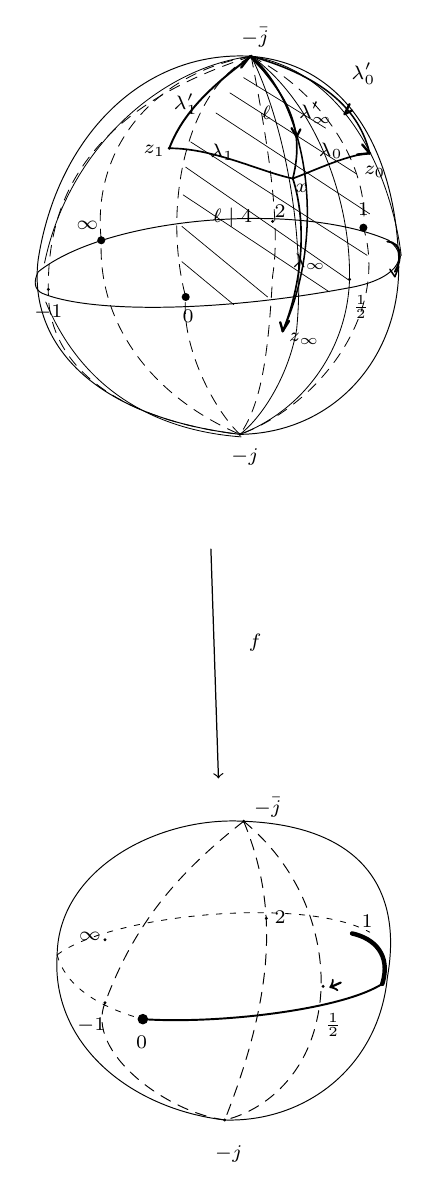
\begin{tikzpicture}[x=.016cm,y=-.016cm,line cap=round,line join=round,font=\scriptsize]
\coordinate (N) at (171,20);
\coordinate (S) at (162,320);
\coordinate (X) at (204,117);
\coordinate (Zone) at (106,93);
\coordinate (Zzero) at (265,97);
\coordinate (Zinf) at (196,238);
\draw[line width=.35pt] (N) .. controls (84,15) and (17,85) .. (2,181)
 .. controls (-6,243) and (39,305) .. (S)
 .. controls (236,319) and (290,260) .. (288,183)
 .. controls (286,105) and (253,27) .. (N);
\draw[line width=.3pt] (N) .. controls (99,29) and (26,93) .. (7,184);
\draw[line width=.3pt] (8,215) .. controls (38,287) and (97,317) .. (163,322);
\draw[line width=.3pt] (N) .. controls (250,33) and (283,121) .. (290,178);
\draw[line width=.35pt] (2,191) .. controls (57,147) and (209,135) .. (280,166)
 .. controls (299,180) and (284,198) .. (247,204)
 .. controls (145,223) and (43,224) .. (5,208)
 .. controls (-1,205) and (-2,199) .. (2,191);
\draw[dash pattern=on 4pt off 3pt,line width=.3pt] (N)
 .. controls (95,33) and (44,92) .. (52,166)
 .. controls (49,232) and (92,290) .. (S);
\draw[dash pattern=on 4pt off 3pt,line width=.3pt] (N)
 .. controls (117,49) and (101,143) .. (119,211)
 .. controls (115,248) and (140,299) .. (S);
\draw[dash pattern=on 4pt off 3pt,line width=.3pt] (N)
 .. controls (183,84) and (195,151) .. (188,194)
 .. controls (185,246) and (181,294) .. (S);
\draw[dash pattern=on 4pt off 3pt,line width=.3pt] (N)
 .. controls (230,50) and (265,110) .. (260,156)
 .. controls (281,225) and (223,298) .. (S);
\draw[dash pattern=on 4pt off 3pt,line width=.3pt] (N)
 .. controls (54,58) and (9,121) .. (10,205)
 .. controls (9,264) and (62,308) .. (S);
\draw[line width=.3pt] (N) .. controls (219,54) and (250,129) .. (249,197)
 .. controls (247,257) and (208,303) .. (S);
\draw[line width=.3pt] (N) .. controls (199,77) and (214,166) .. (207,237)
 .. controls (200,276) and (178,308) .. (S);
\draw[line width=.25pt] (165,37)--(230,77)
 (154,49)--(254,113) (143,65)--(265,145)
 (123,88)--(263,178) (119,108)--(249,198)
 (117,130)--(233,207) (116,155)--(184,211)
 (116,183)--(157,217);
\draw[line width=.7pt] (Zone) .. controls (118,61) and (146,39) .. (N);
\draw[line width=.6pt] (Zone) .. controls (142,93) and (179,112) .. (X);
\draw[line width=.6pt] (X) .. controls (225,109) and (248,98) .. (Zzero);
\draw[line width=.6pt] (X) .. controls (217,158) and (209,207) .. (Zinf);
\draw[line width=.6pt] (N) .. controls (196,49) and (215,73) .. (X);
\draw[line width=.55pt] (N) .. controls (231,37) and (257,64) .. (Zzero);
\draw[line width=.55pt] (N) .. controls (215,58) and (232,159) .. (Zinf);
\draw[line width=.85pt] (163,29)--(170,20)--(181,31);
\draw[line width=.85pt] (259,90)--(265,97)--(255,98);
\draw[line width=.85pt] (201,230)--(196,238)--(194,231);
\draw[line width=.85pt] (249,58)--(245,66)--(251,63);
\draw[line width=.8pt] (203,77)--(207,84)--(210,78);
\draw[line width=.7pt] (279,167) .. controls (291,168) and (291,181) .. (285,191);
\draw[line width=.55pt] (281,189)--(285,195)--(288,187);
\foreach \p in {(171,20),(162,320),(204,117),(106,93),(265,97),(196,238),(10,205),(249,197),(188,151)}
  \fill \p circle[radius=1.3];
\foreach \p in {(52,166),(119,211),(260,156)}
  \fill \p circle[radius=3.2];
\node[inner sep=0pt] at (174,5) {$-\bar j$};
\node[inner sep=0pt] at (166,338) {$-j$};
\node[inner sep=0pt] at (41,154) {$\infty$};
\node[inner sep=0pt] at (194,143) {$2$};
\node[inner sep=0pt] at (260,141) {$1$};
\node[inner sep=0pt] at (10,223) {$-1$};
\node[inner sep=0pt] at (121,226) {$0$};
\node[inner sep=0pt] at (258,219) {$\frac12$};
\node[inner sep=0pt] at (211,125) {$x$};
\node[inner sep=0pt] at (94,95) {$z_1$};
\node[inner sep=0pt] at (269,112) {$z_0$};
\node[inner sep=0pt] at (213,244) {$z_\infty$};
\node[inner sep=0pt] at (148,96) {$\unsure{\lambda_1}$};
\node[inner sep=0pt] at (234,95) {$\lambda_0$};
\node[inner sep=0pt] at (217,183) {$\unsure{\lambda_\infty}$};
\node[inner sep=0pt] at (119,58) {$\unsure{\lambda'_1}$};
\node[inner sep=0pt] at (260,34) {$\lambda'_0$};
\node[inner sep=0pt] at (222,65) {$\unsure{\lambda'_\infty}$};
\node[inner sep=0pt] at (183,65) {$\unsure{\ell}$};
\node[inner sep=0pt] at (156,148) {$\unsure{\ell\mid4}$};
\draw[->,line width=.45pt] (139,411)--(145,593);
\node[inner sep=0pt] at (174,485) {$f$};
\coordinate (NN) at (165,627);
\coordinate (SS) at (150,864);
\draw[line width=.35pt] (NN) .. controls (97,623) and (18,665) .. (17,733)
 .. controls (12,803) and (74,855) .. (SS)
 .. controls (214,866) and (272,822) .. (279,751)
 .. controls (293,672) and (249,630) .. (NN);
\draw[dash pattern=on 4pt off 3pt,line width=.35pt] (NN)
 .. controls (106,673) and (76,715) .. (55,771)
 .. controls (39,810) and (104,858) .. (SS);
\draw[dash pattern=on 4pt off 3pt,line width=.35pt] (NN)
 .. controls (190,688) and (193,755) .. (SS);
\draw[dash pattern=on 4pt off 3pt,line width=.35pt] (NN)
 .. controls (220,672) and (234,739) .. (223,785)
 .. controls (213,831) and (180,857) .. (SS);
\draw[dash pattern=on 2pt off 3pt,line width=.3pt] (17,733)
 .. controls (59,701) and (213,686) .. (265,715);
\draw[dash pattern=on 2pt off 3pt,line width=.3pt] (17,733)
 .. controls (24,759) and (52,775) .. (85,784);
\draw[line width=.7pt] (85,784)
 .. controls (143,788) and (242,777) .. (275,756);
\draw[line width=1.6pt] (251,716)
 .. controls (269,720) and (282,733) .. (275,756);
\draw[->,line width=.8pt] (242,755)--(233,759);
\foreach \p in {(165,627),(150,864),(55,721),(55,771),(183,704),(228,758)}
  \fill \p circle[radius=1.3];
\fill (85,784) circle[radius=4.2];
\node[inner sep=0pt] at (184,616) {$-\bar j$};
\node[inner sep=0pt] at (153,891) {$-j$};
\node[inner sep=0pt] at (43,718) {$\infty$};
\node[inner sep=0pt] at (44,789) {$-1$};
\node[inner sep=0pt] at (84,802) {$0$};
\node[inner sep=0pt] at (236,789) {$\frac12$};
\node[inner sep=0pt] at (263,706) {$1$};
\node[inner sep=0pt] at (194,703) {$2$};
\end{tikzpicture}}

\unsure{donnés} par
\[
\lambda'_i=\bigl(\deleted{\unsure{\tau_i\mid\ell_i}}\dot g_i(\ell^{-1})\bigr)(\lambda_i)\ell.
\]

On a donc
\[
\lambda'_0=
\underbrace{(\dot\sigma_\infty\dot\tau)}_{
\substack{\text{symétrie}\\
\text{p.r. au}\ \deleted{\text{l'équa}}\\
\unsure{\text{plan}}\ (\infty,-\bar j,\frac12,-j)}}
(\ell^{-1})\circ\lambda_0\circ\ell
\]
\inserted{\unsure{tous|est}} homotope au lacet trivial dans
$U_{0,3}$

\[
\lambda'_1=
\underbrace{\dot\sigma_0\dot\tau}_{
\substack{\text{symétrie}\\
\unsure{\text{p.r. à}}\ \text{l'équateur}\\
(0,-\bar j,2,-j)}}
(\ell^{-1})\circ\lambda_1\circ\ell
\]
homotope au lacet trivial dans $U_{0,3}$

\[
\lambda'_\infty=(\underbrace{\tau}(\ell^{-1}))\circ\lambda_\infty\circ\ell
\]
homotope au \deleted{chemin} \inserted{arc de}
grand cercle $(-\bar j,\frac12,-j)$
de $P=\unsure{-\bar j|\bar j}$ vers $\dot\tau P=-j$

\margin{16}
\scanpage{18}
\mspage{297}

En résumé, \unsure{avec} les notations de [C] \deleted{(13)} p.~7 \unsure{ff}, on aura donc
\[
\left\{
\begin{aligned}
\tau'_0&=\widetilde{\sigma}_\infty &&(\text{sur }\dot{\sigma}_\infty\dot{\tau})\\
\tau'_1&=\widetilde{\sigma}_0 &&(\text{sur }\dot{\sigma}_0\dot{\tau})\\
\tau'_\infty&=\tau_\infty &&(\text{sur }\dot{\tau})
\end{aligned}
\right.
\tag{22}
\]
\margin{NB $\tau_\infty=\sigma_\infty\widetilde{\sigma}_\infty=\widetilde{\sigma}_\infty\sigma_\infty$}

Il faut vérifier les relations essentielles
\[
\tau_0^{\prime\,2}=\tau_1^{\prime\,2}=\tau_\infty^{\prime\,2}
=\bigl(\underbrace{\tau'_0\tau'_\infty}_{\sigma_\infty}\bigr)^2
=\bigl(\underbrace{\tau'_1\tau'_0}_{\rho^{-1}}\bigr)^3=1
\tag{23}
\]
les quatre premières sont claires, la dernière s'écrit
\[
(\widetilde{\sigma}_0\widetilde{\sigma}_\infty)^3=1
\]
or on a
\[
\widetilde{\sigma}_0\widetilde{\sigma}_\infty=\rho^{-1}
\qquad (\inserted{[C],}\ \text{formule 13,})
\]
d'où ce qu'on veut.

Calculons (\unsure{conformément} à (18)) $\tau'_\infty\tau'_1$, $\tau'_0\tau'_\infty$, $\underbrace{\tau'_1\tau'_0}_{\rho^{-1}}$ --- qui \unsure{devront correspondre} à $\ell'_0,\ell'_1,\ell'_\infty$ ---
\[
\begin{aligned}
\ell'_0&=\tau'_\infty\tau'_1=\tau_\infty\widetilde{\sigma}_0
=\sigma_\infty\underbrace{\widetilde{\sigma}_\infty\widetilde{\sigma}_0}_{\rho}
=\sigma_\infty\rho\\
\ell'_1&=\tau'_0\tau'_\infty=\sigma_\infty\\
\ell'_\infty&=\tau'_1\tau'_0=\rho^{-1}
\end{aligned}
\]
i.e.
\[
\ell'_0=\sigma_\infty\rho,\quad \ell'_1=\sigma_\infty,\quad \ell'_\infty=\rho^{-1}
\tag{24}
\]
avec les relations caractéristiques
\[
\ell'_\infty\ell'_1\ell'_0=1,\qquad \ell_{\unsure{1|\infty}}^{\prime\,2}=1,\qquad \ell_\infty^{\prime\,3}=1
\tag{25}
\]
Tout est OK !

\margin{On exprime les éléments remarquables $\rho,\sigma_0,\sigma_1,\sigma_\infty,\ell_0,\ell_1,\ell_\infty,\tau_0,\tau_1,\tau_\infty$ de $\Pi_1(U_{0,3}^{\mathrm{an}};\mathfrak S_3\times\mathbb Z/2)$ en fonction des $\tau'_0,\tau'_1,\tau'_\infty$ ainsi :
\[
\begin{aligned}
\rho&=\tau'_0\tau'_1\\
\tau_\infty&=\tau'_\infty,\quad
\tau_0=\rho\tau_\infty\rho^{-1}=\tau'_0\tau'_1\tau'_\infty\tau'_1\tau'_0,\\
\tau_1&=\rho^{-1}\tau_\infty\rho=\ldots=\tau'_1\tau'_\infty\tau'_1
\end{aligned}
\]
\inserted{\unsure{$=\tau'_\infty\tau'_0$}}
\[
\begin{aligned}
\sigma_\infty&=\tau'_0\tau'_\infty,\quad
\sigma_0=\rho\sigma_\infty\rho^{-1}=\tau'_0\tau'_1\tau'_0\tau'_\infty\unsure{\tau'_1\tau'_0},\\
\sigma_1&=\rho^{-1}\sigma_\infty\rho=\tau'_1\tau'_\infty\tau'_0\tau'_1\\
\ell_0&=\tau_\infty\tau_1=\tau'_\infty\tau'_1\tau'_\infty\tau'_1=(\tau'_\infty\tau'_1)^2\\
\ell_1&=\tau_0\tau_\infty=\tau'_0\tau'_1\tau'_\infty\tau'_1\tau'_0\unsure{\tau'_\infty}\\
\ell_\infty&=\tau_1\tau_0=(\underbrace{\tau'_1\tau'_\infty\tau'_1}\tau'_0)^2
\end{aligned}
\]
\[
\begin{aligned}
\varepsilon_0&=\ell'_0=\deleted{\unsure{\tau'_1\tau'_\infty}}\unsure{\tau'_\infty\tau'_1}\\
\varepsilon_1&=\unsure{\tau'_0\tau'_1\tau'_\infty\tau'_0}\\
\varepsilon_\infty&=\tau'_1\tau'_\infty\tau'_1\unsure{\tau'_0}
\end{aligned}
\]
}
\margin{17}
\scanpage{19}

Je voudrais encore expliciter la \unsure{relation} de
$\widetilde{\Pi}'_{0,3}$ \inserted{gr. \unsure{carto-graphique} non orienté}
$\simeq\mathfrak S_{0,3}$ \inserted{$=\mathrm{Aut}_{\unsure{\mathrm{loc}|\mathrm{ext}}}(\Pi_{0,3})$}
avec $\mathrm{GP}(1,\mathbb Z)\simeq\mathrm{Gl}(2,\mathbb Z)'\overset{\mathrm{def}}{=}\mathrm{Gl}(2,\mathbb Z)/\{\pm1\}$.
Rappelons d'abord l'opération de
\[
\mathrm{GP}(1,\mathbb R)\simeq\mathrm{Gl}(2,\mathbb R)/\mathbb R^*
\simeq\mathrm{Gl}(2,\mathbb R)^{\pm1}/\{\pm1\}\quad\deleted{\unsure{\mathrm{GP}(|\text{agit}}}
\tag{26}
\]
sur le demi-plan de Poincaré $D$
\[
D=\{z\in\mathbb C\mid\Im(z)>0\}=\{x+iy\mid x\in\mathbb R,y\in\mathbb R^{*+}\}.
\tag{27}
\]
On fait opérer la matrice $u=\begin{pmatrix}a&b\\c&d\end{pmatrix}$ par
\[
f_u(z)=\left\{\begin{array}{ll}
\dfrac{az+b}{cz+d}&\text{si }\det u>0\\[4pt]
\dfrac{a\bar z+b}{c\bar z+d}&\text{si }\det u<0
\end{array}\right.
\tag{28}
\]
De cette façon, $\mathrm{GP}(1,\mathbb R)$ est isomorphe au groupe des automorphismes \uline{conformes} de $D$.

\margin{\uline{NB} $\mathrm{GP}(1,\mathbb R)$ a deux \unsure{comp. connexes}. \unsure{Sa comp. neutre} \inserted{$\mathrm{GP}(1,\mathbb R)^+$} est l'image de $\mathrm{Sl}(2,\mathbb R)$ (\unsure{ou de|de} $\mathrm{Gl}(2,\mathbb R)^+$) et s'identifie à $\mathrm{Sl}(2,\mathbb R)/\pm1$.}

D'ailleurs, la donnée d'une courbe elliptique \inserted{$E$} sur $\mathbb C$ équivaut à celle d'un espace $V$ de dim 1 sur $\mathbb C$, et d'un ``réseau'' $\pi\subset V$ (sous-groupe discret de rg 2).
\margin{équivalence de catégories \illegible{1}.}
L'orientation canonique de $V$ correspond à un générateur \unsure{$\eta|\gamma$} de $\bigwedge^2_{\mathbb Z}\pi$ --- ainsi $\pi$ est ``orienté''. Le choix d'une rigidification
\margin{18}
\scanpage{20}
\mspage{298}

de Jacobi unimodulaire de $\pi$, équivaut à celui d'une base $(e_1,e_2)$ de $\pi$ \inserted{(comme $\mathbb Z$-module)} telle que $e_1\wedge e_2=\unsure{\eta|\gamma}$. L'élément $e_1$ \inserted{(comme base de $V$ sur $\mathbb C$)} permet d'ailleurs d'identifier $V$ à $\mathbb C$, $e_1$ devenant 1. Ainsi la donnée de $E$ avec sa rigidification de Jacobi unimodulaire, équivaut à celle d'un élément $e_2=\tau$ de $\unsure{\mathbb C|E}$, tel que

\uline{1\textsuperscript{o}}) $(1,\tau)$ \unsure{engendrent|engendre} un sous-groupe discret de rg 1, i.e. $\tau\notin\mathbb R$ i.e. $\Im\tau\ne0$

2\textsuperscript{o}) l'orientation dudit sous-groupe définie par la base $(1,\tau)$ est ``directe'', i.e. $\Im\tau>0$, i.e. $\tau\in D$.

Quand on regarde l'opération de $\mathrm{Sl}(2,\mathbb Z)$ sur \inserted{l'ens} des classes d'isomorphie des courbes ell. rigidifiées, \unsure{ens.} \unsure{identifié} à $D$, on trouve que $\begin{pmatrix}a,b\\c,d\end{pmatrix}$ opère par $\tau\longmapsto\dfrac{a\tau+b}{c\tau+d}$, i.e. c'est l'opération naturelle de $\mathrm{Sl}(2,\mathbb Z)$ sur $D$, à travers $\mathrm{Sl}(2,\mathbb Z)'\simeq\mathrm{GP}(1,\mathbb Z)^+$.

Ce groupe opère proprement, Il a exactement deux trajectoires critiques, qui corres-
\margin{19}
% ===== LM_P061: second pass, checked against the scans =====
\scanpage{21}

pondent respectivement aux $\tau$ qui \unsure{avec} $1$ \unsure{engendrent} \unsure{l'un} réseau des entiers alg. de $\mathbb{Q}(i)$ (soit $\mathbb{Z}+i\mathbb{Z}$), et le réseau des entiers de $\mathbb{Q}(j)$, formé des nbs de la forme $aj+b\bar{j}$ ($j=\dfrac{-1+i\sqrt{3}}{2}=\exp\dfrac{2i\pi}{3}$); la ramification \unsure{correspondante} est $2$ et $3$.

On a un isom. canonique (analytique) \inserted{\unsure{entre}}
\[
\tag{29}
D/\mathrm{GP}(1,\mathbb{Z})^{+}\simeq\mathbb{P}^{1\,\mathrm{an}}\setminus\{0\}=Y,
\]
\unsure{caractérisé} par la condition que l'orbite critique de ramification $3$ \unsure{corresponde} au point $\infty$, et celle de ramification $2$ au point $1$. On trouve ainsi un isom
(posant $\mathcal{G}=\mathrm{GP}(1,\mathbb{Z})$, $G=\mathrm{GP}(1,\mathbb{Z})^{+}=\mathrm{Sl}(2,\mathbb{Z})'$)

(30)
\diagram{
\begin{tikzcd}[ampersand replacement=\&,column sep=large]
\pi_1(D,\mathcal{G},x)
  \arrow[r,"\sim"] \arrow[d,equal]
\& \pi_1^{\unsure{\pm|*}}(Y,\underline{d};y) \\
\mathcal{G} \&
\end{tikzcd}
}
\margin{$(x\in D\setminus\unsure{D^{!}|D'})$}

que je voudrais expliciter, en identifiant \deleted{les} $\tau'_0,\tau'_1,\tau'_\infty$ comme \unsure{éléments} de $\mathrm{Gl}^{\unsure{\pm'|\pm}}(2,\mathbb{Z})'$.

\margin{\unsure{0}}
\margin{20}
\scanpage{22}
\mspage{299}

\uline{39} \deleted{\unsure{Propriétés}}\inserted{Les} conditions de congruence
pour l'opération extérieure de $\Gamma_{\mathbb Q}$ sur $\widehat{\Pi}_{0,3}$.

Considérons le diagramme

\[
\tag{1}
\diagram{\begin{tikzcd}[ampersand replacement=\&,column sep=large,row sep=small]
1 \arrow[r] \& \widehat{\mathcal T}_{1,1}^{+} \arrow[r] \arrow[d,phantom,"\simeq" description,sloped] \& N_{1,1} \arrow[r] \arrow[dd] \& \Gamma_{\mathbb Q} \arrow[r] \arrow[dd,"\chi"] \& 1 \\
\& \mathrm{Sl}(2,\mathbb Z)^{\wedge} \arrow[d] \& \& \& \\
1 \arrow[r] \& \mathrm{Sl}(2,\widehat{\mathbb Z}) \arrow[r] \& \mathrm{Gl}(2,\widehat{\mathbb Z}) \arrow[r,"\det"] \& \widehat{\mathbb Z}^{*} \arrow[r] \& 1
\end{tikzcd}}
\]

Il montre que l'opération extérieure de
$\Gamma_{\mathbb Q}$ sur $\widehat{\mathcal T}_{1,1}^{+}$
\inserted{$\simeq \mathrm{Sl}(2,\mathbb Z)^{\wedge}$}
passe \unsure{en|au} quotient en une
action extérieure sur $\mathrm{Sl}(2,\widehat{\mathbb Z})$, et cette
action extérieure, de plus, peut s'expliciter
entièrement à l'aide du caractère
cyclotomique
\[
\tag{2}
\chi : \Gamma_{\mathbb Q}\longrightarrow \widehat{\mathbb Z}^{*}.
\]

Pour préciser ce dernier point, notons
que la deuxième ligne de (1) donne
un homomorphisme
\[
\tag{3}
\widehat{\mathbb Z}^{*}\longrightarrow
\mathrm{Autext}(\mathrm{Sl}(2,\widehat{\mathbb Z})),
\]
et l'hom canonique
\[
\tag{4}
\Gamma_{\mathbb Q}\longrightarrow
\deleted{\unsure{\mathrm{Sl}(2,}}
\mathrm{Autext}(\mathrm{Sl}(2,\widehat{\mathbb Z}))
\]
\margin{21}
\scanpage{23}

n'est autre que le composé de (2) et (3).
Par ailleurs, l'hom. (4) se factorise
en
\[
\tag{5}
\widehat{\mathbb Z}^{*}/\widehat{\mathbb Z}^{*2}
\longrightarrow \mathrm{Autext}(\mathrm{Sl}(2,\widehat{\mathbb Z}))
\]

(\unsure{provient} du fait que les \unsure{éléments|élts} de
$\mathrm{Gl}(2,\widehat{\mathbb Z})$ qui sont dans le centre
$\widehat{\mathbb Z}^{*}$ opèrent trivialement
\deleted{\unsure{du point}}\inserted{sur} $\mathrm{Sl}(2,\widehat{\mathbb Z})$,
et que le composé
\[
\widehat{\mathbb Z}^{*}\xrightarrow{\text{(centre)}}
\mathrm{Gl}(2,\widehat{\mathbb Z})\xrightarrow{\det}
\unsure{\widehat{\mathbb Z}|\mathbb Z}^{\unsure{*|2}}
\]
n'est autre que $\lambda\longmapsto\lambda^{\unsure{2}}$). Plus
précisément, on voit que pour que l'
\unsure{autom} de $\mathrm{Sl}(2,\widehat{\mathbb Z})$ induit par un
$u\in\mathrm{Gl}(\unsure{1|2},\widehat{\mathbb Z})$ soit intérieur,
\unsure{i.d.|i.e.} de la forme
$\mathrm{int}\,\unsure{(u_0)|u_0}$ avec $u_0\in\mathrm{Sl}(2,\widehat{\mathbb Z})$, il f. et s.
qu'il existe $u_0\in\mathrm{Sl}(2,\widehat{\mathbb Z})$ tel que
$u^{\unsure{\deleted{0}|\circ}}u_0^{-1}$ commute à $\mathrm{Sl}(2,\widehat{\mathbb Z})$, et cela signifie
que c'est un scalaire -- i.e.
$u\in\mathrm{Sl}(2,\widehat{\mathbb Z})\cdot\widehat{\mathbb Z}^{*}$\unsure{,|.}
En d'autres termes
l'hom (5) est \uline{injectif}, et en conséquence,
\margin{22}
\scanpage{24}
\mspage{300}

le noyau de (4) n'est autre que le
noyau du composé
\[
\tag{6}
\Gamma_{\mathbb Q}\xrightarrow{\chi}\widehat{\mathbb Z}^{*}
\longrightarrow\widehat{\mathbb Z}^{*}/\widehat{\mathbb Z}^{*2}
\]
i.e. (par la théorie du corps de classes pour
$\mathbb Q$) l'opération \inserted{ext} de $\Gamma_{\mathbb Q}$ sur
$\mathrm{Sl}(\unsure{1|2},\widehat{\mathbb Z})$ se
factorise par une opération \inserted{ext} de
$(\Gamma_{\mathbb Q\,\mathrm{ab}})_2$ -- le
\unsure{quotient} ``multiquadratique'' de $\Gamma_{\mathbb Q}$ -- et cette
dernière est fidèle.

\margin{\uline{NB} L'op. ext. de $\Gamma_{\mathbb Q}$ sur
$\mathrm{Sl}(2,\mathbb Z/\unsure{n|m}\mathbb Z)$ se fait par
l'\unsure{intermédiaire} de
$\unsure{((\mathbb Z/\unsure{n|m}\mathbb Z)^{*})_2|(\mathbb Z/\unsure{n|m}\mathbb Z)_2^{*}}$}

Ainsi, si on identifie $\Gamma_{\mathbb Q}$ \deleted{\unsure{par (4)}}
à un sous-groupe de $\mathrm{Autext}\,\mathrm{Sl}(2,\widehat{\mathbb Z})^{\wedge}$,
ce sous-groupe \inserted{$\unsure{\Gamma}$} est astreint à des
conditions assez fortes : \deleted{\illegible{1}} invarier
le sous-groupe distingué noyau de
\[
\tag{7}
\mathrm{Sl}(2,\mathbb Z)^{\wedge}\longrightarrow
\mathrm{Sl}(2,\widehat{\mathbb Z})
\]
et induire sur $\mathrm{Sl}(2,\widehat{\mathbb Z})$
\deleted{\unsure{l'}}\inserted{une} opération extérieure
provenant d'un hom $\Gamma\longrightarrow
\widehat{\mathbb Z}^{*}/\widehat{\mathbb Z}^{*2}$.
On peut d'ailleurs préciser cet hom.
ainsi. Considérons dans $\mathrm{Sl}(2,\widehat{\mathbb Z})$ le
``sous-groupe-lacets'' provenant du point à
\margin{23}
\scanpage{25}

l'infini de $M_{1,1\,\mathbb Q}$, il correspond
à une classe d'hom. ext.
\[
(8)\qquad
T=T_{\infty}(\overline{\mathbb Q}_{0})
\longrightarrow
\mathrm{Sl}(2,\overset{\unsure{\deleted{\wedge}|\wedge}}{\mathbb Z})^{\wedge}
\]
dont l'image \inserted{dans $\mathrm{Sl}(2,\widehat{\mathbb Z})$}
sauf erreur, est (à conj. près) un sous-groupe ``unipotent''
\[
(9)\qquad
\left(\begin{array}{cc}1&0\\ n&1\end{array}\right),
\qquad n\in\widehat{\mathbb Z}.
\]

Cet hom extérieur est respecté par l'opération de $\Gamma$, d'où une opération
bien déterminée de $\Gamma$ sur \deleted{$\unsure{\mathrm{Sl}(2,}$} $T$
i.e. un hom
\deleted{$\Gamma\longrightarrow\operatorname{Aut}(T)\simeq\widehat{\mathbb Z}^{*}$}
\deleted{(qui \illegible{1} sera, justement $\unsure{\chi}$, le}
\[
(10)\qquad
\Gamma\xrightarrow{\chi}\operatorname{Aut}(T)
\simeq\widehat{\mathbb Z}^{*},
\]
qui sera justement le caractère cyclotomique.
De façon plus précise, pour \unsure{un|Un} automorphisme extérieur \inserted{$u$} de
$\mathrm{Sl}(2,\mathbb Z)^{\wedge}$ (ou seulement de $\mathrm{Sl}(2,\widehat{\mathbb Z})$)
qui invarie \unsure{la|l'} \deleted{\unsure{im.}} \unsure{classe} de \unsure{conjugais.|conjugais}
de l'image de (8) [ou \unsure{seulement|seulmt} du composé
$T\unsure{\longrightarrow}\mathrm{Sl}(2,\widehat{\mathbb Z})$],
\inserted{on vérifie qu'}il existe un
$\chi(u)\in\operatorname{Aut}(T)\simeq\widehat{\mathbb Z}^{*}$ unique,
tel que l'on ait commutativité dans
\margin{faire la vérification}
\margin{24}
\scanpage{26}
\mspage{301}

\[
(11)\qquad
\diagram{\begin{tikzcd}[ampersand replacement=\&]
T \arrow[r, "\unsure{\kappa|k}"] \arrow[d, "\chi(u)"]
 \& \mathrm{Sl}(2,\mathbb Z)^{\wedge} \arrow[d, "u"] \\
T \arrow[r]
 \& \mathrm{Sl}(2,\mathbb Z)^{\wedge}
\end{tikzcd}}
\]
--- ou \unsure{même}, seulement dans
\[
(12)\qquad
\diagram{\begin{tikzcd}[ampersand replacement=\&]
T \arrow[r, "\unsure{\kappa|k}"] \arrow[d, "\chi(u)"]
 \& \mathrm{Sl}(2,\widehat{\mathbb Z}) \arrow[d, "\dot u"] \\
T \arrow[r]
 \& \mathrm{Sl}(2,\widehat{\mathbb Z})
\end{tikzcd}}
\quad ---
\]
d'où un caractère \inserted{$\chi$} (10) sur le
groupe de tous les autom. \inserted{ext.} $u$ de
$\mathrm{Sl}(2,\widehat{\mathbb Z})$ qui ont la propriété \unsure{envisagée}.

Ceci dit, $\Gamma$ est contenu dans ce sous-groupe \inserted{$\unsure{\Gamma}$},
et de plus dans le sous-groupe des autom. ext. qui \uline{de plus}
préservent le noyau de (7), et qui opèrent \inserted{(ext.!)} dans le quotient
$\mathrm{Sl}(2,\widehat{\mathbb Z})$ suivant le composé
\[
\Gamma\unsure{:}\xrightarrow{\chi}\widehat{\mathbb Z}^{*}
\longrightarrow\widehat{\mathbb Z}^{*}/\widehat{\mathbb Z}^{*2}
\hookrightarrow\operatorname{Autext}_{\mathrm{lac}!}
(\mathrm{Sl}(2,\widehat{\mathbb Z})).
\]

\deleted{L'on} D'ailleurs notons que le centre $\{\pm1\}$
de $\mathrm{Sl}(2,\mathbb Z)^{\wedge}$ n'étant pas trivial, l'op. ext.
\margin{25}
\scanpage{27}

de $\Gamma_{\mathbb Q}$ sur
$\widehat{\mathcal T}_{1,1}^{+}$
ne permet pas à priori de reconstituer (à iso unique près)
l'ext. $N_{1,1}$ de $\Gamma_{\mathbb Q}$ par
$\widehat{\mathcal T}_{1,1}^{+}$
de (1). Elle donne seulement l'extension \deleted{\illegible{1}}
$N'_{1,1}$ de $\Gamma_{\mathbb Q}$ par
\[
\widehat{\mathcal T}_{1,1}^{+\prime}
\simeq\mathrm{Sl}(2,\mathbb Z)^{\wedge}/\{\pm1\}
\inserted{\overset{\unsure{\mathrm{dfn}|\mathrm{déf}}}{=}
\mathrm{Sl}(2,\widehat{\mathbb Z})'}
\]
(par image inverse de l'extension

\diagram{\begin{tikzcd}[ampersand replacement=\&,column sep=1.1em,row sep=1.0em]
{(13)\quad 1}\arrow[r] \&
\mathrm{Sl}(2,\widehat{\mathbb Z})'\arrow[r] \&
\operatorname{Aut}\deleted{\unsure{\mathrm{ext}}}_{\mathrm{lac}}\bigl(\mathrm{Sl}(2,\unsure{\mathbb Z})^{\wedge}\bigr)\arrow[r] \&
\operatorname{Autext}_{\mathrm{lac}}\,\unsure{\mathrm{Sl}(2,\mathbb Z)^{\wedge}}\arrow[d]\\
\&\&\&1
\end{tikzcd}}

Cette extension \inserted{$N'_{1,1}$} a été aussi interprétée
comme l'extension $M_{0,3}\simeq N'_{0,4}$ de
$\Gamma_{\mathbb Q}$ par
$\widehat{\mathfrak S}_{0,3}
\simeq\widehat{\mathcal T}_{0,4}'$
(groupe qui est lui-$\overline{\mathrm m}$ ext de
$\mathfrak S_3\simeq\mathrm{Sl}(2,\mathbb Z/2\mathbb Z)$
par $\widehat{\Pi}_{0,3}$).
Nous savons déjà que l'opération \inserted{ext} de $\Gamma_{\mathbb Q}$
sur le noyau $\widehat{\Pi}_{0,3}$ de
$\mathrm{Sl}(2,\overset{\unsure{\deleted{\wedge}|\wedge}}{\mathbb Z})^{\wedge\prime}
\longrightarrow\mathrm{Sl}(2,\unsure{\mathbb Z/2|\mathbb Z_{2}})$
est fidèle, et commute à l'op. ext. de
$\mathfrak S_3\simeq\mathrm{Sl}(2,\mathbb Z/2\mathbb Z)
\simeq\mathrm{Sl}(2,\mathbb Z)^{\wedge\prime}/\widehat{\Pi}_{0,3}$.
Mais cette commutation peut mainte-
\margin{26}
\scanpage{28}
\mspage{302}
nant s'interpréter comme conséquence du fait que l'opération ext. de $\Gamma_{\mathbb Q}$ sur $\mathfrak S_3\simeq \mathrm{Sl}(2,\mathbb Z/2\mathbb Z)$ est triviale, elle-$\overline{\mathrm m}$ \inserted{(dans l'optique présente)} conséquence du fait qu'elle \unsure{se fait} par l'intermédiaire d'une op. (fidèle) de $(\mathbb Z/n\mathbb Z)^*_{\unsure{/2|2}}$, or pour $n=2$ $(\mathbb Z/n\mathbb Z)^*_2=1$ (relation qui est par contre fausse pour \deleted{\unsure{les}} \inserted{\unsure{autres|d'autres}} \unsure{valeurs}, $n\neq\deleted{\unsure{2,}}1,2$ i.e. $n\geq3$). Cette relation de commutation, de nature assez triviale, apparaît donc à présent comme un cas très particulier des relations congruentielles nettement plus subtiles. On peut \inserted{essayer de} les exprimer \deleted{\unsure{de}} \deleted{façon} directement en termes de l'opération ext. de $\Gamma_{\mathbb Q}$ sur $\widehat\Pi_{0,3}$, en introduisant les noyaux des \unsure{hom.} $\widehat{\mathcal T}_{1,1}^{\unsure{+\prime|+/n}}\longrightarrow \mathrm{Sl}(2,2m)$, qui sont des sous-groupes \deleted{$\Pi(2m)$} ouverts :
\[
(14)\qquad \Pi(2m)\subset\widehat\Pi_{0,3}
\]
distingués et invariants par $\mathfrak S_3$, noyaux
\margin{27}
\scanpage{29}
d'homomorphismes
\[
(15)\qquad \varphi_{2m}:\widehat\Pi_{0,3}\longrightarrow\mathrm{Sl}(2,\mathbb Z/2m)'
\]
qu'il \unsure{en|ne} doit pas être bien difficile d'expliciter, \deleted{\unsure{en termes}} \inserted{par ``réduction mod $2m$''} d'un \unsure{hom.}
\[
(16)\qquad \varphi_{\infty}:\widehat\Pi_{0,3}\longrightarrow\mathrm{Sl}(2,\widehat{\mathbb Z})'
\]
dont il a été question déjà précédemment -- \unsure{hom.} dont l'image est le sous-groupe noyau de $\mathrm{Sl}(2,\widehat{\mathbb Z})'\longrightarrow\mathrm{Sl}(2,\mathbb Z/2\mathbb Z)$, i.e. on a une suite exacte
\[
(17)\qquad \deleted{1\longrightarrow\Pi(\unsure{2m})\longrightarrow}\inserted{1\longrightarrow\Pi(\infty)\longrightarrow}\widehat\Pi_{0,3}\longrightarrow\mathrm{Sl}(2,\widehat{\mathbb Z})'\longrightarrow\mathrm{Sl}(2,\mathbb Z/2\mathbb Z)\longrightarrow1
\]
\[
(18)\qquad 1\longrightarrow\Pi(2m)\longrightarrow\widehat\Pi_{0,3}\longrightarrow\mathrm{Sl}(2,\mathbb Z/2m\mathbb Z)'\longrightarrow\mathrm{Sl}(2,\mathbb Z/2\mathbb Z)\longrightarrow1.
\]
Ceci posé, \unsure{ces|les} suites exactes permettent de façon naturelle de définir une opération ext. de $\widehat{\mathbb Z}^{*}/\widehat{\mathbb Z}^{*2}$ sur $\widehat\Pi_{0,3}/\Pi(\infty)$, ou encore des $(\mathbb Z/2m\mathbb Z)^*_2$ sur les $\widehat\Pi_{0,3}/\Pi(2m)$, et la ``condition de \unsure{congruence|congruences}'' s'exprime en disant que le caractère cyclotomique $\chi$ de $\Gamma_{\mathbb Q}$ (\inserted{qu'on peut considérer comme} déduit de l'opération ext. de
\margin{28}
\scanpage{30}
\mspage{303}
$\Gamma_{\mathbb Q}$ sur \unsure{le|les} \unsure{groupe|groupes} à lacets $\widehat\Pi_{0,3}$), qui donne \unsure{un|en} composé
\[
(19)\qquad \Gamma_{\mathbb Q}\xrightarrow{\chi}\widehat{\mathbb Z}^{*}\xrightarrow{\mathrm{can.}}\widehat{\mathbb Z}^{*}/\widehat{\mathbb Z}^{*2},
\]
\unsure{de|donc} une op. ext. de $\Gamma_{\mathbb Q}$ sur $\widehat\Pi_{0,3}/\Pi(\infty)$, est \uline{compatible} avec l'op. ext. de $\Gamma_{\mathbb Q}$ sur $\widehat\Pi_{0,3}$ lui-$\overline{\mathrm m}$.

Pour chaque entier $m$, cette condition s'explicite par le fait que $\Pi(2m)$ est invariant par l'op. ext. de $\Gamma_{\mathbb Q}$, et que l'opération ext. induite \unsure{de|sur} $\widehat\Pi_{0,3}/\Pi(2m)$ est celle déduite du caractère composé de (19) avec
\[
\widehat{\mathbb Z}^{*}/\widehat{\mathbb Z}^{*2}\longrightarrow(\mathbb Z/\unsure{2m|m}\mathbb Z)^*_2:
\]
\[
(20)\qquad \Gamma_{\mathbb Q}\longrightarrow(\mathbb Z/m\mathbb Z)^*_2.
\]
On devrait regarder si cette formulation est vraiment \uline{équivalente} à celle des conditions de \unsure{congruences|congruence} dans $\widehat{\mathcal T}_{1,1}^{+\prime}$ \unsure{tout} entier, \deleted{(\unsure{quitte à y} \illegible{1}} \inserted{et non seulement une} conséquence; \unsure{exercice|exercices} ! Par contre, \unsure{le|la}
\margin{29}
% ===== LM_P062: second pass, checked against the scans =====
\scanpage{31}

question de savoir si les conditions constituent bel et bien une restriction, effective, sur un autom. ext. du groupe à lacets $\widehat{\Pi}_{0,3}$, commutant à l'action de $\mathfrak{S}_3$, \unsure{risque} fort d'être hors de portée, faute de savoir construire effectivement de tels autom. extérieurs \inserted{(\unsure{on|ou} \illegible{1} des \unsure{élémts} \unsure{non triviaux} de $\unsure{\widehat{\widehat{\mathcal{T}}}|\widehat{\mathcal{T}}}_{0,3}^{!\unsure{*}}$)} d'une autre façon que justement par voie arithmétique, à l'aide de l'opération de $\Gamma_{\mathbb{Q}}$ sur $\widehat{\Pi}_{0,3}$ ! (Il faudrait quand \unsure{même} refaire à l'occasion un effort en ce sens \ldots)

Je me pose aussi la question \unsure{dans|de} quelle mesure on peut reconstituer, en termes de la théorie des groupes profinis à lacets et des \deleted{\unsure{leurs}} autom. ext. de $\widehat{\Pi}_{0,3}$, ou de \deleted{\illegible{1}}\inserted{$\widehat{\mathfrak{S}}_{0,3}^{+}$} $\simeq \widehat{\mathcal{T}}_{1,1}^{+\prime}$, \deleted{l'hom.}

\margin{30}
\scanpage{32}
\mspage{304}

a) l'extension plus fine $N_{1,1}$ de $\Gamma_{\mathbb{Q}}$ par $\widehat{\mathcal{T}}_{1,1}^{+}$, qui est donc une ext. de $N'_{1,1}$ (\unsure{censé} être connu) par le groupe $\{\pm1\}$

b) l'hom
\[
\begin{array}{|c|}
\hline
N_{1,1}\longrightarrow \mathrm{Gl}(2,\widehat{\mathbb{Z}})
\end{array}
\tag{21}
\]
de (1), et à défaut, l'hom
\deleted{$N'_{1,1}\simeq\widehat{\mathfrak{S}}_{0,3}^{+}$}
\[
N'_{1,1}\simeq
\deleted{\unsure{\mathfrak{S}}}\inserted{M}_{0,3}^{\deleted{\unsure{+}}}
\longrightarrow
\mathrm{Gl}(2,\widehat{\mathbb{Z}})/\{\pm1\}.
\tag{22}
\]

Je \unsure{commencerai|commence} par la question b).

Si on dispose de l'extension $N_{1,1}$ de $\Gamma_{\mathbb{Q}}$ par $\widehat{\mathcal{T}}_{1,1}^{+}\inserted{\simeq\mathrm{Sl}(2,\mathbb{Z})^{\wedge}}$, on a un hom
\[
N_{1,1}\longrightarrow
\mathrm{Aut}_{\mathrm{lac}}
\left(\underbrace{\widehat{\mathcal{T}}_{1,1}^{+}}_{\mathrm{Sl}(2,\mathbb{Z})^{\wedge}}\right)
\tag{23}
\]
qui passe au quotient en un hom
\[
N_{1,1}\longrightarrow
\mathrm{Aut}_{\mathrm{lac}}\left(\mathrm{Sl}(2,\widehat{\mathbb{Z}})\right)
\tag{24}
\]
or on a un hom évident
\[
\deleted{\illegible{1}}\quad
\mathrm{Gl}(2,\widehat{\mathbb{Z}})
\longrightarrow
\mathrm{Aut}_{\mathrm{lac}}\left(\mathrm{Sl}(2,\widehat{\mathbb{Z}})\right)
\]
qui se factorise en
\[
\mathrm{Gl}(2,\widehat{\mathbb{Z}})
\longrightarrow
\mathrm{Gl}(2,\widehat{\mathbb{Z}})/\widehat{\mathbb{Z}}^{*}
\simeq \mathrm{GP}(1,\widehat{\mathbb{Z}})
\hookrightarrow
\mathrm{Aut}_{\mathrm{lac}}\left(\mathrm{Sl}(2,\widehat{\mathbb{Z}})\right)
\tag{25}
\]
et il se trouve que (24) se factorise en
\[
N_{1,1}\longrightarrow
\underset{\simeq\,\mathrm{Gl}(\unsure{2|1},\widehat{\mathbb{Z}})/\widehat{\mathbb{Z}}^{*}}
{\mathrm{GP}(1,\widehat{\mathbb{Z}})}
\hookrightarrow
\mathrm{Aut}_{\mathrm{lac}}\left(\mathrm{Sl}(2,\widehat{\mathbb{Z}})\right)
\tag{26}
\]

\margin{31}
\scanpage{33}

ce qui permet donc de reconstituer, à partir de l'extension $N_{1,1}$, un hom
\[
N_{1,1}\xrightarrow{\varphi}
\mathrm{GP}(1,\widehat{\mathbb{Z}})
\simeq
\mathrm{Gl}(2,\widehat{\mathbb{Z}})/\widehat{\mathbb{Z}}^{*},
\tag{27}
\]
un peu plus faible que l'hom (21) qu'on cherche à construire. Mais notons que l'hom
\[
\diagram{
\begin{tikzcd}[ampersand replacement=\&, column sep=small,row sep=small]
\mathrm{Gl}(2,\widehat{\mathbb{Z}})
\arrow[r,"{u\mapsto(\dot{u},\det(u))}"]
\&
\mathrm{GP}(1,\widehat{\mathbb{Z}})\arrow[d]
\&
{}\times\widehat{\mathbb{Z}}^{*}
\\
\&
\widehat{\mathbb{Z}}^{*}/\widehat{\mathbb{Z}}^{*2}
\&
\end{tikzcd}
}
\tag{28}
\]
a comme \uline{noyau} l'ens des $\lambda\in\widehat{\mathbb{Z}}^{*}$ tels que $\lambda^2=1$ -- i.e. le groupe
\[
{}_{2}\widehat{\mathbb{Z}}^{*}
\simeq (\mathbb{Z}/2\mathbb{Z})^{P}
\tag{29}
\]
\margin{$P\unsure{=|:}$ ens des nbs premiers}

Ainsi, on trouve que l'hom
\[
\deleted{\unsure{\Gamma_{\mathbb{Q}}}}\inserted{N_{1,1}}
\xrightarrow{u\mapsto(\varphi(u),\chi(u))}
\mathrm{GP}(1,\widehat{\mathbb{Z}})\times\widehat{\mathbb{Z}}^{*}
\tag{30}
\]
(déduit de (27) et de $\chi$) \unsure{\S}
\margin{c'est encore une \uline{condition} sur l'ext. $N_{1,1}$ de $\Gamma_{\mathbb{Q}}$ par $\widehat{\mathcal{T}}_{1,1}^{+}$, i.e. \illegible{1} \unsure{de} l'op. ext. de $\Gamma_{\mathbb{Q}}$ sur $\widehat{\mathcal{T}}_{1,1}^{+}$}
\uline{se factorise par l'image de} (28), et définit donc un hom
\[
\deleted{\unsure{\Gamma_{\mathbb{Q}}}}\inserted{N_{1,1}}
\xrightarrow{\psi}
\mathrm{Gl}(2,\widehat{\mathbb{Z}})/{}_{2}\widehat{\mathbb{Z}}^{*}
\tag{31}
\]
qui est encore une version affaiblie de (21).

\margin{32}
\scanpage{34}
\mspage{305}

À vrai dire, l'homomorphisme (31) se factorise en
\[
\tag{31}
\bigl[N_{1,1}\longrightarrow\bigr]
\underset{\substack{\Vert\\N_{1,1}/\pm1}}{N'_{1,1}}
\xrightarrow{\psi'}\mathrm{Gl}(2,\widehat{\mathbb Z})/{}_{2}\widehat{\mathbb Z}^{*}
\]
et l'hom $\psi'$ peut sûrement se construire directement à partir de l'extension
$N'_{1,1}$ de $\Gamma_{\mathbb Q}$ par
$\widehat{\mathcal T}_{1,1}^{+\prime}\simeq\widehat{\mathfrak S}_{0,3}^{+}$
\inserted{$\simeq\mathrm{Sl}(2,\widehat{\mathbb Z})'$}, tout comme tantôt $\psi$ :
il suffit de vérifier que l'hom canonique
\[
\tag{33}
\underset{\substack{\unsure{\wr}\\\mathrm{Gl}(2,\widehat{\mathbb Z})/\widehat{\mathbb Z}^{*}}}{\mathrm{GP}(1,\widehat{\mathbb Z})}
\longrightarrow\mathrm{Aut}_{\mathrm{lac}}\bigl(\mathrm{Sl}(2,\widehat{\mathbb Z})'\bigr)
\]
est \inserted{encore} injectif. La question \inserted{ici}
\inserted{(en termes de th. des gr. profinis\ldots)}
comment \deleted{relever \illegible{1}}\inserted{expliciter le relèvement de}
$\psi'$ de (31) en l'homom. canonique
\[
\tag{34}
\deleted{\unsure{\Gamma_{\mathbb Q}}}\quad
N'_{1,1}\longrightarrow\mathrm{Gl}(2,\widehat{\mathbb Z})'
\overset{\mathrm{dfn}}{=}\mathrm{Gl}(2,\widehat{\mathbb Z})/\pm1
\]
--- une fois cet hom obtenu, on en déduit l'ext. $N_{1,1}$ par image inverse
de la structure d'ext.
\[
\tag{35}
1\longrightarrow\{\pm1\}\unsure{\longrightarrow}\mathrm{Gl}(2,\widehat{\mathbb Z})
\longrightarrow\mathrm{Gl}(2,\widehat{\mathbb Z})'\longrightarrow1,
\]
ainsi que l'hom (21) $N_{1,1}\longrightarrow\mathrm{Gl}(2,\widehat{\mathbb Z})$.

\margin{33}
\scanpage{35}

Donc en résumé, la question essentielle semble ici la détermination du relèvement (34) de (32).

Reprenons nos arguments. On se donne un sous-groupe $\Gamma$ de
$\mathrm{Autext}_{\mathrm{lac}}(\widehat{\Pi}_{0,3})$, commutant à
$\mathfrak S_3$, d'où une extension \deleted{\illegible{1}}
(notée $M_{0,3}$ ou $N'_{1,1}$) de $\Gamma$ par
$\widehat{\mathfrak S}_{0,3}^{+}$, ou encore de
$\mathfrak S_3\times\Gamma$ par $\widehat{\Pi}_{0,3}$,
\deleted{\unsure{Utilisant} l'isom
$\widehat{\mathfrak S}_{0,3}^{+}\simeq\mathrm{Sl}(2,\widehat{\mathbb Z})'$, on trouve un}
\inserted{d'où un} homomorphisme
\[
\tag{36}
M_{0,3}\unsure{\bigl(N'_{1,1}\bigr)|\bigl(=N'_{1,1}\bigr)}\longrightarrow
\mathrm{Aut}_{\mathrm{lac}}\left(
\underbrace{\widehat{\mathfrak S}_{0,3}^{+}}_{\mathrm{Sl}(2,\unsure{\widehat{\mathbb Z}|\mathbb Z})'{}^{\wedge}}
\right)
\]
induisant sur $\widehat{\mathfrak S}_{0,3}^{+}$
\deleted{l'opération \illegible{2}}\inserted{l'opération}
int. de ce groupe sur lui-$\overline{\mathrm m}$.
On a par ailleurs un hom injectif
\[
\tag{37}
\mathrm{GP}(1,\widehat{\mathbb Z})\hookrightarrow
\mathrm{Aut}\bigl(\mathrm{Sl}(2,\widehat{\mathbb Z})'\bigr)
\]
et $\Gamma\subset\mathrm{Autext}_{\mathrm{lac}}(\widehat{\Pi}_{0,3})$ est
\unsure{astreint} (si ce n'est \inserted{déjà} une conséquence de l'hyp. de commutation à
$\mathfrak S_3$) à la condition que l'hom
\inserted{ext.}\deleted{\illegible{1} ext. \illegible{1}}
\[
\tag{38}
\underset{\substack{\unsure{\wr}\\\mathrm{Sl}(2,\mathbb Z)'{}^{\wedge}}}{\widehat{\mathfrak S}_{0,3}^{+}}
\longrightarrow\mathrm{Sl}(2,\widehat{\mathbb Z})'
\]

\margin{34}
\scanpage{36}
\mspage{306}

soit compatible aux actions ext. de $\Gamma$, sur
$\widehat{\mathfrak S}_{0,3}^{+}$ par tautologie (du fait que $\Gamma$ est formé
d'él. de $\mathrm{Autext}_{\mathrm{lac}}(\widehat{\Pi}_{0,3})$ qui commutent à
$\mathfrak S_3$), sur $\mathrm{Sl}(2,\widehat{\mathbb Z})'$ via
$\widehat{\mathbb Z}^{*}/\widehat{\mathbb Z}^{*2}$ et le caractère ``cyclotomique''
\[
\tag{39}
\chi:\Gamma\longrightarrow\widehat{\mathbb Z}^{*}
\]
déduit de l'op. ext. tautologique de $\Gamma$ sur $\widehat{\Pi}_{0,3}$
(respectant la structure à lacets).

Cette ``condition de congruence'' \deleted{\unsure{signifie}}
\deleted{\unsure{implique}} \unsure{aussi|ainsi} que (36)
\inserted{définit
$\unsure{M_{0,3}|N'_{1,1}}\longrightarrow\mathrm{Aut}\,\mathrm{Sl}(2,\widehat{\mathbb Z})'$, qui}
(se factorise par (37)), en un hom \unsure{bien} déterminé
\[
\tag{40}
\varphi':M_{0,3}^{\deleted{\unsure{+}}}\longrightarrow\mathrm{GP}(1,\widehat{\mathbb Z}),
\]
d'où, en utilisant de plus ledit caractère cyclotomique, un hom
\[
\tag{41}
\deleted{\unsure{M}_{0,}}\quad M_{0,3}
\xrightarrow{\inserted{u\mapsto(\varphi'(u),\chi(u))}}
\mathrm{GP}(1,\widehat{\mathbb Z})\times\widehat{\mathbb Z}^{*}
\]
et la condition \unsure{congruentielle} nous assure en fait, plus précisément, que ce dernier
se factorise en un hom
\[
\tag{42}
M_{0,3}\xrightarrow{\psi'}\mathrm{Gl}(2,\widehat{\mathbb Z})/{}_{2}\widehat{\mathbb Z}^{*},
\]
compte tenu de l'injection

\margin{35}
\scanpage{37}
\[
\begin{aligned}
(43)\qquad
\mathrm{Gl}(2,\widehat{\mathbb Z})/{}_{2}\widehat{\mathbb Z}^{*}
&\hookrightarrow \mathrm{GP}(1,\widehat{\mathbb Z})\times\widehat{\mathbb Z}^{*}\\
u\bmod {}_{2}\widehat{\mathbb Z}^{*}
&\longmapsto (u\bmod\widehat{\mathbb Z}^{*},\det u).
\end{aligned}
\]

Considérons l'hom can. (surjectif)
\[
(44)\qquad
\underset{\substack{\mathrm{dfn}\;\Vert\\
\mathrm{Gl}(2,\widehat{\mathbb Z})/\pm1}}
{\mathrm{Gl}(2,\widehat{\mathbb Z})'}
\longrightarrow \mathrm{Gl}(2,\widehat{\mathbb Z})/{}_{2}\widehat{\mathbb Z}^{*},
\]
dont le noyau est \unsure{isom.} :
\[
(45)\qquad
\unsure{\nu|V}=(\mathbb Z/2\mathbb Z)^P/\mathrm{diag}
\qquad (P=\text{ens des nbs. premiers}).
\]

L'hom. canonique $\psi'$ (42), déduit des conditions de congruence,
définit par image inverse une extension centrale
\[
(46)\qquad
1\longrightarrow\unsure{\nu|V}\longrightarrow
\unsure{\widetilde{M}|\overline{M}}_{0,3}\longrightarrow
M_{0,3}\longrightarrow1,
\]
et la donnée d'un hom (34)
\[
(47)\qquad
M_{0,3}\longrightarrow\mathrm{Gl}(2,\widehat{\mathbb Z})'
\]
qui relèverait (42), équivaut à \inserted{celle d'}un
scindage de cette extension (46). La question à élucider à présent :
est-il possible d'expliciter un tel \unsure{relèvement}\inserted{ canonique} de
(42), \unsure{ou} scindage de (46), en termes de la

\margin{36}
\scanpage{38}
\mspage{307}
seule donnée de $\Gamma\subset\mathrm{Autext}_{\mathrm{lac}}
(\widehat{\Pi}_{0,3})$, satisfaisant aux conditions congruentielles
énoncées plus haut ?

Notons que sur le sous-groupe
$\widehat{\mathcal T}_{0,3}^{+}
\simeq \mathrm{Sl}(2,\unsure{\widehat{\mathbb Z}|\mathbb Z})'{}^{\wedge\deleted{\unsure{+}}}$
de $M_{0,3}$, le \deleted{\unsure{hom}}\inserted{relèvement}
cherché (47) est déjà connu, comme étant
\[
\mathrm{Sl}(2,\mathbb Z)'{}^{\wedge}\longrightarrow
\mathrm{Sl}(2,\widehat{\mathbb Z})'\hookrightarrow
\mathrm{Gl}(2,\widehat{\mathbb Z})'.
\]
En d'autres termes, le scindage cherché de (46) est déjà connu au dessus
du sous-groupe $\widehat{\mathcal T}_{0,3}^{+}$
de $M_{0,3}$.

L'indétermination des rel. ou scindages étant a priori dans
\deleted{\illegible{1}}
\[
\mathrm{Hom}(M_{0,3},\uline{\unsure{\nu|V}}),
\]
tenant compte de la condition précédente, elle sera dans
\[
\begin{aligned}
(48)\qquad
\mathrm{Ker}\bigl(\mathrm{Hom}(M_{0,3},\uline{\unsure{\nu|V}})
&\longrightarrow
\mathrm{Hom}(\widehat{\mathcal T}_{0,3}^{+},
\uline{\unsure{\nu|V}})\bigr)\\
&\simeq\mathrm{Hom}(\Gamma,\unsure{\nu|V})\;-
\end{aligned}
\]
si on suppose que
$\unsure{\Gamma/\Gamma_{\mathrm{ab}}}\xrightarrow{\chi}\widehat{\mathbb Z}^{*}$
est iso, l'indétermination \unsure{serait} encore dans
$\mathrm{Hom}((\widehat{\mathbb Z}^{*})_2,\unsure{\nu|V})$
--- c'est gros ! Il

\margin{37}
\scanpage{39}
faut un élément un peu \unsure{astucieux} pour justifier ce relèvement --- on
devine qu'il est lié justement à l'interprétation d'un $M_{0,3}$ comme
un $N'_{1,1}$ --- i.e. à l'introduction, dans une ``théorie profinie
\unsure{de|des} courbes rationnelles'', de la ``théorie profinie des
courbes elliptiques''.

\figure{\begin{tikzpicture}[x=1cm,y=1cm,line cap=round]
\draw[line width=.28pt] (0,0) .. controls (3.4,.16) and (7.4,.47) .. (11.65,.69)
 .. controls (11.78,.70) and (11.85,.68) .. (11.91,.68);
\end{tikzpicture}}

\uline{40} Paraphrase
\inserted{\unsure{topologico-isotopique|topologico-isotopiques}}
(en termes des groupes fondamentaux) de la Théorie de Legendre

Pour tâter le terrain, j'ai envie d'abord de partir de la situation des
\unsure{groupes} discrets, qu'on a mieux en mains, c'est le cas de le dire !

Soit $C_{0,3}$ la catégorie des groupes (discrets) à lacets de type $0,3$
\inserted{(avec les \unsure{iso.} comme flèches)}, dont le
représentant-type est $\Pi_{0,3}$ --- cette catégorie est donc
équivalente canoniquement à celle des torseurs sous le groupe
\[
(49)\qquad
\mathrm{Aut}_{\mathrm{lac}}(\Pi_{0,3})
\simeq\mathfrak S_{0,3}
\simeq\mathrm{Gl}(2,\mathbb Z)^{\unsure{\wedge}}/\pm1
\simeq\mathrm{GP}(1,\mathbb Z)
\]
Soit $C_{1,1}^{\mathrm{ext}}$ la catégorie des groupes à lacets
\inserted{\uline{extérieurs}} de type $(1,1)$,
\deleted{\unsure{elle est}}\inserted{dont le} représentant-type est
$\Pi_{1,1}=\{x,y,l\mid[x,y]l=1\}$ ; cette catégorie est

\margin{38}
\scanpage{40}
\mspage{308}
équivalente à celle des torseurs sous le groupe
$\mathrm{Autext}_{\mathrm{lac}}(\Pi_{1,1})
\xrightarrow{\sim}
\inserted{\mathcal T_{1,1}\simeq}\mathrm{Gl}(2,\mathbb Z)$
--- l'isomorphisme
\[
(50)\qquad
\mathrm{Autext}_{\mathrm{lac}}(\Pi_{1,1})\longrightarrow
\mathrm{Gl}(2,\mathbb Z)
\]
\unsure{.|:} il est obtenu en associant à tt automorphisme extérieur de
$\Pi_{1,1}$ son action sur
\[
(51)\qquad
(\Pi_{1,1})_{\mathrm{ab}}\simeq\mathbb Z^2
\]

On a donc un foncteur canonique
\[
(52)\qquad
L:\deleted{\unsure{A}}\ C_{1,1}^{\mathrm{ext}}
\longrightarrow C_{0,3}
\]
\margin{$L$, initiale de ``\uline{Legendre}''}
défini (à isom \unsure{can.} près) par la condition de rendre commutatif
le diagramme

(53)\quad
\diagram{\begin{tikzcd}[ampersand replacement=\&]
C_{1,1}^{\mathrm{ext}} \arrow[r] \arrow[d, "\wr"] \& C_{0,3} \arrow[d] \\
\mathrm{Tors}(\mathrm{Gl}(2,\mathbb Z)) \arrow[r] \&
\mathrm{Tors}(\mathrm{GP}(1,\mathbb Z))
\end{tikzcd}}

où \unsure{l'|1'}
\[
\mathrm{Tors}(\mathrm{Gl}(2,\mathbb Z))\longrightarrow
\mathrm{Tors}(\mathrm{GP}(1,\mathbb Z))
\]
est le foncteur de chgt de groupe d'\unsure{opérateurs|opérations} relatif à :
\[
(54)\qquad
\mathrm{Gl}(2,\mathbb Z)\xrightarrow{\mathrm{can}}
\mathrm{GP}(1,\mathbb Z)\simeq
\mathrm{Gl}(\unsure{1|2},\mathbb Z)/\pm1
\]

\margin{39}
% ===== LM_P063: second pass, checked against the scans =====
\scanpage{41}
On peut aussi introduire le groupoïde
$C_{1,1}^{\mathrm{cat}\,\prime}$, déduit du \inserted{groupoïde}
$C_{1,1}^{\mathrm{ext}}$ en \unsure{passant au|prenant un}
quotient par l'autom universel $-\mathrm{id}$
--- correspondant au centre \inserted{$\{\pm1\}$} des groupes
\unsure{fondamentaux|fondamental} de ce groupoïde\unsure{.} --- on trouve
un groupoïde connexe équivalent can.\textsuperscript{t}
à celui des torseurs sous \inserted{$\mathrm{Gl}(2,\mathbb Z)'=$}
$\mathrm{Gl}(2,\mathbb Z)/(\pm1)$,
\unsure{dt|d'où} on tire maintenant une
\uline{équivalence} de \uline{catégories}
\[
(55)\qquad C_{1,1}^{\mathrm{ext}\,\prime}\xrightarrow{\approx}C_{0,3}
\]
rendant commutatif

(56)\quad
\diagram{\begin{tikzcd}[ampersand replacement=\&,column sep=3.8em,row sep=3.4em]
C_{1,\unsure{0|1}}^{\mathrm{ext}\,\prime}\arrow[r,dash,"\approx"]\arrow[d] \& C_{0,3}\arrow[d]\\
\operatorname{Tors}\bigl(\mathrm{Gl}(2,\mathbb Z)'\bigr)\arrow[r,dash,"\approx"] \&
\operatorname{Tors}\bigl(\mathrm{GP}(1,\mathbb Z)\bigr)
\end{tikzcd}},

où $\operatorname{Tors}(\mathrm{Gl}(2,\mathbb Z)')\xrightarrow{\approx}
\operatorname{Tors}(\mathrm{GP}(1,\mathbb Z))$ est
le foncteur tautologique associé à l'iso
\[
(57)\qquad \mathrm{Gl}(2,\mathbb Z)'\xrightarrow{\approx}\mathrm{GP}(1,\mathbb Z).
\]
\scanpage{42}
\mspage{309}
En somme, je suis en train de faire une
paraphrase topologique isotopique, en termes
des groupes fondamentaux à lacets, de
la théorie de \uline{Legendre} des \unsure{relations} entre
courbes elliptiques et courbes rationnelles.
J'aimerais expliciter maintenant l'équivalence
de \uline{Legendre} (55), qui avait
été obtenue grâce à la connaissance des
groupes de Teichmüller idoines relatifs
aux deux membres et d'un isomorphisme
ad-hoc entre ces deux groupes,
directement en termes des groupes
fondamentaux de \unsure{type|types} $\Pi_{0,3}$ \unsure{ou|et} $\Pi_{1,1}$.

Si $\pi'$ est un groupe à lacets de type
\unsure{$1.1$|$1,1$}, il convient d'abord de noter qu'il
y a dans $\operatorname{Autext}_{\mathrm{lac}}(\pi')$ un élément canonique
d'ordre $2$ --- en fait l'unique élément non trivial
du centre --- noté comme de juste $(-1)_{\pi'}$.
\margin{\uline{NB} \unsure{$(-1)_{\pi'}$|$\operatorname{Aut}_{\pi'}$} conserve l'orientation i.e.
est de \unsure{multiplicateur|multiplicité} $+1$}
\scanpage{43}
Ainsi, on peut considérer $\pi'$ comme muni \inserted{can.\textsuperscript{t}}
d'une \deleted{\unsure{action|autre}} opération extérieure de
$G=\mathbb Z/2\mathbb Z$ sur lui, d'où une extension
canonique
\[
(58)\qquad 1\longrightarrow\pi'\mathrel{\text{---}}\mathcal E\longrightarrow\mathbb Z/2\mathbb Z\longrightarrow1.
\]

Le modèle topologique nous apprend
qu'il y a exactement trois classes de $\pi'$-
conjugaison de scindages de cette
extension, correspondant aux trois
points d'ordre $2$ d'un groupe topologique
$E\simeq\mathbf U\times\mathbf U$ --- les trois points fixes de
$x\mapsto-x$ dans $E\setminus\{0\}$. La théorie des
``\unsure{forages} de trous \unsure{simultanés}'', relatif à une
\unsure{situation} d'un groupe \inserted{fini} d'opérateurs extérieurs
\unsure{d'un|de un} groupe à lacets (théorie qui
\unsure{même} dans le cas discret n'a vraiment
été \unsure{écrit} --- il y a pour le moment des
\unsure{énoncés} conjecturaux) permet alors
\margin{mais ici, on est dans un cas \illegible{2} peut s'en tirer avec
des forages \illegible{1} d'un trou à la fois, \unsure{répétés} successivement\unsure{...}}
\scanpage{44}
\mspage{310}

de construire canoniquement un groupe extérieur \inserted{à lacets $\widetilde{\pi}'$} de type $\Pi_{1,4}$, avec une opération extérieure de $G=\mathbb Z/2\mathbb Z$ sur ce groupe, et une partie $J$ \inserted{$=I\setminus\{i_0\}$} de cardinal $3$ de $I=I(\widetilde{\pi}')$ (qui est de cardinal $4$), $J$ \inserted{stable par $G$ i.e. \unsure{$i_0$ fixe par $G$}}, et un iso. \unsure{du|de} groupe $\widetilde{\pi}'(J)$ \inserted{de type $\Pi_{1,1}$} déduit par ``bouchage des trous en $J$'' avec $\pi'$
\[
(59)\qquad \widetilde{\pi}'(J)\simeq\pi',
\]
iso. qui soit compatible avec les opérations de $G$. Dans le modèle topologique, $\widetilde{\pi}'$ est le groupe fondamental cat. de \inserted{l'espace} $E\setminus {}_2E$, \inserted{espace} sur lequel $G$ opère librement.

\margin{en fait, $G$ opère \unsure{trivialement} sur $I=I(\widetilde{\pi}')$}

L'extension $\widetilde{\mathcal E}$ de $G$ par $\widetilde{\pi}'$ \unsure{correspondant|correspondante} à l'action de \deleted{$\unsure{\widetilde{\mathcal E}}$} $G$ sur $\widetilde{\pi}'$
\noindent (60)\quad
\diagram{\begin{tikzcd}[ampersand replacement=\&]
1 \arrow[r, dash] \& \widetilde{\pi}' \arrow[r, dash] \& \widetilde{\mathcal E} \arrow[r, dash] \& \mathbb Z/2\mathbb Z \arrow[r] \& 1
\end{tikzcd}},
\inserted{qui} s'identifie \unsure{donc} au groupe fondamental mixte de $(E\setminus {}_2E,G)$, s'identifie donc \unsure{aussi}-
\scanpage{45}

au groupe fondamental de
\[
(61)\qquad V=(E\setminus {}_2E)/\{\pm1\}
\]
qui est une surface top. de type $(0,4)$.

En d'autres termes, $\widetilde{\mathcal E}$ peut être considéré comme un groupe à lacets de type $(0,4)$, pour une structure à lacets \unsure{facile} à décrire en termes de celle de $\widetilde{\pi}'$, et pour laquelle on a un iso. canonique
\[
(62)\qquad I(\widetilde{\mathcal E})\simeq I(\widetilde{\pi}')/G\simeq I(\widetilde{\pi}').
\]
Ainsi on dispose d'un $i_0\in I(\widetilde{\mathcal E})$, ce qui permet de ``boucher le trou en $i_0$'' pour obtenir un groupe \inserted{effectif} à lacets de type $(0,3)$, soit \deleted{$\unsure{\pi=}$}
\[
(63)\qquad \pi=\mathcal L(\pi')
\]
Reprenant en sens inverse la relation entre $\pi$ et $\pi'$, on peut procéder ainsi: à un groupe \inserted{à lacets} \uline{effectif} de type $\unsure{(0,3)}$, on associe par
\scanpage{46}
\mspage{311}

le foncteur ``forage de trous'' un groupe à lacets \uline{extérieur} \inserted{$\widetilde{\pi}(\unsure{=\widetilde{\mathcal E}|\in\widetilde{\mathcal E}})$} de type $(0,4)$, muni d'un élément $i_0\in I(\widetilde{\pi})$ tel que \deleted{\illegible{1}}
\[
(64)\qquad I(\widetilde{\pi})\simeq\{i_0\}\amalg\underbrace{I(\pi)}_{\text{cardinal }3}
\]
On a alors ($T$ étant le module d'orientation de $\pi$)
\[
(65)\qquad \widetilde{\pi}_{\mathrm{ab}}\simeq T^{I(\widetilde{\pi})}\qquad (\widetilde{\pi}_{\mathrm{ab}})_2\simeq(\mathbb Z/2\mathbb Z)^{I(\widetilde{\pi})}
\]
et on a un hom (ext.)
\[
(66)\qquad \unsure{\widetilde{\pi}}\longrightarrow\mathbb Z/2\mathbb Z
\]
canonique, défini par la \unsure{condition} d'être ``\unsure{ramifié}'' en tous les $i\in I(\widetilde{\pi})$ --- i.e. correspondant à l'hom
\[
(67)\qquad (\widetilde{\pi}_{\mathrm{ab}})_2\xrightarrow{\sim}(\mathbb Z/2\mathbb Z)^{I(\widetilde{\pi})}\longrightarrow\mathbb Z/2\mathbb Z
\]
\uline{somme} des coefficients. Le noyau $\widetilde{\pi}'$ de (66) est un groupe à lacets de type $(1,4)$ --- mais ce n'est pas \unsure{tout} à fait un groupe extérieur --- il n'est pas défini ``\unsure{mod.|aux} \unsure{autom.} int'', \deleted{mais} seulement modulo (en plus) l'opération extérieure de \unsure{symétrie} de $\mathbb Z/2\mathbb Z$
\scanpage{47}

dessus. Si on \unsure{choisit} le groupe $\widetilde{\pi}$ (dans sa ``classe extérieure'') -- on aura en tous cas une suite exacte
\[
(68)\qquad 1\longrightarrow\widetilde{\pi}'\longrightarrow\widetilde{\pi}\mathrel{\text{---}}\mathbb Z/2\mathbb Z\longrightarrow 1
\]
et $\widetilde{\pi}'$ est un groupe à lacets, avec
\[
(69)\qquad I(\widetilde{\pi}')\simeq I(\widetilde{\pi})
\]

En bouchant les trous relatifs à $I(\pi)\subset I(\widetilde{\pi})\unsure{\simeq|=}I(\widetilde{\pi}')$, qui est de cardinal $3$, on trouve un groupe \deleted{extérieur} de type $(1,1)$, avec opération de $\mathbb Z/2\mathbb Z$ dessus \inserted{qui n'est \unsure{autre} que l'op. canonique}. Mais en fonction des indéterminations des choix faits, c'est un peu moins qu'un groupe extérieur de type $(1,1)$ i.e. un objet de $C^{\mathrm{ext}}_{1,1}$ -- c'est un tel \unsure{élément}, ``\uline{modulo} symétrie'' -- i.e. un objet de $C^{\mathrm{ext}\unsure{\prime}}_{1,1}$. Pour avoir un objet de $C^{\mathrm{ext}}_{1,1}$, il faut avoir ``choisi un noyau'' $\widetilde{\pi}'$ pour \unsure{l'hom.} extérieur $\widetilde{\pi}\unsure{\longrightarrow|\mathrel{\text{---}}}\mathbb Z/2\mathbb Z$, en tant que groupe extérieur -- c'est le choix d'un objet
\scanpage{48}
\mspage{312}

dans une $(\mathbb Z/2\mathbb Z)$-gerbe, i.e. \inserted{\unsure{ds}} un groupoïde connexe admettant $\mathbb Z/2\mathbb Z$ comme groupe fondamental.
\margin{\unsure{3}}

\unsure{Modulo} une rédaction plus \unsure{soignée}, il me semble que ces réflexions conceptuelles prouvent bel et bien et sans \unsure{bavure|bavures} qu'on a un isomorphisme canonique (au moins \unsure{mod} autom \unsure{intérieurs|intérieur})
\[
(70)\qquad \mathcal T_{1,1}/\{\pm1\}\xrightarrow{\sim}\mathfrak S_{0,3}
\]
\margin{en fait, on peut \unsure{le|la} préciser \unsure{mod. autom. int.} provenant \unsure{de|des} $\mathfrak S^{\unsure{1+|i,+}}_{0,3}\simeq\Pi_{0,3}$}
-- l'indétermination \unsure{mod. autom. intérieurs} provenant \unsure{bien} sûr du choix d'un isomorphisme entre $\mathcal L(\Pi_{1,1})$ et $\Pi_{0,3}$.

Ce fait est tout à fait indépendant, \deleted{de} me semble-t-il, de celui que \unsure{l'hom.} naturel
\[
\mathcal T_{1,1}\xrightarrow{\unsure{\sim}}\mathrm{Gl}(2,\mathbb Z)
\]
soit un isomorphisme. Je ne vois aucun inconvénient à identifier purement et simplement $\mathcal T_{1,1}$ à $\mathrm{Gl}(\unsure{2|1},\mathbb Z)$ à l'occasion\unsure{,|;} par contre il est plus sujet à caution d'identifier $\mathfrak S_{0,3}$ à $\mathcal T_{1,1}/\pm1$ \unsure{ou à} $\mathrm{Gl}(2,\mathbb Z)'$
\scanpage{49}

si ce n'est seulement comme groupe extérieur, à cause de l'indétermination par autom. int. dans (70).

Du point de vue des multiplicités modulaires analytiques, on a un \unsure{morphisme} canonique
\[
(71)\qquad \mathbb M^{\mathrm{an}}_{1,1}\longrightarrow
\underbrace{\unsure{\mathbb U|\mathbb M}^{\mathrm{an}}_{0,\unsure{3}}}_{\inserted{\substack{\text{courbe analytique \unsure{complexe|complète}}\\\text{de type $(0,3)$ ``universelle''}}}}
\simeq \mathbb M^{\prime\mathrm{an}}_{0,4}\simeq(U^{\mathrm{an}}_{0,3},\mathfrak S_3)
\]
\margin{avec un peu plus de soin, on pourrait inclure dans les \unsure{réflexions} aussi la conjugaison complexe, \unsure{de façon|afin} de n'avoir pas \unsure{ds|dans} (73) à se borner aux sous-groupes $\mathcal T^+$ et $\mathfrak S^+$ \unsure{en qu.}}
\deleted{dont l'effet sur} qui \unsure{induit} un isomorphisme
\[
(72)\qquad \mathbb M^{\mathrm{an}\prime}_{1,1}\xrightarrow{\sim} M^{\mathrm{an}}_{0,3},
\]
et l'effet de (71), sur les groupes fondamentaux extérieurs n'est autre que l'hom \unsure{cat.|ext.}
\[
(73)\qquad \mathcal T^+_{1,1}\longrightarrow\mathfrak S^+_{0,3}
\]
induit par (70) -- est-il possible de le préciser de façon utile, en un \unsure{hom.} effectif, non seulement extérieur? Il y a un \unsure{revêt.|revêtement} universel canonique $\widetilde{\mathbb M}^{\mathrm{an}}_{1,1}$ de $\mathbb M^{\mathrm{an}}_{1,1}$, fourni par l'espace \unsure{de|des}
\scanpage{50}
\mspage{313}

Teichmüller (le demi-plan de \unsure{Poincaré} $D$ du \S\ 38) -- relatif à ce revêtement universel on a bel et bien un iso. can.
\[
(74)\qquad \pi_1(\unsure{M|\mathbb M}^{\mathrm{an}}_{1,1})\xrightarrow{\sim}\mathrm{Sl}(2,\mathbb Z)
\]
(pas seulement extérieur), qui n'est autre d'ailleurs, essentiellement, que (50) -- (restreint au sous-groupe d'indice $2$ $\mathcal T^+_{1,1}$ de $\mathcal T_{1,1}$). On a bel et bien un hom canonique.
\[
(75)\qquad D\longrightarrow U^{\mathrm{an}}_{0,3}\qquad(\simeq \unsure{M|\mathbb M}_{1,1}[2]')
\]
\margin{Pour la définition en \unsure{forme|termes} de \unsure{ce morphisme}, cf \S\quad}
compatible avec un hom. sur les groupes d'opérateurs
\[
(76)\qquad \mathrm{Sl}(2,\mathbb Z)'\longrightarrow
\underbrace{\mathrm{Sl}(2,\mathbb Z/2\mathbb Z)\xrightarrow{\sim}\mathfrak S_3}_{\inserted{\substack{\text{\unsure{cet iso.|l'iso.} \unsure{qui} convient}\\\text{ici est explicité dans}\\\text{\S\quad, p.\quad}}}}
\]
de sorte que $D$ apparaît comme un rev. universel de $U^{\mathrm{an}}_{\unsure{0,3|3}}$, donc aussi de $(U^{\mathrm{an}}_{0,3},\mathfrak S_3)$, et $\mathrm{Sl}(2,\mathbb Z)'$ comme le $\pi_1$ mixte relatif à ce rev. universel-ci. Pour \inserted{\unsure{pouvoir}} l'identifier à $\pi_1((U^{\mathrm{an}}_{0,3},\mathfrak S_3);P=\unsure{-\bar{\jmath}|-j})$, il
% ===== LM_P064: second pass, checked against the scans =====
\scanpage{51}
faut donc choisir un point \inserted{de $D$} au dessus
de $-\bar j$ (qui permettra alors d'identifier
$D$ au rev. universel \unsure{ponctué|pointé} en $P$ de
$U_{0,3}$) -- ce qui introduit justement
l'indétermination par un élément du
noyau de $\mathrm{Sl}(\unsure{2|1},\mathbb Z)'\longrightarrow
\mathrm{Sl}(2,\mathbb Z/2\mathbb Z)\simeq\mathfrak S_3$,
lui-$\overline{\mathrm m}$ isomorphe à $\Pi_{0,3}$. Mais
on peut prendre p. ex.
\[
\tag{77}
j=\exp\frac{2i\pi}{3}=\frac{-1+i\sqrt{3}}{2}
\]
comme un \deleted{représentant} pt. en dessus de
$P=-\bar j$ -- en tordant des \unsure{bras} pour
qu'il soit bien en dessus de $P$, et non
de $\bar P=-j$, sinon c'est $-\bar j=\dfrac{1+i\sqrt{3}}{2}=\exp\dfrac{2i\pi}{6}$
qu'on choisirait. [\uline{NB} On trouve que
les trois éléments de $\mathrm{Sl}(2,\mathbb Z)'\simeq\mathrm{GP}(1,\mathbb Z)^+$
qui transforment $j$ en $-\bar j$ sont
$\begin{pmatrix}1&1\\0&1\end{pmatrix}$,
$\begin{pmatrix}1&0\\1&1\end{pmatrix}$,
$\begin{pmatrix}0&-1\\1&0\end{pmatrix}$, dont aucun
n'est $\equiv\begin{pmatrix}1&0\\0&1\end{pmatrix}\bmod 2$, ce qui montre que
$j$ et $-\bar j$ \deleted{ont des images \unsure{dans}} ne sont pas congrus
\scanpage{52}
\mspage{314}
mod le noyau \inserted{$\Pi(2)$} de
$\mathrm{Sl}(\unsure{2|1},\mathbb Z)\longrightarrow\mathrm{Sl}(2,\mathbb Z/2\mathbb Z)$,
i.e. qu'ils n'ont pas $\overline{\mathrm m}$ image dans $U_{0,3}^{\mathrm{an}}
\simeq D/\Pi(2)$, donc leurs images sont
$P=-\bar j$ et $\bar P=-j$ (ou inversement)] Le
choix en question est \deleted{alors} \unsure{caractérisé}
par le fait que $\tau\in D$ en dessus de
$P$ est \deleted{\unsure{donc}} une \uline{racine de l'unité}, ce qui
est quand $\overline{\mathrm m}$ bien naturel. On peut
donc dire qu'on a ``normalisé'' l'hom
\inserted{cat.} (73) en un hom effectif -- et du
$\overline{\mathrm m}$ coup aussi (70).

\figure{\begin{tikzpicture}[x=1cm,y=1cm,line cap=round]
\draw[line width=.38pt] (0,0) .. controls (.49,-.25) and (1.06,-.50) .. (1.44,-.72)
 .. controls (1.48,-.74) and (1.49,-.76) .. (1.49,-.78);
\end{tikzpicture}}

On aurait envie de reprendre les
constructions précédentes dans le contexte
des groupes profinis -- malheureusement
je manque des fondements nécessaires,
et surtout d'une théorie du ``\unsure{trouage}''
ou ``forage de trous'' au niveau groupes
à lacets profinis -- même \unsure{des|de} \deleted{\illegible{2}} \inserted{\unsure{façon}} \unsure{conjec-}
\scanpage{53}
\unsure{turale}. Pourtant on sent que c'est
bien dans cette direction que se trouve
une compréhension ``gruppentheoretisch''
de l'homomorphisme \deleted{$\unsure{\mathfrak S}_{0,3}$} (40)
\[
\widehat{M}_{0,3}\longrightarrow
\mathrm{Gl}(2,\widehat{\mathbb Z})/\mathord{\pm}1
\simeq\mathrm{GP}(1,\widehat{\mathbb Z}),
\]
qui est le motivation principale des
réflexions du présent \S, et des précédent.
Ce devrait être une incitation pour une
réflexion \unsure{renouvelée} sur la question du
\unsure{trouage} dans le contexte profini\ldots Mais
je me rends compte dès maintenant
que \deleted{\unsure{l'}} \inserted{la question s'il y a une} extension des constructions du
présent \S, au contexte profini, indépendamment
de l'introduction d'éléments
de structure ``arithmétique'' (tel que
le \uline{\unsure{donnée|donné}} d'un sous-groupe
$\Gamma\subset\mathrm{Autext}_{\mathrm{loc}}(\widehat{\Pi}_{0,3})$,
satisfaisant à un certain nombre de
conditions $\pm$ subtiles, genre relations
congruentielles) est \unsure{subordonnée} à celle,
\scanpage{54}
\mspage{315}

si ces relations congruentielles sont bel et
bien des relations de nature arithmétique,
spécifiques aux autom. ext. \unsure{provenant}
de $\Gamma_Q$, ou au contraire des
conséquences $\pm$ automatiques d'un
formalisme \inserted{purement ``algébrique''} des groupes profinis, \inserted{qui serait} calqué
sur le cas discret. Sans préjuger \unsure{aucunement}
de la réponse et du degré de
plausibilité d'un \unsure{tel} formalisme, je
pourrais à titre expérimental essayer
d'en dégager un, pour \unsure{tester|tenter} où il
me mènera.

\uline{\S 41} Condition de commutation de
$\widehat{\Pi}'_{0,3}\xrightarrow{\sim}\widehat{\mathfrak S}_{0,3}^{+}$
aux opérations de $\Gamma_Q$ ; Calcul d'autom.
extérieurs de $\widehat{\Pi}_{0,3}$ et $\widehat{\mathfrak S}_{0,3}^{+}$.

Avant de me lancer dans cette
\deleted{tentative}\inserted{voie}, je voudrais encore élucider
une question, concernant d'autres
éventuelles conditions nécessaires (en plus
des conditions congruentielles du \S\unsure{38|39})
pour qu'un autom. cat. de $\widehat{\Pi}_{0,3}$ provienne
\scanpage{55}

de $\Gamma_Q$. Pour ceci, reprenons l'hom
extérieur composé
\[
(1)\qquad
\diagram{\begin{tikzcd}[ampersand replacement=\&,column sep=small,row sep=small]
\Pi_{0,3} \arrow[r,"\text{épi}"] \arrow[rr,bend left=25,"\varphi"]
\& \Pi'_{0,3} \arrow[r,"\sim"]
\& \mathfrak S_{0,3}^{+}
  \simeq \pi_1\bigl((U_{0,3}^{\mathrm{an}},\mathfrak S_3),\unsure{P}
\\
\& {}=\Pi_{0,3}/\{\ell_1^2,\ell_\infty^3\}
\\
\& {}\simeq\text{groupe cartographique}
\\
\& \text{triangulé orienté}
\end{tikzcd}}
\]
défini par
\[
(2)\qquad
\left\{\begin{aligned}
\varphi(\ell_0)&=\ell'_0=\sigma_\infty\rho\\
\varphi(\ell_1)&=\ell'_1=\sigma_\infty\\
\varphi(\ell_\infty)&=\ell'_\infty=\rho^{-1}
\end{aligned}\right.
\]
(avec les notations de [C, \ldots] \unsure{\ldots}),
qui par passage aux complétés donne
un hom extérieur
\[
(3)\qquad
\diagram{\begin{tikzcd}[ampersand replacement=\&,column sep=small,row sep=small]
\widehat{\varphi}:\widehat{\Pi}_{0,3} \arrow[r,"\text{épi}"]
\& \widehat{\mathfrak S}_{0,3}^{+} \arrow[r,phantom,"\simeq"]
\& \pi_1\bigl((\unsure{U_{0,3\,\overline Q_0}},\mathfrak S_3),P\bigr).
\\
\& \cap
\\
\& \widehat{\widehat{\mathcal T}}_{0,3} \arrow[r,phantom,"="]
\& \operatorname{Aut}\deleted{\unsure{\mathrm{int}|\mathrm{ext}}}_{\mathrm{loc}}(\widehat{\Pi}_{0,3})
\end{tikzcd}}
\]

Cet homomorphisme est défini ici \deleted{\illegible{1}}\inserted{par les}
``formules brutales'' (2), sans
référence à un sous-groupe particulier
$\Gamma$ de $\operatorname{Aut\,ext}'_{\mathrm{loc}}(\widehat{\Pi}_{0,3})$. Si on se donne
un \deleted{\illegible{1}} tel sous-groupe, commutant
à $\mathfrak S_3$, celui-ci opère automatiquement
sur le groupe extérieur $\widehat{\mathfrak S}_{0,3}^{+}$, car il
\scanpage{56}
\mspage{316}

s'insère dans une suite \unsure{exacte|ex.te}
\[
(4)\qquad
\diagram{\begin{tikzcd}[ampersand replacement=\&]
1\arrow[r]
\&\widehat{\mathfrak S}_{0,3}^{+}\arrow[r]
\&M_{0,3}\arrow[r]
\&\Gamma\arrow[r,dash]
\&1.
\end{tikzcd}}
\]
\deleted{en plus}\inserted{\unsure{contenant}} la suite \unsure{exacte|ex.te}

(5)\quad
\diagram{\begin{tikzcd}[ampersand replacement=\&,column sep=2.0em,row sep=2.3em]
1\arrow[r] \& \widehat{\Pi}_{0,3}\arrow[r,dash]\arrow[d,hook] \&
\mathcal E_{0,3}\arrow[r,dash]\arrow[d,hook,no head] \&
\Gamma\arrow[r,dash]\arrow[d,equal] \&1\\
1\arrow[r] \& \widehat{\mathfrak S}_{0,3}^{+}\arrow[r,dash] \&
M_{0,3}\arrow[r,dash] \& \Gamma\arrow[r,dash] \&1\mathpunct{.}
\end{tikzcd}}

Le fait que l'homomorphisme
(3) commute à l'action de $\Gamma_Q=\Gamma$
me semble \deleted{\unsure{être}} a priori une condition
non triviale sur $\Gamma$ -- plus
précisément, sur les éléments de
$\Gamma$ séparément, qu'il faudrait bien
arriver à expliciter (de $\overline{\mathrm m}$ que les
conditions congruentielles), en
termes des calculs $\pm$ explicites
de [C]. Cette condition équivaut
à celle que l'hom (3) s'insère
dans un homomorphisme d'extensions
\scanpage{57}

\margin{NB. $\mathcal E_{0,3}$ est le groupe noté $M^{!}_{0,3}$ dans le \S\,46}

\diagram{\[
(6)\qquad
\begin{tikzcd}[ampersand replacement=\&]
1 \arrow[r] \& \widehat{\Pi}_{0,3} \arrow[r] \arrow[d,"\widehat{\varphi}"] \& \mathcal E_{0,3} \arrow[r] \arrow[d,"\Phi"] \& \Gamma \arrow[r] \arrow[d,"1"] \& 1 \\
1 \arrow[r] \& \widehat{\mathfrak S}_{0,3}^{+} \arrow[r,dash] \& M_{0,3} \arrow[r] \& \Gamma \arrow[r,dash] \& 1
\end{tikzcd}
\]}
,

\deleted{qui s'identifie à}
moyennant lequel $M_{0,3}$ (\unsure{interprété} comme groupe fondamental ``à signature'' de $(\mathbb P^1_{\mathbb Q}-\{0\},\,2\{1\}+3\{\infty\})$) s'identifie au quotient de $\widehat{\Pi}_{0,3}$ par le sous-groupe invariant \inserted{fermé} engendré par $\ell_1^2,\ell_\infty^3$.

Je commence à soupçonner qu'il y aura toute une kyrielle de conditions de même nature sur $\Gamma$, qu'il faudrait bien arriver à dégager de façon plus générale.
\scanpage{58}
\mspage{317}

\unsure{Je|je} vais reprendre les calculs faits dans [C], concernant les \unsure{autom.|autom} extérieurs de $\widehat{\Pi}_{0,3}$ qui commutent à $\mathfrak S_3$, \deleted{\unsure{qui|que}} \inserted{Ils \deleted{peuvent}} peuvent se réaliser de façon unique comme \unsure{automorphismes} \unsure{effectifs} \inserted{$u$} qui \unsure{commutant|commutent} à $\sigma_\infty$; (et qui de plus \unsure{commutent|commutant} extérieurement à $\rho$). Ils correspondent \inserted{biunivoquement} aux couples

\unsure{A.}
\[
(7)\qquad (g_0,p)\qquad
\left\{
\begin{aligned}
g_0&\in\widehat{\Pi}_{0,3}\bmod L_0\\
p&\in\widehat{\mathbb Z}^{*}\quad (\text{multiplicateur})
\end{aligned}
\right.
\]
satisfaisant les conditions suivantes (où $\deleted{\unsure{\beta_0|\rho_0}}\,\gamma\in\widehat{\mathbb Z}$ \deleted{\unsure{doit être|doivent être}} \inserted{est} déterminé de façon unique par $u$ (ou encore, par l'autom. extérieur correspondant)), où on a posé
\[
h_0=\sigma_\infty(g_0)^{-1}g_0=[\sigma_\infty,g_0^{-1}]:
\]

\margin{\uline{NB} \unsure{Admettant} que $\widehat{\Pi}_{0,3}^{\sigma_\infty}=\{1\}$, on voit que $g_0$ est \unsure{(?)} \unsure{connu} \unsure{quand} on connaît $h_0$\ldots}

\margin{\uline{NB} en fait, \unsure{on} verra que (9) \unsure{est} \unsure{superflu|superflue}, et $\gamma=\frac{p-1}{2}$.}

\[
\begin{array}{c@{\quad}l}
\begin{array}{c}(9)\\[1em](10)\end{array}
&
\boxed{\begin{aligned}
&\ell_{\unsure{1|0}}^p\cdot\operatorname{int}(h_0)(\ell_{\unsure{0|\infty}}^p)\operatorname{int}(\ell_1^{\gamma}\rho(h_0)^{-1})(\ell_\infty^p)=1\\[.5em]
&h_0\ell_0^{-\gamma}\rho^{-1}(h_0)=\ell_1^{\gamma}\rho(h_0)^{-1}\ell_\infty^{\gamma}
\end{aligned}}
\end{array}
\]

\deleted{\illegible{2} que} L'hom $u$ est donné par

\figure{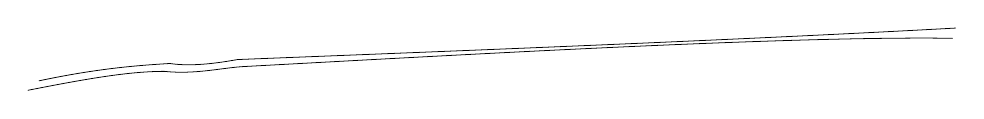
\begin{tikzpicture}[x=1cm,y=1cm,line cap=round]
\draw[line width=.28pt] (0,0) .. controls (.80,.17) and (1.34,.20) .. (1.66,.22)
 .. controls (1.93,.18) and (2.24,.22) .. (2.52,.27)
 .. controls (5.05,.37) and (8.73,.51) .. (11.64,.67);
\draw[line width=.28pt] (-.14,-.12) .. controls (.67,.04) and (1.17,.12) .. (1.59,.12)
 .. controls (1.98,.08) and (2.29,.16) .. (2.58,.18)
 .. controls (5.54,.34) and (9.54,.57) .. (11.60,.54);
\end{tikzpicture}}

\margin{\uline{NB} (10) s'écrit aussi \deleted{\unsure{(11)}}
\[
(10\text{ bis})\qquad
(\ell_0^{\gamma}h_0^{-1})\cdot\rho(\ell_0^{\gamma}h_0^{-1})\cdot\rho^2(\ell_0^{\gamma}h_0^{-1})=1
\]
}
\scanpage{59}
\mspage{318}

\[
(11)\qquad
\left\{
\begin{aligned}
u(\ell_0)&=\operatorname{int}(g_0)(\ell_0^p)\\
u(\ell_1)&=\operatorname{int}\bigl(\underbrace{\sigma_\infty(g_0)}_{\inserted{\unsure{g_1}}}\bigr)(\ell_1^p)\\
u(\ell_\infty)&=\operatorname{int}\bigl(g_0\ell_0^{-\unsure{\gamma|\sigma}}\rho^{-1}(h_0)\bigr)(\ell_\infty^p)
\end{aligned}
\right.,
\]

et il faut en toute rigueur, en plus des conditions (9),(10), exiger que les deux éléments $u(\ell_0),u(\ell_1)$ \inserted{donnés par (11)} \unsure{forment} des générateurs du groupe profini $\widehat{\Pi}_{0,3}$.
\margin{(11 bis)}

Je vais calculer l'action de $u$ sur $\widehat{\mathfrak S}_{0,3}^{+}$, en considérant ce groupe comme engendré par les éléments
\[
(12)\qquad \ell'_1=\sigma_\infty,\qquad \ell'_\infty=\rho^{-1}
\]
donc il faut calculer simplement \inserted{$\operatorname{int}(u).\sigma_\infty=u(\sigma_\infty)=$} $u\sigma_\infty u^{-1}$ et $u(\rho)=\operatorname{int}(u).\rho=u\rho u^{-1}$. On a par construction ($u$ \unsure{commutant} à $\sigma_\infty$)
\[
(13)\qquad u\unsure{\circ}\sigma_\infty u^{-1}=\sigma_\infty,
\]
et d'autre part on vérifie que
\[
\deleted{u(\rho)=u\rho u^{-1}=\operatorname{int}(h}
\]
\[
(14)\qquad \deleted{u\rho}\quad
\left\{
\begin{aligned}
\rho^{-1}u\rho&=\operatorname{int}(h)u\\
\inserted{\text{avec}}\quad h&=(\rho^{-1}\sigma_\infty)(g_0)\ell_0^{\gamma}g_0^{-1}
\end{aligned}
\right.
\]
\margin{i.e. $u\rho u^{-1}=\rho\operatorname{int}(h).$\\
$=\operatorname{int}(\rho(h))\rho$\\
i.e. $\rho(h)=\sigma_\infty(g_0)\ell_1^{\gamma}\rho(g_0)^{-1}$}

donc on trouve, en \unsure{termes} d'une opération sur le groupe $\widehat{\mathfrak S}_{0,3}^{+}$ engendré par \inserted{$\ell'_1=$}$\sigma_\infty$ et \inserted{$\ell'_\infty=$}$\rho^{-1}$ (ou $\rho$)
\[
(15)\qquad
\left\{
\begin{aligned}
u(\sigma_\infty)&=\sigma_\infty\\
u(\rho)&=g.\rho
\end{aligned}
\right.
\quad\inserted{\text{avec}}\quad
 g=\sigma_\infty(g_0)\ell_1^{\unsure{\gamma|\tau}}\rho(g_0)^{-1}
\]
\scanpage{60}

\uline{NB} La relation \deleted{$u(\rho)^3=1$} $u(\sigma_\infty)^2=1$ est triviale, la relation $u(\rho)^3=1$ se réduit à
\[
\deleted{g\rho(g)\unsure{=}}
\]
\[
(16)\qquad g\rho(g)\rho^2(g)=1
\]
qui est conséquence de l'expression explicite (15) de $g$, et de la formule (10).

Notons qu'on \deleted{\unsure{aura}} \inserted{devrait avoir}, \& \unsure{reprenant}
\[
\ell'_0=\sigma_\infty\rho=\unsure{\varepsilon_0|e_0}\qquad
(\text{\unsure{d'où}}\quad \ell_0^{\prime 2}=\ell_0)
\]
\[
(17)\qquad
u(\unsure{\ell'_0})
=\operatorname{int}(g_0)(\ell_0^{\prime p})
\]
\inserted{\figure{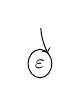
\begin{tikzpicture}[x=1cm,y=1cm,baseline=-0.45ex,line width=0.35pt]
\draw[->] (0.01,0.45) .. controls (0.02,0.31) and (0.06,0.22) .. (0.10,0.13);
\draw (0,0) ellipse [x radius=0.15cm,y radius=0.18cm];
\node[inner sep=0pt] at (0,-0.01) {$\scriptstyle\unsure{\varepsilon}$};
\end{tikzpicture}}}
\margin{?}
--- cette relation \unsure{au|en} carré n'est autre que la première relation (11)
\[
u(\ell_0)=\operatorname{int}(g_0)(\ell_0^p).
\]

[La relation (17) en est une conséquence, si on admet que le centralisateur de $L_0=\ell_0^{\widehat{\mathbb Z}}$ dans $\widehat{\Pi}_{0,3}$ est réduit à $L_0$\ldots]

On devrait avoir aussi la relation
\[
(18)\qquad u(\rho)\deleted{\unsure{\equiv|=}}\inserted{\text{conjugué de}}\rho^p
\quad\deleted{\text{\unsure{mod|modulo}}\ \widehat{\Pi}_{0,3}}
\]
\deleted{\illegible{1}} sur laquelle nous \unsure{allons} revenir -- il n'est pas clair pour moi qu'elle soit conséquence des conditions \unsure{envisagées} sur $u$ jusqu'à présent.
\margin{\deleted{\illegible{2}}}
% ===== LM_P065: second pass, checked against the scans =====
\scanpage{61}
\mspage{319}

Considérons maintenant l'hom \unsure{(3)}
\[
\tag{18}
\left\{
\begin{aligned}
\widehat\varphi:\quad &\widehat\Pi_{0,3}\longrightarrow
  \widehat{\mathfrak S}_{0,3}^{+}\\
&\ell_0\longmapsto\ell'_0=\sigma_\infty\rho=\varepsilon_0\\
&\ell_1\longrightarrow\ell'_1=\sigma_\infty\\
&\ell_\infty\longmapsto\ell'_\infty=\rho^{-1}
\end{aligned}
\right.
\]
et écrivons qu'il commute, \unsure{en tant} qu'hom. ext., à $u$.
Cela signifie donc qu'il existe un
\[
\tag{19}
\lambda\in\widehat{\mathfrak S}_{0,3}^{+}
\]
tel que l'on ait
\[
\tag{20}
\widehat\varphi(\unsure{ux})=\lambda\,u\widehat\varphi(x)\,\lambda^{-1}
\qquad \forall x\in\widehat\Pi_{0,3},
\]
et il suffit d'exprimer cette condition pour $x$ égal à l'un des deux
gén. $\ell_0,\ell_1$ de $\widehat\Pi_{0,3}$

Pour $x=\ell_0$ la relation (20) s'écrit
\[
\tag{21}
u(\ell'_0)=\operatorname{int}(\lambda^{-1}\widehat\varphi(g_0))(\ell_0'{}^{p})
\]
ce qui, comparé avec (17), donne
\[
\operatorname{int}(g_0^{-1}\lambda^{-1}\widehat\varphi(g_0))(\ell_0'{}^{p})
=\ell_0'{}^{p}\quad\text{donc}
\]
\[
\deleted{(22)}\qquad
g_0^{-1}\lambda^{-1}\widehat\varphi(g_0)=\ell_0'{}^{\beta}
\qquad(\beta\in\widehat{\mathbb Z})
\]
ou encore
\[
\tag{22}
\boxed{\lambda=\widehat\varphi(g_0)\ell_0'{}^{-\beta}g_0^{-1}}
\inserted{=\widehat\varphi(g_0h_0^{-1})=\widehat\varphi(\sigma_\infty(g_0))}
\]
\margin{$\searrow$ \unsure{cf} plus bas (24 bis)}

Pour $x=\ell_1$ la relation (20) s'écrit
\scanpage{62}

\[
\tag{23}
u(\ell'_1)=\operatorname{int}(\lambda^{-1}\widehat\varphi(g_1))(\ell_1'{}^{p})
\]
\margin{où $(g_1=\sigma_\infty(g_0)=\sigma_\infty g_0\sigma_\infty\unsure{)}$}
ou encore
\[
\sigma_\infty=\operatorname{int}(\lambda^{-1}\widehat\varphi(g_1))(\sigma_\infty)
\]
\margin{Car $\sigma_\infty^{p}=\sigma_\infty$ car
\inserted{$\sigma_\infty^2=1$ et} \unsure{l'image} de $p$ dans
$(\mathbb Z/2\mathbb Z)^*$ est $1$ !}
ou encore $\sigma_\infty$ commute à
\[
\lambda^{-1}\widehat\varphi(g_1)
\overset{\inserted{\text{cf (22)}}}{=}
g_0\ell_0'{}^{\beta}\widehat\varphi
 \bigl(\underbrace{g_0^{-1}\sigma_\infty(g_0)}_{h_0^{-1}}\bigr)
=g_0\ell_0'{}^{\beta}\widehat\varphi(h_0^{-1})
\]
ou encore à son inverse $\widehat\varphi(h_0)\ell_0'{}^{-\beta}g_0^{-1}$
ce qui s'écrit aussi
\[
\underbrace{\sigma_\infty
 \bigl(\widehat\varphi(h_0).\ell_0'{}^{-\beta}.g_0^{-1}\bigr)}
=\widehat\varphi(h_0).\ell_0'{}^{-\beta}.g_0^{-1}
\]
\[
\sigma_\infty(\widehat\varphi(h_0)).
\underbrace{\varepsilon_1^{-\beta}}_{(\rho\sigma_\infty)^{-\beta}}.
\sigma_\infty(g_0)^{-1}
=\widehat\varphi(h_0)\ell_0'{}^{-\beta}g_0^{-1}
\]
\[
\sigma_\infty(\widehat\varphi(h_0))
 (\underbrace{\rho\sigma_\infty}_{\varepsilon_1})^{-\beta}h_0
=\widehat\varphi(h_0).\varepsilon_0^{-\beta}
\]
\[
\tag{24}
\boxed{
\overbrace{\varepsilon_1^{-\beta}h_0\varepsilon_0^{\beta}}
 ^{\inserted{\sigma_\infty(g_0\varepsilon_0^{\beta})^{-1}(g_0\varepsilon_0^{\beta})}}
=\sigma_\infty(\widehat\varphi(h_0))^{-1}\widehat\varphi(h_0)
}
\]
\margin{\unsure{Correct?} $\searrow$}
\margin{\uline{NB.} Si $g_0$ est remplacé par
\inserted{$g'_0=$} $g_0\ell_0^{\lambda}$ $(\lambda\in\widehat{\mathbb Z})$,
$h_0$ est remplacé par $h'_0=\ell_1^{-\lambda}\unsure{h_0|g_0}\ell_0^{\lambda}$,
et on \unsure{trouve} que $\beta$ \unsure{est} \unsure{''} remplacé par
$\beta'=\beta-3\lambda$.
Ceci montre \inserted{?} qu'on peut de \uline{façon unique}
\illegible{1} \uline{normaliser} le choix de $g_0$, de telle façon que l'on ait
$\beta\in\{0,1,2\}$.
(Il faudrait élucider si $\beta$ prend effectivement toutes les
\unsure{trois} valeurs mod $3$\ldots)}
\margin{\uuline{NB} Cette équation équivaut à l'équation
\uline{plus simple}
\[
\text{(24 bis)}\qquad
\boxed{\widehat\varphi(h_0)=\sigma_\infty^{\unsure{\varepsilon}}g_0\varepsilon_0^{\beta}}
\]}
\[
\unsure{(25)}\qquad
\left\{
\begin{aligned}
&h_0\text{ donné par (8) en fonction de }g_0\\
&\varepsilon_0=\ell'_0=\sigma_\infty\rho
   &&(\varepsilon_0^2=\ell_0)\\
&\varepsilon_1=\rho\sigma_\infty=\sigma_0\rho
   &&(\varepsilon_1^2=\ell_1)
\end{aligned}
\right.
\]

Posant, pour $\deleted{\unsure{g}}\ \mu\in
\widehat{\mathfrak S}_{0,3}^{+}$,
\[
\tag{26}
\widetilde\mu=\sigma_\infty(\mu)^{-1}\mu
=\sigma_\infty\mu^{-1}\sigma_\infty\mu=[\sigma_\infty,\mu]
\]
(de sorte que $h_0=\widetilde g_0$) la formule \unsure{(24)|(25)} prend la forme
\[
\tag{27}
\varepsilon_1^{-\beta}\unsure{\widetilde g_0}\varepsilon_0^\beta
=\bigl(\widehat\varphi(\widetilde g_0)\bigr)^{\sim}.
\]
\scanpage{63}
\mspage{320}

En résumé :

\uline{Proposition} Considérons un autom ext. $u$ du groupe à lacets
$\widehat\Pi_{0,3}$, réalisé par $g_0\in\widehat\Pi_{0,3}$
\inserted{mod $L_0$,}
et $p\in\widehat{\mathbb Z}^{*}$,
(et $\gamma\in\widehat{\mathbb Z}^{*}$ uniquement déterminé
\unsure{par termes|en termes} de $g_0$ et $p$)
par les formules (11), au moyen d'un autom effectif
\inserted{(noté encore $u$)} qui commute à $\sigma_\infty$ ---
les données $g_0,p$ (et $\gamma$) \unsure{étant} \inserted{donc}
assujetties à vérifier les conditions (9) et (10) ci-dessus,
plus la condition d'engendrement (11 bis).
\inserted{(On prolonge $u$ \unsure{en} autom de
$\widehat{\mathfrak S}_{0,3}^{+}$
par $\operatorname{int}(u)$, cf (15))}
Pour que l'hom extérieur
$\widehat\varphi:\widehat\Pi_{0,3}\longrightarrow
\widehat{\mathfrak S}_{0,3}^{+}$
défini par (18) commute à l'action ext. de $u$,
il f. et s. que l'on puisse trouver un $\beta\in\widehat{\mathbb Z}$,
tel qu'on ait (24), ou ce qui revient au $\overline{\mathrm m}$, (27),
\margin{\unsure{mieux :} \uuline{24 bis}}

Cette condition \inserted{(pour $\beta$ fixé)} équivaut aussi à la formule
(20) pour $x=\ell_\infty$ ($\lambda$ \unsure{étant} tjrs donné par (22)),
\deleted{\unsure{(2}} i.e. à la formule
\[
\tag{28}
u(\ell'_\infty)=\operatorname{int}(\lambda^{-1}\widehat\varphi(g_\infty))
 (\ell_\infty'{}^p),\qquad\text{où}
\]
\[
\tag{29}
g_\infty=g_0\ell_0^{-\gamma}\rho^{-1}(h_0)
\qquad(\text{et }\lambda\text{ donné par (22)}).
\]
\scanpage{64}

formule qui précise donc la formule \unsure{présomptive} (18). Elle s'écrit aussi, plus explicitement
\[
\rho^{-1}g^{-1}
=\operatorname{int}\bigl(g_0\varepsilon_0^{\beta}
\widehat\varphi(\ell_0^{\gamma}\rho^{-1}(h_0))\bigr)
(\rho^{-p})
\]
\inserted{\[
g_0\varepsilon_0^{\beta+\gamma}\widehat\varphi(\rho^{-1}(h_0))
\]}
i.e. (en prenant les inverses, et explicitant $g$)
\[
(30)\qquad
\boxed{
\deleted{\illegible{1}}\inserted{h_0^{-1}\ell_1^{\gamma}\rho}
=\operatorname{int}\bigl(
\deleted{\unsure{g_0}}\varepsilon_0^{\deleted{\unsure{\beta+\gamma}}\inserted{\alpha}}
\widehat\varphi(\rho^{-1}(h_0))\bigr)
(\rho^{p\deleted{\unsure{-p}}})
}
\]
\margin{\uline{NB} On pose $\alpha=\beta+\gamma$. L'existence \unsure{de} $\beta\in\widehat{\mathbb Z}$ vérifiant (24), équivaut à celle \unsure{de} $\alpha\in\widehat{\mathbb Z}$ vérifiant (30).}

L'équivalence de (24) et (30) peut paraître un peu étrange, du fait \inserted{p.ex.} que dans (24) l'exposant $p$ n'intervient pas explicitement, mais seulement $h_0$, tandis que la formule (30) fait intervenir la valeur de $p\in\widehat{\mathbb Z}^{*}$ mod $3$ (qui donne $\rho^p=\rho$ ou $\rho^p=\rho^{-1}$). Mais en tout état de cause, que ce soit sous la forme (24) \unsure{où|ou} sous la forme (30), il semble bien que la condition en question soit hautement non tautologique !

Pour bien faire, il faudrait \unsure{d'abord} expliciter les conditions congruentielles du \S~39 en fonction de $g_0,p$.
\scanpage{65}
\mspage{321}

Je voudrais \unsure{comparer} les autom. ext. de $\widehat\Pi_{0,3}$, et ceux de $\widehat{\mathfrak S}_{0,3}^{+}$, tenant compte de la suite exacte
\[
(31)\qquad
\diagram{\begin{tikzcd}[ampersand replacement=\&]
1\arrow[r,no head]\&\widehat\Pi_{0,3}\arrow[r,no head]\&
\widehat{\mathfrak S}_{0,3}^{+}\arrow[r]\arrow[d,draw=none,"{\inserted{\unsure{\wr}}}" description]\&
\mathfrak S_{3}\arrow[r,no head]\&1\\
\&\&\inserted{\widehat{\Pi'}_{0,3}}
\end{tikzcd}}
\]

\deleted{\uline{Proposition}} \inserted{Notons} que tt autom. ext. \inserted{$u$} de $\widehat{\mathfrak S}_{0,3}^{+}$ qui \unsure{invarie} le sous-groupe distingué $\widehat\Pi_{0,3}$, et induit dans le quotient $\mathfrak S_{3}$ un autom. extérieur trivial, peut s'écrire comme déduit d'un autom. \inserted{$u_0$} de $\widehat{\mathfrak S}_{0,3}^{+}$, \unsure{stabilisant} $\widehat\Pi_{0,3}$, et induisant l'\uline{identité} sur le quotient $\mathfrak S_{3}$ --- et $u_0$ est alors déterminé mod composition avec un élément $\operatorname{int}(g)$, où $g\in\widehat{\mathfrak S}_{0,3}^{+}$ \unsure{est} tel que son image dans $\mathfrak S_{3}$ soit central, i.e. $=1$, i.e. $g\in\widehat\Pi_{0,3}$. Donc
\[
(32)\qquad
\begin{gathered}
\text{groupe des automorphismes}\\
\text{ext. de $\widehat{\mathfrak S}_{0,3}^{+}$ qui}\\
\text{induisent dans $\mathfrak S_{3}$ un autom.}\\
\text{ext. trivial (donc \unsure{invarient}}\\
\widehat\Pi_{0,3})
\end{gathered}
\simeq
\begin{gathered}
\text{groupe des}\\
\text{autom. de}\\
\widehat{\mathfrak S}_{0,3}^{+}\text{ qui}\\
\text{induisent}\\
\text{l'identité dans}\\
\text{son quotient $\mathfrak S_{3}$,}\\
\text{\uline{mod} le sous-}\\
\text{groupe des}\\
\text{autom. int.}\\
\text{par des $g\in\widehat\Pi_{0,3}$}
\end{gathered}
\]
\scanpage{66}

Un \inserted{tel} autom $u_0$ est-il connu par sa restriction à $\widehat\Pi_{0,3}$ ? En d'autres termes, un autom. de $\widehat{\mathfrak S}_{0,3}^{+}$ \deleted{qui} ($\simeq\mathrm{Sl}(\unsure{2|1},\mathbb Z)^{\unsure{\prime}\wedge}$) qui induit l'identité sur $\widehat\Pi_{0,3}$ et sur $\mathfrak S_{3}$, est-il trivial ? Il suffit de prouver que sa restriction à l'image inverse \inserted{$\widehat\Pi_{\unsure{0,\infty|0,3}}\cdot\{1,\unsure{\sigma_\infty}\}$} de $\{1,\dot\sigma_\infty\}\subset\mathfrak S_{3}$ est \unsure{trivial|triviale} (par symétrie ce sera aussi le cas en remplaçant $\dot\sigma_\infty$ par $\dot\sigma_0,\dot\sigma_1$, or ces trois sous groupes engendrent $\widehat{\mathfrak S}_{0,3}^{+}$. On aura $f(\sigma_\infty)=\sigma_\infty g$, avec $g\in\widehat\Pi_{0,3}$ [et on doit avoir $\sigma_\infty g\sigma_\infty g=1$ i.e.
\[
g\cdot\sigma_\infty(g)=1
\]
]
de plus \deleted{pour $x\in\Pi_{0,3}$ \unsure{on a}} \inserted{on devra avoir que}
\[
\operatorname{int}(\sigma_\infty g)\vert\widehat\Pi_{0,3}
=\deleted{\unsure{f(x\sigma_\infty)}}\operatorname{int}(\sigma_\infty)\vert\widehat\Pi_{0,3}
\]
d'où \deleted{$g\in$}
\[
\operatorname{int}(g)\vert\widehat\Pi_{0,3}=\mathrm{id}
\quad\text{i.e.}\quad
g\in\unsure{\operatorname{Centre}}(\widehat\Pi_{0,3})
\quad\text{i.e.}\quad g=1,
\]
OK.

Mais à quelle condition un autom. de $\widehat\Pi_{0,3}$ \deleted{peut} se prolonge-t-il en un autom. de $\widehat{\mathfrak S}_{0,3}^{+}$ qui \deleted{soit}\inserted{\unsure{induise}} l'identité sur $\mathfrak S_{3}$ ? On voit aussitôt qu'il \uline{faut} pour ceci que l'autom. ext. de $\widehat\Pi_{0,3}$ qu'il induit commute à l'action de $\mathfrak S_{3}$.
\scanpage{67}
\mspage{\unsure{322|332}}

C'est suffisant, car soit $\Gamma\inserted{{}\subset\mathrm{Aut\,ext}(\widehat{\Pi}_{0,3})}$ le groupe des autom.
ext. de $\widehat{\Pi}_{0,3}$ qui ont cette propriété (on ne
se préoccupe pas pour le moment de la
structure à lacets de $\widehat{\Pi}_{0,3}$), on a
$\Gamma\cap\mathfrak S_3=(1)$ (en identifiant $\mathfrak S_3$ à un
\unsure{ss-groupe} de $\mathrm{Aut\,ext}\,\widehat{\Pi}_{0,3}$) car \deleted{\unsure{\mathfrak S}} le centre
de $\mathfrak S_3$ est trivial, donc
\margin{ceci est \unsure{évident|évidemment}}
\[
\deleted{\unsure{\Gamma\times}}\ \mathfrak S_3\times\Gamma\hookrightarrow\mathrm{Autext}(\widehat{\Pi}_{0,3}),
\]
et on a donc une structure d'extension
\[
1\unsure{\longrightarrow}\widehat{\Pi}_{0,3}\longrightarrow\mathcal E\longrightarrow\mathfrak S_3\times\Gamma\longrightarrow1
\tag{33}
\]
(car le centre de $\widehat{\Pi}_{0,3}$ est trivial), ou encore
une structure d'extension
\[
1\longrightarrow\widehat{\mathfrak S}_{0,3}^{+}\unsure{\longrightarrow}\mathcal E\longrightarrow\Gamma\longrightarrow1
\tag{34}
\]
qui définit une action extérieure de $\Gamma$
sur $\widehat{\mathfrak S}_{0,3}^{+}$ --- qui est l'action ext.
cherchée. Ainsi

\uline{Prop} le groupe des autom. ext. de $\widehat{\Pi}_{0,3}$ qui
\unsure{commutent} à $\mathfrak S_3$ est isom. can. au groupe
des autom. ext. de $\widehat{\mathfrak S}_{0,3}^{+}$ qui induisent
dans $\mathfrak S_3$ l'autom. ext. trivial.
\margin{Mais \uline{tout} autom. de $\mathfrak S_3$ est intérieur !}
\scanpage{68}

\uline{Corollaire} le groupe des autom. de $\widehat{\Pi}_{0,3}$ qui
commutent extérieurement à $\mathfrak S_3$, est isom.
au groupe des autom. de $\widehat{\mathfrak S}_{0,3}^{+}$ qui
induisent sur $\mathfrak S_3$ l'autom. triviale (par
restriction de ces derniers)

\uuline{Corollaire}
\[
\diagram{\begin{tikzcd}[ampersand replacement=\&,column sep=small,row sep=large]
1 \arrow[r,no head]
\& \widehat{\Pi}_{0,3} \arrow[r]
\& \mathrm{Aut}\left(\widehat{\Pi}_{0,3}\,\middle|\,
  \begin{array}{l}\mathrm{comm.}\\\mathrm{ext.}^{\unsure{t}}\\\text{à }\mathfrak S_3\end{array}\right) \arrow[r]
\& \mathrm{Autext}\left(\widehat{\Pi}_{0,3}\,\middle|\,
  \begin{array}{l}\mathrm{comm.}\\\text{à }\mathfrak S_3\end{array}\right) \arrow[r]
\& 1
\\
1 \arrow[r,no head]
\& \widehat{\Pi}_{0,3} \arrow[r,no head] \arrow[u,phantom,"{\text{''}}" description]
\& \underbrace{\mathrm{Aut}\left(\widehat{\mathfrak S}_{0,3}^{+}\,\middle|\,
  \begin{array}{l}\text{id. sur le}\\\text{quotient }\mathfrak S_3\end{array}\right)}_{\mathcal E^{!}}
  \arrow[r] \arrow[u,"{\sim\ \text{\unsure{restr.} à }\widehat{\Pi}_{0,3}}"]
\& \mathrm{Autext}\left(\widehat{\mathfrak S}_{0,3}^{+}\,\middle|\,
  \begin{array}{l}\text{\deleted{\unsure{finie}}\inserted{\unsure{trivial}}}\\\text{sur le}\\\text{quotient }\mathfrak S_3\end{array}\right)
  \arrow[r] \arrow[u,"\sim"]
\& \unsure{1}
\end{tikzcd}}
\tag{35}
\]

\deleted{\uline{Corollaire}
Soit $u\in\mathrm{Aut}\deleted{\mathrm{ext}}(\widehat{\mathfrak S}_{0,3}^{+})$, \unsure{induisant}
\unsure{Soit} \illegible{1} $u\in\mathrm{Aut}(\widehat{\mathfrak S}_{0,3}^{+})$ et $\unsure{u_0}\unsure{=|:=}u|\widehat{\Pi}_{0,3}$
\margin{dans $\mathcal E$}
l'autom. \inserted{ext.} trivial sur $\mathfrak S_3$. On a donc
\unsure{commutant} \illegible{2}
\[
u(\sigma_\infty)=g\sigma_\infty\quad\text{avec}\quad g\in\widehat{\Pi}_{0,3}\quad\text{\unsure{bien} déterminé},
\]
on a \illegible{1} que $\sigma_\infty$
et $(g\sigma_\infty)^2=1$ i.e. $g\sigma_\infty g\sigma_\infty=1$ i.e. $g\sigma_\infty g$.}

Cette extension $\mathcal E^{!}$ de $\Gamma$ par $\widehat{\Pi}_{0,3}$ est
scindée\inserted{\unsure{non canoniquement}}, le sous-groupe \unsure{splittant|splitting} est formé
des autom. de $\widehat{\Pi}_{0,3}$ qui commutent à $\sigma_\infty$,
ou encore les autom. de $\widehat{\mathfrak S}_{0,3}^{+}$ qui
\deleted{\unsure{commutent}}\inserted{fixent} \unsure{à} $\sigma_\infty$ (et \inserted{qui fixent} $\rho\ \mathrm{mod}\ \widehat{\Pi}_{0,3}$)
\margin{provient du fait qu'il \deleted{\illegible{2}} \inserted{\unsure{existe}} \deleted{\illegible{1}} \unsure{un} \illegible{2} \inserted{$\widehat{\Pi}_{0,3}$-\unsure{conj.}} \illegible{1} d'ordre $2$ au dessus de $\sigma_\infty$ \ldots}
\[
\left\{
\begin{aligned}
u(\sigma_\infty)&=\sigma_\infty\\
u(\rho)&=g.\rho
\end{aligned}
\right.
\qquad(g\in\widehat{\Pi}_{0,3})
\tag{36}
\]
\scanpage{69}
\mspage{323}

\unsure{écrivant} que $u$ est un \unsure{endom.} (car on \unsure{se rappelle}
que $\widehat{\mathfrak S}_{0,3}^{+}$ est défini par les gén. $\sigma_\infty,\rho$
avec les relations
\begin{equation}
\sigma_\infty^2=\rho^3=1
\tag{37}
\end{equation}
\unsure{on trouve} la condition
\begin{equation}
(g\rho)^3=1\qquad\text{i.e.}\qquad g\,\rho(g)\,\rho^2(g)=1.
\tag{38}
\end{equation}

\margin{de plus il \unsure{faut} pour que $\sigma_\infty$ et $g\rho$
\unsure{engendrent} $\unsure{\widehat\Pi_{0,3}}$, avec seules relations
$\sigma_\infty^{\unsure{2}}=(g\rho)^3=1$.}

\uline{Corollaire}. Soit $u\in\mathcal E^{!}$ un autom. de
$\widehat{\mathfrak S}_{0,3}^{+}$ qui induit l'identité sur $\mathfrak S_3$.
Conditions équivalentes:

a) $\exists\ p\in\widehat{\mathbb Z}^{*}$ tel que
$u(\underset{\varepsilon_0}{\uline{\ell'_0}})$ conjugué dans
$\widehat{\mathfrak S}_{0,3}^{+}$ à $\ell_0'{}^p$
(ce $p$ est alors unique\inserted{, et on peut conjuguer par un \unsure{élément} de $\widehat\Pi_{0,3}$}).

b) $\exists\ p\in\widehat{\mathbb Z}^{*}$ tel que $u(\ell_0)$ soit conjugué dans
$\widehat\Pi_{0,3}$ à $\ell_0^p$ (ce $p$ est alors unique).

c) $u_0\overset{\mathrm{dfn}}{=}u\mid\widehat\Pi_{0,3}$ respecte la structure à lacets de $\widehat\Pi_{0,3}$.

De plus, le $p$ dans a) et b) est le $\overline{\mathrm m}$.

\uline{\unsure{Dém}}. Si $u(\ell'_0)=\operatorname{int}(g_0)(\ell_0'{}^p)$, avec
$g_0\in\widehat{\mathfrak S}_{0,3}^{+}$,
élevant au carré on \unsure{aura} $u(\ell_0)=\operatorname{int}(g_0)(\ell_0^p)$,
cela montre que l'image $\dot g_0$ de $g_0$ dans $\mathfrak S_3$
\unsure{invarie} $0$ i.e. est \deleted{\illegible{1}} $1$ ou $\dot\sigma_0$,
\deleted{donc} si c'est $1$ on a bien b), sinon on \unsure{met|\deleted{sait q}}
$g_0=h\sigma_0$ \inserted{($h\in\widehat\Pi_{0,3}$)}
\deleted{\unsure{d'où}}
\[
u(\ell_0)=\operatorname{int}(h)\,
\underset{(\sigma_0(\ell_0))^p}{\uline{\sigma_0(\ell_0^p)}}
\]
or on sait que $\sigma_0(\ell_0)=\operatorname{int}(a)\ell_0$
\inserted{(avec $a\in\widehat\Pi_{0,3}$)},
\inserted{d'où $\sigma_0(\ell_0)^p=\operatorname{int}(a)\ell_0^p$},
donc $u(\ell_0)=\operatorname{int}(ha)(\ell_0^p)$, d'où b) avec le $\overline{\mathrm m}$ $p$.
\scanpage{70}

Comme on sait l'unicité de $p$ dans b), dans a) aussi. Si on a
\begin{equation}
u_0(\ell_0)=\operatorname{int}(g_0)(\ell_0^p)
\qquad (g_0\in\widehat\Pi_{0,3})
\tag{39}
\end{equation}
on en déduit, écrivant
\[
\deleted{\rho u_0\rho^{-1}(\ell_0)\unsure{=}}
\qquad
\rho u_0\rho^{-1}=\operatorname{int}(g^{-1})u_0
\qquad (\unsure{a|g}\in\widehat\Pi_{0,3})
\]
\[
\deleted{u_0 \ell_1}
\]
\[
u_0(\ell_1)=\operatorname{int}(\unsure{a|g})
\underbrace{\rho\underbrace{u_0\underbrace{\rho^{-1}(\ell_1)}_{\ell_0}}_{
\operatorname{int}(g_0)(\ell_0^p)}}_{
\operatorname{int}(\rho(g_0))(\ell_1^p)}
=\operatorname{int}(g\rho(g_0))(\ell_1^p)
\]
i.e.
\begin{equation}
u_0(\ell_1)=\operatorname{int}(g_1)(\ell_1^p)
\qquad\text{avec}\quad g_1=g\rho(g_0)
\tag{40}
\end{equation}
et de $\overline{\mathrm m}$
\begin{equation}
\unsure{u_0|u}(\ell_\infty)=\operatorname{int}(g_\infty)(\ell_\infty^p)
\qquad\text{avec}\quad
\begin{aligned}
g_\infty&=g\rho(g_1)\\
&=g\rho(g)\rho^2(g_0)
\end{aligned}
\tag{41}
\end{equation}
donc b) $\Rightarrow$ c). Enfin \unsure{prouvons} c) $\Rightarrow$ a).

On a par hypothèse
\[
\begin{array}{rcl}
u_0(\ell_0)&=&\operatorname{int}(g)\ell_0^p\\
\text{''}&&\text{''}\\
u(\varepsilon_0)^2&&
\operatorname{int}(g)(\unsure{\ell|\varepsilon}_0^{\unsure{2p|p}})^2
=(\operatorname{int}g(\unsure{\ell_0^p|\varepsilon_0^p}))^2
\end{array}
\]
je dis qu'on a alors
\[
u(\varepsilon_0)=\operatorname{int}(g)(\varepsilon_0^p).
\]
Il suffit de \deleted{voir}\inserted{\unsure{se rappeler}} que
\deleted{\unsure{tt}}\inserted{le seul} \unsure{élément} de
$\widehat{\mathfrak S}_{0,3}^{+}$ de carré égal à $\ell_0$ est $\varepsilon_0$\ldots\quad OK

\margin{\unsure{vérifier}}
% ===== LM_P066: second pass, checked against the scans =====
\scanpage{71}
\mspage{324}

\deleted{On doit donc \unsure{avoir}}

\unsure{Désormais} nous nous \unsure{bornons} aux autom.
(\inserted{\unsure{eff. ou}} extérieurs) de $\widehat{\Pi}_{0,3}$
qui \unsure{respectent} la str. à lacets, et \unsure{commutent} à
$\mathfrak S_3$ (extérieurement)
--- qui \unsure{correspondent} aux autom.
\inserted{(\unsure{eff. ou ext.})} de
$\widehat{\mathfrak S}_{0,3}^{+}$ qui \unsure{induisent}
l'identité sur $\mathfrak S_3$,
et \unsure{satisfont} a) ci-dessus. \deleted{Ils \illegible{1}}

Les \unsure{autom.} \uline{extérieurs} de cette nature
\unsure{correspondent} donc aux aut. effectifs $u$
\inserted{de $\widehat{\Pi}_{0,3}$}
qui \unsure{commutent} à $\sigma_\infty$, i.e. $u$
\inserted{de $\widehat{\mathfrak S}_{0,3}^{+}$} qui
\unsure{fixent} $\sigma_\infty$, et sont déterminés par un
$g\in\widehat{\Pi}_{0,3}$ satisfaisant (38), \uline{et} tel que
de plus il existe \inserted{$p\in\widehat{\mathbb Z}^{*}$ et}
$g_0\in\widehat{\Pi}_{0,3}$ satisfaisant
\[
(39)\qquad
u(\ell'_0)=\operatorname{int}(g_0)({\ell'_0}^{p})
\qquad\text{i.e.}\qquad
u(\ell_0)=\operatorname{int}(g_0)(\ell_0^{p})
\]
(\unsure{où|i.e.} $g_0$ est déterminé mod $L_0=\ell_0^{\widehat{\mathbb Z}}$
\unsure{\ldots}). Des calculs faits par ailleurs \unsure{montrent}
\inserted{alors} qu'on doit avoir
\[
(40)\qquad g=\sigma_\infty(g_0)\,\ell_1^{\gamma}\,\rho(g_0)^{-1}
\]
\margin{avec $\gamma\in\widehat{\mathbb Z}$ bien déterminé
(\unsure{indépendant} du choix de $g_0$)}
i.e.
\[
(41)\qquad
\deleted{\rho(g_0)}\,\sigma_\infty(g_0)^{-1}\,
\underbrace{g\rho(g_0)}_{\unsure{g_1}}\in L_1
=\unsure{\mathcal N|N|\mathrm{Norm}}_{\widehat{\Pi}_{0,3}}(L_1)
\]
\scanpage{72}

En effet, on a par \unsure{hyp.} sur $g_0$ (cf (39))
\[
(42)\qquad u(L_0)=\operatorname{int}(g_0)(L_0)
\]
\unsure{\deleted{d'où}|d'où}
\[
\begin{aligned}
&u\sigma_\infty(L_0)=u(L_1)\overset{40}{=}
  \operatorname{int}(g_1)(L_1)\\
&\Vert\quad(\text{car }u\sigma_\infty=\sigma_\infty u)\\
&\sigma_\infty u(L_0)\underset{(42)}{=}
 \sigma_\infty(\operatorname{int}(g_0)(L_0))
 =\operatorname{int}(\sigma_\infty(g_0))(\sigma_\infty(L_0))
 =\operatorname{int}(\sigma_\infty(g_0))(L_1)
\end{aligned}
\]
d'où
\[
\operatorname{int}(\sigma_\infty(g_0)^{-1}g_1)(L_1)\subset L_1
\]
donc
\[
\sigma_\infty(g_0)^{-1}\underbrace{g_1}_{g\rho(g_0)}
\in \mathcal N_{\widehat{\Pi}_{0,3}}(L_1)=L_1
\]
d'où
\[
\sigma_\infty(g_0)^{-1}\unsure{g_1|g}\rho(g_0)=\ell_1^\gamma
\qquad (\gamma\in\widehat{\mathbb Z})
\]
d'où (40). On notera, pour \unsure{y revenir}, que l'élément $g$
défini en termes d'un $g_0$ \inserted{et de $\gamma$} \margin{$\checkmark$}
ne dépend en effet que de $g_0$ mod $L_0$. \deleted{\illegible{1}}

\margin{\figure{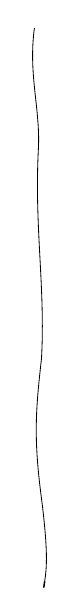
\begin{tikzpicture}[x=1cm,y=1cm,line cap=round]
\draw[line width=.30pt] (.03,0) .. controls (-.05,-.60) and (.11,-1.03) .. (.08,-1.55)
 .. controls (.03,-2.54) and (.17,-3.30) .. (.12,-4.20)
 .. controls (.04,-4.90) and (.02,-5.24) .. (.13,-6.05)
 .. controls (.20,-6.64) and (.19,-6.84) .. (.16,-7.03);
\draw[line width=.55pt] (.16,-7.03) -- (.15,-7.10);
\end{tikzpicture}}}
\unsure{Ainsi}; la donnée de $u_0$
\deleted{\unsure{satisfaisant à}} \inserted{\unsure{autom. ext.}}
à lacets de $\widehat{\Pi}_{0,3}$ \unsure{commutant} à
$\mathfrak S_3$, ou encore
\unsure{un|$u$} autom. ext. de $\widehat{\mathfrak S}_{0,3}^{+}$
\unsure{induisant} l'identité dans $\mathfrak S_3$
et \deleted{\unsure{transformant}}
\inserted{\unsure{laissant invariant}} la classe de conjugaison
du sous-groupe lacet
$L'_0=\varepsilon_0^{\widehat{\mathbb Z}}={\ell'_0}^{\widehat{\mathbb Z}}
=\widehat{\varphi}(L_0)$,
ou encore celle d'un autom. à lacets
$u_0$ de $\widehat{\Pi}_{0,3}$ \unsure{commutant} à
$\sigma_\infty$, et \unsure{ext.\textsuperscript{t}} à $\rho$,
ou encore d'un autom. $u$ de $\widehat{\mathfrak S}_{0,3}^{+}$
qui fixe $\sigma_\infty$, et qui fixe $\rho$ mod $\widehat{\Pi}_{0,3}$
--- \unsure{équivaut à} la donnée de $g_0\in\widehat{\Pi}_{0,3}$ mod $L_0$,
et de $\gamma\in\widehat{\mathbb Z}$, satisfaisant la relation
\scanpage{73}
\mspage{325}

\margin{\figure{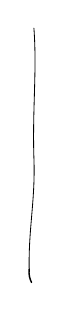
\begin{tikzpicture}[x=1cm,y=1cm,line cap=round]
\draw[line width=.30pt] (.04,0) .. controls (.08,-.55) and (.02,-1.02) .. (.04,-1.65)
 .. controls (.06,-2.18) and (-.03,-2.54) .. (-.02,-3.06);
\draw[line width=.52pt] (-.02,-3.06) .. controls (-.03,-3.13) and (-.01,-3.19) .. (.01,-3.23);
\end{tikzpicture}}}
\[
(38)\qquad \uline{g\rho(g)\rho^2(g)=1},
\]
où $g$ est donné par (40), et où $u$ s'exprime en termes de
\deleted{$g$} $g$ donc de $g_0,\gamma$ par
\[
(36)\qquad
\left\{\begin{aligned}
u(\sigma_\infty)&=\sigma_\infty\\
u(\rho)&=g\rho\qquad
\left(=\underbrace{\sigma_\infty(g_0)\ell_1^\gamma\rho(g_0)^{-1}}_g\rho\right).
\end{aligned}\right.
\]

\deleted{La relation (42)\inserted{\unsure{cf = ci-dessus}}, s'écrit alors,
comme $L_0$ est engendré par}
\[
\deleted{\ell_0=\underbrace{\ell'_0}_{\varepsilon_0}^{2}=(\sigma_\infty\rho)^2\deleted{\unsure{\sigma_\infty}}=\sigma_\infty\rho\sigma_\infty\rho}
\]
\[
\deleted{\underbrace{(u(\sigma_\infty\rho))}_{
\substack{\sigma_\infty g\rho=g_0\sigma_\infty \ell_1^\gamma\rho g_0^{-1}
=\operatorname{int}(g_0)(\sigma_\infty \ell_1^\gamma\rho)}}^{\unsure{2|4}}
\in\operatorname{int}(g_0)(\unsure{L'_0|L_0})\qquad\text{\unsure{or}}}
\]
\[
\deleted{\operatorname{int}(g_0)(\sigma_\infty \ell_1^\gamma\rho)^2\deleted{\unsure{g_0^{-1}}=1}}
\]
\deleted{donc (42) s'écrit}
\[
\deleted{(\sigma_\infty \ell_1^\gamma\rho)^2\in L_0}
\]
\deleted{\unsure{soit}}
\[
\deleted{
\underbrace{\sigma_\infty \ell_1^\gamma\sigma_\infty}_{
    \underbrace{\sigma_\infty(\ell_1)}_{\ell_0}^{\gamma}}
  \underbrace{\sigma_\infty\illegible{1}\rho}_{\varepsilon_0}
}
\]
\margin{\deleted{NB $\operatorname{int}(g_0^{-1})u(\ell_0)$}}
\margin{\deleted{NB on a
$(\operatorname{int}(g_0^{-1})u)(\ell_0)
=(\sigma_\infty \ell_1^\gamma\rho)^2=\ell_0^{2\gamma+1}$}}
\deleted{\unsure{soit}}
\[
\deleted{\overset{\varepsilon_0^{2\gamma+1}}{\unsure{\ell_0^\gamma}\ \underbrace{\varepsilon_0}_{\unsure{\varepsilon_0^{2\gamma}}}}\in L_0}
\]
\deleted{donc \unsure{\ldots}}
\[
\deleted{\unsure{\operatorname{int}(g_0)}\quad u(\ell_0)=}
\]

La relation (42), ou la relation \unsure{en apparence} plus forte
\[
(43)\qquad u(L'_0)\subset\operatorname{int}(g_0)(L'_0)
\]
s'écrit
\[
\underbrace{\operatorname{int}(g_0^{-1})\,
\underbrace{u(\underbrace{\sigma_\infty\rho}_{\ell'_0=\varepsilon_0})}_{
\sigma_\infty g\rho=g_0\sigma_\infty \ell_1^\gamma\rho g_0^{-1}}}_{
\sigma_\infty \ell_1^\gamma\rho
=\underbrace{\underbrace{\sigma_\infty \ell_1^\gamma\sigma_\infty}_{
 \underbrace{\sigma_\infty(\ell_1)^\gamma}_{\ell_0^\gamma=\varepsilon_0^{2\gamma}}}
\underbrace{\sigma_\infty\rho}_{\deleted{\unsure{\sigma_\infty\rho}}\varepsilon_0}}_{
\varepsilon_0^{2\gamma+1}}}
\in L'_0
\]
\margin{\uline{NB} on a
$\operatorname{int}(g_0^{-1})u(\underbrace{\ell'_0}_{\varepsilon_0})
=\varepsilon_0^{2\gamma+1}$}
\unsure{est vérifiée} automatiquement, on \unsure{aura}
$\overline{\mathrm m}$
\[
\deleted{(44)\qquad u(\ell'_0)=u(\varepsilon_0)
=\operatorname{int}(g_0)(\ell'}
\]
\scanpage{74}

\[
(44)\qquad
u\bigl(\underset{\substack{\Vert\\ \varepsilon_0}}{\ell'_0}\bigr)
 = \operatorname{int}(g_0)\bigl(\underset{\substack{\Vert\\ \varepsilon_0}}{\ell'_0}{}^{p}\bigr)
\qquad \text{avec}\quad \uuline{p=2\gamma+1}
\]
d'où (39), \deleted{d'où} en \unsure{élevant} au carré :
\[
u(\ell_0)=\operatorname{int}(g_0)(\ell_0^p).
\]

\deleted{\unsure{On}}\quad
\uline{NB} On \unsure{notera} que si $p\in\widehat{\mathbb Z}^{*}$, alors
$p-1\in 2\widehat{\mathbb Z}$ i.e.\ $\frac{p-1}{2}\in\widehat{\mathbb Z}$,
car il suffit de vérifier la relation analogue pour un $p\in\mathbb Z_\ell^{*}$,
\unsure{pour|que} $p-1\in 2\mathbb Z_\ell$, or si $\ell\ne2$ on a
$2\mathbb Z_\ell=\mathbb Z_\ell$ OK, \unsure{reste} le cas $\ell=2$
$p\in\mathbb Z_2^{*}$ donc l'image de $p$ dans $\mathbb Z/4\mathbb Z$
est $1$ ou $3$ donc $p-1\equiv0$ ou $2\bmod4$
\deleted{\illegible{3}} donc $\frac{p-1}{2}\in\mathbb Z_2$, OK.

\deleted{\unsure{Il reste donc à expri}}\par
Il reste donc à \unsure{exprimer} la condition (38), et on l'écrit
\deleted{\unsure{sous la forme}}
\[
\underbrace{\sigma_\infty(g_0)\ell_1^\gamma\rho(g_0^{-1})}\,
\underbrace{\rho\sigma_\infty(g_0)\ell_\infty^\gamma\rho^2(g_0^{-1})}\,
\rho^2\sigma_\infty(g_0)\ell_0^\gamma g_0^{-1}=1
\]
soit, en appliquant $\operatorname{int}(g_0^{-1})$ et
\deleted{\illegible{2}}\inserted{\unsure{posant encore}}
(cf (8))
\[
(45)\qquad g_0^{-1}\sigma_\infty(g_0)=h_0^{-1}
\qquad\text{i.e.}\quad
h_0=\sigma_\infty(g_0)^{-1}g_0=[\sigma_\infty,g_0^{-1}]
\]
\[
h_0^{-1}\ell_1^\gamma\underbrace{\rho(h_0^{-1})\ell_\infty^\gamma}\,
\rho^2(h_0^{-1})\ell_0^\gamma=1
\]
ou encore, en appliquant $\operatorname{int}(\ell_0^\gamma)$
\[
(46)\qquad
\boxed{\underbrace{(\ell_0^\gamma h_0^{-1})}\cdot
\rho(\ell_0^\gamma h_0^{-1})\cdot\rho^2(\ell_0^\gamma h_0^{-1})=1}
\qquad\left(\text{où }\gamma=\frac{p-1}{2}\right)
\]
ce qui n'est autre que (10). Quant à la condition \unsure{(9)|(7)},
on voit qu'elle est \inserted{superflue, i.e.,} automatiquement vérifiée.
\scanpage{75}
\mspage{326}

Résumons :

\uline{Théorème} Un autom. ext.\ \inserted{\unsure{à lcts|à lacets}} de
$\widehat{\Pi}_{0,3}$ commutant à
$\mathfrak S_3$, se relève de façon unique comme autom.
du groupe \unsure{à lcts|à lacets} $\widehat{\Pi}_{0,3}$, commutant à
$\sigma_\infty$ (et commutant à $\rho$ mod autom.\ \unsure{intérieures|intérieurs}),
ou encore comme restriction d'un autom.\ $u$ de
$\widehat{\mathfrak S}_{0,3}^{+}$
qui fixe $\sigma_\infty$, \unsure{invarie} $\rho$ mod $\widehat{\Pi}_{0,3}$
(i.e.\ \inserted{fixe} $\dot\rho$ dans $\mathfrak S_3$),
et qui \unsure{invarie} la classe de conjugaison du s-groupe
\inserted{fermé} $L'_0$\inserted{$=\widehat\varphi(L_0)$}
\deleted{\illegible{3}} engendré par $\ell'_0=\varepsilon_0=\sigma_\infty\rho$.
(ou encore du sous-groupe \inserted{fermé} $L_0=(L'_0)^2$ engendré par $\ell_0$).
La donnée d'un tel $u$ équivaut à celle de son multiplicateur
$p\in\widehat{\mathbb Z}^{*}$, et d'un $g_0\in\widehat{\Pi}_{0,3}/L_0$
satisfaisant les conditions suivantes

 a) Posant
\[
(47)\qquad
\begin{cases}
h_0=\sigma_\infty(g_0)^{-1}g_0=[\sigma_\infty,g_0^{-1}]
   \quad(\in\widehat{\Pi}_{0,3})\\
\gamma=\dfrac{p-1}{2}\in\widehat{\mathbb Z}
\end{cases}
\]
on a la relation (46) ci-dessus (invariante par remplacement de $g_0$ par
$g_0\ell_0^\lambda$, $\lambda\in\widehat{\mathbb Z}$)
\[
(48)\qquad
\bigl(\underbrace{\ell_0^\gamma h_0^{-1}}_{\xi_0}\bigr)
\rho(\ell_0^\gamma h_0^{-1})\rho^2(\ell_0^\gamma h_0^{-1})=1
\]
\margin{i.e.\ $\xi_0\rho(\xi_0)
\rho^{\unsure{2}}(\xi_0)=1$ avec
$\xi_0=\ell_0^\gamma h_0^{-1}$}

 b) $\sigma_\infty$ et $g\rho$ engendrent \unsure{top.}
$\widehat{\mathfrak S}_{0,3}^{+}$,
où $g$ est donné en fonction de $g_0$ par 40
\[
[(40)]\qquad
g=\sigma_\infty(g_0)\ell_1^\gamma\rho(g_0)^{-1}
=\sigma_\infty(g_0\ell_0^\gamma)\rho(g_0^{-1})
\]
\margin{$\begin{aligned}
&=g_0(h_0^{-1}\ell_1^\gamma)\rho(g_0)^{-1}\\
&=(g_0\ell_0^{-\gamma})(\ell_0^\gamma h_0^{-1})
  (\rho(g_0\ell_0^{-\gamma}))^{-1}
\end{aligned}$}

\deleted{\illegible{3}}
(\uline{NB} la relation (46) équivaut à :
\inserted{$(g\rho)^3=1$ i.e.\ à}
\[
(38)\qquad g\rho(g)\rho^2(g)=1,
\]
exprimée directement en termes de $g_0$, $\gamma=\frac{p-1}{2}$),
avec les relations génératrices $\sigma_\infty^2=(g\rho)^3=1$.
\margin{(36)}L'autom.\ $u$ est donné en termes de $g_0$ et de $p$ par
\scanpage{76}

\[
[(36)]\qquad
\begin{cases}
u(\sigma_\infty)=\sigma_\infty\\
u(\rho)=g\rho
\end{cases}
\qquad\text{où }g\text{ donné par }[(40)])
\]

On aura alors
\[
(49)\qquad
\begin{cases}
u(\ell_0)=\operatorname{int}(g_0)\ell_0^p\\
u(\ell_1)=\operatorname{int}(g_1)\ell_1^p
 \inserted{{}=\operatorname{int}(\sigma_\infty(g_0))(\ell_1^p)}\\
u(\ell_\infty)=\operatorname{int}(g_\infty)(\ell_\infty^p)
\end{cases}
\]
\margin{$\begin{aligned}
g_1&=g\rho(g_0)=\sigma_\infty(g_0)\ell_1^\gamma\\
   &=\sigma_\infty(g_0\ell_0^\gamma)\\
g_\infty&=g\rho(g_1)=\deleted{\unsure{g}}g\rho(g)\rho^2(g_0)\\
   &=\rho^2(g^{-1}g_0)=\rho(g_0\ell_0^\gamma)h_0
\end{aligned}$}

\margin{cf \unsure{prop.} plus haut}
\deleted{
\uline{Corollaire} Pour que l'hom.\ \unsure{surj.} (18)
\[
\widehat\varphi:\widehat\Pi_{\unsure{0,3|3}}
\longrightarrow
\widehat{\mathfrak S}_{0,3}^{+}
\]
\deleted{\unsure{déf}} défini par
\[
\ell_0\longmapsto \ell'_0=\sigma_\infty\rho,\quad
\ell_1\longmapsto \ell'_1=\sigma_\infty,\quad
\ell_\infty\longmapsto \ell'_\infty=\rho^{-1},
\]
commute \inserted{extérieurement} à $u$, il f. et s.\ qu'on puisse
\unsure{trouver} $\beta\in\widehat{\mathbb Z}$ tel qu'on ait
\[
[(24)]\qquad
\varepsilon_1^{-\beta}h_0\varepsilon_0^\beta
=\sigma_\infty(\widehat\varphi(h_0))^{-1}\widehat\varphi(h_0)
\]
ou ce qui revient au $\overline{\mathrm m}$, qu'il existe
$\alpha\in\widehat{\mathbb Z}$ tel qu'on ait
\[
[(\unsure{30|38})]\qquad
\deleted{\unsure{h_0^{-1}}\ell_1^\gamma\rho
=\operatorname{int}(\varepsilon_0^\alpha\widehat\varphi(
\unsure{\rho^{-1}(h_0)|\rho^{-1}h_0)}))(\rho^p)}
\]
\deleted{$u(\rho)=\operatorname{int}($}
\[
h_0^{-1}\ell_1^\gamma\rho
=\operatorname{int}(\varepsilon_0^\alpha\widehat\varphi(
\unsure{\rho^{-1}(h_0)|\rho^{-1}h_0)}))(\rho^p)
\]
(où nécessairement $\alpha=\beta+\gamma$).
}
\margin{$\beta$ \unsure{resp.} $\alpha$ sont \unsure{uniquement} \unsure{déterminés}}
\scanpage{77}
\mspage{327}

\uline{\unsure{Scholie}} Dans le \unsure{th.}, \unsure{le} $g$ \inserted{$\in\widehat{\Pi}_{0,3}$} (qui \unsure{intervient} directement pour écrire $u$) s'exprime par l'intermédiaire du $g_0$ \inserted{$\in\widehat{\Pi}_{0,3}$} et $\gamma=\frac{p-1}{2}$, \deleted{\illegible{2}} ($g_0$ défini mod $L_0$) --- la condition (46) étant en fait une condition qui s'exprime directement en termes de $g_0$, ou mieux encore, en termes de
\[
(50)\qquad
\xi_{\unsure{\deleted{0}|0}}=\ell_0^\gamma h_0^{-1}\in\widehat{\Pi}_{0,3}
\quad\text{(d'où }h_0=\xi_{\unsure{\deleted{0}|0}}^{-1}\ell_0^\gamma\text{)}
\]
comme
\[
(\unsure{51})\qquad \xi\rho(\xi)\rho^2(\xi)=1,
\]
qui équivaut à
\[
(52)\qquad (\xi\rho)^3=1.
\]

Les solutions de l'équation (\unsure{51}), ou ce qui revient au $\overline{\mathrm m}$ de (52), \unsure{correspondent} aux scindages de \unsure{la|l'}\inserted{\unsure{sous-}}extension \inserted{de $\widehat{\mathfrak S}_{0,3}^{+}$} de $\mathbb Z/3\mathbb Z$ par $\widehat{\Pi}_{0,3}$, \unsure{engendrée} par $\rho\in\mathfrak S_3$, \deleted{\illegible{1}} i.e. aux éléments d'ordre 3 de $\widehat{\mathfrak S}_{0,3}^{+}$ au dessus de $\dot\rho$.
Sur l'ens de ces scindages resp. de ces éléments $\xi\rho$, $\widehat{\Pi}_{0,3}$ opère par autom. intérieurs :
\[
(53)\qquad
\mathrm{int}(\lambda)(\xi\rho)
=\lambda\xi\rho\lambda^{-1}
=\lambda\xi\rho\lambda^{-1}\rho^{-1}\rho
=(\lambda\xi\rho(\lambda)^{-1})\rho
\]
i.e. il opère sur l'ens des solutions de (\unsure{51}), par
\[
(54)\qquad {}^\lambda\xi=\lambda\xi\rho(\lambda)^{-1}
\]
\margin{\uline{NB} $\lambda\mapsto{}^\lambda\xi$ est injectif}
\scanpage{78}

Admettons (quitte à le vérifier par la suite) qu'il y a exactement \unsure{deux} classes de conjugaison : celle de $\xi_0=1$, correspondant au scindage tautologique, \deleted{\illegible{1}}\inserted{de} sorte que pour de tels $\xi$ on aura
\[
(55)\qquad \xi=\lambda\rho(\lambda)^{-1}
\qquad(\lambda\in\widehat{\Pi}_{0,3}),
\]
et d'autre part la classe de conjugaison du \unsure{rel$^{\mathrm t}$} d'ordre 3 $\sigma_\infty\rho^{-1}\sigma_\infty^{-1}=\sigma_\infty\rho^{-1}\sigma_\infty$ de $\dot\rho$, correspondant à
\[
\sigma_\infty\rho^{-1}\sigma_\infty=\xi_0\rho,\quad\text{avec}
\]
\[
\left\{\begin{aligned}
\xi_0&=\sigma_\infty\rho^{-1}\sigma_\infty\rho^{-1}
=\sigma_\infty\underbrace{(\rho^{-1}\sigma_\infty)}_{\varepsilon_0^{-1}}(\rho^{-1}\sigma_\infty)\sigma_\infty\\
&=\sigma_\infty\varepsilon_0^{-2}\deleted{\unsure{=}}\sigma_\infty
=\sigma_\infty(\ell_0^{-1})=\ell_1^{-1}
\end{aligned}\right.
\]
(et on a bien
\[
\ell_1^{-1}\rho(\ell_1^{-1})\rho^2(\ell_1^{-1})
=\ell_1^{-1}\ell_\infty^{-1}\ell_0^{-1}
=(\ell_0\ell_\infty\ell_1)^{-1}=1
\]
), Cette orbite correspond à des solutions de la forme \deleted{\illegible{1}}
\[
(56)\qquad \xi=\lambda\ell_0^{-1}\rho(\lambda)^{-1}
\qquad(\lambda\in\widehat{\Pi}_{0,3})
\]
[on \unsure{notera} que $\ell_0^{-1}$ et $\ell_1^{-1}$ sont sur la $\overline{\mathrm m}$ orbite
\[
\ell_1^{-1}=\deleted{\unsure{\ell_0\ell_1}\ \lambda\ell_1^{-1}\rho(\lambda)^{-1}}
\ell_0(\ell_0^{-1})\rho(\ell_0)^{-1}
\]
]

i.e. \deleted{$\ell_0=\rho(\lambda)\ell_1\lambda^{-1}$ \illegible{1} où $\lambda=\ell_\infty\ell_{\unsure{0}}$}

\deleted{Posons}
\deleted{\unsure{a)}}

A) Cas \deleted{\unsure{A}} où $\xi$ est de la forme (55), donc
\[
(\unsure{56|57})\qquad h_0=\rho(\lambda)\lambda^{-1}\ell_0^\gamma
\]
\scanpage{79}
\mspage{328}

Il reste donc à résoudre l'équation en $g_0$ (47)
\[
(58)\qquad
\sigma_\infty(g_0)^{-1}g_0
=\underbrace{\rho(\lambda)\lambda^{-1}\ell_0^\gamma}_{h_0}
\]
Pour \unsure{$\forall$|un} $h_0$ fixé, il y a au plus un seul $g_0$ qui satisfait à cette condition, et un tel $g_0$ existe \unsure{ssi} \deleted{$\sigma_\infty(h_0)h_0=1$}, ce qui s'écrit
\margin{\unsure{en utilisant} \unsure{que} $\widehat{\Pi}_{0,3}^{\sigma_\infty}=\{1\}$}
\[
(59)\qquad \sigma_\infty(h_0)\cdot h_0=1
\qquad\inserted{\text{ou encore }h_0\sigma_\infty(h_0)=1}
\]
\deleted{$\sigma_\infty(\rho(\lambda))\sigma_\infty(\lambda^{-1})\ell_1^\gamma\rho(\lambda)\lambda^{-1}\ell_0^\gamma=1$}

qui s'écrit aussi, en reprenant l'expression $h_0=\xi^{-1}\ell_0^\gamma$
\[
\deleted{(\unsure{60})}\qquad
\sigma_\infty(\xi)^{-1}\ell_1^\gamma\xi^{-1}\ell_0^\gamma=1
\qquad\text{i.e.}
\]
\[
(60)\qquad \sigma_\infty(\xi)=\ell_1^\gamma\cdot\xi^{-1}\cdot\ell_0^\gamma
\]

En résumé

\uline{Corollaire} Les $u$ qui ne changent pas la classe de \inserted{$\widehat{\Pi}_{0,3}$-}conjugaison de $\rho$ \deleted{sont} correspondent 1-1 aux systèmes $(\lambda,p)\in L_0\backslash\widehat{\Pi}_{0,3}\times\widehat{\mathbb Z}^{*}$, tels que --- posant $\xi=\lambda\rho(\lambda)^{-1}$, \inserted{$\gamma=\frac{p-1}{2}$,} on ait la relation (60).
On notera que pour $\lambda$ \unsure{donc} $\xi$ fixé, il existe au plus \uuline{un} $\gamma\in\widehat{\mathbb Z}$ tel que la relation (60) soit valable, donc $p$ est déterminé par $\lambda$, soumis à la condition \unsure{suppl.} que \inserted{l'élément} $2\gamma+1$ de $\widehat{\mathbb Z}$ soit dans $\widehat{\mathbb Z}^{*}$ (i.e. $\exists\gamma'\in\widehat{\mathbb Z}^{*}$ \unsure{avec} $2\gamma\gamma'+\gamma+\gamma'=0$)
\scanpage{80}

\uline{NB} Si $\lambda$ est remplacé par $\lambda'=\ell_0^\alpha\lambda$, $\xi=\lambda\rho(\lambda)^{-1}$ est remplacé par $\xi'=\ell_0^\alpha\cdot\xi\rho(\ell_0)^{-\alpha}$, et $h_0=\xi^{-1}\ell_0^\gamma$ est remplacé par $h'_0=\rho(\ell_0)^\alpha h_0\ell_0^{-\alpha}$, enfin $g_0$ est remplacé par $g'_0=g_0\ell_0^{-\alpha}$, OK. \unsure{!} (L'équation (60) pour $\xi$ \unsure{ou} pour $\xi'$ est équivalente)

Finalement, que $u$ change ou ne change pas la classe de $\widehat{\Pi}_{0,3}$-conj. de $\rho$, la démarche la plus claire pour déterminer les $u$ en question me semble celle-ci :

1$^\circ$) On choisit un $\xi$ \inserted{$\in\widehat{\Pi}_{0,3}$} satisfaisant l'équation
\[
(A)\qquad \xi\rho(\xi)\rho^2(\xi)=1
\]
(on le \unsure{prendra} soit sous la forme (55), soit sous la forme (56)\deleted{\unsure{)}} :
\[
(B)\qquad
\xi=\lambda\rho(\lambda)^{-1}
\quad\text{ou}\quad
\xi=\lambda\ell_0^{-1}\rho(\lambda)^{-1}
\quad\deleted{\unsure{\rbrace|\xi}},\quad\text{avec }\lambda\in\widehat{\Pi}_{0,3}
\]
)

2$^\circ$) On choisit $\gamma\in\widehat{\mathbb Z}$ tel que
\[
(C)\qquad \sigma_\infty(\xi)=\ell_1^\gamma\xi^{-1}\ell_0^\gamma
\]
\margin{ici, $\xi$ est \unsure{donc} donné en termes de $\lambda$ \unsure{par par|par} (B)}
ce qui détermine $\gamma$ de façon unique. On devra dans \unsure{1$^\circ$)|2$^\circ$)} se borner aux $\xi$ \inserted{(i.e. aux $\lambda$)} pour lesquels un tel $\gamma$ existe, et tel de plus que $p=2\gamma+1$ soit $\in\widehat{\mathbb Z}^{*}$.
% ===== LM_P067: second pass, checked against the scans =====
\scanpage{81}
\mspage{329}

$3^\circ)$ On construit alors
\[
h_0=\xi^{-1}\ell_0^{\gamma}
\in\widehat{\Pi}_{0,3}
\]
La relation du $2^\circ)$ assure que $h_0\sigma_\infty(h_0)=1$ i.e.
que $h_0$ peut se mettre sous la forme
\[
h_0=\sigma_\infty(g_0)^{-1}g_0
\]
\unsure{avec} $g_0\in\widehat{\Pi}_{0,3}$.

\margin{NB Il faudrait s'assurer par contre que la connaissance de $g_0$
\unsure{ne} détermine pas $\gamma$ i.e. $p$
i.e. que \deleted{\illegible{2}} le $\gamma$
tel que $\xi=\ell_0^{\gamma}h_0^{-1}$
\unsure{satisfasse} (A) \unsure{ne} soit pas \deleted{\illegible{1}} unique.
À éclaircir!}

$4^\circ)$ On peut maintenant poser
\[
g=\sigma_\infty(g_0)\ell_1^{\gamma}\rho(g_0)^{-1}
=(g_0\ell_0^{-\gamma})\xi
\rho(g_0\ell_0^{-\gamma})^{-1}
\]
et on \deleted{\unsure{définit}} a ce qu'il faut pour définir $u$, via
\[
\left\{
\begin{aligned}
u(\sigma_\infty)&=\sigma_\infty\\
u(\rho)&=g\rho
\end{aligned}
\right.
\]

Ici, la seule équation délicate, \deleted{pour} laquelle
l'existence (non l'unicité, en bon cas) d'une solution, est problématique,
est l'équation C (en $\gamma\in\widehat{\mathbb Z}$)
--- plus la condition encore que $2\gamma+1\in\widehat{\mathbb Z}^{*}$.
C'est donc une \deleted{\unsure{question}}\inserted{\uline{condition}}
sur $\lambda\in\widehat{\Pi}_{0,3}$ --- ou plutôt deux types de condition,
suivant que $\xi$ est défini en termes de $\lambda$ par
l'une ou l'autre formule (B).

Je prévois qu'on est dans l'une ou

\margin{80}
\scanpage{82}

l'autre cas des formules (B), suivant que $p\bmod 3$ est congru à $1$, ou à $-1$
(NB. il ne doit pas être congru à $0$, puisque $p\bmod 3\in(\mathbb Z/3\mathbb Z)^*$)
i.e. suivant que $2\gamma\equiv 0$ ou $-2$ $(3)$ i.e.
$\gamma\equiv 0$ ou $-1$ $(3)$
(NB. il ne faut pas que $\gamma$ soit $\equiv 1$ $(3)$,
sinon $2\gamma+1=p$ serait congru à $0\bmod(3)$).
C'est en tous cas ce qui \unsure{sera} le cas si $u\in\Gamma_{\mathbb Q_0}$.

Pour le tester, réduisons le \deleted{\illegible{1}}\inserted{groupe}
$\widehat{\mathfrak S}_{0,3}^{+}$
mod l\deleted{es}\inserted{'}\unsure{équation|équations}
$\ell_0^3=1$ i.e. $(\sigma_\infty\rho)^6=1$
\[
\deleted{\ell_0^3=\ell_1^3=\ell_\infty^3=1\quad\ell_\infty}
\]
de sorte que $\widehat{\mathfrak S}_{0,3}^{+}$
est \unsure{remplacé} par une extension de $\mathfrak S_3$
par le groupe défini par les générateurs $\ell_0,\ell_1,\ell_\infty$ satisfaisant
\[
\unsure{\ell_0}^3=\ell_1^3=\ell_\infty^3=(\ell_\infty\ell_1\ell_0)=1
\]
--- ou mieux, utilisons
\[
\widehat{\mathfrak S}_{0,3}^{+}
\simeq\mathrm{Sl}(2,\mathbb Z)^{\prime\,\wedge}
\]
et réduisons carrément dans
\[
\mathrm{Sl}(2,\mathbb Z/6\mathbb Z)'
\simeq\mathrm{Sl}(2,\mathbb Z/2\mathbb Z)
\times\mathrm{Sl}(2,\mathbb Z/3\mathbb Z)'.
\]

\margin{81}
\scanpage{83}
\mspage{330}

Mais pour faire les calculs, il faut pouvoir identifier $\sigma_\infty$
\inserted{et} $\rho$ comme éléments de
$\mathrm{Sl}(2,\unsure{\widehat{\mathbb Z}|\mathbb Z})$
--- explicitation que nous ferons tantôt.

\begin{center}\rule{2cm}{0.4pt}\end{center}

Revenant à (24 bis), et y portant
$\unsure{h_0|h_\infty}=\xi^{-1}\ell_0^{\gamma}$, il vient
\[
\tag{61}
g_0=\widehat{\varphi}(\xi)
\varepsilon_0^{\gamma-\beta}
\]
On pense donc que $u$ correspond à
$(\xi,g_0,\gamma,\beta)$,
avec $\xi,g_0\in\widehat{\Pi}_{0,3}$
et $\gamma,\beta\in\widehat{\mathbb Z}$
\margin{\illegible{1}}
satisfaisant
\[
\tag{62}
\left\{
\begin{aligned}
&\xi\rho(\xi)\rho^2(\xi)=1\\
&\xi\underbrace{\sigma_\infty(g_0)^{-1}g_0}_{h}
=\ell_0^{\gamma}\\
&\deleted{\unsure{\widehat{\varphi}(\xi)}}g_0
=\widehat{\varphi}(\xi)
\varepsilon_0^{\gamma-\beta}\\
&2\gamma+1\in\widehat{\mathbb Z}^{*}
\end{aligned}
\right.
\]
dont on peut éliminer $g_0$, et on trouve des équations en
$(\xi,\deleted{\gamma}r,\deleted{\beta}s)$
$(r=\gamma-\beta,\ s=\gamma+\beta)$
\[
\tag{63}
\left\{
\begin{aligned}
&\xi\rho(\xi)\rho^2(\xi)=1\\
&\sigma_\infty\bigl(\widehat{\varphi}(\xi)\bigr)^{-1}
\widehat{\varphi}(\xi)
=\varepsilon_1^r\xi^{-1}\varepsilon_0^s\\
&\underbrace{r+s+1}_{p}\in\widehat{\mathbb Z}^{*}
\end{aligned}
\right.
\]
\margin{(donc $\xi=\lambda\rho(\lambda)^{-1}$
ou $\xi=\lambda\ell_0^{-1}\rho(\lambda)^{-1}$}

Ici, $\unsure{\lambda}$ est déterminé mod transformation en
$\lambda'=\deleted{\unsure{\ell_0^{\alpha}\xi}}\ell_0^\alpha\lambda$
donc $\xi$ devient
$\xi'=\ell_0^\alpha\xi\ell_1^{-\alpha}$

\margin{82}
\scanpage{84}
\mspage{331}

\uline{42} Récapitulation sur le groupe
\[
(\mathfrak S_{0,3})
\simeq
\bigl(\Pi_1(U_{0,3}^{\mathrm{an}},\mathfrak S_3;-\bar j)\bigr)
\simeq
\bigl(\widetilde\Pi'_{0,3}\simeq
\Pi_1((\mathbb P^{1\mathrm{an}},0\{0\}+2\{1\}+3\{\infty\}),\unsure{\{1,\tau\}};-\bar j)\bigr)
\]
\[
\simeq\bigl(\mathrm{Gl}(2,\mathbb Z)'=\mathrm{Gl}(2,\mathbb Z)/\{\pm1\}
\simeq\mathrm{GP}(1,\mathbb Z)\bigr)
\simeq\bigl(\mathcal T'_{1,1}=\mathcal T_{1,1}/\{\pm1\}\bigr)
\]
et sur les automorphismes ``de lacets'' de
$\widehat{\mathfrak S}_{0,3}^{+}$ et de
$\widehat\Pi_{0,3}$ (Formulaire fondamental).

\margin{\deleted{\illegible{1}} $\mathfrak S_{0,3}$ défini comme $\mathrm{Aut}_{\mathrm{lac}}(\Pi_{0,3})$ --- on en donne \uline{cinq} \unsure{visions} différentes ! (En fait, il y en a \uline{une} dizaine, cf. (V) ci-dessous\ldots)}

\uline{I}) $\mathcal T_{0,3}$

Le groupe $\mathfrak S_{0,3}$ est \unsure{présenté} comme une extension
\[
(1)\qquad
\diagram{\begin{tikzcd}[ampersand replacement=\&,column sep=small]
1 \arrow[r,dash] \& \Pi_{0,3} \arrow[r] \arrow[d,phantom,"\Vert"] \& \mathfrak S_{0,3} \arrow[r] \& \mathcal T_{0,3} \arrow[r] \arrow[d,phantom,"\wr"] \& 1 \\
\& \Pi_1(U_{0,3}^{\mathrm{an}};-\bar j) \&\& \mathfrak S_3\times\mathbb Z/2\mathbb Z \&
\end{tikzcd}}
\]
où $\mathfrak S_3\times\mathbb Z/2\mathbb Z$ est considéré comme groupe opérant sur
$U_{0,3}^{\mathrm{an}}=\mathbb P^{1\mathrm{an}}\setminus\{0,1,\infty\}=\mathbb C\setminus\{0,1\}$,
\deleted{par \unsure{autom.} holomorphes}
\deleted{$\mathfrak S_3$ opérant par permutations}
--- c'est le groupe des automorphismes conformes \unsure{du|de} $\mathbb P^{1\mathrm{an}}$ qui stabilisent $\{0,1,\infty\}$.
Le groupe \margin{\unsure{(2)}}\deleted{\unsure{$\mathfrak S_3$}}\inserted{$\mathfrak S_3=\mathfrak S_{\{0,1,\infty\}}$} est le sous-groupe des \deleted{\unsure{éléments}}automorphismes conformes, il s'identifie au groupe des permutations de $\{0,1,\infty\}$, ses six éléments sont
\unsure{$\mathrm{id}$;|$1$;}
$\dot\sigma_0,\dot\sigma_1,\dot\sigma_\infty$ (\inserted{les trois} transpositions),
$\dot\rho,\deleted{\unsure{\dot{\rho}}}\dot\rho^{-1}$ (permutations circulaires)
donnés par les formules explicites
\[
(2)\qquad
\left\{\begin{array}{l}
\dot\sigma_0(z)=\dfrac{z}{z-1}\inserted{\unsure{=1+\dfrac{1}{1-z}|=1+\dfrac{1}{z-1}}},\quad
\dot\sigma_1(z)=\dfrac1z,\quad
\dot\sigma_\infty(z)=1-z,\\[4pt]
\dot\rho(z)=\dfrac1{1-z},\quad
\dot\rho^{-1}(z)=1-\dfrac1z=\dfrac{z-1}{z},
\end{array}\right.
\]
avec
\[
(3)\qquad
\left\{\begin{array}{l}
\dot\sigma_0\dot\sigma_1=\dot\sigma_1\dot\sigma_\infty=\dot\sigma_\infty\dot\sigma_0=\dot\rho,\\
\dot\rho\dot\sigma_0\dot\rho^{-1}=\dot\sigma_1,\quad
\dot\rho\dot\sigma_1\dot\rho^{-1}=\dot\sigma_\infty,\quad
\dot\rho\dot\sigma_\infty\dot\rho^{-1}=\dot\sigma_0
\end{array}\right.
\]
\[
(4)\qquad
\dot\sigma_0^2=\dot\sigma_1^2=\dot\sigma_\infty^2=\dot\rho^3=1.
\]
Le groupe $\mathcal T'_{0,3}=\mathbb Z/2\mathbb Z\subset\mathcal T_{0,3}$ apparaît comme le centre,
\margin{83}
\scanpage{85}

il est engendré par la conjugaison complexe $\tau$
\[
(5)\qquad ,\quad \tau(z)=\bar z,
\]
les cinq autres éléments de $\mathcal T_{0,3}$ sont
\[
\deleted{\unsure{\tau\sigma}}\quad(6)\qquad
\tau\dot\sigma_0=\dot\tau_0,\quad
\tau\dot\sigma_1=\dot\tau_1,\quad
\tau\dot\sigma_\infty=\dot\tau_\infty,\quad
\tau\rho,\quad\tau\rho^{-1}=(\tau\rho)^{-1},
\]
les \unsure{antiinvolutions|anti-involutions} $\tau'_i$ $(i=0,1,\infty)$ sont particulièrement intéressantes, \unsure{données} par
\[
(7)\qquad
\unsure{\dot\tau'_0(z)}=\frac{\bar z}{\bar z-1},\quad
\unsure{\dot\tau'_1(z)}=\frac1{\bar z},\quad
\dot\tau'_\infty(z)=1-\bar z.
\]

Les points fixes \deleted{\unsure{dans $U_{0,3}$}} des \inserted{\illegible{1}} autom. conformes de \deleted{\illegible{2}} $(\mathbb P^{1\mathrm{an}},\{0,1,\infty\})$ sont les suivants
\[
(8)\qquad
\left\{\begin{array}{l}
(\mathbb P^1_{\mathbb C})^{\dot\sigma_0}=\{0,2\},\quad
(\mathbb P^1_{\mathbb C})^{\dot\sigma_1}=\{1,-1\},\quad
(\mathbb P^1_{\mathbb C})^{\dot\sigma_\infty}=\{\infty,\frac12\}\\[3pt]
\mathbb P_{\mathbb C}^{1\,\dot\rho}=\mathbb P^{1\,\dot\rho^{-1}}=\{-\bar j,-j\}
\end{array}\right.
\qquad
\begin{array}{l}
\text{où }j=\exp 2i\pi/3=\dfrac{-1+i\sqrt3}{2}\quad\text{racine primitive}\quad\text{$3^{\unsure{\mathrm{ième}|\mathrm{ème}}}$ de $1$}\\[5pt]
-\bar j=\exp 2i\pi/6=\dfrac{1+i\sqrt3}{2}\quad\text{racine primitive}\quad\text{$6^{\unsure{\mathrm{ième}|\mathrm{ème}}}$ de $1$}
\end{array}
\]

\margin{NB $\mathbb P_{\mathbb C}^{1\,\dot\rho\tau}=\mathbb P_{\mathbb C}^{1\,\dot\rho^{-1}\tau}=\varnothing$}

\[
(9)\qquad
\left\{\begin{array}{l}
\mathbb P_{\mathbb C}^{1\,\tau}=\mathbb P_{\mathbb R}^{1}\\[3pt]
\mathbb P_{\mathbb C}^{1\,\dot\tau'_0}=\{x+iy\mid(x-1)^2+y^2=1\}
\inserted{=\{z\mid z+\bar z=z\bar z\}\unsure{=\frac1z|=\frac12}}
\inserted{\unsure{=\frac12-\mathbb U}},\quad
\mathbb P_{\mathbb C}^{1\,\dot\tau'_1}=\{z\mid z\bar z=1\}=\{x+iy\mid x^2+y^2=1\}=\mathbb U\\[3pt]
\mathbb P_{\mathbb C}^{1\,\dot\tau'_\infty}=\{z\mid z+\bar z=1\}=\{x+iy\mid x=\frac12\}=\frac12+i\mathbb R;
\end{array}\right.
\]

L'image la plus suggestive est sans doute celle de la sphère de Riemann, où $\tau,\dot\tau'_0,\dot\tau'_1,\dot\tau'_\infty$ apparaissent comme les \deleted{\unsure{symétries}}\inserted{\uline{réflexions}} p.r. aux \deleted{``équateurs''}\inserted{``\unsure{gr\textsuperscript{ds}|grands} cercles''} correspondants, qui pour $\tau$ est ``l'équateur'' et pour les autres sont les grands cercles \inserted{``méridiens''}, passant par les pôles $-\bar j,-j$, qui réalisent le découpage de l'équateur en six segments circulaires, par les pts de subdivision $0,\frac12,1,2,\infty,-1$.

\figure{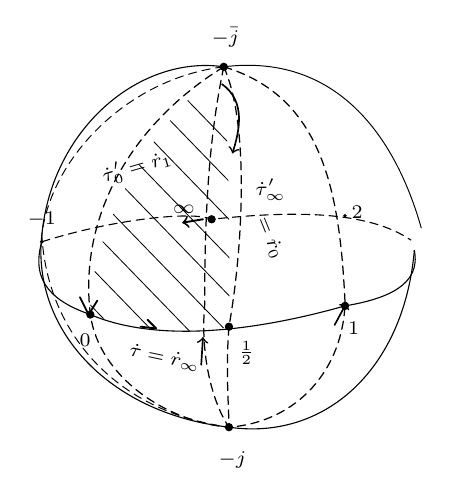
\begin{tikzpicture}[x=.022cm,y=-.022cm,line cap=round,line join=round,font=\scriptsize]
\coordinate (N) at (110,8);
\coordinate (S) at (113,216);
\draw[line width=.4pt] (N) .. controls (62,1) and (11,43) .. (5,105)
 .. controls (-1,158) and (42,208) .. (S)
 .. controls (168,224) and (214,183) .. (220,114);
\draw[line width=.35pt] (N) .. controls (175,0) and (209,48) .. (224,101);
\begin{scope}
\clip (N) .. controls (62,47) and (32,109) .. (33,151)
 .. controls (60,160) and (91,164) .. (113,158)
 .. controls (114,100) and (112,43) .. (N);
\foreach \a in {-80,-58,-36,-14,8,30,52,74,96,118,140,162}
  \draw[line width=.3pt] (-15,\a)--(145,{\a+165});
\end{scope}
\draw[dash pattern=on 3pt off 2pt,line width=.45pt] (N)
 .. controls (58,40) and (26,93) .. (33,151)
 .. controls (38,187) and (77,213) .. (S);
\draw[dash pattern=on 3pt off 2pt,line width=.45pt] (N)
 .. controls (101,51) and (99,95) .. (99,145)
 .. controls (96,180) and (106,206) .. (S);
\draw[dash pattern=on 3pt off 2pt,line width=.45pt] (N)
 .. controls (125,41) and (121,113) .. (113,158)
 .. controls (111,183) and (113,205) .. (S);
\draw[dash pattern=on 3pt off 2pt,line width=.45pt] (N)
 .. controls (167,25) and (177,80) .. (180,144)
 .. controls (179,182) and (153,213) .. (S);
\draw[dash pattern=on 3pt off 2pt,line width=.35pt] (N)
 .. controls (53,15) and (10,62) .. (5,105)
 .. controls (8,161) and (47,207) .. (S);
\draw[dash pattern=on 3pt off 2pt,line width=.4pt] (5,109)
 .. controls (46,96) and (92,91) .. (103,96)
 .. controls (150,91) and (193,91) .. (218,108);
\draw[line width=.4pt] (5,109) .. controls (-2,133) and (13,144) .. (33,151)
 .. controls (80,171) and (148,155) .. (180,146)
 .. controls (204,142) and (224,134) .. (220,114);
\draw[->,line width=.7pt] (98,96)--(86,98);
\draw[->,line width=.6pt] (109,18) .. controls (123,28) and (119,45) .. (115,58);
\draw[->,line width=.6pt] (97,180)--(98,164);
\draw[->,line width=.6pt] (174,157)--(181,144);
\draw[line width=.65pt] (27,141)--(32,151)--(37,143);
\draw[line width=.65pt] (62,158)--(71,159)--(66,154);
\foreach \p in {(110,8),(113,216),(103,96),(33,151),(113,158),(180,146)}
  \fill \p circle[radius=2.4];
\foreach \p in {(5,109),(180,94)}
  \fill \p circle[radius=1.1];
\node[inner sep=0pt] at (111,-9) {$-\bar j$};
\node[inner sep=0pt] at (115,235) {$-j$};
\node[inner sep=0pt] at (5,96) {$-1$};
\node[inner sep=0pt] at (87,90) {$\infty$};
\node[inner sep=0pt] at (187,92) {$2$};
\node[inner sep=0pt] at (30,166) {$0$};
\node[inner sep=0pt] at (123,173) {$\frac12$};
\node[inner sep=0pt] at (185,159) {$1$};
\node[inner sep=0pt,rotate=16] at (60,66) {$\dot\tau'_0=\dot r_1$};
\node[inner sep=0pt] at (137,79) {$\dot\tau'_\infty$};
\node[inner sep=0pt,rotate=-68] at (137,107) {$=\dot r_0$};
\node[inner sep=0pt,rotate=-12] at (76,176) {$\unsure{\dot\tau}=\unsure{\dot r}_\infty$};
\end{tikzpicture}}

Notons aussi les formules
\[
(10)\qquad
\left\{\begin{array}{l}
\dot\rho\dot\tau'_0\dot\rho^{-1}=\dot\tau'_1,\quad
\dot\rho\dot\tau'_1\dot\rho^{-1}=\dot\tau'_\infty,\quad
\dot\rho\dot\tau'_\infty\dot\rho^{-1}=\dot\tau'_0\\[3pt]
\dot\tau'_0\dot\tau'_1=\dot\tau'_1\dot\tau'_\infty=\dot\tau'_\infty\dot\tau'_0=\dot\rho
\end{array}\right.
\]
\margin{84}
\scanpage{86}
\mspage{332}

Les quatre grands cercles (9) découpent la sphère en 12 triangles sphériques, qui forment des domaines fondamentaux pour le groupe $\mathcal T_{0,3}\simeq\mathfrak S_3\times\mathbb Z/2$ d'ordre 12, et sont permutés entre eux de façon simplement transitive.
\deleted{\unsure{Prenant|Prenons} un de}\inserted{(C'est \unsure{aussi|ainsi}} la subdivision barycentrique des doubles triangles sphériques \unsure{déterminés} par l'équateur $\mathbb P_{\mathbb R}^{1}$, et ses trois pts de subdivision $0,1,\infty$.)
Prenons un de ces triangles sphériques, disons $(-\bar j,0,\frac12)$, les réflexions p.r. à ses \inserted{trois} côtés, i.e.
$\tau,\dot\tau'_\infty,\dot\tau'_0$, forment un syst. de générateurs de $\mathcal T_{0,3}$, avec les relations
\[
(11)\qquad
\tau^2=\dot\tau_\infty^{\prime 2}=\dot\tau_0^{\prime 2}
=\left(\underbrace{\unsure{\tau}\dot\tau'_\infty\tau}_{\dot\sigma_\infty}\right)^2
=\left(\underbrace{\dot\tau'_0\dot\tau'_\infty}_{\dot\rho^{-1}}\right)^3
=\left(\underbrace{\tau\unsure{\dot\tau'_0}\deleted{\unsure{\tau}}}_{\dot\sigma_0}\right)^2=1
\]

quant à $\mathfrak S_3=\mathcal T_{0,3}^{+}$, il est engendré par
$\tau\dot\tau'_\infty=\dot\sigma_\infty$, $\dot\tau'_0\dot\tau'_\infty=\dot\rho^{\unsure{-1|1}}$ et $\tau\dot\tau'_0=\dot\sigma_0$, avec les relations
\[
(12)\qquad
\dot\sigma_0\dot\rho\dot\sigma_\infty=\dot\sigma^2=\dot\rho^3=\dot\sigma_0^2=1.
\]

\uline{II}) Le groupe $\Pi_{0,3}$ est engendré par $\ell_0,\ell_1,\ell_\infty$, liés par la relation génératrice
\[
(13)\qquad \ell_\infty \ell_1\ell_0=1
\]
Le \deleted{groupe} sous-groupe \inserted{d'indice 2}
$\mathfrak S'_3=(\mathcal T_{0,3})_{-\bar j}=\unsure{\mathcal T_{0,3}}$,
stabilisateur de $-\bar j$, formé des $(g,\tau^\varepsilon)\in\mathfrak S_3\times\mathbb Z/2\mathbb Z$ tels que $\mathrm{sg}(g)=(-1)^\varepsilon$, opère sur $\Pi_{0,3}$.
Ce sous-groupe est formé de $1,\dot\tau_0,\dot\tau_1,\dot\tau_\infty,\dot\rho,\dot\rho^{-1}$, et leurs opérations sur $\Pi_{0,3}$ sont notées respectivement $1,\tau'_0,\tau'_1,\tau'_\infty,\rho,\rho^{-1}$.

\margin{\uline{NB} $\tau'_0,\tau'_1,\tau'_\infty$ étaient notés précédemment (dans [C]) $\unsure{\sigma_0,\sigma_1,\sigma_\infty|\bar\sigma_0,\bar\sigma_1,\bar\sigma_\infty}$.}
\margin{85}
\scanpage{87}

\deleted{(14)}\quad\deleted{$\rho(\ell_0)=$}
On identifie ces éléments \deleted{aux} \inserted{à des éléments du} groupe
$\mathrm{Aut}_{\mathrm{lac}}(\Pi_{0,3})\simeq\mathfrak S_{0,3}$,
\deleted{\illegible{3} $\mathfrak S_{0,3}$ \illegible{1}}
donc \deleted{\illegible{1}} pour $g\in\mathfrak S'_3$, $x\in\Pi_{0,3}$, on pose
$g(x)=gxg^{-1}$; et on trouve :
\[
\tag{14}
\left\{\begin{aligned}
\rho(\ell_0)&=\rho\ell_0\rho^{-1}=\ell_1,&
\rho(\ell_1)&=\rho\ell_1\rho^{-1}=\ell_\infty,&
\rho(\ell_\infty)&=\rho\ell_\infty\rho^{-1}=\ell_0,\\
\unsure{\dot\tau'_0|\tau'_0}(\ell_0)&=\ell_0^{-1},&
\unsure{\dot\tau'_0|\tau'_0}(\ell_1)&=\ell_\infty^{-1},&
\unsure{\dot\tau'_0|\tau'_0}(\ell_\infty)&=\ell_1^{-1},\\
\tau'_1(\ell_1)&=\ell_1^{-1},&
\tau'_1(\ell_\infty)&=\ell_0^{-1},&
\tau'_1(\ell_0)&=\ell_\infty^{-1},\\
\tau'_\infty(\ell_\infty)&=\ell_\infty^{-1},&
\tau'_\infty(\ell_0)&=\ell_1^{-1},&
\tau'_\infty(\unsure{\ell_0|\ell_1|\ell_\infty})&=\ell_1^{-1}
\end{aligned}\right.
\]
\[
\tag{15}
:\quad\tau'_0\tau'_1=\tau'_1\tau'_\infty=\tau'_\infty\tau'_0=\rho
\qquad\text{(et bien sûr \inserted{on a} }{\tau'_0}^{2}={\tau'_1}^{2}=\unsure{{\tau'_\infty}^{2}|\tau_\infty^{2}}=\rho^3=1\text{).}
\]

\inserted{Dans} Le groupe $\mathfrak S_{0,3}$ on \unsure{définit} des éléments
$\sigma_0,\sigma_1,\sigma_\infty$, au dessus de $\dot\sigma_0,\dot\sigma_1,\dot\sigma_\infty$, par
\[
\tag{16}
\left\{\begin{aligned}
\sigma_0(\ell_1)&=\ell_\infty,& \sigma_0(\ell_\infty)&=\ell_1,& \sigma_0(\ell_0)&=(\ell_1\ell_\infty)^{-1}\\
\sigma_1(\ell_\infty)&=\ell_0,& \sigma_1(\ell_0)&=\ell_\infty,& \sigma_1(\ell_1)&=(\ell_\infty\ell_0)^{-1}\\
\sigma_\infty(\ell_0)&=\unsure{\ell_1},& \sigma_\infty(\unsure{\ell_1})&=\ell_0,& \sigma_\infty(\ell_\infty)&=(\ell_0\ell_1)^{-1}
\end{aligned}\right.
\]

On a
\[
\tag{17}
\left\{\begin{aligned}
\rho\sigma_0\rho^{-1}&=\sigma_1,& \rho\sigma_1\rho^{-1}&=\sigma_\infty,& \rho\sigma_\infty\rho^{-1}&=\sigma_0\\
\rho\tau_0\rho^{-1}&=\tau_1,& \rho\tau_1\rho^{-1}&=\tau_\infty,& \rho\tau_\infty\rho^{-1}&=\tau_0
\end{aligned}\right.,
\]
\[
\tag{18}
\sigma_0\sigma_1=\rho\ell_0=\deleted{\unsure{\rho}}\unsure{\ell_1\rho},\quad
\sigma_1\sigma_\infty=\rho\ell_1=\ell_\infty\rho,\quad
\sigma_\infty\sigma_0=\rho\ell_\infty=\ell_0\rho^{-1}.
\]

\margin{NB $\sigma_0,\sigma_1,\sigma_\infty\in\mathfrak S_{0,3}^{+}$,
$\tau'_0,\tau'_1,\tau'_\infty\in\mathfrak S_{0,3}^{-}$,
$\tau_0,\tau_1,\tau_\infty\in\mathfrak S_{0,3}^{-}$.}

On a ainsi des éléments de $\mathfrak S_{0,3}$ au dessus \unsure{de|des}
$1,\dot\sigma_0,\dot\sigma_1,\dot\sigma_\infty,\dot\rho,\dot\rho^{-1},\dot\tau'_0,\dot\tau'_1,\dot\tau'_\infty$,
mais pas encore au dessus de $\tau$ (ce qui permet d'en avoir sur $\tau\dot\rho,\tau\dot\rho^{-1}$),
on pose
$\tau_i=\underbrace{\sigma_i}_{\text{sur }\dot\sigma_i}\underbrace{\tau'_i}_{\text{sur }\dot\tau'_i}$
\inserted{$=\tau'_i\sigma_i$}
(qui est sur $\tau$, \deleted{donc}
\deleted{\illegible{1} $\in\mathfrak S_{0,3}$}
\uline{$\tau_i$ est \unsure{caractérisé}} \deleted{\illegible{1}}
par la condition d'être sur $\tau$, \inserted{\unsure{de carré $1$,}} et de commuter à $\sigma_i$ (ou encore, à $\tau'_i$)
\margin{\unsure{rappeler pourquoi on a cette} \uline{\unsure{caractérisation}}.}
\[
\tag{19}
[\tau_0,\sigma_0]=[\tau_1,\sigma_1]=[\tau_\infty,\sigma_\infty]=1
\]
\margin{$\begin{aligned}
\tau_0&=\sigma_0\tau'_0&\tau_1&=\sigma_1\tau'_1&\tau_\infty&=\sigma_\infty\tau'_\infty\\
&=\tau'_0\sigma_0&&=\tau'_1\sigma_1&&=\tau'_\infty\sigma_\infty
\end{aligned}$}
\[
\tag{20}
\tau_0^2=\tau_1^2=\tau_\infty^2=1
\qquad\text{et }\tau_0,\tau_1,\tau_\infty\text{ sur }\tau.
\]
On trouve
\[
\tag{21}
\tau_\infty\tau_1=\ell_0,\quad\tau_0\tau_\infty=\ell_1,\quad\tau_1\tau_0=\ell_\infty.
\]
Pour bien faire, il faudrait expliciter la description \unsure{topologique} (faite dans [C]) de
$\sigma_0,\sigma_1,\sigma_\infty,\rho,\tau'_0,\tau'_1,\tau'_\infty,\tau_0,\tau_1,\tau_\infty$.

\margin{86}
\scanpage{88}
\mspage{333}

On a
\[
\tag{22}
\left\{\begin{aligned}
(\sigma_\infty\rho)^2&=(\rho\sigma_1)^2=\ell_0=\varepsilon_0^2,&
\varepsilon_0&\overset{\unsure{\text{dfn}|\text{déf}}}{=}\sigma_\infty\rho=\rho\sigma_1\deleted{\unsure{\overset{\mathrm{dfn}}{=}}}
\quad(\mathrm{NB}\ \sigma_\infty=\rho\sigma_1\rho^{-1})\\
(\sigma_0\rho)^2&=(\rho\sigma_\infty)^2=\ell_1=\varepsilon_1^2,&
\varepsilon_1&=\unsure{\sigma_0}\rho=\rho\sigma_\infty\\
(\sigma_1\rho)^2&=(\rho\unsure{\sigma_\infty|\sigma_0})^2=\ell_\infty=\varepsilon_\infty^2,&
\varepsilon_\infty&=\sigma_1\rho=\rho\sigma_0
\end{aligned}\right.
\]

L'élément $\varepsilon_i\in\mathfrak S_{0,3}$
(en fait $\varepsilon_i\in\mathfrak S_{0,3}^{+}$) est au dessus de $\dot\sigma_i$,
il est \uline{caractérisé} par la condition
\[
\varepsilon_i^2=\ell_i.
\]

Dans le groupe $\mathcal T_{0,3}$ d'ordre $12$, il y a sept éléments \unsure{involutifs}
$\dot\sigma_0,\dot\sigma_1,\dot\sigma_\infty,\tau,\dot\tau'_0,\dot\tau'_1,\dot\tau'_\infty$,
\deleted{et \unsure{quatre}} \inserted{deux} éléments d'ordre $3$
$\dot\rho,\dot\rho^{-1}$, \inserted{et \uline{deux d'ordre $6$}}
$\dot\rho\tau,\dot\rho^{-1}\tau$ (en plus de l'unité).

\inserted{Sauf les deux derniers (pour lesquels ce n'est pas possible$^*$)}
Nous \unsure{avons} \unsure{relevé} chacun de ces éléments en des éléments de $\overline{\mathrm m}$ ordre de
$\mathfrak S_{0,3}$.
\margin{$^*$ en effet ${\mathbb P^1}^{\dot\rho\tau}={\mathbb P^1}^{\dot\rho^{-1}\tau}=\varnothing$}
On sait que les possibilités, mod $\Pi_{0,3}$-conjugaison, \unsure{de|des} tels relèvements,
correspondent aux composantes connexes des pts fixes \unsure{dans|de} $U=U_{0,3}^{\mathrm{an}}$
des autom. \unsure{topologiques} correspondants. --- pour
$\dot\sigma_0,\dot\sigma_1,\dot\sigma_\infty,\dot\tau'_0,\dot\tau'_1,\dot\tau'_\infty$
il n'y a qu'une possibilité mod conjugaison (on a choisi
$\sigma_0,\sigma_1,\sigma_\infty,\tau_0,\tau_1,\tau_\infty$
de la façon qui a semblé le plus commode pour les calculs),
pour $\tau$ il y en a trois --- ce sont les trois choix $\tau_0,\tau_1,\tau_\infty$
--- pour $\dot\rho,\dot\rho^{-1}$ il y en a deux,
\unsure{correspondants|correspondantes} aux deux pôles $-\bar j,-j$ --- nous avons choisi celle qui
correspond au pôle $-\bar j$.
Les relèvements correspondants à $-j$ \unsure{peuvent} s'en déduire en \unsure{conjuguant} par un $\tau_i$ :

\margin{87}
\scanpage{89}

\[
(23)\quad
\begin{gathered}
\rho_0=\tau_0\rho\tau_0^{-1}
\inserted{=\ell_\infty^{-1}\rho=\unsure{\rho \ell_1^{-1}}},\qquad
\rho_1=\tau_1\rho\tau_1^{-1}
\inserted{=\ell_0^{-1}\rho=\rho \ell_\infty^{-1}},\\
\rho_\infty=\tau_\infty\rho\unsure{\tau_\infty^{-1}}
\inserted{=\ell_1^{-1}\rho=\rho \ell_0^{-1}}
\end{gathered}
\]
sont d'ordre 3, au dessus de $\dot\rho$, et $\Pi_{0,3}$-conjugués entre eux\textsuperscript{*}, mais non $\Pi_{0,3}$-conjugués à $\rho$.

\margin{* NB
\[
\begin{gathered}
\rho\rho_0\rho^{-1}=\rho_1\\
\rho\rho_1\rho^{-1}=\rho_\infty\\
\rho\rho_\infty\rho^{-1}=\rho_0
\end{gathered}
\]}

Notons aussi \deleted{que les} les formules \unsure{corollaires} de la théorie générale -- et du fait que les composantes conn. des ens. des pts fixes qui apparaissent ici sont 1-connexes --
\[
(24)\qquad
\Pi_{0,3}^{\sigma_i}=\Pi_{0,3}^{\rho}
=\Pi_{0,3}^{\tau_i}=\Pi_{0,3}^{\tau_i'}=\{1\}
\]

Si on regarde les pts critiques de $U_{0,3}^{\mathrm{an}}$, \unsure{relatifs} à l'opération de $\mathcal{T}_{0,3}$, on trouve les \deleted{\unsure{pts}\ \illegible{1}}\inserted{deux orbites} $(2,-1,\frac12)$ et $(-\bar j,-j)$, le stabilisateur d'un point de ces orbites est d'ordre 4 resp. 6.
Pour le pt 2 (opposé à 0), ce stabilisateur est le groupe $\mathrm{D}_2\simeq\mathbb{Z}/2\mathbb{Z}\times\mathbb{Z}/2\mathbb{Z}$, engendré par $\dot\sigma_0,\dot\tau_0$ (ou $\sigma_0,\tau_0'$) -- qui a été bel et bien relevé multiplicativement dans $\mathfrak S_{0,3}$.
De $\unsure{\overline{\mathrm m}|=}$, pour le point $-\bar j$, c'est $\mathfrak S_3'\inserted{\simeq\mathrm{D}_3}$, qui a été relevé également.
Par la théorie générale on sait que les classes de $\Pi_{0,3}$-conjugaison d'un tel relèvement correspondent aux pts fixes du groupe d'opérateurs \inserted{envisagé} sur $U_{0,3}$, pour $\mathrm{D}_2^{(0)}$ il n'y a qu'un seul point fixe, savoir 2, pour $\mathfrak S_3'=\mathrm{D}_3$ il y en a deux, $-\bar j$ et $-j$, on avait choisi $-\bar j$.
On \unsure{trouve|trouvera} l'autre classe de conjugaison

\margin{88}
\scanpage{90}
\mspage{334}

en conjuguant par l'un quelconque des $\tau_i$ $(\tau_0,\tau_1,\tau_\infty)$.

\uline{III}\quad Relation avec le groupe cartographique \unsure{triangul-} non orienté,
\[
\begin{aligned}
\widetilde{\Pi}_{0,3}'
&=\Pi_1\bigl(\unsure{\mathbb{P}_{\mathbb{C}}^{1\circ}|\mathbb{P}_{\mathbb{C}}^{1\bullet}},\,
0\{0\}+2\{1\}+3\{\infty\};-\bar j\bigr)\\
&=\bigl(\Pi_{0,3}\cdot\{1,\tau\}\bigr)/(\ell_1^2,\ell_\infty^3),
\end{aligned}
\]
et avec $\mathrm{Sl}(2,\mathbb{Z})$.

On a des \deleted{\illegible{1}} générateurs \inserted{involutifs} $\sigma_0,\sigma_1,\sigma_2$ de $\widetilde{\Pi}_{0,3}'$,
($\sigma_i$ dans un repère de carte \deleted{\unsure{fait échange}}\inserted{\unsure{change}} la \deleted{\illegible{2}}\inserted{de \unsure{dim} $i$} du repère, donc pour un biarc $\sigma_0$ et $\sigma_2$ sont resp. les \deleted{\unsure{passages}\ \illegible{2}}\inserted{chg\textsuperscript{t} d'orientation} \unsure{tangentielle|tangentielles} resp. transversale, $\sigma_1$ le passage au biarc ``\uline{adjacent}''
\figure{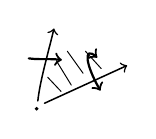
\begin{tikzpicture}[x=1cm,y=1cm,line cap=round,line join=round]
\fill (0,0) circle[radius=.025];
\draw[->,line width=.55pt] (.015,.10) .. controls (.04,.35) and (.16,.76) .. (.22,1.02);
\draw[->,line width=.55pt] (.10,.07)--(1.15,.55);
\draw[line width=.35pt] (.14,.40)--(.31,.22)
 (.25,.61)--(.44,.30)
 (.39,.73)--(.59,.45)
 (.62,.73)--(.82,.51);
\draw[->,line width=.8pt] (-.10,.64) .. controls (.03,.62) and (.14,.64) .. (.32,.62);
\draw[<->,line width=.8pt] (.77,.65) .. controls (.59,.80) and (.62,.56) .. (.81,.23);
\end{tikzpicture}}
) avec les relations génératrices
\[
(25)\qquad
\left\{\begin{aligned}
\unsure{(\sigma_0')^2}&=\unsure{(\sigma_1')^2}=\unsure{(\sigma_2')^2}
=\unsure{(\sigma_2'\sigma_0')^2}=1\\
\unsure{\bigl(\underbrace{\sigma_1'\sigma_0'}_{\rho_f}\bigr)^3}&=1
\end{aligned}\right.
\]

\margin{on pourrait aussi noter $\unsure{\sigma_\infty'}$ au lieu de $\unsure{\sigma_2'}$.
On aurait mieux fait de les noter \inserted{\unsure{ici}} carrément $r_0,r_1,r_\infty$ (au lieu de $\sigma_0,\sigma_1,\sigma_2$).}

Le sous-groupe \inserted{$\Pi_{0,3}'$} d'indice 2 \deleted{\illegible{1}}\inserted{(groupe cart. \unsure{triangul'} orienté)} est engendré par
\[
\unsure{\sigma_1'\sigma_0'}=\rho_f\inserted{\unsure{=\ell_\infty'}},\qquad
\unsure{\sigma_2'\sigma_1'}=\rho_s\inserted{\unsure{=\ell_0'}},\qquad
\unsure{\sigma_0'\sigma_2'}=\unsure{\sigma'|\sigma}\inserted{\unsure{=\ell_1'}},
\]
avec les relations génératrices
\[
(26)\qquad
\rho_f\sigma\rho_s\deleted{\unsure{\rho_s}}=1
\qquad
\sigma^2=\rho_f^3=1
\]
C'est donc le quotient de $\Pi_{0,3}$ par $\ell_1^2,\ell_\infty^3$
\[
(\unsure{27|17})\qquad
\left\{\begin{array}{rcl}
\Pi_{0,3}&\longrightarrow&\Pi_{0,3}'\\
\ell_0&\longmapsto&\ell_0'=\rho_s\\
\ell_1&\longmapsto&\ell_1'=\sigma\\
\ell_\infty&\longmapsto&\ell_\infty'=\rho_f
\end{array}\right.
\qquad,
\]
\deleted{\illegible{1}} Cet homomorphisme se prolonge en

\deleted{\unsure{(28)|(27)}}

\margin{89}
% ===== LM_P068-069: second pass, checked against the scans =====
\scanpage{91}

\[
(28)\quad
\left\{\begin{aligned}
\widetilde{\Pi}_{0,3}=\Pi_{0,3}\cdot\{1,\tau\}&\longrightarrow\widetilde{\Pi}'_{0,3}\\
\tau_0,\tau_1,\tau_\infty&\longmapsto
\sigma'_0,\sigma'_1,\sigma'_\infty
\end{aligned}\right.
\]

Ceci posé, on définit un \uline{iso.} \deleted{\illegible{1}}
\[
(29)\quad
\begin{aligned}
\widetilde{\Pi}'_{0,3}&\xrightarrow{\sim}\mathfrak S_{0,3}\\
(\sigma'_0,\sigma'_1,\sigma'_\infty)
&\longrightarrow
\left(\deleted{\unsure{\sigma^{\prime}_1}}
\underset{\substack{\inserted{\text{sur }\dot\tau'_\infty}\\\Vert\\\inserted{\dot\sigma_\infty\tau}}}{\tau'_\infty},
\underset{\substack{\inserted{\text{sur }\dot\tau'_0}\\\Vert\\\inserted{\dot\sigma_0\tau}}}{\tau'_0},
\underset{\inserted{\text{sur }\tau}}{\tau_\infty}\right)
\end{aligned}
\]
notés aussi $r_0,r_1,r_\infty$ (\uline{réflexions} fondamentales)

\margin{Cet iso. est associé à un homomorphisme canonique
$\varphi:\widetilde{\Pi}_{0,3}=\Pi_{0,3}\cdot\{1,\tau\}\xrightarrow{\text{épi}}\mathfrak S_{0,3}$
induisant un hom. can.
$\varphi:\Pi_{0,3}\xrightarrow{\text{épi}}\mathfrak S_{0,3}^{+}$
permettant d'identifier $\mathfrak S_{0,3}$ et $\mathfrak S_{0,3}^{+}$
aux quotients des pr.~\unsure{mbres.|membres} par les relations
$\ell_1^2=\ell_\infty^3=1$ \ldots}

qui induit un iso.
\[
(30)\quad
\left\{\begin{aligned}
\Pi'_{0,3}&\xrightarrow{\sim}\deleted{\unsure{\Pi}}\mathfrak S_{0,3}^{+}\\
\rho_s=\ell'_0&\longmapsto\varepsilon_0=\sigma_\infty\rho\\
\sigma=\ell'_1&\longmapsto\sigma_\infty\\
\rho_f=\ell'_\infty&\longmapsto\rho^{-1}
\end{aligned}\right.
\]

\margin{\uline{NB}
$\left\{\begin{aligned}
\tau_\infty\tau'_0&=\varepsilon_0=\ell'_0\\
\tau'_\infty\tau_\infty&=\sigma_\infty=\ell'_1\\
\tau'_0\tau'_\infty&=\rho^{-1}=\ell'_\infty
\end{aligned}\right.$
i.e.
$\begin{aligned}
r_\infty r_1&=\ell'_0\;(=\varepsilon_0)\\
r_0r_\infty&=\ell'_1\;(=\sigma_\infty)\\
r_1r_0&=\ell'_\infty\;(=\rho^{-1})
\end{aligned}$}

On trouve donc que $\mathfrak S_{0,3}$ a des \deleted{\unsure{gén}} relations génératrices
\[
(31)\quad
{\tau'_\infty}^{2}={\tau'_0}^{2}=\tau_\infty^2
=\bigl(\underbrace{\tau'_\infty\tau_\infty}_{\sigma_\infty}\bigr)^2
=\bigl(\underbrace{\tau'_0\tau'_\infty}_{\rho^{-1}}\bigr)^3=1,
\]
et $\mathfrak S_{0,3}^{+}$ a des relations génératrices
\[
(32)\quad \ell'_\infty \ell'_1\ell'_0={\ell'_1}^{2}={\ell'_\infty}^{3}=1
\]
ou aussi simplement, en éliminant $\ell'_0$ et posant
$\ell'_1=\sigma_\infty$ et ${\ell'_\infty}^{-1}=\rho$
\[
(33)\quad\boxed{\sigma_\infty^2=\rho^3=1}
\]

Pour mémoire, on va exprimer les éléments remarquables de $\mathfrak S_{0,3}^{+}$ en termes de $\sigma_\infty,\rho$ :
\scanpage{92}
\mspage{335}

\[
(34)\quad\left\{\begin{aligned}
\varepsilon_0&=\sigma_\infty\rho\ \deleted{\illegible{1}}&
\ell_0&=\sigma_\infty\rho\sigma_\infty\rho=(\sigma_\infty\rho)^2\\
\varepsilon_1&=\rho\sigma_\infty&
\ell_1&=\rho\sigma_\infty\rho\sigma_\infty=(\rho\sigma_\infty)^2\\
\varepsilon_\infty&=\rho^{-1}\sigma_\infty\rho^{-1}&
\ell_\infty&=(\rho^{-1}\sigma_\infty\rho^{-1})^2
=\rho^{-1}\sigma_\infty\rho^{-1}\sigma_\infty\rho^{-1}
\end{aligned}\right.,
\]
\[
(35)\quad\left\{\begin{aligned}
\sigma_0&=\rho^{\deleted{\unsure{2}}}\sigma_\infty\rho^{\deleted{\unsure{2}}-1}
\quad(=\deleted{\unsure{\rho}}\varepsilon_1\rho^{-1}=\rho\varepsilon_1^{-1})\\
\sigma_1&=\rho^{-1}\sigma_\infty\rho^{\deleted{\unsure{2}}}
\quad(=\rho^{-1}\varepsilon_0\deleted{\unsure{\rho}}=\varepsilon_\infty\rho^{-1})
\end{aligned}\right.
\]

et dans $\mathfrak S_{0,3}^{-}$ on a, en fonction de $\tau'_\infty,\tau'_0,\tau_\infty$,
les expressions de \deleted{$\unsure{\tau_0,\tau_1,\tau_\infty,\tau'_0,\tau'_1,\tau'_\infty}$}
\inserted{$\tau_0,\tau_1,(\tau_\infty,\tau'_0),\tau'_1,(\tau'_\infty)$}
\[
(36)\quad\left\{\begin{aligned}
\tau_0&=\deleted{\unsure{\tau_0\tau'_0\tau_\infty\tau'_\infty}}\rho\tau_\infty\rho^{-1}
=\tau'_\infty\tau'_0\tau_\infty\tau'_0\tau'_\infty
\quad(=r_0r_1r_\infty r_1r_0)\\
\tau_1&=\rho^{-1}\tau_\infty\rho
=\tau'_0\tau'_\infty\tau_\infty\tau'_\infty\tau'_0
\quad(=r_1r_0r_\infty r_0r_1)\\
\tau'_1&=\rho\tau'_0\rho^{-1}
=\tau'_\infty\deleted{\unsure{\tau'_0}}\tau'_0\tau'_\infty
\quad(=r_0r_1r_0)
\end{aligned}\right.
\]
et
\[
\left\{\begin{aligned}
\tau'_\infty&=r_0\\
\tau'_0&=r_1\\
\tau_\infty&=r_\infty.
\end{aligned}\right.
\]

\uline{IV}) Relation avec
$\mathrm{Gl}(2,\mathbb Z)'=\mathrm{Gl}(2,\mathbb Z)/\mathord{\pm}1
\simeq\mathrm{GP}(1,\mathbb Z)$.

Ce groupe opère sur le demi-plan de Poincaré
\[
D=\{z\in\mathbb C\mid\Im z>0\}
\]
par
\[
(37)\quad\left\{\begin{aligned}
u_g(z)&=\frac{az+b}{cz+d}&\text{si }ad-bc&=+1\\
u_g(z)&=\frac{a\bar z+b}{c\bar z+d}&\text{si }ad-bc&=-1
\end{aligned}\right.
\qquad
\begin{gathered}
g=\begin{pmatrix}a&b\\c&d\end{pmatrix}\\
a,b,c,d\in\mathbb Z\\
ad-bc\in\{\pm1\}
\end{gathered}
\]

On a dans $D$ un domaine fondamental hachuré, qui correspond au triangle
sphérique $(-\bar j,0,\tfrac12)$ par l'\unsure{homomorphisme|homéomorphisme}
de \unsure{revêt.} naturel, $i$ correspondant à $\tfrac12$,
$-\bar j$ à $-\bar j$, et le point à l'infini à $0$.
\deleted{Ainsi \unsure{on trouve}}\inserted{Les réflexions}
par rapport aux trois côtés de ce triangle sont donnés par
\[
(38)\quad
\deleted{\unsure{\tau_0}}\unsure{r_0|\tau_0}(z)=\frac1{\bar z},\qquad
\unsure{r_1|\tau_1}(z)=1-\bar z,\qquad
\unsure{r_\infty|\tau_\infty}(z)=-\bar z
\]
\figure{\begin{tikzpicture}[x=2.2cm,y=2.2cm,line cap=round,line join=round,font=\scriptsize]
\draw[line width=.4pt] (-1.55,0) .. controls (-.7,.04) and (.5,-.025) .. (1.85,.01);
\draw[line width=.4pt] (-1,0) arc[start angle=180,end angle=0,radius=1];
\draw[line width=.5pt] (0,-.48)--(0,2.85);
\draw[line width=.5pt] (.5,-.65)--(.5,2.78);
\begin{scope}
\clip (0,1) arc[start angle=90,end angle=60,radius=1]--(.5,2.78)--(0,2.85)--cycle;
\foreach \h in {.96,1.24,1.52,1.80,2.08,2.36,2.64}
  \draw[line width=.35pt] (0,\h)--(.5,{\h+.30});
\end{scope}
\draw[line width=.7pt] (0,1)--(.075,1)--(.075,1.075)--(0,1.075);
\fill (.5,.8660254) circle[radius=.025];
\node[inner sep=0pt] at (-1.04,-.14) {$-1$};
\node[inner sep=0pt] at (-.10,-.14) {$0$};
\node[inner sep=0pt] at (.43,-.18) {$\frac12$};
\node[inner sep=0pt] at (1.04,-.14) {$1$};
\node[inner sep=0pt] at (-.13,1.12) {$i$};
\node[inner sep=0pt] at (.64,.94) {$-\bar j$};
\node[inner sep=0pt,anchor=east,rotate=16] at (-.07,1.94) {$\dot r_\infty=\dot\tau_\infty$};
\node[inner sep=0pt,anchor=west] at (.56,2.25) {$\dot\tau'_0=\dot r_1$};
\node[inner sep=0pt,rotate=-63] at (.23,.63) {$\dot\tau'_\infty=\dot r_0$};
\end{tikzpicture}}

\deleted{\unsure{Ils déterminent}} et les produits deux à deux de ces réflexions
\scanpage{93}

sont
\[
(39)\quad\left\{\begin{aligned}
\unsure{r_\infty r_1|\tau_\infty\tau_1}(z)&=\ell'_0(z)=z-1\;\deleted{\unsure{;}}\\\unsure{r_0r_\infty|\tau_0\tau_\infty}(z)&=\ell'_1(z)=-\frac1z\\
\unsure{r_1r_0|\tau_1\tau_0}(z)&=\ell'_\infty(z)=1-\frac1z=\frac{z-1}{z}
\end{aligned}\right.
\]

On trouve ainsi un isomorphisme
\[
(40)\quad\left\{\begin{aligned}
\mathfrak S_{0,3}&\xrightarrow{\sim}\mathrm{Gl}(2,\mathbb Z)'\simeq
\mathrm{Gl}(2,\mathbb Z)/\mathord{\pm}1\simeq\mathrm{GP}(1,\mathbb Z)\\
r_0=\tau'_\infty&\longmapsto r_0=\begin{pmatrix}0&1\\1&0\end{pmatrix}\\
r_1=\tau'_0&\longmapsto r_1=\begin{pmatrix}-1&1\\0&1\end{pmatrix}\\
r_\infty=\tau_\infty&\longmapsto r_\infty=\begin{pmatrix}1&0\\0&-1\end{pmatrix}
\end{aligned}\right.
\]
\margin{il vaut mieux changer \unsure{des|de} signes \unsure{cf. Formulaire|cf formulaire}}

et une présentation de $\mathrm{GP}(1,\mathbb Z)$ par
\[
(41)\quad r_0^2=r_1^2=r_\infty^2=(r_0r_\infty)^2=(r_1r_0)^3=1.
\]
Cet iso. induit un iso
\[
(42)\quad\left\{\begin{aligned}
\mathfrak S_{0,3}^{+}&\xrightarrow{\sim}
\mathrm{Sl}(2,\mathbb Z)'=\mathrm{Sl}(2,\mathbb Z)/\mathord{\pm}1
\simeq\mathrm{GP}(1,\mathbb Z)^{+}\\
\ell'_1=\sigma_\infty&\longmapsto\begin{pmatrix}0&-1\\1&0\end{pmatrix}\\
\ell'_\infty=\rho^{-1}&\longmapsto\begin{pmatrix}1&-1\\1&0\end{pmatrix}
\end{aligned}\right.
\]
\[
(\text{d'où}\quad\rho\longmapsto\begin{pmatrix}0&1\\-1&1\end{pmatrix}).
\]

On identifie par la suite les éléments de $\mathfrak S_{0,3}$ avec leurs images dans
$\unsure{\mathrm{Gl}|\mathrm{Sl}}(2,\mathbb Z)'\simeq\mathrm{GP}(1,\mathbb Z)$.
Notons le formulaire suivant \unsure{(où on utilise} que pour une matrice
$u=\begin{pmatrix}a&b\\c&d\end{pmatrix}\in\mathrm{Sl}(2,\mathbb Z)$,
\deleted{\illegible{1}}
\deleted{\unsure{pour} $\det u\in\mathbb Z^*=\{\pm1\}$ donc $(\det u)^2=1$}, on a
\scanpage{94}
\mspage{336}

\[
(43)\quad u^{-1}=\begin{pmatrix}d&-b\\-c&a\end{pmatrix}\quad):
\]

\margin{NB. \unsure{2.} \deleted{\unsure{Si det}} $u\in\mathrm{Gl}(2,A)$,
$A$ anneau \unsure{quelc.}, on a
$\det(u)\cdot u^{-1}=\begin{pmatrix}d&-b\\-c&a\end{pmatrix}$}

\deleted{\unsure{Et}}.
\[
(44)\quad\left\{\begin{aligned}
\varepsilon_0=\sigma_\infty\rho&=\begin{pmatrix}1&-1\\0&1\end{pmatrix},&
\varepsilon_0^{-1}&=\begin{pmatrix}1&1\\0&1\end{pmatrix}\\
\varepsilon_1=\rho\sigma_\infty&=\begin{pmatrix}1&0\\1&1\end{pmatrix},&
\varepsilon_1^{-1}&=\begin{pmatrix}1&0\\-1&1\end{pmatrix}\\
\varepsilon_\infty=\rho^{-1}\sigma_\infty\rho^{-1}&=\begin{pmatrix}2&-1\\1&0\end{pmatrix},&
\varepsilon_\infty^{-1}&=\begin{pmatrix}0&1\\-1&2\end{pmatrix}\\
\ell_0=\varepsilon_0^2&=\begin{pmatrix}1&-2\\0&1\end{pmatrix}&
\sigma_0&=\begin{pmatrix}1&-1\\2&-1\end{pmatrix}\\
\ell_1=\varepsilon_1^2&=\begin{pmatrix}1&0\\2&1\end{pmatrix}&
\sigma_1&=\begin{pmatrix}1&-2\\1&-1\end{pmatrix}\\
\ell_\infty=\varepsilon_\infty^2&=\begin{pmatrix}3&-2\\2&-1\end{pmatrix}&
\sigma_\infty&=\begin{pmatrix}0&-1\\1&0\end{pmatrix}
\end{aligned}\right.
\]
\margin{Cf. ``formulaire'' pour liste des relations et d'écritures plus \unsure{complète}.}
\[
(45)\quad\rho=\begin{pmatrix}0&1\\-1&1\end{pmatrix},\qquad
\unsure{\rho^{-1}|\rho^{-1\prime}}=\begin{pmatrix}1&-1\\1&0\end{pmatrix},
\]
\[
(46)\quad \ell_\infty \ell_1\ell_0=\begin{pmatrix}-1&0\\0&-1\end{pmatrix}
\]
l'élément non trivial du centre de $\mathrm{Sl}(2,\mathbb Z)$ qui
(heureusement!) donne $1$ dans $\mathrm{Sl}(2,\mathbb Z)'$

Le groupe $\Pi_{0,3}$ se récupère comme le noyau de l'homomorphisme
\diagram{\begin{tikzcd}[ampersand replacement=\&]
\mathrm{Sl}(2,\mathbb Z)' \arrow[r] \& \mathrm{Sl}(2,\mathbb Z/2\mathbb Z) \arrow[d,phantom,"\simeq"{description,rotate=90}]\\
\& \mathfrak S_3
\end{tikzcd}}
la suite exacte
\[
(47)\quad
\diagram{\begin{tikzcd}[ampersand replacement=\&]
1 \arrow[r] \& \Pi_{0,3}\arrow[r,dash] \& \mathfrak S_{0,3}^{+}\arrow[r,dash] \& \mathcal{T}_{0,3}^{+\unsure{\prime}}\arrow[r,dash]\arrow[d,phantom,"\simeq"{description,rotate=90}] \& 1\\
\&\&\&\mathfrak S_3\&
\end{tikzcd}}
\]
se récupère comme
\[
(48)\quad
\diagram{\begin{tikzcd}[ampersand replacement=\&]
1\arrow[r]\&\Pi(2)'\arrow[r]\arrow[d,phantom,"\simeq"{description,rotate=90}] \& \mathrm{Sl}(2,\mathbb Z)'\arrow[r] \& \mathrm{Sl}(2,\mathbb Z/2\mathbb Z)\arrow[r]\arrow[d,phantom,"\simeq"{description,rotate=90}] \& 1\\
\&\Pi_{0,3}^{\unsure{\beta}}\&\&\mathfrak S_3\&
\end{tikzcd}}
\]
\scanpage{95}

Ça nous fourmille dans \unsure{les mains|la main} de \deleted{\unsure{rigoler}}\inserted{travailler}
dans $\mathrm{Gl}(2,\mathbb Z)$ lui-$\overline{\mathrm m}$, extension centrale de
$\mathfrak S_{0,3}$ --- en fait, cette extension s'interprète comme
$\mathcal{T}_{1,1}$ --- mais nous y reviendrons, ultérieurement\ldots

\uline{V}) Résumons les avatars du $\overline{\mathrm m}$ groupe, que nous avons
\unsure{rencontrés|rencontré} jusqu'à présent

1) $\mathfrak S_{0,3}\overset{\text{dfn}}{=}\operatorname{Aut}_{\mathrm{lac}}(\Pi_{0,3})$
avec \unsure{ss-groupe} $\mathfrak S_{0,3}^{+}$ (respectant orientation)

2) $\mathcal{T}'_{0,4}\simeq\operatorname{Autext}_{\mathrm{lac}}(\Pi_{0,4})'$
aut ext. de $\Pi_{0,4}$ respectant la structure à lacets et fixant la classe de lacets
$\unsure{L_4|L_\lambda}$ (et permutant $L_0,L_1,\unsure{L_\infty|L_3}$)

\deleted{avec $\unsure{\mathcal{T}_{0,4}^{\prime+}}$}
\deleted{$\unsure{A'_{0,4}/A_{0,4}^{\prime0}}\simeq\unsure{\operatorname{Auttop}}(\mathbb P^1_{\mathbb C}\setminus\{0,\unsure{1}\})$}
avec $\mathcal{T}_{0,4}^{\prime+}$ (respectant orientation)

3) $A'_{0,4}/A_{0,4}^{\prime0}$ groupe des composantes connexes de
\[
A'_{0,4}\subset\operatorname{Auttop}
\left(\deleted{\mathbb P^1_{\mathbb C}\setminus\unsure{\{}}
\underset{\substack{\Vert\\\mathbb P^1_{\mathbb C}\setminus\{0,1,\infty;\tfrac12\}}}{U_{0,4}^{\mathrm{top}}}\right)
\]
sous-groupe des autom. qui fixent le point à l'infini $a_{0,4}=\tfrac12$

avec $A_{0,4}^{\prime+}/A_{0,4}^{\prime0}$ (respectant orientation

4) $\Pi_1\bigl((U_{0,3}^{\mathrm{an}},\overbrace{\mathfrak S_3\times\unsure{\mathbb Z_2|\mathbb Z/2}}^{\mathcal{T}_{0,3}}),-\bar j\bigr)$
(décrit à la J. Malgoire)
avec le sous-groupe $\Pi_1\bigl((U_{0,3}^{\mathrm{an}},\mathfrak S_3),-\bar j\bigr)$
$(\mathfrak S_3=\mathcal{T}_{0,3}^{+})$

5) $\Pi_1\bigl((\mathbb P^{1\,\mathrm{an}}_{\mathbb C},0\cdot\{0\}+2\{1\}+3\{\infty\}),-\bar j\bigr)$
(à la J. Malgoire)
avec le sous-groupe $\Pi_1\bigl(\mathbb P^{1\,\mathrm{an}}_{\mathbb C},\unsure{0}\{0\}+2\{1\}+3\{\infty\}\bigr)$

6) Groupe cartographique triangulé \deleted{\illegible{1}} $\Gamma_{\infty,3}$
\[
\Gamma_{\infty,3}\unsure{\}}=\{r_0,r_1,r_\infty\mid
r_0^2=r_1^2=r_\infty^2=(r_0r_\infty)^2=(r_1r_0)^3=1\}
\]
(avec sous-groupe cart. triangulé orienté
\[
\Gamma_{\infty,3}^{\circ}=\{
\underset{\substack{\Vert\\r_\infty r_1}}{\rho_s},
\underset{\substack{\Vert\\r_0r_\infty}}{\sigma},
\underset{\substack{\Vert\\r_1r_0}}{\rho_f}
\mid\rho_f\sigma\rho_s=\sigma^2=\rho_f^3=1\}.
\]
)

\margin{c'est aussi le groupe
$\widetilde{\Pi}_{0,3}/(\ell_1^2,\ell_\infty^3)$, où
$\widetilde{\Pi}_{0,3}=\Pi_{0,3}\cdot\{1,\tau\}$}

7) $\Pi_1\bigl(\mathcal U_{0,3}^{\mathrm{conf}},\operatorname{pt}(U_{0,3},-\bar j)\bigr)$
\inserted{surface conforme universelle de type $(0,3)$}
avec sous-groupe $\Pi_1\bigl(\mathcal U_{0,3}^{\mathrm{an}},\operatorname{pt}(U_{0,3},-\bar j)\bigr)$
\inserted{surface holomorphe universelle de type $(0,3)$}

\margin{\uline{NB} $\mathcal U_{0,3}^{\mathrm{conf}}\simeq(U_{0,3},\mathcal T_{0,3})$
ce qui permet d'identifier 7) à 4)}

8) $\mathcal T'_{1,1}=\mathcal T_{1,1}/\underbrace{\{\pm1\}}_{\text{centre}}$,
avec $\mathcal T_{1,1}\simeq\operatorname{Autext}_{\mathrm{lac}}(\Pi_{1,1})
\simeq A_{1,1}/A_{1,1}^{0}$

($A_{1,1}\simeq\text{autom. top. de }\unsure{U_{1,1}^{\circ}|U_{1,1}}$)
avec sous groupe $\mathcal T_{1,1}^{\prime+}=\mathcal T_{1,1}^{+}/\{\pm1\}$
\scanpage{96}
\mspage{337}

9) $\Pi_1(M_{1,1}^{\mathrm{conf}},\mathrm{pt})' \simeq \unsure{\Pi_1()/\mathrm{centre}\{\pm1\}} \simeq \Pi_1(M_{1,1}'{}^{\mathrm{conf}},\mathrm{pt})$

où $M_{1,1}^{\mathrm{an}}$ est la multiplicité modulaire \deleted{analytique}\inserted{\unsure{conf|conf.}} des courbes elliptiques \inserted{conformes} (i.e. courbes \deleted{analytiques}\inserted{conformes} de type $1,1$), $M_{1,1}'{}^{\mathrm{an}}$ celle des courbes elliptiques \deleted{analytiques}\inserted{conformes} ``mod. symétrie''; avec sous-groupe
\[
\Pi_1(M_{1,1}^{\mathrm{an}},\mathrm{pt})' \simeq \unsure{\Pi_1()/\mathrm{centre}\{\pm1\}} \simeq \Pi_1(M_{1,1}'{}^{\mathrm{an}},\mathrm{pt})
\]
où le pt base est la courbe \inserted{ell. conforme \unsure{resp.}} analytique, quotient de $\mathbb C$ par $\mathbb Z+\mathbb Z(-\bar j)$. \uline{NB} Les multiplicités modulaires sont $(D,\mathrm{Gl}(2,\mathbb Z))$, $(D,\mathrm{Sl}(2,\mathbb Z))$ dans le cadre \deleted{analytique} conforme resp. analytique pour $M_{1,1}$, et $(D,\mathrm{Gl}(2,\mathbb Z)'=\mathrm{GP}(1,\mathbb Z))$ resp. $(D,\unsure{\mathrm{Sl}(1,\mathbb Z)'|\mathrm{Sl}(2,\mathbb Z)'}=\mathrm{GP}(1,\mathbb Z)^+)$ dans le cadre conforme resp. analytique pour $M_{1,1}'$.

10) $\mathrm{Gl}(2,\unsure{\mathbb Z^{\ast}|\mathbb Z})' \simeq \mathrm{GP}(1,\mathbb Z)$, avec le sous-groupe $\mathrm{Sl}(2,\mathbb Z)'\simeq\mathrm{GP}(1,\mathbb Z)^+$.
\scanpage{97}

(VI) \uline{Les automorphismes à lacets de} $\widehat{\Pi}_{0,3}$ \uline{et de} $\widehat{\mathfrak S}_{0,3}^{+}$

On a un diagramme \unsure{comm.} canonique :

(49)
\diagram{\begin{tikzcd}[ampersand replacement=\&,column sep=large,row sep=large]
\begin{array}{l}
\operatorname{Autext}(\widehat{\mathfrak S}_{0,3}^{+})'\\
=\text{groupe des autom}\\
\text{ext. induisant}\\
\text{l'identité dans le}\\
\text{quotient }\mathfrak S_3\simeq\mathcal T_{0,3}^{+}
\end{array}
\arrow[r,"{\text{restriction}}","\sim"']
\&
\begin{array}{l}
\operatorname{Autext}^{\unsure{\rho}}(\widehat{\Pi}_{0,3})'\\
=\text{groupe des autom}\\
\text{extérieurs qui}\\
\text{commutent à}\\
\text{l'action ext. de }\mathfrak S_3
\end{array}
\\
\begin{array}{l}
\operatorname{Aut}(\widehat{\mathfrak S}_{0,3}^{+},\sigma_\infty)'\\
=\text{groupe des autom}\\
\text{de }\widehat{\mathfrak S}_{0,3}^{+}\text{ qui }\deleted{\unsure{\text{fixent}}}\inserted{\text{fixent}}\ \sigma_\infty,\\
\text{et qui fixent }\rho\ \mathrm{mod}\ \widehat{\Pi}_{0,3}
\end{array}
\arrow[u,"\sim"]\arrow[r,"{\text{restriction}}","\sim"']
\&
\begin{array}{l}
\operatorname{Aut}(\widehat{\Pi}_{0,3},\sigma_\infty)\\
=\text{groupe des aut.}\\
\text{qui commutent}\\
\text{à }\sigma_\infty,\text{ et qui}\\
\text{commutent}\\
\mathrm{ext}^{\mathrm t}.\text{ à }\rho
\end{array}
\arrow[u,"\sim"]
\end{tikzcd}}

\margin{\deleted{\illegible{1}}}

Les \unsure{$\in$} \deleted{\unsure{éléments}} $\operatorname{Aut}(\widehat{\mathfrak S}_{0,3}^{+},\sigma_\infty)'$ sont de la forme
\[
(50)\qquad
\left\{\begin{aligned}
u(\sigma_\infty)&=\sigma_\infty\\
u(\rho)&=g\rho
\end{aligned}\right.
\qquad (\text{i.e. }u\rho u^{-1}\rho^{-1}=g)
\]

\margin{On écrit les formules dans $\operatorname{Aut}(\widehat{\mathfrak S}_{0,3}^{+})'=G$, groupe des autom de $\widehat{\mathfrak S}_{0,3}^{+}$ qui induisent l'identité dans $\widehat{\mathfrak S}_{0,3}^{+}/\Pi_{0,3}\simeq\mathfrak S_3$, \uline{\unsure{s'identifie}} au groupe $\operatorname{Aut}(\Pi_{0,3})'=\mathrm{gr.}$ des autom de $\Pi_{0,3}$ qui commutent \inserted{\unsure{\uline{extérieure}}} à $\mathfrak S_3$; -- on aura $\Pi_{0,3}\subset\widehat{\mathfrak S}_{0,3}^{+}\subset\widehat{\mathfrak S}_{0,3}\subset\unsure{\mathfrak g.|g.}\,G$. \uline{NB} On admet ici que le centre de $\widehat{\mathfrak S}_{0,3}^{+}$ est trivial.}

$g\in\widehat{\Pi}_{0,3}$ \deleted{\illegible{1}} est assujetti à la condition de cocycle
\[
(51)\qquad \boxed{g\rho(g)\rho^2(g)=1}
\]
qui exprime la relation
\[
(52)\qquad (g\rho)^3=1\ .
\]

On trouve ainsi une corr. $1-1$ entre les éléments de $\operatorname{Aut}(\widehat{\mathfrak S}_{0,3}^{+},\sigma_\infty)'$ et les $g\in\widehat{\Pi}_{0,3}$ \unsure{satisfaisant} (51), et tels de plus que

(53) $\sigma_\infty,g\rho$ avec les relations $\sigma_\infty^2=(g\rho)^3=1$ \unsure{présentent} $\widehat{\mathfrak S}_{0,3}^{+}$
\scanpage{98}
\mspage{338}

(que je vais appeler la ``condition liminaire'').

\deleted{Pour \unsure{$u$ ainsi défini par un}}

Pour un $u\in G=\operatorname{Aut}(\widehat{\mathfrak S}_{0,3}^{+})'\unsure{!}$ (ne fixant pas nécessairement $\sigma_\infty$), on a des conditions équivalentes
\[
(54)\quad
\left\{\begin{aligned}
\text{(i)}\quad &u(\overset{\inserted{\varepsilon_0}}{\ell'_0})\in\text{conjugué de }\deleted{\unsure{\ell}}\varepsilon_0^{\widehat{\mathbb Z}}=L'_0\ (\text{dans }\widehat{\mathfrak S}_{0,3}^{+})\\
\text{(ii)}\quad &u(\ell_0)\in\text{conjugué de }\ell_0^{\widehat{\mathbb Z}}=L_0\ (\text{dans }\widehat{\Pi}_{0,3})\\
\text{(iii)}\quad &u(L_i)\text{ conjugué de }L_i\quad\text{pour }i=0,1,\infty\\
\text{(iv)}\quad &\exists\ p\in\widehat{\mathbb Z}^{\ast},\ g_0\in\widehat{\Pi}_{0,3}\quad
\boxed{u(\varepsilon_0)=\operatorname{int}(g_0)\varepsilon_0^p}\\
\text{(v)}\quad &\exists\ p\in\widehat{\mathbb Z}^{\ast},\ g_0\in\widehat{\Pi}_{0,3}\quad
\boxed{u(\ell_0)=\operatorname{int}(g_0)(\ell_0^p)}
\end{aligned}\right.
\]

On aura alors aussi
\[
(55)\qquad
\begin{aligned}
\deleted{\unsure{u}}\quad u(\ell_1)&=\operatorname{int}(g_1)(\ell_1^p)&
g_1&=g\rho(g_0)\\
u(\ell_\infty)&=\operatorname{int}(g_\infty)(\ell_\infty^p)&
g_\infty&=g\rho(g_1)=g\rho(g)\rho^2(g_0)\ .
\end{aligned}
\]

L'élément \deleted{$p\in\widehat{\mathbb Z}^{\ast}$ \unsure{est}}
\[
(55)\qquad p\in\widehat{\mathbb Z}^{\ast}\qquad p=\chi(u)
\]
est bien déterminé par $u$, donc par $g$\inserted{(si $u$ donné par (50))}, on l'appellera le \uline{multiplicateur} de $u$. L'élément \deleted{\unsure{$g_0$}}
\[
(56)\qquad g_0\in\widehat{\Pi}_{0,3}
\]
est déterminé a priori mod $L_0=\ell_0^{\widehat{\mathbb Z}}$ (changement
\[
(57)\qquad g_0\longmapsto g_0\ell_0^\alpha
\]
).

\margin{Notations $\operatorname{Autext}_{\mathrm{lac}}(\widehat{\mathfrak S}_{0,3}^{+})$, $\operatorname{Aut}_{\mathrm{lac}}(\widehat{\mathfrak S}_{0,3}^{+})$, $\operatorname{Aut}_{\mathrm{lac}}(\widehat{\mathfrak S}_{0,3}^{+})'$, $\operatorname{Aut}_{\mathrm{lac}}(\widehat{\mathfrak S}_{0,3}^{+},\sigma_\infty)'$, $\operatorname{Aut}_{\mathrm{lac}}(\widehat{\Pi}_{0,3},\sigma_\infty)\ldots$}

Si les conditions \inserted{équiv.} (\unsure{54|55}) sont satisfaites, on dit que $u$ respecte la structure à lacets de $\widehat{\mathfrak S}_{0,3}^{+}$ (ou de $\Pi_{0,3}$) -- en sous-entendant que $\widehat{\mathfrak S}_{0,3}^{+}$ est muni du ``groupe-lacet'' $\varepsilon_0^{\widehat{\mathbb Z}}\simeq L'_0$. On se \unsure{bornera|borne} par la suite à de tels autom. \uline{NB} Ces conditions ne dépendent que de l'autom. ext. défini par $u$, dans $\widehat{\Pi}_{0,3}$ ou dans $\widehat{\mathfrak S}_{0,3}^{+}$. On
\scanpage{99}

va \unsure{s'intéresser} aux relèvements canoniques de tels autom extérieurs donnés par (49), (50), en des autom. effectifs.

La formule de définition (50) de $u$ ne fait intervenir que $g$\inserted{$\in\widehat{\Pi}_{0,3}$}, en principe $g_0\ \mathrm{mod}\ L_0$ dans $\widehat{\Pi}_{0,3}/L_0$ est déduit de $g$. Mais en pratique $g_0$ joue un rôle aussi important que $g$ -- on verra que dans une large mesure il détermine $g$ (formule (62)).

S'il n'y avait pas lieu d'introduire $g_0$, pour exprimer les conditions (54), on pourrait aisément \uline{paramétrer} les $g$ \unsure{satisfaisant} (51) -- donc correspondants à des \deleted{\unsure{scindages de}}\inserted{relèvements de} $\dot\rho\in\mathfrak S_3$ en des éléments d'ordre $3$ de $\widehat{\mathfrak S}_{0,3}^{+}$ -- en notant qu'il y a exactement deux classes de conjugaison de tels relèvements, (correspondant aux pts fixes $-\bar j,-j$ de $\dot\rho$ opérant sur $U_{0,3}^{\mathrm{an}}$), qui se paramétrisent par
\[
(58)\quad
\left\{\begin{aligned}
g&=\lambda_0^{\unsure{\sharp|\ast}}\rho(\lambda_0^{\unsure{\sharp|\ast}})^{-1}
=[\lambda_0^{\unsure{\sharp|\ast}},\rho]
&&\begin{gathered}\text{(\deleted{première}\inserted{classe} principale, \unsure{correspondante|correspondant}}\\
\text{au ``pôle nord'' }-\bar j)\end{gathered}\\
g&=\lambda_0^{\unsure{\sharp|\ast}\prime}\ell_1^{-1}\rho(\lambda_0^{\unsure{\sharp|\ast}\prime})^{-1}
&&\begin{gathered}\text{(classe adjointe, corresp. au}\\
\text{``pôle sud'' }-j)\end{gathered}
\end{aligned}\right.
\]

\margin{\unsure{Ces|Les} \unsure{représentations} paramétriques sont \unsure{univoques|uniques}.}

où $\lambda_0,\lambda_0^{\unsure{\sharp|\ast}\prime}\in\widehat{\Pi}_{0,3}$. On verra plus bas que ces cas correspondent respectivement aux cas
\[
(59)\qquad p\equiv1\ (3)\qquad\text{et}\qquad p\equiv-1\ (3)\ .
\]
\scanpage{100}
\mspage{339}

Mais ici la situation se corse considérablement par la nécessité de tenir compte des \deleted{\unsure{la|les}} conditions (54) (p.ex. sous la forme (iv)) -- donc \inserted{celle} d'introduire conjointement $g_0,p$. Il y a lieu alors d'introduire les quantités
\[
(60)\qquad \gamma=\frac{p-1}{2}\in\widehat{\mathbb Z}
\]
(NB comme $p\in\widehat{\mathbb Z}^{\ast}$, sa \unsure{cl.} dans $\mathbb Z/2\mathbb Z$\inserted{$=\widehat{\mathbb Z}/2\widehat{\mathbb Z}$} est $1$, donc $p-1\in2\widehat{\mathbb Z}$, d'où la possibilité de trouver $\gamma$),
\[
(61)\qquad h_0=g_0^{-1}\sigma_\infty(g_0)
\]

\margin{$h_0$, relatif à l'autom. $\sigma_\infty$ d'ordre $2$, \unsure{joue} un rôle symétrique \unsure{de} $\xi$ relatif à l'autom. $\rho$ d'ordre $3$ -- ceci n'apparaît pas \unsure{non plus} dans les notations.}

\deleted{(on change nos notations, précédemment on avait pris $h_0=\sigma_\infty(g_0)^{-1}g_0$, donc on prend l'inverse \unsure{p.r.|p.v.} aux notations précédentes).} On vérifie \unsure{bien|donc} que $g$ s'exprime à l'aide de $g_0$ et de $\gamma$ (donc de $p$) à l'aide de la formule (\uline{équivalente} à (54) (iv) ou (v))
\[
(62)\quad
\boxed{g=\sigma_\infty(g_0)\ell_1^\gamma\rho(g_0)^{-1}}
\left(=(g_0\ell_0^{-\gamma})\left(\underbrace{\ell_0^\gamma h_0}_{\xi}\right)\rho(g_0\ell_0^{-\gamma})^{-1}\right)
\]

\margin{\uline{NB} Cette expression de $g$ n'est pas \unsure{changée} si $g_0\longmapsto g_0\ell_0^\alpha$.}

Donc les $u$ qui nous intéressent sont décrits par les couples $(g_0,\gamma)$ $(g_0\in\widehat{\Pi}_{0,3}/L_0,\ \gamma\in\widehat{\mathbb Z})$ \unsure{satisfaisant} les conditions
\[
(63)\qquad 2\gamma+1\in\widehat{\mathbb Z}^{\ast}\qquad (\mathrm{NB}\quad 2\gamma+1=p=\chi(u))
\]
et la condition (51), où $g$ est exprimé en fonction de $g_0$ et de $\gamma$ par (62). Cette \deleted{formule}\inserted{relation} (51) équivaut à son tour à la relation
\[
(64)\qquad\boxed{\xi\rho(\xi)\rho^2(\xi)=1}
\]
où
\[
(65)\quad\xi=\ell_0^\gamma h_0
\qquad\unsure{\deleted{\text{avec}}|\text{avec}}\ (66)\quad
\begin{aligned}
h_0&\overset{\mathrm{dfn}}{=}
g_0^{-1}\sigma_\infty(g_0)\\
&{}=[g_0^{-1},\sigma_\infty]
\end{aligned}
\]

\margin{\uline{NB} On \unsure{appelle} ici $h_0$ ce que précédemment on notait \unsure{$h_0^{-1}$}.}
\scanpage{101}

Ainsi, les $u$ sont \unsure{paramétrés} par les couples
$(g_0\in\widehat{\Pi}_{0,3}/L_0,\ \gamma\in\widehat{\mathbb Z})$, satisfaisant les conditions
(63) et (64), qui (moyennant (65)) s'écrit sous forme explicite
\[
\tag{\unsure{65bis}}
\boxed{
\bigl(\ell_0^\gamma\underbrace{g_0^{-1}\sigma_\infty(g_0)}_{h_0}\bigr)
\rho\bigl(\ell_0^\gamma\underbrace{g_0^{-1}\sigma_\infty(g_0)}_{h_0}\bigr)
\rho^2\bigl(\ell_0^\gamma\underbrace{g_0^{-1}\sigma_\infty(g_0)}_{h_0}\bigr)=1
}
\]
\margin{il vaudrait mieux considérer cette équation comme ``équation en $h_0$'' \unsure{jouant} un rôle symétrique à ``l'équation en $\xi$'' (68)}
(``équation en $g_0$'' --- par opposition avec l'``équation en $\xi$'' plus bas).
(De plus, il \unsure{faut} rajouter la condition liminaire, pour mémoire...)

On peut aussi considérer que \deleted{$g$ est} $u$ (via $g$) est défini par
$(\xi\in\widehat{\Pi}_{0,3},\ \gamma\in\widehat{\mathbb Z})$, qui permettent en effet de retrouver
\[
h_0=\ell_0^{-\gamma}\xi
\]
par (65), puis $g_0$ par (66)
\[
g_0^{-1}\sigma_\infty(g_0)=h_0
\]
qui détermine en effet $g_0$ de façon unique, grâce au fait (qu'on admet provisoirement)
que $\widehat{\Pi}_{0,3}^{\sigma_\infty}=\{1\}$.
La possibilité de trouver $g_0$ satisfaisant à cette condition équivaut (on l'admettra aussi ici) à la condition
\[
\tag{67}
\sigma_\infty(h_0)h_0=1
\]
qui, en termes de $\xi,\gamma$, s'écrit aussi sous la \unsure{forme}
\scanpage{102}
\mspage{340}

\[
\tag{68}
\boxed{\sigma_\infty(\xi)=\ell_1^\gamma\xi^{-1}\ell_0^\gamma}.
\]

Les équations (64), (68) sont appelées les ``équations en $\xi$'' --- par opposition à ``l'équation en $g_0$'' (66), qui à première vue a l'avantage d'être une seule, et le désavantage d'être plus \unsure{compliquée}.
\margin{plutôt ``l'équation en $h_0$''}
En résumé, les $u$ qui nous intéressent
$(u\in\mathrm{Aut}_{\mathrm{lac}}(\widehat{\mathfrak S}_{0,3}^{+},\sigma_\infty)')$
sont \unsure{donnés|décrits} par les couples
\deleted{$\unsure{(\xi,\gamma)}$}\inserted{$(\xi\in\widehat{\Pi}_{0,3}^{+},\ \gamma\in\widehat{\mathbb Z})$}, satisfaisant les conditions
\[
\begin{aligned}
\text{a)}\quad&2\gamma+1\in\widehat{\mathbb Z}^{*} &&(63)\\
\text{b)}\quad&\xi\rho(\xi)\rho^2(\xi)=1 &&(64)\\
\text{c)}\quad&\sigma_\infty(\xi)=\ell_1^\gamma\xi^{-1}\ell_0^\gamma &&(68)
\end{aligned}
\]
d) Condition liminaire pour mémoire (53)
(qui ne \unsure{s'expriment} apparemment pas directement de façon commode en termes de $\xi,\gamma$).

Pour que deux couples $(\xi,\unsure{\gamma})$, $(\xi',\unsure{\gamma}')$ définissent le $\overline{\mathrm m}$ $u$, il f. et s. qu'on ait
\[
\tag{69}
\unsure{\gamma}=\unsure{\gamma}',\qquad
\xi'=\ell_0^{-\alpha}\xi \ell_1^\alpha\qquad(\alpha\in\widehat{\mathbb Z}).
\]

La condition (64) peut encore se \unsure{remplacer} par une représentation paramétrique
\[
\tag{70}
\left\{
\begin{aligned}
\xi&=\lambda\rho(\lambda)^{-1}\qquad\text{ou}\\
\xi&=\lambda \ell_0^{-1}\rho(\lambda)^{-1}
\end{aligned}
\right.
\]
avec $\lambda\in\widehat{\Pi}_{0,3}$ --- auquel cas l'équation (68)
\scanpage{103}

peut s'interpréter comme une ``équation en $\lambda$'', qui suivant les deux cas prend la forme
\[
\tag{71}
\left\{
\begin{aligned}
\sigma_\infty(\lambda\rho(\lambda)^{-1})
 &=\ell_1^\gamma(\rho(\lambda)\lambda^{-1})\ell_0^\gamma\\
&\text{ou}\\
\sigma_\infty(\lambda\unsure{\ell_0^{-1}}\rho(\lambda)^{-1})
 &=\ell_1^\gamma(\rho(\lambda)\ell_0\lambda^{-1})\ell_0^\gamma,
\end{aligned}
\right.
\]

Ici pour que $(\lambda,\gamma)$ et $(\lambda',\gamma')$ définissent le $\overline{\mathrm m}$ $u$, il f et s. qu'on ait \deleted{\illegible{1}}
\[
\tag{72}
\lambda'=\ell_0^{-\alpha}\lambda,\qquad\gamma=\gamma'.
\]

\uline{Remarques} 1) Au facteur ``anodin'' $\ell_0^\gamma$ près, \unsure{qui|que} différencie $h_0$ et $\xi$ (65), on peut dire que la \unsure{recherche} des
$u\in\mathrm{Aut}_{\mathrm{lac}}(\widehat{\mathfrak S}_{0,3}^{+},\sigma_\infty)$
équivaut à celle des \deleted{\unsure{éq.}} solutions \uline{simultanées} des deux équations de cocycles
\[
\tag{73}
\left\{
\begin{aligned}
\xi\rho(\xi)\rho^2(\xi)&=1\\
h_0\sigma_\infty(h_0)&=1
\end{aligned}
\right.
\]
relatifs \deleted{respectivement} aux groupes $\mathbb Z/3\mathbb Z$, opérant sur $\widehat{\Pi}_{0,3}$ via $\rho$, et $\mathbb Z/2\mathbb Z$, opérant via $\sigma_\infty$ --- dont les solutions sous formes paramétriques sont respectivement
\[
\tag{74}
\left\{
\begin{aligned}
\xi&=\lambda\rho(\lambda)^{-1}\quad\text{ou}\quad
 \xi=\lambda \ell_0^{-1}\rho(\lambda)^{-1}\\
&\quad\text{(suivant que }\gamma\equiv0\ (3)\text{ ou }\gamma\equiv\unsure{1|-1}\ (3)\\
&\qquad\text{i.e. }p\equiv1\ (3)\text{ ou }p\equiv-1\ (3)\text{)}\\
h_0&\unsure{=|\equiv}\unsure{g_0^{-1}\sigma_\infty(g_0)}
\end{aligned}
\right.
\]
\margin{NB l'expression (62) pour $g$ met aussi bien en évidence \unsure{cette double} \unsure{intervention} de $\sigma_\infty$ et de $\rho$ dans la détermination des $u$!!!}
\margin{(NB on pourrait mettre \unsure{partout} $g_0$ pour $g_0^{-1}$...)}
\scanpage{104}
\mspage{341}

3) La relation entre le $\lambda_0$ dans la représentation paramétrique de $g$ (58), et le $\lambda$ dans celle de $\xi$ (74 a) est implicite dans la dernière expression (62) de $g$, savoir
\[
\tag{75}
\lambda_0=g_0\ell_0^{-\gamma}\lambda.
\]

4) Notons ici aussi, que les quantités
\[
\begin{array}{cccccccc}
p,&\gamma,&g,&g_0,&h_0,&\xi,&\lambda_0,&\lambda\\
\rotatebox{-90}{$\in$}&\rotatebox{-90}{$\in$}&\rotatebox{-90}{$\in$}&\rotatebox{-90}{$\in$}&\rotatebox{-90}{$\in$}&\rotatebox{-90}{$\in$}&\rotatebox{-90}{$\in$}&\rotatebox{-90}{$\in$}\\
\widehat{\mathbb Z}^{*}&\widehat{\mathbb Z}&\widehat{\Pi}_{0,3}&\widehat{\Pi}_{0,3}/L_0&&&\widehat{\Pi}_{0,3}&
\end{array}
\]
\inserted{resp. $\lambda'_0,\lambda'$}
(avec \inserted{pour $u$ constant} les indéterminations spécifiques à $g_0,h_0,\xi,\lambda$) peuvent être considérées \inserted{pour $u$ variable,} comme des fonctions sur le groupe
$\mathrm{Autext}_{\mathrm{lac}}(\widehat{\mathfrak S}_{0,3}^{+})'\simeq\mathrm{Autext}_{\mathrm{lac}}(\widehat{\Pi}_{0,3})'$
(ss-groupe des aut. ext \unsure{du groupe} à lacets $\widehat{\Pi}_{0,3}$ qui commutent à $\mathfrak S_3$), à valeurs dans les ensembles
$\widehat{\mathbb Z}^{*},\widehat{\mathbb Z},\widehat{\Pi}_{0,3},\widehat{\Pi}_{0,3}/L_0,\ ,\ ,\widehat{\Pi}_{0,3},\ $.
En particulier, on trouve ainsi 8 fonctions \inserted{\unsure{continues}} sur $\Gamma_{\mathbb Q}$, à valeurs dans les espaces appropriés --- à commencer par le caractère cyclotomique.
\margin{On verra (\illegible{2} \unsure{moins}!) que l'on peut \uline{normaliser} $g_0$, et par là aussi $h_0,\xi,\lambda,\lambda_0$, de façon à lever toute ambiguïté dans \unsure{sa|ces} \unsure{définition|définitions}...}
\scanpage{105}

Notons à ce propos les conditions équivalentes
\[
\tag{75bis}
\left\{
\begin{aligned}
\text{(i)}\quad &p=1\\
\text{(ii)}\quad &\gamma=0\\
\text{(iii)}\quad &g=\sigma_\infty(g_0)\rho(g_0)^{-1}\\
\text{(iv)}\quad &h_0=\xi\\
\text{(v)}\quad &\sigma_\infty(\xi)=\xi^{-1}
\qquad\text{(``équation en $\xi$'' simplifiée!)}\\
\text{(vi)}\quad &h_0\rho(h_0)\rho^2(h_0)=1
\end{aligned}
\right.
\]
signifiant toutes que $\chi(u)=1$. Donc la recherche des
$u\in\mathrm{Aut}_{\mathrm{lac}}(\widehat{\mathfrak S}_{0,3}^{+},\sigma_\infty)'$
\uline{de multiplicateur 1}
($u\in\mathrm{Aut}_{\mathrm{lac}}(\widehat{\mathfrak S}_{0,3}^{+},\sigma_\infty)^{\prime0}$)
équivaut donc bel et bien à celle des solutions simultanées des équations
\inserted{de cocycles} (73), ou des équations paramétriques (``de cobord'') (74).

2) Revenant au cas général (multiplicateur quelconque), le seul cas que je sache écrire explicitement
\inserted{(sauf $u=1$)} \unsure{est} celui qui correspond à
$\tau_\infty\in\unsure{\mathfrak S_{0,3}^{*}}$,
qui correspond aux caractéristiques
\[
\tag{75ter}
\left\{
\begin{aligned}
&u=\tau_\infty,\quad\chi(u)=p=-1,\quad\gamma=-1\\
&g=\ell_1^{-1}\\
&g_0=1,\quad h_0=1,\quad\xi=\ell_0^{-1}\\
&\lambda'_0=1,\quad\lambda'=\unsure{\ell_0^\gamma g_0^{-1}\lambda_0}=\ell_0^{-1}\\
&\inserted{[\,\lambda_0=\tau_\infty,\quad\lambda=\ell_0^{-1}\tau_\infty\,]}
\end{aligned}
\right.
\]
\margin{$\leftarrow$ cf. ci-dessous}

Ce serait décidément pas un luxe \unsure{d'arriver} à écrire un paquet d'autres $u$, pour se rendre compte notamment si les \unsure{foules|foule} de conditions nécessaires qu'on est amené à dégager sur les éléments provenant de $\unsure{\Gamma_{\mathbb Q}}$, ne sont pas automatiquement satisfaites!
\scanpage{106}
\mspage{342}

(VII) Calculs dans $\mathrm{Sl}(2,\widehat{\mathbb Z})'=\mathrm{Sl}(2,\widehat{\mathbb Z})/\pm1$
(\unsure{cocycles} sous $\rho$).

\margin{Calculs ``par acquit de conscience'', \unsure{qui ne serviront} peut-être plus !}

Ce groupe est un (tout petit !) quotient de $\widehat{\mathrm{Sl}(2,\mathbb Z)'}$, qui a l'avantage de se \unsure{prêter} à des calculs \inserted{algébriques} explicites commodes, en termes de matrices. Désignons par abus de langage par les $\overline{\mathrm m}$s lettres $g,g_0,h_0,\xi,\lambda_0,\lambda$ des éléments de \deleted{\illegible{1}} $\widehat{\Pi}_{0,3}$, \inserted{(ou de $\widehat{\mathfrak S}_{0,3}^{+}$ plus généralement)} et leurs images dans \inserted{$\Pi(2)'\subset$} $\mathrm{Sl}(2,\widehat{\mathbb Z})'$ \deleted{\illegible{1}} (ou dans $\mathrm{Gl}(2,\widehat{\mathbb Z})'\simeq\mathrm{Gl}(2,\widehat{\mathbb Z})/\{\pm1\}$). \deleted{Nous} \deleted{\unsure{poserons}} de façon générale, considérons une matrice
\[
(76)\qquad g=\begin{pmatrix}a&b\\c&d\end{pmatrix}\in\mathrm{Gl}(2,\widehat{\mathbb Z})
\]
on a alors
\[
(77)\quad
\left\{\begin{aligned}
\deleted{\unsure{\rho}}\rho(g)&=\rho g\rho^{-1}=\begin{pmatrix}c+d&-c\\c+d-a-b&a-c\end{pmatrix},
&\inserted{\det(g)}\rho(g^{-1})&=\begin{pmatrix}a-c&c\\a+b-c-d&c+d\end{pmatrix}\\
\rho^2(g)&=\rho^{-1}g\rho=\deleted{\unsure{(}}\begin{pmatrix}d-b&a+b-c-d\\-b&a+b\end{pmatrix},
&\inserted{\det(g)}\rho^2(g^{-1})&=\begin{pmatrix}a+b&c+d-a-b\\\deleted{\unsure{c}}b&d-b\end{pmatrix}
\end{aligned}\right.
\]
\[
(78)\quad
\left\{\begin{aligned}
\relax[g,\rho]&=g\rho g^{-1}\rho^{-1}=\begin{pmatrix}A&B\\C&D\end{pmatrix}.\ \deleted{\unsure{\frac{1}{\det(g)}}}\\
\delta A&=(a^2+b^2+ab)-(ac+bd+bc)&\delta B&=ac+bd+bc\\
\delta C&=-(c^2+d^2+cd)+(ac+bd+ad)&\delta D&=c^2+d^2+cd
\end{aligned}\right.
\]
\margin{NB $C+D-B=\unsure{1}\deleted{\unsure{\det g=\delta}}$\quad $\delta=\det g=ad-bc$ \deleted{\illegible{1}}}

Nous écrirons l'équation
\[
\deleted{(\unsure{79})}\qquad g\rho(g)\rho^2(g)=1
\]
sous la forme équivalente
\[
(79)\qquad g\rho(g)=\rho^{-1}(g^{-1})\bigl(=\rho^2(g^{-1})\bigr)
\qquad\text{\uline{dans $\mathrm{Gl}(2,\widehat{\mathbb Z})'$}}
\]
où
\[
(80)\qquad g\rho(g)=\begin{pmatrix}P&Q\\R&S\end{pmatrix}
\]
\scanpage{107}

\[
(81)\quad
\left\{\begin{aligned}
P&=(a+b)(c+d-b)&Q&=-a(c-b)-bc\overset{\inserted{\deleted{\text{si }\det g=+1}}}{=}\deleted{\unsure{1}}\delta-a(c+d-b)\\
R&=(c+d)^2-d(a+b)&S&=ad-c(c+d)=\underset{\inserted{\text{si }\det g=1}}{\delta}-c(c+d-b)\\
&\underset{\inserted{\text{si }\det g=+1}}{=}(c+d)(c+d-b)-\delta
\end{aligned}\right.
\]
où on a posé $\delta=ad-bc=\det g$.

Comparant (81) et l'expression (77) de $\rho^2(g^{-1})$, l'équation (79) -- qui s'écrit aussi
\[
g\rho(g)=\pm\rho^2(g^{-1})
\]
donne les solutions suivantes.

\margin{Quitte à remplacer $g$ par $\unsure{-g}$, \deleted{\illegible{5}} \unsure{on se ramène} à \unsure{déterminer} les solutions de l'équation}

\[
(82)\qquad \unsure{g|\rho}\rho(g)\rho^2(g)=\unsure{+|\pm}1\qquad\text{i.e.}\quad \unsure{g|\rho}\rho(g)=\unsure{+|\pm}\rho^{-1}(g^{-1})\qquad\text{\uline{dans $\mathrm{Gl}(2,\widehat{\mathbb Z})$}}
\]
\deleted{$\unsure{(82)}$ \illegible{2} $\unsure{g\rho(g)=+\rho^{-1}(g^{-1})}$.}
On distingue les solutions suivant les facteurs du produit
\[
\mathrm{Sl}(2,\widehat{\mathbb Z})'\simeq\prod_{\ell\ \mathrm{premier}}\mathrm{Sl}(2,\mathbb Z_\ell)'.
\]
\margin{\uline{NB} \unsure{Nous} \unsure{n'utiliserons|n'utilisons} cette étude de l'équation (82) que dans le cas $\det g=1$, i.e. $\delta=1$, \unsure{sauf erreurs}}

La relation
\[
\frac1\delta(a+b)=P=(a+b)(c+d-b)\qquad\text{dans }\mathbb Z_\ell
\]
donne les deux solutions $a+b=0$ ou $c+d-b=1$ (car $\mathbb Z_\ell$ est intègre).

\deleted{1°) $(a+b)\ne0$ (dans $\mathbb Z_\ell$) d'où $c+d-b=1$
\[
(83)\qquad\boxed{c+d-b=\frac1\delta}.
\]
Moyennant (83), on vérifie \unsure{aussitôt} que les formules \inserted{$g\rho(g)=\rho^{-1}(g^{-1})$} -- qu'il reste à vérifier
\[
\begin{aligned}
P&=(a+b)/\delta&Q&=(1-a)/\delta\\
R&=b/\delta&S&=(1-c)/\delta
\end{aligned}
\]
\inserted{\deleted{\illegible{1}} $\unsure{R=}$
\[
\begin{aligned}
Q&=\frac{c+d-\unsure{a}-b}{\delta}\left(=\unsure{\frac1{\delta^2}|\frac1\delta}-\frac a\delta\right),\\
R&=\frac b\delta,\quad S=\frac{d-b}{\delta}\left(=\frac1{\delta^2}-\frac c\delta\right)
\end{aligned}
\]}
(84) équivalent à \illegible{5} (82) \illegible{1}
\[
(84)\qquad\boxed{\delta^3=1}.
\]
}

\margin{La nécessité de cette formule (84) était évidente a priori.}

\deleted{2°) $a+b=0$ i.e. $a=-b$, i.e. $g=\begin{pmatrix}-b&b\\c&d\end{pmatrix}$, et
\[
-b(c+d)=1
\]
\[
(84)\quad\left\{\begin{aligned}
\det g&=-b(c+d)=\delta\quad(\text{donc }\delta+b(c+d)=0;\unsure{)}\quad d=-\frac\delta b-c\\
P&=0,&Q&=\delta+b(c+d-b)=-b^2\\
R&=(c+d)^2=\frac{\delta^2}{b^2},&S&=\unsure{ad}\ \illegible{1}\ {-c(c+d)+ad=1-c(\unsure{c+d-b})}\\
&&&\illegible{1}=\delta+c\left(\frac\delta b+b\right)
\end{aligned}\right.
\]
}
\scanpage{108}
\mspage{343}

1°) $a+b\ne0$ (dans $\mathbb Z_\ell$) d'où
\[
(83)\qquad\boxed{c+d-b=\frac1\delta}.
\]
Moyennant (83), on vérifie que les formules (82), -- \unsure{où} il reste à vérifier
\[
\begin{aligned}
Q&=\frac{c+d-(a+b)}\delta\ \unsure{\leftarrow|=}\left(=\frac1{\delta^2}-\frac a\delta\right),&R&=\frac b\delta\\
S&=\frac{d-b}\delta.\ \left(=\frac1{\delta^2}-\frac c\delta\right)
\end{aligned}
\]
équivalent à :
\[
(84)\qquad\boxed{\delta^3=1}
\]
(dont la nécessité était évidente a priori).

\margin{\uline{NB} Les conditions $c+d-b=\frac1\delta$, $\delta^3=1$ sont suffisantes \illegible{1} pour les équations (82), \unsure{!} (\unsure{indépendamment} de la question si $a+b=0$ ou $a+b\ne0$) -- elles sont nécessaires \unsure{si l'on suppose qu'on} \unsure{n'est pas} dans le cas 2° ci-dessous}

2°) $a+b=0$ (dans $\mathbb Z_\ell$) d'où
\[
(85)\qquad a=-b\qquad\text{i.e.}\quad g=\begin{pmatrix}-b&b\\c&d\end{pmatrix}
\]
\[
(86)\quad\left\{\begin{aligned}
\det g&=-b(c+d)=\delta&\text{d'où}\\
\deleted{\unsure{b+}\delta}\ \delta+b(c+d)&=0&d&=-\frac\delta b-c
\end{aligned}\right.
\]
i.e.
\[
g=\begin{pmatrix}-b&b\\c&-\frac\delta b-c\end{pmatrix},
\]
et
\[
\left\{\begin{aligned}
P&=0,&Q&=\delta+b(c+d-b)=-b^2\\
R&=(c+d)^2=\frac{\delta^2}{b^2},&S&=\delta+c\left(\frac\delta b+b\right);
\end{aligned}\right.
\]
\deleted{L'équation (82) s'écrit alors, comme \unsure{ici}}
\[
\rho^2(g^{-1})=\begin{pmatrix}0&-1/b\\b/\delta&-\frac1\delta\left(\frac\delta b+b+c\right)\end{pmatrix},
\]
\deleted{et et}

et l'équation (82) s'écrit alors
\[
(87)\quad\left\{\begin{aligned}
\text{a)}\quad&b^3=\delta^3=1.\\
\text{b)}\quad&c\bigl((b\delta)^2+(b\delta)+1\bigr)+(\delta^2+b^2\delta+b)=0.
\end{aligned}\right.
\]
\scanpage{109}

On distingue encore deux cas :

a) $b\delta=1$ i.e. $b=\frac1\delta$, alors l'équation \inserted{87 b)} devient
\[
3c+3\frac1\delta=0\qquad\text{i.e.}
\]
\deleted{$3c=$}
\[
(88)\qquad c=-\frac1\delta=\inserted{-\delta^2}\ \deleted{\unsure{3c+(2\delta^2+1)=0}}\qquad\deleted{\unsure{3c+3\delta^2=0}\quad\text{i.e.}}
\]
\deleted{Or $\delta\in\widehat{\mathbb Z}^{*}\Rightarrow\delta^2\equiv1\ (3)$ donc $2\delta^2+1\equiv0\ (3)$, d'où l'existence d'une solution dans $\widehat{\mathbb Z}$ de (88)
\[
(89)\qquad c=-\frac13(2\delta^2+1)
\]
}
correspond à
\[
(90)\qquad g=\deleted{\begin{pmatrix}
-\frac1\delta=-\delta^2&\frac1\delta=\delta^2\\
\unsure{-\frac13(2\delta^2+1)}\ \inserted{-\delta^2}&\frac13(\unsure{4|1}-\delta^2)
\end{pmatrix}}\quad
\begin{pmatrix}
-\delta'\deleted{\unsure{{}^{2}}}&\delta'\deleted{\unsure{{}^{2}}}\\
-\delta'\deleted{\unsure{{}^{2}}}&0
\end{pmatrix}
\]
\inserted{où $\delta'=1/\delta=\delta^2$, et} où, je le rappelle, $\delta$ est assujetti à la seule condition
\[
\delta^3=1.
\]

b) $b\delta\ne1$ donc (comme $(b\delta)^3=1$) $(b\delta)^2+b\delta+1=0$)
et l'équation (87 b) devient
\[
(\alpha)\qquad\delta^2+b^2\delta+b=0.\qquad\deleted{\text{\unsure{soit un}}}
\]
On aura
\[
\left\{\begin{aligned}
b&=\deleted{\unsure{\delta}}u\frac1\delta=u\delta^2\quad\text{avec}\quad u^3=1,\ u\ne1\quad\deleted{\text{donc}}\quad\text{i.e.}\\
u^2+u+1&=0
\end{aligned}\right.
\]
et l'équation $\alpha)$, \deleted{s'écrit} se réduit à
\[
\unsure{u^2|\delta^2}+u\deleted{\unsure{{}^{2}}}+1=0.
\]
\deleted{\illegible{1}}

\deleted{ce qui exige $\delta\ne1$ (sinon $u^2=0$, \deleted{\illegible{1}} incompatible avec $u^3=1$) donc $\delta^2+\delta+1=0$ -- donc $(\alpha)$ s'écrit
\[
-(\delta+1)-(u+1)+1=0\qquad\text{i.e.}
\]
\[
\delta+u+1=0
\]
ce qui \deleted{est \unsure{évidemment} \illegible{3}} \inserted{\unsure{signifie}} que $u,\delta$ sont des solutions \uline{distinctes} de l'équation cyclotomique $x^2+x+1=0$. Or $u\ne\delta$ \uline{signifie} \unsure{aussi que} $\unsure{\frac b\delta\ne\delta}$ i.e. $b\ne\delta^2$ \deleted{ce qui exige} i.e. $b=\delta$.
\[
(91)\qquad g=\begin{pmatrix}-\delta&\delta\\c&-1-c\end{pmatrix}
\]
}
\scanpage{110}
\mspage{344}

\uline{Proposition} Soit $g\in\mathrm{Gl}(2,\widehat{\mathbb Z}_\ell)$, $g=\begin{pmatrix}a&b\\c&d\end{pmatrix}$, $a,b,c,d\in\unsure{\widehat{\mathbb Z}_\ell|\mathbb Z_\ell}$,
$ad-bc=\delta\in\unsure{\widehat{\mathbb Z}_\ell^{*}|\mathbb Z_\ell^{*}}$. Pour qu'on ait
\[
g\rho(g)\rho^2(g)=1\qquad(\unsure{82|81})
\]
il f. et s. qu'on ait $\delta^3=1$, et qu'on soit dans l'un des deux cas suivants, qui s'excluent mutuellement :
\[
\begin{aligned}
1\text{°)}\quad&c+d-b=1\\
2\text{°)}\quad&g=\deleted{\left(\begin{matrix}-\delta'&\delta'\end{matrix}\right.}\ -\delta'\begin{pmatrix}-1&1\\1&0\end{pmatrix}=-\delta'\rho^{-1}\qquad\left(\text{où }\delta'=\frac1\delta=\delta^2\right)
\end{aligned}
\]

\deleted{De plus, dans le cas 1°), on a $a+b=0$ \unsure{ssi|sss} \unsure{quand de}}

\uline{Corollaire} Les $g$ pour lesquels on a \deleted{à la \uuline{fois}} \inserted{1°) et} $a+b\ne0$ sont ceux de la forme
\[
\deleted{g=\left(\begin{matrix}-\unsure{u}\delta'&u\delta'\\\unsure{c|0}&\end{matrix}\right.}
\]
\[
\left\{\begin{aligned}
g&=\begin{pmatrix}a&b\\c&b-c+\frac1\delta\end{pmatrix}\qquad\deleted{\unsure{\text{pour}}\ \unsure{c}=\frac1{(a+b)}\unsure{(a(b+\delta^2))|(ab+a\delta')}}\\
&\text{avec}\quad c=\frac1{a+b}\bigl(a(b+\delta')-\delta\bigr),
\end{aligned}\right.
\]
ceux pour lesquels on a 1°) et $a+b=0$ sont \deleted{ceux} les matrices de la forme
\[
\left\{\begin{aligned}
g&=\begin{pmatrix}-u\delta'&u\delta'\\c&-\delta'u'-c\end{pmatrix}\\
&\text{où }\delta'=1/\delta=\delta^2,\ u'=\frac1u=u^2,\quad u\text{ étant une solution}\\
&\text{de l'équation cyclotomique }u^2+u+1=0\quad\text{i.e.}\\
&\text{\unsure{racine|racines} \uline{\unsure{primitive|primitives}} }3^{\mathrm e}\text{ de l'unité}
\end{aligned}\right.
\]
% ===== LM_P070-071: second pass, checked against the scans =====
\scanpage{111}
\mspage{345}

\deleted{et on a en fait alors
\[
g\rho(g)\rho^2(g)=g^3=\rho^{-3}=-1
\]}
\inserted{$=\begin{pmatrix}0&\unsure{-1|+1}\\1&-1\end{pmatrix}$}

\inserted{Remarques} \deleted{\unsure{NB}} 1°) Evidemment $-\rho$ est aussi solution de (\unsure{87})
(tout comme $\rho^{-1}$) \deleted{\unsure{et $\rho$ donc} $(-\rho)\rho(g)\rho^2(g)=1$}
(tout comme $-\rho^{-1}$), mais il est justiciable
respectivement des cas \deleted{\illegible{1}} 1°) \deleted{\unsure{et du cas}}
\deleted{\unsure{A, resp.}}

2°) Pour \deleted{\illegible{1}}\inserted{déterminer} les solutions dans $\mathrm{Gl}(2,\widehat{\mathbb Z})$
de $g\rho(g)\rho^2(g)=1$, il suffit de choisir pour
\unsure{$\forall\,\ell$} une telle solution dans $\mathrm{Gl}(2,\widehat{\mathbb Z})$, en
utilisant les \unsure{résultat|résultats} (86) ; on notera que
les ``cas'' obtenus 1°) à 3°) peuvent varier d'un
$\ell$ à un autre. \deleted{Même remarque pour
les solutions de l'équation $g\rho(g)\rho^2(g)=\unsure{-1|1}$.}
On fera attention que les cas 1°), 2°), 3°)
correspondent \unsure{resp.\textsuperscript{t}} à des familles de
solutions dépendant de 2, 1 et 0 paramètres.

\unsure{3°)} J'ignore si une $\xi\in\mathrm{Sl}(2,\widehat{\mathbb Z})^{\unsure{\prime|*}}$, \inserted{$\xi=\begin{pmatrix}A&B\\C&D\end{pmatrix}$}, \inserted{qui satisfait}
$g\rho(g)\rho^2(g)=1$ admet une représentation
paramétrique de la forme (58)
par $\lambda_0\rho(\lambda_0)^{-1}$ ou $\lambda'_0(-l_1^{-1})\rho(\lambda'_0)^{-1}$
\inserted{$=\lambda_0(-\unsure{l_1^{-1}|l_0^{-1}})\rho(\lambda_0)^{-1}$ avec $\lambda_0\unsure{=\lambda'_0\tau_\infty}$}
(il suffit
de regarder séparément dans les $\mathrm{Sl}(2,\mathbb Z_\ell)'$).
Je l'ignore $\overline{\mathrm m}$ si on suppose $g\equiv\mathrm{id}\ (2)$,
(ce qui est une condition sur la composante
dans $\mathrm{Sl}(2,\mathbb Z_2)'$ seulement). On voit en

\margin{\uline{NB} $g=l_0^{-1}$ n'est \uline{pas}
solution de cette \unsure{l'équation|équation}, par contre
$g=-l_0^{-1}$ l'est\ldots}
\scanpage{112}

\unsure{tous|tout} cas sur les formules (78) que \unsure{\uline{si}} $\xi$
\deleted{condition}\inserted{est de} la forme $\lambda_0\rho(\lambda_0)^{-1}$
\inserted{(si $\xi\rho(\xi)\rho^2(\xi)=1$, bien sûr)},
\deleted{\unsure{a bien alors le cas A)}} \deleted{\illegible{1}}
\inserted{on aura} $C+D-B=1$ --- i.e. \deleted{\illegible{1}}\inserted{on est}
\inserted{dans le} cas ``général'' à deux paramètres.
\deleted{Je présume
que si on prend
\[
g=\lambda_0(-l_0^{-1})\rho(\lambda_0)^{-1},
\]
on sera dans le cas B), avec $c+d-b=-1$
i.e. le cas 2°) encore à deux paramètres. Je
\unsure{me dispense} de faire le calcul ici.}

\margin{OK, cf. (\unsure{99}) ci-dessous.}

(Sans pouvoir néanmoins exclure le cas
\inserted{où on devrait en $\overline{\mathrm m}$ temps}
$A+B=0$, \deleted{ce qui signifie en fait que
\[
\xi=\begin{pmatrix}A&B\\C&D\end{pmatrix}
=-\rho^{-1}=\begin{pmatrix}-1&1\\-1&0\end{pmatrix}
\]}
i.e. le cas à \unsure{un} paramètre
\[
\xi=\begin{pmatrix}-u&u\\C&-u'-C\end{pmatrix}
\]
avec $u$ racine primitive \unsure{3ième} de 1,
$u'=u^{-1}=u^2$ l'autre racine primitive.
\scanpage{113}
\mspage{346}

(VIII) --- \uline{Calculs dans} $\mathrm{Sl}(2,\widehat{\mathbb Z})$ : \uline{cocycles sous} $\sigma_\infty$.

Reprenons un $g\in\begin{pmatrix}a&b\\c&d\end{pmatrix}\in\mathrm{Sl}(2,\widehat{\mathbb Z})$,
et calculons $\sigma_\infty g\sigma_\infty^{-1}$, on trouve, grâce à
\[
\sigma_\infty=\begin{pmatrix}0&-1\\1&0\end{pmatrix}\qquad (48)
\]
\deleted{\illegible{1}}
les formules
\[
(90)\quad\left\{
\begin{aligned}
\sigma_\infty g\sigma_\infty^{-1}
&=\begin{pmatrix}d&-c\\-b&a\end{pmatrix}={}^t(g^{-1})
&&\text{la contragrédiente de $g$ !}\\
&\text{i.e.}\\
\sigma_\infty g^{-1}\sigma_\infty^{\unsure{-1}}
&={}^t g&&\text{donc}\\
[\sigma_\infty,g^{-1}]&=({}^t g)(g)
=\begin{pmatrix}a^2+b^2&ac+bd\\ac+bd&\unsure{c^2+d^2|c^2-d^2}\end{pmatrix}
\end{aligned}\right.
\]
\inserted{$=\sigma_\infty g^{-1}\unsure{\sigma_\infty|\sigma_\infty^{-1}}g$}

\margin{\uline{NB} on a
$\sigma_\infty^{-1}=\begin{pmatrix}0&1\\-1&0\end{pmatrix}=-\sigma_\infty$
et \deleted{\illegible{1}} $\sigma_\infty^2\ne1$ dans $\mathrm{Sl}(2,\widehat{\mathbb Z})$ !}

\margin{\uline{NB} Si $g\in\mathrm{Gl}(2,A)$,
$A$ anneau quelconque
(p. ex. $A=\mathbb Z_\ell$), on a
$\sigma_\infty g\sigma_\infty^{-1}=\begin{pmatrix}d&-c\\-b&a\end{pmatrix}
=(\det g){}^t(g^{-1})$}

donc, en prenant l'inverse des deux mbs dans
la dernière formule
\[
(91)\quad \underbrace{g^{-1}\sigma_\infty(g)}_{\inserted{({}^t g\cdot g)^{-1}}}
=\begin{pmatrix}c^2+d^2&-(ac+bd)\\-(ac+bd)&a^2+b^2\end{pmatrix}.
\]

D'autre part, soit
\deleted{$h_0=\begin{pmatrix}\unsure{r}&s\\t&u\end{pmatrix}$}
$h_0\in\mathrm{Sl}(2,\widehat{\mathbb Z})$
on a
\[
h_0\sigma_\infty(h_0)=h_0({}^t h_0^{-1})
\]
donc
\[
(*)\qquad h_0\sigma_\infty(h_0)=1\quad\Longleftrightarrow\quad h_0={}^t h_0.
\]

Soit enfin
\[
(91)\qquad \xi=\begin{pmatrix}A&B\\C&D\end{pmatrix}
\]
et considérons l'équation (68)
\[
(**)\qquad \sigma_\infty(\xi)=l_1^\gamma\xi^{-1}l_0^\gamma
\]
qui équivaut aussi à (*), avec $h_0$ donné par (\unsure{65|66})
\deleted{$h_0=l_0^{-\unsure{\gamma|\delta}}\xi$ \illegible{4}}, $l_0,l_1$ par (44).
\scanpage{114}

\[
(92)\quad\begin{aligned}
h_0=l_0^{-\gamma}\xi
&=\begin{pmatrix}1&+2\gamma\\0&1\end{pmatrix}
\begin{pmatrix}A&B\\C&D\end{pmatrix}\\
&=\begin{pmatrix}A+2\gamma C&B+2\gamma D\\C&D\end{pmatrix}
\end{aligned}
\]
donc ``l'équation en $\xi$'' (**) (écrite dans le
quotient $\mathrm{Sl}(2,\widehat{\mathbb Z})'$ de $\widehat{\mathfrak S}_{0,3}^{+}$, s'écrit $B+2\gamma D=C$
i.e.
\[
(93)\qquad \underbrace{C-B}_{\inserted{1-D}}=2\gamma D
\qquad\text{i.e.}\quad\boxed{pD=1}\ \inserted{\text{\unsure{en cas|un cas}}}
\]
\deleted{\illegible{2}}

\margin{en se \unsure{rappelant} que $2\gamma+1=p$}

(On fera attention que l'équation (**) \uline{dans}
$\mathrm{Sl}(2,\widehat{\mathbb Z})'$ signifie $h_0\sigma_\infty(h_0)=\pm1$ i.e. $h_0=\pm{}^t h_0$,
\deleted{donc ici} mais le signe $-$ impliquerait qu'on a
$D=-D$ i.e. $2D=0$ donc $D=0$, ce qui est impossible
si on suppose que $\xi=\begin{pmatrix}A&B\\C&D\end{pmatrix}$ provient
de $\widehat\Pi_{0,3}$ donc est dans $\Pi'(2)$ i.e.
$\equiv\deleted{\unsure{\pm}}1\ (2)$ (de sorte que $D\equiv1\ (2)$).
Donc on devra bien avoir (93).

Prenons maintenant la représentation
paramétrique \inserted{(70)} de $\xi$ (tenant compte de
l'équation $\xi\rho(\xi)\rho^2(\xi)=1$ \deleted{\unsure{$\xi$}} (64))
\[
(94)\qquad\begin{aligned}
\xi&=\lambda\rho(\lambda)^{-1}
&&\inserted{(\lambda\in\mathrm{Sl}(2,\widehat{\mathbb Z}))}\\
&\text{ou}\quad
\xi=\lambda'(\unsure{-l_1^{-1}})\rho(\lambda')^{-1}
=\lambda\rho(\lambda)^{-1}
&&\inserted{\left(\begin{gathered}\lambda=\lambda'\tau_\infty\\\lambda'\in\mathrm{Sl}(2,\widehat{\mathbb Z})\end{gathered}\right)}
\end{aligned}
\]
\deleted{\unsure{$\lambda,\lambda'\in\mathrm{Sl}$}}
avec $\lambda\in\mathrm{Gl}(2,\widehat{\mathbb Z})^{\unsure{*|\circ}}$ \inserted{\deleted{\unsure{cas I}} $\det\lambda=\pm1$},
(en fait $\lambda\equiv\deleted{\unsure{\pm}}1\ (2)$ dans le
cas qui nous intéresse, mais peu importe\ldots)

\deleted{A) Cas $\xi=\lambda\rho(\lambda)^{-1}=[\lambda,\rho]$ avec $\lambda=\begin{pmatrix}a&b\\c&d\end{pmatrix}$,}
\scanpage{115}
\mspage{347}

alors la formule (78) donne $A,B,C,D$ comme
fonctions quadratiques en $a,b,c,d$, \deleted{on aura}
\inserted{(en faisant Attention \unsure{au} signe $\delta=-1$ dans le cas 2°)}
\deleted{
\[
(95)\quad\left\{
\begin{aligned}
\unsure{B-C|B+C}&=\unsure{\delta(c^2+d^2+cd-\delta)}=D-1\\
D&=\delta(c^2+d^2+cd)
\end{aligned}\right.
\]
\unsure{$D=$}}
donc (93) s'écrit
\deleted{$1-D=2\gamma D$ \unsure{ou} i.e.}
\[
(96)\qquad\boxed{(2\gamma+1)D=1\qquad\text{i.e.}\quad pD=1}
\qquad D=\delta(c^2+d^2+cd),
\]
i.e. le multiplicateur $p$ s'obtient en fonction
de $\xi\in\widehat\Pi_{0,3}$ en prenant l'image
de $\xi$ dans $\mathrm{Sl}(2,\widehat{\mathbb Z})'$, sous forme $\begin{pmatrix}A&B\\C&D\end{pmatrix}$
(il y a une ambiguïté de signe, levée par le
choix de $\lambda$ tel que $\xi=\lambda\rho(\lambda)^{-1}$, l'image
de $\lambda$ dans $\mathrm{Gl}(2,\widehat{\mathbb Z})'$ \unsure{ne|en} déterminant une
matrice (notée encore $\lambda$) de $\mathrm{Gl}(2,\widehat{\mathbb Z})$ qu'à un
\uline{signe} près, mais $\lambda\rho(\lambda)^{-1}$ ne dépend plus du
choix de ce \uline{signe}\ldots), par la formule
\[
(97)\qquad p=\frac1D\qquad (D=\unsure{\delta}(c^2+d^2+cd))
\]

Notons maintenant qu'en réduction mod 3,
la forme quadratique $c^2+d^2+cd=(c+d)^2-cd$
ne prend que les valeurs 0 et 1 (clair si $c=0$,
si $d=0$, \deleted{ou $c+d=0$ alors $f(c,d)=-cd=c^2$}
--- donc on
trouve un carré parfait dans ces \deleted{trois} cas, sinon
$c,d=\pm1$, et $f(c,d)=1+1\pm1\equiv1$ ou $0$ \deleted{\illegible{1}} (3). Or ici
on doit trouver une unité donc la valeur 0 exclue,
donc
\scanpage{116}

\margin{\uline{NB} On a $D\equiv p\equiv\delta\ (3)$ (98) la connaissance de $D$ (ou $p$, ou $\delta$) mod $3$ nous \deleted{dit \unsure{déjà|donc}} \unsure{dit} --- quel cas on a dans la \unsure{repr.} param. de $\xi$. Inutile maintenant de traiter \unsure{ces} cas séparément --- puisqu'on a $\xi=\lambda\rho(\lambda)^{-1}$, $\lambda=\lambda'\tau_\infty$, $\det\lambda=-1$.}

\[
p\equiv\delta\quad(3)
\]
\inserted{(où $\delta=\det\lambda\in\{\pm1\}$, $\xi=\lambda\rho(\lambda)^{-1}$)}
\deleted{\illegible{4} $\xi=\lambda\rho(\lambda)^{-1}$, $\det\lambda=\delta\in\{\pm1\}$, \illegible{3}}
i.e.
\[
\left\{\begin{aligned}
\text{Cas }\xi&=\lambda\rho(\lambda)^{-1}\quad(\lambda\in\mathrm{Sl}(2,\widehat{\mathbb Z}))
\Longleftrightarrow p\equiv1\ (3)\quad\deleted{\unsure{g=\lambda_0\rho(\lambda_0)^{-1}}}\Longleftrightarrow\gamma\equiv0\ (3)\\
\text{Cas }\xi&=\lambda'l_1^{-1}\unsure{\rho(\lambda)^{-1}|\rho(\lambda')^{-1}}\quad(\lambda'\in\mathrm{Sl}(2,\widehat{\mathbb Z}))
\Longleftrightarrow p\equiv-1\ (3)\Longleftrightarrow\gamma\equiv-1\ (3).
\end{aligned}\right.
\]

B) Cas $\xi=\lambda'l_0^{-1}\rho(\lambda')^{-1}=(\lambda'l_0^{-1})(\rho\lambda'^{-1}\rho^{-1})$.

Utilisant la deuxième formule (77) on trouve
\[
\xi=\begin{pmatrix}a&b\\c&d\end{pmatrix}
\begin{pmatrix}1&2\\0&1\end{pmatrix}
\begin{pmatrix}a-c&c\\a+b-c-d&c+d\end{pmatrix}
=\begin{pmatrix}A&B\\C&D\end{pmatrix}
\]
avec
\[
(99)\quad
\left\{\begin{aligned}
A&=3a^2+b^2+3ab-3ac-2ad-bc-bd
& B&=3ac+2ad+bc+bd\\
C&=-(3c^2+3cd+\deleted{\unsure{2}}d^2)+3ac+ad+2bc+\deleted{\unsure{2}}bd
& D&=3c^2+3cd+d^2
\end{aligned}\right.,
\]
\margin{\uline{NB} $C+D-B=\unsure{-1|-\delta}$.}

et la formule (93) (qui exprime ``l'équation en $\xi$'' (**), ou celle en $h_0$ (*)) s'écrit, \deleted{\unsure{donc encore sous la forme}} compte tenu de
\[
B-C=-1+D,
\]
sous la forme \deleted{\unsure{$2\gamma$}}
\[
2\gamma D=-1-D\qquad\text{i.e.}
\]
\[
(100)\quad \boxed{(2\gamma+1)D=-1\qquad\text{i.e.}\quad pD=-1},
\]
\margin{comme tantôt on ne peut avoir $h_0=-{}^t h_0$, car on ne peut avoir $D=0$ si on \unsure{suppose} \unsure{que} $\xi\equiv1\ (2)$, \unsure{donc} $D\equiv1\ (2)$.}

donc ici le multiplicateur $p$ s'exprime en fonction de l'image de $\xi$ dans $\mathrm{Sl}(2,\widehat{\mathbb Z})'$, mise sous forme $\begin{pmatrix}A&B\\C&D\end{pmatrix}$ où $A,B,C,D\in\widehat{\mathbb Z}$ --- et en levant l'ambiguïté de signe \unsure{comme tantôt} --- par la formule
\[
(101)\quad p=-\frac1D\qquad(D=\unsure{3c^2+3cd+d^2|3(c^2+3cd+d^2)}).
\]
\scanpage{117}
\mspage{348}

Ici il est clair que les seules valeurs mod $3$ \unsure{représentées} par la forme quadratique $3c^2+3cd+d^2\equiv d^2\ (3)$ sont $0$ et $1$, d'où
\[
(102)\quad p\equiv-1\ (3)\quad(\text{i.e. }\gamma\equiv-1\ (3))\quad\text{si }\xi=\lambda l_0^{-1}\rho(\lambda)^{-1}
\]
\[
(\Longleftrightarrow g=\lambda_0l_0^{-1}\rho(\lambda_0)^{-1})
\]

Cette étude montre donc bien que l'on est dans le cas $\xi=\lambda\rho(\lambda)^{-1}$, resp. $\xi=\lambda l_0^{-1}\rho(\lambda)^{-1}$, suivant que $p=\chi(u)\equiv1$ ou $\equiv-1\ (3)$, i.e. suivant que $\gamma\equiv0$ ou $\gamma\equiv-1\ (3)$.

\uline{Remarques.} 1°) Se \unsure{plaçant} dans $\mathrm{Sl}(2,\widehat{\mathbb Z})'$ \deleted{ou bien} \inserted{(ou plutôt, dans son} \deleted{du $\unsure{\Gamma|F}$} sous-groupe $\Pi(2)'=\operatorname{Ker}(\mathrm{Sl}(2,\widehat{\mathbb Z})'\unsure{-|\longrightarrow}\mathrm{Sl}(2,\mathbb Z/2\mathbb Z))$ en lieu de $\widehat{\Pi}_{0,3}$, pour \deleted{\unsure{résoudre l'équation}} \inserted{déterminer les} solutions de ``l'équation en $\xi$'' (**) (cf. (68)), quand $\xi$ est mis sous forme \unsure{paramétrique} (94), on voit qu'en tant que condition sur $\lambda=\begin{pmatrix}a&b\\c&d\end{pmatrix}$, cette équation est relativement anodine et très simple --- elle dit simplement que $pD=1$, où $D=c^2+d^2+cd$ dans le premier cas, $D=\deleted{-(3c^2+3cd+d^2)}\inserted{-(c^2+d^2+cd)}$ dans le deuxième. Si on ne fixe pas $p\in\widehat{\mathbb Z}^{*}$ d'avance, cette condition est simplement que l'élément
\scanpage{118}

$D$ de $\widehat{\mathbb Z}$ soit une unité, i.e.
\[
(103)\quad D\in\widehat{\mathbb Z}^{*}
\]
--- et on détermine alors $p$ de façon unique en termes de $D$ \inserted{, donc de $c$ et de $d$ et du signe $\delta$ par $D=\delta(c^2+d^2+cd)$, \deleted{et de $\delta\in\{\pm1\}$}} ($a$ et $b$ sont inutiles) --- donc aussi en termes de $\lambda$\inserted{$\in\widehat{\Pi}_{0,3}\cdot\unsure{(1,\tau)|\{1,\tau\}}$}, lui-$\overline{\mathrm m}$ uniquement déterminé par $\xi$.
\margin{\uline{NB} On \unsure{aura} $p$}

\uline{Ainsi la connaissance de} $\xi\in\widehat{\Pi}_{0,3}$ \uline{suffit} \uline{à déterminer} \inserted{\uline{le multiplicateur}} $p=2\gamma+1$\inserted{$\in\widehat{\mathbb Z}^{*}$}, donc aussi $\gamma\in\widehat{\mathbb Z}$, et $h_0=l_0^{-\gamma}\xi$, donc aussi $g_0$ (par la formule (66), $g_0^{-1}\sigma_\infty(g_0)=h_0$), et par suite $g$ par la formule (62), $g=\sigma_\infty(g_0)l_1^\gamma\rho(g_0)^{-1}$, donc $u$ par (50). Il est \unsure{intéressant} de s'assurer que \unsure{$D$|ça} \deleted{\illegible{1}} ne change pas quand on fait le changement (69)
\[
\xi\longmapsto\xi'=l_0^{-\alpha}\xi l_1^\alpha,
\]
en termes matriciels, on a en effet
\[
(104)\quad l_0^{-\alpha}\xi l_1^\alpha=
\begin{pmatrix}1&2\alpha\\0&1\end{pmatrix}
\begin{pmatrix}A&B\\C&D\end{pmatrix}
\begin{pmatrix}1&0\\2\alpha&1\end{pmatrix}
=\begin{pmatrix}A+2\alpha(B+C)+4\alpha^2D&B+2\alpha D\\C+2\alpha D&D\end{pmatrix}.
\]

2/ Mais on fera attention qu'en \unsure{toute} \uline{rigueur} la seule connaissance de \uline{l'image de $\xi$ dans} $\mathrm{Sl}(2,\widehat{\mathbb Z})'$ ne permet de déterminer le multiplicateur $p$ \uline{qu'au signe près} --- par contre la connaissance de l'image de $\lambda$ dans $\mathrm{Gl}(2,\widehat{\mathbb Z})'$ --- donc d'une matrice $\begin{pmatrix}a&b\\c&d\end{pmatrix}\in\unsure{\mathrm{Sl}|\mathrm{Gl}}(2,\widehat{\mathbb Z})$ définie au \uline{signe} près --- permet de déterminer
\scanpage{119}
\mspage{349}

$p$ comme l'inverse de $D$, donné \deleted{suivant les cas} par $D=\delta(c^2+cd+d^2)$ \deleted{\unsure{ou} $D=3(c^2+cd)+d^2$}. \inserted{où $\delta\in\{\pm1\}$ est déterminé par la condition $D\equiv\delta\ (3)$.}

3/ On sait par voie arithmétique (comme $\Pi_{\mathbb Q}\xrightarrow{\unsure{\chi}}\widehat{\mathbb Z}^{*}$ est surjectif) qu'on doit trouver n'importe quel $p\in\widehat{\mathbb Z}^{*}$ sous la forme $1/D$ (ou encore, sous la forme $D$), où $D=c^2+cd+d^2$ si $p\equiv1\ (3)$, et $D=-3(c^2+cd)\unsure{-|+}d^2$ si $p\equiv-1\ (3)$, avec $c,d\in\widehat{\mathbb Z}$, et $\overline{\mathrm m}$ $c\equiv0\ (2)$, $d\equiv1\ (2)$. \inserted{Si on veut la vérification directe,} (On est ramené à le vérifier séparément pour les différents $\mathbb Z_\ell$, i.e. à prouver le

\uline{Corollaire.} \unsure{1°)|°)} Si $\ell$ \deleted{\illegible{1}} premier $\ne3$, alors $\forall\unsure{\beta|p}\in\mathbb Z_\ell^{*}$ se met indifféremment sous les formes $c^2+cd+d^2$, ou $-(3(c^2+cd)+d^2)$ (avec $c,d\in\unsure{\widehat{\mathbb Z}_\ell|\mathbb Z_\ell}$). Si $\ell=2$, on peut $\overline{\mathrm m}$ supposer $c\equiv0$, $d\equiv1\ (2)$. Pour $p\in\mathbb Z_\ell^{*}$, $\ell=3$, il peut se mettre sous la forme $c^2+cd+d^2$ (resp. $-3(c^2+cd)\unsure{-|+}d^2$) ssi $p\equiv1\ (3)$ (resp. $p\equiv-1\ (3)$), cas qui sont mutuellement exclusifs.
\margin{on s'en fiche \unsure{du|de} $-(3(c^2+cd)+d^2)$ !}

4/ \unsure{Revenant} à la réduction ``anodine'' dans $\mathrm{Sl}(2,\widehat{\mathbb Z})'$ de ``l'équation en $\lambda$'' comme signifiant simplement que $c^2+d^2+cd\in\widehat{\mathbb Z}^{*}$ \deleted{resp. $3(c^2+cd)+d^2\in\widehat{\mathbb Z}^{*}$}, on pourrait espérer
\scanpage{120}

tenir une méthode pour construire $\overline{\mathrm m}$ dans $\widehat{\Pi}_{0,3}$ des gros paquets de solutions de l'équation en question. Or je n'y suis absolument pas arrivé --- pas $\overline{\mathrm m}$ d'en construire explicitement une seule, en dehors de \unsure{celles} qui correspondent au cas $u=1$, et $u=\tau_\infty$.

Une question : Soit $\lambda_0\in\mathrm{Sl}(2,\widehat{\mathbb Z})^{\unsure{\prime|*}}$, $\lambda_0\equiv1\ (2)$, tel que $\xi_0=\lambda_0\rho(\lambda_0)^{-1}$ (disons, ou $\xi=\lambda(-l_0^{-1})\rho(\lambda_0)^{-1}$) \deleted{soit tel que} \unsure{satisfasse} dans $\mathrm{Sl}(2,\widehat{\mathbb Z})'$ à une ``équation en $\xi$'' pour $\gamma=\frac{p-1}{2}$ convenable ($p\in\widehat{\mathbb Z}^{*}$) --- i.e. $c^2+d^2+cd\in\widehat{\mathbb Z}^{*}$ (resp. $3(c^2+cd)+d^2\in\widehat{\mathbb Z}^{*}$). Existe-t-il alors un $\unsure{\lambda|\xi}\in\widehat{\Pi}_{0,3}$ au dessus de $\lambda_0$, tel que $\xi=\lambda\rho(\lambda)^{-1}$ (resp.\ldots) \unsure{satisfasse} aussi une équation en $\xi$ (\unsure{nécessairement} avec le même $\gamma$) ?
\scanpage{121}
\mspage{350}

\uline{43} \deleted{Retour sur les notations} -- Digression sur \inserted{les 1-}cocycles des groupes cycliques.

\unsure{Soient|Soit} $\Pi$ un groupe, $\rho$ un \unsure{autom} de $\Pi$ tel que
\[
\rho^n=\mathrm{id} \tag{1}
\]
où $n\in\mathbb N^*$. On a donc une opération du groupe cyclique $\mathbb Z/n\mathbb Z$ sur $\Pi$, d'où un produit semi direct
\[
\widetilde\Pi=\Pi.\,\mathbb Z/n\mathbb Z, \tag{\unsure{1|2}}
\]
et une structure d'extension

(3) \diagram{\begin{tikzcd}[ampersand replacement=\&]
1 \arrow[r] \& \Pi \arrow[r] \& \widetilde\Pi \arrow[r] \& \mathbb Z/n\mathbb Z \arrow[r] \arrow[l,bend left=30,dotted] \& 1.
\end{tikzcd}}

On \deleted{identifie}\inserted{note} $\dot\rho$ \deleted{\unsure{avec}}\inserted{le} générateur de $\mathbb Z/n\mathbb Z$, et \unsure{on|à} \inserted{\unsure{on identifie $\rho$ à}}\deleted{\illegible{1}} l'image de celui-ci dans $\widetilde\Pi$, par le scindage canonique \deleted{\illegible{1}}
\[
\mathbb Z/n\mathbb Z\longrightarrow\widetilde\Pi\qquad 1\bmod n\longmapsto\rho. \tag{4}
\]
On a donc
\[
\rho(g)=\rho g\rho^{-1}\qquad(g\in\Pi). \tag{5}
\]
Les scindages de l'extension (3) correspondent biunivoquement aux éléments $\rho'$ de $\widetilde\Pi$ sur $\dot\rho$, tels que
\[
\rho'{}^n=1. \tag{6}
\]
Dire que $\rho'$ est sur $\unsure{\rho|\dot\rho}$ signifie qu'on a
\[
\rho'=\rho'_g\overset{\unsure{\mathrm{dfn}}}{=}g\rho\qquad\text{avec }g\in\Pi, \tag{7}
\]
et en termes d'un tel $g\in\Pi$ l'équation (6) \unsure{Se|se} récrit ainsi
\[
\boxed{g\rho(g)\rho^2(g)\cdots\rho^{n-1}(g)=1} \tag{8}
\]
\scanpage{122}

\deleted{Posons, pour $g\in\Pi$}

\deleted{On aura, pour $\alpha\in\Pi$,}
\deleted{$\unsure{\alpha\rho\alpha^{-1}=}\rho'_g=g\rho$}

\deleted{de sorte que \illegible{2}}

\deleted{On aura, pour \illegible{1} $g$ comme dessus.}

Le groupe $\Pi$ opère par conjugaison sur l'\unsure{ens.} des scindages de l'extension (3), ou ce qui revient au $\overline{\mathrm m}$, sur l'\unsure{ens.} des $\rho'$ au-dessus de $\unsure{\rho|\dot\rho}$, satisfaisant (6), \deleted{On} On aura d'ailleurs, pour $\alpha\in\Pi$
\[
\begin{aligned}
\alpha\rho'_g\alpha^{-1}
&=\deleted{\unsure{(\alpha g\alpha^{-1})(\alpha\rho\alpha^{-1})=\alpha}}\inserted{\alpha g\rho\alpha^{-1}=\alpha g\rho\alpha^{-1}\rho^{-1}\rho}\\
&=(\alpha g\rho(\alpha)^{-1})\rho
=\unsure{\rho'_{\alpha g\rho(\alpha)^{-1}}}
\end{aligned}\tag{9}
\]
i.e. l'opération par conjugaison de $\Pi$ sur l'\unsure{ens.} des scindages de (3), s'interprète comme l'opération $\Theta=\Theta_\rho$ de $\Pi$ sur l'\unsure{ens.} des solutions de (8) \inserted{donnée, pour $\alpha\in\Pi$, par}
\[
\unsure{\Theta_\rho(\alpha)}:g\longmapsto\alpha g\rho(\alpha)^{-1} \tag{10}
\]
(On dira que $\alpha g\rho(\alpha)^{-1}$ est le $\rho$-conjugué de $g$ par l'élément $\alpha\in\Pi$). Les classes de $\Pi$-conjugaison \unsure{de|des} scindages de (3) correspondent donc aux classes de $\Pi$-$\rho$-conjugaison des solutions de (8).

Parmi ces classes, la classe \inserted{``triviale''} \deleted{\unsure{de l'extension}}\inserted{\unsure{du scindage}} canonique de (3), i.e. la classe de $g=1$, est donnée paramétriquement \deleted{par} comme l'\unsure{ens.} des
\[
g=\alpha\rho(\alpha)^{-1}\qquad(\alpha\in\Pi). \tag{11}
\]
Soient $g,g'$ deux solutions \unsure{congruentes|conjuguées} de
\scanpage{123}
\mspage{351}

l'équation (8), de sorte qu'on a
\[
g'=\alpha g\rho(\alpha)^{-1}\qquad\text{i.e. }g'=\Theta(\alpha).g \tag{12}
\]
pour un $\alpha\in\Pi$ convenable. Quand a-t-on unicité \unsure{des|de} $\alpha$ -- plus généralement, que peut-on dire, pour $g,g'$ fixés, de l'\unsure{ens.} des $\alpha\in\Pi$ \deleted{qui} tels qu'on ait (12) (qu'on peut appeler le $\rho$-\uline{transporteur} de $g$ dans $g'$, dans le groupe $\Pi$). \deleted{Comme}\inserted{C'est} évidemment une classe à droite \unsure{modulo|module} le sous-groupe $\Pi(\rho,g)$ de $\Pi$ qui \deleted{stabilise} stabilise $g$
\[
\begin{aligned}
\Pi(\rho,g)&=\{\beta\in\Pi\mid\Theta_\rho(\beta).g=g\}\\
&=\{\beta\in\Pi\mid\beta g\rho(\beta)^{-1}=g\}\\
&=\{\beta\in\Pi\mid\unsure{\{\mathrm{int}(\beta)\}}(g\rho)=g\rho\}\\
&=\Pi^{\deleted{g}\rho'_g}=\{\beta\in\Pi\mid\mathrm{int}(\underset{\inserted{\rho'_g}}{\uline{g\rho}})\beta=\beta\}\\
&=\text{Centralisateur de }\deleted{g}\rho'_g\ \uline{\text{dans }\Pi}.
\end{aligned}\tag{13}
\]

En d'autres termes, si $\alpha$ satisfait (12), l'\unsure{ens.} des $\alpha'$ qui satisfont la $\overline{\mathrm m}$ relation n'est autre que l'\unsure{ens.} $\alpha\Pi(\rho,g)$ :
\[
\begin{aligned}
\alpha'g\rho(\alpha')^{-1}=\alpha g\rho(\alpha)^{-1}
&\Longleftrightarrow\alpha'\in\alpha\Pi(\rho,g)=\alpha\Pi^{\rho'_g}\\
&\text{i.e. }\alpha^{-1}\alpha'\in\Pi^{\rho'_g}
\end{aligned}\tag{14}
\]
Donc on a unicité des $\alpha$ satisfaisant (12) \deleted{\unsure{ssi}} \unsure{ssi}
\[
\Pi^{\rho'_g}=1, \tag{15}
\]
condition qui ne dépend que de la classe de conjugaison du scindage \deleted{\unsure{envisagé}} de (3) défini par $g$ i.e. par $\rho'_g$.
\scanpage{124}

En fait, non seulement le groupe $\Pi$, mais le groupe $\widetilde\Pi$ lui-$\overline{\mathrm m}$ opère par conjugaison sur l'\unsure{ens.} des scindages de l'extension (3), Il en est en particulier \inserted{ainsi} de $\rho$, et on a
\[
\rho(\rho'_g)\overset{\unsure{\mathrm{dfn}}}{=}
\rho\rho'_g\rho^{-1}=\rho(g\rho)\rho^{-1}
=(\rho g\rho^{-1}).\rho=\unsure{g'_{\rho(g)}|\rho'_{\rho(g)}}, \tag{16}
\]
i.e. l'opération de $\rho$ sur l'\unsure{ens.} des scindages en question, s'identifie à l'opération \deleted{de} induite \deleted{par}\unsure{par|$\rho$} la permutation $\rho$ de $\Pi$ sur l'\unsure{ens.} des solutions de (8) $(g\in\Pi)$. Notons d'ailleurs que $g$ et $\rho(g)$ \deleted{\illegible{1}} sont $\Pi$-conjugués, car
\[
\rho(g)=\deleted{g}\inserted{\alpha}g\rho(\alpha)^{-1}\qquad\text{avec }\alpha=g^{-1}. \tag{17}
\]

Notons que \deleted{\illegible{4}}\inserted{l'opération de $\widetilde\Pi$}\deleted{\unsure{$\rho$}}, sur l'\unsure{ens.} des scindages de (3), ou encore sur l'\unsure{ens.} des solutions de (8), est \unsure{tjrs|donc} \unsure{donnée} par
\[
\Theta_\alpha:g\longmapsto\alpha g\rho(\alpha)^{-1} \tag{10}
\]
où maintenant on suppose $\alpha\in\widetilde\Pi$ (et pas nécessairement $\alpha\in\Pi$). Les classes de $\widetilde\Pi$-conjugaison sont \unsure{réduites|identiques} aux classes de $\Pi$-conjugaison, \inserted{(comme il résulte} \unsure{résulte} de (17)) \deleted{\unsure{vient de le voir.}} En particulier, si $\alpha\in\widetilde\Pi$, l'élément
\[
\alpha\rho(\alpha)^{-1}\qquad(\alpha\in\widetilde\Pi) \tag{18}
\]
de $\widetilde\Pi$ est dans $\Pi$, et il \deleted{\illegible{2}} satisfait (8), et
\scanpage{125}
\mspage{352}

se trouve dans la classe principale, i.e. on aura
\deleted{\unsure{(19)}}
\[
\alpha\rho(\alpha)^{-1}=\alpha_0\rho(\alpha_0)^{-1}\qquad\text{pour }\alpha_0\in\Pi\text{ conv.}
\]
En fait, on peut écrire $\alpha=\alpha_0\rho^i$\inserted{, avec $\alpha_0\in\Pi$, $i\in\mathbb Z$}, d'où $\rho(\alpha)^{-1}=\rho^{-i}\rho(\alpha_0)^{-1}$ d'où (19). Plus généralement, on aura, \deleted{\unsure{si $\alpha,\alpha_0$}}
\[
\alpha=\alpha_0\rho^i\qquad(\deleted{\unsure{\alpha\in\widetilde\Pi}}\alpha_0\in\Pi,\ i\in\mathbb Z)
\]
la relation
\deleted{\unsure{(19)}}
\[
\begin{aligned}
\alpha g\rho(\alpha^{-1})
&=\alpha_0\underset{\deleted{\unsure{\rho^i(g)}}}{\underbrace{\rho^i g\rho^{-i}}}\unsure{\rho(\alpha_0^{-1})|\rho(\alpha_0)^{-1}}\\
&=\deleted{\unsure{\alpha_0\rho^i g\rho(\alpha_0\rho^i)^{-1}}}\inserted{\alpha_0\rho^i(g)\rho(\alpha_0)^{-1}}
\end{aligned}
\]
\unsure{avec|car}
\[
\rho^i(g)=\beta g\rho(\beta)^{-1}\qquad
\beta=(g\rho(g)\cdots\rho^{i-1}(g))^{-1}
\]
donc
\[
\left\{\begin{aligned}
\alpha g\rho(\alpha^{-1})&=(\alpha_0\beta)g\rho(\alpha_0\beta)^{-1}\\
\beta&=(g\rho(g)\cdots\rho^{i-1}(g))^{-1}
\end{aligned}\right. \tag{19}
\]
(pour $\alpha=\alpha_0\rho^i$, $i\in\unsure{\mathbb N|\mathbb N^*}$).

Bien sûr, la représentation (18) d'une solution de l'équation (8), \deleted{\unsure{n'est pas}} quand on ne suppose plus $\alpha\in\Pi$ mais seulement $\alpha\in\widetilde\Pi$, n'est plus biunivoque, puisque pour $\alpha=\rho$ p.ex. on trouve \deleted{\unsure{l'élément 1}} $g=\rho\rho^{-1}=1$.

\deleted{Supposons \unsure{de} plus}\inserted{Supposons} plus généralement qu'on dispose d'un groupe
\deleted{\unsure{(20)}}
\[
\unsure{\mathcal E|\varepsilon}\supset\widetilde\Pi
\]
(comme pour le \deleted{\unsure{gr.}} cas où $\Pi=\Pi_{0,3}$, $\widetilde\Pi$ image inverse de $\{1,\dot\rho,\dot\rho^2\}\subset\mathfrak S_3$ dans $\mathfrak S_{0,3}$ extension de $\mathcal T_{0,3}$ par $\Pi_{0,3}$), dans lequel $\Pi$ soit invariant, de sorte que \deleted{$\unsure{\mathcal E|\varepsilon}$ opère par conjugaison}\inserted{l'on a une extension}
\scanpage{126}

\deleted{sur l'\unsure{ens} des $\rho'$ dans $\Pi$ \unsure{tel|tels} que}

\[
(20)\qquad 1\longrightarrow\Pi\longrightarrow\unsure{\mathcal E|\varepsilon}\longrightarrow G\longrightarrow1
\]

\margin{NB l'extension (3) est l'image inv. de (20) par l'inclusion $\mathbb Z/n\mathbb Z\hookrightarrow G$}

\unsure{avec}
\[
(21)\qquad \mathbb Z/n\mathbb Z\hookrightarrow G,\qquad
1\bmod n\longmapsto\dot\rho\in G
\]
\inserted{(élément d'ordre $n$)}
$\widetilde\Pi$ s'identifiant à l'image inv. de $\mathbb Z/n\mathbb Z$ dans $\unsure{\mathcal E|\varepsilon}$.

On ne peut dire en général, si $\rho'$ est un \unsure{élément} de $\unsure{\mathcal E|\varepsilon}$ en dessus de $\dot\rho$ (donc $\rho'\in\widetilde{\unsure{\mathcal E|\varepsilon}}$).
($\overline{\mathrm m}$ s'il satisfait $\rho'{}^n=1$), que pour $\forall$ $\alpha\in\unsure{\mathcal E|\varepsilon}$, $\operatorname{int}(\alpha)(\rho')$ soit encore en dessus de $\dot\rho$ :
pour qu'il en soit ainsi, il \unsure{f. et s.} que $\dot\alpha\in G$ centralise $\dot\rho$. Soit donc $\unsure{\mathcal E|\varepsilon}_\rho$
\[
(22)\qquad
\unsure{\mathcal E|\varepsilon}_\rho=\{\alpha\in\unsure{\mathcal E|\varepsilon}\mid[\dot\alpha,\dot\rho]=1\}
\]
c'est un sous-groupe de $\unsure{\mathcal E|\varepsilon}$ contenant $\widetilde\Pi$, qui
\deleted{\unsure{pour $\forall$}}\inserted{\unsure{lui}} opère sur l'ens des \deleted{\unsure{$\rho'$}} $\rho'$ en dessus de $\dot\rho$,
\inserted{notamment sur \deleted{\illegible{1}} l'ens de \illegible{1} \unsure{qui}}
\unsure{satisfaisant} (8), \deleted{et il} par la $\overline{\mathrm m}$ opération
\[
(23)\qquad
\alpha\rho'_g\alpha^{-1}=\rho'_{\alpha g\rho(\alpha)^{-1}}
\]
de sorte qu'on peut aussi considérer cette \unsure{op.} comme donnée par
\[
(24)\qquad
\left\{
\begin{array}{l}
\Theta_{\rho,\unsure{\mathcal E|\varepsilon}_\rho}(\alpha)=\Theta(\alpha):
g\longmapsto\alpha g\rho(\alpha)^{-1}\\
(\alpha\in\unsure{\mathcal E|\varepsilon}_\rho).
\end{array}
\right.
\]

Cette fois, une opération $\Theta(\alpha)$ pourra permuter les classes de $\Pi$-conjugaison des \deleted{\unsure{div.}} solutions, de (8) dans $\Pi$.
\unsure{On|Il} \deleted{\illegible{1}} aura sur $\unsure{\mathcal E|\varepsilon}_\rho$
\scanpage{127}
\mspage{353}

une structure d'extension
\[
(25)\qquad
\begin{array}{ccccccccc}
1&\longrightarrow&\Pi&\longrightarrow&\unsure{\mathcal E|\varepsilon}_\rho&\longrightarrow&G^\rho&\longrightarrow&1\\
&&&&&&\Vert\\
&&&&&&\multicolumn{3}{l}{\operatorname{Centr}_G(\rho)=\{g\in G\mid\rho g\unsure{g|\rho}^{-1}=g\}}\\
&&&&&&\multicolumn{3}{l}{\phantom{\operatorname{Centr}_G(\rho)}=\{g\in G\mid[\rho,g]=1\}}
\end{array}
\]
et $\unsure{\mathcal E|\varepsilon}_\rho$ opère sur l'ens des classes de $\Pi$-conjugaison de scindages de (3), (ou les classes de $\Pi$-$\rho$-conj. de solutions de (8)) via une opération de $G^\rho$ dessus.

Soit $\deleted{\unsure{g}}\alpha\in\unsure{\mathcal E|\varepsilon}$, considérons l'élément
\[
\deleted{\unsure{g}}\alpha\rho(\deleted{\unsure{g}}\alpha)^{-1}
=\alpha(\rho\alpha\rho^{-1})^{-1}
=\alpha\rho\alpha^{-1}\rho^{-1}=[\alpha,\rho]
\]
Il est dans $\Pi$ ssi on a \deleted{\unsure{que}}
\[
[\dot\alpha,\dot\rho]=1\qquad\text{i.e.}\quad
\dot\alpha\in G^\rho\qquad\text{i.e.}\quad\alpha\in\unsure{\mathcal E|\varepsilon}_\rho.
\]

Pour une solution $g$ de l'équation (8), il pourra arriver qu'on ne puisse \unsure{la|le} mettre sous la forme \inserted{standard} $\alpha\rho(\alpha)^{-1}$ avec $\alpha\in\Pi$, mais qu'on y arrive avec $\alpha\in\unsure{\mathcal E|\varepsilon}_\rho$.
Pour qu'il existe un tel $\alpha$, il f. et s. que la classe de $\Pi\rho$-conj. \inserted{$[g]_\rho$} de $g$ (parmi les solutions de (8)) soit dans l'orbite de la classe de conjugaison triviale \inserted{$[1]_\rho$}, pour l'action considérée de $G^\rho$ sur cet ens de classes de conjugaison ; \deleted{et}\inserted{alors} les $\alpha\in\unsure{\mathcal E|\varepsilon}_\rho$ qui \unsure{satisfont}
\[
(26)\qquad g=\alpha\rho(\alpha)^{-1}
\]
\scanpage{128}

\deleted{sont tels que}
\deleted{satisfont à}
\deleted{\unsure{sont des} \illegible{1}}
\inserted{\unsure{satisfont} à la relation}
\[
(27)\qquad\dot\alpha[1]_\rho=[g]_\rho,
\]
et pour $\forall\ \dot\alpha\in G^\rho$ satisfaisant à cette relation (27), il existe au moins un représentant $\alpha\in\unsure{\mathcal E|\varepsilon}_\rho$ satisfaisant (6) (ce qui est \unsure{pure} tautologie).

A quelle condition a-t-on \uline{unicité} \unsure{du|des} $\alpha\in\unsure{\mathcal E|\varepsilon}_\rho$ satisfaisant à (26) ?
L'ens de ces $\alpha$ est une classe à droite sous le \unsure{ss-groupe} de $\unsure{\mathcal E|\varepsilon}_\rho$ \unsure{formé} des $\alpha$ tels que \deleted{\illegible{1}}
\[
\alpha\rho(\alpha)^{-1}=1\qquad\text{i.e.}\quad
\alpha=\rho(\alpha)\qquad\text{i.e.}\quad[\alpha,\rho]=1,
\]
ce groupe n'est autre que \deleted{$\unsure{\mathcal E|\varepsilon}$}
\[
(28)\qquad\unsure{\mathcal E|\varepsilon}^\rho=\operatorname{Centr}_{\unsure{\mathcal E|\varepsilon}}(\rho)\subset\unsure{\mathcal E|\varepsilon}_\rho.
\]
\unsure{lequel} groupe contient $\rho$ \unsure{donc} le \inserted{\unsure{ss-}}groupe $\simeq\mathbb Z/n\mathbb Z$ \inserted{de $\unsure{\mathcal E|\varepsilon}$} engendré par $\rho$ -- il n'est donc jamais trivial -- i.e. on n'a jamais unicité (sauf dans le cas trivial où \deleted{\unsure{$\rho$}} $n=1$ i.e. $\rho=1$, \deleted{\illegible{1}} mais alors $\unsure{\mathcal E|\varepsilon}^\rho=\unsure{\mathcal E|\varepsilon}$ et il faudrait $\unsure{\mathcal E|\varepsilon}=1$ \dots !)

Mais si on suppose $\Pi^\rho=\{1\}$ i.e.
\[
(29)\qquad\unsure{\mathcal E|\varepsilon}^\rho\cap\Pi=\{1\}
\]
\deleted{\unsure{alors}}
\[
\unsure{\mathcal E|\varepsilon}^\rho_{\deleted{\unsure{\rho}}}
\underset{\uline{\text{injectif}}}{\overset{\mathrm{can}}{\hookrightarrow}}
G^\rho\subset G,
\]
alors les $\alpha\in\unsure{\mathcal E|\varepsilon}^\rho$ solutions de (26) sont en correspon-
\scanpage{129}
\mspage{354}

dance biunivoque avec leurs images \inserted{$\dot\alpha$} dans $G$, i.e. avec le transporteur \inserted{dans $G$} de $[1]_\rho$ \unsure{dans|vers} $[g]_\rho$.
Si on choisit un élément de ce transporteur, on a choisi par \unsure{là-même} un $\alpha$, solution de (26).

\[
\boxed{\begin{gathered}
\text{Dans le cas de }\quad
\Pi=\Pi_{\unsure{0,3}}\inserted{=\Pi_1(U_{0,3})},\qquad
\unsure{\mathcal E|\varepsilon}=\mathfrak S_{0,3}
\inserted{=\Pi_1(U_{0,3},\mathcal T_{0,3})},
\quad\deleted{\unsure{G=\mathcal T_0}}\\
G=\mathcal T_{0,3}\simeq\mathfrak S_3\times\mathbb Z/2\mathbb Z
\end{gathered}}
\]
avec $\rho,\dot\rho$ comme d'accoutumée, l'ens des classes de conjugaison des \deleted{\unsure{solutions}}\inserted{scindages} de (3) i.e. des solutions de (8), \unsure{s'identifie} à $U_{0,3}^{\dot\rho}$, qui a deux éléments, \unsure{les} deux "pôles" $-\overline j,-j$ -- dont l'un, choisi comme point base, correspond à la classe triviale.

\deleted{\unsure{Ici le} \illegible{1} $G^\rho\simeq\unsure{\mathbb Z/2\mathbb Z}\{1,\tau\}\simeq\mathbb Z$ est le groupe}
\inserted{Ici}
\[
G^\rho=\unsure{\mathcal T|\mathcal G}_{0,3}^{\rho}
\simeq\mathbb Z/3\mathbb Z\times\mathbb Z/2\mathbb Z
\]
est le groupe engendré par $\rho$ et $\tau$, et $\rho$ opère \unsure{trivialmt|trivialement} sur l'ens des deux classes, tandis que $\tau$ les permute (i.e. $\mathbb Z/\unsure{2|n}\mathbb Z$ \inserted{engendré par $\tau$} y opère de façon simplement transitive).
Donc si on \unsure{pose}
\[
\begin{aligned}
(30)\qquad\unsure{\mathcal E|\varepsilon}'
&=\inserted{\unsure{\widetilde\Pi|\Pi}_{0,3}=}\Pi\cdot\{1,\tau_\infty\}\\
&=\text{image inverse de }\{1,\tau_\infty\}\subset G\\
&\phantom{={}}\text{dans }\unsure{\mathcal E|\varepsilon}=\mathfrak S_{0,3}
\end{aligned}
\]
\margin{(\deleted{\illegible{1}} \unsure{gr.} cartographique triangulé \unsure{pondéré} non orienté \dots}
on voit que
\[
(31)\qquad\unsure{\mathcal E|\varepsilon}'{}^\rho=\{1\},
\]
\deleted{(conséquence immédiate de la relation $\Pi^\rho=(1)$)}
et l'ens des solutions dans \uline{$\Pi_{0,3}$} de l'équation
\[
(32)\qquad g\rho(g)\rho^2(g)=1
\]
\scanpage{130}

est en corr. 1-1 avec l'ens des éléments de $\widetilde\Pi_{0,3}=\unsure{\mathcal E|\varepsilon}'$ (le groupe cartographique \inserted{triangulé} pondéré non orienté, ayant comme générateurs les éléments $\tau_0,\tau_1,\tau_\infty$ reliés par les relations $\tau_0^2=\tau_1^2=\tau_\infty^2=1$ sans plus, avec $l_0=\tau_\infty\tau_1$, $l_1=\tau_0\tau_\infty$, $l_\infty=\tau_1\tau_0$ \dots)
Il doit encore en être de $\overline{\mathrm m}$ quand on se place dans les groupes $\Pi_{0,3}^{\wedge}$ et $\widetilde\Pi_{0,3}^{\wedge}=\widetilde\Pi_{0,3}\cdot\{1,\tau_\infty\}$, si on admet (chose à vérifier ultérieurement)
\[
(33)\qquad(\widetilde\Pi_{0,3}^{\wedge})^\rho=\{1\}
\]
\inserted{et que les éléments d'ordre fini de $\widehat{\mathfrak S}_{0,3}$ sont conjugués des éléments d'ordre fini de $\mathfrak S_{0,3}$ \dots}

Notons que l'on a ici
\[
(34)\qquad\tau_\infty\rho(\tau_\infty)^{-1}
=\tau_\infty\rho(\tau_\infty)=l_1^{-1},
\qquad\deleted{\unsure{\text{en}}}
\]
en vertu des formules (23) du \S\ 42
\[
\rho_\infty\overset{\unsure{\mathrm{dfn}|\text{déf}}}{=}
\tau_\infty\rho\tau_\infty^{-1}
=l_1^{-1}\rho=\rho l_0^{-1}.
\]

La situation est encore plus simple pour l'\unsure{élémt|élément} $\sigma_\infty$ de $\mathfrak S_{0,3}$, opérant sur $\Pi$ par automorphisme d'ordre $n=2$, car ici toute solution de l'équation \unsure{correspondante}
\[
(35)\qquad\deleted{\unsure{(36)}}\quad
\deleted{\unsure{g}}h\,\sigma_\infty(\deleted{\unsure{g}}h)=1
\qquad(h\in\Pi)
\]
se met sous la forme standard
\[
(36)\qquad h=\beta\sigma_\infty(\beta)^{-1}
\qquad(\beta\in\Pi)
\]
et ceci de \uline{façon unique}. Cela \unsure{résulte} en effet de la théorie générale \dots, compte tenu que
\[
(37)\qquad U_{0,3}^{\dot\sigma_\infty}=\{\unsure{\tfrac12}\}
\]
% ===== LM_C3-131-149: second pass, checked against the scans =====
\scanpage{131}
\mspage{355}

l'ens. des \unsure{pts} fixes de $U_{0,3}$ sous $\dot{\sigma}_\infty$ est réduit à un seul élément, ce qui implique aussi que
\deleted{\illegible{1}}
\[
\Pi_{0,3}^{\sigma_\infty}=\{1\}.
\]

Nous admettrons \unsure{encore} que ces faits \unsure{s'étendent} aux éléments de $\widehat{\Pi}_{0,3}$ --- ce qui sera le cas si (en plus de ce qui en a été admis à propos de $\rho$) on admet qu'on a \unsure{encore}
\[
\tag{38}
\widehat{\Pi}_{0,3}.
\]

Notons qu'on a ici
\[
\tag{39}
G^{\sigma_\infty}=\mathcal T_{0,3}^{\sigma_\infty}\simeq\mathbb Z/2\mathbb Z\times\mathbb Z/2\mathbb Z,
\]
sous-groupe engendré par $\dot{\sigma}_\infty,\unsure{\dot\tau|\tau}$, dont les éléments non \unsure{nuls} sont $\dot{\sigma}_\infty,\tau,\dot{\tau}'_\infty$ --- qui se \unsure{remontent} en $\sigma_\infty,\tau_\infty,\tau'_\infty$ ; et on a
\[
\tag{40}
\mathcal E^{\sigma_\infty}=\mathcal G_{0,3}^{\sigma_\infty}\simeq\mathbb Z/2\mathbb Z\times\mathbb Z/2\mathbb Z,
\]
groupe engendré par $\sigma_\infty,\tau_\infty$ (l'autre élément non trivial étant $\tau'_\infty$). Si donc on écrit une solution $h\inserted{\in\pi}$ (de (35) sous la forme (36)), avec $\beta\in\mathcal G_{0,3}$ seulement (pas seulement $\beta\in\pi$), alors l'indétermination est dans le groupe (40) d'ordre (4) ; De façon plus précise, si $\beta_0$ est la solution dans $\pi$, alors les autres solutions sont de la forme
\[
\tag{41}
\beta=\beta_0\sigma_\infty^\varepsilon\tau_\infty^{\varepsilon'}
\qquad \varepsilon,\varepsilon'\in\mathbb Z/2\mathbb Z
\]

\margin{130}
\scanpage{132}

(avec $\varepsilon,\varepsilon'$ uniquement déterminés). Pour qu'on ait $\beta\in\mathcal G_{0,3}^{+}$, il f. et s. que $\varepsilon'=0$ !

\margin{131}
\scanpage{133}
\mspage{356}

\margin{Ces notations seront \unsure{revisées} encore une fois au \S\ 46}

\uline{44}\qquad \uline{Retour sur les notations.} \uline{Mise en équations} \uline{dans} $\mathrm{Sl}(2,\widehat{\mathbb Z})$.

Soit $u$ un autom. de $\widehat{\Pi}_{0,3}$ \inserted{commutant extérieurement : $\unsure{\mathcal G_3}$\deleted{\illegible{1}}} --- ou ce qui revient au $\overline{\mathrm m}$, un autom. de $\widehat{\mathcal G}_{0,3}^{+}$ qui induit l'identité dans $\mathcal T_{0,3}^{+}=\unsure{\mathcal G_3}$. Alors $u$ est connu quand on connaît ses actions sur les deux générateurs $\sigma_\infty,\rho$ de $\widehat{\mathcal G}_{0,3}^{+}$, qui seront resp. des élts de $\widehat{\mathcal G}_{0,3}^{+}$ au dessus de $\dot{\sigma}_\infty$ et de $\dot\rho$,

soit
\[
\tag{1}
\boxed{u(\sigma_\infty)=h\sigma_\infty,\qquad u(\rho)=g\rho}
\qquad (h,g\in\widehat{\Pi}_{0,3})
\]
où $h,g$ \uline{sont assujettis aux conditions}
\[
\tag{2}
\boxed{h\sigma_\infty(h)=1\qquad g\rho(g)\rho^2(g)=1},
\]
exprimant respectivement les relations
\[
\tag{3}
\boxed{(h\sigma_\infty)^2=(g\rho)^3=1}.
\]

(Il y a en plus à vérifier la condition \unsure{liminaire} --- savoir que (3) sont des relations génératrices de $\widehat{\mathcal G}_{0,3}^{+}$ \dots).

\deleted{\illegible{1}}\inserted{Pour le moment}, il n'y a pas lieu d'imposer aucune relation entre $g$ et $h$ --- sauf les relations (2) sur chacun de ces éléments --- puisque $\widehat{\mathcal G}_{\unsure{0,3}}^{+}$ est le groupe ayant les relations génératrices
\[
\sigma_\infty^2=\rho^3=1.
\]

\margin{132}
\scanpage{134}

Les éléments $g$ et $h$, donc pris \unsure{comme} des autom. de $\widehat{\Pi}_{0,3}$, expriment les relations de commutation de\deleted{s} $u$ avec \deleted{$\sigma_\infty$} $\rho$ et $\sigma_\infty$ respectivement :
\[
\tag{4}
[u,\rho]=\underbrace{u\rho u^{-1}}_{u(\rho)}\rho^{-1}=\operatorname{int}(g),
\qquad
[u,\sigma_\infty]=u\sigma_\infty u^{-1}\sigma_\infty=\operatorname{int}(h)
\]
--- c'est une chose remarquable que la connaissance des éléments $g,h$ de $\pi$ qui vérifient (4), \uline{\unsure{implique|impliquent}} déjà la connaissance de $u$ (\unsure{ceci|ce qui} \unsure{au} fait que $\sigma_\infty,\rho$ engendrent $\mathcal G_{0,3}^{+}$ \dots).

Écrivons maintenant la compatibilité de $u$ avec la structure à lacets, \deleted{\illegible{3}}\inserted{On l'avait} \deleted{\unsure{formulé}}\inserted{\unsure{exprimé|exprimée}} précédemment par une relation de la forme
\[
u(\varepsilon_0)=\operatorname{int}(g_0)(\varepsilon_0^p)
\quad\text{ou}\quad
u(\ell_0)=\operatorname{int}(g_0)\ell_0^p,
\]
pour
\[
p\in\widehat{\mathbb Z}^{*},\qquad g_0\in\widehat{\Pi}_{0,3}
\]
convenables. La notation $g_0$ n'est pas tellement heureuse, puisque $g$ et $g_0$ jouent des rôles tout à fait dissemblables. L'indice $0$ dans $g_0$ était destiné à pouvoir écrire, plus généralement
\[
\deleted{\unsure{g_i}}\quad
u(\ell_i)=\operatorname{int}(g_i)\ell_i^p
\qquad i\in\{0,1,\infty\}.
\]

\margin{133}
\scanpage{135}
\mspage{357}

Je préfère utiliser la lettre $f_0$ --- quitte à supprimer l'indice s'il n'y a pas de confusion possible. La lettre $p$ pour un multiplicateur n'est pas \inserted{un choix} très heureux, car par la suite \deleted{\unsure{$p$}} on aura \inserted{\unsure{sûrement}} besoin de cette lettre pour désigner une caractéristique --- je préfère la lettre $\mu$ (initiale grecque de ``multiplicateur''), et la relation de lacets prend\inserted{\unsure{rait}} donc la forme
\[
\deleted{\unsure{(5)}}\qquad
u(\varepsilon_0)=\operatorname{int}(f_0)\varepsilon_0^\mu.
\qquad
\deleted{\unsure{\text{ou}}\quad u(\ell_0)=\operatorname{int}(f_0)}
\]

En fait, je préfère y remplacer $f_0$ par $f_0^{-1}$, pour obtenir par la suite des formules où la symétrie des rôles joués par $\rho$ et par $\sigma_\infty$ \unsure{apparaisse} plus nettement. --- notamment je voudrais que la formule de définition de $h_0$ en termes de $g_0$ (\S\ 43, formule (65,)
\[
h_0=g_0^{-1}\sigma_\infty(g_0)
\]
devienne plutôt
\[
h_0=g_0\sigma_\infty(g_0)^{-1},
\]
en harmonie avec
\[
\xi=\lambda\rho(\lambda)^{-1}\quad\dots
\]

Donc la ``relation de \unsure{lacets|lacet}'' prend la forme
\[
\tag{5}
u(\varepsilon_0)=\operatorname{int}(f_0^{-1})\varepsilon_0^\mu
\qquad f_0\in\widehat{\Pi}_{0,3},\ \mu\in\widehat{\mathbb Z}^{*},
\]
\deleted{\unsure{plutôt} \unsure{on} déduit aussitôt}
\[
\tag{6}
u(\ell_0)=\operatorname{int}(f_0^{-1})\ell_0^\mu,
\]
dont on déduit aussitôt

\margin{134}
\scanpage{136}

\[
\tag{7}
\left\{
\begin{aligned}
u(\varepsilon_1)&=\operatorname{int}(f_1^{-1})(\varepsilon_1^\mu),
&u(\ell_1)&=\operatorname{int}(f_1^{-1})(\ell_1^\mu),\\
u(\varepsilon_\infty)&=\operatorname{int}(f_\infty^{-1})(\varepsilon_\infty^\mu),
&u(\ell_\infty)&=\operatorname{int}(f_\infty^{-1})(\ell_\infty^\mu),
\end{aligned}
\right.
\]
\unsure{où|ou}
\[
\tag{8}
f_1=\rho(f_0)g^{-1},\qquad
f_\infty=\rho(f_1)g^{-1}=\rho^2(f_0)\rho(g)^{-1}g^{-1}.
\]

Dans la suite, on écrira simplement $f$ au lieu de $f_0$, et on va transformer l'équation (5) \deleted{\illegible{1}} en
\[
\tag{8bis}
\operatorname{int}(f)u(\varepsilon_0)=\varepsilon_0^\mu,
\]
en explicitant le premier membre
\[
\begin{aligned}
\operatorname{int}(f)u(\varepsilon_0)
&=f\,u(\sigma_\infty\rho)f^{-1}
=f\underbrace{u(\sigma_\infty)}_{h\sigma_\infty}\underbrace{u(\rho)}_{g\rho}f^{-1}
=fh\sigma_\infty g\rho f^{-1}\\
&=fh\sigma_\infty g\sigma_\infty^{-1}\underbrace{\sigma_\infty\rho}_{\varepsilon_0}f^{-1}
=fh\sigma_\infty(g)\underbrace{\varepsilon_0f^{-1}\varepsilon_0^{-1}}\varepsilon_0
\end{aligned}
\]
i.e.
\[
\tag{9}
\operatorname{int}(f)u(\varepsilon_0)
=\bigl[fh\sigma_\infty(g)(\sigma_\infty\rho)(f)^{-1}\bigr]\varepsilon_0
=\bigl[f,h\sigma_\infty(g\rho(f)^{-1}\bigr]\varepsilon_0
\]
où les \unsure{quatre|trois} facteurs $f,h,\sigma_\infty(g\rho(f)^{-1}$ dans $[\ ]$ sont $\in\widehat{\Pi}_{0,3}$. Ainsi \unsure{(5)|(9)} ou (8), prend la forme
\[
fh\sigma_\infty(g\rho(f)^{-1})=\varepsilon_0^{\mu-1}\,\deleted{\illegible{1}}
\]
ce qui donne, en posant
\[
\tag{10}
\mu-1=2\nu\qquad(\nu\in\widehat{\mathbb Z})
\]
(on note donc $\nu$ ce qui était désigné par $\gamma$ précédemment) on trouve la relation
\[
fh\sigma_\infty\bigl(g\rho(f)^{-1}\bigr)=\ell_0^\nu
\]
ou encore, en transformant par $\sigma_\infty$
\[
\sigma_\infty(\unsure{f})\sigma_\infty(h)g\rho(f)^{-1}=\ell_1^\nu
\]
; soit

\margin{135}
\scanpage{137}
\mspage{358}

\[
\boxed{\sigma_\infty(h).g=\sigma_\infty(f)^{-1}\ell_1^\nu\rho(f)}.
\qquad (11)
\]

Cette relation, qui relie $h$ et $g$ via $f$, peut à juste titre s'appeler la ``relation lacets''.
On voit, par cette relation, que \deleted{\illegible{1}} non seulement la connaissance \inserted{de $u$ i.e.} \unsure{des|de} $h$ et $g$ détermine $f$ et $\mu$ i.e. $f$ et $\nu$, mais aussi inversement, une fois $f$ et $\nu$ connus, $g$ et $h$ se déterminent mutuellement via (11).

\margin{$f$ déterminé mod $L_0$ seulement $f\mapsto\ell_0^n f$ $(n\in\widehat{\mathbb Z})$.}

Notons que pour $u$ correspondant à : \deleted{\unsure{$f$|$\xi$}}, $g,h,f$, si $\gamma\in\widehat{\Pi}_{0,3}$, l'\unsure{autom.} \inserted{$u'=$} $\operatorname{int}(\gamma)\circ u$ correspond à
\[
g'=\gamma g\rho(\gamma^{-1}),\quad
h'=\gamma h\sigma_\infty(\gamma)^{-1},\quad
f'=f\gamma^{-1}.
\qquad (12)
\]

\margin{Cela vaut plus \unsure{généralement} si $\gamma\in\unsure{\widetilde{\mathcal G}_{0,3}|\mathcal G_{0,3}}$, et même pour $\gamma\in\unsure{\widehat{\widetilde{\mathcal G}}_{0,3}|\widehat{\mathcal G}_{0,3}}$.}

Les équations (2) ``en $h$'' et ``en $g$'' se résolvent paramétriquement de façon unique par
\[
g=\alpha\rho(\alpha)^{-1},\quad
h=\beta\sigma_\infty(\beta)^{-1}
\qquad (13)
\]
où
\[
\left\{\begin{array}{l}
\alpha\in\widehat{\widetilde{\Pi}}_{0,3}=\widehat{\Pi}_{0,3}.\{1,\tau_\infty\}\\
\beta\in\widehat{\Pi}_{0,3}
\end{array}\right.
\qquad (14)
\]
de façon précise, la donnée des $g,h$ satisfaisant (2) équivaut resp. à celle des $\alpha,\beta$ dans $\widehat{\widetilde{\Pi}}_{0,3}$ et $\widehat{\Pi}_{0,3}$, via les formules (13).

\margin{136}
\scanpage{138}

\inserted{Les éléments} $g$ et $h$ étant ainsi explicités en termes des $\alpha$ et $\beta$, la relation \inserted{des lacets} (11) peut être considérée comme une relation entre $\alpha,\beta,f,\nu$
\[
\sigma_\infty(\beta\sigma_\infty(\beta)^{-1})(\alpha\rho(\alpha)^{-1})
=\sigma_\infty(f)^{-1}\ell_1^\nu\rho(f),
\qquad (15)
\]
où \deleted{$\nu,f$ \unsure{sont}} $\nu$ est déterminé de façon unique par $\alpha,\beta$, et $f$ est déterminé dans $L_0\backslash\widehat{\Pi}_{0,3}$.
(On notera que le deuxième membre de (15) ne change pas, par le changement de $f$ en $\ell_0^n f$, avec $n\in\widehat{\mathbb Z}$).

La dissymétrie principale, me semble-t-il, entre $\sigma_\infty$ et $\rho$ dans cette théorie, c'est que \deleted{\illegible{1}} l'on a tjrs $\beta\in\widehat{\Pi}_{0,3}$, tandis que $\alpha$ n'est pas nécessairement dans $\widehat{\Pi}_{0,3}$ -- il l'est, \unsure{on l'a vu}, ssi $\nu\equiv0\ (3)$ i.e. $\mu\equiv1\ (3)$.

\deleted{Donc si on utilise \illegible{1} $\operatorname{int}(\beta^{-1})$ \illegible{1}}
L'autom.
\[
u'=\operatorname{int}(\beta^{-1})u
\]
sera donc \unsure{congru} à $u$ mod autom \unsure{intérieurs}, et correspondra à
\[
\left\{\begin{array}{l}
g'=\beta^{-1}g\rho(\beta)=(\beta^{-1}\alpha)\rho(\beta^{-1}\alpha)^{-1}\\
h'=\beta^{-1}h\sigma_\infty(\beta)=1\\
f'=f\beta
\end{array}\right.
\qquad (16)
\]
-- ainsi $u$ est \deleted{conjugué} \inserted{congru mod} autom. int.

\margin{137}
\scanpage{139}
\mspage{359}

à un unique $u'$ tel que $u'(\sigma_\infty)=\sigma_\infty$ i.e. un $u'$ qui commute à $\sigma_\infty$. Mais dans \unsure{la notation symétrique|les notations symétriques} on prendra
\[
u''=\operatorname{int}(\alpha^{-1})u
\]
correspondant à
\[
\left\{\begin{array}{l}
g''=\alpha^{-1}g\rho(\alpha)=1\\
h''=\alpha^{-1}h\sigma_\infty(\alpha)=(\alpha^{-1}\beta)\sigma_\infty(\alpha^{-1}\beta)^{-1}\\
f''=f\alpha
\end{array}\right.
\qquad (17)
\]
mais $u''$ sera \inserted{seulement $\widehat{\widetilde{\Pi}}_{0,3}$-}conjugué \deleted{\unsure{par}} de $\unsure{u''|u}$ -- il sera \inserted{$\widehat{\Pi}_{0,3}$-}conjugué à un \deleted{élément de} \inserted{\unsure{autom}} qui commute à $\rho$ ssi $g$ est $\Pi_{0,3}$-$\rho$-conjugué à $1$ i.e ssi $\alpha\in\widehat{\Pi}_{0,3}$ i.e. ssi $\mu\equiv1\ (3)$ ou encore $\nu\equiv0\ (3)$.

\deleted{Quant au} Les calculs des \S\S\ précédents étaient relatifs au cas où $h=1$, i.e. $u$ commute à $\sigma_\infty$ -- donc \illegible{1} il reste les quantités $g$ et $f$, \deleted{on voit d'ailleurs} \inserted{plus le multiplicateur $\mu$}
\deleted{\inserted{le multiplicateur} pour $\mu$, \unsure{ou pour} $\nu=\frac{\mu-1}{2}$, est déterminé sans ambiguïté par}
-- une fois $\mu$ connu i.e $\nu$ connu, $g$ et $f$ se déterminent mutuellement par (11) ($f$ demeurant élément de $L_0\backslash\widehat{\Pi}_{0,3}$).

\margin{On verra que $\mu$ est déterminé déjà par $f$, \unsure{du moins modulo} signe, cf plus bas.}

Pour $f$ fixé, l'équation en $g$ peut s'interpréter comme une équation en $f$, ou mieux, en introduisant
\[
\varphi=f\sigma_\infty(f)^{-1}
\qquad (12)
\]

\margin{Cette notation n'est \unsure{utile|valable} que si $\beta=1$ \illegible{2}}
\margin{c'est essentiellement l'élément noté $h_0$ précédemment}
\margin{138}
\scanpage{140}

une ``équation en $\varphi$'' --
\[
(\ell_0^\nu\varphi)\rho(\ell_0^\nu\varphi)\rho^2(\ell_0^\nu\varphi)=1,
\qquad (13)
\]
ou encore, posant
\[
\boxed{\xi=\ell_0^\nu\varphi\quad\text{i.e. }\varphi=\ell_0^{-\nu}\xi}
\qquad (14)
\]
on peut l'interpréter comme ``équation en $\xi$''
\[
\xi\rho(\xi)\rho^2(\xi)=1.
\qquad (15)
\]
Ainsi, les autom. à lacets de $\widehat{\Pi}_{0,3}$ qui commutent à $\sigma_\infty$, \inserted{au multiplicateur $\mu=2\nu+1$,} correspondent aux couples de solutions $(\xi,\varphi)$ des équations
\[
\boxed{\varphi\sigma_\infty(\varphi)=1\qquad
\xi\rho(\xi)\rho^2(\xi)=1}
\qquad (16)
\]

\margin{On \unsure{trouvera|trouve} que \unsure{tant} $\xi$ que $\varphi$ \unsure{déterminent} déjà $\mu$, donc $\nu$.}

satisfaisant de plus la condition de compatibilité (14) (particulièrement simple \deleted{\unsure{(17)}} si $\mu=1$ i.e. \deleted{$\mu=$} $\nu=0$, puisqu'alors $\varphi=\xi$ !). On récupère $g$ (donc $u$) \deleted{par la} en fonction
\deleted{Inversement, si on \illegible{3}}
de $(\varphi,\xi)$ par la formule des lacets (11), qui ici prend la forme
\[
g=\sigma_\infty(f)^{-1}\ell_1^\nu\rho(f)
=(\ell_0^\nu f)^{-1}\bigl(\underbrace{\ell_0^\nu\varphi}_{\xi}\bigr)\rho(\ell_0^\nu f)
\qquad (17)
\]
$f\in\widehat{\Pi}_{0,3}$ étant déterminé de façon unique en termes de $\varphi$ par la formule (12).

De façon symétrique, on va s'intéresser aux autom à lacets $u$ de $\Pi_{0,3}$ qui commu-

\margin{139}
\scanpage{141}
\mspage{360}

tent à $\rho$, i.e. ceux pour lesquels on a $g=1$, décrits par suite en termes de $h,f$,
\[
u(\sigma_\infty)=h\sigma_\infty,\quad u(\rho)=1_{\deleted{\unsure{\rho}}}\qquad (18)
\]
\[
u(\varepsilon_0)=\operatorname{int}(f^{-1})(\varepsilon_0^\mu)
\qquad (19)
\]
cette dernière relation prenant la forme (11)
\[
\sigma_\infty(h)=\sigma_\infty(f)^{-1}\ell_1^\nu\rho(f),
\qquad (20)
\]
qui s'écrit aussi, en appliquant $\sigma_\infty$
\[
h=f^{-1}.\ell_0^\nu.(\sigma_\infty\rho)(f)\unsure{\underset{\cdot}{=}|=}
\qquad (21)
\]
``L'équation en $h$'' (2) \unsure{la}
\[
h\sigma_\infty(h)=1
\qquad \unsure{(*)}
\]
s'écrit donc comme une ``équation en $f$'', \deleted{qui} \inserted{avec}
\[
h\sigma_\infty(h)=f^{-1}\ell_0^\nu
\underbrace{(\sigma_\infty\rho)(f)\sigma_\infty(f)^{-1}}_{\sigma_\infty(\underbrace{\rho(f)f^{-1}}_{\psi^{-1}})}
\ell_1^\nu\rho(f)\deleted{\illegible{1}}
\]
donc \unsure{ça} s'écrit, en termes de $\psi=f\rho(f)^{-1}$
\[
\underbrace{\ell_0^\nu\sigma_\infty(\psi^{-1})}\ell_1^\nu
\underbrace{\rho(f)f^{-1}}_{\psi^{-1}}=1
\]
soit (en passant à l'inverse)
\[
\psi\ell_1^{-\nu}\underbrace{\sigma_\infty(\psi)\ell_0^{-\nu}}_{\sigma_\infty(\psi\ell_1^{-\nu})}=1
\quad\text{soit}\quad
\underbrace{\ell_0^{-\nu}\psi}_{\eta}
\underbrace{\ell_1^{-\nu}\sigma_\infty(\psi)}_{\sigma_\infty(\underbrace{\ell_0^{-\nu}\psi}_{\eta})}=1.
\]
\deleted{soit}
Donc, posant
\[
\psi\overset{\mathrm{dfn}}{=}f\rho(f)^{-1}
\qquad (22)
\]
\[
\boxed{\eta=\ell_0^{-\nu}\psi\quad\text{i.e. }\psi=\ell_0^\nu\eta}
\qquad (23)
\]
, on trouve que les automorphismes à lacets $u$ de $\widehat{\Pi}_{0,3}$ qui commutent à $\rho$ correspondent aux triples $(\eta,\psi,\nu)$, $\eta,\psi\in\widehat{\Pi}_{0,3}$, $\nu\in\widehat{\mathbb Z}$ (avec $2\nu+1\in\widehat{\mathbb Z}^{*}$), satisfaisant

\margin{140}
\scanpage{142}

\[
\boxed{\psi\rho(\psi)\rho^2(\psi)=1,\qquad\eta\sigma_\infty(\eta)=1},
\qquad (24)
\]
\margin{On \unsure{trouvera} \illegible{1} \unsure{encore}, \unsure{par} \unsure{tant} $\psi$ que $\eta$}

et en plus la relation de compatibilité (23) -- particulièrement simple si $\mu=1$ i.e. si $\nu=0$, car alors elle signifie $\psi=\eta$ ! Mais en plus de ces relations, il faut supposer que la solution $\psi$ de l'équation (24) ``en $\psi$'' \unsure{appartient|appartienne} à la famille principale, i.e. que, quand on écrit $\psi$ sous forme paramétrique
\[
\psi=f\rho(f)^{-1}
\qquad (22)
\]
avec $f\in\widehat{\widetilde{\Pi}}_{0,3}=\widehat{\Pi}_{0,3}.\{1,\tau_\infty\}$, on ait bien $f\in\widehat{\Pi}_{0,3}$ (donc que l'image de $f$ dans $\widehat{\widetilde{\Pi}}_{0,3}/\widehat{\Pi}_{0,3}\simeq\{1,\tau_\infty\}\simeq\mathbb Z/2$ soit nulle\dots).

Ayant ainsi déterminé $f$ en \uline{fonction} de $\psi$, \unsure{déterminer|détermine} $h$ par (21), d'où $u$ \deleted{\illegible{3}}.

\uline{Remarques} 1) Si cette condition supplémentaire sur $\psi$ n'est pas satisfaite, la \deleted{\unsure{détermination}} formule (21) garde un sens et définit $h\in\widehat{\Pi}_{0,3}$, satisfaisant ``l'équation en $h$'' $h\sigma_\infty(h)=1$ donc définissant un autom $u$ de $\widehat{\Pi}_{0,3}$, commutant à $\rho$.

On aura alors
\[
u(\ell_0)=\operatorname{int}(f^{-1})(\ell_0^\mu)
\]
ou encore, posant
\[
f=\inserted{\tau_\infty}f_0\deleted{\tau_\infty}\qquad\text{avec }f_0\in\widehat{\Pi}_{0,3}
\]
\[
u(\ell_0)=\operatorname{int}(f_0^{-1})(\tau_\infty(\ell_0^\mu))=\operatorname{int}(f_0^{-1})(\ell_0^{-\mu})
\]

\margin{141}
\scanpage{143}
\mspage{361}

i.e. $u$ est un automorphisme à lacets, de multiplicateur $-\mu=-(2\nu+1)$.

2) Notons que l'indétermination de $f$ (pour $u$ fixé, i.e. $g,h$ fixés) est dans
\[
 f\longmapsto f'=\ell_0^n f\;\deleted{\unsure{f}}
 \qquad(n\in\widehat{\mathbb Z})
 \tag{25}
\]
qui donne
\[
 \left\{\begin{aligned}
 \varphi&\longmapsto\varphi'=\ell_0^n\varphi\ell_1^{-n},&
 \psi&\longmapsto\psi'=\ell_0^n\psi\ell_1^{-n},\\
 \xi&\longmapsto\xi'=\ell_0^n\xi\ell_1^{-n},&
 \eta&\longmapsto\eta'=\ell_0^n\eta\ell_1^{-n},
 \end{aligned}\right.
 \tag{26}
\]
\margin{\uline{NB} On a de même
$\alpha_0\longmapsto\alpha_0'=\ell_0^n\alpha_0$
$\beta_0\longmapsto\beta_0'=\ell_0^n\beta_0$.}

(NB on a $\ell_1=\sigma_\infty(\ell_0)=\rho(\ell_0)$, donc $\xi'$ et $\psi'$ sont les $\rho$-transformés de $\xi,\psi$ par $\unsure{\ell_0^{-n}|\ell_0^n}$, et $\varphi',\eta'$ les $\sigma_\infty$-transformés de $\varphi,\eta$ par $\unsure{\ell_0^{-n}|\ell_0^n}$ --- en particulier les équations (16) (en $\varphi$ et en $\xi$) et (24) (en $\psi$ et en $\eta$) sont bien invariantes par ces transformations, ainsi d'ailleurs que les relations de compatibilité (14) resp. (23).

3) On a les formules suivantes \inserted{(réécriture de (11))}
\[
 \sigma_\infty(h)g
 = (\ell_0^\nu f)^{-1}\xi\rho(\ell_0^\nu f)
 = \sigma_\infty(f^{-1}\ell_0^\nu)\eta(f^{-1}\ell_0^\nu)^{-1}
 \tag{27}
\]
\deleted{(cas $h=1$)} --- exprimant $\inserted{\sigma_\infty(h)}g$ comme le $\rho$-conjugué de $\xi$ par $(\ell_0^\nu f)^{-1}$, et de façon symétrique \deleted{dans le cas $g=1$,} comme le $\sigma_\infty$-conjugué de $\eta$ par $\sigma_\infty(f^{-1}\ell_0^\nu)$. Si $h=1$, c'est la première expression qui est intéressante (impliquant l'équation en $\xi$), pour $g=1$, c'est la seconde, qu'on peut aussi réécrire \inserted{(en appliquant $\sigma_\infty$ aux 2 membres)}
\[
 h=(f^{-1}\ell_0^\nu)(\eta^{-1})\sigma_\infty(f^{-1}\ell_0^\nu)^{-1}
 \tag{28}
\]
\margin{142}
\scanpage{144}

exprimant $h$ comme $\sigma_\infty$-transformé de $\eta^{-1}$ par $f^{-1}\ell_0^\nu$. Si on veut l'exprimer comme \inserted{$\sigma_\infty$-}transformé de $\eta$ (au lieu de $\inserted{\sigma_\infty(\eta)=}\eta^{-1}$), on écrit
\[
 \deleted{\unsure{\eta^{-1}=\eta^{-1}\eta\sigma_\infty(\eta^{-1})}}
\]
\[
 \eta^{-1}=\sigma_\infty(\eta)=\eta^{-1}.\eta.\sigma_\infty(\eta)
\]
d'où
\[
 h=(f^{-1}\ell_0^\nu\eta^{-1})\eta\sigma_\infty(f^{-1}\ell_0^\nu\eta^{-1})^{-1}.
 \tag{28bis}
\]

Ces formules permettent de mettre en relation, dans le cas $h=1$ les solutions des \deleted{\unsure{deux}} équations
\[
 g=\alpha\rho(\alpha)^{-1}
 \qquad\text{et}\qquad
 \xi=\alpha_0\rho(\alpha_0)^{-1}
 \tag{29}
\]
par
\[
 \alpha=(\ell_0^\nu f)^{-1}\alpha_0=f^{-1}\ell_0^{-\nu}\alpha_0,
 \tag{30}
\]
et dans le cas où $g=1$, les solutions des deux équations
\[
 h=\beta\sigma_\infty(\beta)^{-1},\qquad
 \eta=\beta_0\sigma_\infty(\beta_0)^{-1}
 \tag{31}
\]
par
\[
 \beta=(f^{-1}\ell_0^\nu\eta^{-1})\beta_0.
 \tag{32}
\]

La dissymétrie entre ces deux formules ((32) étant un peu plus compliquée que (30) par le facteur supplémentaire $\eta^{-1}$ du coefficient de $\beta_0$) provient du fait que $f$ a été défini via la \unsure{formule|formules} des lacets (6), première forme, où $\ell_0$ est défini comme le carré de $\sigma_\infty\rho=\varepsilon_0$, et non de $\rho\sigma_\infty=\varepsilon_1$
\margin{143}
\scanpage{145}
\mspage{362}

Si on identifie maintenant $\widehat{\mathcal G}_{0,3}$ à $\mathrm{Gl}(2,\mathbb Z)^{\prime\wedge}$, et qu'on regarde les \deleted{deux} images des éléments $g,h,f$ etc dans le quotient
\[
 \mathrm{Gl}(2,\widehat{\mathbb Z})^{\pm1\prime}
 =\mathrm{Gl}(2,\widehat{\mathbb Z})^{\pm1}/\pm1
\]
--- qu'on désigne par les $\overline{\mathrm m}$s lettres, par abus de langage --- \inserted{on} est amené à calculer avec des éléments de $\mathrm{Gl}(2,\widehat{\mathbb Z})$, plutôt que de $\mathrm{Gl}(2,\widehat{\mathbb Z})'$. On \unsure{choisira} $\alpha,\beta$ dans $\widehat{\Pi}_{0,3}$ et $\widehat{\widetilde{\Pi}}_{0,3}$ conformément à (13), d'où
\[
 \alpha,\beta\in\mathrm{Gl}(2,\widehat{\mathbb Z})^{\pm1}
 \quad\text{\uline{modulo signe}},
 \tag{33}
\]
mais les éléments correspondants
\[
 g=\alpha\rho(\alpha)^{-1},\quad
 h=\beta\sigma_\infty(\beta)^{-1}
 \quad\in\mathrm{Sl}(2,\widehat{\mathbb Z})^{\deleted{\unsure{\pm1}}}
 \tag{34}
\]
sont déterminés dans $\mathrm{Gl}(2,\widehat{\mathbb Z})^{\deleted{\unsure{\pm1}}}$ \uline{sans ambiguïté de signe}. De $\overline{\mathrm m}$
\[
 \overset{\inserted{\text{(cas }h=1\text{)}}}{\alpha_0}
 \;\unsure{\text{et}|,}\;
 \overset{\inserted{\text{(cas }g=1\text{)}}}{\beta_0}
 \in\mathrm{Gl}(2,\widehat{\mathbb Z})^{\pm1}
 \quad\text{modulo signe},
 \tag{35}
\]
et alors
\[
 \begin{aligned}
 \xi&=\alpha_0\rho(\alpha_0)^{-1}
 \inserted{\quad\text{(cas }h=1\text{)}},\quad
 \eta=\beta_0\sigma_\infty(\beta_0)^{-1}
 \inserted{\quad\text{(cas }g=1\text{)}}
 \in\mathrm{Sl}(2,\widehat{\mathbb Z})
 \end{aligned}
 \tag{36}
\]
sont déterminés sans ambiguïté de signe. On a
\deleted{\unsure{Ceci fait|Ceci fixé} \unsure{(34)|(37)}, les éléments}
\deleted{les relations}
\[
 \deleted{\unsure{\varphi=} }f\in\mathrm{Sl}(2,\widehat{\mathbb Z})
 \quad\text{mod \uline{signe}}
 \quad\text{(pour }f\in\widehat{\Pi}_{0,3}\text{ fixé)}
 \tag{37}
\]
et on en déduit
\[
 \varphi=f\sigma_\infty(f)^{-1},\quad
 \psi=f\rho(f)^{-1}\in\mathrm{Sl}(2,\widehat{\mathbb Z})
 \tag{38}
\]
sans ambiguïté de signe.

\deleted{Les relations} Dans le choix des \deleted{\unsure{repr}} représentants

\deleted{\unsure{(39)}\ \illegible{1}\ $\unsure{\varphi|\xi}=$}
\margin{144}
\scanpage{146}

de $\varepsilon_0\unsure{\in}\mathrm{Sl}(2,\widehat{\mathbb Z})'$ dans $\mathrm{Sl}(2,\widehat{\mathbb Z})$ il y a ambiguïté de signe
\[
 \varepsilon_0=\pm\begin{pmatrix}1&-1\\0&1\end{pmatrix},
\]
\margin{encore que le signe $-$ ne serait \unsure{guère} un choix \unsure{raisonnable} --- on aime voir un élément unip. \deleted{\illegible{1}} engendrant un \unsure{ss-groupe} à 1 paramètre\ldots}
mais pour
\[
 \ell_0=\varepsilon_0^2=\begin{pmatrix}1&-2\\0&1\end{pmatrix}
 \tag{39}
\]
il n'y a pas d'ambiguïté de \uline{signe}. Ceci étant, les relations
\[
 \xi=\ell_0^\nu\varphi\qquad\text{(cas }h=1\text{)}
 \tag{40}
\]
et
\[
 \eta=\ell_0^{-\nu}\psi\qquad\text{(cas }g=1\text{)}
 \tag{41}
\]
sont elles vraies sans \uline{signe} correcteur \unsure{??|?!}

Le cas $h=1$ correspond aux données (dans $\widehat{\widetilde{\Pi}}_{0,3}$) de $\xi$ et $\deleted{\unsure{\varphi}}f$, \inserted{et $\nu$,} satisfaisant
\[
 \xi\rho(\xi)\rho^2(\xi)=1,\qquad
 \xi=\ell_0^\nu
 \bigl(\underbrace{f\sigma_\infty(f)^{-1}}_{\varphi}\bigr),
\]
\deleted{et l'équation en $f$ \unsure{est}}
ou encore aux données
\deleted{$\alpha_0\in\widehat{\widetilde{\Pi}}_{0,3},\ f\in\widehat{\Pi}_{0,3},$}
\[
 \alpha_0\in\widehat{\widetilde{\Pi}}_{0,3},\quad
 f\in\widehat{\Pi}_{0,3},\quad\nu\in\widehat{\mathbb Z}
\]
satisfaisant les relations
\[
 \underbrace{\alpha_0\rho(\alpha_0)}_{\xi}
 =\ell_0^\nu\underbrace{f\sigma_\infty(f)^{-1}}_{\varphi}
 \tag{42}
\]
en termes de ces données on définit
\[
 \left\{\begin{aligned}
 \xi&=\alpha_0\rho(\alpha_0)\\
 \varphi&=f\sigma_\infty(f)^{-1}\\
 g&=\sigma_\infty(f)^{-1}\ell_1^\nu\rho(f)
 =(\ell_0^\nu f)^{-1}(\ell_0^\nu\varphi)\rho(\ell_0^\nu f)
 \end{aligned}\right.
 \tag{43}
\]
Ceci rappelé, on remonte $\alpha_0,f$ dans $\mathrm{Gl}(2,\widehat{\mathbb Z})^{\pm1}$,
\margin{145}
\scanpage{147}
\mspage{363}

avec ambiguïté de signe, \deleted{\unsure{mais on}} et \deleted{\illegible{2}}\inserted{$\xi$ et $\varphi$} sont donc déterminés dans $\unsure{\mathrm{Sl}|\mathrm{Gl}}(2,\widehat{\mathbb Z})$, indépendamment des choix de signes, \deleted{\illegible{2}} et de $\overline{\mathrm m}$ $g$.

On \unsure{aura|a} donc dans $\mathrm{Sl}(2,\widehat{\mathbb Z})$
\[
 \deleted{\xi=\alpha_0\rho(\alpha_0)=\xi\,\unsure{\varepsilon\ell_0^\nu}}
\]
\[
 \xi=\varepsilon\ell_0^\nu\varphi
 \qquad\text{i.e.}\qquad
 \alpha_0\rho(\alpha_0)=\varepsilon\ell_0^\nu f\sigma_\infty(f)^{-1},
 \tag{44}
\]
\inserted{\uline{dans $\mathrm{Sl}(2,\widehat{\mathbb Z})$},}
avec un signe $\varepsilon\in\{\pm1\}$ bien déterminé, et la question qui se pose est si on a \unsure{tjrs|tjs} $\varepsilon=+1$.

\deleted{\unsure{Définissant} $f,\unsure{\rho_0|\rho}$}
\inserted{Notons que la formule}
\[
 \rho(\ell_0)=\ell_1
\]
est vraie dans $\mathrm{Sl}(2,\widehat{\mathbb Z})$ (sans \uline{signe} correcteur) donc la \inserted{dernière} expression de $g$ dans (43) est valable dans $\mathrm{Sl}(2,\widehat{\mathbb Z})$ (sans \uline{signe}), ce qui montre que $g\in\mathrm{Sl}(2,\widehat{\mathbb Z})$, \deleted{\unsure{n'est pas}} est un $\rho$-transformé de $\ell_0^\nu\varphi$, \deleted{\unsure{donc}} cette dernière est un $\rho$-transformé de $g$.
\deleted{\illegible{1} $g$, En fait (\illegible{3} $g$) la relation}
\inserted{On a}
\[
 g\rho(g)\rho^2(g)=\varepsilon_0.1
 \qquad\varepsilon\in\{\pm1\},
\]
\[
 \deleted{(\ell_0^\nu\varphi)\rho(\ell_0^\nu\varphi).}
\]
et \deleted{de $\overline{\mathrm m}$} on en déduit, si $g'=\alpha g\rho(\alpha)^{-1}$
\deleted{\unsure{$\rho^2\in$}} ($\alpha\in\mathrm{Gl}(2,\widehat{\mathbb Z})$), qu'on a
\[
 g'\rho(g')\rho^2(g')=\varepsilon_0.1
\]
donc en particulier pour $g'=\ell_0^\nu\varphi\inserted{=\varepsilon\xi\quad\text{(44)}}$ \deleted{d'où}, avec $\varepsilon\in\{\pm1\}$ \deleted{\illegible{2}} or $\xi$ donné par (42) satisfait à
\[
 \xi\rho(\xi)\rho^2(\xi)=1
\]
(\uline{NB} on n'a pas $\rho^3=1$ dans $\mathrm{Sl}(2,\widehat{\mathbb Z})$, mais $\rho^3=-1$, ce qui implique que l'autom. int. \deleted{\unsure{qu'il}} \unsure{défini|définit} par $\rho$ est d'ordre 3\ldots), d'où
\[
 \varepsilon_0=\varepsilon,
\]
\margin{146}
\scanpage{148}

i.e. la question de la validité de la formule
\[
 \xi=\ell_0^\nu\varphi
\]
dans $\mathrm{Sl}(2,\widehat{\mathbb Z})$ équivaut à celle de la validité de la formule
\[
 g\rho(g)\rho^2(g)=1,
\]
que nous laissons en suspens pour le moment. Notons pour mémoire les formules suivantes \uline{dans} \uline{$\unsure{\mathrm{Gl}|\mathrm{Sl}}(2,\widehat{\mathbb Z})$}

\inserted{$\det\alpha_0\in\pm1,\ \det f=1$,}
\[
\begin{gathered}
\text{(Cas }h=1\text{)}\\
\left\{
\begin{aligned}
 &\alpha_0,f\in\mathrm{Gl}(2,\widehat{\mathbb Z})^{\pm1}
 \quad \deleted{\unsure{\text{avec}}}\ \text{(signes arbitraires, on les \uline{choisit})}\\
 &\left.
 \begin{aligned}
 \xi&\overset{\mathrm{dfn}}=\alpha_0\rho(\alpha_0)^{-1}\\
 \varphi&\overset{\mathrm{dfn}}=f\sigma_\infty(f)^{-1}
 \end{aligned}
 \right|\ \in\mathrm{Sl}(2,\widehat{\mathbb Z})\\
 &\bigl[g\overset{\mathrm{dfn}}=\sigma_\infty(f)^{-1}\ell_1^\nu\rho(f)
 =(\ell_0^\nu f)^{-1}(\ell_0^\nu\varphi)\rho(\ell_0^\nu f)\bigr]\\
 &\text{\unsure{d'où|donc}}\quad
 \xi=\deleted{\unsure{\ell_0^{\nu}}}\cdot\varepsilon\ell_0^\nu\varphi
 \qquad\varepsilon\in\{\pm1\}\\
 &\left[\begin{aligned}
 &g\rho(g)\rho^2(g)=\varepsilon.1\\
 &g=\varepsilon.\alpha\rho(\alpha)^{-1}
 \qquad\alpha=(\ell_0^\nu f)^{-1}\alpha_0=f^{-1}\ell_0^{-\nu}\alpha_0
 \end{aligned}\right]
\end{aligned}
\right.
\end{gathered}
\tag{45}
\]

\margin{Il me semble maintenant plus pratique de \uline{définir} $g$ par $g=\alpha\rho(\alpha)^{-1}$, de façon à avoir ainsi $g\rho(g)\rho^2(g)=1$, et de \unsure{placer} le signe $\varepsilon=\varepsilon_2$ dans la formule $g=\varepsilon\sigma_\infty(f^{-1})\ell_1^{\unsure{\nu}}\rho(f)$ --- \unsure{le signe} \illegible{1} \unsure{n'intervient} \illegible{3} \unsure{dans} $\xi=\varepsilon\ell_0^\nu\varphi$.}
\margin{\uline{NB} \unsure{on écr.} \illegible{1}\quad $\varepsilon=\varepsilon_2$}

De façon symétrique
\[
\begin{gathered}
\text{(Cas }g=1\text{)}\\
\left\{
\begin{aligned}
 &\beta_0,f\in\mathrm{Sl}(2,\widehat{\mathbb Z})
 \qquad\text{(modulo signes, on les \uline{choisit})}\\
 &\eta\overset{\mathrm{dfn}}=\beta_0\sigma_\infty(\beta_0)^{-1}\\
 &\psi\overset{\mathrm{dfn}}=\unsure{\psi|f}\rho(f)^{-1}\\
 &h\overset{\mathrm{dfn}}=f^{-1}\ell_0^\nu\sigma_\infty(\rho(f))=
\end{aligned}
\right.
\end{gathered}
\tag{46}
\]

\figure{\begin{tikzpicture}[x=1mm,y=1mm,line width=.35pt,line cap=round]
\draw (0,.1) .. controls (.35,-.08) and (.9,-.06) .. (1.3,.04);
\draw (2.2,.22) .. controls (2.45,.34) and (2.65,.25) .. (2.9,.22);
\draw (4.1,.38) -- (5.4,.55);
\draw (6.7,.57) -- (7.45,.87);
\end{tikzpicture}}
\margin{147}
\scanpage{149}
\mspage{364}

Je vais regarder le cas $h=1$ (cf \unsure{(45)}), en posant
\[
\left\{\begin{aligned}
 \alpha_0&=\begin{pmatrix}a&b\\c&d\end{pmatrix}\\
 f&=\begin{pmatrix}r&s\\t&u\end{pmatrix}
\end{aligned}\right.
\tag{47}
\]
\margin{changement de signes dans $\alpha_0,\unsure{-f|f}$ est \unsure{inessentiel}}
\margin{NB Dans le cas ``arithmétique'' (i.e. $f$ \unsure{provient|provenant} de $\widehat{\Pi}_{0,3}$, $\alpha_0$ de $\widehat{\widetilde{\Pi}}_{0,3}=\widehat{\Pi}_{0,3}.\{1,\tau_\infty\}$, on aura $\alpha_0,f\equiv1\ (2)$ i.e. $a,d,r,u\equiv1\ (2)$, $b,c,s,t\equiv0\ (2)$}
\unsure{si|où} \deleted{\illegible{1}} $a,b,c,d,r,s,t,u\in\widehat{\mathbb Z}$, avec
\[
 \boxed{ab-cd=\delta\in\{\pm1\}}
 \tag{48}
\]
\[
 \boxed{ru-st=1}.
 \tag{49}
\]

Ceci \unsure{posé}
\[
 \xi=\alpha_0\rho(\alpha_0)^{-1}
 =\begin{pmatrix}A&B\\C&D\end{pmatrix}
 \tag{50}
\]
\[
 \varphi=f\underbrace{\sigma_\infty(f)^{-1}}_{{}^{t}f}
 =\begin{pmatrix}R&S\\T&\unsure{U|u}\end{pmatrix}
 =\inserted{\unsure{?}}
 \begin{pmatrix}r^2+s^2&rt+su\\\unsure{rt+su}&t^2+u^2\end{pmatrix}
 \tag{51}
\]
de sorte qu'on aura (cf \S\,42, formule (78)
\[
\left\{\begin{aligned}
 \delta A&=(a^2+b^2+ab)-(ac+bd+bc)
 &\delta B&=ac+bd+bc\\
 \delta C&=ac+bd+ad-(c^2+d^2+cd)
 &\delta D&=c^2+d^2+cd
\end{aligned}\right.,
\tag{52}
\]
\margin{NB on a $\delta=\unsure{\varepsilon_3}$}
et (\S\,42, (90) et 91)
\[
 R=r^2+s^2,\qquad S=T=rt+su,\qquad U=t^2+u^2.
 \tag{53}
\]
\deleted{\illegible{1}}
\deleted{\illegible{2}}\inserted{On aura} les formules
\[
 C+D\unsure{+|-}B=1
 \tag{54}
\]
\[
 S=T.
 \tag{55}
\]
La relation essentielle reliant $\alpha_0$ et $f$, i.e. reliant les ``\unsure{variables}'' $a,b,c,d$ avec $u,r,s,t$, est la relation
\[
 \boxed{\xi=\varepsilon\ell_0^\nu\varphi,\qquad\varepsilon\in\{\pm1\}}
 \tag{56}
\]
\margin{``relation des lacets''}
qui s'écrit aussi $\ell_0^{-\nu}\xi=\varepsilon\varphi$, i.e.
\margin{148}
% ===== LM_C3-150-168: second pass, checked against the scans =====
\scanpage{150}
\[
\tag{57}
\begin{pmatrix}
 A+2\unsure{\nu}C&B+2\unsure{\nu}D\\
 C&D
\end{pmatrix}
=\varepsilon\begin{pmatrix}R&S\\T\,(=S)&U\end{pmatrix}.
\]

Mais cette condition implique d'abord que la matrice du premier membre est symétrique (puisque $S=T$) i.e.
\[
2\nu D=C-B
\]
condition qui équivaut aussi, par (54), à
\[
\tag{58}
\inserted{2\nu D=1-D\quad\text{i.e.}}\qquad
\boxed{\mu D=1}\quad
\deleted{\mu D=\unsure{1}\;\illegible{1}\qquad\unsure{\mu}=\unsure{1}}\quad
\text{i.e.}\quad D=1/\mu,\quad\mu=1/D
\]
\inserted{où $\mu=2\nu+1$,}
ce qui implique déjà \uline{$\mu$ et $D$ inversibles}.

\deleted{D'autre part, on doit avoir}
Symétriquement, si on écrit (57) sous la forme
\[
\varepsilon\begin{pmatrix}A&B\\C&D\end{pmatrix}
=\unsure{\varepsilon}\begin{pmatrix}R-2\nu T&S-2\nu U\\T&U\end{pmatrix},
\]
la condition $C+D-B=1$ devient, sur les éléments de la matrice $\varphi$
\[
T+U-(S-2\nu U)=\varepsilon\ ;
\]
i.e.
\[
(2\nu+1)U=\varepsilon\quad\text{i.e.}
\]
\[
\tag{59}
\mu U=\varepsilon\quad\text{i.e.}\quad U=\varepsilon/\mu,
\quad\inserted{\mu=\varepsilon/U}
\]
ce qui équivaut aussi, tenant compte de (58), à la relation
\[
\tag{60}
D=\varepsilon U\quad\text{ou}\quad U=\varepsilon D
\]
qui n'est autre que l'égalité des termes des lignes inférieures des matrices (57).
\margin{149}
\scanpage{151}
\mspage{365}
On peut expliciter les relations (57), comme \deleted{\illegible{1}} quatre relations sur les $9$ variables $a,b,c,d,r,s,t,u,\mu$ en plus des relations (48), (49) ;
\[
\tag{61}
\left\{\begin{gathered}
\boxed{\begin{aligned}
D&=\varepsilon U\\
\mu D&=1\\
C&=\varepsilon T
\end{aligned}}
\quad\begin{aligned}
\deleted{\mu\unsure{U}=\unsure{\varepsilon}}{i.e.}\quad\deleted{\unsure{D=1/\mu}}\quad\mu U=\varepsilon\\
&
\end{aligned}\\
A=\varepsilon\bigl(R-\deleted{\unsure{2\nu}}\underbrace{(\mu-1)}_{2\nu}\underbrace{T}_{C}\bigr)
\end{gathered}\right.
\]
\margin{\uline{NB} cette dernière est conséquence des autres, compte tenu de $C+D-B=1$ et $AD-BC=1$}
soit -- \deleted{ou} \inserted{encore}
\[
\tag{62}
\left\{\begin{gathered}
\boxed{\begin{aligned}
\mu(c^2+d^2+cd)&=\delta\\
\unsure{c}^2+d^2+cd&=\varepsilon\delta(t^2+u^2)\\
\uline{ac}+\uline{bd}+\uline{ad}-(c^2+d^2+cd)&=\delta\varepsilon(rt+su)
\end{aligned}}\\
a^2+b^2+ab-(ac+bd+bc)=\delta\varepsilon\bigl(r^2+s^2-(\mu-1)(rt+su)\bigr)
\end{gathered}\right.
\]
\margin{conséquence des précédentes}

Quand les signes $\varepsilon,\delta$ sont fixés, on trouve \inserted{avec (48), (49)} un système de $6$ équations en $9$ variables $a,b,c,d,r,s,t,u,\mu$ -- on doit pouvoir vérifier que le schéma (sur $\operatorname{Spec}\mathbb Z$) des solutions de ces équations est de dim. relative $3$, et de dim relative $1$ sur les ``facteurs'' $(a,b,c,d)$ resp $(r,s,t,u)$. On a donc un point adélique de ce schéma absolu -- un pt à coefficients dans $\widehat{\mathbb Z}$\ldots
\margin{non, il est de dim. rel totale $4$}

\uline{Théorème} Le multiplicateur $\mu$ est déterminé en fonction de $\unsure{\xi|\zeta}\inserted{=\begin{pmatrix}A&B\\C&D\end{pmatrix}}$ (considéré comme élément de $\operatorname{Sl}(2,\widehat{\mathbb Z})$), par la relation
\[
\mu D=1\qquad(58)
\]
\unsure{\textup{(+)}}
et il est déterminé \uline{au signe près} par $\varphi=\begin{pmatrix}R&S\\T&U\end{pmatrix}$ par la relation
\[
\mu U=\varepsilon\qquad(59)\qquad\text{où }\varepsilon\in\{\pm1\},
\]
\margin{150}
\scanpage{152}
et où $\varepsilon$ est le signe qui intervient dans les formules
\[
\left\{\begin{aligned}
\unsure{\xi|\zeta}&=\varepsilon l_0^\nu\varphi\qquad(56)\\
g\rho(g)\rho^2(g)&=\varepsilon\qquad(45).\\
\inserted{g}&\inserted{=\varepsilon\alpha\rho(\alpha)^{-1}}
\end{aligned}\right.
\]
On a $\varepsilon=1$ sss $\mu\equiv1\ (4)$, $\varepsilon=-1$ sss $\mu\equiv-1\ (4)$.
\inserted{i.e. $\nu\equiv0\ (2)$}
\inserted{i.e. $\nu\equiv1\ (2)$}

\margin{en d'autres termes, on a $\mu\equiv\varepsilon\ (4)$ car $U=t^2+u^2\equiv1\ (4)$ donc $1/U\equiv(1)\ (4)$ donc $\mu=\varepsilon/U\equiv\varepsilon\ (4)$. Ce serait le moment d'inclure \unsure{aussi la|ici la} relation $\mu\equiv\delta\ (3)$ cf. avec la démonstration idoine\ldots}

Pour le prouver, on se rappelle que
\[
U=t^2+u^2
\]
notons que les seules valeurs mod $4$ prises par $t^2$ et $u^2$ sont $0$ et $1$, donc celles prises par $t^2+u^2$ sont $0,1$ et $2$, et la seule unité parmi celles-ci est $1$. Donc \deleted{\unsure{$\mu$}} $1/\mu$ peut se mettre sous la forme $\varepsilon(\unsure{t^2}+u^2)$ mod $4$ sss $1/\mu\equiv\varepsilon\ (4)$ ou encore $\mu\equiv\varepsilon\ (4)$ cqfd.

\deleted{Ainsi} On avait vu de façon toute analogue, grâce à la formule $\mu D=1\quad(58)$ et
\[
D=\delta(c^2+d^2+cd)
\]
que $\mu\equiv\delta\ (3)$ i.e. $\delta=+1$ (resp $-1$) sss $\mu\equiv1\ (3)$ (resp. $\mu\equiv-1\ \mathrm{mod}\ 3$). On \deleted{\unsure{pourrait donc}} notera, pour \unsure{tt|les} nb premiers $p$, par $\unsure{\varepsilon_p|\beta_p}$ la valeur en $\mu$ du ``caractère quadratique'' relatif à $p$, égal à $1$ sss $\mu_p\in(\mathbb Z_p^*)^2$. On aura donc
\[
\tag{63}
\left\{\begin{aligned}
\delta&=ad-bc=\unsure{\varepsilon_3|\beta_3}(\mu)=\varepsilon_3\\
\varepsilon&=D/U=\unsure{\varepsilon_2|\beta_2}(\mu)=\varepsilon_2,
\end{aligned}\right.
\]
et la connaissance de $\varepsilon_3$ (resp. $\varepsilon_2$, resp. des deux) équivaut à celle de $\mu$ mod $\unsure{3|2}$ (resp. mod $4$, resp. mod $12$).
\margin{$(\mathbb Z/12\mathbb Z)^*\simeq(\mathbb Z/4\mathbb Z)^*\times(\mathbb Z/3\mathbb Z)^*\simeq\{\unsure{\pm1}\}\times\{\pm1\}$}
\margin{151}
\scanpage{153}
\mspage{366}
Nous allons aussi calculer \deleted{\illegible{1}} (cf formules (45))
\[
\alpha=(l_0^\nu f)^{-1}\alpha_0=f^{-1}l_0^{-\nu}\alpha_0
\]
et
\[
g=\varepsilon\alpha\rho(\alpha)^{-1}
=\underbrace{\sigma_\infty(f)^{-1}}_{{}^t f}\,l_1^\nu\rho(f)
=(l_0^\nu f)^{-1}\unsure{\xi|\zeta}\,\rho(l_0^\nu f).
\]
On trouve
\[
\tag{64}
\begin{aligned}
\alpha&=\underbrace{\begin{pmatrix}u&-s\\-t&r\end{pmatrix}}_{f^{-1}}
\underbrace{\begin{pmatrix}1&2\nu\\0&1\end{pmatrix}
\begin{pmatrix}a&b\\c&d\end{pmatrix}}_{\begin{pmatrix}a+2\nu c&b+2\nu d\\c&d\end{pmatrix}}\\
&=\begin{pmatrix}u(a+2\nu c)-cs&u(b+2\nu d)-ds\\-t(a+2\nu c)+cr&-t(b+2\nu d)+dr\end{pmatrix},
\end{aligned}
\]
\margin{\uline{NB} Contrairement à $\alpha_0$ et $f$, et à $\unsure{\xi|\zeta},\varphi$ qui s'en déduisent, $\alpha$ \deleted{\illegible{1}} partage avec $g$ l'avantage et l'intérêt d'être déterminé sans ambiguïté (au signe près) par un automorphisme $u$ de $\widehat\Pi_{0,3}$, alors que $f$ etc sont \illegible{1} \unsure{choix d'ambiguïtés} $f\mapsto l_0^n f$ etc\ldots}
\[
\begin{aligned}
g&=\underbrace{\begin{pmatrix}r&t\\s&u\end{pmatrix}}_{\sigma_\infty(f^{-1})={}^t f}
\underbrace{\begin{pmatrix}1&0\\2\nu&1\end{pmatrix}}_{\unsure{l_1^\nu|l_0^\nu}}
\underbrace{\begin{pmatrix}t+u&-t\\\unsure{t+u-r-s}&\unsure{r-t}\end{pmatrix}}_{\rho(f)\ (\text{cf \S43 formules }(77))}\\
&=\begin{pmatrix}r&t\\s&u\end{pmatrix}
\begin{pmatrix}t+u&-t\\\unsure{\mu(t+u)-r-s}&-\mu t+r\end{pmatrix}\\
&=\begin{pmatrix}1+\mu t(t+u)&-\mu t^2\\-1+\mu u(t+u)&1-\mu ut\end{pmatrix},
\end{aligned}
\]
soit
\[
\tag{65}
g=\begin{pmatrix}1+\mu t(t+u)&-\mu t^2\\-1+\mu u(t+u)&1-\mu ut\end{pmatrix}.
\]

Il apparaît que $g$ s'exprime simplement en termes de $f$ i.e. de $r,s,t,u$ directement, et non en termes de $\alpha_0$ ou $\unsure{\xi|\zeta}$ i.e. via les $a,b,c,d$ ou $A,B,C,D$. Par contre, pour exprimer $\alpha$ (64), il faut faire intervenir à la fois \inserted{les} $r,s,t,u$ et les $a,b,c,d$.

Il était naturel, en relation avec l'hom canonique
\[
\mathcal N_{1,1}\longrightarrow\operatorname{Gl}(2,\widehat{\mathbb Z})
\]
(cf \S39, (11)) de chercher une matrice \deleted{\illegible{1}}, que par abus de langage je vais désigner par la même lettre, $u$, que l'automorphisme envisagé de $\widehat\Pi_{0,3}$ dont on était parti (tout comme je désigne par la même lettre les éléments $g,f$ etc de $\widehat\Pi_{0,3}$ ou de $\unsure{\widehat{\mathfrak S}_{0,3}|\widehat{\mathcal S}_{0,3}}$, et leurs images dans $\operatorname{Gl}(2,\widehat{\mathbb Z})'$, voire même des éléments correspondants dans $\operatorname{Gl}(2,\widehat{\mathbb Z})$ lui-$\overline{\mathrm m}$),
\margin{152}
\scanpage{154}
\[
u\in\operatorname{Gl}(2,\widehat{\mathbb Z})
\]
\deleted{\unsure{satisf}} de déterminant égal à $\mu$, et induisant sur $\operatorname{Sl}(2,\widehat{\mathbb Z})'$, par autom. intérieure, le même autom. que \inserted{le} $u$ \inserted{initial} (par passage au quotient), ce qui s'explicite par les formules
\[
\tag{66}\det u=\mu
\]
\[
\tag{67}u\sigma_\infty u^{-1}=\varepsilon'\sigma_\infty\qquad\varepsilon'\in\{\pm1\}
\]
\[
\tag{68}u\rho u^{-1}=\varepsilon''g\rho\qquad\varepsilon''\in\{\pm1\}
\]
En fait, \deleted{dans} (68) \deleted{on \unsure{devrait avoir}} \inserted{s'écrit}
\[
[u,\rho]=u\rho(u)^{-1}=\varepsilon''g
\]
et appliquant aux deux membres l'opération $x\mapsto x\rho(x)\rho^2(x)$, et tenant compte que $g\rho(g)\rho^2(g)=\varepsilon_2$, \deleted{on trouve} \inserted{et $x\rho(x)\rho^2(x)=1$ pour $x=u\rho(u)^{-1}$,} on trouve
\[
\tag{68 bis}\varepsilon''=\varepsilon_2
\]
et (68) équivaut donc à
\[
u\rho(u)^{-1}=\varepsilon_2g=\alpha\rho(\alpha)^{-1}
\]
\deleted{\unsure{d'où}} i.e. à
\[
\tag{69}u=\alpha u_0\quad\text{avec }[u_0,\rho]=1
\quad\bigl(\text{i.e. }u_0\rho(u_0)^{-1}=1\bigr).
\]

Nous avons déjà remarqué que (67), (68) déterminent $u$ seulement modulo multiplication par un scalaire $\lambda\in\widehat{\mathbb Z}^*$, et compte tenu de (66), $u$ est déterminé seulement modulo $\lambda$ satisfaisant $\lambda^2=1$ i.e. modulo ${}_2\widehat{\mathbb Z}^*\simeq\{\pm1\}^{\mathbb P}$ (où $\mathbb P$ est l'ens des nbs premiers), mais on espère néanmoins tomber sur un choix canonique.

Dans mes premiers calculs, j'avais pas encore \unsure{dégagé|dégoté} (69), où la condition $u_0$ commute à $\rho$ s'exprimait sous la forme
\[
\tag{70}u_0=p\,\unsure{\mathrm{id}}+q\rho=\begin{pmatrix}p&q\\-q&p+q\end{pmatrix}\quad(p,q\in\widehat{\mathbb Z}),
\]
\margin{153}
\scanpage{155}
\mspage{367}

de sorte que
\[
\det u_0=p^2+pq+q^2
\tag{71}
\]
et que (66) s'écrit (compte tenu de (69), \unsure{où}
$\det\unsure{\alpha}=\delta=\varepsilon_3$)
\[
p^2+pq+q^2=\mu\varepsilon_3
\tag{\unsure{72}}
\]
ce qui, compte tenu de la relation
\[
c^2+\unsure{cd}+d^2=\varepsilon_3/\mu
\qquad(52\text{ et }58)
\]
suggérait des relations de la forme
\[
p=\deleted{\varepsilon}\mu c,\ q=\mu d,\quad
\text{ou}\quad p=\mu d,\ q=\mu c.
\]
En fait, exprimant (67) comme équation en $p,q$
(s'ajoutant \unsure{à|:} 72), \unsure{je trouvais}
(au signe près bien \unsure{sûr}
qui ici est inessentiel)
\[
p=\mu d,\ q=\mu c\qquad\text{i.e.}\qquad u_0=\mu(c\rho+d)
\tag{73}
\]
mais en me plaçant dans le cas $\varepsilon'=+1$ exclusivement.
(J'avais cru conclure, un peu trop hâtivement, que le
signe $\varepsilon'$ était toujours $+1$, avant de m'apercevoir
que ce n'était guère compatible avec le corps des
classes, et de subodorer que l'on devrait avoir $\varepsilon'=+1$
sss $p\equiv1\ (4)$.) En faisant ce détour assez pesant
par les $(a,b,c,d)$, je suis quand même arrivé, après
bien des péripéties (erreurs de calcul etc) à la
formule où il n'y avait plus les $a,b,c,d$ du tout,
et d'une simplicité déconcertante :
\[
\uuline{u}=\mu(t\sigma_\infty+u)
=\mu\begin{pmatrix}u&t\\-t&u\end{pmatrix},
\tag{74}
\]
qui correspond manifestement au cas $\unsure{\varepsilon'_2|\varepsilon'}=1$, i.e.
celui où $\uline{u}$ \uline{commute} à $\sigma_\infty$. Comme

\margin{($\Longleftrightarrow$ sans doute, $\varepsilon_2=1$)}
\margin{Je souligne la lettre $u$ qui désigne une matrice, pour
la distinguer du $u$ qui désigne un scalaire.}
\margin{154}
\scanpage{156}

\[
\det(t\sigma_\infty+u)=t^2+u^2=\varepsilon_2/\mu
\quad(=1/\mu\text{ si }\varepsilon_2=+1),
\]
on aura bien, dans le cas $\varepsilon_2=1$, \deleted{\unsure{donc}}
\[
\det\uline{u}=\mu^2\det(t\sigma_\infty+u)=\mu^2\,1/\mu=\mu
\]
i.e., (66). D'autre part, on aura
\[
\begin{aligned}
[u,\rho]&=[t\sigma_\infty+u,\rho]\\
&=
\underbrace{
\begin{pmatrix}u&t\\-t&u\end{pmatrix}
\begin{pmatrix}0&1\\-1&1\end{pmatrix}
}_{\begin{pmatrix}-t&u+t\\-u&u-t\end{pmatrix}}
\inserted{\mu}
\underbrace{
\begin{pmatrix}u&-t\\t&u\end{pmatrix}
\begin{pmatrix}1&-1\\1&0\end{pmatrix}
}_{\begin{pmatrix}u-t&-u\\u+t&-t\end{pmatrix}}.
\\
&=\mu\begin{pmatrix}
(u+t)^2-ut+t^2&-t^2\\
ut-t^2&u^2+t^2-ut
\end{pmatrix}
=\mu\begin{pmatrix}
\dfrac1\mu+\unsure{t(u+t)}&-t^2\\
t(u-t)&\dfrac1\mu-ut
\end{pmatrix}
\\
&=\begin{pmatrix}
1+\mu t(u+t)&-\mu t^2\\
\mu t(u\deleted{\unsure{t}}-t^{\deleted{\unsure{2}}})&1-\mu ut
\end{pmatrix},
\end{aligned}
\]
\margin{On pourrait aussi \unsure{appliquer} les formules §43 (78) ---}
et en comparant avec (65) on trouve bien
\[
[u,\rho]=g
\]
compte tenu que
\[
\mu(u^2+t^2)=\varepsilon_2=1
\]
donc
\[
-1+\mu u(t+u)=\underbrace{-1+\mu u^2}_{-\mu t^2}+\mu ut
=\mu t(u-t)\ \unsure{-!|!}
\]
J'aimerais maintenant, sans me lancer dans de
nouveaux calculs, trouver "au pif" une expression
pour $u$, dans le \deleted{\unsure{cas}} où $\varepsilon_2=-1$, et où on s'attend
à trouver dans (67) le signe $\varepsilon'=-1$ --- i.e. que
$u$ soit une \uline{anti}\unsure{similitude}\illegible{1}
\[
\uline{u}\,{}^t\uline{u}=-\det\uline{u}
\]
Mais \deleted{\unsure{et}} la matrice
\[
\tau_\infty=\begin{pmatrix}-1&0\\0&1\end{pmatrix}
\]
\margin{(c'est \unsure{$=$} une réflexion \unsure{orthog.})}
est le \unsure{cas-type} d'une telle antisimilitude, et je
prévois que la matrice
\[
\uline{u}=\mu\tau_\infty(t\sigma_\infty+u)
=\mu\begin{pmatrix}\unsure{1|-1}&0\\0&-1\end{pmatrix}
\begin{pmatrix}u&t\\-t&u\end{pmatrix}
=\mu\begin{pmatrix}\unsure{u|-u}&\unsure{t|-t}\\-t&-u\end{pmatrix}
\]
\margin{155}
\scanpage{157}
\mspage{368}

conviendra. On aura, bien sûr
\[
\begin{aligned}
u\,{}^tu
&=\mu^2\begin{pmatrix}u&t\\t&-u\end{pmatrix}
\begin{pmatrix}u&t\\t&-u\end{pmatrix}\\
&=\mu^2\begin{pmatrix}u^2+t^2&0\\0&u^2+t^2\end{pmatrix}
=\mu^2\begin{pmatrix}-1/\mu&0\\0&-1/\mu\end{pmatrix}
\end{aligned}
\]
i.e.
\[
u\,{}^tu=-\mu.\mathrm{Id}
\]
et
\[
\det u=\mu^2(-u^2-t^2)=\mu^2(1/\mu)=\mu
\]
compte tenu que maintenant
\[
u^2+t^2=\varepsilon_2/\mu=-\frac1\mu
\qquad\text{puisque }\varepsilon_2=-1.
\]
Enfin pour vérifier (68) calculons
\[
\begin{aligned}
[u,\rho]
&=\left[\begin{pmatrix}\unsure{u}&t\\t&-u\end{pmatrix},\rho\right]\\
&=\underbrace{
\begin{pmatrix}u&t\\t&-u\end{pmatrix}
\begin{pmatrix}0&1\\-1&1\end{pmatrix}
}_{\begin{pmatrix}-t&u+t\\u&-u+t\end{pmatrix}}
\unsure{\dfrac1\mu|\mu}
\underbrace{
\begin{pmatrix}-u&-t\\-t&u\end{pmatrix}
\begin{pmatrix}1&-1\\1&0\end{pmatrix}
}_{\begin{pmatrix}-u-t&\unsure{u|-u}\\u-t&t\end{pmatrix}}
\\
&=\mu\begin{pmatrix}
u(u+t)&t^2\\
\unsure{-(u^2+t^2)}-u(u-t)&u^2+t^2-ut
\end{pmatrix}
=\begin{pmatrix}
\mu u(u+t)&\mu t^2\\
1-\mu u(u-t)&-1-\mu ut
\end{pmatrix}
\end{aligned}
\]
(compte tenu que $\mu(u^2+t^2)=-1$), \deleted{\unsure{d'où|donc}} a-t-on bien
\[
[u,\rho]=-g
\]
tenu
compte de la formule (65) qui explicite $g$ en
termes de $r,s,t,u$, on trouve que cette formule
\unsure{prévue|précise} équivaut à
\[
2\mu ut=0\qquad\text{i.e.}\qquad ut=0
\]
décidément, ça déconne ! Mais je vois que si on
remplace dans la définition de $u$ $t$ par $-t$,
i.e. si on définit
\[
\uline{u}=\mu(t\sigma_\infty+u)\tau_\infty
=\mu\begin{pmatrix}u&t\\-t&u\end{pmatrix}
\begin{pmatrix}1&0\\0&-1\end{pmatrix}
=\mu\begin{pmatrix}u&-t\\-t&-u\end{pmatrix}
\]
(au lieu de $\uline{u}=\mu\begin{pmatrix}u&t\\t&-u\end{pmatrix}$),
alors $\uline{u}$ est \unsure{tjs}
une antisimilitude de déterminant $\mu$, et de
plus maintenant
\[
[u,\rho]=\begin{pmatrix}
\mu u(u-t)&\mu t^2\\
1-\mu u(u+t)&-1+\mu ut
\end{pmatrix}=-g
\]
\margin{156}
\scanpage{158}

ce qui se réduit en effet à vérifier
\[
\mu u(u-t)=-(1+\mu t(t+u))
\]
i.e.
\[
\mu[u^2-\deleted{ut}+t^2+\deleted{tu}]=-1
\qquad\text{O.K.}
\]
En résumé, on trouve

\uline{Théorème} Soit $\alpha_2\in\mathbb Z/2\mathbb Z$ défini par
$(-1)^{\alpha_2}=\varepsilon_2$
(donc $\alpha_2\equiv0\ (2)$ sss $\mu\equiv1\ (4)$,
$\alpha_2\equiv1\ (2)$ sss
$\mu\equiv-1\ (4)$). Posons
\[
\uline{u}=\mu(t\sigma_\infty+u)\tau_\infty^{\alpha_2}
=\mu\begin{pmatrix}u&t\\-t&u\end{pmatrix}
\begin{pmatrix}1&0\\0&\varepsilon_2\end{pmatrix}^{\unsure{\alpha_2}},
\tag{75}
\]
\margin{$\displaystyle
=\begin{pmatrix}u&\varepsilon_2t\\-t&\varepsilon_2u\end{pmatrix}$}
\margin{\deleted{$\displaystyle
=\left\{\begin{array}{ll}
\mu\begin{pmatrix}u&t\\-t&u\end{pmatrix}&\alpha_2=0\\
\mu\begin{pmatrix}u&-t\\-t&-u\end{pmatrix}&\alpha_2=1
\end{array}\right.$}}
On a alors les formules
\[
\det\uline{u}=\mu
\tag{76}
\]
\[
[\uline{u},\sigma_\infty]=\unsure{-|\cdot}\varepsilon_2.\mathrm{id}
\qquad\text{i.e.}\quad\uline{u}(\sigma_\infty)=\varepsilon_2.\sigma_\infty
\tag{77}
\]
\[
[\uline{u},\rho]=\varepsilon_2.g
\qquad\text{i.e.}\quad\uline{u}(\rho)=(\varepsilon_2g).\rho
\tag{78}
\]

\uline{Corollaire} Soit $u$ un autom \unsure{du} groupe
à lacets $\widehat{\Pi}_{0,3}$, \unsure{commutant} extérieurement à
$\unsure{\mathfrak S_3|\mathcal S_3}$ (i.e. à $\sigma_\infty$ et à $\rho$), $\mu$
son multiplicateur, désignons aussi par
$u$ l'extension canonique de $u$ à
$\unsure{\widehat{\mathfrak S}_{0,3}^{+}|\widehat{\mathcal S}_{0,3}^{+}}
\simeq\mathrm{Sl}(2,\mathbb Z)^{\wedge\prime}$,
induisant l'identité sur
$\unsure{\mathfrak S_3|\mathcal S_3}
\simeq\unsure{\widehat{\mathfrak S}_{0,3}^{+}|\widehat{\mathcal S}_{0,3}^{+}}/
\widehat{\Pi}_{0,3}$,
et considérons le quotient $\mathrm{Sl}(2,\widehat{\mathbb Z})'$ de
$\mathrm{Sl}(2,\mathbb Z)^{\wedge\prime}$. Alors l'action de $u$ passe
en une action dans le quotient $\mathrm{Sl}(2,\widehat{\mathbb Z})'$,
et cette dernière est induite par autom.
\deleted{\unsure{intérieur}}\inserted{"\unsure{intérieur|intérieurs}"}
de $\mathrm{Gl}(2,\widehat{\mathbb Z})$, définie par une
\inserted{matrice} $\uline{u}\in\mathrm{Gl}(2,\widehat{\mathbb Z})$
telle que $\det u=\mu$
\margin{157}
\scanpage{159}
\mspage{369}

(ce qui décrit l'action \uline{extérieure} de $u$ sur
$\mathrm{Sl}(2,\widehat{\mathbb Z})'$ en termes du multiplicateur $\mu$).

\margin{\uline{NB} Pour vérifier le \unsure{corollaire}, on est
ramené au cas où $u$ commute à $\sigma_\infty$,
quitte à conjuguer avec un autom. intérieur \unsure{de}\illegible{1}\ldots}
\margin{On a fait ceci, pour le moment, pour $u$
commutant à $\sigma_\infty$.}

En fait, on a beaucoup mieux encore,
puisqu'on va définir \uline{canoniquement}
\inserted{\uline{modulo signe}},
en termes de $u$, la matrice $\uline{u}$ par la
formule (75), où \deleted{$t\text{ et }u\in$} $t,u\in\widehat{\mathbb Z}$ sont
définis ainsi : \deleted{\unsure{On a}} la donnée de l'autom $u$
définit $f\in\widehat{\Pi}_{0,3}$, modulo opération $f\mapsto\ell_0^n f$
(pour $n\in\widehat{\mathbb Z}$), et on désigne encore par $f$
l'image de $f$ dans $\mathrm{Sl}(2,\widehat{\mathbb Z})/\pm1$, qui est donc
une matrice $\begin{pmatrix}r&s\\t&u\end{pmatrix}$, définie mod signe,
On notera que dans $\mathrm{Sl}(2,\widehat{\mathbb Z})$ on a
\[
\ell_0^n\begin{pmatrix}r&s\\t&u\end{pmatrix}
=\begin{pmatrix}1&-2n\\0&1\end{pmatrix}
\begin{pmatrix}r&s\\t&u\end{pmatrix}
=\begin{pmatrix}r-2nt&s-2nu\\t&u\end{pmatrix}
\tag{79}
\]
($n\in\widehat{\mathbb Z}$), donc $(t,u)$ ne change pas (mod signe)
quand on remplace $f$ par $\ell_0^n f$ --- donc $(t,u)$
est déterminé mod signe par l'autom $u$
de $\widehat{\Pi}_{0,3}$. \deleted{\illegible{1}} L'observation analogue s'applique
d'ailleurs à $\alpha_0=\begin{pmatrix}a&b\\c&d\end{pmatrix}$, qui est déterminé
mod signe et mod multiplication à gauche
par un $\ell_0^n$ --- le \deleted{\illegible{1}} vecteur $(c,d)$ est
déterminé mod signe, donc \unsure{l'élément}
\[
c\rho+d
\]
\margin{158}
\scanpage{160}

est déterminé mod \uline{signe}, et \deleted{\illegible{1}}\inserted{sauf erreur}
on doit avoir une relation
\[
\tag{80}
\uline{u}\overset{?}{=}\mu\alpha(c\rho+d)
=\mu f^{-1}\ell_0^{-\nu}\alpha_0(c\rho+d)
\]
(cf (69) (73)), tout au moins si $\varepsilon_2=1$ ---
sinon il y a lieu peut-être de corriger par un facteur $\tau_\infty$ quelque part.
\deleted{Or je n'ai pas \unsure{envie} pour le moment de reprendre \unsure{mes|mon} \unsure{calculs|calcul} dans ce sens.}

\margin{NB cette formule est \unsure{valable} \unsure{moyennant} le facteur correctif $\delta=\varepsilon_3$, cf (82) plus bas\ldots}

\[
\ell_0^{-\nu}\alpha_0(c\rho+d)
=
\begin{pmatrix}1&2\nu=\mu-1\\0&1\end{pmatrix}
\underbrace{
\begin{pmatrix}a&b\\c&d\end{pmatrix}
\begin{pmatrix}d&c\deleted{\unsure{+d}}\\-c&c+d\end{pmatrix}
}_{\displaystyle
\underbrace{
\begin{pmatrix}
ad-bc=\delta&ac+bc+bd=\delta B\\
0&c^2+cd+d^2=\delta D
\end{pmatrix}
}_{\displaystyle\delta\begin{pmatrix}1&B\\0&D\end{pmatrix}}
}
\]
\[
\ell_0^{-\nu}\alpha_0(c\rho+d)
=\delta\begin{pmatrix}1&B+2\nu D=C\\0&D\end{pmatrix}
\]
i.e.
\[
\tag{81}
\ell_0^{-\nu}\alpha_0(c\rho+d)
=\delta\begin{pmatrix}1&C\\0&D\end{pmatrix}
\]
d'où
\[
\begin{aligned}
\mu\alpha(c\rho+d)
&=(\mu f^{-1})(\ell_0^{-\nu}\alpha_0(c\rho+d))
=\mu\delta\begin{pmatrix}u&-s\\-t&r\end{pmatrix}
\begin{pmatrix}1&C\\0&D\end{pmatrix}\\
&=\mu\delta\begin{pmatrix}u&uC-sD\\-t&-tC+rD\end{pmatrix}\\
&=\delta\begin{pmatrix}\mu u&-s+\mu uC\\-\mu t&r-\mu tC\end{pmatrix}
\end{aligned}
\]
Or (61)
\[
C=\varepsilon_2T=\varepsilon_2(rt+su)\qquad\text{d'où}
\]
\[
\begin{aligned}
-s+\mu uC
&=-s+\varepsilon_2\unsure{\mu urt|\mu turt}+\varepsilon_2\mu u^2s\\
&\overset{\inserted{\unsure{\text{si }\varepsilon_2=+1}}}{=}
 s\bigl(\underbrace{-1+\unsure{\varepsilon_2u^2|\varepsilon_2\mu u^2}}_{-\varepsilon_2\mu t^2}\bigr)
 +\varepsilon_2\mu urt\\
&=\varepsilon_2\mu t\bigl(\overbrace{\unsure{-st+ur|st+ur}}^{+1}\bigr)\\
&=\varepsilon_2\mu t
\end{aligned}
\]

\margin{159}
\scanpage{161}
\mspage{370}

\[
\begin{aligned}
r-\mu tC
&\overset{\inserted{\unsure{\text{si }\varepsilon_2=1}}}{=}
\underbrace{r-\varepsilon_2\mu rt^2}_{r(1-\varepsilon_2\mu t^2)=\varepsilon_2r\mu u^2}
-\varepsilon_2\mu stu\\
&=\varepsilon_2\mu u(ru-st)=\varepsilon_2\mu u,
\end{aligned}
\]
donc
\[
\mu\alpha(c\rho+d)
=\delta\mu\begin{pmatrix}u&\varepsilon_2\unsure{t}\\-t&\varepsilon_2u\end{pmatrix}
\overset{\deleted{\unsure{\text{si }\varepsilon_2=1}}}{=}\delta\uline{u},
\]
i.e.
\[
\tag{82}
\uline{u}=(\unsure{\delta}\mu)\alpha(c\rho+d)
=(\delta\mu)(f^{-1}\ell_0^{-\nu}\alpha_0)(c\rho+d),
\]
\deleted{\unsure{si $\varepsilon_2=1$ (i.e. $\mu\equiv1\ (4)$)}}
\inserted{où $\delta=ad-bc\in\{\pm1\}$, $\delta=\varepsilon_3$
(donc $\delta\equiv\mu\ (3)$)}.

Formule qui s'écrit aussi
\deleted{i.e.} \unsure{compte} \deleted{\illegible{1}} tenu de (75)
\[
\tag{83}
\left\{\begin{aligned}
\deleted{\unsure{f}}(t\sigma_\infty+u)\inserted{\tau_\infty^{\alpha_2}}
&=\delta\alpha(c\rho+d)
\qquad\deleted{\unsure{\text{si }\varepsilon_2=1}}\\
\text{où}\quad\alpha&=f^{-1}\ell_0^{-\nu}\alpha_0,
\quad\deleted{\illegible{1}}\quad
\delta=\varepsilon_3\in\{\pm1\},\quad\delta=ad-bc,\quad\delta\equiv\mu\ (3)
\end{aligned}\right.
\]
ou encore
\[
\tag{84}
f(t\sigma_\infty+u)\tau_\infty^{\alpha_2}
=\delta\ell_0^{-\nu}\alpha_0(c\rho+d)
\]
\[
\begin{array}{c|c}
\underbrace{
\begin{pmatrix}r&s\\t&u\end{pmatrix}
\begin{pmatrix}u&t\\-t&u\end{pmatrix}
}_{\displaystyle\begin{pmatrix}1&rt+su\\0&t^2+u^2\end{pmatrix}}
\begin{pmatrix}1&0\\0&\varepsilon_2\end{pmatrix}
&
\underbrace{
\begin{pmatrix}1&2\nu\\0&1\end{pmatrix}
\begin{pmatrix}a&b\\c&\unsure{d}\end{pmatrix}
\begin{pmatrix}d&c\\-c&c+d\end{pmatrix}
}_{\displaystyle\begin{pmatrix}1&C\\0&D\end{pmatrix}}
\quad\text{cf (81)}\\
\begin{pmatrix}1&rt+su\\0&t^2+u^2\end{pmatrix}\deleted{\begin{pmatrix}\unsure{u}&\unsure{t}\\-\unsure{t}&\unsure{u}\end{pmatrix}}&\\
\deleted{=\begin{pmatrix}1&T\\0&U\end{pmatrix}}&\\
\deleted{\unsure{=}}&\\
=\begin{pmatrix}1&\varepsilon_2T\\0&\varepsilon_2U\end{pmatrix}&
\end{array}
\]
et sous cette forme la formule \unsure{était} en fait connue,
comme le contenu essentiel de la \deleted{formule} relation des lacets sous forme matricielle (56) ou (57)
\[
:\quad\varepsilon_2U=D,\qquad\varepsilon_2T=C\qquad!
\]

\uline{Remarque} En fait, sous une fausse apparence d'arithmétique, on a fait \unsure{par|pr} la bande des gammes d'algèbre linéaire, valables sur des

\margin{160}
\scanpage{162}

anneaux quelconques et \unsure{formulable|formulables} sans doute sous des conditions beaucoup plus générales et plus ``\unsure{compréhensives}'' --- concernant des équations de la forme
\[
[\alpha_0,\rho]=\xi
\]
où $\rho\in\unsure{\mathrm{Gl}}(2,A)$ est donné, \deleted{\unsure{et}\illegible{1}}\inserted{ainsi que} $\xi$, et
$\alpha_0\in\mathrm{Gl}(2,A)$ est l'inconnue (assujettie éventuellement à des conditions du type $\det\alpha_0=\delta$, $\delta$ fixé), ainsi que des équations simultanées en $\alpha_0$ et $f$
\[
\tag{*}
[\alpha_0,\rho]=\varepsilon.\unsure{\mathcal{E}_0|\varepsilon_0}(\mu-1)[f,\sigma]
\qquad\text{cf (56)}
\]
où $\rho,\sigma\in\mathrm{Gl}(2,A)$ sont donnés, ainsi qu'un scalaire $\varepsilon\in A^*$, et
$\lambda\longmapsto\unsure{\mathcal{E}_0|\varepsilon_0}(\lambda)$ est un ``sous-groupe à un paramètre'', p.ex. on peut supposer
\[
\unsure{\mathcal{E}_0|\varepsilon_0}(\lambda)=\begin{pmatrix}1&-\lambda\\0&1\end{pmatrix}=\varepsilon_0^\lambda,
\]
\[
\varepsilon_0=\begin{pmatrix}1&-1\\0&1\end{pmatrix}
\]
--- en supposant au besoin une relation de la forme $\sigma\rho=\varepsilon_0$.

Modulo des ajustements agréables, toutes les formules du présent \S\ devraient pouvoir se développer dans ce contexte plus général
\inserted{(ainsi que des compléments substantiels)}
(--- mais je ne sais si je vais expliciter

\margin{161}
\scanpage{163}
\mspage{380}

ici ces \unsure{gammes} \unsure{délectables} d'algèbre linéaire,
voire d'interprétations schématiques du genre que le schéma des solutions de (*)
(pour $f,\alpha_0,\mu$ variables) est un schéma \inserted{relatif} lisse de dim relative 4, \unsure{qui etc.}

Je vais seulement expliciter, dans le contexte présent adélique, \unsure{trop} particulier manifestement, la

\uline{Proposition} Soient $\deleted{\unsure{a,b}}c,d\quad\deleted{\unsure{r,s}}t,u\in\widehat{\mathbb Z}$,
pour qu'ils \unsure{correspondent} à des données
$\alpha_0=\begin{pmatrix}a&b\\c&d\end{pmatrix}$,
$f=\begin{pmatrix}r&s\\t&u\end{pmatrix}$ satisfaisant
\[
\underbrace{ad-bc}_{\substack{\unsure{\text{déf}}\\=\varepsilon_3}}\in\{\pm1\},
\quad ru-st=1,
\quad\alpha_0\rho(\alpha_0)^{-1}=\varepsilon_2\ell_0^{\nu}(f\sigma_\infty(\unsure{f})^{-1})
\]
avec $\varepsilon_2\in\{\pm1\}$ et $\unsure{\nu}\in\widehat{\mathbb Z}$
\unsure{convenable|convenables} (cf (48) (49) (53)),
il \unsure{f|faut} et \deleted{\illegible{1}} il suffit qu'on ait
\[
\tag{85}
c^2+\unsure{cd}+d^2=\pm(t^2+u^2)\quad\in\widehat{\mathbb Z}^*
\]
Alors \deleted{\unsure{signes} $\varepsilon_2,\varepsilon_3$ et le scalaire $\unsure{\nu}\in\widehat{\mathbb Z}$ sont}
\inserted{$(\varepsilon_2,\varepsilon_3,2\nu+1)\in\{\pm1\}\times\{\pm1\}\times\widehat{\mathbb Z}^*$ est déterminé}
modulo signe (i.e. modulo passage à : $(-\varepsilon_2,-\varepsilon_3,-\nu)$)
\deleted{alors déterminés de façon unique ainsi : On}
\inserted{par $a,b,c,d$, par la \deleted{condition} relation}
\inserted{(où $\mu=2\nu+1$)}
\deleted{définit \illegible{1}}
\[
\deleted{\varepsilon_3\unsure{\equiv|=}\unsure{(c^2+cd+d^2)}\unsure{\in\widehat{\mathbb Z}^*}}
\]
\[
\tag{86}
\frac1\mu=\varepsilon_2(t^2+u^2)=\varepsilon_3(c^2+cd+u^2)
\]
\margin{\unsure{par}}
\[
\deleted{\unsure{\mu|\frac1\mu}=\unsure{\varepsilon_3}(c^2+cd+d^2)=}
\]
\deleted{\illegible{3}}
\inserted{(qui détermine $\varepsilon_3,\mu$ quand on a choisi $\varepsilon_2$)}
et on a
\[
\tag{87}
\left\{\begin{aligned}
\varepsilon_2&\equiv\mu\quad(4)\\
\varepsilon_3&\equiv\mu\quad(3)\\
\nu&=(\mu-1)/2
\end{aligned}\right.
\]

\margin{162}
\scanpage{164}

Les solutions s'obtiennent alors ainsi : on choisit
$\varepsilon_2,\varepsilon_3,\unsure{\mu|\mu_2}$ comme dessus (deux possibilités), \deleted{puis} et arbitrairement $r,s\in\widehat{\mathbb Z}$ satisfaisant
\[
ur-ts=1
\]
(il y en a toujours (car $r^2+s^2\in\widehat{\mathbb Z}^*$ --- donc
$\forall p\in\mathbb P$, $r_p$ et $s_p$ ne sont pas tous deux dans $p\mathbb Z_p$)
et si $r_0,s_0$ est une solution, les autres s'obtiennent sous forme paramétrique en $\lambda$
\[
\tag{87}
(r,s)=(r_0,s_0)\unsure{+|-}\lambda(\unsure{t|u},\unsure{u|t})
=(r_0\unsure{+|-}\lambda t,s_0\unsure{+|-}\lambda u).
\]
Ayant choisi $r,s$ donc $f=\begin{pmatrix}r&s\\t&u\end{pmatrix}\in\mathrm{Sl}(2,\widehat{\mathbb Z})$,

\deleted{
on en déduit
\[
f\sigma_\infty(f)^{-1}=f\,{}^tf
=\begin{pmatrix}R&S\\T&U\end{pmatrix}
\]
où $R=\unsure{r}^2+s^2$, $S=T=rt+su$, $U=t^2+u^2$, et on détermine successivement les quantités
\[
\tag{88}
\left\{\begin{aligned}
D&=1/\mu=\varepsilon_3(c^2+cd+d^2)
=\deleted{\varepsilon_2\underbracket{\unsure{U}}_{\inserted{t^2+}}=\varepsilon_2(\unsure{t^2}+\illegible{1})}
\inserted{\varepsilon_2(t^2+u^2)=\varepsilon_2U}\\
C&=\varepsilon_2T\ (=\varepsilon_2S)\\
B&=C+D-1=\varepsilon_2(S+U)-1\\
A&=\frac1D(1+BC)=\frac1{\varepsilon_2U}(1+S(S+U)-\varepsilon_2S)
\end{aligned}\right.
\]
\margin{$\unsure{t^2+}$}
d'où une matrice $\begin{pmatrix}A&B\\C&D\end{pmatrix}$ satisfaisant
$C+D-B=1$ et $D\in\widehat{\mathbb Z}^*$, et satisfaisant la relation (57)
\[
\begin{pmatrix}A+2\nu C&B+2\nu D\\C&D\end{pmatrix}
=\varepsilon_2\begin{pmatrix}R&S\\T&U\end{pmatrix}
\]
qui se réduit ici \unsure{à} la relation du coin sup. gauche
$A+2\nu C=\varepsilon_2R$ i.e.
}

\margin{163}
\scanpage{165}
\mspage{381}

il reste à choisir $a,b$ de façon à satisfaire aux deux relations
$\det\begin{pmatrix}a&b\\c&d\end{pmatrix}=\varepsilon_3$
et $C=\varepsilon_2 T$ (\unsure{cf.} (61) (62))
\inserted{i.e.}
\[
\tag{88}
\left\{\begin{aligned}
d\uline{a}-c\uline{b}&=\varepsilon_3\\
(\unsure{c}+d)\uline{a}+d\uline{b}
&=\varepsilon_2\varepsilon_3
\underbrace{(\uline{r}t+\uline{s}u)}_{S}
+\underbrace{(c^2+cd+d^2)}_{1/\mu\varepsilon_3}
\end{aligned}\right.
\]
qui est un système de deux équations linéaires en $\uline{a},\uline{b}$,
dont le déterminant est comme par hasard
$\unsure{c^2}+cd+d^2=1/\mu\varepsilon_3\in\widehat{\mathbb Z}^{*}$
--- ce qui assure une solution unique !

Il semble plus naturel peut être de partir du multiplicateur $\mu$, et de
chercher les systèmes
$\begin{pmatrix}a&b\\c&d\end{pmatrix}$
$\begin{pmatrix}r&s\\t&u\end{pmatrix}$ qui y correspondent,
mais en mettant l'accent sur $(c,d)\ (t,u)$ en première ligne.
À l'aide de $\mu$ on détermine $\varepsilon_2,\varepsilon_3$ par
\[
\mu\equiv\varepsilon_2\ (2),\qquad
\mu\equiv\varepsilon_3\ (3),
\]
\deleted{\unsure{puis}} ce qui permet de \deleted{\unsure{déf.}} représenter
$1/\mu$ sous la forme
\[
1/\mu=\varepsilon_2(t^2+u^2)=\varepsilon_3(c^2+cd+d^2)
\]
(avec $t,u,c,d\in\widehat{\mathbb Z}$, les systèmes $(t,u)$ comme
$(c,d)$ ``\unsure{dépendent} de $1$ paramètre'', \inserted{chacun}
en un sens très concret qu'on pourrait sans doute préciser si on y tenait,
\deleted{\unsure{un grand choix}}\inserted{avec des}
paramètres \deleted{\illegible{1}} $\sigma,\tau$ explicites\ldots{} Une
fois $c,d,\unsure{t,u}$ choisis, on choisit $r,\unsure{s|t}$ comme il a

\margin{164}
\scanpage{166}

été dit (avec un paramètre $\unsure{\lambda}$ \inserted{intervenant}
linéairement), ce qui détermine ensuite $r,s$ de façon unique, d'une façon
qui fait intervenir $\lambda$ \deleted{linéairement} de façon
linéaire-affine.

En fait, pour $c,d,t,u$ \inserted{et $\varepsilon_2,\varepsilon_3$}
fixés, \deleted{les équations}\inserted{de façon à}
satisfaire : $\varepsilon_2(t^2+u^2)=\varepsilon_3(c^2+cd+d^2)$,
les trois équa. qui relient $a,b,r,s$ sont \unsure{linéaires-affines}
\[
\tag{89}
\left\{\begin{aligned}
d\uline{a}-c\uline{b}&=\varepsilon_3\\
u\uline{r}-t\uline{s}&=1\\
(c+d)\uline{a}+d\uline{b}
-\varepsilon_2\varepsilon_3(u\uline{s}+t\uline{r})&=c^2+cd+d^2
\end{aligned}\right.
\]
\margin{on a souligné les ``coefficients inconnus''
$\uline{a},\uline{b},\uline{r},\uline{s}$ à déterminer}
et le \deleted{déterminant de ce} système est ``de rang $3$''
\deleted{\unsure{det}}
--- l'ens. de ses solutions est un ``espace affine de dim $1$''
sur $\widehat{\mathbb Z}$\ldots

\uline{Remarque} On n'a pas pour le moment tenu compte des conditions de
congruence
\[
\begin{pmatrix}a&b\\c&d\end{pmatrix}\equiv1\ (2)
\qquad
\begin{pmatrix}r&s\\t&u\end{pmatrix}\equiv1\ (\unsure{2})
\]
qui expriment que ces matrices proviennent mod signes par ``réduction''
d'éléments de
$\unsure{\widehat{\widetilde{\Pi}}_{0,3}}$, $\widehat{\Pi}_{0,3}$.
Pour les quantités $(c,d)$ \deleted{\unsure{fixées}} on trouve les
conséquences
\[
\left\{\begin{aligned}
d&\equiv\pm1\ (4)\quad\text{donc }d^2\equiv1\ (4)\\
c&\equiv0,2\ (4)\quad\text{donc }c^2\equiv0\ (4)
\end{aligned}\right.
\ \Longrightarrow\
\begin{aligned}
c^2+d^2+cd&\equiv1+cd\ (4)\\
&\equiv1+c\ (4)
\end{aligned}
\]
donc
\[
c^2+d^2+cd\equiv1+c\ \deleted{\unsure{(4)}}(4)
\quad\deleted{\unsure{\Longleftrightarrow}\ \unsure{cd}\ cd\equiv0\ (4)}
\quad\text{donc}
\]
donc
\[
\mu=\varepsilon_3(c^2+cd+d^2)\equiv
\deleted{\unsure{\Longleftrightarrow c\equiv0\ (4)}}
\varepsilon_3(1+c)\ (4)
\]
\deleted{(NB $d$ est inv. mod $4$ puisque $d\equiv1\ (2)$),}

\margin{165}
\scanpage{167}
\mspage{382}

On voit donc que la connaissance de $c$ \deleted{\illegible{1}}
\inserted{mod $4$}, et celle du signe $ad-bc=\varepsilon_3$,
permet de trouver le signe $\varepsilon_2$ \deleted{\unsure{par}} par
\[
\deleted{\unsure{\varepsilon_2}\equiv\varepsilon_3\unsure{c}\quad
\varepsilon_2\equiv\varepsilon_3(1+c)\ (4)}
\]
\[
\tag{90}
\varepsilon_2\equiv\varepsilon_3(1+c)\ (4)
\quad\text{i.e.}\quad
\varepsilon_2\varepsilon_3\equiv1+c\ (4)
\]
Si on se propose, pour $c,d,t,u$ fixés, satisfaisant
\[
\tag{91}
\left\{\begin{aligned}
c&\equiv t\equiv0\ (2)\qquad d\equiv u\equiv1\ (2)\\
(c^2+\unsure{cd}+d^2)&\unsure{\equiv|=}\deleted{\unsure{(1+c}}
\varepsilon(t^2+u^2)\in\widehat{\mathbb Z}^{*}
\end{aligned}\right.
\]
où $\varepsilon$ \deleted{\illegible{1}}\inserted{$\in\{\pm1\}$}
est le signe défini par
\[
\varepsilon\equiv1+c\ (4)
\]
($\varepsilon=1$ si $c\equiv0\ (4)$, $\varepsilon=-1$ si
$c\equiv2\ (4)$), de trouver les $a,b,r,s$ correspondants,
satisfaisant les conditions (89), et de plus les conditions de congruence
\[
\tag{92}
\unsure{b}\equiv\unsure{s}\equiv0\ (2)\qquad
a\equiv r\equiv1\ (2),
\]
on est amené à relever une solution déjà donnée mod $2$ de ce système
d'équations en une solution. En termes du \inserted{$\widehat{\mathbb Z}$-}
torseur $\unsure{\mathcal T}$ des solutions, cela signifie qu'on se donne
un élément du $\mathbb Z/2\mathbb Z$-torseur quotient correspondant
--- l'ens. de ses relèvements s'identifie à un torseur sous
$2\widehat{\mathbb Z}\simeq\widehat{\mathbb Z}$\ldots{} Aucun mystère !

\margin{166}
\scanpage{168}

\uline{Remarque} Le groupe additif $\widehat{\mathbb Z}$ opère sur l'ens.
des solutions
$(\alpha_0,f)=\left(\begin{pmatrix}a&b\\c&d\end{pmatrix},
\begin{pmatrix}r&s\\t&u\end{pmatrix}\right)$
des équations envisagées (48)(49)(56)
\[
\tag{93}
\det\alpha_0\in\{\pm1\},\quad\det f=1,\quad
\alpha_0\rho(\alpha_0)^{-1}
=\varepsilon\ell_0^{\nu}\bigl(f\sigma_\infty(f)^{-1}\bigr),
\quad\varepsilon\in\{\pm1\},
\]
par
\[
\tag{\unsure{93|94}}
\begin{aligned}
(\alpha_0,f)&\longmapsto(\alpha'_0,f')
=(\ell_0^n\alpha_0,\ell_0^nf)\quad\deleted{=(\unsure{a}-2nc,\ b-}\\
&=\left(\begin{pmatrix}a-2nc&b-2nd\\c&d\end{pmatrix},
\begin{pmatrix}r-2nt&s-2nu\\t&u\end{pmatrix}\right)
\end{aligned}
\]
($n\in\widehat{\mathbb Z}$).
Au facteur $2$ près dans $2n$, c'est justement l'indétermination dans
\deleted{\illegible{1}} l'ensemble des solutions \inserted{de (93)}, lorsque
$c,d,t,u$ sont fixés (cf (87) et proposition qui va avec).
\inserted{(le facteur $2$ est \unsure{assuré} \unsure{seulement quand}
\unsure{on considère des|en considérant des} solutions satisfaisant
$\alpha'_0\equiv f'_0\equiv\mathrm{Id}\ (2)$)}
On peut \deleted{\unsure{donc}} dire que ce qui est déterminé
intrinsèquement \inserted{dans
$\unsure{\mathrm{Gl}(2,\widehat{\mathbb Z})^{\pm1\prime}|\mathrm{Gl}(2,\widehat{\mathbb Z})^{\pm1}}$}
en termes de l'autom \inserted{à lacets} $\uline{u}$ de
$\widehat{\Pi}_{0,3}$ commutant à $\sigma_\infty$, c'est ni plus ni moins
que \deleted{les \unsure{valeurs}}
\[
\tag{95}
\begin{aligned}
\text{a)}\quad&\text{le multiplicateur }\mu\in\widehat{\mathbb Z}^{*}
\end{aligned}
\]
\deleted{\unsure{qui donne} $\varepsilon_2=\unsure{\varepsilon_2|\xi_2}(\mu),\
\varepsilon_3=\unsure{\varepsilon_3|\xi_3}(\mu)$}
\inserted{(\unsure{donc|d'où} $\unsure{\varepsilon_2}=\unsure{\varepsilon_2|\xi_2}(\mu),\
\varepsilon_3=\unsure{\varepsilon_3|\xi_3}(\mu)$)}

b) les quantités
\deleted{$\unsure{\delta}=\unsure{\varepsilon_3},\mu,\
c,d,t,u\in\widehat{\mathbb Z}$, \unsure{satisfaisant}}
les $c,d,t,u\in\widehat{\mathbb Z}$ satisfaisant la
sempiternelle relation (86)
\[
\tag{96}
\varepsilon_2(t^2+u^2)=\varepsilon_2(c^2+cd+d^2)=1/\mu
\]
et les relations de congruence
\[
\tag{97}
c\equiv t\equiv0\ (2)\qquad d\equiv u\equiv1\ (2)
\]

Il est vrai que l'on a vu qu'il y a un moyen \inserted{naturel} dans
$\widehat{\Pi}_{0,3}$ de normaliser le choix des $f$, de façon à lever
l'\unsure{ambiguité|ambiguïté} des $\ell_0^nf$
(cf \S\,41 \inserted{(24bis)} où c'était effleuré --- j'y reviendrai
encore par la suite\ldots) mais il me semble \inserted{\uline{peu}}
intéressant

\margin{167}
% ===== LM_C3-169-187: second pass, checked against the scans =====
\scanpage{169}
\mspage{383}

pour le moment d'ignorer cette possibilité de normalisation -- ce qui met mieux en évidence, en effet, le caractère crucial, dans tous ces calculs $l$-adiques, du rôle joué par les quatre quantités $c,d,t,u\in\widehat{\mathbb Z}$.
\scanpage{170}
\mspage{384}

\uline{45} \uline{L'homomorphisme} $\widetilde M_{0,3}\longrightarrow\mathrm{Gl}(2,\widehat{\mathbb Z})'$, \uline{construction de l'extension} \deleted{\illegible{1}} $\widetilde N_{1,1}$ \uline{de} $\widetilde\Gamma$ \uline{par} $\mathrm{Sl}(2,\mathbb Z)^\wedge$.

On désigne par $\widetilde M_{0,3}$ le groupe des automorphismes \deleted{extérieurs} à lacets de $\unsure{\widehat{\mathcal G}_{0,3}^{+}}$ qui \deleted{\unsure{commutent}} \inserted{induisent} extérieurement \deleted{à l'action de $\unsure{\mathfrak S_3|\mathcal G_3}$, \unsure{qui est}} \inserted{sur le quotient $\unsure{\mathfrak S_3|\mathcal G_3}\simeq\widehat{\mathcal G}_{0,3}^{+}/\widehat\Pi_{0,3}$ l'action triviale -- on a} donc une \inserted{structure d'} extension
\[
(1)\qquad 1\longrightarrow\unsure{\widehat{\mathcal G}_{0,3}^{+}}\longrightarrow\widetilde M_{0,3}\longrightarrow\widetilde N_{0,3}\longrightarrow 1,
\]
\margin{(On désignera par $\widetilde M_{0,3}^{!}$ le sous-groupe formé des \unsure{autom.} qui induisent \unsure{str.\textsuperscript{t}} \unsure{l'ident.\textsuperscript{té}} dans $\unsure{\mathfrak S_3|\mathcal G_3}$ -- il correspond à $\widetilde N_{0,3}^{!}$ \unsure{-- autom.} ext. à lacets qui fixent les classes de lacets (et \unsure{\deleted{induisent}|induisent} l'identité sur $\unsure{\mathfrak S_3|\mathcal G_3}$ \unsure{ext.\textsuperscript{t}}))}

$\widetilde N_{0,3}$ désigne le groupe des \unsure{autom.} \uline{extérieurs} de $\widehat{\mathcal G}_{0,3}^{+}$ qui \deleted{\illegible{3}} \inserted{induisent l'identité dans} $\unsure{\mathfrak S_3|\mathcal G_3}$. On notera que
\[
\Gamma=\Gamma_{\mathbb Q}\hookrightarrow\widetilde\Gamma,
\]
et que l'image inverse de $\Gamma_{\mathbb Q}$ dans l'ext (1) n'est autre que $M_{0,3}$ -- mais pour le moment je n'ai pas de caractérisation bien plausible à proposer de $\Gamma_{\mathbb Q}$ comme sous-groupe de $\widetilde\Gamma$. On a un scindage canonique de l'extension (1), via le sous-groupe $\widetilde\Gamma_{\sigma}$ de $M$ formé des \unsure{autom.} $u\in\widetilde M_{0,3}$ qui commutent à $\sigma_\infty$,
\scanpage{171}

de sorte que $\widetilde M_{0,3}$ se présente comme un produit $\frac12$ direct
\[
(3)\qquad \widetilde M_{0,3}\simeq\underbrace{\widehat{\mathcal G}_{0,3}^{+}}_{\mathrm{Sl}(2,\mathbb Z)'{}^\wedge}\cdot\widetilde\Gamma_\sigma.
\]

Considérons l'homomorphisme canonique
\[
(4)\qquad \unsure{\widehat{\mathcal G}_{0,3}^{+}}\simeq\mathrm{Sl}(2,\mathbb Z)'{}^\wedge\xrightarrow{\varphi_0'}\mathrm{Sl}(2,\widehat{\mathbb Z})'\subset\mathrm{Gl}(2,\widehat{\mathbb Z})'
\]
et l'\deleted{homomorphisme}\inserted{application}
\[
\begin{aligned}
(5)\qquad \widetilde\Gamma_\sigma&\xrightarrow{\varphi_\sigma'}\mathrm{Gl}(2,\widehat{\mathbb Z})'\\
\underline u&\longmapsto\mu(t\sigma_\infty+u)\tau_\infty^\varepsilon=\mu\begin{pmatrix}u&\varepsilon t\\-t&\varepsilon u\end{pmatrix},
\end{aligned}
\]
où \deleted{$\unsure{t,u,\alpha=\alpha_2}$ \illegible{2}}\deleted{\unsure{$\varepsilon=\varepsilon_2$}}
\[
t,u\in\widehat{\mathbb Z},\quad\inserted{\mu\in\widehat{\mathbb Z}^{*},}\quad\varepsilon=\varepsilon_2\in\{\pm1\},\quad\alpha=\alpha_2\in\mathbb Z/2\mathbb Z
\]
sont les quantités (dépendantes de $\underline u\in\widetilde\Gamma_\sigma$) envisagées au \S\ précédent, avec
\[
\varepsilon=(-1)^\alpha.
\]
S'il y a lieu, on écrira $t(\underline u)$, $\underline u(u)$, $\unsure{\alpha(\underline u)}$, $\varepsilon(\underline u)$ pour indiquer la dépendance \unsure{p.r.} à $\underline u$.

\deleted{\uline{Théorème}}\inserted{Considérons l'application (continue)}
\[
(6)\qquad\varphi':\widetilde M_{0,3}\longrightarrow\mathrm{Gl}(2,\widehat{\mathbb Z})'
\]
défini par
\[
(7)\qquad\varphi'(a.\underline u)=\varphi_0'(a)\varphi_\sigma'(\underline u)\qquad\left\{\begin{aligned}&a\in\widehat{\mathcal G}_{0,3}^{+}\\&\underline u\in\widetilde\Gamma_\sigma\end{aligned}\right.
\]
\scanpage{172}
\mspage{385}

\uline{Théorème} L'application $\varphi'$ est un homomorphisme de groupes.

Cela signifie, compte tenu que $\varphi_0$ est déjà un hom de groupes, le théorème signifie que

a) $\varphi_\sigma'$ est un hom. de groupes, i.e.
\[
(8)\qquad\varphi_\sigma'(\underline u'\underline u)=\varphi_\sigma'(\underline u')\unsure{\,\varphi_\sigma'(\underline u)}\qquad(\underline u,\underline u'\in\widetilde\Gamma_\sigma)
\]
b) on a, pour $a\in\unsure{\mathcal G_{0,3}^{+}|\widehat{\mathcal G}_{0,3}^{+}}$, $\underline u\in\widetilde\Gamma_\sigma$
\[
(9)\qquad\varphi_0'\bigl(\underbrace{\underline u a\underline u^{-1}}_{\underline u(a)}\bigr)=\varphi_\sigma'(\underline u)\varphi_0'(a)\varphi_\sigma'\bigl(\underline u^{\deleted{\unsure{-1}}}\bigr)^{-1}.
\]

\deleted{Pour vérifier la}\inserted{Mais la} formule (9) est un fait \inserted{déjà établi,} \deleted{\unsure{conséquence de (8)}, \illegible{1} la} puisque la \deleted{\illegible{1}} construction même de la matrice $\varphi_\sigma'(\underline u)=\mu(t\sigma_\infty+u)\tau_\infty^{\unsure{\varepsilon}}$ aux paragraphes précédents était faite de façon à \deleted{rendre} \unsure{ce} que cette formule soit \unsure{vérifiée} (cf (67)(68), et le cor. au th. (77)\ldots). Pour vérifier (8), \deleted{il faut} \inserted{nous allons} d'abord expliciter les quantités $g,h,f$ pour un produit de deux opérateurs $\unsure{u',u''|u',u}\in\widetilde M_{0,3}$, en termes de leurs valeurs pour $u',u$ eux-mêmes. Un calcul immédiat donne, en ce sens, des ``relations de cocycle''
\[
(10)\qquad\left\{\begin{aligned}
g(\underline u'\underline u)&=\unsure{\underline u'}(g(\underline u)).g(\underline u')\\
h(\underline u'\underline u)&=\underline u'(h(\underline u)).h(\underline u')\\
f(\underline u'\underline u)&=\unsure{f(\underline u')}.\underline u'(f(\underline u))
\end{aligned}\right.
\]
\scanpage{173}

\inserted{\uline{Remarques} 1)} On aura d'ailleurs de $\overline{\mathrm m}$, avec les notations du \S\ précédent
\[
(11)\qquad\left\{\begin{aligned}
\alpha(u'u)&=u'(\alpha(u)).\alpha(u')\\
\beta(u'u)&=u'(\beta(u)).\beta(u')
\end{aligned}\right.
\]

\deleted{\unsure{(NB}} 2) Les formules (10) sont un peu plus \unsure{sympa|sympas} pour $f$, que pour $g$ et $h$, \inserted{$\alpha$ et $\beta$} (-- on aurait envie de changer encore de notation, et de remplacer également $g$ et $h$ par $g^{-1},h^{-1}$ (comme précédemment \unsure{un $g_0$} était devenu $f^{-1}$\ldots).

Désignons encore par les $\overline{\mathrm m}$ lettres $g(u),h(u)$ etc les images de ces quantités dans $\mathrm{Sl}(2,\widehat{\mathbb Z})'$, \deleted{les formules \unsure{(10)} \inserted{(11)} \unsure{donnent}} les formules analogues dans $\mathrm{Sl}(2,\widehat{\mathbb Z})'$ (ou $(\mathrm{Gl}(2,\widehat{\mathbb Z})^{\pm1})'$ pour \deleted{\unsure{(11)}} les $\alpha$ de (11)) qui s'écrivent
\[
(12)\qquad\left\{\begin{aligned}
g(\underline u'\underline u)&=\mathrm{int}(\varphi_\sigma'(\underline u'))(g(\underline u)).g(\underline u')\\
h(\underline u'\underline u)&=\mathrm{int}(\varphi_\sigma'(\underline u'))(h(\underline u)).h(\underline u')\\
f(\underline u'\underline u)&=\deleted{\unsure{\mathrm{int}(\varphi_\sigma'(\underline u'))}}f(\underline u').\bigl(\mathrm{int}\unsure{(\varphi_\sigma(\underline u'))}(f(\underline u))\bigr)\\
\inserted{\alpha(\underline u'\underline u)}&\inserted{{}=\mathrm{int}\,\varphi_\sigma'(\underline u')(\alpha(\underline u)).\alpha(\underline u')}\\
\inserted{\beta(\underline u'\underline u)}&\inserted{{}=\mathrm{int}\,\varphi_\sigma'(\underline u')(\beta(\underline u)).\beta(\underline u')}
\end{aligned}\right.
\]
dans $\mathrm{Gl}(2,\widehat{\mathbb Z})'$.

\deleted{Pour vérifier}\inserted{Ces formules} dans $\mathrm{Gl}(2,\widehat{\mathbb Z})'$ ont bien un caractère entièrement explicite du point de vue calcul effectif, contrairement
\scanpage{174}
\mspage{386}

au cas des formules initiales dans $\widehat{\Pi}_{0,3}$ ou $\unsure{\widehat{\widetilde{\Pi}}_{0,3}}$, où des quantités comme $\underline{u}'(\underbrace{g(\underline{u})}_{g})$ ne sont pas explicitables \deleted{\illegible{1}} \unsure{par} des formules Alg. simples en fonction des données \inserted{$\unsure{g,h,f,}$} $g',h',f'$ \deleted{\unsure{resp.}} $=g(\underline{u})$ etc qui déterminent $\underline{u}$ et $\underline{u}'$.

Ces formules se complètent, pour mémoire, par
\[
\tag{13}
\mu(\underline{u}'\underline{u})=\mu(\underline{u}')\mu(\underline{u})
\]
impliquant notamment
\[
\tag{14}
\varepsilon_2(\underline{u}'\underline{u})=\varepsilon_2(\underline{u}')\varepsilon_2(\underline{u}).
\]

Pour faire le calcul de $\varphi_{\sigma}(\underline{u}'\mathbin{.}\underline{u})$ et vérifier qu'il est égal à $\varphi_{\sigma}(\underline{u}')\varphi_{\sigma}(\underline{u})$, on \deleted{\unsure{aura}} introduira les coefficients $r,s,t,u$ de $f=f(\underline{u})$, $r',s',t',u'$ de \inserted{$f'=$} $f(\underline{u}')$, et $r'',s'',t'',u''$ de $f''=f(\underline{u}'\underline{u})$, de $\overline{\mathrm m}$ \inserted{$\mu,\mu',\mu''$,} $\varepsilon,\varepsilon',\varepsilon''$, d'où
\[
\tag{15}
\deleted{\text{et }\unsure{\text{relations}}}\qquad
\mu''=\mu\mu',\quad \varepsilon''=\varepsilon\varepsilon'
\]
et la formule en $f$ dans (12) s'écrit donc
\[
\tag{16}
f''=f'\underline{u}'f\underline{u}'^{-1}
\]
où on a écrit, comme au \S\ précédent, $\underline{u}'$ au lieu de $\varphi_{\sigma}(\underline{u}')$, \deleted{\unsure{En}} En termes explicites
\[
\begin{pmatrix}r''&s''\\t''&u''\end{pmatrix}
=\begin{pmatrix}r'&s'\\t'&u'\end{pmatrix}
\unsure{\mu'}\begin{pmatrix}u'&\varepsilon't'\\-t'&\varepsilon'u'\end{pmatrix}
\begin{pmatrix}r&s\\t&u\end{pmatrix}
\unsure{\deleted{\frac{\mu'}{\mu'}}|\frac{\mu'}{\mu'}}
\begin{pmatrix}\varepsilon'u'&-\varepsilon't'\\t'&u'\end{pmatrix}
\]
\margin{NB $\det\underline{u}'=\mu'$}
\scanpage{175}

Le produit des trois derniers termes du second membre n'est pas engageant :
\[
\underline{u}'f\underline{u}'^{-1}
=\mu'\deleted{\unsure{\frac{1}{\mu'}}}
\begin{pmatrix}
\varepsilon'ru'^2+st'u'+tt'u'+\varepsilon'ut'^2
&-\varepsilon'rt'u'+su'^2-tt'^2+\varepsilon'uu't'\\
-\varepsilon'ru't'\unsure{-}st'^2+tu'^2+\varepsilon'uu't'
&-\varepsilon'rt'^2\unsure{-}su't'-tu't'+\varepsilon'uu'^2
\end{pmatrix},
\]
mais le produit par $f'$ se simplifie miraculeusement, grâce à la relation
\[
\unsure{t'^2}+u'^2=\varepsilon'/\mu'
\]
et on trouve
\[
\deleted{\unsure{(17)}}\qquad
f''=\begin{pmatrix}r''&s''\\t''&u''\end{pmatrix}
=\deleted{\unsure{\frac{1}{\mu'}}}
\begin{pmatrix}
\unsure{\varepsilon|*}\ \text{bordel}&\text{bordel}\\
\varepsilon'tu'+ut'&-\varepsilon'tt'+uu'
\end{pmatrix}
\]
d'où
\[
\tag{18}
t''=\frac{1}{\mu'}(\varepsilon'tu'+ut')
\qquad
u''=\frac{1}{\mu'}(-tt'+uu')
\]
et par suite (tenant compte de \inserted{$\mu''=\mu\mu'$,} $\varepsilon''=\varepsilon\varepsilon'$)
\[
\deleted{\unsure{(19)}}\qquad
\underline{u}''=\mu\mu'\deleted{\unsure{\mu'}}
\begin{pmatrix}
-\varepsilon'tt'+uu'&\varepsilon tu'+\varepsilon\varepsilon'ut'\\
-\varepsilon'tu'-ut'&-\varepsilon\varepsilon'tt'+\varepsilon\varepsilon'uu'
\end{pmatrix}
\]
et la formule à vérifier \unsure{$u$},
\[
\underline{u}''=\underline{u}'\underline{u}
\]
se réduit à
\[
\mu\mu'\begin{pmatrix}
-tt'+uu'&\varepsilon tu'+\varepsilon\varepsilon'ut'\\
-\varepsilon'tu'\deleted{\unsure{\varepsilon'}}-ut'&-\varepsilon\deleted{\unsure{\varepsilon'}}tt'+\varepsilon\varepsilon'uu'
\end{pmatrix}
=\mu'\begin{pmatrix}u'&\varepsilon't'\\-t'&\varepsilon'u'\end{pmatrix}
\mu\begin{pmatrix}u&\varepsilon t\\-t&\varepsilon u\end{pmatrix}
\]
qui est bien vraie, OK !.

Ici encore, on sent que ces calculs devraient s'insérer dans un tapis d'algèbre linéaire que j'ai la flemme de dérouler in extenso. Il faudrait paraphraser le groupe \inserted{\unsure{Ou plutôt}} $\widetilde{M}_{0,3}$ -- décrit par ces systèmes $(g,h,f)$ -- en termes \inserted{$(\alpha,\beta,f)$} des réductions de $g,h,f$
\scanpage{176}
\mspage{387}

dans $\mathrm{Gl}(2,\widehat{\mathbb Z})^{\pm1\,\prime}_{\unsure{\mathfrak g}}$, puis en remplaçant $\widehat{\mathbb Z}$ par un anneau quelconque, et bien sûr $\mathrm{Gl}(2,\widehat{\mathbb Z})'$ par $\mathrm{Gl}(2,\unsure{A|\widehat{\mathbb Z}})$ lui-$\overline{\mathrm m}$. Peut-être y reviendrai-je finalement....

Ayant ainsi construit
\[
\varphi:\widetilde{M}_{0,3}\longrightarrow\mathrm{Gl}(2,\widehat{\mathbb Z})'=\mathrm{Gl}(2,\widehat{\mathbb Z})/\mathord{\pm1}
\]
on en déduit, par image inverse de l'extension \inserted{centrale} $\mathrm{Gl}(2,\widehat{\mathbb Z})$ de $\mathrm{Gl}(2,\widehat{\mathbb Z})'$ par \deleted{$\unsure{\mathbb Z}$} $\{\pm1\}$, une extension centrale de $\widetilde{M}_{0,3}$ par $\{\pm1\}$, que je note $\unsure{\widetilde{N}_{1,1}}$, et on a un hom d'extensions
\[
\tag{19}
\diagram{\begin{tikzcd}[ampersand replacement=\&]
1\arrow[r]\&\{\pm1\}\arrow[r]\arrow[d,equal]\&\widetilde{N}_{1,1}\arrow[r]\arrow[d,"\varphi"]\&\deleted{\unsure{\mathcal T}}\widetilde{M}_{0,3}\arrow[r]\arrow[d,"\varphi'"]\&1\\
1\arrow[r]\&\{\pm1\}\arrow[r]\&\mathrm{Gl}(2,\widehat{\mathbb Z})\arrow[r]\&\mathrm{Gl}(2,\widehat{\mathbb Z})'\arrow[r]\&1
\end{tikzcd}}
\]

\deleted{Par ailleurs, désignant par \deleted{$\unsure{\widetilde{N}_{1,1}}$} $\unsure{\widetilde{\mathcal T}_{1,1}^{+}|\widehat{\mathcal T}_{1,1}^{+}}$ l'image inverse de \deleted{$\unsure{\widetilde{N}_{1,1}}$} $\widehat{\mathcal G}_{0,3}^{+}\simeq\unsure{\widehat{\mathrm{Sl}(2,\mathbb Z)}'}\subset\widetilde{M}_{0,3}$ dans l'extension \deleted{$\unsure{\mathcal T}$} $\widetilde{N}_{1,1}$ de $\widetilde{M}_{0,3}$ par $\pm1$, on aura
\[
\diagram{\begin{tikzcd}[ampersand replacement=\&]
1\arrow[r]\&\unsure{\widehat{\mathcal T}_{1,1}^{+}|\widetilde{\mathcal T}_{1,1}^{+}}\arrow[r]\&\widetilde{N}_{1,1}
\end{tikzcd}}
\]
}
\scanpage{177}

Il faudrait vérifier que l'hom $\varphi'$ qu'on vient de construire coïncide sur $M_{0,3}\subset\widetilde{M}_{0,3}$ avec l'hom. ``modulaire'' bien connu du \S\ 39 \unsure{(1)} -- il suffit de le vérifier sur le sous groupe $\Gamma_{\mathbb Q,\sigma}$ de $\widetilde{\Gamma}_{\sigma}$ correspondant à $\Gamma_{\mathbb Q}$ -- ça ne doit pas être bien difficile, et je vais \unsure{l'admettre} ici. Ceci \deleted{\unsure{étant}} admis, on trouve que l'image inverse de $M_{0,3}$ dans \deleted{$\unsure{\mathcal T}$} $\widetilde{N}_{1,1}$ n'est autre (à isom. can. près) que $N_{1,1}$ lui $\overline{\mathrm m}$ -- en tous cas l'image inverse de $\widehat{\mathcal G}_{0,3}^{+}$ \deleted{\unsure{sur}} n'est autre que $\widehat{\mathcal T}_{1,1}^{+}$ \inserted{$\simeq\mathrm{Sl}(2,\mathbb Z)^\wedge$}. On aura alors (avec cette identification)
\[
\tag{20}
\diagram{\begin{tikzcd}[ampersand replacement=\&]
1\arrow[r]\&\begin{gathered}\widehat{\mathcal T}_{1,1}^{+}\\\unsure{\Vert}\ \mathrm{Sl}(2,\mathbb Z)^\wedge\end{gathered}\arrow[r]\arrow[d]\&\deleted{\unsure{\mathcal G}}\widetilde{N}_{1,1}\arrow[r]\arrow[d,"\varphi"]\&\widetilde{\Gamma}\arrow[r]\arrow[d,"\unsure{\chi}"]\&1\\
1\arrow[r]\&\mathrm{Sl}(2,\widehat{\mathbb Z})\arrow[r]\&\mathrm{Gl}(2,\widehat{\mathbb Z})\arrow[r,"\det"]\&\widehat{\mathbb Z}^{*}\arrow[r]\&1
\end{tikzcd}}
\]
\scanpage{178}
\mspage{388}

donc on a \unsure{réconstruit|reconstruit} en termes d'\unsure{automs} à lacets de $\widehat{\Pi}_{0,3}$ le diagramme (1) du \S\ 39, ou plutôt un diagramme \unsure{un} plus grand, dans lequel se plonge celui du \S\ 39 -- il resterait encore à caractériser $\Gamma_{\mathbb Q}$ comme sous-groupe de $\widetilde{\Gamma}$.

Le diagramme déduit directement du th. précédent
\[
\tag{21}
\diagram{\begin{tikzcd}[ampersand replacement=\&]
1\arrow[r]\&\widehat{\mathcal G}_{0,3}^{+}\arrow[r]\arrow[d]\&\widetilde{M}_{0,3}\arrow[r]\arrow[d,"\varphi'"]\&\widetilde{\Gamma}\arrow[r]\arrow[d,"\chi"]\&1\\
1\arrow[r]\&\mathrm{Sl}(2,\widehat{\mathbb Z})'\arrow[r]\&\unsure{\mathrm{Gl}(2,\widehat{\mathbb Z})'}\arrow[r,"\det"']\&\widehat{\mathbb Z}^{\unsure{*}}\arrow[r]\&1
\end{tikzcd}}
\]
peut être considéré comme étant déduit du précédent par réduction mod les \deleted{centres} \inserted{sous groupes centraux} $\{\pm1\}$ dans les deux lignes.

Que devient dans (20) le scindage (3) de $\widetilde{M}_{0,3}$ ? Y-a-t-il une façon privilégiée, pour \unsure{tt} élément de $\widetilde{N}_{1,1}$ -- i.e. un couple d'un $u=(g,h,f)\in\widetilde{M}_{0,3}$, et d'un $\underline{u}_0\in\mathrm{Gl}(2,\widehat{\mathbb Z})$
\scanpage{179}

qui relève l'élément $\underline{u}=\varphi'_{\unsure{\sigma}}(u)$ de $\mathrm{Gl}(2,\widehat{\mathbb Z})'$, de le ``normaliser'' mod \deleted{\illegible{1}} composition avec un élément de $\mathrm{Sl}(2,\mathbb Z)^\wedge$, de façon à ce qu'il ait \deleted{une} (disons) une propriété de commutation avec $\sigma_\infty$, du type $u(\sigma_\infty)=\deleted{\varepsilon}\sigma_\infty$, \deleted{\illegible{1}} $\unsure{u_0|u}(\sigma_\infty)=\pm\sigma_\infty$ ?

Une autre façon de poser la question, en termes du \unsure{s-groupe} $\widetilde{\Gamma}_\sigma\subset\widetilde{M}_{0,3}$, est la suivante : y-a-t-il un relèvement canonique $\widetilde{\Gamma}_\sigma\longrightarrow\widetilde{N}_{1,1}$, associant donc à tout $\underline{u}=(g,f)\in\widetilde{\Gamma}_\sigma$ (\unsure{Càd} un $\underline{u}=\mu(t\sigma_\infty+u)\tau_\infty^\alpha\in\mathrm{Gl}(2,\widehat{\mathbb Z})'$\unsure{,|\}} \deleted{\unsure{mod}} i.e. un $\underline{u}$ défini mod signe) un représentant $\underline{u}_0\in\mathrm{Gl}(2,\widehat{\mathbb Z})$ -- i.e. une façon de lever cette ambiguïté du signe ? En fait, si on remplace $\widetilde{\Gamma}_\sigma$ par $\Gamma_{\mathbb Q,\sigma}$, les \deleted{\illegible{1}}\inserted{\unsure{yogas}} Standard \unsure{suggèrent} que les relèvements en
\scanpage{180}
\mspage{389}

question \unsure{devraient|doivent} correspondre aux courbes elliptiques sur $\mathbb Q$, munies d'une rigidification de Jacobi d'échelon $2$, \unsure{correspondant} (dans l'isomorphisme $\deleted{\unsure{\mathcal T}}\unsure{\mathcal M}_{1,1\,\mathbb Q}'\simeq U_{0,3\,\mathbb Q}$) au point $1/2$ de $U_{0,3}(\mathbb Q)$. L'indétermination pour le choix d'une telle courbe elliptique est justement dans $H^1(\mathbb Q,\unsure{\{\pm1\}})$ (c'est une \unsure{donn.} d'ext. quadratique \unsure{de|à} $\mathbb Q$) qui s'identifie à $\mathrm{Hom}(\Gamma_{\mathbb Q},\deleted{\unsure{\mu}}\{\pm1\})$ -- c'est donc bien aussi l'indétermination pour un relèvement. Ceci prouve \unsure{essentiellement} que l'idée suggérée par le yoga général est bel et bien \unsure{correct|correcte} -- et cela montre en $\overline{\mathrm m}$ temps qu'il n'y a pas ($\overline{\mathrm m}$ sur $\Gamma_{\mathbb Q,\sigma}$) de choix \unsure{vraiment} privilégié. Qu'il y ait de tels relèvements \inserted{(sur $\Gamma_{\mathbb Q,\sigma}$)} provient du fait qu'il y a bel et bien des courbes
\scanpage{181}

elliptiques répondant à la question, la plus simple étant donnée par l'équation
\[
(22)\qquad y^{\unsure{2}}-x(x-1)(x-1/2)=0
\]
-- \unsure{et} voilà le choix fait ! Il resterait à essayer de l'expliciter \deleted{par} dans un \unsure{formulaire} calculatoire, si ce n'est pas \unsure{sans espoir}. Il faudrait que j'examine cette \deleted{question} question de plus près, à l'occasion.
\scanpage{182}
\mspage{390}

\uline{46}\quad \uline{Notations définitives} (?) -- \uline{nouvelle récapitulation}

(\uline{pour} les autom. à lacets de $\widehat{\Pi}_{0,3}$ et de $\widehat{\mathcal G}_{0,3}^{+}\simeq\unsure{\mathrm{Sl}(2,\mathbb Z)^{\prime\wedge}}$).

\textcircled{I}\quad \uline{Les groupes} $\widetilde M_{0,3}$ \uline{et} $\widetilde N_{0,3}^{!}$.

On pose

$(1)\qquad\widetilde M_{0,3}=$ groupe des autom de $\widehat{\mathcal G}_{0,3}^{+}\simeq\unsure{\mathrm{Sl}(2,\mathbb Z)^{\wedge\prime}}$ qui invarient $\widehat{\Pi}_{0,3}$, et qui respectent la ``structure à lacets'' i.e. \unsure{satisfont} $u(\unsure{\varepsilon_i|\varepsilon_0})=\operatorname{int}(f^{-1})(\varepsilon_i^\mu)$, avec $f\in\widehat{\mathcal G}_{0,3}^{+}$, $i\in\{0,1,\infty\}$, $\mu\in\widehat{\mathbb Z}^{*}$ (OBS $f\in\widehat{\Pi}_{0,3}$, et $\unsure{f|f_0}$ est déterminé alors dans $L_0\backslash\widehat{\Pi}_{0,3}$)

$\overset{\mathrm{restr.}}{\overset{\sim}{\longrightarrow}}$ groupe des autom \deleted{ext.} à lacets de $\widehat{\Pi}_{0,3}$ qui commutent extérieurement à l'action extérieure naturelle de $\unsure{\mathfrak S_3|\mathcal G_3}$.

\margin{\uline{NB} $\widetilde M_{0,3}$ est aussi le normalisateur de $\widehat{\mathcal G}_{0,3}^{+}$ dans $\widehat{\widehat{\mathcal G}}_{0,3}$, et de $\overline{\mathrm m}$ $\widetilde N_{0,3}$ le \unsure{normalisateur|normalis.} de $\unsure{\widehat{\mathcal T}_{0,3}}=\unsure{\mathcal T_{0,3}}$ dans $\widehat{\widehat{\mathcal T}}_{0,3}$}

On a une structure d'extension
\[
(2)\qquad 1\longrightarrow\widehat{\Pi}_{0,3}\longrightarrow\widetilde M_{0,3}\longrightarrow\widetilde N_{0,3}\longrightarrow1,
\]
\unsure{où} \deleted{$\unsure{N_0}$}
\[
(3)\qquad\widetilde N_{0,3}\overset{\mathrm{dfn}}{=}\widetilde M_{0,3}/\widehat{\Pi}_{0,3}
\]
$\simeq$ groupe des autom \uline{ext} à lacets de $\widehat{\Pi}_{0,3}$, commutant à $\unsure{\mathfrak S_3|\mathcal G_3}$.

L'hom. naturel : $\unsure{\mathfrak S_3|\mathcal G_3}\longrightarrow\operatorname{Aut}(\unsure{\mathfrak S_3|\mathcal G_3})$ est un \unsure{iso}
\[
(4)\qquad\unsure{\mathfrak S_3|\mathcal G_3}\overset{x\mapsto\operatorname{int}(x)}{\overset{\sim}{\longrightarrow}}\operatorname{Aut}(\unsure{\mathfrak S_3|\mathcal G_3}),
\]
et l'hom. naturel
\[
\widetilde M_{0,3}\longrightarrow\operatorname{Aut}(\unsure{\mathfrak S_3|\mathcal G_3}=\widehat{\mathcal G}_{0,3}^{+}/\widehat{\Pi}_{0,3})
\]
définit alors un homomorphisme
\[
(5)\qquad\widetilde M_{0,3}\longrightarrow\unsure{\mathfrak S_3|\mathcal G_3}
\]
qui peut aussi s'interpréter comme le composé
\[
(6)\qquad\widetilde M_{0,3}\hookrightarrow
\underset{\substack{\text{tous les autom.}\\\text{à lacets de }\widehat{\Pi}_{0,3}}}{\widehat{\widehat{\mathcal G}}_{0,3}}
\xrightarrow{\substack{\text{action sur les}\\\text{classes de lacets}}}
\unsure{\mathfrak S_3|\mathcal G_3},
\]
\scanpage{183}

et qui est trivial sur $\widehat{\Pi}_{0,3}$, donc se factorise en
\[
(7)\qquad\widetilde N_{0,3}\longrightarrow\unsure{\mathfrak S_3|\mathcal G_3}.
\]
Les noyaux de (5), (7), sont notés $\widetilde M_{0,3}^{!}$, $\widetilde N_{0,3}^{!}$ respectivement, de sorte qu'on a un diagramme de suites exactes

\unsure{\diagram{
\begin{tikzcd}[ampersand replacement=\&]
 \& \& \inserted{1}\arrow[d] \& \& \& \\
 \& \& \inserted{\Pi_{0,3}}\arrow[d] \& \& \& \\
(8) \& 1\arrow[r] \& \widetilde M_{0,3}^{!}\arrow[r]\arrow[d] \& \widetilde M_{0,3}\arrow[r]\arrow[d] \& \unsure{\mathfrak S_3|\mathcal G_3}\arrow[r]\arrow[d,equal] \& 1 \\
(9) \& 1\arrow[r] \& \widetilde N_{0,3}^{!}\arrow[r]\arrow[d] \& \widetilde N_{0,3}\arrow[r] \& \unsure{\mathfrak S_3|\mathcal G_3}\arrow[r] \& 1, \\
 \& \& \inserted{1} \& \& \&
\end{tikzcd}
}}

(9) pouvant être considéré comme quotient de (8) par $\widehat{\Pi}_{0,3}$.

\inserted{\unsure{Notons} aussi la structure d'ext. \unsure{correspondante}
\[
(9\mathrm{bis})\qquad1\longrightarrow\widehat{\Pi}_{0,3}\longrightarrow\widetilde M_{0,3}^{!}\longrightarrow\widetilde N_{0,3}^{!}\longrightarrow1
\]}

On a aussi un \unsure{hom.} canonique
\[
(10)\qquad\unsure{\mathfrak S_3|\mathcal G_3}\simeq\widehat{\mathcal G}_{0,3}^{+}/\widehat{\Pi}_{0,3}\hookrightarrow\widetilde N_{0,3},
\]
dont le composé avec 7 est l'identité, d'où un iso. can.
\[
(11)\qquad\widetilde N_{0,3}\simeq\unsure{\mathfrak S_3|\mathcal G_3}\times\widetilde N_{0,3}^{!}
\]
D'autre part, on a aussi une inclusion
\[
(12)\qquad
\underset{\substack{\unsure{\wr|\simeq}\\\unsure{\mathfrak S_3|\mathcal G_3}\times\mathbb Z/2\mathbb Z}}{\mathcal T_{0,3}}
\hookrightarrow\widetilde N_{0,3}
\]
qui sur le facteur $\unsure{\mathfrak S_3|\mathcal G_3}\inserted{=\mathcal T_{0,3}^{+}}$ \unsure{coïncide} avec (10), et qui \deleted{sur} applique l'élément non-trivial $\tau$ de $\mathbb Z/2\mathbb Z\inserted{=\mathcal T_{0,3}^{!}}$ sur l'élément, également noté $\tau$, du deuxième facteur $\widetilde N_{0,3}^{!}$ de (11).
\scanpage{184}
\mspage{391}

L'homomorphisme composé
\[
(13)\qquad \widetilde M_{0,3}\unsure{\hookrightarrow|\subset}
\unsure{\widehat{\widehat{\mathcal G}}_{0,3}}
\xrightarrow[\chi]{\text{\unsure{multiplicateur}}}
\widehat{\mathbb Z}^{*}
\]
\deleted{\unsure{donne|définit}} un hom
\[
(14)\qquad \widetilde M_{0,3}\xrightarrow{\chi}\widehat{\mathbb Z}^{*}
\]
surjectif, se factorisant par $\widetilde N_{0,3}$ et $\overline{\mathrm m}$ \unsure{par} $\widetilde N_{0,3}/\unsure{\mathfrak S_3|\mathcal G_3}$

\diagram{\[
(15)\qquad
\begin{tikzcd}[ampersand replacement=\&]
\widetilde N_{0,3}\arrow[rr,"\chi"]\arrow[dr] \&\& \widehat{\mathbb Z}^{*} \\
\& \begin{gathered}\widetilde N_{0,3}/\unsure{\mathfrak S_3|\mathcal G_3}\\ \simeq\widetilde N_{0,3}^{!}\end{gathered}\arrow[ur] \&
\end{tikzcd}
,\]}

et donnant lieu à des structures d'extensions

\diagram{\[
(16)\qquad
\begin{tikzcd}[ampersand replacement=\&]
1\arrow[r] \& \widetilde M_{0,3}^{+}\arrow[r]\arrow[d] \& \widetilde M_{0,3}\arrow[r,"\chi"]\arrow[d] \& \widehat{\mathbb Z}^{*}\arrow[r]\arrow[d,equal] \& 1 \\
1\arrow[r] \& \widetilde N_{0,3}^{+}\arrow[r] \& \widetilde N_{0,3}\arrow[r,"\chi"] \& \widehat{\mathbb Z}^{*}\arrow[r] \& 1
\end{tikzcd}
,\]}

où on a posé
\[
(17)\qquad
\left\{\begin{aligned}
\widetilde M_{0,3}^{+}&=\operatorname{Ker}(\widetilde M_{0,3}\to\widehat{\mathbb Z}^{*})\\
\widetilde N_{0,3}^{+}&=\operatorname{Ker}(\widetilde N_{0,3}\to\widehat{\mathbb Z}^{*})
\end{aligned}\right.
\]
-- la deuxième ligne de (16) peut s'interpréter comme le quotient de la première ligne par $\widehat\Pi_{0,3}$.

On a un plongement canonique
\[
(18)\qquad
\Gamma_{\mathbb Q}\overset{\mathrm{dfn}}{=}
\operatorname{Gal}\left(
\underbrace{\overline{\mathbb Q}_0}_{\inserted{\substack{\text{clôture}\\\text{alg. de }\mathbb Q\\\text{dans }\mathbb C}}}
/\mathbb Q_0\right)
\unsure{\hookrightarrow|\subset}\widetilde N_{0,3}^{!}
\]
appliquant l'\unsure{autom.} de conjugaison
\scanpage{185}

complexe $\tau$ sur l'élément déjà noté $(\tau)$ (cf (12)). L'image inverse de \unsure{ce|le} sous-groupe $\Gamma_{\mathbb Q}$ \deleted{dans $\unsure{M}$}\inserted{de $\widetilde N_{0,3}^{!}$} par $\widetilde M_{0,3}\to\widetilde N_{0,3}^{!}\simeq\widetilde N_{0,3}/\unsure{\mathfrak S_3|\mathcal G_3}$, i.e l'image inverse de \deleted{$\unsure{\mathfrak S_3|\mathcal G_3}\times\Gamma_{\mathbb Q}\subset$}
\[
(19)\qquad
N_{0,3}\overset{\mathrm{dfn}}{=}
\unsure{\mathfrak S_3|\mathcal G_3}\times\Gamma_{\mathbb Q}
\subset\widetilde N_{0,3}
=\unsure{\mathfrak S_3|\mathcal G_3}\times\widetilde N_{0,3}^{!},
\]
est l'extension \deleted{\unsure{de}} notée $M_{0,3}$ par ailleurs :

\margin{[On a une \deleted{\illegible{1}}\inserted{sous-}extension de \inserted{\unsure{l'ext.}} $\widetilde M_{0,3}$ de (2)]}

\diagram{\[
(20)\qquad
\begin{tikzcd}[ampersand replacement=\&]
1\arrow[r] \& \widehat\Pi_{0,3}\arrow[r]\arrow[d,"\unsure{\iota}"] \& M_{0,3}\arrow[r]\arrow[d,shift right=1.5pt]\arrow[d,no head,shift left=1.5pt,shorten <=7pt,shorten >=7pt] \& \overbrace{\unsure{\mathfrak S_3|\mathcal G_3}\times\Gamma_{\mathbb Q}}^{N_{0,3}}\arrow[r]\arrow[d,"{(\alpha,\beta)\to\beta}"] \& 1 \\
1\arrow[r] \& \widehat{\mathcal G}_{0,3}^{+}\arrow[r] \& M_{0,3}\arrow[r] \& \Gamma_{\mathbb Q}\arrow[r] \& 1
\end{tikzcd}
.\]}

Bien entendu, c'est par $M_{0,3}$ \inserted{et $N_{0,3}$} plutôt que par $\widetilde M_{0,3}$ \inserted{et $\widetilde N_{0,3}$} que nous sommes intéressés -- donc par le sous-groupe remarquable $\Gamma_{\mathbb Q}$ de $\widetilde N_{0,3}^{!}$. Nous allons "déterminer" par le calcul le groupe $\widetilde N_{0,3}^{!}$ -- et il s'agira dans la suite du travail de trouver un maximum de conditions nécessaires sur des éléments de $\widetilde N_{0,3}^{!}$ pour provenir de $\Gamma_{\mathbb Q}$ -- \unsure{jusqu'à} trouver, si possible, une caractérisation (au moins plausible, sinon prouvée !) des éléments de $\Gamma_{\mathbb Q}$ -- i.e. de $\Gamma_{\mathbb Q}$ lui-$\overline{\mathrm m}$.
\scanpage{186}
\mspage{392}

II \uline{Détermination calculatoire des éléments de} $\widetilde N_{0,3}^{!}$.

1) \uline{Détermination par} $h,g,f$.

\deleted{La \unsure{donnée} de $u\in\unsure{\widetilde M_{0,3}^{!}|\widetilde N_{0,3}^{!}}$}

Rappelons que
\[
\begin{aligned}
(21)\qquad
&\unsure{\widetilde N_{0,3}^{!}|\widetilde M_{0,3}^{!}}
=\text{autom. de }\widehat{\mathcal G}_{0,3}^{+}
\simeq\unsure{\mathrm{Sl}(2,\mathbb Z)^{\wedge\prime}|\widehat{\mathrm{Sl}(2,\mathbb Z)^{\prime}}}
\text{ qui stabilisent}\\
&\widehat\Pi_{0,3},\quad\text{induisent l'identité sur }
\unsure{\mathfrak S_3|\mathcal G_3}
=\widehat{\mathcal G}_{0,3}^{+}/\widehat\Pi_{0,3},\\
&\text{et respectent la structure à lacets (définie}\\
&\text{par la classe de }\varepsilon_0\text{)}
\end{aligned}
\]

Un $u\in\widetilde M_{0,3}^{!}$ est déterminé par un système
\[
(22)\qquad (h,g,f)\quad
\deleted{\unsure{\in(\widehat{\Pi}_{0,3})^{3}}\,\unsure{\times}\,\unsure{\widehat{\Pi}_{0,3}}}
\qquad(h,g,f\in\widehat\Pi_{0,3})
\]
\margin{$f$ déterminé mod $f\mapsto\ell_0^{n}f$, $n\in\widehat{\mathbb Z}$}
\deleted{\unsure{satisf.}}\inserted{via} les formules
\[
(23)\qquad
\left\{\begin{aligned}
u(\sigma_\infty)&=h\sigma_\infty\\
u(\rho)&=g\rho
\end{aligned}\right.
\]
\deleted{$\unsure{u(\varepsilon_0)}=\unsure{\operatorname{int}}\unsure{(}$}

la condition que ces formules définissent un automorphisme (ou du moins un endomorphisme) de $\widehat{\mathcal G}_{0,3}^{+}$ (qui induira néc. l'identité sur $\unsure{\mathfrak S_3|\mathcal G_3}$) est exprimée par les formules
\[
(24)\qquad (h\sigma_\infty)^{2}=(g\rho)^{3}=1,
\]
qui s'écrivent aussi
\[
(25)\qquad
\boxed{\left\{\begin{aligned}
h\sigma_\infty(h)&=1\\
g\rho(g)\rho^{\unsure{2}}(g)&=1
\end{aligned}\right.},
\]
et la condition que $u$ respecte la structure à lacets est exprimée par
\[
(26)\qquad u(\varepsilon_0)=\operatorname{int}(f^{-1})(\varepsilon_0^{\mu})
\qquad \mu\in\widehat{\mathbb Z}^{*}\text{ convenable},
\]
\margin{relation des lacets dans $\widehat{\mathcal G}_{0,3}^{+}$ (forme brute)}
\unsure{équivalente|équivalent} à la condition
\scanpage{187}

\margin{relation des lacets dans $\widehat\Pi_{0,3}$ (forme brute)}
\[
(27)\qquad
u(\ell_0)=\operatorname{int}(f^{-1})(\ell_0^{\mu}),
\]
elle s'explicite aisément en termes de $h,g,f$ (sous forme (26) de préférence) compte tenu que $\varepsilon_0=\sigma_\infty\rho$
\[
\underbrace{(h\sigma_\infty)(g\rho)}_{h\sigma_\infty(g)\underbrace{\sigma_\infty\rho}_{\varepsilon_0}}
=\underbrace{\operatorname{int}(f^{-1})\varepsilon_0^{\mu}}_{f^{-1}\varepsilon_0^{\mu}f},\quad\text{i.e}
\]
\[
f h\sigma_\infty(g)\underbrace{\varepsilon_0 f^{-1}}_{\unsure{\varepsilon_0(f^{-1})}\varepsilon_0=\sigma_\infty(\rho(f)^{-1})\varepsilon_0}
=\varepsilon_0^{\mu}\qquad\text{soit}
\]
\[
f h\sigma_\infty(g\rho(f)^{-1})=\varepsilon_0^{\mu-1}
\qquad\text{soit, posant}
\]
\[
(28)\qquad \unsure{\nu}\overset{\mathrm{dfn}}{=}\frac{\mu-1}{2}\in\widehat{\mathbb Z}
\]
\margin{possible, car $\mu\in\widehat{\mathbb Z}^{*}$ donc $\mu\equiv1\ (2)$}
la relation (compte tenu que $\varepsilon_0^{2}=\ell_0$)
\[
f h\sigma_\infty(g\rho(f)^{-1})=\ell_0^{\nu},
\]
ou encore, appliquant $\sigma_\infty$, comme $\sigma_\infty(\ell_0)=\ell_1$
\[
\sigma_\infty(f)\sigma_\infty(h)g\rho(f)^{-1}=\ell_1^{\nu}
\]
soit enfin
\[
(29)\qquad
\boxed{\sigma_\infty(h)g=\sigma_\infty(f)^{-1}\ell_1^{\nu}\rho(f)}
\]
(\uline{relation des lacets en} $h,g,f$).

\margin{\uline{NB} $\nu$\inserted{$\in\widehat{\mathbb Z}$} est uniquement déterminé par $g,h$, et \unsure{on a} encore $2\nu+1\in\widehat{\mathbb Z}^{*}$ $2\nu+1$ est le multiplicateur\ldots}

\uline{NB} Il faut en plus exiger, pour que $h,g,f$ définissent bien un \uline{autom}, que (24) soit une \uline{présentation-génération} de $\widehat{\mathcal G}_{0,3}^{+}$ -- par la suite, nous sous-entendrons tjs tacitement cette "condition liminaire".
% ===== LM_C3-188-206: second pass, checked against the scans =====
\scanpage{188}
\mspage{393}

2) \uline{Détermination par} $\alpha_0,\beta_0,f$.

Il y a correspondance biunivoque entre les couples $(g,h)$ satisfaisant (25), et les couples
\[
\tag{31}
(\alpha_0,\beta_0)\qquad
\bigl(\alpha_0\in\Pi_{0,3}^{\wedge\sim}=\Pi_{0,3}^{\wedge}\cdot\{1,\tau_\infty\},\quad
\beta_0\in\Pi_{0,3}^{\wedge}\bigr)
\]
\deleted{\unsure{satisf}} via les relations
\[
\tag{32}
\left\{\begin{aligned}
g&=\alpha_0\rho(\alpha_0)^{-1}=[\alpha_0,\rho]\\
h&=\beta_0\sigma_\infty(\beta_0)^{-1}=[\beta_0,\sigma_\infty]
\end{aligned}\right.
\]
Ainsi, les $u\in\unsure{\mathcal{M}_{0,3}^{!\sim}|\mathcal{N}_{0,3}^{!\sim}}$ correspondent aux systèmes
\[
\tag{33}
(\alpha_0,\beta_0,f)\qquad
\alpha_0\in\Pi_{0,3}^{\sim\wedge},\quad\beta_0,f\in\Pi_{0,3}^{\wedge},\quad
f\ \text{\unsure{déterminé} mod }f\mapsto\ell_0^n f\ (n\in\widehat{\mathbb Z})
\]
satisfaisant la condition \inserted{des lacets} (29), considérée comme condition en $\alpha_0,\beta_0,f$, \deleted{\unsure{en}} y substituant \inserted{à} $g,h$ les valeurs données par (32). La relation s'écrit
\[
\sigma_\infty(\beta_0)\beta_0^{-1}\alpha_0\rho(\alpha_0)^{-1}
=\sigma_\infty(f^{-1})\ell_1^\nu\rho(f)
\]
ou encore
\[
\sigma_\infty(f\beta_0)
\underbrace{\beta_0^{-1}\alpha_0}_{(f\beta_0)^{-1}(f\alpha_0)}
\rho(\inserted{f}\alpha_0\deleted{\unsure{f}})^{-1}
=\ell_1^\nu.
\]
ou encore
\[
\tag{34}
\boxed{(f\alpha_0)\rho(f\alpha_0)^{-1}
=\bigl((f\beta_0)\sigma_\infty(f\beta_0)^{-1}\bigr)\ell_1^\nu}
\]
(relation des lacets en $\alpha_0,\beta_0,f$). Comme pour (29), $\nu\in\widehat{\mathbb Z}$ est uniquement déterminé en termes \unsure{de|des} $\alpha_0,\beta_0$, par la possibilité de trouver $f$ satisfaisant à la relation (34).

L'avantage de l'introduction de $\alpha_0,\beta_0$ au lieu
\scanpage{189}

de $g,h$ est de rendre inutiles (car \unsure{automatiques}) les relations (25), -- il reste la seule relation (34) à vérifier. Les relations (23) décrivant $u$ deviennent ici :
\[
\tag{35}
u(\sigma_\infty)=\operatorname{int}(\beta_0)(\sigma_\infty),\qquad
u(\rho)=\operatorname{int}(\alpha_0)(\rho)
\]

3) \uline{Détermination par} $(\alpha,\beta,f)$.

La forme particulière de (34), où le triple $(\alpha_0\ \beta_0\ f)$ n'intervient que par l'intermédiaire du couple correspondant $(f\alpha_0,f\beta_0)$, conduit à poser
\[
\tag{35}
\alpha=f\alpha_0\deleted{\unsure{=}},\qquad\beta=f\beta_0,
\]
on trouve que les $u\in\mathcal{M}_{0,3}^{!\sim}$ sont déterminés par les triples
\[
\tag{36}
(\alpha,\beta,f)\qquad
\begin{gathered}
\alpha\in\Pi_{0,3}^{\sim\wedge},\quad\beta,f\in\Pi_{0,3}^{\wedge},\quad
\alpha,\beta,f\ \text{modulo}\\
\alpha\mapsto\ell_0^n\alpha,\quad\beta\mapsto\ell_0^n\beta,\quad
f\mapsto\ell_0^n f\ (n\in\widehat{\mathbb Z})\\
\text{(un \uline{même} }n\text{ pour }\alpha,\beta,f\text{)}
\end{gathered}
\]
\margin{Un désavantage est l'indétermination du couple $(\alpha,\beta)$, par $(\alpha,\beta)\longrightarrow(\ell_0^n\alpha,\ell_0^n\beta)$ $(n\in\widehat{\mathbb Z})$, mais c'est un inconvénient mineur, qui \unsure{va être levé} plus bas.}
satisfaisant à la condition
\[
\tag{37}
\boxed{\bigl(\alpha\rho(\alpha)^{-1}\bigr)
=\bigl(\beta\sigma_\infty(\beta)^{-1}\bigr)\cdot\ell_1^\nu}
\]
(\uline{relation des lacets en} $\alpha,\beta$). L'avantage de cette relation est que $f$ n'y figure plus.

On retrouve $\alpha_0,\beta_0,g,h$ en fonction de $\alpha,\beta,f$ par les formules
\[
\tag{38}
\alpha_0=f^{-1}\alpha,\qquad\beta_0=f^{-1}\beta
\]
\[
\tag{39}
g=\alpha_0\rho(\alpha_0)^{-1}
=f^{-1}\bigl(\underbrace{\alpha\rho(\alpha)^{-1}}_{\deleted{\illegible{1}}}\bigr)\rho(f)
=f^{-1}\xi\rho(f)
\]
\[
\tag{40}
h=\beta_0\sigma_\infty(\beta_0)^{-1}
=f^{-1}\bigl(\beta\sigma_\infty(\beta)^{-1}\bigr)
=f^{-1}\eta\sigma_\infty(f),
\]
où on a posé
\[
\tag{41}
\xi=\alpha\rho(\alpha)^{-1},\qquad
\eta=\beta\sigma_\infty(\beta)^{-1}
\qquad(\xi,\eta\in\Pi_{0,3}^{\wedge})
\]
\scanpage{190}
\mspage{394}

Les formules (23) -- (35) déterminant $u$ en termes des données \unsure{calculatoires}, deviennent ici
\[
\tag{42}
u(\sigma_\infty)=\operatorname{int}(f^{-1}\beta)(\sigma_\infty)
\qquad u(\rho)=\operatorname{int}(f^{-1}\alpha)(\rho)
\]
\inserted{i.e.
\[
\tag{42bis}
\text{\deleted{\unsure{i.e.}}}\ u=\operatorname{int}(f^{-1})u_{\alpha,\beta},
\]
où $u_{\alpha,\beta}$ ne dépend que de $\alpha,\beta$ :
\[
\tag{42ter}
\boxed{u_{\alpha,\beta}(\sigma_\infty)=\operatorname{int}(\beta)(\sigma_\infty)=\unsure{\eta\sigma_\infty}}
\quad
\boxed{u_{\alpha,\beta}(\rho)=\operatorname{int}(\alpha)(\rho)=\xi\rho}
\]}
La formule (37) \unsure{peut s'interpréter comme une} relation en $\xi,\eta$
\[
\tag{43}
\xi=\eta\ell_1^\nu.
\]

4) \uline{Détermination par} $(\xi,\eta,f)$.

La donnée du couple $(\alpha,\beta)\in\Pi_{0,3}^{\overset{\inserted{\wedge}}{\sim}\wedge}\times\Pi_{0,3}^{\wedge}$, équivaut à celle du couple $(\xi,\eta)$ qui s'en déduit par (41), \unsure{assujetti} aux \deleted{formules}\inserted{équations}
\[
\tag{44}
\boxed{\left\{\begin{aligned}
\xi\rho(\xi)\rho^2(\xi)&=1\\
\eta\sigma_\infty(\eta)&=1
\end{aligned}\right.}
\]
Ainsi, la donnée de $u\in\mathcal{M}_{0,3}^{!\sim}$ équivaut à celle d'un triplet
\[
\tag{45}
(\xi,\eta,f)\qquad
\begin{gathered}
\xi,\eta,f\in\Pi_{0,3}^{\wedge}\quad\text{modulo}\\
\xi\mapsto\ell_0^n\xi\unsure{\ell_1^n|\ell_1^{-n}},\quad
\eta\mapsto\ell_0^n\eta\unsure{\ell_1^n|\ell_1^{-n}},\quad
f\mapsto\ell_0^n f
\end{gathered}
\]
satisfaisant les relations (44), et la relation
\[
\tag*{(46)=(43)}
\boxed{\xi=\eta\ell_1^\nu},
\]
qui joue le rôle de ``\uline{relation des lacets en} $\xi,\eta$''. L'avantage de cette présentation est
\scanpage{191}

la simplicité maximale des équations (44),(46) -- et le fait que $f$ n'y intervienne pas: \deleted{\unsure{ce sont}} les deux premières équations sont des équations en $\xi$ seul et en $\eta$ seul, et la troisième relie $\xi$ et $\eta$ de façon particulièrement simple -- en fait si $\mu=1$, i.e. $\nu=0$, c'est la relation $\xi=\eta$ !

L'inconvénient est qu'il y a trois équations au lieu d'une, et qu'on n'a pas d'expression explicite de $u(\sigma_\infty)$ et de $u(\rho)$ en termes de $\xi,\eta,f$ : il faut d'abord, pour cela, résoudre les équations
\margin{mais si, on a une belle \unsure{expression} explicite (42ter) :
\[
u(\sigma_\infty)=\operatorname{int}(f^{-1})(\eta\sigma_\infty)
\]
\[
u(\rho)=\operatorname{int}(f^{-1})(\xi\rho)
\]
!!}
\[
\tag{47}
\left\{\begin{aligned}
\alpha\rho(\alpha)^{-1}&=\xi\qquad(\alpha\in\Pi_{0,3}^{\sim\wedge})\\
\beta\sigma_\infty(\beta)^{-1}&=\eta\qquad(\beta\in\Pi_{0,3}^{\wedge})
\end{aligned}\right.
\]
en $\alpha,\beta$, pour pouvoir ensuite appliquer (42).

Un autre \inserted{[!]} inconvénient, d'importance, c'est que lorsqu'on travaille avec les images des éléments envisagés dans $\mathrm{Gl}(2,\widehat{\mathbb Z})^{\unsure{\pm\prime|\pm1}}$, la connaissance dans ce groupe de $\xi,\eta$ \inserted{(même dans $\mathrm{Sl}(2,\widehat{\mathbb Z})$ lui-$\overline{\mathrm m}$)} est \deleted{\unsure{trop}} une donnée assez faible, qui ne permet nullement de retrouver $\alpha,\beta$ comme éléments de $\mathrm{Gl}(2,\widehat{\mathbb Z})^{\unsure{\pm\prime|\pm1}}$, cf plus bas.
\scanpage{192}
\mspage{395}

5) \uline{Composition \unsure{aux|avec} autom.} \uline{intérieurs}. \uline{Relations des cocycles} \uline{pour un composé} $u''=u'u$.

Soit $\gamma\in\Pi_{0,3}^{\wedge}$, et considérons le composé
\[
\tag{48}
u'=\operatorname{int}(\gamma)\circ u
\]
il correspond à des invariants
\[
f',g',\unsure{h'|\beta'},\alpha_0',\beta_0',\alpha',\beta',\xi',\eta'
\]
donnés par
\[
\tag{49}
\left\{\begin{aligned}
f'&=f\gamma^{-1},\quad\deleted{\unsure{g'=\gamma g},\ h'=\gamma h}\\
g'&=\gamma g\rho(\gamma)^{-1},\quad h'=\gamma h\sigma_\infty(\gamma)^{-1}\\
\alpha_0'&=\gamma\alpha_0,\quad\beta_0'=\gamma\beta_0\\
\alpha'&=\alpha,\quad\beta'=\beta\\
\xi'&=\xi,\quad\eta'=\eta
\end{aligned}\right.
\]
Ainsi $\alpha$ et $\beta$ ne changent pas quand on remplace $\unsure{u|f}$ par $\operatorname{int}(\gamma)u$, ils ne dépendent que de l'autom ext. à lacets défini par $u$, i.e. de l'image de $u$ dans $\mathcal{N}_{0,3}^{!\sim}$. C'est là un avantage substantiel de l'utilisation de $(\alpha,\beta,f)$ ou de $(\xi,\eta,f)$, de préférence à $(\alpha_0,\beta_0,f)$ ou de $(g,h,f)$.

Soient maintenant
\[
\tag{50}
u,u'\in\mathcal{M}_{0,3}^{!\sim},\quad\text{soit }u''=u'u
\]
soient
\[
\tag{51}
\left\{\begin{aligned}
&f,g,h,\alpha_0,\beta_0,\alpha,\beta,\xi,\eta\\
&f',g',h',\alpha_0',\beta_0',\alpha',\beta',\xi',\eta'\qquad\unsure{\text{et}}\\
&f'',g'',h'',\alpha_0'',\beta_0'',\alpha'',\beta'',\xi'',\eta''
\end{aligned}\right.
\]
\scanpage{193}

les invariants relatifs à $u,u',u''$ respectivement, -- on \unsure{veut} exprimer (dans la mesure du possible) ceux de $u''$ en fonction de ceux de $u,u'$, et on trouve
\[
\begin{aligned}
&\left\{\begin{array}{lll}
g''=u'(g)g' & \alpha_0''=u'(\alpha_0)\alpha_0'\, {*} & \alpha''=\unsure{(f'u')}(\alpha).\alpha'\, {*}\\
h''=u'(h)h' & \beta_0''=u'(\beta_0)\beta_0' & \beta''=(f'u')(\beta).\beta'
\end{array}\right.\\
&\text{mais } f''=f'u'(f)\deleted{\unsure{\xi}}.
\end{aligned}
\tag{52}
\]
\margin{${*}$ $u'(\alpha_0)$ et $(f'u')(\alpha)$ n'ont de sens a priori que si $\alpha_0,\alpha\in\widehat{\Pi}_{0,3}$ i.e. $\mu\equiv1\ (3)$, sinon (p.ex.) on peut encore définir $u'(\alpha_0)=u'\alpha_0u'^{-1}$, mais il ne sera plus \deleted{\unsure{dans}} \illegible{2} dans $\widehat{\Pi}_{0,3}$, et la formule $\alpha_0''=u'(\alpha_0)\alpha_0'$ aura un sens, mais sera \uline{fausse} !}

On voit donc que si on considère \unsure{(pour} $u$ variable dans $\mathcal M_{0,3}^{!\sim})$ $f,g,h,\alpha_0,\beta_0,\alpha,\beta$ comme des fonctions
\[
\mathcal M_{0,3}^{!\sim}\longrightarrow\widehat{\Pi}_{0,3},\ \text{ou }\widetilde{\Pi}_{0,3}^{\wedge}
\]
alors $f,g^{-1},h^{-1},\alpha_0^{-1},\beta_0^{-1}$ satisfont la relation des \uline{cocycles}, et $\alpha^{-1},\beta^{-1}$ aussi quand on se limite au\deleted{\illegible{1}} sous-groupe pour lequel $f=1$, i.e. les autom. $u\in\mathcal M_{0,3}^{!\sim}$ qui \uline{normalisent} \deleted{\unsure{le}} $L_0=\{\ell_0^n\mid n\in\widehat{\mathbb Z}\}$. A' vrai dire, cet énoncé \inserted{\deleted{\illegible{1}} pour $f$, $\alpha$, $\beta$} est un peu boiteux, à cause des indéterminations pour $f$, impliquant une indétermination correspondante pour $\alpha,\beta$, $f\mapsto\ell_0^n f$, $\alpha\mapsto\ell_0^n\alpha$, $\beta\mapsto\ell_0^n\beta$. Pour construire des cocycles canoniques correspondant à $f,\alpha^{-1},\beta^{-1}$, il faud\inserted{rait} introduire un groupe extension de $\mathcal M_{0,3}^{!\sim}$ par $\widehat{\mathbb Z}$, sur le modèle des groupes de Teichmüller spéciaux, sur lequel $f,\alpha,\beta$ soient définis sans ambiguité. Ça ne s'impose pas ici de détailler\ldots
\scanpage{194}
\mspage{396}

\uline{$\overline{\mathrm{III}}$}\quad \uline{Calculs dans} $\mathrm{Gl}(2,\widehat{\mathbb Z})'$ \uline{et dans} $\mathrm{Gl}(2,\widehat{\mathbb Z})$.

Pour $u\in\mathcal M_{0,3}^{!\sim}$ donné, d'où les quantités
\[
f,g,h,\alpha_0,\beta_0,\alpha,\beta,\xi,\eta:
\tag{53}
\]
(toutes dans $\widehat{\Pi}_{0,3}$, sauf $\alpha_0,\alpha$ qui ne sont que dans $\widetilde{\Pi}_{0,3}^{\wedge}\simeq\widehat{\Pi}_{0,3}.\{1,\tau_\infty\}$) on désigne par les \unsure{mêmes lettres} \unsure{les|leurs} images dans \deleted{$\mathrm{Gl}(2,\widehat{\mathbb Z})$}
\[
\mathrm{Gl}(2,\widehat{\mathbb Z})'\stackrel{\mathrm{dfn}}{=}\mathrm{Gl}(2,\widehat{\mathbb Z})/\mathord{\pm}1,
\]
elles sont en fait dans
\[
\mathrm{Sl}(2,\widehat{\mathbb Z})'=\mathrm{Sl}(2,\widehat{\mathbb Z})/\mathord{\pm}1,
\]
\unsure{sauf} $\alpha_0,\alpha$ qui sont seulement dans $\mathrm{Gl}(2,\widehat{\mathbb Z})^{\unsure{\pm'|\pm1}}$
\[
\det\alpha_0=\det\alpha=\varepsilon_3\in\{\pm1\}
\tag{54}
\]
où $\varepsilon_3$ est défini par
\[
\varepsilon_3\equiv\mu\quad(3),
\tag{55}
\]
\illegible{1} par ailleurs.
\[
\begin{gathered}
f,g,h,\beta_0,\beta,\xi,\eta\in\mathrm{Sl}(2,\widehat{\mathbb Z})'\quad\text{i.e.}\\
\det f=\det g=\det h=\det\beta_0=\det\beta=\det\xi=\det\eta=1
\end{gathered}
\tag{56}
\]
\margin{NB $f$ est déterminé mod transformation en $\ell_0^n f$, et par là $\alpha,\beta$ sont affectés de la $\overline{\mathrm m}$ indétermination -- de façon plus précise on a une indétermination $(\alpha,\beta,f)\mapsto(\ell_0^n\alpha,\ell_0^n\beta,\ell_0^n f)$, (en plus de celle des signes). Dans ce qui suit, on \unsure{supposera} donc \deleted{\illegible{1}} \inserted{$f,\alpha,\beta$} \uline{choisis} dans $\widehat{\Pi}_{0,3}$, et que les images dans $\mathrm{Gl}(2,\widehat{\mathbb Z})'$ ont été \unsure{relevées} dans $\mathrm{Gl}(2,\widehat{\mathbb Z})$\ldots}
\margin{cf p.\unsure{398|348} \unsure{ou mieux|en mieux} formulaire plus bas}

(\uline{NB} \unsure{On} \deleted{\unsure{fonction}} $\det(-1)=1$, donc $\det$ se factorise
\[
\mathrm{Gl}(2,\widehat{\mathbb Z})'\xrightarrow{\det}\widehat{\mathbb Z}^{\times},
\]
pour donner une suite exacte
\[
1\longrightarrow\mathrm{Sl}(2,\widehat{\mathbb Z})'\unsure{\longrightarrow}\mathrm{Gl}(2,\widehat{\mathbb Z})'\longrightarrow\widehat{\mathbb Z}^{\times}\unsure{\longrightarrow}1
\tag{57}
\]
).

On choisira des représentants
\[
f,\unsure{\alpha|\alpha_0},\unsure{\beta_0|\beta}\in\mathrm{Gl}(2,\widehat{\mathbb Z})
\tag{58}
\]
ce qui équivaut au choix de \uline{trois} \uline{signes},
\scanpage{195}

et en fonction de ces choix on définit les autres quantités par
\[
\deleted{\left\{\begin{array}{ll}
g=\alpha_0\rho(\alpha_0)^{-1},&h=\beta_0\sigma_\infty(\beta_0)^{-1},\quad\text{et}\\
\alpha_0=f^{-1}\unsure{\alpha_0|\alpha},&\beta_0=f^{-1}\unsure{\beta_0|\beta},\\
\xi=\alpha\rho(\alpha)^{-1},&\eta=\beta\rho(\beta)^{-1}
\end{array}\right.}
\]
\[
\left\{\begin{array}{ll}
\xi=\alpha\rho(\alpha)^{-1},&\eta=\beta\deleted{\unsure{\rho}}\inserted{\sigma_\infty}(\beta)^{-1}\\[4pt]
\alpha_0=f^{-1}\alpha,&\beta_0=f^{-1}\beta\\[8pt]
g=\alpha_0\rho(\alpha_0)^{-1}=f^{-1}\xi\rho(f),&h=\beta_0\rho(\beta_0)^{-1}=f^{-1}\eta\rho(f).
\end{array}\right.
\tag{59}
\]

On \unsure{notera} que $\xi$ et $\eta$, \deleted{\unsure{ou}} $g,h$ sont indépendants du choix des signes qui ont été faits. La relation essentielle qui relie $(f,\unsure{\alpha_0|\alpha},\unsure{\beta_0|\beta})$, ou plutôt $\alpha,\beta$ (en plus des relations (59), qui jouent le rôle de relations de définition) est la ``relation des lacets'', sous forme matricielle, qui prend la forme (correspondant à (46) ou à (43))
\[
\boxed{\xi=\varepsilon\eta\ell_1^\nu}\qquad\varepsilon\in\{\pm1\}
\tag{60}
\]
où $\varepsilon\deleted{\unsure{\varepsilon_2}}$ est un signe qui ne dépend plus d'aucun choix -- \unsure{on a vu|on a en} \deleted{\illegible{1}} (cf aussi formulaire plus bas)
\[
\varepsilon=\varepsilon_2\quad
\text{défini en termes }\inserted{\unsure{\text{i.e.}}}\text{ de }\mu\text{ par }\quad
\mu\equiv\varepsilon_2\quad(4),
\tag{61}
\]
\scanpage{196}
\mspage{397}

et où $\ell_1$ est défini matriciellement par
\[
\deleted{\unsure{(62)}}\qquad
\ell_1=\begin{pmatrix}1&0\\2&1\end{pmatrix}
\]
d'où
\[
\ell_1^\nu=\begin{pmatrix}1&0\\2\nu&1\end{pmatrix}
=\begin{pmatrix}1&0\\\mu-1&1\end{pmatrix}.
\tag{62}
\]

\uline{Remarque}

(Relation avec les notations du \S\,44 (p.356 ff, notamment formulaire après p.364). Dans les groupes $\widehat{\Pi}_{0,3}$ et $\widetilde{\Pi}_{0,3}^{\wedge}$, les lettres $f,g,h$ de loc. cit. \unsure{ont|sont} le $\overline{\mathrm m}$ sens qu'ici, mais non les lettres $\alpha,\beta$ etc. Je vais distinguer par des soulignés, dans le cas de \unsure{déviation} \inserted{entre les deux notations}, les lettres avec la \deleted{\unsure{sens}} signification \unsure{utilisée|étudiée} dans loc. cit, on trouve
\[
\uline{\alpha}=\alpha_0,\qquad\uline{\beta}=\beta_0
\tag{i}
\]
à partir de p.357 on suppose pratiquement tjrs $\uline{\beta}=\beta_0=1$, \inserted{(i.e. $u(\sigma_\infty)=\sigma_\infty$)} de sorte que
\[
\boxed{\beta=f\beta_0=f}
\tag{ii}
\]
\deleted{et} et loc. cit (17) donne
\[
\uline{\varphi}=f\sigma_\infty(f)^{-1}=\beta\sigma_\infty(\beta)^{-1}=\eta
\tag{iii}
\]
tandis que (\unsure{loc.} cit (14))
\[
\uline{\xi}=\ell_0^\nu\uline{\varphi}=\ell_0^\nu\eta,
\]
en comparant avec
\[
\xi=\eta\ell_1^\nu\qquad(46)
\]
on trouve
\[
\deleted{\unsure{(iv)}}\quad\uline{\xi}=\ell_0^\nu\xi\ell_1^{-\nu}
=\ell_0^\nu\xi\rho(\ell_0^\nu)^{-1}.
\tag{iv}
\]
i.e. $\uline{\xi}$ est le $\rho$-transformé de $\ell_0^\nu$.
La relation (loc. cit (\unsure{19|29}))
\[
\uline{\xi}=\uline{\alpha}_0\rho(\uline{\alpha}_0)^{-1}
\]
comparée à $\xi=\alpha\rho(\alpha)^{-1}$ et à (iv)\deleted{\illegible{1}}, donne
\scanpage{197}

\[
\deleted{(\illegible{1})}\qquad\uline{\alpha}_0=\ell_0^\nu\alpha.
\tag{v}
\]

Les formules \deleted{\illegible{2}} \inserted{(i) à (v)} permettent de traduire le formulaire de loc. cit. en termes du formulaire que je vais expliciter.

On explicite $\alpha$ et $\beta$ par leurs matrices
\[
\alpha=\begin{pmatrix}a&b\\c&d\end{pmatrix},\qquad
\beta=\begin{pmatrix}r&s\\t&u\end{pmatrix},
\tag{63}
\]
où $a,b,c,d,r,s,t,u\in\widehat{\mathbb Z}$, avec
\[
ad-bc=\deleted{\varepsilon_{\illegible{1}}}\inserted{\delta}=\varepsilon_3,\qquad ru-st=1.
\tag{64}
\]
on aura
\[
\xi=\alpha\rho(\alpha)^{-1}=\begin{pmatrix}A&B\\C&D\end{pmatrix}
\tag{65}
\]
avec (cf. p.342, \unsure{(78)|(18)})
\[
\left\{\begin{array}{ll}
\delta A=(a^2+ab+b^2)-(ac+bd+bc),&\delta B=ac+bd+bc\\[4pt]
\delta C=-(c^2+cd+d^2)+(ac+bd+ad),&\delta D=c^2+cd+d^2
\end{array}\right.,
\tag{66}
\]
\[
\eta=\beta\sigma_\infty(\beta)^{-1}=\begin{pmatrix}R&S\\T&U\end{pmatrix},\quad\text{avec}
\tag{67}
\]
\[
R=r^2+s^2,\quad S=T=rt+su,\quad U=t^2+u^2.
\tag{68}
\]
La relation des lacets (60) prend la forme
\[
\begin{aligned}
\begin{pmatrix}A&B\\C&D\end{pmatrix}
&=\varepsilon\begin{pmatrix}R&S\\T&\deleted{\unsure{T}}\inserted{U}\end{pmatrix}
\begin{pmatrix}1&0\\2\nu&1\end{pmatrix}\\[4pt]
&=\varepsilon\begin{pmatrix}R+2\nu S&S\\T+2\nu U&U\end{pmatrix},
\end{aligned}
\tag*{\boxed{(69)}}
\]
\scanpage{198}
\mspage{398}

Notons les relations (\unsure{conséquences} de (66), (67)) :
\[
(70)\qquad AD-BC=1\qquad RU-ST=1
\]
\[
(71)\qquad C+D-B=1\qquad T\unsure{=|-}S=1\quad\text{i.e. }T=S,
\]
Cette relation des \deleted{\unsure{cocycles}}\inserted{lacets} (69) \deleted{prend} est équivalente au système de relations
\[
(72)\qquad
\boxed{\begin{gathered}
D=\varepsilon U\\
\mu D=1\\
B=\varepsilon S
\end{gathered}}
\qquad(\text{où }\mu=2\nu+1),
\]
i.e. au système d'équations
\[
(73)\qquad
\left\{\begin{aligned}
c^2+cd+d^2&=\varepsilon(t^2+u^2)=\delta/\mu\\
ac+bd+bc&=\varepsilon(rt+su)\\
&\deleted{\mu(c^2+cd+d^2)=\delta}
\end{aligned}\right.
\]
C'est \unsure{des|de} \deleted{\unsure{la comparaison de la première}}\inserted{deux premières relations} (73) que l'on tire aussitôt
\[
(74)\qquad\delta\equiv\mu\ (3),\qquad\varepsilon\equiv\mu\ (4)
\]
qui caractérisent les signes $\delta,\varepsilon$ comme
\[
(75)\qquad\delta=\varepsilon_3(\mu)=\varepsilon_3,\qquad
\varepsilon=\varepsilon_2(\mu)=\varepsilon_2,
\]
cf \unsure{Th.} p. 365.

La formule (83) de la page 370 prend ici la forme très simple (valable sans conditions autres que celles \unsure{précisées} jusqu'ici sur $\alpha,\beta,f$ --- $f$ n'intervenant d'ailleurs pas \deleted{\unsure{dans}} pour le moment dans le formulaire) :
\scanpage{199}

\[
(76)\qquad
\underset{\substack{\Vert\\\varepsilon_3\in\{\pm1\}}}{(\delta)}
\alpha(c\rho+d)=\beta(t\sigma_\infty+u)\tau_\infty^{\alpha_2}
\qquad(\alpha=\alpha_2)
\]
où $\alpha_2=\alpha$ est défini par la condition
\[
(-1)^{\alpha_2}=\varepsilon\quad(=\varepsilon_2).
\]
Explicitant (76) par le calcul matriciel, on a
\[
\delta\alpha(c\rho+d)
=\delta\begin{pmatrix}a&b\\c&d\end{pmatrix}
\begin{pmatrix}d&c\\-c&c+d\end{pmatrix}
=\deleted{\unsure{\delta}}
\begin{pmatrix}1&B\\0&D\end{pmatrix}
\]
\[
\beta(t\sigma_\infty+u)\tau_\infty^\alpha
=\begin{pmatrix}\unsure{r}&\unsure{s|-s}\\\unsure{t|-t}&u\end{pmatrix}
\begin{pmatrix}u&\unsure{\varepsilon_2t|\varepsilon t}\\-t&\varepsilon u\end{pmatrix}
=\begin{pmatrix}1&\varepsilon S\\0&\varepsilon U\end{pmatrix}
\]
de sorte que (76) se réduit aux équations
\[
D=\varepsilon U,\quad B=\varepsilon S,
\]
donc \uline{la relation des lacets} $\xi=\varepsilon\eta \ell_1^\nu$ (\unsure{60|68}, 69) \uline{est équivalente} à \uline{la conjonction de} (76) et de la relation
\[
(77)\qquad\mu D=1.
\]
Ceci posé, on posera \inserted{(pour $(\alpha,\beta)$ fixés de façon à satisfaire la formule des lacets)}
\[
\begin{aligned}
(78)\qquad u_{\alpha,\beta}
&\overset{\mathrm{dfn}}{=}(\mu\delta).\alpha(c\rho+d)
=\mu\beta(t\sigma_\infty+u)\tau_\infty^\alpha\\
&=\mu\begin{pmatrix}1&B\\0&D\end{pmatrix}
=\begin{pmatrix}\mu&\mu B\\0&1\end{pmatrix}
\end{aligned}
\]
de façon que $u_{\alpha,\beta}$ ne dépend en fait que de $\alpha$, ou que de $\beta$ et du signe $\alpha_2$ (qui, lui, n'est pas déterminé par $\beta$, mais par $\alpha$ comme la valeur de $\delta(c^2+cd+d^2)\bmod4$\dots); et on posera, pour un triple $(\alpha,\beta,f)$ d'éléments de $\mathrm{Gl}(2,\widehat{\mathbb Z})$, $\det f=1$, $\unsure{\alpha\text{ et }\beta|\det\beta}$ reliés par la formule des lacets

\margin{en fait, $u_{\alpha\beta}$ ne dépend que de $\xi=\alpha\rho(\alpha)^{-1}$, et $\overline{\mathrm m}$ seulement de l'image $\unsure{\overline\xi|\xi}$ de $\xi$ dans $\unsure{\mathrm{Sl}(2,\widehat{\mathbb Z})|\mathrm{Sl}(2,\widehat{\mathbb Z})'}$, \unsure{le signe étant caractérisé} par la condition $\xi\rho(\xi)\rho^2(\xi)=+1$) i.e. ne dépend que de $\unsure{B,D(=1/\mu\dots)}$. Il faudrait le noter $u_\xi$, cf. p. 410.}
\scanpage{200}
\mspage{399}

\[
\begin{aligned}
(79)\qquad u_{\alpha,\beta,f}
&\overset{\mathrm{dfn}}{=}f^{-1}u_{\alpha,\beta}
=(\mu\delta)\overbrace{f^{-1}\alpha}^{\alpha_0}(c\rho+d)=\\
&=\mu\underbrace{f^{-1}\beta}_{\beta_0}(t\sigma_\infty+u)\tau_\infty^{\alpha_2}
\end{aligned}
\]
et on trouve, comme il se doit,
\[
(80)\qquad
\left\{\begin{aligned}
u_{\alpha,\beta,f}(\sigma_\infty)&=\operatorname{int}(\beta_0)(\sigma_\infty)\\
u_{\alpha,\beta,f}(\rho)&=\operatorname{int}(\unsure{\alpha_0|\beta_0})(\rho)
\end{aligned}\right.,
\]
\margin{\figure{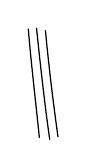
\begin{tikzpicture}[x=1mm,y=1mm,line width=.45pt,line cap=round]
\draw (0,14.0) .. controls (.36,9.6) and (1.02,4.1) .. (1.40,.25);
\draw (1.05,14.1) .. controls (1.53,9.4) and (2.14,4.0) .. (2.72,0);
\draw (2.18,13.8) .. controls (2.62,9.0) and (3.26,4.0) .. (3.77,.32);
\end{tikzpicture}}}
\margin{\uline{NB} \unsure{si|Si} $u,\sigma$ sont des éléments d'un groupe $G$, on pose bien sûr $u(\sigma)=u\sigma u^{-1}$.}
\margin{ceci \uline{implique que}, \deleted{\unsure{par}} $\operatorname{int}(u_{\alpha,\beta,f})$ a même effet, \unsure{sur|en} $\mathrm{Sl}(2,\widehat{\mathbb Z})'$ que l'\unsure{autom} $u$ de $\unsure{\widehat{\mathcal G}_{0,3}^{+}|\widetilde{\mathcal G}_{0,3}^{\to}}$ défini (quand il y en a un), par passage au quotient en $\mathrm{Sl}(2,\widehat{\mathbb Z})'$.}

formules qui se réduisent à des formules où $f$ à nouveau a disparu
\[
(81)\qquad
\left\{\begin{aligned}
u_{\alpha,\beta}(\sigma_\infty)&=\operatorname{int}(\beta)(\sigma_\infty)\\
u_{\alpha,\beta}(\rho)&=\operatorname{int}(\unsure{\alpha|\beta})(\rho)
\end{aligned}\right.,
\]
qui \deleted{à leur tour} résultent \inserted{\uline{trivialement}} des deux expressions \deleted{de} (78) de $u_{\alpha,\beta}$ !

Les formules (80) se complètent de façon naturelle en
\[
(82)\qquad
u_{\alpha,\beta,f}(\varepsilon_0)
=\deleted{\unsure{f\varepsilon_0}}\inserted{\varepsilon}\operatorname{int}(f^{-1})(\varepsilon_0^\mu)
\qquad\deleted{\unsure{(\varepsilon=\varepsilon_2)}}
\]
\[
(\text{où }\varepsilon=\varepsilon_2\in\{\pm1\})
\]
\margin{\figure{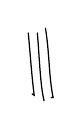
\begin{tikzpicture}[x=1mm,y=1mm,line width=.45pt,line cap=round]
\draw (0,8.6) .. controls (.28,5.5) and (.48,2.7) .. (.75,.7) -- (.48,.86);
\draw (1.15,8.6) .. controls (1.44,5.1) and (1.52,2.0) .. (2.0,0);
\draw (2.18,9.2) .. controls (2.68,6.2) and (2.62,2.9) .. (3.15,.43) -- (2.90,.39);
\end{tikzpicture}}}
qui à son tour se réduit à
\[
(83)\qquad u_{\alpha,\beta}(\varepsilon_0)=\varepsilon.\varepsilon_0^\mu
\]
où $f$ ne figure plus. Comme $\varepsilon_0=\sigma_\infty\rho$, cette formule se réduit à :
\[
u_{\alpha,\beta}(\sigma_\infty)u_{\alpha,\beta}(\rho)=\varepsilon.\varepsilon_0^\mu,
\]
qui compte tenu de (81) se réduit à :
\[
\operatorname{int}(\beta)(\sigma_\infty)\operatorname{int}(\unsure{\alpha|\beta})(\rho)=\varepsilon.\varepsilon_0^\mu
\]
\deleted{\unsure{puis}}
\[
\deleted{\unsure{\alpha\sigma_\infty\alpha^{-1}\beta\rho\beta^{-1}}}
\]
\scanpage{201}

or le premier \unsure{mb} s'écrit
\[
\deleted{\unsure{\beta\sigma_\infty\beta^{-1}\alpha\rho\alpha^{-1}
=(\beta\sigma_\infty\beta^{-1}\sigma_\infty)(\sigma_\infty\rho)(\rho^{-1}\alpha\rho\alpha^{-1})}}
\]
\[
\deleted{\unsure{=(\beta\sigma_\infty(\beta)^{-1})\varepsilon_0(\rho^{-1}(\alpha)\beta^{-1})}}
\]
\[
\begin{aligned}
\beta\sigma_\infty\beta^{-1}\alpha\rho\alpha^{-1}
&=\underbrace{(\beta\sigma_\infty\beta^{-1}\sigma_\infty)}_{\beta\sigma_\infty(\beta)^{-1}}
\underbrace{(\sigma_\infty\rho)}_{\varepsilon_0}
\underbrace{(\rho^{-1}\alpha\rho\alpha^{-1})}_{\rho^{-1}(\alpha)\alpha^{-1}=\rho^{-1}(\alpha\rho(\alpha)^{-1})}\\
&=\eta.\varepsilon_0.\rho^{-1}(\xi)
=\eta.\underbrace{(\varepsilon_0\rho^{-1})}_{\sigma_\infty}(\xi).\varepsilon_0
=\eta\sigma_\infty(\xi)\varepsilon_0
\end{aligned}
\]
donc la relation (83) s'écrit aussi
\[
\eta\sigma_\infty(\xi)=\varepsilon\varepsilon_0^{\mu-1}\quad(=\varepsilon \ell_0^\nu)
\]
or on a $\xi=\varepsilon\eta \ell_1^\nu$ (relation des lacets (60))

donc
\[
\eta\sigma_\infty(\xi)=\varepsilon\eta\sigma_\infty(\eta)\ell_0^\nu=\varepsilon \ell_0^\nu,\quad\text{OK.}
\]

\uline{Remarque.} Toutes ces formules sont valables dans $\mathrm{Gl}(2,\widehat{\mathbb Z})$, sans ambiguïté de signes, dès que $\alpha,\beta,f$ sont choisis. Si on change les signes de $\alpha$ \unsure{ou|et} de $\beta$ ou les deux, la relation des lacets n'est pas modifiée --- et $u_{\alpha,\beta}$ n'est pas \unsure{changé} non plus, \deleted{Par contre} ni $u_{\alpha,\beta,f}$ (si on ne touche pas à $f$). Par contre, un \unsure{chgt.} de signe sur $f$ implique un \unsure{chgt.} de signe sur $u_{\alpha,\beta,f}$. Mais un tel changement de signe ne change bien sûr rien à la validité des formules (80), (82). Quand on fait
\scanpage{202}
\mspage{400}

sur $(\alpha,\beta,f)$ les changements \unsure{les}
\[
(84)\qquad
\alpha'=\ell_0^n\alpha,\qquad\beta'=\ell_0^n\beta,\qquad f'=\ell_0^n f
\qquad(n\in\mathbb Z)
\]
alors \deleted{\illegible{1}}
\[
(85)\qquad
\left\{\begin{aligned}
c'&=\unsure{c},\quad d'=d& t'&=t,\quad u'=u\\
\underbrace{f'^{-1}\alpha'}_{\alpha'_0}&=\underbrace{f^{-1}\alpha}_{\alpha_0}&
\underbrace{f'^{-1}\beta'}_{\beta'_0}&=\underbrace{f^{-1}\beta}_{\beta_0}
\end{aligned}\right.
\qquad\deleted{\unsure{\mu'=\mu|u'=u}}
\]
\deleted{enfin}
\[
\deleted{\unsure{\delta'=\delta}\text{ car}}
\qquad\deleted{\unsure{u_{\alpha',\beta'}}}
\]
enfin
\[
\delta'(=\det\alpha')=\delta(=\det\alpha)\quad(\text{car }\det \ell_0^n=1)
\]
\[
(86)\qquad
\left\{\begin{aligned}
\text{d'où}\quad\deleted{\unsure{f}}\quad
\mu'\bigl(=\delta'/(c'^2+c'd'+d'^2)\bigr)&=\mu\bigl(=\delta/(c^2+cd+d^2)\bigr)\\
\text{d'où}\quad\varepsilon'_2&=\varepsilon_2,\quad\alpha'_2=\alpha_2.
\end{aligned}\right.
\]
c'est le \unsure{double} de ce qu'il faut pour vérifier \inserted{avec (79)} que
\[
(87)\qquad u_{\alpha',\beta',f'}=u_{\alpha,\beta,f}.
\]

Rappelons aussi (cf prop. page 384)

\uline{Proposition.} Soient $\mu\in\widehat{\mathbb Z}^*$, d'où les signes $\varepsilon_2=\varepsilon_2(\mu)$ et $\varepsilon_3=\varepsilon_3(\mu)$ (définis par $\mu\equiv\varepsilon_2\ (4)$, $\mu\equiv\varepsilon_3\ (3)$), et soient $c,d,t,u\in\widehat{\mathbb Z}$. Pour qu'il existe $a,b,r,s\in\widehat{\mathbb Z}$
\[
\alpha=\begin{pmatrix}a&b\\c&d\end{pmatrix},\qquad
\beta=\begin{pmatrix}r&s\\t&u\end{pmatrix}
\quad\text{satisfaisant (64)}
\]
\[
ad-bc=\varepsilon_3\qquad ru-st=1
\]
et la relation des lacets
\[
\alpha\rho(\alpha)^{-1}=\varepsilon_2\bigl(\beta\sigma_\infty(\beta^{-1})\bigr)\ell_1^\nu
\qquad\text{où }\nu=(\mu-1)/2
\]
(i.e les relations (73)) il f. et s. qu'on ait
\[
(88)\qquad\varepsilon_3(c^2+cd+d^2)=\varepsilon_2(t^2+u^2)=1/\mu,
\]
et \unsure{l'ens|l'ens.} des couples $(\alpha,\beta)$ satisfaisant ces conditions est un \uline{torseur} sous $\widehat{\mathbb Z}$, opérant

\margin{\uline{NB} Pour $\mu$ fixé, on peut tjrs trouver $c,d,t,u$ satisfaisant la relation (88) --- heureusement !}
\scanpage{203}

par
\[
 (\alpha,\beta)\longmapsto
 (\unsure{\varepsilon_0^n}\alpha,\varepsilon_0^n\beta).
\]
\deleted{\illegible{1}}

\uline{Corollaire} Pour qu'on puisse trouver $\alpha,\beta$ tels qu'on ait de plus $\alpha\equiv\beta\equiv1\ (2)$, il f. et s. qu'on ait
\[
\tag{89}
 c\equiv t\equiv0\ (2)\qquad d\equiv u\equiv\unsure{1}\ (2),
\]
et alors \unsure{l'ens.} des solutions $(\alpha,\beta)$ satisfaisant à ces conditions supplémentaires est un torseur sous $\widehat{\mathbb Z}$, opérant par
\[
 (\alpha,\beta)\longmapsto(\ell_0^n\alpha,\ell_0^n\beta).
\]

\uline{Scholie} On peut donc dire que pour un élément \inserted{$u$} de $\mathcal N_{0,3}^{!\sim}$, qui définit \unsure{donc|deux} $\alpha,\beta$ dans $\Pi_{0,3}^{\sim\wedge},\Pi_{0,3}^{\wedge}$ \inserted{(\uline{modulo} les \unsure{transformations} $(\alpha,\beta)\mapsto(\ell_0^n\alpha,\ell_0^n\beta)$),} (satisfaisant la relation des lacets), il lui est attaché les ``invariants adéliques'' \deleted{\illegible{3}}
\[
\tag{90}
 \Theta=(\mu,c,d,t,u)
\]
($c,d,t,u$ déterminés aux \unsure{\uline{ambiguïtés}|ambiguïtés} de signes, sans plus) satisfaisant (88) --- et c'est \uline{ce qu'on peut faire de mieux} dans le contexte actuel : les $a,b,r,s$ \unsure{n'ont|n'est} pas un caractère invariant. Quand on a un élément \inserted{$\underline u$} de $\unsure{\mathcal M_{0,3}^{!\sim}|\mathcal N_{0,3}^{!\sim}}$ --- i.e. un automorphisme \unsure{effectif}, pas seulement ext. --- on a de plus un $\underline f\in\Pi_{0,3}^{\wedge}$, donnant un $f\in\mathrm{Sl}(2,\widehat{\mathbb Z})'$, d'où
\[
\tag{91}
 f=\begin{pmatrix}\unsure{j}&\unsure{k}\\ \ell&m\end{pmatrix}
 \qquad\begin{gathered}\uline{\text{défini mod signes}}\\
 \text{et mod } f\longmapsto\ell_0^n f
 \end{gathered}
\]
\scanpage{204}
\mspage{401}

\deleted{d'où \unsure{donc} on}

Mais cette donnée supplémentaire est un peu trop
\deleted{$u_{\alpha,\beta,f}=u_{\mu,c,d,t,u}$}
faible pour reconstituer \deleted{$u_{\alpha,\beta,f}$} l'élément
\[
 \uuline{u}\inserted{{}=\varphi(\underline u)}\deleted{\unsure{\mathrm{d\acute{e}f}}}
 =u_{\alpha,\beta,f}
\]
de $\mathrm{Gl}(2,\widehat{\mathbb Z})'$ associé à $u$.

Il vaut mieux dire que pour $\mu,c,d,t,u$ fixés on a un $\widehat{\mathbb Z}$-torseur de $(\alpha,\beta)\equiv(1,1)\ (2)$ satisfaisant aux conditions dites \unsure{dans|de} la proposition \unsure{§|,} et son corollaire, soit $T=T_\Theta$, on fait opérer alors $\widehat{\mathbb Z}$ \unsure{diagonalement} sur $T\times\mathrm{Sl}(2,\widehat{\mathbb Z})$ par
\[
 (\alpha,\beta,f)\longmapsto
 (\ell_0^n\alpha,\ell_0^n\beta,\ell_0^n f)
\]
et on regarde le quotient --- c'est donc le tordu par $\check T$ (torseur opposé à $T$) de $\mathrm{Sl}(2,\widehat{\mathbb Z})$, sur lequel $\widehat{\mathbb Z}$ opère par $f\longmapsto\ell_0^n f$. \deleted{Il faut} c'est la donnée d'un élément \inserted{$f$} de
\[
 \check T_\Theta\unsure{\mathbin{\wedge}_{\widehat{\mathbb Z}}}\mathrm{Sl}(2,\widehat{\mathbb Z})
 \deleted{\unsure{=\mathcal G_\Theta}}
\]
\margin{c'est un $\mathrm{Sl}(2,\widehat{\mathbb Z})$-torseur à \uuline{droite}}
qui permet de définir un élément
\[
 \uuline{u}=u_{\alpha,\beta,f},
\]
qui change de signe si $f$ est remplacé par $(f(-1))$.

Décidément, ces formulations ne sont pas enthousiasmantes, et il devient clair qu'il faudra introduire explicite-
\scanpage{205}

ment et étudier \deleted{de façon}\inserted{\unsure{avec}} un minimum de soin le \uline{groupe adélique} formé par les systèmes $(\alpha,\beta,f)$ satisfaisant la relation des lacets, et \deleted{\unsure{envisager}} l'homomorphisme canonique de $\mathcal M_{0,3}^{!\sim}$ dans ledit groupe.

Mais je voudrais avant cela terminer les gammes notationnelles.

\deleted{\illegible{1}}
\scanpage{206}
\mspage{402}

\uline{$\overline{\mathrm{IV}}$} Les trois cas particuliers fondamentaux.

On revient aux éléments $g,h,f$ etc \uline{dans} $\Pi_{0,3}^{\wedge}$ et $\Pi_{0,3}^{\sim\wedge}$ qui correspondent à $u$, pouvant être \unsure{décrit|décrits} de quatre façons différentes, par l'un ou l'autre des quatre systèmes
\[
\tag{92}
 (g,h,f),\quad(\alpha_0,\beta_0,f),\quad(\alpha,\beta,f),\quad(\xi,\eta,f).
\]

\inserted{\unsure{$1^\circ$|$1^{\mathrm{er}}$}\ \uline{Cas} :}
\deleted{\illegible{1}\ \uline{Cas}\ \illegible{1}}
\[
\tag{93}
 h=1,\quad\text{i.e. }\beta_0=1,\quad\text{i.e. }\beta=f,\quad
 \text{i.e. }\eta=f\sigma_\infty(f)^{-1},
\]
i.e.
\[
\tag{94}
 [u,\sigma_\infty]=1.
\]

Pour un $u$ \inserted{\uline{quelconque}} \unsure{(}i.e. un système $(g,h,f)$ etc quelconque, il y a un \unsure{autom.} intérieur et un seul $\operatorname{int}(\gamma)$ tel que \inserted{$u'=\operatorname{int}(\gamma)\unsure{u}$} \unsure{satisfasse} à la propriété précédente i.e. commute à $\sigma_\infty$, \deleted{\illegible{1}} ce sera pour
\[
 \gamma=\beta_0^{-1}\qquad(\text{cf formules (49)}).
\]
\deleted{\illegible{1}}

Les $u$ satisfaisant à (93), exprimés en termes de triplets $(\xi,\eta,f)$ satisfaisant les trois relations (44) (46) (ne faisant pas intervenir $f$), \deleted{\illegible{1}} correspondent ainsi (par la relation $\eta=f\sigma_\infty(f)^{-1}$ de (93)) aux \deleted{\unsure{triplets}} couples $(\xi,f)$ d'éléments de $\Pi_{0,3}^{\wedge}$, satisfaisant
\[
\tag{95}
 \xi\,\rho(\xi)\,\rho^2(\xi)=1
\]
\[
\tag{96}
 \xi=(f\sigma_\infty(f)^{-1})\ell_1^\nu
\]
\inserted{avec $\nu\in\widehat{\mathbb Z}$, comme \unsure{variable}, tel que $2\nu+1\in\widehat{\mathbb Z}^{*}$}

\margin{\uline{NB} \unsure{on aura}
$\xi=fg\rho(f)^{-1}$.
\unsure{au lieu de} $f$ \unsure{il est licite|il est légitime} \unsure{d'écrire} \unsure{ici} $\unsure{\beta}$ --- \unsure{mais alors} \illegible{2} $\unsure{\beta}$ \unsure{déterminés} \unsure{par} \illegible{2} $\unsure{\ell_0^n}$ \illegible{2} $\unsure{f\longmapsto\ell_0^n f}$ \illegible{2}}
% ===== LM_C3-207-225: second pass, checked against the scans =====
\scanpage{207}

ou aux couples $(\alpha,\beta)$ d'éléments de $\widehat{\Pi}_{0,3}$
satisfaisant la relation des lacets (37)
\[
 (97)=(37)\qquad
 \unsure{(\alpha\rho(\alpha)^{-1})}
 =(\beta\sigma_\infty(\beta)^{-1})\ell_1^{\unsure{\nu}}
\]
(qu'on complètera alors en prenant $f=\beta$).

\margin{$\alpha,\beta$ \unsure{déterminés} \unsure{mod}
$(\alpha,\beta)\longmapsto
(\ell_0^{\unsure{n}}\alpha,\ell_0^{\unsure{n}}\beta)$.}

Au changement près de $\alpha$ en $\ell_0^\nu\alpha=\underline{\alpha}_0$,
c'étaient les conventions du \unsure{§ 44|§ 4 h} (où la formule prend
\unsure{donc} la forme
\[
 \underbrace{\underline{\alpha}_0\rho(\underline{\alpha}_0)^{-1}}_{\xi}
 =\ell_0^\nu
 \underbrace{(f\sigma_\infty(f)^{-1})}_{\unsure{\varphi=\eta}}
\]
\unsure{).}

Compte tenu de (79), les conditions

\deleted{\uline{2° Cas}
\unsure{(98)} $g=1$ i.e. $\unsure{\alpha_0}=1$ i.e. $f=\alpha$,
i.e. $\xi=f\rho(f)^{-1}$ i.e.}

(93) (94) prennent aussi la forme
\[
 (98)\qquad u_{\alpha,\beta,f}
 =\mu(t\sigma_\infty+u)\tau_\infty^{\alpha_2},
\]
et impliquent que $\underline{u}=u_{\alpha,\beta,f}$
\deleted{\illegible{1}} normalise la sous-algèbre de l'algèbre des matrices
$M_2(\widehat{\mathbb Z})$ \uline{engendrée} par $\sigma_\infty$
(compte tenu de la relation
\[
 (99)\qquad \tau_\infty(\sigma_\infty)=-\sigma_\infty
 \qquad\text{dans }\mathrm{Gl}(2,\widehat{\mathbb Z}).
\]

Si on regarde le sous-groupe de $\mathcal M_{0,3}^{!\sim}$
formé des $u$ qui satisfont aux conditions équivalentes (93) (94) (98)
\[
 (100)\qquad
 \mathcal M_{0,3}^{!\sim}\left(\tfrac12\right)
 =
 \{u\in\mathcal M_{0,3}^{!\sim}\mid [u,\sigma_\infty]=1\}
 \overset{\sim}{\longrightarrow}\mathcal N_{0,3}^{!\sim}
\]
on trouve que l'hom composé
\scanpage{208}
\mspage{403}

(101)
\diagram{
\begin{tikzcd}[ampersand replacement=\&,column sep=large]
\mathcal N_{0,3}^{!\sim}
 \arrow[r,"\sim"]
 \arrow[rr,bend right=22,"k_{1/2}"']
\&
\mathcal M_{0,3}^{!}(\tfrac12)^\sim
 \arrow[r]
\&
\mathcal M_{0,3}^{!\sim}
 \arrow[r,"{u\longmapsto\underline{u}=(u_{\alpha,\beta,f})}"']
\&
\mathrm{Gl}(2,\widehat{\mathbb Z})'
\\
\unsure{\mathcal N_{0,3}^{!\sim}(\tfrac12)}
\end{tikzcd}
}

\margin{\uline{NB} $\mathcal M_{0,3}^{!}(\tfrac12)^\sim$
est stable par $x\longmapsto\sigma_\infty x\sigma_\infty^{-1}$
et par $x\longmapsto\tau_\infty x\tau_\infty^{-1}$
(puisque $\sigma_\infty$ et $\tau_\infty$
\unsure{commutent} à $\sigma_\infty$).}

factorise par le dit normalisateur --- si on préfère le voir en termes du
groupe $\mathrm{Gl}(2,\widehat{\mathbb Z})\simeq M_2(\widehat{\mathbb Z})^*$,
plutôt que de l'\uline{algèbre} des matrices, elle se factorise par
le \uline{normalisateur} du \uline{tore maximal}
\deleted{(\unsure{formé par})}
\[
 (102)\qquad
 \unsure{T_\alpha|T_\sigma}=
 \{t\sigma_\infty+u\quad
 (t,u\in\unsure{\widehat{\mathbb Z}|\mathbb Z},
 \underbrace{t^2+u^2}_{=\det(t\sigma_\infty+u)}
 \in\widehat{\mathbb Z}^{*}).
\]

Je suspecte qu'il n'y a \uline{que le} scindage $k_{1/2}$ de (101)
de l'extension $\mathcal M_{0,3}^{!\sim}$
(de $\mathcal N_{0,3}^{!\sim}$ par $\widehat{\Pi}_{0,3}$,
\deleted{\unsure{Je crois}} ou de $\mathcal N_{0,3}^{!\sim}$
par $\widehat{\mathcal G}_{0,3}^{+}$)
qui se factorise par le normalisateur.

\margin{Sûrement canulé :
il y a aussi \unsure{toutes} les courbes \uuline{\unsure{isogènes}}
à la courbe elliptique d'invariant modulaire $\unsure{j|J}=0$
(\unsure{correspondant} \deleted{dans}
l'orbite $\{\tfrac12,2,-1\}$ dans $U_{0,3}$ sous $\unsure{\mathfrak S_3}$).}

\uline{2° Cas}\quad C'est le cas
\[
 (103)\qquad
 g=1\quad\text{i.e. }\unsure{\alpha_0}=1
 \quad\text{i.e. }\alpha=f
 \quad\text{i.e. }\xi=f\rho(f)^{-1},\ \text{i.e.}
\]
\[
 (104)\qquad [u,\rho]=1.
\]

Pour un $u$ quelconque, il y a un
$\gamma\inserted{\in\widetilde{\widehat{\Pi}}_{0,3}
=\widehat{\Pi}_{0,3}\cdot\{1,\tau_\infty\}}$
\deleted{\unsure{unique}} tel que
$u'=\mathrm{int}(\gamma)\circ u=\gamma u$
\unsure{commute|commutant} ainsi à $\rho$,
savoir $\gamma=\unsure{\alpha_0^{-1}}$,
\deleted{\unsure{On a donc}}\inserted{Mais} on fera Attention que
$\gamma$ n'est pas toujours dans $\widehat{\Pi}_{0,3}$, en fait
\[
 (105)\qquad
 \gamma=\unsure{\alpha_0^{-1}}\in\widehat{\Pi}_{0,3}
 \Longleftrightarrow
 \varepsilon_3(\unsure{u})=1
 \quad\text{i.e. }\mu(u)=1\ (3)
\]
\scanpage{209}

Si on désigne par
$\unsure{\mathcal M_{0,3}^{!\sim}}(\unsure{-\overline{j}})$
le sous-groupe de $\mathcal M_{0,3}^{!\sim}$
formé des $u$ satisfaisant (103), (104), son image dans
$\unsure{\mathcal N_{0,3}^{!\sim}}$ est donc
le sous-groupe d'indice $2$ noyau de
\[
 u\longmapsto
 \underbrace{\varepsilon_3(\mu(u))}_{\unsure{\sim}}
 =\varepsilon_3(u)
\]
i.e.
\[
 \unsure{(106)}\qquad
 \mathcal N_{0,3}^{!\sim}(-\overline{j})
 =\{u\in\mathcal N_{0,3}^{!\sim}\mid
 \varepsilon_3(u)=1\quad
 \text{i.e. }\mu(u)\equiv1\ (3)\}
\]

\margin{\uline{NB} $\mathcal M_{0,3}^{!\sim}(-\overline{j})$
est stable par $x\longmapsto\rho x\rho^{-1}$.}

et l'on a
\[
 \unsure{(107)}\qquad
 \unsure{\mathcal M_{0,3}^{!\sim}}[-\overline{j}]
 \overset{\sim}{\longrightarrow}
 \mathcal N_{0,3}^{!\sim}[-\overline{j}].
\]

En l'inversant on trouve donc un
\deleted{hom composé}\inserted{scindage}

(108)
\diagram{
\begin{tikzcd}[ampersand replacement=\&,column sep=large]
\mathcal N_{0,3}^{!\sim}(\unsure{-\overline{j}})
 \arrow[r,"\sim"]
 \arrow[rr,bend right=20,"{k(-\overline{j})}"']
\&
\mathcal M_{0,3}^{!\sim}(\unsure{-\overline{j}})
 \arrow[r,hook]
\&
\mathcal M_{0,3}^{!\sim}
\end{tikzcd}
}
,
dont le composé avec $\mathcal M_{0,3}^{!\sim}$ est un hom qui
\deleted{\unsure{factorise}}\inserted{se factorise}
par le tore maximal $T_\rho$ de $\mathrm{Gl}(2,\widehat{\mathbb Z})'$,
formé des
\deleted{$\unsure{c\rho+d}$}
\[
 \unsure{(109)}\qquad
 \{c\rho+d\mid c,d\in\widehat{\mathbb Z},\
 c^2+cd+d^2\in\widehat{\mathbb Z}^{*}).
\]

Je suspecte que c'est le seul scindage de
$\mathcal M_{0,3}^{!\sim}$
(ou \unsure{$\overline{\mathrm m}$} de $\mathcal M_{0,3}^{!}$)
qui ait cette propriété. \unsure{Celle-ci} résulte de la forme équivalente
des conditions (103) (104), fournie par (79) :

\margin{\unsure{canulé}, pour \unsure{mêmes} raisons que tout à l'heure\ldots}
\scanpage{210}
\mspage{404}

\[
 (110)\qquad
 \underline{u}=u_{\alpha,\beta,f}=\mu(c\rho+d)
\]
(NB $\delta=\varepsilon_3(\unsure{\mu|u})$ est égal à $1$ dans ce cas).

Les $u$ en question correspondent aux couples $(\eta,f)$ satisfaisant
\[
 (111)\qquad \eta\sigma_\infty(\eta)=1
\]
\[
 \unsure{(112)}\qquad
 (f\rho(f)^{-1})=\eta\ell_1^{\unsure{\nu}}
\]

\margin{qu'on \unsure{complètera|complète} par $\xi=f\rho(f)^{-1}$.}

\margin{On peut aussi écrire $\beta$ au lieu de \unsure{$f$},
$f(=\beta)$ \unsure{déterminé} mod
$f\longmapsto\ell_0^{\unsure{n}}f$,
\unsure{id.} pour $\alpha,\beta$.}

ou encore aux couples $(\alpha,\beta)$ satisfaisant la relation des lacets
$(97)=(37)$, qu'on complète alors par $f=\alpha$.

\uline{3° Cas}\quad C'est celui où
\[
 (113)\qquad
 f\equiv1\ (L_0)
 \quad\text{i.e. }\alpha\equiv\alpha_0\ (L_0\text{ à g.})
 \quad\text{i.e. }\beta\equiv\beta_0\ (L_0\text{ à g.})
\]
ou encore $u(\varepsilon_0)=\varepsilon_0^\mu$
$(\mu\in\widehat{\mathbb Z}^{*})$ i.e.
\[
 (114)\qquad
 [u,\varepsilon_0]=\ell_0^\nu
 \qquad
 (\nu\in\widehat{\mathbb Z}\ -\ \nu=\tfrac{\mu-1}{2}),
\]
\inserted{i.e. $u$ normalise
$L_0=\{\ell_0^n\mid n\in\widehat{\mathbb Z}\}$ --- ou encore
(\unsure{agrandissant} $\widehat{\Pi}_{0,3}$)
$u$ normalise $L'_0=\{\varepsilon_0^n\mid n\in\widehat{\mathbb Z}\}$.}

\margin{\uline{NB} $L_0=L'_0\cap\widehat{\Pi}_{0,3}$.}

Dans ce cas, on \unsure{lève|peut lever} l'indétermination
$(\alpha,\beta,f)\longmapsto
(\ell_0^n\alpha,\ell_0^n\beta,\ell_0^n f)$
en exigeant
\[
 (115)\qquad f=1,
\]
ce qui détermine $\alpha,\beta$ de façon unique.

\deleted{L'ensemble}\inserted{groupe}
$\mathcal M_{0,3}^{!\sim}[0]$ des $u\in\mathcal M_{0,3}^{!\sim}$
qui normalisent $L_0$ est en corr. biunivoque avec l'ens des couples
$(\alpha,\beta)$
$(\alpha\in\widetilde{\widehat{\Pi}}_{0,3}
=\widehat{\Pi}_{0,3}\cdot\{1,\tau_\infty\},
\ \beta\in\widehat{\Pi}_{0,3})$ satisfaisant

\margin{On ne \unsure{remonte|relève} Donc \illegible{2}
par $\mathcal M_{0,3}^{!\sim}(0)$,
\illegible{2} $\mathcal M_{0,3}$ et $\mathcal N_{0,3}$
car il \unsure{ne couvre} \illegible{2}
section de l'ext. \illegible{2} par $\widehat{\Pi}_{0,3}$
--- on \illegible{2} (Prop. \illegible{1})
section $\mathcal M_{0,3}^{!\sim}(0)$ plus
\unsure{p. 412$^1$}).}
\scanpage{211}

la sempiternelle relation des lacets
\[
 \unsure{(115)}\qquad
 (\alpha\rho(\alpha)^{-1})
 =(\beta\sigma_\infty(\beta)^{-1})\ell_1^\nu
 \qquad(\text{pour }\nu\in\widehat{\mathbb Z}\text{ conv.})
\]
\inserted{(par $(\alpha,\beta)\longmapsto
\unsure{g|\xi}=\alpha\rho(\alpha)^{-1};
\unsure{h|\eta}=\beta\sigma_\infty(\beta)^{-1}$)}
ou encore aux couples $(g,h)$
\inserted{(\unsure{ou} $(\xi,\eta)$)}
d'éléments de $\widehat{\Pi}_{0,3}$ satisfaisant
\[
 \begin{gathered}
 (116)\quad (=(44)+(46))\\
 g\rho(g)\rho^2(g)=1,\qquad
 \unsure{h}\sigma_\infty(\unsure{h})=1,\qquad
 g=\unsure{h}\ell_1^\nu\quad
 (\nu\in\widehat{\mathbb Z}\text{ conv.}),
 \end{gathered}
\]

\margin{Dans tout ceci, je laisse tomber la "condition
liminaire" sur les relations génératrices\ldots}

au couple \deleted{$(\alpha,\beta)$ \unsure{comme}}
$(g,h)$ correspond l'automorphisme $u$ défini par
\[
 (117)=(23)\qquad
 u(\sigma_\infty)=\unsure{h}\sigma_\infty,\qquad
 u(\rho)=g\rho
\]
ou encore par
\[
 (118)\qquad
 \unsure{u}(\sigma_\infty)=\mathrm{int}(\alpha)\sigma_\infty,\qquad
 u(\rho)=\mathrm{int}(\beta)\rho.
\]

Dans le groupe $\mathcal M_{0,3}^{!\sim}[0]$, il y a le sous groupe
\[
 (119)\qquad
 \mathcal M_{0,3}^{!\sim}[0]\cap\widehat{\Pi}_{0,3}\simeq L_0
\]
l'inclusion
\[
 (120)\qquad
 \widehat{\mathbb Z}\overset{\ell_0}{\underset{\sim}{\longrightarrow}}
 L_0\lhook\joinrel\longrightarrow\mathcal M_{0,3}^{!\sim}
\]
étant décrite par
\[
 (121)\qquad
 \lambda=\ell_0^n\longmapsto
 (\alpha=\unsure{\lambda|\ell_0^n},
 \beta=\unsure{\lambda|\ell_0^n})
\]
\deleted{\unsure{i.e.}\ \illegible{2}\ $(\alpha=\lambda,\beta=$}

ou encore par
\[
 (122)\qquad
 \lambda=\ell_0^{\unsure{n}}\longmapsto
 (f=\ell_0^n\ell_1^{-n},g=\ell_0^n\ell_1^{-n})
\]
\inserted{i.e. $f=g=\lambda\sigma_\infty(\unsure{\lambda^{-1}})
=\lambda\rho(\unsure{\lambda})^{-1}$,}
la multiplication \deleted{par} à g. par \unsure{le}
$\lambda=\ell_0^n$ dans $\mathcal M_{0,3}^{!\sim}[0]$
étant \unsure{explicité|explicitée} par
\[
 (123)\qquad
 (\alpha,\beta)\longmapsto(\ell_0^n\alpha,\ell_0^n\beta)
\]
\[
 (124)\qquad
 (\xi,\eta)\longmapsto
 \ell_0^n\xi\ell_1^{-n},\ \ell_0^n\eta\ell_1^{-n}).
\]
\scanpage{212}
\mspage{405}

Comme on a un iso
\[
\mathcal M_{0,3}^{!\sim}[0]/L_0
\xrightarrow{\sim}\mathcal N_{0,3}^{!\sim},
\]
on trouve le

\uline{Corollaire} Le groupe $\mathcal N_{0,3}^{!\sim}$ est en bijection
canonique avec l'ens des couples
$(\alpha,\beta)\in\Pi_{0,3}^{\sim\wedge}\times\Pi_{0,3}^{\wedge}$
satisfaisant la relation des lacets (97)
\[
\alpha\rho(\alpha)^{-1}
=\bigl(\beta\sigma_\infty(\beta)^{-1}\bigr)\ell_1^\nu
\qquad(\text{pour }\nu\in\widehat{\mathbb Z}\text{ conv.}),
\]
\uline{modulo} les transformations
$(\alpha,\beta)\mapsto(\ell_0^{\unsure{n|m}}\alpha,\ell_0^{\unsure{n|m}}\beta)$.

La loi de groupe \inserted{(de $\mathcal M_{0,3}^{!\sim}(0)$ ou de son quotient
$\mathcal N_{0,3}^{!\sim}$)} s'explicite en termes des $(g,h)$, ou des
$(\alpha,\beta)$, par les ``formules des cocycles'' (52) : si $u',u$
\inserted{et $u''=u'\cdot u$} sont donnés par
$\unsure{(g',h')},(g,h),(g'',h'')$, ou par
$(\alpha',\beta'),(\alpha,\beta)$ et $(\alpha'',\beta'')$, on aura
\[
\tag{125}
\left\{
\begin{aligned}
g''&=u'(g)g'&h''&=u'(h)h'\\
\alpha''&=u'(\alpha)\alpha'&\beta''&=u'(\beta)\beta'.
\end{aligned}
\right.
\]

\uline{Remarque sur les notations} $\mathcal M_{0,3}^{!\sim}(q)$,
pour $q=\frac12,-\overline j,0$.
En fait pour tout point \uline{algébrique}
\[
\tag{126}
q\in\mathcal U_{0,3}(\mathbb C)
=\mathbb C\setminus\{0,1\}
=\mathbb P^1_{\unsure{\mathbb C|\mathbb Q}}(\mathbb C)
\setminus\{0,1,\infty\}
\]
on s'attend à \deleted{\unsure{trouver}} un scind. partiel
\[
\tag{127}
k_q:\unsure{\mathcal N|\mathcal M}_{0,3}^{!\sim}(q)\longrightarrow\mathcal M_{0,3}^{!\sim},
\qquad\operatorname{Im}k_q\overset{\text{déf}}=\mathcal M_{0,3}^{!\sim}(q)
\]
de l'extension $\mathcal M_{0,3}^{!\sim}$ de
$\mathcal N_{0,3}^{!\sim}$ par $\Pi_{0,3}^{\wedge}$, ou

\margin{En fait, \unsure{de façon} \illegible{1} plus
\unsure{précise|précises}, $k_q$ ne sera \unsure{déterminé}
qu'à \unsure{autom.} int. près...}
\scanpage{213}

du moins \inserted{on aura} un scindage partiel au dessus
de $\Gamma_{\mathbb Q}(q)$, qu'on s'efforcera de déterminer ;
$\mathcal N_{0,3}^{!\sim}(q)$ désigne un sous-groupe
hypothétique de $\mathcal N_{0,3}^{!\sim}$
(qu'il faudrait \unsure{arriver} à déterminer, \unsure{si tant est}
\illegible{1} pas trop \illegible{1}...), induisant sur $\Gamma_{\mathbb Q}$
le sous-groupe \inserted{ouvert} $\Gamma_{\mathbb Q}(q)$ de
$\Gamma_{\mathbb Q}$ stabilisateur de $q$.

\margin{La définition s'impose p.ex. lorsque $q$ est
\unsure{élément} d'une extension cyclotomique de $\mathbb Q$, de telle
façon que $\mathbb Q(q)$ correspond à un groupe quotient fini
discret de $\widehat{\mathbb Z}^{*}$ et $\Gamma_{\mathbb Q}(q)$ est
le noyau de
\diagram{\begin{tikzcd}[ampersand replacement=\&]
\Gamma_{\mathbb Q}\arrow[r,"\chi"]\&\widehat{\mathbb Z}^{*}\arrow[r]\&G
\end{tikzcd}}\ldots}

L'analyse des cas $1^\circ$ et $2^\circ$ ci-dessus revenait en fait à
la détermination de tels scindages, pour $q=\frac12$ et pour
$q=-\overline j$ --- dans le premier cas $\Gamma_{\mathbb Q}(q)$ est
$\Gamma_{\mathbb Q}$ tout entier, dans le deuxième c'est le sous-groupe
d'indice $2$ noyau de $\varepsilon_2\circ\chi:\Gamma_{\mathbb Q}
\longrightarrow\{\pm1\}$, et idem pour
$\unsure{\mathcal N|\mathcal M}_{0,3}^{!\sim}(q)$.
En transformant par $\rho$ \inserted{et $\rho^2$}, on
\deleted{\unsure{conduirait}}\inserted{déduirait} \unsure{des scindages|du scindage} $k_{1/2}$
les scindages $k_2$ et $k_{-1}$ --- en transformant par un quelconque
des $\sigma_{\unsure{i|\rho}}$,
\deleted{ou par un des $\unsure{\tau_i|\sigma_i}$}, on déduirait
du scindage $k_{-\overline j}$ un scindage du type $k_{\unsure{-j|-1}}$.

Quant à $\mathcal M_{0,3}^{!\sim}[0]$, il correspond
\inserted{en principe} au point
\scanpage{214}
\mspage{406}

$0$ de $\widehat{\mathcal U}_{0,3}=\unsure{\mathbb P^1_{\mathbb Q}}$,
il \deleted{\unsure{y correspondent par}}\inserted{deux autres}
sous-groupes analogues $\mathcal M_{0,3}^{!\sim}[q]$, avec
$q=1$, $q=\infty$, correspondant aux deux autres points ``à l'infini''
de $\mathcal U_{0,3}$, et qui se déduisent du précédent en appliquant
$\rho$, $\rho^2$.
Ici, on a des groupes qui \uline{ne} correspondent \uline{pas}
\inserted{\unsure{strictement}} à des sections \inserted{même} partielles
de $\mathcal M_{0,3}^{!\sim}$ sur $\mathcal N_{0,3}^{!\sim}$,
puisque l'intersection avec $\Pi_{0,3}^{\wedge}$ n'est pas réduite à $1$,
mais c'est l'un des trois groupes-lacets type $L_0,L_1,L_\infty$.

Mais on sait que \inserted{le choix d'}un \unsure{uniformisant|uniformisante}
de l'anneau local de $\widehat{\mathcal U}_{0,3}$ en $0$ (disons)
détermine un scindage de
$\mathcal M_{0,3}^{!\unsure{\sim}}\unsure{(0)|[0]}$, considéré comme
ext. de $\mathcal N_{0,3}^{!}$ par $L_0$ --- et il faudra
dans la suite essayer de saisir \deleted{\unsure{ce}}\inserted{un tel}
scindage \inserted{(associé à une \unsure{uniformisante})}
dans l'optique de notre calcul, comme une façon \unsure{privilégiée}
\deleted{de ``\unsure{normaliser}''}, pour \unsure{tte}
\deleted{$\alpha,\beta$} \unsure{donnée} \inserted{mod $L_0$} de $(\alpha,\beta)$
satisfaisant une relation des lacets, de ``normaliser'' le choix des
$(\alpha,\beta)$ mod $L_0$.
J'y reviendrai par la suite, sûrement.
\scanpage{215}
\mspage{407}

\uline{V} \uline{Récapitulation} \uline{en termes de}
$\mathcal M_{0,3}^{!\sim}[0]$

Il apparaît finalement que la façon la plus simple d'étudier les autom.
à lacets de $\Pi_{0,3}^{\wedge}$ (commutant ext.\textsuperscript{t}
à $\mathfrak S_3$, i.e. les éléments de \deleted{\illegible{1}}
$\mathcal N_{0,3}^{!\unsure{\sim}}$) est de commencer par l'étude du
sous-groupe $\mathcal M_{0,3}^{!\unsure{\sim}}[0]$, normalisateur
de $L_0$ \inserted{dans $\mathcal M_{0,3}^{!\sim}$}.
Posant pour $u\in\mathcal M_{0,3}^{!\unsure{\sim}}[0]$
\[
\tag{128}
u(\sigma_\infty)=\eta\sigma_\infty,
\qquad u(\rho)=\xi\rho
\qquad(\eta,\xi\in\Pi_{0,3}^{\wedge})
\]
i.e.
\[
\tag{129}
[u,\sigma_\infty]=\eta\qquad [u,\rho]=\xi
\]
qui expriment la commutation ext. de $u$ à $\mathfrak S_3$
(engendré en effet par $\sigma_\infty$ et $\rho$), la condition de
normalisation de $L_0$ s'exprime par une relation de forme
\[
\tag{130}
u(\varepsilon_0)=\varepsilon_0^\mu
\quad\text{ou}\quad \unsure{u}(\ell_0)=\ell_0^\mu
\qquad(\mu\in\widehat{\mathbb Z}^{*}).
\]

\margin{(130) équivaut aussi, moyennant $[u,\rho]=\xi$, à
\[
\tag{130bis}
\left\{
\begin{aligned}
u(\varepsilon_1)&=\operatorname{int}(\xi)(\varepsilon_1^\mu)\\
&\text{et à}\\
u(\varepsilon_\infty)&=
\operatorname{int}\bigl(\rho^{-1}(\xi^{-1})\,\illegible{1}\bigr)(\varepsilon_\infty^\mu)
\end{aligned}
\right.
\]}

\inserted{Or on a, comme $\varepsilon_0=\sigma_\infty\rho$}
\deleted{qui, compte tenu de $\varepsilon_0=\sigma_\infty\rho$,
prend (par un calcul immédiat) la forme}
\deleted{\unsure{s'écrit}}
\deleted{(131)} \deleted{$\unsure{\eta\sigma_\infty}$}
\[
u(\varepsilon_0)=u(\sigma_\infty)u(\rho)
=\eta\sigma_\infty\xi\rho
=\eta\sigma_\infty(\xi)\underbrace{\sigma_\infty\rho}_{\varepsilon_0}
=\eta\sigma_\infty(\xi)\varepsilon_0
\]
donc (130) s'écrit
\[
\eta\sigma_\infty(\xi)=\varepsilon_0^{\mu-1}
\qquad\text{soit, en posant }\mu-1=2\nu
\quad(\nu\in\widehat{\mathbb Z})
\]
\[
\eta\sigma_\infty(\xi)=\ell_0^\nu
\qquad\text{soit, appliquant }\sigma_\infty
\]
\[
\tag{131}
\sigma_\infty(\eta)\xi=\ell_1^\nu.
\]
Or les relations
\[
\tag{132}
(\eta\sigma_\infty)^2=1,\qquad(\xi\rho)^3=1
\]
s'écrivent aussi
\[
\tag{133}
\boxed{\eta\sigma_\infty(\eta)=1,\qquad
\xi\rho(\xi)\rho^2(\xi)=1},
\]
d'où $\sigma_\infty(\eta)=\eta^{-1}$, de sorte que (131) s'écrit
aussi de façon plus \uline{commode}
\[
\tag{134}
\boxed{\xi=\eta\ell_1^\nu}
\qquad(\text{relation des lacets})
\]
\scanpage{216}

On trouve ainsi le

\uline{Théorème} Les éléments $u$ de
$\unsure{\mathcal M|\mathcal N}_{0,3}^{!\sim}[0]$ --- i.e. les
autom. ext. de $\Pi_{0,3}^{\wedge}$ qui commutent ext.\textsuperscript{t}
à $\mathfrak S_3$ et qui normalisent $L_0$ --- sont en corr.
biunivoque \inserted{(via les formules (128) ou 129)}
avec les couples $(\xi,\eta)$ $(\xi,\eta\in\Pi_{0,3}^{\wedge})$,
satisfaisant les relations (133)(134), et tels que
\inserted{de plus (``condition liminaire'')}
les relations (132) (équivalentes : (133)) soient
\deleted{\unsure{primitives}}\inserted{génératrices}
pour $\widehat{\mathcal G}_{0,3}^{+}$.
(\deleted{\illegible{1}} Dans (134) $\nu$ est un élément convenable de
$\widehat{\mathbb Z}$, évidemment uniquement déterminé, et assujetti
à la condition supplémentaire $2\nu+1\in\widehat{\mathbb Z}^{*}$)
(qui est impliquée par la condition liminaire, et peut-être l'implique...)

\margin{cette condition $2\nu+1\in\widehat{\mathbb Z}^{*}$ est en fait
conséquence des équations (133), (134), cf plus bas th. p. 409!}

\unsure{Et} l'inclusion évidente
\[
\tag{135}
\begin{aligned}
L_0&\hookrightarrow\mathcal M_{0,3}^{!\unsure{\sim}}\unsure{(0)|(\omega)}\\
\ell_0^n=\lambda&\longmapsto\operatorname{int}(\lambda)
\end{aligned}
\]
est donnée par
\[
\tag{136}
\ell_0^n=\lambda\longmapsto
\bigl(\xi=\lambda\rho(\lambda)^{-1}=\ell_0^n\ell_1^{-n},
\quad\eta=\lambda\sigma_\infty(\lambda)^{-1}=\ell_0^n\ell_1^{-n}\bigr)
\]
et plus généralement l'action à gauche de $L_0$ sur
$\mathcal M_{0,3}^{!\unsure{\sim}}\unsure{(0)|(\omega)}$ est donnée,
pour $\lambda=\ell_0^n\in L_0$, par
\[
\tag{137}
(\xi,\eta)\longmapsto
\bigl(\xi'=\ell_0^n\xi\ell_1^{-n},\quad
\eta'=\ell_0^n\eta\ell_1^{-n}\bigr)
\]
donc
\[
\mathcal M_{0,3}^{!\unsure{\sim}}[0]/L_0
\simeq\mathcal N_{0,3}^{!\unsure{\sim}}
\]
est isomorphe au quotient de l'ensemble des couples $(\xi,\eta)$
satisfaisant (133)(134) [et la condition liminaire], par les opérations
(137) --- compte tenu d'une \deleted{\unsure{opération}}
structure de groupe naturelle : mettre sur cet ens des couples
$(\xi,\eta)$, donnée par
\scanpage{217}
\mspage{408}

\[
\tag{138}
\underbrace{(\xi',\eta')}_{\deleted{\unsure{u'}}}(\xi,\eta)=(\xi'',\eta'')
\]
avec
\[
\tag{139}
\xi''=u'(\xi)\xi',\qquad \eta''=u'(\eta)\eta'
\]
$u'$ étant l'automorphisme défini par $(\xi',\eta')$.

\uline{Corollaire} Tout $u\in\unsure{\mathcal M_{0,3}^{!\sim}}$ s'écrit \unsure{sous|dans} la forme
\[
\tag{140}
u=f^{-1}u_{\xi,\eta}=\operatorname{int}(f^{-1})\circ u_{\xi,\eta},
\]
avec $f\in\widehat{\Pi}_{0,3}$ et $(\xi,\eta)$ satisfaisant aux conditions du théorème précédent, de sorte qu'on aura
\[
\tag{141}
u(\unsure{\sigma_\infty})=h\sigma_\infty,\qquad u(\rho)=g\rho,\quad\text{avec}
\]
\[
\tag{143}
h=f^{-1}\eta\sigma_\infty(f),\qquad g=f^{-1}\xi\rho(f).
\]
Pour qu'on ait
\[
f^{-1}u_{\xi,\eta}=f'^{-1}u_{\xi',\eta'}
\]
il \unsure{f. et s.} qu'il existe $n\in\mathbb Z$ tel que
\[
\tag{144}
\xi'=\ell_0^n\xi\ell_1^{-n},\qquad
\eta'=\ell_0^n\eta\ell_1^{-n},\qquad f'=\ell_0^n f.
\]

\uline{NB} \unsure{Grâce} à la formule des lacets, une fois fixé le multiplicateur $\mu$ i.e. $\nu$ (et en fait $\mu$ est déjà déterminé de façon unique par la seule connaissance de $\xi$, comme le \unsure{montrent} les calculs adéliques dans $\mathrm{Gl}(2,\widehat{\mathbb Z})'\ldots$), $\xi$ et $\eta$ se déterminent mutuellement \inserted{par (134)}, donc on peut éliminer l'un ou l'autre du système d'équations (133), (134), qui devient soit
\[
\tag{145}
\begin{gathered}
\xi\rho(\xi)\rho^2(\xi)=1,\qquad
(\deleted{\unsure{\eta}}\inserted{\xi}\ell_1^{-\nu})\sigma_\infty(\xi\ell_1^{-\nu})=1
\quad\text{i.e.}\\
\sigma_\infty(\xi)=\ell_1^\nu\xi^{-1}\ell_0^\nu
\end{gathered}
\]
soit
\[
\tag{146}
\eta\sigma_\infty(\eta)=1,\qquad
(\eta\ell_1^\nu)\rho(\eta\ell_1^\nu)\rho^2(\eta\ell_1^{\unsure{\nu|-\nu}})=1.
\]
\scanpage{218}

Le calcul adélique. On désigne encore par $\xi,\eta$ les images de $\xi,\eta$ dans $\mathrm{Sl}(2,\widehat{\mathbb Z})'$, qui remontent en des éléments, notés encore $\xi,\eta$, de $\mathrm{Sl}(2,\widehat{\mathbb Z})$.

Il y a une ambiguïté de signe, qu'on lève pour $\xi$ en imposant
\[
\tag{147}
\xi\rho(\xi)\rho^2(\xi)=\uuline{+}1
\qquad(\text{dans }\mathrm{Sl}(2,\widehat{\mathbb Z}))
\]
\inserted{pour $\eta$} il y \uline{a pas de façon simple} de lever l'\unsure{ambiguïté} (si on veut admettre \inserted{provisoirement} la possibilité d'écrire sous la forme $\beta\sigma_\infty(\beta)^{-1}$) \uline{\unsure{dont|donc}} on aura a priori seulement
\[
\tag{148}
\eta\sigma_\infty(\eta)=\deleted{\unsure{\varepsilon}}\pm1,
\]
sans possibilité de modifier le signe au $2^\circ$ cas par changement $\eta\mapsto-\eta$ ! Posons

\margin{\uline{mais si}, on peut faire le choix de $\eta$ en exigeant $\xi=+\eta\ell_1^\nu$ (mais cette convention \unsure{n'est} pas compatible avec une convention \unsure{faite} par ailleurs $\eta=\beta\sigma_\infty(\beta)^{-1}$).}
\margin{$\in\widehat{\Pi}_{0,3}$}

\[
\tag{148}
\xi=\begin{pmatrix}A&B\\C&D\end{pmatrix},\qquad
\eta=\begin{pmatrix}R&S\\T&U\end{pmatrix}.
\]
On aura
\[
\tag{149}
AD-BC=1\qquad RU-ST=1
\]
et la relation (147) équivaut alors à :
\[
\tag{150}
C+\unsure{D}-B=1,
\]
\deleted{\unsure{tandis}} (du moins dans chaque composante $\ell$-adique on devra avoir soit cette relation, soit
\[
\xi_\ell=\begin{pmatrix}A_\ell&B_\ell\\C_\ell&D_\ell\end{pmatrix}
=-\rho^{-1}=\begin{pmatrix}1&-1\\-1&0\end{pmatrix},
\]
\deleted{\unsure{cf.}} prop. de la \unsure{p.g} 394 -- mais cette solution est incompatible avec la condition $\boxed{\xi\equiv1\ (2)}$, d'où $A,D\equiv1\ (2)$ et $B,C\equiv0\ (2)\ldots$ donc (150) est vraie dans $\mathbb Z_\ell$ pour $\forall\ell$, donc dans $\widehat{\mathbb Z}\ldots$).
\scanpage{219}
\mspage{409}

La relation (148) s'écrit aussi
\[
\eta=\pm\sigma_\infty(\eta^{-1})
\]
or $\sigma_\infty(\eta^{-1})={}^t\eta$, donc (148) s'écrit
\[
\eta=\pm{}^t\eta,
\]
mais si on avait le signe $-$, on aurait $U=-U$ donc $2U=0$ donc $U=0$, ce qui est incompatible avec
\[
\eta\equiv\unsure{\pm1|1}\quad(2)
\]
qui implique $R,U\equiv1\ (2)$, $S,T\equiv0\ (2)$. On aura donc $\eta={}^t\eta$ i.e.
\[
\tag{151}
\eta\sigma_\infty(\eta)=+1,\qquad\text{i.e.}
\]
\[
\tag{152}
S=T.
\]

La relation des lacets (134) s'écrit
\[
\tag{153}
\begin{aligned}
\begin{pmatrix}A&B\\C&D\end{pmatrix}
&=\deleted{\begin{pmatrix}1&0\\2\nu&1\end{pmatrix}}
\inserted{\varepsilon}\begin{pmatrix}R&S\\T&U\end{pmatrix}
\begin{pmatrix}1&0\\2\nu&1\end{pmatrix}\\
&=\varepsilon\begin{pmatrix}R+2\nu S&S\\T+2\nu U&U\end{pmatrix}
\qquad\text{avec }\varepsilon\in\{\pm1\}
\end{aligned}
\]

\margin{\unsure{Obs} ici $\varepsilon=1$, en choisissant le signe de $\eta$ convenablement (153) (la convention de signe ne coïncide pas avec une convention antérieure axée sur les $\alpha,\beta$, mais dans l'optique présente elle paraît plus \unsure{sympa}).}

et elle équivaut aux relations
\[
\tag{154}
B=\varepsilon S,\qquad D=\varepsilon U\qquad\text{et}
\]
\deleted{\illegible{1}}
\[
\tag{155}
\mu D=1\qquad\text{où }\mu=2\nu+1
\]
\unsure{équivalente|équivalant} aussi ; moyennant (154), à
\[
\tag{155bis}
\mu U=\varepsilon,
\]
et cette dernière ne fait qu'exprimer \inserted{(compte tenu de (152))} la relation
\[
\varepsilon\overbrace{(T+2\nu U)}^{A'}
+\overbrace{\varepsilon U}^{B'}-\overbrace{\varepsilon S}^{C'}=1
\]
\unsure{paraphrasant}
\[
A+B-C=1,
\]
elle
\scanpage{220}

elle ne fait qu'exprimer (compte tenu de (154) et de \unsure{(150)} la relation
\[
C=\overbrace{\varepsilon(T+2\nu U)}^{C'}.
\]
Ainsi les relations (154) (155) expriment le fait que les deux membres de (153) \deleted{\unsure{tous} \unsure{leurs termes}} \inserted{trois coefficients} égaux \deleted{\illegible{1}} \inserted{\unsure{deux à deux}}, \inserted{$\unsure{B=B'},\ C=C',\ D=D'$}, et l'égalité pour le dernier
\[
A=\overbrace{\varepsilon(R+2\nu S)}^{A'}
\]
s'en déduit alors grâce aux relations \deleted{(149)}, \deleted{qui permettent d'exprimer}
\[
AD-BC=1,\qquad A'D'-B'C'=1,
\]
qui donnent
\[
A=\frac{1+BC}{D},\qquad A'=\frac{1+B'C'}{D'}
\]
(NB on sait que $D=D'$ est inv., par (155)) donc $A=A'$.

On trouve ainsi le

\uline{Théorème} Pour une solution $(\xi,\eta)$ dans $\widehat{\Pi}_{0,3}\times\widehat{\Pi}_{0,3}$ du système d'équations (133) (134), désignant encore par $\xi,\eta$ des éléments de $\mathrm{Sl}(2,\widehat{\mathbb Z})$ qui leur correspondent, l'ambiguïté de signe pour $\xi$ étant levée par la relation (147), on aura les relations (154) et (155), qui impliquent les conséquences suivantes :

a) $\mu\inserted{=2\nu+1}$ est inversible, et il est entièrement \unsure{déterminé} par $\xi$ -- il est déterminé par $\eta$ seulement au signe près.
\scanpage{221}
\mspage{410}

\uline{Remarque}

Compte tenu des relations (149) (150)
\[
AD-BC=1,\qquad \unsure{A|C}+D-B=1,
\]
et du fait que $D$ est inv., les matrices $\xi$ sont entièrement déterminées par les coeff $B,D$ --- les couples $(\xi,\eta)$ de matrices $\in\mathrm{Sl}(2,\widehat{\mathbb Z})$, satisfaisant
\[
\tag{156}
\left\{\begin{gathered}
\xi\rho(\xi)\rho^2(\xi)=1,\quad
\eta\sigma_\infty(\eta)=1,\quad
\xi=\eta\ell_1^\nu
\qquad(\nu\in\widehat{\mathbb Z}\ \text{\unsure{convenant}})\\
\xi\equiv1\quad(2),\qquad\eta\equiv1\quad(2)
\end{gathered}\right.
\]

\margin{Bien sûr, l'introduction des congruences ici est \unsure{tout à fait} accessoire --- l'énoncé algébrique \unsure{est indépendant} de telles conditions...}

sont en correspondance biunivoque avec les couples $(B,D)$, $B\in\widehat{\mathbb Z}$, $D\in\widehat{\mathbb Z}^{*}$, \inserted{$B\equiv0\ (2)$}, dont on déduit
\[
\xi=\begin{pmatrix}A&B\\C&D\end{pmatrix},\qquad
\eta=\begin{pmatrix}R&S\\T&U\end{pmatrix},\qquad
\text{et }\nu\in\widehat{\mathbb Z}\text{ par}
\]
\[
\tag{157}
\begin{aligned}
C&=B-D+1,\qquad
A=\frac{1+BC}{D}=\frac1D(1+B^2-BD+B)\\
&&\inserted{{}=\mu(1+B+B^2)-B}
\end{aligned}
\]
\[
\tag{158}
\mu=\frac1D,\qquad\nu=\frac{\mu-1}{2},
\]
\deleted{\unsure{(159)}}
\[
\eta=\xi\ell_1^{-\nu}
=\begin{pmatrix}A&B\\C&D\end{pmatrix}
\begin{pmatrix}1&0\\-2\nu&1\end{pmatrix}
=\begin{pmatrix}A-2\nu B&B\\C-2\nu D&D\end{pmatrix}
\qquad\text{i.e.}
\]

\margin{on a normalisé le signe de $\eta$ comme \unsure{dit} dans (156)}

\[
\tag{159}
\text{i.e.}\quad
\unsure{U}=D,\quad S=\unsure{T}=B,\quad
R=A-2\nu B=\mu(1+B^2)=\frac{1+B^2}{D}
\]

Posons (comparer p.~\unsure{398'} (78))
\[
\tag{160}
\underline u_{\xi\deleted{\unsure{,\eta}}}
=\mu\begin{pmatrix}1&B\\0&D\end{pmatrix}
=\begin{pmatrix}\mu&\mu B\\0&1\end{pmatrix}
=\begin{pmatrix}\dfrac1D&B/D\\0&1\end{pmatrix}
\in\mathrm{Gl}(2,\widehat{\mathbb Z})
\]

\margin{\deleted{pour le moment on \unsure{dispose} d'un élément $\xi$ de $\unsure{\widetilde{\widehat{\Pi}}_{0,3}}$, \unsure{qui est déterminé|$\xi$ est déterminé par} comme élément de $\mathrm{Sl}(2,\widehat{\mathbb Z})'$ \unsure{ou dans|ou de} $\mathrm{Sl}(2,\widehat{\mathbb Z})$ \uuline{au signe près}}}

de sorte que la connaissance de $\underline u_\xi$ équivaut à celle \inserted{de $B$ et $D$, i.e. à celle} de $\xi\in\mathrm{Sl}(2,\widehat{\mathbb Z})$, ou encore à celle des couples $(\xi,\eta)$ ($\eta$ normalisé par $\eta=+\xi\ell_1^{-\nu}$). (Dans loc. cit. cet élément était noté $u_{\alpha,\beta}$... mais il ne dépend que de $\xi\in\widehat{\Pi}_{0,3}$, et $\overline{\mathrm m}$ seulement de $\underline\xi\in\mathrm{Sl}(2,\widehat{\mathbb Z})$ --- et sa connaissance équivaut à celle de $\underline\xi\in\mathrm{Sl}(2,\widehat{\mathbb Z})$ ---)

\margin{\uline{NB} On déduit $\xi,\eta$ de la connaissance de $\underline u$ par les formules
\deleted{\illegible{1}}
\[
\tag{161}
\left\{\begin{aligned}
\underline u\cdot{}^t\underline u&=\mu\eta\\
\mu&=\det\underline u
\end{aligned}\right.
\]
d'où
\[
\tag{162}
\left\{\begin{aligned}
\eta&=\mu^{-1}\underline u\cdot{}^t\underline u=\mu^{-1}\unsure{,}\\
\xi&=\eta\ell_1^{-\nu}=\mu^{-1}(\underline u\cdot{}^t\underline u)\ell_1^{-\nu}
\end{aligned}\right.
\]
}
\scanpage{222}

\deleted{\unsure{l'application}} On aura
\deleted{$\unsure{\mathcal M_{0,3}^{!\sim}(0)}$}
\deleted{\unsure{i.e. $\eta=(\underline u,\sigma_\infty)$}}
\[
(163)\qquad
\underline u_\xi(\sigma_\infty)
=\eta\sigma_\infty
=(\xi \ell_1^{-\nu})\sigma_\infty,
\qquad
\underline u_\xi(\rho)=\xi\rho
\]
\[
(164)\qquad
\underline u_\xi(\varepsilon_0)=\varepsilon_0^\mu
\qquad\text{et}\qquad
u_\xi(\ell_0]=\ell_0^\mu
\]

\margin{Les formules (163) s'écrivent aussi
\[
\unsure{(\underline u,\sigma_\infty)|[\underline u,\sigma_\infty]}=\eta,
\quad [\underline u,\rho]=\xi
\qquad (163\ \mathrm{bis}),
\]
elles donnent la façon de \unsure{reconstituer}
$(\unsure{\xi},\eta)$ à l'aide de $\underline u_\xi=\underline u$.}

Si on considère une matrice inversible quelconque
\[
\underline u=\begin{pmatrix}L&M\\N&P\end{pmatrix}
\in\mathrm{Gl}(2,\widehat{\mathbb Z})
\]
la relation
\[
\deleted{(\illegible{1})}\qquad
\underline u(\varepsilon_0)=\varepsilon_0^\mu
\quad\text{i.e.}\quad
u\varepsilon_0=\varepsilon_0^\mu
\qquad(\text{où }\mu\in\widehat{\mathbb Z}^{*})
\]
\deleted{\unsure{équivaut à}}\inserted{s'écrit}
\[
\begin{pmatrix}L&-L+M\\N&-N+P\end{pmatrix}
=\begin{pmatrix}L-\mu N&M-\mu P\\N&P\end{pmatrix}
\]
et équivaut à : \deleted{\unsure{$N$}}
\[
N=0,\qquad L=\mu P
\]
i.e.
\[
\underline u=\begin{pmatrix}\mu P&M\\0&P\end{pmatrix},
\qquad\text{d'où}\quad\det u=\mu P^2
\]

la condition supplémentaire
\[
\unsure{(165)}\qquad \det\underline u=\mu
\]
donne la condition
\[
\deleted{(\illegible{1})}\qquad P^2=\underline 1,
\]
la solution la plus \unsure{évidente} étant $P=1$,
ce qui donne \unsure{juste} les matrices
\[
\underline u=\begin{pmatrix}\mu&M\\0&1\end{pmatrix}
=\underline u_\xi
\]
\scanpage{223}
\mspage{411}

où $\xi=\begin{pmatrix}A&B\\C&D\end{pmatrix}$
\deleted{\unsure{satisfait}} est \unsure{donné|donnée} en termes de
$B,D$ par $D=\dfrac1\mu$, $B=DM=M/\mu$.

\uline{Théorème} L'application
\[
(165)\qquad
\begin{array}{rcl}
\mathcal M_{0,3}^{!\sim}[0]&\longrightarrow&
\mathrm{Gl}(2,\widehat{\mathbb Z})^{\deleted{\unsure{\prime|*}}}\\
\underset{u}{u_{\xi,\eta}}&\longmapsto&\underline u_\xi
\end{array},
\quad\text{ou encore }u\longmapsto\underline u
\]
$\underline u_\xi$ est donné par (160)) est un hom. de groupes.

\margin{\uline{NB} Du fait qu'on \unsure{s'est restreint à}
$\mathcal M_{0,3}^{!\sim}(0)$, on trouve un hom dans
$\mathrm{Gl}(2,\widehat{\mathbb Z})$,
pas seulement dans $\mathrm{Gl}(2,\widehat{\mathbb Z})/\mathord\pm1$.}

\margin{\uline{NB} Cette application se factorise par le
\unsure{ss-groupe|sous-groupe} triangulaire $\mathcal B$ ci-dessous (169)}

\uuline{Dém}
Considérons $u=u_{\xi,\eta}$,
\deleted{$u'=u_{\xi',\eta'}$, on aura \unsure{soit}
$u''=u_{\xi'',\eta''}$,}
$\underline u$ est son image dans $\mathrm{Gl}(2,\widehat{\mathbb Z})$,
et si $x\in\widehat\Pi_{0,3}$, $\underline x$
\deleted{$\xi''=u'(\xi)\xi'\qquad(\text{dans }\widehat\Pi_{0,3})$}
son image dans $\mathrm{Sl}(2,\widehat{\mathbb Z})$ :
\deleted{on aura \unsure{donc dans}}
\[
(166)\qquad
\underline{u(x)}=\underline u(\underline x)
\left(\stackrel{\text{déf}}{=}
\underline u\,\underline x\,\underline u^{-1}\right)
\]
car il suffit de le voir pour $x=\sigma_\infty$ et pour $x=\rho$,
où cette formule se réduit \unsure{à} (161). Ceci noté,
si $u=u_{\xi,\eta}\inserted{=u_\xi}$,
$u'=u_{\xi',\eta'}\inserted{=u_{\xi'}}$
sont deux éléments de $\mathcal M_{0,3}^{!\sim}(0)$,
$u''=u_{\xi'',\eta''}=u_{\xi''}$ leur produit, on aura
\inserted{(139)}
\[
\deleted{\unsure{(167)}}\qquad\xi''=u'(\xi)\xi'
\]
d'où
\[
\underline\xi''=\underline{u'(\xi)}\,\underline\xi^{\unsure{\prime}}
=\underline u'(\underline\xi)\,\underline\xi',\quad\text{i.e.}
\]
\[
\deleted{\unsure{(167)}}\quad(167)\qquad
\underline\xi''=\operatorname{int}
(\underline u_{\underline\xi'})(\underline\xi)\mathbin{.}\underline\xi'.
\]
et il suffit de vérifier que si trois solutions
\deleted{\illegible{1}}
\deleted{$\xi,\xi',\xi''$ des équations}
\[
\xi=\begin{pmatrix}A&B\\C&D\end{pmatrix},
\quad\xi'=\begin{pmatrix}A'&B'\\C'&D'\end{pmatrix},
\quad\xi''=\begin{pmatrix}A''&B''\\C''&D''\end{pmatrix}
\]
\unsure{des} équations
$AD-BC=1$, $C+D\unsure{-}B=1$, $D\in\widehat{\mathbb Z}^{*}$,
sont reliées par (167), alors on a
\[
(168)\qquad
\underline u_{\xi''}=\underline u_{\xi'}\mathbin{.}\underline u_\xi
\]
\scanpage{224}

\inserted{Comme $\xi$ et $\underline u=u_\xi$ se déterminent mutuellement
(163bis) il}
\deleted{\illegible{1}} revient au $\overline{\mathrm m}$ de dire que si,
sur le groupe
\[
(169)\qquad
\begin{array}{ll}
\mathcal B\subset\mathrm{Gl}(2,\widehat{\mathbb Z})&\\
\Vert&\\[-2pt]
\left\{\begin{pmatrix}\mu&M\\0&1\end{pmatrix}
\ \middle|\ \mu,M\in\widehat{\mathbb Z},\ \mu\text{ inv.}\right\}&
\end{array}
\]
on définit (cf (162))
\[
(170)\qquad
\left\{\begin{aligned}
F_\xi &: \mathcal B\longrightarrow\mathrm{Sl}(2,\widehat{\mathbb Z})\\
F_\xi(\underline u)
&=(\underbrace{\det\underline u}_{\mu})^{-1}
\underbrace{\deleted{\unsure{\underline u\,{}^t\underline u}}}
_{\inserted{[\underline u,\rho]}}
\overset{\deleted{\unsure{\mu-1=2\nu}}}
{\deleted{\unsure{\varepsilon_1^{-(\det\underline u-1)}|\ell_1^{-(\det\underline u-1)}}}}
\end{aligned}\right.
\]
alors on a la relation des 1-cocycles
\[
(171)\qquad
F_\xi(\underline u'\underline u)
=\operatorname{int}(\underline u')\bigl(F_\xi(\underline u)\bigr)
\mathbin{.}F_\xi(\underline u').
\]
Par multiplicativité de $\det$, on est \unsure{ramené}
\deleted{$\unsure{(\underline u,\underline u'\in\mathcal B)}$}
à voir que
\[
\underline u\longmapsto[\underline u,\rho]
=\underline u\,\rho(\underline u)^{-1}
\]
satisfait la relation des cocycles, ce qui est trivial.

\uline{Corollaire} L'application
\[
(172)\qquad
\begin{array}{ccl}
\mathcal M_{0,3}^{\unsure{!\sim}}
=\mathcal M_{0,3}^{!\sim}[0]\mathbin{.}
\widehat{\mathcal G}_{0,3}^{+}
&\longrightarrow&\mathrm{Gl}(2,\widehat{\mathbb Z})'\\
\deleted{\text{produit }\tfrac12\text{ direct}}&&\\
u_\xi\mathbin{.}a&\longrightarrow&(\underline u_\xi)'\mathbin{.}\underline a
\end{array}
\]
où $(\underline u_\xi)'$ \unsure{est la} réduction de $\underline u_\xi$
mod $\pm1$, et où $\underline a$ désigne l'image de $a$ dans
$\mathrm{Sl}(2,\widehat{\mathbb Z})'$) est un homomorphisme de groupes.

Résulte aussitôt du Th et des formules (163).

\margin{attention, ce n'est \uuline{pas} un produit semi-direct,
puisque $\mathcal M_{0,3}^{!\sim}(0)\cap
\widehat{\mathcal G}_{0,3}^{+}
=L_0\ne\{1\}$, il faut donc montrer que la formule de définition
ne dépend pas de la façon d'écrire un $u$ sous la forme
\unsure{$u_\xi a$} --- cela revient à voir que pour
$\lambda\in L_0$, \unsure{ces deux} images \illegible{2} \unsure{comme élément de l'un ou l'autre}
\unsure{facteur}, sont les $\overline{\mathrm m}$.}
\scanpage{225}
\mspage{412}

Dorénavant je vais \unsure{repérer|répérer} le couple
$(\underline\xi,\underline\eta)$ du point de vue adélique
$(\text{dans }\mathrm{Gl}(2,\widehat{\mathbb Z}))$ à l'aide
de $\underline u_\xi$, qui est donc de la forme
\[
(173)\qquad
\underline u=\begin{pmatrix}\mu&M\\0&1\end{pmatrix}
\]
\inserted{avec $M\equiv0\ (2)$ si $\underline u$ provient de
$\mathcal M_{0,3}^{!\sim}(0)$}
dont on tire $\xi,\eta$ par les formules \unsure{(163 bis)|(167 bis)},
\[
(174)\qquad
\underline\xi=[\underline u,\underline\rho],\qquad
\underline\eta=[\underline u,\underline\sigma_\infty].
\]

Pour $\underline u\in\mathcal M_{0,3}^{!\sim}(0)$, défini par
$(\xi,\eta)$, tant qu'on ne fait pas intervenir la
possibilité d'écrire $\xi$ et $\eta$ de façon unique comme
\[
\xi=\alpha\rho(\alpha)^{-1},\quad
\eta=\beta\sigma_\infty(\beta)^{-1}
\]
avec $\alpha\in\unsure{\widetilde{\widehat\Pi}_{0,3}|\widehat{\widetilde\Pi}_{0,3}}$,
$\beta\in\widehat\Pi_{0,3}$, les seuls invariants adéliques qu'on
puisse lui associer directement de façon naturelle est le couple
$(\underline\xi,\underline\eta)$, ou encore \unsure{(ce} qui revient au
$\overline{\mathrm m}$, mais est plus joli) $\underline u$.
Les éléments \deleted{\illegible{1}}
\[
\lambda=\ell_0^n\in L_0\hookrightarrow\mathcal M_{0,3}^{!\sim}[0]
\]
correspondent à
\[
\begin{aligned}
(175)\qquad
\xi=\eta=\ell_0^n\ell_1^{-n}
&=\begin{pmatrix}\unsure{1}&-2n\\0&\unsure{1}\end{pmatrix}
\begin{pmatrix}1&0\\-2n&1\end{pmatrix}\\
&=\begin{pmatrix}A=\unsure{1+4n^2}&B=-2n\\C=-2n&D=1\end{pmatrix}
\end{aligned}
\]
\margin{\unsure{prière} de faire la vérification \unsure{oubliée}
dont il \unsure{est} question dans la note \unsure{en marge}
\unsure{précédente}\ldots}
\[
(176)\qquad
\underline\lambda=\unsure{\underline{\underline{\ell_0}}^{\,n}|\underline{\ell_0}^{\,n}}
=\begin{pmatrix}1&-2n\\0&1\end{pmatrix}
\]
d'ailleurs on a
\[
(177)\qquad
\underbrace{\begin{pmatrix}1&-2n\\0&1\end{pmatrix}}_{\underline{\ell_0}^{\,n}}
\begin{pmatrix}\mu&M\\0&1\end{pmatrix}
=\begin{pmatrix}\mu&M-2n\\0&1\end{pmatrix}
\]
ce qui montre que \deleted{\illegible{1}}
\deleted{le quotient}\inserted{les quotients des}
sous-groupes $\mathcal B'_1$ de $\mathcal B$ (169) formés des
% ===== LM_C3-226-244: second pass, checked against the scans =====
\scanpage{226}
matrices \unsure{$\{$} $\underline u$ \unsure{$\in B$} telles que $u\equiv1\ (2)$ i.e. $M\equiv0\ \unsure{(2)}\unsure{\}}$, par le ss-groupe \inserted{fermé} $\underline L_0$ engendré par $\ell_0=\begin{pmatrix}1&-2\\0&1\end{pmatrix}$, s'identifie au groupe des matrices $\begin{pmatrix}\mu&0\\0&1\end{pmatrix}$ --- \inserted{\unsure{le}} tore maximal $T_0$ de $B$, de façon plus précise on a une structure de produit $\frac12$ direct
\[
\begin{array}{ccccc}
\unsure{\underline B_1}&\simeq&T_0&\cdot&\underline L_0\\
\Vert&&\Vert&&\Vert\\
\left\{\begin{pmatrix}\mu&M\\0&1\end{pmatrix}\middle|\begin{array}{l}\mu\in\widehat{\mathbb Z}^{*}\\M\in2\widehat{\mathbb Z}\end{array}\right\}&&
\left\{\begin{pmatrix}\mu&0\\0&1\end{pmatrix}\middle|\mu\in\widehat{\mathbb Z}^{*}\right\}&&
\left\{\begin{array}{c}\ell_0^n\\\Vert\\\begin{pmatrix}1&-2n\\0&1\end{pmatrix}\end{array}\middle|n\in\widehat{\mathbb Z}\right\}
\end{array}
\tag{178}
\]

Cela montre que si on s'intéresse au quotient $\mathcal M_{0,3}^{!\sim}(0)/L_0\xrightarrow{\sim}\mathcal N_{0,3}^{!\sim}$, alors le seul invariant abélien qu'on sache lui associer dans le contexte présent (quand on ne travaille pas avec $\alpha,\beta$) est le multiplicateur $\mu$. Mais il y a mieux, on trouve \unsure{grâce} à la décomposition (178) dans $\mathrm{GL}(2,\widehat{\mathbb Z})$ un scindage canonique de l'extension $\mathcal M_{0,3}^{!\sim}(0)$ de $\mathcal N_{0,3}^{!\sim}$ par $L_0$ :

\uline{Proposition} Pour $\forall\,\dot u\in\mathcal N_{0,3}^{!\sim}$, il existe un représentant unique \unsure{$u=u_{\dot u}$|$u=u_{\xi}$} $\in\mathcal M_{0,3}^{!\sim}[0]$ tel qu'on ait $\underline u\in T_0$ i.e. $\underline u$ de la forme $\begin{pmatrix}\mu&0\\0&1\end{pmatrix}$
\inserted{[i.e. $\xi=\begin{pmatrix}A&B\\C&D\end{pmatrix}$ de la forme $\begin{pmatrix}A&0\\C&D\end{pmatrix}=\begin{pmatrix}\unsure{\ast|\frac{1}{D}}&0\\1-D&D\end{pmatrix}$]}, --- En d'autres termes, le sous-groupe

\margin{225}
\scanpage{227}
\mspage{413}
\deleted{\unsure{$\mathcal M_{0,3}^{!\sim}(0)$}}
\[
\mathcal M_{0,3}^{!\sim}(0)\overset{\mathrm{df}}=
\left\{u\in\mathcal M_{0,3}^{!\sim}(0)\ \middle|\ \underline u\in T_0\quad\text{i.e. }\underline u=\begin{pmatrix}\mu&0\\0&1\end{pmatrix}\right\}
\tag{179}
\]
est un ss-groupe section de l'extension $\mathcal M_{0,3}^{!\sim}[0]$ de $\mathcal N_{0,3}^{!\sim}$ par $L_0$, donc aussi de l'extension $\mathcal M_{0,3}^{!\sim}$ de $\mathcal N_{0,3}^{!\sim}$ par $\widehat\Pi_{0,3}$, \unsure{ou} de l'extension $\mathcal M_{0,3}^{\sim}$ de $\mathcal N_{0,3}^{!\sim}$ par $\widehat{\mathcal G}_{0,3}^{+}$.

\unsure{Ceci|Cela} provient du fait que si $u\in\mathcal M_{0,3}^{!\sim}[0]$ \inserted{définit} $\underline u=\begin{pmatrix}\mu&M\\0&1\end{pmatrix}$, avec donc $M\equiv0\ (2)$, i.e. $M\in2\widehat{\mathbb Z}$, il existe un \uline{unique} $n\in\widehat{\mathbb Z}$ tel que $\underline{\ell_0^n u}=\begin{pmatrix}\mu&M-2n\\0&1\end{pmatrix}$ soit dans $T_0$ i.e. tel que $\ell_0^n u\in\mathcal M_{0,3}^{!\sim}(0)$, savoir $n=\dfrac M2$.

Si $(\xi,\deleted{\unsure{\varepsilon}}\eta)$ satisfont aux conditions (133)(134) i.e. définissent un $u=u_{\xi,\eta}$ (cf Th. p.~407'), alors on dira que $(\xi,\eta)$ est \uline{normalisé} si on a $u_{\xi,\eta}\in\mathcal M_{0,3}^{!\sim}(0)$. De $\overline{\mathrm m}$, si un élément quelconque de $\mathcal M_{0,3}^{!\sim}$ est écrit sous la forme
\[
u=\cdot f^{-1}\cdot u_{\xi,\eta}=f^{-1}u_{\unsure{\xi}},
\]
on dit que cette représentation \inserted{(\unsure{entachée} de l'indétermination (136))} est \uline{normalisée}, si $u_{\xi,\eta}=u_\xi$ est normalisé, [i.e. \unsure{si} \inserted{pour} $\xi\unsure{\simeq}\begin{pmatrix}A&B\\C&D\end{pmatrix}$ \deleted{la forme} on a $B=0$]. Ainsi, \deleted{tout} $u$ se met de façon unique sous forme
\[
u_{f,\xi,\eta}=f^{-1}u_\xi,
\tag{\unsure{179}}
\]
\margin{226}
\scanpage{228}
avec $\unsure{f|\xi}$ normalisé. En fait, ceci correspond à la décomposition en produit $\frac12$-direct
\[
\mathcal M_{0,3}^{!\sim}\simeq\mathcal M_{0,3}^{!\sim}(0)\cdot\widehat\Pi_{0,3},
\tag{180}
\]
on a d'ailleurs de $\overline{\mathrm m}$
\[
\mathcal M_{0,3}^{\sim}\simeq\mathcal M_{0,3}^{!\sim}(0)\cdot\widehat{\mathcal G}_{0,3}^{+}.
\tag{181}
\]

\uline{Rmq} Il faudrait à l'occasion \unsure{essayer} de mettre ces scindages canoniques en relation avec le choix d'une uniformisante en $0$ de $\mathbb P^1_{\mathbb Q}=\widehat U_{0,3\mathbb Q}$. Bien entendu, la $\overline{\mathrm m}$ question se pose aussi \unsure{sur|pour} les \inserted{autres deux} ``points à l'infini'' $1,\infty$ de $U_{0,3\mathbb Q}$, relativement aux ss-groupes sections
\[
\mathcal M_{0,3}^{!\sim}(q)\qquad q\in\{0,1,\infty\}
\tag{182}
\]
correspondant à ces points à l'infini --- la construction d'un groupe-section $\mathcal M_{0,3}^{!\sim}(0)$ dans le normalisateur de $L_0$, s'applique évidemment sans chgt pour $L_1,L_\infty$. On aura d'ailleurs
\[
\rho\bigl(\mathcal M_{0,3}^{!\sim}(q)\bigr)=\mathcal M_{0,3}^{!\sim}\bigl(\unsure{\dot\rho|\rho}(q)\bigr)\qquad\text{pour }q\in\{0,1,\infty\},
\tag{183}
\]
donc les \inserted{trois} $\mathcal M_{0,3}^{!\sim}(q)$ se déduisent de l'un quelconque d'entre eux en appliquant $\rho,\rho^2$.
\margin{227}
\scanpage{229}
\mspage{415}
47. Retour sur l'homomorphisme $\widehat\Pi_{0,3}\xrightarrow{\widehat\varphi}\widehat{\mathcal G}_{0,3}^{+}$ et la condition de commutation extérieure à \uline{celui-ci}. Les groupes $\mathcal M_{0,3}^{!\approx},\mathcal M_{0,3}^{\approx}$ et l'hom. $\Phi:\mathcal M_{0,3}^{!\approx}\longrightarrow\mathcal M_{0,3}^{\approx}$.

Rappelons \inserted{(\S41)} que $\widehat\varphi$ est décrit par
\[
\widehat\varphi(\ell_0)=\varepsilon_0=\sigma_\infty\rho,\quad
\widehat\varphi(\ell_1)=\sigma_\infty,\quad
\widehat\varphi(\ell_\infty)=\rho^{-1}.
\tag{1}
\]
Soit
\[
u=u_{\alpha,\beta,f}\quad\in\mathcal M_{0,3}^{!\sim}
\]
un autom. à lacets de $\widehat\Pi_{0,3}$, commutant ext${}^{t}$ à $\mathcal G_3$, défini par
\[
\begin{aligned}
u(\sigma_\infty)&=h\sigma_\infty=\operatorname{int}(\beta_0)\sigma_\infty
&\left(\begin{array}{l}h=\beta_0\sigma_\infty(\beta_0)^{-1},\\\beta_0=f^{-1}\beta\end{array}\right)
\end{aligned}
\tag{2}
\]
\[
\begin{aligned}
u(\rho)&=g\rho=\operatorname{int}(\alpha_0)\rho
&\left(\begin{array}{l}g=\alpha_0\rho(\alpha_0)^{-1},\ \deleted{\unsure{=}}\\\alpha_0=f^{-1}\alpha\end{array}\right)
\end{aligned}
\tag{3}
\]
et écrivons que $u$ commute extérieurement à $\varphi$, i.e. qu'il existe \deleted{\unsure{$\lambda\in$}}
\[
\lambda\in\widehat\Pi_{0,3}
\tag{4}
\]
tel que l'on ait
\[
\widehat\varphi u(x)=\operatorname{int}(\lambda)u\widehat\varphi(x)
\qquad\forall x\in\widehat\Pi_{0,3}.
\tag{5}
\]
Il suffit de vérifier (5) pour $x=\ell_0$ et $x=\ell_1$.

1) Cas $x=\ell_0$ \deleted{\unsure{$=(\sigma_\infty\rho)^2$}}, d'où
\[
u(x)=\deleted{u(\sigma_\infty)u(\rho)}\deleted{\unsure{=h\sigma_\infty g\rho=h(\sigma_\infty g\sigma_\infty^{-1})\sigma_\infty\rho}}
\inserted{\operatorname{int}(f^{-1})(\ell_0^\mu)}
\]
\[
\widehat\varphi(u(x))=\operatorname{int}\bigl(\widehat\varphi(f)^{-1}\bigr)\widehat\varphi(\ell_0^\mu)=\operatorname{int}\bigl(\widehat\varphi(f)^{-1}\bigr)\varepsilon_0^\mu
\]
\[
u\widehat\varphi(x)=u(\varepsilon_0)=\operatorname{int}(f^{-1})(\varepsilon_0^\mu)
\]
donc la relation (5) s'écrit
\[
\operatorname{int}\bigl(\deleted{\unsure{f\lambda^{-1}}}\widehat\varphi(f)\unsure{\lambda}f^{-1}\bigr)(\varepsilon_0^\mu)=\varepsilon_0^\mu
\]
\margin{228}
\scanpage{230}
équivaut à
\[
\deleted{\unsure{f\lambda^{-1}}}\widehat\varphi(f)\lambda f^{-1}\in L_0^{\sim}\quad
\left(=\operatorname{Centr}_{\widehat\Pi_{0,3}}(\varepsilon_0^\mu)\right)
\]
\margin{NB on n'a pas nécessairement $\widehat\varphi(f)\in\widehat\Pi_{0,3}$, donc \unsure{pas non plus} \illegible{1} $\widehat\varphi(f)\lambda f^{-1}\in\widehat\Pi_{0,3}\ldots$}
i.e. à l'existence de $r\in\widehat{\mathbb Z}$ tel que l'on ait
\[
\deleted{\unsure{f\lambda^{-1}}}\widehat\varphi(f)\lambda f^{-1}=\varepsilon_0^r,
\]
i.e.
\[
\lambda=\widehat\varphi(f)^{-1}\varepsilon_0^r f.
\tag{6}
\]
Ceci permet donc d'éliminer $\unsure{\exists\lambda}$ de la deuxième relation :

2) Cas $x=\ell_1$, d'où
\[
u(x)=\operatorname{int}(f_1^{-1})(\ell_1^\mu)
\qquad\bigl(f_1^{-1}=\deleted{\unsure{\rho(f)}}g\rho(f^{-1})\bigr)
\]
\[
\widehat\varphi(u(x))=\operatorname{int}\bigl(\widehat\varphi(f_1)^{-1}\bigr)\sigma_\infty^\mu=\operatorname{int}\bigl(\widehat\varphi(f_1)\bigr)\sigma_\infty
\]
(compte tenu que $\sigma_\infty^\mu=\sigma_\infty$ car $\mu\equiv1\ (2)$).
\deleted{\unsure{$u\widehat\varphi(x)=\operatorname{int}(\widehat\varphi(f_1))$}}
\[
u\widehat\varphi(x)=u(\sigma_\infty)=\operatorname{int}(\beta_0)(\sigma_\infty),
\]
Donc la relation (5) s'écrit
\[
\operatorname{int}\bigl(\widehat\varphi(f_1)^{+1}\lambda\beta_0\bigr)\sigma_\infty=\sigma_\infty,
\]
ce qui signifie aussi qu'il existe $\unsure{i|\alpha}\in\mathbb Z/2\mathbb Z$ tel qu'on ait \deleted{\illegible{1}}
\[
\widehat\varphi(f_1)^{+1}\lambda\beta_0=\sigma_\infty^i
\quad\text{soit}\quad
\widehat\varphi(f_1^{-1})^{+1}=\lambda\beta_0\sigma_\infty^i,
\]
et remplaçant $\lambda$ par sa valeur (6), et $f_1^{-1}$ par sa valeur $g\rho(f^{-1})\deleted{\unsure{f}}$, on trouve la condition
\[
\deleted{\unsure{\widehat\varphi(\rho(f)^{-1})\widehat\varphi(g)^{-1}=\widehat\varphi(f)^{-1}\ell_0^r f\beta_0\sigma_\infty^\alpha}}
\]
\[
\widehat\varphi\bigl(g\rho(f)^{-1}\bigr)=\widehat\varphi(f)^{-1}\varepsilon_0^r\underbrace{f\beta_0}_{\beta}\sigma_\infty^{\inserted{\unsure{\alpha}}}\quad\text{soit}
\]
\[
\widehat\varphi\bigl(\underbrace{fg\rho(f)^{-1}}_{\xi=\alpha\rho(\alpha)^{-1}}\bigr)=\varepsilon_0^r\beta\sigma_\infty^\alpha
\]
\margin{229}
\scanpage{231}
\mspage{416}

Ainsi :

\uline{\deleted{Proposition}\inserted{Théorème}} Pour que
\[
\widehat\varphi:\widehat\Pi_{0,3}\longrightarrow
\widehat{\unsure{\mathcal G}}_{0,3}^{+}
\]
commute extérieurement à l'élément
$u\in\mathcal M_{0,3}^{!\sim}$, correspondant aux invariants
$g,h,f,\alpha_0,\beta_0,\alpha,\beta,\xi,\eta$ (cf \S 46),
il f. et s. qu'on ait
\[
\widehat\varphi(\xi)=\varepsilon_0^r\beta\sigma_\infty^{\unsure{i|\alpha}}
\qquad\text{pour }r\in\widehat{\mathbb Z},\quad
\alpha\in\mathbb Z/2\mathbb Z\ \text{convenables}.
\tag{7}
\]
\margin{\uline{NB} $r,\alpha$ sont bien déterminés quand $\alpha$ et $\beta$
(ou encore $\xi$ et $\beta$) sont choisis.}
On aura alors (5), avec \deleted{Notons que}
$\lambda$ donné par (6) ;
$\lambda=\widehat\varphi(f)^{-1}\ell_0^r f$.

Notons que $u$ ne définit le triple $(\alpha,\beta,f)$ que modulo
une transformation de la forme
\deleted{$(\alpha,\beta,f)\ \unsure{\mapsto}\ \unsure{\alpha'=\ell_0^n\alpha,\ \beta}$}
\[
(\alpha,\beta,f)\longmapsto
(\alpha'=\ell_0^n\alpha,\ \beta'=\ell_0^n\beta,\ f'=\ell_0^n f)
\tag{8}
\]
où $n\in\widehat{\mathbb Z}$. On aura alors (posant
$\xi'=\alpha'\rho(\alpha')^{-1}=\ell_0^n\xi\ell_1^{-n}$)
\[
\widehat\varphi(\xi')=\varepsilon_0^{r'}\beta'
\sigma_\infty^{\unsure{i'|\alpha'}}
\tag{*}
\]
avec $r'\in\widehat{\mathbb Z}$,
$\unsure{i'|\alpha'}\in\mathbb Z/2\mathbb Z$ également bien déterminés.
Or on aura
\[
\begin{aligned}
\widehat\varphi(\unsure{\xi'})
 &=\widehat\varphi(\ell_0^n\unsure{\xi}\ell_1^{-n})\\
 &=\widehat\varphi(\ell_0^n)\widehat\varphi(\unsure{\xi})
   \widehat\varphi(\ell_1^{-n})\\
 &=\varepsilon_0^n\widehat\varphi(\unsure{\xi})\sigma_\infty^{-n}
\end{aligned}
\]
\deleted{\illegible{1}}\deleted{\illegible{1}}
et la relation (*) s'écrit
\[
\widehat\varphi(\xi)=\varepsilon_0^{\unsure{r'-n|r'-2n}}\beta'
\sigma_\infty^{\unsure{i'-n|\alpha'-n}}
\]
ou encore, comme $\beta'=\ell_0^n\beta=\varepsilon_0^{2n}\beta$
\[
\widehat\varphi(\xi)=\varepsilon_0^{r'+n}\beta
\sigma_\infty^{\unsure{\alpha'-n|i'-n}},
\]
ce qui, comparé à (7), donne
\[
r'=r-n,\qquad\unsure{i'|\alpha'}=\unsure{i|\alpha}+n\ \mathrm{mod}\,2.
\tag{9}
\]
\margin{230}
\scanpage{232}

Cela implique le

\uline{Corollaire 1} Supposons que $u$ commute extérieurement à
$\widehat\varphi:\widehat\Pi_{0,3}\longrightarrow
\widehat{\mathcal G}_{0,3}^{+}$. Alors il est possible
\uline{de façon unique} de décrire \unsure{$u$|$\varphi$} par un triple
$(\alpha,\beta,f)$ (a priori déterminé mod une transformation du type (8),
de façon à ce qu'on ait (posant $\xi=\alpha\rho(\alpha)^{-1}$,
comme à l'accoutumé) \unsure{une} relation
\[
\boxed{\widehat\varphi(\xi)=\beta\sigma_\infty^i}
\qquad\text{pour }i\in\mathbb Z/2\mathbb Z\ \text{convenable}.
\tag{10}
\]
\margin{Il faudrait examiner si cette définition coïncide avec celle de
\unsure{la} p.\,\unsure{410'}\,,\,\unsure{413|417}, formulée sans faire
intervenir $\widehat\varphi$.}
Un tel choix \unsure{sera} appelé \uline{normalisé}.

Ainsi les $u\in\mathcal M_{0,3}^{!\sim}$ qui commutent
extérieurement à $\widehat\varphi$ correspondent biunivoquement aux
\deleted{couples} triples \deleted{$(\alpha,\beta,f)$}
\deleted{satisfaisant la (10)}
\[
(\alpha,\beta,f),\qquad
\alpha\in\unsure{\widetilde{\widehat\Pi}_{0,3}},\quad
\beta,f\in\widehat\Pi_{0,3}
\]
satisfaisant, d'une part la relation des lacets
\[
\xi\unsure{\doteq|=}\eta\ell_1^\nu
\qquad
\begin{gathered}
\text{où }\xi=\alpha\rho(\alpha)^{-1},\quad
\eta=\beta\sigma_\infty(\beta)^{-1},\\
\text{et où }\nu\in\widehat{\mathbb Z}\ \text{convenable}\\
(\text{tel que }2\nu+1\in\widehat{\mathbb Z}^{*})
\end{gathered}
\tag{11}
\]
d'autre part la relation (10) (pour $i\in\mathbb Z/2\mathbb Z$ conv.)
--- l'une et l'autre relation ne faisant d'ailleurs pas intervenir $f$.
\margin{231}
\scanpage{233}
\mspage{417}

Notons que $i\in\mathbb Z/2\mathbb Z$ est défini en termes de
$\xi$ (compte tenu de
$\beta\in\widehat\Pi_{0,3}=\operatorname{Ker}
(\widehat{\mathcal G}_{0,3}^{+}\to\unsure{\mathcal G_3|\mathfrak S_3})$)
en réduisant (10) mod $\widehat\Pi_{0,3}$. Désignant par
\[
\widehat\varphi^{\bullet}:
\widehat\Pi_{0,3}\longrightarrow\unsure{\mathcal G_3|\mathfrak S_3}
\tag{12}
\]
le composé
\[
\widehat\Pi_{0,3}\xrightarrow{\widehat\varphi}
\widehat{\mathcal G}_{0,3}^{+}
\overset{\mathrm{can}}{\longrightarrow}
\unsure{\mathcal G_3|\mathfrak S_3},
\]
la formule (10) donne aussi
\[
\widehat\varphi^{\unsure{\bullet|\circ}}(\xi)=\sigma_\infty^i
\tag{13}
\]
ce qui détermine bien $i$\inserted{$\in\mathbb Z/2\mathbb Z$} en termes de
$\xi\in\widehat\Pi_{0,3}$, et implique une condition intrinsèque sur
l'élément $\xi$ de $\widehat\Pi_{0,3}$, à savoir que son image dans
$\unsure{\mathcal G_3|\mathfrak S_3}$ par
$\widehat\varphi^{\unsure{\bullet|\circ}}$ soit bien dans le sous-groupe
$\{1,\sigma_\infty\}$ de $\unsure{\mathcal G_3|\mathfrak S_3}$.
En fait, le noyau de $\widehat\varphi^{\unsure{\bullet|\circ}}$ est
le sous-groupe \unsure{inv.} de $\widehat\Pi_{0,3}$ engendré par
$\ell_0^2,\ell_1^2,\ell_\infty^3$, et la condition envisagée signifie
donc que modulo ce sous-groupe, $\xi$ soit de la forme $\ell_1^i$.

Par la formule (10), on peut éliminer $\beta$ de la donnée
$(\alpha,\beta,f)$, et on peut remplacer la donnée $\alpha$ par la donnée
$\xi$. Ainsi :
\margin{232}
\scanpage{234}

\uline{Corollaire 2} \unsure{Les} éléments du \unsure{$^{s}/$groupe} de
$\mathcal M_{0,3}^{!\sim}$ formé des $u$ qui commutent extérieurement à
$\widehat\varphi$, est \deleted{\illegible{1}} en corr. biunivoque avec
l'ens des couples $(\xi,f)$ \deleted{\unsure{$\in$}}
$(\xi,f\in\widehat\Pi_{0,3})$ satisfaisant les conditions
(\unsure{ne|en} faisant intervenir que $\xi$)
\[
\begin{array}{c@{\qquad}c}
\begin{gathered}(14)\\[1.8ex](15)\end{gathered}
&
\boxed{\begin{gathered}
\xi\rho(\xi)\rho^2(\xi)=1\\[1.8ex]
\xi=\bigl(\widehat\varphi(\xi)\,
\sigma_\infty(\widehat\varphi(\xi))^{-1}\bigr)\ell_1^\nu
\end{gathered}}
\end{array}
\]
\[
(\nu\in\widehat{\mathbb Z}\ \text{convenable tel que }
2\nu+1\in\widehat{\mathbb Z}^{*}).
\]
\margin{il faut de plus la ``condition'' ``liminaire''\ldots}

Pour un tel $\xi$, $\widehat\varphi^{\unsure{\bullet|\circ}}(\xi)$
dans $\unsure{\mathcal G_3|\mathfrak S_3}$ est de la forme
$\sigma_\infty^i$, avec $i\in\mathbb Z/2\mathbb Z$, et posant
\[
\left\{\begin{aligned}
&\beta=\widehat\varphi(\xi)\sigma_\infty^i
  \quad(\in\widehat\Pi_{0,3})\\
&\alpha\in\widehat\Pi_{0,3}\quad
  \text{l'unique élément de }\widetilde{\widehat\Pi}_{0,3}
  =\widehat\Pi_{0,3}\cdot\{1,\tau_\infty\}\\
&\hspace{5em}\text{tel que }\alpha\rho(\alpha)^{-1}=\xi
\end{aligned}\right.
\tag{16}
\]
\margin{en fait, on n'a pas vraiment besoin de $\alpha,\beta$}
$u$ se déduit de $\xi,f$ par les formules
\[
\left\{\begin{aligned}
u(\sigma_\infty)
 &=\operatorname{int}(f^{-1}\unsure{\beta})(\sigma_\infty)\\
 &=\operatorname{int}(f^{-1})(\operatorname{int}(\unsure{\beta})(\sigma_\infty))\\
 &=\operatorname{int}(f^{-1})(\xi\ell_1^{-\nu}\sigma_\infty)\\
u(\rho)
 &=\operatorname{int}(f^{-1}\alpha)(\rho)\\
 &=\operatorname{int}(f^{-1})(\operatorname{int}(\alpha)(\rho))\\
 &=\operatorname{int}(f^{-1})(\unsure{\xi}\rho)
\end{aligned}\right.
\tag{17}
\]

On notera que dans ces formules, $f$ n'intervient que par le fait de
composer avec $\operatorname{int}(f)$. Si on
\deleted{pose}\inserted{désigne}, pour $\xi\in\widehat\Pi_{0,3}$
\margin{233}
\scanpage{235}
\mspage{418}

\margin{Cette \unsure{notation} est déjà de mise pour les
\unsure{considérations} générales du \S précédent
$\unsure{u_{\xi,\eta}}$ ne dépend de \unsure{toute} façon que de $\xi$\ldots}
satisfaisant (14)(15), par $u_\xi$ l'autom.
\deleted{$u_\xi(\sigma_\infty)$} correspondant, en termes du
Corollaire 2, au couple $(\xi,1)$, de sorte que
\[
\left\{\begin{aligned}
u_\xi(\sigma_\infty)
 &=\deleted{\unsure{\operatorname{int}(\alpha)}}
 \overbrace{(\xi\ell_1^{-\nu})}^{\unsure{\eta|\nu}}\sigma_\infty\\
u_\xi(\rho)&=\xi\rho
\end{aligned}\right.,
\tag{18}
\]
les formules (17) s'écrivent aussi, simplement
\[
u_{\xi,f}=\operatorname{int}(f^{-1})\,u_\xi.
\tag{19}
\]

D'autre part les formules (5), (6) donnent ici
\[
\widehat\varphi\circ u_\xi=u_\xi\circ\widehat\varphi
\tag{20}
\]
où, bien sûr, dans le premier \unsure{mbr|mb} $u_\xi$ désigne la
restriction de $u_\xi$ à $\widehat\Pi_{0,3}$.

Notons

\uline{Corollaire 3} Les automorphismes à lacets de
$\widehat{\unsure{\mathcal G}}_{0,3}^{+}$ de la forme $u_\xi$
\inserted{($\xi$ \unsure{normalisé|normalisés}$^*$)} sont exactement ceux pour
lesquels on a les \deleted{propriétés} formules (20) (i.e. qui
\deleted{\illegible{1}} commutent à $\widehat\varphi$) et qui de plus
normalisent $L_0$.
\margin{$^*$ au sens de p.\,416'}
\figure{\begin{tikzpicture}[x=1mm,y=1mm,line width=.3pt,line cap=round]
\draw (0,35) .. controls (-.16,29) and (.15,23) .. (-.02,17);
\draw (.65,35.0) -- (.88,34.1) -- (1.38,34.55);
\draw (0,9.5) .. controls (-.08,6.3) and (-.16,2.7) .. (0,0);
\end{tikzpicture}}
\margin{234}
\scanpage{236}

En effet, en termes des \inserted{triples} $(\alpha,\beta,f)$ \inserted{``spéciaux''} ces propriétés s'expriment par les conditions \inserted{\unsure{simples}} \deleted{que l'on ait} $f$ de la forme $\ell_0^n$ (qui exprime la condition de normaliser $L_0$) et que $\lambda$ donné par (6) \unsure{cas|car} $r=0$, i.e.
\[
\lambda=\widehat\varphi(f)^{-1}f
\tag{21}
\]
soit égal à $1$, i.e. la condition
\[
\widehat\varphi(f)=f,
\tag{22}
\]
qui en l'occurrence s'écrit
\[
\varepsilon_0^n=\underbrace{\ell_0^n}_{\varepsilon_0^{2n}}
\qquad\text{i.e.}\quad \varepsilon_0^n=1
\]
ce qui implique $\unsure{f|f_0}=\ell_0^n=1$, donc $u$ de la forme $u_{(\alpha,\beta,1)}=u_\xi$, où $\xi=\alpha\rho(\alpha)^{-1}$.

\uline{Corollaire 4} Les $u_\xi$ \inserted{normalisés} forment un \uline{sous-groupe} de $\operatorname{Norm}_{\mathcal M_{0,3}^{!\sim}}(L_0)$, soit $\mathcal M_{0,3}^{!\approx}(0)$, dont l'\deleted{\unsure{image}}\inserted{intersection} avec $\widehat\Pi_{0,3}$ est réduit à $\{1\}$, et dont l'image dans $\mathcal N_{0,3}^{!\sim}$ est \inserted{le ss-groupe $\mathcal N_{0,3}^{!\approx}$} formé des automorphismes ext. à lacets de $\widehat{\mathcal G}_{0,3}^{+}$, stabilisant $\widehat\Pi_{0,3}$ (i.e. $u\in\unsure{\mathcal M_{0,3}^{+\widehat{\ }}}$) tels que $\widehat\varphi:\widehat\Pi_{0,3}\to\widehat{\mathcal G}_{0,3}^{+}$ commute extérieurement à $u$. On a donc un isomorphisme
\[
\mathcal M_{0,3}^{!\approx}(\unsure{0})
=\{u_\xi\mid \xi\in\widehat\Pi_{0,3}\text{ solution de }(14)(15)\}
\xrightarrow{\sim}\mathcal N_{0,3}^{!\approx}.
\tag{\unsure{23}}
\]
\margin{235}
\scanpage{237}
\mspage{419}

Il reste seulement à vérifier qu'un $u_\xi$ ne peut être un autom intérieur que si $u_\xi=1$ i.e. $\xi=1$ (donc $\nu=0$). Or $u_\xi$ est un $u_{\alpha,\beta}=u_{\alpha,\beta,1}$ ($\alpha,\beta$ définis \deleted{par} via $\xi$ par $\alpha\rho(\alpha)^{-1}=\xi$, $\beta\sigma_\infty(\beta)^{-1}=\xi \ell_1^{-\nu}$), qui est un autom int. ssi on a $\alpha=\ell_0^n$, $\beta=\ell_0^n$ (cf prop. de la page 404), i.e. $\xi=\ell_0^n \ell_1^{-n}$, $\eta=\beta\sigma_\infty(\beta)^{-1}=\ell_0^n \ell_1^{-n}$, et \deleted{la relation} \deleted{\unsure{pour}} $\xi=\eta \ell_1^\nu$ s'écrit $\ell_1^\nu=1$ i.e. $\nu=0$. La relation (15) devient donc (comme
\[
\begin{gathered}
\widehat\varphi(\xi)=\widehat\varphi(\ell_0^n \ell_1^{-n})=\varepsilon_0^n\sigma_\infty^n\\
\sigma_\infty(\widehat\varphi(\xi))=\varepsilon_1^n\sigma_\infty^n
\end{gathered}
\]
) \deleted{\unsure{donne}} la relation
\[
\ell_0^n \ell_1^{-n}=\varepsilon_0^n\sigma_\infty^{-n}\varepsilon_1^n\sigma_\infty^n,
\]
i.e. (comme $\ell_0=\varepsilon_0^2$, $\ell_1=\varepsilon_1^2$) si $n$ pair
\[
\varepsilon_0^n=\deleted{\unsure{\sigma_\infty}}\varepsilon_1^{3n}
\qquad\text{d'où }n=0,
\]
et si $n$ impair
\[
\varepsilon_0^n=\deleted{\unsure{\varepsilon_0}}\underbrace{\sigma_\infty\varepsilon_1^n\sigma_\infty}_{\sigma_\infty(\varepsilon_1)^n=\varepsilon_0^n}\varepsilon_1^{2n}
\]
i.e. $\varepsilon_1^{2n}=0$, i.e. encore $n=0$, cqfd.

\margin{\uline{NB} \illegible{1} $\unsure{\mathcal M_{0,3}^{!\sim}[0]}$ --- \unsure{une} \illegible{2} $\mathcal N_{0,3}^{!\sim}$ tout entier, \unsure{mais il} reste à voir si \unsure{l'autre}\ldots\ \illegible{1}}

\uline{\unsure{Scholie}} On a donc trouvé une section partielle canonique de $\mathcal M_{0,3}^{!\sim}$ au dessus du sous-groupe $\mathcal N_{0,3}^{!\approx}$ de $\mathcal N_{0,3}^{!\sim}$. Comme
\margin{236}
\scanpage{238}

ce sous-groupe contient $\Gamma_{\mathbb Q}$, on trouve donc une section de l'extension $\mathcal M_{0,3}^{!}$ de $\Gamma_{\mathbb Q}$ par $\widehat\Pi_{0,3}$, \deleted{Il faut} \inserted{qui est \unsure{en|au}} fait une section du sous-groupe de $\mathcal M_{0,3}^{!}$ normalisateur de $L_0$. Il faudrait vérifier que cette section canonique est associée au choix d'une uniformisante \unsure{sur le} point $0$ de $\widehat U_{0,3\mathbb Q}$, \deleted{\unsure{et qui sera déterminé}} \inserted{dont l'image dans} $\unsure{\mathfrak m_0}/\mathfrak m_0^2$ soit \inserted{bien} déterminée, où $\mathfrak m_0$ désigne l'idéal maximal de l'anneau local de $0$ dans $\widehat U_{0,3\mathbb Q}=\mathbb P_{\mathbb Q}^1$ \unsure{)} --- il faudrait déterminer cet élément de $\mathfrak m_0/\mathfrak m_0^2$ --- On a envie de prendre un élément qui soit, non seulement une base sur $\mathbb Q$, mais $\overline{\mathrm m}$ (dans la situation sur les entiers) une base sur $\mathbb Z$ --- \deleted{\unsure{ce}} \inserted{condition} qui détermine en effet un élément de $\mathfrak m_0/\mathfrak m_0^2$ \uuline{au} \uline{signe près} --- \unsure{ce ser.} en fait le choix correspondant à l'uniformisante $z$, ou $-z$. Mais est-ce bien le bon ? Il faudrait y revenir !
\margin{237}
\scanpage{239}
\mspage{420}

Travaillons désormais dans le sous-groupe $\mathcal M_{0,3}^{!\approx}$ de $\mathcal M_{0,3}^{!\sim}$, formé des $u$ qui commutent extérieurement à $\widehat\varphi$, i.e. image inverse de $\mathcal N_{0,3}^{!\approx}$, de sorte qu'on a
\[
\diagram{\begin{tikzcd}[ampersand replacement=\&]
1 \arrow[r] \& \widehat\Pi_{0,3} \arrow[r] \& \mathcal M_{0,3}^{!\approx} \arrow[r] \& \underset{\substack{\cup\\\Gamma_{\mathbb Q}}}{\mathcal N_{0,3}^{!\approx}} \arrow[r] \& 1
\end{tikzcd}}
\tag{24}
\]
On a donc trouvé un sous-groupe section
\[
\mathcal M_{0,3}^{!\approx}(0)\xrightarrow{\sim}\mathcal N_{0,3}^{!\approx}
\tag{25}
\]
\deleted{$\{\unsure{\xi}\mid\xi\in\widehat\Pi_{0,3}\text{ sol. de }(14)(15)\}$ \illegible{2}}
\[
\{u_\xi\mid\xi\in\widehat\Pi_{0,3}\text{ sol. de }(14)\text{ et }(15)\}\subset\mathcal M_{0,3}^{!\approx}.
\]

En termes de celui-ci on peut donc écrire $\mathcal M_{0,3}^{!\approx}$ comme un produit $\frac12$ direct
\[
\mathcal M_{0,3}^{!\approx}\simeq\mathcal M_{0,3}^{!\approx}(\unsure{0})\cdot\widehat\Pi_{0,3},
\tag{26}
\]
en écrivant tout élément de $\mathcal M_{0,3}^{!\approx}$ de façon unique comme
\[
\begin{gathered}
\deleted{\unsure{u_{\xi,f}}}\operatorname{int}(f^{-1})\circ\unsure{u_0|u_\xi}\\
\bigl(\unsure{u_0|u_\xi}\in\mathcal M_{0,3}^{!\approx}(0)\text{ i.e. }u_0=u_\xi\text{ avec }\xi\text{ sol. de }(14)(15)\bigr)\\
f\in\widehat\Pi_{0,3}\text{ bien déterminé}
\end{gathered}
\tag{27}
\]
Ce sont justement les \deleted{$u_{\xi,f}=u_{\alpha,\beta,f}$} \inserted{$u_{\xi,f}$ de (19), soit,}\margin{\illegible{1}}
\[
u_{\xi,f}=u_{\alpha,\beta,f}
\tag{28}
\]
avec $\alpha,\beta$ déterminés en termes de $\xi$ par
\[
\alpha\rho(\alpha)^{-1}=\xi,\quad\deleted{\unsure{\varepsilon}}\beta\sigma_\infty(\beta)^{-1}=\xi \ell_1^{-\nu},
\tag{29}
\]
\margin{238}
\scanpage{240}

c'est ainsi qu'on peut interpréter les \unsure{triples} $(\alpha,\beta,f)$ \uline{normalisés} du cor. 1.

\uline{\unsure{Rescholie}} \inserted{(Récapitulation)} Le groupe $\mathcal N_{0,3}^{!\approx}\simeq\mathcal M_{0,3}^{!\approx}(0)$ est en corr. $1$-$1$ avec \unsure{l'ens.} des $\xi\in\widehat\Pi_{0,3}$ satisfaisant les deux relations
\[
\left\{
\begin{aligned}
\xi\rho(\xi)\rho^2(\xi)&=1\\
\xi&=\bigl(\widehat\varphi(\xi)\sigma_\infty(\widehat\varphi(\xi))^{-1}\bigr)\ell_1^\nu
\end{aligned}
\right.
\qquad\begin{gathered}\text{pour}\\\nu\in\widehat{\mathbb Z}\text{ conv.}\end{gathered}
\tag{30}
\]
ou encore (posant $\xi=\alpha\rho(\alpha)^{-1}$, $\alpha\in\unsure{\widehat{\widetilde\Pi}_{0,3}}$) avec \unsure{l'ens.} des $\alpha\in\unsure{\widehat{\widetilde\Pi}_{0,3}}$ satisfaisant la \inserted{deuxième} relation (30), dans laquelle on remplace $\xi$ par $\alpha\rho(\alpha)^{-1}$. L'élément $u_\xi$ de $\mathcal M_{0,3}^{!\approx}(0)$ défini par $\xi$ est défini par les formules (18), i.e. par
\[
u_\xi(\sigma_\infty)=(\xi \ell_1^{-\nu})\sigma_\infty,
\qquad u_\xi(\rho)=\xi\rho.
\tag{31}
\]
Enfin, si on a $u_\xi$ et $u_{\xi'}$, alors
\[
u_{\xi'}u_\xi=u_{\xi''},
\tag{32}
\]
où $\xi''$ est donné grâce aux formules p. \unsure{395'} (52) --- en notant qu'ici $\xi=g$, $\xi'=g'$, $\xi''=g''$ :
\deleted{$\xi''=\alpha''\rho(\alpha'')^{-1}$ avec $\alpha''=u_{\xi'}(\alpha)\cdot\alpha'$, \unsure{d'où|$f''=1$}}
\[
\deleted{\xi''=\deleted{\unsure{\alpha''\rho}}u_{\xi'}(\alpha)\underbrace{\alpha'\rho(\alpha')^{-1}}_{\xi'}\rho(u_{\xi'}(\alpha))^{-1}}
\]
\margin{239}
\scanpage{241}
\mspage{421}

\deleted{\illegible{1}}
\[
\xi''=u'(\xi)\cdot\xi'.
\tag{33}
\]

Posons maintenant
\[
\mathcal N_{0,3}^{\approx}
=\mathcal G_3\times\mathcal N_{0,3}^{!\approx}
\subset\mathcal N_{0,3}^{\sim}
=\mathcal G_3\times\mathcal N_{0,3}^{!\sim}
\tag{34}
\]
et soit $\mathcal M_{0,3}^{\approx}\subset\deleted{\unsure{\mathcal G}}\mathcal M_{0,3}^{\sim}$ l'image inverse dans $\mathcal M_{0,3}^{\sim}$ de $\mathcal N_{0,3}^{\approx}\subset\mathcal N_{0,3}^{\sim}$, de sorte qu'on a une structure d'extension
\[
1\longrightarrow\deleted{\unsure{\widehat{\mathcal G}_{0,3}^{+}}}\widehat\Pi_{0,3}
\longrightarrow\mathcal M_{0,3}^{\approx}
\unsure{\twoheadrightarrow|\longrightarrow}
\underset{\simeq\mathcal G_3\times\mathcal N_{0,3}^{!\approx}}{\mathcal N_{0,3}^{\approx}}
\longrightarrow1
\tag{35}
\]
contenant l'\deleted{extension}\inserted{\unsure{sous-extension}} (24) comme l'image inverse de \deleted{\unsure{la}}
\deleted{\illegible{7}}
\[
\mathcal N_{0,3}^{!\approx}
=\operatorname{Ker}(\mathcal N_{0,3}^{\approx}\longrightarrow\mathcal G_3).
\]
\deleted{\unsure{(36)}} \inserted{\unsure{On a}} \deleted{\unsure{aussi}} une \unsure{autre} \unsure{str. d'ext. sur} $\mathcal M_{0,3}^{\approx}$
\[
1\longrightarrow\widehat{\mathcal G}_{0,3}^{+}
\longrightarrow\mathcal M_{0,3}^{\approx}
\longrightarrow\mathcal N_{0,3}^{!\approx}\longrightarrow1,
\tag{36}
\]
contenant (24) comme sous-extension de $\overline{\mathrm m}$ quotient par un groupe plus petit.

Le sous-groupe $\mathcal M_{0,3}^{!\approx}(0)$, qui est une section de (24), est donc aussi une section de (36), d'où un iso. can.
\[
\mathcal M_{0,3}^{\approx}
\simeq\underbrace{\unsure{\mathcal N|\mathcal M}_{0,3}^{!\approx}(0)}_{\simeq\mathcal N_{0,3}^{!\approx}}
\cdot\widehat{\mathcal G}_{0,3}^{+}
\tag{37}
\]
(produit $\frac12$-direct).
\margin{240}
\scanpage{242}

Considérons maintenant l'application
\[
\Phi:\quad
\diagram{\begin{tikzcd}[ampersand replacement=\&,column sep=large]
\mathcal M_{0,3}^{!\approx}\arrow[r]\arrow[d,phantom,sloped,"\simeq"]
\&\mathcal M_{0,3}^{\approx}\arrow[d,phantom,sloped,"\simeq"]\\
\unsure{\mathcal M}_{0,3}^{!\approx}(0)\cdot\widehat\Pi_{0,3}
\&\mathcal M_{0,3}^{!\approx}(0)\cdot\widehat{\mathcal G}_{0,3}^{+}
\end{tikzcd}}
\tag{38}
\]
qui est \unsure{donnée|donné} par
\[
\Phi(u\cdot a)=u\widehat\varphi(a)
\tag{39}
\]
($u\in\mathcal M_{0,3}^{!\approx}(0)$, $a\in\widehat\Pi_{0,3}$). Il résulte de la caractérisation de $\mathcal M_{0,3}^{!\approx}(0)$ (cor. 3) --- \deleted{\unsure{i.e.}} \inserted{plus \uline{particulièrement}} (du fait que les éléments de $\mathcal M_{0,3}^{!\approx}(0)$ commutent effectivement (pas seulement extérieurement) à $\widehat\varphi$, que $\Phi$ est un homomorphisme de groupes. Ce n'est autre bien sûr que l'hom. $\Phi$ envisagé dans le \S\,41 (p.\,316') \inserted{(à restriction près aux sous-groupes $\mathcal M_{0,3}^{!}=\unsure{\mathcal E}_{0,3}$ et $\mathcal M_{0,3}$)} --- dans loc. cit. cet hom. pouvait se définir d'ailleurs de façon effective --- pas seulement à $\widehat\Pi_{0,3}$-conj. près ou à $\widehat{\mathcal G}_{0,3}^{+}$-conj. près --- et avec un peu de soin on devrait pouvoir vérifier \uline{l'égalité} de ces homomorphismes $\Phi$ du \S\,41 et d'ici, de façon \uline{effective}.
\margin{241}
\scanpage{243}
\mspage{422}
\uline{Calcul \unsure{av.|de}} $x=\ell_\infty$.

Je vais revenir sur la détermination des $u_\xi\in\mathcal M_{0,3}^{!\sim}[0]=\operatorname{Norm}_{\mathcal M_{0,3}^{!\sim}}(L_0)$ qui sont \uline{normalisés} i.e. qui commutent à $\widehat\varphi$ i.e. satisfont (5) avec $\lambda=1$. Pour $x=\ell_0$ cette formule, en vertu de la forme particulière de $u_\xi$, est tautologique
\[
(\widehat\varphi u\ell_0=\widehat\varphi(\ell_0^\mu)=\varepsilon_0^\mu,
\quad u\widehat\varphi(\ell_0)=u(\varepsilon_0)=\varepsilon_0^\mu),
\]
donc on \unsure{veut|voit} qu'il \unsure{revienne|revient} au $\overline{\mathrm m}$ de la poser pour $x=\ell_1$, ou pour $x=\ell_\infty$. Pour $x=\ell_1$, la condition prend la forme (10) --- remarquable du fait qu'elle donne un calcul \unsure{du|de} \deleted{la \unsure{variable}}\inserted{\unsure{paramètre}} ``délicate'' $\beta$ (dont l'existence \unsure{au priori|a priori}, en termes de $\xi$, repose sur des fondements qui n'ont pas encore été établis\ldots), en termes du paramètre ``grossier'' $\xi$ --- compte tenu du fait que $i$\inserted{$\in\mathbb Z/2\mathbb Z$} lui-$\overline{\mathrm m}$ est déterminé aussi aisément en termes de $\xi$.

Nous allons donner à cette condition une forme en apparence assez différente, en écrivant la relation de commutation (5) pour $x=\ell_\infty$, au lieu de $x=\ell_1$. Notons d'abord qu'on a la relation
\[
\tau'_\infty(\rho)=\rho^{-1}
\tag{40}
\]
Car
\[
\tau'_\infty(\rho)
=\sigma_\infty(\underbrace{\tau_\infty(\rho)}_{\ell_1^{-1}\rho})
=\deleted{\underbrace{\unsure{(\sigma_\infty\ell_1^{-1}\sigma_\infty^{-1})}}_{\unsure{\ell_0^{-1}}}}\inserted{\unsure{\ell_0^{-1}}}
\underbrace{\sigma_\infty(\rho)}_{\underbrace{\sigma_\infty\rho}_{\varepsilon_0}\sigma_\infty^{-1}}
=\varepsilon_0^{-1}\sigma_\infty^{-1}=\rho^{-1},
\]
\margin{242}
\scanpage{244}

il en résulte que si $u\in\mathcal M_{0,3}^{!\sim}$ satisfait
\[
u(\rho)=\rho^{\unsure{\mu|j}}
\qquad \unsure{\mu|j}\in\mathbb Z/3\mathbb Z\text{ convenable}
\tag{41}
\]
alors on a nécessairement $j\equiv-1\text{ ou }+1\ (3)$ et si \deleted{\unsure{$\alpha$ est} \illegible{1}$(j)=\alpha_3$ est l'entier \illegible{1}}
\[
\alpha_3(j)\in\mathbb Z/2\mathbb Z
\quad\text{caractérisé par}\quad
j\equiv(-1)^{\alpha_3(j)}\ (3)
\tag{42}
\]
on aura donc $u(\rho)=\rho$ ou $u(\rho)=\rho^{-1}$ suivant que $\alpha_3(j)=0$ ou $\alpha_3(j)=1$, et en tous cas on aura
\[
u(\rho)=\tau'_\infty{}^{\alpha_3}(\rho).
\tag{43}
\]

Ceci posé, faisons $x=\ell_\infty$ dans (5):
\[
\widehat\varphi u(\ell_\infty)
=\widehat\varphi(\operatorname{int}(f_\infty^{-1})\ell_\infty^\mu)
=\operatorname{int}(\widehat\varphi(f_\infty^{-1}))\rho^{-\mu}
\]
(car $\widehat\varphi(\ell_\infty)=\rho^{-1}$), et
\[
u(\widehat\varphi(\ell_\infty))
=u(\rho^{-1})=u(\rho)^{-1}
=\deleted{\unsure{(\xi\rho)^{-1}}=\rho^{-1}\xi^{-1}
=\unsure{(\rho^{-1}\xi^{-1}\rho)\rho^{-1}}}
\inserted{\operatorname{int}(\alpha)(\rho^{-1})}
\]
donc la formule (5) pour $\lambda=1$ devient
\[
\operatorname{int}(\widehat\varphi(f_\infty)\alpha)(\rho^{-1})
=\rho^{-\mu}\qquad\text{soit}
\]
\[
\operatorname{int}(\widehat\varphi(f_\infty)\alpha)\rho=\rho^\mu
\]
et en vertu de (43) \deleted{\unsure{ceci équiv.} $\unsure{\rho^\mu=\tau'_\infty{}^{\alpha_3}(\rho)}$}\inserted{\unsure{on a}} \deleted{\unsure{que}}
\[
\rho^\mu=\tau'_\infty{}^{\alpha_3=\alpha_3(\mu)}(\rho)
\overset{\unsure{\mathrm{df}|\mathrm{déf}}}{=}
\operatorname{int}(\tau'_\infty{}^{\alpha_3})(\rho)
\]
donc la condition devient
\[
\operatorname{int}(\tau'_\infty{}^{\alpha_3}\widehat\varphi(f_\infty)\alpha)\rho=\rho
\tag{\unsure{44}}
\]
i.e. que l'élément $\tau'_\infty{}^{\alpha_3}\widehat\varphi(f_\infty)\alpha$ du $\widehat{\mathcal G}_{0,3}=\widehat{\mathcal G}_{0,3}^{+}\cdot\{1,\tau_\infty\}$ commute à $\rho$.
\margin{243}
% ===== LM_C3-245-263: second pass, checked against the scans =====
\scanpage{245}
\mspage{423}

\margin{il faudrait \unsure{en donner les} \uline{formules} de \unsure{façon} précise, \unsure{prendre} \illegible{2}!!!}

Or d'après les principes généraux (pas encore établis, à vrai dire, dans le cadre profini) le commutant de $\rho$ dans le groupe en question est réduit au groupe engendré par $\rho$, $\{1,\rho,\rho^2\}$, de sorte que la relation \unsure{(*)} prend la forme
\[
\tau_\infty^{\prime\alpha_3}\widehat{\varphi}(f_\infty)\alpha=\rho^j
\qquad\text{pour }j\in\mathbb Z/3\mathbb Z\ \unsure{\text{conv.}}
\quad\text{(bien déterminé)}.
\]
On l'explicite en \uline{utilisant} la valeur de $f_\infty$
\[
f_\infty^{-1}=g\rho(g)\rho^2(f_0^{-1})
=g\rho(g)=\rho^2(g)^{-1}=\rho^{-1}(\xi^{-1}),
\]
\inserted{NB ici $\left\{\begin{gathered}f_0=f=1\\g=\xi=\alpha\rho(\alpha)^{-1}\end{gathered}\right.$}
donc la relation \deleted{\illegible{2}} devient
\[
\tau_\infty^{\prime\alpha_3}\widehat{\varphi}\bigl(\rho^{-1}(\xi)\bigr)\alpha=\rho^j
\]
soit, \deleted{en appliquant $\tau_\infty^{\prime\alpha_3}$ \unsure{aux}}
\[
\widehat{\varphi}\bigl(\rho^{-1}(\xi)\bigr)
=\underbrace{\tau_\infty^{\prime\alpha_3}\rho^j}_{\underbrace{\tau_\infty^{\prime\alpha_3}(\rho^j)}\tau_\infty^{\prime\alpha_3}}\alpha^{-1}
\tag{\deleted{\unsure{44|43}}}
\]
ou aussi
\deleted{\[
\widehat{\varphi}\bigl(\rho^{-1}(\xi^{-1})\bigr)=\alpha\rho^{-j}\tau_\infty^{\prime\alpha_3}.
\tag{\unsure{44 bis|43 bis}}
\]}
comme $\tau'_\infty(\rho)=\rho^{-1}$ donc
$\tau_\infty^{\prime\alpha_3}(\rho^j)=\rho^{(-1)^{\alpha_3}j}=\rho^{j'}$
\[
\widehat{\varphi}\bigl(\rho^{-1}(\xi)\bigr)=\rho^{j'}\tau_\infty^{\prime\alpha_3}\alpha^{-1}
\tag{44}
\]
où $\alpha_3=\alpha_3(\mu)\in\mathbb Z/2\mathbb Z$ défini par $(-1)^{\alpha_3}\equiv\mu\ (3)$ et $j'\in\mathbb Z/3\mathbb Z$ (bien déterminé).

Nous allons encore transformer un peu cette relation, en écrivant
\[
\tau_\infty^{\prime\alpha_3}=(\sigma_\infty\tau_\infty)^{\alpha_3}=\sigma_\infty^{\alpha_3}\tau_\infty^{\alpha_3}
\qquad\text{d'où}
\]
\[
\tau_\infty^{\prime\alpha_3}\alpha^{-1}=\sigma_\infty^{\alpha_3}\bigl(\underbrace{\alpha\tau_\infty^{\alpha_3}}_{\widetilde\alpha}\bigr)^{-1}
\tag{\unsure{*}}
\]
\mspage{244}
\scanpage{246}

où \deleted{$\unsure{\alpha\tau_\infty|\alpha_0}$}
\[
\widetilde\alpha=\alpha\tau_\infty^{\alpha_3}\deleted{\unsure{(\alpha_3)}}
\tag{45}
\]
a l'avantage sur $\alpha$ lui-$\overline{\mathrm m}$ d'être dans $\widehat\Pi_{0,3}$ dans tous les cas (\uline{NB} on a
$\alpha\in\widehat\Pi_{0,3}\cdot\{1,\tau_\infty\}$, et $\alpha\in\widehat\Pi_{0,3}$ ssi $\alpha_3=0$).
Il est égal à $\alpha$ ssi $\alpha_3=0$ et dans le cas $\alpha_3=1$ \deleted{\illegible{1}} est relié directement à $\xi$ par la formule
\[
\xi=\widetilde\alpha\ell_1^{-1}\rho(\widetilde\alpha)^{-1}
\tag{46}
\]
(déduite de (45), de $\xi=\alpha\rho(\alpha)^{-1}$, et de
\[
\tau_\infty\rho(\tau_\infty)^{-1}=\ell_1^{-1}
\tag{**}
\]
).
Ainsi (44) prend la forme définitive
\[
\boxed{\widehat{\varphi}\bigl(\rho^{-1}(\xi)\bigr)=\rho^{j'}\sigma_\infty^{\alpha_3}\unsure{\lbrace}\widetilde\alpha^{-1}}
\qquad(\widetilde\alpha=\alpha\tau_\infty^{\alpha_3})
\tag{47}
\]
\margin{tous les facteurs de cette formule sont \unsure{définis} dans $\unsure{\widehat{\mathcal G}_{0,3}^{+}|\widetilde{\mathcal G}_{0,3}^{+}}$, i.e. de multiplicateur $+1$}
qui peut \unsure{aussi|ainsi} \unsure{s'écrire|décrire}, en passant aux inverses
\[
\widehat{\varphi}\bigl(\rho^{-1}(\xi^{-1})\bigr)=\widetilde\alpha\sigma_\infty^{\alpha_3}\rho^{-j'}
\tag{47 bis}
\]
ou encore, en résolvant en $\widetilde\alpha$
\[
\underset{\substack{\Vert\\\alpha\tau_\infty^{\alpha_3}}}{\widetilde\alpha}
=\widehat{\varphi}\bigl(\rho^{-1}(\xi^{-1})\bigr)\rho_{\deleted{\unsure{\infty}}}^{j'}\sigma_\infty^{\alpha_3}.
\tag{48}
\]
On rapprochera cette formule de la formule (10), qui se résout en $\beta$ sous la forme
\[
\widehat{\varphi}(\xi)=\beta\sigma_\infty^i
\tag*{(49)=(10)}
\]
\[
\beta=\widehat{\varphi}(\xi)\sigma_\infty^i
\tag{50}
\]
\mspage{245}
\scanpage{247}
\mspage{424}

Le fait que la formule (47) est bien équivalente à (10), ou encore à (49), lorsque $\alpha\in\unsure{\widehat{\widetilde\Pi}_{0,3}|\widetilde{\widehat\Pi}_{0,3}}$ et $\beta\in\widehat\Pi_{0,3}$ sont liés par $\xi=\eta\ell_1^\nu$ (où $\xi=\alpha\rho(\alpha)^{-1}$, $\eta=\beta\sigma_\infty(\unsure{\eta})^{-1}$), mériterait une vérification directe. L'intérêt de (47), ou de \deleted{(48)} sa forme résolue en $\alpha$ (48), tout comme de (10)\inserted{$=(49)$} ou (50), consiste en ce que ces formules donnent les paramètres ``délicats''\inserted{$\alpha,\beta$}, en termes du ``paramètre grossier'' $\xi$. L'une et l'autre sont des formules dans $\unsure{\widehat{\mathcal G}_{0,3}^{+}}$ --- en réduisant mod $\widehat\Pi_{0,3}$, elles donnent des formules dans $\unsure{\mathfrak S_3|\mathcal S_3}$, savoir (compte tenu que $\widetilde\alpha,\beta\in\widehat\Pi_{0,3}$):
\deleted{\unsure{i.e.}}
\[
\left\{
\begin{aligned}
\widehat{\varphi}^{\cdot}\bigl(\rho^{-1}(\xi)\bigr)&=\dot\rho^{j'}\dot\sigma_\infty^{\alpha_3}\\
\widehat{\varphi}^{\cdot}(\xi)&=\dot\sigma_\infty^i
\end{aligned}
\right.
\tag{51}
\]
ce qui \unsure{redonne|donne} exactement \deleted{\unsure{les}}, en termes des éléments $\widehat{\varphi}^{\cdot}(\xi)$ et $\widehat{\varphi}^{\cdot}\bigl(\rho^{-1}(\xi)\bigr)$ de $\unsure{\mathfrak S_3|\mathcal S_3}$, les valeurs de $i,\alpha_3\in\mathbb Z/2\mathbb Z$ et de $j'\in\mathbb Z/3\mathbb Z$. (Il faudrait voir si $i,j'$ peuvent, comme $\alpha_3$, s'expliciter en termes du multiplicateur $\mu$, voire en termes de ses
\margin{et voir aussi si $(i,\alpha_3,j')$ peuvent prendre \unsure{ttes sortes} de valeurs \unsure{ds} $\mathbb Z/2\times\mathbb Z/2\times\mathbb Z/3$}
\mspage{246}
\scanpage{248}

restes quadratiques $\varepsilon_\ell(\mu)$) On peut les compléter par une formule déduite de l'une et \deleted{de} l'autre, compte tenu que
\[
\xi\rho(\xi)\underbrace{\rho^2(\xi)}_{\rho^{-1}(\xi)}=1
\qquad\text{i.e.}\qquad
\begin{gathered}
\deleted{\rho^{-1}(\xi^{-1})=\xi\rho(\xi)}\\
\rho^{-1}(\xi)\xi=\rho(\xi)^{-1}
\end{gathered}
\]
on trouve donc, en multipliant (47) et (10)
\[
\widehat{\varphi}\bigl(\underbrace{\rho^{-1}(\xi)\cdot\xi}_{\rho(\xi)^{-1}}\bigr)
=\rho^{j'}\sigma_\infty^{\alpha_3}\widetilde\alpha^{-1}\beta\sigma_\infty^i
\]
soit encore
\[
\widehat{\varphi}\bigl(\rho(\xi)\bigr)
=\sigma_\infty^i(\beta^{-1}\widetilde\alpha)\sigma_\infty^{\alpha_3}\rho^{-j'}
\tag{52}
\]
soit, sous forme résolue en $\beta^{-1}\widetilde\alpha$
\[
\underbrace{\beta^{-1}\widetilde\alpha}_{(\beta^{-1}\alpha)\tau_\infty^{\alpha_3}}
=\sigma_\infty^i\widehat{\varphi}\bigl(\rho(\xi)\bigr)\sigma_\infty^{\alpha_3}\rho^{j'}.
\tag{53}
\]
On peut considérer que les trois ``paramètres délicats'' principaux sont les quantités $\beta$, $\alpha$ et $\beta^{-1}\alpha$, qui s'expriment directement, de façon remarquablement simple, en termes des valeurs de $\widehat{\varphi}$ pour $\xi$, $\rho^{-1}(\xi)$ et $\unsure{\rho^{-1}|\rho^{-2}}(\xi)=\rho(\xi)$, ce qui dispenserait \deleted{\illegible{1}} sans doute (en
\mspage{247}
\scanpage{249}
\mspage{425}

menant les calculs en termes de $\xi,\eta$ exclusivement, ce qui demanderait un peu plus de peine...) de faire appel à des résultats délicats \unsure{non} encore démontrés, \inserted{du type $\xi=\alpha\rho(\alpha)^{-1}$, $\eta=\beta\sigma_\infty(\beta)^{-1}$,} pour justifier l'introduction de ces paramètres $\alpha,\beta$.
\margin{(récapitulation)}
\[
\left\{
\begin{aligned}
\widehat{\varphi}(\xi)&=\beta\sigma_\infty^i\\
\widehat{\varphi}\bigl(\rho^{-1}(\xi)\bigr)&=\rho^{j'}\sigma_\infty^{\alpha_3}\widetilde\alpha^{-1}
\qquad(\widetilde\alpha=\alpha\tau_\infty^{\alpha_3})\\
\widehat{\varphi}\bigl(\underbrace{\rho^{\unsure{-2|-1}}(\xi)}_{\rho(\xi)}\bigr)
&=\underbrace{\sigma_\infty^i(\beta^{-1}\widetilde\alpha)\sigma_\infty^{\alpha_3}}_{\sigma_\infty^i(\beta^{-1}\widetilde\alpha)\sigma_\infty^{\alpha_3+i}\rho^{-j'}}\rho^{-j'}
\end{aligned}
\right.
\tag{54}
\]

Supposons pour simplifier
\[
\alpha_3=0\quad\text{i.e.}\quad\alpha=\widetilde\alpha\quad\text{i.e.}\quad\alpha\in\widehat\Pi_{0,3}
\tag{55}
\]
Alors on tire de la deuxième formule (54), en prenant les inverses
\[
\widehat{\varphi}\bigl(\rho^{-1}(\xi^{-1})\bigr)=\alpha\rho^{-j'}
\]
et le $x\rho(x)^{-1}$ des deux membres
\[
\xi=\widehat{\varphi}\bigl(\rho^{-1}(\xi^{-1})\bigr)\rho\Bigl(\widehat{\varphi}\bigl(\rho^{-1}(\xi^{-1})\bigr)\Bigr)^{-1}
\tag{56}
\]
qui implique déjà la première formule (14) dans les formules fond. (14) (15).
\mspage{248}
\scanpage{250}
\mspage{425}

On trouve donc dans ce cas ($\mu\equiv1\ (3)$ i.e.
$\nu\equiv0\ (3)$) que les deux relations (14) (15)
équivalent aussi à \unsure{l'ens|l'une} des deux relations
\margin{Valable seulement si $\nu\equiv0\ (3)$ i.e.
$\mu\equiv1\ (3)$ i.e. $\varepsilon_3(\mu)=1$.}
\[
\begin{array}{c@{\quad}c}
\begin{gathered}(57)\\[1.5ex](58)\end{gathered}&
\boxed{\begin{aligned}
\xi&=
\widehat\varphi\bigl(\rho^{-1}(\xi^{-1})\bigr)
\rho\bigl(\widehat\varphi(\rho^{-1}(\xi^{-1}))\bigr)^{-1}
\\
\xi&=\widehat\varphi(\xi)\,
\sigma_\infty\bigl(\widehat\varphi(\xi)\bigr)^{-1}
\ell_1^\nu
\end{aligned}}
\end{array}
\]
\inserted{avec $\nu\in\widehat{\mathbb Z}$,
$\nu\equiv0\ (3)$}
qui caractérisent donc les
$\unsure{u_0|u_{\cdot}}=u_{\xi}\in
\unsure{\mathcal M_{0,3}^{!\sim}|\mathcal M_{0,3}^{!\approx}}(0)$,
dont le multiplicateur $\mu$ est $\equiv1\ (3)$.

\uline{Rmq} Le seul élément de
$\mathcal M_{0,3}^{!\approx}(0)$
\inserted{$\simeq\mathcal N_{0,3}^{!\approx}$}
que je sache expliciter, en dehors de l'élément unité
(et \unsure{l'on} même dans
$\mathcal N_{0,3}^{!\sim}\supset
\unsure{\mathcal N_{4,3}^{!\approx}|\mathcal N_{g,3}^{!\approx}}$)
est \deleted{\illegible{1}}\inserted{l'unique} élément
$\tau\in\mathcal T_{0,3}^{!}$
\inserted{$\subset\mathcal N_{0,3}^{!\approx}$},
qui dans $\mathcal M_{0,3}^{!\approx}(0)$ correspond
\inserted{à l'élément $\tau_\infty$, \deleted{\illegible{1}}
$=u_{\xi}=u_{\xi,\eta}$}
\deleted{aux invariants}
\[
\begin{aligned}
(59)\qquad & h=\beta_0=1,\quad f=1,\quad
\alpha=\alpha_0=\tau_\infty,\quad
\xi=g=\ell_1^{-1},\quad\eta=1
\\
&\nu=-1,\quad\mu=-1,
\end{aligned}
\]
\margin{Attention, ici $\alpha_3=1$ donc (57) n'est
pas \unsure{valable|applicable}.}
\deleted{qui}\inserted{\unsure{et} $\xi,\nu$}
satisfont bien à \deleted{\unsure{(57) (58)}}
\uline{$\xi\rho(\xi)
\rho^2(\xi)=1$}
\inserted{i.e. $\ell_0^{-1}\ell_1^{-1}\ell_\infty^{-1}=1$}
\margin{et aux relations (54) \unsure{p. ca.}}
\deleted{
\[
\widehat\varphi(\xi)=\ell_0,\qquad
\widehat\varphi\bigl(\unsure{\rho^{-1}}(\xi^{-1})\bigr)
=\unsure{\varepsilon_0},
\]
\[
\widehat\varphi\bigl(\rho^{-1}(\xi^{-1})\bigr)
\rho\bigl(\widehat\varphi(\rho^{-1}(\xi^{-1}))\bigr)^{-1}
=\unsure{\varepsilon_0\varepsilon_1^{-1}}
=(\sigma_\infty\rho)(\rho\sigma_\infty)^{-1}.
\]
}
\mspage{249}
\scanpage{251}
\mspage{426}

avec
\[
(60)\qquad i=1,\quad\alpha_3=1\quad\text{i.e.}\quad
\varepsilon_3=-1,\quad j'=-1
\]

\uline{Rmq} On peut se poser la question, de façon générale,
de déterminer les éléments
$u_{\alpha,\beta}=u_{\xi,\unsure{\eta}}$
de $\mathcal M_{0,3}^{!\sim}[0]$
(pas nécessairement normalisés dans un sens ou dans l'autre)
tels qu'on ait (bien entendu par hyp., $f=1$ ; mais aussi)
\deleted{soit} $\beta=1$ i.e. $\eta=1$,
\deleted{soit} \deleted{\illegible{3}}
(\uline{NB} On sait déjà que si $\alpha=1$ i.e.
$\xi=1$, alors $u=1$)
On devra avoir
$\xi=\eta\ell_1^\nu=\ell_1^\nu$,
et il reste à vérifier
\deleted{\illegible{2}}
\[
\xi\rho(\xi)
\rho^2(\xi)=1\quad\text{avec}\quad
\xi=\ell_1^\nu,
\]
$\unsure{\mathrm{Sl}(2,\widehat{\mathbb Z})'}$,
\deleted{cela} de sorte que
\[
\underline{\xi}=
\begin{pmatrix}1&0\\2\nu&1\end{pmatrix}
\]
ceci signifie \inserted{(p. \unsure{344|342})} que l'on ait soit
\[
\underline{\xi}=\pm\underline\rho^{-1}.
\quad\deleted{\text{i.e.}\ \underline{\xi}=\rho}
=\pm\begin{pmatrix}-1&1\\1&0\end{pmatrix}
\]
-- ce qui manifestement n'est pas le cas -- soit
\[
C+D-B=\pm1\quad\text{i.e.}\quad2\nu+1=\mu=\pm1\quad\text{i.e.}
\]
$\nu=0$ ou $-1$ -- ce sont les deux cas triviaux
$u_{\xi}=\mathrm{id}$ et
$u_{\xi}=\tau_\infty$.

\margin{On refait \unsure{inutilement} des raisonnements déjà
faits, on sait bien que le multiplicateur est
(au signe près quand la \unsure{normalisation} de
$\xi$ n'est pas \unsure{faite}) égal à l'un
des ``\unsure{coefficients} \illegible{1}'' de
$\xi$, donc égal à $\pm1$.}
\mspage{250}
\scanpage{252}

Notons \unsure{le|la}

\uline{Proposition.} Le commutant de $\tau$ (l'élément
non trivial de $\mathcal T_{0,3}^{!}\simeq\mathbb Z/2\mathbb Z
\subset\unsure{\mathcal N_{0,3}^{!\sim}|\mathcal M_{0,3}^{!\sim}}$)
dans $\mathcal N_{0,3}^{!\sim}$ est réduit à $\{1,\tau\}$.

\margin{\uline{NB} Cette proposition \illegible{3}
au $\S\,46$ \unsure{VI|II}, \illegible{4} de \illegible{2}
de $\unsure{\widehat\Gamma}$.}

On fera le calcul dans le groupe isomorphe
$\unsure{\mathcal M_{0,3}^{!\sim}}(0)$,
\inserted{où $\tau$ correspond à $\tau_\infty$},
en fait il se trouve que le centralisateur de $\tau$ dans
$\mathcal M_{0,3}^{!\sim}[0]$ tout entier
(le gros \unsure{normalisateur} de $L_0$ dans
$\mathcal M_{0,3}^{!\sim}$, formé des
$u_{\xi}$ sans conditions de normalisation)
est réduit à $\{1,\tau\}$.
En effet, il faut exprimer la commutation d'un
$u=u_{\xi}$ avec
$u_{\xi'}=\tau_\infty$,
où $\xi'=\ell_1^{-1}$, on a
\[
\left\{\begin{aligned}
u_{\xi'}u_{\xi}
&=u_{\xi''}
&&\text{avec }\xi''=
\dot u_{\xi'}(\xi)\xi'
\\
u_{\xi}u_{\xi'}
&=u_{\xi'''}
&&\text{avec }\xi'''=
\unsure{\dot u|u}_{\xi}(\xi')\xi
\end{aligned}\right.
\]
et il faut exprimer $\xi''=\xi'''$, i.e.
\[
(61)\qquad
\tau_\infty(\xi)\ell_1^{-1}
=u_{\xi}(\ell_1^{-1})\xi.
\]
Or on a
\[
\unsure{\dot u|u}_{\xi}(\varepsilon_1)
=\mathrm{int}(\xi)(\varepsilon_1^\mu)
\qquad\text{d'où}
\]
\[
\unsure{\dot u|u}_{\xi}
\bigl(\underbrace{\ell_1^{-1}}_{\varepsilon_1^{-2}}\bigr)
=\mathrm{int}(\xi)(\ell_1^{-\mu})
\]
et (61) s'écrit
\[
\tau_\infty(\xi)\ell_1^{-1}
=\xi\ell_1^{-\mu}\qquad\text{i.e.}
\]
\[
(62)\qquad
\xi^{-1}\tau_\infty(\xi)
=\ell_1^{1-\mu}=\ell_1^{-2\nu}.
\]
\mspage{251}
\scanpage{253}
\mspage{427}

Cette équation a la solution
\[
(63)\qquad\xi=\ell_1^\nu
\]
dans $\widehat\Pi_{0,3}$ (car $\tau_\infty(\ell_1)=\ell_1^{-1}$
donc $\tau_\infty(\xi)=\ell_1^{-\nu}$)
et cette solution est unique \uline{\unsure{si|dès} on admet}
que les résultats discrets se prolongent au cas profini,
de façon à avoir
\[
(64)\qquad\bigl(\widehat\Pi_{0,3}\bigr)^{\tau_\infty}=\{1\}.
\]
Or il faut de plus que $\xi$ satisfasse la relation
\[
\xi\rho(\xi)
\rho^2(\xi)=1
\]
et on vient de voir que cela implique
$\nu=\pm1$, i.e.
$\unsure{\dot u|u}\in\{\unsure{\mathrm{id}|1},\tau_\infty\}$.
\mspage{252}
\scanpage{254}
\mspage{428}

48. Construction d'un schéma en groupes.

I) Étude de l'application $\alpha\longmapsto
\alpha\rho(\alpha)^{-1}=[\alpha,\rho]$.

\unsure{Soient|Soit} $G$ un schéma en groupes sur un anneau
$A$ (p.ex. $A=\mathbb Z$, $G=\mathrm{Sl}(2)_{\inserted{\mathbb Z}}
\deleted{\unsure{,\mathbb Z)}}$ ou $\mathrm{Gl}(2)_{\mathbb Z}$),
$\rho$ une section de $G$, et considérons le morphisme
\[
(1)\qquad
F_\rho:\ \alpha\longmapsto\alpha\rho(\alpha)^{-1}
=[\alpha,\rho]:\qquad G\longrightarrow G.
\]
Soit
\[
\deleted{\unsure{Z_\rho}}\quad
T_\rho
=\mathrm{Centr}_G(\rho)=G^\rho\subset G
\]
alors
\[
(2)\qquad
F_\rho(\alpha')=F_\rho(\alpha)\quad\Longleftrightarrow\quad
\deleted{\unsure{\alpha}}\alpha'\deleted{\text{est}}
\text{ section de }\alpha T_\rho
\]
\inserted{donc} on a un monomorphisme canonique
\inserted{induit par $F_\rho$}
\[
(3)\qquad
G/T_\rho\hookrightarrow G,
\]
dont il s'agit de caractériser l'image.

Dans le cas qui nous occupe, le groupe quotient $G_{\mathrm{ab}}$
est représentable (c'est le groupe unité pour
$G=\mathrm{Sl}(2)_{\mathbb Z}$, et c'est $\mathbb G_m$ si
$G=\mathrm{Gl}(2)_{\mathbb Z}$),
\deleted{et}\inserted{En tout cas,} une première condition pour
une section $\xi$\inserted{$\in G(S)$}
au dessus d'un $A$Schéma $S$, \deleted{sur $A$} pour qu'elle
soit dans l'image, c'est qu'on ait
\[
(4)\qquad\delta(\xi)=1
\]
\mspage{253}
\scanpage{255}
\[
(5)\qquad \delta:G\longrightarrow G_{\mathrm{ab}}
\]
est l'\unsure{hom} canonique. Une deuxième condition, c'est que $\xi\rho$, qui doit être (localement) de la forme $\alpha\rho\alpha^{-1}$, soit \uline{conjugué} \uline{localement} à $\rho$ -- et cette condition est d'ailleurs nécessaire et suffisante, tautologiquement, pour que $\xi$ appartienne à l'image de $F_\rho$, et implique donc la condition (4). Mais cette dernière peut servir parfois d'ingrédient, \deleted{cela} dans une \illegible{1} des conditions de nature ``calculatoire'', qui soient néc. et suff. pour qu'on ait $\xi\rho\sim\rho$.

Dans le cas d'un groupe réductif $G$, la condition de \deleted{l'\unsure{équivalence}}\inserted{\unsure{conjugaison}} \inserted{locale} des sections est d'ailleurs assez bien \unsure{compris}, depuis notamment les travaux de Steinberg. On a un ``schéma des invariants'' $I_G$, et un morphisme canonique
\[
(6)\qquad G\longrightarrow I_G
\]
\unsure{(}qui soit universel \inserted{(sur $A$, et aussi après tt chgt de base)} pour les morphismes de $G$ dans des schémas, qui soient \unsure{inv.} par \unsure{autom} int. -- i.e. $I_G$ est l'\uline{enveloppe} \uline{représentable} de $G/\mathrm{int}(G)$ \unsure{faisceau} des classes
\mspage{254}
\scanpage{256}
\mspage{429}
de conjugaison.
\[
(7)\qquad G/\mathrm{int}(G)\longrightarrow I_G.
\]
À vrai dire, \deleted{il \illegible{1}} ce morphisme est un épimorphisme (pour \unsure{la|le} top fppf), mais pas un iso i.e. pas un mono -- en d'autres termes, pour deux sections (en l'occurrence $\rho$, $\xi\rho$) de $G$, il est bien néc., mais pas tjrs suffisant, que leurs images dans $I_G$ soient égales, pour qu'elles soient conjuguées loc.$^{t}$ fppf. Mais dans le cas où les deux sections sont \uline{\deleted{quasi}-régulières} au sens de Steinberg (ce qui est une condition sur chaque fibre) \deleted{il est}\inserted{la condition est} \unsure{suffisante}. Elle l'est aussi si les deux sections sont \unsure{$\frac{1}{2}$} simples (ce qui est également une condition sur chaque fibre).

Dans le cas d'un groupe loc. isom. à $\mathrm{Sl}(2)$, \inserted{à $\mathrm{GP}(1)$,} ou $\mathrm{Gl}(2)$, les sections \uline{régulières} au sens de Steinberg sont d'ailleurs celles qui en aucun point ne sont centrales -- ce qui est bien le cas pour le $\rho$ ou le $\sigma_\infty=\sigma$ des \S\ précédents. D'autre part, $I_G$ est alors bien connu, \deleted{dans le cas d'un groupe}
\mspage{255}
\scanpage{257}
\deleted{déployé, plus généralement de \uline{$\mathrm{Sl}(E)$} ou \uline{$\mathrm{Gl}(E)$},}
$E$ loc. libre de rang 2, il est can. isomorphe à $\mathbb E^1$ ou à $\mathbb E^1\times\mathbb G_m$ (suivant que le rang est 1 ou 2) dans le cas d'\deleted{\unsure{$\mathrm{Sl}(2)$|$\mathrm{Gl}(2)$}}une forme de $\mathrm{Sl}(2)$ \deleted{\unsure{ou $\mathrm{GP}(1)$}}, c'est donné par la \uline{\unsure{Trace}}
\[
(7)\qquad
\begin{array}{rcl}
G&\overset{\deleted{\mathrm{Tr}\;\unsure{\det}}}{\longrightarrow}&I_G\simeq\mathbb E^1,\\
x&\longmapsto&\mathrm{Tr}\,x
\end{array}
\]
dans le cas d'une forme de $\mathrm{Gl}(2)$ c'est donné par
\[
(8)\qquad
\begin{array}{rcl}
G&\longrightarrow&I_G=\mathbb E^{1*}\times\mathbb E^1.\\
x&\longmapsto&(\det x,\mathrm{tr}\,x)
\end{array}
\]
On trouve donc (pour mémoire)

\uline{Proposition} Soit $G$ une forme de $\mathrm{Sl}(2)$ \unsure{ou} $\mathrm{Gl}(2)$ sur un schéma $S$, soit $\rho$ une section de $G$ qui n'est centrale en aucune fibre. Pour qu'une section $\xi$ de $G$ soit \inserted{(localement)} dans l'image de $F_\rho$ ((1) ou (3)), il f. et s. qu'elle satisfasse les conditions suivantes

a) $\deleted{\unsure{\rho}}\xi\rho$ n'est centrale en aucune fibre, i.e. en aucune fibre on n'a $\xi=\lambda\rho^{-1}$, où $\lambda$ \deleted{\unsure{soit|étant}} élément central

b) $\mathrm{tr}\,\xi\rho=\mathrm{tr}\,\rho$

c) (si $G$ forme de $\mathrm{Gl}(2)$) $\det\xi=1$ i.e. $\xi$ section de $\mathrm{Sl}(2)$.

\margin{équivaut à : $\det(\xi\rho)=\det\rho$}
\mspage{256}
\scanpage{258}
\mspage{430}
\uline{Corollaire} Quand ces conditions sont satisfaites, le schéma des solutions \inserted{en $\alpha$} de l'équation
\[
[\alpha,\rho]=\xi
\]
est un torseur (à droite) sous $T_\rho$, qui est un schéma en groupes lisse commutatif sur $S$, de dim relative 1 (\unsure{si} $G$ forme de $\mathrm{Sl}(2)$) ou 2 (si $G$ forme de $\unsure{\mathrm{Gl}(2)|\mathrm{Sl}(2)}$).

\uline{Exemples \deleted{\unsure{1}}} $G=\mathrm{Gl}(2)_{\mathbb Z}$, $\rho=\begin{pmatrix}0&1\\-1&1\end{pmatrix}$ est l'élément de $\mathrm{Sl}(2,\mathbb Z)$ déjà noté ainsi (à partir de p.~335). Il est bien régulier, \deleted{\unsure{et}} de $\overline{\mathrm m}$ l'élément $\sigma=\sigma_\infty=\begin{pmatrix}0&-1\\1&0\end{pmatrix}$.

De façon générale, la donnée d'une forme de $\mathrm{Gl}(2)$ équivaut à celle d'une forme de $\mathrm{Sl}(2)$, ou de $\mathrm{GP}(1)$, ou encore à celle d'une Algèbre d'Azumaya de rang 4 sur $S$, soit $M$ -- i.e. une Alg. loc. \inserted{(fppf)} isom. à $M_2(\mathcal O_S)$ -- par
\[
(9)\qquad
\left\{
\begin{array}{rcl}
\unsure{\mathbb G|G}(M)&=&\text{schéma des unités de }M\\
S\unsure{\mathbb G|G}(M)&=&\rule{4.8cm}{0.3pt}\quad\text{de dét. }1\\
P\unsure{\mathbb G|G}(M)&=&S\unsure{\mathbb G|G}(M)/\mathrm{Centre}\simeq\unsure{\mathbb G|G}(M)/\unsure{\mathbb G_m|G_m}
\end{array}
\right.
\]
\unsure{Donc|Dans} la donnée \deleted{de $\rho$ définit} \unsure{correspond} à celle d'une section inv. de $M$, et
\mspage{257}
\scanpage{259}
la condition de régularité signifie que la sous-algèbre engendrée sur chaque fibre est de rang 2 \inserted{(et pas réduite aux scalaires)} -- ce qui implique que $\rho$ engendre \deleted{\illegible{2}}\inserted{\unsure{une|unique} sous}-algèbre quadratique
\[
(10)\qquad \mathcal O_S+\mathcal O_S\rho=A_\rho
\]
qui est loc. \unsure{fact.} direct dans $M$ comme module, i.e. à formation \unsure{commutant|commut.} au chgt. de base \ldots\ Et on aura
\[
(11)\qquad
\begin{array}{l}
T_\rho=\text{schéma des unités de }A_\rho\\
\qquad\text{(cas de }G=\unsure{\mathbb G|G}(M)\text{)}
\end{array}
\]
ou
\[
(11\text{bis})\qquad
\begin{array}{l}
T_\rho=\text{schéma des unités de }A_\rho\\
\qquad\text{de \uline{norme} égale à }1\\
\qquad\text{(cas de }G=S\unsure{\mathbb G|G}(M)\text{)}
\end{array}
\]
On notera que $T_\rho$ est un \uline{tore} \inserted{(\unsure{maximal} néc.)} \unsure{ssi} $\rho$ est $\frac{1}{2}$ simple, i.e. $\frac{1}{2}$ simple en chaque fibre -- ce qui équivaut, puisqu'il est régulier, au fait qu'en chaque fibre ses deux val. propres soient distinctes. Pour
\[
(12)\qquad \rho=\begin{pmatrix}0&1\\-1&\unsure{0|1}\end{pmatrix}\qquad (\rho^6=1,\ \rho^3=-1)
\]
c'est \deleted{\unsure{est}} le cas en car. $\ne 3$ -- \unsure{donc} \unsure{au|en} sens strict $T_\rho$ (en \unsure{tant} que schéma en groupes sur $\operatorname{Spec}\mathbb Z$) n'est \uline{pas} un tore -- il
\mspage{258}
\scanpage{260}
\mspage{431}

devient \deleted{\unsure{unipotent en car. 3}} \inserted{produit d'un} unipotent par le centre $\unsure{\mathbb G_m|G_m}$ en car. 3. De $\overline{\mathrm m}$, pour
\[
\sigma=\sigma_\infty=\begin{pmatrix}0&-1\\1&0\end{pmatrix},\qquad
\sigma_{\unsure{\infty}}^4=1,\quad\sigma^2=-1,
\tag{13}
\]
$\sigma$ est $\unsure{\frac12}$ simple en toutes car. sauf en car. 2,
où il est unipotent -- et $T_\sigma$ est un
tore sauf en car. 2, où il \deleted{devient} est
produit du \inserted{centre} $\unsure{\mathbb G_m|G_m}$ par un unipotent.

\margin{Revenons au cas général}
Quand on prend le centralisateur dans
$S\unsure{\mathbb G|G}(M)$, on trouve
\[
ST_\rho\subset T_\rho,\qquad
ST_\rho=\operatorname{Ker}\left(
T_\rho
\underset{\inserted{\substack{\text{\unsure{s'induit|induit}}\\\text{par le déterminant}}}}
{\xrightarrow{\text{norme}}}\unsure{\mathbb G_m|G_m}\right)
\tag{13}
\]

L'avantage des $T_\rho$ sur $ST_\rho$, c'est que
tout torseur sous $T_\rho=\text{schéma des unités de }A_\rho$
est localement trivial au sens Zariski, tandis
qu'il n'en est plus néc. ainsi pour
un torseur sous $ST_\rho$. Ainsi, quand
on se propose de résoudre l'équation en $\alpha$
\[
[\alpha,\rho]=\xi,
\]
pour $\xi$ donné satisfaisant les conditions de la
proposition, c'est possible (loc. Zar) dans
$\unsure{\mathbb G|G}(M)$, mais peut-être pas dans $S\unsure{\mathbb G|G}(M)$.

\mspage{259}
\scanpage{261}

Revenons au cas particulier
\[
\rho=\begin{pmatrix}0&1\\-1&1\end{pmatrix},\qquad A=\mathbb Z
\]
alors
\[
\begin{gathered}
A_\rho=\text{anneau des entiers du corps}\\
\mathbb Q(\sqrt[3]{-1}),\quad \rho\text{ correspond à}\\
\exp(2i\pi/6)=\frac{1+i\sqrt3}{2}
\end{gathered}
\tag{14}
\]

Quand on \unsure{se} donne $\xi$, \deleted{les conditions des}
\[
\xi=\begin{pmatrix}A&B\\C&D\end{pmatrix},\quad
\text{d'où }\xi\rho=
\begin{pmatrix}-B&A+B\\-D&C+D\end{pmatrix}
\tag{\deleted{\unsure{15}}}
\]
les conditions \deleted{\unsure{de}} b), c) de la proposition
\deleted{deviennent}
\[
\det\xi=1,\quad \operatorname{Tr}(\xi\rho)=\operatorname{Tr}\rho
\]
\deleted{(16)} deviennent
\[
AD-BC=1\qquad C+D-B=1
\tag{16}
\]
-- conditions bien familières ! Elles impliquent
la possibilité \deleted{de \unsure{trouver}} (sur un schéma quelconque)
de trouver loc. Zar un $\alpha\in\Gamma\mathrm{Gl}(2)$
tel que \deleted{\unsure{vérifie}}
\[
\alpha\rho(\alpha)^{-1}=[\alpha,\rho]=\xi,
\tag{\unsure{*}}
\]
\margin{du moins si on suppose que la condition \unsure{de régularité} n'est \unsure{violée} sur aucune fibre\ldots}
et sur $\mathbb Z$ c'est $\overline{\mathrm m}$ possible globalement,
car l'obstruction est un \deleted{\unsure{torseur sous}}
\inserted{$A_\rho$-Module inversible, or}
$A_\rho^{\deleted{*}}$ est principal \unsure{sauf erreur} i.e. \deleted{\unsure{Pic de}}
\[
\operatorname{Pic}(A_\rho)=1
\tag{17}
\]

\mspage{260}
\scanpage{262}
\mspage{432}

Mais si $\alpha$ est une solution, on aura a priori
\[
\det\alpha\in\mathbb Z^*=\{\pm1\}
\tag{18}
\]
et \deleted{toute} autre solution sera de la forme
$\alpha'=\alpha f$, avec $f\in A_\rho^*$, d'où
\[
\det\alpha'=\det\alpha\cdot\det f=\det\alpha
\]
car
\[
\det f=f\overline f>0\quad\text{donc }\det f=+1,
\]
ainsi le signe dans (18) \deleted{\unsure{est}} ne dépend pas
du choix de $\alpha$ -- s'il est $-1$, on ne peut
trouver de solution de l'équation (*) dans
$\mathrm{Sl}(2,\mathbb Z)$. Le signe ne dépend que de $\xi$ i.e. que
de $A,B,C,D$ -- et en fait \deleted{\unsure{si $D$}} que de $B,D$
(qui déterminent déjà $\xi$, grâce aux
formules (16) \inserted{du moins si $D$ \unsure{inv.}}) -- les calculs faits par ailleurs
suggèrent que ce signe est aussi \deleted{\illegible{1}} égal au
reste de $D$ mod 3 -- $1$ si $D\equiv1\ (3)$, $-1$ si
$D\equiv-1\ (3)$.

Revenant au cas général, si on a trouvé
une relation
\[
[\alpha,\rho]=\alpha\rho(\alpha)^{-1}=\xi
\qquad\alpha\in\Gamma\unsure{\mathbb G|G}(M),
\tag{19}
\]
pour \deleted{\unsure{qu'il existe}} trouver une solution $\alpha'$ qui
soit $\in\Gamma S\unsure{\mathbb G|G}(M)$ i.e. $\det\alpha'=1$, on sait que
les solutions $\alpha'\in\Gamma\unsure{\mathbb G|G}(M)$ \deleted{\unsure{sts}} sont données par
\[
\alpha'=\alpha f\qquad f\in\Gamma\underline{\mathcal O}_S^*,
\]

\mspage{261}
\scanpage{263}

et la condition devient
\[
\det\alpha'=1\quad\text{i.e.}\quad\det(\alpha f)=1\quad\text{i.e.}
\]
\[
\det(f^{-1})=\det\alpha
\]
donc la condition néc. et suffisante pour l'existence
d'une solution, c'est que la section $\det\alpha$ de
$\mathcal O_S^*$ soit dans l'image de l'homomorphisme
norme
\[
\unsure{N|\mathcal N}_{A_\rho/A}:A_\rho^*\longrightarrow A^*,
\tag{20}
\]
\margin{NB $S=\operatorname{Spec}A$}
i.e. l'obstruction est dans le groupe
\[
A^*/\unsure{N|\mathcal N}_{A_\rho/A}A_\rho^*
\tag{21}
\]
qui est un invariant particulièrement bien
connu dans la théorie des corps de classes !

\margin{\uline{NB} $N(c\rho+d)=\unsure{c^2+cd+d^2}$}
Sauf erreur, il résulte de la théorie des corps
de classes que pour $\rho$ donné par (12),
et pour $A=\underbrace{\mathbb Z_\ell}_{\inserted{\text{entiers }\ell\text{-adiques}}}$ ($\ell$ nb premier), ce
groupe quotient est nul dans tous les cas,
sauf pour $\deleted{\unsure{\rho|\ell}}\ \ell=3$, où il est isomorphe à
$\mathbb Z/2\mathbb Z$. \deleted{\illegible{1} Notons}

\margin{\unsure{base|Ann.} quelconque}
Notons que (tjrs dans le cas particulier (12))
si
\[
\alpha=\begin{pmatrix}a&b\\c&d\end{pmatrix}
\tag{22}
\]
des calculs immédiats déjà faits montrent que

\mspage{262}
% ===== LM_C3-264-282: second pass, checked against the scans =====
\scanpage{264}
\mspage{433}

\[
(ad-bc)D=(c^2+cd+d^2) \tag{23}
\]
donc $D$ \uline{est inversible \unsure{ssi}} $c^2+\unsure{cd|d}+d^2=\mathcal{N}_{A_\rho/A}(c\rho+d)$ \uline{l'est i.e.} \unsure{ssi} $c\rho+d$ est inversible, et alors
\[
ad-bc=(c^2+cd+d^2)/D
\]
\margin{car $c^2+cd+d^2\equiv1\ (3)$}
ce qui montre que le signe de $\det\alpha=ad-bc$ est alors égal à la valeur de $D$ mod $3$.

(Mais est-ce que $D$ peut être égal à $0$ mod $3$ ? alors mod $3$ la matrice $\xi$ \deleted{serait} dépendrait des seuls paramètres $A,B$
\[
\xi=\begin{pmatrix}A&B\\1+B&0\end{pmatrix}
\]
avec $-B(1+B)=1$ \inserted{i.e. $B^2+B+1=0$} \deleted{i.e. $B=0$ ou $B=-1$} \inserted{donc $B^3=1$ donc (car $3$) $B=1$}
donc on aura $\xi=\begin{pmatrix}A&1\\-1&0\end{pmatrix}$, \deleted{\illegible{4}}
\[
\xi\rho=\begin{pmatrix}-1&A+1\\0&-1\end{pmatrix},
\]
cette matrice est régulière \unsure{ssi} $A\ne-1$, OK.\unsure{)|\}} Donc a priori on ne peut exclure le cas où $D$ \unsure{peut} prendre une valeur nulle mod $3$\ldots)

Lorsqu'on prend la section $\sigma$ de $\unsure{\mathrm{Sl}(2)_{\mathbb{Z}}|\mathrm{Gl}(2)_{\mathbb{Z}}}$, donnée par
\[
\sigma=\sigma_\infty=\begin{pmatrix}0&-1\\1&0\end{pmatrix}
\qquad \sigma_\infty^4=1,\quad \sigma_\infty^2=-1 \tag{24}
\]
on a encore (sauf erreur)
\margin{\unsure{cas|car} $A=\mathbb{Z}$.}
\[
\mathrm{Pic}(A_\sigma)=\unsure{0|1}. \tag{25}
\]

\uline{La} condition numérique sur
\[
\eta=\begin{pmatrix}R&S\\T&U\end{pmatrix} \tag{26}
\]
pour \deleted{satisfaire} être \unsure{localmt} dans l'image
\scanpage{265}

de $F_\sigma$ (en plus de la condition de \uline{régularité} sur $\eta\sigma$)
\[
\eta=\beta\sigma(\beta)^{-1}=[\beta,\sigma] \tag{27}
\]
c'est qu'on ait
\[
\det\eta=1,\quad \mathrm{Tr}(\eta\sigma)=\mathrm{Tr}\sigma \tag{28}
\]
or
\[
\eta\sigma=\begin{pmatrix}R&S\\T&U\end{pmatrix}
\begin{pmatrix}0&-1\\1&0\end{pmatrix}
=\begin{pmatrix}S&-R\\U&-T\end{pmatrix}
\]
et (28) devient
\[
RU-ST=1,\quad S-T=0\quad\text{i.e. }S=T \tag{29}
\]
i.e. $\eta$ doit être \uline{symétrique}. \deleted{\illegible{1}} Si cette condition est satisfaite, il s'ensuit \unsure{par} (25) --- quand la base est $\mathbb{Z}$ --- que l'on peut trouver une solution $\beta\in\mathrm{Gl}(2,\mathbb{Z})$ de (27), l'obstruction à trouver une solution dans $\mathrm{Sl}(2,\mathbb{Z})$ est encore un signe, savoir un élément dans
\[
\mathbb{Z}^*/\mathcal{N}(A_\sigma^*)\simeq\pm1
\]
--- comme on a, pour
\[
\beta=\begin{pmatrix}r&s\\t&u\end{pmatrix}. \tag{30}
\]
\deleted{\unsure{la relation}} satisfaisant (27), la relation\margin{\unsure{$\varepsilon$}}
\[
(\unsure{rt-su})U=t^2+u^2=\mathcal{N}(t\sigma+u) \tag{31}
\]
\scanpage{266}
\mspage{434}

on voit comme tantôt que $U$ est inv. \unsure{ssi}\margin{(base quelc.)} $t\sigma+u$ l'est i.e. $t^2+u^2$ l'est, et que dans ce cas, l'obstruction \deleted{\unsure{de}} (base $\mathbb{Z}$, ou $\mathbb{Z}_\ell$) est le reste de $U$ mod $4$ (qui est égal à $\pm1$)\ldots
\margin{car $t^2+u^2\equiv1\ (4)$}

Résumons pour mémoire

\uline{Proposition.} Soit $A=\mathbb{Z}$, ou $\mathbb{Z}_\ell$, ou $\widehat{\mathbb{Z}}$, et considérons les \inserted{deux} équations \deleted{dans}
\[
\left\{\begin{aligned}
\relax
[\alpha,\rho]&\overset{\unsure{\mathrm{déf}}}{=}\alpha\rho(\alpha)^{-1}=\xi\\
[\beta,\sigma]&=\beta\sigma(\beta)^{-1}=\eta
\end{aligned}\right.
\]
où $\rho=\begin{pmatrix}0&1\\-1&1\end{pmatrix}$, $\sigma=\begin{pmatrix}0&-1\\1&0\end{pmatrix}$,
$\xi$ et $\eta\in\mathrm{Gl}(2,A)$ donnés, d'inconnues $\alpha$ resp. $\beta$ dans $\mathrm{Gl}(2,A)$. On suppose que
\[
\xi=\begin{pmatrix}A&B\\C&D\end{pmatrix}\quad\text{resp. }\eta=\begin{pmatrix}R&S\\T&U\end{pmatrix}
\]
satisfont les conditions \inserted{néc.} numériques pour l'existence d'une solution
\[
AD-BC=1\qquad B+D-C=1 \tag{16}
\]
\[
RU-ST=1\qquad S-T=0\quad\text{i.e. }S=T. \tag{29}
\]

Alors :

1) Pour qu'il existe une solution \inserted{$\alpha$ (resp. $\beta$)} dans $\mathrm{Gl}(2,A)$, il \unsure{faut|f.} et suffit que $\xi\rho=\begin{pmatrix}-B&A+B\\-D&C+D\end{pmatrix}$ soit régulière, i.e. non scalaire sur chaque fibre (resp. que $\eta\sigma=\begin{pmatrix}S&-R\\U&-T=-S\end{pmatrix}$ le soit) --- \deleted{et pour}
\scanpage{267}

\deleted{\unsure{ceci il suffit}} i.e. que sur aucune fibre, $\xi$ (resp. $\eta$) ne soit un multiple scalaire de $\rho^{-1}$ (resp. $\sigma^{-1}$) --- et pour ceci il suffit que $D$ (resp. $U$) soit inversible (car le \deleted{\unsure{coeff}} \unsure{correspondant} \unsure{dans|de}
\[
\rho^{-1}=\begin{pmatrix}1&-1\\1&0\end{pmatrix}\quad\text{ou}\quad
\sigma^{-1}=\begin{pmatrix}0&1\\-1&0\end{pmatrix}
\]
est zéro).

2) Lorsque $D$ (resp. $U$) est inversible, il y a tjrs une solution $\alpha$ resp. $\beta$, avec $\det\alpha\in\pm1$ (resp. $\det\beta\in\{\pm1\}$).

3) Pour qu'il y ait une solution dans $\mathrm{Sl}(2,A)$, il f. et s. qu'on ait $D\equiv1\ (3)$ (resp. $U\equiv1\ (4)$) --- condition qui est automatique si $A=\mathbb{Z}_\ell$ avec $\ell\ne3$ (resp. avec $\ell\ne2$).

II) \uline{Étude \inserted{dans $\mathrm{Gl}(2)$ \deleted{\unsure{$\mathbb{Z}$}}} de l'équation}
\[
[\alpha,\rho]=[\beta,\sigma]\unsure{\varepsilon_1}(\deleted{\illegible{1}}\mu-1). \tag{32}
\]
\margin{Étude \unsure{d'abord} de l'équation en $\xi,\eta$.}

On suppose tjrs que $G$ soit une forme de $\mathrm{Gl}(2)$, associé à une alg. d'Azumaya $\mathcal M$ sur la base $S=\mathrm{Spec}\,A$, et qu'on a \uline{deux} sections $\rho,\sigma$ \uline{régulières} de $G$ i.e. deux sections inv. de $\mathcal M$. On se donne de plus un ``sous-groupe à $1$ paramètre'' (additif) de $G$, i.e. un homo
\[
\varepsilon_1:\mathbf G_a\longrightarrow \mathrm{S}G,\qquad \lambda\longmapsto\varepsilon_1(\lambda). \tag{33}
\]
\scanpage{268}
\mspage{435}

Le cas qui nous intéresse plus particulièrement est celui où $G=\mathrm{Gl}(2)_{\mathbb{Z}}$, $\rho$ et $\sigma$ comme dessus, et
\[
\varepsilon_1(\lambda)=\varepsilon_1^\lambda=\begin{pmatrix}1&0\\\lambda&1\end{pmatrix}. \tag{34}
\]
On notera qu'ici
\[
\varepsilon_1=\varepsilon_1(1)=\begin{pmatrix}1&0\\1&1\end{pmatrix}=\deleted{\unsure{\ell_1}}\rho\sigma \tag{35}
\]
Nous considérons (32) comme des équations reliant les quantités $\alpha,\beta,\mu$ --- $\alpha,\beta$ sections \inserted{locales variables} de $G$, $\mu$ section de $\unsure{\mathbb E^1|\mathbf E^1}$ --- les hypothèses que nous allons faire \unsure{impliquent|impliqueront} d'ailleurs que $\mu$ sera en fait une section de $\mathbf G_m$ (s'il satisfait avec $\alpha,\beta$ à la relation (32)). \deleted{\illegible{1}}

On commencera par étudier les syst. \deleted{de solutions} $(\xi,\eta,\unsure{\mu|\beta})$ satisfaisant
\[
\left\{\begin{aligned}
\xi&=\eta\varepsilon_1(\mu-1) && (33)\\
\det\xi&=\det\eta=1 && (34)\\
\mathrm{Tr}\xi\rho&=\underbrace{\mathrm{Tr}\rho}_{\inserted{\substack{\Vert\\\unsure{i}}}}\ \unsure{\text{et}}\quad
\mathrm{Tr}\eta\sigma=\underbrace{\mathrm{Tr}\sigma}_{\inserted{\substack{\Vert\\j}}} && (35)
\end{aligned}\right.
\]
\margin{\uline{NB} On aura $\det\varepsilon_1(\mu-1)=1$ donc $\det\xi=\det\eta$, \unsure{par la première relation}.}

On peut éliminer $\eta$ de ces équations, grâce à (33), on trouve
\scanpage{269}

\[
(36)\qquad
\det\xi=1,\qquad
\operatorname{Tr}(\xi\inserted{-1})\rho
=\deleted{\unsure{i}}\inserted{0},\qquad
\unsure{\operatorname{Tr}(\xi\varepsilon_1(1-\mu)\deleted{\sigma}\inserted{-1})\inserted{\sigma}}
\deleted{=\unsure{j}}=0.
\]

\deleted{où on a \unsure{posé}, pour \unsure{simplifier}
\[
i=\operatorname{Tr}\rho\qquad j=\operatorname{Tr}\sigma
\]}

La troisième relation (36), en \unsure{développant}
\unsure{p.r. aux} coefficients de $\xi$, \deleted{et} peut s'écrire
\[
(37)\qquad P(\xi)\mu\unsure{-|+}Q(\xi)=0
\]
où les coefficients $P,Q$ sont des fonctions linéaires affines p.r. à ceux de
$\xi$, \deleted{et} \unsure{donnent} lieu à l'identité (en $\xi,\mu$)
\[
(38)\qquad
\unsure{\bigl(\operatorname{Tr}(\xi\varepsilon_1(1-\mu)\deleted{\sigma}\inserted{-1})\inserted{\sigma}\deleted{-j}\bigr)}
=P(\xi)\mu-Q(\xi)\deleted{\unsure{=0}}
\]
\deleted{\unsure{$\operatorname{Tr}(\sigma\xi\varepsilon_1(1-\mu))$}}

Le terme constant $-Q(\xi)$ étant \deleted{\unsure{égal à}}
\inserted{identiquement} \inserted{égal à} la valeur du premier
\unsure{membre} de (38) pour $\mu=0$, i.e.
\[
\begin{aligned}
(39)\qquad -Q(\xi)
&=\operatorname{Tr}((\xi\varepsilon_1-1)\sigma).\\
&=\operatorname{Tr}\xi(\varepsilon_1\sigma)-\operatorname{Tr}\sigma
\end{aligned}
\]

On suppose qu'on a
\[
(40)\qquad \varepsilon_1\sigma=-\lambda_0\rho
\qquad
\begin{gathered}
\lambda\text{ section centrale de }G\\
\text{i.e. }\lambda\text{ scalaire inversible}
\end{gathered}
\]
de sorte que
\[
(40\text{ bis})\qquad \boxed{\varepsilon_1=-\lambda_0\rho\sigma^{-1}}
\]
\margin{\uline{NB} Si $\det\rho=\det\sigma=1$,
alors on doit avoir $\lambda_0^2=1$
donc si $A$ \unsure{intègre}, $\lambda_0\in\{\pm1\}$.}
et (39) devient, en vertu \deleted{de \unsure{l'éq}}
\[
\deleted{\unsure{-}Q(\xi)=}\qquad
\operatorname{Tr}\xi(\varepsilon_1\sigma)
=\unsure{-\lambda_0|\lambda_0}\operatorname{Tr}\xi\rho
\overset{\inserted{\text{par }(36)}}{=}
-\lambda_0\operatorname{Tr}\rho,
\quad\text{donc}
\]
\scanpage{270}
\mspage{436}

on trouve
\[
\deleted{(\unsure{42|37})}\ (41)\qquad
Q(\xi)=\underbrace{\lambda_0\operatorname{Tr}\rho+\operatorname{Tr}\sigma}_{c}
\qquad
(\text{constante, indépendante de }\xi)
\]
et on suppose
\[
(42)\qquad
c=\lambda_0\operatorname{Tr}\rho+\operatorname{Tr}\sigma
\quad
\deleted{\text{\unsure{entier|sect.} \unsure{élément}}}
\inserted{\text{section}}\text{ \uline{inversible} de }\mathcal O_S.
\]

(Dans le cas qui nous intéresse, on aura
\[
\sigma^{-1}=-\sigma,\quad
\varepsilon_1=\rho\sigma=-\rho\sigma^{-1},\quad
\text{i.e. }\lambda_0=1
\]
\[
\deleted{\unsure{\operatorname{Tr}}}\quad
c=\lambda_0\underbrace{\operatorname{Tr}\rho}_{1}
+\underbrace{\operatorname{Tr}\sigma}_{0}=1
\qquad\text{OK.}
\]
)

Ceci posé, la \inserted{\uline{troisième}} équation (36) devient
\unsure{(compte tenu des deux premières)}
\[
(43)\qquad P(\xi)\mu=c
\]
ce qui signifie aussi que $P(\xi)$ \uline{est inversible}, et
\[
(44)\qquad \mu=c/P(\xi).
\]

Ainsi, $\mu$ est déterminé de façon unique par $\xi$, par l'équation (44) ---
et $\mu$ sera nécessairement inversible.

En résumé :

\uline{Proposition} Si on suppose qu'on a \deleted{(40 bis)}
une expression (40 bis) pour l'élément unipotent
$\varepsilon_1=\varepsilon_1(1)$, et que l'on ait (42)
($\lambda_0\operatorname{Tr}\rho+\operatorname{Tr}\sigma$ inversible), alors
\scanpage{271}

l'ens des solutions \deleted{\unsure{des|en}} $(\xi,\eta,\mu)$ des
équations simultanées (33)(34)(35)
est en corr. $1$-$1$ avec l'ens des $\xi$
\unsure{sections|section} de $G=G(\mathcal{M})$
satisfaisant les conditions
\[
(45)\qquad
\left\{
\begin{gathered}
\det\xi=1,\quad \operatorname{Tr}\xi\rho=\operatorname{Tr}\rho,\quad\text{et}\\
P(\xi)\text{ section inversible de }\mathcal O_S.
\end{gathered}
\right.
\]

En termes de $\xi$, la solution corr. du \unsure{syst.} (33 : 35)
est donnée par
\[
(\xi,\ \eta=\xi\varepsilon_1(1-\mu),\ \mu=c/P(\xi))
\]
--- et $\mu$ (le “multiplicateur”) est nécessairement inversible.

\uline{NB} Si on avait résolu en $\eta$, on aurait
trouvé une condition de la forme
\[
P'(\eta)\mu-Q'(\eta)=0
\]
avec
\[
Q'(\eta)=\operatorname{Tr}\eta\varepsilon_0^{-1}\rho-\operatorname{Tr}\rho
\]
et la condition naturelle serait
\[
\varepsilon_0^{-1}\rho=-\lambda'_0\sigma
\qquad(\lambda'_0\text{ scalaire inv}),
\]
qui est équivalente à (40 bis) avec $\lambda'_0=1/\lambda_0$,
et implique que
\[
Q'(\eta)=c^{\mathrm{te}}
=\lambda'_0\operatorname{Tr}\sigma-\operatorname{Tr}\rho
=\deleted{\unsure{\lambda'_0}}c',
\]
\scanpage{272}
\mspage{437}

on voit tout de suite que
\[
c'=\lambda'_0c
\]
donc la condition $c$ inv. équivaut à $c'$ inv.,
et on aura alors le système d'équations en $\eta$
\[
\det\eta=1,\quad
\operatorname{Tr}\eta\sigma=\operatorname{Tr}\sigma,\quad
P'(\eta)\mu=c'\quad\text{i.e. }
\left\{
\begin{gathered}
P'(\eta)\text{ inv.}\\
\mu=c'/P'(\eta)
\end{gathered}
\right.
.
\]

On voit donc que les hypothèses faites sont en fait symétriques en
$\xi,\eta$, et permettent un traitement symétrique de la résolution,
soit via $\xi$, soit via $\eta$.

Détermination de $P(\xi)$. On aura
\[
\varepsilon_1(\lambda)=1+N_1\lambda=(1+N_1)^\lambda
\]
$N_1$ une matrice de carré nul
\[
N_1^2=1,
\]
et
\[
\operatorname{Tr}(\xi\varepsilon_1(1-\mu)\sigma)-\operatorname{Tr}\sigma
=\operatorname{Tr}\xi\sigma-\operatorname{Tr}\sigma
+\unsure{\lambda}(1-\mu)\operatorname{Tr}\xi N_1\sigma
\]
donc
\[
(47)\qquad
P(\xi)=\deleted{\unsure{-}}\operatorname{Tr}\xi
\underbrace{(-N_1\sigma)}_{\inserted{\substack{\Vert\\N_1\rho=\rho+\sigma}}}
\]
D'ailleurs \deleted{la formule} on aura
\[
(48)\qquad \varepsilon_1=1+N_1
\]
et la formule (40 bis) s'écrit
\[
\deleted{\sigma+N_1\sigma=-\lambda_0\rho}
\]
\[
(49)\qquad N_1=-(\lambda_0\rho\sigma^{-1}+1)
\]
\margin{\unsure{i.e.}}
\[
\deleted{N_1\sigma=-\lambda_0\rho-\sigma}
\]
\deleted{soit} \unsure{ou} encore
\scanpage{273}

\[
N_1\sigma=-(\lambda_0\rho+\sigma)
\]
donc on aura
\[
(50)\qquad
P(\xi)=\operatorname{Tr}\deleted{\unsure{\xi}}\xi(\lambda_0\rho+\sigma)
\]

\uline{Corollaire de la Proposition} Le schéma des solutions
\inserted{des équ.} simultanées (33) : (35)
\inserted{en $\xi,\eta,\mu$} est un schéma relatif lisse,
de dim relative $2$ --- car l'équation $\operatorname{Tr}(\xi\rho)=c^{\mathrm{te}}$
définit toujours un sous-schéma lisse de dim $1$
de \deleted{\unsure{$\mathrm{Sl}(2)$|SG}} $SG(\mathcal{M})$
(dès que $\rho$ est une section qui n'est nulle sur aucune fibre),
--- dont il faut prendre ensuite l'ouvert défini par
“$P(\xi)$ inversible”.

Dans le cas qui nous intéresse,
\[
\rho=\begin{pmatrix}0&1\\-1&1\end{pmatrix},\qquad
\sigma=\begin{pmatrix}0&-1\\1&0\end{pmatrix},
\]
\deleted{la condition en $\xi$ \illegible{1} $P(\xi)$ inv. s'écrit}

\unsure{posant|pour}
\[
\xi=\begin{pmatrix}A&B\\C&D\end{pmatrix},\qquad
\eta=\begin{pmatrix}R&S\\T&U\end{pmatrix}
\]
on aura
\[
P(\xi)=D,\qquad P'(\eta)=U
\]
\[
(51)\qquad
\unsure{\eta}\varepsilon_1(\mu-1)
=\begin{pmatrix}
R+(\mu-1)S,&S\\
T+(\mu-1)U&U
\end{pmatrix}
\]
\scanpage{274}
\mspage{438}

et l'équation
\[
\xi=\eta\varepsilon_1(\mu-1)
\]
\deleted{\unsure{équivaut à}} implique
\[
(52)\qquad B=S,\quad D=U,
\]
et en fait elle \unsure{équivaut} à l'une de ces deux équations et à
\[
(53)\qquad \mu D=1\qquad (\unsure{\Longleftrightarrow|\Longrightarrow}\ \mu U=1)
\]
quand on suppose déjà que $\xi,\eta$ \unsure{satisfont} à l'équation des \deleted{traces et des} déterminants \inserted{et des traces}
\[
(54)\quad
\left\{\begin{array}{ll}
AD-BC=1 & RU-ST=1\\
\unsure{C|A}+D-B=1 & T-S=1
\end{array}\right.
\]

\unsure{Le} \deleted{\illegible{1}} schéma des solutions des équations simultanées $(33)$ \unsure{à|:} $(35)$ est alors celui des $(D,B)$ avec $D$ inv., ou encore des $(S,U)$ avec $S$ inv. On peut l'identifier au schéma des matrices
\[
(55)\qquad
\begin{pmatrix}\mu&M\\0&1\end{pmatrix}
=\begin{pmatrix}1/D&B/D\\0&1\end{pmatrix}
\]
(cf p.~410 \illegible{1}), qui \unsure{normalisent} le sous-groupe à $1$ \unsure{paramètre}
\[
\deleted{\unsure{\rho}\,\unsure{\varepsilon}}\quad
\varepsilon_0(\unsure{\lambda})=\deleted{\illegible{1}}
\begin{pmatrix}1&-\lambda\\0&1\end{pmatrix}
=\rho^{-1}\varepsilon_1(\lambda)\rho.
\]
\scanpage{275}

Revenons au cas général, où on suppose néanmoins que $\varepsilon_1$ donné par $(40\ \mathrm{bis})$, \deleted{\unsure{alors}} posons
\[
(56)\qquad \varepsilon_0=\rho^{-1}\varepsilon_1\rho
=-\lambda_0\sigma^{-1}\rho=1+\unsure{N_0},\quad\text{avec}
\]
\[
(57)\qquad N_0=\rho^{-1}N_1\rho=-(\lambda_0\sigma^{-1}\rho+1),
\]
de sorte que $N_0^2=0$, et
\[
(58)\qquad \varepsilon_0\quad\lambda\longmapsto
\varepsilon_0(\lambda)\overset{\unsure{\mathrm{dfn}}}{=}1+\lambda N_0
\]
est un sous-groupe à $1$ \unsure{paramètre} de $SG(\mathcal M)$, soit $L_0$, dont le \unsure{normalisateur} dans $G(\mathcal M)$ sera noté $B_0$. On a deux \unsure{homs}

$(59)$
\diagram{\begin{tikzcd}[ampersand replacement=\&]
B_0 \arrow[r, shift left=1ex, "\chi(\underline u)=\operatorname{dét}(\underline u)"]
\arrow[r, shift right=1ex, "\chi'(\underline u)\ \text{donné}"'] \& \unsure{\mathbf G_m|G_m}
\end{tikzcd}}
par
\[
\underline u(\varepsilon_0(\lambda))=\varepsilon_0(\chi'(\underline u)\lambda)
\]
ou encore (en termes linéaires dans $\mathcal M$)
\[
(60)\qquad \underline uN_0\underline u^{-1}=\chi'(\underline u)N_0
\]
\margin{Je souligne $\underline u$, pour ne pas confondre avec un coefficient de $\unsure{\eta|\beta}=\begin{pmatrix}r&s\\t&u\end{pmatrix}$ !}
Et on \unsure{considère} le sous-groupe
\[
(61)\quad\left\{\begin{array}{l}
\widetilde B_0^{\unsure{*}}\subset B_0\quad\text{défini par }\chi(\underline u)=\chi'(\underline u)\\
\text{i.e. par }\deleted{\unsure{\det}}\\
\underline uN_0\underline u^{-1}=\det(\underline u)N_0
\end{array}\right.
\]

donc on a
\[
L_0\subset\widetilde B_0^*.
\]
et $\overline{\mathrm m}$ on a une suite exacte de sch. en gr.
\diagram{\begin{tikzcd}[ampersand replacement=\&]
1\arrow[r]\&L_0\arrow[r]\&\widetilde B_0^*\arrow[r,"\det"]\&\unsure{\mathbf G_m|G_m}\arrow[r]\&1.
\end{tikzcd}}
\margin{il faudrait \unsure{vérifier} \illegible{4}\ \deleted{\illegible{1}}\quad\unsure{C'est} \uline{faux}, \unsure{cf plus bas}.}
\scanpage{276}
\mspage{439}

Soit $\underline u$ une section de $\widetilde B_0^*$, j'ai envie de prouver que si on pose
\[
(63)\qquad \xi=[\underline u,\rho],\quad\eta=[\underline u,\sigma],
\]
on aura automatiquement la relation
\[
(64)\qquad\xi=\eta\varepsilon_1(\mu-1)\qquad\text{où }\mu=\det\underline u.
\]
Pour nous \unsure{rassurer}, prenons d'abord $\underline u$ dans $L_0$, i.e.
\[
\underline u=\varepsilon_0(\lambda)
\]
d'où
\[
\begin{aligned}
\relax
[\underline u,\rho]&=\varepsilon_0(\lambda)\rho\varepsilon_0(\lambda)^{-1}\rho^{-1}
=\varepsilon_0(\lambda)\varepsilon_1(-\lambda)\\
[\underline u,\sigma]&=\varepsilon_0(\lambda)\sigma\varepsilon_0(-\lambda)\sigma^{-1}
\end{aligned}
\]
Or
\[
\sigma\underbrace{\varepsilon_0(-\lambda)}_{\inserted{1+N_0\lambda}}\sigma^{-1}
=1+(\sigma\uline{N_0}\sigma^{-1})\lambda\ \deleted{\unsure{=}}
\]
\unsure{or} \deleted{\illegible{1}} en vertu de $(57)$ on a
\[
\sigma N_0\sigma^{-1}=-(\lambda_0\rho\sigma^{-1}+1)\overset{(49)}{=}N_1
\]
donc on a
\[
(65)\quad\left\{\begin{array}{ll}
\sigma\varepsilon_0(\lambda)\sigma^{-1}=\varepsilon_1(\lambda)&\text{et pareillement}\\
\rho\varepsilon_0(\lambda)\rho^{-1}=\varepsilon_1(\lambda)
\end{array}\right.
\]
donc on trouve bien
\[
[\underline u,\rho]=[\underline u,\sigma]=\varepsilon_0(\lambda)\varepsilon_1(-\lambda)
\]
i.e. $(64)$, puisque ici $\unsure{\mu}=\det u=\unsure{1}$, donc $\mu-1=0$.
\scanpage{277}

Nous avons vu que $\rho$ et $\sigma$ tous les deux \unsure{transforment} $N_0$ dans $N_1$, donc le sous-groupe à $1$ \unsure{paramètre} additif
\[
L_0=\left\{\underset{\inserted{=1+\lambda N_0}}{\unsure{\varepsilon_0}(\lambda)}\ \middle|\ \lambda\text{ dans }\unsure{\mathbf G_a|G_a}\right\}
\]
dans le sous-groupe analogue
\[
L_1=\left\{\underset{\inserted{=1+\lambda N_1}}{\varepsilon_1(\lambda)}\ \middle|\ \lambda\text{ dans }\unsure{\mathbf G_a|G_a}\right\},
\]
et donc $\widetilde B_0$ dans $\widetilde B_1$ (défini en termes de $L_1$, ou de $N_1$, comme $\widetilde B_0^*$ en termes de $L_0$). \deleted{Donc} La formule $(\unsure{64|69})$ s'écrit aussi
\margin{\deleted{$\rho^{-1}\sigma$}}
\[
\rho\underline u^{-1}\rho^{-1}=\unsure{\sigma}\underline u^{-1}\sigma^{-1}\varepsilon_1(\mu-1)
\]
ou aussi, en remplaçant $\underline u$ par $\underline u^{-1}$
\[
(\unsure{*|**})\qquad
\rho\underline u\rho^{-1}=\sigma\underline u\sigma^{-1}\varepsilon_1\left(\frac1\mu-1\right).
\]
Or on \deleted{\illegible{1}} a
\[
\rho\underline u\rho^{-1}=\deleted{\unsure{\lambda}}\operatorname{int}(\lambda)(\sigma\underline u\sigma^{-1})
\]
où $\uline{\lambda=\rho\sigma^{-1}}$, et la formule $\unsure{(*)|(**)}$ s'écrit aussi
\[
(**):\qquad
\operatorname{int}(\lambda)(v)=v\cdot\varepsilon_1\left(\frac1\mu-1\right)
\qquad\begin{gathered}
\text{pour }v\ \uline{\text{dans }\unsure{B'_1|\widetilde B_1}}\\
\text{et }\mu=\det v;
\end{gathered}
\]
et en vertu de $(40\ \mathrm{bis})$ $\operatorname{int}\lambda=\operatorname{int}(\varepsilon_1)$, donc la formule se réduit à
\[
\operatorname{int}(\varepsilon_1)(v)=v\cdot\varepsilon_1\left(\frac1\mu-1\right)
\]
\scanpage{278}
\mspage{440}

ou encore
\[
\deleted{(1+N_1)\unsure{v_0|v}(1-N_1)=v\left(1+N_1\left(\frac1\mu-1\right)\right)}
\]
\deleted{soit}
\[
\deleted{v+N_1v-vN_1\unsure{+|-}N_1vN_1=v+vN_1\left(\frac1\mu-1\right)}
\]
\[
\varepsilon_1v\varepsilon_1^{\deleted{\unsure{-1}}}(-1)=v\varepsilon_1\left(\frac1\mu-1\right)\quad\text{soit}
\]
\[
\underbrace{\varepsilon_1}_{\inserted{1+N_1}}v
=v\underbrace{\varepsilon_1\left(\frac1\mu\right)}_{\inserted{1+\frac1\mu N_1}}
\qquad\text{soit }v+N_1v=v+\frac1\mu vN_1
\]
soit enfin
\[
vN_1v^{-1}=\mu N_1\quad(=\det(v).N_1)
\]
ce qui n'est autre que la définition de $\widetilde B_1^{\unsure{*}}$ !

On trouve donc un \deleted{\unsure{mono}}morphisme
\[
(66)\quad\left\{\begin{array}{rcl}
\widetilde B_0&\longrightarrow&\mathcal X_{\rho,\sigma}\\
\underline u&\longmapsto&([\underline u,\rho],[\underline u,\sigma],\det\underline u)
\end{array}\right.
\]
de $\widetilde B_0^{\unsure{*}}$ dans l'ens des solutions du système $(33)$ à $(35)$, est-ce un isomorphisme ?

\unsure{Notons} que l'égalité $[\underline u,\rho]=[\underline u',\rho]$ signifie que $u^{-1}\unsure{u'}\in\Gamma T_\rho$ donc \deleted{\illegible{3}} dire que $(66)$ est mono. signifie simplement que
\[
\deleted{(\unsure{67})}\qquad T_\rho\cap\widetilde B_0=\{1\}
\]
en fait l'analyse faite doit \unsure{montrer}
\scanpage{279}

que cette intersection est égale aussi à $T_\sigma\cap\widetilde B_0^{\unsure{*|\prime}}$, donc \unsure{contenue} dans $T_\sigma\cap T_\rho$. Je vais supposer
\[
\tag{68}
T_\sigma\cap T_\rho=\mathbf G_m\;(=\unsure{\mathrm{Cent}}\,G(M))
\]
\inserted{(\unsure{est} $\unsure{\supset|\supseteq}$, il \illegible{2} $\unsure{\subset|=}$)}
--- il \unsure{suffira|suffit} pour ceci de supposer qu'en chaque fibre, $1,\sigma,\rho$ sont linéairement indépendants --- c'est le cas bien sûr dans le cas qui nous intéresse. \uline{Mais} Donc
\[
T_\sigma\cap T_\rho\cap\widetilde B_0^{\unsure{*|\prime}}\subset\mathbf G_m\cap\widetilde B_0^*,
\]
mais
\[
\mathbf G_m\cap\widetilde B_0^*=\deleted{\{1\}}\mu_2
\]
Car si $\lambda$ \deleted{\illegible{1}} \unsure{est} une section \unsure{locale} de $\mathbf G_m$, alors
\[
\lambda N_0\lambda^{-1}=N_0=1.\unsure{N_0|N_3}
\]
mais $\det\lambda=\lambda^2$, et la condition que $\lambda$ \deleted{\unsure{soit}} (considéré comme section de $B_0$) soit dans $B_0^{\unsure{*|\prime}}$, c'est bien \uline{$\lambda^2=1$}. \deleted{\unsure{$B_0$}}

On trouve \deleted{\illegible{1}} ainsi
\[
\tag{69}
T_\sigma\cap\widetilde B_0^{\unsure{*|\prime}}=T_\rho\cap\widetilde B_0^{\unsure{*|\prime}}=\mu_2
\]
et \unsure{le}\deleted{\illegible{1}} morphisme (66) n'est pas un monomorphisme, mais se \uline{factorise}
\scanpage{280}
\mspage{441}

en un monomorphisme
\[
\tag{70}
\widetilde B_0/\mu_2\hookrightarrow\mathcal X_{\rho,\sigma}.
\]
À vrai dire, on voit que $\widetilde B_0$ n'est pas le ``bon'' groupe à introduire ici --- dans le cas particulier $\varepsilon_0=\begin{pmatrix}1&-1\\0&1\end{pmatrix}$, \deleted{\unsure{$B_0$}} on a
\[
B_0=\left\{\begin{pmatrix}p&\unsure{\ell|l}\\0&q\end{pmatrix}\mid pq\ \mathrm{inv.}\right\}
\]
et la relation \deleted{\unsure{pour}} $\chi'(\underline u)=\underbrace{\chi(\underline u)}_{\inserted{\det\underline u=pq}}$ s'écrit, par un calcul immédiat
\[
\tag{71}
p/q=pq\qquad\mathrm{i.e.}\quad q^2=1
\]
tandis que le ``bon'' groupe qui nous intéresse est défini par
\[
B'_0=\left\{\begin{pmatrix}p&\unsure{\ell|e}\\0&1\end{pmatrix}\mid p\ \mathrm{inv}\right\},
\]
\unsure{donc} avec $q=1$. Pour donner la description dans le cas général, on note que la fonction déterminant sur $B_0^*$ se décompose intrinsèquement en deux facteurs
\[
\tag{72}
\det\underline u=p(\underline u)q(\underline u),
\]
qu'on peut distinguer l'un de l'autre \unsure{justement} par la condition que
\[
\tag{73}
\underline uN_0\underline u^{-1}=\frac{p(\underline u)}{q(\underline u)}N_0,
\]
et la condition qui va nous décrire le ``bon'' groupe n'est pas (71), mais bien
\[
\tag{74}
q=q(\underline u)=1,
\]
\scanpage{281}

qui définit donc un groupe qui est \uline{lisse} ($\overline{\mathrm m}$ en car. 2 !) et s'insère cette fois-ci dans une suite exacte canonique
\[
\tag{74}
1\longrightarrow\unsure{L_0^*|L_0}\longrightarrow B'_0\xrightarrow{\det}\mathbf G_m\longrightarrow1
\]
On a maintenant
\[
\tag{75}
B'_0\cap\mathbf G_m=\{1\},
\]
ce qui implique que le morphisme induit par (66)
\[
\tag{76}
B'_0\hookrightarrow\mathcal X_{\rho,\sigma}
\]
est un monomorphisme.

Pour montrer que c'est un iso, il suffit maintenant, en vertu \unsure{des principes généraux}, de montrer que c'est \uline{surjectif} sur les pts à val. dans un corps alg clos (\unsure{si ça} \unsure{peut|pour} nous simplifier la vie). Je laisse tomber le détail \unsure{des|de} vérifications.

\deleted{\unsure{Rem}}

\uline{\unsure{Remq|Rem}} On peut considérer, par la condition (40 bis), que l'on part d'une section \inserted{$\varepsilon_1=1+N_1\quad(N_1^2=0)$} \deleted{\unsure{$\varepsilon_1$}} unipotente de $SG(M)$, et d'une section $\rho$, et que $\sigma$ en est déduit par \deleted{\unsure{une}}\inserted{la}
\scanpage{282}
\mspage{442}

formule
\[
\tag{77}
\sigma=-\varepsilon_1^{-1}\rho\;\left(=-(1-N_1)\rho\quad\mathrm{i.e.}\quad\sigma=-\rho+N_1\rho,\quad\mathrm{i.e.}\quad\rho+\sigma=N_1\rho\right)
\]

\margin{Je prends la constante qui \unsure{intervient} \unsure{dans|ds} le cas qui nous \unsure{intéresse} le plus, où $-\sigma^{-1}=\sigma$, de sorte que (40 bis) devient $\varepsilon_1=\rho\sigma$.}

(je laisse tomber la constante \inserted{\unsure{pure|pour}} $\lambda_0$, car \deleted{\illegible{1}} la situation n'est pas changée quand on remplace $\rho,\sigma$ par des multiples scalaires, car $F_\rho$ et $F_\sigma$ n'est pas changé \ldots) La condition (42) devient alors
\[
c=\operatorname{Tr}\rho+\operatorname{Tr}\sigma=\operatorname{Tr}(1-\underbrace{\varepsilon_1^{-1}}_{\inserted{1-N_1}})\rho=\operatorname{Tr}N_1\rho\in\Gamma\mathcal O_S^*
\]

\margin{\uline{NB} on a
\[
\tag{78 bis}
\left\{\begin{aligned}
\rho+\sigma&=N_1\rho=\rho N_0\\
&=-N_1\sigma=-\sigma N_0
\end{aligned}\right.
\]
\unsure{soit} $\unsure{\gamma_0|\varepsilon_0}$ \illegible{4}}

(section \uline{inversible} de $\mathcal O_S$). On suppose que $1,\rho,\sigma$ sont linéairement indépendants en chaque fibre, il revient au $\overline{\mathrm m}$ de dire que $1,\rho$, et $N_1\rho$ le sont, ou encore que $\rho^{-1},1$ et $N_1$ le sont, ou que $1,\sigma,N_1\sigma$ le sont, ou $\sigma^{-1},1,N_1$. En résumé

\margin{\unsure{NB} (Quitte à multiplier \unsure{le|les} $\rho$ par un scalaire inv) \unsure{on} \uline{$\operatorname{Tr}\unsure{\gamma_0|\delta_0}=1$} ($\unsure{\gamma_0|\delta_0}=N_1\rho$) ! (ce qui normalise \unsure{entièrement}, avec la relation $\varepsilon_1=-\rho\sigma^{-1}$, les facteurs scalaires \unsure{arbitraires|intrinsèques} de $\rho,\sigma$)}

\uline{Proposition}. \unsure{Soit} $\unsure{M|\mathcal M}$ une alg. d'Azumaya sur le schéma de base $S$, $N_1$ une section de carré nul \deleted{\unsure{qui}} i.e. $\varepsilon_1=1+N_1$ une section unipotente, $\rho$, \inserted{$\sigma$} \deleted{\unsure{une}} \inserted{des} sections reliées par
\[
\tag{\unsure{40|78}}
\varepsilon_1=-\rho\sigma^{-1}\quad\mathrm{i.e.}\quad\sigma=-\varepsilon_1^{-1}\rho\quad\mathrm{i.e.}\quad\rho+\sigma=N_1\rho\quad\mathrm{i.e.}\quad\unsure{\sigma+\rho|\rho+\sigma}=-N_1\sigma
\]
\deleted{\illegible{1}} (ce qui détermine donc chacune des trois sections \unsure{\deleted{$\varepsilon_1$}|$\varepsilon_1$} $\rho,\sigma$ et $\varepsilon_1$ (ou $N_1$) en fonction des deux autres, et on peut se donner arbitrairement $\rho$ et \deleted{\unsure{$N_1$}} $\varepsilon_1$ i.e. $\rho$ et $N_1$ de carré nul) --- on
% ===== LM_C3-283-301: second pass, checked against the scans =====
\scanpage{283}

\unsure{suppose} de plus \deleted{\unsure{que} \illegible{4}}\inserted{(2°) \deleted{\illegible{1}} $1,\rho,\sigma$ \unsure{sont} lin.} indép. en chaque fibre i.e. $1,\rho^{-1},N_1$ lin. indép. en chaque fibre i.e. $1,\sigma^{-1},N_1$ lin. indép. en chaque fibre, \deleted{\illegible{4}}\inserted{et (3°) $\operatorname{Tr}N_1\rho$ inversible.}

\margin{\illegible{2} $1,\rho^{-1},\varepsilon_1(=1+N_1)$ \illegible{1}. \illegible{2} $1,\sigma^{-1},\varepsilon_1(=1+N_1)$ \illegible{1}.}

\margin{\uline{NB} 2°) est conséquence de 3°), qui implique \unsure{primo}, \illegible{3} \unsure{base} \unsure{convenable}$^*$
\[
\varepsilon_1=\begin{pmatrix}1&0\\1&1\end{pmatrix},\qquad
\rho=\begin{pmatrix}0&1\\a&b\end{pmatrix}\quad (a\text{ inv.}),
\]
\[
\deleted{\illegible{1}}=N_1\rho=\unsure{\cdots}=\begin{pmatrix}0&0\\0&1\end{pmatrix},
\qquad\text{donc }\sigma=\begin{pmatrix}0&-1\\-a&1-b\end{pmatrix}.
\]
$^*$ et en \unsure{normalisant} de façon à avoir $\operatorname{Tr}N_1\rho=1$.}

(NB on a $N_1\rho=-N_1\sigma=\rho+\sigma$). Ceci posé, on aura
\[
\operatorname{int}(\rho^{-1})\varepsilon_1=\operatorname{int}(\sigma^{-1})\varepsilon_1,\quad\text{soit }\varepsilon_0.
\]
(donc $\operatorname{int}(\rho)\varepsilon_0=\operatorname{int}(\sigma)\varepsilon_0=\varepsilon_1$)

\deleted{Soit $B_0$ le normalisateur de \illegible{1}\inserted{$L_0=\unsure{\text{ss-g}}$} soit $B'_0\subset B_0$ le sous-schéma en groupes défini par (74), de sorte qu'on a}
\[
\varepsilon_0=1+N_0.
\]
\deleted{\unsure{posons}} \inserted{posons}
\[
\varepsilon_0(\lambda)=1+\lambda N_0,\qquad\varepsilon_1(\lambda)=1+\lambda N_1,
\]
(sous-groupes à 1-paramètre additifs)
et soit $B_0$ le \inserted{(Borel)} normalisateur \inserted{dans $G(\mathcal M)$} des
\[
\begin{aligned}
L_0&=\text{sous-schéma en groupes }\varepsilon_0(\mathrm G_a)\\
L_1&=\text{\rule{6.3cm}{0.2pt}}\quad\varepsilon_1(\mathrm G_a),
\end{aligned}
\]
(donc $\rho(L_0)=\sigma(L_0)=L_1$),
soit $B'_0$ le sous-schéma en groupes de $B_0$ défini \inserted{en termes de $\varepsilon_0$,} par (74), de sorte que $B_0$ s'insère dans une suite exacte
\[
1\longrightarrow L_0\hookrightarrow B_0\xrightarrow{\det}\mathrm G_m\longrightarrow1,
\]
et que $\underline u\in\Gamma B_0$ implique
\[
\underline u(N_0)=\det(\underline u)N_0,\qquad\text{i.e.}
\]
\[
\underline u(\varepsilon_0(\lambda))=\varepsilon_0(\det(\underline u)\lambda).
\]

Ceci posé, considérons le morphisme
\[
\begin{aligned}
B'_0&\longrightarrow\deleted{\unsure{\mathcal X}}G(\mathcal M)\times G(\mathcal M)\times\unsure{\mathbb E^1|\mathbb E'}\\
\underline u&\longmapsto([\underline u,\rho],[\underline u,\sigma],\det(\underline u)).
\end{aligned}
\]
\mspage{282}
\scanpage{284}
\mspage{443}

Celui-ci prend ses valeurs dans $\mathcal X_{\rho,\sigma}$, le schéma des solutions \deleted{\unsure{des}} équations simultanées (33) à (35), et induit un iso
\[
\tag{79}B'_0\unsure{\simeq|\xrightarrow{\sim}}\mathcal X_{\rho,\sigma}.
\]

\deleted{\unsure{Cor.}} Rappelons \unsure{aussi|ainsi} pour mémoire

\uline{Corollaire} La projection
\[
\begin{aligned}
\mathcal X_\rho&\longrightarrow G(\mathcal M)\\
(\zeta,\eta,\mu)&\longmapsto\zeta
\end{aligned}
\]
est un mono, et l'image est formée des $\zeta$ satisfaisant
\[
\det\zeta=1,\quad \operatorname{Tr}\zeta\rho=\operatorname{Tr}\rho,\quad \operatorname{Tr}\zeta\underbrace{(\rho+\sigma)}_{\inserted{\substack{\Vert\\-N_1\sigma=\unsure{+}N_1\rho=\rho N_0=-\sigma N_0}}}\text{ inv.}
\]

De $\overline{\mathrm m}$ la projection
\[
\begin{aligned}
\mathcal X_\rho&\longrightarrow G(\mathcal M)\\
(\zeta,\eta,\mu)&\longmapsto\eta
\end{aligned}
\]
est un mono, et l'image est formée des $\eta$ satisfaisant
\[
\det\eta=1,\quad\operatorname{Tr}\eta\sigma=\operatorname{Tr}\sigma,\quad\operatorname{Tr}\eta(\rho+\sigma)\text{ inv.}
\]

Enfin, on aura
\deleted{\illegible{1}$\det(\underline u)=$}
\[
\tag{80}\deleted{\unsure{\zeta}}\operatorname{Tr}\zeta(\rho+\sigma)=\operatorname{Tr}\eta(\rho+\sigma)=1/\mu.
\]

\uline{Scholie} Par transport de structure, on trouve une structure de \unsure{groupe|groupes} sur $\mathcal X_{\rho,\sigma}$.
\mspage{283}
\scanpage{285}

En l'explicitant, on trouve
\[
\begin{array}{rcl}
\text{si }\underline u&\text{correspond à}&\zeta,\eta,\mu\\
\underline u'&\text{---}&\zeta',\eta',\unsure{\mu'|\mu''}\\
\underline u''=\underline u'\underline u&\text{---}&\zeta'',\eta'',\mu''
\end{array}
\]
on aura
\[
\tag{\unsure{81|21}}\mu''=\mu\mu',\quad\zeta''=u'(\zeta)\zeta',\quad\eta''=u'(\eta)\eta'
\]
où on pose, comme d'habitude
\[
u'(\unsure{x|X})=u'\unsure{x|X}u'^{-1},
\]
\deleted{\unsure{pour}}
pour deux éléments $x,u'$ d'un groupe.

\uline{$\overline{\mathrm{III}}$}) Étude de l'équation (Suite)

\[
\tag{82}\alpha\rho(\alpha)^{-1}=\beta\sigma(\beta)^{-1}\varepsilon_1(\mu-1)
\]
\[
(\alpha,\beta\in\Gamma G(\mathcal M),\quad\mu\in\Gamma\unsure{\mathbb E_S^1|\mathcal O_S^*})
\]
i.e.
\[
\tag{82bis}[\alpha,\rho]=[\beta,\sigma]\varepsilon_1(\mu-1).
\]

Soit $\mathcal G_{\rho,\sigma}$ le schéma des solutions, on a donc un morphisme
\[
\tag{83}\begin{aligned}
\mathcal G_{\rho,\sigma}&\longrightarrow\mathcal X_{\rho,\sigma}\\
(\alpha,\beta,\unsure{\mu})&\longmapsto(\alpha\rho(\alpha)^{-1},\beta\deleted{\unsure{\rho}}\inserted{\sigma}(\beta)^{-1},\mu)
\end{aligned}
\]
et il résulte du th. précédent que c'est \deleted{\illegible{1}} un épimorphisme, plus précisément,
\mspage{284}
\scanpage{286}
\mspage{444}

On a une section canonique
\[
\tag{84}
\diagram{\begin{tikzcd}[ampersand replacement=\&,column sep=large,row sep=small]
\mathcal G_{\rho,\sigma}\arrow[r]\&\mathcal X_{\rho,\sigma}\&([\underline u,\rho],[\underline u,\sigma],\det\underline u)\\
\&B'_0\arrow[ul]\arrow[u,"\wr"']\&\underline u\arrow[u,mapsto]\\
(\underline u,\underline u,\det\underline u)\&\underline u\arrow[l,mapsto]\&
\end{tikzcd}}
\]

Cette section prend ses valeurs dans la ``diagonale'', \deleted{\unsure{forme}} qui correspond aux couples $(\underline u,\mu)$ \inserted{$(\underline u\in\Gamma\mathcal M^*,\ \mu\in\Gamma\unsure{\mathbb E^1|\mathbb E'})$} tels que
\[
\tag{85}[\underline u,\rho]=[\underline u,\sigma]\varepsilon_1(\mu-1),
\]
qu'on \unsure{tâchera|tâche} de déterminer aussi.

Conjuguant les résultats de (I, et II) on voit que la solution générale de (82) sera \unsure{formée|fournie} des,
\[
(\underline u\underline a,\underline u\underline b,\mu=\det\underline u)
\]
où $\underline u$ est une section de $B'_0$, $\underline a$ une section \deleted{locale} de $T_\rho$, $\underline b$ une section de $T_\sigma$.

De façon précise

\uline{Th.} Considérons
\[
\tag{86}\begin{aligned}
B'_0\times T_\rho\times T_\sigma&\longrightarrow G\times G\times\unsure{\mathbb E^1|\mathbb E'}\\
(\underline u,\underline a,\underline b)&\longmapsto(\underline u\underline a^{-1},\underline u\underline b^{-1},\det\underline u)
\end{aligned}
\]
\mspage{285}
\scanpage{287}

\unsure{Elle} prend ses valeurs dans $\mathcal G_{\rho,\sigma}$, et est mono --- donc induit un \uline{isomorphisme}
\[
\tag{87}B'_0\times T_\rho\times T_\sigma\xrightarrow{\sim}\mathcal G_{\rho,\sigma}
\]

De façon plus précise, soit \deleted{\unsure{localement}} $(\alpha,\beta,\mu)$ une section de $\mathcal G_{\rho,\sigma}$, alors il existe \unsure{alors} \inserted{\unsure{d'}}uniques sections \deleted{$\underline a$ de} $\underline a$ de $T_\rho$, $\underline b$ de $T_\sigma$, telles que l'on ait
\deleted{$\alpha\underline a=\beta\underline b\ (\text{soit }\underline u)$}
\[
\tag{88}\alpha\underline a,\beta\underline b\in\Gamma B'_0
\]
\deleted{$\beta\underline b$ \illegible{2}}
et on aura alors nécessairement
\[
\alpha\underline a=\beta\underline b\ (\overset{\mathrm{df}}{=}\underline u)
\]
d'où bien sûr
\[
([\alpha,\rho],[\beta,\rho])=([\underline u,\rho],[\underline u,\deleted{\unsure{\rho}}\inserted{\sigma}])
\]
et l'unique $\mu$ qui satisfasse à (82) est donc $\det\underline u$ \deleted{\illegible{1}} ; donc
\[
\tag{\unsure{89}}(\alpha,\beta,\mu)=(\underline u\underline a^{-1},\underline u\underline b^{-1},\det\underline u)\quad\text{(de façon unique)}
\]
\deleted{\unsure{Dém.}\ \unsure{Il}}

Dém. Il reste seulement à expliciter l'unicité de $\alpha,\beta$ satisfaisant à (88), ce qui est conséquence de
\[
\tag{90}T_\rho\cap B'_0=T_\sigma\cap B'_0=\{1\}
\]
qu'on avait oublié d'expliciter dans (II).
\mspage{286}
\scanpage{288}
\mspage{445}

En termes de la \inserted{seule} donnée de $\alpha$, on aura donc un $\underline a$ uniquement déterminé par la condition $\alpha\underline a\in\Gamma B'_0$, et on aura
\[
(91)\qquad \underline a=c_0\rho+d_0
\qquad
\begin{gathered}
c_0,d_0\in\Gamma(\mathcal O_S)\\
\text{déterminés par }\alpha
\end{gathered}
\]
de \unsure{$\overline{\mathrm m}$} on aura
\[
(92)\qquad \underline b=t_0\sigma+u_0
\qquad
\begin{gathered}
t_0,u_0\in\Gamma(\mathcal O_S)\\
\text{déterminés par }\beta
\end{gathered}
\]
de telle façon donc qu'on aura
\[
(93)\qquad \alpha\unsure{\underline a}=\beta\underline b
\qquad (\overset{\mathrm{dfn}}{=}\underline u)
\]

Dans le cas \unsure{numérique}
\[
\rho=\begin{pmatrix}0&1\\-1&1\end{pmatrix},\qquad
\sigma=\begin{pmatrix}0&-1\\1&0\end{pmatrix},
\]
posant
\[
\alpha=\begin{pmatrix}a&b\\c&d\end{pmatrix},\qquad
\beta=\begin{pmatrix}r&s\\t&u\end{pmatrix}
\]
on aura (cf p.\ $398'$ (76)(78)) sauf erreur
\[
(94)\qquad \underline a=\frac1{\delta D}(c\rho+d)
\]
\inserted{\[
\left(=\frac1{c^2+cd+d^2}(c\rho+d)\right)
\]}
où $\delta D=c^2+cd+d^2$, --- $D$ étant le coeff \unsure{coin} de
\[
\zeta=\alpha\rho(\alpha)^{-1}=\begin{pmatrix}A&B\\C&D\end{pmatrix}
\]
\[
(95)\qquad \underline b=\frac1{\delta' U}(t\sigma+u)
\]
\inserted{\[
=\frac1{t^2+u^2}(t\sigma+u)
\]}
où $\delta' U=t^2+u^2$, --- $U$ le coeff coin de
\[
\eta=\beta\sigma(\beta)^{-1}=\begin{pmatrix}R&S\\T&\unsure{U|u}\end{pmatrix},
\]
\margin{$\delta=\det\alpha=ad-bc$\par
$\delta'=\det\beta=ru-st$}
\margin{Il faudra revenir sur ces formules dans le cas général}

le seul ennui, pour faire le lien avec les calculs ``brutaux'' de loc. cit, est dans le facteur $\tau_\infty^\alpha$ de p.\ $398'$ (78), où $\alpha=\unsure{\alpha_2}(\mu)\in\mathbb Z/2.\mathbb Z$, dans le cas où $\alpha=1$ ---

\mspage{287}
\scanpage{289}

à première vue il semble y avoir incompatibilité entre la théorie (plus simple) développée ici, et ce facteur $\tau_\infty^\alpha$ --- dont \unsure{je} dois penser qu'il a de très bonnes raisons d'être là ! Et voilà --- dans loc. cit. on écrivait l'équation \unsure{des} \unsure{lacets} avec la possibilité d'un \uuline{signe}
\[
\zeta=\varepsilon\eta
\underbrace{\ell_1^\nu}_{\inserted{\substack{\varepsilon_1(\mu-1)\ \text{avec les}\\\text{notations actuelles}}}},
\qquad\varepsilon\in\{\pm1\},
\]
\margin{ici $\zeta$ et $\eta$ sont \deleted{\illegible{1}} définis comme $\alpha\rho(\alpha)^{-1}$, $\beta\sigma(\beta)^{-1}$}
c'est donc une \uline{généralisation} \unsure{p.r.} à l'équation posée au début, où on supposait $\varepsilon=+1$.
Il faudra donc \unsure{tantôt} reprendre la théorie précédente, dans le contexte plus général d'une équation
\[
(\unsure{95|96})\qquad
\underset{\inserted{\substack{\Vert\\\alpha\rho(\alpha)^{-1}}}}{\zeta}
=\varepsilon.\underset{\inserted{\substack{\Vert\\\beta\sigma(\beta)^{-1}}}}{\eta}\varepsilon_1(\mu-1)
\qquad\varepsilon\ \text{section de }\mathcal O_S
\]
où on devra avoir (en prenant les dét. des deux membres) \deleted{$\varepsilon^2=1$ \illegible{1}}
\[
\deleted{\unsure{\det}}\qquad\varepsilon^2=1
\]
--- mais il n'y a pas lieu sans doute de supposer qu'on ait $\varepsilon\in\{\pm1\}$. Mais je vais continuer d'abord les calculs dans le cas présent $\varepsilon=+1$.

\mspage{288}
\scanpage{290}
\mspage{446}

\uline{$\overline{\mathrm{IV}}$}\qquad\uline{Un épinglage canonique}

Rappelons que la donnée \inserted{(sur un schéma de base $S$)} d'une forme $G$ de $\mathrm{Gl}(2)_S$, ou $SG$ de $\mathrm{Sl}(2)_S$, \inserted{ou $PG$ de $\mathrm{GP}(1)_S$,} ou encore d'une algèbre d'\unsure{Azumay.|Azumaya} $\mathcal M$ (forme de $M_2(\mathcal O_S)$), revient à la donnée d'un fibré en droites \unsure{projectives} $\unsure{\mathcal P|P}$ sur $S$.
$\unsure{\mathcal P|P}$ peut s'interpréter comme le schéma des sous-groupes de Borel \inserted{$B$} de $G$, ou \inserted{$SB$} de $SG$, \inserted{ou $PB$ de $PG$,} ou comme le schéma des ``sous-groupes \inserted{additifs} à un paramètre ``boréliens'' '' (i.e. identiques à la partie unipotente d'un Borel convenable) \deleted{\illegible{1}}\inserted{$L$} de $G$, ou de $SG$, ou de $PG$ (NB. Les morphismes canoniques $SG\longrightarrow G\longrightarrow PG$ induisent des bijections entre \inserted{les \unsure{ens.} des} sous-groupes de Borel des trois groupes en question, et aussi entre les \unsure{ens.} des sous-groupes à 1 paramètre ``boréliens'' de ces groupes).
Également, $\unsure{\mathcal P|P}$ peut s'interpréter en termes des sections $N$ \deleted{\illegible{1}} de $\mathcal M$ qui sont non nulles sur \unsure{tte} fibre et telles que \deleted{$N^2=0$},
\inserted{\[
(1)\qquad\det N=0,\quad\operatorname{Tr}N=0\qquad\text{d'où }N^2=0
\]}
(les sections ``strictement \unsure{nilpotentes}'' \inserted{et régulières (non nulles sur chaque fibre)}), à toute telle section \unsure{correspondra|correspond} un sous groupe \inserted{à 1-par.} borélien de $SG$, comme image de $\unsure{\mathbf G_a|\mathrm G_a}$ par
\[
(2)\qquad\lambda\longmapsto\inserted{\unsure{e_N}(\lambda)=}\exp(\lambda N)=1+\lambda N.
\]
Mais il est évident que si $N$ et $N'$ sont deux telles

\mspage{289}
\scanpage{291}

sections qui sont homothétiques, i.e. $N'=aN$ avec $a\in\Gamma(S,\mathcal O_S)$, \inserted{(en fait, on aura $a\in\Gamma(S,\mathcal O_S^*)$)} alors elles définissent le \unsure{$\overline{\mathrm m}$} sous-groupe à 1 paramètre, --- donc ces dernières correspondent en fait \deleted{aux}\inserted{à des} sections du fibré projectif (de dim relative 3) $\check P(\mathcal M)$, ou si on tient compte de $\operatorname{Tr}N=0$, \deleted{\illegible{1}} à des sections du fibré projectif (de dim relative 2 --- donc un fibré en plans projectifs) $\check P(\unsure{{}_1\mathcal M|1\mathcal M})$ (où $\unsure{{}_1\mathcal M|1\mathcal M}\subset\mathcal M$ est défini justement par la condition $\operatorname{Tr}N=0$) --- à savoir les sections de la \deleted{\unsure{quadrique}} ``conique'' définie par l'équation
\[
\det N=0.
\]

Les $N$ correspondent d'ailleurs aussi aux opérateurs
\[
e=e_N=\deleted{\unsure{1+N}}e_N(1)=1+N
\]
satisfaisant les conditions
\[
(3)\qquad\det e=1,\quad\operatorname{Tr}e=2
\]
ce qui équivaut en effet, en posant $e=1+N$, i.e. en définissant $N$ par
\[
N=e-1
\]
aux conditions (1) [car $\operatorname{Tr}$ et $\det$ \unsure{de deux|des} deux opérateurs $N$ et $e$ reliés par $e=\lambda+N$ \deleted{\unsure{se}} déterminent mutuellement par
\[
\left\{
\begin{aligned}
\operatorname{Tr}e&=2\operatorname{Tr}\lambda+\operatorname{Tr}N,&
\det e&=\lambda^2+\lambda\operatorname{Tr}N+\det N\\
\operatorname{Tr}N&=-2\operatorname{Tr}\lambda+\operatorname{Tr}e,&
\det N&=\lambda^2-\lambda\operatorname{Tr}e+\det e
\end{aligned}
\right.
\quad .
\]

\mspage{290}
\scanpage{292}
\mspage{447}

Les \deleted{opérateurs} sections de $G$ (en fait de $SG$) satisfaisant (3), \inserted{et qui ne sont $=1$ sur aucune fibre,} sont appelées les sections \deleted{\unsure{strictes|strictement}} unipotentes \inserted{régulières} --- deux telles sections \inserted{$e,e'$} sont considérées comme ``équivalentes'' si on a
\margin{terminologie de Steinberg}
\[
\begin{aligned}
(4)\qquad e'&=e^\lambda\deleted{\unsure{=e}}\inserted{\overset{\unsure{\mathrm{def}|\mathrm{dfn}}}{=}e(\lambda)}
&& (\lambda\in\Gamma\unsure{\mathbf G_a|\mathrm G_a}=\Gamma\mathcal O_S)\\
&\overset{\mathrm{def}}{=}(1+\lambda N)
&&\begin{gathered}\deleted{\text{on aura }\unsure{\text{toujours}}}\\\text{on aura }\unsure{\text{néc.}^{\mathrm t}}\quad\lambda\in\Gamma\unsure{\mathbf G_m|\mathrm G_m}\end{gathered}\\
&=1+\lambda(e-1)=(1-\lambda)+\lambda e.
\end{aligned}
\]

On voit donc que les sections de $\mathcal M$ (strictement) nilpotentes régulières correspondent \inserted{1-1} aux sections unipotentes régulières, et la relation d'équivalence d'homothétie devient celle d'équivalence par $e\longmapsto e^\lambda$ --- et les classes d'équivalence des unes ou autres correspondent aux sous-groupes additifs boréliens de $G$ (ou $SG$, ou $PG$ via $SG\longrightarrow PG$) --- ou encore $\longrightarrow$ (en prenant les normalisateurs de ceux-ci dans $G$, $SG$ ou $PG$) aux Borels de ces groupes, i.e. aux sections de $\unsure{\mathcal P|P}$ sur $S$.

Supposons donnée une telle section $\unsure{x_\infty}$ de $\unsure{\mathcal P|P}$, cela permet donc de \deleted{voir} \unsure{considérer} $\unsure{\mathcal P|P}$ comme déduit d'un fibré \inserted{en droites} affines
\deleted{\illegible{3}}
\[
(5)\qquad E\quad(=\unsure{\mathcal P|P}\setminus\{\unsure{x_\infty}\}),
\]
\deleted{\unsure{Un fibré vectoriel} \illegible{4} vectoriel des translations \illegible{3} \unsure{inversible} $D$}

\mspage{291}
\scanpage{293}

et $x_\infty$ est donné également par un sous-groupe à 1-paramètre borélien
\[
L\subset SG\subset G \tag{6}
\]
(qui, par $SG\longrightarrow PG$, donne encore un sous groupe \unsure{additif} borélien $L\hookrightarrow PG$ dans $PG\ldots$). Localement, $L$ sera engendré par une section unipotente régulière
\[
e=1+N\qquad (N\text{ \unsure{nilpotent} régulier}) \tag{7}
\]
comme le \unsure{s-groupe} des
\[
e^\lambda=\unsure{\underline e(\lambda)|e_{\lambda}(\lambda)}=e_N(\lambda)=1+\lambda N, \tag{8}
\]
mais comme on a dit, $e,N$ ne sont pas déterminés \unsure{intrinsèquement} en termes de $L\subset SG$. De façon précise, $L$ est muni canoniquement d'une structure de fibré vectoriel (\unsure{respectée} par son normalisateur dans $G$), \deleted{\illegible{1}} \unsure{à|:} savoir justement celle déduite par transport de structure de celle de $G_a$ par
\[
\underline e:G_a\xrightarrow{\sim}L\qquad
\underline e(\lambda)=e^\lambda=1+\lambda N,
\]
et \deleted{le choix de} $L$ s'identifie ainsi au fibré vectoriel \unsure{canoniquement|canonique} associé au fibré en droites $\mathcal N\subset\unsure{{}_1M}$ \deleted{\unsure{sous}} défini par les $N$
\[
L\simeq\check V(\mathcal N), \tag{9}
\]
\mspage{292}
\scanpage{294}
\mspage{448}

le choix de $e$, ou de $N$, correspond simplement à celui d'une \uuline{base} \inserted{$N$} de $\mathcal N$, ou d'une section \inserted{$e$} de $L^*$ \deleted{\unsure{partout} $\unsure{\ne}$} \inserted{i.e. d'une section $e$ de $L$} qui soit $\ne1$ sur \unsure{tte} fibre.

\margin{Notons que $L$ est aussi \unsure{cano.} \unsure{isom} au fibré vectoriel des translations du fibré en droites affines $\unsure{\mathbb P|P}\setminus\{\unsure{x|x_\infty}\}$.}

Revenons à l'équation (32), et notons que $\rho$ et $\sigma$ n'y interviennent que modulo \unsure{transformations} $\rho\mapsto\lambda\rho$, $\sigma\mapsto\lambda'\sigma$ \inserted{($\lambda,\lambda'\in\Gamma G_m$)} (qui ne changent pas les commutateurs $[\alpha,\rho]$ et $[\beta,\sigma]$); \deleted{d'autre part, \unsure{les données}} \inserted{On peut l'exprimer en disant que $\rho,\sigma$ n'interviennent que par} \deleted{dans un sous-groupe additif borélien $L_1$ de $G$} leurs images dans $\Gamma(PG)$, et d'ailleurs on a
\[
\begin{aligned}
PG&\xrightarrow{\sim}\underline{\mathrm{Aut}}_{\unsure{Sgr|S\text{-gr}}}(G)
\simeq\underline{\mathrm{Aut}}_{S\text{-gr}}(SG)
\simeq\underline{\mathrm{Aut}}_{\unsure{Sgr|Sg}}(PG)\\
&\simeq\underline{\mathrm{Aut}}_{S\text{-Alg}}(M)
\simeq\underline{\mathrm{Aut}}_S(\unsure{\mathbb P|P})
\end{aligned} \tag{\unsure{10|40}}
\]
et notre remarque revient à dire que $\rho$ et $\sigma$ n'interviennent que par leur action sur $G$ (ou sur $SG$), ce qui est clair aussi sur les formules
\[
[\alpha,\rho]=\alpha\rho(\alpha)^{-1},\qquad
[\beta,\sigma]=\beta\sigma(\beta)^{-1}.
\]

D'autre part, le facteur $\varepsilon_1(\mu-1)$ de (32) peut être considéré comme une section d'un \deleted{\unsure{faux fibré}} sous-groupe additif $L_1$ de $G$ (en fait, de $SG$), qu'on suppose bien
\mspage{293}
\scanpage{295}

entendu borélien --- l'équation (32) s'écrit alors sous la forme (où $\mu$ n'intervient plus, seulement $\alpha$ et $\beta$)
\[
[\beta,\sigma]^{-1}[\alpha,\rho]\in\Gamma L_1 \tag{11}
\]
ou
\[
[\deleted{\unsure{\beta}}\inserted{\alpha},\rho]=[\beta,\sigma]\cdot\gamma
\qquad\text{avec }\gamma\in\Gamma L_1. \tag{12}
\]
Sous la forme (12), on peut la regarder comme une équation reliant $\alpha,\beta,\gamma$.

Considérons l'image \deleted{$\unsure{\widetilde L_1|\widetilde L_0}$}
\[
\widetilde L_1\subset PG\deleted{\unsure{\ell}} \tag{13}
\]
de $L_1$ par $G\longrightarrow PG$, la relation (40 bis) s'écrit alors sous la forme
\[
\widetilde\varepsilon_1\overset{\unsure{\mathrm{dfn}}}{=}
\widetilde\rho\widetilde\sigma^{-1}\in\Gamma\widetilde L_1
\qquad(\xleftarrow[\unsure{\mathrm{can}}]{\sim}\Gamma L_1). \tag{14}
\]
\deleted{Je dis que \illegible{1} la relation}
Cette section provient donc d'une section \uline{bien déterminée} \deleted{\unsure{et}} en termes de $\widetilde\rho,\widetilde\sigma$
\[
\varepsilon_1\in\Gamma L_1, \tag{15}
\]
\inserted{décrite en termes de $\rho,\sigma$ directement} par la condition qu'on ait une relation de la forme
\[
\varepsilon_1=-\lambda_0\rho\sigma^{-1}
\qquad(\lambda_0\in\Gamma G_m) \tag*{(16) = (40 bis)}
\]
\inserted{\uline{par commodité}} --- (à cause de l'application au cas particulier qui nous intéresse le plus \ldots).

\margin{\uline{NB} $\lambda_0$ est uniquement déterminé par $\rho,\sigma$ si $2$ inv. sur $S$; plus \unsure{gén\textsuperscript{t}}, si $2$ \deleted{\unsure{section}}\inserted{\unsure{élément}} régulier de $\Gamma(S,\mathcal O_S)$. (\uline{Mais} \uline{en car. 2 $\unsure{\lambda_0}$ \unsure{n'est}} \uline{\unsure{déterminé} \unsure{que}} \uline{mod $\mu_2$} !!!).}
\mspage{294}
\scanpage{296}
\mspage{449}

Revenons sur la situation générale d'une forme $G$ de $\unsure{\mathrm{Gl}(2)_S|\mathrm{GL}(2)_S}$, et supposons qu'elle puisse s'écrire sous la forme
\[
G=\underline{\mathrm{Aut}}_{\mathcal O_S\text{-Mod}}(F), \tag{17}
\]
où $F$ est un $\mathcal O_S$-Module \unsure{local\textsuperscript{t}} libre de rg 2,

C'est le cas dès qu'on a une section $x$ de $\unsure{\mathbb P|P}$ sur $S$, i.e. un sous-groupe additif borélien $L$ de $G$, ou de $SG$, (en fait on peut prendre alors pour $F$ l'extension de $\mathcal O_S$ par $\mathcal N$ qui détermine le fibré en droites affines $\unsure{\mathbb P|P}\setminus\{x\}$). Mais \unsure{la|le} $\unsure{\mathbb P|P}$ se réalise comme \deleted{\illegible{1}}
\[
\unsure{\mathbb P|P}=\unsure{\mathbf P|P}(F)\simeq\unsure{\check{\mathbf P}|\check P}(F) \tag{18}
\]
le fibré projectif associé à $F$, \deleted{\unsure{Ainsi}} \inserted{\unsure{i.e.}} les sections de $\unsure{\mathbb P|P}$ s'identifient aux ``droites'' $D\subset F$.

On aura
\[
M=\underline{\mathrm{End}}_{\mathcal O_S\text{-mod}}(F)\deleted{\unsure{\simeq}}\simeq\check F\otimes_{\mathcal O_S}F \tag{19}
\]
et le sous-\deleted{fibré}\inserted{Module} \deleted{vectoriel}\inserted{$\mathcal N$} associé à la section $x_D$ de $\unsure{\mathbb P|P}$ \deleted{\unsure{est}} n'est autre que \deleted{\illegible{1}}
\[
\mathcal N=D^\circ\otimes D
\qquad\bigl(D^\circ\simeq(F/D)^\vee\subset\check F,\text{ l'orthogonal à }D\text{ dans }\check F\bigr) \tag{20}
\]
ses sections sont les $u:F\longrightarrow F$ telles que
\[
\deleted{u(F)\subset D,\quad u(D)=0,}
\]
\[
u(F)\subset D,\quad u(D)=\{0\}. \tag{21}
\]
\mspage{295}
\scanpage{297}

\uline{Proposition} \deleted{Sous les conditions précédentes} \inserted{Soit $G$ forme de $\unsure{\mathrm{Gl}(2)_S|\mathrm{GL}(2)_S}$, $\rho,\sigma$ deux sections de $G$ telles que $\widetilde\rho\widetilde\sigma^{-1}=\widetilde\varepsilon_1$ soit section \inserted{\illegible{1}} \unsure{unipot.}-\deleted{\unsure{régulière}} de $PG$, \unsure{liée} \unsure{par la} relation (16). Alors} les conditions suivantes sont équivalentes

(i) $\varepsilon_1$ est \deleted{\illegible{2}} \inserted{section} régulière (i.e. \deleted{\illegible{1}} \inserted{$\ne1$} sur chaque fibre), i.e. $\varepsilon_1=1+N_1$, avec $N_1$ une \uline{base} de $\mathcal N_1$) et $\widetilde\rho^{-1}(x_1)$ est une section de $\unsure{\mathbb P|P}$ \deleted{partout} $\ne x_1$ dans chaque fibre.

\margin{\uline{NB} On a désigné par $x_1$ la section de $\unsure{\mathbb P|P}$ sur $S$ correspondant à $L_1$.}

(ii) \unsure{Itou|Item}, avec $\widetilde\sigma^{-1}$ au lieu de $\widetilde\rho$.

\margin{$\begin{array}{l}(i\text{ bis})\\(ii\text{ bis})\end{array}\ \big|$ \unsure{Itou|Item}, avec $\widetilde\sigma,\widetilde\rho$ au lieu de $\widetilde\sigma^{-1},\widetilde\rho^{-1}$.}

(iii) On a (42), i.e. $c=\lambda_0\mathrm{Tr}\,\rho+\mathrm{Tr}\,\sigma$ est \unsure{inversible}.

\uline{Dém.} On a, grâce au fait que $\widetilde\rho\widetilde\sigma^{-1}\in\Gamma\widetilde L_1$, normalise $\widetilde L_1$, \inserted{\unsure{ou ce qui revient au} $\overline{\mathrm m}$, $L_1$,} la relation
\[
\widetilde\rho^{-1}(L_1)=\widetilde\sigma^{-1}(L_1)
\]
ou ce qui revient au $\overline{\mathrm m}$, on a
\[
\widetilde\rho^{-1}(x_1)=\deleted{\unsure{\widetilde\rho^{-1}}}\inserted{\widetilde\sigma^{-1}}(x_1), \tag{\unsure{22|24}}
\]
ce qui prouve l'équivalence de (i) et (ii).

Montrons que $(i)\Longleftrightarrow(iii)$. OPS que $S$ est le spectre d'un corps alg clos, si ça nous arrange, et OPS. $\lambda_0=1$ (quitte \deleted{\illegible{1}} à remplacer $\rho$ par $\lambda_0\rho$). Si on avait $\varepsilon_1=1$ i.e. \deleted{$\rho+\sigma$} $1=-\rho\sigma^{-1}$ i.e. $\rho+\sigma=0$, on aurait \deleted{$\unsure{\mathrm{Tr}}$} $\mathrm{Tr}(\rho+\sigma)=\mathrm{Tr}\,\rho+\mathrm{Tr}\,\sigma=0$, donc (iii) implique la régularité de $\varepsilon_1$ i.e. de $N_1$, \deleted{\illegible{1}} \inserted{OPS} donc que $\varepsilon_1$ est régulière. Il faut montrer que si on a un tel \deleted{\unsure{op}} \inserted{\unsure{endom}} unipotent régulier $\varepsilon_1$\inserted{$=1+N_1$}, de $F$, associé à une $D\subset F$,
\mspage{296}
\scanpage{298}
\mspage{450}

et \unsure{un} \deleted{\unsure{opérateur} \illegible{1}} \inserted{\unsure{endom.}} $\sigma$ de $F$, d'où
$\rho=-\varepsilon_1\sigma$, alors \deleted{\illegible{2}}
$c=\operatorname{Tr}\sigma+\operatorname{Tr}\rho=\operatorname{Tr}\sigma-\operatorname{Tr}\varepsilon_1\sigma
=-\operatorname{Tr}N_1\sigma$ est inversible sss $D+\sigma^{-1}.D=F$
i.e. $\sigma D+D=F$, \deleted{\unsure{sss}} Prenons une base
$e_0,e_1$ de $F$ telle que $e_1$ engendre $D$, et que $N_1$ s'écrive par la matrice
$\begin{pmatrix}0&0\\1&0\end{pmatrix}$,
soit $\sigma=\begin{pmatrix}a&b\\c&d\end{pmatrix}$ on a
$N_1\sigma=\begin{pmatrix}0&0\\a&b\end{pmatrix}$,
$\operatorname{Tr}N_1\sigma=b$,
$\sigma e_{\unsure{1}}=a e_0+b e_1$, et
$D+\sigma D=D+b\mathcal O_S e_{\unsure{2|0}}$
est égal à $F=\mathcal O_S^2$ sss $b$ inv., cqfd.

Supposons vérifiées ces conditions équivalentes, \deleted{\unsure{dans} $\unsure{P}$} qui s'expriment aussi en disant que $L_1$ et
\[
L_0=\widetilde\rho^{-1}(L_1)=\unsure{\widetilde\sigma}^{-1}(L_1)
\tag{23}
\]
sont distincts sur chaque fibre, i.e. \unsure{définissent} des Borels $B_1,B_0\subset G$ tels que
\[
T=B_1\cap B_0
\tag{24}
\]
soit un tore (maximal) de $G$, \deleted{\unsure{qui}}
Ce dernier est aussi la \deleted{\illegible{1}} intersection des stabilisateurs $B_0,B_1$ de $G$ des \inserted{sections}
$x_0,x_1$ de $\unsure{\mathcal P|P}$ qui correspondent à $L_0,L_1$
(satisfaisant
\[
x_1=\widetilde\rho x_0=\widetilde\sigma x_0
\tag{25}
\]
), et est \unsure{l'image} \unsure{inverse} \unsure{du s.-groupe|des s.-groupes} (\unsure{privilégié|privilégiés} \inserted{\unsure{torique|toriques}}

\mspage{297}
\scanpage{299}

\unsure{dit|dont} $\widetilde T$ dans $PG=\underline{\operatorname{Aut}}_S(\unsure{\mathcal P|P})$.
On peut dire aussi que la donnée de deux sections \deleted{\unsure{points}} distinctes
$x_0,x_1$ du fibré projectif $\unsure{\mathcal P|P}$ \deleted{\unsure{permet de}} revient à celle du Borel
$B_1$ correspondant au choix de $x_1$), \uline{et} du tore maximal $T$ de $B_1$
(qui s'écrit alors
\[
B_1=T.L_1 \qquad (\unsure{produit}\ \tfrac12\ \text{direct})
\tag{26}
\]

\margin{le couple $(B_1,T)$ s'appelle un \uline{couple de \unsure{Killing}}.}

qui permet \unsure{alors} de retrouver $x_0$ comme \unsure{un}
\inserted{correspondant à} \unsure{l'unique} Borel $B_0$ tel que
$T=B_0\cap B_1$.
(Les Borels $B_0$ tels que $B_0\ne B_1$ sur chaque fibre,
\inserted{i.e. tels que $B_0\cap B_1$ soit un tore,}
correspondent biuni-voquement aux tores maximaux $T$ de $B_1$, par la formule
\unsure{précédente} $T=B_0\cap B_1$.)

Cela revient aussi : la donnée, en plus de $B_1$, \inserted{i.e. de $x_1$,}
d'une section \inserted{$x_0$,} du fibré en droites affines
\inserted{$U_1=$}$\unsure{\mathcal P|P}\smallsetminus\{x_1\}$,
\deleted{qui \unsure{permet alors} d'identifier $U_1$}
\inserted{i.e. d'un \unsure{isom.} de $U_1$ sur le}
fibré vectoriel $L_1$ de ses translations
\[
U_1\overset{\mathrm{dfn}}{=}\unsure{\mathcal P|P}\smallsetminus\{x_1\}\xrightarrow{\sim}L_1.
\tag{27}
\]

Pour achever d'``épingler'' la situation (i.e.

\mspage{298}
\scanpage{300}
\mspage{451}

de réduire $\unsure{\mathcal P|P}$ au fibré projectif type $\mathbb P^1_S$)
il faut encore se donner une base de $L_1$ i.e. une section $x_\infty$ de
\[
L_1^*\simeq U_1\smallsetminus\{x_0\}\simeq\unsure{\mathcal P|P}\smallsetminus\{x_1,x_0\}.
\tag{28}
\]

Or la section $\varepsilon_1$ de $L_1$ est justement une section de $L_1^*$ -- on a donc un épinglage complet de la situation.
En termes de $(F,D=D_1)$ correspondant à $L_1$,

\deleted{on a
\[
F=D_1\oplus\underbrace{\sigma^{-1}(D_1)}_{D_0}
=D_1\oplus\underbrace{\rho^{-1}(D_1)}_{D_0},
\]
\unsure{OPS} (quitte à tensoriser par $D_1^{\otimes-1}$) que $D_1\simeq\mathcal O_S$,
\inserted{\unsure{on a} $N_1|D_0:$}
d'où \illegible{1}
\[
\left\{
\begin{aligned}
F&=\mathcal O_S^2\unsure{x}=\mathcal O_S e_1+\mathcal O_S e_0=\mathcal O_S e_0+\mathcal O_S e_1.\\
D_1&=\mathcal O_S e_1,\quad D_0=\mathcal O_S e_0\\
&\unsure{OPS}
\end{aligned}\right.
\tag{\unsure{29}}
\]
on aura alors $N_1=(\,\unsure{1}$}
on aura
\[
\left\{
\begin{aligned}
\rho^{-1}(D_1)&=\unsure{\sigma}^{-1}(D_1)\overset{\mathrm{dfn}}{=}D_0\\
F&=D_0\oplus D_1
\end{aligned}\right.
\tag{29}
\]
\deleted{(\unsure{30})}
\[
N_1|D_0:\quad D_0\xrightarrow{\sim}D_1
\tag{30}
\]
et (quitte à tensoriser par $D_1^{\otimes-1}$) \unsure{OPS}
$D_1\simeq\mathcal O_S$, d'où
\[
\left\{
\begin{aligned}
F&\simeq\mathcal O_S^2=\mathcal O_S e_0+\mathcal O_S e_1\\
D_0&=\mathcal O_S e_0,\quad D_1=\mathcal O_S e_1,\\
N_1e_1&=0,\quad N_1e_0=e_1,
\quad\deleted{\text{i.e. }N_1=\begin{pmatrix}0&0\\1&0\end{pmatrix}}
\end{aligned}\right.
\tag{31}
\]

\mspage{299}
\scanpage{301}

i.e.
\[
N_1=\begin{pmatrix}0&0\\1&0\end{pmatrix},\qquad
\varepsilon_1=\begin{pmatrix}1&0\\1&1\end{pmatrix}.
\tag{32}
\]

D'autre part \deleted{\unsure{on aura} $\rho D_0=\sigma\unsure{D}$}
\[
\rho D_0\unsure{=|\ne}\sigma D_0=D_1
\]
\deleted{ce qui s'exprime} \inserted{d'où}
\[
\rho\sigma^{-1}(D_1)=D_1
\]
\deleted{et on suppose $\rho,\sigma$ choisis au dessus de
$\widetilde\rho,\widetilde\sigma$ de telle façon qu'on ait
$\rho\sigma^{-1}|D_1=-1$, ce qui (compte tenu que
$\widetilde\rho\widetilde\sigma^{-1}=\widetilde\varepsilon_1$)
implique que $\rho\sigma^{-1}(F/D_1)=-1$, i.e.}
\inserted{Nous \unsure{choisissons} $\rho,\sigma$ sections en $\mathrm{Gl}(2)$)
au dessus de $\widetilde\rho,\widetilde\sigma$
(sections de $\mathrm{GP}(1)\simeq\mathrm{Gl}(2)/\mathrm G_m$
\unsure{satisfaisant} $\widetilde\rho\widetilde\sigma^{-1}=\widetilde\varepsilon_1$,}
de façon à avoir
\[
\boxed{\rho\sigma^{-1}=-\varepsilon_1}
\tag{33}
\]
ce qui détermine chacune des deux sections $\rho,\sigma$ en fonction de l'autre
(déterminée elle $\unsure{=|\overline{\mathrm m}}$ modulo un scalaire,
en \deleted{fonction} \inserted{\unsure{termes}}
de $\unsure{\widetilde\sigma}$ resp. \inserted{de} $\widetilde\rho$).
Comme
\[
\rho D_0=D_1,
\]
on aura
\[
\rho=\begin{pmatrix}0&\unsure{u|U}\\\unsure{v|V}&\unsure{w|W}\end{pmatrix},
\qquad \det\rho=-\unsure{uv|UV}\ \text{inv.}
\tag{*}
\]
et on peut lever l'\unsure{ambiguité|ambiguïté} scalaire sur $\rho$
en \deleted{\unsure{écrivant}} normalisant par
\[
\rho=\begin{pmatrix}0&1\\\unsure{v|V}&\unsure{w|W}\end{pmatrix}
\qquad \unsure{v|V}\in\Gamma\mathrm G_m.
\tag{34}
\]

\mspage{300}
% ===== LM_C3-302-320: second pass, checked against the scans =====
\scanpage{302}
\mspage{452}

Notons que (33), s'écrit $\rho=-(1+N_1)\sigma$ i.e.
\deleted{\illegible{1}}
\[
\rho+\sigma=-N_1\sigma \tag{35}
\]
multipliant par $N_1$ à gauche on obtient
\[
N_1\rho+N_1\sigma=0
\]
(puisque $N_1^2=0$), d'ailleurs
\[
N_1\rho=\rho N_0,\qquad N_1\sigma=\sigma N_0
\]
(car $N_1=\rho N_0\rho^{-1}=\sigma N_0\sigma^{-1}$), donc (\unsure{35}) s'écrit
\[
\rho+\sigma=-N_1\sigma=+N_1\rho=-\sigma N_0=+\rho N_0
\overset{\text{déf}}{=}N . \tag{\unsure{35|36}}
\]
d'ailleurs quand $\rho$ est sous la forme générale
$\rho=\begin{pmatrix}0&u\\v&w\end{pmatrix}$ on trouve
\[
N\deleted{\illegible{1}}=\begin{pmatrix}0&0\\0&u\end{pmatrix},
\qquad N^2=\begin{pmatrix}0&0\\0&u^2\end{pmatrix}
\]
donc la normalisation (34) $u=1$ signifie aussi
\[
\rho+\sigma=\begin{pmatrix}0&0\\0&1\end{pmatrix}\deleted{\unsure{par}}, \tag{37}
\]
\inserted{ou encore (comme $u$ est inversible)
\[
N^2=N\qquad (\text{où }N=\rho+\sigma) \tag{37 bis}
\]}
ou encore que $\sigma$ est donné en termes de $\rho$ par
\[
\sigma=\begin{pmatrix}0&-1\\-v&1-w\end{pmatrix}. \tag{38}
\]
d'ailleurs, $N_0$ \inserted{$=\rho N_1\rho^{-1}$} sera de la forme
$\begin{pmatrix}0&\alpha\\0&0\end{pmatrix}$,
un calcul immédiat montre que $\alpha$ est donné par la formule
$\unsure{u}=\alpha v$, i.e. (\unsure{si} on normalise par $u=1$)

\margin{\uline{NB} On voit \unsure{aussitôt} que les conditions envisagées jusqu'à présent
\unsure{impliquent} que $1,\rho,\sigma$ \unsure{sont lin. indép.}
\unsure{ds. chaque} fibre, i.e. $T_\rho\cap T_\sigma=\unsure{\mathbb G_m}$ !
i.e. $\widetilde T_\rho\cap\widetilde T_\sigma=\{1\}$.}
\scanpage{303}

\[
N_0=\begin{pmatrix}0&1/v\\0&0\end{pmatrix},\qquad
\varepsilon_0=\begin{pmatrix}1&1/v\\0&1\end{pmatrix}. \tag{39}
\]

\margin{\uline{NB} On aura
\[
\boxed{\sigma^{-1}\rho=-\varepsilon_0}\deleted{\unsure{N_0}} \tag{39 bis}
\]
Car $\sigma^{-1}\rho=\sigma^{-1}(\rho\sigma^{-1})\sigma
=\sigma^{-1}(-\varepsilon_1)\sigma
=-\sigma^{-1}(\varepsilon_1)=-\varepsilon_0$.}

\deleted{Revenons}
Ces normalisations canoniques étant faites, revenons à la proposition de la page 436 ; comme $\varepsilon_1$ a été choisi
(de façon tt ce qu'il y a de canonique) il n'y a plus d'inconvénient de
\deleted{\illegible{1}}\inserted{laisser} l'équation (32) (mise sous la forme en apparence plus intrinsèque
(11) \unsure{ou} (12)) sous la forme \deleted{\illegible{1}} initiale,
où a priori on songeait à introduire le paramètre $\gamma$ avec
\[
[\alpha,\rho]=[\beta,\rho]\varepsilon_1(\gamma)\unsure{\,;}\quad -
\]
mais il apparaît que c'est $\gamma+1=\mu$ qui a une signification particulièrement remarquable
dans la théorie --- aussi en \unsure{gardons|garderons} la forme (32), avec le facteur $\varepsilon_1(\mu-1)$.

L'expression (97) de $P(\unsure{\zeta})$, grâce à (37), s'écrit
\[
P(\zeta)=D\qquad\text{pour }\zeta=\begin{pmatrix}A&B\\C&D\end{pmatrix}, \tag{40}
\]
\scanpage{304}
\mspage{453}

Donc la proposition nous dit que le schéma \inserted{$\mathcal X_{\rho,\sigma}$}
des solutions simultanées en $(\zeta,\eta,\mu)$ de
\[
\det\zeta=\det\eta=1,\qquad \zeta=\eta\varepsilon_1(\mu-1),\qquad
\operatorname{Tr}(\zeta\rho)=\operatorname{Tr}\rho,\qquad
\operatorname{Tr}\eta\deleted{\unsure{\zeta|\rho}}\inserted{\sigma}
=\operatorname{Tr}\unsure{\sigma|\alpha} \tag{41}
\]
est isomorphe, via $(\zeta,\eta,\mu)\longrightarrow\zeta$, à celui des
$\zeta=\begin{pmatrix}A&B\\C&D\end{pmatrix}$ satisfaisant les conditions
\[
\underbrace{\det\zeta}_{AD-BC}=1,\qquad
\underbrace{\operatorname{Tr}\zeta\rho}_{(C+wD)+vB}
=\underbrace{\operatorname{Tr}\rho}_{w},\qquad
\text{et }D\text{ section inversible de }\mathcal O_S \tag{42}
\]
et on retrouve $\mu$ en termes de $\zeta$ par
\[
\mu=1/D \tag{43}
\]
(ici $c=\operatorname{Tr}(\rho+\sigma)=\operatorname{Tr}\begin{pmatrix}0&0\\0&1\end{pmatrix}=1$),
d'où $\eta$ par $\eta=\zeta\varepsilon_1(1-\mu)$.

Le sous-schéma en groupes $B'_0$ de la page 442$'$ n'est autre que le schéma des matrices
\[
B'_0=\left\{\begin{pmatrix}\mu&\lambda\\0&1\end{pmatrix}
\,\middle|\,\mu\in\Gamma\mathbb G_m,\ \lambda\in\Gamma\mathbb G_a\right\} \tag{44}
\]
Nous allons expliciter l'isomorphisme (79)
\[
\underline u\longmapsto\bigl([\underline u,\rho],[\underline u,\sigma],\det\underline u\bigr) \tag{45}
\]
en termes des coefficients $\mu,\lambda$ de $B'_0$, à l'aide des paramètres
$v,w$ dans $\rho=\begin{pmatrix}0&1\\v&w\end{pmatrix}$.
\scanpage{305}

On trouve
\deleted{\unsure{$\underline u(\rho)=$}}
\[
\begin{aligned}
{}[\underline u,\rho]
&=\begin{pmatrix}\mu&\lambda\\0&1\end{pmatrix}
\begin{pmatrix}0&1\\v&w\end{pmatrix}
\frac1\mu\begin{pmatrix}1&-\lambda\\0&\mu\end{pmatrix}
\left(-\frac1v\right)\begin{pmatrix}w&-1\\-v&0\end{pmatrix}\\
&=-\frac1{\mu v}\begin{pmatrix}\lambda v&\mu+\lambda w\\v&w\end{pmatrix}
\begin{pmatrix}w+\lambda v&-1\\-\mu v&0\end{pmatrix}\\
&=-\frac1{\mu v}
\begin{pmatrix}
\deleted{\illegible{2}\unsure{-\mu)vw+\lambda}}\inserted{v^2\lambda^2-v\mu^2-vw\lambda\mu+vw\lambda}&-\lambda v\\
v^2\lambda-vw\mu+vw&-v
\end{pmatrix}\\
&=\frac1\mu\begin{pmatrix}
-v\lambda^2+w\lambda\mu+\mu^2-w\lambda&\unsure{\lambda}\\
-v\lambda+w\mu-w&1
\end{pmatrix}
\end{aligned}
\]

\margin{\unsure{or|et} pour $\sigma=\begin{pmatrix}0&-1\\v'&w'\end{pmatrix}$
avec $v'=-v$, $w'=1-w$}

\[
\begin{aligned}
{}[\underline u,\sigma]
&=\begin{pmatrix}\mu&\lambda\\0&1\end{pmatrix}
\begin{pmatrix}0&-1\\v'&w'\end{pmatrix}
\frac1\mu\begin{pmatrix}1&-\lambda\\0&\mu\end{pmatrix}
\left(\frac1{v'}\right)\begin{pmatrix}w'&1\\-v'&0\end{pmatrix}\\
&=\frac1{\mu v'}\begin{pmatrix}\lambda v'&-\mu+\lambda w'\\v'&w'\end{pmatrix}
\begin{pmatrix}w'+\lambda v'&1\\-\mu w'&0\end{pmatrix}\\
&=\frac1{\mu v'}\begin{pmatrix}
v'^2\lambda^2+v'\mu^2-v'w'\lambda\mu+v'w'\lambda&\lambda v'\\
v'^2\lambda-v'w'\mu+v'w'&v'
\end{pmatrix}\\
&=\frac1\mu\begin{pmatrix}
v'\lambda^2\unsure{-}\deleted{\unsure{\mu}}w'\lambda\mu+\mu^2+w'\lambda&\lambda\\
v'\lambda-w'\mu+w'&1
\end{pmatrix}\\
&=\frac1\mu\begin{pmatrix}
-v\lambda^2+(w-1)\lambda\mu+\mu^2\unsure{-}(w-1)\lambda&\lambda\\
-v\lambda+(w-1)\mu-(w-1)\deleted{\unsure{\lambda}}&1
\end{pmatrix}
\end{aligned}
\]

En résumé
\[
\left\{\begin{aligned}
\zeta=[\underline u,\rho]
&=\frac1\mu\begin{pmatrix}
\mu^2+(-v\lambda+w(\mu\unsure{-}1))\lambda&\lambda\\
-\deleted{\unsure{(}}v\lambda+w(\mu-1)&1
\end{pmatrix}\\
\eta=[\underline u,\sigma]
&=\frac1\mu\begin{pmatrix}
\mu^2+(-v\lambda+(w-1)(\mu-1))\lambda&\lambda\\
-v\lambda+(w-1)(\mu-1)&1
\end{pmatrix}\quad\text{et, bien sûr}\\
\mu&=\det\underline u\ \deleted{\unsure{=\mu}}
\end{aligned}\right. \tag{46}
\]
donc on a, si $\zeta=\begin{pmatrix}A&B\\C&D\end{pmatrix}$
\[
B=\lambda/\mu,\quad D=1/\mu\qquad\text{i.e.} \tag{47}
\]
\[
\mu=1/D,\quad\lambda=B/D,\qquad\text{\unsure{soit|dont} }\underline u=\begin{pmatrix}1/D&B/D\\0&1\end{pmatrix} \tag{48}
\]
\scanpage{306}
\mspage{453bis}

De même, si $\eta=\begin{pmatrix}R&S\\T&U\end{pmatrix}$, on aura \deleted{$S=B,U=D$}
\deleted{d'où}
\[
\left\{\begin{aligned}
S=B&=\lambda/\mu,\quad U=D=1/\mu\qquad\text{d'où}\\
\deleted{\unsure{et}}\ \mu&=1/U,\quad\lambda=S/U
\end{aligned}\right. \tag{47 bis}
\]
donc
\[
\underline u=\begin{pmatrix}1/U\deleted{\unsure{(=\mu)}}&S/U\\0&1\end{pmatrix}. \tag{\unsure{48 bis}}
\]

Considérons maintenant l'équation
\[
[\alpha,\rho]=[\beta,\sigma]\varepsilon_1(\mu-1),\qquad\text{avec} \tag{49}
\]
\[
\alpha=\begin{pmatrix}a&b\\c&d\end{pmatrix},\quad
\beta=\begin{pmatrix}r&s\\t&u\end{pmatrix}, \tag{\unsure{50}}
\]
et posons, pour des calculs plus \unsure{élégants}
\[
\rho=\begin{pmatrix}0&\unsure{v_1}\\\unsure{v}&w\end{pmatrix},\quad
\sigma=\begin{pmatrix}0&v'_1\\v'&w'\end{pmatrix} \tag{51}
\]
(on a écrit $v_1,v'_1$ au lieu de $u,u'$, pour ne pas \unsure{interférer} avec la notation $u$ pour un des coefficients de $\beta$), avec
\[
v'=-v,\quad v'_1=-\unsure{v_1|v'},\quad w+w'=v_1,\qquad\text{posons} \tag{52}
\]
\[
\delta_\alpha=\det\alpha=ad-bc,\quad
\delta_\beta=\det\beta=ru-st,
\tag{53}
\]

\margin{On ne pose pas $v_1=1$, pour \unsure{n'avoir} pas à \unsure{refaire} le $\overline{\mathrm m}$ calcul pour $[\beta,\sigma]$ que pour $[\alpha,\rho]$ !}

on trouve alors
\[
\begin{aligned}
\zeta=[\alpha,\rho]
&=\begin{pmatrix}a&b\\c&d\end{pmatrix}
\begin{pmatrix}0&v_1\\v&w\end{pmatrix}
\frac1{\delta_\alpha}\begin{pmatrix}d&-b\\-c&a\end{pmatrix}
\deleted{\unsure{(}}\frac1{-vv_1}\begin{pmatrix}w&-v_1\\-v&0\end{pmatrix}\\
&=\unsure{-}\frac1{\delta_\alpha vv_1}
\begin{pmatrix}bv&av_1+bw\\dv&cv_1+dw\end{pmatrix}
\begin{pmatrix}dw+bv&-dv_1\\-cw-av&cv_1\end{pmatrix}
=\begin{pmatrix}A&B\\C&D\end{pmatrix}
\end{aligned}
\]
avec
\[
\left\{\begin{aligned}
(-\delta_\alpha vv_1)A&=\ldots\quad\text{(barbe).},
&(-\delta_\alpha vv_1)B&=-vv_1bd+v_1^2ac+v_1wbc\\
(-\delta_\alpha vv_1)C&=\ldots\quad\text{(barbe)},
&(-\delta_\alpha vv_1)D&=-vv_1d^2+v_1wcd+v_1^2c^2
\end{aligned}\right. \tag{54}
\]
\margin{NB les formules pour $B,D$ se \unsure{simplifient} par $v_1$}
\scanpage{307}

et on trouve de $\overline{\mathrm m}$
\[
\eta=\unsure{(\beta,\sigma)|[\beta,\sigma]}=
\begin{pmatrix}R&S\\T&U\end{pmatrix}
\]
avec
\[
\tag{55}
\begin{array}{ll}
(-vv_1\delta_\beta)R=\ldots
&(-vv_1\delta_\beta)S
 =(v_1v)su+v_1^{2}tr-v_1w'st\\
(-vv_1\delta_\beta)T=\ldots
&(-vv_1\delta_\beta)U
 =-(v_1v)u^2-v_1w'tu+v_1^{2}t^2.
\end{array}
\]
\margin{\uline{NB} on peut diviser par $v_1$.}

\unsure{On} en tire en particulier
\deleted{\illegible{1}}
\[
\tag{56}
\left\{
\begin{aligned}
D&=\frac{-v\deleted{\unsure{v_1}}d^2+
\deleted{\unsure{v_1}}wcd+v_1^{\deleted{2}}c^2}
{-v\deleted{\unsure{v_1}}(ad-bc)}\\
\mu=1/D&=\frac{-v\deleted{\unsure{v_1}}(ad-bc)}
{-v\deleted{\unsure{v_1}}d^2+
\deleted{\unsure{v_1}}wcd+v_1^{\deleted{2}}c^2}\\
\deleted{(57)}\quad\lambda&=\deleted{\unsure{C/D}}\inserted{B/D}
=\frac{-v\deleted{\unsure{v_1}}bd+v_1^{\deleted{2}}ac+
\deleted{\unsure{v_1}}wbc}
{-v\deleted{\unsure{v_1}}d^2+
\deleted{\unsure{v_1}}wcd+v_1^{\deleted{2}}c^2}.
\end{aligned}
\right.
\]
ce qui permet donc d'\unsure{expliciter}
\[
\underline{u}=\begin{pmatrix}1/D=\mu&B/D=\lambda\\0&1\end{pmatrix}
\]
en termes de $a,b,c,d$ (et des paramètres $u_1,v,w$
qui déterminent $\rho$).

Pour \uline{$v_1=1$}, la formule pour $D$ de (56), s'écrit
\[
\tag{57}
D=\det(d\rho+c)/-v\delta_\alpha
=\det(d\rho+c)/\det\rho\det\alpha
\]
\deleted{la condition \unsure{à} \illegible{1} sur $\alpha$ ``$D$ inv.''}
\[
\tag{58}
D(\alpha)\text{ inversible}\quad\Longleftrightarrow\quad
d\rho+c\text{ inversible}.
\]
mais je m'aperçois que c'est une forme \unsure{plate},
\scanpage{308}
\mspage{454}

\uline{V}\qquad
\uline{Étude}\inserted{\uline{(de l'équation)}}\uline{ dans}
$GP(1)$, \uline{et la condition} $\mathrm{Tr}\,\sigma=0$.

Jusqu'à présent nous avons étudié l'équation (32)
\[
\tag{*}
[\alpha,\rho]=[\beta,\unsure{\sigma}]\,
\unsure{\varepsilon_1(\mu-1)}
\]
dans $G\deleted{\unsure{\ell_2}}$ ($\simeq\mathrm{Gl}(2)$), ou ce qui revient au
$\overline{\mathrm m}$, \deleted{dans} en tant que relation dans $\mathrm{Sl}(2)$.
Ici $\alpha,\beta$ sont des sections \deleted{\illegible{1}}\inserted{variables} de
$G\deleted{\unsure{\ell_2}}\simeq\mathrm{Gl}(2)$, mais $[\alpha,\rho]$ et
$[\beta,\sigma]$ ne dépendent que des sections \unsure{correspondantes}
$\widetilde\alpha,\widetilde\beta$ de
\[
PG\ (\simeq GP(1))\simeq
G/\underbrace{\unsure{G_m}}_{\text{Centre de }G}
\simeq\mathrm{Aut}_{\unsure{1|l}}(G)
\]
(de $\overline{\mathrm m}$ qu'elles ne dépendent de $\rho,\sigma$ que
\unsure{via} $\widetilde\rho,\widetilde\sigma$).
On peut donc \unsure{considérer} que c'est une équation
\inserted{dans \deleted{$\mathrm{Sl}(2)$} $SG\simeq\mathrm{Sl}(2)$,}
liant $\widetilde\alpha,\widetilde\beta,\mu$.

On peut se proposer d'étudier l'équation correspondante dans
$\unsure{PG}\simeq GP(1)$,
\[
\tag{1}
[\widetilde\alpha,\widetilde\rho]
 =[\widetilde\beta,\widetilde\sigma]\cdot\widetilde\varepsilon_1(\mu-1)
\]
ce qui s'écrit aussi dans $\mathrm{Gl}(2)$, sous la forme \unsure{équivalente}
\[
\tag{2}
[\alpha,\rho]=\varepsilon[\beta,\sigma]\,
\overset{\deleted{\unsure{N_0}}}{\varepsilon_1}(\mu-1),
\]
où $\varepsilon$ est une section de $\unsure{G_m}$,
\deleted{et en}\inserted{bien} \deleted{fait} entendu uniquement
\unsure{déterminé|déterminée} par $\alpha,\beta,\mu$,
(et $\overline{\mathrm m}$ par $\widetilde\alpha,\widetilde\beta,\mu$)).
On aura nécessairement
\scanpage{309}

\[
\tag{3}
\varepsilon^2=1
\]
(prendre le dét. des deux \unsure{mbs}). On considère (2) comme une équation
reliant les variables $\alpha,\beta,\mu,\varepsilon$
($\alpha,\beta$ dans $\mathrm{Gl}(2)$, $\mu,\varepsilon$ dans
$\unsure{\mathbb E^1|\mathbb E'}$ -- et en fait nécessairement dans
$\unsure{\mathbb G_m|G_m}$, et $\varepsilon$ \unsure{déjà} dans
$\mu_2={}_2\unsure{\mathbb G_m|G_m}$), ou aussi
$\widetilde\alpha,\widetilde\beta,\mu,\varepsilon$.
Posons, \deleted{comme dans}\inserted{\unsure{en analogie avec}} (II),
\[
\tag{4}
\zeta=[\alpha,\rho],\qquad
\eta=\deleted{\illegible{1}}\varepsilon
[\unsure{\uuline{\beta}},\sigma]\deleted{\unsure{\varepsilon_1 t|\text{et}}},
\]
de sorte que (2) prend la forme
\[
\tag{5}
\zeta=\eta\varepsilon_1(\mu-1)
\]
comme dans (II). Pour pouvoir appliquer (II) à cette situation, il faudra
supposer que $\eta=\varepsilon[\beta,\sigma]$ satisfait aux
$\overline{\mathrm m}^{s}$ conditions préliminaires que
\[
\eta_0=[\beta,\sigma]
\]
lui $\overline{\mathrm m}$, savoir $\det\eta=1$
($\Longleftrightarrow\ \varepsilon^2=1$) et
\deleted{\unsure{que}}
\[
\underbrace{\mathrm{Tr}\,\eta}_{\inserted{\varepsilon\mathrm{Tr}\,\eta_0
=\varepsilon\mathrm{Tr}\,\sigma}}
=\mathrm{Tr}\,\sigma
\qquad\deleted{\unsure{car}\ \varepsilon\mathrm{Tr}\,\eta_0=}
\]
i.e.
\[
\varepsilon\mathrm{Tr}\,\sigma=\mathrm{Tr}\,\sigma.
\]
\scanpage{310}
\mspage{455}

\uline{Lemme.} Soit $\sigma$ une section de $G$ (forme de
$\mathrm{Gl}(2)$, \unsure{associé|associée} à une Alg d'Azumaya
$\unsure{\mathcal M|M}$) -- i.e. une section de
$\unsure{\mathcal M|M}$ telle que $\det\sigma$ inversible.
\deleted{Conditions équivalentes}\inserted{Soit $A_\sigma$ le schéma}
des sections $\eta$ \deleted{\illegible{1}} de $G$ satisfaisant les conditions
\[
\det\eta=1\quad\text{(i.e. $\eta$ dans $SG$)},\qquad
\mathrm{Tr}\,\eta\circ\sigma=\mathrm{Tr}\,\sigma.
\]
Conditions équivalentes a) b) c) :

a) $A_\sigma$ est stable par translations par
$\mu_2\subset\unsure{\mathbb G_m|G_m}$ :
\[
\unsure{\eta}\longmapsto\varepsilon\eta\qquad(\varepsilon^2=1)
\]

b) $\mathrm{Tr}\,\sigma=0$

\deleted{c) $\sigma^2\in\Gamma\unsure{\mathbb G_m|G_m}$ i.e.
$\widetilde\sigma^2=1$.}

\unsure{d)|c)} (Dans les \unsure{conditions} du n° précédent
\inserted{\uline{$\overline{\mathrm{IV}}$} (p. 452)},
avec les normalisations (34) (38) pour $\rho,\sigma$) On a
\[
\tag{6}
\sigma=\begin{pmatrix}0&-1\\v'&0\end{pmatrix}
=\begin{pmatrix}0&-1\\-v&0\end{pmatrix}
\]
i.e. (avec les notations du loc. cit.) on a $w=1$,
\[
\tag{7}
\text{i.e.}\qquad
\rho=\begin{pmatrix}0&1\\v&1\end{pmatrix}.
\]

\inserted{d) On a $\sigma^2\in\Gamma\unsure{\mathbb G_m|G_m}$,
i.e. $\widetilde\sigma^2=1$}

\inserted{Enfin, ces conditions impliquent la suivante d), et
\unsure{lui|leur} sont équivalentes \unsure{si $\sigma$}
\deleted{\unsure{quand $\sigma$}} n'est une homothétie sur
aucune \unsure{fibre} (\unsure{donc} i.e. $\sigma$ est régulier au sens de
Steinberg).}

\deleted{Ceci signifie que}\inserted{\unsure{L'équivalence}
$a)\Longleftrightarrow b)$ signifie \unsure{aussi|ainsi}}
que $\unsure{\mathbb E^1|\mathbb E'}{}^{\mu_2}=(0)$, qui est bien
\unsure{connu} et de vérification immédiate.
L'équivalence de b) et d) est immédiate, reste à prouver
$b)\Longleftrightarrow c)$.
\deleted{\unsure{Supposons|Supposant} cette condition \unsure{satisfaite}}
\inserted{Or on a l'équation \unsure{de|d'}
\unsure{Hamilt-Cayley|Hamilton-Cayley}}
\[
\sigma^2-(\mathrm{Tr}\,\sigma)\sigma+\det\sigma=0
\]
\scanpage{311}

qui montre que $\mathrm{Tr}\,\sigma=0\Longrightarrow\sigma=\det\sigma\cdot1$,
et inversement si $\sigma^2$ est un scalaire, on aura que
$(\mathrm{Tr}\,\sigma)\sigma=\sigma^2-\det\sigma\cdot1$ en est un,
ce qui n'est possible (si $\sigma$ n'est \deleted{\unsure{pas}} un scalaire sur aucune
fibre) que si $\mathrm{Tr}\,\sigma=0$.

Supposons pour la suite ces conditions satisfaites,
\deleted{on \unsure{trouve} alors que le schéma $\mathcal G_{\rho,\sigma}$
des \illegible{1} $(\alpha,\beta,\mu,\varepsilon)$ satisfaisant}
\inserted{Soit}
\[
\tag{8}
\mathcal G^*_{\rho,\sigma}\subset
G\times G\times\unsure{\mathbb E^1|\mathbb E'}
\times\unsure{\mathbb E^1|\mathbb E'}
\]
le schéma des solutions en $(\alpha,\beta,\mu,\varepsilon)$ de l'équation (2),
qui est aussi l'image inverse dans
$G\times G\times\unsure{\mathbb E^1|\mathbb E'}
\times\unsure{\mathbb E^1|\mathbb E'}$ \unsure{d'un} sous schéma
\deleted{$\widetilde{\mathcal G}_{\rho,\unsure{\sigma}}$
\illegible{1} $PG\times$}
\[
\tag{9}
\widetilde{\mathcal G}^*_{\rho,\sigma}\subset
PG\times PG\times\unsure{\mathbb E^1|\mathbb E'}
\deleted{\times\unsure{\mathbb E^1|\mathbb E'}}
\]
formé des solutions \inserted{$(\alpha,\beta,\mu)$} de (1).
La projection sur le \unsure{deuxième|dernier} facteur
$\mathbb E^1$ fournit un morphisme
\[
\tag{10}
\mathcal G^*_{\rho,\sigma}\xrightarrow{\underline{\varepsilon}}\mu_2,
\]
\scanpage{312}
\mspage{456}
qui se \unsure{factorise} d'ailleurs par $\widetilde{\mathcal G}^{*}_{\rho,\sigma}$ :
\[
\tag{11}
\widetilde{\varepsilon}:\widetilde{\mathcal G}^{*}_{\rho,\sigma}\longrightarrow\mu_2.
\]
Notons qu'on a
\[
\deleted{\unsure{(11)}}\qquad
\mathcal G_{\rho,\sigma}\subset\mathcal G^{*}_{\rho,\sigma}
\]
plus précisément
\[
\tag{12}
\mathcal G_{\rho,\sigma}=\underline{\varepsilon}^{-1}(1)
\]
ce qui conduit à introduire aussi
\[
\tag{13}
\underset{\substack{\Vert\ \text{déf}\\
\underline{\widetilde{\varepsilon}}^{-1}(1)}}{\widetilde{\mathcal G}_{\rho,\sigma}}
=\widetilde{\mathcal G}^{*}_{\rho,\sigma},
\]
de sorte que $\mathcal G_{\rho,\sigma}$ est l'image inverse dans
$G\times G\times\unsure{\mathbb E^1|\mathbb E'}$ de $\widetilde{\mathcal G}_{\rho,\sigma}$.

On a un morphisme
\[
\tag{14}
\left\{\begin{aligned}
(\alpha,\beta,\mu,\varepsilon)&\longrightarrow
\left(\underbrace{(\zeta=\alpha\rho(\alpha)^{-1},\,
\eta=\varepsilon\beta\sigma(\beta)^{-1},\,\mu)}_{\in\Gamma\mathcal X_{\rho,\sigma}},\,
\underbrace{\varepsilon}_{\in\Gamma\mu_2}\right)\\
\text{de}\quad\mathcal G^{*}_{\rho,\sigma}&\longrightarrow\mathcal X_{\rho,\sigma}\times\mu_2
\end{aligned}\right.
\]
et l'image inverse d'une section $((\zeta,\eta,\mu),\varepsilon)$ du second membre est le
schéma des solutions en $\alpha,\beta$ des équations
\[
\tag{15}
{}^{(a)}\underset{\inserted{\unsure{\alpha}}}{\alpha\rho(\alpha)^{-1}}=\zeta,
\qquad {}^{(b)}\beta\sigma(\beta)^{-1}=\varepsilon\eta
\]
\scanpage{313}
\unsure{Or|On} on a, via l'isom
\[
B'_0\xrightarrow{\sim}\mathcal X_{\rho,\sigma}
\]
une solution privilégiée $\alpha=\underline u$ de la première équation (15), qui est
\unsure{caractérisée} comme l'unique solution qui soit \deleted{\unsure{une}} section de
$B'_0$ (\unsure{unicité} résultant de
\[
T_\alpha\capB'_0=\{1\}
\]
).
Mais on \unsure{aura}, pour cet $u$
\[
\underbrace{u\sigma(u)^{-1}}_{[u,\sigma]}=\eta
\qquad(\text{et non }\varepsilon\eta\ !)
\]
pour trouver en termes de $u$ une solution de l'équation
\inserted{(15 b)} $\beta\sigma(\beta)^{-1}=\varepsilon\eta$, on est conduit à essayer sous la forme
\[
\tag{16}
\beta=u\tau\quad\text{d'où}\quad
\beta\deleted{\unsure{\rho}}\inserted{\sigma}(\beta)^{-1}
=\deleted{\unsure{\beta}}\inserted{u}\tau\sigma(\tau)^{-1}
\sigma(\deleted{\unsure{\beta}}\inserted{u})^{-1},
\]
en essayant de déterminer $\tau$ de façon qu'on ait
\[
\tag{17}
\underbrace{\tau\sigma(\tau)^{-1}}_{[\tau,\sigma]}=\varepsilon,
\]
ce qui implique bien
\[
\beta\sigma(\beta)^{-1}
=\deleted{\unsure{\beta}}\inserted{u}\varepsilon\sigma(\deleted{\unsure{\beta}}\inserted{u}^{-1})
=\varepsilon\deleted{\unsure{\beta}}\inserted{u}\sigma(\deleted{\unsure{\beta}}\inserted{u})^{-1}
=\varepsilon\eta
\]
i.e. (15 b). \deleted{\unsure{Lemme}}
\scanpage{314}
\mspage{457}
La relation (17) s'écrit aussi
\[
\deleted{\sigma(\tau)=\varepsilon\tau}
\qquad(\text{prendre l'inverse})
\]
\[
\tag{18}
\tau\sigma\tau^{-1}\sigma^{-1}=\varepsilon
\quad\text{ou}\quad
\sigma\tau\sigma^{-1}\tau^{-1}=\varepsilon
\quad\text{ou}
\]
\[
\tag{19}
\sigma=\varepsilon\tau(\sigma)
\quad\text{ou}\quad
\tau(\sigma)=\varepsilon\sigma
\]
ce qui implique que $\tau$ \uline{normalise} $T_\sigma$
\[
\tag{20}
\tau(T_\sigma)=T_\sigma\quad\text{i.e.}\quad\tau\in\Gamma N_\sigma
\]
où
\[
\tag{21}
N_\sigma\overset{\text{déf}}{=}\operatorname{Norm}_G(T_\sigma).
\]

\uline{Corollaire au lemme} (p.455) les conditions \inserted{\unsure{équiv.}} du lemme
\deleted{\unsure{équivalent}} \inserted{sont impliquées}
\deleted{aux} \inserted{par les} suivantes ;
\inserted{et \unsure{l'impliquent} si $\sigma$ est \unsure{régulière|régulier} :}

(e) $\forall$ section \inserted{locale fppf}
$\varepsilon$ de $\mu_2$, existe \inserted{\unsure{loc\textsuperscript{t}|loc.}}
section \deleted{\illegible{1}} $\tau$ de $G$ telle qu'on ait (17) (ou encore (19))

(f) (Si $2$ inv. sur $S$) idem, avec $\varepsilon=-1$.

Si on a (e), alors on voit que pour tout \deleted{\illegible{1}} $\varepsilon$,
on doit avoir $\operatorname{Tr}\varepsilon\sigma=\operatorname{Tr}\sigma$
or $\operatorname{Tr}\varepsilon\sigma=\varepsilon\operatorname{Tr}\sigma$, donc
\inserted{(faisant varier $\varepsilon$)}
$\operatorname{Tr}\sigma\in\Gamma(\unsure{\mathbb E^1|\mathbb E'}^{\mu_2}=0)$
donc $\operatorname{Tr}\sigma=0$. Si on le suppose seulement pour $\varepsilon=-1$,
on aura $\operatorname{Tr}\sigma=-\operatorname{Tr}\sigma$ i.e.
$2\operatorname{Tr}\sigma=0$, i.e. $\operatorname{Tr}\sigma=0$ si $2$ inv.
Inversement, supposons $\operatorname{Tr}\sigma=0$, alors
$\operatorname{Tr}\varepsilon\sigma=0$, d'ailleurs
$\det(\varepsilon\deleted{\unsure{\sigma}})=\varepsilon^2=1$, donc $\varepsilon$ satisfait
aux ``conditions numériques'' pour être de la forme $[\tau,\sigma]$ pour
$\tau$ convenable. Pour
\scanpage{315}
\unsure{assurer} l'existence locale de $\tau$, il reste à s'assurer que
$\varepsilon\sigma$ est section régulière au sens de Steinberg i.e. n'est nulle part
un scalaire, ce qui provient du fait qu'il en est ainsi de $\sigma$.

Ainsi, sous les conditions actuelles, soit $N'_\sigma\subset N_\sigma$ le sous-schéma de
\deleted{$N_\sigma$} $G$ (ou de $\unsure{N_\sigma|N}$) défini par
\[
\tag{22}
N'_\sigma=\{\tau\mid[\tau,\sigma]\in\Gamma\mu_2\}
\]
alors $N'_\sigma$ est stable par translation à droite par $T_\sigma$ --- mieux,
c'est un sous-schéma en groupes de $N_\sigma$ \inserted{(contenant $T_\sigma$)}, car si
$\tau,\tau'$ sont tels que
\[
\tau(\sigma)=\varepsilon\sigma,\qquad\tau'\sigma=\varepsilon'\sigma,
\]
on aura
\[
\tau'\tau(\sigma)=\varepsilon'\varepsilon\cdot\sigma,
\]
en $\overline{\mathrm m}$ temps on voit que
\[
\tau\longmapsto\varepsilon
\]
est un hom de groupes $N'_\sigma\longrightarrow\mu_2$, et on aura une suite exacte de
schémas en groupes
\[
\tag{23}
1\longrightarrow T_\sigma\hookrightarrow N'_\sigma
\xrightarrow{\varepsilon_\sigma}\mu_2\longrightarrow1.
\]
On \unsure{notera} que si $\tau\in\Gamma G$ normalise $T_\sigma$, on aura
\[
\tau(\sigma)=a\sigma+b\qquad a,b\in\Gamma\mathcal O_S,
\]
\scanpage{316}
\mspage{\unsure{458|488}}
et prenant les traces des deux mbs on trouve (compte tenu que
$\operatorname{Tr}\tau(\sigma)=\operatorname{Tr}\sigma=0$)
$\operatorname{Tr}b.1=0$ i.e. $2b=0$, donc si $b$ est inv.
$b=0$, donc $\tau(\sigma)=a\sigma$ et on a nécessairement $a^2=1$ i.e. $a$ est un
$\varepsilon$. Donc
\[
\tag{24}
N'_\sigma=N_\sigma\quad\text{en car. résiduelle }\ne2.
\]

\deleted{\unsure{Mais en car}}
Plus \unsure{généralement}, sur une base $S$ telle que
$2$ \deleted{ne} soit \deleted{\unsure{pas diviseur de zéro}} \inserted{section régulière}
(i.e. non div. de zéro) dans $\Gamma(S,\mathcal O_S)$, on voit que toute section de
$\unsure{N'_\sigma|N_\sigma}$ est en fait une section de $N_\sigma$.
Mais il n'en est plus ainsi en car $2$, car
\[
\sigma'=a\sigma+b\qquad(a\in\Gamma G_m,\ b\in\Gamma\mathcal O_S)
\]
dès qu'il satisfait
\[
\operatorname{Tr}\sigma'=\unsure{\sigma|0},\quad\det\sigma'=\det\sigma
\]
est conjugué \unsure{loc\textsuperscript{t}} à $\sigma$ --- et
\deleted{\unsure{il suffit pour}} \inserted{les conditions}
s'écrivent (comme
$\unsure{\det}(a\sigma+b)=a^2\det\sigma+
 ab\underbrace{\deleted{\unsure{\det}}\inserted{\operatorname{Tr}}\sigma}_{0}+b^2$
\[
\left\{\begin{aligned}
-va^2+b^2&=-v\\
2b&=0\qquad(\text{automatique en car. }2)
\end{aligned}\right.
\]
qui n'impliquent aucunement $b=0$ ....

\deleted{\illegible{1}} Considérons maintenant le groupe produit
\[
B'_0\times A_\rho\times N'_\sigma,
\]
\scanpage{317}

et le morphisme de schémas
\[
\tag{25}
\left\{\begin{aligned}
B'_0\times A_\rho\times N'_\sigma
&\longrightarrow \deleted{\mathcal G_{\rho,\sigma}}
 G\times G\times\unsure{\mathbb E^1|\mathbb E'}\times\unsure{\mathbb E^1|\mathbb E'}\\
(\underline u,\underline a,\underline b)
&\longmapsto
(\alpha=\underline u\underline a^{-1},\beta=\underline u\underline b^{-1},
\mu=\det\underline u,\varepsilon=\varepsilon_\sigma(\underline b)),
\end{aligned}\right.
\]

je dis que l'image est dans $\mathcal G^*_{\rho,\sigma}$, i.e.
qu'on aura bien
\[
\tag{\unsure{*}}
\alpha\rho(\alpha)^{-1}
=\varepsilon\bigl(\beta\sigma(\beta)^{-1}\bigr)\varepsilon_1(\mu-1).
\]
En effet
\[
\begin{aligned}
\alpha\rho(\alpha)^{-1}&=\underline u\rho(\underline u)^{-1}\\
\beta\rho(\beta)^{-1}
&=\underline u\underbrace{
\underline b^{\inserted{-1}}\sigma(\underline b^{-1})^{-1}
}_{\varepsilon_\sigma(\underline b)^{-1}=\varepsilon_\sigma(\underline b)}
\sigma(\underline u)^{-1}
=\varepsilon\underline u\sigma(\underline u)^{-1}
\end{aligned}
\]
et on sait (par II) que
\[
\underline u\rho(\underline u)^{-1}
=\underline u\sigma(\underline u)^{-1}\varepsilon_1(\mu-1)
\]
d'où $\unsure{(*)}$, puisque $\varepsilon^2=1$. Mais de
plus le morphisme (25) est mono, \deleted{donc}
car en termes de $(\alpha,\beta,\mu,\varepsilon)$, $u$ est déterminé
\inserted{(en termes de $\alpha$ déjà)},
(comme l'\uline{unique} section de $B'_0$ qui
soit de la forme $\alpha\underline a^{-1}$, avec $\underline a\in\Gamma T_\rho$
(car $T_\rho\cap B'_0=\{1\}$)), et $\underline b$ est alors déterminé
par la relation $\beta=\underline u\underline b^{-1}$. On trouve
donc que (25) est un \uline{iso}
\[
\tag{26}
\left\{\begin{aligned}
B'_0\times A_\rho\times N'_\sigma
&\overset{\sim}{\longrightarrow}\mathcal G^*_{\rho,\sigma}\\
(\underline u,\underline a,\underline b)
&\longmapsto
(\alpha=\underline u\underline a^{-1},\beta=\underline u\underline b^{-1},
\mu=\det\underline u,\varepsilon=\varepsilon_\sigma(\underline b))
\end{aligned}\right.
\]
\scanpage{318}
\mspage{459}

Si on a deux sections $(\underline u,\underline a,\underline b)$ et
$(\underline u',\underline a',\underline b')$ de
$B'_0\times T_\rho\times N'_\sigma$, à quelles
conditions a-t-on
\margin{\unsure{(27)}}
\[
\tag{27}
\widetilde\alpha=\widetilde\alpha',\quad
\widetilde\beta=\widetilde\beta'\ ?
\]
Il suffit évidemment qu'on ait
\[
\tag{28}
\underline a'=\lambda_1\underline a,\qquad
\underline b'=\lambda_2\underline b
\qquad \lambda_1,\lambda_2\in\Gamma G_{\mathrm m}
\]
et je dis que ces conditions sont aussi nécessaires.
Cela provient du fait que
$B'_0\hookrightarrow\unsure{PG}\simeq\unsure{GP(1)}$
est mono (soit $\widetilde B'_0$ l'image de $B'_0$),
que \deleted{\unsure{les}} $A_\rho\to PG$ et
$N'_\sigma\longrightarrow PG$ ont comme noyau $G_{\mathrm m}$
(\unsure{soit|soient} $\widetilde T_\rho$ et $\widetilde N'_\sigma$ leurs images),
et que l'on a dans $PG$
\[
\tag{29}
\widetilde T_\rho\cap\widetilde B'_0=\{1\},
\]
de sorte que \deleted{\illegible{1}} $\widetilde{\underline u}$
\inserted{$\in\Gamma\widetilde B'_0$ et $\widetilde{\underline a}\in\Gamma\widetilde A_\rho$}
sont définis \uline{de façon unique} en termes de $\widetilde\alpha$
par la relation
\[
\deleted{\illegible{1}}\qquad
\widetilde\alpha=\widetilde{\underline u}\widetilde{\underline a}^{-1}
\]
-- et qu'alors $\widetilde{\underline b}$ est défini
\inserted{en termes de $\widetilde\alpha,\widetilde\beta$}
par la relation
\[
\widetilde\beta=\widetilde{\underline u}\widetilde{\underline b}^{-1}.
\]

Ceci montre que \deleted{\unsure{\(\mathcal G\)}} l'on a un \uline{isomorphisme}
\[
\tag{30}
\left\{\begin{aligned}
\widetilde B'_0\times\widetilde A_\rho\times\widetilde N'_\sigma
&\overset{\sim}{\longrightarrow}
\widetilde{\mathcal G}^{*}_{\rho,\sigma}
\subset PG\times PG\times\unsure{\mathbb E^1|\mathbb E'}\\
(\widetilde{\underline u},\widetilde{\underline a},\widetilde{\underline b})
&\longmapsto
(\widetilde{\underline u}\widetilde{\underline a}^{-1},
\widetilde{\underline u}\widetilde{\underline b}^{-1},
\delta(\widetilde{\underline u}))
\end{aligned}\right.
\]
\scanpage{319}

où
\[
\tag{31}
\delta(\widetilde{\underline u})=\det(\underline u)
\]
quand $\widetilde{\underline u}$ provient de $\underline u\in\Gamma B'_0$ --
ou, ce qui revient au $\overline{\mathrm m}$ (cf p. 441)
$\delta(\widetilde{\underline u})$ est défini par
\[
\tag{32}
\widetilde{\underline u}(N_0)=\delta(\widetilde{\underline u})N_0.
\]

\margin{\uline{NB} Le \unsure{centralisateur} de $\widetilde\sigma$ dans
$\widetilde G=PG$ \uline{n'est pas} $\widetilde T_\sigma$, mais
$\widetilde N'_\sigma$ \deleted{\illegible{2}}.}

\uline{Rmq.} Notons qu'une section $(\widetilde\alpha,\widetilde\beta,\mu)$
\deleted{\unsure{$\in\Gamma$}} de $\widetilde{\mathcal G}^{*}_{\rho,\sigma}$
\unsure{reste} \deleted{\unsure{entièrement}} déterminée,
\inserted{\uline{mod op. de} $\unsure{\widetilde N'_\sigma}$ \uline{sur} $\beta$},
\unsure{pour} \unsure{être} \unsure{précis}, en termes de $\widetilde\alpha$ --
\unsure{condition|conditions} à satisfaire sur $\widetilde\alpha$, pour
qu'il existe $\widetilde\beta,\mu$ \deleted{\illegible{1}} qui la
\unsure{complètent} en une section de $\widetilde{\mathcal G}^{*}_{\rho,\sigma}$,
étant la suivante : le coefficient $D$ de
$\zeta=\alpha\rho(\alpha)^{-1}=\begin{pmatrix}A&B\\C&D\end{pmatrix}$
est inversible (ce qui permet de déterminer $\mu$ par $\mu=1/D$), puis
on détermine $\widetilde\eta$ \deleted{\illegible{1}} par
$\widetilde\eta=\widetilde\zeta\widetilde\varepsilon_1(\mu-1)$, et
 enfin on trouve \inserted{les} $\widetilde\beta$ \inserted{correspondants}
par la condition
\[
\widetilde\beta\widetilde\sigma(\widetilde\beta)^{-1}=\widetilde\eta.
\]

\margin{\uline{NB} $\widetilde\alpha$ dépend de trois paramètres,
tandis que $\widetilde{\mathcal G}^{*}_{\rho,\sigma}$
\uline{\unsure{est de|admet}} \unsure{dim.} relative $4=2+1+1$
(car $\widetilde{\mathcal G}^{*}_{\rho,\sigma}
\simeq\widetilde B'_0\times\widetilde T_\rho\times\widetilde N'_\sigma$).}

\margin{\uline{NB} On a relevé \unsure{loc$^{\mathrm t}$}
$\widetilde\alpha$ en $\alpha\in\Gamma G$,
$\zeta$ \unsure{ne} dépend du choix du relèvement.}

De $\overline{\mathrm m}$, une section $(\alpha,\beta,\mu,\varepsilon)$
\inserted{de $\mathcal G^*_{\rho,\sigma}$}
est déterminée par \deleted{\unsure{$\alpha$ seul}}
\inserted{\deleted{\illegible{2}} $\alpha$ seul} mod
\deleted{\illegible{2}} $N'_\sigma$ -- on trouve d'abord
$\underline u,\underline a$ en termes
\scanpage{320}
\mspage{460}

de $\alpha$ comme dessus, d'où $\mu=\det\underline u$, d'où
et il \deleted{suffit} \deleted{$\varepsilon\beta\sigma(\beta)^{-1}=\unsure{\alpha|\eta}$}
reste à déterminer $\beta$ comme
$\beta=\underline u\underline b^{-1}$, avec $\underline b\in\Gamma N'_\sigma$
arbitraire, $\varepsilon$ étant défini alors en termes du choix de $\underline b$
comme étant $\varepsilon_\sigma(\underline b)$. La condition pour que
$\unsure{\alpha_0|\alpha}$ fixé puisse se compléter par $(\beta,\mu,\varepsilon)$
en $(\alpha,\beta,\mu,\varepsilon)\in\Gamma\mathcal G^{\unsure{\alpha|*}}_{\rho,\sigma}$,
est tjrs la condition que le coeff. $D$ \deleted{de $\zeta=\alpha\unsure{+}$}
\[
\tag{33}
\zeta=\alpha\rho(\alpha)^{-1}=\begin{pmatrix}A&B\\C&D\end{pmatrix}
\]
soit inversible, ce qui \inserted{permet de} \unsure{déterminera|déterminer} $\mu$ par
\[
\tag{34}
\mu=1/D.
\]

Posons
\[
\tag{35}
\alpha=\begin{pmatrix}a&b\\c&d\end{pmatrix}
\]
et explicitons $\alpha\rho(\alpha)^{-1}$; avec
$\rho=\begin{pmatrix}0&1\\v&1\end{pmatrix}$

\margin{$\delta=\det\alpha=ad-bc$}
\[
\begin{aligned}
\alpha\rho(\alpha)^{-1}
&=\begin{pmatrix}a&b\\c&d\end{pmatrix}
\begin{pmatrix}0&1\\v&\deleted{\unsure{w}}\inserted{1}\end{pmatrix}
\frac1\delta\begin{pmatrix}d&-b\\-c&a\end{pmatrix}
\left(-\frac1v\right)
\begin{pmatrix}\deleted{\unsure{w}}\inserted{1}&-1\\-v&0\end{pmatrix}\\
&=-\frac1{\unsure{\delta}v}
\begin{pmatrix}bv&a+b\deleted{\unsure{w}}\\dv&c+d\deleted{\unsure{w}}\end{pmatrix}
\begin{pmatrix}d\deleted{\unsure{w}}+bv&-d\\-c\deleted{\unsure{w}}-av&c\end{pmatrix},
\end{aligned}
\]
d'où
\[
\deleted{\unsure{=\frac1{\delta v}}}
\]
\[
\tag{36}
\left\{\begin{aligned}
(-\delta v)A&=\unsure{v}b(d+\unsure{vb|bv})\unsure{-}(a+b)(c+va)
&(-\delta v)B&=-vbd+c(a+b)\\
(-\delta v)C&=vd(d+vb)-(c+d)(c+va)
&(-\delta v)D&=-vd^2+cd+c^2,
\end{aligned}\right.
\]
la quantité la plus essentielle étant donc
\[
\tag{37}
\left\{\begin{aligned}
(-\unsure{\delta}v)D&=-vd^2+cd+c^2=\det(d\rho+c),\\
\text{\deleted{\unsure{et après cela|et après calcul}} où }&
\left\{\begin{aligned}
\deleted{\unsure{\alpha}}\ \delta&=\det\alpha=ad-bc,\\
v&\ \text{le \unsure{paramètre|coefficient} qui définit }
\rho=\begin{pmatrix}0&1\\v&1\end{pmatrix}
\end{aligned}\right.
\end{aligned}\right.
\]
% ===== LM_C3-321-339: second pass, checked against the scans =====
\scanpage{321}
et on a
\[
(38)\qquad (-\delta\unsure{v|\nu})B=ac+bc-\unsure{v|\nu}bd
\]
ce qui redonne $\uline{u}$ en termes de $a,b,c,d$, \uline{grâce à} la formule $\uline{\overline{\mathrm{IV}}}(48)$ (p. $453'$)
\[
(39)\qquad \uline{u}=\begin{pmatrix}\dfrac1D&\inserted{B/D}\deleted{\unsure{\underline u=}}\\0&1\end{pmatrix}
=\begin{pmatrix}
\dfrac{-\unsure{v|\nu}(ad-bc)}{-\unsure{v|\nu}d^2+cd+d^2}&\dfrac{-ac+bc-\unsure{v|\nu}bd}{-\unsure{v|\nu}\unsure{d|a}^2+cd+d^2}\\0&1
\end{pmatrix}.
\]

\uline{Remarque}. Par contre, la donnée de $\beta$ \inserted{\uline{seule}} \inserted{(sans le ``signe'' $\varepsilon$)} ne permet pas de récupérer $\mu$. Mais la donnée de $(\beta,\unsure{\varepsilon})$ le permet, car on en déduit la connaissance de
\[
(\unsure{40})\qquad \eta=\varepsilon\beta\sigma(\beta)^{-1}\overset{\mathrm{dfn}}=\begin{pmatrix}R&S\\T&U\end{pmatrix},
\]
qui sera relié à $\zeta=\alpha\rho(\alpha)^{-1}$ par
\[
\zeta=\eta\varepsilon_1(\mu-1)
\]
et par la théorie \unsure{du|de} (II) on aura
\[
(41)\qquad \mu=1/U
\]
(mais en termes de $\beta\sigma(\beta)^{-1}\overset{\mathrm{dfn}}=\begin{pmatrix}R_0&S_0\\T_0&U_0\end{pmatrix}$,
on aura \deleted{\illegible{1}} \unsure{)}
\[
(42)\qquad \mu=\frac{\varepsilon}{U_0}\qquad)
\]
i.e. il n'est \inserted{a priori} pas connu par $U_0$ seul, mais seulement via $U_0$ et $\varepsilon$. \deleted{\unsure{R}}

Pour préciser ce point, on va regarder \inserted{quand et} comment, pour $(\beta,\varepsilon)$ fixés, on peut compléter par $\alpha,\mu$ de façon à avoir une
\mspage{320}
\scanpage{322}
\mspage{461}
section $(\alpha,\beta,\mu,\varepsilon)$ de $\mathcal G^{*}_{\rho,\sigma}$. Une condition nécessaire est que l'on ait $U_0$ inversible (elle ne dépend que de $\beta$, pas de $\varepsilon$) --- et alors on peut choisir $\varepsilon$ arbitrairement dans $\Gamma\mu_2$, \deleted{et}\inserted{$\varepsilon\in\Gamma\mu_2$} $\eta=\varepsilon\beta\sigma(\beta)^{-1}$ sera alors une section du \inserted{\unsure{ss-schéma}} $A_\sigma$ \deleted{\illegible{1}} de $G$ des solutions de $\det\eta=1$, $\operatorname{Tr}\eta\sigma=\operatorname{Tr}\sigma$ (cf lemme p. 455), donc par la théorie du (II), pour \deleted{\unsure{compléter prenant}} $\mu=1/U=\varepsilon/U_0$, \deleted{\illegible{2}} et définissant
\[
\zeta=\eta\varepsilon_1(\mu-1),
\]
$\zeta$ pourra bel et bien s'écrire \inserted{loc.t} sous la forme $\alpha\rho(\alpha)^{-1}$, l'indétermination étant d'ailleurs dans $T_\rho$ via $\alpha\longmapsto\alpha'=\alpha\uline b$, $\uline b\in\Gamma T_\rho$.

Ceci montre bien que $\mu$ \unsure{en|ne} peut prendre, pour une $\beta$ fixée, ttes les valeurs $\varepsilon/U_0$, où $\beta\sigma(\beta)^{-1}=\begin{pmatrix}R_0&\unsure{S_0|C_0}\\T_0&U_0\end{pmatrix}$ \ldots
\mspage{321}
\scanpage{323}
\mspage{462}
($\uline{\overline{\mathrm{VI}}}$) Caractérisation \unsure{des|du} triplet $(\varepsilon_1,\rho,\sigma)$ modulaire.

$\unsure{1^\circ})$ Soient $G,SG,PG$ des formes associées de $\mathrm{Gl}(2),\mathrm{Sl}(2),\mathrm{GP}(1)$ sur une base $S$ --- correspondant donc : un torseur sous $\mathrm{GP}(1)_S$, ou encore : un fibré en droites projectives \inserted{$P$} sur $S$, ou une Algèbre d'Azumaya $M$ de rang $\unsure{1|4}$, et considérons deux sections \inserted{\illegible{1}} $\widetilde\rho,\widetilde\sigma$ de $PG$, telles que
\[
(1)\qquad \unsure{a)}\quad\widetilde\varepsilon_1=\widetilde\rho\widetilde\sigma^{-1}
\]
soit \deleted{\illegible{1}} une section unipotente \uline{régulière}, et que la section
\[
(2)\qquad \widetilde\varepsilon_0\overset{\mathrm{dfn}}=\widetilde\rho^{-1}(\widetilde\varepsilon_1)=\widetilde\sigma^{-1}(\widetilde\varepsilon_1)
\]
qui s'en déduit soit \deleted{\unsure{partout}} \inserted{en chaque fibre} inéquivalente à $\widetilde\varepsilon_0$ (i.e. que les sections $x_0,x_1$ de $P$ qui correspondent à $\varepsilon_0,\varepsilon_1$ soient \deleted{\unsure{partout}} distinctes en chaque fibre).

\margin{\uline{NB} Si $\varepsilon_0,\varepsilon_1$ sont les relèvements canoniques de $\widetilde\varepsilon_0,\widetilde\varepsilon_1$ dans $\unsure{G|P}$, \unsure{réguliers}, \inserted{avec $\unsure{\widetilde\sigma(\varepsilon_0)=\widetilde\rho(\varepsilon_0)=\varepsilon_1|\widetilde\sigma(\widetilde\varepsilon_0)=\widetilde\rho(\widetilde\varepsilon_0)=\widetilde\varepsilon_1}$} on peut relever $\widetilde\rho,\widetilde\sigma$ de façon \uline{unique} en $\rho,\sigma$ de façon à satisfaire
$-\sigma^{-1}\rho=\varepsilon_0\quad(\Longleftrightarrow-\rho\sigma^{-1}=\varepsilon_1)$,
$(\rho+\sigma)^2=(\rho+\sigma)$.}

Alors il existe un épinglage \uline{unique}$^*$
\[
(3)\qquad\deleted{\unsure{G_0=}}\quad\mathrm{Gl}(2)_S\xrightarrow[\sim]{\varphi}G
\]
et des sections $\unsure{v|\nu},\unsure{w|\omega},\unsure{v|\nu}',\unsure{w|\omega}'$ de $\mathcal O_S$, satisfaisant
\[
(4)\qquad \unsure{v|\nu}+\unsure{v|\nu}'=0,\qquad \unsure{w|\omega}+\unsure{w|\omega}'=1,\qquad \unsure{v|\nu}\in\Gamma\mathcal O_S^*
\]
telles que $\widetilde\rho,\widetilde\sigma$ soient les images, par le composé $\mathrm{Gl}(2)_S\xrightarrow[\sim]{\varphi}G\longrightarrow PG$, des sections
\[
(5)\qquad \rho=\begin{pmatrix}0&1\\\unsure{v|\nu}&\unsure{w|\omega}\end{pmatrix},\qquad
\sigma=\begin{pmatrix}0&-1\\\unsure{v|\nu}'&\unsure{w|\omega}'\end{pmatrix}
\]
\margin{\uline{NB}$^*$ L'unicité \inserted{de $\unsure{v|\nu},\unsure{w|\omega}$ (i.e. de $\rho_0,\sigma_0$)} \unsure{n'est} pas vraie sans quelques restrictions sur $S$, il suffit que tte section $\tau$ de $\mathcal O_S$ telle que $2\tau=0,\ \tau^2=0$ soit nulle.}
\mspage{322}
\scanpage{324}
de $\mathrm{Gl}(2)_S$ --- et inversement, pour tt épinglage $\varphi$ et \unsure{tout système} \deleted{\illegible{4}}\inserted{$\unsure{v|\nu},\unsure{w|\omega},\unsure{v|\nu}',\unsure{w|\omega}'$} satisfaisant (4) --- i.e.
\[
(4\mathrm{bis})\qquad \unsure{v|\nu}'=-\unsure{v|\nu},\quad \unsure{w|\omega}'=1-\unsure{w|\omega},\quad\begin{gathered}\unsure{v|\nu}\in\Gamma(S,\mathcal O_S^*)\\\unsure{w|\omega}\in\Gamma(S,\mathcal O_S)\end{gathered},
\]
les images \inserted{$\widetilde\rho,\widetilde\sigma$} par le composé $\mathrm{Gl}(2)_S\longrightarrow PG\simeq G/\mathbf G_m$ \deleted{satisfont}\inserted{des} sections $\rho,\sigma$ de $\mathrm{Gl}(2)_S$ données par (5) satisfont les conditions plus haut ($\widetilde\rho\widetilde\sigma^{-1}\overset{\mathrm{dfn}}=\widetilde\varepsilon_1$ est unipotent \uline{régulier}, et partout non équivalent à $\widetilde\sigma^{-1}(\widetilde\varepsilon_1)=\widetilde\rho^{-1}(\widetilde\varepsilon_1)\overset{\mathrm{dfn}}=\widetilde\varepsilon_0$).

Posant alors
\[
(6)\qquad \varepsilon_{\unsure{1|0}}=\begin{pmatrix}1&0\\1&1\end{pmatrix},\qquad \varepsilon_0=\begin{pmatrix}1&1/\unsure{v|\nu}\\0&1\end{pmatrix}
\]
on aura
\[
(7)\qquad \rho\sigma^{-1}=-\varepsilon_1,\qquad\sigma^{-1}\rho=-\varepsilon_0
\]
\[
(7\mathrm{bis})\qquad \varepsilon_0=\rho^{-1}(\varepsilon_1)=\sigma^{-1}(\varepsilon_1),\qquad\varepsilon_1=\rho(\varepsilon_0)=\sigma(\varepsilon_0)
\]
\uline{d'où} les images par $\mathrm{Gl}(2)_S\longrightarrow PG$ de \deleted{$\rho$ et $\sigma$} $\varepsilon_1,\varepsilon_0$ sont $\widetilde\varepsilon_1,\widetilde\varepsilon_0$. On a les formules
\[
(8)\qquad \operatorname{Tr}\sigma=\unsure{w|\omega}',\quad\operatorname{Tr}\rho=\unsure{w|\omega},\quad\operatorname{Tr}(\sigma+\rho)=1
\]
\[
(9)\qquad \sigma+\rho=\begin{pmatrix}0&0\\0&1\end{pmatrix}\overset{\mathrm{dfn}}=N\deleted{\unsure{0}}
\]
\[
(10)\qquad \operatorname{Tr}\zeta N=D\quad\text{si}\quad\zeta=\begin{pmatrix}A&B\\C&\uline D\end{pmatrix},
\]
\[
(11)\qquad \det\sigma=\det\rho=-\unsure{v|\nu}=\unsure{-v'|v'}.
\]
\mspage{323}
\scanpage{325}
\mspage{463}
$2^\circ)$ Les conditions suivantes sont équivalentes
\diagram{\[
(12)\quad\left\{
\begin{tikzcd}[ampersand replacement=\&,column sep=large,row sep=large]
\boxed{\operatorname{Tr}\sigma=0}\arrow[r,Leftrightarrow]\arrow[d,Leftrightarrow]\&\operatorname{Tr}\rho=1\arrow[r,Leftrightarrow]\arrow[d,Leftrightarrow]\&\boxed{\widetilde\sigma^2=1}\arrow[d,Leftrightarrow]\\
\deleted{\mathrm{Tr}}\boxed{\unsure{w|\omega}'=0}\&\boxed{\unsure{w|\omega}=1}\&\sigma^2\in\Gamma\mathbf G_m\arrow[d,Leftrightarrow]\\
\&\&\boxed{\sigma^2=\unsure{v|\nu}\,\mathrm{id}.}
\end{tikzcd}\right.
\]}
Elles équivalent encore à ceci : désignant par $N'_\sigma$ le sous-schéma en groupes de $\mathrm{Gl}(2)$ défini par la condition
\[
(13)\qquad \tau(\widetilde\sigma)=\widetilde\sigma\quad\text{i.e.}\quad\tau(\sigma)=\varepsilon\sigma,\quad\varepsilon\in\Gamma\mathbf G_m
\]
(on aura nécessairement $\varepsilon^2=1$ i.e. $\varepsilon\in\Gamma\mu_2$)
le morphisme
\[
(14)\qquad\begin{aligned}N'_\sigma&\longrightarrow\mu_2\\\tau&\longmapsto\varepsilon\end{aligned}
\]
est un \uline{épimorphisme} --- de façon qu'on aura une suite exacte
\[
(15)\qquad1\longrightarrow T_\sigma\longrightarrow N'_\sigma\longrightarrow\mu_2\longrightarrow1,
\]
où \deleted{\unsure{Posons}}
\[
(16)\qquad T_\sigma=\operatorname{Centr}_{\mathrm{Gl}(2)_S}(\sigma)=\{t\sigma+u\mid\det(t\sigma+u)\ \text{inv}\}
\]
\[
(17)\qquad\text{On a}\quad N'_\sigma\subset N_\sigma\overset{\mathrm{dfn}}=\operatorname{Norm}_{\mathrm{Gl}(2)}(T_\sigma).
\]
Si $2$ est section régulière de $\mathcal O_S$, alors tte section de $N_\sigma$ \inserted{sur $S$} est une section de $N'_\sigma$ --- donc \unsure{si|en} \inserted{les} car. rés. \unsure{sont|est} $\ne2$ i.e. $2$ inv, on aura
\[
(18)\qquad N'_\sigma=N_\sigma\qquad(\text{car. rés. }\ne2).
\]
La condition envisagée signifie que $\sigma,\rho$ prennent la forme
\mspage{324}
\scanpage{326}
\[
(19)\qquad\sigma=\begin{pmatrix}0&-1\\\underset{\substack{\Vert\\-\unsure{v|\nu}}}{\unsure{v|\nu}'}&0\end{pmatrix},\qquad\rho=\begin{pmatrix}0&1\\\unsure{v|\nu}&1\end{pmatrix}
\]
avec $\unsure{v|\nu}+\unsure{v|\nu}'=0$.

Ces résultats de $1^\circ),2^\circ)$ ne sont qu'une récapitulation d'une partie des résultats des sections $\uline{\overline{\mathrm{IV}}},\uline{\overline{\mathrm{V}}}$ précédentes. \deleted{\unsure{Ici}}, on vient d'étudier des conditions qui reviennent à la détermination \inserted{\unsure{la valeur de|les valeurs de}} $\unsure{w|\omega}$ (ou encore \inserted{de} $\unsure{w|\omega}'$) de façon \deleted{bien} explicite. On va \unsure{se tourner vers} des conditions qui \unsure{doivent|vont} servir à fixer $\unsure{v|\nu}$ (ou encore $\unsure{v|\nu}'$) de façon explicite.

$3^\circ)$ Conditions équivalentes
\[
(20)\quad\left\{\begin{aligned}
\det\sigma=1&\Longleftrightarrow\det\rho=1\Longleftrightarrow \unsure{v|\nu}=-1\Longleftrightarrow \unsure{v|\nu}'=1\\
&\Longleftrightarrow\varepsilon_0=\begin{pmatrix}1&-1\\0&1\end{pmatrix}.
\end{aligned}\right.
\]
Ces équivalences résultent aussitôt de (6) et (11)\unsure{.|!} Les conditions signifient aussi que $\rho$ et $\sigma$ ont la forme
\[
(21)\qquad \deleted{\rho}\inserted{\sigma}=\begin{pmatrix}0&-1\\1&\unsure{w|\omega}'\end{pmatrix},\qquad\rho=\begin{pmatrix}0&1\\-1&\unsure{w|\omega}\end{pmatrix}
\]
\[
(\unsure{w|\omega}+\unsure{w|\omega}'=1)
\]
$4^\circ)$ Conjonction de $2^\circ)$ et $3^\circ)$.

Conditions équivalentes :
\mspage{325}
\scanpage{327}
\mspage{464}

\[
(22)\quad
\left\{
\begin{array}{ccccc}
\begin{gathered}
\text{Conjonction des}\\
\text{conditions de }2^\circ\\
\text{et des conditions}\\
\text{de }3^\circ
\end{gathered}
&\Longleftrightarrow&
\begin{gathered}\boxed{\sigma^2=-1}\\
\text{i.e. }\sigma^2+1=0\end{gathered}
&\Longleftrightarrow&
\boxed{\widetilde\sigma^2=\widetilde\rho^3=1}
\\
\Updownarrow&&&&\\
\unsure{v|\nu}=-1,\unsure{w|\omega}=1&\Longleftrightarrow&
\rho=\begin{pmatrix}0&1\\-1&1\end{pmatrix}
&\Longleftrightarrow&\operatorname{Tr}\rho=\det\rho=1
\\
\Updownarrow&&&&\\
\unsure{v|\nu}'=1,\unsure{w|\omega}'=0&\Longleftrightarrow&
\sigma=\begin{pmatrix}0&-1\\1&0\end{pmatrix}
&\Longleftrightarrow&(\operatorname{Tr}\sigma=0,\det\sigma=1)
\end{array}\right.
\]
\margin{\diagram{\begin{tikzcd}[
ampersand replacement=\&,
column sep=large,
row sep=small,
execute at end picture={\draw[-] (quadratic.north east) -- (quadratic.north west) -- (quadratic.south west) -- (quadratic.south east);}
]
\boxed{\widetilde\sigma^2=\widetilde\rho^3=1}
\arrow[r,Leftrightarrow]
\arrow[dr,Leftrightarrow]
\& \deleted{\boxed{\rho^3=-1}}
\\
\& |[alias=quadratic,inner sep=3pt]| {\rho^2-\rho+1=\unsure{\illegible{1}}}
\end{tikzcd}}
cf cor.~2 plus bas}

\uline{Dém.} Le fait que la conjonction des conditions de $2^\circ)$ et $3^\circ)$ soit équivalente à \unsure{chacune} des conditions des $2^{\mathrm e}$ et $3^{\mathrm e}$ lignes, est trivial. L'équivalence avec $\sigma^2=-1$ provient du fait que \deleted{\illegible{1}} la condition $2^\circ$ signifie que \inserted{$\sigma^2$ \unsure{soit|est} scalaire, soit} $\sigma^2=\unsure{v|\nu}\,\mathrm{id}$, \deleted{\illegible{2}} tandis que $3^\circ$ signifie $\unsure{v|\nu}=-1$, donc $\sigma^2=-1$ équivaut bien à la conjonction.

\margin{pour une autre démonstration de l'équivalence de $2^\circ)+3^\circ)$ avec $\widetilde\sigma^2=\widetilde\rho^3=1$, cf lemme ci-dessous}

Notons que $2^\circ)$ s'écrit aussi $\widetilde\sigma^2=1$, et équivaut à : $\unsure{w|\omega}'=0$, soit $\unsure{w|\omega}=1$, et on trouve alors, en écrivant \deleted{\unsure{$\rho=$}} 
\[
\rho=\begin{pmatrix}0&1\\\unsure{v|\nu}&1\end{pmatrix},
\]
\[
(23)\qquad
\rho^3=\begin{pmatrix}\unsure{v|\nu}&\unsure{v|\nu}+1\\\unsure{v|\nu}(\unsure{v|\nu}+1)&2\unsure{v|\nu}+1\end{pmatrix}
\]
donc $\rho^3$ ne peut être un scalaire i.e. $\widetilde\rho^3=1$ que si les deux termes diagonaux sont égaux, or leur diff est $(2\unsure{v|\nu}+1)-\unsure{v|\nu}=\unsure{v|\nu}+1$,

\mspage{326}
\scanpage{328}

donc la condition s'écrit $\unsure{v|\nu}=-1$, i.e. c'est la condition $3^\circ$, mais alors l'expression (23) de $\rho^3$ nous montre que $\rho^3=-1$.

\uline{\unsure{Remarques|Remarque}} Les conditions qui précèdent impliquent les formules
\[
\begin{aligned}
(24)\qquad &\varepsilon_0=\sigma\rho\\
(25)\qquad &\varepsilon_1=\rho\sigma\\
(26)\qquad &\rho\varepsilon_1=\varepsilon_0^{-1}\\
(27)\qquad &\rho^2\sigma=\varepsilon_0^{-1}
\end{aligned}
\]
dont chacune \inserted{sauf la dernière (27)} les implique à son tour
--- p.ex. on a $\varepsilon_0=-\sigma^{-1}\rho$ \inserted{(7)}, donc (24) équivaut à \inserted{$\sigma=-\sigma^{-1}$ i.e.} $\sigma^2=-1$, et (25) équivaut à (24) en appliquant $\operatorname{int}(\rho)$ aux deux \unsure{mbs}.

On a d'ailleurs
\[
\rho\varepsilon_1=
\begin{pmatrix}0&1\\\unsure{v|\nu}&\unsure{w|\omega}\end{pmatrix}
\begin{pmatrix}1&0\\1&1\end{pmatrix}
=\begin{pmatrix}1&1\\\unsure{v|\nu}+\unsure{w|\omega}&\unsure{\unsure{w|\omega}^{\prime}|\unsure{w|\omega}}\end{pmatrix},
\qquad
\varepsilon_0^{-1}=\begin{pmatrix}1&1\\0&1\end{pmatrix}
\]
qui montre que $\rho\varepsilon_1=\varepsilon_0^{-1}$ équivaut à :
\[
\unsure{w|\omega}=1,\quad \unsure{v|\nu}+\unsure{w|\omega}=0\qquad\text{i.e.}\quad \unsure{w|\omega}=1,\unsure{v|\nu}=-1\quad\text{i.e.}\quad
\rho=\begin{pmatrix}0&1\\-1&1\end{pmatrix},
\]
OK. Composant (25) \inserted{(sous la forme $\rho\varepsilon_1=\rho^2\sigma$)} et (26) on trouve (27) comme conséquence des conditions $2^\circ)+3^\circ)$ ; \deleted{\unsure{l'}}\inserted{Essayons de prouver} implication inverse \deleted{\unsure{résulte}}\inserted{par} \deleted{d'}un calcul brutal
\[\deleted{\rho^2\sigma=}\rho^2\sigma=
\begin{pmatrix}
-\unsure{v|\nu}\unsure{w|\omega}&\unsure{w|\omega}-(\unsure{v|\nu}+\unsure{w|\omega}^2)\\
-\unsure{v|\nu}(\unsure{v|\nu}+\unsure{w|\omega}^2)&\unsure{-\unsure{w|\omega}(\unsure{w|\omega}^2+2\unsure{v|\nu})+\unsure{v|\nu}-\unsure{w|\omega}^2|-\unsure{w|\omega}(\unsure{w|\omega}^2+2\unsure{v|\nu})+\unsure{v|\nu}+\unsure{w|\omega}^2}
\end{pmatrix},
\qquad
\varepsilon_0^{-1}=\begin{pmatrix}1&\unsure{-1/\unsure{v|\nu}}\\0&1\end{pmatrix}
\]
\deleted{comme $\unsure{v|\nu}$ inversible} on ne peut avoir l'égalité $\rho^2\sigma=\unsure{-\varepsilon_0^{-1}|\varepsilon_0^{-1}}$ que si $-\unsure{v|\nu}(\unsure{v|\nu}+\unsure{w|\omega}^2)=0$, \unsure{cela implique|ce qui implique} ($\unsure{v|\nu}$ inv. !) $\unsure{v|\nu}+\unsure{w|\omega}^2=0$, \deleted{\unsure{d'où}}\inserted{i.e. $\unsure{v|\nu}=-\unsure{w|\omega}^2$},

\mspage{327}
\scanpage{329}
\mspage{465}

\[
\rho^2\sigma=\begin{pmatrix}\unsure{w|\omega}^3&\unsure{w|\omega}\\0&\deleted{\unsure{-w(1+2w)}}\inserted{\unsure{w|\omega}^3}\end{pmatrix},
\]
Cela montre que
\deleted{$\rho^2\sigma=\varepsilon_0^{-1}$ \unsure{ssi} $\unsure{w|\omega}=1$ OK.}
\margin{\deleted{\unsure{On a en plus de} \illegible{4}}
\unsure{$\unsure{v|\nu}=-\unsure{w|\omega}^2$} \deleted{\illegible{2}}
\unsure{i.e. $\unsure{v|\nu}=-1,\unsure{w|\omega}=1$}}
\inserted{
\[
(27\mathrm{bis})\qquad
\rho^2\sigma=\varepsilon_0^{-1}\Longleftrightarrow
\left\{\unsure{v|\nu}+\unsure{w|\omega}^2=0,\ \unsure{w|\omega}^3=1\right.
\quad
\left(\Rightarrow \unsure{v|\nu}=-\unsure{w|\omega}^2=-1/\unsure{w|\omega}\ \text{i.e.}\ \unsure{w|\omega}=-1/\unsure{v|\nu},\ \mathrm{OK}\right)
\]
}

Mais (27), en multipliant par $\rho$, équivaut aussi à
\[\deleted{\unsure{(27)}\,\illegible{1}}\rho^3\sigma=\deleted{\unsure{u}}\rho\varepsilon_0^{-1}
\]
or on sait que $\varepsilon_0=\unsure{-\sigma^{-1}\rho}$ \inserted{(7)} i.e. $\varepsilon_0^{-1}=-\deleted{\unsure{\sigma}}\rho^{-1}\unsure{\sigma|\sigma_0}$
i.e. $\rho\varepsilon_0^{-1}=-\sigma$, donc la relation précédente s'écrit aussi $\rho^3\sigma=-\sigma$ ou encore
\[
(28)\qquad \boxed{\rho^3=-1}.
\]
On peut voir \deleted{\unsure{cette}} l'équivalence \deleted{directement}\inserted{de (28) avec les conditions (27bis)} en calculant $\rho^3$ en fonction de $\unsure{v|\nu},\unsure{w|\omega}$, on trouve
\[
(29)\qquad
\rho^3=\begin{pmatrix}\unsure{v|\nu}\unsure{w|\omega}&\unsure{v|\nu}+\unsure{w|\omega}^2\\\unsure{v|\nu}(\unsure{v|\nu}+\unsure{w|\omega}^2)&\unsure{w|\omega}(2\unsure{v|\nu}+\unsure{w|\omega}^2)\end{pmatrix}
\]
Et on ne peut avoir $\widetilde\rho^3=1$ i.e. $\rho^3$ un scalaire que si \deleted{$\unsure{v|\nu}+\unsure{w|\omega}^2=\illegible{1}$}
\[
\unsure{v|\nu}+\unsure{w|\omega}^2=0\qquad\text{i.e.}\quad \unsure{v|\nu}=-\unsure{w|\omega}^2
\]
ce qui implique
\[
\rho^3=\begin{pmatrix}-\unsure{w|\omega}^3&0\\0&-\unsure{w|\omega}^3\end{pmatrix}
\]
i.e. on trouve

\uline{Lemme} On a $\widetilde\rho^3=1$ ssi $\unsure{v|\nu}+\unsure{w|\omega}^2=0$ i.e. $\unsure{v|\nu}=-\unsure{w|\omega}^2$ i.e. on a
\[
(30)\qquad
\rho=\begin{pmatrix}0&1\\-\unsure{w|\omega}^2&\unsure{w|\omega}\end{pmatrix},
\]
et alors on a
\[
(31)\qquad \rho^3=\unsure{-}\unsure{w|\omega}^3\cdot1\ ,
\]
donc on a
\[
(32)\qquad
\rho^3=-1\Longleftrightarrow
\deleted{\unsure{\unsure{v|\nu}=-\unsure{w|\omega}^2}}\quad
\begin{gathered}
\unsure{w|\omega}^3=1\ \text{i.e. }\unsure{w|\omega}\in\Gamma\mu_3\\
\inserted{\uline{et}\quad \unsure{v|\nu}=-\unsure{w|\omega}^2\ (= -1/\unsure{w|\omega})}
\end{gathered}
\]

\mspage{328}
\scanpage{330}

\uline{Corollaire 1} Les conditions équivalentes (22) équivalent aussi à
\[
(33)\qquad \rho^3=-1\quad\text{et}\quad\det\rho=1
\]
ou encore à
\[
(34)\qquad \rho^3=-1\quad\text{et}\quad\deleted{\unsure{\det}}\inserted{\operatorname{Tr}}\rho=1
\]
en d'autres termes, considérant les trois relations
\[
(35)\qquad \det\rho=1,\quad\operatorname{Tr}\rho=1,\quad\rho^3=-1
\]
\inserted{la conjonction de} deux de celles-ci \unsure{impliquent|implique} la troisième, et équivaut aux conditions équivalentes de (22).

\margin{faux}
\deleted{
Notons une autre façon de trouver ce corollaire, en notant que
\[
(\unsure{36|30})\qquad
\rho^3+1=(\rho+1)(\rho^2-\rho+1)\qquad
\text{(\uline{identité} algébrique)}
\]
or $\rho$ n'étant un scalaire sur aucune fibre,
\uline{$\rho+1$ est inversible}, donc $\rho^3=-1$ i.e. $\rho^3+1=0$ équivaut à la relation $\rho^2-\rho+1=0$ :
\[
(36)\qquad \rho^2-\rho+1=0\ ;\quad(\Longleftrightarrow\rho^3=-1),
\]
qu'on compare avec Hamilton--Cayley
\[
(37)\qquad
\rho^2-\underbrace{(\operatorname{Tr}\rho)}_{\unsure{w|\omega}}\rho+\underbrace{\det\rho}_{-\unsure{v|\nu}}=0,
\]
donc \deleted{$\unsure{w|\omega}=1,\unsure{v|\nu}=-1$} $\operatorname{Tr}\rho=\det\rho=1$ implique (36), \deleted{donc $\rho^3=-1$}
d'autre part si on a (36), on conclut via 37
\[
(\operatorname{Tr}(\rho)-1)\rho\ \unsure{=|\ne}\ \deleted{\unsure{\det}}\,(\det\rho-1)1
\]
}

\mspage{329}
\scanpage{331}
\mspage{466}

Une autre façon de trouver certaines équivalences est via les équations de Hamilton--Cayley pour $\sigma$ et $\rho$
\[
(36)\qquad
\deleted{\unsure{\rho}}\inserted{\sigma}^2
-\underbrace{(\operatorname{Tr}\sigma)}_{\unsure{w|\omega}'=1-\unsure{w|\omega}}\sigma
+\underbrace{\det\sigma}_{\unsure{v|\nu}'=-\unsure{v|\nu}}=0
\]
\[
(37)\qquad
\rho^2-\underbrace{(\operatorname{Tr}\rho)}_\unsure{w|\omega}\rho
+\underbrace{\det\rho}_{-\unsure{v|\nu}}=0.
\]
L'équation (36) redonne que la conjonction de $\operatorname{Tr}\sigma=0$, $\det\sigma=1$ implique $\sigma^2+1=0$ i.e. $\sigma^2=-1$, et inversement, compte tenu que $1$ et $\sigma$ sont \inserted{des sections} \unsure{lin\textsuperscript{t}} indépendantes \unsure{en|de} $\unsure{\mathrm{M}_2}(\unsure{\underline{O}_S|\mathcal O_S})$.
De $\unsure{\overline{\mathrm m}|=}$ (37) montre
\[
(38)\qquad
(\operatorname{Tr}\rho=1\ \text{et}\ \det\rho=1)
\Longleftrightarrow(\rho^2-\rho+1=0).
\]
et l'on \deleted{relation} a l'implication
\[
(39)\qquad
\rho^2-\rho+1=0\quad\Longrightarrow\quad
\rho^3+1=0\ \text{i.e.}\ \rho^3=-1
\]
en vertu de l'identité \uline{algébrique}
\[
\rho^3+1=(\rho+1)(\rho^2-\rho+1).
\]
Donc

\uline{Corollaire 2}. Les conditions équivalentes de (22) équivalent aussi à la relation
\[
(40)\qquad \rho^2+\rho+1=0.
\]

\mspage{330}
\scanpage{332}

\deleted{
$5^\circ)$ Théorème d'épinglage modulaire.

\uline{Théorème} Soient $G,SG,PG$ des formes \inserted{(sur schéma $S$)} de $\mathrm{Gl}(2),\mathrm{Sl}(2),\mathrm{GP}(1)$ \inserted{\deleted{\unsure{sur schéma}}} \unsure{(}associées\unsure{)}, et $\widetilde\sigma,\widetilde\rho$ deux sections de $PG$.
}

$5^\circ)$ \uline{Un retour sur} $\uline{1^\circ)}$, relatif à la situation
\[
(41)\quad
\left\{\begin{array}{l}
\widetilde\rho,\widetilde\sigma\ \text{avec }1^\circ)\quad
\widetilde\varepsilon_0=\widetilde\sigma^{-1}\widetilde\rho\quad
\text{unipotent }\uline{\text{régulier}}\ \deleted{\text{\unsure{i.e.}}}\quad(\text{i.e.}\\
\widetilde\varepsilon_1=\widetilde\rho\widetilde\sigma^{-1}
=\widetilde\rho(\widetilde\varepsilon_0)
=\widetilde\sigma(\widetilde\varepsilon_0)\quad
\text{unipotent }\uline{\text{régulier}})\ \text{et}\\
2^\circ)\quad\widetilde\varepsilon_0\ \text{et}\ \widetilde\varepsilon_1\ \text{non équivalents en chaque fibre.}
\end{array}\right.
\]

Soient $\varepsilon_0,\varepsilon_1$ les relèvements unipotents \uline{réguliers} dans $G$ --- identifiés à des sections de $\unsure{M|\mathcal M}$
\[
(42)\qquad\varepsilon_0=1+N_0,\quad\varepsilon_1=1+N_1,
\]
\margin{$N_0$ et $N_1$ strictement \unsure{nilp.\textsuperscript{ts}} i.e. leur det et leur tr \deleted{\illegible{1}} nulles}
avec
\[
(43)\qquad
\widetilde\sigma(\varepsilon_0)=\widetilde\rho(\varepsilon_0)=\varepsilon_1,
\quad\inserted{\text{i.e.,}}\quad
\widetilde\sigma(N_0)=\widetilde\rho(N_0)=N_1.
\]
On peut alors relever $\widetilde\sigma$ et $\widetilde\rho$ de façon canonique en des sections $\sigma,\rho$ de $G$ (ou de $\unsure{M|\mathcal M}$) satisfaisant les conditions suivantes
\[
(44)\quad\left\{
\begin{array}{ll}
1^\circ)\ -\sigma^{-1}\rho=\varepsilon_0
&[\Longleftrightarrow-\rho\sigma^{-1}=\varepsilon_1]\\
\deleted{\unsure{2^\circ)(\rho+\sigma)}}
&\inserted{\left[\begin{aligned}
&\Longleftrightarrow\rho+\sigma=-N_1\sigma\ (= -\sigma N_0)\\
&\Longleftrightarrow\rho+\sigma=N_1\rho\ (=\rho N_0)
\end{aligned}\right]}\\
&\deleted{\unsure{\Longleftrightarrow\rho+\sigma=}}\\
2^\circ)\ (\rho+\sigma)^2=\rho+\sigma
&\inserted{\begin{gathered}
\Longrightarrow(\rho+\sigma)^2=\unsure{u}(\rho+\sigma)\quad\text{avec}\\
u\in\Gamma G_m
\end{gathered}}
\end{array}\right.
\]
De plus, il existe un \deleted{\unsure{iso}} unique triplet $(\varphi,\rho_0,\sigma_0)$
\[
(45)\quad\left\{\begin{array}{l}
G_0=\mathrm{Gl}(2)_S\xrightarrow{\varphi}G\quad(\text{épinglage})\\
\rho_0,\sigma_0\in\Gamma(G_0),\quad
\rho_0=\begin{pmatrix}0&1\\\unsure{v|\nu}&\unsure{w|\omega}\end{pmatrix},\quad
\sigma_0=\begin{pmatrix}0&-1\\\unsure{v|\nu}'&\unsure{w|\omega}'\end{pmatrix}\\
(\unsure{v|\nu}+\unsure{v|\nu}'=0,\unsure{w|\omega}+\unsure{w|\omega}'=1),\quad \unsure{v|\nu}\in\Gamma G_m\\
\inserted{\text{i.e. }\unsure{v|\nu}'=-\unsure{v|\nu},\unsure{w|\omega}'=1-\unsure{w|\omega}}
\end{array}\right.
\]
tel qu'on ait
\[
(\unsure{46|48})\qquad\varphi(\rho_0)=\rho,\quad\varphi(\sigma_0)=\sigma,
\]
ce qui implique
\[
(47)\qquad\varphi((\varepsilon_0)_0)=\varepsilon_0,\quad
\varphi((\varepsilon_1)_0)=\varepsilon_1
\]

\mspage{331}
\scanpage{333}
\mspage{467}

où \deleted{\illegible{1}}
\[
(48)\qquad
\unsure{(\varepsilon_0)_0}=-\sigma_0^{-1}\rho_0=
\begin{pmatrix}1&\dfrac{1}{\unsure{v|\nu}}\\0&1\end{pmatrix},\qquad
\deleted{\unsure{(\varepsilon_1)_0}}
\inserted{(\varepsilon_1)_0=-\rho_0\sigma_0^{-1}}=
\begin{pmatrix}1&0\\1&1\end{pmatrix}
\]
--- et inversement, pour $\rho_0,\sigma_0$ comme dessus, et tout iso.
$\varphi:G_0=\mathrm{Gl}(2)_S\xrightarrow{\sim}G$, les images
$\widetilde\rho,\widetilde\sigma$ de $\rho,\sigma$ dans $PG$ satisfont
$(41)$, et les images $\rho,\sigma$ de $\rho_0,\sigma_0$ par $\varphi$
sont des relèvements de $\widetilde\rho,\widetilde\sigma$ satisfaisant $(44)$.

\uline{Théorème d'épinglage modulaire.} Soient $G,SG,PG$ des formes
(\uuline{sur} schéma $S$) de $\mathrm{Gl}(2),\mathrm{Sl}(2),\mathrm{GP}(1)$,
\unsure{associées} à une \unsure{alg.} d'Azumaya $M$ de rg. $4$.

$1.)$ Appelons \uline{\deleted{\illegible{1}}\inserted{triplet} modulaire}
dans $PG$ un triplet de sections $(\widetilde\rho,\widetilde\sigma,
\widetilde\varepsilon_0)$ de $PG$, satisfaisant les conditions $(49)(50)(51)$.

\deleted{$(\unsure{49})\quad \widetilde\rho^3=\widetilde\sigma^2=1$, $\widetilde\varepsilon_0$ est unipotent \unsure{régulier}.}

\[
(49)\qquad \widetilde\varepsilon_0=\widetilde\sigma^{-1}\widetilde\rho
\quad\text{i.e.}\quad
\widetilde\rho^{-1}\widetilde\sigma\widetilde\varepsilon_0=1
\]
[de sorte que
\[
(49\ \mathrm{bis})\qquad
\widetilde\varepsilon_1\overset{\mathrm{dfn}}=
\widetilde\rho\widetilde\sigma^{-1}=
\widetilde\rho(\widetilde\varepsilon_0)=
\widetilde\sigma(\widetilde\varepsilon_0)
\]
];

$(50)\qquad \widetilde\rho^3=\widetilde\sigma^2=1$,\quad
$\widetilde\varepsilon_0$ est unipotent régulier
($\Longleftrightarrow\widetilde\varepsilon_1$ est unipotent \uline{régulier});

$(51)\qquad \widetilde\varepsilon_0$ et $\widetilde\varepsilon_1$
\deleted{\unsure{partout}} non équivalents \deleted{\unsure{sur les}}
\inserted{en chaque} fibre
(ce qui signifie, en introduisant les relèvements
\[
\varepsilon_0=1+N_0,\qquad \varepsilon_1=1+N_1
\]
\margin{($\unsure{N_0\text{ et }N_1}$ strictement nilpotents,\ldots\ cf $(42)$)}
à $G$, que $N_0$ et $N_1$ non homothétiques en tte fibre).

$2)$ Appelons triplet modulaire \unsure{de|dans} $G$ un
\mspage{332}
\scanpage{334}

triplet de sections $(\rho,\sigma,\varepsilon_0)$ satisfaisant les
\deleted{\unsure{cinq}} conditions suivantes

\[
\begin{aligned}
(52)\qquad &-\sigma^{-1}\rho=\varepsilon_0
\quad(\Longleftrightarrow\ \rho^{-1}\sigma\varepsilon_0=-1.)\\
&\left[\begin{aligned}
&\Longleftrightarrow\ -\rho\sigma^{-1}=\varepsilon_1
&&\text{où }\varepsilon_1=\rho\varepsilon_0\rho^{-1}\\
&\Longleftrightarrow\ -\rho\sigma^{-1}=\varepsilon_1
&&\text{où }\varepsilon_1=\sigma\varepsilon_0\sigma^{-1}
\end{aligned}\right]
\end{aligned}
\]
\[
(53)\qquad(\rho+\sigma)^2=\rho+\sigma
\]

$(54)\qquad\varepsilon_0$
\deleted{et $\varepsilon_1\overset{\mathrm{dfn}}=\rho\varepsilon_0\rho^{-1}=\sigma\varepsilon_0\sigma^{-1}$ \unsure{sont}}
\inserted{est unipotent régulier i.e. $\varepsilon_0=1+N_0$ avec}
$N_0$ \deleted{\unsure{unip.}} nilpotent régulier
($\mathrm{Tr}\,N_0=\det N_0=0$, $N_0$ non nul en chaque fibre).

\margin{$\Longleftrightarrow\left\{\begin{array}{l}
\det\varepsilon_0=1\\
\mathrm{Tr}\,\varepsilon_0=2\\
\varepsilon_0\ne1\text{ en tte fibre}
\end{array}\right.$}

($\Longleftrightarrow\ \deleted{\unsure{\varepsilon_0}}\ \varepsilon_1
\overset{\mathrm{dfn}}=\rho\varepsilon_0\rho^{-1}
=\sigma\varepsilon_0\sigma^{-1}$ est unipot. rég.)

$(55)\qquad\deleted{\rho}\cdot\varepsilon_0$ et $\varepsilon_1$ sont
inéquivalents en chaque fibre
($\Longleftrightarrow\ N_0$ et $N_1$ non homoth. en tte fibre).

$(56)\qquad$ On a une des quatre conditions équivalentes
\[
\begin{array}{cc}
\boxed{\sigma^2+1=0}&\boxed{\rho^2\unsure{+|-}\rho+1=0}\\[6pt]
\boxed{\mathrm{Tr}\,\sigma=0,\det\sigma=1}&
\boxed{\mathrm{Tr}\,\rho=\det\rho=1}
\end{array}
\quad.
\]

\deleted{\unsure{3}} $3)$ Appelons \uline{triplet modulaire}
\uline{\unsure{standard}} dans $\mathrm{Gl}(2)_S$
(resp. dans $\mathrm{GP}(1)_S$) le triplet
\[
(57)\quad\left(\rho_0=\begin{pmatrix}0&1\\-1&1\end{pmatrix},\quad
\sigma_0=\begin{pmatrix}0&-1\\1&0\end{pmatrix},\quad
\varepsilon_0=\begin{pmatrix}1&-1\\0&1\end{pmatrix}\right)
\]
(resp. son image $(\widetilde\rho_0,\widetilde\sigma_0,
\unsure{\widetilde\varepsilon_0})$ dans $\Gamma\mathrm{GP}(1)_S$) ---
qui est bel et bien un triplet modulaire.

Ceci posé, on a \deleted{des}\inserted{le diagramme \unsure{comm.} d'}applications
canoniques
\mspage{333}
\scanpage{335}
\mspage{468}

\[
\varphi\longmapsto(\varphi(\rho_0),\varphi(\sigma_0),\varphi(\varepsilon_0))
\]

$(58)$
\diagram{\begin{tikzcd}[ampersand replacement=\&,column sep=large,row sep=large]
\operatorname{Isom}(\mathrm{Gl}(2),G)
\arrow[r]\arrow[d,phantom,"\unsure{\wr}"]\&
\mathrm{TripMod}(G)\arrow[d]\&
(\rho,\sigma,\varepsilon_0)\arrow[d,mapsto]\\
\operatorname{Isom}(\mathrm{GP}(1),PG)\arrow[r]\&
\mathrm{Tripmod}(PG)\&
(\widetilde\rho,\widetilde\sigma,\widetilde\varepsilon_0)
\end{tikzcd}}
\[
\psi\longmapsto(\psi(\widetilde\rho_0),\psi(\widetilde\sigma_0),
\psi(\widetilde\varepsilon_0))
\]

et on a le

\uline{Théorème d'épinglage.} Toutes les flèches de $(58)$ sont bijections.

Ce théorème ne fait que résumer \deleted{les}\inserted{certains}
\deleted{\unsure{réflexions}}\inserted{des} résultats principaux des réflexions
\unsure{du|des} présent \S\ \uline{$\overline{\mathrm{VI}}$}.
Notons que l'injectivité des flèches horizontales signifie \inserted{aussi}
qu'un \deleted{\unsure{isom.}}
$\mathrm{Gl}(2)_S=G_0\longrightarrow G$
(resp. $\mathrm{GP}(1)_S=PG_0\longrightarrow\unsure{G|PG}$
est connu quand on connaît son effet sur $\sigma$ et $\rho$
(donc aussi sur $\varepsilon_0$]
\unsure{$\leftarrow$} resp. quand on connaît son effet sur
$\widetilde\sigma$ et $\widetilde\rho$) --- ce qui signifie aussi
la $\unsure{\overline{\mathrm m}|=}$ chose pour les automorphismes de
$\mathrm{Gl}(2)_S$ (resp. de $\mathrm{GP}(1)_S$)
ce qui signifie aussi que
\[
(59)\qquad T_\rho\cap T_\sigma=\deleted{\unsure{\mu_2|\{1\}}}\ G_m
\]
(l'intersection des centralisateurs de $\rho,\sigma$ dans
$\mathrm{Gl}(2)_S$ est \unsure{réduite|réduit} au centre $G_m$) ---
\unsure{resp.} la relation plus forte
\[
(60)\qquad N'_\rho\cap N'_\sigma=G_m,
\]
\mspage{334}
\scanpage{336}

où $N'_\rho$, $N'_\sigma$ sont les \unsure{ss-schémas} en groupes de $\mathrm{Gl}(2)_S$ définis \deleted{par} \inserted{\unsure{resp\textsuperscript{t}}} comme stabilisateurs de $\widetilde\rho$, $\widetilde\sigma$ dans $\unsure{\mathrm{Gl}(2)_S}$, i.e.
\[
(61)\qquad
\left\{\begin{aligned}
N'_\rho&=\{g\mid g(\rho)=\varepsilon\rho,\ \varepsilon\text{ scalaire}\},\\
N'_\sigma&=\{g\mid g(\sigma)=\varepsilon\sigma,\ \varepsilon\text{ scalaire}\}
\end{aligned}\right.
\]
\margin{NB on \unsure{aura} \unsure{néc\textsuperscript{t}} $\varepsilon^2=1$}

\uline{Rmq} Il est plausible, \deleted{que \illegible{5}} \inserted{\unsure{Vu ces résultats,}} que $\mathrm{GP}(1)_{\mathbb Z}$ --- en tant que faisceau en groupes ``absolu'' (sur $\operatorname{Spec}\mathbb Z$) pour fppf, est engendré par les hom.
\[
\begin{aligned}
\mathbb Z/2\mathbb Z&\xrightarrow{\alpha\,\mapsto\,\widetilde\sigma_0^{\alpha}}\mathrm{GP}(1)_{\mathbb Z}\\
\mathbb Z/3\mathbb Z&\xrightarrow{\beta\,\mapsto\,\widetilde\rho_0^{\beta}}\mathrm{GP}(1)_{\mathbb Z}\\
\mathbb G_a&\xrightarrow{\lambda\,\mapsto\,\widetilde\varepsilon_0(\lambda)}\mathrm{GP}(1)_{\mathbb Z}
\end{aligned}
\]
satisfaisant \unsure{la|les} \inserted{seule} relation (\unsure{R})
\[
(62)\qquad \widetilde\rho_0^{-1}\widetilde\sigma_0\widetilde\varepsilon_0(1)=1
\qquad\deleted{\unsure{(?)}}
\]
--- cela vaudrait bien la peine de tirer cette question au clair, ainsi que la question analogue pour $\mathrm{Gl}(2)_{\mathbb Z}$, où les \deleted{relations} groupes $\mathbb Z/2\mathbb Z$, $\mathbb Z/3\mathbb Z$ doivent \unsure{se remplacer} par $\mathbb Z/4\mathbb Z$, $\mathbb Z/6\mathbb Z$, et la relation (62), par
\[
(63)\qquad \rho_0^{-1}\sigma_0\widetilde\varepsilon_0(1)=\rho_0^3=\sigma_0^2.
\]
\mspage{335}
\scanpage{337}
\mspage{469}

\uline{Rmq} J'ai la nette impression que le paquet de conditions (51) à (56) est surabondant, et me demande p.ex. si \unsure{l'ens.|l'une} des trois conditions algébriques simples
\[
(64)\qquad \sigma^2+1=\rho^2-\rho+1=0,\qquad (\rho+\sigma)^2=\rho+\sigma
\]
\unsure{n'implique} pas les autres conditions \inserted{(en définissant $\varepsilon_0$ par (\unsure{51|52}))}. La troisième condition (64) signifie que
\[
(65)\qquad N=\rho+\sigma
\]
est \unsure{idempotent}
\[
(66)\qquad N^2=N,
\]
et en termes de $N$ on aura
\[
\sigma^{-1}N=\sigma^{-1}\rho+1\quad\text{i.e.}
\]
\[
(67)\qquad
\left\{\begin{aligned}
\varepsilon_0&\overset{\mathrm{dfn}}{=}-\sigma^{-1}\rho=1-\sigma^{-1}N=1+N_0
&\qquad N_0&=-\sigma^{-1}N\\[-2pt]
&&&=\sigma N\\
\varepsilon_1&\overset{\mathrm{dfn}}{=}-\rho\sigma^{-1}=1-N\sigma^{-1}=1+N_1
& N_1&=-N\sigma^{-1}=N\sigma
\end{aligned}\right.
\]
\margin{\uline{NB} Il faut \deleted{\unsure{peut-être}} \uline{préciser} \deleted{\unsure{que dans}} \illegible{4} \unsure{premières} relations \unsure{(64)} \illegible{3}
$\operatorname{Tr}\sigma=0$, $\det\sigma=1$, $\operatorname{Tr}\rho=\unsure{0|1}$, $\det\rho=1$ \unsure{doit exiger que} \illegible{2} sont \uline{réguliers} i.e. \unsure{non homothéties} en aucune fibre \illegible{1}.}

et la condition $\varepsilon_0$ \deleted{\unsure{strict\textsuperscript{t} unipotent}} \inserted{\unsure{unipotent régulier}} s'exprime par les conditions
\[
(68)\qquad \det\sigma N=\operatorname{Tr}\sigma N=0,\quad
\begin{gathered}
\sigma N\text{ non nul en tte fibre.}\\
\text{i.e. }N\text{ non nul en tte fibre}
\end{gathered}
\]
Or la \deleted{conditions} \inserted{troisième de ces} (68) résulte des autres, car si on avait $N=0$ sur une fibre, on pourrait supposer $S$ spectre d'un corps, $N=0$, i.e. $\rho=-\sigma$, donc \deleted{\illegible{1}} on aurait à la fois
\[
\sigma^2+1=0\qquad \sigma^2+\sigma+1=0
\qquad\text{d'où }\sigma=0,\text{ absurde.}
\]
Je dis aussi qu'en aucune fibre on n'a $N=1$, sinon on aurait en cette fibre \deleted{$\rho=1-\sigma$} $\sigma=1-\rho$ et en substituant dans $\sigma^2+1=0$ on trouve \deleted{\illegible{1}}
\[
(1-\rho)^2+1=0\quad\text{i.e.}\quad \rho^2-2\rho+2=0,
\]
\mspage{336}
\scanpage{338}

comparant avec $\rho^2-\rho+1=0$, on trouve \deleted{$\unsure{\rho-1}$} par différence $\rho-1=0$ i.e. $\rho=1$, mais la relation $\rho^2-\rho+1=0$ devient $1=0$, absurde.

Donc l'opérateur idempotent $N$ est \deleted{partout} de rang $1$ \inserted{en chaque fibre}, donc \illegible{1} (sauf erreur) \deleted{\unsure{dit}} que $N$ est \deleted{décomposable} (en termes de $\unsure{\mathcal M}\simeq\check F\otimes F$) \inserted{loc\textsuperscript{t}} décomposable sous la forme $x'\otimes x$, avec $\langle x,x'\rangle=1$, et \deleted{$\operatorname{Tr}$}
\[
\operatorname{Tr}N=1,\quad\det N=0
\]
donc la relation $\det(\sigma N)=0$ dans (68) est également automatique, puisque $\det\sigma N=\det\sigma\det N=0$. Il reste la seule relation
\[
\operatorname{Tr}\underbrace{\sigma N}_{\substack{\sigma^2+\sigma\rho\\=\sigma\rho-1}}=0
\]

( \deleted{que} qui s'écrit aussi
\[
(69)\qquad \operatorname{Tr}\sigma\rho=2\quad(\Longleftrightarrow\operatorname{Tr}\sigma^{-1}\rho=-2)
\]
\unsure{pour} laquelle il faudrait voir si oui ou non elle résulte des autres relations.

Prenons
\[
(70)\qquad
\left\{\begin{aligned}
\rho&=\rho_0=\begin{pmatrix}0&1\\-1&1\end{pmatrix}\\
\sigma&=\underline u\sigma_0\underline u^{-1}
=\begin{pmatrix}\unsure{a}&b\\c&d\end{pmatrix}
\begin{pmatrix}0&-1\\1&0\end{pmatrix}
\begin{pmatrix}d&-b\\-c&a\end{pmatrix}\\
&\text{où }\underline u=\begin{pmatrix}a&b\\c&d\end{pmatrix}\in\unsure{\Gamma\mathrm{Sl}(2)},\text{ i.e. }ad-bc=1
\end{aligned}\right.
\]
On trouve
\mspage{337}
\scanpage{339}
\mspage{470}

\[
(70\mathrm{bis})\qquad
\sigma=\begin{pmatrix}
bd+ac&-(a^2+b^2)\\
c^2+d^2&-(bd+ac)
\end{pmatrix}
\]
d'où
\[
N=\rho+\sigma=\begin{pmatrix}
(bd+ac)&1-(a^2+b^2)\\
-1+(c^2+d^2)&1-(bd+ac)
\end{pmatrix}
\]
\[
N-1=\begin{pmatrix}
(bd+ac)-1&1-(a^2+b^2)\\
-1+(c^2+d^2)&-(bd+ac)
\end{pmatrix}
\quad\begin{gathered}
=-\det(N)N^{-1}\\
\text{si }\det N\text{ \unsure{inv.}}
\end{gathered}
\]
et on trouve
\[
(71)\qquad N^2-N=N(N-1)=-\det(N).1
\]
donc \deleted{la condition}
\[
(72)\qquad N^2=N\deleted{\unsure{\Longleftrightarrow}}\quad\Longleftrightarrow\quad\det N=0\ ;\quad(\Longrightarrow\operatorname{Tr}N=1)
\]
Or on a
\[
\begin{aligned}
\det N={}&bd+ac-(bd\unsure{+}ac)^2\deleted{\unsure{+1}}\\
&\unsure{-|=}\bigl[-1-(a^2+b^2)(c^2+d^2)+a^2+b^2+c^2+d^2\bigr]\\
={}&bd+ac-\deleted{b^2d^2}-\deleted{a^2c^2}-2a\uline{bc}d+1
+\deleted{a^2c^2}+\uline{a^2d^2}+\uline{b^2c^2}+\deleted{\unsure{b^2d^2}}\\
&\hspace{4em}-a^2-b^2-c^2-d^2\\
={}&(bd+ac)-(a^2+b^2+c^2+d^2)+\underset{1}{\underbrace{(ad-bc)^2}}+1\\
={}&2+(bd+ac)-(a^2+b^2+c^2+d^2)
\end{aligned}
\]
donc la condition \unsure{(72)|(71)} équivaut à
\[
(73)\qquad a^2+b^2+c^2+d^2=2+(bd+ac),
\]
par ailleurs on a par 70, (70bis)
\[
\unsure{\rho\sigma}=\begin{pmatrix}
c^2+d^2&-(bd+ac)\\
c^2+d^2-(bd+ac)&a^2+b^2-(bd+ac)
\end{pmatrix}
\]
donc
\[
(74)\qquad \operatorname{Tr}\unsure{\sigma\rho}=\operatorname{Tr}\rho\sigma
=a^2+b^2+c^2+d^2-(bd+ac)=2
\]
\mspage{338}
% ===== LM_C3-340-358: second pass, checked against the scans =====
\scanpage{340}
% R340.01 | text | top, lines 1--12 | Ce calcul suggère fortement
Ce calcul suggère fortement que les relations \deleted{\unsure{pa|par}} (64) impliquent déjà (68)\ldots{} c'est $\unsure{\overline{\mathrm m}}$ à peu de choses près une démonstration\ldots{} Si on admet ce point, il reste seulement à vérifier que les conditions précédentes \inserted{(64)} (i.e. essentiellement déjà (51) à (56) sauf (55)) impliquent aussi (55), i.e. l'indépendance des $\varepsilon_0,\varepsilon_1$ en toute fibre, i.e. que $N_0,N_1$ sont non-homothétiques en \unsure{tte} fibre. Or (67)
% R340.02 | display | upper middle, line 13 | N_1=tilde sigma(N_0)
\[
(*)\qquad N_1=\widetilde\sigma(N_0),\ \unsure{\deleted{\text{et}}}\ \inserted{=\widetilde\rho(\unsure{N_1|N_0})}\ \deleted{N_0=\unsure{\widetilde\sigma(N_1)}}\,\unsure{:}
\]
% R340.03 | text | middle, line 14 | Si on avait sur une fibre
Si on avait sur une fibre
% R340.04 | display | middle, line 15 | N_1=lambda N_0
\[
\unsure{(\deleted{74})}\qquad N_1=\lambda N_0
\]
% R340.05 | text | middle, lines 16--18 | on en conclurait
on en conclurait, en \unsure{appliquant} \deleted{$\widetilde\sigma$ et} utilisant $\widetilde\sigma^2=1$, \inserted{et $\widetilde\rho^3=1$,} \inserted{les relations} \deleted{$\widetilde\sigma(N_1)=N_0$, $\widetilde\sigma(N_0)=N_1$}
% R340.06 | display | lower middle, lines 19--20 | N_0=lambda N_1
\[
\deleted{\unsure{(**)}\qquad
\left\{\begin{aligned}
N_0&=\lambda N_1\unsure{\deleted{=\lambda^2}},\quad
\text{donc }\deleted{\lambda^2=1}\ N_0=\lambda^2N_0\quad\text{d'où}\\
\lambda^2&=1.
\end{aligned}\right.}
\]
% R340.07 | text | lower middle, line 21 | Mais un calcul immédiat
\deleted{Mais un calcul immédiat donne aussi}
% R340.08 | display | lower middle, line 22 | N_0=rho^{-1}N
\[
\deleted{(**)\qquad N_0=\rho^{-1}N,\quad N_1\unsure{-}}
\]
% R340.09 | display | lower, line 23 | lambda^2=1,lambda^3=1
\[
\lambda^2=1,\quad\lambda^3=1\qquad\text{d'où }\lambda=1
\]
% R340.10 | text | lower, lines 24--28 | i.e. N_0=N_1
i.e. $N_0=N_1$ i.e. $N_0$ commute à $\sigma,\rho$ donc aussi $N=-\sigma N_0$ \inserted{$=\rho^{-1}N_0$} commute à $\sigma,\rho$, et comme $N=\sigma+\rho$, $\sigma$ et $\rho$ commutent. Mais alors
% R340.11 | text | bottom left | 339
\mspage{339}
\scanpage{341}
% R341.01 | text | top centre | 471
\mspage{471}
% R341.02 | display | top, lines 1--2 | (sigma+rho)^2
\[
(\sigma+\rho)^2=\underbrace{\sigma^2}_{-1}+\underbrace{\rho^2}_{\rho-1}+2\sigma\rho=\rho-2+2\sigma\rho=
\]
% R341.03 | text | upper, line 3 | donc la relation
donc la relation $(\sigma+\rho)^2=\sigma+\rho$ s'écrit
% R341.04 | display | upper, lines 4--5 | rho-2+2 sigma rho
\[
\deleted{\rho}-2+2\sigma\rho=\sigma+\deleted{\rho}\qquad\text{i.e.}
\]
\[
\deleted{\unsure{(**)}}\qquad
2\sigma\rho=\sigma+2\quad\text{soit}\quad
\underbrace{2\sigma^2\rho}_{-2\rho}=\underbrace{\sigma^2}_{-1}+2\sigma
\quad\text{i.e.}\quad 2(\sigma+\rho)=1
\]
% R341.05 | text | upper middle, lines 6--14 | Prenant les traces
\deleted{Prenant les traces des deux mbs, et utilisant $\operatorname{Tr}\sigma\rho=2$ (74), $\operatorname{Tr}\sigma=0$, $\operatorname{Tr}1=2$, on trouve $4=4$, pas de contradiction mais prenant les déterminants \inserted{des deux mbs de \unsure{(**)},} on trouve (\deleted{\unsure{det}} admettant que $\det\sigma=\det\rho=1$, ce qui est une conséquence de (64) pour peu qu'on exige de plus que $\sigma,\rho$ soient réguliers i.e. ne soient des scalaires sur aucune fibre) on trouve}
% R341.06 | margin note | left of lines 12--14 | double vertical stroke
\margin{$\Vert$}
% R341.07 | display | middle, line 15 | 2^2=2^2+2 Tr sigma
\[
\deleted{(***)\qquad 2^2=2^2+2\underbrace{\operatorname{Tr}\sigma}_{0}+\underbrace{(\det\sigma)^{\unsure{2}}}_{1}\quad\text{i.e.}\quad 1=0}
\]
% R341.08 | text | middle, lines 16--17 | ce qui est absurde
\deleted{ce qui est absurde. d'où, en prenant}

\deleted{Je \unsure{le}} i.e.
% R341.09 | display | lower middle, line 18 | 2N=1
\[
(**)\qquad 2N=1,
\]
% R341.10 | text | lower middle, line 19 | d'où, en prenant
d'où, en prenant les déterminants
% R341.11 | display | lower middle, line 20 | 4 det N=1
\[
4\underbrace{\det N}_{0}=1\qquad\text{i.e.}\quad 0=1,\quad\text{\uline{absurde}.}
\]
% R341.12 | text | lower, lines 21--25 | Remarque Je ne serais pas étonné
\deleted{Je ne sera}

\uline{Remarque} Je ne serais pas étonné qu'on ait aussi des conditions équivalentes à (51) à (56) sous la forme
% R341.13 | display | bottom, line 26 | (75) sigma^2+1
\[
(75)\qquad \sigma^2+1=\rho^{\unsure{3|2}}\unsure{-|+}\rho+1=0,\quad
\varepsilon_0\mathrel{\overset{\mathrm{dfn}}{=}}-\sigma^{-1}\rho\ \text{est unipotent régulier}
\]
% R341.14 | text | bottom left | 340
\mspage{340}
\scanpage{342}
% R342.01 | text | top, lines 1--4 | en exigeant de plus
en exigeant de plus, au besoin, que $\sigma,\rho$ soient également réguliers i.e. ne soient des scalaires sur aucune fibre. Il faudrait se convaincre que cela implique que
% R342.02 | display | upper, line 5 | N=dfn rho+sigma
\[
N\mathrel{\overset{\mathrm{dfn}}{=}}\rho+\sigma
\]
% R342.03 | text | upper, line 6 | satisfait bien la relation
satisfait bien la relation d'idempotence
% R342.04 | display | upper, line 7 | N^2-N=0
\[
(75)\qquad N^2-N=0
\]
% R342.05 | text | upper middle, line 8 | ce qui équivaut
(ce qui équivaut, si $N$ régulier, à
% R342.06 | display | upper middle, line 9 | Tr N=1,det N=0
\[
(77)\qquad \operatorname{Tr}N=1,\quad\det N=0\qquad (?)
\]
% R342.07 | text | middle, lines 10--13 | Mais N est régulier
Mais $N$ est régulier, car si sur une fibre \unsure{c'était} un scalaire on aurait que (en se restreignant à cette fibre) $\rho$ et $\sigma$ commutent, on aurait
% R342.08 | display | middle, lines 14--15 | -sigma^{-1}rho=sigma rho
\[
\begin{aligned}
-\sigma^{-1}\rho&=\sigma\rho=\varepsilon_0=1+N_0\\
-\inserted{\unsure{''}}\rho\sigma^{-1}&=\rho\sigma=\varepsilon_1=1+N_1,
\end{aligned}
\]
% R342.09 | deletion | middle, beneath second epsilon identity | Prenant
\deleted{\unsure{Prenant} $\unsure{\varepsilon_0=\det\rho}$}

\deleted{avec}
% R342.10 | display | middle-lower, lines 16--18 | (1-sigma rho)^2=0
\[
(1-\sigma\rho)^2=0\quad\text{i.e.}\quad
1-2\sigma\rho+\underbrace{\sigma^2}_{-1}\underbrace{\rho^2}_{\rho-1}=0\quad\text{i.e.}
\]
\[
1-2\sigma\rho+1-\rho=0\quad\text{i.e.}\quad 2=\rho+2\sigma\rho
\]
% R342.11 | text | lower, line 19 | soit, en multipliant
soit, en multipliant par $\sigma$
% R342.12 | display | lower, line 20 | 2 sigma=rho sigma+2 sigma^2 rho
\[
2\sigma\unsure{=}\rho\sigma+2\underbrace{\sigma^2}_{-1}\rho
\quad\text{i.e.}\quad 2\underbrace{(\sigma+\rho)}_{N}=\rho\sigma
\]
% R342.13 | text | lower, lines 21--23 | Mais par hyp.
Mais par hyp. on a $N=\lambda.1$, $\lambda$ scalaire, d'où $\rho\sigma=2\lambda$, et prenant les déterminants
% R342.14 | display | lower, line 24 | det(rho sigma)=4 lambda^2
\[
\det\underbrace{(\rho\sigma)}_{1}=4\lambda^2
\]
% R342.15 | text | bottom, line 25 | i.e. 2 inv.
i.e. $\deleted{\unsure{4}}\ 2$ inv. et $\lambda=\dfrac{\varepsilon}{2}$, avec $\varepsilon^2=1$,
% R342.16 | display | bottom, lines 26--27 | rho sigma=epsilon
\[
\begin{aligned}
\text{i.e.}\qquad&\rho\sigma=\varepsilon\qquad\varepsilon^2=1,\\
&\rho^2\underbrace{\sigma^2}_{-1}=1\qquad\underbrace{\rho^2}_{\rho-1}=-1,\quad\text{i.e.}\quad\rho=0,\quad\text{\uline{absurde}}
\end{aligned}
\]
% R342.17 | text | bottom left | 341
\mspage{341}
\scanpage{343}
% R343.01 | text | top centre | 472
\mspage{472}
% R343.02 | deletion | top, line 1 | Mais Tr N=0
\deleted{Mais $\operatorname{Tr}N=0$ \unsure{par}}
% R343.03 | text | upper, lines 2--4 | Donc N est régulier
Donc $N$ est régulier, il reste à prouver (77).

Mais $\operatorname{Tr}N=\underbrace{\operatorname{Tr}\sigma}_{0}+\underbrace{\operatorname{Tr}\rho}_{1}=1$, OK, reste à prouver $\det(\rho+\sigma)=0$ mais
% R343.04 | display | upper middle, line 5 | det(rho+sigma)
\margin{\figure{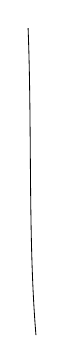
\begin{tikzpicture}[x=1mm,y=1mm]\draw[line width=.3pt] (1,0) .. controls (0,12) and (.5,26) .. (0,39);\end{tikzpicture}}}
\[
\det(\rho+\sigma)=\deleted{\underbrace{\det\rho}_{1}+\underbrace{\det\sigma}_{1}+\operatorname{Tr}(\sigma\rho)}
\]
% R343.05 | deletion | upper middle, lines 5--6 | et la relation équivaut
\deleted{et la relation équivaut}
% R343.06 | display | middle, lines 6--9 | det sigma(1+sigma^{-1}rho)
\[
\begin{aligned}
\unsure{''}\quad
\det\unsure{(}\unsure{\deleted{\rho}\inserted{\sigma}}(1+\sigma^{-1}\rho)
&=\det\sigma\ \underbrace{\det(1+\sigma^{-1}\rho)}_{\underbrace{\det\sigma^{-1}\rho}_{(\det\sigma)^{-1}\det\rho}+\operatorname{Tr}(\underbrace{\sigma^{-1}\rho}_{-\sigma\rho})+1}\\
&=\overbrace{\det\sigma}^{1}+\overbrace{\det\rho}^{1}+\underbrace{\det\sigma}_{1}\operatorname{Tr}(\sigma^{-1}\rho)
\end{aligned}
\]
% R343.07 | margin note | diagonal left margin, beside lines 7--11 | calcul déjà fait
\margin{calcul déjà fait V. p. \unsure{--} ? (cf formule (69))}
% R343.08 | display | middle, line 10 | det(sigma+rho)=2+Tr(sigma^{-1}rho)
\[
\text{i.e.}\qquad\det(\sigma+\rho)=2+\operatorname{Tr}(\sigma^{-1}\rho)=2\unsure{-}\operatorname{Tr}\sigma\rho,\quad\text{donc}
\]
% R343.09 | text | middle, line 11 | la condition det N=0
la condition $\det N=0$ équivaut à (69)
% R343.10 | display | middle, line 12 | Tr sigma rho=2
\[
\operatorname{Tr}\sigma\rho=2
\]
% R343.11 | text | lower, lines 13--17 | Pour prouver cette relation
Pour \deleted{\unsure{la}} prouver cette relation \inserted{(ou des \unsure{versions|voisines} \unsure{testées|telles})}, on peut songer à \deleted{partir}\inserted{procéder} comme tantôt, \unsure{excepté que je} \unsure{suis} parti de (68) au lieu de (75). Ce n'est pas entièrement élucidé -- à revenir à la charge!
% R343.12 | text | bottom left | 342
\mspage{342}
\scanpage{344}
% R344.01 | text | top centre | 473
\mspage{473}
% R344.02 | text | heading | VII Récapitulation sur les épinglages
$\overline{\text{\uline{VII}}}$\quad \uline{Récapitulation sur les épinglages.}
% R344.03 | text | upper, lines 2--4 | On désigne par G,SG,PG
\deleted{\unsure{1)}} On désigne par $G,SG,PG$ des formes de $\mathrm G\ell(2)_S$, $\mathrm S\ell(2)_S$, $\unsure{\mathrm{GP}(1)}_S$ \unsure{associées} à une $\overline{\mathrm m}$ Algèbre d'Azumaya $\mathcal M$, i.e. à un fibré en droites projectives $\unsure{\mathbb P|\mathcal P}$, sur $S$.
% R344.04 | text | subsection heading | Sections régulières de G
1) \uline{Sections régulières de} $G$.
% R344.05 | text | upper middle, line 6 | Soit rho une section
Soit $\rho$ une section de $\unsure{\mathcal M}$ \inserted{(pas néc. inv.)}, posons
% R344.06 | display | upper middle, line 7 | v=det rho,w=Tr rho
\[
(1)\qquad \unsure{v|\nu}=\det\rho,\quad w=\operatorname{Tr}\rho
\]
% R344.07 | text | upper middle, line 8 | de sorte qu'on aura
de sorte qu'on a\deleted{ura} l'équation d'Hamilton-Cayley
% R344.08 | display | upper middle, line 9 | rho^2-w rho+v=0
\[
(2)\qquad \rho^2-w\rho+\unsure{v|\nu}=0\qquad\text{i.e.}\quad\rho^2=w\rho-\unsure{v|\nu}
\]
% R344.09 | text | middle, line 10 | Proposition Conditions équivalentes
\uline{Proposition} Conditions équivalentes:
% R344.10 | text | middle, line 11 | a) rho n'est un scalaire
a) $\rho$ n'est un scalaire sur aucune fibre.
% R344.11 | text | middle, lines 12--13 | a') A_rho=O_S+O_S rho
\unsure{a')} $\mathcal A_\rho=\underline{\mathcal O}_S+\underline{\mathcal O}_S\rho$ est un sous-module \unsure{localmt|localt} facteur direct libre de rang $2$ de $\mathcal M$.
% R344.12 | margin note | left, beside conditions a' and b | NB À cause de (2)
\margin{NB À cause de (2), $\mathcal A_\rho$ est une sous-\uline{Algèbre} de $\mathcal M$.}
% R344.13 | text | middle, lines 14--16 | b) Il existe loc. (Zar)
b) (Si $\mathcal M=\underline{\operatorname{End}}_{\mathcal O_S}(F)$) Il existe loc. (Zar) une section $\unsure{e_0|E_0}$ de $F$ telle que $(e_0,\deleted{\unsure{\rho.}}e_1\mathrel{\overset{\mathrm{dfn}}{=}}\rho(e_0))$ forment une base de $F$
% R344.14 | text | middle-lower, lines 17--18 | b') Il existe loc. Zar
b') (Si $\mathcal M=\underline{\operatorname{End}}_{\mathcal O_S}(F)$) Il existe loc. Zar un ``sous-fibré en droites'' $D_0\subset F$, tel que
% R344.15 | display | middle-lower, line 19 | F=D_0+D_1
\[
F=D_0+D_1,\quad\text{où }D_1=\rho(D_0)
\]
% R344.16 | text | lower, lines 20--22 | b'') Le O_S[T]-module
\unsure{b'')} (Si $\mathcal M=\underline{\operatorname{End}}_{\mathcal O_S}(F)$.) Le $\mathcal O_S[T]$-module $F_\rho$ ($\unsure{:}$ $T$ \unsure{est|étant} une indéterminée, qui opère sur $F$ par $\rho$) est \deleted{\unsure{isomorphe} à $\underline{\mathcal O}_S$} \inserted{\deleted{\unsure{loc$^{\mathrm t}$}} monogène} loc$^{\mathrm t}$ (Zar).
% R344.17 | text | lower, lines 23--24 | c) Le O_S[T]-module
c) (Si $\mathcal M=\underline{\operatorname{End}}_{\mathcal O_S}(F)$) Le $\underline{\mathcal O}_S[T]$-module $F_\rho$ \unsure{est|$\to$} isomorphe à
% R344.18 | display | lower, line 24 | O_S[T]/(T^2-wT+v)
\[
\underline{\mathcal O}_S[T]/(T^2-wT+\unsure{v|\nu})
\]
% R344.19 | text | bottom, lines 25--26 | c') il existe localt Zar une base
c') \inserted{(cas $\mathcal M=\underline{\operatorname{End}}(F)$)} $\exists$ \unsure{loc$^{\mathrm t}$|local$^{\mathrm t}$} Zar une base $e_0,e_1$ de $F$, telle que la matrice de $\rho$ \unsure{p.r.|p.v.} à cette base
% R344.20 | text | bottom left | 343
\mspage{343}
\scanpage{345}

soit
\[
(3)\qquad \rho_{e_0,e_1}=\begin{pmatrix}0&-\unsure{v|\nu}\\1&w\end{pmatrix}
\]
\margin{(i.e. $\rho e_0=e_1$ d'où \deleted{$\rho e_1=$}
$\rho e_1=\unsure{-v\rho e_0-w e_0}$}

c'') \inserted{(Cas $\mathcal M=\underline{\operatorname{End}}_{\underline{\mathcal O}_S}(F)$)}
$\exists$ loc. Zar une base $(e_0,e_1)$ de $F$ telle que la matrice de $\rho$ p.r. à celle-ci soit
\[
(4)\qquad \rho_{e_0,e_1}=\begin{pmatrix}0&1\\-v&w\end{pmatrix}
\]

d) Le commutant de $\rho$ dans $\mathcal M$ est réduit à
$\mathcal A_\rho=\underline{\mathcal O}_S+\underline{\mathcal O}_S\rho$, et il en reste ainsi après chaque chgt de base $S'\to S$.

d') \unsure{Itm|Item} en chaque fibre.

\uline{Dém}\quad $a\Longleftrightarrow a'$ trivial (algèbre linéaire des Modules $\mathcal M$ et des sous-modules $\underline{\mathcal O}_S1$ loc facteur direct)

$b\Longleftrightarrow b'\Longleftrightarrow b''$ trivial, $b)\Longrightarrow a)$ aussi.

$a\Longrightarrow b$ il suffit de choisir $e_0$ \deleted{dans}\inserted{sur} une \deleted{\unsure{corps}}\inserted{fibre} de façon à ne pas être vecteur propre sous $\rho$ (possible sur un corps, pour un op. non scalaire) puis de relever au voisinage.

\inserted{$b\Longleftrightarrow$}$c)\Longleftrightarrow c')$ trivial ; \deleted{$c')\Longleftrightarrow c'')$ \unsure{car les}}\inserted{les bases pour lesquelles}
$\rho_{e_0,e_1}$ soit de la forme $\begin{pmatrix}0&-v\\1&w\end{pmatrix}$ \unsure{st.} justement les bases de la forme $(e_0,e_1=\rho e_0)$.

$c')\Longleftrightarrow c'')$ signifie que si $\rho$ satisfait aux conditions envisagées, ${}^t\rho$ aussi. (\deleted{\unsure{donc}} et inversement il en résulte que la condition pour ${}^t\rho$ l'implique pour $\rho={}^t({}^t\rho)$\deleted{\unsure{$\}$}}, i.e. $c'')\longrightarrow c')$) --- mais c'est immédiat sous la forme a).

Ainsi les conditions a) à c'') sont équivalentes, d'ailleurs $d)\Longrightarrow d')\Longrightarrow a)$ est trivial, reste à prouver que $b$ (p.ex.) $\Rightarrow d)$.
\deleted{Si $u$ commute}\inserted{Comme $b$ \unsure{stable}} par chgt de base, il suffit de voir que

\mspage{344}
\scanpage{346}
\mspage{474}

\deleted{\uline{Corollaire 2}}

\uline{NB}\quad \unsure{En} fait, $G=\underline{\mathcal M}^{*}$ opère sur $\underline{\mathcal M}$ (par autom. intérieurs) ou sur $G$, ou $SG$, via $PG=\underline{\mathcal M}^{*}/\mathbb G_m$, et $PG$ est quotient fppf de $SG$ (et $\unsure{\overline{\mathrm m}|=}$ pour la top. (ét), si 2 inv.).

Donc on voit que \inserted{ds} le critère de conjugaison précédent, dans la formule
\[
(6)\qquad \rho'=\operatorname{int}(\alpha)\rho=\alpha\rho\alpha^{-1},
\]
\unsure{OPs} $\alpha\in\Gamma\unsure{\mathrm S\ell(2)|SG}$.

\deleted{\uline{Proposition} Soit $\unsure{\varepsilon}$}\inserted{\uline{Corollaire 2} Soient} $\rho,\unsure{\zeta|\xi}$ deux sections de $G$, $\rho$ étant régulier. Pour que l'on puisse trouver loc. Zar un $\alpha\in\Gamma G$ tel que
\[
(7)\qquad [\alpha,\rho]=\zeta\qquad\text{i.e.}\quad \alpha\rho\alpha^{-1}=\zeta\rho
\]
il f. et s. qu'on ait

a) $\zeta\rho$ est régulier, i.e. $\zeta$ \deleted{$\unsure{\neq}$} non-homothétique à $\rho^{-1}$ sur aucune fibre

b) $\det\zeta=1$, $\operatorname{Tr}\zeta\rho=\operatorname{Tr}\rho$

(On peut alors prendre $\alpha$ ds $SG$\ldots)

\unsure{Ce n'est|Ce ne sont} que les conditions du cor. 1 \deleted{\unsure{de}} de conjugaison de $\zeta\rho$ à $\rho$, la condition $\det\zeta\rho=\det\rho$ s'écrivant aussi $\det\zeta\det\rho=\det\rho$ i.e. $\det\zeta=1$.

\uline{Corollaire 3} L'indétermination de $\alpha$ dans la résolution de (7) est de la forme $\alpha\mapsto\alpha\uline{t}$, avec $\uline{t}$ section de $\underline{\mathcal A}_\rho^*$, i.e. $t=c\rho+d$, avec $c,d\in\Gamma\underline{\mathcal O}_S$, $\det(c\rho+d)$ inv.
\inserted{i.e. $\boxed{\text{\textcircled{8}}\quad c^2\unsure{v|\nu}+wcd\deleted{\text{inv.}}+d^2\quad\text{inv.}}$}
(où, $v=\det\rho$, $w=\operatorname{Tr}\rho$, cf (1)).

\mspage{345}
\scanpage{347}

si $u$ est une section de $\mathcal M$ \deleted{telle que} qui commute à $\rho$, alors $u=a+b\rho$ $(a,b\in\Gamma\underline{\mathcal O}_S)$. Par a) $a$ et $b$ sont uniques, et cela montre que la question est locale fppf. \unsure{OPs} donc $\mathcal M=\underline{\operatorname{End}}(F)$, $F$ muni d'une base $(e_0,e_1=\rho(e_0))$. \deleted{\unsure{et}} On aura, si
\[
\deleted{ue_1=u\rho e_0=\rho=}
\]
\[
u(e_0)=ae_0+be_1\inserted{{}=u'(e_0)}\qquad
\deleted{\text{posons }u'=a+b\rho}\inserted{\text{où}}\quad u'=a+b\rho,
\]
\[
\deleted{u(e_1)=u\rho(e_0)=\rho\underline{ue_0}=\rho(ae_0+be_1)=a\rho(e_0)+b\rho(e_1)}
\]
et si $u$ \unsure{commute} \deleted{$=ae_1+$} à $\rho$, on aura
\[
u(e_1)=u\rho(e_0)=\rho u(e_0)\deleted{{}=\rho(ae_0+}
\]
de $\overline{\mathrm m}$
\[
u'(e_1)=u'\rho(e_0)=\rho u'(e_0)\qquad\text{car }u'\text{ commute à }\rho
\]
donc
\[
u(e_0)\unsure{=|\neq}\unsure{u(e'_0)|u'(e_0)},\quad u(e_1)=u'(e_1)\qquad\text{donc }u=u',
\]
cqfd.

\uline{Définition :} Une section \inserted{de $\mathcal M$} qui satisfait aux conditions équivalentes de la prop. est dite \uline{régulière}. \unsure{Itm|Item} pour sections de $G$, $SG$, interprétées comme sections de $\mathcal M$ --- \deleted{elles sont} une telle section est régulière ssi en aucun pt, elle n'est un scalaire, i.e. n'est dans le centre. Ceci \unsure{reste|est} stable par multiplication par un scalaire inversible --- d'où par passage au quotient on déduit la notion de section régulière de $PG$ --- ce sont les sections qui ne sont $=1$ en aucune fibre.

\uline{Corollaire 1} Soient $\rho,\rho'$ deux sections \deleted{régulières} de $\mathcal M$, \inserted{$\rho$ étant régulier.} Pour qu'elles soient conjuguées (loc Zar) via $\mathcal M^*$, il f. et s. que \deleted{$\rho$} a) $\rho'$ soit régulier (Condition \inserted{de régularité} \deleted{\illegible{1}}) et b) on ait
\[
(5)\qquad \det\rho=\det\rho',\quad \operatorname{Tr}\rho=\operatorname{Tr}\rho'
\]
(``Condition numérique''

\mspage{346}
\scanpage{348}
\mspage{475}

Ceci résulte de l'équivalence $a)\Longleftrightarrow d)$ de la prop.

\uline{Proposition} Soit
\[
(9)\qquad \varepsilon=1+N
\]
une section de $\mathcal M$. Conditions équivalentes

\[
\text{a)}\quad (10)\quad
\begin{gathered}
\det\varepsilon=\det1\quad(=1)\\
\operatorname{Tr}\varepsilon=\operatorname{Tr}1\quad(=2)
\end{gathered}
\qquad \deleted{\varepsilon\text{ régulier}}\quad\text{et }\varepsilon\text{ régulier}
\]
\margin{\uline{NB}\quad $\det(1+N)=1+\operatorname{Tr}N+\det N$\quad $\operatorname{Tr}(1+N)=2+\operatorname{Tr}N$.}
\[
\text{b)}\quad (11)\quad \det N=\operatorname{Tr}N=0\qquad\text{et }N\text{ régulier}
\]

c) (Si $\mathcal M=\underline{\operatorname{End}}_{\underline{\mathcal O}_S}(F)$) $\exists$ fibré en droites $D\subset F$ tel que l'on ait
\[
N(F)=D,\quad N(D)=0
\]
(Alors $D$ est uniquement déterminé par $\varepsilon$ i.e. par $N$, \deleted{et réciproquement} \inserted{$D$ détermine $N$ mod homothétie})

\inserted{c') (Si $\mathcal M=\underline{\operatorname{End}}_{\underline{\mathcal O}_S}(F)$). $\exists$ loc. \unsure{base|Zar} $e_0,e_1$ tel que $\varepsilon=\begin{pmatrix}1&1\\0&1\end{pmatrix}$ i.e. $N=\begin{pmatrix}0&1\\0&0\end{pmatrix}$}

d) $\exists$ Borel $B\subset G$, tel que $\varepsilon$ soit une section partout $\ne1$ de $B_u$.

d') \deleted{\unsure{Si}}$\exists$ Borel $SB\subset SG$, tel que $\varepsilon$ soit une section partout $\ne1$ de $(SB)_u$.

\deleted{\unsure{Dém}} De plus, $D,B,SB$ sont bien déterminés par $\varepsilon$ i.e. par $N$, et déterminent $N$ à homothétie près.

\uline{Définition :} on \deleted{dit} \unsure{que} $\varepsilon$ est (strictement) unipotent ssi on a $\det\varepsilon=1$, $\operatorname{Tr}\varepsilon=2$, que $N$ est \uline{strictement nilpotent} \unsure{ssi|si} $\det N=\operatorname{tr}N=0$ (d'où $N^2=0$ par Hamilton-Cayley). On dit que $\varepsilon$ est unipotent régulier resp. nilpotent régulier (en laissant tomber le qualificatif ``strictement'') si de plus il est régulier.

\mspage{347}
\scanpage{349}

\uline{Proposition}. Soit $P$ une section de $\mathcal M$. Conditions équivalentes

\[
\begin{aligned}
\text{a)}\quad &P\text{ est régulier, et }P^2=P\\
\text{b)}\quad &\det P=0,\quad\operatorname{Tr}P=1
\end{aligned}
\]

c) (Si $\mathcal M=\underline{\operatorname{End}}_{\underline{\mathcal O}_S}(F)$) $\exists$ base $e_0,e_1$ de $F$ telle que la matrice de $P$ soit
\[
P_{e_0,e_1}=\begin{pmatrix}0&0\\0&1\end{pmatrix}\qquad\text{i.e.}
\]
$P$ soit la projection de $\underline{\mathcal O}_S e_0\oplus\underline{\mathcal O}_S e_1$ sur le facteur $\underline{\mathcal O}_S e_1$

\diagram{\begin{tikzcd}[column sep=small,row sep=large,ampersand replacement=\&]
\text{d)} \& \text{\parbox{0.83\linewidth}{$\exists$ \inserted{(loc. Zar)} isom $\mathcal M\xleftarrow[\sim]{\unsure{\varphi|\psi}}\mathrm M_2(\underline{\mathcal O}_S)$, transformant $\begin{pmatrix}0&0\\0&1\end{pmatrix}$ en $P$.}} \\
\text{c')}\arrow[u,bend left=55] \& \text{\parbox{0.83\linewidth}{(Si $\mathcal M=\underline{\operatorname{End}}_{\underline{\mathcal O}_S}(F)$) $P$ est un projecteur dont l'image \inserted{$D_1$} et le noyau \inserted{$D_0$} sont de rang $1$.}}
\end{tikzcd}}

\uline{Rmq} \deleted{\unsure{Corol}} Pour la démonstration, on notera que la condition numérique b) implique déjà que $P$ est régulier, car si $P$ était un scalaire $\lambda$ (sur une fibre) on aurait
\[
\det P=\lambda^2=0,\quad\operatorname{Tr}P=2\lambda=1
\]
donc $\lambda$ serait inversible et serait de carré nul, absurde. Noter que cet argument montre, plus généralement, que si $\rho$ est une section de $\mathcal M$ telle que
\[
(12)\qquad \delta(\rho)=(\operatorname{Tr}\rho)^2-4\det\rho=w^2-4\unsure{v|\nu}
\]
\margin{($=$ discriminant du polynôme de Hamilton-Cayley de $\rho$)}
soit une section inversible de $\underline{\mathcal O}_S$, alors $\rho$ est une section \uline{régulière} de $\mathcal M$.

\deleted{\uline{Corollaire}} Les $P$ \deleted{\unsure{en}} satisfaisant les condit. de la proposition précédente sont appelés les \uline{projecteurs élémentaires} dans $\mathcal M$. \unsure{Dém.|leur.}

\uline{Corollaire} On a une corr. biunivoque entre les projecteurs élémentaires dans $\mathcal M$, et les couples de Killing $(B,T)$ dans $G$ (ou $SB,ST$ dans $SG$, ou $PB,PT$ dans $PG$), en

\mspage{348}
\scanpage{350}
\mspage{476}

associant à \deleted{$\unsure{N}$} $P$ le \deleted{\unsure{sous}} tore
$T=\underline{A}_P^*$, et le
\inserted{Borel $B_0$}
\deleted{sous-groupe unipotent}
\deleted{\inserted{additif}}
formé des $\unsure{\alpha}$ qui stabilisent
\deleted{\unsure{le} drapeau} $D_0$
\deleted{et \unsure{induisent}}
\deleted{\inserted{\unsure{le couple des}}}
\deleted{l'identité sur $D_0$ et sur $F/D_0\simeq D_1$,}
\inserted{donc \unsure{p.r.|p.v.}}
\deleted{donc formé des}
\deleted{\unsure{commutant} à $N$.}
à $e_0,e_1$ on aura
\[
(13)\qquad
\left\{
\begin{aligned}
T&=\left\{\begin{pmatrix}\mu_0&0\\0&\mu_1\end{pmatrix}
\ \middle|\ \mu_0,\mu_1\in\Gamma G_m\right\},\\
B_0&=\left\{\begin{pmatrix}\mu_0&\lambda\\0&\mu_1\end{pmatrix}
\ \middle|\ \mu_0,\mu_1\in\Gamma G_m,\ \lambda\in\Gamma G_a\right\}.
\end{aligned}
\right.
\]

Le couple de Killing \uline{opposé} à $(T,B_0)$ est
$(T,B_1)$, avec
\[
(14)\qquad
B_1=\left\{\begin{pmatrix}\mu_0&0\\\lambda&\mu_1\end{pmatrix}
\ \middle|\ \mu_0,\mu_1\in\Gamma G_m,\ \lambda\in\Gamma G_a\right\},
\]
de façon un peu plus intrinsèque, $B_1$
\deleted{\unsure{aura}} est le stabilisateur de $D_1$.
Le proj. él. associé au couple de Killing
\inserted{\uline{opposé} $(T,B_1)$} est $1-N$.

\uline{Remarque}. Le schéma des $\varepsilon_{\unsure{1}}$
\inserted{unipotents réguliers, ou encore des $N$ \unsure{nilp.} \unsure{régul.}}
est un fibré en droites épointées (i.e. un $G_m$-torseur)
sur le schéma \inserted{$\mathcal P$} des Borels
(de $G$, de $SG$ ou de $PG$, cela revient au $\unsure{\overline{\mathrm m}|=}$),
il est \deleted{de dim} lisse de dim relative $2$ — le schéma des
projecteurs élémentaires $N$ est \deleted{lisse} isom.
à celui des couples de Killing, fibré-lisse de dim relative $1$
sur le schéma des Borels. Le \deleted{fibré} produit fibré de
ces deux schémas \inserted{relatifs} au dessus de
$\mathcal P=$ schéma des Borels, est isomorphe au schéma
des épinglages de $G$ (ou de $SG$, ou de $PG$)
i.e. des iso $\mathrm{G}\ell(2)_S\xrightarrow{\sim}G$
(resp. $\mathrm{S}\ell(2)_S\xrightarrow{\sim}SG$,

\mspage{349}
\scanpage{351}

resp. $\unsure{\mathrm{GP}(1)}_S\xrightarrow{\sim}PG$),
qui est un torseur sur
$\mathrm{GP}(1)_S\simeq
\underline{\mathrm{Aut}}_{S-\unsure{\mathrm{gr}}}\mathrm{G}\ell(2)_S
\simeq\underline{\mathrm{Aut}}_{S-\unsure{\mathrm{gr}}}\mathrm{S}\ell(2)_S
\simeq\underline{\mathrm{Aut}}_{S-\unsure{\mathrm{gr}}}
(\mathrm{GP}(1)_S)$.
On dit que $\varepsilon$ et \deleted{$\unsure{N}$}$P$ sont
\uline{associés},
\inserted{(ou $N=\varepsilon-1$ et $P$ sont associés),}
s'ils définissent le $\unsure{\overline{\mathrm m}|=}$ Borel,
i.e. \deleted{définissent}
\deleted{\unsure{prov.}}\inserted{proviennent} d'un épinglage.
On vérifie que ceci revient aux relations suivantes
\[
(15)\qquad PN=0,\qquad NP=N
\]
\deleted{(16)} ou encore, en termes de $P$ et $\varepsilon=1+N$
\[
(16)\qquad P\varepsilon=P,\qquad
\varepsilon P=P+\underbrace{\varepsilon-1}_{N}
\]
\margin{C'est \unsure{vraiment} \unsure{joli} !}

Nous considérons maintenant la question de
\deleted{\unsure{l'équi.}}\inserted{la} conjugaison des sections
$\widetilde\rho,\widetilde\rho'$ de $PG$,
définies par des sections $\rho,\rho'$ de $G$.
On suppose $\widetilde\rho$ régulière i.e. $\ne1$ en
chaque \deleted{pt} fibre, i.e. $\rho$ régulière —
\deleted{\unsure{Une}}
\deleted{\unsure{une}} la conjugaison
\inserted{de $\widetilde\rho,\widetilde\rho'$}
par une section $u$ de $G$ (disons) signifie qu'on a
\[
(17)\qquad \rho'=\lambda u\rho u^{-1},\qquad
\lambda\in\Gamma G_m
\]
d'où on déduit
\[
\det\rho'=\lambda^2\det\rho\qquad
\operatorname{Tr}\rho'=\lambda\operatorname{Tr}\rho
\]
et par suite
\[
(18)\qquad
\frac{\operatorname{Tr}^2\rho'}{\det\rho'}
=\frac{\operatorname{Tr}^2\rho}{\det\rho}.
\]
Posons, pour une section de $G$
\[
(19)\qquad
\deleted{\unsure{\delta|\Delta}(\rho)=}
\Delta(\rho)=\frac{\operatorname{Tr}^2\rho}{\det\rho},
\]

\mspage{350}
\scanpage{352}
\mspage{477}

on a fait ce qu'il fallait pour \unsure{qu'on}
\unsure{trouve} un $G\longrightarrow \mathbb E^1$ qui passe au
quotient en
\[
(20)\qquad
\begin{gathered}
PG\xrightarrow{\Delta}\mathbb E^1\\
\Delta(\widetilde\rho)=\Delta(\rho)
=\frac{(\operatorname{Tr}\rho)^2}{\det\rho},
\end{gathered}
\]
et qui \unsure{soit|reste} invariant par autos int.

\uline{Proposition}. Pour que deux sections
$\widetilde\rho,\widetilde\rho'$ de $PG$ soient
\deleted{\unsure{équi}} conjuguées loc. fppf,
\inserted{$\widetilde\rho$ étant régulière,}
il f. \deleted{\unsure{et s.}}
que $\widetilde\rho'$ soit \uline{régulière}, et qu'on ait
\margin{$\Big|$}
\[
(21)\qquad
\Delta(\widetilde\rho')=\Delta(\widetilde\rho)
\]
i.e. (en termes de $\rho,\rho'$ relevant
$\widetilde\rho,\widetilde\rho'$) que $\rho'$ soit
régulière et satisfasse (18).
Ces conditions sont suffisantes quand
$\Delta(\widetilde\rho)$ inv. i.e. $\operatorname{Tr}\rho$ inv.
Il reste à prouver la suffisance. Notons que loc. fppf,
existe $\lambda$ \inserted{$\in\Gamma G_m$} telle que
\[
\det(\rho')=\det(\lambda\rho)\qquad
\text{i.e.}\quad\lambda^2=\frac{\det\rho'}{\det\rho}.
\]
Donc \unsure{OPS} (quitte à remplacer $\rho$ par $\lambda\rho$)
que $\det\rho=\det\rho'$.
Alors (18) revient à
\[
(22)\qquad
\operatorname{Tr}^2\rho'=\operatorname{Tr}^2\rho.
\]
\deleted{Cela} la question revient à voir que
$\exists\varepsilon\in\Gamma\mu_2$, telle que
\[
\operatorname{Tr}\rho'=\varepsilon\operatorname{Tr}\rho
\quad(=\operatorname{Tr}\varepsilon\rho),
\]
on aura aussi
\[
\det\rho'=\det\varepsilon\rho
\quad(=\underbrace{\varepsilon^2}_{1}\det\rho=\det\rho),
\]
d'où loc. conjugaison de $\rho'$ et $\varepsilon\rho$,
on aura terminé. Mais si $\tau',\tau$ sont deux sections de
$\mathcal O_S$, avec $\tau$ \uline{inv.}, telles que
$\tau'^2=\tau^2$, on aura bien
$\tau'=\varepsilon\tau$ $(\varepsilon=\tau'/\tau)$,
et $\varepsilon^2=1$, OK.

\mspage{351}
\scanpage{353}

\uline{Rmq}. Si $\Delta(\rho)$ non inv. il y a des
contre-exemples évidents, p.ex. avec
$(\operatorname{Tr}\rho)^2=0$,
$(\operatorname{Tr}\rho')^2=0$,
$\det\rho=\det\rho'=1$,
$\operatorname{Tr}\rho$ et $\operatorname{Tr}\rho'$
n'étant pas homothétiques. On peut prendre
\[
\rho=\begin{pmatrix}0&1\\-1&w\end{pmatrix},
\qquad
\rho'=\begin{pmatrix}0&1\\-1&w'\end{pmatrix}
\]
$w^2=w'^2=0$, $w,w'$ non homothétiques, p.ex.
anneau de base
$A=A_0[w,w']/(w^2,ww',w'^2)$
(\unsure{nbs|nbres} duaux sur le module libre de rg $2$
engendré par $w,w'$).

$2)$ Position relative de deux sections $\rho,\sigma$
de $G$, ou $\widetilde\rho,\widetilde\sigma$ les deux sections de $PG$.
\margin{$\big|$}

On s'intéresse dans $PG$ à
\[
(23)\qquad
\widetilde\varepsilon_0
=\widetilde\sigma^{-1}\widetilde\rho
\quad\text{et}\quad
\widetilde\varepsilon_1
=\widetilde\rho\widetilde\sigma^{-1}
=\widetilde\rho(\widetilde\varepsilon_0)
=\widetilde\sigma(\widetilde\varepsilon_1)
\]
et à la condition que
\inserted{\textcircled{\(1^\circ\)}}
$\widetilde\varepsilon_0$,
\deleted{\unsure{$\widetilde\varepsilon_1$, tous deux}}
\inserted{(donc $\widetilde\varepsilon_1$)}
\unsure{soit|sont} unipotent régulier —
donc \inserted{$\widetilde\varepsilon_0,\widetilde\varepsilon_1$}
proviennent canoniquement des
$\varepsilon_0,\varepsilon_1$ unipotents réguliers de $SG$,
satisfaisant
\[
(24)\qquad
\varepsilon_1=\widetilde\rho(\varepsilon_0)
=\widetilde\sigma(\varepsilon_0)
\]
\[
(25)\qquad
\left\{
\begin{aligned}
\varepsilon_0&=(\text{Scalaire inv.})\,\sigma^{-1}\rho\\
\varepsilon_1&=(-\ -\ -\ -)\,\rho\sigma^{-1}
\end{aligned}
\right.
\]
\margin{pour un \unsure{relèvement} \unsure{plus}
\unsure{commode|conv.} de $\sigma$ et $\rho$}
\margin{soit
$\varepsilon_0=-\deleted{\unsure{\lambda_0}}\sigma^{-1}\rho$,
$\varepsilon_1=-\deleted{\unsure{\lambda_0}}\rho\sigma^{-1}$}
et \textcircled{\(2^\circ\)}
$\widetilde\varepsilon_0,\widetilde\varepsilon_1$ soient
\deleted{partout}\inserted{en chaque fibre}
"non équivalents",
i.e. \deleted{$\varepsilon_0=$}, posons
\[
(26)\qquad
\varepsilon_0=1+N_0,\qquad
\varepsilon_1=1+N_1
\]

\mspage{352}
\scanpage{354}
\mspage{478}

que $N_0$ et $N_1$ soient partout
\unsure{non-homothétiques|non homothétiques}.

Alors $\widetilde\varepsilon_0(\mathbb G_a)$,
$\widetilde\varepsilon_1(\mathbb G_a)$,
$\widetilde\varepsilon_0\in\Gamma
\widetilde\varepsilon_0(\mathbb G_a)$ définissent
un \deleted{\unsure{scindage}}
\inserted{épinglage} canonique de $PG$ donc de $G$ \ldots
\inserted{On aura alors, pour cet épinglage}
\deleted{La situation est}
\[
(26)\qquad
\rho=\begin{pmatrix}0&u\\v&w\end{pmatrix}
\qquad
\sigma=\begin{pmatrix}0&u'\\v'&w'\end{pmatrix}
\]
avec $u,v,u',v'\in\Gamma(\mathbb G_m)$,
$w,w'\in\Gamma\mathbb G_a$,
\deleted{$\unsure{\rho}$}

et on aura
\[
(27)\quad
\left\{
\begin{aligned}
-\sigma^{-1}\rho
&=\begin{pmatrix}
-\dfrac{v}{v'}&
\dfrac{uw'-wu'}{u'v'}\\
0&-\dfrac{u}{u'}
\end{pmatrix}
=\varepsilon_0
=\begin{pmatrix}1&\unsure{?}\\0&1\end{pmatrix}\\[1ex]
-\rho\sigma^{-1}
&=\begin{pmatrix}
-\dfrac{u}{\unsure{w'|u'}}&0\\
\dfrac{vw'\unsure{-|+}wv'}{\unsure{w'|u'}v'}&-\dfrac{v}{v'}
\end{pmatrix}
=\varepsilon_1
\overset{\inserted{\unsure{\mathrm{déf.}}}}{=}
\begin{pmatrix}1&0\\\unsure{1}&1\end{pmatrix}
\end{aligned}
\right.
\]
\margin{par définition de notre épinglage}

donc il faudra
\[
(28)\qquad
u/u'=-1,\quad v/v'=-1,\qquad
\text{i.e.}\quad u'=-u,\ v'=-v
\]
\deleted{$(29)\quad\dfrac{vw'\unsure{+|-}wv}{uv}$}
donc
\[
-\rho\sigma^{-1}
=\begin{pmatrix}1&0\\\dfrac{1}{u}(w'+w)&1\end{pmatrix}
\]
et il faut
\[
(29)\qquad w'+w=u
\qquad\text{i.e.}\qquad w'=w-u
\]
en d'autres termes \unsure{croisant} $(26)(27)$
\[
(30)\qquad \rho+\sigma=uP
\quad\text{où}\quad
P=\begin{pmatrix}0&0\\0&1\end{pmatrix}
\]
est le projecteur élém. associé à l'épinglage envisagé.
\margin{ce qui détermine $\sigma$ en termes de $\rho$,
\deleted{et} du \unsure{coeff.} $u$ de $\rho$, et de $P$}

Et on aura
\[
(31)\qquad
-\sigma^{-1}\rho=\varepsilon_0
=\begin{pmatrix}1&u/v\\0&1\end{pmatrix},
\qquad
N_0=\begin{pmatrix}0&u/v\\0&\unsure{0|1}\end{pmatrix}
\]

\mspage{353}
\scanpage{355}

On aimerait donner des ``critères numériques'' intrinsèques pour que $\rho,\sigma$ aient les propriétés précédentes\ldots

\uline{Proposition} Soient $\rho,\sigma$ deux sections \inserted{\deleted{\unsure{régulières}}} de $G$,

\deleted{Conditions équivalentes} \inserted{\unsure{Posons}}
\[
\unsure{\varepsilon}\qquad \varepsilon_0=-\sigma^{-1}\rho,\qquad \varepsilon_1=-\rho\sigma^{-1}
\]
de sorte qu'on ait donc
\[
\varepsilon_1=\sigma(\varepsilon_0)=\rho(\varepsilon_0).
\]

Conditions équivalentes

$a)$ \inserted{$1^\circ)$} $\varepsilon_0$ \deleted{et $\varepsilon_1$} \deleted{\unsure{sont}} \inserted{est} \unsure{unipotents|unipotent} \unsure{réguliers|régulier} \deleted{\unsure{partout}} \inserted{$(\Leftrightarrow\varepsilon_1$} unipotent régulier) et \inserted{$2^\circ)$} $\varepsilon_0$ et $\varepsilon_1$ \deleted{partout} \deleted{\unsure{non équivalents, i.e.}} indépendants \inserted{en chaque fibre}, --- i.e. posant
\[
\varepsilon_0=1+N_0,\qquad \varepsilon_1=1+N_1
\]
$N_0$ $(\Leftrightarrow N_1)$ est nilpotent régulier, et $N_0$ et $N_1$ sont partout non homothétiques.

$b)$ On a
\[
\begin{array}{rl}
\deleted{\unsure{(32)}}&\\[-1.2em]
(32)&\left\{\begin{array}{l}
\left.\begin{array}{ll}
a)&\det\sigma=\det\rho\\
b)&\operatorname{Tr}\sigma^{-1}\rho=-2
\end{array}\right\}\\
c)\quad u\overset{\mathrm{dfn}}{=}\operatorname{Tr}(\sigma+\rho)\text{ est inversible}
\end{array}\right.
\end{array}
\]
\deleted{$\unsure{(33)}$} \deleted{$\unsure{(34)}$}
\margin{ces deux relations expriment $\det(\varepsilon_0)=1$, $\operatorname{Tr}\varepsilon_0=2$ i.e. $\varepsilon_0$ est \deleted{(strictement)} unipotent}
\margin{ceci exprime que $\varepsilon_0$ est régulier et indépendant de $\varepsilon_1$, cf loc. cit.}
\margin{cf prop. p. $449'$}

$c)$ On a \deleted{$\det\sigma=\det\rho$}
\[
(33)\quad\left\{\begin{array}{ll}
a)&\det\sigma=\det\rho\\
b)&\det(\sigma+\rho)=0\\
c)&\operatorname{Tr}(\sigma+\rho)\text{ inversible}
\end{array}\right.
\]

$d)$ On a $\det\sigma=\det\rho$, et il existe un projecteur élémentaire $P$ et un scalaire inv. $u\in\Gamma\mathbb G_{\mathrm m}$, tels que l'on ait
\[
(34)\qquad \sigma+\rho=uP
\]
\margin{\uline{NB} $P$ et $u$ sont uniquement déterminés, $u=\operatorname{Tr}(\sigma+\rho)$, $P=\frac1u(\sigma+\rho)$}

\mspage{354}
\scanpage{356}
\mspage{479}

\deleted{$e)$ (Si $M=\underline{\operatorname{End}}(F)$) $\exists$ une base de $F$, telle que par rapport à cette base on ait}

$e)$ $\exists$ isomorphisme $\mathrm{G}\ell(2)\overset{\varphi}{\xrightarrow{\sim}}G$, \inserted{\deleted{(unique)}} tel que l'on ait
\[
(35)\quad\left\{\begin{aligned}
\varphi^{-1}(\varepsilon_1)&=\begin{pmatrix}1&0\\1&1\end{pmatrix}\\
\varphi^{-1}(\varepsilon_0)&=\begin{pmatrix}1&\deleted{\unsure{1}}\unsure{?}\\0&1\end{pmatrix}
\end{aligned}\right.
\]
\margin{\uline{NB} cet isom est unique}

$f)$ $\exists$ isom. $\mathrm{G}\ell(2)\simeq G$ tel que l'on ait
\[
(36)\quad\left\{\begin{gathered}
\varphi^{-1}(\rho)=\begin{pmatrix}0&u\\v&w\end{pmatrix}\qquad
\varphi^{-1}(\sigma)=\begin{pmatrix}0&\unsure{w'|u'}\\v'&w'\end{pmatrix}\\
\text{avec}\qquad u+u'=v+v'=0,\qquad w+w'=u
\end{gathered}\right.
\]
\margin{\uline{NB} On aura $P=\begin{pmatrix}0&0\\0&1\end{pmatrix}$}
\margin{cet $\varphi$ est encore unique; On aura
\[
(37)\quad\left\{\begin{aligned}
u&=\operatorname{Tr}(\sigma+\rho)\;(=-u')\\
w&=\operatorname{Tr}\rho\quad(w'=\operatorname{Tr}\sigma)\\
-uv&=\det\rho=\det\sigma
\end{aligned}\right.
\]
ce qui décrit $u,\unsure{w},\unsure{v}$ en termes de $\rho$, donc aussi $u',v',w'\ldots$}

\deleted{$\unsure{(37)}$}

On aura dans (35), avec
\[
\unsure{(38)}\qquad\varphi^{-1}(\varepsilon_0)=\begin{pmatrix}1&u/v\\0&1\end{pmatrix},
\]
et on aura
\[
(39)\qquad\sigma+\rho=uP,\quad\text{avec }\varphi^{-1}(P)=\begin{pmatrix}0&0\\0&1\end{pmatrix}.
\]

Démonstration facile. L'équivalence $a)\Leftrightarrow b)$ \unsure{vu|vue} dans prop. p. $449'$. Pour $b)\Leftrightarrow c)$, on écrit
\[
\begin{aligned}
\unsure{\det}(\sigma+\rho)
&=\det\{\sigma(1+\sigma^{-1}\rho)\}
=\det\sigma\;\underbrace{\det(1+\sigma^{-1}\rho)}_{1+\operatorname{Tr}\sigma^{-1}\rho+\underbrace{\det\sigma^{-1}\rho}_{(\det\sigma)^{-1}\det\rho}}\\
&=\\
&=\det\sigma+\det\rho+(\det\sigma)\operatorname{Tr}(\sigma^{-1}\rho)
\end{aligned}
\]
donc en vertu de l'hyp
\[
\det\sigma=\det\rho
\]
commune à $b)$ et $c)$, \unsure{on aura}
\[
(\unsure{*|6})\qquad\det(\sigma+\rho)=\det\sigma\,(2+\operatorname{Tr}(\sigma^{-1}\rho))
\]
donc le premier \unsure{mb|membre} est nul ssi $\operatorname{Tr}\sigma^{-1}\rho=-2$, qfd.

\mspage{355}
\scanpage{357}

Posant $Q=\sigma+\rho$, l'équivalence $b\Leftrightarrow c$ provient de l'équivalence (valable pour tte section $Q$ de $M$)
\[
(40)\quad (\det Q=0,\operatorname{Tr}Q\text{ inv.})\Longleftrightarrow
\left(\begin{gathered}\exists\text{ projecteur élém. }P,\text{ et }u\in\Gamma\mathbb G_{\mathrm m},\\
\text{tels que }Q=uP\end{gathered}\right)
\]
qui résulte facilement des résultats du n\textsuperscript{o} précédent (c'est un corollaire de la prop. p. $475'$, que j'ai oublié d'expliciter.

L'équivalence avec $e)$, $f)$ est aussi immédiate, \deleted{\unsure{c'est en|c'est un}} et ne fait que résumer certains calculs précédents.

\margin{\uline{Corollaire} Sous ces conditions $1,N_0,N_1,P$ forment une \uline{base} de $M$, et $\rho$ et $\sigma$ sont combin. lin. indépendantes de \deleted{$\unsure{N_0}$} $N_0,N_1,P$
\[
\left\{\begin{aligned}
\rho&=v(N_0+N_1)+wP\\
\sigma&=-v(N_0+N_1)+(u-w)P
\end{aligned}\right.
\]
$\rho,\sigma$ forment une base \unsure{évidemment|évidente} du \unsure{sous-Module|sous-module} de $M$ engendré par $(N_0+N_1)$ et $P$, donc
\[
\rho,\sigma,N_0,1\qquad\text{et}\qquad\rho,\sigma,N_1,1
\]
forment aussi des bases de $M$, et on peut y remplacer soit $\rho$, soit $\sigma$ par $P$; i.e. dans $N_0,N_1,P,1$ on peut \unsure{remplacer} $N_0$, ou $N_1$ par $\rho$ ou $\sigma$.}

\figure{\begin{tikzpicture}[x=1cm,y=1cm]
\draw[->] (0,1.5) .. controls (-0.15,0.75) and (0.45,0.6) .. (1.05,0.85) -- (-0.05,-0.9);
\end{tikzpicture}}

Notre point de vue ici est que nous partons de $\widetilde\rho,\widetilde\sigma_{\unsure{1}}$, que nous voulons décrire --- l'épinglage \unsure{est} en effet défini déjà en termes de $\widetilde\rho,\widetilde\sigma$, mais il reste la question de normaliser les relèvements de $\widetilde\rho,\widetilde\sigma$ en $\rho,\sigma$. On a déjà fait une première restriction par les formules
\[
\varepsilon_1=-\sigma^{-1}\rho
\]
en éliminant le \inserted{\uline{facteur}} scalaire $\lambda_0$ --- on peut \unsure{normaliser|simplifier} plus en multipliant $\rho,\sigma$ par le facteur $u^{-1}$, de façon à obtenir l'écriture simple.
\[
(40)\qquad\operatorname{Tr}(\rho+\sigma)=1\quad\text{i.e. }\operatorname{Tr}\rho+\operatorname{Tr}\sigma=1\quad\text{i.e. }u=1,
\]
ce qui signifie donc que $\rho,\sigma$ sont de la

\mspage{356}
\scanpage{358}
\mspage{480}

forme
\[
(41)\qquad \rho=\begin{pmatrix}0&1\\v&w\end{pmatrix},\qquad
\sigma=\begin{pmatrix}0&-1\\v'&w'\end{pmatrix}
\]
\[
v+v'=0,\quad w+w'=1\qquad\text{i.e. }v'=-v,\quad w'=1-w,
\]
donc
\[
(42)\qquad\varepsilon_0=\begin{pmatrix}1&1/v\\0&1\end{pmatrix},
\]
où on a identifié, par $\varphi$, $\mathrm{G}\ell(2)_S$ et $G$.

\deleted{On \unsure{notera} que $\varepsilon_1$ est \unsure{entièrement déterminé}}
\inserted{Y. a-t-il unicité de $\rho,\sigma$ en termes de $\widetilde\rho,\widetilde\sigma$,}
\deleted{\unsure{par}} par les conditions $\varepsilon_1=-\rho\sigma^{-1}$ (i.e. $\varepsilon_0=-\sigma\rho^{-1}$) et (40)?
Je voudrais d'abord vérifier avec soin une assertion faite par la bande un certain nb de fois, savoir que le \deleted{application} \inserted{morphisme}
\[
G\longrightarrow PG\simeq G/\mathbb G_{\mathrm m}
\]
induit une \uline{bijection}

(43)\quad
\diagram{\begin{tikzcd}[column sep=large,ampersand replacement=\&]
\begin{array}{c}\text{unipotents }\deleted{\unsure{stri.}}\\\text{réguliers de}\\G\end{array}
\arrow[r] \&
\begin{array}{c}\text{unipotents}\\\text{\uline{réguliers}}\\\text{de }PG\end{array}
\end{tikzcd}},

(au moins localement \deleted{\unsure{fppf}} \inserted{\unsure{fppf}} \deleted{\unsure{Zar.}})

la surjectivité de cette application pourrait ici servir de \uline{définition} aux unipotents réguliers de $PG$. Donc il s'agit de tester l'\uline{injectivité}, ce qui signifie aussi \deleted{que} ceci: si $\varepsilon,\varepsilon'$ sont deux sections unipot. régulières de $M$, telles que \inserted{$\widetilde\varepsilon=\widetilde\varepsilon'$ i.e.} $\varepsilon'=\lambda\varepsilon$ $(\lambda\in\Gamma\mathbb G_{\mathrm m})$, alors $\varepsilon=\varepsilon'$, \inserted{i.e. $\lambda=1$.} Prenant les déterminants des deux mbs, on aura
\[
(44)\qquad\lambda^2=1,
\]
\margin{Donc, on dira qu'une section de $PG$ est unipotente \unsure{rég} si elle est loc. fppf l'image d'une section unip. régulière de $G$.}

\mspage{357}
% ===== LM_C3-359-377: second pass, checked against the scans =====
\scanpage{359}
prenant les traces on trouve
\[
  2\lambda=2 \tag{45}
\]

--- ce sont les conditions néc. et suff. sur $\lambda$ pour que
\deleted{\unsure{$\lambda$}}
($\varepsilon$ étant unipot. régulier)
$\lambda\varepsilon$ soit encore \inserted{\unsure{str\textsuperscript{t}}}
\unsure{unip.\textsuperscript{t}} (donc néc.\textsuperscript{t} unipotent régulier).
Si $2$ est inv. sur $S$, \inserted{\uline{plus gén.}
si $2$ est section régulière de $\underline{\mathcal O}_S$,}
\deleted{\unsure{est réduit}}
ces conditions impliquent $\lambda=1$, OK, mais
\deleted{\unsure{dans le cas}}\inserted{en dehors} de cette hypothèse (p.ex. en car. $2$
\deleted{\unsure{quitte}} sur un schéma non réduit) il n'en est plus néc. ainsi. Écrivons
\[
  \lambda=1+\nu
\]
les conditions (44) (45) s'écrivent
\[
  2\nu=0,\quad \nu^2=0, \tag{46}
\]
donc pour que sur $S$ l'application (43) soit injection, il f. et s.
que les \inserted{seules} sections de $S$ qui satisfont (46)
sont la section nulle.

En général, désignant par $\mu'_2$ le sous-schéma
en groupes de $\mu_2$ défini par (45)
(c'est en fait un \inserted{schéma en} groupe infinitésimal absolu,
\deleted{\unsure{sur}} \inserted{fini sur $\mathbb Z$, pas plat sur $\mathbb Z$,}
isom. au spectre de
\[
  \mathbb Z[T]/(T^2-1,2T-2)\simeq
  \mathbb Z[S]/(S^2,2\unsure{S}),
\]
isomorphe aussi au schéma des nbs duaux sur $\mathbb Z$,
relatif au module $\mathbb Z/2\mathbb Z$ sur $\mathbb Z$,
\deleted{\unsure{$\mu'_2\simeq$}}
\[
  \mu'_2\simeq\operatorname{Spec}
  \bigl(\mathbb Z\deleted{\unsure{\varepsilon}}\oplus\underbrace{\mathbb Z/2\mathbb Z}_{\text{idéal de carré nul}}\bigr)
  \quad\ldots
\]
\mspage{358}

% Printed archive footer outside the manuscript frame:
% 358
% https://grothendieck.umontpellier.fr
% Université de Montpellier, UMR CNRS 5149, Case courrier 051, Place Eugène Bataillon
% 34095 Montpellier cedex 5 - France
\scanpage{360}
\mspage{481}
Il se trouve que $\mu'_{2S}$ opère
\inserted{librement par translations}
sur le schéma des unipotents réguliers \inserted{\unsure{(ou non)}}
de $G$, et on a
\[
\diagram{\begin{tikzcd}[ampersand replacement=\&]
\underline{\mathrm{Unip.rég}}(G)/\mu'_{2S}
  \arrow[r,"\sim"] \& \underline{\mathrm{Unip.rég}}(PG)
\end{tikzcd}}\ . \tag{47}
\]
Ceci semble à première vue en contradiction avec la \unsure{suite} des Borels
\[
\diagram{\begin{tikzcd}[ampersand replacement=\&,column sep=small,row sep=large]
\deleted{\unsure{1}} \& B \arrow[d,mapsto]
 \& \underline{\mathrm{Borels}}(G)
   \arrow[r,"\sim","B\mapsto B/\mathbb \mathbb G_m"']
   \arrow[d,"\wr"']
 \& \mathrm{Borels}(PG) \arrow[d,"\wr"]
 \& \deleted{\unsure{B}}\widetilde B \arrow[d,mapsto] \\
 \& B_u
 \& \begin{gathered}\text{``Sous-groupes}\\
     \deleted{\unsure{\mathrm U}}\text{unipot. à 1}\\
     \text{param.'' de }G\end{gathered}
     \arrow[r,"\sim"]
 \& \begin{gathered}\text{``Sous-groupes}\\
     \text{unip. à 1 par.''}\\\text{de }PG\end{gathered}
 \& \widetilde B_u \\
 \& \& \text{\unsure{c.à.d.}}\quad L \arrow[r,mapsto,"\sim"] \& p(L)
\end{tikzcd}} \tag{48}
\]
(où $p:G\to PG$ est le morphisme can.\textsuperscript{q})

La difficulté proviendrait-elle du fait que les flèches verticales
(surjectives, par définition de la notion de ``ss-groupes unipot. à 1 paramètre''
de $G$ ou de $PG$) ne seraient pas injectives, en dehors de l'hyp. $2$ inv.
(i.e. car \unsure{rés.}\ $\ne2$)?
J'ai envie de dire que
\[
  \underline B=\operatorname{Norm}(B_u),\quad
  \widetilde B=\operatorname{Norm}(\widetilde B_u) \tag{49}
\]
sont des formules qui permettent de retrouver $B,\widetilde B$ à l'aide
de $B_u,\widetilde B_u$\unsure{,|»} --- et j'ai
\deleted{\unsure{fait}} bien \uline{\unsure{déjà}}
vérifié la première de ces formules, à coups d'alg. lin. dans $M$
(sous la forme : les sous-groupes unipot. à 1 paramètre de $G$
correspondent $1$-$1$ aux sections de $\mathbb P$ sur $S$,
i.e. aux \unsure{ssfibrés} en droites $D$ de $F$\ldots) ---
\mspage{359}

% Printed archive footer outside the manuscript frame:
% 359
% https://grothendieck.umontpellier.fr
% Université de Montpellier, UMR CNRS 5149, Case courrier 051, Place Eugène Bataillon
% 34095 Montpellier cedex 5 - France
\scanpage{361}
mais \unsure{ce même} point dans $PG$, c'est
\deleted{si $u\in\Gamma M^*$ est tel que
$u\widetilde N u^{-1}=\mu N+\lambda$,}
\inserted{pas très trivial.}
\deleted{avec $\mu\in\Gamma\mathbb \mathbb G_m$,}

La difficulté doit plutôt provenir du fait \unsure{qu'une|qu'aucune}
section \unsure{unipotente régulière} $\widetilde\varepsilon$ de $PG$
ne définit pas (ss restriction sur $S$) un sous-groupe unipotent à 1 paramètre
--- alors qu'à une section $\varepsilon$ de
\unsure{unipotents réguliers|unipotente régulière} de $G$
\[
  \varepsilon=1+N,
\]
on définit \inserted{un} par la formule
\[
  \varepsilon(t)=1+tN\ .
\]
On \unsure{notera} que si on remplace $\varepsilon$ par
$\inserted{\varepsilon'=}\lambda\varepsilon$
(avec $\lambda$ satisfaisant (44) (45) $\lambda^2=1$, $2\lambda=2$),
On a
\[
  \varepsilon'=(1+\nu)(1+N)=1+N'
  \qquad N'=(\unsure{1+\nu})N+\nu
\]
et
\[
  \varepsilon'(t)=1+tN'
\]
je dis que si \inserted{$\lambda\ne1$ i.e.}
$\nu\ne0$, \deleted{\unsure{on a alors}} les hom. composés
\[
\diagram{\begin{tikzcd}[ampersand replacement=\&]
\widetilde{\underline\varepsilon},\widetilde{\underline\varepsilon}'\colon
\mathbb G_{\unsure{a|0}} \arrow[r] \& G \arrow[r] \& PG
\end{tikzcd}}
\]
\margin{$\Vert$}
\deleted{\unsure{seront}} associés à $\varepsilon,\varepsilon'$
seront \uline{distincts}, bien qu'ils aient
$\overline{\mathrm m}$ valeur pour $t=1$.
En effet, \deleted{\unsure{on aura}} les dérivées à l'origine
de $\widetilde{\underline\varepsilon},\widetilde{\underline\varepsilon}'$
s'identifient aux composés
\[
\diagram{\begin{tikzcd}[ampersand replacement=\&]
\underline{\mathcal O}_S \arrow[r] \& M \arrow[r] \& M/\underline{\mathcal O}_S\unsure{=|\simeq}P\unsure{\mathfrak g}
\end{tikzcd}}
\]
\mspage{360}

% Printed archive footer outside the manuscript frame:
% 360
% https://grothendieck.umontpellier.fr
% Université de Montpellier, UMR CNRS 5149, Case courrier 051, Place Eugène Bataillon
% 34095 Montpellier cedex 5 - France
\scanpage{362}
\mspage{482}
qui transforment $1$ en $\widetilde N$ resp. en $\widetilde N'$,
(où le $\sim$ désigne ici le passage au quotient \uline{additif}) on a
\[
  \widetilde N'=(1+\nu)\widetilde N
\]
et $\widetilde N$ est une section de $P\unsure{\mathfrak g}$ partout non nulle
--- donc on ne peut avoir \deleted{pas}
\[
  \widetilde N'=\widetilde N\quad\text{i.e.}\quad
  (1+\nu)\widetilde N=\widetilde N\quad\text{i.e.}\quad
  \nu\widetilde N=0
\]
que si $\nu=0$, i.e. $\lambda=1+\nu=1$, cqfd.

En conclusion, il faut considérer que l'on se donne dans $PG$,
non seulement $\widetilde\rho$ et $\widetilde\sigma$
(d'où $\widetilde\varepsilon_0=\widetilde\sigma^{-1}\widetilde\rho$,
$\widetilde\varepsilon_1=\widetilde\rho\widetilde\sigma^{-1}$),
mais aussi des ``sous-groupes à 1 paramètre'' (paramétrés)
\[
\diagram{\begin{tikzcd}[ampersand replacement=\&]
\deleted{\mathbb G_{\unsure{a|0}}}
  \arrow[r,"\deleted{\unsure{\widetilde{\underline\varepsilon}_0}}"] \& \deleted{PG}
\end{tikzcd}}\ ,
\]
\[
\left\{\diagram{\begin{tikzcd}[ampersand replacement=\&,row sep=small]
\widetilde{\underline\varepsilon}_0\colon \mathbb G_{\unsure{a|0}}
  \arrow[r] \& PG \\
\widetilde{\underline\varepsilon}_1\colon \mathbb G_{\unsure{a|0}}
  \arrow[r] \& PG
\end{tikzcd}}\right.\ . \tag{49}
\]
reliés bien sûr par
\[
\left\{\begin{aligned}
\widetilde{\underline\varepsilon}_1
 &=\rho(\widetilde{\underline\varepsilon}_0)
   \bigl(=\sigma(\widetilde{\underline\varepsilon}_0)\bigr)
   \quad\text{i.e.}\\
\widetilde{\underline\varepsilon}_1(t)
 &=\rho\bigl(\widetilde{\underline\varepsilon}_0(t)\bigr)
   =\sigma\bigl(\widetilde{\underline\varepsilon}_0(\unsure{t|u})\bigr)
\end{aligned}\right. \tag{50}
\]
ce qui signifie justement qu'on se \uline{donne}, en plus de
$\widetilde\rho,\widetilde\sigma$, \unsure{un} relèvement\deleted{\illegible{1}}
\inserted{\unsure{unip.\textsuperscript{t}} \inserted{rég.}}
$\varepsilon_0$ de $\widetilde\varepsilon_0$
(\deleted{\unsure{qui|que}} le choix n'est donc pas \unsure{à} priori unique),
et on en déduit $\varepsilon_1$ par
\[
  \deleted{\unsure{\rho}}\quad
  \varepsilon_1=\widetilde\rho(\varepsilon_0)
  =\widetilde\sigma(\varepsilon_0)
\]
\margin{on aura nécessairement une relation
$\sigma^{-1}\rho= -\lambda_0\varepsilon_0$
donc \deleted{$\unsure{\operatorname{int}(\varepsilon_0)|\mathrm{i.e.}\,\sigma(\varepsilon_0)}\,\unsure{\varepsilon_0}$}
$\unsure{\sigma(\varepsilon_0)|\sigma^{-1}(\varepsilon_0)}=\rho(\varepsilon_0)\,\unsure{=}$}
\mspage{361}

% Printed archive footer outside the manuscript frame:
% 361
% https://grothendieck.umontpellier.fr
% Université de Montpellier, UMR CNRS 5149, Case courrier 051, Place Eugène Bataillon
% 34095 Montpellier cedex 5 - France
\scanpage{363}
\mspage{4}
\deleted{\unsure{Et}}
Ainsi, on a ajusté la \deleted{\unsure{précision|position}}
\inserted{description} des données, pour
\deleted{\unsure{ajuste}} pouvoir donner des énoncés de normalisation
précis --- savoir

\uline{Proposition} Soient $\widetilde\rho,\widetilde\sigma$
des sections de $PG$, et $\widetilde{\underline\varepsilon}_0$
un sous-groupe \inserted{additif} \unsure{à} 1-paramètre ``strict''
\margin{(i.e. mono et dont l'image est un $\widetilde B_u$)}
\[
\diagram{\begin{tikzcd}[ampersand replacement=\&]
\widetilde{\underline\varepsilon}_0\colon
\mathbb G_{\unsure{a|0}}
  \arrow[r,phantom,"\unsure{\longrightarrow|\text{---}}" description] \& PG
\end{tikzcd}}\ .
\]
\unsure{tels|tel} que l'on ait \unsure{$\times$|$*$}
\[
  \widetilde\sigma^{-1}\widetilde\rho
   =\widetilde{\underline\varepsilon}_0(1)
   \overset{\mathrm{dfn}}=\widetilde\varepsilon_0 \tag{51}
\]
d'où
\[
\left\{\begin{aligned}
\widetilde\sigma(\widetilde{\underline\varepsilon}_0)
 &=\widetilde\rho(\widetilde{\underline\varepsilon}_0)
   \overset{\mathrm{dfn}}=\widetilde{\underline\varepsilon}_1,
   \quad\text{et}\\
\widetilde\rho\widetilde\sigma^{-1}
 &=\widetilde{\underline\varepsilon}_1(1)
   \overset{\mathrm{dfn}}=\widetilde\varepsilon_1
   =\rho(\widetilde\varepsilon_0)=\sigma(\widetilde\varepsilon_0)
\end{aligned}\right. \tag{52}
\]

Alors :

1) (\unsure{``Pour mémoire''})
$\exists$ uniques $\varepsilon_0,\varepsilon_1$ sections
\inserted{\deleted{\unsure{str\textsuperscript{t}}} unipotentes rég.}
\deleted{telles} de $G$ telles que
(posant $\varepsilon_i=\deleted{\unsure{\mathrm{Id}+}}1+N_i$,
$\underline\varepsilon_i(t)=1+tN_i$) on ait
\[
  \widetilde{\underline\varepsilon}_i(t)=\varepsilon_i(t)^{\sim}\ . \tag{53}
\]

2) \deleted{Supposons que $\varepsilon_0$}
\inserted{On aura alors}
\[
  \unsure{\dot{\varepsilon}_1|\varepsilon_1}=\widetilde\sigma(\varepsilon_0)
    =\widetilde\rho(\varepsilon_0) \tag{54}
\]
\[
\deleted{
  \unsure{\rho}\sigma^{-1}\rho=-\lambda_0\varepsilon_0
  \quad\varepsilon_0=-\lambda_0\sigma^{-1}\rho,\quad
  \varepsilon_1=-\lambda_0\rho\sigma^{-1},
}\tag{\deleted{55}}
\]
\deleted{3) Pour que $\varepsilon_0$ et $\varepsilon_1$ soient
partout indépendants \unsure{en} chaque fibre, i.e. $N$}

3) \unsure{Soient|Étant} $\rho,\sigma$ des relèvements de
$\widetilde\rho,\widetilde\sigma$, on aura alors
\[
  \deleted{\unsure{\rho\sigma^{-1}\rho}}\qquad
  \varepsilon_0=-\lambda_0\sigma^{-1}\rho,\quad
  \varepsilon_1=-\lambda_0\rho\sigma^{-1} \tag{55}
\]
pour $\lambda_0\in\Gamma\mathbb \mathbb G_m$ uniquement déterminé.
Pour un choix convenable de $\rho$ (quand $\sigma$ est déjà choisi)
on peut supposer $\lambda_0=1$
(ce qui détermine $\rho$ de façon unique en
\deleted{\unsure{fonction}} termes de $\sigma$, \unsure{et} inversement)
\mspage{362}

% Printed archive footer outside the manuscript frame:
% 362
% https://grothendieck.umontpellier.fr
% Université de Montpellier, UMR CNRS 5149, Case courrier 051, Place Eugène Bataillon
% 34095 Montpellier cedex 5 - France
\scanpage{364}
\mspage{483}

\unsure{4)} de sorte qu'on a
\[
\tag{56}
\varepsilon_0=-\unsure{\sigma}^{-1}\rho
\qquad(\text{d'où }\varepsilon_1=-\rho\sigma^{-1})
\]

4) $\rho$ et $\sigma$ étant choisis de façon à satisfaire à (56), pour que $\varepsilon_0,\varepsilon_1$ soient \deleted{partout} indépendants \inserted{(en chaque fibre)}, i.e. pour que l'on ait $N_0$ et $N_1$ non homothétiques en \unsure{tte} fibre, il f. et s. qu'on ait
\[
\tag{57}
\operatorname{Tr}(\rho+\sigma)\quad\text{inv.}
\]
(cf. aussi prop. p. 478' pour d'autres conditions équivalentes).

5) Pour que $\varepsilon_0,\varepsilon_1$ soient indépendants \inserted{(en chaque fibre)}, il f. et s. que l'on \deleted{ait} puisse trouver \inserted{(loc. \uline{\unsure{fppf}})} $\rho,\sigma$ au dessus de $\widetilde\rho,\widetilde\sigma$ de façon à satisfaire à (56) \uline{et} à
\[
\tag{57'}
\operatorname{Tr}(\rho+\sigma)=1
\qquad\text{i.e.}\quad
\operatorname{Tr}\rho+\operatorname{Tr}\sigma=1
\]
\margin{$\rho+\sigma$ un projecteur élémentaire $\Longleftrightarrow$}
et cela détermine $\rho,\sigma$ \uline{de façon unique} (en termes de $\widetilde\rho,\widetilde\sigma,\underline{\widetilde\varepsilon}_0$).

\uline{Remarques} 1) Les conditions sur $(\rho,\sigma)$ envisagées dans la prop. p. 478', \unsure{et} la normalisation $\unsure{u|v_1}=1$ i.e. $\operatorname{Tr}(\sigma+\rho)=1$ i.e. $\sigma+\rho$ proj. élém., sont \uline{symétriques} en $(\rho,\sigma)$: elles sont satisfaites pour $(\rho,\sigma)$ ssi elles le sont pour $(\sigma,\rho)$ --- \deleted{\unsure{l'échange de $\rho$ et $\sigma$|l'échange se fait}} \inserted{de façon plus} précise posons
\[
\tag{58}
\rho'=\sigma,\ \sigma'=\rho\qquad
\varepsilon'_0=\underbrace{-\sigma'^{-1}\rho'}_{\unsure{=}-\rho^{-1}\sigma},\quad
\varepsilon'_1=\underbrace{-\rho'\sigma'^{-1}}_{-\sigma\rho^{-1}}
\]
alors on aura
\[
\tag{59}
\varepsilon'_0=\varepsilon_0^{-1},\qquad
\varepsilon'_1=\varepsilon_1^{-1}.
\]
De $\overline{\mathrm m}$, $(\rho^{-1},\sigma^{-1})$ satisfait aux $\overline{\mathrm m}$s conditions \inserted{de la p. 478'}, et \unsure{posant|prenant}

\mspage{363}

% Printed archive footer outside the manuscript frame:
% 363
% https://grothendieck.umontpellier.fr
% Université de Montpellier, UMR CNRS 5149, Case courrier 051, Place Eugène Bataillon
% 34095 Montpellier cedex 5 - France
\scanpage{365}

\[
\tag{60}
\rho''=\rho^{-1},\ \sigma''=\sigma^{-1},\qquad
\varepsilon''_0=\underbrace{-\sigma''^{-1}\rho''}_{-\sigma\rho^{-1}},\quad
\varepsilon''_1=\underbrace{-\rho''\sigma''^{-1}}_{-\rho^{-1}\sigma}
\]
on aura
\[
\tag{61}
\varepsilon''_0=\varepsilon_{\unsure{1|0}}^{-1},\qquad
\varepsilon''_1=\varepsilon_0^{-1},
\]
mais on fera attention qu'on n'aura plus en général $\operatorname{Tr}(\rho''+\unsure{\sigma''})=1$, mais (par un calcul matriciel immédiat)
\[
\tag{62}
\operatorname{Tr}(\rho''+\sigma'')
=\operatorname{Tr}(\rho^{-1}+\sigma^{-1})
=-\frac{1}{\unsure{v|\nu}}
=(\det\rho)^{-1}=(\det\sigma)^{-1}
\]
(en supposant bien sûr \inserted{déjà} $\unsure{v_1|u_1}=1$ i.e. $\operatorname{Tr}(\rho+\sigma)=1$)
--- ce n'est égal à 1 que si
\[
\tag{63}
\det\rho\ (=\det\sigma)=1
\]
--- c'est la condition de la \unsure{section|relation} 3$^\circ$) de $\unsure{(A1)_2|(41)_2}$ (p. 463'), qui signifie donc aussi que la normalisation $\unsure{v_1|u_1}=1$ est stable par la transformation $\rho\mapsto\rho^{-1},\ \sigma\mapsto\sigma^{-1}$.

Par contre, le choix de l'\uline{\unsure{épinglage}} associé à $(\rho,\sigma)$ (\unsure{i.e.} $\widetilde\rho,\widetilde\sigma$) [dans lequel l'accent a été mis sur $\varepsilon_1=-\rho\sigma^{-1}$, qui reçoit la forme simple
\[
\varepsilon_1=\begin{pmatrix}1&0\\1&1\end{pmatrix},
\]
alors que $\varepsilon_0$ \inserted{$=-\sigma^{-1}\rho$} a la forme plus compliquée
\[
\varepsilon_0=\begin{pmatrix}1&\unsure{v_1/v|u_1/v}\\0&1\end{pmatrix}
\qquad\left(=\begin{pmatrix}1&-1\\0&1\end{pmatrix}\text{ dans le cas modulaire}\right)
\]
] fait intervenir implicitement l'ordre dans lequel on se donne $\rho,\sigma$ --- si on le change, on change l'\unsure{épinglage} par le changement de $\varepsilon_{\unsure{1}}$ en $\varepsilon'_1=\varepsilon_1^{-1}$.

En fait, la situation \unsure{offrait} le choix entre \uline{quatre} \unsure{épinglages} ``\unsure{naturels}'', associés à la paire de

\mspage{364}

% Printed archive footer outside the manuscript frame:
% 364
% https://grothendieck.umontpellier.fr
% Université de Montpellier, UMR CNRS 5149, Case courrier 051, Place Eugène Bataillon
% 34095 Montpellier cedex 5 - France
\scanpage{366}
\mspage{484}

sous-groupes à un paramètre $\{L_0,L_1\}$, \deleted{et} \inserted{\unsure{correspondant}} aux quatre sections $\varepsilon_0,\varepsilon_0^{-1},\varepsilon_1,\varepsilon_1^{-1}$ de l'un \deleted{\unsure{ou}} \inserted{et de} l'autre.

On a préféré normaliser à l'aide de $L_1$, à cause de la forme la plus commode de l'équation des lacets (à laquelle j'ai fini par parvenir d'ailleurs après des \unsure{pérégrinations} assez lourdes, où c'est $L_0$ que je m'obstinais à privilégier dans les formules --- cf \S44, la notation définitive n'apparaît qu'en \S45 ---. La préférence donnée à \deleted{$\unsure{\varepsilon}$} $-\rho\sigma^{-1}$ (noté $\varepsilon_1$) à son inverse $-\sigma\rho^{-1}$ (noté $\varepsilon_1^{-1}$) provient de la préférence (justifiée par les faits) donnée à $\rho$ sur $\sigma=\sigma_\infty$, dans la formule des lacets écrite sous la forme
\[
[\alpha,\rho]=[\beta,\sigma]\varepsilon_1(\nu)
\]
au lieu de l'écrire
\[
[\beta,\sigma]=[\alpha,\rho]\varepsilon'_1(\nu)
\qquad(\varepsilon'_1=\varepsilon_1^{-1})
\]
Donc c'est $\varepsilon_1$ qui \unsure{méritait} alors d'avoir la forme matricielle la plus simple possible --- on a pris
\[
\varepsilon_1=\begin{pmatrix}1&0\\1&1\end{pmatrix}\ \ldots
\]

2) En termes des systèmes
\[
\tag{64}
\diagram{\begin{array}{ccc}
\widetilde\ell'_\infty,&\widetilde\ell'_1,&\widetilde\ell'_0\\
\Vert&\Vert&\Vert\\
\widetilde\rho^{-1}&\widetilde\sigma&\widetilde\varepsilon_0
\end{array}}
\quad\text{satisfaisant}\quad
\widetilde\ell'_\infty\cdot\widetilde\ell'_1\cdot\widetilde\ell'_0=1
\]
(i.e. $\widetilde\rho^{-1}\cdot\widetilde\sigma\cdot\widetilde\varepsilon_{\unsure{0}}\unsure{=}1$ i.e. $\widetilde\varepsilon_0=\widetilde\sigma^{-1}\widetilde\rho$), le groupe $\unsure{\mathfrak S'_3|\mathcal G'_3}$ y opère (cf \S42 I) par permutations circulaires, et par changement en $(\widetilde\varepsilon_0^{-1},\widetilde\sigma^{-1},(\widetilde\rho^{-1})^{-1}=\widetilde\rho)$, \unsure{qui} à son tour par permutation circulaire donne $(\widetilde\sigma^{-1},\widetilde\rho,\widetilde\varepsilon_0^{-1})$ ---

\mspage{365}

% Printed archive footer outside the manuscript frame:
% 365
% https://grothendieck.umontpellier.fr
% Université de Montpellier, UMR CNRS 5149, Case courrier 051, Place Eugène Bataillon
% 34095 Montpellier cedex 5 - France
\scanpage{367}

le passage de $(\widetilde\rho^{-1},\widetilde\sigma,\widetilde\varepsilon_0)$ à $(\widetilde\sigma^{-1},\widetilde\rho,\widetilde\varepsilon_0^{-1})$ correspond alors à l'échange $(\rho,\sigma)\mapsto(\sigma,\rho)$. Comment \deleted{\unsure{en appliquer à|en appliquant à} $(\widetilde\rho^{-1},\widetilde\sigma,\widetilde\varepsilon_0)$} interpréter la transformation $(\rho,\sigma)\mapsto(\rho^{-1},\sigma^{-1})$, i.e. $(\widetilde\rho^{-1},\widetilde\sigma,\widetilde\varepsilon_0)\mapsto(\widetilde\rho,\widetilde\sigma^{-1},\widetilde\varepsilon_1)$ ?

Interprétons les triples comme des hom.
\diagram{\begin{tikzcd}[ampersand replacement=\&,column sep=large,row sep=small]
\Pi_{0,3}\arrow[r,"\unsure{\varphi|\psi}"]\&\Gamma PG\\
\ell_0\arrow[r,mapsto]\&\ell'_0\\
\ell_1\arrow[r,mapsto]\&\ell'_1\\
\ell_\infty\arrow[r,mapsto]\&\ell'_\infty
\end{tikzcd}}
on voit que le changement $(\rho,\sigma)\mapsto(\sigma,\rho)$ correspond à la composition de $\unsure{\varphi}$ avec l'autom. de $\Pi_{0,3}$ tel que
\diagram{\begin{tikzcd}[ampersand replacement=\&,column sep=small]
\ell_0\arrow[r,mapsto]\&\ell_1^{-1}\&\ell_1\arrow[r,mapsto]\&\ell_0^{-1}\&\text{donc }\ell_\infty\arrow[r,mapsto]\&\ell_\infty^{-1}
\end{tikzcd}}
i.e. avec \uline{$\tau'_\infty$}. De $\overline{\mathrm m}$ la transformation $(\rho,\sigma)\mapsto(\rho^{-1},\sigma^{-1})$ correspond à la composition avec l'autom.
\diagram{\begin{tikzcd}[ampersand replacement=\&,column sep=small,row sep=small]
\ell_0\arrow[r,mapsto]\&\ell_0^{-1}\&\text{d'où }\ell_\infty\arrow[r,mapsto]\&\ell_0\ell_1\\
\ell_1\arrow[r,mapsto]\&\ell_1^{-1}\&\&{}
\end{tikzcd}},
qui n'est autre que \uline{$\tau_\infty$}$=\sigma_\infty\tau'_\infty$.

Donc le groupe de quatre transformations \deleted{\unsure{qui opère|qu'on a}} sur l'ens. des couples $(\rho,\sigma)$ qu'on a envisagé dans \uline{1$^\circ$)} s'interprète \deleted{\unsure{comme}} \inserted{\deleted{par} comme} le sous-groupe $\simeq\mathbb Z/2\mathbb Z\times\mathbb Z/2\mathbb Z$ engendré par $\tau'_\infty,\tau_\infty$ dans $\operatorname{Aut}_{\unsure{\mathrm{lac}|\mathrm{ext}}}(\Pi_{0,3})=\unsure{\mathfrak S'_{0,3}|\mathcal G_{0,3}}$, qui \deleted{est} stabilise $L_0\subset\Pi_{0,3}$ (donc son action sur \unsure{le|ce} troisième facteur $\widetilde\varepsilon_0=\ell'_{\unsure{0}}$ sera de le conserver ou le remplacer par son inverse, \deleted{\unsure{).}} ce qui aura la vertu de \deleted{\unsure{le|la}} conserver son caractère unipotent, auquel nous tenons !).

\mspage{366}

% Printed archive footer outside the manuscript frame:
% 366
% https://grothendieck.umontpellier.fr
% Université de Montpellier, UMR CNRS 5149, Case courrier 051, Place Eugène Bataillon
% 34095 Montpellier cedex 5 - France
\scanpage{368}
\mspage{485}

\uline{$\overline{\mathrm{VIII}}$}\quad
\uline{Récapitulation sur l'équation}
\[
\tag{1}
[\alpha,\rho]=[\beta,\sigma]\varepsilon_1(\nu).
\]
Les groupes \deleted{$\unsure{\mathcal G_{\rho,\sigma}^{*0}}$}, $S\mathcal G_{\rho,\sigma}^{*}$ et ses variantes.

Le résultat essentiel auquel nous sommes parvenus dans (\uline{$\overline{\mathrm{III}}$}), c'est la possibilité de paramétriser les solutions d'une telle équation \inserted{en $\alpha,\beta,\nu$} (sous des hypothèses convenables sur $\rho,\sigma$) par un groupe $B'_0\times T_\rho\times T_\sigma$, où $B'_0$ est un ``\unsure{pré-Borel|pri-Borel}'' dans $G$ (prenant, pour une base convenable, la forme
\[
B'_0=\left\{\begin{pmatrix}\mu&\lambda\\0&1\end{pmatrix}\;\middle|\;
\begin{array}{l}\mu\in\Gamma \mathbb G_m\\\lambda\in\Gamma \mathbb G_a\end{array}\right.
\]
et $T_\rho,T_\sigma$ sont les \unsure{centralisateurs|stabilisateurs} des sections régulières $\rho,\sigma$ de $G$, par le morphisme
\[
\tag{2}
\left\{\begin{gathered}
\diagram{\begin{tikzcd}[ampersand replacement=\&,column sep=large,row sep=small]
B'_0\times T_\rho\times T_\sigma\arrow[r]\&\mathcal G_{\rho,\sigma}\\
(\underline u,\underline a,\underline b)\arrow[r,mapsto]\&(\underline u\underline a^{-1},\underline u\underline b^{-1},\unsure{\nu|\delta}(\underline u))
\end{tikzcd}}
\end{gathered}\right.
\]
(où le fait que $\nu(\underline u)=\det(\underline u)-1$ n'a pas pour le moment d'importance capitale).

\margin{Nous partons maintenant de $\rho,\sigma,B'_0,\varepsilon_1$ (d'où $L_1$) et nous posons la question à quelles conditions, on peut avoir une paramétrisation (2).}

\deleted{Pour} \inserted{Dire} que ce morphisme \unsure{du premier|des premiers} \unsure{ds} $G\times G\times E'$ \deleted{donne} \inserted{s'envoie} bien dans les solutions de (1), \deleted{il faut et il suffit} \inserted{\unsure{signifie}} aussi qu'on a identiquement
\[
\underline u\rho(\underline u)^{-1}=\underline u\sigma(u)^{-1}\varepsilon_1(\underline\nu(u))
\]
ce qui s'écrit aussi, en simplifiant par $\unsure{\underline u|=}$ et prenant les inverses
\[
\tag{3}
\rho(\underline u)=\varepsilon_1(-\underline\nu(u))\sigma(\underline u).
\]
La possibilité de trouver $\underline\nu:B'_0\longrightarrow \mathbb G_a$ (morphisme de schémas) \unsure{donnera|donnerait}, via (2), un morphisme $B'_0\times T_\rho\times T_\sigma\longrightarrow\mathcal G_{\rho,\sigma}\overset{\mathrm{dfn}}{=}$ schéma

\mspage{367}

% Printed archive footer outside the manuscript frame:
% 367
% https://grothendieck.umontpellier.fr
% Université de Montpellier, UMR CNRS 5149, Case courrier 051, Place Eugène Bataillon
% 34095 Montpellier cedex 5 - France
\scanpage{369}

des solutions de (1), équivaut donc à celle
\deleted{\unsure{que}} \deleted{pour tout} $\sigma$ et $\rho$
\deleted{\unsure{aient}} $\overline{\mathrm m}$ action
sur $B'_0$, \uline{modulo} multiplication à \unsure{g.} par
\deleted{$\unsure{L_1}$} le sous-groupe \deleted{$\unsure{L_1}$}
\inserted{\unsure{unip\textsuperscript{t}}} à un paramètre $L_1$ qui
intervient dans l'écriture même de l'équation (1) que nous étudions.
Celà se conçoit difficilement si on n'admet que
$L_1\subset\rho(B'_0)\overset{\mathrm{df}}=B'_1$, ce qui implique d'ailleurs
$\sigma(B'_0)\subset B'_1$ (et par un argument connu $\sigma(B'_0)=B'_1$)
et $L_1=(B'_1)_u$. Inversement, si on a
$\rho(B'_0)=\sigma(B'_0)$, \deleted{\unsure{alors pour tout}}
\inserted{i.e. $\sigma^{-1}$}\deleted{$\unsure{\rho(-)}$}$\rho$ normalise $B'_0$,
\deleted{alors} i.e. $\sigma^{-1}\rho$ section de $B_0$, alors
$\sigma(u)=\sigma u\sigma^{-1}$ et $\rho(u)=\rho u\rho^{-1}$ sont deux sections
de $B'_1$ qui ont $\overline{\mathrm m}$ déterminant -- \unsure{donc ablt\textsuperscript{n}},
donc qui coïncident bien modulo $(B'_1)_u$.

Ainsi on voit que la propriété essentielle pour obtenir des solutions de (1) via (2),
c'est d'avoir
\[
(4)\qquad (\sigma^{-1}\rho)(B'_0)=B'_0\qquad\text{i.e.}\quad
\sigma^{-1}\rho\in\Gamma B_0\, ..
\]
\margin{\uline{NB} Cette condition \unsure{(si} $\sigma^{-1}\rho$ régulier,
\unsure{i.e.} $\rho$ et $\sigma$ \unsure{ne sont homoth.}
\unsure{en aucune fibre)}, détermine pratiquement $B_0$
-- \deleted{\unsure{détermine}} \unsure{sur un corps, il y a une}
\uline{\unsure{ambiguïté}} \unsure{possible} \unsure{entre|d'ordre} \uline{deux}
(les \uline{\unsure{deux}} Borels contenant \unsure{l'élément en q.}).}

Pour l'unicité de la représentation d'un triple $(\alpha,\beta,\nu)$ sous la forme
$(\underline u\underline a^{-1},\underline u\underline b^{-1},\underline\nu(\underline u))$,
il faut \deleted{supposer} \inserted{et il} s. qu'on ait
\[
(5)\qquad T_\sigma\cap T_\rho\cap B'_0=\{1\},
\]
\margin{Il suffit p. ex qu'on ait $T_\rho\cap T_\sigma=\unsure{\mathbb \mathbb G_m}$
et $\mathbb \mathbb G_m\cap B'_0=\{1\}$.}
\deleted{ce qui équivaut aussi à \unsure{qu'on ait}
\[
(6)\qquad T_\sigma\cap\unsure{\rho} B'_0\unsure{=}
\]}
l'indétermination est

\mspage{368}

% Printed archive footer outside the manuscript frame:
% 368
% https://grothendieck.umontpellier.fr
% Université de Montpellier, UMR CNRS 5149, Case courrier 051, Place Eugène Bataillon
% 34095 Montpellier cedex 5 - France
\scanpage{370}
\mspage{486}

dans la forme
\diagram{\begin{tikzcd}[ampersand replacement=\&]
(\underline u,\underline a,\underline b) \arrow[r,mapsto] \&
(\underline u l,\underline a l,\underline b l)
\end{tikzcd}},
avec $l$ une section de $T_\rho\cap T_\sigma\cap B'_0$.
Reste la question de la surjectivité de (2) -- toute solution de (1)
s'écrit-elle bien sous la forme
$(u a^{-1},\underline u b^{-1},\nu(\underline u))$ ?
Il revient au $\overline{\mathrm m}$ (si $\rho,\sigma$ sont réguliers)
de dire que \deleted{\unsure{il}} l'on a surjectivité dans
\[
(6)\qquad
\diagram{\begin{tikzcd}[ampersand replacement=\&]
B'_0 \arrow[r] \& \mathcal X_{\rho,\sigma} \\
\underline u \arrow[r,mapsto] \&
([\underline u,\rho],[\underline u,\sigma],\underline\nu(\underline u))
\end{tikzcd}}
\]
où $\mathcal X_{\rho,\sigma}$ est le schéma des solutions simultanées
\deleted{en} en \deleted{$\unsure{\underline\nu,}$}
$\zeta,\eta,\nu$ de
\[
(7)\qquad
\det\zeta=\det\eta=1,\quad
\operatorname{Tr}\zeta\rho=\operatorname{Tr}\rho,\quad
\operatorname{Tr}\eta\sigma=\operatorname{Tr}\sigma,\quad
\zeta=\eta\varepsilon_1(\nu).
\]

C'est essentiellement pour obtenir cette surjectivité que nous avions été amenés
dans la section (II) à faire les hypothèses draconiennes
(p.\ 435',436) qui s'expriment, au prix de un étale,
par les conditions \deleted{\unsure{que|pour}}
\[
(8)\qquad
\left\{\begin{array}{ll}
\mathrm{a)} & \sigma^{-1}\rho\text{ section de }(B_0)_u=L_0
\quad(\text{et pas seulement de }B_0)\\
\mathrm{b)} & B_0\text{ et }B_1=\rho(B_0)=
\deleted{\unsure{\rho}}\inserted{\sigma}(B_0)
\text{ en ``position générale'',}\\
&\text{i.e. }L_0\text{ et }L_1=\rho(L_0)=\sigma(L_0)
\text{ indépendants;}\\
&\text{(en chaque fibre)}
\end{array}\right.
\]
mais il n'est pas clair si ces conditions
(suggérées par des calculs antérieurs, et donnant lieu en effet à
\unsure{des|de} très jolis calculs) sont vraiment indispensables pour le résultat de paramétrisati-

\mspage{369}

% Printed archive footer outside the manuscript frame:
% 369
% https://grothendieck.umontpellier.fr
% Université de Montpellier, UMR CNRS 5149, Case courrier 051, Place Eugène Bataillon
% 34095 Montpellier cedex 5 - France
\scanpage{371}

Dans notre contexte il est \inserted{\unsure{assez}} naturel de supposer
$\varepsilon_0=\unsure{\sigma^{-1}\rho|-\sigma^{-1}\rho}$ unipotent
(ou du moins \unsure{quasi-unipotent}, i.e. \deleted{\unsure{un par}}
un itéré $\varepsilon_0^n$ unipotent) mais la condition b) de (8), plus subtile,
apparaît comme moins impérative. La suite montrera si cette restriction est judicieuse.

Dans le cas où on considère une équation
\[
(9)\qquad
\underbrace{[\alpha,\rho]}_{\zeta}=
\varepsilon\underbrace{[\beta,\sigma]}_{\unsure{\eta}}
\varepsilon_1(\nu)
\qquad\deleted{\unsure{\varepsilon}}
\]
avec un paramètre $\varepsilon$ (pouvant notamment prendre la valeur importante $-1$)
$\in\Gamma\mu_2$, \unsure{on|où} nous avons pour la première fois dans ces calculs
détruit la symétrie entre $\rho$ et $\sigma$, en introduisant la condition
$\operatorname{Tr}\sigma=0$ comme condition de stabilité du schéma
\inserted{$\mathcal X_\sigma$} des $\eta$ satisfaisant
\[
\det\eta=1,\qquad\operatorname{Tr}\eta\sigma=\operatorname{Tr}\sigma
\]
par $\mu_2$. Le résultat essentiel auquel nous tenions, était l'isomorphisme
\[
(10)\qquad
\diagram{\begin{tikzcd}[ampersand replacement=\&,column sep=large]
B'_0\times T_\rho\times N'_\sigma \arrow[r,"\sim"] \& \mathcal G_{\rho,\sigma}^{*}\\
(\underline u,\underline a,\underline b) \arrow[r,mapsto] \&
(\alpha=\underline u\underline a^{-1},\beta=\underline u\underline b^{-1},
\mu=\det\underline u,\varepsilon=\varepsilon(\underline b))
\end{tikzcd}}
\]
où $N'_\sigma\subset N_\sigma$ est maintenant le normalisateur du $T_\sigma$
-- défini par la condition
\[
(11).\qquad \underline b\,\sigma(\underline b)^{-1}=
\varepsilon(\underline b)\deleted{\unsure{\sigma}}
\qquad\text{i.e.}\quad\underline b(\sigma)=\varepsilon(\underline b)\sigma
\]

\mspage{370}

% Printed archive footer outside the manuscript frame:
% 370
% https://grothendieck.umontpellier.fr
% Université de Montpellier, UMR CNRS 5149, Case courrier 051, Place Eugène Bataillon
% 34095 Montpellier cedex 5 - France
\scanpage{372}
\mspage{487}

Que le morphisme (10) s'envoie bien dans $\mathcal G_{\rho,\sigma}^{*}$,
est trivial par définition de $N'_\sigma$ et via le fait analogue pour (2)
-- sans hypothèse du genre $\operatorname{Tr}\sigma=0$.
Mais la possibilité d'obtenir (\unsure{loc\textsuperscript{t}})
n'importe quel $\varepsilon$ via un $\underline b\in\Gamma N'_\sigma$
-- ou simplement $\varepsilon=-1$, si 2 inv.) exige justement
$\operatorname{Tr}\sigma=0$.

Bien entendu, nous allons considérer $\mathcal G_{\rho,\sigma}^{*}$ comme un schéma en groupes,
par transport de \unsure{structure} de la structure de groupe produit de
$B'_0\times T_\rho\times N'_\sigma$.
On y distingue le sous-groupe
\[
(12)\qquad \mathcal G_{\rho,\sigma}^{\unsure{\flat|b}*}(0)
\quad\text{correspondant à :}\quad T'_0\times T_\rho\times N'_\sigma
\]
où
\[
(13)\qquad T_0=B'_0\cap B'_1
\]
est le tore maximal privilégié de $B'_0$, qui
\deleted{pour notre} l'épinglage canonique se décrit comme
\[
(14)\qquad T_0=\left\{\left(\begin{array}{cc}\mu&0\\0&1\end{array}\right.\unsure{\big\}|\big)}
\,\middle|\,\mu\in\Gamma\mathbb \mathbb G_m\right\}.
\]
On pose de $\overline{\mathrm m}$
\[
(15)\qquad \mathcal G_{\rho,\sigma}^{\unsure{\flat|b}}(0)
=\mathcal G_{\rho,\sigma}\cap\mathcal G_{\rho,\sigma}^{*\unsure{\flat|b}}(0),
\quad\text{correspondant à : }T'_0\times T_\rho\times T_\sigma
\]

\mspage{371}

% Printed archive footer outside the manuscript frame:
% 371
% https://grothendieck.umontpellier.fr
% Université de Montpellier, UMR CNRS 5149, Case courrier 051, Place Eugène Bataillon
% 34095 Montpellier cedex 5 - France
\scanpage{373}

On aura donc des structures de produit semi-direct
\[
(16)\qquad
\mathcal G_{\rho,\sigma}\simeq
\mathcal G_{\rho,\sigma}^{\unsure{\flat|b}}(0)\cdot\Lambda_0,
\qquad
\mathcal G_{\rho,\sigma}^{*}\simeq
\mathcal G_{\rho,\sigma}^{*\unsure{\flat|b}}(0)\cdot\Lambda_0,
\]
où
\[
(17)\qquad
\left\{\begin{array}{l}
\displaystyle\Lambda_0\subset\mathcal G_{\rho,\sigma},\quad
\Lambda_0=\left\{\left(
\alpha=\underset{\substack{\Vert\\\varepsilon_0^{\unsure{n|u}}}}{\lambda},
\beta=\underset{\substack{\Vert\\\varepsilon_0^{\unsure{n|u}}}}{\lambda},
\mu=1\right)\,\middle|\,\lambda\in\Gamma L_0\right\}\\
\hfill(\unsure{n|u}\in\Gamma\mathbb \mathbb G_a)\\[4pt]
\text{correspondant à :}\quad L_0\times\{1\}\times\{1\}
\subset B'_0\times T_\rho\times T_\sigma.
\end{array}\right.
\]

Nous allons enfin considérer un autre sous-\inserted{schéma en} groupes de
$\mathcal G_{\rho,\sigma}^{*}$, par les conditions
\[
(18)\qquad
\left\{\begin{array}{l}
\det\alpha\in\unsure{\Gamma\mu_2}\quad\text{i.e. }(\det\alpha)^2=1\\
\det\beta=1
\end{array}\right.
\qquad\left|\quad\text{d'où }S\mathcal G_{\rho,\sigma}^{\unsure{*|\flat}}
\subset\mathcal G_{\rho,\sigma}^{*}\right.
\]

\deleted{Soit donc} \inserted{\unsure{Rem.}}
\deleted{$\unsure{\varepsilon'\longleftarrow(\alpha,\beta),|\varepsilon'(\alpha,\beta),}$}
$S\mathcal G_{\rho,\sigma}^{*}$ peut s'interpréter comme le schéma des systèmes
\[
(\alpha,\beta,\mu,\varepsilon,\varepsilon')
\]
satisfaisant
\[
(19)\qquad [\alpha,\rho]=\varepsilon[\beta,\sigma]\varepsilon_1(\mu-1),
\quad\det\alpha=\varepsilon',\quad
\inserted{\det\beta=1,}\quad
\underline{\varepsilon^2=\varepsilon'^2=1}
\]
\margin{NB $\varepsilon^2=1$ résulte déjà de la première relation.}

En termes des systèmes
\[
(\underline u,\underline a,\underline b)\in\Gamma B'_0\times T_\rho\times N'_\sigma
\]
les équations (19) (dont le \unsure{premier|première} est automatique), se réduisent à :
\[
(20)\qquad\det\underline u=\det\underline b=\varepsilon'\det\underline a,
\qquad\varepsilon'^2=1,
\]

\mspage{372}

% Printed archive footer outside the manuscript frame:
% 372
% https://grothendieck.umontpellier.fr
% Université de Montpellier, UMR CNRS 5149, Case courrier 051, Place Eugène Bataillon
% 34095 Montpellier cedex 5 - France
\scanpage{374}
\mspage{488}
qui \unsure{montrent} que $S\mathcal{G}_{\rho,\sigma}^{*}$ est \inserted{bien} un \uline{sous-groupe}
de $\mathcal{G}_{\rho,\sigma}^{*}$. Ce sous-groupe contient $\Lambda_0$
(\unsure{correspondant} : $L_0\times\unsure{\{1\}\times\{1\}|\{(1,1)\}}\subset B'_0\times T_\rho\times N'_\sigma$) --- qui
correspond au cas où \deleted{\unsure{l'on a}}
\[
\det\underline{u}=\det\underline{b}=\det\underline{a}=1\qquad(\varepsilon'=1),
\tag{21}
\]
et on a une structure de produit $\unsure{\frac12}$ direct
\[
S\mathcal{G}_{\rho,\sigma}^{*}\simeq S\mathcal{G}_{\rho,\sigma}^{*\unsure{\flat|b}}(0)\mathbin{.}\Lambda_0
\tag{22}
\]
où
\[
S\mathcal{G}_{\rho,\sigma}^{*}(0)=S\mathcal{G}_{\rho,\sigma}^{*}\cap\mathcal{G}_{\rho,\sigma}^{*\unsure{\flat|b}}(0)
\tag{23}
\]
correspond au \unsure{ssgroupe|s/groupe} \deleted{de} $\deleted{\unsure{B'_0}}\unsure{T_0|T'_0}\times T_\rho\times N'_\sigma$
\deleted{de $B'_0\times T_\rho\times N_\sigma$} défini par les $\overline{\mathrm m}$s équations
(20). Bien sûr, on aura aussi
\[
S\mathcal{G}_{\rho,\sigma},\quad S\mathcal{G}_{\rho,\sigma}^{\unsure{\flat|b}}(0)\quad(\text{sans }*)
\tag{24}
\]
\deleted{comme} \inserted{intersections} de $S\mathcal{G}_{\rho,\sigma}^{*}$, $S\mathcal{G}_{\rho,\sigma}^{\unsure{\flat|b}*}(0)$ avec
$S\mathcal{G}_{\rho\sigma}$ --- déduit de l'expression
de ceux-ci en termes de $(B'_0,\unsure{T_0|T'_0}),T_\rho,N'_\sigma$
en remplaçant $N'_\sigma$ par $T_\sigma$.

Pour expliciter la structure des $S\mathcal{G}_{\rho,\sigma}^{*}$,
on est ramené via (22) \uline{à étudier le}
groupe
\fbox{\diagram{\begin{tikzcd}[ampersand replacement=\&]
(25)\quad S\mathcal{G}_{\rho,\sigma}^{*\unsure{\flat|b}}(0) \arrow[r, hook] \& \unsure{T_0|T'_0}\times T_\rho\times N'_\sigma
\end{tikzcd}}}
\mspage{373}

% Printed archive footer outside the manuscript frame:
% 373
% https://grothendieck.umontpellier.fr
% Université de Montpellier, UMR CNRS 5149, Case courrier 051, Place Eugène Bataillon
% 34095 Montpellier cedex 5 - France
\scanpage{375}
décrit par les équations (20). Mais on a
\diagram{\begin{tikzcd}[ampersand replacement=\&]
T_0 \arrow[r,"\sim"] \& \mathbb{G}_m \\
\underline{u} \arrow[r,mapsto] \& \det\underline{u}
\end{tikzcd}},
ce qui implique que la projection
\diagram{\begin{tikzcd}[ampersand replacement=\&,column sep=large]
S\mathcal{G}_{\rho,\sigma}^{*\unsure{\flat|b}}(0) \arrow[r] \& T_\rho\times N'_\sigma \\
(\underline{u}\underline{a}^{-1},\underline{u}\underline{b}^{-1},\det\underline{u},\varepsilon=\varepsilon(\underline{b})) \arrow[r] \arrow[d,phantom,"\wr" description] \& (\underline{a},\underline{b}) \\
(\underline{u},\underline{a},\underline{b}) \&
\end{tikzcd}}
est mono, et induit un iso. de
$S\mathcal{G}_{\rho,\sigma}^{*}(0)$ sur le \unsure{ssgroupe|s/groupe} de $T_\rho\times N'_\sigma$
\unsure{défini|définis} par l'équation
\[
\det\underline{b}=\varepsilon'\det\underline{a},\qquad \varepsilon'{}^2=1
\tag{21}
\]
on aura
\[
(\det\underline{b})^2=(\det\underline{a})^2.
\]

En termes des homomorphismes (\unsure{déterminants}, en somme)
\diagram{\begin{tikzcd}[ampersand replacement=\&]
T_\rho \arrow[r,"\delta_\rho"] \& \mathbb{G}_m, \& N'_\sigma \arrow[r,"\unsure{\delta_\sigma}"] \& \mathbb{G}_m
\end{tikzcd}}
cela revient à prendre l'image inverse de la
diagonale \inserted{de $\mathbb{G}_m\times \mathbb{G}_m$} par $\delta_\rho^2,\delta_\sigma^2$.

On voit tout de suite (comme $\delta_\rho,\delta_\sigma$
sont épi) que l'hom
\diagram{\begin{tikzcd}[ampersand replacement=\&,column sep=large]
(22)\quad S\mathcal{G}_{\rho,\sigma}^{*\unsure{\flat|b}}(0) \arrow[r] \& \mu_2\times\mu_2 \\
(\alpha,\beta,\mu,\varepsilon,\varepsilon') \arrow[r,mapsto] \& (\varepsilon,\varepsilon') \\
\text{i.e.}\quad(\underline{u},\underline{a},\underline{b}) \arrow[r,mapsto] \& \left(\underline{\varepsilon}(\underline{b}),\underbrace{\det\underline{b}/\det\underline{a}}_{\det(\underline{b}\underline{a}^{-1})}\right)
\end{tikzcd}}
est épi, et \deleted{le noyau} donne donc
naissance à une suite exacte
\mspage{374}

% Printed archive footer outside the manuscript frame:
% 374
% https://grothendieck.umontpellier.fr
% Université de Montpellier, UMR CNRS 5149, Case courrier 051, Place Eugène Bataillon
% 34095 Montpellier cedex 5 - France
\scanpage{376}
\mspage{489}
\diagram{\begin{tikzcd}[ampersand replacement=\&,column sep=small]
(23)\quad1 \arrow[r] \& S\mathcal{G}_{\rho,\sigma}^{*\circ\unsure{\flat|b}}(0) \arrow[r] \& S\mathcal{G}_{\rho,\sigma}^{*\unsure{\flat|b}}(0) \arrow[r] \& \mu_2\times\mu_2 \arrow[r] \& 1
\end{tikzcd}}
où $S\mathcal{G}_{\rho,\sigma}^{\unsure{\circ\flat|\circ}}(0)$ est isom. au sous-schéma de
$T_\rho\times T_\sigma$ défini par l'équation
\[
\det\underline{a}=\det\underline{b}
\tag{24}
\]
et se dévisse donc à son tour en
\diagram{\begin{tikzcd}[ampersand replacement=\&,column sep=small]
(25)\quad1 \arrow[r] \& ST_\rho^{\unsure{\flat|b}}\unsure{\times} ST_\sigma^{\unsure{\flat|b}} \arrow[r] \& S\mathcal{G}_{\rho,\sigma}^{\circ\unsure{\flat|b}}(0) \arrow[r] \& \mathbb{G}_m \arrow[r] \& 1 \\
\& \& \deleted{\unsure{(\underline{u},|\underline{u}}}(\underline{a},\underline{b}) \arrow[r,mapsto] \& \deleted{\det\underline{u}}\det\underline{a}=\det \&
\end{tikzcd}}
où on a posé
\[
\left\{
\begin{aligned}
ST_\rho^{\unsure{\flat|b}}&=\operatorname{Ker}\left(T_\rho\xrightarrow{\delta_\rho}\mathbb{G}_m\right)\\
ST_\sigma^{\unsure{\flat|b}}&=\operatorname{Ker}\left(T_\sigma\xrightarrow{\delta_\sigma}\mathbb{G}_m\right)
\end{aligned}
\right.
\tag{26}
\]

Si par exemple $\rho$ \inserted{(\unsure{non-s|non-g})} est $\frac12$ simple, donc $T_\rho$ un
tore maximal, alors $ST_\rho^{\unsure{\flat|b}}$ est lui-$\overline{\mathrm m}$ un tore \inserted{(de \unsure{dim 1})} ---
\unsure{itou} pour $\sigma$. Ainsi, \deleted{\illegible{1}} dans le ``cas modulaire''
\[
\rho=\begin{pmatrix}0&1\\-1&1\end{pmatrix},\qquad
\sigma=\begin{pmatrix}0&-1\\1&0\end{pmatrix},
\]
$ST_\rho^{\unsure{\flat|b}}$ est un
tore \deleted{de} sauf en car. 3, et $ST_\sigma^{\unsure{\flat|b}}$ un tore sauf en
car. 2. \uline{Donc}, \uline{sauf en car. \inserted{2,3}}, $S\mathcal{G}_{\rho,\sigma}^{\circ\unsure{\flat|b}}(0)$ est un
\uline{tore de dim 3}.

Pour terminer de déterminer la structure
de $S\mathcal{G}_{\rho,\sigma}^{*}$ en termes de $\mathcal{G}_{\rho,\sigma}^{*\unsure{\circ}}(0)$ et
de la décomposition (22) en produit semi-direct, il faut \deleted{préciser}\inserted{expliciter} l'opération de
\mspage{375}

% Printed archive footer outside the manuscript frame:
% 375
% https://grothendieck.umontpellier.fr
% Université de Montpellier, UMR CNRS 5149, Case courrier 051, Place Eugène Bataillon
% 34095 Montpellier cedex 5 - France
\scanpage{377}
$S\mathcal{G}_{\rho,\sigma}^{*\circ}(0)$ sur $\Lambda_0$, en \unsure{interprétant}
$S\mathcal{G}_{\rho,\sigma}^{*\circ}(0)$ comme sous-groupe de $T_\rho\times N'_\sigma$,
et $\Lambda_0$ comme \inserted{$L_0$} $\simeq \mathbb{G}_{\unsure{a|0}}$ par $\lambda\mapsto\varepsilon_0(\lambda)$.

Or les relations
\[
\deleted{\underline{u}\unsure{\varepsilon_0(\lambda)}\underline{u}^{-1}=}
\]
\[
\underline{u}(\varepsilon_0(\lambda))\underline{u}^{-1}
 =\varepsilon_0(\det(\underline{u})\lambda),\qquad
\det(\underline{u})=\det(\underline{b})=\delta_\sigma(\underline{b})
\]
montrent que l'opération se fait via
le caractère composé
\diagram{\begin{tikzcd}[ampersand replacement=\&]
(27)\quad S\mathcal{G}_{\rho,\sigma}^{*\unsure{\circ|\flat}}(0) \arrow[r] \& N'_\sigma \arrow[r,"\delta_\sigma"] \& \mathbb{G}_m
\end{tikzcd}}, OK.

Pour la suite, nous aurons besoin
d'un hom. canonique
\diagram{\begin{tikzcd}[ampersand replacement=\&,column sep=large,row sep=large]
(28)\quad\mathcal{G}_{\rho,\sigma}^{*} \arrow[rr,"\unsure{\theta|\Theta}"] \arrow[dr,shift right=0.5ex,"{\deleted{\begin{array}{cccc}(\unsure{\alpha},&\beta,&\mu,&\unsure{\varepsilon})\\\unsure{\Vert|=}&\unsure{\Vert|=}&&\\\underline{u}\underline{a}^{-1}&\underline{u}\underline{b}^{-1}&&\end{array}}}"'] \& \& G \\
\& B'_0\times T_\rho\times\unsure{N'_\sigma|T'_\sigma} \arrow[ul,shift right=0.5ex] \arrow[ur,dashed] \&
\end{tikzcd}}
qui s'identifie à la \uline{première} \uline{projection}
\diagram{\begin{tikzcd}[ampersand replacement=\&]
(\underline{u},\underline{a},\underline{b}) \arrow[r,mapsto] \& \underline{u}
\end{tikzcd}}
du produit, mais \unsure{considérée|considéré} comme
un morphisme dans $G$ grâce à l'inclusion
\diagram{\begin{tikzcd}[ampersand replacement=\&]
B'_0 \arrow[r,phantom,"{\unsure{\hookrightarrow|\subset}}" description] \& G.
\end{tikzcd}}
On posera aussi \unsure{souvent}
\unsure{(}
\[
\underline{u}=\unsure{\theta|\Theta}(\alpha,\beta,\mu,\varepsilon),
\]
\unsure{donc|d'où} \deleted{si $\det$} on aura
\mspage{376}

% Printed archive footer outside the manuscript frame:
% 376
% https://grothendieck.umontpellier.fr
% Université de Montpellier, UMR CNRS 5149, Case courrier 051, Place Eugène Bataillon
% 34095 Montpellier cedex 5 - France
% ===== LM_C3-378-396: second pass, checked against the scans =====
\scanpage{378}
\mspage{490}

\[
(29)\quad
\left\{\begin{aligned}
\underset{\substack{\Vert\,\mathrm{dfn.}\\\underline{u}\rho\underline{u}^{-1}}}{\underline{u}(\rho)}
 &=\underset{\substack{\Vert\\\operatorname{int}(\alpha)\rho}}{\underbrace{\xi\rho}},
 &\underline{u}(\sigma)&=\underset{\substack{\Vert\\\varepsilon\operatorname{int}(\beta)(\sigma)}}{\underbrace{\eta\sigma}},\\[1ex]
\det\underline{u}&=\mu
\end{aligned}\right.
\qquad\text{avec }\xi=\alpha\rho(\alpha)^{-1},\quad
\eta=\varepsilon\beta\sigma(\beta)^{-1}
\]
\margin{attention au facteur $\varepsilon$!}

\uline{Proposition} Le morphisme de schémas $\Theta$ est
\uline{caractérisé} par les formules (29), mod un morphisme
$\mathcal{G}_{\rho,\sigma}^{*}\xrightarrow{\lambda}\mu_2$.

En effet, les premières deux formules, qui décrivent l'action de
$\underline{u}$ sur $\rho$ resp. $\sigma$, déterminent $\underline{u}$ mod
$T_\rho$ resp. mod $T_\sigma$, donc \inserted{(ensemble)} mod
$T_\rho\cap T_\sigma=\mathbb{G}_{\mathrm m}$, la troisième le détermine
mod $SG$, -- donc avec les précédentes, mod $\mu_2$ -- i.e. un autre
morphisme $\Theta'$ ayant les $\overline{\mathrm m}\mathrm{s}$ propriétés
sera de la forme
\[
\Theta'(g)=\lambda(g)\Theta(g)\qquad\text{où }\lambda:
\mathcal{G}_{\rho,\sigma}^{*}\longrightarrow\unsure{\mathcal{E}_2|\varepsilon_2}.
\]
\unsure{cqfd}

\uline{Rmq} Notons \inserted{de plus} que \deleted{\unsure{tout}}
$\Theta$ est normalisé par
\[
\Theta(\underbrace{1,1,1,1}_{1})=1
\]
ce qui impose \deleted{\unsure{une}} normalisation
\deleted{\unsure{supplémentaire}}\inserted{correspondante}
$\lambda(1)=1$; sur $\lambda$ -- mais \unsure{sauf erreur} cela
implique déjà (au moins si $\rho,\sigma$ sont $\frac12$ simples donc
$T_\rho,T_\sigma$ des tores\ldots) que $\lambda$ est un \uline{hom.}
de schémas en groupes, qui ici est \unsure{nécessairement} trivial,
sur \inserted{la composante} $B'_0\times T_\rho\times T_\sigma$
(du moins en car. $\ne2$) donc on trouve essentiellement comme seule
indétermination possible la multiplication \deleted{par} de
$\underline{u}$ par $\varepsilon$ \deleted{\unsure{tout}}
(correspondant à l'hom.\inserted{can.} (non trivial) de
$N'_\sigma/T_\sigma$ sur $\mu_2$)\ldots\ \deleted{\unsure{Err.}}

\margin{Si on travaillait \unsure{sur} $S\mathcal{G}_{\rho,\sigma}$
au lieu de $\mathcal{G}_{\rho,\sigma}^{*}$, l'indétermination serait
donnée par la multiplication \unsure{par|$\mapsto$}
$\varepsilon^{i}\varepsilon'^{j}$
$(i,j\in\mathbb{Z}/2\mathbb{Z})$.}
\margin{377}

% Printed archive footer (not autograph).
\begin{center}
377\\
\texttt{https://grothendieck.umontpellier.fr}\\
Université de Montpellier, UMR CNRS 5149, Case courrier 051, Place Eugène Bataillon\\
34095 Montpellier cedex 5 - France
\end{center}
\scanpage{379}
\mspage{\unsure{490}}

(IX) \uline{Les groupes} $\mathcal{M}_{\rho,\sigma}$ \uline{et}
$S\mathcal{M}_{\rho,\sigma}$.

Soient tjrs $\rho,\sigma$ deux sections de $G$, satisfaisant les
conditions générales (cf p. ex. prop. p. \unsure{478'|470'}), plus la
condition $\operatorname{Tr}\sigma=0$ (cf \uline{V} -- p. ex. lemme
p. 455 et son cor. p. 457) -- nous pourrions faire leur construction
aussi sans cette condition supplémentaire (en nous contentant de
travailler avec $\mathcal{G}_{\rho,\sigma}$ au lieu de
$\mathcal{G}_{\rho,\sigma}^{*}$) -- mais \unsure{peu importe}
sans doute pour la suite. Nous pouvons au besoin supposer
$\rho,\sigma$ normalisés de façon qu'on ait
$\operatorname{Tr}(\rho+\sigma)=1$.

On désigne par $S\mathcal{M}_{\rho,\sigma}$ le schéma produit
\[
(1)\qquad S\mathcal{M}_{\rho,\sigma}
=S\mathcal{G}_{\rho,\sigma}^{*}\times_S SG
\]
\margin{\unsure{Par|Pour} la suite, l'``\unsure{officialisation}''
\illegible{1} des \unsure{schémas|structures} en groupes $S_0\mathcal{M}_{\rho,\sigma}$,
cf p. 559 ff.}

Ses sections sont notées
\[
(\alpha,\beta,\mu,\varepsilon,f)\ ;
\]
$f$ étant donc une section arbitraire de $SG$
$(\simeq\mathrm{Sl}(2)_S)$.

Dans le cas où $S=\operatorname{Spec}(A)$, $A=\widehat{\mathbb{Z}}$,
\[
G=\mathrm{Gl}(2)_S,\quad
\rho=\begin{pmatrix}0&1\\-1&1\end{pmatrix},\quad
\sigma=\begin{pmatrix}0&-1\\1&0\end{pmatrix},
\]
et où on a donc un homomorphisme canonique
\[
(2)\qquad
\widehat{\unsure{\mathcal{G}|\mathcal{C}}}_{0,3}
\longrightarrow
G(\widehat{\mathbb{Z}})^{\prime\pm1}
\simeq\unsure{\mathrm{Gl}|\mathrm{Sl}}(2,\widehat{\mathbb{Z}})^{\pm1}/\{\pm1\}
\]
à valeurs dans le sous-groupe des \unsure{élémts|éléments} de dét
$\pm1$,
\margin{378}

% Printed archive footer (not autograph).
\begin{center}
378\\
\texttt{https://grothendieck.umontpellier.fr}\\
Université de Montpellier, UMR CNRS 5149, Case courrier 051, Place Eugène Bataillon\\
34095 Montpellier cedex 5 - France
\end{center}
\scanpage{380}

envoyant $\widehat{\unsure{\mathcal{G}|\mathcal{C}}}_{0,3}^{+}$ dans
$SG(\widehat{\mathbb{Z}})'=\mathrm{Sl}(2,\widehat{\mathbb{Z}})'
=\mathrm{Sl}(2,\widehat{\mathbb{Z}})/\unsure{\{\pm1\}|\pm1}$,
on va construire une variante du groupe $\mathcal{M}_{0,3}^{\sim}$,
\inserted{(cf p. 390)}, qui s'envoie canoniquement dans le produit (1),
ce qui nous amènera à définir une structure de groupe sur
$S\mathcal{M}_{\rho,\sigma}$, de façon à rendre ledit morphisme
multiplicatif.

Considérons d'abord la variante ``spéciale''
$S\mathcal{M}_{0,3}^{\sim}$ de $\mathcal{M}_{0,3}^{\sim}$, extension
de $\mathcal{M}_{0,3}^{\sim}$ par $\widehat{\mathbb{Z}}^3$,
déduite d'une extension de
\[
\unsure{\mathcal{A}|\mathcal{H}}_{0,3}^{\sim}
=\mathcal{M}_{0,3}^{\sim}/\widehat{\Pi}_{0,3}
\subset\unsure{\widehat{\widehat{\mathcal{T}}}_{0,3}|\widehat{\mathcal{T}}_{0,3}},
\]
\deleted{\unsure{p}} et $\overline{\mathrm m}$ d'une extension de
$\unsure{\widehat{\widehat{\mathcal{T}}}_{0,3}|\widehat{\mathcal{T}}_{0,3}}$
(via $\mathcal{M}_{0,3}^{\sim}\longrightarrow
\unsure{\widehat{\widehat{\mathcal{T}}}_{0,3}|\widehat{\mathcal{T}}_{0,3}}$),
formée des
\[
(3)\qquad
(u,\unsure{f_0|g_0},\unsure{f_1|g_1},\unsure{f_\infty|g_\infty})
\qquad
\left(u\in\unsure{\widehat{\widehat{\mathcal{T}}}_{0,3}|\widehat{\mathcal{T}}_{0,3}},\quad
g_0,g_1,g_\infty\in\unsure{\widehat{\Pi}_{0,3}}\right)
\]
satisfaisant
\[
(4)\qquad
u(\ell_i)=\operatorname{int}\bigl(\unsure{f|g}_{\dot{u}(i)}^{-1}\bigr)
\bigl(\ell_{\dot{u}(i)}^{\mu}\bigr)
\]
où $\mu$ est le multiplicateur de $u$, et $\dot{u}$ l'action de $u$
sur \inserted{l'ens.} $\{0,1,\infty\}$ des classes de lacets.
Le produit est défini par
\[
\begin{aligned}
(5)\qquad &(u',f'_0,f'_1,f'_\infty)
(\deleted{\unsure{u}},f_0,f_1,f_\infty)\\
&=(u'u,\ f'_0u'(f_0),\ f'_1u'(f_1),\ \unsure{f'_\infty u'(f_\infty)})
\end{aligned}
\]
en nous bornant (\unsure{dégonflage!}) au cas
$u,u'\in\mathcal{M}_{0,3}^{!\sim}$ i.e. $\dot{u},\dot{u}'=1$.

\margin{379}

% Printed archive footer (not autograph).
\begin{center}
379\\
\texttt{https://grothendieck.umontpellier.fr}\\
Université de Montpellier, UMR CNRS 5149, Case courrier 051, Place Eugène Bataillon\\
34095 Montpellier cedex 5 - France
\end{center}
\scanpage{381}
\mspage{491}

On a un hom surjectif $S\mathcal{M}_{0,3}^{\sim}\longrightarrow
\mathcal{M}_{0,3}^{\sim}$, dont le noyau est formé des
\[
(6)\qquad (1,f_0,f_1,f_\infty)\qquad f_i\in L_i
\]
\unsure{donc on a}
\[
(7)\qquad
\diagram{\begin{tikzcd}[ampersand replacement=\&,column sep=large]
1\arrow[r]\&\widehat{\mathbb{Z}}^3\arrow[r]\&
S\mathcal{M}_{0,3}^{\sim}\arrow[r]\&
\mathcal{M}_{0,3}^{\sim}\arrow[r]\&1
\end{tikzcd}}
\]

Nous allons définir un sous-groupe intéressant
\[
(8)\qquad S_0\mathcal{M}_{0,3}^{\sim}\subset
\mathcal{M}_{0,3}^{\sim},
\]
en utilisant maintenant la définition de $\mathcal{M}_{0,3}^{\sim}$,
savoir \inserted{\unsure{via}} la propriété des
$u\in\mathcal{M}_{0,3}^{\sim}$ de commuter extérieurement à
$\rho$, de sorte qu'on aura
\[
(9)\qquad u\rho u^{-1}=g\rho\qquad\text{i.e. }[u,\rho]=g,
\quad g\in\widehat{\Pi}_{0,3}
\]

Ceci permet, quand on a \uline{choisi} déjà
$f_i\in\widehat{\Pi}_{0,3}$ satisfaisant
\[
(10)\qquad u(\ell_i)=\operatorname{int}(f_i^{-1})(\ell_i^{\mu})
\]
(en supposant pour simplifier $u\in\mathcal{M}_{0,3}^{!\sim}$),
d'en déduire les \deleted{\unsure{formes|formules}}
$f_{i+1},f_{i+2}$ via la formule
\[
\begin{aligned}
(11)\qquad f_{i+1}^{-1}&=g\rho(f_i^{-1})\,,\qquad
\inserted{\left[\begin{aligned}
\text{et }f_{i+2}^{-1}&=g\rho(f_{i+1}^{-1})\\
&=g\rho(g)\rho^2(f_i^{-1})
\end{aligned}\right]}\\[-1ex]
&\inserted{[\text{où }g=[u,\rho]\in\widehat{\Pi}_{0,3})}
\end{aligned}
\]
(on a posé $\dot{\rho}(i)=i+1$ par abus de langage,
i.e. $0+1=1,\ 1+1=\infty,\ \infty+1=0$!) -- on
\unsure{retrouve|retrouvera} alors
\[
f_i^{-1}=\unsure{f|g}_{(i+2)+1}^{-1}
=g\rho(f_{i+2}^{-1})
=\underbrace{g\rho(g)\rho^2(g)}_{1}\,
\underbrace{\rho^3(f_i^{-1})}_{f_i^{-1}}.
\]
\margin{380}

% Printed archive footer (not autograph).
\begin{center}
380\\
\texttt{https://grothendieck.umontpellier.fr}\\
Université de Montpellier, UMR CNRS 5149, Case courrier 051, Place Eugène Bataillon\\
34095 Montpellier cedex 5 - France
\end{center}
\scanpage{382}
\mspage{492}

Les $(u,f_0,f_1,f_\infty)
\in S\mathcal{M}_{0,3}^{!\sim}$ qui satisfont (11) pour
$\forall\ i\in\{0,1,\infty\}$ (il suffit qu'il \unsure{le|les}
vérifie pour deux indices, pour que ce soit vérifié pour tous les
trois) forment un \uline{sous-groupe} de
$S\mathcal{M}_{0,3}^{!\sim}$, que je note
$S_0\mathcal{M}_{0,3}^{!\sim}$ -- il s'identifie aussi au groupe
des couples $(u,f_0)$ $(u\in\mathcal{M},\ f_0\in\widehat{\Pi}_{0,3})$
satisfaisant
\[
(12)\qquad u(\ell_0)=\operatorname{int}(f_0^{-1})(\ell_0^{\mu})
\qquad(\inserted{\text{où }}\mu=\chi(u)).
\]

On a une structure d'extension
\[
(13)\qquad
\diagram{\begin{tikzcd}[ampersand replacement=\&,column sep=large]
1\arrow[r]\&\widehat{\mathbb{Z}}\arrow[r,no head]\&
S_0\mathcal{M}_{0,3}^{!\sim}\arrow[r]\&
\mathcal{M}_{0,3}^{!\sim}\arrow[r,no head]\&1
\end{tikzcd}},
\]
et un hom d'extensions
\[
(14)\qquad\left\{
\diagram{\begin{tikzcd}[ampersand replacement=\&,column sep=large,row sep=large]
1\arrow[r,no head]\&\widehat{\mathbb{Z}}\arrow[r,no head]\arrow[d,"\text{diagonale}"]\&
S_0\mathcal{M}_{0,3}^{!\sim}\arrow[r,no head]\arrow[d]\&
\mathcal{M}_{0,3}^{!\sim}\arrow[r,no head]\arrow[d]\arrow[d,no head,shift right=0.5ex]\&1\\
1\arrow[r,no head]\&\widehat{\mathbb{Z}}^3\arrow[r,no head]\&
S\mathcal{M}_{0,3}^{!\sim}\arrow[r,no head]\&
\mathcal{M}_{0,3}^{!\sim}\arrow[r,no head]\&1
\end{tikzcd}}\right.
\]
(où $S\mathcal{M}_{0,3}^{!\sim}$ est \inserted{défini comme}
l'image \unsure{d'envers|d'inverse} de
$\mathcal{M}_{0,3}^{!\sim}\unsure{\subset|\in}\mathcal{M}_{0,3}^{\sim}$
dans $S\mathcal{M}_{0,3}^{\sim}$). On peut donc dire que
l'extension $S\mathcal{M}_{0,3}^{!\sim}$ (de
$\mathcal{M}_{0,3}^{!\sim}$ par $\widehat{\mathbb{Z}}^3$) est
déduite, par l'hom diagonal
\[
(15)\qquad
\diagram{\begin{tikzcd}[ampersand replacement=\&,column sep=large,row sep=small]
\widehat{\mathbb{Z}}\arrow[r]\&\widehat{\mathbb{Z}}^3\\
\underline{n}\arrow[r,mapsto]\&
(\underline{n}_0=\underline{n},\ \underline{n}_1=\underline{n},\
\underline{n}_\infty=\underline{n})
\end{tikzcd}},
\]
d'une extension ``plus fine'' $S_0\mathcal{M}_{0,3}^{!\sim}$ de
\margin{381}

% Printed archive footer (not autograph).
\begin{center}
381\\
\texttt{https://grothendieck.umontpellier.fr}\\
Université de Montpellier, UMR CNRS 5149, Case courrier 051, Place Eugène Bataillon\\
34095 Montpellier cedex 5 - France
\end{center}
\scanpage{383}
$\mathcal M_{0,3}^{!\sim}$ par $\widehat{\mathbb Z}$.

Les calculs du \S 46 \uline{V} (p. 407 \unsure{ff}) permettent d'autre part d'expliciter les couples $(\unsure{u|\alpha},f_0=f)$ en termes de systèmes
\[
(16)\qquad
(\alpha,\beta,f)\quad\left|\quad
\begin{gathered}
\alpha\in\widehat{\widetilde{\Pi}}_{0,3}
 =\widehat{\Pi}_{0,3}\cdot\{1,\tau_\infty\}
 =\text{\unsure{image inv.|im. récipr.} de }\{1,\tau\}\\
\text{par }\widehat{\unsure{\mathcal G|\mathcal C}}_{0,3}\longrightarrow\mathcal T_{0,3}\\
\beta,f\in\widehat{\Pi}_{0,3}
\end{gathered}\right.
\]
\margin{à $(u,f)$ on associe $(\unsure{fu},f)$ en mettant $\unsure{fu}\in\mathcal M_{0,3}^{!\sim}[0]$ sous la forme $u_{\alpha,\beta}$}
satisfaisant des relations (ne faisant pas intervenir $f$)
\[
(17)\qquad
\alpha\rho(\alpha)^{-1}
 =\beta\sigma(\beta)^{-1}
 \underbrace{\varepsilon_1(\mu-1)}_{=\unsure{\ell_1|h}^{\nu}\ \text{si }\mu-1=2\nu}
\]
où $\mu\in\widehat{\mathbb Z}^{*}$ est défini \deleted{\unsure{sans aucune}} \unsure{ambiguité|univoquement} par $\alpha$ --- et $\overline{\mathrm m}$ \unsure{par la seule connaissance} \deleted{de l'image} de $\xi=\underline\alpha\rho(\underline\alpha)^{-1}$, où $\underline\alpha$ est l'image de $\alpha$ dans $\mathrm{Gl}(2,\widehat{\mathbb Z})^{\pm1}$.

Le cas $f=1$ correspond à \inserted{un} sous-groupe de $S_0\mathcal M_{0,3}^{!\sim}$, qui s'identifie au normalisateur de $L_0$ dans $\mathcal M_{0,3}^{!\sim}$, qu'on avait noté $\mathcal M_{0,3}^{!\sim}[0]$ (\S 46 \uline{V} $\ldots$) :
\[
\begin{gathered}
(18)\qquad
\underset{\substack{\Vert\ \mathrm{dfn}\\
\operatorname{Norm}_{\mathcal M_{0,3}^{!\sim}}(L_0)}}{\mathcal M_{0,3}^{!\sim}[0]}
\simeq
\left\{(\alpha,\beta,f)\,\middle|\,
\begin{array}{l}f=1,\ \alpha,\beta\\\text{satisfaisant }(17)\end{array}\right\}
\subset S_0\mathcal M_{0,3}^{!\sim} .
\end{gathered}
\]
Si on désigne par $\unsure{u_{\xi,\eta}|u_{\alpha,\beta}}$ \deleted{\unsure{ou $u_\xi$}} \deleted{l'autom} \unsure{ou simplement} $u_\xi$ l'autom défini en termes de
\[
(19)\qquad
\xi=\alpha\rho(\alpha)^{-1},\qquad
\eta=\beta\sigma(\beta)^{-1}
\]
\margin{382}

% Printed archive footer (not autograph).
\begin{center}
382\\
\texttt{https://grothendieck.umontpellier.fr}\\
Université de Montpellier, UMR CNRS 5149, Case courrier 051, Place Eugène Bataillon\\
34095 Montpellier cedex 5 - France
\end{center}
\scanpage{384}
\mspage{493}
par
\[
(20)\qquad u(\rho)=\xi\rho,\qquad u(\sigma)=\eta\sigma
\]
(NB $\eta$ est défini en termes de $\xi$ grâce à (17), où $\mu=\mu(\xi)$ est déterminé par $\xi$), on \unsure{aura} par construction (loc. cit.)
\[
(21)\qquad u_{\alpha,\beta,f}=\operatorname{int}(f^{-1})u_{\alpha,\beta}
\]
et au triplet $(\alpha,\beta,f)$ correspond l'élément $(u_{\alpha,\beta,f},f)$ de $S_0\mathcal M_{0,3}^{!\sim}$ :
\[
(22)\qquad (\alpha,\beta,f)\longmapsto (u_{\alpha,\beta},f)\in S_0\mathcal M_{0,3}^{!\sim} .
\]
Ayant ainsi explicité les éléments de $S_0\mathcal M_{0,3}^{!\sim}$, on définit une application
\[
(23)\qquad
\diagram{\begin{tikzcd}[ampersand replacement=\&,column sep=large,row sep=large]
S_0\mathcal M_{0,3}^{!\sim}\arrow[r] \&
S\mathcal M_{\rho,\sigma}(\widehat{\mathbb Z})'
=S\mathcal G_{\rho,\sigma}^{*}(\widehat{\mathbb Z})'
\times\mathrm{Sl}(2,\widehat{\mathbb Z})\unsure{'}\\
(\alpha,\beta,f)\arrow[r,mapsto] \&
\left(\underline\alpha,\underline\beta,
\mu=\mu(\underline\xi=\underline\alpha\rho(\underline\alpha)^{-1}),
\underset{\substack{\uparrow\\\inserted{\unsure{\varepsilon}}}}{\varepsilon_2(\mu)},\underline f\right)
\end{tikzcd}}
\]
où les soulignés $\underline\alpha,\underline\beta,\underline f$ \unsure{\&} désignent les images de $\alpha,\beta,f$ dans $\mathrm{Sl}(2,\widehat{\mathbb Z})'$, et l'\unsure{``accent''} $'$ dans $S\mathcal M_{\rho,\sigma}(\widehat{\mathbb Z})'$ désigne l'ens. des \deleted{couples} \inserted{systèmes} $(\underline\alpha,\underline\beta,\mu,\varepsilon,\underline f)$
\deleted{\unsure{définis d'éléments de}}
\[
\in\mathrm{Gl}(2,\widehat{\mathbb Z})^{\prime\unsure{\pm1}}
\times\mathrm{Sl}(2,\widehat{\mathbb Z})'
\times\widehat{\mathbb Z}^{*}\times\{\pm1\}
\times\inserted{\mathrm{Sl}(2,\widehat{\mathbb Z})'}
\]
satisfaisant \inserted{\uline{dans $\mathrm{Sl}(2,\widehat{\mathbb Z})$} (\uline{pas dans $\unsure{\mathrm{Sl}}(2,\widehat{\mathbb Z})'$ !}),} la relation des lacets \deleted{\unsure{pris|par} modulo passage à}
\[
(24)\qquad
\underline\alpha\rho(\underline\alpha)^{-1}
 =\varepsilon\underline\beta\sigma(\underline\beta)^{-1}\varepsilon_1(\mu-1)
\]
(ce qui ne dépend pas des choix des \uline{signes} $\ldots$)
\margin{383}

% Printed archive footer (not autograph).
\begin{center}
383\\
\texttt{https://grothendieck.umontpellier.fr}\\
Université de Montpellier, UMR CNRS 5149, Case courrier 051, Place Eugène Bataillon\\
34095 Montpellier cedex 5 - France
\end{center}
\scanpage{385}
On a ``fait ce qu'il fallait'' pour que la restriction de (23) à $\deleted{\unsure{S_0}}\mathcal M_{0,3}^{!\sim}[0]$ ((18), identifié aux $(\alpha,\beta,f)$ pour lesquels $f=1$) soit un homomorphisme \inserted{dans le groupe $S\mathcal G_{\rho,\sigma}$} --- en \unsure{définissant} justement de façon astucieuse \inserted{ad hoc} la loi de composition dans $S\mathcal G_{\rho,\sigma}^{*}$.
Je vais la revérifier quand même pour \unsure{me rassurer}, en considérant $u=u_{\alpha,\beta}$, $u'=u_{\alpha',\beta'}$, $u''=uu'$ sous la forme $u_{\alpha'',\beta''}$, et en se rappelant la ``relation des cocycles'' qui donne, à un des deux \unsure{signes} près, $(\alpha'',\beta'')$ en termes de $(\alpha',\beta'),(\alpha,\beta)$ (\S 46 \uline{II} $5^\circ$))
\[
(25)\qquad
\alpha''=u'_{\unsure{\infty|\omega}}(\alpha)\alpha',\qquad
\beta''=u'(\beta)\beta',\qquad
\inserted{\text{en plus de }\mu''=\mu\mu'}
\]
Soient \unsure{alors|donc} $\underline\alpha,\underline\beta,\underline\alpha',\underline\beta'$ des \deleted{images} \inserted{\unsure{élémts}} de $\mathrm{Gl}(2,\widehat{\mathbb Z})^{\pm1}$ (déterminés au \uline{signe} près) qui relèvent les images de $\alpha,\alpha',\beta,\beta'$ dans $\mathrm{Gl}(2,\widehat{\mathbb Z})'$, on aura donc $(\underline\alpha,\underline\beta,\mu,\varepsilon_2(\mu))$ et $(\underline\alpha',\underline\beta',\mu',\varepsilon_2(\mu'))$ dans $S\mathcal G_{\rho,\sigma}^{*}(\widehat{\mathbb Z})$, et appliquant $\Theta$ on trouve $\underline u,\underline u'\in\mathrm{Gl}(2,\widehat{\mathbb Z})$ (en fait, $\in B'_0(\widehat{\mathbb Z})$) tels que
\[
(26)\qquad
\left\{\begin{aligned}
\underline u'(\rho)&=\operatorname{int}(\underline\alpha')\rho
&\underline u'(\sigma)&=\varepsilon_2(\mu')\operatorname{int}(\underline\beta')(\sigma)\\
\det\underline u'&=\mu'
\end{aligned}\right.
\]
(et relations \unsure{item|idem} pour $u$)
et on aura alors, pour tout $x\in\deleted{\unsure{\Pi}}\widehat{\unsure{\mathcal G|\mathcal C}}_{0,3}$
\[
(27)\qquad \underline{u'(x)}=\underline u'(\underline x)
\]
(cf $\ldots$) Donc, pour \deleted{des} relèvements convenables $\underline\alpha'',\underline\beta^{\unsure{''|'}}$ des images de $\alpha^{\unsure{''|'}},\beta^{\unsure{''|'}}$ dans $\mathrm{Gl}(2,\widehat{\mathbb Z})^{\pm1}$, on aura
\[
\begin{gathered}
(28)\qquad
\underline\alpha''=\underline u'(\underline\alpha)\underline\alpha',\qquad
\underline\beta''=\underline u'(\underline\beta)\underline\beta',\\
\text{en plus de }\mu''=\mu\mu'\quad\text{d'où}\quad
\varepsilon_2''=\varepsilon_2\varepsilon_2'.
\end{gathered}
\]
\margin{384}

% Printed archive footer (not autograph).
\begin{center}
384\\
\texttt{https://grothendieck.umontpellier.fr}\\
Université de Montpellier, UMR CNRS 5149, Case courrier 051, Place Eugène Bataillon\\
34095 Montpellier cedex 5 - France
\end{center}
\scanpage{386}
\mspage{494}
et il reste à vérifier que l'élément
\[
\begin{gathered}
g''=(\underline\alpha'',\underline\beta'',\mu''=\mu\mu',\varepsilon_2''=\varepsilon_2'\varepsilon_2)
\in\deleted{\unsure{\Gamma}(\mathrm{Gl}(2,\widehat{\mathbb Z})\times\mathrm{Sl}(2,\widehat{\mathbb Z})\times}\\
\inserted{\Gamma\bigl(\widehat{\mathbb Z};\mathrm{Gl}(2)\times\mathrm{Sl}(2)\times\unsure{\mathbf E}'\times\mu_2\bigr)}
\end{gathered}
\]
est bien le produit des éléments
\[
g'=(\underline\alpha',\underline\beta',\mu',\varepsilon')\quad\text{et}\quad
g=(\underline\alpha,\underline\beta,\mu,\varepsilon).
\]
Que ce soit OK pour $\mu''$ et $\varepsilon''$ est trivial, il reste à vérifier que dans $\mathcal G_{\rho,\sigma}^{*}$, le produit est bien (en ce qui concerne les composantes en $\alpha$ et en $\beta$) donné par les formules (28) --- ce qui \unsure{sera} valable, bien entendu, sur une base quelconque, et dans les conditions générales de \uline{V} (ou \inserted{$\overline{\mathrm m}$} de \uline{III}, si on s'intéresse à $\mathcal G_{\rho,\sigma}$, au lieu de $\mathcal G_{\rho,\sigma}^{*}$). On aura
\[
(29)\qquad
\left\{\begin{aligned}
\underline\alpha&=\underline u\,\underline a^{-1},&
\underline\beta&=\underline u\,\underline b^{-1}\\
\underline\alpha'&=\underline u'\,\underline a'^{-1},&
\underline\beta'&=\underline u'\,\underline b'^{-1}
\end{aligned}\right.
\qquad
\begin{gathered}
\underline\alpha,\underline\alpha'\in T_\rho(\widehat{\mathbb Z})\\
\underline\beta,\underline\beta'\in N'_\sigma(\widehat{\mathbb Z})
\end{gathered}
\]
et par définition des produits dans $\mathcal G_{\rho,\sigma}^{*}$, le produit de \deleted{\unsure{calculé à}} $g'g$ aura donc composantes $\underline\alpha_0''$ et $\underline\beta_0''$
\[
\underline\alpha_0''=(\underline u'\underline u)(\underline a'\underline a)^{-1},\qquad
\underline\beta_0''=(\underline u'\underline u)(\underline b'\underline b)^{-1}
\]
et il reste à prouver
\[
\underline\alpha_0''=\underline\alpha'',\qquad
\underline\beta_0''=\underline\beta'',\quad\text{i.e. les relations}
\]
\[
(30)\qquad
\underbrace{\underline u'(\underline\alpha)\cdot\underline\alpha'}
 =(\underline u'\underline u)(\underline a'\underline a)^{-1}
\qquad
\underline u'(\underline\beta)\underline\beta'
 =(\underline u'\underline u)(\underline b'\underline b)^{-1}
\]
où $\deleted{\unsure{\underline u}}\ \underline\alpha,\underline\beta,\underline\alpha',\underline\beta'$ sont donnés en fonction de \deleted{$\unsure{\underline\alpha,\underline\beta,\underline u,\underline a}$} $\underline u,\underline a,\underline b,\underline u',\underline a',\underline b'$ par (29). On a donc
\[
\begin{aligned}
\underline u'(\underline\alpha)\underline\alpha'
 &=\underbrace{\underline u'(\underline u\,\underline a^{-1})\underline u'^{-1}}\underline u'\underline a'^{-1}\\
 &=(\underline u'\underline u)(\underline a^{-1}\underline a'^{-1})
 =(\underline u'\underline u)(\underline a'\underline a)^{-1},
 \qquad\deleted{\text{\unsure{OK}}}
\end{aligned}
\]
\deleted{$\unsure{\underline u'(\underline\beta)\underline\beta'}$} et de $\overline{\mathrm m}$ pour la deuxième relation 30, ce qui prouve notre assertion.
\margin{$\unsure{\checkmark|/}$}
\margin{385}

% Printed archive footer (not autograph).
\begin{center}
385\\
\texttt{https://grothendieck.umontpellier.fr}\\
Université de Montpellier, UMR CNRS 5149, Case courrier 051, Place Eugène Bataillon\\
34095 Montpellier cedex 5 - France
\end{center}
\scanpage{387}
Notons à cette occasion que les systèmes
\[
(31)\qquad
(\alpha,\beta,\unsure{\mu}=1,\varepsilon=1)
\quad\text{avec}\quad
\alpha\in\Gamma\deleted{\unsure{\{\pm1\}}}\inserted{\mathbb G_m},\qquad
\beta\in\Gamma\deleted{\unsure{\{\pm1\}}}\inserted{\mathbb G_m}
\]
sont dans $\unsure{\Gamma|S}\mathcal G_{\rho,\sigma}^{\unsure{\circ|0}}$.
\deleted{et $\overline{\mathrm m}$ dans $S\mathcal G_{\rho,\sigma}$ si $\alpha,\beta\in\Gamma\mu_2$ ---}
[qui sont stables en effet par multiplication, \deleted{\unsure{pour}} $(\alpha,\beta,\mu,\varepsilon)$, de $\alpha$ et $\beta$ chacun par une section de $\deleted{\unsure{\mu_2}}\inserted{\mathbb G_m}$, ce qui ne change pas $\widetilde\alpha,\widetilde\beta\ \ldots$]
ils correspondent, par l'isomorphisme $\mathcal G_{\rho,\sigma}\simeq B'_0\times T_\rho\times T_\sigma$, aux systèmes $(\underline u,\underline a,\underline b)$ avec $\underline u=1$, $\underline a\in\Gamma\mathbb G_m$, $\underline b\in\Gamma\mathbb G_m$) et forment un \uline{sous-groupe} (avec la multiplication ordinaire \deleted{\unsure{sur les|sur le}} \deleted{en $\alpha,\beta$} \inserted{en $\alpha\ \beta$} comme loi de groupe) --- si $\alpha,\beta$ sont sections de $\mu_2$, on trouve un \unsure{ss-groupe} \deleted{trivial} ``\unsure{de nature|d'action} triviale'' \inserted{$\mu_2\times\mu_2$} de $S\mathcal G_{\rho,\sigma}$.
L'action par translation de ce sous-groupe $\simeq\mathbb G_m\times\mathbb G_m$ sur $\mathcal G_{\rho,\sigma}^{*}$ se fait par multiplication \deleted{dans} \inserted{des} \deleted{les} composantes en question. Cela montre que le fait de travailler avec des $\underline\alpha,\underline\beta$ définis seulement ``à \uline{signes} près'' revient simplement à travailler dans les groupes quotients de \uline{$\mathcal G_{\rho,\sigma}^{*}(\widehat{\mathbb Z})$} (ou de $S\mathcal G_{\rho,\sigma}^{*}(\widehat{\mathbb Z})$) par le sous-groupe
\[
\inserted{\boxed{\begin{gathered}\Sigma_0\ .\\ \simeq\mathbb Z/2\mathbb Z\times\mathbb Z/2\mathbb Z\end{gathered}}}
\]
\deleted{engendré} des éléments $(\alpha,\beta,1,1)$ avec $\alpha,\beta\in\{\pm1\}$. Ceci
\margin{386}

% Printed archive footer (not autograph).
\begin{center}
386\\
\texttt{https://grothendieck.umontpellier.fr}\\
Université de Montpellier, UMR CNRS 5149, Case courrier 051, Place Eugène Bataillon\\
34095 Montpellier cedex 5 - France
\end{center}
\scanpage{388}
\mspage{495}

précise en $\overline{\mathrm m}$ temps le sens de la locution :
on a un \unsure{hom.} de groupes \ldots .

Revenons maintenant à l'application (23) avec $f$ quelconque, et précisons la loi de
composition de $S_0\mathcal M_{0,3}^{!\sim}$ en termes de
$(\alpha,\beta,f)$ i.e. en termes des $u_{\alpha,\beta,f}$.
Considérons le sous-groupe formé des $(1,1,f)$,
\deleted{ou encore} \deleted{des} qui correspond aux \inserted{couples}
$(u,f)$ avec $u=\operatorname{int}(f^{-1})$, i.e. aux couples
$(\operatorname{int}(f^{-1}),f)$
--- ils forment un \unsure{\textquotedblleft}groupe isomorphe à $\widehat\Pi_{0,3}$,
et on a une structure de produit $\frac12$ direct :
\[
(31)\qquad
S_0\mathcal M_{0,3}^{!\sim}
\simeq \mathcal M_{0,3}^{!\sim}[0]\cdot\widehat\Pi_{0,3}
\]
où
\[
(32)\qquad
\left\{
\diagram{\begin{tikzcd}[ampersand replacement=\&,column sep=large,row sep=small]
\widehat\Pi_{0,3} \arrow[r] \&
S_0\mathcal M_{0,3}^{!\sim} \& {}\\
f \arrow[r,mapsto] \&
(\deleted{\unsure{f,}}\operatorname{int}(f),f)
\arrow[r,leftrightarrow] \& (1,1,f^{-1}),
\end{tikzcd}}
\right.
\]
l'opération de $\mathcal M_{0,3}^{!\sim}[0]$ sur $\widehat\Pi_{0,3}$
\deleted{\unsure{étant}} l'opération tautologique
(déduite de l'inclusion
$\mathcal M_{0,3}^{!\sim}[0]\subset\mathcal M_{0,3}^{!\sim}
\subset\underline{\operatorname{Aut}}_{\mathrm{lac}}
(\widehat\Pi_{0,3})$).

Le sous-groupe \inserted{invariant} $\widehat{\mathbb Z}$ de
$S_0\mathcal M_{0,3}^{!\sim}$ est donné par les couples
$\inserted{(u,f)=}(1,\ell_0^n)$ $(n\in\widehat{\mathbb Z})$
qu'on met aussi sous la forme $(\alpha,\beta,f)$
où $\alpha,\beta$ sont tels que
$u_{\alpha,\beta}=fu=\operatorname{int}(\ell_0^n)$,
donc $\alpha=\beta=\ell_0^n$, i.e.
\[
(33)\qquad
\widehat{\mathbb Z}\longrightarrow S_0\mathcal M_{0,3}^{!\sim}
\quad\text{s'identifie à}\quad
n\longmapsto
(\deleted{\unsure{\alpha=}}\ell_0^n,\beta=\ell_0^n,f=\ell_0^n)
\]
\margin{387}

% Printed archive footer (not autograph).
\begin{center}
387\\
\texttt{https://grothendieck.umontpellier.fr}\\
Université de Montpellier, UMR CNRS 5149, Case courrier 051, Place Eugène Bataillon\\
34095 Montpellier cedex 5 - France
\end{center}
\scanpage{389}

On \unsure{aura}
\[
\begin{aligned}
(f'^{-1}u_{\alpha',\beta'})(f^{-1}u_{\alpha,\beta})
&=\deleted{\unsure{f'^{-1}f^{-1}(f u_{\alpha',\beta'}f^{-1})}}\\
&\inserted{\underbrace{f'^{-1}\unsure{u_{\alpha',\beta'}}(f^{-1})}
_{\unsure{f''^{-1}}}
(u_{\alpha',\beta'}u_{\alpha,\beta})}
\end{aligned}
\]
\unsure{i.e.} la multiplication de $S_0\mathcal M_{0,3}^{!\sim}$
se fait, en termes des composantes
$(\alpha',\beta',f')(\alpha,\beta,f)$,
\unsure{pour|par} \deleted{\unsure{g''=}}$(\alpha'',\beta'',f'')$, où
\[
(34)\quad
\left\{
\begin{aligned}
u_{\alpha'',\beta''}
&=u_{\alpha',\beta'}u_{\alpha,\beta}
\quad\text{i.e.}\quad
\left\{
\begin{aligned}
\alpha''&=u_{\alpha',\beta'}(\alpha)\alpha'\\
\beta''&=u_{\alpha',\beta'}(\beta)\beta'
\end{aligned}
\right.,
\quad\text{et}\\
f''&=u_{\alpha',\beta'}(f)f'
\end{aligned}
\right.
\]

Revenant maintenant à la définition de $S\mathcal M_{\rho\sigma}$
(1), nous allons y introduire la multiplication \unsure{correspondante},
ce qui revient à définir $S\mathcal M_{\rho\sigma}$ comme
un produit $\frac12$ direct
\[
\begin{aligned}
(35)\qquad S\mathcal M_{\rho,\sigma}
&\overset{\mathrm{dfn}}{=}
S\mathcal G_{\rho,\sigma}^{*}\cdot SG\\
&\qquad(\text{produit }\tfrac12\text{ direct})
\end{aligned}
\]
\uline{par l'opération de} $S\mathcal G_{\rho,\sigma}^{*}$
\uline{sur} $G$
\uline{via l'homomorphisme} $\Theta$ (p.~\unsure{489'|488'}),
et \unsure{en} \unsure{définissant|définira}
\unsure{le|l'} \deleted{application}\inserted{morphisme}
\[
(36)\qquad
\left|
\diagram{\begin{tikzcd}[ampersand replacement=\&,column sep=large,row sep=small]
S\mathcal M_{\rho,\sigma}\arrow[r] \&
S\mathcal G_{\rho,\sigma}^{*}\times_S G\\
\deleted{\unsure{(\alpha,\beta,\mu,\varepsilon)|(\alpha,\beta)}}
\inserted{U}\cdot f\arrow[r,mapsto] \& (U,f^{-1})
\end{tikzcd}}
\right.
\]
\margin{Attention au passage de $f\underset{\leftarrow}{\ \unsure{\text{à}}\ }f^{-1}$ !}
où $U=(\alpha,\beta,\mu,\varepsilon)$ est dans
$\Gamma S\mathcal G_{\rho,\sigma}$.
\margin{388}

% Printed archive footer (not autograph).
\begin{center}
388\\
\texttt{https://grothendieck.umontpellier.fr}\\
Université de Montpellier, UMR CNRS 5149, Case courrier 051, Place Eugène Bataillon\\
34095 Montpellier cedex 5 - France
\end{center}
\scanpage{390}
\mspage{496}

On a donc fait ce qu'il fallait, dans le cas
$S=\operatorname{Spec}(\widehat{\mathbb Z})$ etc, pour avoir un
\uline{homomorphisme de groupes}
\[
(37)\qquad
\diagram{\begin{tikzcd}[ampersand replacement=\&,column sep=large]
S_0\mathcal M_{0,3}^{!\sim}\arrow[r] \&
S\mathcal M_{\rho,\sigma}(\widehat{\mathbb Z})/
\unsure{\widetilde{\Sigma}}\deleted{\unsure{(\widehat{\mathbb Z})}}
\end{tikzcd}}
\]
où $\Sigma_0\simeq\mathbb Z_{/2}\times\mathbb Z_{/2}$
est le \unsure{ss-groupe} \deleted{\unsure{\textquotedblleft impuissant\textquotedblright}}
de $S\mathcal G_{\rho,\sigma}^{*}$ introduit p.~494',
qui opère trivialement sur $G$ donc est invariant dans
$S\mathcal M_{\rho,\sigma}$, donc dans
$S\mathcal M_{\rho,\sigma}(\widehat{\mathbb Z})$, et où
\[
(38)\quad
\widetilde{\Sigma}=\Sigma_0\times
\underbrace{\{\pm1\}}_{
\substack{
\text{ce facteur identifié au centre de }SG(\unsure{\widehat{\mathbb Z}})\\
=\operatorname{Sl}(2,\widehat{\mathbb Z}),\
\text{contenu dans }\operatorname{Gl}(2,\widehat{\mathbb Z})\\
=G(\widehat{\mathbb Z})
}}
\simeq
\mathbb Z/2\mathbb Z\times\mathbb Z/2\mathbb Z\times\mathbb Z/2\mathbb Z
\]
est le groupe distingué correspondant dans le produit $\frac12$ direct
--- le fait de passer au quotient par $\Sigma$ exprime
les trois \unsure{ambiguïtés|ambiguités} de \uline{signes},
sur $\alpha$, sur $\beta$ et sur $f$.

Considérons maintenant l'\unsure{hom}
\[
(39)\quad
\left|
\diagram{\begin{tikzcd}[ampersand replacement=\&,column sep=large,row sep=small]
\mathbb G_a\arrow[r] \&
\unsure{S_0|S}\mathcal M_{\rho,\sigma}^{\deleted{\unsure{!\sim}}}\\
\lambda\arrow[r,mapsto] \&
(\alpha\unsure{=}\varepsilon_0(\unsure{\lambda|-\lambda}),
\beta\unsure{=}\varepsilon_0(-\lambda),
\mu=1,\varepsilon=1,f=\varepsilon_0(\lambda))
\end{tikzcd}}
\right.
\]
c'est un hom. de groupes, et fait $\overline{\mathrm m}$ de
$\mathbb G_a$ un ss-groupe \uline{distingué}.
Pour \inserted{vérifier} ceci le plus commode est d'identifier
$\unsure{S_0|S}\mathcal M_{\rho,\sigma}^{!\sim}$
au produit $\frac12$-direct (35),
\margin{389}

% Printed archive footer (not autograph).
\begin{center}
389\\
\texttt{https://grothendieck.umontpellier.fr}\\
Université de Montpellier, UMR CNRS 5149, Case courrier 051, Place Eugène Bataillon\\
34095 Montpellier cedex 5 - France
\end{center}
\scanpage{391}

où on identifie $S\mathcal G_{\rho,\sigma}^{*}$ à un sous-groupe
de $B'_0\times T_\rho\times N'_\sigma$, opérant sur $G$
par autom. int. \uline{via} $B'_0$.

Le morphisme précédent correspond donc à
\[
(40)\qquad
\diagram{\begin{tikzcd}[ampersand replacement=\&,column sep=small,row sep=small]
\lambda\arrow[r,mapsto,"i"]\arrow[d,phantom,"\in"{rotate=90}] \&
{(\lambda,1,1,} \&
\lambda^{-1}\arrow[d,phantom,"\in"{rotate=90}] \&
{)=\deleted{\lambda\cdot\unsure{j}(\lambda)}}\\
\Gamma B'_0 \& {} \& \Gamma G \& {}
\end{tikzcd}}
\]
\margin{\deleted{\diagram{\begin{tikzcd}[ampersand replacement=\&,column sep=small]
\unsure{j}:SG\arrow[r] \& S\mathcal M_{\rho,\sigma}
\end{tikzcd}} est} l'hom de groupes canonique}

\margin{\deleted{\unsure{où $U_0$}}}
\deleted{Soit d'autre part
$U=(\underbrace{\underline u,\underline{\unsure{a|\rho}},
\underline{\unsure{b|\beta}}}_{U_0},\unsure{\varepsilon}f)$
\inserted{$=U_0\cdot f$},
un élément quelconque du produit $\frac12$ direct,
et calculons $U i(\lambda)U^{-1}$ ---
\[
U i(\lambda)U^{-1}=U_0 f i(\lambda)f^{-1}U_0^{-1}=
\]
}

On identifie $S\mathcal G_{\rho,\sigma}^{*}$ à un sous-groupe de
$\mathcal G_{\rho,\sigma}^{*}$, et de $\overline{\mathrm m}$
le produit $\frac12$ direct $S\mathcal M_{\rho,\sigma}^{\unsure{*}}$
à un sous-groupe du produit $\frac12$ direct
\[
(41)\qquad
\deleted{\unsure{S\mathcal M_{\rho,\sigma}^{*}}}
\inserted{\widetilde S\mathcal M_{\rho,\sigma}}
=\mathcal G_{\rho,\sigma}^{*}\cdot G
\simeq(B'_0\times T_\rho\times N'_\sigma)\cdot G,
\]
et on va voir que l'image du \unsure{mono} $i$ (40) dans
$\mathcal G_{\rho,\sigma}^{*}\cdot G$ est $\overline{\mathrm m}$
distinguée dans ce groupe plus grand.
Pour ne pas nous y perdre dans les notations,
désignons par
\[
(42)\qquad i_B,\ i_\rho,\ i_\sigma,\ i_G
\]
les morphismes \unsure{d'inclusions|d'inclusion}
\[
\left|
\diagram{\begin{tikzcd}[ampersand replacement=\&,column sep=large,row sep=small]
B'_0\arrow[r] \& \deleted{\unsure{\mathcal G_{\rho,\sigma}^{*}}}\\
T_\rho\arrow[r] \& {}\\
\unsure{N'_\sigma|N''_\sigma}\arrow[r] \& {}\\
G\arrow[r] \& {}
\end{tikzcd}}
\right\}\ 
\unsure{i'}
\begin{gathered}
\inserted{\widetilde S\mathcal M_{\rho,\sigma}}\\
\deleted{\unsure{\mathcal G_{\rho,\sigma}^{*}|\mathcal M_{\rho,\sigma}}}\cdot G
\end{gathered}
\]
\margin{390}

% Printed archive footer (not autograph).
\begin{center}
390\\
\texttt{https://grothendieck.umontpellier.fr}\\
Université de Montpellier, UMR CNRS 5149, Case courrier 051, Place Eugène Bataillon\\
34095 Montpellier cedex 5 - France
\end{center}
\scanpage{392}
\mspage{497}

étant entendu, bien sûr, qu'on fait opérer
$\mathcal G_{\rho,\sigma}^{*}$ sur $G$ intérieurement via le
facteur $B'_0$. Il faut vérifier que
\[
i_{\deleted{\unsure{B}}}(L_0)
=\{i_B(\lambda)i_G(\lambda^{-1})\mid\lambda\in\Gamma L_0\}
\]
est invariant par
$\deleted{\unsure{\Gamma T_\rho},\unsure{\Gamma T_\sigma}\unsure{i_T}}$
\inserted{\unsure{les}}
$i_\rho(x)$, $i_\sigma(x)$, $i_B(x)$ et $i_G(x)$.
--- Pour les deux premiers, c'est trivial --- avec action triviale sur $L_0$.

Si $x\in\Gamma B'_0$, on aura
\[
\begin{aligned}
i_B(x)(i(\lambda))
&=i_B(x)(i_B(\lambda)i_G(\lambda^{-1}))=\\
&=\underbrace{i_B(x)(i_B(\lambda))}
_{i_B(\deleted{\unsure{\lambda|x}}x(\lambda))}
\cdot
\underbrace{i_B(x)(i_G(\lambda^{-1}))}
_{\substack{
i_G(x)(i_G(\lambda^{-1}))\\
=i_G(x(\lambda)^{-1}]
}}\\
&=i(x(\lambda))
\end{aligned}
\]
\margin{On \unsure{voit} de suite que $i(\lambda)$
commute à $G$, donc est invariant par $G$ !}
ce qui montre que $\deleted{\unsure{\mathbb G_a|L_0}}$
\[
\diagram{\begin{tikzcd}[ampersand replacement=\&,column sep=large]
L_0\arrow[r,"i"] \&
\mathcal G_{\rho,\sigma}^{*}\cdot G
=\widetilde S\mathcal G_{\rho,\sigma}^{*}
\end{tikzcd}}
\]
commute à l'action naturelle de $B'_0$ sur les deux côtés
(sur le deuxième via $\unsure{\pi_B}$,
\[
\diagram{\begin{tikzcd}[ampersand replacement=\&,column sep=large]
i_B:B'_0\arrow[r] \&
\widetilde S\underset{\deleted{\unsure{0}}}{\mathcal M}_{\rho,\sigma}^{\unsure{\flat|*|\natural}}
\end{tikzcd}}
\]
). Enfin
\[
i_G(\deleted{\unsure{f}}\inserted{\unsure{x}})(i(\lambda))
=i_G(x)\cdot(i_B(\lambda)i_G(\lambda^{-1}))\cdot i_G(x)^{-1}
\]
or par définition, $i_B(\lambda)$ et $i_G(\lambda)$ opèrent
de la $\overline{\mathrm m}$ façon sur $G$, donc
$i(\lambda)=i_B(\lambda)i_G(\lambda^{-1})$
y opère trivialement, donc le dernier facteur
$i_G(x)^{-1}$ peut \unsure{sauter} \unsure{sur|sous} le facteur
$i(\lambda)$, on trouve
\[
i_G(x)i_G(x)^{-1}i(\lambda)=i(\lambda)
\]
\margin{O.K.}
\margin{391}

% Printed archive footer (not autograph).
\begin{center}
391\\
\texttt{https://grothendieck.umontpellier.fr}\\
Université de Montpellier, UMR CNRS 5149, Case courrier 051, Place Eugène Bataillon\\
34095 Montpellier cedex 5 - France
\end{center}
\scanpage{393}

\uline{Rmq} $\widetilde S\mathcal M_{\rho,\sigma}$ est un groupe plat de dim relative
$\underbrace{2}_{B'_0}+\underbrace{2}_{T_\rho}+\underbrace{2}_{N'_\sigma}+\underbrace{4}_{G}=10$,
$S\mathcal M_{\rho,\sigma}$ est de dim relative
$\underbrace{\unsure{4}}_{S\mathcal G_{\rho,\sigma}^{*}}+\underbrace{3}_{SG}=7$,
en passant au quotient par $\underset{\simeq\mathbb G_a}{i(L_0)}$
\unsure{fournit|fournir} des groupes \deleted{\unsure{ce}} notés
$\widetilde{\mathcal M}_{\rho,\sigma}$, $\mathcal M_{\rho,\sigma}$,
de dim relative $9$ resp. $6$, donnant lieu à un diagramme
\[
(43)\qquad
\diagram{\begin{tikzcd}[ampersand replacement=\&,column sep=large,row sep=large]
1 \arrow[r] \& \mathbb G_a \arrow[r,"\lambda\mapsto\varepsilon_0(\lambda)"] \arrow[d,equal]
  \& S\mathcal M_{\rho,\sigma} \arrow[r] \arrow[d,hook,"\unsure{\mathrm{can.}}"']
  \& \mathcal M_{\rho,\sigma} \arrow[r] \arrow[d,hook] \& 1 \\
1 \arrow[r] \& \mathbb G_a \arrow[r]
  \& \widetilde S\mathcal M_{\rho,\sigma} \arrow[r]
  \& \unsure{\mathcal M_{\rho,\sigma}|\widetilde{\mathcal M}_{\rho,\sigma}} \arrow[r,no head] \& 1
\end{tikzcd}}
\]

Le passage au quotient ne fait pas de difficultés --- les quotients sont en fait
\unsure{représentables} \deleted{\unsure{par les|par}}\inserted{comme} produits $1/2$ directs
\[
(44)\qquad
\left\{\begin{aligned}
\deleted{\unsure{S}}\mathcal M_{\rho,\sigma}
 &\simeq \deleted{\unsure{T_0}}\,S\mathcal G_{\rho,\sigma}^{*}(0)\cdot SG\\
\widetilde{\mathcal M}_{\rho,\sigma}^{\deleted{\unsure{\sim}}}
 &\simeq \mathcal G_{\rho,\sigma}^{*\deleted{\unsure{\flat|\natural|\circ}}}(\unsure{0|\omega})\cdot\deleted{\unsure{S}}G
\end{aligned}\right.
\]
où les sous-schémas en groupes
$S\mathcal G_{\rho,\sigma}^{*\unsure{\flat|\natural|\circ}}(\unsure{0|\omega})$ et
$\mathcal G_{\rho,\sigma}^{*\unsure{\flat|\natural|\circ}}(\unsure{0|\omega})$ de
$S\mathcal G_{\rho,\sigma}^{*}$, $\mathcal G_{\rho,\sigma}^{*}$
sont définis dans $\boxed{\text{\uline{VIII}}}$,
$\mathcal G_{\rho,\sigma}^{*\unsure{\flat|\natural|\circ}}(\unsure{0|\omega})$ s'identifiant à
$T_0\times T_\rho\times N'_\sigma$, et
$S\mathcal G_{\rho,\sigma}^{*\unsure{\flat|\natural|\circ}}(0)$ à son intersection
avec $S\mathcal G_{\rho,\sigma}^{*}$ (défini par les conditions suppl. $(20)$ de p. $487'$).

\margin{392}

% Printed archive footer (not autograph).
\begin{center}
392\\
\texttt{https://grothendieck.umontpellier.fr}\\
Université de Montpellier, UMR CNRS 5149, Case courrier 051, Place Eugène Bataillon\\
34095 Montpellier cedex 5 - France
\end{center}
\scanpage{394}
\mspage{498}

Revenant maintenant à la situation arithmétique, on trouve
\inserted{par passage au quotient via $(37)$} un \unsure{hom.} canonique
\margin{compte tenu de $(13)$}
\[
(45)\qquad
\diagram{\begin{tikzcd}[ampersand replacement=\&,column sep=large]
\deleted{\unsure{S_0}}\mathcal M_{0,3}^{!\sim} \arrow[r]
\& \underbrace{\mathcal M_{\rho,\sigma}(\widehat{\mathbb Z})}_{\begin{gathered}
\simeq\\
\underbrace{\deleted{\unsure{B'_0}}\unsure{T_0|\widehat T_0}\times
T_\rho(\widehat{\mathbb Z})\times T_\sigma(\widehat{\mathbb Z})}_{\begin{gathered}
\text{opérant sur}\\
\mathrm{Sl}(2,\widehat{\mathbb Z})\ \text{via le}\\
\text{facteur }T_0
\end{gathered}}\cdot\mathrm{Sl}(2,\widehat{\mathbb Z})
\end{gathered}}/\Sigma
\end{tikzcd}}
\]
$\Sigma$ étant le sous-groupe $\simeq\{\pm1\}^3$, produit
de trois facteurs $\mathbb Z/2\mathbb Z$ inclus resp.$^{\unsure{t}}$
dans $T_\rho(\widehat{\mathbb Z})$, $T_\sigma(\widehat{\mathbb Z})$
et dans $\mathrm{Sl}(2,\widehat{\mathbb Z})$.

\uline{Rmq} Cet homomorphisme a été obtenu ici,
\inserted{essentiellement,} à l'aide de l'hom. de
$\mathcal M_{0,3}^{!\sim}\unsure{(0)}$
\[
(46)\qquad
\diagram{\begin{tikzcd}[ampersand replacement=\&,column sep=large,row sep=huge]
\begin{gathered}
\mathcal M_{0,3}^{!\sim}(0)\\
\text{sous-groupe}\\
\text{des autom.}\\
\text{``normalisés''}
\end{gathered} \arrow[dr]
\& \begin{gathered}
=\operatorname{Norm}_{\mathcal M_{0,3}^{!\sim}}(L_0)\\
\text{(cf }\S46,\ \text{\uline{V}}\text{)}
\end{gathered} \arrow[dr,-{Circle[length=2pt,width=2pt]}] \& \\
\& S\mathcal G_{\rho,\sigma}^{*\unsure{\flat|\natural|\circ}}(0)(\widehat{\mathbb Z})/\Sigma_0
  \arrow[r,hook,no head]
\& S\mathcal G_{\rho,\sigma}^{*}(\widehat{\mathbb Z})/\Sigma_0
\end{tikzcd}}
\]
et du composé
\[
\diagram{\begin{tikzcd}[ampersand replacement=\&,column sep=large,row sep=small]
\deleted{\unsure{\mathcal G}}\widehat\Pi_{0,3}
  \arrow[r,hook,no head]
\& \widehat{\unsure{\mathcal G|\mathcal C}}_{0,3}^{+}
  \arrow[r] \arrow[d,phantom,"\unsure{\cup|\wr}" description]
\& \mathrm{Sl}(2,\widehat{\mathbb Z})' \\
\& \mathrm{Sl}(2,\mathbb Z)^{\prime\wedge} \&
\end{tikzcd}}
\]
en écrivant
\[
(47)\qquad
\mathcal M_{0,3}^{!\sim}\simeq\mathcal M_{0,3}^{!\sim}\cdot\widehat\Pi_{0,3}\quad\unsure{!|:}
\]

\margin{393}

% Printed archive footer (not autograph).
\begin{center}
393\\
\texttt{https://grothendieck.umontpellier.fr}\\
Université de Montpellier, UMR CNRS 5149, Case courrier 051, Place Eugène Bataillon\\
34095 Montpellier cedex 5 - France
\end{center}
\scanpage{395}

Mais on a aussi un produit semi direct
\[
(48)\qquad
\mathcal M_{0,3}^{\sim}\simeq
\mathcal M_{0,3}^{!\sim}(\unsure{0|\omega})\cdot
\unsure{\mathcal G|\mathcal C}_{0,3}^{+}
\]
qui, combiné directement à
\[
\diagram{\begin{tikzcd}[ampersand replacement=\&,column sep=large]
\widehat{\unsure{\mathcal G|\mathcal C}}_{0,3}^{+}\arrow[r]
\&\mathrm{Sl}(2,\widehat{\mathbb Z})'
\end{tikzcd}}
\]
donne un hom
\[
(49)\qquad
\diagram{\begin{tikzcd}[ampersand replacement=\&,column sep=large]
\mathcal M_{0,3}^{\sim}\arrow[r]
\& \bigl(\mathcal M_{\rho,\sigma}(\widehat{\mathbb Z})
\simeq S\mathcal G_{\rho,\sigma}^{*}(\widehat{\mathbb Z})\cdot
\mathrm{Sl}(2,\widehat{\mathbb Z})\bigr)/\unsure{\Sigma}
\end{tikzcd}}
\]
qui prolonge l'hom $(45)$, défini d'abord sur son sous-groupe
distingué $\mathcal M_{0,3}^{!\sim}$ d'indice $6$.

\margin{394}

% Printed archive footer (not autograph).
\begin{center}
394\\
\texttt{https://grothendieck.umontpellier.fr}\\
Université de Montpellier, UMR CNRS 5149, Case courrier 051, Place Eugène Bataillon\\
34095 Montpellier cedex 5 - France
\end{center}
\scanpage{396}
\mspage{499}

$\overline{\text{\uline{X}}}$\quad Étude du groupe
$\mathcal M_{\rho,\sigma}$ et de $\mathcal M_{\rho,\sigma}\to\mathrm{Gl}(2)$

Par construction du produit semi-direct
\[
(1)\qquad
\diagram{\begin{tikzcd}[ampersand replacement=\&,column sep=small,row sep=huge]
\mathcal M_{\rho,\sigma}^{\sim} \arrow[r,phantom,"=" description]
\& \mathcal G_{\rho,\sigma}^{*\unsure{\flat|\natural|\circ}}(\unsure{\omega|0})\cdot G
  \arrow[r,phantom,"\simeq" description] \arrow[d,phantom,"\cup" description]
\& \underbrace{(T_0\times T_\rho\times N'_\sigma)}_{\begin{gathered}
\text{opérant sur }G\\ \text{via }T_0\hookrightarrow G
\end{gathered}}\cdot G \\
\mathcal M_{\rho,\sigma} \arrow[r,phantom,"=" description]
\& S\mathcal G_{\rho,\sigma}^{*\unsure{\flat|\natural|\circ}}(\unsure{\omega|0})\cdot SG \arrow[r,hook]
\& \underbrace{(T_\rho\times N'_\sigma)}_{\begin{gathered}
\text{opérant sur }G\\
\text{via }N'_\sigma\xrightarrow{\det}\mathbb G_m
\xleftarrow[\sim]{\det}T_0\hookrightarrow G
\end{gathered}}\cdot G
\end{tikzcd}}
\]
on a un homomorphisme de groupes
\[
(2)\qquad
\left\{\begin{gathered}
\diagram{\begin{tikzcd}[ampersand replacement=\&,column sep=large]
\mathcal M_{\rho,\sigma}^{\sim}\arrow[r,"\Theta"] \& G
\end{tikzcd}}\\
\Theta\bigl(i_B(x)i_{\deleted{\unsure{\rho|B}}\inserted{\rho}}(y)
\unsure{i_\sigma|i'_\sigma}(z)i_G(f)\bigr)=x.f
\end{gathered}\right.
\]
\[
(x\in\Gamma T_0,\quad y\in\Gamma T_\rho,\quad
z\in\Gamma\unsure{N'_\sigma},\quad f\in\Gamma G).
\]

L'homomorphisme composé
\[
(3)\qquad
\diagram{\begin{tikzcd}[ampersand replacement=\&,column sep=large,row sep=large]
S\mathcal M_{\rho,\sigma}^{\sim}\arrow[r,no head]
  \arrow[d,phantom,"\unsure{\wr}" description]
\&\mathcal M_{\rho,\sigma}^{\sim}\arrow[r,"\Theta"] \& G\\
\underbrace{\deleted{\unsure{\mathcal M}}\mathcal G_{\rho,\sigma}^{*\unsure{\flat|\natural|\circ}}}_{B'_0\times T_\rho\times N'_\sigma}\cdot G
\&\&
\end{tikzcd}}
\]
\margin{(composé noté encore $\Theta$)}
\deleted{est} décrit par
\[
\Theta\bigl(i_B(x)i_\rho(y)i_\sigma(z)i_G(\unsure{f|\varphi})\bigr)=x.f
\]
et $\Theta$ sera bien trivial pour les
\[
i(\lambda)=i_B(\lambda)i_G(\lambda^{-1})\qquad(\lambda\in\Gamma L_0)
\]
et passe donc au quotient en $\Theta:\mathcal M_{\rho,\sigma}^{\sim}\to G$.

\margin{395}

% Printed archive footer (not autograph).
\begin{center}
395\\
\texttt{https://grothendieck.umontpellier.fr}\\
Université de Montpellier, UMR CNRS 5149, Case courrier 051, Place Eugène Bataillon\\
34095 Montpellier cedex 5 - France
\end{center}
% ===== LM_C3-397-415: second pass, checked against the scans =====
\scanpage{397}
Je m'intéresse surtout à l'hom. induit
\[
 (4)\qquad
 \diagram{\begin{tikzcd}[ampersand replacement=\&]
 \deleted{\unsure{\mathcal A}}\mathcal{M}_{\rho,\sigma}
 \arrow[r,"\Theta"] \& G\simeq\mathrm{Gl}(2)_S
 \end{tikzcd}}
\]
il est \unsure{évident|évidemt} épi, car son image contient
trivialt $SG$, donc il suffit de voir
que le composé avec
\[
 \diagram{\begin{tikzcd}[ampersand replacement=\&]
 G/SG\arrow[r,"\det","\sim"'] \& \mathbb G_m
 \end{tikzcd}}
\]
est épi, i.e. que le composé avec $\det$ l'est,
or ce composé est aussi l'hom (noté encore $\chi$)
\[
 (5)\qquad
 \diagram{\begin{tikzcd}[ampersand replacement=\&,column sep=large]
 \mathcal{M}_{\rho,\sigma}
 \arrow[r,"\substack{\text{projection}\\\text{canonique}}"]
 \arrow[d,phantom,"\rotatebox{90}{$\simeq$}"]
 \& S\mathcal{G}_{\rho,\sigma}^{*\unsure{\flat|\sharp}}(0)
 \deleted{\unsure{\infty}}
 \arrow[r,"\text{multiplicateur}"] \& \mathbb G_m \\
 S\mathcal{G}_{\rho,\sigma}^{*\unsure{\flat|\sharp}}(0)\mathbin{.}SG
 \& (\alpha,\beta,\mu,\varepsilon)\arrow[r,mapsto] \& \mu
 \end{tikzcd}}
\]
qui est épi --- en termes de
\[
 (6)\qquad
 \diagram{\begin{tikzcd}[ampersand replacement=\&]
 S\mathcal{G}_{\rho,\sigma}^{*\unsure{\flat|\sharp}}(0)
 \arrow[r,hook] \& \deleted{\unsure{\mathbb G_m}}T_0\times T_\rho\times N'_\sigma
 \end{tikzcd}}
\]
ce sera
\[
 \diagram{\begin{tikzcd}[ampersand replacement=\&]
 (\uline{u},\uline{a},\uline{b})\arrow[r,mapsto] \& \det\uline{u}
 \end{tikzcd}},
\]
en termes de
\[
 (7)\qquad
 \diagram{\begin{tikzcd}[ampersand replacement=\&]
 S\mathcal{G}_{\rho,\sigma}^{*\unsure{\flat|\sharp}}(0)
 \arrow[r,hook] \& T_\rho\times N'_\sigma
 \end{tikzcd}}
\]
ce sera
\[
 \diagram{\begin{tikzcd}[ampersand replacement=\&]
 (\uline{a},\uline{b})\arrow[r] \& \det\uline{b}
 \end{tikzcd}}
\]
(cf \uline{VIII}, p. 489 en particulier (25)).

Définissons
\[
 (8)\qquad
 \mathcal{M}_{\rho,\sigma}^{+}\overset{\text{déf}}{=}
 \operatorname{Ker}\left(
 \diagram{\begin{tikzcd}[ampersand replacement=\&]
 \mathcal{M}_{\rho,\sigma}\arrow[r,"\chi"] \& \mathbb G_m
 \end{tikzcd}}\right),
\]
on aura donc un hom de suites exactes
\margin{396}
\scanpage{398}
\mspage{500}
\[
 (9)\qquad
 \diagram{\begin{tikzcd}[ampersand replacement=\&,column sep=large,row sep=large]
 1\arrow[r,dash] \& \mathcal M_{\rho,\sigma}^{+}\arrow[r,dash]\arrow[d]
 \& \mathcal M_{\rho,\sigma}\arrow[r]\arrow[d,"\Theta"]
 \& \mathbb G_m\arrow[r]\arrow[d,"\deleted{\unsure{\det}}"] \& 1\\
 1\arrow[r] \& \deleted{\unsure{SLG}}SG\arrow[r,hook]
 \& G\arrow[r,"\det"] \& \mathbb G_m\arrow[r] \& 1
 \end{tikzcd}}
\]
qu'on rapprochera de §39 p. 299 (1)

Comme $\mathcal M_{\rho,\sigma}$ est plat de dim relative
6, et $G$ \unsure{idm|idem} de dim relative 4, le
noyau de l'épi $\Theta\colon\mathcal M_{\rho,\sigma}\longrightarrow G$ est
nécessairement plat de dim relative 2. \unsure{Notons}-le
$I_{\rho,\sigma}$, il est contenu dans le
noyau $J_{\rho,\sigma}$ (de dim relative 3)
du composé
\[
 \diagram{\begin{tikzcd}[ampersand replacement=\&]
 \mathcal M_{\rho,\sigma}\arrow[r]\&G\arrow[r]\&PG
 \end{tikzcd}},
\]
de sorte qu'on a
\[
 (10)\qquad
 \diagram{\begin{tikzcd}[ampersand replacement=\&]
 1\arrow[r,dash]\&I_{\rho,\sigma}\arrow[r]\&J_{\rho,\sigma}\arrow[r]
 \&\mathbb G_m\arrow[r]\&1\arrow[r,dash]\&\unsure{1}
 \end{tikzcd}}
\]
et une suite de composition de $\mathcal M_{\rho,\sigma}$
\[
 (11)\qquad
 \diagram{\begin{tikzcd}[ampersand replacement=\&,column sep=large,row sep=large]
 1\arrow[r,phantom,"\subset"]
 \& I_{\rho,\sigma}\arrow[r,phantom,"\subset"]
 \arrow[rr,dash,start anchor=south,end anchor=south,
 to path={-- ++(0,-1.1) -- node[below] {$G$} ([yshift=-1.1cm]\tikztotarget) -- (\tikztotarget)}]
 \& J_{\rho,\sigma}\arrow[r,phantom,"\subset"]
 \arrow[r,dash,start anchor=south,end anchor=south,
 to path={-- ++(0,-0.4) -- node[below] {$PG\simeq SG/\mu_2$} ([yshift=-0.4cm]\tikztotarget) -- (\tikztotarget)}]
 \&\mathcal M_{\rho,\sigma}
 \end{tikzcd}}
\]
Le groupe $J_{\rho,\sigma}$ joue le rôle d'un
\uline{radical} --- on prévoit qu'il est commutatif,
(de dim relative 3) --- et \inserted{à composantes}
\unsure{toriques|torique} si
\margin{397}
\scanpage{399}
$T_\rho^{\circ},T_\sigma^{\circ}$ sont des tores.

Mais je vois que je me complique
l'existence pour être trop savant dans mes
\unsure{déductions|directions}. En effet, par construction
du produit $\frac12$ direct, on a
\[
 \diagram{\begin{tikzcd}[ampersand replacement=\&,column sep=small,row sep=small]
 \mathcal M_{\rho,\sigma}=S\mathcal G_{\rho,\sigma}^{*}\mathbin{.}SG
 \arrow[r,hook,dash] \&(T_0\times T_\rho\times N'_\sigma)\mathbin{.}SG
 \arrow[d,phantom,"\rotatebox{90}{$\simeq$}"]\\
 \& (T_\rho\times N'_\sigma)\times\underbrace{(T_0\mathbin{.}SG)}_{G}
 \end{tikzcd}}
\]
ainsi
\[
 (12)\qquad
 \diagram{\begin{tikzcd}[ampersand replacement=\&,column sep=large,row sep=large]
 \mathcal M_{\rho,\sigma}\arrow[r,hook]\arrow[dr,"\Theta"']
 \&T_\rho\times N'_\sigma\times G\arrow[d,"\mathrm{pr}_3"]\\
 \&G
 \end{tikzcd}}
\]
d'ailleurs $\mathcal M_{\rho,\sigma}$ est défini dans ce
produit par les conditions
\[
 (13)\qquad
 \begin{aligned}
 \mathcal M_{\rho,\sigma}&\subset T_\rho\times N'_\sigma\times G\\
 &=\{(x,y,f)\mid\det f=\det y=\varepsilon'\det x,\quad
 \varepsilon'^2=1\}
 \end{aligned}
\]
Cela montre que
\[
 (14)\qquad
 \begin{aligned}
 \unsure{I|J}_{\rho,\sigma}
 &\hookrightarrow T_\rho\times N'_\sigma\times\mathbb G_m\\
 &\simeq\{(x,y,\lambda)\mid
 \det\deleted{\unsure{x}}y=\deleted{\det}\varepsilon\det x=\lambda^2,
 \quad\varepsilon^2=1\}\\[1em]
 \unsure{J|I}_{\rho,\unsure{\sigma|x}}
 &\subset T_\rho\times N_\sigma^{\prime\unsure{\flat|\sharp}}\\
 &\simeq\{(x,y)\mid\det y=1,\ (\det x)^2=1\}
 \end{aligned}
\]
Il me semble plus naturel de
faire le \unsure{dévissage} de $\mathcal M_{\rho,\sigma}$ en commençant
par descendre à la composante neutre $\mathcal M_{\rho,\sigma}^{\circ}$,
\margin{398}
\scanpage{400}
\mspage{501}
le groupe
\[
 (15)\qquad
 \diagram{\begin{tikzcd}[ampersand replacement=\&,column sep=small,row sep=tiny]
 \inserted{\text{\unsure{compos.} neutre}}\arrow[d,dash]\!\&\\[-0.3em]
 \mathcal M_{\rho,\sigma}/\mathcal M_{\rho,\sigma}^{\circ}
 \arrow[r,phantom,"\simeq"]
 \&\mathcal G_{\rho,\sigma}^{*}(0)/\mathcal G_{\rho,\sigma}^{*}(0)^{\circ}
 \simeq\mu_2\times\mu_2
 \end{tikzcd}}
\]
(cf p. 489 (23)), on aura donc
\[
 \diagram{\begin{tikzcd}[ampersand replacement=\&,column sep=small,row sep=small]
 \mathcal M_{\rho,\sigma}^{\circ}=\mathcal G_{\rho,\sigma}^{*}(0)^{\circ}\mathbin{.}SG
 \arrow[r,hook,dash]
 \&(T_0\times T_\rho\times T_\sigma)\mathbin{.}SG
 \arrow[d,phantom,"\rotatebox{90}{$\simeq$}"]\\
 \&T_\rho\times T_\sigma\times
 \underbrace{(T_0\mathbin{.}SG)}_{\substack{\simeq\\G}}
 \arrow[d,phantom,"\rotatebox{90}{$\simeq$}"]\\
 \&T_\rho\times T_{\unsure{\sigma|\rho}}\times G
 \end{tikzcd}}
\]
\[
 (16)\qquad
 \begin{aligned}
 \mathcal M_{\rho,\sigma}^{\circ}&\lhook\joinrel\longrightarrow
 T_\rho\times T_\sigma\times G\\
 &\simeq\left\{
 \left(\underset{\substack{\rotatebox{90}{$\in$}\\\Gamma T_\rho}}{x},
 \underset{\substack{\rotatebox{90}{$\in$}\\\Gamma T_\sigma}}{y},
 \underset{\substack{\rotatebox{90}{$\in$}\\\Gamma G}}{f}\right)
 \mathrel{\Big|}\det x=\det y=\det f\right\}
 \end{aligned}
\]
Donc le noyau
\[
 (17)\qquad\left\{
 \begin{aligned}
 J_{\rho,\sigma}^{\circ}&\overset{\text{déf}}{=}
 \operatorname{Ker}\left(
 \diagram{\begin{tikzcd}[ampersand replacement=\&,row sep=tiny]
 \mathcal M_{\rho,\sigma}^{\circ}\arrow[r]\&PG
 \arrow[d,phantom,"\rotatebox{90}{$\simeq$}"]\\
 \&G/\mathbb G_m
 \end{tikzcd}}\right)\\
 &\simeq\left\{
 \left(\underset{\substack{\rotatebox{90}{$\in$}\\\Gamma T_\rho}}{x},
 \underset{\substack{\rotatebox{90}{$\in$}\\\Gamma T_\sigma}}{y},
 \underset{\substack{\rotatebox{90}{$\in$}\\\Gamma\mathbb G_m}}{\lambda}\right)
 \mathrel{\Big|}\det x=\det y=\unsure{\lambda^2}\right\}
 \deleted{\unsure{\simeq T_\rho\times_{\mathbb G_m}T_\sigma}}\\[0.6em]
 &\simeq T_\rho\times_{\mathbb G_m}T_\sigma
 =\{(x,y)\mid\det x=\det y\}\\
 &\simeq S\mathcal G_{\rho,\sigma}^{\unsure{*}}(0)^{\circ}
 \end{aligned}\right.
\]
Enfin, on en déduit que
\[
 (18)\qquad
 \begin{aligned}
 I_{\rho,\sigma}^{\circ}&\overset{\text{déf}}{=}
 \operatorname{Ker}\left(
 \diagram{\begin{tikzcd}[ampersand replacement=\&]
 \mathcal M_{\rho,\sigma}^{\circ}\arrow[r]\&G
 \end{tikzcd}}\right)\\
 &\simeq ST_\rho\times ST_\sigma
 =\left\{\left(
 \underset{\substack{\rotatebox{90}{$\in$}\\\Gamma T_\rho}}{x},
 \underset{\substack{\rotatebox{90}{$\in$}\\\Gamma T_\sigma}}{y}
 \right)\mathrel{\Big|}\det x=\det y=1\right\}.
 \end{aligned}
\]
Récapitulons :
\margin{399}
\scanpage{401}
\uline{Théorème} Le groupe
\[
 (19)\qquad
 \diagram{\begin{tikzcd}[ampersand replacement=\&,column sep=small,row sep=small]
 \mathcal M_{\rho,\sigma}\arrow[r,phantom,"{\overset{\text{déf}}{\simeq}}"]
 \&\mathcal G_{\rho,\sigma}^{*}(0)\mathbin{.}SG
 \arrow[d,phantom,"\rotatebox{90}{$\subset$}"]
 \&\inserted{\text{cf définition p. 487' (20)}}\arrow[l]\\
 \&T_0\times T_\rho\times N'_\sigma\&
 \end{tikzcd}}
\]
est extension de $\mu_2\times\mu_2$ par $\mathcal M_{\rho,\sigma}^{\circ}$
\[
 (20)\qquad
 \diagram{\begin{tikzcd}[ampersand replacement=\&]
 1\arrow[r]\&\mathcal M_{\rho,\sigma}^{\circ}\arrow[r,dash]
 \&\mathcal M_{\rho,\sigma}\arrow[r]\&\mu_2\times\mu_2\arrow[r]\&1
 \end{tikzcd}}.
\]
\inserted{déduit de
\[
 \diagram{\begin{tikzcd}[ampersand replacement=\&]
 \mathcal G_{\rho,\sigma}^{*}\deleted{\unsure{(0)}}\arrow[r]\&\mu_2\times\mu_2\\
 \deleted{(\alpha,\beta,\mu,\varepsilon)}\ (\alpha,\beta,\mu,\varepsilon)
 \arrow[r]\&(\det\alpha,\varepsilon(=\det\uline b))
 \end{tikzcd}}
\]}
Dans $\mathcal M_{\rho,\sigma}^{\circ}$ \unsure{on}
\deleted{\unsure{a deux}}\inserted{le} sous-groupe
\deleted{remarquables : le sous-groupe} \uline{central}
(dans $\mathcal M_{\rho,\sigma}$ tout entier)
\[
 (21)\qquad
 \diagram{\begin{tikzcd}[ampersand replacement=\&]
 ST_\rho\times ST_\sigma\arrow[r,hook]
 \&\mathcal G_{\rho,\sigma}^{*}(0)\arrow[r,hook]
 \&\mathcal M_{\rho,\sigma}
 \end{tikzcd}},
\]
et \unsure{on a} une suite exacte
\[
 \deleted{\unsure{(22)}}\quad\unsure{(21)|(22)}\qquad
 \diagram{\begin{tikzcd}[ampersand replacement=\&,row sep=large]
 1\arrow[r]\arrow[rrrr,dash,start anchor=north west,end anchor=south east,
 to path={([xshift=-3mm,yshift=5mm]\tikztostart) rectangle
 ([xshift=3mm,yshift=-5mm]\tikztotarget)}]
 \&ST_\rho\times ST_\sigma\arrow[r]\&\mathcal M_{\rho,\sigma}^{\circ}
 \arrow[r,"\Theta"]\&G\arrow[r]\&1\\
 \&\&\inserted{SG}\arrow[u,hook]\&\&
 \end{tikzcd}}
\]
On a \deleted{\unsure{donc}} dans $\mathcal M_{\rho,\sigma}^{\circ}$
une \deleted{suite de composition}\inserted{structure d'\unsure{extension}}
\[
 \diagram{\begin{tikzcd}[ampersand replacement=\&,row sep=large]
 \text{\unsure{lire}}\ \deleted{1\subset ST_\rho\times ST_\sigma\times SG
 \subset J_{\rho,\sigma}^{\circ}\unsure{\times|\mathbin{.}}SG}\\
 \inserted{\begin{gathered}
 \text{\uline{NB}}\\
 J_{\rho,\sigma}^{\circ}\text{ est encore}\\
 \text{central dans }\mathcal M_{\rho,\sigma}\\
 \text{et }J_{\rho,\sigma}^{\circ}\cap SG\simeq
 \end{gathered}}
 \arrow[u,bend left=15]\arrow[u,bend right=20]
 \end{tikzcd}}
\]
\[
 (23)\qquad
 \diagram{\begin{tikzcd}[ampersand replacement=\&,row sep=small]
 \&\&x\arrow[r,mapsto]\&\chi(x),\varepsilon(x),\varepsilon'(x)\&\\
 1\arrow[r]\arrow[rrrr,dash,start anchor=north west,end anchor=south east,
 to path={([xshift=-3mm,yshift=5mm]\tikztostart) rectangle
 ([xshift=3mm,yshift=-5mm]\tikztotarget)}]
 \&ST_\rho\times ST_\sigma\times SG\arrow[r]
 \&\mathcal M_{\rho,\sigma}\arrow[r]\&\mathbb G_m\times\mu_2\times\mu_2\arrow[r]\&1
 \end{tikzcd}}
\]
i.e.
\[
 (24)\qquad
 \mathcal M_{\rho,\sigma}^{\circ+}\simeq ST_\rho\times ST_\sigma\times SG\unsure{,|\}}
\]
\deleted{et on a aussi (\unsure{utilisant} l'inclusion
$(G\longrightarrow\mathcal M_{\rho,\sigma}^{\circ})$)}
\inserted{\unsure{inexistant}}
\[
 \diagram{\begin{tikzcd}[ampersand replacement=\&]
 \deleted{ST_\rho\times ST_\sigma\times G}
 \arrow[r,"\deleted{\unsure{\longrightarrow}}",phantom]
 \&\deleted{\mathcal M_{\rho,\sigma}^{\circ}}
 \arrow[r,"\deleted{\longrightarrow}",phantom]\&\deleted{1}
 \end{tikzcd}}
\]
On a un hom. canonique
\[
 (25)\qquad
 \diagram{\begin{tikzcd}[ampersand replacement=\&,column sep=small,row sep=small]
 \mu_2\times\mu_2\times\mu_2\arrow[r,hook]
 \&\mathcal M_{\rho,\sigma}^{\circ+}
 \overset{\text{déf}}{=}\operatorname{Ker}
 (\mathcal M_{\rho,\sigma}^{\circ}\overset{\chi}{\longrightarrow}\mathbb G_m)
 \arrow[d,phantom,"{\rotatebox{90}{$\simeq$}\ (24)}"]\\
 \&ST_\rho\times ST_\sigma\times SG
 \end{tikzcd}}
\]
\margin{400}
\scanpage{402}
\mspage{502}

grâce aux inclusions canoniques
\[
\tag{26}
\mu_2\hookrightarrow ST_\rho,\qquad
\mu_2\hookrightarrow ST_\sigma,\qquad
\mu_2\hookrightarrow SG
\]
donnant naissance à des hom. canoniques déjà \unsure{envisagés} par ailleurs
\[
\tag{27}
\Sigma=(\mathbb Z/2\mathbb Z)^3\longrightarrow
\Gamma\mathcal M_{\rho,\sigma}^{\circ+}\deleted{\unsure{+}}
\subset\Gamma\mathcal M_{\rho,\sigma}^{\unsure{+|*}}.
\]

Je vais introduire au sujet du groupe $\mathcal M_{\rho,\sigma}$ des notations qui paraphrasent les notations $\mathcal M_{0,3}$ etc, dans le contexte des schémas en groupes. Le sous-groupe invariant $SG$ de $\mathcal M_{\rho,\sigma}$ sera aussi noté $\widetilde G_{\rho,\sigma}^{+}$ (l'analogue de $\widehat{\widetilde G}_{0,3}^{+}$), le quotient
\[
\tag{28}
\deleted{\unsure{\mathcal M}}
\mathcal M_{\rho,\sigma}/\widetilde G_{\rho,\sigma}^{+}
\simeq\tau_{\rho,\sigma}^{!}
\]
\unsure{paraphrase} $\tau_{0,3}^{!}$, on a d'ailleurs
\[
\tag{29}
\tau_{\rho,\sigma}^{!}\simeq S\mathcal G_{\rho,\sigma}^{*}(0)
\hookrightarrow T_0\times T_\rho\times N'_\sigma
\]
\margin{\unsure{Vu un peu traîner} le signe $!$, (\unsure{qui} \unsure{est tombé du ciel} --- \unsure{même dans la section suivant le} \uline{\unsure{X}}) c'est $\Gamma_{\rho,\sigma}$ (et non $\tau_{\rho,\sigma}$ \unsure{sans l'exposant} !) qu'il conviendrait de \unsure{noter} ce groupe !}

--- par la suite la notation plus simple et plus suggestive $\tau_{\rho,\sigma}$ sera utilisée de préférence à $S\mathcal G_{\rho,\sigma}^{*}(0)$. On a donc
\[
\tag{30}
\diagram{\begin{tikzcd}[ampersand replacement=\&,column sep=small]
1\arrow[r]\&\widetilde G_{\rho,\sigma}^{+}\arrow[r]\arrow[d,phantom,"\rotatebox{90}{$\simeq$}"]\&\mathcal M_{\rho,\sigma}\arrow[r]\&\tau_{\rho,\sigma}^{!}\arrow[r]\&1\\
\&SG\simeq\mathrm{Sl}(2)_S\&\&\&
\end{tikzcd}}
\]
et un scindage canonique en produit semi-direct
\[
\tag{31}
\mathcal M_{\rho,\sigma}\simeq\mathcal M_{\rho,\sigma}(0)\mathbin{.}\widetilde G_{\rho,\sigma}^{+}
\]
\margin{401}
\scanpage{403}

où
\[
\tag{32}
\diagram{\begin{tikzcd}[ampersand replacement=\&]
\mathcal M_{\rho,\sigma}(0)\arrow[r,hook]\arrow[dr,"\sim"']\&\mathcal M_{\rho,\sigma}\arrow[d,"\mathrm{can}"]\\
\&\tau_{\rho,\sigma}^{!}
\end{tikzcd}}
\]
est un sous-groupe isomorphe à $\tau_{\rho,\sigma}^{!}$ --- qui correspond au sous-groupe $\mathcal M_{0,3}^{!\sim}(0)$ dans $\mathcal M_{0,3}^{\sim}$ ($\S46$, $\uline{\mathrm V}$).

\uline{Rmq.} On aurait envie d'introduire un $\tau_{\rho,\sigma}$ extension \inserted{(ou produit)} de $\tau_{\rho,\sigma}^{!}$ par un groupe tel que $\widetilde G_3$ (qui serait noté $\tau_{\rho,\sigma}^{+}$), en relation avec un sous-groupe $\pi_{\rho,\sigma}$ de $\widetilde G_{\rho,\sigma}^{+}$ \deleted{qui} tel que $\widetilde G_{\rho,\sigma}^{+}/\pi_{\rho,\sigma}\simeq\widetilde G_3$ --- mais ce n'est pas possible dans le contexte des \uline{schémas} en groupes ($\overline{\mathrm m}$ dans le cas particulier modulaire), vu que $\widetilde G_{\rho,\sigma}^{+}\simeq\mathrm{Sl}(2)_S$ est \deleted{\illegible{1}} \unsure{relt} connexe sur $S$. Par contre on peut, dans le ``cas modulaire'' $\rho=\begin{pmatrix}0&1\\-1&1\end{pmatrix}$, $\sigma=\begin{pmatrix}0&1\\-1&0\end{pmatrix}$ introduire une section canonique
\[
\tag{33}
\unsure{\dot\tau|\dot t}=\unsure{\dot\tau_\infty|\dot t_\infty}\in\Gamma(\tau_{\rho,\sigma}^{!})
\]
dont le représentant $\tau_\infty$ dans $\Gamma\unsure{\mathcal M}_{\rho,\sigma}^{!}(0)$ s'explicite comme
\[
\tag{34}
\tau_\infty=\begin{pmatrix}-1&0\\0&+1\end{pmatrix}.
\]

(Il serait intéressant de voir si, en dehors du
\margin{402}
\scanpage{404}
\mspage{503}

cas modulaire, on peut introduire des ``anti-involutions'' qui généralisent les réflexions géométriques
\[
\tag{35}
\left\{
\begin{aligned}
\deleted{\unsure{\tau}}r_0&=\tau'_\infty=\begin{pmatrix}0&1\\1&\unsure{0}\end{pmatrix}\\
r_1&=-\tau'_0=\begin{pmatrix}-1&1\\0&1\end{pmatrix}\\
r_\infty&=\tau_\infty=\begin{pmatrix}-1&0\\0&+1\end{pmatrix}
\end{aligned}
\right.
\qquad\text{(cf. p. $335'$, $\S42$, $\uline{\mathrm{IV}}$)}
\]
je suis convaincu que oui. D'ailleurs n'avions-nous pas mis en évidence dans $\mathcal M_{\rho,\sigma}$ un sous-groupe $\mu_2\times\mu_2\times\mu_2$, \deleted{\unsure{correspondant} \unsure{dans}} \inserted{donnant} les trois sections remarquables (correspondant resp\textsuperscript{t} aux \deleted{trois} sections $-1$ des trois facteurs $\mu_2$)? Mais je me mélange là les pinceaux --- ces sections étaient des sections de $\mathcal M_{\rho,\sigma}^{\circ}$ --- tandis que les sections \deleted{\unsure{modulaires}} \inserted{$\tau_\infty,\tau'_\infty,\tau'_0$} \inserted{sont de} multiplicateur
\deleted{en fait le centre de $\mathcal M_{\rho,\sigma}$ est \unsure{isomorphe à}}
\inserted{\uline{$Z_{\rho,\sigma}\overset{\mathrm{df}}=(\mathrm{Centr}\,\mathcal M_{\rho,\sigma}^{\circ})$}.}
$-1$, donc correspondent à $\varepsilon=\varepsilon'=-1$, donc correspondent à la section ``la moins triviale'' \inserted{$(-1,-1)$} de $\mathcal M_{\rho,\sigma}/\mathcal M_{\rho,\sigma}^{\circ}=\mu_2\times\mu_2$.

\deleted{Reprenons donc}
\[
\deleted{(36)}\qquad
\diagram{\begin{tikzcd}[ampersand replacement=\&,column sep=small]
\deleted{\tau_{\rho,\sigma}^{!}\simeq\mathcal G_{\rho,\sigma}^{*}(0)}\arrow[r,hook]\arrow[d,phantom,"\deleted{\rotatebox{90}{$\simeq$}}"]\&\deleted{T_0\times T_\rho\times N'_\sigma}\\
\deleted{\left\{\{u,\underline a,\underline b\}\mid\det\underline u=\det\underline b=\varepsilon'\det\underline a,\ {\varepsilon'}^2=1\right\}}\&
\end{tikzcd}}
\]
\deleted{et rappelons-nous qu'on a}
\[
\diagram{\begin{tikzcd}[ampersand replacement=\&]
\deleted{T_0}\arrow[r,"\deleted{\sim}"',"\deleted{\delta_0:\ u\mapsto\det u}"]\&\deleted{\mathbb G_m}
\end{tikzcd}}
\]
\deleted{et des hom. canoniques \unsure{``injectifs''}}
\[
\diagram{\begin{tikzcd}[ampersand replacement=\&]
\deleted{\mathbb G_m}\arrow[r,"\deleted{j_\rho}"]\&\deleted{T_\rho}\\
\deleted{\mathbb G_m}\arrow[r,"\deleted{j_\sigma}"]\&\deleted{T_\sigma}
\end{tikzcd}}
\]
\deleted{dont \unsure{la composée} avec $\delta_\rho,\delta_\sigma$ (les hom det) sont $\lambda\longrightarrow\lambda^2$. Ainsi dans le deuxième \unsure{mb} de $(36)$ il y a un}
\margin{403}
\scanpage{405}
\deleted{sous-groupe de \unsure{centralité triviale}}
\deleted{$\unsure{\mathbb G_m\times}$}
\[
\diagram{\begin{tikzcd}[ampersand replacement=\&]
\deleted{\mathbb G_m\times\mathbb G_m\times\mathbb G_m}\arrow[r,hook]\&\deleted{T_0\times\unsure{T_\rho}\times N'_\sigma}
\end{tikzcd}}
\]

Faisons les calculs pour déterminer les invariants $\alpha\ \beta\ \ldots$ correspondants à $r_0,r_1,r_\infty$.

i) $\displaystyle r_\infty=\tau_\infty=\begin{pmatrix}-1&0\\0&1\end{pmatrix}\in\mathrm{Gl}(2,\mathbb Z)\subset\mathrm{Gl}(2,\widehat{\mathbb Z})^{\pm1}$

On a $\overline{\mathrm m}$ : $\tau_\infty\in\unsure{T'_0|B'_0}(\mathbb Z)$, \deleted{donc il correspond à} \inserted{c'est le seul élément} \deleted{$(\alpha,\beta,f)$ avec $f=1$,} non trivial de $T'_0(\mathbb Z)\simeq\mathbb G_m(\mathbb Z)\simeq\{\pm1\}$. \deleted{\unsure{Le}}

L'autom intérieur qu'il définit dans $\Pi_{0,3}$ ou dans $\mathrm{Sl}(2,\mathbb Z)$ --- ou leurs complétés profinis --- stabilise le sous-groupe $\widetilde L_0$ engendré par $\varepsilon_0$ \inserted{(\unsure{i.e.} $L_0$ engendré par $\varepsilon_0^2=\ell_0$)}
\[
\tau_\infty(\varepsilon_0)=\varepsilon_0^{-1},\qquad\tau_\infty(\ell_0)=\ell_0^{-1}
\]
$\unsure{(\ast)}$

donc
\[
\tau_\infty\in\mathcal M_{0,3}^{!\sim}[0]
\]
\deleted{\unsure{etc.}} \deleted{\unsure{on trouve}} il est de la forme $u_{\alpha,\beta}$, \deleted{\unsure{nous}} les calculs déjà faits donnent
\[
\alpha=\tau_\infty,\qquad
\unsure{\zeta|\xi}=g=\alpha\rho(\alpha)^{-1}=-\ell_1^{-1}
=-\begin{pmatrix}1&0\\-2&1\end{pmatrix}
\]
(attention au signe $-$ quand on fait les calculs dans $\mathrm{Sl}(2,\mathbb Z)$ et pas dans $\mathrm{Sl}(2,\mathbb Z)'$ !)
\[
\begin{aligned}
\beta&=\underline1,\qquad\eta=h=1,\\
\mu&=-1,\qquad\varepsilon=\varepsilon_2(\mu)=-1,\qquad
\varepsilon'=\unsure{\varepsilon_3(\mu)|\varepsilon_3^b(\mu)}=-1.
\end{aligned}
\]

on a ici $B=0,D=-1$, donc
\[
u=\begin{pmatrix}
\deleted{\unsure{\mu}}\frac1D=\mu&\frac BD=\unsure{\mu D|\mu B}\\
0&1
\end{pmatrix}
=\begin{pmatrix}-1&0\\0&1\end{pmatrix}=\tau_\infty
\]
\[
\underline a=\alpha^{-1}u=\tau_\infty^{-1}\tau_\infty=\underline1,
\qquad\underline b=\beta^{-1}u=\tau_\infty.
\]
donc
\[
\tag{36}
r_\infty=\tau_\infty=
\deleted{\unsure{(\underline u_\infty=-1,\underline a_\infty=1,\underline b_\infty=\tau_\infty)}}
\inserted{(\underline u_\infty=\tau_\infty,\underline a_\infty=1,\underline b_\infty=\tau_\infty)}
\in T_0\times T_\rho\times N'_\sigma.
\]
\inserted{l'élément non trivial de ${}_2T_0(\mathbb Z)\simeq{}_2T'_0(\mathbb Z)$}

\uline{NB} Soit plus généralement
\[
\underline u=\begin{pmatrix}\mu&\lambda\\0&1\end{pmatrix}
\in\deleted{\unsure{\mathrm{Gl}}}\,B'_0(\widehat{\mathbb Z})\subset\mathrm{Gl}(2,\mathbb Z)
\]
et considérons l'autom \deleted{intérieur} de $\mathrm{Sl}(2,\mathbb Z)'\unsure{\simeq}$ qu'il induit, d'où autom \inserted{($\in\mathcal M_{0,3}^{!\sim}$)} de $\widehat{\widetilde G}_{0,3}^{+}$, quels sont ces invariants $\alpha,\beta$ etc ? On pourra évidem-
\margin{404}
\scanpage{406}
\mspage{504}
ment prendre $f=1$, et on aura
\[
\alpha=\underline u,\qquad\text{d'où}\qquad\underline a=1,
\]
d'autre part, notons que $\mu\in\{\pm1\}\inserted{\text{i.e. }\mu}=(-1)^k$ $(k\in\mathbb Z/2\mathbb Z)$, on aura $\varepsilon=\varepsilon'=\mu$, et si $\mu=1$ \inserted{(i.e. $u\in\mathrm{Sl}(2,\mathbb Z)$)} on aura $\beta=\underline u$ (\deleted{puisque} donc $\underline b=1$, sinon $\beta=\deleted{\unsure{\tau_\infty}}u\tau_\infty$ donc $\underline b=\tau_\infty$), en tous les cas on aura
\[
\beta=u\tau_\infty^k,\qquad\underline b=\tau_\infty^k,
\]
en résumé
\[
\tag{37}
\begin{gathered}
\underline u=\left(
\underset{\substack{\rotatebox{90}{$\in$}\\\Gamma B'_0}}{\underline u=u},
\underset{\substack{\rotatebox{90}{$\in$}\\\Gamma T_\rho}}{\underline a=1},
\underset{\substack{\rotatebox{90}{$\in$}\\\Gamma N'_\sigma}}{\underline b=\tau_\infty^k}
\right)
\in
\underset{\substack{\rotatebox{90}{$=$}\\\inserted{\mathcal M_{\rho,\sigma}[0](\widehat{\mathbb Z})}}}
{\deleted{\unsure{\mathcal M}}\,\unsure{S\mathcal G|\mathcal G}_{\rho,\sigma}^{*}(\unsure{0})(\widehat{\mathbb Z})}
\subset\left(B'_0\times T_\rho\times N'_\sigma\right)(\widehat{\mathbb Z}).
\end{gathered}
\]

\deleted{$2^\circ)$ $r_1=-\tau'_0=\begin{pmatrix}-1&1\\0&1\end{pmatrix}$. On peut lui \unsure{appliquer le}}

Mais ce n'est pas un élément sous forme \deleted{\unsure{paragraphe précédent|raisonnement précédent}} \unsure{normalisée} --- \deleted{d'ailleurs \unsure{nous}} \inserted{i.e.} il n'est pas dans $\Gamma\mathcal G_{\rho,\sigma}^{*}(0)$, sauf si $\lambda=0$. \deleted{\unsure{On aura}}

$2^\circ)$ $r_1=-\tau'_0=\begin{pmatrix}-1&1\\0&1\end{pmatrix}$, c'est justement un cas qui tombe sous \unsure{les remarques précédentes}, on aura
\[
\tag{38}
\unsure{r_1|\tau_1}=-\tau'_0=
\left(\underline u_1=-\tau'_0=\begin{pmatrix}-1&1\\0&1\end{pmatrix},\ \underline a=1,\ \underline b=\tau_\infty\right)
\in\mathcal M_{\rho,\sigma}[0](\mathbb Z)
\]
\margin{\uline{NB} \unsure{réduisant} modulo $L_0\subset\widetilde G_{\rho,\sigma}^{+}$, $\tau_\infty$ et $r_1$ ont $\overline{\mathrm m}$ image dans $\tau_{\rho,\sigma}$, savoir $(-1,1,\tau_\infty)$.}

$3^\circ)$ $r_0=\tau'_\infty=\begin{pmatrix}0&1\\1&0\end{pmatrix}$, cette fois-ci on a un automorphisme \inserted{de $\widetilde G_{0,3}^{+}$ \unsure{ou} $\widetilde G_{0,3}^{+\wedge}$} qui ne normalise pas $L_0$ --- ça vaut mieux, si on veut que $r_0,r_1,r_\infty$ engendrent $\mathrm{Gl}(2,\mathbb Z)$ (ou $\overline{\mathrm m}$ ``seulement'' $\mathrm{Gl}(2,\mathbb Z)'$) !

On a $\tau'_\infty=\tau_\infty\sigma_\infty$, donc son image dans $\mathcal M_{\rho,\sigma}(\mathbb Z)\subset\mathcal M_{\rho,\sigma}(\widehat{\mathbb Z})$ est \deleted{\unsure{comme}} le produit des images de $\tau_\infty$ et $\sigma_\infty$ --- le premier a été calculé dans $1^\circ$, le deuxième est tautologique puisque $SG\simeq\widetilde G_{\rho,\sigma}^{+}$ et $\sigma_\infty\in SG(\mathbb Z)$. On notera que \deleted{$\unsure{\tau'_\infty}$} $r_0=\tau'_\infty$ a donc $\overline{\mathrm m}$ image
\margin{405}
\scanpage{407}
\mspage{\unsure{504}}

dans $\tau_{\rho,\sigma}(\mathbb Z)$ que $r_\infty=\tau_\infty$ et $r_1=-\tau'_0$, c'est toujours le $\overline{\mathrm m}$ élément \deleted{\illegible{1}}
\[
(39)\qquad (-1,1,\tau_\infty)\in
\left(\underset{\substack{\wr\\\mathbb G_m}}{T_0}\times T_\rho\times N'_\sigma\right)(\mathbb Z)
\]

Calculons d'ailleurs
\[
T_0\times T_\rho\times N'_\sigma(\mathbb Z)
=T_0(\mathbb Z)\times T_\rho(\mathbb Z)\times N'_\sigma(\mathbb Z)
\]
On a
\[
(40)\quad
\left\{
\begin{array}{ll}
T_0\simeq\mathbb G_m,\quad T_0(\mathbb Z)\simeq\{\pm1\}&\\[2pt]
T_\rho(\mathbb Z)\simeq(\mathbb Z+\mathbb Z.\rho)^*\simeq\mathbb Z/6\mathbb Z
&\begin{array}{l}\text{groupe engendré}\\\text{par }\rho\end{array}\\[2pt]
N'_\sigma(\mathbb Z)\simeq\{1,\tau_\infty\}.T_\sigma(\mathbb Z)
&\text{(produit semi-direct)}\\[2pt]
T_\sigma(\mathbb Z)\simeq(\mathbb Z+\mathbb Z\sigma)^*\simeq\mathbb Z/4\mathbb Z
&\begin{array}{l}\text{groupe engendré}\\\text{par }\sigma\end{array}\\[2pt]
N'_\sigma(\mathbb Z)\simeq D_4
&\begin{array}{l}\text{groupe \unsure{dihédral} d'ordre \unsure{4}}\\\text{(``symétries du carré'')}\end{array}
\end{array}
\right.
\]
d'où
\[
(41)\quad (T_0\times T_\rho\times N'_\sigma)(\mathbb Z)
\simeq
\underbrace{(\mathbb Z/2\mathbb Z)}_{\substack{\text{\unsure{groupe engendré}}\\\text{par }\tau_\infty}}
.\,(\mathbb Z/2\mathbb Z\times\mathbb Z/6\mathbb Z\times\mathbb Z/4\mathbb Z)
\]
\hfill $\tau_\infty$ opère \unsure{trivialt} sur les deux premiers facteurs et par symétrie sur le dernier
\[
\simeq\underbrace{\mathbb Z/2\mathbb Z\times\mathbb Z/6\mathbb Z\times
\underbrace{(\mathbb Z/2\mathbb Z.\mathbb Z/4\mathbb Z)}_{D_4}}_{\unsure{\downarrow}}
\]

D'autre part
\margin{\uline{NB} la condition $\det\underline a=\varepsilon'\det\underline u$, $\varepsilon'^2=1$ est automatique, car $\mathbb G_m(\mathbb Z)=\{\pm1\}$.}
\[
\begin{aligned}
(42)\quad S\mathcal G^*_{\rho,\sigma}(0)(\mathbb Z)
&=\tau_{\rho,\sigma}\deleted{\unsure{[0]}}(\mathbb Z)
=\left\{\underbrace{(u,a,b)}_{\in T_0\times T_\rho\times N'_\sigma(\mathbb Z)}\mid\det u=\det b\right\}\\
&\simeq\deleted{D_4}(T_\rho\times N'_\sigma)(\mathbb Z)\simeq\mathbb Z/6\mathbb Z\times D_4
\end{aligned}
\]
\deleted{et \unsure{flèche précisée par}}
\deleted{\diagram{\begin{tikzcd}[ampersand replacement=\&,column sep=large]
\underset{\substack{\Vert\\\{\tau_\infty^i\sigma^j\mid i\in\mathbb Z/2\mathbb Z,\ j\in\mathbb Z/4\mathbb Z\}}}{D_4}
\arrow[r]\&\unsure{\mathcal M}_{\rho,\sigma}[0](\mathbb Z)
\end{tikzcd}}}
\deleted{$\tau_\infty,$}
\margin{406}
\scanpage{408}
\mspage{505}

l'élément remarquable, image commune des $r_0=\tau'_\infty$, $r_1=-\tau'_0$, $r_\infty=\tau_\infty$ correspond à l'élément $(1,\tau_\infty)$ de $\mathbb Z/6\mathbb Z\times(D_4\simeq\{1,\tau_\infty\}.\mathbb Z/4\mathbb Z)$.

Ceci nous donne d'ailleurs une expression pour \deleted{$\mathcal M_{\rho,\sigma}(\mathbb Z)$, \unsure{donc}}
\[
(43)\qquad
\left\{
\begin{array}{l}
\mathcal M_{\rho,\sigma}(\mathbb Z)\simeq
\underset{\mathcal M_{\rho,\sigma}(0)(\mathbb Z)}{\underline{\tau_{\rho,\sigma}(\mathbb Z)}}
.\,\mathrm{Sl}(2,\mathbb Z)\\[5pt]
\hspace{4em}\text{(produit semi-direct)}\\[5pt]
\hspace{4em}\simeq(\mathbb Z/4\mathbb Z\times D_4).\,\mathrm{Sl}(2,\mathbb Z)
\end{array}\right.
\]
où $\mathbb Z/4\mathbb Z\times D_4$ opère sur $\mathrm{Sl}(2,\mathbb Z)$ via l'hom canonique composé

\noindent$(44)$\quad
\diagram{\begin{tikzcd}[ampersand replacement=\&,column sep=large]
\mathbb Z/4\mathbb Z\times D_4
\arrow[r,"{\substack{\text{projection}\\\text{canonique}}}"']
\&D_4\arrow[r,"{\text{hom}}","{\text{can.}}"']\&\{1,\tau_\infty\}
\end{tikzcd}}

$\tau_\infty$ opérant sur $\mathrm{Sl}(2,\mathbb Z)$ par \unsure{autom. int.} avec la matrice
\[
\tau_\infty=\begin{pmatrix}-1&0\\0&1\end{pmatrix}.
\]
\margin{!}

On note que l'\unsure{épim} canonique
\diagram{\begin{tikzcd}[ampersand replacement=\&]
\mathcal M_{\rho,\sigma}\arrow[r]\&\mu_2\times\mu_2
\end{tikzcd}}
\unsure{\deleted{se factorise}} par \unsure{homo} $\tau_{\rho,\sigma}$, et induit des hom sur les points entiers

\noindent$(45)$\quad
\diagram{\begin{tikzcd}[ampersand replacement=\&,column sep=small]
\mathcal M_{\rho,\sigma}(\mathbb Z)\arrow[r]
\&\tau_{\rho,\sigma}(\mathbb Z)\simeq\mathbb Z/\deleted{\unsure{4}}\inserted{6}\mathbb Z\times D_4\arrow[r]
\&\begin{array}{c}(\mu_2\times\mu_2)(\mathbb Z)\\\simeq\{\pm1\}\times\{\pm1\}\end{array}
\end{tikzcd}}

Cet hom est nul sur $\mathbb Z/6\mathbb Z\times\underbrace{\mathbb Z/4\mathbb Z}_{D_4^+}$ \deleted{$\unsure{\det a}$} (correspond à des déterminants égaux à $1$), et sur $\tau_\infty$ prend la valeur $(-1,-1)$. On \unsure{notera} donc que cet hom sur les pts. entiers n'est
\margin{407}
\scanpage{409}

pas surjectif.

\uline{Centre de $\mathcal M_{\rho,\sigma}$}$=\mathcal M_{\rho,\sigma}(0).\,SG$. C'est le produit \deleted{semi-}direct \unsure{du le} sous-groupe du centre de $\mathcal M_{\rho,\sigma}(0)$ qui opère \unsure{trivialt} sur $SG$, par le \inserted{sous-groupe des \unsure{points} \deleted{\unsure{fixes}}\inserted{\unsure{invariants}} par $\mathcal M_{\rho,\sigma}$} centre de $SG$. Le dernier \inserted{centre} est bien connu, c'est $\mu_2$, \deleted{Il \unsure{en est de même}} \inserted{et $\mathcal M_{\rho,\sigma}$ y opère \unsure{trivialement}.}

\margin{\uuline{faux}, un élément $g.f$ d'un produit $1/2$ direct peut être central sans que $g$ opère \unsure{trivialt} sur le groupe \unsure{invariant} $\unsure{G}$.}
\figure{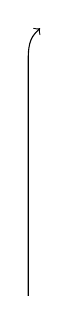
\begin{tikzpicture}[x=0.25cm,y=0.25cm]
\draw[->] (0,0)--(0,12).. controls (0,13) and (0.2,13.2)..(0.6,13.6);
\end{tikzpicture}}

D'autre part le sous-groupe de
\[
\mathcal M_{\rho,\sigma}(0)\simeq\tau_{\rho,\sigma}\subset B'_0\times T_\rho\times N'_\sigma
\]
qui opère trivialement sur $SG$, est \inserted{l'intersection de $\tau_{\rho,\sigma}$ avec} $(\deleted{\unsure{\mu_2}}\inserted{1}\times T_\rho\times N'_\sigma)$, car $B'_0$ opère \unsure{trivialt} \deleted{$\mu_2\unsure{\subset}B'_0$} (puisque
\[
(46)\qquad B'_0\cap\underbrace{\mu_2}_{\substack{\text{centre de}\\SG}}=\{1\}
\]
. C'est donc le ss-groupe des
\[
(47)\qquad
\left\{\left(1,\underset{\in\,\Gamma T_\rho}{\underline a},\underset{\in\,\Gamma N'_\sigma}{\underline b}\right)\mid(\det\underline a)^2=1,\ \det\underline b=1\right\}
\]

\margin{\unsure{non!}}
\uline{Reste} : déterminer \uline{le centre de} $\tau_{\rho,\sigma}$, extension de $\mu_2\times\mu_2$ par $\tau^0_{\rho,\sigma}\simeq\mathcal G^*_{\rho,\sigma}(0)^0\subset T_0^0\times T_\rho\times\deleted{\unsure{N'_\sigma}}\inserted{T_\sigma}$. Comme $\tau^0_{\rho,\sigma}$ est commutatif, il suffit de déterminer l'action de $\mu_2\times\mu_2$ sur $\tau^0_{\rho,\sigma}$, et d'en déterminer le sous-groupe des invariants.
\margin{Cela donnera au moins l'intersection du centre \unsure{avec} $\tau^0_{\rho,\sigma}$.}
\margin{408}
\scanpage{410}
\mspage{506}

Notons que l'on a
\[
\tau_{\rho,\sigma}=S\mathcal G^*_{\rho,\sigma}(0)\subset\mathcal G^*_{\rho,\sigma}(0)\simeq T_0\times T_\rho\times N'_\sigma
\]
et on a un hom de suites exactes

\noindent$(48)$\quad
\diagram{\begin{tikzcd}[ampersand replacement=\&,column sep=large,row sep=large]
1\arrow[r]\&\tau^0_{\rho,\sigma}\arrow[r]\arrow[d,hook]
\&\tau_{\rho,\sigma}\arrow[r,"{(\underline u,\underline a,\underline b)\mapsto(\varepsilon(\underline b),\det\underline a/\det(\underline u))}"]\arrow[d,hook]
\&\mu_2\times\mu_2\arrow[r]\arrow[d,"{\substack{\text{première}\\\text{proj}}}"]\&1\\
1\arrow[r]\&\unsure{T_0}\times T_\rho\times\deleted{\unsure{N'_\sigma}}\inserted{T_\sigma}\arrow[r]
\&T_0\times T_\rho\times N'_\sigma\arrow[r]\&\mu_2\arrow[r]\&1
\end{tikzcd}},

qui montre que l'action de $\mu_2\times\mu_2$ sur \deleted{$\unsure{\tau}$} $\tau^0_{\rho,\sigma}$ se fait par l'intermédiaire de la projection de $\mu_2\times\mu_2$ sur son premier facteur, et ce par l'opération de celui-ci sur $T_0\times T_\rho\times T_\sigma$ qui opère trivialement sur $T_0\times T_\rho$, et qui sur $T_\sigma$ est l'opération canonique de $\mu_2$ sur $T_\sigma$, $\sigma\mapsto\varepsilon\sigma$, dont les invariants sont réduits aux scalaires $\mathbb G_m$. \deleted{Donc on trouve} \inserted{Ce raisonnement} montre, plus généralement, que la \unsure{trace} \inserted{du centre de $\tau_{\rho,\sigma}$} sur le sous-groupe $\tau'_{\rho,\sigma}\subset\tau_{\rho,\sigma}$ noyau de

\diagram{\begin{tikzcd}[ampersand replacement=\&,column sep=large]
\tau_{\rho,\sigma}\arrow[r]\&\mu_2\times\mu_2\arrow[r,"{\text{1\textsuperscript{ère} proj}}"]\&\mu_2\\
(\underline u,\underline a,\underline b)\arrow[rr,mapsto]\&\&\varepsilon(\underline b)
\end{tikzcd}}

est aussi la trace, sur ce sous-groupe, de $T_0\times T_\rho\times\mathbb G_m$. D'ailleurs, comme $\mu_2$ opère \uline{fidèlement} sur $T_\sigma$ via $\sigma\mapsto\varepsilon\sigma$, on voit \deleted{que} aussitôt qu'il opère aussi fidèlement sur $\tau'_{\rho,\sigma}$ (qui en effet s'envoie \uline{\unsure{épimorphiquement}} sur $T_\sigma$ !) donc on a

\diagram{\begin{tikzcd}[ampersand replacement=\&,column sep=large]
\uline{\mathrm{Centre}}(\tau_{\rho,\sigma})\subset\tau'_{\rho,\sigma}=\operatorname{Ker}\bigl(\tau_{\rho,\sigma}
\arrow[r,"{(\underline u,\underline a,\underline b)\mapsto\varepsilon(\underline b)}"]\&\mu_2\bigr)
\end{tikzcd}}
\margin{409}
\scanpage{411}

Donc en résumé
\[
(49)\quad
\left\{
\begin{array}{l}
\uline{\mathrm{Centre}}(\mathcal G^*_{\rho,\sigma}(0))=T_0\times T_\rho\times\mathbb G_m\\[5pt]
\uline{\mathrm{Centre}}\left(\underset{S\mathcal G^*_{\rho,\sigma}(0)}{\underline{\tau_{\rho,\sigma}}}\right)
=\deleted{\unsure{\mathrm{Centre}}}(T_0\times T_\rho\times\mathbb G_m)\cap\tau_{\rho,\sigma}\\[7pt]
\hspace{7em}=\left\{\left(
\underset{\substack{\in\Gamma T_0\\\simeq\Gamma\mathbb G_m}}{\underline u},
\underset{\in\Gamma T_\rho}{\underline a},
\underset{\in\Gamma\mathbb G_m}{\unsure{\lambda}}
\right)\mid u=\lambda^2,\ \deleted{\unsure{\underline a}}\inserted{\det\underline a}=\varepsilon'\unsure{\lambda^2},\ \varepsilon'^2=1\right\}
\end{array}\right.
\]

Le sous-groupe du centre qui opère \unsure{trivialt} sur $SG$ est donc, en vertu de (47), donné par la restriction suppl. $u=1$, il s'identifie donc à \deleted{$\mu_2\times\mu_2$}
\[
(50)\quad
\left\{
\begin{array}{l}
1\times\unsure{ST'_\rho}\times\mu_2\subset\tau^{\unsure{a|0}}_{\rho,\sigma}\subset T_0\times T_\rho\times\unsure{N'_\sigma}\\[5pt]
\text{où }\unsure{ST'_\rho}\subset T_\rho\\[3pt]
\hspace{3em}\Vert\ \{\underline a\mid(\det\underline a]^2=1\}
\end{array}\right.
\]

Donc
\[
(51)\quad
\deleted{\uline{\mathrm{Centr}}(\mathcal M_{\rho,\sigma})\simeq
\left(\underset{\in T_0}{1}\times\unsure{ST'_\rho}\times\underset{\in T_\sigma}{\mu_2}\right)\times\underset{\in SG}{\mu_2}}
\]
\margin{\uline{faux} le centre est plus grand,}

Le groupe des points entiers de ce \deleted{centre}\inserted{groupe}, dans le cas modulaire, est réduit :
\[
(52)\quad
\left\{
\begin{array}{l}
\mathbb Z/6\mathbb Z\times\mathbb Z/2\mathbb Z\times\mathbb Z/2\mathbb Z\\[4pt]
\simeq\mathbb Z/3\mathbb Z\times(\mathbb Z/2\mathbb Z\times\mathbb Z/2\mathbb Z\times\mathbb Z/2\mathbb Z),
\end{array}\right.
\]
\deleted{\unsure{Groupe de}}
\margin{\uline{NB} Ce groupe est en fait contenu dans $\mathcal M^0_{\rho,\sigma}(\mathbb Z)$.}

produit d'un groupe cyclique d'ordre $3$ (engendré naturellement par $-\rho$) par un groupe $(\mathbb Z/2\mathbb Z)^3$, qui n'est autre que le groupe $\Sigma$ déjà dans (\uline{IX}).

Plus intéressant serait sans doute le
\margin{410}
\scanpage{412}
\mspage{507}

centre de $\mathcal{M}_{\rho,\sigma}^{\circ}$, qui sera donc le produit direct du centre \inserted{$\mu_2$} de $SG$ (sur lequel le groupe \inserted{\uline{commutatif}} $\mathcal{M}_{\rho,\sigma}^{\circ}(0)\simeq\tau_{\rho,\sigma}^{\circ}$ opère \unsure{trivialt}) par le ss-groupe de $\tau_{\rho,\sigma}^{\circ}\subset T_0\times T_\rho\times T_\sigma$ qui opère \unsure{trivialt} sur $SG$, savoir \deleted{$\unsure{\tau_{\rho,\sigma}}$}

\margin{\uline{faux}}

\[
\begin{aligned}
\tau_{\rho,\sigma}^{\circ}\cap 1\times T_\rho\times\unsure{T_\sigma}
 &=\{(1,\uline{a},\uline{b})\mid\det\uline{b}=1,\,
 \deleted{(}\det\uline{a}\deleted{)^{\unsure{2}}}=1\}\\
 &\simeq ST_\rho\times ST.
\end{aligned}
\]
\margin{(et pas seulement $(\det a)^2=1$, car on est dans $\tau_{\rho,\sigma}^{\circ}$}

Donc

\unsure{On}
\deleted{\diagram{\[\begin{array}{rcl}
(53)\quad\uline{\mathrm{Centre}}(\mathcal{M}_{\rho,\sigma}^{\circ})
 &=&(1\times ST_\rho\times ST_\sigma)\times\mu_2\quad,\\
 &&\hfill\cap\qquad\\[-2pt]
 &&\hfill SG\qquad
\end{array}\]}}

\margin{\uline{faux} ! Centre \unsure{est} de dim 3}

donc dans le cas modulaire on a

\deleted{\diagram{\[\begin{array}{rclccccccc}
(\unsure{54|14})\quad\uline{\mathrm{Centre}}(\mathcal{M}_{\rho,\sigma}^{\circ})(\mathbb Z)
 &\simeq&1&\times&\mathbb Z/6\mathbb Z&\times&\mathbb Z/4\mathbb Z&\times&\mathbb Z/2\mathbb Z\\
 &&&&\Vert&&\Vert&&\Vert\\
 &&&&\Gamma(ST_\rho)&&\Gamma(ST_\sigma)&&\Gamma\mu_2\subset\Gamma(SG)
\end{array}\]}}

\deleted{qui n'est que deux fois plus gros que \deleted{$\unsure{\mathcal{M}_{\rho,\sigma}}$} le groupe des pts entiers du centre de $\mathcal{M}_{\rho,\sigma}$. \deleted{(\unsure{bien que celui-ci}}}

\deleted{\uline{Rmq.} La composante neutre du centre de $\mathcal{M}_{\rho,\sigma}^{\circ}$ est bien sûr $ST_\rho\times ST_\sigma$, comme le suggérait le \unsure{dévissage|discussion} du th. p. $501'$.}

\margin{411}
\scanpage{413}
\mspage{508}

\uline{$\overline{\mathrm{XI}}$}\quad\uline{Récapitulation sur le groupe} $\mathcal{M}_{\rho,\sigma}$.

\margin{\uline{Préliminaires}}

\textcircled{$1^\circ$} Étant donné, sur un schéma $S$, une forme $G$ de $\mathrm{Gl}(2)$, d'où des formes $SG$, $PG$ de $\mathrm{Sl}(2)$, $\unsure{\mathrm{GP}(1)|\mathrm{PGl}(1)}$, et deux sections $\widetilde\rho,\widetilde\sigma$ de $PG$, et un sous-groupe à \unsure{1-paramètre} \deleted{\unsure{unipotent|multiplicatif}} additif \unsure{bordé|basé}
\diagram{\begin{tikzcd}[ampersand replacement=\&,column sep=large]
\widetilde{\uline{\varepsilon}}_0:\ G_a \arrow[r,hook] \& PG
\end{tikzcd}}
\inserted{$\unsure{\varepsilon_0|G_a}$}
(ce qui revient au $\overline{\mathrm m}$, une section \deleted{\unsure{de}} unipotente régulière \unsure{de} $\varepsilon_0$ de $G$, ou une section nilpotente régulière $N_0$ dans la forme $\mathcal M$ de $\mathrm{M}_2(\mathcal O_S)$ associée à $G$) --- satisfaisant les conditions
\[
\begin{aligned}
(1)\quad &\widetilde\sigma^{-1}\widetilde\rho
  =\widetilde{\uline{\varepsilon}}_0(1),\qquad
  \widetilde{\uline{\varepsilon}}_0\text{ et }
  \widetilde{\uline{\varepsilon}}_1
  =\rho\bigl(\widetilde{\uline{\varepsilon}}_0\bigr)
  \bigl(=\sigma\bigl(\widetilde{\uline{\varepsilon}}_0\bigr)\bigr)
  \text{ sont}\\
 &\hspace{10em}\text{indépendants sur chaque fibre}\\[4pt]
(2)\quad &\mathrm{Tr}\,\sigma=0\qquad
 \text{si }\sigma\text{ est un relèvement local de }\widetilde\sigma,
\end{aligned}
\]

On définit des relèvements \uline{canoniques} $\rho$, $\sigma$ de $\widetilde\rho,\widetilde\sigma$ à $G$, \deleted{\unsure{satisfais}} par les conditions
\[
(3)\quad\deleted{\unsure{\sigma\rho}}
\left\{\begin{array}{ll}
 \varepsilon_0=-\sigma^{-1}\rho
 &\text{i.e. }\varepsilon_1=-\rho\sigma^{-1}\\
 \mathrm{Tr}(\rho+\sigma)=1
 &\text{i.e. }\mathrm{Tr}\,\rho=1,
\end{array}\right.
\]
et les constructions qui suivent ont un sens.

On construit un \unsure{épinglage}
\diagram{\begin{tikzcd}[ampersand replacement=\&,column sep=large]
\deleted{(\unsure{4})}\ (5)\quad\deleted{\unsure{\tau_{\rho,\sigma}}=}\ \mathrm{Gl}(2)
 \arrow[r,"\sim"] \& G
\end{tikzcd}}
par la condition que $\varepsilon_1$ prenne la forme
\[
(6)\qquad\varepsilon_1
 =\begin{pmatrix}1&0\\1&1\end{pmatrix}
\]
d'où
\[
(7)\quad\left\{\begin{array}{l}
\displaystyle\rho=\begin{pmatrix}0&1\\\unsure{v|\upsilon}&1\end{pmatrix},\qquad
 \sigma=\begin{pmatrix}0&-1\\-\unsure{v|\upsilon}&0\end{pmatrix}
 \qquad(\unsure{v|\upsilon}\in\Gamma G_m\\[6pt]
\det\rho=\det\sigma=-\unsure{v|\upsilon}
\end{array}\right.
\]
\[
(8)\qquad\varepsilon_0
 =\begin{pmatrix}1&1/\unsure{v|\upsilon}\\0&1\end{pmatrix},
\]

\margin{412}
\scanpage{414}

on considère les sous-groupes
\[
(9)\quad\left\{\begin{array}{ll}
 L_0=\{\uline{\varepsilon}_0(\lambda)\}
   =\left\{\begin{pmatrix}1&\lambda\\0&1\end{pmatrix}\right\}
 & (\lambda\in\Gamma G_a)\\[7pt]
 L_1=\sigma(L_0)=\rho(L_0)
   =\{\uline{\varepsilon}_1(\lambda)\}
   =\left\{\begin{pmatrix}1&0\\\lambda&1\end{pmatrix}\right\}
 & \backslash\;\unsure{\text{id}}\\[7pt]
 B'_0=\left\{\begin{pmatrix}\mu&\lambda\\0&1\end{pmatrix}
       \mid\mu\in\Gamma G_m,\,\lambda\in\Gamma G_a\right\} &\\[7pt]
 T_0=\left\{\begin{pmatrix}\mu&0\\0&1\end{pmatrix}
       \mid\mu\in\Gamma G_m\right\} &
\end{array}\right.
\]
d'où
\[
(10)\qquad B'_0=T_0.L_0\qquad\text{(produit $\frac12$-direct)}
\]
\margin{\unsure{---}}

et on a des iso
\diagram{\[
(11)\quad\left\{\begin{gathered}
\begin{tikzcd}[ampersand replacement=\&,column sep=large,row sep=large]
\uline{\varepsilon}_0:\ G_a \arrow[r,"\sim"] \& L_0
 \&\lambda\arrow[r] \&\varepsilon_0(\lambda)
      =\begin{pmatrix}1&\lambda/\unsure{v|\upsilon}\\0&1\end{pmatrix}\\
\uline{\varepsilon}_1:\ G_a \arrow[r,"\sim"] \& L_1
 \&\lambda\arrow[r] \&\varepsilon_1(\lambda)
      =\begin{pmatrix}1&0\\\lambda&1\end{pmatrix}
\end{tikzcd}\\[5pt]
\text{donc }\uline{\varepsilon}_1(\lambda)
  =\rho\unsure{(\,|\{\,}\varepsilon_0(\lambda))
  =\sigma(\varepsilon_0(\lambda)).
\end{gathered}\right.
\]}

On \deleted{pose} considère
\[
(12)\quad\deleted{\unsure{\mathcal{G}_{\rho,\sigma}}}
\left\{\begin{aligned}
 T_\rho&=\text{schém. des unités de }\mathcal A_\rho
  =\uline{\mathcal O}_S+\uline{\mathcal O}_S\rho\\
 &\hspace{17em}\simeq\uline{\mathcal O}_S[X]/(X^2-X-\unsure{v|\upsilon})\\
 &\deleted{\text{\unsure{de}}\ \uline{\mathcal O}_S}\\
 T_\sigma&=\text{schém. des unités de }\mathcal A_\sigma
  =\uline{\mathcal O}_S+\uline{\mathcal O}_S\sigma\\
 &\hspace{17em}\simeq\uline{\mathcal O}_S[Y]/(Y^2-\unsure{v|\upsilon})
\end{aligned}\right.
\]
\diagram{\[\begin{array}{rcl}
(13)\quad &N'_\sigma&=\{g\in\Gamma G\mid g(\sigma)=\varepsilon\sigma,\ \varepsilon^2=1\}\\
 &\cap&\\[-2pt]
 &G&
\end{array}\]}
d'où
\diagram{\begin{tikzcd}[ampersand replacement=\&,column sep=large]
(14)\quad 1\arrow[r] \&T_\sigma\arrow[r] \&N'_\sigma\arrow[r,"\varepsilon_\sigma"] \&\mu_2\arrow[r] \&1.
\end{tikzcd}}

On pose
\[
(15)\quad\left\{\begin{aligned}
 \mathcal{G}_{\rho,\sigma}&=B'_0\times T_\rho\times T_\sigma\\[4pt]
 \mathcal{G}_{\rho,\sigma}^{*}&=B'_0\times T_\rho\times N'_\sigma.
\end{aligned}\right.
\]

\margin{413}
\scanpage{415}
\mspage{509}

\margin{$\begin{gathered}
 \mathcal M_{\rho,\sigma}[0],\ \mathcal M_{\rho,\sigma}(0)\,,\\
 \unsure{\tau_{\rho,\sigma}|\mathcal G_{\rho,\sigma}},\ \tau_{\rho,\sigma}^{\circ}\,,\\
 \mathcal M_{\rho,\sigma},\ \widetilde{\mathcal G}_{\rho,\sigma}^{+}\quad
   \deleted{\unsure{\mathcal M_{\rho,\sigma}^{\circ}}}\\
 \tau_{\rho,\sigma}^{\circ+}
\end{gathered}$}

\textcircled{$2^\circ$} On introduit
\[
\begin{aligned}
(16)\quad \mathcal M_{\rho,\sigma}[0]
 &\subset \unsure{\mathcal B_{\rho,\sigma}^{*}|\mathcal G_{\rho,\sigma}^{*}}
   =B'_0\times T_\rho\times N'_\sigma\\
 &\mathrel{\mathop{=}\limits^{\mathrm{dfn}}}
 \{(\uline u,\uline a,\uline b)\mid
   \det\uline u=\det\uline b=\varepsilon'\det\uline a,\
   \varepsilon'{}^2=1\}
\end{aligned}
\]
\[
(17)\qquad \mathcal M_{\rho,\sigma}(0)\subset\mathcal M_{\rho,\sigma}[0]
 \qquad\text{défini par }\uline u=1\quad\text{i.e.}
\]
\[
 \mathcal M_{\rho,\sigma}(0)=\mathcal M_{\rho,\sigma}[0]
   \cap(T_0\times T_\rho\times N'_\sigma)
 \qquad\text{dans }\mathcal G_{\rho,\sigma}^{*}.
\]
\diagram{\begin{tikzcd}[ampersand replacement=\&,column sep=large,row sep=small]
(18)\quad L_0\arrow[r,hook] \&\mathcal M_{\rho,\sigma}[0]\\
\lambda\arrow[r,mapsto] \&(\lambda,1,1)
\end{tikzcd}}
donc on a
\[
(19)\qquad \mathcal M_{\rho,\sigma}[0]\simeq
  \mathcal M_{\rho,\sigma}\unsure{[0)|(0)}\, .\, L_0
 \qquad\text{produit }\tfrac12\text{-direct}
\]

On a un homomorphisme
\diagram{\begin{tikzcd}[ampersand replacement=\&,column sep=huge]
(20)\quad\unsure{\dot{\mathcal M}|\mathcal M}_{\rho,\sigma}[0]\arrow[r]
 \&G_m\times\mu_2\times\mu_2
\end{tikzcd}}
\[
 \text{noté }\{g\mapsto\chi(g),\varepsilon_2(g),\varepsilon_3(g)
\]
pour $g=(\uline u,\uline a,\uline b)$ on a
\[
\begin{aligned}
 \chi(g)&=\det\uline u=\det\uline b\\
 \varepsilon_2(g)&=\varepsilon_\sigma(b)\qquad\text{(cf (13)(14)}\\
 \varepsilon_3(g)&=\det(\uline a)/\det\uline b\\
 &\text{i.e. }\left\{\begin{array}{l}
    \det a=\varepsilon_3\mu\\
    \text{où }\mu=\chi(g)
  \end{array}\right.
\end{aligned}
\]
trivial sur $L_0$ (donc se factorisant par le quotient). On pose aussi
\[
(21)\qquad\tau_{\rho,\sigma}\simeq\mathcal M_{\rho,\sigma}[0]/L_0
 \qquad\text{\unsure{où}}
\]
\margin{Cette notation n'est pas du tout adéquate (\unsure{inspirée à tort} du $\tau_{g,\unsure{\nu|r}}$) \unsure{la suite montre} (et ce qui précède montrait déjà) que la notation $\Gamma_{\rho,\sigma}$ conviendrait, inspirée par $\Gamma_{g,\nu}$ et $\Gamma_{0,3}$.}

\unsure{et} le composé
\diagram{\begin{tikzcd}[ampersand replacement=\&,column sep=large]
(22)\quad\mathcal M_{\rho,\sigma}(0)\arrow[r,hook]
 \&\mathcal M_{\rho,\sigma}[0]\arrow[r] \&\tau_{\rho,\sigma}
\end{tikzcd}}
est un \uline{iso}, d'où on a
\diagram{\begin{tikzcd}[ampersand replacement=\&,column sep=large]
(23)\quad\unsure{\mathcal M|\mathcal G}_{\rho,\sigma}(0)
 \simeq\unsure{\tau_{\rho,\sigma}|\tau_{\rho,\sigma}'}\arrow[r,hook]
 \&T_0\times T_\rho\times N'_\sigma
\end{tikzcd}}

\margin{414}
% ===== LM_C3-416-434: second pass, checked against the scans =====
\scanpage{416}

La composition avec la projection can. dans
$T_\rho\times N'_\sigma$ donne un \uline{mono}

\margin{car on aura
\diagram{\begin{tikzcd}[ampersand replacement=\&]
T_0 \arrow[r,"{\substack{\det\\\sim}}"] \& \mathbb G_m
\end{tikzcd}}}

\[
(24)\qquad
\diagram{\begin{tikzcd}[ampersand replacement=\&,column sep=large]
\mathcal T_{\rho,\sigma} \arrow[r,hook] \arrow[d,phantom,"{\rotatebox{90}{$\simeq$}}" description]
 \& T_\rho\times N'_\sigma \\
\left\{(\underline a,\underline b)\mid
 (\det\underline a/\det\underline b)^2=1\right\}
 \& \inserted{\left.\begin{gathered}
\text{i.e. }\det\underline a=\varepsilon'\det\underline b\\
\text{avec }\varepsilon'^2=1
\end{gathered}\right\}}
\end{tikzcd}}
\]

et on aura donc
\[
(25)\qquad
\left\{\begin{aligned}
\chi(\underline a,\underline b)&=\det\underline b\\
\varepsilon_2(\underline a,\underline b)&=\varepsilon_\sigma(\underline b)\\
\varepsilon_3(\underline a,\underline b)&=\det(\underline a)/\det(\underline b)
 =\det\underline b/\det\underline a
\end{aligned}\right.
\]

On définit
\[
(26)\qquad
\diagram{\begin{tikzcd}[ampersand replacement=\&,column sep=small]
\mathcal T_{\rho,\sigma}^{\circ} \arrow[d,phantom,"{\rotatebox{90}{$\simeq$}}" description]
 \& {}=\operatorname{Ker}\mathcal T_{\rho,\sigma}
 \arrow[r,"{(\varepsilon_2,\varepsilon_3)}"]
 \& \mu_2\times\mu_2 \\
\inserted{T_\rho\times_{\mathbb G_m}T_\sigma} \&\&
\end{tikzcd}}
\]
donc on a
\[
(27)\qquad
\diagram{\begin{tikzcd}[ampersand replacement=\&]
1 \arrow[r] \& \mathcal T_{\rho,\sigma}^{\circ} \arrow[r]
 \& \mathcal T_{\rho,\sigma} \arrow[r] \& \mu_2\times\mu_2 \arrow[r] \& 1
\end{tikzcd}}
\]
et une suite exacte canonique
\[
(28)\qquad
\diagram{\begin{tikzcd}[ampersand replacement=\&]
1 \arrow[r] \&
\overbrace{ST_\rho\times ST_\sigma}^{\inserted{\mathcal T_{\rho,\sigma}^{\circ+}}}
\arrow[r] \& \mathcal T_{\rho,\sigma}^{\circ} \arrow[r,"{\chi}"]
 \& \mathbb G_m \arrow[r] \& 1,
\end{tikzcd}}
\]
où on définit
\[
(29)\qquad
\left\{\begin{aligned}
ST_\rho&=\{g\in\Gamma T_\rho\mid\det g=1\}\\
ST_\sigma&=\{g\in\Gamma T_\sigma\mid\det g=1\}
\end{aligned}\right.\quad.
\]

\margin{\figure{\begin{tikzpicture}[x=.65cm,y=.65cm]
\draw[->] (0,4.5) .. controls (1.1,4.55) and (1.1,3.7) .. (1.1,3.25)
 -- (1.2,.8) .. controls (1.2,.45) and (1.55,.55) .. (2.4,.65);
\draw (0,0) .. controls (1.0,-.05) and (1.05,.1) .. (1.15,.45)
 .. controls (1.25,.75) and (1.55,.65) .. (2.4,.65);
\end{tikzpicture}}}
\inserted{L'opération de $\mathcal T_{\rho,\sigma}\simeq
\mathcal M_{\rho,\sigma}(0)$ sur $L_0$ est donnée par
\[
(30)\qquad g(\varepsilon_0(\lambda))=\varepsilon_0(\mu\lambda),
\quad\text{où }\mu=\chi(g)
\]}

On fait opérer $\mathcal M_{\rho,\sigma}(0)
(\simeq\mathcal T_{\rho,\sigma})$ sur $SG$, par
\[
(31)\qquad
\diagram{\begin{tikzcd}[ampersand replacement=\&,column sep=large]
\mathcal M_{\rho,\sigma}(0)
 \arrow[r,"{\text{projection}}"]
 \& T_0 \arrow[r,"{\substack{\text{can.}\\(\text{mono})}}"]
 \& PG \arrow[r,"{\sim}"]
 \& \underline{\operatorname{Aut}}_{\mathrm{gr}}(SG) \\
T_0\times T_\rho\times N'_\sigma \arrow[u,phantom,"{\cap}" description]
 \& G \arrow[u,phantom,"{\cap}" description]
 \& G/\mathbb G_m\simeq\underline{\operatorname{Aut}}(G)
 \arrow[u,phantom,"{\rotatebox{90}{$\simeq$}}" description] \&
\end{tikzcd}}
\]

\par\noindent 415
\scanpage{417}
\mspage{510}

et on définit
\[
(32)\qquad \mathcal M_{\rho,\sigma}\simeq
 \mathcal M_{\rho,\sigma}(0)\mathbin{.}SG
\]
\hfill produit $\frac12$ direct

On a donc un hom can
\[
(33)\qquad
\diagram{\begin{tikzcd}[ampersand replacement=\&]
SG \arrow[r,hook,"{j}"] \& \mathcal M_{\rho,\sigma}
\end{tikzcd}}
\]
dont l'image est notée $\widetilde{\mathcal G}_{\rho,\sigma}^{+}$, donc
\[
(34)\qquad
\diagram{\begin{tikzcd}[ampersand replacement=\&]
1 \arrow[r] \& \widetilde{\mathcal G}_{\rho,\sigma}^{+} \arrow[r]
 \& \mathcal M_{\rho,\sigma} \arrow[r] \& \mathcal T_{\rho,\sigma} \arrow[r] \& 1
\end{tikzcd}}
\]
\[
(35)\qquad
\diagram{\begin{tikzcd}[ampersand replacement=\&,column sep=0.3em,row sep=1.3em]
\mathcal M_{\rho,\sigma}\simeq \& \mathcal M_{\rho,\sigma}(0)
 \arrow[d,phantom,"{\rotatebox{90}{$\simeq$}}" description]
 \& {}\mathbin{.}\widetilde{\mathcal G}_{\rho,\sigma}^{+} \\
 \& \mathcal T_{\rho,\sigma} \&
\end{tikzcd}}
\]
\hfill produit $\frac12$ direct.

\uline{NB.} On utilise la notation $\mathcal T_{\rho,\sigma}$ pour le
groupe quotient
\[
(36)\qquad \mathcal T_{\rho,\sigma}\simeq
\mathcal M_{\rho,\sigma}/\widetilde{\mathcal G}_{\rho,\sigma}^{+},
\]
la notation $\mathcal M_{\rho,\sigma}[0)$ pour le sous-groupe
de $\mathcal M_{\rho,\sigma}$.

On définit un plongement canonique
\[
(37)\qquad
\diagram{\begin{tikzcd}[ampersand replacement=\&]
\mathcal M_{\rho,\sigma}[0] \arrow[r,hook,"{i}"] \& \mathcal M_{\rho,\sigma}
\end{tikzcd}}
\]
qui prolonge les inclusions \unsure{des sous-groupes|du sous-groupe}
$\mathcal M_{\rho,\sigma}(0)$ commun de $\mathcal M_{\rho,\sigma}[0]$
et de $\mathcal M_{\rho,\sigma}$,
et qui sur $L_0$ est donné par
\[
(38)\qquad i(\lambda)=j(\lambda)\qquad (\text{cf }(33))
\]
(ce qui est bien compatible avec les opérations de
$\deleted{\unsure{\mathcal T|\mathcal M}}\mathcal M_{\rho,\sigma}(0)$
sur $L_0$ d'une part, sur $SG\simeq\widetilde{\mathcal G}_{\rho,\sigma}^{+}$
de l'autre).

\par\noindent 416
\scanpage{418}

Une autre façon de le dire, c'est de constater que
$\mathcal M_{\rho,\sigma}(0)$ opérant sur
$SG\simeq\widetilde{\mathcal G}_{\rho,\sigma}^{+}$
normalise le sous-groupe $j(L_0)$ -- que nous
identifions désormais à $L_0$), de sorte qu'on
aura un sous-groupe
\[
\mathcal M_{\rho,\sigma}(0)\mathbin{.}L_0\subset\mathcal M_{\rho,\sigma}
\]
qui \unsure{est|sera} canoniquement isom. à $\mathcal M_{\rho,\sigma}[0]$
défini plus haut, grâce à l'écriture $(\unsure{19|49})$ de
celui-ci comme produit $\frac12$-direct.

\deleted{\uline{Proposition}}
\inserted{\uline{Remarque.}} On a
\[
\deleted{(\unsure{39})}\qquad
\mathcal M_{\rho,\sigma}[0]\subset
\underline{\operatorname{Norm}}_{\mathcal M_{\rho,\sigma}}(L_0)
\]

Par construction, \deleted{\unsure{on a} $\subset$, \unsure{pour} $\unsure{\supset}$}
l'inclusion en sens inverse reviendrait à dire que $L_0$
est son propre normalisateur dans $SG\simeq\widetilde{\mathcal G}_{\rho,\sigma}^{+}$,
ce qui bien sûr n'est pas vrai du tout
-- \unsure{bien} que le fait analogue soit vrai
dans le groupe profini
$\widetilde{\mathcal G}_{0,3}^{\widehat{+}}$,
pour le ss-groupe engendré par $\varepsilon_0$,
ou dans $\Pi_{0,\widehat{3}}$ pour
celui engendré par $l_0$ (\unsure{moyennant} vérification !
d'ailleurs que je n'ai tjrs pas fait).

\par\noindent 417
\scanpage{419}
\mspage{511}

\margin{$\mathcal M_{\rho,\sigma}^{\circ},\mathcal M_{\rho,\sigma}^{+},
\mathcal M_{\rho,\sigma}^{+\circ},\mathcal T_{\rho,\sigma}^{\circ},
\mathcal T_{\rho,\sigma}^{+},\mathcal T_{\rho,\sigma}^{\circ+}\ldots$
quelques sous-groupes centraux et calculs de \unsure{pts} entiers\ldots}

\figure{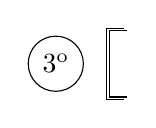
\begin{tikzpicture}[baseline=(n.base)]
\node[draw,circle,inner sep=3pt] (n) at (0,0) {$3^{\mathrm o}$};
\draw[line width=.6pt] (.90,.42)--(.68,.42)--(.68,-.42)--(.90,-.42);
\draw[line width=.45pt] (.86,.45)--(.64,.45)--(.64,-.45)--(.86,-.45);
\end{tikzpicture}}
On désigne par $\mathcal M_{\rho,\sigma}^{\circ}$,
$\mathcal M_{\rho,\sigma}[0]^{\circ}$,
$\deleted{\unsure{\mathcal M}}\mathcal M_{\rho,\sigma}[0)^{\circ}$
composantes neutres, on aura p.ex
\[
(39)\qquad
\diagram{\begin{tikzcd}[ampersand replacement=\&,column sep=small]
1 \arrow[r] \& \mathcal M_{\rho,\sigma}^{\circ}
 \arrow[r] \arrow[d,phantom,"{\rotatebox{90}{$\simeq$}}" description]
 \& \mathcal M_{\rho,\sigma} \arrow[r] \& \mu_2\times\mu_2 \arrow[r] \& 1\\
 \& \mathcal M_{\rho,\sigma}^{\circ}(0)\mathbin{.}\widetilde{\mathcal G}_{\rho,\sigma}^{+}
 \&\&\&
\end{tikzcd}}
\]
\hspace*{4em} produit $\frac12$ direct
\[
(40)\qquad
\diagram{\begin{tikzcd}[ampersand replacement=\&]
\mathcal M_{\rho,\sigma}(0)^{\circ} \arrow[r,"{\sim}"]
 \& \mathcal T_{\rho,\sigma}^{\circ}\simeq T_\rho\times_{\mathbb G_m}T_\sigma
\end{tikzcd}}
\]
\[
(41)\qquad
\begin{gathered}
\mathcal M_{\rho,\sigma}^{\circ}\text{ est l'image inverse de }
\mathcal T_{\rho,\sigma}^{\circ}\\
\text{par }\diagram{\begin{tikzcd}[ampersand replacement=\&]
\mathcal M_{\rho,\sigma} \arrow[r,"{\text{can}}"] \& \mathcal T_{\rho,\sigma}
\end{tikzcd}},
\end{gathered}
\]

on a un hom canonique composé
\[
(42)\qquad
\diagram{\begin{tikzcd}[ampersand replacement=\&]
\mathcal M_{\rho,\sigma} \arrow[r] \& \mathcal T_{\rho,\sigma}
 \arrow[r,"{\chi}"] \& \mathbb G_m
\end{tikzcd}}
\]
également noté $\chi$, son noyau est noté
$\mathcal M_{\rho,\sigma}^{+}$, et on définit de $=$
$\mathcal M_{\rho,\sigma}^{\circ+}$, donc
\[
(43)\qquad
\diagram{\begin{tikzcd}[ampersand replacement=\&]
1 \arrow[r] \& \mathcal M_{\rho,\sigma}^{+} \arrow[r]
 \arrow[d,phantom,"{\unsure{\cup|\downarrow}}" description]
 \& \mathcal M_{\rho,\sigma} \arrow[r,"{\chi}"]
 \arrow[d,phantom,"{\unsure{\cup|\downarrow}}" description]
 \& \mathbb G_m \arrow[r]
 \arrow[d,phantom,"{\unsure{\cup|\downarrow}}" description] \& 1\\
1 \arrow[r] \& \mathcal M_{\rho,\sigma}^{\circ+} \arrow[r]
 \& \mathcal M_{\rho,\sigma}^{\circ} \arrow[r,"{\chi}"]
 \& \mathbb G_m \arrow[r] \& 1
\end{tikzcd}}
\]
\[
(44)\qquad
\left\{\begin{aligned}
\mathcal M_{\rho,\sigma}^{+}&\simeq
\underbrace{\mathcal M_{\rho,\sigma}^{+}(0)}_{
\substack{\rotatebox{90}{$\simeq$}\\\mathcal T_{\rho,\sigma}^{+}}}
\mathbin{.}\widetilde{\mathcal G}_{\rho,\sigma}^{+}\\[3em]
\mathcal M_{\rho,\sigma}^{\circ+}&\simeq
\underbrace{\mathcal M_{\rho,\sigma}^{\circ+}(0)}_{
\substack{\rotatebox{90}{$\simeq$}\\
\mathcal T_{\rho,\sigma}^{\circ+}\simeq ST_\rho\times ST_\sigma\\
\text{cf }(28)}}
\mathbin{.}\widetilde{\mathcal G}_{\rho,\sigma}^{+}
\end{aligned}\right.
\]

Donc on a
\[
(45)\qquad
\begin{gathered}
\mathcal M_{\rho,\sigma}^{\circ+}(0)\overset{\mathrm{dfn}}=
\operatorname{Ker}\left(\diagram{\begin{tikzcd}[ampersand replacement=\&]
\mathcal M_{\rho,\sigma}^{\circ}(0)
 \arrow[r,"{{\chi,\varepsilon_2,\varepsilon_3}}"]
 \& \mathbb G_m\times\mu_2\times\mu_2
\end{tikzcd}}\right)\\
\simeq ST_\rho\times ST_\sigma
\end{gathered}
\]
et ce sous-groupe est \uline{central} dans
$\mathcal M_{\rho,\sigma}^{\circ}$
(pas dans $\mathcal M_{\rho,\sigma}$), de façon précise

\par\noindent 418
\scanpage{420}

on a
\[
\begin{aligned}
(46)\qquad
\mathcal M_{\rho,\sigma}^{\circ+}
&\overset{\mathrm{dfn}}{=}
\operatorname{Ker}\bigl(\mathcal M_{\rho,\sigma}
\xrightarrow{(\chi,\varepsilon_2,\varepsilon_3)}
\mathbb G_m\times\mu_2\times\mu_2\bigr)
\deleted{\unsure{\simeq}}\\
&\simeq
\underbrace{ST_\rho\times ST_\sigma}_{\subset\mathcal M_{\rho,\sigma}(0)}
\times\widetilde{\mathcal G}_{\rho,\sigma}^{+}
\end{aligned}
\]

\margin{Toute la fin du n° devrait venir
après (ou avant) \unsure{le} n° $6^\circ$
\unsure{à propos} des ``\unsure{radicalités}''}

\margin{$\circ$ Attention, cette inclusion n'est pas une égalité,
cf plus bas\ldots}

\[
(47)\qquad
\uline{\operatorname{Centr}}(\mathcal M_{\rho,\sigma}^{\circ})
\supset
\underbrace{1\times ST_\rho\times ST_\sigma}_{\substack{\cap\\
\mathcal M_{\rho,\sigma}(0)^\circ}}
\times
\underset{\substack{\cap\\\widetilde{\mathcal G}_{\rho,\sigma}^{+}\simeq SG}}{\mu_2}.
\]

D'où un sous-groupe
\[
(48)\qquad
\mu_2\times\mu_2\times\mu_2
\subset 1\times
\underbrace{ST_\rho\times ST_\sigma\times\mu_2}_{\substack{\cap\\
\operatorname{Centr}(\mathcal M_{\rho,\sigma}^{\circ})}}
\]
qui est en fait contenu dans le Centre de $\mathcal M_{\rho,\sigma}$
tout entier, car
\[
(49)\qquad
\uline{\operatorname{Centr}}(\mathcal M_{\rho,\sigma})
\supset
\underbrace{1\times S'T_\rho\times\mu_2}_{\substack{\cap\\
\mathcal M_{\rho,\sigma}(0)}}
\times
\underset{\substack{\cap\\\widetilde{\mathcal G}_{\rho,\sigma}^{+}\simeq SG}}{\mu_2}
\]
\margin{\unsure{id.}}
avec
\[
(50)\qquad
S'T_\rho\overset{\mathrm{dfn}}{=}
\{g\in\Gamma T_\rho\mid(\det g)^2=1\}
\]
de sorte qu'on a
\diagram{\begin{tikzcd}[ampersand replacement=\&,column sep=large]
\text{(51)}\quad 1 \arrow[r] \& ST_\rho \arrow[r] \&
S'T_\rho \arrow[r,"{\varepsilon_3}"] \& \mu_2 \arrow[r] \& 1
\end{tikzcd}}

On a donc
\[
(52)\qquad
\operatorname{Centr}(\mathcal M_{\rho,\sigma})\cap
\mathcal M_{\rho,\sigma}^{\circ}
\supset
\underset{\substack{\cap\\T_0}}{1}\times
\underset{\substack{\cap\\T_\rho}}{ST_\rho}\times
\underset{\substack{\cap\\T_\sigma}}{\mu_2}\times
\underset{\substack{\cap\\\widetilde{\mathcal G}_{\rho,\sigma}^{+}}}{\mu_2}.
\]
\margin{\unsure{id.}}

Le ``cas modulaire'' est celui où
\[
(53)\qquad
\left\{\begin{aligned}
\det\rho&=1\quad\text{i.e.}\quad\det\sigma=1
\quad\text{i.e.}\quad\nu=-1\\
\text{i.e.}\quad\rho&=\begin{pmatrix}0&1\\-1&1\end{pmatrix}
\quad\text{i.e.}\quad\sigma=\begin{pmatrix}0&1\\-1&0\end{pmatrix}
\end{aligned}\right.
\]
(cf \uline{$\overline{\mathrm{VI}}$} pour d'autres
caractérisations, telles
$\sigma^2=-1$, ou $\rho^2-\rho+1=0$, ou
$\widetilde\sigma^2=\widetilde\rho^3=1\ldots$),
cela signifie aussi que $\rho$ (en tant qu'élément de $T_\rho$)
est dans $ST_\rho$ donc dans le \unsure{centr.} de $\mathcal M_{\rho,\sigma}^{\circ}$,

\par\noindent 419
\scanpage{421}
\mspage{512}

ou que $\sigma$ en tant qu'élément de $T_\sigma$
est dans $ST_\sigma$ i.e. dans le centre de $\mathcal M_{\rho,\sigma}^{\circ}$.
Donc dans ce cas on trouve un homomorphisme
\diagram{\(\displaystyle
(54)\quad\left\{
\begin{gathered}
\begin{tikzcd}[ampersand replacement=\&,column sep=large,row sep=large]
\mathbb Z/6\mathbb Z\times\mathbb Z/4\mathbb Z \arrow[r] \&
\uline{\operatorname{Centr}}(\mathcal M_{\rho,\sigma}^{\circ})\\
(i,j) \arrow[r] \& i_\rho(\rho^i)i_\sigma(\sigma^j)
\end{tikzcd}
\end{gathered}\right.
\)}
(où on définit $i_\rho,i_\sigma$ parmi les
\deleted{\unsure{quatre}}\inserted{trois} morphismes canoniques
\[
\deleted{(55)\quad\unsure{i_B}:B'_0\longrightarrow
\mathcal M_{\rho,\sigma}[0]\subset\mathcal M_{\rho,\sigma}}
\]
\diagram{\(\displaystyle
(55)\quad\left\{
\begin{gathered}
\begin{tikzcd}[ampersand replacement=\&,column sep=large,row sep=small]
i_\rho:S'T_\rho \arrow[r] \& \mathcal M_{\rho,\sigma}(0)
\arrow[r,phantom,"{\subset}" description] \& \mathcal M_{\rho,\sigma}\\
i_\sigma:\unsure{SN'_\sigma} \arrow[r] \& \mathcal M_{\rho,\sigma}(0)
\arrow[r,phantom,"{\subset}" description] \& \mathcal M_{\rho,\sigma}\\
i_G:SG\simeq\widetilde{\mathcal G}_{\rho,\sigma}^{+}
\arrow[r] \& \mathcal M_{\rho,\sigma}, \&
\end{tikzcd}
\end{gathered}\right.\qquad)
\)}
dont l'image, pour $2$ inversible sur $S$, contient
contient l'image de $\mu_2\times\mu_2\times1$ dans (48).
Pour $2$ inv. sur $S$, l'hom (53) est un mono
(mais pas en car. $2$, bien sûr). Sur la base absolue $\mathbb Z$,
on a par ailleurs, dans le cas modulaire
\[
(56)\qquad
\left\{\begin{aligned}
\mathcal T_{\rho,\sigma}(\mathbb Z)&\simeq
T_\rho(\mathbb Z)\times N'_\sigma(\mathbb Z)
\simeq\mathbb Z/6\mathbb Z\times\mathbb D_4\\
\mathcal M_{\rho,\sigma}(\mathbb Z)&\simeq
\mathcal T_{\rho,\sigma}(\mathbb Z)\mathbin{.}\operatorname{Sl}(2,\mathbb Z)
\end{aligned}\right.
\]
\inserted{produit $\frac12$ direct,
$\unsure{\mathbb D|\mathcal B|\mathcal T}_{\rho,\sigma}\simeq
\mathbb Z/6\mathbb Z\times\mathbb D_4$ opérant via le caractère
\diagram{\begin{tikzcd}[ampersand replacement=\&,column sep=large]
\mathbb D_4 \arrow[r,"{\varepsilon_2}"] \&
\mathbb Z/2\mathbb Z\simeq\unsure{(1,\tau_\infty)|\{1,\tau_\infty\}}
\end{tikzcd}}
$\tau_\infty$ opérant sur $\operatorname{Sl}(2,\mathbb Z)$ par
autom. induit par la matrice
\[
\tau_\infty=\begin{pmatrix}-1&0\\0&1\end{pmatrix}
\]
}

\margin{\figure{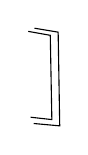
\begin{tikzpicture}[x=1cm,y=1cm]
\draw (0,1.15)--(.28,1.10)--(.30,.03)--(.03,.06);
\draw (.08,1.19)--(.38,1.14)--(.40,-.05)--(.07,-.02);
\end{tikzpicture}}}

\par\noindent 420
\scanpage{422}

\margin{les hom $\Theta,\widetilde\Theta$
$\Theta^\circ,\widetilde\Theta^\circ$}

\textcircled{\(4^\circ\)}\quad On définit un hom.
\diagram{\begin{tikzcd}[ampersand replacement=\&,column sep=huge]
\text{(57)}\quad\mathcal M_{\rho,\sigma} \arrow[r,"{\Theta}"] \& G
\end{tikzcd}}
\[
\Theta\mid\widetilde{\mathcal G}_{\rho,\sigma}^{+}\simeq SG
\quad\text{est l'identité}
\]
\[
\Theta\mid\mathcal M_{\rho,\sigma}(0)\subset
T_0\times T_\rho\times N'_\sigma
\quad\text{donné par}\quad
\Theta(\underline u,\underline a,\underline b)=\underline u
\]
d'où
\[
(58)\qquad
\Theta\mid\mathcal M_{\rho,\sigma}[0]\subset
B'_0\times T_\rho\times N'_\sigma
\quad\text{donné par}\quad
\Theta(\underline u,\underline a,\underline b)=\underline u
\]

On a
\diagram{\begin{tikzcd}[ampersand replacement=\&,column sep=large,row sep=large]
\text{(59)}\quad\deleted{\operatorname{Ker}\Theta=}
\arrow[d,phantom,"{\deleted{\simeq}}"{description,rotate=90}]
\& \mathcal M_{\rho,\sigma}(0)
\arrow[r,phantom,"{\subset}" description]
\arrow[d,phantom,"{\cup}" description]
\arrow[dr,phantom,"{\text{cart.}}" description]
\& T_0\times T_\rho\times N'_\sigma
\arrow[d,phantom,"{\cup}" description]\\
\deleted{\unsure{\mathcal R|SG}}
\& \operatorname{Ker}\Theta
\arrow[r,phantom,"{\subset}" description]
\& 1\times T_\rho\times N'_\sigma
\end{tikzcd}}
\[
\begin{gathered}
\rotatebox{90}{$\simeq$}\quad
\left\{\left(1,
\underset{\substack{\rotatebox{90}{$\in$}\\\Gamma T_\rho}}{\underline a},
\underset{\substack{\rotatebox{90}{$\in$}\\\Gamma N'_\sigma}}{\underline b}
\right)\,\middle|\,\det\underline b=1,(\det\underline a)^2=1\right\}\\
\rotatebox{90}{$\simeq$}\quad S'T_\rho\times SN'_\sigma
\end{gathered}
\]
\inserted{où
$SN'_\sigma=\operatorname{Ker}(N'_\sigma\xrightarrow{\text{dét}}\mathbb G_m)$}

Soit
\[
(60)\qquad
\Theta^\circ=\Theta\mid\mathcal M_{\rho,\sigma}^{\circ}
\qquad\deleted{\text{\unsure{qu'on|on a}}}
\]
on trouve
\diagram{\begin{tikzcd}[ampersand replacement=\&,column sep=large,row sep=small]
\text{(61)}\quad1 \arrow[r] \& \operatorname{Ker}\Theta^\circ
\arrow[r] \arrow[d,phantom,"{\simeq}"{description,rotate=90}]
\& \operatorname{Ker}\Theta \arrow[r,"{(\varepsilon_3,\varepsilon_2)}"]
\& \mu_2\times\mu_2 \arrow[r] \& 1.\\
\& ST_\rho\times ST_\sigma
\arrow[d,phantom,"{\deleted{\simeq}}"{description,rotate=90}] \& \& \&\\
\& \deleted{\operatorname{Centr}} \& \& \&\\[-1.5ex]
\& \deleted{\bigl(\uline{\operatorname{Rad}}(\mathcal M_{\rho,\sigma}^{\circ})}
\arrow[d,phantom,"{\deleted{\simeq}}"{description,rotate=90}] \& \& \&\\
\& \deleted{\uline{\operatorname{Centr}}^\circ(\mathcal M_{\rho,\sigma}^{\circ})\bigr)}
\& \& \&
\end{tikzcd}}

Posons
\[
(62)\qquad
S\mathcal R_{\rho,\sigma}^{\circ}
=1\times ST_\rho\times ST_\sigma
=\operatorname{Ker}\Theta^\circ
=(\operatorname{Ker}\Theta)\cap\mathcal M_{\rho,\sigma}^{\circ}
\]
qui est un sous-groupe central de $\mathcal M_{\rho,\sigma}^{\circ}$
(il est

\par\noindent 421
\scanpage{423}
\mspage{513}

\deleted{\unsure{invariant}}\inserted{distingué}
mais pas central dans $\mathcal M_{\rho,\sigma}$ tout entier)

le groupe
\[
(63)\qquad
\mathcal M_{\rho,\sigma}/S\mathcal R_{\rho,\sigma}^{\circ}
=\mathcal M_{\rho,\sigma}^{\unsure{\natural}}
\]
est donc une extension de $\mu_2\times\mu_2$ par
\[
\mathcal M_{\rho,\sigma}^{\circ}/S\mathcal R_{\rho,\sigma}^{\circ}
\overset{\mathrm{dfn}}{=}
\mathcal M_{\rho,\sigma}^{\circ\unsure{\natural}},
\]
isomorphe à $G$ par $\Theta^\circ$
(puisque $S\mathcal R_{\rho,\sigma}^{\circ}=\operatorname{Ker}\Theta^\circ$), donc
\diagram{\begin{tikzcd}[ampersand replacement=\&,column sep=large]
\text{(64)}\quad1 \arrow[r] \& G \arrow[r] \&
\mathcal M_{\rho,\sigma}^{\unsure{\natural}} \arrow[r] \&
\mu_2\times\mu_2 \arrow[r] \& 1,
\end{tikzcd}}
d'ailleurs l'hom
\diagram{\begin{tikzcd}[ampersand replacement=\&,column sep=large]
\Theta:\mathcal M_{\rho,\sigma} \arrow[r] \& G
\end{tikzcd}}
étant trivial sur $\mathcal R_{\rho,\sigma}$ passe au quotient en
\diagram{\begin{tikzcd}[ampersand replacement=\&,column sep=large]
\text{(65)}\quad\Theta^{\unsure{\natural}}:
\mathcal M_{\rho,\sigma}^{\unsure{\natural}} \arrow[r] \& G,
\end{tikzcd}}
\unsure{dont} la restriction à $G$ (via (64)) est l'identité,
donc on trouve, via (64),
\[
(66)\qquad
\mathcal M_{\rho,\sigma}^{\unsure{\natural}}\simeq
G\times\mu_2\times\mu_2.
\]
On trouve donc
\diagram{\begin{tikzcd}[ampersand replacement=\&,column sep=large,row sep=small]
\text{(67)}\quad1 \arrow[r] \& S\mathcal R_{\rho,\sigma}^{\circ}
\arrow[r] \arrow[d,phantom,"{\simeq}"{description,rotate=90}]
\& \mathcal M_{\rho,\sigma}
\arrow[r,"{(\Theta,\varepsilon_3,\varepsilon_2)}"] \&
\mathcal M_{\rho,\sigma}^{\unsure{\natural}}
\arrow[r] \arrow[d,phantom,"{\simeq}"{description,rotate=90}] \& 1.\\
\& ST_\rho\times ST_\sigma \& \& G\times\mu_2\times\mu_2 \&
\end{tikzcd}}

Pour voir comment
$\mathcal M_{\rho,\sigma}^{\unsure{\natural}}\simeq G\times\mu_2\times\mu_2$
opère sur $ST_\rho\times ST_\sigma$, on
\deleted{considère le}\inserted{note que}\deleted{l'image}
$\mathcal M_{\rho,\sigma}^{\circ}$ est l'image inverse de
$G\simeq\mathcal M_{\rho,\sigma}^{\unsure{\natural}\circ}$
\deleted{sous-groupe}
dans l'extension (67), où $S\mathcal R_{\rho,\sigma}$ est central
dans $\mathcal M_{\rho,\sigma}$, donc $G$ y opère trivialement.

\par\noindent 422
\scanpage{424}

D'autre part on a
\diagram{\begin{tikzcd}[ampersand replacement=\&,column sep=large,row sep=small]
S\mathcal R_{\rho,\sigma}^{\circ}
\arrow[r,phantom,"{\subset}"{description}]
\arrow[d,phantom,"{\simeq}"{description,rotate=90}]
\& \mathcal M_{\rho,\sigma}(0)
\arrow[r,"{\text{épi}}","{(\varepsilon_3,\varepsilon_2)}"']
\arrow[d,phantom,"{\cap}"{description}]
\& \mu_2\times\mu_2\\
ST_\rho\times ST_\sigma \& T_0\times T_\rho\times N'_\sigma \&
\end{tikzcd}}
et on trouve que $\mu_2\times\mu_2$ opère sur
$S\mathcal R_{\rho,\sigma}$ via son deuxième facteur
(correspondant à
$\varepsilon_2(\underline u,\underline a,\underline b)
=\varepsilon_\sigma(\underline b)$), un $\varepsilon$ de celui-ci
($\varepsilon^2=1$) opère sur
$S\mathcal R_{\rho,\sigma}\simeq ST_\rho\times ST_\sigma$
en laissant intouché le premier facteur,
et en opérant sur $T_\sigma$ donc sur $ST_\sigma$ via
\diagram{\begin{tikzcd}[ampersand replacement=\&,column sep=large]
\text{(68)}\qquad\sigma \arrow[r] \& \varepsilon\sigma
\end{tikzcd}}
\margin{(compatible avec l'équation de Hamilton--Cayley
$\sigma^2-\nu=0$ de $\sigma$)}

\deleted{On trouve en passant que l'image inverse
 dans $\mathcal M_{\rho,\sigma}$
\inserted{(ou $\mathcal M_{\rho,\sigma}^{\circ}$)}
du sous-groupe $\mathbb G_m\subset G$
centre de $G$ \unsure{n'est autre que}
$\mathcal M_{\rho,\sigma}^{\unsure{\circ}}(0)^\circ$.}

\textcircled{\(5^\circ\)}\quad Soit
\[
(69)\qquad
\begin{gathered}
\mathcal R_{\rho,\sigma}^{\circ}\quad
\text{image inverse de }\mathbb G_m\subset G\\
\text{dans }\mathcal M_{\rho,\sigma}^{\circ}\text{ par }
\Theta:\mathcal M_{\rho,\sigma}^{\circ}\longrightarrow G
\end{gathered}
\]

\margin{Il y aurait intérêt à \unsure{commencer}
tt de suite avec l'introduction
de $\mathcal R_{\rho,\sigma}$ et la réalisation
(102) plus bas de $\mathcal M_{\rho,\sigma}$,
en termes de sommes
amalg. des prod...\ cf
\textcircled{\(6^\circ\)}.}

On a donc une structure d'extension sur $\mathcal R_{\rho,\sigma}^{\circ}$
\diagram{\begin{tikzcd}[ampersand replacement=\&,column sep=large]
\text{(70)}\quad1 \arrow[r] \& S\mathcal R_{\rho,\sigma}^{\circ}
\arrow[r] \& \mathcal R_{\rho,\sigma}^{\circ}
\arrow[r] \& \mathbb G_m \arrow[r] \& 1.
\end{tikzcd}}
On aura
\[
\mathcal R_{\rho,\sigma}^{\circ}=
\left\{\left(
\underset{\substack{\rotatebox{90}{$\in$}\\\Gamma T_0}}{\underline u},
\underset{\substack{\rotatebox{90}{$\in$}\\\Gamma T_\rho}}{\underline a},
\underset{\substack{\rotatebox{90}{$\in$}\\\Gamma T_\sigma}}{\underline b}
\right)\cdot
\underset{\substack{\rotatebox{90}{$\in$}\\\Gamma SG}}{f}
\ \middle|\ 
\det u=\det\underline a=\det\underline b,\quad
\underline u f\in\Gamma\mathbb G_m
\right\}
\]
\inserted{i.e. $f=\lambda\underline u^{-1}$
 où $\lambda\in\Gamma\mathbb G_m$, $\lambda^2=\det u$}

\par\noindent 423
\scanpage{425}
\mspage{514}

\[
\tag{71}
\mathcal R_{\rho,\sigma}^{\circ}\simeq
\left\{\left(
 j_{T_0}(\mu^2),
 \underset{\substack{\rotatebox{90}{$\in$}\\ \Gamma T_\rho}}{\underline a},
 \underset{\substack{\rotatebox{90}{$\in$}\\ \Gamma T_\sigma}}{\underline b}
 \right)\cdot
 \underbrace{\mu j_G(\mu^{-2})}_{\inserted{\begin{gathered}
 \text{NB. le}\\[-2pt]
 \text{det est }1\\[-2pt]
 \text{car }\det j_G(\mu^{-2})=\mu^{-2}
 \end{gathered}}}
 \;\middle|\;
 \begin{gathered}
 \unsure{\mu}\in\Gamma \mathbb G_m,\qquad
 \det\underline a=\det\underline b\deleted{\unsure{=\lambda^2}}\\[-2pt]
 \underline a\in\Gamma T_\rho,\qquad=\mu^2\\[-2pt]
 \underline b\in\Gamma T_\sigma,
 \end{gathered}\right\}
\]

où \inserted{$\unsure{j^{+}|j_G}$}
\[
\tag{72}
\left\{\begin{aligned}
 j(\unsure{\mu})&=\begin{pmatrix}\mu&1\\0&1\end{pmatrix}
 \in\Gamma SG\qquad(\mu\in\Gamma \mathbb G_m)\\
 j_{T_0}\deleted{(\unsure{\mu})}&:\mathbb G_m\longrightarrow T_0
 \quad\text{donné par }j\\
 j_G&:\mathbb G_m\longrightarrow\unsure{\deleted{S}}G
 \quad\text{donné par }j\text{ précédent.}
\end{aligned}\right.
\]

On trouve ainsi que le composé
\[
\tag{73}
\left\{\begin{gathered}
\diagram{\begin{tikzcd}[ampersand replacement=\&,column sep=large]
\mathcal R_{\rho,\sigma}^{\circ}
 \arrow[r,hook,"{\text{incl}}"'] \&
\mathcal M_{\rho,\sigma}^{\circ}
 \arrow[r,"{\text{can.}}"'] \&
\begin{gathered}
\mathcal T_{\rho,\sigma}^{\circ}\simeq T_\rho\mathbin{\times}_{\mathbb G_m}T_\sigma\\
\shortparallel\\[-3pt]
\mathcal M_{\rho,\sigma}^{\circ}/\widetilde{\mathcal G}_{\rho,\sigma}^{+}
\end{gathered}
\end{tikzcd}}\\
\text{fait de }\mathcal R_{\rho,\sigma}^{\circ}
 \text{ un revêtement \unsure{algébrique}}\\
\text{de }\mathcal T_{\rho,\sigma}^{\circ}
\end{gathered}\right.
\]

et plus précisément qu'on a un diagramme cartésien
\[
\tag{74}
\diagram{\begin{tikzcd}[ampersand replacement=\&,column sep=huge,row sep=large]
\mathcal R_{\rho,\sigma}^{\circ}
 \arrow[r,"{(73)}"]
 \arrow[d,"{\substack{\text{l'hom. can.}\\\text{de }(70)}}"']
 \arrow[dr,phantom,"{\text{cart}}",description] \&
T_\rho\mathbin{\times}_{\mathbb G_m}T_\sigma\simeq\mathcal T_{\rho,\sigma}^{\circ}
 \arrow[d,"{\text{can}}"]\\
\mathbb G_m \arrow[r,"{\mu\longmapsto\mu^2}"'] \&\mathbb G_m
\end{tikzcd}}
\]

\noindent(75)\quad\uline{Proposition} :
$\mathcal R_{\rho,\sigma}^{\circ}=\uline{Centr}(\mathcal M_{\rho,\sigma}^{\circ})$

Évidemment le centre de $\mathcal M_{\rho,\sigma}^{\circ}$ est contenu
 dans $\mathcal R_{\rho,\sigma}^{\circ}$, image inverse justement du centre

\par\noindent 424
\scanpage{426}

de $\mathcal M_{\rho,\sigma}^{\circ\unsure{\natural|\sharp}}
 =\mathcal M_{\rho,\sigma}^{\circ}/S\mathcal R_{\rho,\sigma}\simeq G$,
 il reste à prouver que $\mathcal R_{\rho,\sigma}$ est central dans
 $\mathcal M_{\rho,\sigma}^{\circ}$.
Mais \deleted{pour un élément} $\mathcal M_{\rho,\sigma}^{\circ}$ est
 engendré \deleted{$(\underline u,\underline a,\underline b\unsure{)}$}
 par $\mathcal R_{\rho,\sigma}^{\circ}$ et par
 $\widetilde{\mathcal G}_{\rho,\sigma}^{+}\simeq SG$,
 puisque
\[
\diagram{\begin{tikzcd}[ampersand replacement=\&,column sep=large]
\mathcal R_{\rho,\sigma}^{\circ}\arrow[r]\&
\mathcal T_{\rho,\sigma}^{\circ}\simeq
\mathcal M_{\rho,\sigma}^{\circ}/\widetilde{\mathcal G}_{\rho,\sigma}^{+}
\end{tikzcd}}
\]
 est épi (73)(74), et comme $\mathcal R_{\rho,\sigma}$ est commutatif
 (74), il reste à montrer qu'il commute à
 $\widetilde{\mathcal G}_{\rho,\sigma}^{+}$ i.e. opère trivialement sur
 $\widetilde{\mathcal G}_{\rho,\sigma}^{+}$.
Or une section de $\mathcal R_{\rho,\sigma}^{\circ}$ est de la forme
\[
 (j_{T_0}(\mu^2),\underline a,\underline b)\cdot
 (\lambda j_{\unsure{T_0}}(\mu^{-2}))
\]
le premier facteur opérant comme \deleted{$\operatorname{int}$}
\[
 \unsure{i.}\qquad\operatorname{int}j_G(\mu^2)
\]
le deuxième comme
\[
 \operatorname{int}j_G(\mu^{\unsure{-2}})
\]
donc leur produit opère trivialement, cqfd

\deleted{Notons \unsure{en}} \inserted{Notons maintenant que}
\[
\tag{75}
\mathcal R_{\rho,\sigma}^{\circ}\cap
 \underbrace{\widetilde{\mathcal G}_{\rho,\sigma}^{+}}_{\substack{\shortparallel\\ SG}}
 =\operatorname{Ker}(\mathcal R_{\rho,\sigma}^{\circ}\longrightarrow
 \mathcal T_{\rho,\sigma}^{\circ})
 \underset{\substack{\big|\\\text{cf }(74)}}{=}\mu_2
\]
(on peut dire aussi plus directement, que

\par\noindent 425
\scanpage{427}
\mspage{515}

$\mathcal R_{\rho,\sigma}^{\circ}\cap\widetilde{\mathcal G}_{\rho,\sigma}^{+}$,
 étant contenu dans le centre de
 $\widetilde{\mathcal G}_{\rho,\sigma}^{+}\simeq SG$ qui est $\mu_2$,
 est $\subset\mu_2$ --- mais cela ne montre pas l'égalité.

\uline{Rmq} Cela donne une description plus simple de
 $\mathcal M_{\rho,\sigma}^{\circ}$ que comme produit $\frac12$ direct,
 de la façon suivante. On définit $\mathcal R_{\rho,\sigma}^{\circ}$
 par le diagramme (74), d'où une suite exacte
\[
\tag{77}
\diagram{\begin{tikzcd}[ampersand replacement=\&,column sep=large]
1\arrow[r]\&\mu_2\arrow[r,"{j'}"]\&
\mathcal R_{\rho,\sigma}^{\circ}\arrow[r]\&
T_\rho\mathbin{\times}_{\mathbb G_m}T_\sigma\arrow[r]\&1
\end{tikzcd}}
\]
et on définit $\mathcal M_{\rho,\sigma}^{\circ}$ comme somme
 \unsure{amalgamée} centrale
\[
\deleted{(78)\qquad\unsure{\mathcal M_{\rho,\sigma}^{\circ}}}
\]
\[
\tag{78}
\diagram{\begin{tikzcd}[ampersand replacement=\&,column sep=large,row sep=small]
1\arrow[r]\&\mu_2\arrow[r]\&
\mathcal R_{\rho,\sigma}^{\circ}\times
 \begin{gathered}
 \deleted{\unsure{\mathcal M}}\inserted{\widetilde{\mathcal G}}_{\rho,\sigma}^{+}\\
 \shortparallel\\[-3pt] SG
 \end{gathered}
 \arrow[r]\&\mathcal M_{\rho,\sigma}^{\circ}\arrow[r]\&1\\
\&\varepsilon\arrow[r,mapsto]\&(j'(\varepsilon),j''(\varepsilon^{-1}))\&\&
\end{tikzcd}}
\]
(où $j'$ est donné dans (77) et
 $j'':\mu_2\longrightarrow SG=\widetilde{\mathcal G}_{\rho,\sigma}^{+}$
 le morph. can.).

Notons qu'on a de $=$ une
 \deleted{\unsure{bien con.}}\inserted{description} bien connue de $G$
 en termes de $SG$
\[
\tag{79}
\diagram{\begin{tikzcd}[ampersand replacement=\&,column sep=large,row sep=small]
1\arrow[r]\&\mu_2\arrow[r]\&\mathbb G_m\times SG\arrow[r]\&G\arrow[r]\&1\\
\&\varepsilon\arrow[r,mapsto]\&(\varepsilon,j''(\varepsilon^{-1}))\&\&
\end{tikzcd}}
\]
et on aura un hom de (78) dans (79),
 grâce à l'hom can
\[
\tag{80}
\diagram{\begin{tikzcd}[ampersand replacement=\&,column sep=large]
\mathcal R_{\rho,\sigma}^{\circ}\arrow[r]\&\mathbb G_m
\end{tikzcd}}
\qquad\text{de }(74),
\]

\par\noindent 426
\scanpage{428}

ce qui par passage au quotient \unsure{dans|des}
\[
\diagram{\begin{tikzcd}[ampersand replacement=\&,column sep=large]
\mathcal R_{\rho,\sigma}^{\circ}\times SG
 \arrow[r,"{\widetilde\Theta^{\circ}}"] \&\mathbb G_m\times SG
\end{tikzcd}}
\]
permet de reconstituer
\[
\Theta^{\circ}:\quad
\diagram{\begin{tikzcd}[ampersand replacement=\&,column sep=large]
\mathcal M_{\rho,\sigma}^{\circ}\arrow[r]\&G
\end{tikzcd}},
\]
tout comme le groupe $\mathcal M_{\rho,\sigma}^{\circ}$
 lui-$=$, en termes des \inserted{schémas en}
 groupes ($\pm$ toriques) ``en l'air'' $T_\rho,T_\sigma$ et des épimorphismes
\[
\diagram{\begin{tikzcd}[ampersand replacement=\&,column sep=large]
T_\rho\arrow[r,"{\delta_\rho}"]\&\mathbb G_m
\end{tikzcd}},\qquad
\diagram{\begin{tikzcd}[ampersand replacement=\&,column sep=large]
T_\sigma\arrow[r,"{\delta_\sigma}"]\&\mathbb G_m
\end{tikzcd}},
\]
et de la forme $G$ de $\mathrm{Gl}(2)_S$ bien sûr
 (sans avoir à utiliser $=$ des plongements
 $T_\rho\longrightarrow G,T_\sigma\longrightarrow G$,
 et encore moins des sections $\rho,\sigma$ de $G\ldots$).
On \inserted{trouve $\widetilde{\mathcal G}_{\rho,\sigma}^{+}$
 comme image de $SG$, dans $\mathcal M_{\rho,\sigma}^{\circ}$,}
\deleted{et $\mathcal T_{\rho,\sigma}^{\circ}\simeq$}
\deleted{\illegible{1} \unsure{cependant} que pour notre propos,
 le \unsure{prisme|produit} des sous-groupes}
\[
\mathcal T_{\rho,\sigma}^{\circ}\overset{\mathrm{dfn}}{=}
 \mathcal M_{\rho,\sigma}^{\circ}/\widetilde{\mathcal G}_{\rho,\sigma}^{+}
 \simeq\begin{gathered}
 \mathcal R_{\rho,\sigma}^{\circ}/\mu_2\\[-2pt]
 \rotatebox{90}{$\simeq$}\\[-2pt]
 T_\rho\mathbin{\times}_{\mathbb G_m}T_\sigma
 \end{gathered}
\]

Mais pour notre propos, le scindage
 \inserted{``de travers''}
 de l'extension ainsi construite de $\mathcal T_{\rho,\sigma}^{\circ}$
 par $\widetilde{\mathcal G}_{\rho,\sigma}^{+}\simeq SG$,
 correspondant au ss-groupe section $\mathcal M_{\rho,\sigma}^{\circ}(0)$,
 jouera un rôle essentiel --- en composant cette section

\par\noindent 427
\scanpage{429}
\mspage{516}

\[
\diagram{\begin{tikzcd}[ampersand replacement=\&,column sep=large]
\mathcal T_{\rho,\sigma}^{\circ}\simeq
 T_\rho\mathbin{\times}_{\mathbb G_m}T_\sigma\arrow[r]\&
\mathcal M_{\rho,\sigma}^{\circ}
\end{tikzcd}}
\]
avec
\[
\diagram{\begin{tikzcd}[ampersand replacement=\&,column sep=large]
\mathcal M_{\rho,\sigma}^{\circ}\arrow[r]\&G
\end{tikzcd}}
\]
on trouve un homomorphisme qui se \unsure{factorise} à son tour en
\[
\diagram{\begin{tikzcd}[ampersand replacement=\&,column sep=large]
\mathcal T_{\rho,\sigma}^{\circ}\simeq
 T_\rho\mathbin{\times}_{\mathbb G_m}T_\sigma
 \arrow[r,"{\substack{\text{épi}\\\text{can}}}"]\&
\mathbb G_m\arrow[r,hook,"{\substack{\text{mono}\\j_G}}"]\&G
\end{tikzcd}}
\]
dont l'image est le tore $T_0\ldots$ .

\uline{Remarque} On peut songer à construire
 $\mathcal M_{\rho,\sigma}$ de façon \unsure{analogue}, en introduisant
 l'image inverse --- notons le
 $\mathcal R_{\rho,\sigma}^{\inserted{\unsure{\sim|\infty}}}$ --- de
 $\unsure{\mathbb G_m}\times\mu_2\times\mu_2$ par
\[
\diagram{\begin{tikzcd}[ampersand replacement=\&,column sep=large]
\mathcal M_{\rho,\sigma}\arrow[r]\&G\times\mu_2\times\mu_2
\end{tikzcd}}
\]
(67) --- dont l'intersection avec
 $\widetilde{\mathcal G}_{\rho,\sigma}^{+}\simeq SG$
 évidemment égale à $\mu_2$, puisque

\margin{\uline{NB} $\mathcal R_{\rho,\sigma}$ est aussi,
 plus simplement, le noyau de l'hom composé
\[
\widetilde\Theta:\quad
\diagram{\begin{tikzcd}[ampersand replacement=\&,column sep=large]
\mathcal M_{\rho,\sigma}\arrow[r,"{\Theta}"]\&G\arrow[r,"{\text{can}}"]\&PG
\end{tikzcd}}
\]
donc on a suite exacte
\[
\deleted{\illegible{1}}\quad(81)\qquad
\diagram{\begin{tikzcd}[ampersand replacement=\&,column sep=large]
1\arrow[r]\&\mathcal R_{\rho,\sigma}\arrow[r]\&
\mathcal M_{\rho,\sigma}\arrow[r]\&PG\arrow[r]\&1
\end{tikzcd}}
\]}

\[
\mathcal R_{\rho,\sigma}^{\circ}
 =\mathcal R_{\rho,\sigma}^{\inserted{\unsure{\sim|\infty}}}
  \cap\mathcal M_{\rho,\sigma}^{\circ}
 =(\mathcal R_{\rho,\sigma}^{\inserted{\unsure{\sim|\infty}}})^{\circ}
 \quad\inserted{\text{(composante neutre)}}
\]
\deleted{(en fait il faudrait peut-être noter
 $\mathcal R_{\rho,\sigma}^{\sim}$ plutôt $\mathcal R_{\rho,\sigma}$,
 et l'ancien $\mathcal R_{\rho,\sigma}$ deviendrait
 $\mathcal R_{\rho,\sigma}^{\circ}$, de $=$
 $S\mathcal R_{\rho,\sigma}$ deviendrait $S\mathcal R_{\rho,\sigma}^{\circ}\ldots$).}

Je ne vais pas expliciter ici la construction de
 $\mathcal R_{\rho,\sigma}^{\inserted{\unsure{\sim|\infty}}}$ en termes de
 $T_\rho,N'_\sigma$ etc, n'étant pas sûr qu'il y en aura besoin par la suite.

\par\noindent 428
\scanpage{430}

Dans le cas modulaire, sur la base absolue $\mathbb Z$, on aura

\[
(81)\quad\left(
\diagram{\begin{tikzcd}[ampersand replacement=\&,column sep=small]
\begin{array}[t]{c}S\mathcal R_{\rho,\sigma}^{\circ}(\mathbb Z)\\ \Vert\\ ST_\rho(\mathbb Z)\times ST_\sigma(\mathbb Z)\end{array}
\arrow[r,"{\sim}"] \&
\mathcal T_{\rho,\sigma}^{\circ}(\mathbb Z)\arrow[r,"{\sim}"] \&
\begin{array}[t]{c}T_\rho(\mathbb Z)\times T_\sigma(\mathbb Z)\simeq\mathbb Z/6\mathbb Z\times\mathbb Z/4\mathbb Z\\
\text{car }T_\rho(\mathbb Z)=ST_\rho(\mathbb Z)\\
T_\sigma(\mathbb Z)=ST_\sigma(\mathbb Z)\end{array}
\end{tikzcd}}\right.
\]

d'où, via (74)
\[
(82)\qquad\mathcal R_{\rho,\sigma}^{\circ}(\mathbb Z)\simeq
(\mathbb Z/6\mathbb Z\times\mathbb Z/4\mathbb Z)\times\{\pm1\}
\]

les \deleted{deux} projections sur les deux facteurs du second mb. correspondent justement aux hom
\[
\diagram{\begin{tikzcd}[ampersand replacement=\&]
\mathcal R_{\rho,\sigma}^{\circ}\arrow[r]\&\mathcal T_{\rho,\sigma}^{\circ}
\end{tikzcd}},\qquad
\diagram{\begin{tikzcd}[ampersand replacement=\&]
\mathcal R_{\rho,\sigma}^{\circ}\arrow[r]\&\mathbb G_m
\end{tikzcd}}
\]
de (74), de sorte que l'inclusion
\[
(83)\quad
\diagram{\begin{tikzcd}[ampersand replacement=\&,column sep=small]
\mu_2(\mathbb Z)=\{\pm1\}\arrow[r]\&
\mathcal R_{\rho,\sigma}^{\circ}(\mathbb Z)\simeq
(\mathbb Z/6\mathbb Z\times\mathbb Z/4\mathbb Z)\times\{\pm1\}
\end{tikzcd}}
\]
est l'inclusion évidente
$\varepsilon\longmapsto(0)\times\varepsilon$.

Une façon plus \unsure{parlante} de dire ceci est que l'inclusion canonique
\[
(84)\quad
\diagram{\begin{tikzcd}[ampersand replacement=\&,column sep=small]
\begin{array}[t]{c}S\mathcal R_{\rho,\sigma}^{\circ}\\\Vert\\
ST_\rho\times ST_\sigma\\\cap\\
\unsure{1}\,\mathcal M_{\rho,\sigma}^{\circ}(0)\end{array}
\times
\begin{array}[t]{c}\mu_2\\\deleted{\unsure{\mathbb G_m}}\\\Vert\\
\text{\uline{Centr}}(SG)\end{array}
\arrow[r,hook]\&\mathcal R_{\rho,\sigma}^{\circ}
\end{tikzcd}}
\]
induit un \uline{isomorphisme}
\[
(85)\quad
\diagram{\begin{tikzcd}[ampersand replacement=\&,column sep=large]
\underbrace{S\mathcal R_{\rho,\sigma}^{\circ}(\mathbb Z)}_{\mathbb Z/6\mathbb Z\times\mathbb Z/4\mathbb Z}
\times
\underbrace{\mu_2(\mathbb Z)}_{\{\pm1\}}
\arrow[r,"{\sim}"]\&\mathcal R_{\rho,\sigma}^{\circ}(\mathbb Z)
\end{tikzcd}}
\]

\par\noindent 429
\scanpage{431}
\mspage{517}

\deleted{\textcircled{$6^{\circ}$}\quad\uline{Le \unsure{sous-groupe}} $\mathcal M_{\rho,\sigma}(\unsure{\tfrac12})$}

\margin{\uline{\unsure{Groupes mixtes}}\par
\uline{du radical}\par
$(\mathcal R_{\rho,\sigma},S\mathcal R_{\rho,\sigma},\mathcal R_{\rho,\sigma}^{\circ},
S\mathcal R_{\rho,\sigma}^{\circ}\ldots)$.}

\textcircled{$6^{\circ}$}\quad Je vais revenir sur
\[
(86)\qquad
\mathcal R_{\rho,\sigma}\overset{\mathrm{dfn}}=
\operatorname{Ker}\left(
\diagram{\begin{tikzcd}[ampersand replacement=\&]
\mathcal M_{\rho,\sigma}\arrow[r,"{\widetilde\Theta}"]\&PG
\end{tikzcd}}\right),
\]
donnant lieu à la suite exacte
\[
(87)\quad\diagram{\begin{tikzcd}[ampersand replacement=\&]
1\arrow[r,no head]\&\mathcal R_{\rho,\sigma}\arrow[r]\&
\mathcal M_{\rho,\sigma}\arrow[r,no head]\&PG\arrow[r,no head]\&1.
\end{tikzcd}}
\]
On aura
\[
(88)\qquad
\underset{\inserted{\substack{\text{défini}\\\text{dans 69}}}}{\mathcal R_{\rho,\sigma}^{\circ}}
=\mathcal R_{\rho,\sigma}\cap\mathcal M_{\rho,\sigma}^{\circ}
=\begin{array}[t]{c}\text{comp. neutre}\\\text{de }\mathcal R_{\rho,\sigma}\end{array}.
\]

\unsure{Dailleurs} on a aussi
\[
(89)\qquad\mathcal R_{\rho,\sigma}=\Theta^{-1}(\mathbb G_m)
\qquad\left(\Theta:\diagram{\begin{tikzcd}[ampersand replacement=\&]
\mathcal M_{\rho,\sigma}\arrow[r]\&G
\end{tikzcd}}\right)
\]
d'où une suite exacte
\[
(90)\quad\diagram{\begin{tikzcd}[ampersand replacement=\&,column sep=small]
1\arrow[r]\&
\begin{array}[t]{c}S\mathcal R_{\rho,\sigma}\\
\inserted{\Vert\,\mathrm{dfn}}\\
\inserted{\left\{\begin{array}{l}
\operatorname{Ker}\,\deleted{\unsure{\kappa|\Theta}}
(\mathcal R_{\rho,\sigma}\xrightarrow{\kappa}\mathbb G_m)\\
\Vert\\
\operatorname{Ker}(\mathcal M_{\rho,\sigma}\xrightarrow{\Theta}G)
\end{array}\right.}
\end{array}
\arrow[r]\&\mathcal R_{\rho,\sigma}\arrow[r,"{\kappa}"]\&\mathbb G_m\arrow[r]\&1
\end{tikzcd}}
\]
où $\kappa$ est défini par la condition que
\[
(91)\quad\diagram{\begin{tikzcd}[ampersand replacement=\&,column sep=small]
\mathcal R_{\rho,\sigma}\arrow[r,"{\kappa}"]
\arrow[rrr,bend right=25,"{\Theta}"']\&
\mathbb G_m\arrow[r,"{\sim}"]\&\text{\uline{Centr}}(G)\arrow[r]\&G
\end{tikzcd}}
\]
soit commutatif.

Notons en passant que l'hom $\chi$ de (42)
$\mathcal M_{\rho,\sigma}\longrightarrow \mathbb G_m$ peut se déduire aussi de $\Theta$
(57) p- composition
\[
(92)\quad\diagram{\begin{tikzcd}[ampersand replacement=\&,column sep=small]
\mathcal M_{\rho,\sigma}\arrow[rr,"{\Theta}"]\arrow[dr,"{\chi}"']\&\&G\arrow[dl,"{\det}"]\\
\&\mathbb G_m\&
\end{tikzcd}}\quad\unsure{)|,}
\]
et on aura donc
\[
(93)\qquad\chi(g)=\kappa(g)^2\quad\text{si }g\in\Gamma\mathcal R_{\rho,\sigma}
\]
i.e.
\[
\diagram{\begin{tikzcd}[ampersand replacement=\&,column sep=small]
\mathcal R_{\rho,\sigma}\arrow[rr,"{\kappa}"]
\arrow[dr,"{\chi|\mathcal R_{\rho,\sigma}}"']\&\&\mathbb G_m\arrow[dl,"{\lambda\mapsto\lambda^2}"]\\
\&\mathbb G_m\,\deleted{\unsure{\mathbb G_m}}\&
\end{tikzcd}}
\qquad\text{commutatif.}
\]

\par\noindent 430
\scanpage{432}

On a le diagramme d'inclusions
\[
(94)\quad
\diagram{\begin{tikzcd}[ampersand replacement=\&,
row sep=6em,column sep=8em,
execute at end picture={
\node[anchor=south] at (sra.north) {$(90)$};
\node[anchor=south] at (ra.north) {$(86)$};
\node[anchor=north west] at (sra.south east) {$=\operatorname{Ker}\Theta$};
\node[anchor=north west] at (ra.south east) {$=\operatorname{Ker}\widetilde\Theta$};
\node[anchor=north] at ([yshift=-1.6em]sroa.south) {$(62)$};
\node[anchor=north west] at (sroa.south east) {$=\operatorname{Ker}\Theta^{\circ}$};
\node[anchor=north east] at ([xshift=-.5em,yshift=-.5em]sroa.south west) {$ST_\rho\times ST_\sigma$};
\node[rotate=45] at ([xshift=-.3em,yshift=-.2em]sroa.south west) {$=$};
\node[anchor=north] at ([yshift=-1.6em]roa.south) {$(69)$};
\node[anchor=north west] at (roa.south east) {$=\operatorname{Ker}\widetilde\Theta^{\circ}$};
}]
|[alias=sra]|S\mathcal R_{\rho,\sigma}
\arrow[r,hook,"{\mathbb G_m}"]
\arrow[dr,phantom,"{{\begin{array}{c}\text{cart}\\\text{et cocart}\end{array}}}" description]\&
|[alias=ra]|\mathcal R_{\rho,\sigma}
\arrow[r,hook,"{PG}"]
\arrow[dr,phantom,"{{\begin{array}{c}\text{cart et}\\\text{cocart}\end{array}}}" description]\&
\mathcal M_{\rho,\sigma}\\
|[alias=sroa]|S\mathcal R_{\rho,\sigma}^{\circ}
\arrow[u,hook,"{\mu_2\times\mu_2}"]\arrow[r,hook,"{\mathbb G_m}"]\&
|[alias=roa]|\mathcal R_{\rho,\sigma}^{\circ}
\arrow[u,hook,"{\mu_2\times\mu_2}"]
\arrow[r,hook,"{PG}","{\unsure{1}}"']\&
\mathcal M_{\rho,\sigma}^{\circ}\arrow[u,hook,"{\mu_2\times\mu_2}"']
\end{tikzcd}}
\]

\margin{NB\par
Il y a une vérification à faire, qui se réduit à voir que
\[
\diagram{\begin{tikzcd}[ampersand replacement=\&,column sep=small]
S\mathcal R_{\rho,\sigma}\arrow[r]\&\mu_2\times\mu_2
\end{tikzcd}}
\quad\text{est épi}
\]
(son noyau est $S\mathcal R_{\rho,\sigma}^{\circ}$ par déf),
donc à fortiori
\[
\diagram{\begin{tikzcd}[ampersand replacement=\&,column sep=small]
\mathcal R_{\rho,\sigma}\arrow[r,no head]\&\mu_2\times\mu_2
\end{tikzcd}}\quad\text{épi}
\]
(son noyau est $\mathcal R_{\rho,\sigma}^{\circ}$ par définition)
--- mais la vérification est triviale.}

la deuxième ligne est formée des composantes neutres de la première, qu'on peut réécrire plus joliment encore
\[
(95)\quad
\diagram{\begin{tikzcd}[ampersand replacement=\&,row sep=1.4em,column sep=1.4em]
\&\&\mathcal R_{\rho,\sigma}\arrow[drrr,hook,"{PG}"]\&\&\&\\
S\mathcal R_{\rho,\sigma}\arrow[urr,hook,"{\mathbb G_m}"]
\arrow[rrrrr,"{{\deleted{\unsure{G}}\quad G}}"]
\arrow[drrr,dashed,no head]\&\&\&\&\&\mathcal M_{\rho,\sigma}\\
\&\&\&\inserted{\mathcal M_{\rho,\sigma}^{+}}
\arrow[urr,dashed,no head]\&\&\\
\&\&S\mathcal R_{\rho,\sigma}
\arrow[uuu,hook,"{\mu_2\times\mu_2}"']
\arrow[drrr,hook,"{PG}"]\&\&\&\\
\begin{array}{c}S\mathcal R_{\rho,\sigma}^{\circ}\\\Vert\\(ST_\rho\times ST_\sigma)\end{array}
\arrow[uuu,hook,"{\mu_2\times\mu_2}"]
\arrow[urr,hook,"{\mathbb G_m}"]\arrow[rrrrr,"{G}"]
\arrow[drrr,dashed,no head]\&\&\&\&\&
\mathcal M_{\rho,\sigma}^{\circ}\arrow[uuu,hook,"{\mu_2\times\mu_2}"]\\
\&\&\&\inserted{\mathcal M_{\rho,\sigma}^{+\circ}}
\arrow[uuu,dashed,no head]\arrow[urr,dashed,no head]\&\&
\end{tikzcd}},
\]
sous forme d'un prisme dont les trois carrés latéraux sont à la fois cartésiens et cocartésiens --- donc donnant lieu à des quotients (sur des côtés parallèles), isomorphes --- les quotients qui interviennent sont
\[
\mu_2\times\mu_2,\quad \mathbb G_m,\quad PG\quad
\text{et l'extension }G\text{ de }PG\text{ par }\mathbb G_m.
\]
On lit sur ce diagramme, p.ex., la suite exacte
\[
(96)\quad
\diagram{\begin{tikzcd}[ampersand replacement=\&,column sep=small]
1\arrow[r]\&
\begin{array}[t]{c}S\mathcal R_{\rho,\sigma}^{\circ}\\\simeq\\ST_\rho\times ST_\sigma\end{array}
\arrow[r]\&\mathcal R_{\rho,\sigma}
\arrow[r,"{{(\kappa,\varepsilon_3|\mathcal R_{\rho,\sigma},\varepsilon_2|\mathcal R_{\rho,\sigma})}}"{yshift=.3ex}]\&[7em]
\mathbb G_m\times\mu_2\times\mu_2\arrow[r]\&1
\end{tikzcd}},
\]

\par\noindent 431
\scanpage{433}
\mspage{518}

qui explicite la structure de $\mathcal R_{\rho,\sigma}$ en termes des groupes très simples $ST_\rho,ST_\sigma,\mathbb G_m,\mu_2$.

On a un cube, construit sur la face verticale postérieure gauche de (95) (qui devient la face \deleted{post} verticale postérieure)
\[
(95)\quad
\diagram{\begin{tikzcd}[ampersand replacement=\&,row sep=4em,column sep=2.6em]
S\mathcal R_{\rho,\sigma}
\arrow[rr,hook,"{\mathbb G_m}"]
\arrow[dr,line width=1pt,"{\deleted{\unsure{\mu_2}}}","{\unsure{\simeq}}"']\&\&
\mathcal R_{\rho,\sigma}\arrow[dr,"{\mu_2}"]\arrow[rr,dashed]\&\&
\mathbb G_m\arrow[dr,dashed,"{\lambda\mapsto\lambda^2}"]\&\\
\&\deleted{\unsure{S}}\mathcal T_{\rho,\sigma}^{+}\arrow[rr,hook,"{\mathbb G_m}"{pos=.70}]\&\&
\mathcal T_{\rho,\sigma}\arrow[rr,dashed]\&\&\mathbb G_m\\
S\mathcal R_{\rho,\sigma}^{\circ}\arrow[uu,hook,"{\mu_2\times\mu_2}"{pos=.70}]
\arrow[rr,hook,"{\mathbb G_m}"{pos=.70}]
\arrow[dr,hook,"{\deleted{\unsure{\mu_2}}}","{\unsure{\sim|\simeq}}"']\&\&
\mathcal R_{\rho,\sigma}^{\circ}\arrow[uu,hook,"{\mu_2\times\mu_2}"{pos=.70}]
\arrow[dr,"{\mu_2}"]\arrow[rr,dashed]\&\&
\mathbb G_m\arrow[uu,dashed,no head,"{\Vert}"{pos=.70}]
\arrow[dr,dashed,"{\lambda\mapsto\lambda^2}"]\&\\
\&\mathcal T_{\rho,\sigma}^{+\circ}\arrow[uu,hook,"{\mu_2\times\mu_2}"{pos=.70}]
\arrow[rr,"{\mathbb G_m}"]\&\&
\mathcal T_{\rho,\sigma}^{\circ}\arrow[uu,hook,"{\mu_2\times\mu_2}"{pos=.70}]
\arrow[rr,dotted,no head]\&\&\mathbb G_m\arrow[uu,dotted,no head,"{\Vert}"{pos=.70}]
\end{tikzcd}};
\]
dont les faces \inserted{verticales} postérieure (contenue aussi dans (95)) et antérieure sont cartésiennes et cocartésiennes, et les \inserted{4} flèches horizontales qui vont de celle-là à celle-ci sont des morphismes de passage au quotient, ayant tous des noyaux isomorphes \inserted{soit à} $\mu_2$ (marqués au dessus de ces flèches), soit à $1$
(\deleted{\unsure{marqués par}}
\inserted{\deleted{\unsure{autrefois}}\unsure{on en fait}}
des flèches \deleted{\unsure{d'inclusion|d'isomorphisme} $\longrightarrow$}
\inserted{qui sont des iso $\xrightarrow{\sim}$}),
ce qui \deleted{\unsure{qui implique les relations}}
\unsure{exprime|explicite|implique} les relations,
\[
(97)\qquad
\left\{
\begin{aligned}
\deleted{S}\mathcal R_{\rho,\sigma}\cap SG
&=\deleted{\unsure{S\mathcal R_{\rho,\sigma}^{\circ}\cap SG}}
\mathcal R_{\rho,\sigma}^{\circ}\cap SG
=\deleted{\unsure{S\mathcal R_{\rho,\sigma}^{\circ}\cap SG}}
\inserted{\mu_2}\,\deleted{\unsure{\mu_2}}\\
S\mathcal R_{\rho,\sigma}\cap SG
&=S\mathcal R_{\rho,\sigma}^{\circ}\cap SG=\{1\}.
\quad\deleted{\unsure{\ne\mu_2}\,(\text{\unsure{centre}}\,SG)}
\end{aligned}\right.
\]

\deleted{Pour la \deleted{première}\inserted{première ligne},
\unsure{il suffit de voir que les|il faut voir que les}
deux termes extrêmes de la première ligne sont égaux \deleted{à $\mu_2$}
et \unsure{égaux|isom.} à $\mu_2$. Or on a \unsure{évidemment}
\[
\mu_2=
\underbrace{S\mathcal R_{\rho,\sigma}^{\circ}\cap SG}_{\unsure{\operatorname{Ker}\Theta}}
\subset\deleted{S}\mathcal R_{\rho,\sigma}\cap SG
\]
}

\par\noindent 432
\scanpage{434}
\mspage{\deleted{\unsure{8}}519}

on note
\[
\underbrace{\mathcal R_{\rho,\sigma}^{\deleted{\unsure{\circ}}}}_{\operatorname{Ker}\widetilde\Theta}
\cap SG=\operatorname{Ker}(\widetilde\Theta|SG),\qquad
\underbrace{\mathcal R_{\rho,\sigma}^{\circ}}_{\operatorname{Ker}\widetilde\Theta^{\circ}}
\cap SG=\operatorname{Ker}(\widetilde\Theta^{\circ}|SG),
\]
or
\[
\widetilde\Theta|SG=\widetilde\Theta^{\circ}|SG
=\text{morphisme can. }\diagram{\begin{tikzcd}[ampersand replacement=\&]SG\arrow[r]\&PG\end{tikzcd}}
\]
dont le noyau est bien $\mu_2$.

D'autre part on a
\[
\underbrace{S\mathcal R_{\rho,\sigma}}_{\operatorname{Ker}\Theta}
\cap SG=\operatorname{Ker}(\Theta|SG)=\{1\}
\]
puisque $\Theta|SG$ est l'inclusion can. $SG\subset G$,
a fortiori $S\mathcal R_{\rho,\sigma}^{\circ}\cap SG=\{1\}$.
Le fait que l'on a des \uline{isomorphismes}
\[
(98)\qquad\left\{\begin{array}{l}
\diagram{\begin{tikzcd}[ampersand replacement=\&,column sep=small]
S\mathcal R_{\rho,\sigma}\arrow[r,"{\sim}"]\&
\mathcal T_{\rho,\sigma}^{+}\simeq S'T_\rho\times SN'_\sigma
\end{tikzcd}}\\[1.5em]
\diagram{\begin{tikzcd}[ampersand replacement=\&,column sep=small]
S\mathcal R_{\rho,\sigma}^{\circ}\arrow[r,"{\sim}"]\&
\mathcal T_{\rho,\sigma}^{+\circ}\simeq ST_\rho\times ST_\sigma
\end{tikzcd}}
\end{array}\right.
\]
résulte, \deleted{\unsure{de}} pour le deuxième, de la comparaison
de (62) et de (28), pour le premier cela s'en
déduit par le lemme des cinq, puisque
\[
\diagram{\begin{tikzcd}[ampersand replacement=\&,column sep=large]
S\mathcal R_{\rho,\sigma}/S\mathcal R_{\rho,\sigma}^{\circ}
\arrow[r,"{\sim}"]\&
\mathcal T_{\rho,\sigma}^{+}/\mathcal T_{\rho,\sigma}^{+\circ}
\simeq\mu_2\times\mu_2.
\end{tikzcd}}
\]

Le fait que \deleted{$\unsure{S\mathcal R_\rho}$} l'on ait des \uline{iso} (98)
implique que dans
\[
\underset{\substack{\Vert\,\mathrm{dfn}\\
\unsure{\operatorname{Ker}|\operatorname{Ker}'}
(\chi:\mathcal M_{\rho,\sigma}\to \mathbb G_m)}}{\mathcal M_{\rho,\sigma}^{+}}
\simeq
\underbrace{\mathcal M_{\rho,\sigma}^{+}(0)}_{\simeq\mathcal T_{\rho,\sigma}^{+}}
\mathbin{.}
\underbrace{\widetilde{\mathcal G}_{\rho,\sigma}^{+}}_{SG}
\qquad\begin{array}{c}(\text{produit }\tfrac12\text{ direct}\\\text{cf (44)})\end{array}
\]
regardé comme extension de $\mathcal T_{\rho,\sigma}^{+}$ par $SG$,
il y a, à côté du scindage par $\mathcal M_{\rho,\sigma}^{+}(0)\subset\mathcal M_{\rho,\sigma}^{+}$,
induit par $\mathcal M_{\rho,\sigma}(0)$, un autre, scindage,

\par\noindent 433
% ===== LM_C3-435-453: second pass, checked against the scans =====
\scanpage{435}

\unsure{lié} de façon beaucoup plus naturelle à la structure
$\overline{\mathrm m}$ du groupe $\mathcal{M}_{\rho,\sigma}$ et à ses hom.
$\xrightarrow{\Theta}G$ et $\chi=\det\circ\Theta$ dans $G_m$, savoir le
ss-groupe \unsure{entier} $SR_{\rho,\sigma}$, permettant d'écrire
$\overline{\mathrm m}$ $\mathcal{M}_{\rho,\sigma}^{+}$ comme un
\uline{produit direct}
\[
\tag{99}
\begin{array}{rccccc}
\mathcal{M}_{\rho,\sigma}^{+}&\simeq&SR_{\rho,\sigma}&\times&
 \unsure{\mathcal{G}|\mathcal{C}}_{\rho,\sigma}^{+}\\
&&\rotatebox{90}{$\simeq$}&&\rotatebox{90}{$\unsure{=|\simeq}$}\\
&&S'T_\rho\times SN'_\sigma&&SG
\end{array}
.
\]
induisant une décomposition analogue
\[
\tag{100}
\left\{
\begin{aligned}
\mathcal{M}_{\rho,\sigma}^{+\circ}
 &\simeq \underset{ST_\rho\times ST_\sigma}{\underbrace{
 SR_{\rho,\sigma}^{\deleted{\unsure{+}}\inserted{\circ}}}}
 \times
 \underset{SG}{\underbrace{\deleted{\unsure{S}}\unsure{\mathcal{G}|\mathcal{C}}_{\rho,\sigma}^{+}}}\\
 &\simeq ST_\rho\times ST_\sigma\times SG,
\end{aligned}
\right.
\]
\margin{c'est (46), que j'avais oublié chemin faisant\ldots}
qui dit mieux !. D'autre part, le fait que
$R_{\rho,\sigma}\longrightarrow\mathcal{T}_{\rho,\sigma}$ soit une
\uline{isogénie} mod $\mu_2$ montre que l'on a, à cette isogénie près, une
``section'' \unsure{de|$\overline{\mathrm m}$}
\deleted{de $\unsure{\mathcal{T}_\rho}$}
\inserted{$\mathcal{M}_{\rho,\sigma}$ lui $\overline{\mathrm m}$}
en tant qu'extension de $\mathcal{T}_{\rho,\sigma}$ par
$\unsure{\mathcal{G}|\mathcal{C}}_{\rho,\sigma}^{+}\simeq SG$.
En fait, on a
\[
\tag{101}
\left\{
\begin{array}{l}
R_{\rho,\sigma}\cap SG=\mu_2\\[4pt]
\deleted{\text{\unsure{mais} }R_{\rho,\sigma}\text{ \unsure{ne commute plus},}}\\[-2pt]
\deleted{\text{\unsure{donc on a une suite exacte}}}\\[4pt]
R_{\rho,\sigma}\text{ commute à }SG
\end{array}
\right.
\]
\hfill (trivial par définition de $R_{\rho,\sigma}$ comme
$\operatorname{Ker}\widetilde{\Theta}$

donc on a une suite exacte

\mspage{434}

\begin{center}
{\small
434\\
\texttt{https://grothendieck.umontpellier.fr}\\
Université de Montpellier, UMR CNRS 5149, Case courrier 051, Place Eugène Bataillon\\
34095 Montpellier cedex 5 - France
}
\end{center}
\scanpage{436}
\mspage{520}

\noindent(102)
\diagram{\begin{tikzcd}[ampersand replacement=\&,column sep=large,row sep=small]
1\arrow[r]\&\mu_2\arrow[r]\&R_{\rho,\sigma}\times SG\arrow[r]\&
 \mathcal{M}_{\rho,\sigma}\arrow[r]\&1\\
\&\varepsilon\arrow[r,mapsto]\&
 \left(\varepsilon,
 \underset{\inserted{\substack{\Vert\\\varepsilon^{-1}}}}
 {\varepsilon^{\deleted{\unsure{+}}}}\right)
\end{tikzcd}}

et de même

\noindent(103)
\diagram{\begin{tikzcd}[ampersand replacement=\&,column sep=large]
1\arrow[r]\&\mu_2\arrow[r]\&R_{\rho,\sigma}^{\circ}\times SG\arrow[r]\&
\mathcal{M}_{\rho,\sigma}^{\circ}\arrow[r]\&1
\end{tikzcd}}

déjà envisagée (un peu timidement) dans (78).
C'est le moment décidément d'expliciter entièrement la description de
$R_{\rho,\sigma}$ en termes de $T_\rho,N'_\sigma\ldots$ --- on l'obtient,
dans le contexte de la p.~510, \deleted{comme} comme
\[
\tag{104}
\begin{aligned}
R_{\rho,\sigma}
={}&\left\{
 \left(
 \underset{\substack{\rotatebox{90}{$\in$}\\\Gamma T_0}}{\underline u},
 \underset{\substack{\rotatebox{90}{$\in$}\\\Gamma T_\rho}}{\underline a},
 \underset{\substack{\rotatebox{90}{$\in$}\\\Gamma N'_\sigma}}{\underline b}
 \right)\cdot
 \underset{\substack{\rotatebox{90}{$\in$}\\SG}}{f}
 \ \middle|\ 
 \begin{gathered}
 \det\underline u=\det\underline b=\varepsilon'\det\underline a,
 \quad\varepsilon'{}^2=1\\
 \underline u f=\lambda\qquad(\varepsilon',\lambda\in\Gamma G_m)\\
 (\text{d'où }\lambda^2=\det\underline u)
 \end{gathered}\right\}\\[8pt]
\simeq{}&\left\{
 \left(\underset{T_0}{\underline u},
       \underset{T_\rho}{\underline a},
       \underset{N'_\sigma}{\underline b}\deleted{\unsure{)}},
       \underset{G_m}{\lambda}\right)
 \ \middle|\ \det\underline u=\det\underline b
 =\varepsilon'\det\underline a=\lambda^2\right\}\\[8pt]
\simeq{}&\left\{
 \left(\underset{T_\rho}{\underline a},
       \underset{N'_\sigma}{\underline b},
       \underset{G_m}{\lambda}\deleted{\unsure{)}},
       \inserted{\underset{\mu_2}{\varepsilon'}}\right)
 \ \middle|\
 \begin{gathered}
 \inserted{\det\underline b=\varepsilon'\det\underline a=\lambda^2}\\
 \deleted{\unsure{\det\underline b/\det\underline a\in\Gamma\mu_2}}
 \end{gathered}\right\}\\[8pt]
\simeq{}&\left\{
 \left(\underset{T_\rho}{\underline a},
       \underset{N'_\sigma}{\underline b},
       \underset{G_m}{\lambda}\right)
 \ \middle|\ \det\underline b=\lambda^2,\quad
 \det\underline a^2=\det\underline b^2\right\}\\[8pt]
\simeq{}&\left(\deleted{\unsure{\{}}(T_\rho,\delta_\rho^2)
 \times_{G_m}(N'_\sigma,\delta_\sigma^2)\right)_{(\delta_\sigma)}
 \times_{G_m}G_m{}_{(\delta^2)}
\end{aligned}
\]
ou plus simplement, \deleted{ce qui donne}
\inserted{en termes de $\mathcal{T}_{\rho,\sigma}$ :}
\[
\deleted{(105)\qquad
\begin{aligned}
 R_{\rho,\sigma}^{\circ}
 &\simeq\left\{
 \left(\underset{T_\rho}{\underline a},
       \underset{T_\sigma}{\underline b},
       \underset{G_m}{\lambda}\right)
 \ \middle|\ \det\underline a=\det\underline b=\lambda^2
 \right\}\\
 &\simeq\unsure{\mathcal{G}|\mathcal{C}}_{\rho,\sigma}^{\circ}
\end{aligned}}
\]

\noindent(105)
\diagram{\begin{tikzcd}[ampersand replacement=\&,column sep=large,row sep=large]
R_{\rho,\sigma}\arrow[r]\arrow[d,"{\kappa}"']\&
 \mathcal{T}_{\rho,\sigma}\arrow[d,"{\chi}"]\&\text{diagramme}\\
G_m\arrow[r,"{\delta^2}"']\&G_m\&\text{cartésien}\\[-1em]
\lambda\arrow[r,mapsto]\&\lambda^2
\end{tikzcd}},

\mspage{435}

\begin{center}
{\small
435\\
\texttt{https://grothendieck.umontpellier.fr}\\
Université de Montpellier, UMR CNRS 5149, Case courrier 051, Place Eugène Bataillon\\
34095 Montpellier cedex 5 - France
}
\end{center}
\scanpage{437}

s'insérant dans un diagramme de suites exactes

\noindent(106)
\diagram{\begin{tikzcd}[ampersand replacement=\&,column sep=large,row sep=large]
\&\&1\arrow[d]\&1\arrow[d]\&\\
\deleted{\unsure{1}}\arrow[r,draw=none,"{\deleted{\longrightarrow}}" description]\&
\deleted{\unsure{\mu_2}}\arrow[r,draw=none,"{\deleted{\longrightarrow}}" description]\&
SR_{\rho,\sigma}\arrow[r,"{\simeq}"]\arrow[d]\arrow[dr,phantom,"{*}" description]\&
\mathcal{T}_{\rho,\sigma}^{+}\arrow[d]
 \arrow[r,draw=none,"{\deleted{\longrightarrow}}" description]\&\deleted{1}\\
1\arrow[r]\&\mu_2\arrow[r]\arrow[d,equal]\&
R_{\rho,\sigma}\arrow[r,"{\mathrm{can.}}"]\arrow[d,"{\kappa}"]\&
\mathcal{T}_{\rho,\sigma}\arrow[r]\arrow[d,"{\chi}"]\&1\\
1\arrow[r]\&\mu_2\arrow[r]\&G_m\arrow[r,"{\lambda\mapsto\lambda^2}"]\arrow[d]\&
G_m\arrow[r]\arrow[d]\&1\\
\&\&1\&1\&
\end{tikzcd}}

qui n'est qu'une explicitation de la face supérieure
\inserted{$(*)$} des diagrammes cubiques (96) ---
\deleted{\unsure{donc}} \unsure{on} fera \unsure{attention} que celle-ci
\inserted{n'est \uline{pas} cartésienne} --- ni la face inférieure.
Ainsi, on construit
\deleted{$\unsure{\mathcal{T}_{\rho,\sigma}}$ et
$\unsure{\mathcal{T}_{\rho,\sigma}|R_{\rho,\sigma}}$}

\noindent(107) groupe $\mathcal{T}_{\rho,\sigma}$, et \inserted{les hom.}
\diagram{\begin{tikzcd}[ampersand replacement=\&,column sep=large]
\mathcal{T}_{\rho,\sigma}\arrow[r,"{\chi}"]\&G_m
\end{tikzcd}},
\diagram{\begin{tikzcd}[ampersand replacement=\&,column sep=large]
\mathcal{T}_{\rho,\sigma}\arrow[r,"{{(\varepsilon_3,\varepsilon_2)}}"]\&\mu_2\times\mu_2
\end{tikzcd}}

[et par là grâce à (105).--(106)) $R_{\rho,\sigma}$,
$SR_{\rho,\sigma}\simeq\mathcal{T}_{\rho,\sigma}^{+}$, et aussi
(en \deleted{\unsure{simplifiant}}\inserted{remplaçant}
$\mathcal{T}_{\rho,\sigma}$ par
$\mathcal{T}_{\rho,\sigma}^{\circ}=\operatorname{Ker}
(\mathcal{T}_{\rho,\sigma}\longrightarrow\mu_2\times\mu_2)$)
$R_{\rho,\sigma}^{\circ}$,
$SR_{\rho,\sigma}^{\circ}\simeq\mathcal{T}_{\rho,\sigma}^{+\circ}$
\unsure{$\Rightarrow$}]
en termes des groupes

\noindent(108) $T_\rho,N'_\sigma$ et de
\diagram{\begin{tikzcd}[ampersand replacement=\&,column sep=large]
T_\rho\arrow[r,"{\delta_\rho}"]\&G_m
\end{tikzcd}},
\diagram{\begin{tikzcd}[ampersand replacement=\&,column sep=large,row sep=large]
N'_\sigma\arrow[r,"{\delta_\sigma}"]\&G_m\\
N'_\sigma\arrow[r,"{\varepsilon_\sigma}"]\&\mu_2
\end{tikzcd}},

\mspage{436}

\begin{center}
{\small
436\\
\texttt{https://grothendieck.umontpellier.fr}\\
Université de Montpellier, UMR CNRS 5149, Case courrier 051, Place Eugène Bataillon\\
34095 Montpellier cedex 5 - France
}
\end{center}
\scanpage{438}
\mspage{521}

comme sous-groupe

\noindent(109)
\diagram{\begin{tikzcd}[ampersand replacement=\&,column sep=small,row sep=large]
\mathcal{T}_{\rho,\sigma}\arrow[r,hook]\&
T_0\arrow[d,"{\delta_0}","{\simeq}"']\&{}\times T_\rho\times N'_\sigma\\
\&G_m\&
\end{tikzcd}}
\[
\begin{aligned}
&\phantom{\{}\,\Vert\\[-2pt]
&\left\{\left(\underset{T_0}{\underline u},
              \underset{T_\rho}{\underline a},
              \underset{N'_\sigma}{\underline b}\right)
 \ \middle|\ 
 \delta_0(\underline u)=\delta_\sigma(\underline b)
 =\varepsilon'\delta_\rho(\underline a),\quad\varepsilon'{}^2=1
 \right\}\\
&\hspace{3em}\simeq
 \left\{\left(\underset{T_\rho}{\underline a},
              \underset{N'_\sigma}{\underline b}\right)
 \ \middle|\
 \delta_\rho(\underline a)=\varepsilon'\delta_\sigma(\underline b),
 \quad\varepsilon'{}^2=1\right\}
\end{aligned}
\]
avec
\[
\tag{110}
\left\{
\begin{aligned}
\chi(\deleted{\underline u,}\underline a,\underline b)
 &=\unsure{\delta_\sigma|\delta_0}(\underline b)\\
\varepsilon_3(\deleted{\underline u,}\underline a,\underline b)
 &=\delta_\rho(\underline a)/\delta_\sigma(\underline b)\\
\varepsilon_2(\deleted{\underline u,}\underline a,\underline b)
 &=\varepsilon_\sigma(\underline b)
\end{aligned}
\right.
.
\]

À l'aide de ceci, on peut construire $\mathcal{M}_{\rho,\sigma}$
par (102), et bien entendu l'hom

\noindent(111) $\Theta:$\quad
\diagram{\begin{tikzcd}[ampersand replacement=\&,column sep=large]
\mathcal{M}_{\rho,\sigma}\arrow[r]\&G
\end{tikzcd}}

se déduit par passage au quotient des hom évidents

\noindent(112)
\diagram{\begin{tikzcd}[ampersand replacement=\&,column sep=large]
SG\arrow[r,hook]\&G
\end{tikzcd}},\qquad
\diagram{\begin{tikzcd}[ampersand replacement=\&,column sep=large,row sep=large]
R_{\rho,\sigma}\arrow[rr]\arrow[dr,"{\kappa}"']\&\&G\\
\&G_m\arrow[r,"{\simeq}"']\&
\uline{\operatorname{Centr}}(G)\arrow[u,hook]
\end{tikzcd}}

\deleted{On n'a pas eu à}
d'où on déduit les composés

\noindent(113)
\diagram{$\left\{\vcenter{\hbox{\begin{tikzcd}[ampersand replacement=\&,column sep=large,row sep=huge]
\mathcal{M}_{\rho,\sigma}\arrow[r,"{\Theta}"]
 \arrow[rr,bend right=25,"{\widetilde{\Theta}}"']\&
 G\arrow[r]\&PG\\
\mathcal{M}_{\rho,\sigma}\arrow[r,"{\Theta}"]
 \arrow[rr,bend right=25,"{\chi}"']\&
 G\arrow[r,"{\det}"]\&G_m
\end{tikzcd}}}\right.$}

On déduit aussi la suite exacte

\noindent(114)
\diagram{\begin{tikzcd}[ampersand replacement=\&,column sep=large,row sep=large]
1\arrow[r]\&SG\arrow[rr,"{\mathrm{can}}"']\arrow[dr,dashed,"{\mathrm{can}}"']\&\&
\mathcal{M}_{\rho,\sigma}\arrow[r]\&
\mathcal{T}_{\rho,\sigma}\arrow[r]
 \arrow[d,phantom,"{{\rotatebox{90}{$\simeq$}}}" description]\&1\\
\&\&R_{\rho,\sigma}\times SG\arrow[ur,dashed,"{\mathrm{can}}"]\&\&
R_{\rho,\sigma}/\mu_2\&
\end{tikzcd}}

\mspage{437}

\begin{center}
{\small
437\\
\texttt{https://grothendieck.umontpellier.fr}\\
Université de Montpellier, UMR CNRS 5149, Case courrier 051, Place Eugène Bataillon\\
34095 Montpellier cedex 5 - France
}
\end{center}
\scanpage{439}

de la description (102), d'où des composés

\noindent (115)
\diagram{\begin{tikzcd}[ampersand replacement=\&,column sep=large,row sep=small]
 \& \& T_\rho \\
\mathcal{M}_{\rho,\sigma}\arrow[r]
 \& \mathcal{T}_{\rho,\sigma}
   \arrow[ur,"{\mathrm{pr}_1}"]
   \arrow[dr,"{\mathrm{pr}_2}"]
   \arrow[ddr]
 \& \& \\
 \& \& N'_\sigma\arrow[r,"{\det}"] \& G_m \\
 \& \& \mu_2\times\mu_2
\end{tikzcd}}

Dans tout ceci, on n'a pas eu besoin de la donnée \unsure{de|des} sections $\rho,\sigma$
de $G$, ni de connaître quoi que ce soit de la façon dont $T_\rho,N'_\sigma$
\deleted{sont}\inserted{ont été} obtenus à partir de telles sections.
Mais des structures \unsure{supplémentaires} plus délicates des
$\mathcal{M}_{\rho,\sigma}$ --- telle la donnée des ss-groupes
\unsure{entiers} $\mathcal{M}_{\rho,\sigma}\unsure{(w)|(\omega)}$ ---
en dépendent, et permettront peut-être de les retrouver.

\uline{\unsure{Remq.|Rmq.}} Le cube (96) est le "composé" de deux diagrammes
cubiques, que je vais expliciter, dont le premier complète (95) --- qui peut
être considéré comme un diagramme partiel de celui-ci :

\mspage{438}

\begin{center}
{\small
438\\
\texttt{https://grothendieck.umontpellier.fr}\\
Université de Montpellier, UMR CNRS 5149, Case courrier 051, Place Eugène Bataillon\\
34095 Montpellier cedex 5 - France
}
\end{center}
\scanpage{440}
\mspage{522}

\noindent (116)
\diagram{\begin{tikzcd}[ampersand replacement=\&,column sep=small,row sep=small]
 \& \& G_m\arrow[ddrr,dashed,"{\lambda\mapsto\lambda^2}"] \& \& \\
 \& R_{\rho,\sigma}
       \arrow[ur,dashed,"{\kappa}"]
       \arrow[drr,hook,"{PG}"]
 \& \& \& \\
 SR_{\rho,\sigma}
       \arrow[ur,hook,"{G_m}"]
       \arrow[rrr,dashed,"{G}"]
       \arrow[ddrr,hook,"{SG}"']
 \& \& \& \mathcal{M}_{\rho,\sigma}\arrow[r,dashed,"{\chi}"] \& G_m \\
 \& \& \& \& \\
 \& \& \mathcal{M}_{\rho,\sigma}^{+}
       \arrow[uur,hook,"{G_m}"]
 \& G_m\arrow[ddr,dashed,"{\lambda\mapsto\lambda^2}"] \& \\
 \& R_{\rho,\sigma}^{\circ}
       \arrow[uuuu,hook,"{\mu_2\times\mu_2}"]
       \arrow[urr,dashed,"{\kappa^{\circ}}"']
       \arrow[drr,hook,"{PG}"]
 \& \& \& \\
 SR_{\rho,\sigma}^{\circ}
       \arrow[uuuu,hook,"{\mu_2\times\mu_2}"']
       \arrow[ur,hook,"{G_m}"]
       \arrow[rrr,dashed,"{G}"]
       \arrow[ddrr,hook,"{SG}"']
 \& \& \& \mathcal{M}_{\rho,\sigma}^{\circ}
       \arrow[uuuu,hook,"{\mu_2\times\mu_2}"]
       \arrow[r,dashed,"{\chi^{\circ}}"]
 \& G_m \\
 \& \& \& \& \\
 \& \& \mathcal{M}_{\rho,\sigma}^{+\circ}
       \arrow[uuuu,hook,
        "{\begin{gathered}\inserted{\mu_2\times\mu_2}\\
        \deleted{\unsure{\mu_2\times\mu_2}}\end{gathered}}"']
       \arrow[uur,hook,"{G_m}"]
 \& \& \\
 \& \& \rotatebox{90}{$\simeq$} \& \&
\end{tikzcd}}

Comme dans (95)(96), la face inférieure est déduite de la supérieure en
\unsure{passant} aux composantes neutres, les quatre groupes quotients sont
isom entre eux par les flèches can, ils sont isomorphes à
$\mu_2\times\mu_2$ --- \unsure{itm|item} dans le cube \inserted{accolé}
ci-dessous (117). Les faces latérales du cube sont cart. et.
cocartésiennes, mais pas les faces sup. ni la face inf.

\mspage{439}

\begin{center}
{\small
439\\
\texttt{https://grothendieck.umontpellier.fr}\\
Université de Montpellier, UMR CNRS 5149, Case courrier 051, Place Eugène Bataillon\\
34095 Montpellier cedex 5 - France
}
\end{center}
\scanpage{441}
\mspage{523}

\[
\tag{117}
\diagram{\begin{tikzcd}[ampersand replacement=\&,column sep=1.5em,row sep=2.5em]
 \& \& R_{\rho,\sigma}\arrow[drr,hook,"{{PG}}"] \& \& \& \\
 SR_{\rho,\sigma}\arrow[urr,hook,"{{G_m}}"]\arrow[rrrr,dashed,"{{G}}"]\arrow[dr,hook,"{{SG}}"'] \& \& \& \& \mathcal M_{\rho,\sigma}\arrow[dr,hook] \& \\
 \& \begin{gathered}\mathcal M_{\rho,\sigma}^{+}\\[-.3em]\inserted{\unsure{\simeq SR_{\rho,\sigma}\times SG}}\end{gathered}\arrow[urrr,hook,"{{G_m}}"]\arrow[drr,shift left=.6ex] \& \& \& \& \mathcal T_{\rho,\sigma} \\
 \& \& R_{\rho,\sigma}^{\circ}\arrow[uuu,hook,"{{\mu_2\times\mu_2}}",description,pos=.6]\arrow[drr,hook,"{{SG}}"] \& \mathcal T_{\rho,\sigma}^{+}\arrow[urr,hook,"{{G_m}}"]\arrow[ull,shift left=.6ex] \& \& \\
 \begin{gathered}SR_{\rho,\sigma}^{\circ}\\[-.5em]\rotatebox{90}{$\simeq$}\\[-.5em]ST_\rho\times ST_\sigma\end{gathered}\arrow[uuu,hook,"{{\mu_2\times\mu_2}}"']\arrow[urr,hook,"{{G_m}}"]\arrow[rrrr,dashed,"{{G}}"]\arrow[dr,hook,"{{SG}}"'] \& \& \& \& \mathcal M_{\rho,\sigma}^{\circ}\arrow[uuu,hook,"{{\mu_2\times\mu_2}}",description]\arrow[dr] \& \\
 \& \mathcal M_{\rho,\sigma}^{+\circ}\arrow[uuu,hook,"{{\mu_2\times\mu_2}}"']\arrow[urrr,hook,"{{G_m}}"] \& \& \& \& \mathcal T_{\rho,\sigma}^{\circ}\arrow[uuu,hook,"{{\mu_2\times\mu_2}}"] \\
 \& \& \& \begin{gathered}\mathcal T_{\rho,\sigma}^{+\circ}\\[-.5em]\rotatebox{90}{$\simeq$}\\[-.5em]ST_\rho\times ST_\sigma\end{gathered}\arrow[uuu,hook,"{{\mu_2\times\mu_2}}"]\arrow[ull]\arrow[urr,hook,"{{G_m}}"'] \& \&
\end{tikzcd}}
\]

La face composée antérieure gauche du cube est de nature particulièrement simple, puisque les termes médians $\mathcal M_{\rho,\sigma}^{+}$, $\mathcal M_{\rho,\sigma}^{+\circ}$ s'identifient \unsure{simplement} aux produits directs des termes extrêmes
\[
\begin{gathered}
SR_{\rho,\sigma}\xrightarrow{\sim}\mathcal T_{\rho,\sigma}^{+}
\quad\text{et}\quad
SR_{\rho,\sigma}^{\circ}\xrightarrow{\sim}\mathcal T_{\rho,\sigma}^{+\circ}\\
\hphantom{SR_{\rho,\sigma}\xrightarrow{\sim}}\simeq S'T_\rho\times SN'_\sigma
\qquad\qquad\simeq ST_\rho\times ST_\sigma
\end{gathered}
\]
avec le groupe $SG$. C'est presque le cas aussi pour la face parallèle (face postérieure droite), \inserted{au groupe $\mu_2$ près -- cela devient vrai \unsure{à}} à condition de remplacer les \deleted{groupes $\mathcal M_{\rho,\sigma}$} termes médians $\mathcal M_{\rho,\sigma}$, $\mathcal M_{\rho,\sigma}^{\circ}$ par les $\mu_2$-revêtements
\[
\tag{118}
\mathcal M_{\rho,\sigma}^{\sim}\simeq\unsure{R}_{\rho,\sigma}\times SG,
\qquad \mathcal M_{\rho,\sigma}^{\circ\sim}\simeq R_{\rho,\sigma}^{\circ}\times SG
\]
(cf. \unsure{(107)|(102)}, (103)), ce qui \unsure{aura} aussi la vertu

\mspage{440}

\begin{center}
{\small
440\\
\texttt{https://grothendieck.umontpellier.fr}\\
Université de Montpellier, UMR CNRS 5149, Case courrier 051, Place Eugène Bataillon\\
34095 Montpellier cedex 5 - France
}
\end{center}
\scanpage{442}

\unsure{délectable} de rendre les quatre carrés des faces sup. et inférieures des deux cubes accolés cartésiens et cocartésiens, ce qu'ils n'étaient pas avant, \unsure{regrettablement}.

Pour terminer ces gammes sur les \unsure{radicaux} je vais introduire un hom canonique
\[
\tag{118}
\diagram{\begin{tikzcd}[ampersand replacement=\&]
G_m\arrow[r,hook,"{{i_R}}"] \& R_{\rho,\sigma}^{\circ}
\end{tikzcd}}
\]
via un hom canonique
\[
\tag{119}
\diagram{\begin{tikzcd}[ampersand replacement=\&,row sep=1em]
G_m\arrow[r,hook,"{{i_{\mathcal T}}}"] \& \mathcal T_{\rho,\sigma}^{\circ}\simeq T_\rho\times_{G_m}T_\sigma \\
\lambda\arrow[r,mapsto] \& (\lambda,\lambda)
\end{tikzcd}}
\]
dont \unsure{le composé|la composée} avec
\[
\diagram{\begin{tikzcd}[ampersand replacement=\&]
\chi:\mathcal T_{\rho,\sigma}^{\circ}\arrow[r] \& G_m
\end{tikzcd}}
\]
est donnée en effet par $\lambda\mapsto\lambda^2$ \inserted{(104)}, de sorte que grâce à la description (105) de $R_{\rho,\sigma}$ \inserted{en termes de $\mathcal T_{\rho,\sigma}$} comme produit fibré (\unsure{paraphrasée} en une expression de $R_{\rho,\sigma}^{\circ}$ en termes de $\mathcal T_{\rho,\sigma}^{\circ}$) on a un unique hom (118), rendant commutatif le diagramme

\mspage{441}

\begin{center}
{\small
441\\
\texttt{https://grothendieck.umontpellier.fr}\\
Université de Montpellier, UMR CNRS 5149, Case courrier 051, Place Eugène Bataillon\\
34095 Montpellier cedex 5 - France
}
\end{center}
\scanpage{443}
\mspage{524}

\[
\tag{120}
\diagram{\begin{tikzcd}[ampersand replacement=\&,column sep=3em,row sep=2em]
G_m\arrow[r,"{{i_{\mathcal T}}}"]\arrow[dr,"{{i_R}}"'] \& \mathcal T_{\rho,\sigma}^{\circ} \\
\& R_{\rho,\sigma}^{\circ}\arrow[u,"{{\mathrm{can}}}"']
\end{tikzcd}}
\]
ou, plus joliment, le diagramme de suites exactes
\[
\tag{121}
\diagram{\begin{tikzcd}[ampersand replacement=\&,column sep=1.8em,row sep=2em]
1\arrow[r] \& \mu_2\arrow[r] \& G_m\arrow[r,"{{\lambda\mapsto\lambda^2}}"]\arrow[d,no head] \& G_m\arrow[r,no head] \& 1 \\
\& \& {} \& \&
\end{tikzcd}}.
\]

Par construction, on trouve aussitôt
\[
\tag{122}
\diagram{\begin{tikzcd}[ampersand replacement=\&,column sep=3em]
G_m\arrow[r,"{{i_R}}"]\arrow[rr,bend right=28,"{{\mathrm{id}}}"'] \& R_{\rho,\sigma}^{\circ}\arrow[r,"{{\kappa}}"] \& G_m
\end{tikzcd}}
\]
d'où des décompositions en produit direct
\[
\tag{123}
\left\{\begin{aligned}
R_{\rho,\sigma}&\simeq SR_{\rho,\sigma}\times G_m\simeq S'T_\rho\times SN'_\sigma\times G_m\\
R_{\rho,\sigma}^{\circ}&\simeq SR_{\rho,\sigma}^{\circ}\times G_m\\
&\simeq ST_\rho\times ST_\sigma\times G_m
\end{aligned}\right.,
\]
qui précise considérablement (96) dont j'étais pourtant si content !

En termes de cette décomposition, on va expliciter l'\deleted{\unsure{h}}hom
\[
\diagram{\begin{tikzcd}[ampersand replacement=\&,column sep=1.7em]
\mu_2\arrow[r,hook] \& R_{\rho,\sigma}^{\circ}\subset R_{\rho,\sigma}
\end{tikzcd}}
\quad
\left(\text{\unsure{et }}
\diagram{\begin{tikzcd}[ampersand replacement=\&,column sep=1.4em]
R_{\rho,\sigma}\arrow[r,no head] \& \mathcal T_{\rho,\sigma}
\end{tikzcd}},\ 
\diagram{\begin{tikzcd}[ampersand replacement=\&,column sep=1.4em]
R_{\rho,\sigma}^{\circ}\arrow[r] \& \mathcal T_{\rho,\sigma}^{\circ}
\end{tikzcd}}\right)
\]
qui intervient dans (102), (103), $\mu_2=R_{\rho,\sigma}\cap SG=R_{\rho,\sigma}^{\circ}\cap SG$,

\deleted{\unsure{On trouve} dans l'explicitation (104), que $\mu_2$ correspond aux $\varepsilon\in\Gamma\mu_2$, \unsure{que} $\varepsilon$ \illegible{2}}

\mspage{442}

\begin{center}
{\small
442\\
\texttt{https://grothendieck.umontpellier.fr}\\
Université de Montpellier, UMR CNRS 5149, Case courrier 051, Place Eugène Bataillon\\
34095 Montpellier cedex 5 - France
}
\end{center}
\scanpage{444}

Pour l'hom
\[
\diagram{\begin{tikzcd}[ampersand replacement=\&,column sep=2em]
R_{\rho,\sigma}\arrow[r] \&
\begin{gathered}
\inserted{\{(\underline a,\underline b)\mid(\det\underline a/\det\underline b)^2=1\}}\\[-.5em]
\rotatebox{90}{$=$}\\[-.5em]
T_{\rho,\sigma}
\end{gathered}\arrow[r,hook] \& T_\rho\times N'_\sigma
\end{tikzcd}}
\]
il suffit de \deleted{définir} \inserted{expliciter} les composés
\[
\tag{124}
\left\{\begin{gathered}
\diagram{\begin{tikzcd}[ampersand replacement=\&,column sep=2.2em,row sep=1em]
\& \& T_\rho \\
R_{\rho,\sigma}\arrow[r]\arrow[d,phantom,"{{\rotatebox{90}{$\simeq$}}}" description] \& \unsure{T_{\sigma\sigma}|T_{\rho,\sigma}}\arrow[ur]\arrow[dr] \& \\
S'T_\rho\times SN'_\sigma\times G_m \& \& N'_\sigma
\end{tikzcd}}\\[1em]
\diagram{\begin{tikzcd}[ampersand replacement=\&]
(\underline a,\underline b,\lambda)\arrow[r] \& (\lambda\underline a,\lambda\underline b)
\end{tikzcd}}
\end{gathered}\right.
\]
\margin{on a aussi bien
\[
\underbrace{\det(\lambda\underline a)^2}_{\substack{\lambda^2\\\text{car }(\det\underline a)^2=1}}
=
\underbrace{\det(\lambda\underline b)^2}_{\substack{\lambda^2\ \text{car}\\\det\underline b=1}}
\]}

Le noyau de cet hom est donc formé des $(\unsure{\lambda}^{-1},\lambda^{-1},\lambda)$, \unsure{avec|où} $\lambda\in\Gamma G_m$ tel que $\lambda^{-1}\in\Gamma S'T_\rho$, $\lambda^{-1}\in\Gamma SN'_\sigma$, \deleted{\unsure{c.à.d.|et}} i.e. $(\lambda^2)^2=1$ et $\lambda^2=1$, soit $\lambda\in\Gamma\mu_2$. Donc
\[
\tag{125}
\left\{\begin{gathered}
\diagram{\begin{tikzcd}[ampersand replacement=\&,column sep=2em]
\begin{gathered}\mu_2\\[-.5em]\rotatebox{90}{$=$}\\[-.5em]R_{\rho,\sigma}\cap SG\end{gathered}\arrow[r,"{{\mathrm{can}}}"] \&
\underbrace{R_{\rho,\sigma}^{\circ}}_{ST_\rho\times ST_\sigma\times G_m}\subset
\underbrace{R_{\rho,\sigma}}_{S'T_\rho\times SN'_\sigma\times G_m}
\end{tikzcd}}\\[1em]
\diagram{\begin{tikzcd}[ampersand replacement=\&]
\lambda\arrow[r,mapsto] \& (\lambda,\lambda,\lambda)
\end{tikzcd}}
\end{gathered}\right.\,.
\]

On trouve donc l'explicitation particulièrement simple
\[
\tag{126}
\diagram{\begin{tikzcd}[ampersand replacement=\&,column sep=0em,row sep=.8em]
\mathcal T_{\rho,\sigma}\simeq(S'T_\rho\times SN'_\sigma\times G_m)/ \& \mu_2 \\
\& \begin{gathered}\mu_2\ \text{envoyé ``diagonalement'' dans le}\\\text{produit triple}\end{gathered}\arrow[u]
\end{tikzcd}}
\]

On notera qu'on a des hom canoniques
\[
\diagram{\begin{tikzcd}[ampersand replacement=\&,column sep=1.2em]
\mu_2\arrow[r] \& ST_\rho\subset S'T_\rho
\end{tikzcd}},\quad
\diagram{\begin{tikzcd}[ampersand replacement=\&,column sep=1.2em]
\mu_2\arrow[r] \& ST_\sigma\subset SN'_\sigma
\end{tikzcd}},\quad
\diagram{\begin{tikzcd}[ampersand replacement=\&,column sep=1.2em]
\mu_2\arrow[r,no head] \& G_m
\end{tikzcd}}
\]
(qui sont utilisés dans (125)) d'où
\[
\tag{127}
\left\{\begin{gathered}
\diagram{\begin{tikzcd}[ampersand replacement=\&,column sep=1.5em]
\mu_2\times\mu_2\times\mu_2\arrow[r] \&
\underbrace{ST_\rho\times ST_\sigma\times G_m}_{R_{\rho,\sigma}^{\circ}}\subset
\underbrace{S'T_\rho\times SN'_\sigma\times G_m}_{R_{\rho,\sigma}}
\end{tikzcd}}\\
\diagram{\begin{tikzcd}[ampersand replacement=\&]
(\lambda',\lambda'',\lambda)\arrow[r,mapsto] \& (\lambda',\lambda'',\lambda)
\end{tikzcd}}
\end{gathered}\right.
\]
qui n'est autre que (48))

\mspage{443}

\begin{center}
{\small
443\\
\texttt{https://grothendieck.umontpellier.fr}\\
Université de Montpellier, UMR CNRS 5149, Case courrier 051, Place Eugène Bataillon\\
34095 Montpellier cedex 5 - France
}
\end{center}
\scanpage{445}
\mspage{525}

\uline{Le Centre de} $\mathcal M_{\rho,\sigma}$. Il s'envoie par $\widetilde\Theta$ dans le centre de $PG$ qui est trivial, donc
\[
\uline{\mathrm{Cent}}(\mathcal M_{\rho,\sigma})\subset\operatorname{Ker}\widetilde\Theta
=R_{\rho,\sigma}\simeq S'T_\rho\times SN'_\sigma\times G_m
\]
\unsure{d'où} évidemment. Comme $R_{\rho,\sigma}$ commute à $SG$, et que $R_{\rho,\sigma}\,\deleted{\unsure{\times}}\cdot SG=\mathcal M_{\rho,\sigma}$, on en conclut
\[
\tag{128}
\uline{\mathrm{Cent}}(\mathcal M_{\rho,\sigma})
=\uline{\mathrm{Cent}}(R_{\rho,\sigma})
=S'T_\rho\times\underset{?}{\uline{\mathrm{Cent}}}(SN'_\sigma)\times G_m
\]
déterminons donc $\mathrm{Cent}(SN'_\sigma)$. Notons que
\[
\left\{\begin{array}{l}
\mu_2\simeq N'_\sigma/T_\sigma\quad\text{opère fidèlement sur }T_\sigma\\
\text{et }T_\sigma=G_m.ST_\sigma
\end{array}\right.
\qquad
\begin{array}{|l}
\text{donc }\underset{\substack{\rotatebox{90}{$\simeq$}\\SN'_\sigma/\unsure{T_\sigma}}}{\mu_2}\text{ opère fidèlement}\\
\text{sur }ST_\sigma
\end{array}
\]
d'où
\[
\tag{129}
\uline{\mathrm{Cent}}(SN'_\sigma)\subset ST_\sigma
\quad\text{d'où}\quad
\uline{\mathrm{Cent}}(SN'_\sigma)\simeq(ST_\sigma)^{\mu_2}.
\]

Or on constate que
\inserted{\[
\tag{130}
T_\sigma^{\mu_2}\simeq G_m
\]}
\deleted{\unsure{la section} $-1$ de $\mu_2$ opère sur $ST_\sigma$ par $x\longrightarrow x^{-1}$, ce qui montre que
\[
\uline{\mathrm{Cent}}(SN'_\sigma)\subset {}_2(ST_\sigma)
=\left\{\unsure{c}\sigma+d\ \middle|\ \begin{array}{l}
-\nu c^2+d^2=1\\
\nu c^2+d^2+2\sigma cd=0
\end{array}\right\}
\]
On a pour une section de ${}_2ST_\sigma$, \deleted{\unsure{g|que}}
\[
\begin{array}{ll}
g=c\sigma+d & \det g=-\nu c^2+d^2=1\\
&g^2=\nu c^2+d^2+2cd\sigma=1
\end{array}
\]
\[
\text{i.e.}\quad
\left\{\begin{array}{ll}
-\nu c^2+d^2=1 & \nu c^2+d^2=1\\
2cd=0 &
\end{array}\right.
\]
\deleted{d'où} i.e.
\[
\left\{\begin{array}{ll}
2\nu c^2=0 & \text{donc }2c^2=0\quad(\text{car }\nu\text{ inv}).\\
2cd=0 &\\
-\nu c^2+d^2=1 &
\end{array}\right.
\]
si $2$ inv. cela revient à
\[
\left\{\begin{array}{lll}
&c^2=0&\\
\deleted{\unsure{c^2=0}}&d^2=1&(\text{donc }d\text{ inv.})\\
\deleted{\unsure{d^2=1}}&\unsure{c}d=0&\text{donc }c=0
\end{array}\right.
\]
\unsure{donc}
\[
\boxed{c=0,\ d^2=1}\quad\text{i.e. }g\in\mu_2
\]
\unsure{pour|donc si} $2$ inv.}
\inserted{d'où}
\[
\tag{\unsure{131|129}}
\uline{\mathrm{Cent}}(SN'_\sigma)
=\unsure{ST_\sigma}^{\mu_2}
=ST_\sigma\cap G_m
\inserted{=\mu_2}\quad
\deleted{\text{si }2\text{ inv. sur }S.}
\]

\deleted{Dans le cas général on aura seulement
\[
\tag{130}
\mu_2\subset\uline{\mathrm{Cent}}(SN'_\sigma)
\]
et cette inclusion induit un iso sur les groupes de sections dans le cas où $2$ est section \unsure{régulière} de}

\mspage{444}

\begin{center}
{\small
444\\
\texttt{https://grothendieck.umontpellier.fr}\\
Université de Montpellier, UMR CNRS 5149, Case courrier 051, Place Eugène Bataillon\\
34095 Montpellier cedex 5 - France
}
\end{center}
\scanpage{446}

\deleted{$\uline{\mathcal O}_S$. Désignons par \deleted{$\unsure{\mu'_2}$}
\[
\tag{131}
\begin{gathered}
\mu'_2\subset ST_\sigma\\[-.5em]
\rotatebox{90}{$=$}\\[-.5em]
\deleted{\unsure{\uline{\mathrm{Cent}}}}(ST_\sigma)^{\mu_2}
\end{gathered}
\]
\unsure{ce|un} sous-groupe de}

d'où \unsure{finalt|finalement}, \unsure{savoir|soit}:
\[
\tag{128}
\underset{\unsure{=}}{\uline{\mathrm{Cent}}(\mathcal M_{\rho,\sigma})}
\simeq S'T_\rho\times\mu_2\times G_m
\subset R_{\rho,\sigma}\simeq S'T_\rho\times SN'_\sigma\times G_m
\]
d'où
\[
\tag{129}
\uline{\mathrm{Cent}}(\mathcal M_{\rho,\sigma})\cap\mathcal M_{\rho,\sigma}^{\circ}
=ST_\rho\times\mu_2\times G_m
\subset R_{\rho,\sigma}^{\circ}\simeq ST_\rho\times ST_\sigma\times G_m
\]

Revenons aux sections entières dans le cas modulaire absolu
\[
\tag{130}
R_{\rho,\sigma}(\mathbb Z)\simeq
\underbrace{S'T_\rho(\mathbb Z)}_{\unsure{T_\rho}(\mathbb Z)\simeq\mathbb Z/6\mathbb Z}
\times
\underbrace{SN'_\sigma(\mathbb Z)}_{T_\sigma(\mathbb Z)=\mathbb Z/4\mathbb Z}
\times
\underbrace{G_m(\mathbb Z)}_{\mu_2(\mathbb Z)\simeq\pm1}
\]
\[
\tag{131}
\begin{aligned}
\uline{\mathrm{Cent}}(\mathcal M_{\rho,\sigma})\unsure{[\mathbb Z]|(\mathbb Z)}
&\simeq S'(T_\rho\unsure{[\mathbb Z]|(\mathbb Z)})\times\mu_2(\mathbb Z)\times G_m(\mathbb Z)\\
&\simeq\mathbb Z/6\mathbb Z\times\{\pm1\}\times\{\pm1\}
\end{aligned}
\]
et pour mémoire (cf (75), p. 514)
\[
\tag{132}
\begin{aligned}
\underbrace{\uline{\mathrm{Cent}}(\mathcal M_{\rho,\sigma}^{\circ})}_{\substack{R_{\rho,\sigma}^{\circ}\\\simeq ST_\rho\times ST_\sigma\times G_m}}(\mathbb Z)
&\simeq ST_\rho(\mathbb Z)\times ST_\sigma(\mathbb Z)\times G_m(\mathbb Z)\\
&\simeq\mathbb Z/6\mathbb Z\times\mathbb Z/4\mathbb Z\times\{\pm1\}.
\end{aligned}
\]

En résumé, on a le diagramme d'inclusions \inserted{strictes} de schémas en groupes
\[
\tag{133}
\diagram{\begin{tikzcd}[ampersand replacement=\&,column sep=1.5em,row sep=5em]
\text{dim }3 \&
\begin{gathered}
\uline{\mathrm{Cent}}(\mathcal M_{\rho,\sigma}^{\circ})=R_{\rho,\sigma}^{\circ}\\
\simeq ST_\rho\times ST_\sigma\times G_m
\end{gathered}
\arrow[rr,hook,"{{{\substack{\text{(quotient}\\\mu_2\times\mu_2\text{)}}}}}"']
\& \&
\begin{gathered}
R_{\rho,\sigma}\\
\simeq S'T_\rho\times SN'_\sigma\times G_m
\end{gathered}
\&\text{dim }3\\
\text{dim }2\&
\begin{gathered}
\uline{\mathrm{Cent}}(\mathcal M_{\rho,\sigma})\cap\mathcal M_{\rho,\sigma}^{\circ}\\
=ST_\rho\times\mu_2\times G_m
\end{gathered}
\arrow[u,hook]\arrow[rr,hook,"{{{\substack{\text{(quotient}\\\mu_2\text{)}}}}}"']
\&\&
\begin{gathered}
\uline{\mathrm{Cent}}(\mathcal M_{\rho,\sigma})\\
\simeq S'T_\rho\times\deleted{\unsure{SN'_\sigma}}\inserted{\unsure{\mu_2}}\times G_m)
\end{gathered}
\arrow[u,hook]
\&\text{dim }2
\end{tikzcd}}
\]

\mspage{445}

\begin{center}
{\small
445\\
\texttt{https://grothendieck.umontpellier.fr}\\
Université de Montpellier, UMR CNRS 5149, Case courrier 051, Place Eugène Bataillon\\
34095 Montpellier cedex 5 - France
}
\end{center}
\scanpage{447}
\mspage{526}

valable dans le cas général -- et qui, dans le cas modulaire absolu, induit \unsure{sur} les points entiers des isomorphismes pour les deux flèches horizontales, \unsure{correspondant} resp. aux deux groupes
\[
\underset{\unsure{\text{et}}}{(134)}\quad
\left\{
\begin{aligned}
\uline{\mathrm{Cent}}(\mathcal{M}_{\rho,\sigma}^{\circ})(\mathbb{Z})
 &\simeq \mathbb{Z}/6\mathbb{Z}\times\mathbb{Z}/4\mathbb{Z}\times\{\pm1\}\qquad\text{et}\\
\uline{\mathrm{Cent}}(\mathcal{M}_{\rho,\sigma})(\mathbb{Z})
 &\simeq \mathbb{Z}/6\mathbb{Z}\times\{\pm1\}\times\{\pm1\}
\end{aligned}\right.
\]
qui en est un sous-groupe d'indice 2.

Enfin, pour mémoire \unsure{signalons} à nouveau le groupe
\[
(135)\qquad \deleted{\unsure{\pm1\times}}\qquad
\Sigma=\{\pm1\}\times\{\pm1\}\times\{\pm1\}
\]
contenu dans $\uline{\mathrm{Cent}}(\mathcal{M}_{\rho,\sigma})(\mathbb{Z})$ (d'ordre 8, d'indice 3), qui joue un rôle particulier dans l'application arithmétique, puisqu'on aura un homomorphisme canonique
\[
(136)\qquad
\boxed{\diagram{\begin{tikzcd}[ampersand replacement=\&,column sep=large]
\mathcal{M}_{0,3}^{\sim}\arrow[r] \& \mathcal{M}_{\rho,\sigma}(\widehat{\mathbb{Z}})/\Sigma
\end{tikzcd}}}\,.
\]

\mspage{446}

\begin{center}
{\small
446\\
\texttt{https://grothendieck.umontpellier.fr}\\
Université de Montpellier, UMR CNRS 5149, Case courrier 051, Place Eugène Bataillon\\
34095 Montpellier cedex 5 - France
}
\end{center}
\scanpage{448}

\margin{\uline{\unsure{Où on définit}}\quad\uline{$\mathcal{M}_{\rho,\sigma}$}}

\textcircled{$7^\circ$}\quad Faisons une \unsure{liste|petite} \unsure{récapitulation|récapitulative} des principaux homomorphismes de groupes envisagés au cours de la section $6^\circ$, impliquant le groupe $\mathcal{M}_{\rho,\sigma}$
\[
(134)\qquad
\diagram{\begin{tikzcd}[ampersand replacement=\&,row sep=small,column sep=large]
 \& SG\arrow[dddr,"{j_G}"] \& \& G\arrow[r]\arrow[dr,"{\delta_G=\det_G}"] \& PG\\
 \& \& \& \& G_m\\
 \& S'T_\rho\arrow[dr,"{j_\rho}"] \& \& T_\rho\arrow[r,"{\delta_\rho=\det_{T_\rho}}"] \& G_m\\
\mu_2\arrow[uuur]\arrow[ur]\arrow[dr]\arrow[dddr]
 \& \& \mathcal{M}_{\rho,\sigma}\arrow[uuur,"{\Theta=\Theta_G}"]\arrow[ur,"{\Theta_\rho}"]\arrow[dr,"{\Theta_\sigma}"]\arrow[dddr,"{\varepsilon_3}"'] \& \& \\
 \& SN'_\sigma\arrow[ur,"{j_\sigma}"'] \& \& N'_\sigma\arrow[r,"{\delta'_\sigma=\det_{T_\sigma}}"]\arrow[dr,"{\varepsilon_\sigma}"] \& G_m\\
 \& \& \& \& \mu_2\\
 \& G_m\arrow[uuur,hook,"{j_\mu}"'] \& \& \mu_2 \&
\end{tikzcd}}
\]

Notons que ce diagramme se reconstruit (avec les propriétés essentielles que nous allons \unsure{passer} en \unsure{revue}) à partir des données
\[
(135)\quad
\left\{\begin{gathered}
\diagram{\begin{tikzcd}[ampersand replacement=\&,column sep=large]
G_m\arrow[r,"{i_\rho}"] \& T_\rho\arrow[r,"{\delta_\rho}"] \& G_m \& (\delta_\rho i_\rho(\lambda)=\lambda^2)
\end{tikzcd}}\\[1em]
\diagram{\begin{tikzcd}[ampersand replacement=\&,column sep=large]
G_m\arrow[r,"{i_\sigma}"] \& N'_\sigma\arrow[r,"{\delta_\sigma}"] \& G_m \& (\delta_\sigma i_\sigma(\lambda)=\lambda^2)
\end{tikzcd}}\\[1em]
\diagram{\begin{tikzcd}[ampersand replacement=\&,column sep=large]
 \& N'_\sigma\arrow[r,"{\varepsilon_\sigma}"] \& \mu_2 \& \varepsilon_\sigma i_\sigma(\lambda)=1
\end{tikzcd}}\\[1em]
\diagram{\deleted{\begin{tikzcd}[ampersand replacement=\&,column sep=large]
1\arrow[r] \& G_m\arrow[r]\arrow[dr,phantom,"{\text{cart}}" description] \& G\arrow[r] \& PG\arrow[r] \& 1\\
1\arrow[r] \& \mu_2\arrow[u,hook]\arrow[r] \& SG\arrow[u,hook]\arrow[r] \& PG\arrow[u,equal]\arrow[r] \& 1
\end{tikzcd}}}
\end{gathered}\right.
\]
en plus de la \unsure{donnée} \unsure{familière}
\[
(136)\qquad
\diagram{\begin{tikzcd}[ampersand replacement=\&,column sep=large,row sep=large]
 \& 1 \& 1 \& \&\\
 \& G_m\arrow[u]\arrow[r,equal] \& G_m\arrow[u] \& \&\\
1\arrow[r] \& G_m\arrow[u,"{\lambda\mapsto\lambda^2}"]\arrow[r,hook,"{\unsure{j}}"] \& G\arrow[u,"{\delta_G}"]\arrow[r] \& PG\arrow[r] \& 1\\
1\arrow[r] \& \mu_2\arrow[u,hook]\arrow[r] \& SG\arrow[u,hook]\arrow[r] \& PG\arrow[u,equal]\arrow[r] \& 1\\
 \& 1\arrow[u] \& \unsure{0|1}\arrow[u] \& \&
\end{tikzcd}}
\]

\mspage{447}

\begin{center}
{\small
447\\
\texttt{https://grothendieck.umontpellier.fr}\\
Université de Montpellier, UMR CNRS 5149, Case courrier 051, Place Eugène Bataillon\\
34095 Montpellier cedex 5 - France
}
\end{center}
\scanpage{449}
\mspage{527}

Rappelons qu'on définit, en termes de (135)
\[
(137)\quad
\left\{\begin{gathered}
ST_\rho=\mathrm{Ker}\,\delta_\rho,\quad S'T_\rho=\mathrm{Ker}\,\delta_\rho^2\\
T_\sigma=\mathrm{Ker}\,\varepsilon_\sigma,\quad
SN'_\sigma=\mathrm{Ker}\,\delta'_\sigma,\quad
ST_\sigma=SN'_\sigma\cap T_\sigma=\mathrm{Ker}\,\delta_\sigma\\
\hfill(\delta_\sigma=\delta'_\sigma|T_\sigma)\\[.5em]
\diagram{\begin{tikzcd}[ampersand replacement=\&,column sep=small]
\mu_2\arrow[r] \& ST_\rho\subset S'T_\rho \& \text{comme composé} \& \mu_2\subset G_m\arrow[r,"{i_\rho}"] \& T_\sigma\\
\mu_2\arrow[r] \& ST_\sigma\subset SN'_\sigma \& \rule{2cm}{.3pt} \& \mu_2\subset G_m\arrow[r,"{i_\sigma}"] \& T_\sigma
\end{tikzcd}}
\end{gathered}\right.,
\]
ce qui détermine la partie gauche du diagramme (134), où $\mathcal{M}_{\rho,\sigma}$ peut être considéré (et défini) comme \inserted{\unsure{quotient de la}} somme \deleted{amalgamée} des quatre facteurs $SG,S'T_\rho,SN'_\sigma,G_m$, \inserted{par $\mu_2$ s'y \unsure{immergeant} diagonalement.}

Cela permet en principe de réduire la description des quatre morphismes fondamentaux de $\mathcal{M}_{\rho,\sigma}$ dans (134) -- $\Theta_G,\Theta_\rho,\Theta_\sigma$ et $\varepsilon_{\unsure{3|2}}$ -- à leurs composés avec les quatre hom.
$j_G,j_\rho,j_\sigma,j_\mu$ -- quitte à vérifier \inserted{que les}\deleted{\unsure{images}} des quatre composés \deleted{\unsure{coïncident}}\inserted{\unsure{commutent}, et que leur produit de} \deleted{\unsure{que les|sur les}}\inserted{leurs valeurs sur les images d'un $\deleted{\unsure{\varepsilon|\equiv}}\ \varepsilon\in\Gamma\mu_2$ est triv.} \deleted{quatre sous-groupes $\mu_2$} On aura
\[
(138)\quad
\left\{\begin{gathered}
\diagram{\begin{tikzcd}[ampersand replacement=\&,column sep=large]
\Theta_Gj_G: \& SG\arrow[r,hook] \& G,\quad\text{inclusion can}\quad(136)
\end{tikzcd}}\\[.5em]
\diagram{\deleted{\begin{tikzcd}[ampersand replacement=\&,column sep=small]
\unsure{\Theta_Gj_\rho}: \& \unsure{S'T_\rho}\arrow[r,hook] \& \unsure{T_\rho}\arrow[r,"{\delta_\rho}"] \& G_m\arrow[r,hook,"{\unsure{j}}"] \& G
\end{tikzcd}}}\\[.5em]
\Theta_Gj_\rho,\ \Theta_Gj_\sigma\qquad\text{triviaux}\\[.5em]
\diagram{\begin{tikzcd}[ampersand replacement=\&,column sep=large]
\Theta_Gj_\mu: \& G_m\arrow[r] \& G_m\quad\text{incl. can.}
\end{tikzcd}}
\end{gathered}\right.
\]
(conditions de \unsure{compatibilité|compatibilités} satisfaites !)

\mspage{448}

\begin{center}
{\small
448\\
\texttt{https://grothendieck.umontpellier.fr}\\
Université de Montpellier, UMR CNRS 5149, Case courrier 051, Place Eugène Bataillon\\
34095 Montpellier cedex 5 - France
}
\end{center}
\scanpage{450}

\[
(\unsure{139|135})\quad
\left\{\begin{gathered}
\Theta_\rho j_G\ \deleted{\text{trivial}},\quad \Theta_\rho j_\sigma\quad\text{triviaux}\\[.5em]
\diagram{\begin{tikzcd}[ampersand replacement=\&,column sep=large]
\Theta_\rho j_\rho:\ \& S'T_\sigma\arrow[r,hook] \& T_\rho\quad\text{inclusion}
\end{tikzcd}}\\[.5em]
\diagram{\begin{tikzcd}[ampersand replacement=\&,column sep=large]
\Theta_\rho j_\mu:\ \& G_m\arrow[r,"{i_\rho}"] \& T_\rho
\end{tikzcd}}
\end{gathered}\right.
\]
compatibilités triviales,
\[
(140)\quad
\left\{\begin{gathered}
\Theta_\sigma j_G,\quad\Theta_\sigma j_\rho\quad\text{triviaux}\\[.5em]
\diagram{\begin{tikzcd}[ampersand replacement=\&,column sep=large]
\Theta_\sigma j_\sigma:\ \& SN'_\sigma\arrow[r,hook] \& N'_\sigma\quad\text{inclusion}
\end{tikzcd}}\\[.5em]
\diagram{\begin{tikzcd}[ampersand replacement=\&,column sep=large]
\Theta_\sigma j_\mu:\ \& G_m\arrow[r,"{i_\sigma}"] \& N'_\sigma
\end{tikzcd}}
\end{gathered}\right.
\]
compatibilités triviales,
\[
(141)\quad
\left\{\begin{gathered}
\deleted{\unsure{\Theta}}\varepsilon_3 j_G,\quad
\deleted{\varepsilon_3j_\rho}\inserted{\varepsilon_3j_\sigma},\quad
\varepsilon_3j_\mu\quad\text{triviaux}\\[.5em]
\diagram{\begin{tikzcd}[ampersand replacement=\&,column sep=large]
\varepsilon_3j_\rho:\ \& S'T_\rho\arrow[r,"{\delta_\rho}"] \& \mu_2
\end{tikzcd}}\\[-.2em]
\deleted{\unsure{\varepsilon_3j_\sigma}}
\end{gathered}\right.\,.
\]

On définit donc, en termes de (134)
\[
(142)\quad
\left\{\begin{gathered}
\diagram{\begin{tikzcd}[ampersand replacement=\&,row sep=large,column sep=large]
\mathcal{M}_{\rho,\sigma}\arrow[rr,"{\varepsilon_2}"]\arrow[dr,"{\Theta_\sigma}"'] \& \& \mu_2 \& \varepsilon_2=\varepsilon_\sigma\circ\Theta_\sigma\,.\\
\& N'_\sigma\arrow[ur,"{\varepsilon_\sigma}"'] \& \&
\end{tikzcd}}\\[1.5em]
\diagram{\begin{tikzcd}[ampersand replacement=\&,row sep=large,column sep=large]
\mathcal{M}_{\rho,\sigma}\arrow[rr,"{\chi}"]\arrow[dr,"{\Theta_G}"'] \& \& G_m \& \chi=\delta_G\circ\Theta_G\\
\& G\arrow[ur,"{\delta_G=\det}"'] \& \&
\end{tikzcd}}\\[1.5em]
\diagram{\begin{tikzcd}[ampersand replacement=\&,row sep=large,column sep=large]
\mathcal{M}_{\rho,\sigma}\arrow[rr,"{\widetilde{\Theta}}"]\arrow[dr,"{\Theta_G}"'] \& \& PG \& \widetilde{\Theta}=\mathrm{can}\circ\Theta_G\\
\& G\arrow[ur,"{\mathrm{can}}"'] \& \&
\end{tikzcd}}
\end{gathered}\right.
\]
on aura donc
\[
(143)\qquad
\diagram{\begin{tikzcd}[ampersand replacement=\&,column sep=huge]
\mathcal{M}_{\rho,\sigma}\arrow[r,"{(\chi,\varepsilon_3,\varepsilon_2)}"] \& G_m\times\mu_2\times\mu_2
\end{tikzcd}}\,,
\]
\hfill épimorphisme

\mspage{449}

\begin{center}
{\small
449\\
\texttt{https://grothendieck.umontpellier.fr}\\
Université de Montpellier, UMR CNRS 5149, Case courrier 051, Place Eugène Bataillon\\
34095 Montpellier cedex 5 - France
}
\end{center}
\scanpage{451}
\mspage{528}

et les autres deux composés $\delta_\rho\Theta_\rho$ et $\delta'_\sigma\Theta_\sigma$ de (134) s'explicitent \unsure{donc|alors} par les formules
\[
(144)\quad
\left\{\begin{aligned}
\delta'_\sigma\Theta_\sigma&=\chi\quad\bigl(\overset{\unsure{\mathrm{dfn}}}{=}\delta_G\Theta_G\bigr)\\
\delta_\rho\Theta_\rho(g)&=\varepsilon_3(g)\chi(g)
\end{aligned}\right.
\]
En termes de (143) on définit
\[
(145)\quad
\left\{\begin{aligned}
\mathcal{M}_{\rho,\sigma}^{+}
&=\mathrm{Ker}\left(\diagram{\begin{tikzcd}[ampersand replacement=\&,column sep=large]
\mathcal{M}_{\rho,\sigma}\arrow[r,"{\chi}"]\&G_m
\end{tikzcd}}\right)\\[1em]
\mathcal{M}_{\rho,\sigma}^{\circ}
&=\mathrm{Ker}\left(\diagram{\begin{tikzcd}[ampersand replacement=\&,column sep=large]
\mathcal{M}_{\rho,\sigma}\arrow[r,"{(\varepsilon_3,\varepsilon_2)}"]\&\mu_2\times\mu_2
\end{tikzcd}}\right)\\[1em]
\mathcal{M}_{\rho,\sigma}^{+\circ}
&=\mathcal{M}_{\rho,\sigma}^{+}\cap\mathcal{M}_{\rho,\sigma}^{\circ}
=\mathrm{Ker}\left(\diagram{\begin{tikzcd}[ampersand replacement=\&,column sep=large]
\mathcal{M}_{\rho,\sigma}\arrow[r,"{(\chi,\varepsilon_3,\varepsilon_2)}"]\&G_m\times\mu_2\times\mu_2
\end{tikzcd}}\right)
\end{aligned}\right.,
\]

on définit
\[
(146)\quad
\left\{\begin{aligned}
R_{\rho,\sigma}
&=\mathrm{Ker}\left(\diagram{\begin{tikzcd}[ampersand replacement=\&,column sep=large]
\mathcal{M}_{\rho,\sigma}\arrow[r,"{\widetilde{\Theta}}"]\&PG
\end{tikzcd}}\right)\\[1em]
R_{\rho,\sigma}^{\circ}
&=\mathcal{M}_{\rho,\sigma}\cap R_{\rho,\sigma}
=\mathrm{Ker}\left(\diagram{\begin{tikzcd}[ampersand replacement=\&,column sep=large]
\mathcal{M}_{\rho,\sigma}^{\circ}\arrow[r,"{\widetilde{\Theta}^{\circ}}"]\&PG
\end{tikzcd}}\right)\\[1em]
SR_{\rho,\sigma}
&=\mathrm{Ker}\left(\diagram{\begin{tikzcd}[ampersand replacement=\&,column sep=large]
\mathcal{M}_{\rho,\sigma}\arrow[r,"{\Theta}"]\&G
\end{tikzcd}}\right)\\[1em]
SR_{\rho,\sigma}^{\circ+}
&=\mathrm{Ker}\left(\diagram{\begin{tikzcd}[ampersand replacement=\&,column sep=large]
\mathcal{M}_{\rho,\sigma}\arrow[r,"{(\Theta,\varepsilon_3,\varepsilon_2)}"]\&G\times\mu_2\times\mu_2
\end{tikzcd}}\right)\\[.5em]
&=SR_{\rho,\sigma}\cap R_{\rho,\sigma}^{\circ}
\end{aligned}\right.
\]

d'où les carrés cartésiens et cocartésiens (94), et plus richement, les diagrammes \inserted{\uline{\unsure{prismatiques} --}} cubiques (\unsure{95|05}) (96) (116) (117), et les dévissages
\[
(147)\quad
\left\{\begin{aligned}
R_{\rho,\sigma}&\simeq S'T_\rho\times SN'_\sigma\times G_m\\[.5em]
R_{\rho,\sigma}^{\circ}&\simeq ST_\rho\times ST_\sigma\times G_m\\[.5em]
SR_{\rho,\sigma}&\simeq S'T_\rho\times SN'_\sigma\times1\\[.5em]
SR_{\rho,\sigma}^{\circ}&\simeq ST_\rho\times ST_\sigma\times1
\end{aligned}\right.,
\]
\margin{dont le sens est évident sur le diagramme (134)}

\mspage{450}

\begin{center}
{\small
450\\
\texttt{https://grothendieck.umontpellier.fr}\\
Université de Montpellier, UMR CNRS 5149, Case courrier 051, Place Eugène Bataillon\\
34095 Montpellier cedex 5 - France
}
\end{center}
\scanpage{452}

\[
\tag{148}
\left\{
\diagram{\begin{tikzcd}[ampersand replacement=\&,column sep=large,row sep=large]
1 \arrow[r,dash] \& \mu_2 \arrow[r] \arrow[d,equal] \& R_{\rho,\sigma}\times SG \arrow[r,dash] \& \mathcal{M}_{\rho,\sigma} \arrow[r,dash] \& 1 \\
1 \arrow[r,dash] \& \mu_2 \arrow[r,dash] \& R_{\rho,\sigma}^{\circ}\times SG \arrow[r,dash] \arrow[u,hook,no head,"{{\unsure{\mu_2\times\mu_2}}}"'] \& \mathcal{M}_{\rho,\sigma}^{\circ} \arrow[r,dash] \arrow[u,hook,no head,"{{\unsure{\mu_2\times\mu_2}}}"'] \& 1
\end{tikzcd}}
\right.\ ,
\]
\margin{c'est ici la \uline{\unsure{définition}} de $\mathcal{M}_{\rho,\sigma}$}

\[
\tag{149}
\left\{\begin{aligned}
\mathcal{M}_{\rho,\sigma}^{+}&\simeq SR_{\rho,\sigma}\times SG\\
\mathcal{M}_{\rho,\sigma}^{+\circ}&\simeq SR_{\rho,\sigma}^{\circ}\times SG
\end{aligned}\right.\ ,
\]

Enfin, \unsure{définissons}
\[
\tag*{(150).}
\left\{\begin{aligned}
\mathcal{T}_{\rho,\sigma}&\simeq
\mathcal{M}_{\rho,\sigma}/
\underset{\substack{\Vert\,\mathrm{d\acute ef}\\\unsure{\mathcal{G}|\mathcal{C}}_{\rho,\sigma}^{+}}}{\uline{SG}},\\
\mathcal{T}_{\rho,\sigma}^{\circ}&=
\mathcal{M}_{\rho,\sigma}^{\circ}/SG
=\operatorname{Ker}(\mathcal{T}_{\rho,\sigma}\longrightarrow\mu_2\times\mu_2)\\
\mathcal{T}_{\rho,\sigma}^{+}&=
\mathcal{M}_{\rho,\sigma}^{+}/SG
=\operatorname{Ker}(\mathcal{T}_{\rho,\sigma}\longrightarrow G_m)\\
\mathcal{T}_{\rho,\sigma}^{+\circ}&=
\mathcal{M}_{\rho,\sigma}^{+\circ}/SG
=\operatorname{Ker}(\mathcal{T}_{\rho,\sigma}\longrightarrow\uline{G_m}\times\mu_2\times\mu_2)\\
&=\mathcal{T}_{\rho,\sigma}^{\circ}\cap\mathcal{T}_{\rho,\sigma}^{+}
\quad\text{dans }\mathcal{T}_{\rho,\sigma},
\end{aligned}\right.
\]
d'où des structures d'extensions
\diagram{\begin{tikzcd}[ampersand replacement=\&]
1\arrow[r] \& SG\arrow[r,dash] \& \mathcal{M}_{\rho,\sigma}\arrow[r,dash] \& \mathcal{T}_{\rho,\sigma}\arrow[r,dash] \& 1
\end{tikzcd}}
etc (\unsure{itm|item} avec
$\begin{array}{l}
\mathcal{M}_{\rho,\sigma}^{\circ},\mathcal{T}_{\rho,\sigma}^{\circ}\\
\mathcal{M}_{\rho,\sigma}^{+},\mathcal{T}_{\rho,\sigma}^{+}\\
\mathcal{M}_{\rho,\sigma}^{+\circ},\mathcal{T}_{\rho,\sigma}^{+\circ}
\end{array}$)

et des suites exactes
\diagram{\begin{tikzcd}[ampersand replacement=\&]
1\arrow[r,dash] \& \mathcal{T}_{\rho,\sigma}^{\circ}\arrow[r,dash] \& \mathcal{T}_{\rho,\sigma}\arrow[r] \& \mu_2\times\mu_2\arrow[r,dash] \& 1
\end{tikzcd}}
etc (\unsure{itm|item} pour
$\begin{array}{l}
\mathcal{T}_{\rho,\sigma}^{+}\subset\mathcal{T}_{\rho,\sigma}\\
\mathcal{T}_{\rho,\sigma}^{+\circ}\subset\mathcal{T}_{\rho,\sigma}\\
\mathcal{T}_{\rho,\sigma}^{+\circ}\subset\mathcal{T}_{\rho,\sigma}^{+}\\
\mathcal{T}_{\rho,\sigma}^{+\circ}\subset\mathcal{T}_{\rho,\sigma}^{\circ}
\end{array}$

\mspage{451}

\begin{center}
{\small
451\\
\texttt{https://grothendieck.umontpellier.fr}\\
Université de Montpellier, UMR CNRS 5149, Case courrier 051, Place Eugène Bataillon\\
34095 Montpellier cedex 5 - France
}
\end{center}
\scanpage{453}
\mspage{529}

enfin des \unsure{iso}
\[
\tag{151}
\left\{\begin{gathered}
\diagram{\begin{tikzcd}[ampersand replacement=\&,column sep=large]
R_{\rho,\sigma}/\mu_2 \arrow[r,"{\sim}"] \& \mathcal{T}_{\rho,\sigma}\\
R_{\rho,\sigma}^{\circ}/\mu_2 \arrow[r,"{\sim}"] \& \mathcal{T}_{\rho,\sigma}^{\circ}\\
SR_{\rho,\sigma} \arrow[r,phantom,"{\simeq}"] \& \mathcal{T}_{\rho,\sigma}^{+}\\
SR_{\rho,\sigma}^{\circ} \arrow[r,phantom,"{\simeq}"] \& \mathcal{T}_{\rho,\sigma}^{+\circ}
\end{tikzcd}}
\end{gathered}\right.\,.
\]

\figure{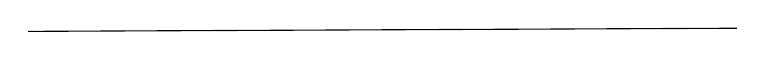
\begin{tikzpicture}\draw (0,0)--(9,0.04);\end{tikzpicture}}

\figure{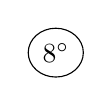
\begin{tikzpicture}[baseline=(n.base)]
\node (n) at (0,0) {$8^{\circ}$};
\draw (0,0) ellipse (0.35 and 0.31);
\end{tikzpicture}}
Si $U$ est un élément de $\mathcal{M}_{\rho,\sigma}$, on lui
associe ses images par $\Theta=\Theta_G$, $\Theta_\rho$, $\Theta_\sigma$, et par
\deleted{$\unsure{\varepsilon_3,\varepsilon_2}$}
$\chi$, $\varepsilon_3$, $\varepsilon_2$, on les note respectivement
\[
\tag{152}
\left\{\begin{array}{l}
\uline{U}\in\Gamma G\\[4pt]
\uline{a}\ \unsure{\in}\Gamma T_\rho\\[4pt]
\uline{b}\in\Gamma N'_\sigma\\[4pt]
\figure{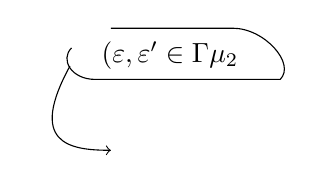
\begin{tikzpicture}[baseline=(e.base)]
\node[inner sep=3pt] (e) at (0,0) {$(\varepsilon,\varepsilon'\in\Gamma\mu_2$};
\draw (-1.25,0.1) .. controls (-1.4,-0.05) and (-1.25,-0.3) .. (-0.95,-0.3)
 -- (1.4,-0.3) .. controls (1.6,-0.1) and (1.2,0.35) .. (0.8,0.35) -- (-0.75,0.35);
\draw[->] (-1.27,-0.13) .. controls (-1.8,-1.1) and (-1.3,-1.2) .. (-0.75,-1.2);
\end{tikzpicture}}\\[4pt]
\mu\in\Gamma G_m
\end{array}\right.
\]

\margin{\unsure{satisfaisant}
\[
\tag{152'}
\left\{\begin{aligned}
\mu&=\delta_G(\uline{U})=\unsure{\delta'_\sigma|\delta_\sigma}(\uline{b})=\varepsilon'\delta_\rho(a)\\
\unsure{\varepsilon'|\varepsilon}&=\varepsilon_\sigma(\uline{b})
\end{aligned}\right.
\]
donc ces quantités sont déterminées par la seule
\unsure{conn.} de $\uline{U},\uline{a},\uline{b}$}

\margin{\figure{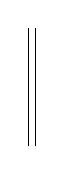
\begin{tikzpicture}
\draw (0,0)--(0,1.5);\draw (0.09,0)--(0.09,1.5);
\end{tikzpicture}}
Il faudrait expliciter que les \unsure{égalités|relations} (152)' \uline{caractérisent}
$\mathcal{M}_{\rho,\sigma}$ comme sous-groupe de $G\times T_\rho\times N'_\sigma$
-- il faudrait faire la vérification, pour se rendre
compte \unsure{si on n'a pas} \unsure{oublié}, dans
\unsure{(135)} des \unsure{hyp$^{\mathrm{ses}}$} à faire\ldots}

\margin{\uline{NB} $G^{\pm1}\overset{\mathrm{d\acute ef}}{=}\operatorname{Ker}\delta_G^2$}

avec des notations du \S\ 46 et suivants.
\unsure{manquent} cependant, \unsure{dans|pour} l'optique \unsure{des} \unsure{points entiers},
les éléments notés précédemment
\diagram{\begin{tikzcd}[ampersand replacement=\&,column sep=small,row sep=small]
\uline{u} \& \alpha \& \beta \& \alpha_0 \& \beta_0 \& f\arrow[lllll,bend right=28]
\end{tikzcd}}
, avec
\[
\left|\begin{aligned}
u&\in\Gamma\unsure{T_0}\subset\Gamma G\\
\alpha,\alpha_0&\in\Gamma G^{\pm1}\subset\Gamma G\\
\beta,\beta_0,f&\in\Gamma SG.
\end{aligned}\right.
\]
reliés \inserted{entre eux et aux précédents,} par des relations
\[
\left\{\diagram{\begin{tikzcd}[ampersand replacement=\&,row sep=small,column sep=normal]
\alpha=\uline{u}\,\uline{a}^{-1}
\& {}\arrow[d,dash,start anchor=north,end anchor=south]
\& |[yshift=-0.8em]|{\text{i.e.}\quad\uline{u}=\alpha\unsure{\overline{a}}=\beta b.}\\
\beta=\uline{u}\,\uline{b}^{-1} \& {} \& \\
\uline{U}=f^{-1}\uline{u}
\arrow[uu,bend left=80,start anchor=west,end anchor=west]
\arrow[u,bend left=70,start anchor=west,end anchor=west] \& \& \\
\alpha_0=f^{-1}\alpha \& \& \text{i.e.}\quad\alpha=f\alpha_0\\
\beta_0=f^{-1}\beta \& \& \text{i.e.}\quad\beta=f\beta_0
\end{tikzcd}}\right.
\]
\margin{formules \uline{dans $G$}}

\margin{\uline{NB} de ces \unsure{6 quantités} (153),
$\uline{u}$ est distingué par le fait d'être
\uline{\unsure{multiplicatif}}
(comme les quantités (152))}

\margin{On pourrait introduire
\[
\left\{\begin{aligned}
\xi&=\alpha\rho(\alpha)^{-1}\\
\eta&=\unsure{\varepsilon}\,\beta\sigma(\beta)^{-1}
\end{aligned}\right.
\quad\unsure{(153)}
\]
\[
\begin{aligned}
g&=\alpha_0\rho(\alpha_0)^{-1}\\
h&=\unsure{\varepsilon}\,\beta_0\unsure{\sigma}(\beta_0)^{-1}
\end{aligned}
\]
mais \unsure{peu} nous \unsure{chaut} ici.}

\mspage{452}

\begin{center}
{\small
452\\
\texttt{https://grothendieck.umontpellier.fr}\\
Université de Montpellier, UMR CNRS 5149, Case courrier 051, Place Eugène Bataillon\\
34095 Montpellier cedex 5 - France
}
\end{center}
% ===== LM_C3-454-472: second pass, checked against the scans =====
\scanpage{454}

formules qui ont un sens seulement si on suppose donnés des plongements (ou du moins morphismes)

\diagram{
\[
(155)\quad
\left\{
\begin{tikzcd}[ampersand replacement=\&,column sep=large]
T_\rho \arrow[r,hook] \& G \\
T_\sigma \arrow[r,hook] \& G
\end{tikzcd}
\right.
\qquad
\begin{gathered}
\text{et un sous-groupe}\\
\begin{tikzcd}[ampersand replacement=\&,column sep=large]
T_0 \arrow[r,hook] \& G
\end{tikzcd}
\end{gathered}.
\]
}

Quand on a de tels plongements, les formules (154) ont un sens, et définissent \deleted{\unsure{toutes les}} (pour les quantités (152) connues) les quantités (153) en termes de l'une \deleted{\unsure{d'elles}}\inserted{d'elles}, disons $\underline u$, ou \deleted{\illegible{1}} $f$, ou $\alpha$, ou $\beta$ (mais pas en termes de $\alpha_0$ ou de $\beta_0$).

En fait, on dispose d'un sous groupe

\diagram{
\[
\begin{array}{r@{\;}c@{\;}l}
\begin{gathered}(156)\\[2em]\deleted{\text{\unsure{tel}}}\\[3em]{}\end{gathered}
&\begin{tikzcd}[ampersand replacement=\&,row sep=3em]
{}\arrow[dd]\\{}\\{}
\end{tikzcd}
&\begin{gathered}
T_0\subset G\\
\text{tel que}\quad
\left\{\begin{array}{l}
\begin{tikzcd}[ampersand replacement=\&,column sep=large]
T_0 \arrow[r,"{\substack{\delta_G|T_0\\\sim}}"] \& G_m
\end{tikzcd}\\[5pt]
\text{i.e.}\quad G\simeq T_0.SG\\
\hspace{6em}\text{produit }1/2\text{ direct},
\end{array}\right.
\end{gathered}
\end{array}
\]
}

de sorte que \deleted{la quantité}\inserted{pour $U\in\Gamma G$,} existe un \uline{unique} \deleted{$f\in\Gamma SG$ tel que}\inserted{couple $(f,u)\in\Gamma(SG\times T_0)$ avec}
\[
U=f^{-1}\underline u.
\]
d'où des uniques $\alpha,\beta,\alpha_0,\beta_0\in\Gamma G$ satisfaisant (avec $f,u$ précédents) à (154) :
\[
(157)\quad
\alpha=\underline u\,\underline a^{-1},\quad
\beta=\underline u\,\underline b^{-1},\quad
\alpha_0=f^{-1}\alpha=f^{-1}\underline u\,\underline a^{-1},\quad
\beta_0=f^{-1}\deleted{\unsure{\alpha}}\inserted{\beta}=f^{-1}\underline u\,\underline b^{-1}.
\]
\mspage{453}
\scanpage{455}
\mspage{530}

On aura d'ailleurs
\[
\deleted{\unsure{\det\underline U=}}\det\underline u
=\det\underline U=\mu
\]
\[
\begin{aligned}
\det\alpha&=\underline{\det}(\underline u)\det(\underline a)^{-1}=\varepsilon'
&&\text{par (152')}\\
\det\beta&=\det(\underline u)\det(\underline b)^{-1}=1\\[3pt]
\text{et}\quad\det\alpha_0&=\det\alpha=\varepsilon'\\
\det\beta_0&=\det\beta=1
\end{aligned}
\]
on aura donc bien
\[
\begin{aligned}
\alpha,\alpha_0&\in\Gamma G^{\pm1}\overset{\text{déf}}=
\{g\mid(\det g)^2=1\}\\
\beta,\beta_0&\in\Gamma SG
\end{aligned}
\]
--- mais on a admis, bien sûr, que les \unsure{hom.} $\delta_\rho,\delta_\sigma$ de (135) sont \unsure{induits}, via les plongements (155), par le déterminant $\delta_G$.

Pour parvenir à la relation \unsure{ou} \unsure{d'équation}
\[
(157)\qquad
\underbrace{[\alpha,\rho]}_{\xi}
=\varepsilon\underbrace{[\beta,\sigma]}_{\eta}\varepsilon_1(\mu-1),
\]
il faut se donner des sections $\rho,\sigma$ de $G$ (\deleted{\unsure{ou}} plus précisément sans doute, \inserted{resp.\textsuperscript{t}} de $T_\rho$ et de $T_\sigma$ maximaux), et un unipotent strict $\varepsilon_1\in\Gamma SG$, pour que la relation (157) prenne un sens.
Remplaçons $\alpha,\beta$ par \unsure{des|les} valeurs $\underline u\,\underline a^{-1},\underline u\,\underline b^{-1}$, la relation devient (utilisant la commutativité de $T_\rho$, \deleted{\unsure{et}} qu'on n'avait pas vraiment fait \unsure{intervenir} jusqu'ici)
\[
(*)\qquad
[u,\rho]
=\varepsilon\cdot\underline u
\bigl(\underline b^{-1}\sigma(\underline b)^{\deleted{\unsure{-1}}}\bigr)^{\deleted{\unsure{-1}}}
\sigma(\underline u)^{-1}\varepsilon_1(\mu-1).
\]
\mspage{454}
\scanpage{456}

et résultera de l'ensemble des deux conditions
\[
(158)\quad
\left\{
\begin{aligned}
\text{a)}\quad&b^{-1}\sigma(b)=\varepsilon_\sigma(b)
&&\text{\uline{identiquement} si }b\in\Gamma N'_\sigma\\
&\text{i.e.}\quad b(\sigma)=\varepsilon_\sigma(b).\sigma
&&\text{identiquement}\\[4pt]
\text{b)}\quad&[u,\rho]=[u,\sigma]\varepsilon_1(\mu-1)
&&\text{identiquement en }u\in\Gamma T_0\\
&&&\text{pour }\mu=\delta_{T_0}(u)\overset{\mathrm{dfn}}=\det(u)\\
&\text{i.e.}\quad\rho(u)=\varepsilon_1(1-\mu)\sigma(u)
&&\text{identiquement en }u
\end{aligned}
\right.
\]
ce qui s'écrit aussi (en appliquant $\sigma^{-1}$ aux deux \unsure{mbs|mb})
\[
\sigma^{-1}\rho(u)=\varepsilon_0(1-\mu).u
\qquad\text{où}\quad\varepsilon_0=\sigma^{-1}(\varepsilon_1)
\]
et n'est guère concevable que si \uline{$T_0$ normalise $L_0$}, et si $\sigma^{-1}\rho\in\Gamma T_0.L_0$ \deleted{et} est de la forme
\[
(159)\quad
\left\{
\begin{aligned}
\text{a)}\quad&\widetilde{\sigma^{-1}\rho}=\widetilde{\varepsilon_0u_0}
\qquad u_0\in\Gamma T_0\\
\text{b)}\quad& T_0\text{ opère sur }L_0\text{ par la \unsure{coaction|action} \unsure{induite}}\\
&\hspace{8em}\text{par le déterminant}
\end{aligned}
\right.
\]
(Il y a quand $\unsure{\overline{\mathrm m}}$ encore de la marge, \unsure{parr|par} aux conditions draconiennes envisagées dans \uline{$\overline{\mathrm{VII}}$} !)

Mais ici l'équation (157) venait un peu comme cheveux sur soupe --- il doit y avoir des façons plus convaincantes et exigeantes de l'amener savoir \deleted{par} en relation avec des formules
\[
(160)\quad
\left\{
\begin{aligned}
\underline U(\rho)&=\operatorname{int}(\alpha_0).\rho
&&\bigl(=\alpha_0\rho(\alpha_0)^{-1}\rho\bigr)\\
\underline U(\deleted{\unsure{\rho}}\inserted{\sigma})&=
\varepsilon\operatorname{int}(\beta_0)\sigma
&&\bigl(=\beta_0\sigma(\beta_0)^{-1}\bigr)\\
\underline U(\varepsilon_0)&=\operatorname{int}(f^{-1})
\bigl(\varepsilon_0^{\deleted{\unsure{\mu}}}\unsure{(\mu)}\bigr)
\end{aligned}
\right.
\qquad
\begin{aligned}
\text{i.e.}\quad[\underline U,\rho]&=\alpha\rho(\alpha)^{-1}\\
[\underline U,\sigma]&=\varepsilon\beta\sigma(\beta)^{-1}
\end{aligned}
\]
\margin{attention au signe $\varepsilon$}

La troisième relation résulte aussitôt de $\underline U=f^{-1}\underline u$, et du fait que par hypothèse \inserted{(159 b)} $\underline u\in\Gamma T_0$ opère sur $L_0$ (\unsure{identiquement}) avec le multiplicateur $\mu=\det(\underline u)$.
\mspage{455}
\scanpage{457}
\mspage{531}

Les deux autres formules s'\unsure{explicitent} successivement, en écrivant $\alpha=\underline u\,\underline a^{-1}$, $\beta=\underline u\,\underline b^{-1}$, $\underline U=f^{-1}\underline u$
\[
\alpha_0=f^{-1}\alpha,\quad\beta_0=f^{-1}\beta
\]
\[
(161)\qquad
\left\{
\begin{aligned}
\underline u(\rho)&=\operatorname{int}(\alpha)(\rho)\\
\underline u(\sigma)&=\varepsilon\operatorname{int}(\beta)(\sigma)
\end{aligned}
\right.
\qquad\text{où }f\text{ ne figure plus}
\]
\[
\begin{aligned}
\text{i.e.}\qquad\underline u(\rho)&=\operatorname{int}(\underline u)(\rho)
&&\text{puisque }\operatorname{int}(\underline a^{-1})\rho=\rho\\
&&&\text{(comme }T_\rho\text{ comm.)}\\
&\text{OK !}\\
\underline u(\sigma)&=\deleted{\illegible{1}}\inserted{\varepsilon}\operatorname{int}(u)
\underbrace{\bigl(\underline b^{-1}(\sigma)\bigr)}_{\substack{=\varepsilon.\sigma\\\text{cf (158)(a)}}}
=\operatorname{int}(u)\sigma\quad\text{OK !}
\end{aligned}
\]

Pour prouver (160) on n'a utilisé que (158 a) et (159) (b). Essayons d'en déduire maintenant la ``relation des lacets'' (157) --- ça doit être un calcul formel, que j'ai déjà dû faire une douzaine de fois, dans des contextes qui se \unsure{différencient} au fur et à mesure ! On élimine $f$ en écrivant les relations (160) sous la forme équivalente (161) et
\[
(161\ \text{bis})\quad
\underline u(\varepsilon_0)=\varepsilon_0(\mu)
\qquad\text{i.e.}\quad
\underbrace{[\underline u,\varepsilon_0]}_{u\varepsilon_0(u)^{-1}}
=\varepsilon_0(\mu-1)\qquad\deleted{\unsure{\operatorname{int}}}
\]
\[
\deleted{\text{i.e.}\quad u\varepsilon_0(u)^{-1}}
\]
\[
\begin{array}{l|ll}
\begin{aligned}[t]
\text{or}\qquad&\\
[\underline u,\varepsilon_0]&=
u\underbrace{\varepsilon_0(u)^{-1}}_{\substack{\unsure{\text{i.e.}}\ \sigma^{-1}\rho(u)^{\deleted{\unsure{-1}}}}}\\
\text{i.e.}\quad\sigma([u,\varepsilon_0])&=\sigma(u)\rho(u)^{-1}
\end{aligned}
&
\begin{aligned}[t]
\text{or}\quad&\deleted{\rho(u)=\rho u\rho^{-1}=}\\
&u\rho u^{-1}\rho^{-1}=\xi\\
&\rho(u^{-1})=u^{-1}\xi\\
&\rho(u)=\xi^{-1}u\\
\unsure{\text{de}=|\text{de }\overline{\mathrm m}}\quad&\sigma(u)=\deleted{\unsure{\varepsilon}}\eta^{-1}u
\end{aligned}
&
\begin{aligned}[t]
\xi&\overset{\mathrm{dfn}}{=}\alpha\rho(\alpha)^{-1}\\[4em]
\eta&\overset{\mathrm{dfn}}{=}\varepsilon\beta\sigma(\beta)^{-1}
\end{aligned}
\end{array}
\]
\[
\text{d'où}\qquad
\sigma([u,\varepsilon_0])=
\deleted{\unsure{\xi^{-1}u\eta^{-1}u}}\eta^{-1}\xi
\]
et \unsure{(*)|($\alpha$)} devient, en appliquant $\unsure{\sigma}$
\[
\eta^{-1}\xi=\varepsilon_1(\mu-1)
\qquad\text{i.e.}\quad\xi=\eta\varepsilon_1(\mu-1)
\qquad\text{i.e. (157)}
\]
\hfill OK !
\mspage{456}
\scanpage{458}

En résumé :

\uline{Proposition} Supposons donnés, en plus des données de la section précédente $7^\circ$ (p. 526' ff \unsure{\}|)}, notamment (135)(136)), \deleted{des sections $\rho$ de $\unsure{T_{\rho,\sigma}|T_\rho,\sigma}$} ceci

\diagram{
\[
(162)\quad\left\{
\begin{array}{ll}
\text{a)}&\text{section }\rho\in\Gamma T_\rho,\quad\sigma\in\Gamma T_\sigma\quad\text{sections \uline{centrales}}\\[4pt]
\text{b)}&\text{Plongements}\quad
\begin{tikzcd}[ampersand replacement=\&,column sep=large]
T_\rho \arrow[r,hook] \& G
\end{tikzcd},\quad
\begin{tikzcd}[ampersand replacement=\&,column sep=large]
N'_\sigma \arrow[r] \& G
\end{tikzcd}\\[4pt]
\text{c)}&\text{tore}\quad
\begin{tikzcd}[ampersand replacement=\&,column sep=large]
T_0 \arrow[r,hook] \& G
\end{tikzcd}\quad\text{tel que }\delta_G:\quad
\begin{tikzcd}[ampersand replacement=\&,column sep=large]
\unsure{T_0} \arrow[r,"\sim"] \& G_m
\end{tikzcd}\\
&\text{i.e.}\quad G\simeq T_0.SG\quad\text{(semi-direct)}\\[4pt]
\text{d)}&\varepsilon_0\in\Gamma G\quad\text{unipotent \deleted{strict} régulier, définissant}\\
&\text{donc}\quad
\begin{tikzcd}[ampersand replacement=\&,column sep=large]
\unsure{\lambda} \arrow[r,mapsto] \& \varepsilon_0(\lambda)
\end{tikzcd}:\quad
\begin{tikzcd}[ampersand replacement=\&,column sep=large]
G_a \arrow[r,hook] \& SG
\end{tikzcd}
\end{array}\right.
\]
}

et supposons \deleted{(en plus de la \uline{commutativité} de $T_\rho,T_\sigma$}
\[
\begin{aligned}
\inserted{\text{a)}\quad\delta_G|T_\rho=\delta_\rho,\quad\delta_G|N'_\sigma=\delta_\sigma}\\
\deleted{\text{a)}\quad T_0\text{ \unsure{normalise} }\unsure{L_0}}
\end{aligned}
\]
\[
(163)\quad
\begin{aligned}
\text{b)}\quad&\operatorname{int}(\underline b)(\sigma)=\varepsilon_\sigma(\underline b)\sigma
\quad\text{dans }G\text{ identiquement}\\
&\hspace{12em}\text{pour }\underline b\in\Gamma\unsure{N'_\sigma|N^2_\sigma}\\[4pt]
\text{c)}\quad&T_0\text{ normalise }L_0,\text{ et on a}\\
&u(\varepsilon_0(\lambda))=
\varepsilon_0\bigl(\deleted{\unsure{\delta_G(u)}}\mu\lambda\bigr)
\quad\text{où }\mu=\delta_G(u)\\[4pt]
\text{d)}\quad&\widetilde{\unsure{\sigma|\rho}}^{-1}\widetilde\rho
\in\deleted{\unsure{\widetilde T_0}}\Gamma\widetilde\varepsilon_0\widetilde L_0
\quad\text{i.e. }\exists\text{loc.}^{\text{t}}\text{ section }\lambda_0\in\Gamma G_m\\
&\text{avec}\quad\lambda_0\widetilde\sigma^{-1}\widetilde\rho=\varepsilon_0u_0,
\quad\text{avec }u_0\in\Gamma T_0
\end{aligned}
\]
\margin{\unsure{relie} $L_0,T_0$}
\margin{$\begin{array}{l|}\text{\unsure{relie}}\quad L_0,T_0\\\rho,\sigma\end{array}$}

Sous ces conditions, on a pour tt système (152) satisfaisant les relations (152') (i.e. en fait pour tte \deleted{\unsure{syst}} section de $\mathcal M_{\rho,\sigma}$ !) un unique \unsure{syst.} (153), satisfaisant les relations (154) --- savoir $\underline U$ se met de façon unique sous la forme
\[
(164)\quad\underline U=f^{-1}\underline u,\qquad f\in\Gamma SG,\quad\underline u\in\Gamma T_0
\]
et on pose
\[
\begin{aligned}
(165)\quad\alpha&=\underline u\,\underline a^{-1},\quad
\beta=\underline u\,\underline b^{-1},\quad
\alpha_0=f^{-1}\unsure{\alpha|\alpha_\rho}=
\deleted{\unsure{\beta}}\inserted{f}^{-1}\underline u\,\underline a^{-1},\\
\beta_0&=f^{-1}\beta=f^{-1}\underline u\,\underline b^{-1}.
\end{aligned}
\]
\mspage{457}
\scanpage{459}
\mspage{532}

Tout ceci posé, on a alors les formules
(160), (161), (161 bis), et la formule ``du lacet'' (157).

Nous nous posons maintenant la question
sous quelles conditions la connaissance de
$(\alpha,\beta,f)$ (p.ex.) parmi les quantités (153),
permet de récupérer les quantités (152) ---
i.e. une section de $\mathcal M_{\rho,\sigma}$ --- et quelles conditions
il faut imposer à $(\alpha,\beta,f)$. Il
suffirait \inserted{(pour l'unicité)} de pouvoir construire $\underline u$, d'où
$\underline U,\underline a,\underline b$ par les trois premières formules
(154). \deleted{\unsure{Si, d'autre part on a}} Il faut
donc trouver $\underline a\in\Gamma T_\rho$ tel que $\alpha\underline a$ soit section
de $T_0$, --- indétermination sur $\underline a$ est de
$\Gamma T_0\cap T_\rho$, et $\underline b\in\Gamma N'_\sigma$ tel que $\beta\underline b$ soit section
de $T_0$ --- indétermination dans \deleted{$\unsure{\Gamma N'_\sigma\cap}$} $\Gamma T_0\cap N'_\sigma$.
L'indétermination sur $\underline u$ est la multiplication
à droite par une section de $T_0\cap T_\rho\cap N'_\sigma$, il
suffira donc qu'on ait
\[
\text{(164)}\qquad T_0\cap T_\rho\cap N'_\sigma=\{1\}.
\]
\margin{en fait, on aura $\unsure{\overline{\mathrm m}}$ $T_0\cap T_\rho=\{1\}$ dans les cas \unsure{envisagés} dans \uline{II}, \uline{III} et \unsure{suivants|suite}\ldots}
Supposant cette relation satisfaite, quelles
conditions mettre sur $(\alpha,\beta,f)$ pour provenir
d'un \unsure{syst.} (152) --- i.e. d'une section de $\mathcal M_{\rho,\sigma}$ ?

\mspage{458}
\scanpage{460}

On voit que \unsure{si} une section \deleted{$\unsure{\varphi}$} $\varphi_0$ de $\mathcal M_{\rho,\sigma}$, \deleted{est}
\deleted{\unsure{rempl.}} correspondant à $\alpha_0,\beta_0,f_0$, est remplacé
par $\varphi_1\overset{\unsure{\text{déf}}}{=}f^{-1}.\varphi_0$, correspondant à $\alpha_1,\beta_1,f_1$, alors
\[
\text{(165)}\qquad \alpha_1=\alpha_0,\quad\beta_1=\beta_0,\quad f_1=f_0f,
\]
car on voit que si $\varphi_0$ correspond à $(\underline U_0,\underline a_0,\underline b_0)$,
alors $\varphi_1$ à $(U_1,\underline a_1,\underline b_1)$, alors on a
\[
\text{(166)}\qquad U_1=f^{-1}U_0,\quad\underline a_1=\underline a_0,\quad\underline b_1=\underline b_0
\]
(car $\Theta_G\mid SG=$ l'inclusion canonique $SG\hookrightarrow G$,
et $\Theta_\rho$\inserted{$,\Theta_\sigma$} \deleted{est} triviaux sur $SG$). \deleted{Donc Cela
montre que} \inserted{Donc \deleted{\unsure{il}}} on aura
\[
u_1=u_0\qquad (\text{car }\det U_1=\det U_0)
\]
d'où (165). Cela montre que les conditions
cherchées sur $(\alpha,\beta,f)$ ne dépendent que de
$\alpha,\beta$, pas de $f$. On voudrait qu'elles
s'expriment par la validité de la formule des
lacets\inserted{(157)}, pour un paramètre \inserted{$\varepsilon,$} $\mu$ non précisés $(\varepsilon^2=1)$
(qui \unsure{sera} alors uniquement déterminé --- et \unsure{permettra}
la \unsure{définition sec.} de \unsure{notion locale|action locale}\ldots).

\margin{à vrai dire, cette condition n'est pas \uline{suffisante} $\overline{\mathrm m}$ dans les cas envisagés --- on trouvera \unsure{donc|dans} un $\underline u\in B'_0$, et il faut exiger que $\underline u\in T_0$ (déjà pour $(\alpha,\beta)$ soit ``normalisé'') i.e. $B=0$, où $B=ac+bd+bc$, si $\underline u=\left(\begin{smallmatrix}a&b\\c&d\end{smallmatrix}\right)$ (cas modulaire) cf prop. p.~412'\ldots\ \unsure{Pour l'avoir} $\unsure{R}$ ; \unsure{lui-même étant} \unsure{condition supplém.}, \unsure{il|qui} \unsure{faut remplacer|faut envisager} $\mathcal M_{\rho,\sigma}$ \unsure{par le produit} $\tfrac12$ \unsure{direct par} $L_0$, \unsure{sur lequel on fait} $\unsure{f_\Delta}=\unsure{0}$, \unsure{soit} $S\mathcal M_{\rho,\sigma}$.}

La suffisance de cette condition \unsure{fera}
l'objet des réflexions des (II) (III),
\unsure{sous} des conditions (plus draconiennes que celles
\unsure{de la} prop. précédente (p.~531') que nous
avons imposées au triplet $(\varepsilon_0,\rho,\sigma)$. Il

\mspage{459}
\scanpage{461}
\mspage{533}

est possible que les conditions auxquelles nous
\inserted{\unsure{y}} sommes parvenus étaient plus restrictives
que nécessaires, et que je sois obligé
d'y revenir par la suite, dans un contexte
plus général que celui des formes de
$\mathrm{Gl}(2)$, $\mathrm{GP}(1)$, $\mathrm{Sl}(2)$, mais pour le moment
l'étude détaillée faite en nous inspirant
des hypothèses dégagées dans \deleted{\unsure{les}} II, III nous
aura servi de déblayage, pour nous éclairer
les idées sur un cas particulier
important.

\uline{Rem.} Rappelons que nous avons vu qu'en
fait $\mu$ est déjà défini en termes de $\alpha$ seul,
et $\overline{\mathrm m}$ en termes de $\alpha\rho(\alpha)^{-1}=\xi$ \unsure{;} \deleted{\unsure{bien|donc}}
Mais il n'est déterminé en termes de $\beta$
--- en fait, de $\beta\sigma(\beta)^{-1}$ --- que modulo
la connaissance de $\varepsilon$ (en pratique, modulo
signe\ldots). Mais si l'on impose (p.ex.) $\varepsilon=1$,
la donnée de $\alpha$ ne détermine $\beta$ que
modulo \deleted{$\unsure{\beta}$} $\beta\longrightarrow\beta T_\sigma$\ldots

\mspage{460}
\scanpage{462}

La structure de $\mathcal M_{\rho,\sigma}$ étant bien comprise,
revenons sur le groupe $S\mathcal M_{\rho,\sigma}$\inserted{(cf p.~495')}, considéré comme
produit semi-direct de $\mathcal M_{\rho,\sigma}$ par le sous-groupe
$L_0$ de $SG$, sur lequel en fait opère $\mathcal M_{\rho,\sigma}$
via $\chi$. Désignant par

\noindent (165)\quad
\diagram{\begin{tikzcd}[ampersand replacement=\&,column sep=large]
\deleted{\unsure{\varepsilon_0}:\unsure{U}}\;\inserted{\unsure{\mathcal E|\varepsilon}_{L_0}:G_a} \arrow[r,"\sim"] \&
\operatorname{Ker}\bigl(S\mathcal M_{\rho,\sigma}\longrightarrow\mathcal M_{\rho,\sigma}\bigr)
\end{tikzcd}}

\inserted{correspondant à $\varepsilon_0$,}
on aura par \deleted{\unsure{définition}} construction
\[
\text{(166)}\qquad
U\bigl(\unsure{\mathcal E|\varepsilon}_{L_0}(\lambda)\bigr)
=\unsure{\mathcal E|\varepsilon}_{L_0}(\mu\lambda)
\qquad\text{où }\mu=\chi(U).
\]

\deleted{Le groupe $S$}

\mspage{461}
\scanpage{463}
\mspage{534}

\deleted{\unsure{XI}} \textcircled{$9^\circ$} \uline{Les sous-groupes}
$\mathcal M_{\rho,\sigma}(0)$,
\deleted{$\mathcal M_{\rho,\sigma}(\tfrac12),\mathcal M_{\rho,\sigma}(-\unsure{\overline J|\overline\jmath})$.}
\inserted{$\mathcal M_{\rho,\sigma}[0]$, et le groupe}
$S\mathcal M_{\rho,\sigma}$, l'isom.
\diagram{\begin{tikzcd}[ampersand replacement=\&,column sep=large]
S\mathcal M_{\rho,\sigma} \arrow[r,"\sim"] \& \Sigma^+_{\rho,\sigma}
\end{tikzcd}}

Le groupe $\mathcal M_{\rho,\sigma}$ est extension de $\mathcal T_{\rho,\sigma}$ par
$\unsure{\widetilde G|\widetilde{\mathcal C}}^+_{\rho,\sigma}\simeq SG$, et les trois sous-groupes que nous allons
expliciter seront des \deleted{sections}\inserted{\unsure{ss-groupes|sous-groupes}}, \deleted{partielle} avec le
grain de sel que pour le troisième, ce sera une
section partielle seulement, au dessus du
sous-groupe \inserted{$\mathcal T'_{\rho,\sigma}$} d'indice $2$ de $\mathcal T_{\rho,\sigma}$, noyau de
$\varepsilon_3$.

$[\![$Déterminons de façon générale les sections
de $\mathcal M_{\rho,\sigma}$ sur $\mathcal T_{\rho,\sigma}$. Comme on a

\noindent (1)\quad
\diagram{\begin{tikzcd}[ampersand replacement=\&,column sep=large,row sep=small]
R_{\rho,\sigma} \arrow[r] \arrow[d,phantom,"{\unsure{\wr|\simeq}}" description] \& \mathcal T_{\rho,\sigma} \quad \text{épi de noyau }\mu_2\\
S'T_\rho\times SN'_\sigma\times G_m \&
\end{tikzcd}}

\margin{finalement ça servira pas à grand chose\ldots}

il revient au $\overline{\mathrm m}$ de se donner une section,
ou : un hom.

\noindent (2)\quad
\diagram{\begin{tikzcd}[ampersand replacement=\&,column sep=large]
R_{\rho,\sigma} \arrow[r,"{\deleted{\unsure{\Xi|\zeta}}\inserted{\psi}}"] \& \mathcal M_{\rho,\sigma}
\end{tikzcd}}

qui soit \deleted{trivial}
\[
\text{(3)}\qquad
\left\{\begin{aligned}
\text{a)}\quad &\text{trivial sur }\mu_2\\
\text{b)}\quad &\deleted{\unsure{\Xi|\Sigma}(x)\unsure{\equiv|=}x\ \bigl(\unsure{\widetilde G|\widetilde{\mathcal C}}^+_{\rho,\sigma}\bigr)\quad\text{identiquement}.}\quad\inserted{\text{``remonte'' (1)}}
\end{aligned}\right.
\]

Les hom. $\unsure{\Xi|\Sigma}$ qui satisfont à (3) correspondent
aux scindages de l'extension \uline{triviale} de
$R_{\rho,\sigma}$ par $SG$ (extension \uline{produit}), donc
simplement aux \uline{homomorphismes}

\noindent (4)\quad
\diagram{\begin{tikzcd}[ampersand replacement=\&,column sep=large]
R_{\rho,\sigma} \arrow[r,"{\deleted{\unsure{\Xi|\zeta}_{\unsure{0}}}\inserted{\psi^0}}"] \& SG
\end{tikzcd}},

\mspage{462}
\scanpage{464}

en associant à $\psi^0\deleted{\unsure{\xi_0}}$ le hom.
\[
(5)\qquad x\longmapsto \deleted{\unsure{\xi}}\psi(x)
=x\deleted{\unsure{\xi}}\psi^0(x)
=\deleted{\unsure{\xi(x)x}}\psi^0(x).x
\]
Donc la condition a prend la forme
\[
(6)\qquad \deleted{\unsure{\xi}}\psi^0_{\unsure{0}}(x)=x
\quad\text{sur }\mu_2=R_{\rho,\sigma}\cap SG.
\]

\margin{\deleted{\unsure{$\rho$}}}
Les $\psi,\psi^0$ correspondants aux \deleted{\unsure{« trois »}} sections
$\mathcal M_{\rho,\sigma}^{(0)}$, $\mathcal M_{\rho,\sigma}^{(\frac12)}$,
$\mathcal M_{\rho,\sigma}^{(-\overline J)}$ seront notés resp.\textsuperscript{t}
\[
(\psi_{\unsure{0}},\psi^0_0),\ (\psi_{1/2},\psi^0_{1/2}),\
(\psi_{-\overline J},\psi^0_{-\overline J}).\qquad\big]\!\big]
\]

1°) \uline{Cas de} $\mathcal M_{\rho,\sigma}^{(0)}$. Avec les notations
de la p. 529, il \unsure{correspondra} \deleted{\unsure{$\underline U$ et les}}
\inserted{\unsure{$\underline u$}} de $\mathcal M_{\rho,\sigma}$ satisfaisant à l'une des conditions
\uline{équivalentes}
\[
(7)\qquad f=1,\quad\inserted{\underline U=\underline u,}\quad
\underline U\in\Gamma T_0,\quad \alpha_0=\alpha,\quad\beta_0=\beta
\]
donc on a
\[
(8)\qquad \mathcal M_{\rho,\sigma}^{(0)}=\Theta^{-1}(T_0).
\]
\inserted{(en termes de la description de $\mathcal M_{\rho,\sigma}$ de p. 526' ff)}

Vérifions que c'est un \unsure{sous-groupe-section}.
On a
\[
\overbrace{\mathcal M_{\rho,\sigma}^{(0)}\cap\widetilde{\unsure{G|\mathcal C}}_{\rho,\sigma}^{+}}
^{\inserted{(\Theta|SG)^{-1}(T_0)}}=\{1\}
\]
\margin{\unsure{et}}
car $\Theta|(\widetilde{\unsure{G|\mathcal C}}_{\rho,\sigma}^{+}=SG)$ est l'inclusion
canonique $SG\hookrightarrow G$, or $SG\cap T_0=\{1\}$.
Reste à vérifier que
\diagram{\begin{tikzcd}[ampersand replacement=\&]
\mathcal M_{\rho,\sigma}^{(0)} \arrow[r] \& \mathcal T_{\rho,\sigma}
\end{tikzcd}}
(qui est mono par \unsure{$(a)$|$(\alpha)$}) est épi. Mais en

\mspage{463}
\scanpage{465}
\mspage{535}

termes de la \unsure{réalisation} can.
\[
(9)\qquad\mathcal M_{\rho,\sigma}\simeq
\underbrace{R_{\rho,\sigma}\times SG}_{\widetilde{\mathcal M}_{\rho,\sigma}}
/\underset{\text{diagonal}}{\mu_2}
\]
et de l'hom
\margin{\diagram{\begin{tikzcd}[ampersand replacement=\&]
\kappa:R_{\rho,\sigma}\arrow[r]\&\mathbf G_m
\end{tikzcd}}
l'hom canonique \unsure{permettant} d'exprimer $\Theta|R_{\rho,\sigma}$}
\diagram{\begin{tikzcd}[ampersand replacement=\&]
(10)\qquad i_{T_0}:\mathbf G_m\arrow[r,"\sim"]\&T_0\arrow[r,hook]\&G
\end{tikzcd}}
\unsure{isom|hom} inverse de l'isom
\diagram{\begin{tikzcd}[ampersand replacement=\&]
\delta_{T_0}=\det|T_0:\quad T_0\arrow[r,"\sim"]\&\mathbf G_m,
\end{tikzcd}}
on a, pour un élément
\diagram{\begin{tikzcd}[ampersand replacement=\&,column sep=1em,row sep=.2em]
(\underline r,\&U_0)\\
\inserted{R_{\rho,\sigma}}\arrow[u]\&\inserted{SG}\arrow[u]
\end{tikzcd}}
de $\Gamma\widetilde{\mathcal M}_{\rho,\sigma}$
\[
\Theta(\underline r,U_0)=\kappa(\underline r)U_0,\quad
\text{déterminant }\kappa(r)^2
\]
dire que c'est $\unsure{\in U}$ signifie donc l'on a
\[
\kappa(\underline r)U_0=i_{T_0}(\kappa(\underline r)^2)
\quad\text{i.e. }\deleted{\unsure{U_0=}}
\]
\[
(11)\qquad U_0=\kappa(\underline r)^{-1}i_{T_0}(\kappa(\underline r)^2)
\]
donc l'image inverse $\widetilde{\mathcal M}_{\rho,\sigma}^{(0)}$ de
$\mathcal M_{\rho,\sigma}^{(0)}$ dans $\widetilde{\mathcal M}_{\rho,\sigma}$ est formée des
\[
(12)\qquad
\bigl(\underline r,\kappa(\underline r)^{-1}i_{T_0}(\kappa(\underline r))^2\bigr)
\in\Gamma\widetilde{\mathcal M}_{\rho,\sigma}
\]
en d'autres termes cela correspond à un \unsure{groupe} section, avec
\[
(13)\qquad\psi^0_0(\underline r)=\kappa(\underline r)^{-1}i_{T_0}(\kappa(\underline r)^2).
\]
Comme il se doit, on a bien là un \uline{hom}
\diagram{\begin{tikzcd}[ampersand replacement=\&]
\psi^0_0:R_{\rho,\sigma}\arrow[r]\&SG
\end{tikzcd}}
et sa valeur sur $\mu_2$ est l'identité,
car $\kappa(\underline r)^2=1$ et on a
\[
\psi^0_0(r)=\kappa(\underline r)^{-1}=
\begin{gathered}\kappa(\underline r)\\\Vert\\\underline r\end{gathered}
\]

\uline{Remq}\quad\deleted{Avant de \unsure{qui}}
Pour définir cette section, il suffisait

\mspage{464}
\scanpage{466}

(au pt de vue du pur calcul) de se donner un hom quelconque, noté
$\unsure{i'_{T_0}|i_{T_0}}$, de $\mathbf G_m$ dans $SG$, et de poser (13).

Avant de quitter $\mathcal M_{\rho,\sigma}^{(0)}$, je vais introduire le groupe
un peu plus grand (de dim 4, au lieu de 3)
\[
(14)\qquad\mathcal M_{\rho,\sigma}^{[0]}
\overset{\mathrm{dfn}}{=}\Theta^{-1}(B'_0)
\]
où, on le rappelle, $B'_0$ est défini comme le produit $\frac12$ direct
\[
(15)\qquad B'_0=T_0.L_0
\]
Cette fois-ci, $U=U_0\kappa(r)\inserted{\in\Gamma B'_0}$ n'est pas déterminé
par la seule connaissance de son déterminant\inserted{\unsure{$2$}}
$\underline\kappa(r)^2$, qui ne le détermine que modulo $L_0$.
Cela correspond au fait que
$\underset{\inserted{=B'_0\cap SG}}{
\mathcal M_{\rho,\sigma}^{[0]}\cap
\overbrace{\widetilde{\unsure{G|\mathcal C}}_{\rho,\sigma}^{+}}^{\inserted{SG}}}$
n'est plus réduit à $(1)$, mais à $L_0$, qui apparaît donc comme
un sous-groupe invariant de $\mathcal M_{\rho,\sigma}^{[0]}$, et on \unsure{aura|a} évidemment
(compte tenu que $\mathcal M_{\rho,\sigma}^{(0)}\subset\mathcal M_{\rho,\sigma}^{[0]}$ et
\diagram{\begin{tikzcd}[ampersand replacement=\&]
\mathcal M_{\rho,\sigma}^{(0)}\arrow[r,"\sim"]\&\mathcal T_{\rho,\sigma}
\end{tikzcd}}) \unsure{par|que}
\[
(16)\qquad\begin{aligned}
\mathcal M_{\rho,\sigma}^{[0]}&=\mathcal M_{\rho,\sigma}^{(0)}.L_0\\
&\qquad\text{produit }\frac12\text{ direct}
\end{aligned}
\]
C'est encore une construction qui a un sens dès que l'on a un $T_0$ comme dessus,
\deleted{\illegible{2}} et un sous-groupe \deleted{\uline{\unsure{affine}}} $L_0$ de $SG$,

\mspage{465}
\scanpage{467}
\mspage{536}

\unsure{invarié} par $T_0$. \deleted{\unsure{On}}

L'opération de $\mathcal M_{\rho,\sigma}^{[0]}$ sur $SG$ se fait
par l'intermédiaire de $\Theta$, depuis peu regardé comme un épi
\diagram{\begin{tikzcd}[ampersand replacement=\&]
\mathcal M_{\rho,\sigma}^{[0]}
\arrow[r,"\Theta|\mathcal M_{\rho,\sigma}^{[0]}"]\&B'_0
\end{tikzcd}};
cette opération étant précisée, on peut introduire
\margin{pour une définition plus \unsure{transparente}, cf p. 538', 539}
\[
(17)\qquad\deleted{\unsure{\mathcal S}}
S\mathcal M_{\rho,\sigma}\overset{\text{déf}}{=}
\begin{gathered}
\mathcal M_{\rho,\sigma}^{[0]}.SG\\
\text{produit }\frac12\text{ direct}
\end{gathered}
\]
en lequel $SG$ est invariant, et $\mathcal M_{\rho,\sigma}^{[0]}$ s'identifie
à un sous-groupe de $S\mathcal M_{\rho,\sigma}$. Comme
$\mathcal M_{\rho,\sigma}^{(0)}\subset\mathcal M_{\rho,\sigma}^{[0]}$,
on a une inclusion can.
\[
(18)\qquad
\underbrace{\mathcal M_{\rho,\sigma}^{(0)}:SG}_{\unsure{\simeq\mathcal M_{\rho,\sigma}}}
\subset
\underbrace{\mathcal M_{\rho,\sigma}^{[0]}.SG}_{=S\mathcal M_{\rho,\sigma}}
\]
dont l'image est \deleted{\unsure{notée} $S\mathcal M_{\rho,\sigma}^{(0)}$}
identifiée à $\mathcal M_{\rho,\sigma}$.
\deleted{Ceci dit, le sous-groupe $L_0$ de $\mathcal M_{\rho,\sigma}^{[0]}$
cf (16) \unsure{opère} trivial\textsuperscript{t} sur $SG$,
i.e. $\Theta\inserted{|\mathcal M_{\rho,\sigma}^{[0]}}$,
qui est trivial en effet sur $L_0$}

\deleted{\unsure{Revenons|Reprenons}} je commence à \unsure{nouveau} à m'y perdre, je vais me raccrocher
--- pour une compréhension de la signification "géom." de
$S\mathcal M_{\rho,\sigma}$, $\mathcal M_{\rho,\sigma}^{[0]}$, aux notations
de la p. 529, qui mérite d'être \unsure{explicité|explicitée} par un

\mspage{466}
\scanpage{468}

\uline{Proposition}\quad Considérons l'hom
\diagram{\begin{tikzcd}[ampersand replacement=\&,column sep=large,row sep=large]
(19)\quad\mathcal M_{\rho,\sigma}\arrow[r]
\&G\times T_\rho\times N'_\sigma\times\mathbf G_m\times
\unsure{\mu_2^2|\mu_2}
\deleted{\unsure{(\mathbf G_m^3\times\mathbf G_m\times\mu_2)}}\\
x\arrow[r,mapsto]
\&(\Theta_G(x),\Theta_\rho(x),\Theta_\sigma(x),\chi(x),\varepsilon_2(x),\varepsilon_3(x))
\end{tikzcd}}
C'est un monomorphisme, dont l'image est
formée des \deleted{triplets}\inserted{\unsure{syst.}}
$(\underline U,\underline a,\underline b,\inserted{\mu,\varepsilon,\varepsilon'})$
satisfaisant à
\[
\deleted{\unsure{\mu=|\text{pour}}\,
\unsure{\det_G|\delta_G}(\underline U)
=\delta_\rho(\underline b)=\varepsilon\det}
\]
\[
(20)\qquad\left\{\begin{aligned}
\mu&=\delta_G(\underline U)=\delta_\sigma(\underline b)
=\varepsilon'\delta_\rho(\underline a)\\
\varepsilon&=\varepsilon_\sigma(\underline b)\\[1ex]
\end{aligned}\right.
\]

\uline{Corollaire}. Le morphisme.
\diagram{\begin{tikzcd}[ampersand replacement=\&,column sep=large,row sep=large]
{}\arrow[d,no head,"(21)"']\&\mathcal M_{\rho,\sigma}\arrow[r]
\&G\times T_\rho\times N'_\sigma\\
{}\&x\arrow[r,mapsto]\&\Theta_G(x),\Theta_\rho(x),\Theta_\sigma(x)
\end{tikzcd}}
est un monomorphisme, l'image est formée des triplets
$(\underline U,\underline a,\underline b)$ satisfaisant à
\margin{\uline{NB} on a
$\left\{\begin{aligned}
\varepsilon&=\varepsilon_\sigma(\underline b)\\
\varepsilon'&=\delta_\rho(\underline a)/\delta_\sigma(\underline b)\\
\mu&=\delta_\sigma(\underline b)=\delta_G(\underline U)
\end{aligned}\right.$}
\[
(22)\qquad\left\{\begin{aligned}
\delta_G(\underline U)&=\delta_\sigma(\underline b),\\
[\delta_\rho(\underline a)/\delta_\sigma(\underline b)]^2&=1.
\end{aligned}\right.
\]

\uline{Dém. de la proposition.}\quad On a
\deleted{$\unsure{\operatorname{Ker}(\Theta_G)|\mu_G}$}
\[
\operatorname{Ker}(\Theta_G,\deleted{\unsure{\chi|\xi_2}},\varepsilon_2,\varepsilon_3)
=SR_{\rho,\sigma}^{\unsure{\circ|0}}\simeq ST_\rho\times ST_\sigma
\]
et $\Theta_\rho,\Theta_\sigma$ \deleted{\unsure{donc|des}}
sur $SR_{\rho,\sigma}^{\unsure{\circ|0}}$ s'identifient aux deux projections,
donc \deleted{$\unsure{\Theta}$}
\[
\operatorname{Ker}\bigl((\Theta_\rho,\Theta_\sigma)|SR_{\rho,\sigma}^{\unsure{\circ|0}}\bigr)
=\{1\},\quad\text{donc}
\]
\[
\operatorname{Ker}(\Theta_G,\chi,\varepsilon_2,\varepsilon_3,\Theta_\rho,\Theta_\sigma)
=(1),
\]

\mspage{467}
\scanpage{469}
\mspage{537}

donc mono. Pour l'épi, on est ramené à la forme équivalente du Corollaire. --- OPS qu'on a un $\lambda$ tel que
\[
\lambda^2=\mu\overset{\mathrm{dfn}}{=}\det\underline U
\]
on veut écrire
\[
\underline U=\Theta_{\widetilde{\mathcal M}}
\left(\underset{\underset{R_{\rho\sigma}}{\rotatebox{90}{$\in$}}}{r},
\underset{\underset{SG}{\rotatebox{90}{$\in$}}}{U_0}\right)
=\kappa(r)U_0
\]
\margin{NB $\Theta_{\widetilde{\mathcal M}}$ l'hom can.
\diagram{\begin{tikzcd}[ampersand replacement=\&]
\widetilde{\mathcal M}_{\rho,\sigma}\overset{\mathrm{dfn}}{=}R_{\rho,\sigma}\times SG \arrow[r] \& G
\end{tikzcd}}
que j'\unsure{avais|écrivais|écris} $\Theta_G$.}
avec $U_0\in\Gamma(SG)$, i.e. $\kappa(r)^2=\det\underline U$ i.e. $\kappa(r)^2=\mu$,
on prendra $r$ avec \deleted{$\unsure{\kappa}$}
\[
\kappa(r)=\lambda,
\]
\deleted{\unsure{alors}} on pose donc
\[
\underline U_0=\lambda^{-1}U,\quad
\underline a_0=\lambda^{-1}\underline a,\quad
\underline b_0=\lambda^{-1}b
\]
\deleted{\unsure{et on est}} \inserted{et on est} ramené à voir que $\underline U_0,\underline a_0,\underline b_0$ sont dans l'image de $\mathcal M_{\rho,\sigma}$ (en \unsure{étant|ôtant} des ``\unsure{corrigés}'' $(\underline U,\underline a,\underline b)$ par l'image \deleted{\unsure{dans le}} $G\times T_\rho\times\unsure{T_\sigma}$ de la section $\lambda$ de $G_m\hookrightarrow R_{\rho,\sigma}$). On est ramené à voir que $(\underline a_0,\underline b_0)$ est dans l'image de
\diagram{\begin{tikzcd}[ampersand replacement=\&]
R_{\rho,\sigma}\arrow[r] \& \deleted{\unsure{T}}T_\rho\times N'_\sigma.
\end{tikzcd}}
Mais maintenant $\underline a_0$ est dans $S'T_\rho$, $\underline b_0$ dans $SN'_\sigma$, et justement $R_{\rho,\sigma}\simeq S'T_\rho\times SN'_\sigma$, \unsure{c'est gagné}\ldots

\uline{Remarque}. On ne peut remplacer $G$ par $PG$,
i.e.
\diagram{\begin{tikzcd}[ampersand replacement=\&]
\mathcal M_{\rho,\sigma}\arrow[r] \& PG\times T_\rho\times N'_\sigma
\end{tikzcd}}
(où on peut rajouter encore $G_m\times\mu_2\times\mu_2$ si on veut!) n'est \uline{pas} mono --- son noyau est justement le sous-groupe $\mu_2$ de $\widetilde{\unsure{G|\mathcal C}}_{\rho,\sigma}^{+}=SG$.

\mspage{468}
\scanpage{470}

Considérons, maintenant que les quantités $\underline U,\underline a,\underline b$ $(\inserted{et}\ \mu,\varepsilon,\varepsilon')$ de p.~529 (152) sont comprises, les quantités (153) du loc. cit $\underline u,f,\alpha,\beta,\alpha_0,\beta_0$ ($g,h\ \xi,\eta$ n'y figurent, en plus\ldots) Elles sont déterminées en termes des $\underline U,\underline a,\underline b$, dès qu'on connaît soit $\underline u$, soit $f$, par les formules (154), $\underline u$ et $f$ étant reliés par la seule relation
\[
\underline U=f^{-1}\underline u \tag{23}
\]
avec en plus sur $f$ la condition
\[
f\in\Gamma\underbrace{SG}_{\widetilde{\unsure{G|\mathcal C}}_{\rho,\sigma}^{+}}^{\unsure{\sim}},\tag{24}
\]
plus une condition sur $u$ qui, dans loc. cit, s'écrivait
\[
\underline u\in\Gamma T_0,\tag{25}
\]
et était suggérée par les calculs de \S46 $\overline{\underline{\mathrm V}}$ (repris ensuite dans \S48 $\overline{\underline{\mathrm{II}}}$, $\overline{\underline{\mathrm{III}}}$ etc). Cette condition assure l'\uline{unicité} de $f,\underline u$ \unsure{satisfaisant|satisfaisants} à (23) --- c'est là, du $\mathrm p^{\mathrm t}$ de vue du calcul, sa principale vertu! --- mais dans certains contextes il est \unsure{préférable} de la remplacer par la condition plus \unsure{large}
\[
\underline u\in\Gamma B'_0
\qquad\text{où}\quad
\begin{gathered}
B'_0=T_0.L_0.\\
\text{(produit }\tfrac12\text{ direct)}
\end{gathered}\tag{26}
\]

\mspage{469}
\scanpage{471}
\mspage{538}

On n'a plus \deleted{de \unsure{résultat|résultats}} d'\uline{unicité} pour l'écriture de $\underline U$ sous forme (23) --- par contre on a un théorème d'\uline{existence} sous forme simple :

Si on \uuline{part} de $(\alpha,\beta,f)$\deleted{$\unsure{\in}$}, sections de $G$ telles que
\[
(\det\alpha)^2=\det\beta=\det f=1,\tag{27}
\]
pour que \deleted{l'on puisse écrire} \inserted{ce triplet} et par \unsure{conséquent|conséquence} les quantités qui s'en déduisent : \deleted{$\alpha_0,\beta_0,$}
\deleted{$\xi,\eta,g,h$}
\[
\left\{
\begin{aligned}
\alpha_0&=f^{-1}\alpha,&\quad \beta_0&=f^{-1}\unsure{\varepsilon}\beta\\
\xi&=\alpha\rho(\alpha)^{-1},&\quad \eta'&=\beta\sigma(\beta)^{-1}\\
g&=\alpha_0\rho(\alpha_0)^{-1},&\quad h&=\beta_0\sigma(\beta_0)^{-1}
\end{aligned}
\right.\tag{28}
\]
proviennent d'un système $(x,\deleted{\unsure{f}}\inserted{\underline u})$,
avec $x\in\Gamma\mathcal M_{\rho,\sigma}$,
$\deleted{\unsure{f}}\inserted{\underline u}\in\Gamma\deleted{\unsure{SG|T_0}}\inserted{B'_0}$ tel que
\[
f\overset{\mathrm{dfn}}{=}\underline u\,\underline U^{-1}
\deleted{\unsure{\underline u|f}}
\in\Gamma\deleted{\unsure{B'_0}}\inserted{SG},
\quad\text{i.e.}\quad\det\underline u=\det\underline U,
\tag{29}
\]
par les formules
\[
\alpha=\underline u\,\underline a^{-1},\quad
\beta=\underline u\,\underline b^{-1},\quad
f=\underline u\,\underline U^{-1},\tag{30}
\]
il f. et s. que l'on ait la relation (qui ne fait pas intervenir $f$, seulement $\alpha,\beta$) :
\[
\alpha\rho(\alpha)^{-1}=\varepsilon\beta\sigma(\beta)^{-1}\varepsilon_1(\mu-1)
\qquad
\begin{gathered}
\text{pour : }\varepsilon\in\Gamma\mu_2\\
\mu\in\Gamma G_m\\
\text{convenables.}
\end{gathered}\tag{31}
\]

\uline{(NB} $\unsure{\varepsilon|\varepsilon_1},\mu$ sont uniquement déterminés (\unsure{donc} en termes de $\alpha\ \beta$).
\inserted{Alors le couple $(x,\underline u)$ est unique. Pour $f=1$, (i.e. $\underline u=\underline U$),}
On peut dire \deleted{que} aussi qu'on a une correspondance $1$-$1$ entre les \inserted{l'ens. \deleted{\illegible{1}} sections \unsure{du|des}} \unsure{sous-groupes|sous-groupe} $\mathcal M_{\rho,\sigma}[0]$ (pas $\mathcal M_{\rho,\sigma}(0)$!) de $\mathcal M_{\rho,\sigma}$, et l'ens.

\mspage{470}
\scanpage{472}

des couples $\alpha,\beta$ satisfaisant aux deux relations
\[
(\det\alpha)^2=\det\beta=1\qquad\text{de (27)}
\]
\uline{et} la relation des lacets. Pour cela, l'on n'a \deleted{\unsure{d'ailleurs}} pas d'utilité pour le groupe $S\mathcal M_{\rho,\sigma}$.

Mais revenant \unsure{au cas} $f$ quelconque, pour interpréter le \unsure{faisceau} \unsure{algébrique} sur les triples $(\alpha,\beta,f)$, \inserted{satisfaisant (27)(31),} \inserted{avec la structure de} groupe étrange dessus \inserted{\unsure{via} relation de cocycles,} (sur lequel il me faudra revenir en termes \inserted{plus} \unsure{géométriques}\ldots) et parce que les trois quantités $\alpha,\beta,f$ se mélangent intimement --- il y a lieu d'introduire $S\mathcal M_{\rho,\sigma}$ --- qui sera isomorphe \unsure{au|à} schéma (en groupes) des solutions communes de (27)(31).

De ce point de vue, $S\mathcal M_{\rho,\sigma}$ se déduit de $\unsure{\rho}$ comme \deleted{\unsure{décrit par triples}} \inserted{schéma}
\deleted{$(x,\underline u,f)$ \unsure{de}.}
\[
\begin{aligned}
S\mathcal M_{\rho,\sigma}&=\text{schéma des triples }(x,\underline u,f)\\
&\text{avec }\left\{
\begin{aligned}
x\ \deleted{\unsure{\in}}&\text{ dans }\mathcal M_{\rho,\sigma},\\
\deleted{\unsure{f}}\inserted{\underline u}&\text{ dans }B'_0\\
f&\text{ dans }SG
\end{aligned}
\right.
\qquad\left\{
\begin{aligned}
\underline U&=f^{-1}\underline u\\
\Vert\,\text{déf}&\\
\Theta_G(x)&
\end{aligned}\right.
\end{aligned}\tag{32}
\]

Donc
\diagram{\begin{tikzcd}[ampersand replacement=\&,column sep=large,row sep=small]
{(33)\quad S\mathcal M_{\rho,\sigma}}
\arrow[r,hook]
\arrow[d,phantom,"{\unsure{\rotatebox{90}{$\simeq$}}}"]
\& {\mathcal M_{\rho,\sigma}\times B'_0\quad\unsure{\leftarrow}}\\
{\left\{x,\underline u\ \middle|\ \unsure{\chi|\gamma}(x)=
\underbrace{\unsure{\delta_G}(\underline u)}_{\begin{gathered}\Vert\,\mathrm{dfn}\\\det\underline u\end{gathered}}\right\}} \&
\end{tikzcd}}
ou encore, plus simplement

\mspage{471}
% ===== LM_C3-473-491: second pass, checked against the scans =====
\scanpage{473}
\mspage{539}

\begin{equation*}
\tag{34}
\left\{
\begin{gathered}
\diagram{\begin{tikzcd}[ampersand replacement=\&]
S\mathcal M_{\rho,\sigma}\arrow[r,"\sim"]\&
\mathcal M_{\rho,\sigma}\mathbin{\underset{\mathbb{G}_m}{\times}}B'_0
\end{tikzcd}}\\
\text{où}\quad\left\{
\begin{gathered}
\diagram{\begin{tikzcd}[ampersand replacement=\&]
\mathcal M_{\rho,\sigma}\arrow[r,"\chi"]\&\mathbb{G}_m\\
B'_0\arrow[r,"{\delta_{B'_0}=\delta_G|B'_0}"]\&\mathbb{G}_m
\end{tikzcd}}
\end{gathered}\right.
\end{gathered}\right.\quad,\quad\text{Ouf !}
\end{equation*}

Cette formule va nous servir de \uline{définition} de
$S\mathcal M_{\rho,\sigma}$ dorénavant -- elle définit tout de suite
une loi de groupe sur $S\mathcal M_{\rho,\sigma}$, et on trouve sur
$S\mathcal M_{\rho,\sigma}$ \uline{deux} structures d'extension

\begin{equation*}
\tag{35}
\diagram{\begin{tikzcd}[ampersand replacement=\&,column sep=small]
1\arrow[r]\&L_0\arrow[r]\arrow[d,phantom,"\Vert"]\&
S\mathcal M_{\rho,\sigma}\arrow[r]\&\mathcal M_{\rho,\sigma}\arrow[r]\&1\,,\\
\&\operatorname{Ker}(B'_0\xrightarrow{\delta_{B'_0}}\mathbb{G}_m)\&
\widetilde x=(x,\unsure{\underline u|y})\arrow[r,mapsto]\&x
\end{tikzcd}}
\end{equation*}

\begin{equation*}
\tag{36}
\diagram{\begin{tikzcd}[ampersand replacement=\&,column sep=small]
1\arrow[r]\&\mathcal M^+_{\rho,\sigma}\arrow[r]\arrow[d,phantom,"\Vert"]\&
S\mathcal M_{\rho,\sigma}\arrow[r]\&B'_0\arrow[r]\&1\\
\&\operatorname{Ker}(\mathcal M_{\rho,\sigma}\xrightarrow{\chi}\mathbb{G}_m)\&
\begin{gathered}\widetilde x\\\Vert\\(x,\underline u)\end{gathered}
\arrow[r,mapsto]\&\underline u
\end{tikzcd}}
\end{equation*}

Le sous-groupe $S\mathcal M_{\rho,\sigma}[0]$ de
$S\mathcal M_{\rho,\sigma}$ correspond à la condition $f=1$ i.e.
$\begin{gathered}\underline U\\\Vert\\\Theta_G(x)\end{gathered}=\underline u$
(qui implique déjà
$\begin{gathered}\det\underline U\\\Vert\\\chi(x)\end{gathered}=\det\underline u$
-- c'est aussi le sous-groupe des $(x,u)$ dans
$\mathcal M_{\rho,\sigma}\times B'_0$ tels que l'on ait
$u=\Theta_G(x)$. Donc $S\mathcal M_{\rho,\sigma}[0]$ est le
sous-groupe de $S\mathcal M_{\rho,\sigma}$ image
\inserted{isomorphique} de $\mathcal M_{\rho,\sigma}[0]$
\deleted{\unsure{par}}
\inserted{(cf (\unsure{14|19}) p. 536')}
par $x\longmapsto(x,\Theta_G(x))$ :

\deleted{\diagram{\begin{tikzcd}[ampersand replacement=\&]
x\arrow[r,mapsto]\&\unsure{(}
\end{tikzcd}}}

\begin{equation*}
\tag{37}
S\mathcal M_{\rho,\sigma}[0]=\operatorname{Im}\left(
\diagram{\begin{tikzcd}[ampersand replacement=\&]
\mathcal M_{\rho,\sigma}[0]\arrow[r,hook]\&S\mathcal M_{\rho,\sigma}\\
x\arrow[r,mapsto]\&(x,\Theta_G(x))
\end{tikzcd}}\right)
\end{equation*}

\[
(\text{où}\quad\mathcal M_{\rho,\sigma}[0]
=\Theta_G^{-1}(B'_0)\quad)
\]

\mspage{472}
\scanpage{474}

La donnée d'un scindage de (35) revient à un scindage de
\[
\diagram{\begin{tikzcd}[ampersand replacement=\&]
1\arrow[r]\&L_0\arrow[r]\&B'_0\arrow[r]\&\mathbb{G}_m\arrow[r]\&1\,,
\end{tikzcd}}
\]
or il y en a un tout prêt par le sous-groupe $T_0$. Donc on en déduit
un plongement de $\mathcal M_{\rho,\sigma}$ dans
$S\mathcal M_{\rho,\sigma}$, qui du coup devient bien un produit
$1/2$-direct.

\begin{equation*}
\tag{38}
S\mathcal M_{\rho,\sigma}\simeq\mathcal M_{\rho,\sigma}\cdot L_0
\end{equation*}

$\mathcal M_{\rho,\sigma}$ \unsure{opérant} d'ailleurs sur $L_0$ via
le caractère $\chi:\mathcal M_{\rho,\sigma}\longrightarrow \mathbb{G}_m$ --
mais cette description me semble maintenant beaucoup moins
``parlante'' que (34), car elle ne met pas en évidence l'homomorphisme
can.
\[
\diagram{\begin{tikzcd}[ampersand replacement=\&]
S\mathcal M_{\rho,\sigma}\arrow[r]\&B'_0
\end{tikzcd}}
\]
qui pourtant est la chose essentielle pour l'introduction de
$S\mathcal M_{\rho,\sigma}$. Une fois ceci posé, on trouve
(``pour mémoire'') le

\uline{Théorème}\quad On a un isom. can.

\begin{equation*}
\tag{39}
\diagram{\begin{tikzcd}[ampersand replacement=\&]
S\mathcal M_{\rho,\sigma}\arrow[r]\&
S\deleted{\unsure{\mathcal M}}\inserted{\Sigma}_{\rho,\sigma}^{*}
\end{tikzcd}}
\quad
\begin{gathered}
\text{schéma en}\\
\text{groupes des}\\
\text{systèmes }(\alpha,\beta,f)\\
\text{satisfaisant }(17)\\
\text{et }(31)
\end{gathered}
\end{equation*}

\deleted{\diagram{\begin{tikzcd}[ampersand replacement=\&]
(x,\underline u)\arrow[r,mapsto]\&
(\alpha=\underline u\unsure{\underline a|\Theta_\rho}^{-1},
\beta=\underline u\underline b^{-1},f=\underline u\underline U^{-1})
\end{tikzcd}}}

\deleted{où $\underline a=\Theta_\rho(x)$,
$\underline b=\Theta_\sigma(x)$, $\underline U=\Theta_G(x)$}

\mspage{473}
\scanpage{475}
\mspage{540}

donné par :

\begin{equation*}
\tag{40}
\begin{gathered}
\diagram{\begin{tikzcd}[ampersand replacement=\&]
(x,\underline u)\arrow[r,mapsto]\&(\alpha,\beta,f)
\end{tikzcd}}
\quad\text{avec}\quad
\alpha=\underline u\underline a^{-1},\quad
\beta=\underline u\underline b^{-1},\quad
f=\underline u\underline U^{-1}\\
\hfill\text{(comme c'est beau !)}\\
\text{où}\quad\underline a=\unsure{\Theta_\rho}(x),\quad
\underline b=\Theta_\sigma(x),\quad\underline U=\Theta_G(x)
\end{gathered}
\end{equation*}

\deleted{\unsure{La} transformation}\inserted{L'opération de $L_0$}
dans $\Sigma_{\rho,\sigma}$ par

\begin{equation*}
\tag{41}
\diagram{\begin{tikzcd}[ampersand replacement=\&]
(\alpha,\beta,f)\arrow[r]\&\unsure{''|(}\ell\alpha,\ell\beta,\ell f
\end{tikzcd}}
\end{equation*}

correspond à l'opération de translation \inserted{à gauche} du
sous-groupe $L_0$ de $S\mathcal M_{\rho,\sigma}$ (cf (35)), formé
des $(1,\ell)$ avec $\ell$ dans $L_0$, donc on récupère
$\mathcal M_{\rho,\sigma}\simeq S\mathcal M_{\rho,\sigma}/L_0$
comme le schéma \inserted{(en groupes)} quotient de
$S\Sigma_{\rho,\sigma}^{*}$ par l'action (41) de $L_0$.

\uline{Remq}\quad Dans cette description des $(\alpha,\beta,f)$
interviennent les quantités nouvelles $\underline u$, $\underline a$,
$\underline b$, $\underline U$, ce qui conduit à considérer le morphisme

\begin{equation*}
\tag{42}
\left\{
\diagram{\begin{tikzcd}[ampersand replacement=\&]
S\mathcal M_{\rho,\sigma}\arrow[r]\&B'_0\times T_\rho\times\unsure{N'_\sigma}\times G\\
(x,\underline u)\arrow[r,mapsto]\&(\underline u,\underline a,\underline b,\underline U)
\end{tikzcd}}\right.
\quad\text{avec}\quad
\begin{gathered}
\underline a=\Theta_\rho(x)\\
\underline b=\Theta_\sigma(x)\\
\underline U=\Theta_G(x)
\end{gathered}
\end{equation*}

On a à ce sujet :

\uline{Proposition}\quad L'hom. (42) est un mono, son image est formée
des systèmes satisfaisant

\begin{equation*}
\tag{43}
\det\underline u=\det\underline b=\det\underline U\quad\text{soit }\mu,
\quad\text{et}\quad\det\underline a/\mu\in\Gamma\mu_2
\end{equation*}

C'est une conséquence immédiate du cor. à la prop de p. 536', et de la
définition de $S\mathcal M_{\rho,\sigma}$ comme produit fibré.

\mspage{474}
\scanpage{476}

10\textsuperscript{o}) Les sous-groupes-sections
$\mathcal M_{\rho,\sigma}(\sigma)$, $\mathcal M_{\rho,\sigma}(\rho)$.

On définit $\mathcal M_{\rho,\sigma}(\sigma)$ par la condition

\[
\beta_0=1\quad\text{i.e.}\quad\beta=f\quad\text{i.e. cf }\unsure{(40)})
\]

\begin{equation*}
\tag{43}
\underline U=\underline b
\end{equation*}

Il est évident par prop p. 536' que le sous-groupe

\begin{equation*}
\tag{44}
\diagram{\begin{tikzcd}[ampersand replacement=\&]
\mathcal M_{\rho,\sigma}(\sigma)\arrow[d,phantom,"\Vert\,\unsure{\mathrm{df}}"]
\subset\mathcal M_{\rho,\sigma})\\
\bigl\{(\underline a,\underline b,\underline U)\in\Gamma\mathcal M_{\rho,\sigma}\mid U=\underline b\bigr\}
\end{tikzcd}}
\end{equation*}

fournit une section -- quand $\underline a,\underline b$ est donné
\inserted{dans $\mathcal T_{\rho,\sigma}$},
\inserted{i.e.} satisfaisant la condition

\[
\unsure{\delta_\rho}(\underline a)/\delta_\sigma(\underline b)\in\Gamma\mu_2,
\]

et la façon la plus simple de le relever en un élément
\inserted{$(\underline a,\underline b,\underline U)$}
de $\mathcal M_{\rho,\sigma}$ n'est-il pas par
$(\underline a,\underline b,\underline U\,\unsure{\mathrm{df}}=\underline b)$ !
(Et on \unsure{aura} bien $\delta_G(\underline U)=\delta_\sigma(\underline b)$ .).
On définit de $\overline{\mathrm m}$ $\mathcal M_{\rho,\sigma}(\rho)$
par $\alpha_0=1$ i.e. $\alpha=f$ i.e.

\begin{equation*}
\tag{45}
\diagram{\begin{tikzcd}[ampersand replacement=\&]
\mathcal M_{\rho,\sigma}(\rho)\arrow[d,phantom,"\Vert"]\subset\mathcal M_{\rho,\sigma}\\
\bigl\{(\underline a,\underline b,\underline U)\text{ \unsure{dans} }\mathcal M_{\rho,\sigma}\mid\underline U=\underline a\bigr\}
\end{tikzcd}}
\end{equation*}

ce qui fait une section partielle au \inserted{dessus} du sous-groupe
$\mathcal T'_{\rho,\sigma}$ de $\mathcal T_{\rho,\sigma}$ défini comme

\begin{equation*}
\tag{46}
\diagram{\begin{tikzcd}[ampersand replacement=\&]
\mathcal T'_{\rho,\sigma}\arrow[d,phantom,"\Vert\,\unsure{\mathrm{df}}"]\unsure{\in|\subset}\mathcal T_{\rho,\sigma}\\
\bigl((\underline a,\underline b)\in T_\rho\times N'_\sigma\mid\unsure{\delta_\rho}(\underline a)=\delta_{\unsure{\sigma|\rho}}(\underline b)\bigr)
\arrow[d,phantom,"\Vert"]\\
\operatorname{Ker}\bigl(\mathcal T_{\rho,\sigma}\xrightarrow{\epsilon_3}\mu_2\bigr)
\end{tikzcd}}
\end{equation*}

donc

\begin{equation*}
\tag{47}
\mathcal T'_{\rho,\sigma}=T_\rho\times_{\mathbb{G}_m}\unsure{N'_\sigma},\quad\text{et on a}
\end{equation*}

\mspage{475}
\scanpage{477}
\mspage{541}

donc

\begin{equation*}
\tag{48}
\diagram{\begin{tikzcd}[ampersand replacement=\&]
\mathcal T'_{\rho,\sigma}/\mathcal T^0_{\rho,\sigma}\arrow[r,"\epsilon_2"]\&\mu_2
\end{tikzcd}}\,.
\end{equation*}

\uline{Remq}\quad Ces sous-groupes peuvent se définir, et fournir une
section resp une section \deleted{sur}\inserted{au-dessus de}
$\mathcal T'_{\rho,\sigma}$, dès qu'on a (dans la situation générale
avec $\unsure{7^{\circ}|\mathfrak f}$, p. 526' ff) des plongements
\diagram{\begin{tikzcd}[ampersand replacement=\&]
T_\rho\arrow[r,hook]\&G
\end{tikzcd}},
\diagram{\begin{tikzcd}[ampersand replacement=\&]
N'_\sigma\arrow[r,hook]\&G
\end{tikzcd}}, tels que
$\delta_\rho,\delta_\sigma$ soient induits par $\delta_G$.

Dans le cas modulaire, on écrit aussi

\begin{equation*}
\tag{49}
\mathcal M_{\rho,\sigma}(1/2)=\mathcal M_{\rho,\sigma}(\sigma),\quad
\mathcal M_{\rho,\sigma}(-\bar j)=\mathcal M_{\rho,\sigma}(\rho),
\end{equation*}

et on définit plus \unsure{général\textsuperscript{t}|généralement}

\begin{equation*}
\tag{50}
\mathcal M_{\rho,\sigma}(q),\qquad
q\in\{\unsure{0},1,\infty\};1/2,\unsure{\underline 2|2},-1\}
\end{equation*}

à partir de $\mathcal M_{\rho,\sigma}(0)$ et
$\mathcal M_{\rho,\sigma}(1/2)$ par

\begin{equation*}
\tag{51}
\operatorname{int}(\rho_G)\mathcal M_{\rho,\sigma}(q)
=\mathcal M_{\rho,\sigma}(\dot\rho(q))
\end{equation*}

\margin{$\rho_G$ est $\rho$ en tant qu'élément du sous-groupe
$\unsure{\mathcal G}_{\rho,\sigma}^{+}\simeq SG$ de
$\underset{\unsure{\sim}}{\mathcal M}_{\rho,\sigma}$}

$\dot\rho\deleted{(q)}$ est la transformation homographique

\begin{equation*}
\tag{52}
\dot\rho:\quad
\diagram{\begin{tikzcd}[ampersand replacement=\&]
q\arrow[r,mapsto]\&\dfrac{1}{1-q}
\end{tikzcd}}
\end{equation*}

(dont l'itéré troisième est l'identité, tout comme l'itéré troisième
de $\widetilde\rho$).

Je voudrait : définir $\mathcal M_{\rho,\sigma}(-j)$, et
\deleted{\unsure{comme}} on a le choix à l'intérieur d'une classe de
$\underline{\unsure{\mathrm{Sl}|\mathrm{SL}}(2,\mathbb Z)}^{\wedge}$-conjugaison bien déterminée,
un choix plus

\mspage{476.}
\scanpage{478}
\unsure{restreint} serait entre
\[
\operatorname{int}(\sigma_i)(\mathcal M_{\rho,\sigma}(0))
\qquad i\in\{0,1,\infty\}
\tag{53}
\]
\mspage{477}
\scanpage{479}
\mspage{542}
\uline{$\overline{\mathrm{XII}}$}\qquad\uline{Rétrospective}

Par bien des détours inutilement compliqués, j'ai fini de façon bien simple par construire deux schémas en groupes sur $\mathbb Z$
\[
\mathcal M_{\rho,\sigma}\subset
\deleted{\underset{\substack{\Vert\\\unsure{\mathrm{Gl}(2)}}}{G}\times}
T_\rho\times N'_\sigma\times G
\tag{1}
\]
\[
S\mathcal M_{\rho,\sigma}\subset
\unsure{B'_0}\times T_\rho\times N'_\sigma\times
\unsure{\deleted{B_0}G}
\tag{2}
\]
par
\[
\mathcal M_{\rho,\sigma}=
\left\{\overbrace{\left(
\unsure{\deleted{\underline U}\underline a},
\unsure{\deleted{\underline a}\underline b},
\unsure{\deleted{\underline b}\underline U}
\right)}^{x}\,\middle|\,
\overbrace{\det\underline U=\det\underline b}^{\chi(x)}=
\overset{\substack{\varepsilon_3(x)\\\vert}}{\varepsilon'}\det\underline a,
{\varepsilon'}^2=1\right\}
\tag{3}
\]
\[
S\mathcal M_{\rho,\sigma}=
\left\{(\unsure{\underline u},\underline a,\underline b,\underline U)\,\middle|\,
\det\underline U=\det\underline u=\det\underline b=
\varepsilon'\det\underline a,\ {\varepsilon'}^2=1\right\}
\tag{4}
\]
\margin{donc $S\mathcal M_{\rho,\sigma}=B'_0\times_{\mathbb{G}_m}\mathcal M_{\rho,\sigma}$}

avec
\[
\mathcal M_{\rho,\sigma}\simeq S\mathcal M_{\rho,\sigma}/L_0
\tag{5}
\]
où
\diagram{\begin{tikzcd}[ampersand replacement=\&,column sep=large]
L_0\arrow[r,hook]\&S\mathcal M_{\rho,\sigma}\\
\lambda\arrow[r,mapsto]\&(1,1,1,\lambda)
\end{tikzcd}}

et
\[
S\mathcal M_{\rho,\sigma}\simeq
\underset{\text{produit }\frac12\text{ direct}}{\mathcal M_{\rho,\sigma}\mathbin{.}L_0}
\tag{6}
\]
où
\[
\tag{7}
\left\{\vcenter{\hbox{\diagram{\begin{tikzcd}[ampersand replacement=\&,column sep=large]
\mathcal M_{\rho,\sigma}\arrow[r,hook]\&S\mathcal M_{\rho,\sigma}\\
x=(\underline U,\underline a,\underline b)\arrow[r,mapsto]\&
(\underline U,\underline a,\underline b,
 i_{T_0}(\unsure{\deleted{\det}\mu})\deleted{\unsure{(\underline U)}})
\end{tikzcd}}}}\right.
\qquad\text{où }\mu=\chi(x).
\]

Ici (pour mémoire) ds le cas modulaire
\[
\rho=\begin{pmatrix}0&1\\-1&1\end{pmatrix}
\qquad
\sigma=\begin{pmatrix}0&1\\-1&0\end{pmatrix}
\tag{8}
\]
\[
\left\{\begin{aligned}
T_\rho&=\left\{(c\rho+d)\,\middle|\,
\underbrace{\det(c\rho+d)}_{c^2+cd+d^2}\ \mathrm{inv.}\right\}\\
T'_\sigma&=\left\{(t\sigma+u)\,\middle|\,
\underbrace{\det(t\sigma+u)}_{t^2+u^2}\ \mathrm{inv.}\right\}.
\end{aligned}\right.
\tag{9}
\]
\margin{$\left\{\begin{aligned}
B'_0&=\left\{\begin{pmatrix}\mu&\lambda\\0&1\end{pmatrix}\,\middle|\,\mu\ \mathrm{inv.}\right\}\\
T_0&=\left\{\begin{pmatrix}\mu&0\\0&1\end{pmatrix}\,\middle|\,\mu\ \mathrm{inv.}\right\}\\
i_{T_0}(\mu)&=\begin{pmatrix}\mu&0\\0&1\end{pmatrix}\\
L_0&=\left\{\begin{pmatrix}1&\lambda\\0&1\end{pmatrix}\right\}
\end{aligned}\right.$}
\deleted{(\unsure{10})}
\[
N'_\sigma=\left\{\underline b\text{ dans }G\,\middle|\,
\underline b(\sigma)=\underset{\substack{\Vert\\\unsure{\varepsilon_\sigma}(\underline b)}}{\varepsilon}\sigma,
\ \varepsilon^2=1\right\},
\tag{10}
\]
d'où suite exacte
\[
\tag{11}
\vcenter{\hbox{\diagram{\begin{tikzcd}[ampersand replacement=\&,column sep=large]
1\arrow[r,dash]\&T_\sigma\arrow[r]\&N'_\sigma\arrow[r,"{\unsure{\varepsilon_\sigma}}"]\&\mu_2\arrow[r]\&1
\end{tikzcd}}}},
\]
\mspage{478}
\scanpage{480}
et les trois hom.
\[
\tag{12}
\vcenter{\hbox{\diagram{\begin{tikzcd}[ampersand replacement=\&,column sep=large]
\mathcal M_{\rho,\sigma}\arrow[r,"\Theta_G"]\&G
\end{tikzcd}}}},\quad
\vcenter{\hbox{\diagram{\begin{tikzcd}[ampersand replacement=\&,column sep=large]
\mathcal M_{\rho,\sigma}\arrow[r,"\Theta_\rho"]\&T_\rho
\end{tikzcd}}}},\quad
\vcenter{\hbox{\diagram{\begin{tikzcd}[ampersand replacement=\&,column sep=large]
\mathcal M_{\rho,\sigma}\arrow[r,"\Theta_\sigma"]\&N'_\sigma
\end{tikzcd}}}}
\]
donnés dans la définition (1)(3) se complètent par
\[
\tag{12 bis}
\vcenter{\hbox{\diagram{\begin{tikzcd}[ampersand replacement=\&,column sep=large]
\mathcal M_{\rho,\sigma}\arrow[r,"{\chi=\det\circ\Theta_G}"]\&\mathbb{G}_m
\end{tikzcd}}}},\quad
\vcenter{\hbox{\diagram{\begin{tikzcd}[ampersand replacement=\&,column sep=large]
\mathcal M_{\rho,\sigma}\arrow[r,"{\varepsilon_2=\varepsilon_\sigma\circ\Theta_\sigma}"]\&\mu_2
\end{tikzcd}}}},\quad
\vcenter{\hbox{\diagram{\begin{tikzcd}[ampersand replacement=\&,column sep=large]
\mathcal M_{\rho,\sigma}\arrow[r,"{\varepsilon_3(x)=\frac{\det\underline a}{\det\underline b}}"]\&\mu_2
\end{tikzcd}}}}
\]
de sorte qu'on trouve
\[
\tag{13}
\vcenter{\hbox{\diagram{\begin{tikzcd}[ampersand replacement=\&,column sep=large]
\mathcal M_{\rho,\sigma}\arrow[r,hook,"{(\Theta_G,\Theta_\rho,\Theta_\sigma,\chi,\varepsilon_2,\varepsilon_3)}"]\&
G\times T_\rho\times N'_\sigma\times\mathbb{G}_m\times\mu_2\times\mu_2\\
x\arrow[r,mapsto]\&(\underline U,\underline a,\underline b,\mu,\varepsilon,\varepsilon')
\end{tikzcd}}}}
\]
dont l'image est formée des systèmes \unsure{satisfaisant}
\[
\left\{\begin{aligned}
&\det\underline U=\det\underline b=\varepsilon'\det\underline a=\mu\\
&\varepsilon=\varepsilon_\sigma(\underline b)\quad\text{i.e}\quad
\begin{gathered}
\underline b(\sigma)=\varepsilon\sigma\quad\text{i.e.}\\
\underbrace{\sigma(\underline b)}_{{}^tb^{-1}}=\varepsilon\underline b
\quad\text{i.e}\quad \underline b\,{}^tb=\varepsilon
\end{gathered}
\end{aligned}\right.
\tag{14}
\]

De même on a mono
\[
\tag{15}
\vcenter{\hbox{\diagram{\begin{tikzcd}[ampersand replacement=\&,column sep=large]
S\mathcal M_{\rho,\sigma}\arrow[r,hook]\&
\unsure{B'_0}\times T_\sigma\times N'_\sigma\times
\underline{\unsure{\deleted{B_0}G}}\times\mathbb{G}_m\times\mu_2\times\mu_2\\
x\arrow[r,mapsto]\&(\unsure{\underline u},\underline a,\underline b,\underline U,\mu,\varepsilon,\varepsilon')
\end{tikzcd}}}}
\]
dont l'image est formée des systèmes \unsure{satisfaisant}
\[
\left\{\begin{aligned}
\mu&=\det\underline u=\det\underline U=\det\underline b=\varepsilon'\det\underline a\\
\varepsilon&=\varepsilon_\sigma(\underline b)\quad\text{i.e}\qquad
\underline b(\sigma)=\varepsilon(\sigma)
\end{aligned}\right.
\tag{16}
\]

Soit \deleted{\illegible{1}} d'autre part
\[
\tag{17}
\begin{gathered}
\vcenter{\hbox{\diagram{\begin{tikzcd}[ampersand replacement=\&,column sep=large]
S\Sigma^*_{\rho,\sigma}\arrow[r,hook]\&
G\times\deleted{\unsure{G}}G\times G\times\mathbb G_a\times\mu_2
\end{tikzcd}}}}\\[-2pt]
\Vert\\[-2pt]
\left\{\underbrace{(\alpha,\beta,f,\mu,\varepsilon)}_y\,\middle|\,
\begin{gathered}
(\det\alpha)^2=\det\beta=\det f=1\\
\underbrace{\alpha\rho(\alpha)^{-1}}_\xi=
\underbrace{\varepsilon\beta\sigma(\beta)^{-1}}_{\eta}
\varepsilon_1(\mu-1)
\end{gathered}\right\}
\end{gathered}
\]
(où on définit
\[
\varepsilon_1=\begin{pmatrix}1&0\\1&1\end{pmatrix},\qquad
\varepsilon_1(\nu)=\varepsilon_1^\nu\overset{\unsure{\mathrm{dfn}}}{=}
\begin{pmatrix}1&0\\\nu&1\end{pmatrix}.)
\tag{18}
\]
\mspage{479}
\scanpage{481}
\mspage{543}
en fait la projection
\[
\tag{19}
\left\{\vcenter{\hbox{\diagram{\begin{tikzcd}[ampersand replacement=\&,column sep=large]
S\Sigma^*_{\rho,\sigma}\arrow[r,hook]\&G\times G\times G\\
y\arrow[r,mapsto]\&(\alpha,\beta,f)
\end{tikzcd}}}}\right.
\]
est déjà un mono. On fait opérer \deleted{$L_0$}\inserted{librement}
\[
L_0=\operatorname{Ker}\left(
\vcenter{\hbox{\diagram{\begin{tikzcd}[ampersand replacement=\&,column sep=large]
B'_0\arrow[r,"\det"]\&\mathbb{G}_m
\end{tikzcd}}}}\right)
=\deleted{\unsure{\{}}\left\{\begin{pmatrix}1&\lambda\\0&1\end{pmatrix}\right\}
\quad\text{sur }S\Sigma^*_{\rho,\sigma}
\]
par
\[
\tag{20}
\vcenter{\hbox{\diagram{\begin{tikzcd}[ampersand replacement=\&,column sep=large]
(\alpha,\beta,f)\arrow[r,mapsto]\&(l\alpha,l\beta,lf)
\end{tikzcd}}}},
\]
et on pose
\[
\Sigma^*_{\rho,\sigma}\overset{\unsure{\mathrm{dfn}}}{=}
\deleted{S\Sigma^*_{\rho,\sigma}}\ L_0\backslash S\Sigma^*_{\rho,\sigma}.
\tag{21}
\]

Ceci posé, on a un \uline{isomorphisme}
\[
\tag{22}
\vcenter{\hbox{\diagram{\begin{tikzcd}[ampersand replacement=\&,column sep=large]
S\mathcal M_{\rho,\sigma}\arrow[r,"\sim"]\&S\Sigma^*_{\rho,\sigma}\\
(\underline u,\underline a,\underline b,\underline U)\arrow[r,mapsto]\&
\left\{\begin{gathered}
(\alpha,\beta,f),\\
\alpha=\underline u\,\underline a^{-1},\quad
\beta=\underline u\,\underline b^{-1},\quad
f=\underline u\,\underline U^{-1}
\end{gathered}\right.
\end{tikzcd}}}}
\]
transformant l'action de $L_0$ sur $S\unsure{\deleted{\Sigma^*}\mathcal M}_{\rho,\sigma}$ \inserted{par \unsure{transl.} à g.} \inserted{en} l'action de $L_0$ décrite dans (20), et induisant un iso
\[
\tag{23}
\vcenter{\hbox{\diagram{\begin{tikzcd}[ampersand replacement=\&,column sep=large]
\mathcal M_{\rho,\sigma}\arrow[r,"\sim"]\&\Sigma^*_{\rho,\sigma}
\end{tikzcd}}}}
\]
par passage au quotient.

On a des hom. canoniques
\[
\tag{24}
\vcenter{\hbox{\diagram{\begin{tikzcd}[ampersand replacement=\&,column sep=large]
S_0\mathcal M_{0,3}^{\sim}\arrow[r]\&S\mathcal M_{\rho,\sigma}(\widehat{\mathbb Z})/\Sigma
\end{tikzcd}}}}
\]
\[
\tag{25}
\vcenter{\hbox{\diagram{\begin{tikzcd}[ampersand replacement=\&,column sep=large]
\mathcal M_{0,3}^{\sim}\arrow[r]\&\mathcal M_{\rho,\sigma}(\widehat{\mathbb Z})/\Sigma
\end{tikzcd}}}}
\]
le deuxième déduit du premier par passage au quotient, et coïncidant sur $\mathcal G_{0,3}^{+\wedge}$ avec
\deleted{\unsure{et|le} \illegible{2} \unsure{en groupes}}
\mspage{480}
\scanpage{482}
l'hom composé
\[
\tag{26}
\vcenter{\hbox{\diagram{\begin{tikzcd}[ampersand replacement=\&,column sep=large]
\mathcal G_{0,3}^{+\wedge}
\arrow[r,dash,"{\substack{\S42\ \overline{\underline{\mathrm{IV}}}\\\sim}}"]\&
\underset{\substack{\Vert\\SG(\widehat{\mathbb Z})/SG(\widehat{\mathbb Z})\cap\Sigma}}
{\mathrm{Sl}(2,\widehat{\mathbb Z})'}
\arrow[r,hook]\&
\deleted{\unsure{\mathrm{Sl}(2,\widehat{\mathbb Z})'}}
\mathcal M_{\rho,\sigma}(\widehat{\mathbb Z})/\Sigma
\end{tikzcd}}}}
\]
grâce à l'hom canonique
\[
\tag{27}
\vcenter{\hbox{\diagram{\begin{tikzcd}[ampersand replacement=\&,column sep=large,row sep=small]
SG\arrow[r,hook]\arrow[d,equal]\&\mathcal M_{\rho,\sigma}\\
\mathrm{Sl}(2)\deleted{\unsure{\mathbb Z}}\arrow[r,equal]\&
\left\{(\unsure{\underline a},\underline b,\underline U)
\,\middle|\,\overset{\inserted{\text{dans }\mathcal M_{\rho,\sigma}}}
{\underline a=\underline b=1}\right\}
\end{tikzcd}}}}
\]

On a défini\deleted{\unsure{t}}
\[
\tag{28}
\vcenter{\hbox{\diagram{\begin{tikzcd}[ampersand replacement=\&,column sep=large]
\Sigma=\underset{\substack{\Vert\\(\mu_2)^3(\mathbb Z)}}{(\mathbb Z/2\mathbb Z)^3}
\arrow[r,hook]\&\mathcal M_{\rho,\sigma}(\mathbb Z)
\arrow[r,phantom,"\subset"]\&\mathcal M_{\rho,\sigma}(\widehat{\mathbb Z})
\end{tikzcd}}}}
\]
via l'hom canonique (central)
\[
\tag{29}
\vcenter{\hbox{\diagram{\begin{tikzcd}[ampersand replacement=\&,column sep=large]
\mu_2^3\arrow[r]\&\deleted{\unsure{\mathcal T}}\mathcal M_{\rho,\sigma}
\arrow[r,phantom,"\subset"]\&T_\rho\times N'_\sigma\times G
\end{tikzcd}}}}
\]
défini via les composés canoniques
\[
\tag{30}
\vcenter{\hbox{\diagram{\begin{tikzcd}[ampersand replacement=\&,column sep=large,row sep=small]
\&\&T_\rho\&\\
\mu_2\arrow[r,hook]\&\mathbb{G}_m\arrow[ur,hook]\arrow[r,hook]\arrow[dr,hook]\&
T_\sigma\arrow[r,hook]\&N'_\sigma\\
\&\&G\&
\end{tikzcd}}}}.
\]

Par passage au quotient, l'hom (25) induit
\[
\tag{\unsure{31|34}}
\vcenter{\hbox{\diagram{\begin{tikzcd}[ampersand replacement=\&,column sep=large]
\Gamma_{\deleted{\unsure{0}}0,3}^{\sim}\arrow[r]\&
\mathcal T_{\rho,\sigma}(\widehat{\mathbb Z})/
\underbrace{\{\pm1\}\times\{\pm1\}}_{\Sigma_0}
\end{tikzcd}}}},
\]
où
\[
\tag{32}
\begin{gathered}
\vcenter{\hbox{\diagram{\begin{tikzcd}[ampersand replacement=\&,column sep=large]
\mathcal T_{\rho,\sigma}\arrow[r,hook]\&T_\rho\times N'_\sigma
\end{tikzcd}}}}\\
\Vert\\
\left\{(\underline a,\underline b)\,\middle|\,
\det\underline a/\det\underline b\in\Gamma\mu_2\right\}
\end{gathered}
\]

La donnée --- plutôt la \uline{construction} faite par nous --- d'un \deleted{(24)} hom de groupes (24)
\mspage{481}
\scanpage{483}
\mspage{544}

revient à la construction des quatre homomorphismes de groupes
\[
\diagram{\begin{tikzcd}[ampersand replacement=\&,column sep=huge]
S_0\mathcal M_{0,3}^{\sim}
  \arrow[r, "{\substack{\text{donnant }\underline u\\\Theta_{B'_0}^{\pi}}}"]
  \& B'_0(\widehat{\mathbb Z})=\widehat{\mathbb Z}^{*}\mathbin{.}\widehat{\mathbb Z}
\end{tikzcd}}
\qquad\text{(produit }\tfrac12\text{ direct)}
\tag{33}
\]
\[
\diagram{\begin{tikzcd}[ampersand replacement=\&,column sep=huge]
\mathcal M_{0,3}^{\sim}
  \arrow[r, "{\substack{\text{donnant }\underline U\text{ (mod signe)}\\\Theta_G^{\pi}}}"]
  \&G(\widehat{\mathbb Z})/\pm1=\mathrm{Gl}(2,\widehat{\mathbb Z})/\pm1
\end{tikzcd}}
\tag{34}
\]
\[
\diagram{\begin{tikzcd}[ampersand replacement=\&,column sep=huge]
\Gamma_{0,3}^{\sim}
  \arrow[r, "{\substack{\text{donnant }\underline a\text{ (mod signe)}\\\Theta_{\rho}^{\pi}}}"]
  \&T_{\rho}(\widehat{\mathbb Z})/\pm1
\end{tikzcd}}
\quad\begin{gathered}
\text{(unités adéliques}\\
\text{(mod }\pm1\text{) du}\\
\text{corps }\mathbb Q(\deleted{\unsure{\sqrt[3]{1}}}\inserted{j})\text{)}
\end{gathered}
\tag{35}
\]
\[
\diagram{\begin{tikzcd}[ampersand replacement=\&,column sep=huge]
\Gamma_{0,3}^{\sim}
  \arrow[r, "{\substack{\text{donnant }\underline b\text{ (mod signe)}\\\Theta_{\sigma}^{\pi}}}"]
  \&T_{\sigma}(\widehat{\mathbb Z})/\pm1
\end{tikzcd}}
\quad\begin{gathered}
\text{(unités adéliques}\\
\text{(mod }\pm1\text{) du}\\
\text{corps }\mathbb Q(i)\text{)}
\end{gathered}
\tag{36}
\]
\unsure{reliés|déliés} par les relations (4), que nous allons identifier.
On utilise le sous-groupe
\[
\begin{aligned}
\mathcal M_{0,3}^{!\sim}[0]^{\unsure{-}}
  &=\text{sous-groupe de }\mathcal M_{0,3}^{!\sim}\text{ qui}\\
  &\quad\text{(invarie les classes des \unsure{s-groupes}}\\
  &\quad\text{lacets de }\Pi_{0,3}^{\wedge}\text{, et qui)}\\
  &\quad\text{normalise }L_{0\pi}\text{ (sous-groupe}\\
  &\quad\text{fermé engendré par }l_0\text{)}
\end{aligned}
\tag{37}
\]
et on note que
\[
\diagram{\begin{tikzcd}[ampersand replacement=\&]
1\arrow[r]\&L_{0\pi}\arrow[r]\&\mathcal M_{0,3}^{!\sim}[0]\arrow[r]\&\Gamma_{0,3}^{\sim}\arrow[r]\&1
\end{tikzcd}}
\tag{38}
\]
et que
\[
\left\{\begin{aligned}
\mathcal M_{0,3}^{\sim}
  &=\mathcal M_{0,3}^{!\sim}[0]\mathbin{.}
  \underbrace{\mathcal G_{0,3}^{+\wedge}}_{\substack{\text{sous-groupe invariant}\\\inserted{\text{de }\mathcal M_{0,3}^{\sim}}}}\\
\text{avec}\qquad
\mathcal M_{0,3}^{!\sim}[0]\cap\mathcal G_{0,3}^{+\wedge}
  &=L_{0\pi}
\end{aligned}\right.
\tag{39}
\]
--- bien sûr (38) est conséquence de (39).

enfin
\[
S_0\mathcal M_{0,3}^{\sim}\simeq
\underbrace{\mathcal M_{0,3}^{!\sim}[0]\mathbin{.}\mathcal G_{0,3}^{+\wedge}}_{\text{(produit }\tfrac12\text{ direct)}}
\tag{40}
\]
1\textsuperscript{o}) L'hom. (33) \inserted{de $S_0\mathcal M_{0,3}^{\sim}$}
\deleted{\unsure{c'}}est trivial sur le facteur $\mathcal G_{0,3}^{+\wedge}$

\mspage{482}
\scanpage{484}

\margin{donc la \deleted{définition}\inserted{description}
de (33) revient à la description du \unsure{seul hom.|premier hom.}
\diagram{\begin{tikzcd}[ampersand replacement=\&]
\mathcal M_{0,3}^{\sim}[0]\arrow[r]\&B'_0(\widehat{\mathbb Z})
\end{tikzcd}}}
Sa \deleted{\unsure{ne}} \unsure{\uline{valeur}} ne dépend que du couple
$(\alpha,\beta)$ \deleted{\unsure{part|pris}} du triplet $(\alpha,\beta,f)$
qui décrit un élément de $\mathcal M_{0,3}^{\sim}$), et
la \deleted{\unsure{posi}} définition de $\underline u$ en termes de
$\alpha,\beta$ --- et $\overline{\mathrm m}$ seulement en termes
de l'image de $\xi=\alpha\rho(\alpha)^{-1}$ dans
$\mathrm{Sl}(2,\widehat{\mathbb Z})$
\deleted{\unsure{mod} $\unsure{\pm1}$, \unsure{ou}}
\inserted{et $\overline{\mathrm m}$} seulement dans
$\mathrm{Sl}(2,\widehat{\mathbb Z})'$ ! ---
\margin{Car on \unsure{normalise} par la condition
$\xi\rho(\xi)\rho^2(\xi)=\unsure{\pm1|+1}$ !}
\unsure{à|a} été \unsure{fait|faite} essentiellement dans le \S45
ou tout au moins dans \S46 $\overline{\underline{\mathrm{III}}}$, --- on a
\[
\underline u:=\begin{pmatrix}1/D&B/D\\0&1\end{pmatrix}
\qquad\begin{gathered}
\text{où }\xi=\begin{pmatrix}A&B\\C&D\end{pmatrix}\\
\text{(dans }\mathrm{Sl}(2,\widehat{\mathbb Z})\text{)}
\end{gathered}
\tag{41}
\]
ou encore, en termes de
\[
\underline\alpha=\begin{pmatrix}a&b\\c&d\end{pmatrix}
\qquad\text{avec }ad-bc\unsure{=|\in}\inserted{\varepsilon'\in}\{\pm1\}
\]
\[
\left\{\begin{aligned}
\inserted{\varepsilon'}D&=(c^2+cd+d^2)\deleted{\unsure{/\varepsilon}}\\
\inserted{\varepsilon'}B&=ac+bd+bc
\end{aligned}\right.
\qquad\deleted{\text{avec }\unsure{\varepsilon'}}
\tag{42}
\]

Cela ne dépend pas des fondements non faits sur les groupes profinis ---
les ``calculs en $\xi,\eta$'' sont en fait suffisants.
C'est grâce à la \unsure{description} de cet homomorphisme
qu'on peut définir
\[
\begin{gathered}
\mathcal M_{0,3}^{\sim}(0)\subset\mathcal M_{0,3}^{\sim}[0]\\
\begin{array}{c}
\Vert\\
\{\underline{\underline u}\mid\underline u\in T_0(\widehat{\mathbb Z})
\quad\text{i.e. }B=0\}\\
\qquad\text{i.e. }ac+bd+bc=0
\end{array}
\end{gathered}
\tag{43}
\]
(condition de normalisation),

\mspage{483}
\scanpage{485}
\mspage{545}

et obtenir des décompositions canoniques en produits
$\tfrac12$-\unsure{directs|direct}
\[
\mathcal M_{0,3}^{\sim}[0]\simeq\mathcal M_{0,3}^{\sim}(0)\mathbin{.}L_{0\pi}
\tag{44}
\]
\[
\mathcal M_{0,3}^{\sim}\simeq\mathcal M_{0,3}^{\sim}(0)\mathbin{.}\mathcal G_{0,3}^{+\wedge}.
\tag{45}
\]

2\textsuperscript{o}) Pour décrire (34), comme il est déjà connu sur
$\mathcal G_{0,3}^{+\wedge}$, il suffit de le décrire sur
$\mathcal M_{0,3}^{\sim}[0]$ ou $\overline{\mathrm m}$ seulement sur
$\mathcal M_{0,3}^{\sim}(0)$ (moyennant bien sûr des compatibilités\ldots).
Et sur $\mathcal M_{0,3}^{\sim}[0]$ il coïncide avec (33) ---
tandis que sur $\mathcal M_{0,3}^{\sim}(0)$ il est pratiquement trivial
et se réduit au multiplicateur $\mu$
\[
\Theta_G^{\pi}=\Theta_{B'_0}^{\pi}
\quad\text{sur }\mathcal M_{\unsure{\rho|0},3}^{\sim}[0]
\tag{46}
\]
\[
\left\{\begin{aligned}
\Theta_G^{\pi}(\underline{\underline u})
  &=i'_{T_0}(\mu)
  \qquad\begin{gathered}\text{où }\mu\text{ est le}\\
  \text{multiplicateur de }\underline{\underline u}\end{gathered}\\
\text{\unsure{si|où}}\quad
\underline{\underline u}&\in\mathcal M_{0,3}^{\sim}(0)
\end{aligned}\right.
\tag{47}
\]
(c'est $\overline{\mathrm m}$ une définition possible de $\mathcal M_{0,3}^{\sim}(0)$).

\uline{Remarque} Comme $\Theta_G^{\pi}$ a été construit
``à la force des \unsure{poignet|poignets}'' par l'intermédiaire
de $\Theta_{B'_0}^{\pi}$, i.e. $\underline U$ a été construit par $\underline u$,
il y a eu longtemps une espèce de

\mspage{484}
\scanpage{486}

confusion dans mon esprit entre $\underline u$ et $\underline U$,
d'autant plus que la plus grande partie du temps je me réduisais à travailler
dans $\mathcal M_{\unsure{0|\rho},3}^{\sim}[0]$
(après avoir pas mal cafouillé avec des points de vue plus
\unsure{variés}, avant de me rendre compte que techniquement c'était
la façon la plus élégante de procéder --- à partir du \S46).
Cette confusion ne s'est définitivement clarifiée que hier et aujourd'hui,
à force de mettre et remettre les pieds dans mes propres plats\ldots

3\textsuperscript{o}) Les hom. (35)(36) n'ont été obtenus
qu'en travaillant à fond sur les paramètres $\alpha,\beta$
\unsure{pour} $\underline u$ --- ici encore, il suffit de travailler
dans $\mathcal M_{0,3}^{\sim}[0]$, et de définir
\[
\diagram{\begin{tikzcd}[ampersand replacement=\&,row sep=tiny,column sep=huge]
\underline{\underline u}\arrow[r,mapsto]\&\underline a\\
\mathcal M_{0,3}^{\sim}[0]\arrow[r]\&T_{\rho}(\widehat{\mathbb Z})/\pm1\\
{}\arrow[r]\&\unsure{N'_{\sigma}}(\widehat{\mathbb Z})/\pm1\\
\underline{\underline u}\arrow[r,mapsto]\&\underline b
\end{tikzcd}}
\]

\mspage{485}
\scanpage{487}
\mspage{546}

de façon que ce soit trivial sur $L_0^{\deleted{\unsure{\xi|\wedge}}\pi}$.

Les quantités $\underline a,\underline b$ sont apparues dans les
calculs progressivement à partir du
\S44 (p. 366$'$ ff), la lumière sur leur
rôle a commencé à se faire seulement
à partir du \S48 $\overline{\underline{\mathrm{III}}},
\overline{\underline{\mathrm{IV}}},\overline{\underline{\mathrm{V}}}$ ---
et une compréhension complète de leur nature, du point
de vue des schémas en groupes qui interviennent dans la théorie,
s'est faite également seulement en ces tout derniers
jours. Cette compréhension reste d'ailleurs pour le moment assez
formelle, et il faudrait approfondir
dans plusieurs directions,

a) Expliciter la signification du point
de vue des corps de classes de
$\mathbb Q(j)$ et \inserted{de} $\mathbb Q(\deleted{j}\inserted{i})$.

b) Expliciter la signification pour
la théorie des cartes ``\unsure{congruentielles|congruencielles}''
(i.e. \unsure{subordonnées|subordonnés} à des repr. \deleted{\unsure{contin.}}
du quotient $\mathrm{Sl}(2,\widehat{\mathbb Z})'$ de
$\mathrm{Sl}(2,\mathbb Z)^{\wedge\prime}$)
des résultats obtenus,

\mspage{486}
\scanpage{488}

c) Introduire sur $\mathcal M_{\rho,\sigma}$ les éléments de structure caractéristiques des groupes de Galois arithmétiques -- et faire le lien avec les constructions typiques de cet ordre en théorie des corps de classes.

d) Examiner dans quelle mesure dans ce contexte on peut faire intervenir les conditions de compatibilité d'apparence draconiennes sur $\alpha,\beta$ du §47 liées à la compatibilité avec
\[
\diagram{\begin{tikzcd}[ampersand replacement=\&,column sep=large]
\varphi:\widehat\Pi'_{0,3} \arrow[r,"\sim"] \& \mathcal G_{0,3}^{+\wedge}
\end{tikzcd}}
\]
-- je \unsure{prévois.} d'ailleurs que le cadre des calculs précédents est trop étroit pour arriver à y faire intervenir ces conditions supplémentaires.

e) Ce qui m'intéresse le plus pour le moment, c'est une systématisation des calculs précédents dans un cadre beaucoup plus vaste que celui du seul groupe $SG$ et de l'hom. \unsure{standard}

\mspage{487}
\scanpage{489}
\mspage{547}

\[
\diagram{\begin{tikzcd}[ampersand replacement=\&,column sep=large]
\mathcal G_{0,3}^{+\wedge} \arrow[r] \& \deleted{\unsure{S}}G(\widehat{\mathbb Z})/\pm1
\end{tikzcd}}
\]
-- j'ai le sentiment d'avoir mis le doigt sur un procédé systématique pour construire des représentations ``motiviques'' de $\Gamma_{\mathbb Q}$, via des représentations de la partie ``géométrique'' $\mathcal G_{0,3}^{+\wedge}$ de
\[
\mathcal M_{0,3}^{+}\simeq\Pi_1(M_{0,3\,\mathbb Q},\unsure{\mathfrak S}_3)
\simeq\Pi_1(M'_{1,1\,\mathbb Q})
\]
-- ou mieux, \inserted{via} des représentations du groupe $\mathcal G_{0,3}^{+}\simeq\mathrm{Sl}(2,\mathbb Z)'$ discret (ou les \unsure{``}variantes telles $\mathrm{Sl}(2,\mathbb Z)$, $\Pi_{0,3}$ \ldots) à valeurs dans les points entiers de schémas en groupes (\inserted{\unsure{génériquement}} réductifs ??) sur $\mathbb Z$.

f) Il y a pourtant une autre direction d'investigation qui m'attire beaucoup, pas nécessairement liée à l'introduction des schémas en groupes, et qui pourrait se poursuivre \inserted{\unsure{in vitro|en outre}} dans le cadre des seuls ``gros'' groupes fondamentaux profinis --

\mspage{488}
\scanpage{490}

savoir l'étude de certains \inserted{$\mathbb Q$-}revêtements particuliers de $\unsure{U}_{0,3\,\mathbb Q}=\mathbb P_{\unsure{0,3}}-\{0,1,\infty\}$, et des renseignements qu'on doit en tirer sur des propriétés supplémentaires des actions ext. ``arithmétiques'' de $\Pi_{0,3}^{\wedge}$ (du type des résultats obtenus dans §47), et \deleted{\unsure{sur}} des calculs de scindages de l'extension $\mathcal M_{0,3}$ de $\Gamma_{0,3}$ par $\mathcal G_{0,3}^{+\wedge}$ en d'autres points que les points ``critiques'' $0,1,\infty,\frac12,2,-1,-\bar j,\unsure{-j}$.

(Sans compter la question \unsure{d'asseoir|d'assurer} les fondements, via la méthode suggérée par Deligne -- et d'étudier l'équation des lacets dans le compactifié \unsure{protilp.|pro. tilp.} $\unsure{L_A|L_\Delta}$ -- et de continuer à investiguer dans la direction des conjectures \unsure{fondamentales}, notamment sur l'\unsure{arithmétisation} des points \uline{complexes} -- etc etc).

\mspage{489}
\scanpage{491}
\mspage{548}

Revenons pour l'instant à la question d'identifier les \inserted{quatre} hom. obtenus (33) à (36), en termes de choses classiques. On peut considérer l'hom. (33) \inserted{$\Theta_{B'_0}^{\pi}$} comme de nature essentiellement technique, ou du moins comme étant subordonné à l'hom. $\Theta_G^\pi$ de (34). D'ailleurs, (35) et (36) s'en déduisent, en \inserted{les} composant avec les deux hom.
\[
\diagram{\begin{tikzcd}[ampersand replacement=\&,column sep=large]
\Gamma_{0,3}^{\sim} \arrow[r] \& \mathcal M_{0,3}^{\sim}
\end{tikzcd}}
\]
\inserted{(moralement du moins, pour le moment !)} associés aux \deleted{\unsure{les}} points $\frac12$ et $-\bar j$ de $\unsure{U}_{0,3\,\mathbb Q}(\mathbb C)$, et qui correspondent, au niveau des schémas en groupes, aux deux scindages $\psi_\rho,\psi_\sigma$ de $\overset{\inserted{(3)}}{\mathcal M_{\rho,\sigma}}$ sur $\overset{\inserted{(31)}}{\mathcal T_{\rho,\sigma}}$, donnés \deleted{par} respectivement par
\diagram{\begin{equation*}
\tag{48}
\left\{\begin{gathered}
\begin{tikzcd}[ampersand replacement=\&,row sep=small,column sep=large]
\psi_\rho:(\underline a,\underline b) \arrow[r,mapsto] \& (\underline a,\underline b,\underline a) \\
\psi_\sigma:(\underline a,\underline b) \arrow[r,mapsto] \& (\underline a,\underline b,\underline b)
\end{tikzcd}
\end{gathered}\right.
\end{equation*}}
\margin{\diagram{\begin{tikzcd}[ampersand replacement=\&,row sep=small,column sep=large]
\deleted{\unsure{\mathcal T_{\rho,\sigma}|\psi_\rho}}\,\mathcal T'_{\rho,\sigma}\arrow[r] \& \mathcal M_{\rho,\sigma} \\
\mathcal T_{\rho,\sigma}\arrow[r] \& \mathcal M_{\rho,\sigma},
\end{tikzcd}}}
avec ce grain de sel que le premier n'est défini que sur le sous-groupe $\mathcal T'_{\rho,\sigma}$ défini par
\[
\tag{49}
\left\{\begin{aligned}
\mathcal T'_{\rho,\sigma}&\subset\mathcal T_{\rho,\sigma}\\
\Vert\quad&\left\{\left(\underset{\inserted{\substack{\rotatebox[origin=c]{-90}{$\unsure{\in}$}\\T_\rho}}}{\underline a},\underset{\inserted{N'_\sigma}}{b}\right)\,\middle|\,\deleted{\text{dans }\mathcal T_{\rho,\sigma}}\ \det\underline a=\det\underline b\right\}\\
&\Vert\quad T_\rho\mathbin{\underset{\mathbb{G}_m}{\times}}N'_\sigma.
\end{aligned}\right.
\]

\mspage{490}
% ===== LM_C3-492-510: second pass, checked against the scans =====
\scanpage{492}
% 492-01: continuation at the upper edge.
et de $\overline{\mathrm m}$ \deleted{$\unsure{\Psi_{-\mathrm j}^{\pi}}$}
\margin{$\left\{
\begin{gathered}
\Psi_{\unsure{-\overline{\mathrm j}|-\mathrm j}}^{\unsure{\pi}}:
\unsure{\widetilde{\Gamma}'_{\mathbb Q}}\simeq
\unsure{\widetilde{\mathcal T}'_{0,3}}
\longrightarrow T_{\rho}(\widehat{\mathbb Z})/\pm1\\
\unsure{\widetilde{\Gamma}'_{\mathbb Q}}
=\{\gamma\in\widetilde{\Gamma}_{\mathbb Q}\mid
\varepsilon_3(\mu)=1,\ \text{où }\mu=\chi(\gamma)\}
\end{gathered}\right.$}
\margin{\unsure{(50}}

% 492-02: upper paragraph and its left margin.
On voit donc que les indéterminations des \uline{signes} pour
$\Theta_{\rho}^{\unsure{\pi}},\Theta_{\sigma}^{\unsure{\pi}}$
correspondent justement aux indéterminations pour $\Theta_G$
lui-$\overline{\mathrm m}$ --- tout se tient ! Cette dernière est levée
\deleted{\unsure{par} \illegible{2}} tautologiquement quand on remplace
$\widetilde M_{0,3}$ par l'\deleted{\unsure{revêtement|profinie} \unsure{à|de} $\unsure{2}$ \unsure{feuillets}}
\inserted{extension ad-hoc} $\unsure{\widetilde{\mathcal T}_{1,1}}$ par $\pm1$,
de sorte qu'on trouve
\margin{On fera \unsure{attention} \unsure{cependant} que $\Theta_{\rho}^{\unsure{\pi}}$,
contrairement au scindage $\Psi_{\rho}^{\unsure{\pi}}
=\Psi_{1/2}^{\unsure{\pi}}$, est défini sur
$\unsure{\widetilde{\mathcal T}_{0,3}}$ entier.
\figure{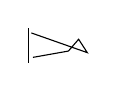
\begin{tikzpicture}
\draw (0,-.22)--(0,.22);
\draw (.04,.16)--(.75,-.09)--(.64,.08)--(.51,-.07)--(.06,-.15);
\end{tikzpicture}}}

% 492-03: display (50).
\[
(50)\qquad \unsure{\widetilde{\mathcal T}_{1,1}}
\longrightarrow \mathrm{GL}(2,\widehat{\mathbb Z})
\]

% 492-04: middle and lower paragraph.
et il faudrait \deleted{\unsure{pouvoir}} interpréter cet homomorphisme
comme l'homomorphisme fondamental ``modulaire'' de la théorie des courbes
elliptiques (que l'image inverse de \deleted{$\unsure{\Gamma}$}
$\Gamma_{\mathbb Q}\subset\widetilde\Gamma_{\mathbb Q}$ dans
$\unsure{\widetilde{\mathcal T}_{1,1}}$ \unsure{puisse} s'interpréter comme
$\unsure{\mathcal T_{1,1}}\simeq\pi_1(M_{1,1\,\mathbb Q})$
doit être plus ou moins tautologique, par construction.)

% 492-05: final paragraph, interlinear addition, and display (51).
Il est clair en tous cas que les deux coïncident
\inserted{pour tt $\gamma\in\widetilde M_{0,3}$}
\unsure{vus} \unsure{comme|quand} éléments de
\[
(51)\qquad \mu_2(\widehat{\mathbb Z})=\{\pm1\}^{\mathbb P}
\qquad (\mathbb P=\text{ens. des nbs. premiers})
\]
\mspage{491}
\scanpage{493}
\mspage{549}
% 493-01: continuation, with an overwritten source in the first display.
i.e. ils coïncident modulo un hom
\[
\deleted{\unsure{M_{0,3}}}\inserted{\unsure{\widetilde\Gamma_{\mathbb Q}}}
\longrightarrow\mu_2(\widehat{\mathbb Z})\simeq\{\pm1\}^{\mathbb P}
\]
i.e. un hom
\[
\begin{aligned}
G_{\mathrm m}(\widehat{\mathbb Z})_2
&=(\widehat{\mathbb Z}^{*})_2\simeq\{\pm1\}^{\mathbb P}
\longrightarrow\deleted{\unsure{\mu}}\unsure{{}_2G_{\mathrm m}}(\widehat{\mathbb Z})
=\mu_2(\widehat{\mathbb Z})\\
&\hspace{24em}\simeq\{\pm1\}^{\mathbb P}
\end{aligned}
\]

% 493-02: middle prose.
--- donc ce n'est pas une \unsure{certaine} ind. qui est en cause !
C'est moralement sûr que les deux coïncident --- je n'ai pas essayé de le
prouver.

% 493-03: lower prose and its interlinear insertion.
Quant à (35) (36), ils doivent correspondre sûrement à l'action de
$\Gamma_{\mathbb Q}$ sur les modules de Tate des courbes elliptiques à
isomorphismes exceptionnels, correspondant justement aux pts
$(1/2,2,-1)$ et $(-\overline{\mathrm j},-\mathrm j)$ de
$M_{0,3\,\mathbb Q}=M_{1,1}[2]'_{\mathbb Q}$.
L'indétermination de signe \inserted{\unsure{doit|dont}} \unsure{correspondre|correspond} à l'indétermination
à remonter un point de $M_{1,1}[2]'_{\mathbb Q}$ en un point de
$M_{1,1}[2]_{\mathbb Q}$, i.e. de choisir une courbe elliptique
(avec ``\uline{rigidification}'' d'échelon 2) correspondant aux données de
\uline{Legendre} $(0,1,\infty,\unsure{q|\rho})$ avec
$\unsure{\rho|q}=1/2$ ou $\unsure{\rho|q}=-\overline{\mathrm j}$.
\mspage{492}
\scanpage{494}
% 494-01: upper paragraph.
Même une fois que l'\unsure{ambiguité} de signe pour
$\Theta_{\unsure{G}}^{\unsure{\pi}}$ est levée en passant à l'extension
$\unsure{\widetilde{\mathcal T}_{1,1}}$ à deux feuillets de
$\widetilde M_{0,3}$, l'indétermination des signes pour
$\Theta_{\rho}^{\unsure{\pi}},\Theta_{\sigma}^{\unsure{\pi}}$
n'est pas \unsure{levée} pour autant, car les scindages
\deleted{$\unsure{\Psi_{\rho}^{\pi},\Psi_{\sigma}^{\pi}}$}
$\Psi_{1/2}^{\unsure{\pi}},\Psi_{-\overline{\mathrm j}}^{\unsure{\pi}}$)
ne sont pas pour autant des scindages ($\overline{\mathrm m}$ partiels !)
de \deleted{\unsure{cette}} \unsure{l'extension}
$\unsure{\widetilde{\mathcal T}_{1,1}}$, mais seulement de
$\widetilde M_{0,3}$ --- et les remonter en des scindages de
$\unsure{\widetilde{\mathcal T}_{1,1}}$
\inserted{sur $\unsure{\mathcal T_{1,1}}$,}
revient, très précisément, à choisir justement des courbes elliptiques à
rigidification de Legendre au dessus des pts $1/2,-\overline{\mathrm j}$.
Ainsi, des calculs faits en termes d'autom. des groupes à lacets
$\widehat\Pi_{0,3}$ \unsure{ou} \inserted{de}
$\unsure{\mathcal{C}}_{0,3}^{+\wedge}$,
\unsure{redonnent} \inserted{(sans les avoir \unsure{cherchés} !)}
des résultats qui collent de très près à des vérités arithmético-géométriques
particulièrement cruciales.
\mspage{493}
\scanpage{495}
\mspage{550}
% 495-01: heading.
49.\quad \uline{Homomorphismes de} $M_{0,3}$, les groupes
$M_{\rho,\sigma}$ généraux.

% 495-02: left-margin notes.
\margin{\unsure{Où on se met dans le bain}\ldots}
\margin{\unsure{Toute} cette section \inserted{I} \unsure{semble}
entièrement inutile pour la suite, c'est un \unsure{tâtonnement}
préliminaire pour déboucher sur la section \uline{II} p.553.}

% 495-03: first paragraph.
I) Considérons un sous-groupe \inserted{fermé} $G$ de $M_{0,3}$,
contenant $\unsure{\mathcal C}_{0,3}^{+\wedge}$, donc image inverse d'un
sous-groupe fermé de $\widetilde\Gamma_{0,3}$.
On suppose que celui-ci est ``suffisamment gros'' --- disons qu'il contienne
un sous-groupe d'indice fini de
$\Gamma_{\mathbb Q}\subset\widetilde\Gamma_{0,3}$.
Pour le moment, on suppose pour simplifier que $G\subset\operatorname{Ker}\varepsilon_3$.
En résumé
\[
(1)\qquad
\unsure{\mathcal C}_{0,3}^{+\wedge}\subset G\subset\widetilde M_{0,3},
\qquad u\in G\Longrightarrow\mu(u)\equiv1\ (3).
\]

% 495-04: interlinear correction and parallel maps.
Cette dernière hypothèse \deleted{implique}\inserted{signifie} donc que
pour tout $u\in G$, on a $\alpha_0(u)\in\unsure{\mathcal C}_{0,3}^{\wedge+}$,
donc on a
\[
(\unsure{2})\qquad
\diagram{\begin{tikzcd}[column sep=large]
G \arrow[r,shift left=.7ex,"\underline{\alpha}_0"]
  \arrow[r,shift right=.7ex,"\underline{\beta}_0"']
& \unsure{\mathcal C}_{0,3}^{+}
\end{tikzcd}},
\]
caractérisées par
\[
(2')\qquad
\left\{\begin{aligned}
u(\rho)&=\operatorname{int}(\alpha_0)\rho\\
u(\sigma)&=\operatorname{int}(\beta_0)\sigma
\end{aligned}\right.
\qquad
\begin{aligned}
\alpha_0&=\underline{\alpha}_0(u)\\
\beta_0&=\underline{\beta}_0(u).
\end{aligned}
\]

% 495-05: the vertically arranged subgroups, including the intervening sign.
On considère
\[
(3)\qquad
\begin{array}{l}
G(0)=G\cap\widetilde M_{0,3}(0)\\[-.4em]
\quad\cap\\[-.4em]
G[0]=G\cap\widetilde M_{0,3}[0]=\operatorname{Norm}_{G}(L_0^{\unsure{\mathcal C}})
\end{array}
\]
de sorte que
\[
\begin{aligned}
(4)\qquad&G=G(0).\unsure{\mathcal C}_{0,3}^{+\wedge}
&&\text{(produit semi-direct)}\\
(5)\qquad&G[0]=G(0).L_0^{\unsure{\mathcal C}}
&&\text{id}\\
(6)\qquad&G[0]\cap\unsure{\mathcal C}_{0,3}^{+\wedge}
=L_0^{\unsure{\mathcal C}}.
\end{aligned}
\]

% 495-06: definition (7) and last line.
On a posé
\[
(7)\qquad
\begin{gathered}
L_0^{\unsure{\mathcal C}}=\text{sous-groupe fermé de }
\unsure{\mathcal C}_{0,3}^{+\wedge}\text{ engendré}\\
\text{par }\varepsilon_0
\end{gathered}
\]
et on définit de $\overline{\mathrm m}$ $L_1^{\unsure{\mathcal C}},L_{\infty}^{\unsure{\mathcal C}}$.
\mspage{494}
\scanpage{496}
% 496-01: paragraph and first map, with changes of target notation.
Considérons un groupe \inserted{profini}
$\deleted{\unsure{A}}\inserted{M}$, et un hom \inserted{(continu)}
\uline{surjectif}
\[
(8)\qquad \varphi:G\longrightarrow\deleted{\unsure{A}}M.
\]
On pose
\[
(9)\quad
\left\{\begin{aligned}
\varphi(\unsure{\mathcal C}_{0,3}^{+\wedge})
 &=\unsure{\mathcal C}\qquad\text{ss-groupe distingué de }M\\
\varphi(G(0))&=\deleted{\unsure{A}}\inserted{M}(0)\\
\varphi(G[0])&=\deleted{\unsure{A}}\inserted{M}[0].\\
\varphi(L_0^{\unsure{\mathcal C}})&=L_0^{\deleted{\unsure{\mathcal C}}}
\end{aligned}\right.
\]

% 496-02: subgroup relations.
\deleted{\unsure{Donc}}

Donc ce sont des sous-groupes fermés de $M$, satisfaisant
\[
\begin{aligned}
(10)\qquad&M(0)\subset M[0]\subset\operatorname{Norm}_{M}(L_0)\\
(11)\qquad&L_0^{\deleted{\unsure{\mathcal C}}}
\subset\unsure{\mathcal C}\cap M[0].
\end{aligned}
\]

% 496-03: the surviving generator relations.
Par abus de langage, on désigne encore par $\rho,\sigma,\varepsilon_0,\varepsilon_1$
\ldots\ les images de ces éléments dans $\unsure{\mathcal C}$, qui y
satisfont donc les relations connues dans $\unsure{\mathcal C}_{0,3}^{+\wedge}$,
en particulier
\[
(12)\qquad
\sigma^2=\rho^3=1,\qquad
\sigma\rho=\varepsilon_0,\quad \rho\sigma=\varepsilon_1,\qquad
\varepsilon_1=\sigma(\varepsilon_0)=\rho(\varepsilon_0).
\]

% 496-04: paragraph and revised definition (13).
Les restrictions des applications $\alpha_0,\beta_0$ de (2,2') à
$M_{\rho,\sigma}[0]$ seront plutôt notées $\alpha,\beta$, où $\alpha,\beta$
sont en fait des applications
\[
(13)\quad
\diagram{\begin{tikzcd}[column sep=large]
{\begin{gathered}
SG\overset{\mathrm{dfn}}=\deleted{\text{extension de}}\ G\\
\text{par }L_0^{\unsure{\mathcal C}},\ \text{image}\\
\text{inverse de }\unsure{G}\\
\text{dans }S\widetilde M_{0,3}\\
=\{(u,f)\in G\times\unsure{\mathcal C}_{0,3}^{+\wedge}\mid fu\in G[0]
\end{gathered}}
\arrow[r,shift left=.7ex,"\alpha"]
\arrow[r,shift right=.7ex,"\beta"']
&\unsure{\mathcal C}_{0,3}^{+\wedge}
\end{tikzcd}}
\]
dont on regarde les restrictions au \uline{sous-groupe}
($\simeq M_{\rho,\sigma}[0]$) de $SG$ défini par la relation $f=1$.

% 496-05: composition of the two functions, and (14).
Composant $\underline\alpha,\underline\beta:$
\diagram{\begin{tikzcd}[column sep=small]
\deleted{\unsure{M[0]}}\inserted{G[0]}
\arrow[r,shift left=.5ex]\arrow[r,shift right=.5ex]
&\unsure{\mathcal C}_{0,3}^{+\wedge}
\end{tikzcd}}
avec $\varphi\mid\unsure{\mathcal C}_{0,3}^{+\wedge}$, on trouve des
applications, encore notées $\underline\alpha,\underline\beta$
(où $\underline\alpha^M,\underline\beta^M$ en cas de confusion possible)
\[
(14)\qquad
\diagram{\begin{tikzcd}[column sep=large]
G[0]\arrow[r,shift left=.7ex,"\underline\alpha"]
\arrow[r,shift right=.7ex,"\underline\beta"']
&\unsure{\mathcal C}
\end{tikzcd}}
\]
satisfaisant donc
\[
(15)\qquad
\left\{\begin{aligned}
\unsure{u}(\rho)&=\operatorname{int}(\alpha)\rho\\
\unsure{u}(\sigma)&=\operatorname{int}(\beta)\sigma
\end{aligned}\right.
\qquad
\begin{gathered}
\text{pour }u\in M[0]\ \inserted{\text{\unsure{de}}}\text{ la forme }\varphi(u_0),\\
\text{et }\alpha=\underline\alpha(u_0),\ \beta=\underline\beta(u_0).
\end{gathered}
\]
\mspage{495}
\scanpage{497}
\mspage{551}

% 497-01
A priori, $\alpha$ et $\beta$ dépendent du choix de $u_0$ dont $u$ provient
pas seulement de $u$ --- mais
% 497-02
\[
(16)\qquad
\left\{\begin{aligned}
\alpha\rho(\alpha)^{-1}&=[u,\rho]\\
\beta\sigma(\beta)^{-1}&=[u,\sigma]
\end{aligned}\right.
\]
% 497-03
n'en dépendent pas. Si on pose
% 497-04
\[
(17)\qquad
T_{\rho}=\uline{\mathrm{Centr}}_M(\rho)
\qquad
T_{\sigma}=\uline{\mathrm{Centr}}_M(\sigma)
\]
% 497-05
on voit donc que, modulo $T_{\rho}$ resp. $T_{\sigma}$,
$\alpha,\beta$ ne dépendent que de $u$.

% 497-06, 497-07, 497-08, 497-09
\uline{Hypothèse}
$\alpha\inserted{{}=\alpha(u_0)},\beta\inserted{{}=\beta(u_0)}$
ne dépendent que de $u=\varphi(u_0)$
(pour $u_0\in\deleted{\unsure{M}}\unsure{G}[0]$).

% 497-10
On va \unsure{exprimer} cette hypothèse de façon un peu différente,
en introduisant
% 497-11
\[
(18)\qquad J=\operatorname{Ker}(G[0]\longrightarrow M[0]),
\]
% 497-12, 497-13
on veut donc que pour $\deleted{\unsure{\alpha}}$
% 497-14, 497-15
\[
u'_0=\deleted{u_0}\delta_0u_0\quad
\text{avec }u_0\in G[0],\ \delta_0\in J,\quad\text{on ait}
\]
% 497-16
\[
\alpha(u'_0)=\alpha(u_0),\qquad \beta(u'_0)=\beta(u_0)
\]
% 497-17, 497-18
\unsure{Notons}
\[
\begin{gathered}
\alpha_0=\uline{\alpha}(u_0),\quad
\beta_0=\uline{\beta}(u_0),\quad
\alpha'_0=\uline{\alpha}(u'_0),\quad
\beta'_0=\uline{\beta}(u'_0),\quad
\overline{\alpha}_0=\uline{\alpha}(\delta_0),\quad
\overline{\beta}_0=\uline{\beta}(\unsure{\delta_1|\delta_0}),
\end{gathered}
\]
\uline{dans} $G$, de sorte qu'on aura, par les formules de cocycles de $G$
% 497-19
\[
\alpha'_0=\delta_0(\alpha_0)\overline{\alpha}_0,
\qquad
\beta'_0=\delta_0(\beta_0)\overline{\beta}_0,
\]
% 497-20
d'où, en appliquant $\varphi$ et notant que
% 497-21
\[
\begin{aligned}
\varphi(\delta_0(\alpha_0))
&=\underbrace{\varphi(\delta_0)}_{1}(\varphi(\alpha_0))
=\varphi(\alpha_0)\overset{\mathrm{dfn}}=\alpha
&&\text{et de }\overline{\mathrm m}\\
\varphi(\delta_0(\beta_0))&=\varphi(\beta_0)\overset{\mathrm{dfn}}=\beta
\end{aligned}
\]
% 497-22, 497-23
\[
(19)\qquad
\alpha'=\deleted{\unsure{\varphi}}\alpha\overline{\alpha},\qquad
\beta'=\beta\overline{\beta}\qquad\text{dans }\unsure{\mathcal{C}}
\]
% 497-24, 497-25
où $\alpha,\beta,\alpha',\beta',\overline{\alpha},\overline{\beta}$ sont les images par
$\varphi$ des quantités $\alpha_0$ etc dans $\unsure{\mathcal{C}}_{0,3}^{+\wedge}$.
\deleted{\unsure{avec} $\alpha=\alpha(u_0)$}
Donc l'hypothèse signifie ceci
% 497-26
\[
(20)\qquad
\forall\,\delta_0\in J\overset{\mathrm{dfn}}=
\operatorname{Ker}(G[0]\longrightarrow M[0]),\quad
\text{on a}\quad
\unsure{\alpha^{\Pi}}(\delta_0),\unsure{\beta^{\Pi}}(\delta_0)
\in\unsure{\operatorname{Ker}}\varphi
\]
% 497-27, 497-28
\deleted{\unsure{lorsque}}
Quand cette hypothèse est satisfaite, on a donc des applications
\mspage{496}
\scanpage{498}

% 498-01
\[
(21)\qquad
\diagram{\begin{tikzcd}[column sep=large]
M[0]\arrow[r,shift left=0.65ex,"\uline{\alpha}"]
\arrow[r,shift right=0.65ex,"\uline{\beta}"']&\unsure{\mathcal{C}}
\end{tikzcd}}
\]
% 498-02, 498-03
\deleted{satisfaisant}
\unsure{factorisant} (14), et satisfaisant donc
% 498-04
\[
(22)\qquad
\left\{\begin{aligned}
u(\rho)&=\operatorname{int}(\alpha)\rho\\
\unsure{u}(\sigma)&=\operatorname{int}(\beta)\sigma
\end{aligned}\right.
\qquad
\text{pour }\unsure{u}\in M[0],\quad
\alpha=\uline{\alpha}(u),\quad\beta=\uline{\beta}(u),
\]
% 498-05, 498-06, 498-07
qui \deleted{\unsure{généralisent|généralisant}}
\inserted{\unsure{paraphrasent}} (2').

% 498-08
D'ailleurs, posons
% 498-09
\[
(23)\qquad
\unsure{\zeta|\xi}=\alpha\rho(\alpha)^{-1},\qquad
\eta=\beta\sigma(\beta)^{-1}
\]
% 498-10
les relations (22) s'écrivent ainsi
% 498-11
\[
(24)\qquad u(\rho)=\unsure{\zeta|\xi}\rho,\qquad u(\sigma)=\eta\sigma
\]
% 498-12
et on aura
% 498-13
\[
(25)\qquad \unsure{\zeta|\xi}=[u,\rho],\qquad \eta=[u,\sigma]
\]
% 498-14
et de plus
% 498-15
\[
(26)\qquad
\unsure{\zeta|\xi}=\eta\unsure{\varepsilon_1|\ell_1}^{\nu}\qquad
\text{où }\nu=\frac{\mu-1}{2}\in\widehat{\mathbb Z}
\quad\text{($\mu$ le multiplicateur de $u$).}
\]
% 498-16
qui provient de la relation unique dans $\unsure{\mathcal{C}}_{0,3}^{+}$.

% 498-17
(On suppose pour fixer les idées que l'hom
% 498-18, 498-19
\[
\deleted{\unsure{(27)}}\qquad
\diagram{\begin{tikzcd}[column sep=large]
G\arrow[r,"\chi^{G}"]&\widehat{\mathbb Z}^{*}
\end{tikzcd}}
\qquad\text{(``multiplicateur'')}
\]
% 498-20
se factorise par
% 498-21
\[
(27)\qquad
\diagram{\begin{tikzcd}[column sep=large]
G\arrow[r]&M\arrow[r,"\chi^{M}"]&\widehat{\mathbb Z}^{*},
\end{tikzcd}}
\]
% 498-22
de sorte qu'on a une notion de multiplicateur ($\in\widehat{\mathbb Z}^{*}$)
pour les $u\in M$.)

% 498-23
Considérons l'hom naturel
% 498-24
\[
(28)\qquad
\diagram{\begin{tikzcd}[column sep=large,row sep=small]
M[0]\arrow[r]&\operatorname{Aut}(\unsure{\mathcal{C}}):\\
u\arrow[r,mapsto]&\operatorname{int}(u)|\unsure{\mathcal{C}}
\end{tikzcd}}
\]
% 498-25, 498-26
on voit sur (22) \inserted{\unsure{même|ou $\overline{\mathrm m}$} (24)}
qu'il est connu quand on connaît
\mspage{497}
\scanpage{499}
\mspage{552}

% 499-01, 499-02
\margin{car \deleted{\illegible{1}} $\rho,\sigma$ engendrent
\unsure{topolog$^t$} $\unsure{\mathcal{C}}$}
% 499-03
les fonctions $\uline{\alpha},\uline{\beta}:M[0]\longrightarrow\unsure{\mathcal{C}}$,
et $\overline{\mathrm m}$ quand on connaît seulement
$\unsure{\zeta|\xi},\eta:M[0]\longrightarrow\unsure{\mathcal{C}}$.
Si d'ailleurs on pose
% 499-04
\[
(29)\qquad
M'[0]=\operatorname{Im}(M[0]\longrightarrow\operatorname{Aut}(\unsure{\mathcal{C}}))
\]
% 499-05
ces dernières fonctions $\unsure{\zeta|\xi},\eta$ sont déjà définies sur $M'[0]$ --- alors qu'il
n'est pas clair qu'il en soit de $\overline{\mathrm m}$ de $\alpha,\beta$, quand
$M[0]$ \unsure{n'agit|n'opère} pas fidèlement sur $\unsure{\mathcal{C}}$.
On a ainsi une application \inserted{$(\unsure{\zeta|\xi},\eta)$} d'un certain sous-groupe
$M'[0]\subset\operatorname{Norm}_{\operatorname{Aut}(\unsure{\mathcal{C}})}(L_0)$
dans l'ens $\unsure{\mathcal{R}}$ des solutions de l'équation en $\unsure{\zeta|\xi},\eta$
(26) qu'on \unsure{écrit|écrira} simplement
% 499-06
\[
(30)\qquad \eta^{-1}\unsure{\zeta|\xi}\in L_1
\]
% 499-07, 499-08
relation qui implique (26) (avec la forme précise de l'exposant $\nu$)
si on suppose \inserted{(\unsure{p.ex.})} $\unsure{\mathcal{C}|M}$ assez gros pour que
% 499-09
\inserted{$\diagram{\begin{tikzcd}[column sep=large]
\unsure{\mathcal{C}}_{0,3}^{+\wedge}\arrow[r,"\unsure{2}"']&
\unsure{\mathrm{SL}|\mathrm{PSL}}(2,\widehat{\mathbb Z})
\end{tikzcd}}$}
se factorise par $\unsure{\mathcal{C}}$ --- ce qu'on va supposer, pour nous simplifier la vie.

% 499-10, 499-11
\deleted{On va faire sur $\unsure{\mathcal{C}}$, muni de $\rho,\sigma,\varepsilon_1$
l'hypothèse suivante}
\inserted{De façon plus précise, soit}
% 499-12
\deleted{(31) \unsure{H)|II)} Sur}
% 499-13, 499-14, 499-15, 499-16
\[
(32)\qquad
\left\{\begin{gathered}
\deleted{\unsure{\Sigma|\mathcal{R}}}\ \unsure{=}
\Sigma_{\unsure{\mathcal{C}},\rho,\sigma}
\subset\unsure{\mathcal{C}}\times\unsure{\mathcal{C}}\\
\Vert\\[-1ex]
\left\{(\unsure{\zeta|\xi},\eta)\ \middle|
\begin{array}{ll}
\text{a)}&\unsure{\zeta|\xi}\rho\ \text{conjugué à }\rho\quad
\deleted{\text{dans }\operatorname{Aut}(\unsure{\mathcal{C}})}
\inserted{\text{dans }\unsure{\mathcal{C}}}\\[1ex]
\text{b)}&\eta\sigma\quad\rule{2.7cm}{0.4pt}\quad\sigma\quad\rule{2cm}{0.4pt}\\[1ex]
\text{c)}&\eta^{-1}\unsure{\zeta|\xi}\in L_1\quad\text{i.e.}\quad
\exists\nu'\in\widehat{\mathbb Z}\ \text{que }\unsure{\zeta|\xi}=\eta\varepsilon_1^{\nu'}
\end{array}\right\}
\end{gathered}\right.
\]
% 499-17, 499-18
\margin{\[
\begin{gathered}
\underbrace{[\alpha,\rho]=\alpha\rho(\alpha)^{-1}}\\
\left\{\begin{array}{l}
\text{\unsure{i.e.} }\unsure{\zeta|\xi}\ \text{\unsure{de la forme} }\unsure{[\alpha,\rho]}\\
\text{\unsure{resp.} }\eta\ \text{\unsure{de la forme} }\unsure{[\beta,\sigma]}
\unsure{{}=\beta\sigma(\beta)^{-1}}
\end{array}\right.
\end{gathered}
\]}

% 499-19, 499-20, 499-21, 499-22, 499-23
\deleted{Pour \unsure{tt} $u\in\operatorname{Aut}(\unsure{\mathcal{C}})$
\uline{normalisant} $L_0$, \deleted{et \unsure{fixant}}
\deleted{\unsure{doivent}} et fixant la classe de conjugaison de
$\rho$ et celle de $\sigma$, i.e. \unsure{telle|tel} que
\[
\deleted{\unsure{\zeta|\xi}=[u,\rho]}\qquad(\unsure{\zeta|\xi},\eta)=([u,\rho],[u,\sigma])
\]
\unsure{satisfassent|satisfasse} aux deux premières conditions de (33), \unsure{et}}
\mspage{498}
\scanpage{500}

% 500-01
et soit $u\in\operatorname{Aut}(\unsure{\mathcal{C}})$ un automorphisme de
$\unsure{\mathcal{C}}$, et posons
% 500-02
\[
(34)\qquad
\left\{\begin{aligned}
\unsure{\zeta|\xi}&=[u,\rho]=u\rho u^{-1}\rho^{-1}=u(\rho)\rho^{-1}
&&\text{i.e. }u(\rho)=\unsure{\zeta|\xi}\rho\\
\eta&=[u,\sigma]=u(\sigma)\sigma^{-1}
&&\text{i.e. }u(\sigma)=\eta\sigma
\end{aligned}\right.
\]
% 500-03
\margin{cf (24),(25)}
% 500-04, 500-05, 500-06
alors dire que $\unsure{\zeta|\xi}\rho$ \inserted{$(=u(\rho))$} est conjugué à $\rho$ signifie
que $u$ fixe la classe de conj. de $\rho$, dire que $\eta\sigma$
\inserted{$(=u(\sigma))$} est conjugué \unsure{de|à} $\sigma$ signifie que $u$ fixe
la classe de conj. de $\sigma$.
Enfin la condition $\eta^{-1}\unsure{\zeta|\xi}\in L_1$ s'écrit aussi, comme
% 500-07, 500-08
\[
\begin{aligned}
\eta^{-1}\unsure{\zeta|\xi}
&=(\sigma u(\sigma^{-1}))(u(\rho)\rho^{-1})
=\sigma u(\sigma^{-1}\rho)\rho^{-1}\\
&=\sigma\left(u(\underbrace{\sigma^{-1}\rho}_{\varepsilon_0})
\deleted{\unsure{\sigma}}\underbrace{\rho^{-1}\sigma}_{\varepsilon_0^{-1}}\right)
\end{aligned}
\]
% 500-09
\margin{NB $\sigma^{-1}=\sigma$}
% 500-10, 500-11
\deleted{\unsure{d'où}}
\[
{}=\sigma(u(\varepsilon_0)\varepsilon_0^{-1})
\]
% 500-12
sous la forme
% 500-13
\[
\sigma(u(\varepsilon_0)\varepsilon_0^{\unsure{-1}})\in L_1
\qquad\text{i.e.}\qquad
u(\varepsilon_0)\varepsilon_0^{-1}\in L_0
\]
% 500-14, 500-15, 500-16
(puisque $L_0=\sigma^{-1}(L_1)$) ou encore
(puisque $\varepsilon_0$ \deleted{engendre}\inserted{$\in L_0$})
% 500-17
\[
u(\varepsilon_0)\in L_0,\quad
\text{soit (puisque $\varepsilon_0$ engendre $L_0$)}
\]
% 500-18
\margin{Dans cet argument, on n'a utilisé que la relation
$\sigma^{-1}\rho=\varepsilon_0$ et le fait que $\varepsilon_0$ engendre $L_0$,
\unsure{et pas} que $\sigma^2=1$ ou $\rho^3=1$ p.ex.}
% 500-19
\[
u(L_0)=L_0
\]
% 500-20
i.e. que $u$ \uline{normalise} $L_0$.

% 500-21
Soit donc
% 500-22
\[
(35)\qquad
\left\{\begin{gathered}
\widetilde{B}'_0\subset\operatorname{Aut}(\unsure{\mathcal{C}})\\
\Vert\ \mathrm{dfn}\\[-1ex]
\left\{u\in\operatorname{Aut}(\unsure{\mathcal{C}})\ \middle|
\begin{array}{l}
u\ \text{fixe \unsure{cl.} de conj. de $\rho$ et celle de $\sigma$}\\
u\ \text{normalise }L_0
\end{array}\right\},
\end{gathered}\right.
\]
% 500-23
de sorte qu'on a une application (injective parce que $\rho,\sigma$ engendrent
$\unsure{\mathcal{C}}$)
% 500-24
\[
(36)\qquad
\diagram{\begin{tikzcd}[column sep=large,row sep=small]
\widetilde{B}'_0\arrow[r,hook]&\Sigma\\
u\arrow[r,mapsto]&([u,\rho]=u(\rho)\rho^{-1},\ [u,\sigma]=u(\sigma)\sigma^{-1}).
\end{tikzcd}}
\]
\mspage{499}
\scanpage{501}
\mspage{553}

% 501-01--07: heading, double marginal rule, hypothesis and its alterations.
\[
(37)\quad
\begin{array}{||l}
\text{\uline{Hypothèse fondamentale sur} }\unsure{\mathcal{C}},\ 
\text{\uline{muni de} }\rho,\sigma,\ 
\text{\deleted{et}\inserted{\uline{d'où}} }\varepsilon_0=\sigma^{-1}\rho,\\[1ex]
\varepsilon_1=\rho\sigma^{-1}=\sigma(\varepsilon_0)=\rho(\varepsilon_0):\\[1ex]
\text{a) }\unsure{\mathcal{C}}\text{ est engendré topologiquement par }\rho,\sigma\\[1ex]
\text{b) L'application (36) \deleted{\unsure{est|par}} (injective par a)) est}\\
\text{\phantom{b) }bijective.}
\end{array}
\]

% 501-08--10: canceled first version and its replacement.
\deleted{Cela signifie donc que $\forall(\unsure{\zeta|\xi},\eta)\in\Sigma$ \unsure{est|u}}

La condition b) signifie donc que pour
\deleted{de la forme $u$,}
$(\alpha,\beta)\in\unsure{\mathcal{C}}\times\unsure{\mathcal{C}}$,
satisfaisant une relation
\[
\uline{\alpha\rho(\alpha)^{-1}}
=\uline{\beta\sigma(\beta)^{-1}}\varepsilon_1^{\nu'},
\qquad \unsure{\nu''|\nu'}\text{ convenable},
\]
il existe $u\in\operatorname{Aut}(\unsure{\mathcal{C}})$ tel qu'on ait
% 501-12--14: two identities, including the canceled right-hand attempt.
\[
\begin{array}{lll}
[u,\rho]=\alpha\rho(\alpha)^{-1}&
\text{i.e. }u(\rho)=\operatorname{int}(\alpha)(\rho)&
\text{i.e. }\inserted{\unsure{u(\rho)|u\rho)}=\unsure{\zeta|\xi}\rho}
\deleted{\unsure{\operatorname{int}(\unsure{\zeta|\xi})\rho}}\\[1ex]
[u,\sigma]=\beta\sigma(\beta)^{-1}&
\text{i.e. }u(\sigma)=\operatorname{int}(\beta)\sigma&
\text{i.e. }u(\sigma)=\eta\sigma
\end{array}
\]

% 501-15: prose continuation (tilde is not visible on this B).
\margin{$\unsure{\bullet}$}
(on aura donc nécessairement $u\in B'_0\ \unsure{\}}$, et
$u$ sera unique si \unsure{on a} a)).

% 501-16--18: final paragraph and overwritten subscript.
Ainsi, sur l'ens. \unsure{des|de} $\unsure{R|\mathcal{R}}_{\rho,\sigma}$ des $(\unsure{\zeta|\xi},\eta)$ satisfaisant
a) b) c), on aura une structure de groupe, \unsure{+|et} \unsure{déduite|décrite} par transport de structure de celle de
$\widetilde{B}'_{\deleted{\unsure{\rho}}0}$

\unsure{etc.}

\mspage{500}
\scanpage{502}
\margin{\uline{Les groupes} $M_{\rho,\sigma}$ \uline{etc}}

II Reprenons la situation ci dessus, en oubliant (au moins pour le moment) $G$, $\varphi$ etc.

\margin{Pour une rectification \unsure{systématique} des notations \unsure{qui suivent|suivantes} cf p. 564, \uline{remarque}.}

Soit $\unsure{\mathcal{C}}$ un groupe --- on se place, pour ce qui suit, soit dans la cat. des groupes discrets, soit dans celle des groupes profinis, au choix. On va (pour fixer les idées) prendre celle des groupes profinis. On suppose donnés
\[
(1)\qquad \rho,\sigma\in\unsure{\mathcal{C}}
\]
\margin{[\unsure{i.e. on a entre} $\varepsilon_0=\ell'_0$, $\sigma=\ell'_1$ et $\rho^{-1}=\ell'_\infty$ avec relation (2) $\ell'_\infty\ell'_1\ell'_0=1$]}
on pose
\[
\varepsilon_0=\sigma^{-1}\rho,\qquad
\varepsilon_1=\rho\sigma^{-1}=\sigma(\varepsilon_0)=\rho(\varepsilon_0)
\]
\[
(3)\qquad
\begin{aligned}
L_0&=\text{sous-groupe fermé engendré par }\varepsilon_0\\
L_1&=\rule{6.5cm}{0.3pt}\quad\varepsilon_1
\end{aligned}
\qquad\unsure{\text{, i.}}
\]
donc $L_1=\rho(L_0)=\sigma(L_0)$.

On \deleted{suppose} considère
\diagram{\begin{tikzcd}
\mathrm{Aut}(\unsure{\mathcal{C}}) \arrow[r,"\Phi=(\underline{\unsure{\zeta|\xi}},\underline{\eta})","\deleted{\unsure{\varphi}}"'] & \deleted{\unsure{\mathcal{C}}}\,\unsure{\mathcal{C}}\times\unsure{\mathcal{C}}
\end{tikzcd}}\hfill(4)
défini par
\[
(5)\quad
\left\{\begin{aligned}
\underline{\unsure{\zeta|\xi}}(u)&=[u,\rho]=u\rho u^{-1}\rho^{-1}=u(\rho)\rho^{-1}
&&\text{donc }u(\rho)=\unsure{\zeta|\xi}\rho\quad(\unsure{\zeta|\xi}=\underline{\unsure{\zeta|\xi}}(u))\\
&=u\rho(u)^{-1}\\
\underline{\eta}(u)&=[u,\sigma]=u\sigma u^{-1}\sigma^{-1}=u(\sigma)\sigma^{-1}
&&\text{donc }u(\sigma)=\eta\sigma\quad(\eta=\underline{\eta}(u))\\
&=u\sigma(u)^{-1}.
\end{aligned}\right.
\]
Donc pour $u\in\mathrm{Aut}(\unsure{\mathcal{C}})$, et $\unsure{\zeta|\xi}=\underline{\unsure{\zeta|\xi}}(u)$, $\eta=\underline{\eta}(u)$, on a
\[
\unsure{(6)|(5)}\quad
\left\{\begin{aligned}
&u\text{ fixe la classe de }\inserted{\unsure{\mathcal{C}}}\text{-conj. de }\rho
\quad\Longleftrightarrow\quad \unsure{\zeta|\xi}\rho\text{ conjugué à }\rho\\
&\hspace{6cm}\Longleftrightarrow\quad\unsure{\zeta|\xi}=\alpha\rho(\alpha)^{-1}\quad(\alpha\in\unsure{\mathcal{C}})\\
&u\text{ fixe la classe de }\unsure{\mathcal{C}}\text{-conj. de }\sigma
\quad\Longleftrightarrow\quad \eta\sigma\text{ conjugué à }\sigma\\
&\hspace{6cm}\Longleftrightarrow\quad\eta=\beta\sigma(\beta)^{-1}\quad(\beta\in\unsure{\mathcal{C}})\\
&u\text{ normalise }L_0\quad\Longleftrightarrow\quad\eta^{-1}\unsure{\zeta|\xi}\in L_1
\quad\Longleftrightarrow\quad\unsure{\zeta|\xi}=\eta\varepsilon_1^\nu\quad\text{avec }\nu\in\widehat{\mathbb Z}\text{ convenable}.
\end{aligned}\right.
\]
\mspage{501}
\scanpage{503}
\mspage{554}
\unsure{Soient|Soit} \deleted{$\unsure{B_{\rho,\sigma}}\subset$}
\[
(7)\qquad
\begin{aligned}
B_{\rho,\sigma}&\subset\mathrm{Aut}(\unsure{\mathcal{C}})\\[-2pt]
\Vert\quad&\\[-10pt]
\{u\mid{}&\text{satisfaisant les trois conditions }(\unsure{6|5})\}
\end{aligned}
\]
\[
(8)\qquad
\begin{gathered}
\Sigma_{\rho,\sigma}\subset\unsure{\mathcal{C}}\times\unsure{\mathcal{C}}\\[-2pt]
\Vert\\[-2pt]
\left\{(\unsure{\zeta|\xi},\eta)\ \middle|\ 
\begin{aligned}
\unsure{\zeta|\xi}&=\alpha\rho(\alpha)^{-1},\quad
\eta=\beta\sigma(\beta)^{-1}\quad(\alpha,\beta\in\unsure{\mathcal{C}})\\
&\inserted{\text{i.e. }\unsure{\zeta|\xi}\rho\text{ conj. à }\rho,\qquad\text{i.e. }\eta\sigma\text{ conj. à }\sigma}\\
\eta^{-1}\unsure{\zeta|\xi}&\in L_1\quad\text{i.e. }\unsure{\zeta|\xi}=\eta\varepsilon_1^\nu\quad(\nu\in\widehat{\mathbb Z})
\end{aligned}\right\},
\end{gathered}
\]
de sorte que $B_{\rho,\sigma}$ est l'image inverse de $\Sigma_{\rho,\sigma}$ par (4), et on a une application induite
\diagram{\begin{tikzcd}
B_{\rho,\sigma}\arrow[r,"\varphi=\varphi_{\rho,\sigma}"]&\Sigma_{\rho,\sigma}.
\end{tikzcd}}\hfill(9)

On suppose
\[
(10)\qquad\boxed{\left\{\begin{aligned}
\text{a)}\quad&\rho,\sigma\text{ engendrent }\unsure{\mathcal{C}}\text{ topologiquement}\\
\text{b)}\quad&\text{l'application (9) (injective par a))}\\
&\text{est surjective (donc bijective).}
\end{aligned}\right.}
\]
\margin{Attention, cette condition \uline{est} \deleted{\unsure{pas}} satisfaite pour $\unsure{\mathcal{C}}=\mathrm{SL}(2,\widehat{\mathbb Z})'$ ! (\unsure{elle impose} \deleted{\unsure{une condition de possibilité}} $\varepsilon=\varepsilon_3(\mu)$ \unsure{au groupe} $\unsure{\gamma}$ \unsure{en écrivant} $\unsure{\zeta|\xi},\unsure{\eta}$\dots)}

On transporte alors par $\varphi$ la structure de groupe de $B_{\rho,\sigma}$ à $\Sigma_{\rho,\sigma}$. On \deleted{désignera par}\inserted{pose}
\deleted{$u_{\unsure{\zeta|\xi},\eta}=\varphi^{-1}(\unsure{\zeta|\xi},\eta)$, pour}
\[
(11)\qquad u_{\unsure{\zeta|\xi},\eta}=\varphi^{-1}(\unsure{\zeta|\xi},\eta)\in B_{\rho,\sigma}
\qquad((\unsure{\zeta|\xi},\eta)\in\Sigma_{\rho,\sigma}),
\]
de sorte qu'\deleted{\unsure{on aura}} $u_{\unsure{\zeta|\xi},\eta}$ est caractérisé par
\[
(12)\qquad\left\{\begin{aligned}
u_{\unsure{\zeta|\xi},\eta}(\rho)&=\unsure{\zeta|\xi}\rho\\
u_{\unsure{\zeta|\xi},\eta}(\sigma)&=\eta\sigma
\end{aligned}\right.
\]
L'hypothèse b) signifie donc que, dès que $(\unsure{\zeta|\xi},\eta)\in\Sigma_{\rho,\sigma}$ i.e. $\unsure{\zeta|\xi}\rho$ conj. à $\rho$, $\eta\sigma$ conj. à $\sigma$ et $\eta^{-1}\unsure{\zeta|\xi}\in L_1$, il existe
\mspage{502}
\scanpage{504}
un autom. $u_{\unsure{\zeta|\xi},\eta}$ de $\unsure{\mathcal{C}}$ satisfaisant (12) (et qui sera unique par (10) a)). La loi de groupe sur $\Sigma_{\rho,\sigma}$ s'explicite ainsi :
\[
(13)\quad(\unsure{\zeta|\xi}',\eta')(\unsure{\zeta|\xi},\eta)=(\unsure{\zeta|\xi}'',\eta'')\quad\text{avec}\quad
\left\{\begin{aligned}
\unsure{\zeta|\xi}''&=u_{\unsure{\zeta|\xi}',\eta'}(\unsure{\zeta|\xi})\unsure{\zeta|\xi}'\\
\eta''&=u_{\unsure{\zeta|\xi}',\eta'}(\eta)\eta'.
\end{aligned}\right.
\]
Considérons l'hom \deleted{$g\mapsto\mathrm{int}(g)$}
\deleted{\unsure{Introduisons}} \deleted{Soit}
\diagram{\begin{tikzcd}
\unsure{\mathcal{C}}\arrow[r]&\mathrm{Aut}(\unsure{\mathcal{C}})\\
g\arrow[r,mapsto]&\mathrm{int}(g)
\end{tikzcd}}
et l'image inverse de $B_{\rho,\sigma}$ n'est autre que le normalisateur de $L_0$ dans $\unsure{\mathcal{C}}$, soit $N_0$. On veut construire alors un groupe $G_{\rho,\sigma}$, contenant $\unsure{\mathcal{C}}$ \inserted{comme un sous-groupe invariant} et dans lequel \deleted{$\unsure{B_{\rho,\sigma}}$} s'envoie $B_{\rho,\sigma}$, de façon que l'action tautologique de $B_{\rho,\sigma}$ sur $\unsure{\mathcal{C}}$ soit déduite de cet homomorphisme, et que $G_{\rho,\sigma}$ soit engendré par $\unsure{\mathcal{C}}$ et l'image de $B_{\rho,\sigma}$, notée $B'_{\rho,\sigma}$, qui contiendra \deleted{\unsure{donc}} $N_0$.

\deleted{\unsure{Pour|P.}}\inserted{\unsure{Si}} le centre de $\unsure{\mathcal{C}}$ est trivial i.e.
\diagram{\begin{tikzcd}
\unsure{\mathcal{C}}\arrow[r,hook]&\mathrm{Aut}(\unsure{\mathcal{C}})
\end{tikzcd}}
($\unsure{\mathcal{C}}$ sous-gr. dist),
\deleted{faire cette construction, partons de
\[
B_{\rho,\sigma}\cdot\unsure{\mathcal{C}}\qquad(\text{produit }\tfrac12\text{ direct})
\]
et considérons l'application}
\diagram{\begin{tikzcd}
\deleted{N_0}\arrow[r]&\deleted{B_{\rho,\sigma}\cdot\unsure{\mathcal{C}}}\\
\deleted{g}\arrow[r,mapsto]&\deleted{(\mathrm{int}(g),g^{-1})}
\end{tikzcd}}
il suffit de prendre le ss-groupe $G_{\rho,\sigma}$ de $\mathrm{Aut}(\unsure{\mathcal{C}})$ engendré par $\unsure{\mathcal{C}}$ et $B_{\rho,\sigma}$.

\deleted{Donc $N_0$ \unsure{est|a} \unsure{commutatif}, \unsure{mais}}
Mais l'hypothèse que le centre de $\unsure{\mathcal{C}}$ \unsure{soit|est} trivial n'est pas heureuse --- p.ex. elle n'est pas satisfaite si $\unsure{\mathcal{C}}=\mathrm{SL}(2,\widehat{\mathbb Z})/\pm1$.
Il me semble que l'introduction de $N_0$ (sur lequel en pratique nous n'avons aucun contrôle)
\mspage{503}
\scanpage{505}
\mspage{555}
n'était pas non plus judicieuse, et \deleted{que} la condition $B'_{\rho,\sigma}\supset N_0$ --- il suffit de $B'_{\rho,\sigma}\supset L_0$.
Je vais donc considérer
\[
(14)\quad\left\{\begin{gathered}
S_0G_{\rho,\sigma}\overset{\mathrm{dfn}}{=}B_{\rho,\sigma}\cdot\unsure{\mathcal{C}}\qquad\text{le produit }\tfrac12\text{ direct, et}
\end{gathered}\right.
\]
\diagram{\begin{tikzcd}
L_0\arrow[r,hook,"i"]&\deleted{B_{\rho,\sigma}\cdot\unsure{\mathcal{C}}}\ S_0G_{\rho,\sigma}\\
g\arrow[r,mapsto]&\mathrm{int}(g^{\unsure{\mathcal{C}}})\cdot g^{-1}
\end{tikzcd}}
l'image de cet homomorphisme est un sous-groupe \unsure{distingué}, car a) il commute à $\unsure{\mathcal{C}}$ (trivial) et b) il est invariant par $B_{\rho,\sigma}$, car on aura pour $u\in B_{\rho,\sigma}$
\[
\mathrm{int}(u)(i(g))=\mathrm{int}(u)(\mathrm{int}(g)\cdot g^{-1})
=\mathrm{int}(u(g))\cdot\underbrace{\mathrm{int}(u)(g^{-1})}_{u(g^{-1})=u(g)^{-1}}
=i(u(g))
\]
(i.e. $i$ commute aux actions de $B_{\rho,\sigma}$, opérant sur $L_0$ par restriction à $L_0$ de l'op. \inserted{\unsure{tautol.|totale}} de $B_{\rho,\sigma}$ sur $\unsure{\mathcal{C}}$, et sur \deleted{$B_{\rho,\sigma}\cdot\unsure{\mathcal{C}}$}\inserted{$S_0G_{\rho,\sigma}$} $\supset B_{\rho,\sigma}$ par autom. intérieurs).

On peut donc considérer
\[
(15)\qquad G_{\rho,\sigma}\overset{\mathrm{dfn}}{=}S_0G_{\rho,\sigma}/i(L_0)
\]
alors les hom d'inclusion
\diagram{\begin{tikzcd}
B_{\rho,\sigma}\arrow[r,hook]&S_0G_{\rho,\sigma}
\end{tikzcd}},
\diagram{\begin{tikzcd}
\unsure{\mathcal{C}}\arrow[r]&S_0G_{\rho,\sigma}
\end{tikzcd}}
donnent, par composition avec
\diagram{\begin{tikzcd}
S_0G_{\rho,\sigma}\arrow[r]&G_{\rho,\sigma}
\end{tikzcd}},
des hom
\diagram{\begin{tikzcd}
\deleted{\unsure{B_{\rho,\sigma}}}\unsure{\mathcal{C}}\arrow[r,"{\deleted{\unsure{\lhook}}}"{pos=0.08}]&G_{\rho,\sigma}
\end{tikzcd}},
\diagram{\begin{tikzcd}
B_{\rho,\sigma}\arrow[r,hook]&G_{\rho,\sigma}
\end{tikzcd}}\hfill(16)
rendant commutatif le diagramme
\diagram{\begin{tikzcd}[column sep=small,row sep=small]
&\unsure{\mathcal{C}}\arrow[dr,"{\deleted{\unsure{\lhook}}}"{pos=0.08}]&\\
L_0\arrow[ur,hook]\arrow[dr]&&G_{\rho,\sigma}\\
&B_{\rho,\sigma}\arrow[ur,hook]&
\end{tikzcd}}\hfill(17)
On note
\[
(18)\qquad\mathrm{Ker}(\unsure{\mathcal{C}}\longrightarrow G_{\rho,\sigma})
=L_0\cap\mathrm{Centr}(\unsure{\mathcal{C}})
=\mathrm{Ker}(L_0\longrightarrow B_{\rho,\sigma})
\]
\mspage{504}
\scanpage{506}
Dans le cas $\unsure{\mathcal{C}}=\mathrm{SL}(2,\widehat{\mathbb Z})'$, (avec $\rho,\sigma$ comme à l'accoutumée) on aura $L_0\cap\mathrm{Centr}(\unsure{\mathcal{C}})=\{1\}$. Donc il ne semble pas à priori qu'il y ait des inconvénients majeurs à supposer que
\[
(18)\qquad L_0\cap\mathrm{Centr}(\unsure{\mathcal{C}})=\{1\}\quad\text{i.e.}
\]
\diagram{\begin{tikzcd}
\unsure{\mathcal{C}}\arrow[r,hook]&\unsure{G}_{\rho,\sigma}\quad\text{inj.}
\end{tikzcd}}
Notons que \deleted{$L_0$ \unsure{va être|en est}} l'image de
\diagram{\begin{tikzcd}[row sep=small]
L_0\arrow[r]&B_{\rho,\sigma}\\
\ell\arrow[r,mapsto]&\operatorname{int}(\ell)
\end{tikzcd}}
(composé de (14) et de la projection $S_0G_{\rho,\sigma}\longrightarrow B_{\rho,\sigma}$) est évidemment \unsure{invariante|invariant}, et posant
\[
(19)\qquad\unsure{\Gamma_{\rho,\sigma}^{*}|\gamma_{\rho,\sigma}}=B_{\rho,\sigma}/\operatorname{Im}L_0
\]
on trouve
\[
(20)\qquad G_{\rho,\sigma}/\unsure{\mathcal{C}}_{\rho,\sigma}\simeq B_{\rho,\sigma}/L_0\simeq\unsure{\Gamma|\gamma}_{\rho,\sigma}.
\]
\margin{i.e. hom. de suites exactes
\diagram{\begin{tikzcd}[column sep=small,row sep=small]
1\arrow[r]&\deleted{\unsure{\mathcal{C}_{\rho,\sigma}}}\,L_0\arrow[r]\arrow[d]&B_{\rho,\sigma}\arrow[r]\arrow[d]&\unsure{\Gamma|\gamma}_{\rho,\sigma}\arrow[r,dash]\arrow[d,equal]&1\\
1\arrow[r]&\unsure{\mathcal{C}}\arrow[r]\arrow[d,equal]&G_{\rho,\sigma}\arrow[r]&\unsure{\Gamma|\gamma}_{\rho,\sigma}\arrow[r,dash]&1\\
&\unsure{SG_{\rho,\sigma}}&&&
\end{tikzcd}}(20bis)}

(\uline{NB} Dans le cas $\unsure{\mathcal{C}}=\mathrm{SL}(2,\widehat{\mathbb Z})'$ ; \deleted{$\unsure{B_{\rho,\sigma}}$} \unsure{etc.|et}, $B_{\rho,\sigma}$ \inserted{$\subset\unsure{\mathrm{GP}}(\widehat{\mathbb Z})$} est le groupe noté précédemment $B'_0$ (ou plutôt son image isomorphique $\widetilde B'_0$), et l'hom. $\mathrm{dét}\mid B'_0=B_{\rho,\sigma}$ \deleted{induit} (trivial sur $L_0$) induit par passage au quotient un \uline{isomorphisme}
\diagram{\begin{tikzcd}
\unsure{\Gamma|\gamma}_{\rho,\sigma}\arrow[r,"\sim"]&G_{\mathrm m}
\end{tikzcd}}\hfill(21)
\margin{Dans le cas où on part de $\mathrm{SL}(2,\widehat{\mathbb Z}),\rho,\sigma$, on tombe sur $G=\mathrm{GL}(2,\widehat{\mathbb Z})$\dots}
et on voit, \deleted{par} utilisant l'isomorphisme
\[
B'_0=\unsure{\widetilde T_0|\widetilde\Gamma_0}\cdot L_0\quad(\tfrac12\text{ direct})
\]
\inserted{où $\unsure{\widetilde T_0|\overline T_0}\xrightarrow{\sim}B'_0/L_0\simeq G_{\mathrm m}$}
\[
\text{i.e.}\qquad B_{\rho,\sigma}\simeq\unsure{\Gamma|\gamma}_{\rho,\sigma}\cdot L_0,
\]
que dans ce cas on a
\mspage{\unsure{505}}
\[
(22)\qquad G_{\rho,\sigma}=\deleted{\unsure{\mathrm{GL}}}\mathrm{GL}(2,\widehat{\mathbb Z})'.
\]
\mspage{505}
\scanpage{507}
\mspage{556}

Mais dans les cas plus généraux auxquels nous aspirons, il ne faut pas du \unsure{tt} s'attendre à ce que $\unsure{\Gamma}_{\rho,\sigma}$ soit aussi petit --- p.ex. qu'il soit commutatif.
Par exemple dans le cas ``universel'', $\unsure{\mathcal{C}}=\unsure{\mathcal{C}}_{0,3}^{+\wedge}$, on aura
\[
\tag{23}
B_{\rho,\sigma}=\widetilde{M}_{0,3}[0]'=
\operatorname{Ker}\bigl(\widetilde{M}_{0,3}[0]\xrightarrow{\varepsilon_3}\{\pm1\}\bigr)
\]
donc
\[
\tag{24}
\unsure{\Gamma}_{\rho,\sigma}\simeq\widetilde{\Gamma}_{0,3}'
\quad(\supset\Gamma_{\mathbb{Q}}'\ !).
\]

Par contre, on doit pouvoir sans inconvénient postuler l'existence d'un scindage \inserted{canonique} de l'extension $B_{\rho,\sigma}$ de $\Gamma_{\rho,\sigma}$ par $L_0$.
En fait, si on suppose, \deleted{$\unsure{\mathcal{C}}$ \unsure{quelconque}} \deleted{\unsure{que} \illegible{1} \unsure{est}}
\unsure{dans} le cas général, où néanmoins on suppose $\sigma^2=\rho^3=1$, i.e. $\unsure{\mathcal{C}}$ quotient de $\unsure{\mathcal{C}}_{0,3}^{+\wedge}$, que le quotient $\unsure{\mathcal{C}}$ de $\unsure{\mathcal{C}}_{0,3}^{+\wedge}$ est assez grand pour s'envoyer dans $\unsure{\mathrm{GP}|\mathrm{CP}}(\widehat{\mathbb{Z}})$, alors \deleted{\unsure{que le}} $B_{\rho,\sigma}\simeq\Sigma_{\rho,\sigma}$ s'envoie dans $\unsure{\widetilde{B}'_{0,3}|\widetilde{B}'_{0}}$, et l'image inverse de $\widetilde{T}_0$ est un sous-groupe (\unsure{qu'on pourrait} noter $T_{\rho,\sigma}$)
\[
\tag{25}
T_{\rho,\sigma}\subset B_{\rho,\sigma}\qquad
T_{\rho,\sigma}\xrightarrow{\sim}\unsure{\Gamma}_{\rho,\sigma}
\]
qui est un sous-groupe section, pour $B_{\rho,\sigma}\to\unsure{\Gamma}_{\rho,\sigma}$, et aussi (en tant que sous-groupe de $G_{\rho,\sigma}$) pour $G_{\rho,\sigma}\to\unsure{\Gamma}_{\rho,\sigma}$, de sorte qu'on aura
\[
\tag{26}
B_{\rho,\sigma}\simeq T_{\rho,\sigma}.L_0,\quad
G_{\rho,\sigma}\simeq T_{\rho,\sigma}.\unsure{\mathcal{C}}
\qquad\text{(produits $\tfrac12$ directs)}
\]
\mspage{506}
\scanpage{508}

Soit maintenant
\[
\tag{27}
\left\{
\begin{gathered}
\unsure{S_0g}_{\rho,\sigma}^{\deleted{\unsure{\wedge}}}
\deleted{\unsure{\mathcal{C}}}\subset
\unsure{\mathcal{C}}\times\unsure{\mathcal{C}}
\\[-0.3ex]
\Vert\,\mathrm{dfn}
\\
\left\{(\alpha,\beta)\ \middle|\
\underbrace{\alpha\rho(\alpha)^{-1}}_{\unsure{\zeta|\xi}}
=\underbrace{\beta\sigma(\beta)^{-1}}_{\eta}\varepsilon_1^\nu,
\ \text{pour }\nu\in\widehat{\mathbb{Z}}\ \text{convenable}\right\}
\\[-0.3ex]
\text{i.e.}\qquad \eta^{-1}\unsure{\zeta|\xi}\in L_1
\end{gathered}
\right.
\]

On a une application canonique
\[
\tag{28}
\left\{\begin{gathered}
\diagram{\begin{tikzcd}[column sep=large,row sep=small]
\unsure{S_0g}_{\rho,\sigma}\deleted{\unsure{\mathcal{C}}}\arrow[r]
  & \Sigma_{\rho,\sigma}\\
(\alpha,\beta)\arrow[r,mapsto]
  & (\unsure{\zeta|\xi},\eta),\quad
\begin{aligned}
\unsure{\zeta|\xi}&=\alpha\rho(\alpha)^{-1}\\
\eta&=\beta\sigma(\beta)^{-1}
\end{aligned}\ ,
\end{tikzcd}}
\end{gathered}\right.
\]
qui est surjection par \deleted{construction}\inserted{définition} de $\Sigma_{\rho,\sigma}$,
et en fait par l'hypothèse (10) on a \inserted{presque} une
\uline{section canonique}
\[
\deleted{\unsure{(29)}}\qquad
\diagram{\begin{tikzcd}[column sep=large,row sep=small]
\Sigma_{\rho,\sigma}\arrow[r]
  & \unsure{S_0g}_{\rho,\sigma}\deleted{\unsure{\mathcal{C}}}\\
(\unsure{\zeta|\xi},\eta)\arrow[r,mapsto]
  & u_{\unsure{\zeta|\xi},\eta}
\end{tikzcd}}
\]
à cela près que $u_{\unsure{\zeta|\xi},\eta}$ n'est pas dans $\unsure{\mathcal{C}}$, mais seulement dans $G_{\rho,\sigma}$.
Nous allons considérer \unsure{les ensembles|l'ensemble} plus gros
\[
\tag{29}
\begin{gathered}
g_{\rho,\sigma}\subset\unsure{G}_{\rho,\sigma}\times\unsure{G}_{\rho,\sigma}
\\[-0.3ex]
\Vert\,\mathrm{dfn}
\\
\left\{(\alpha\beta)\ \middle|\
\underbrace{\alpha\rho(\alpha)^{-1}}_{\unsure{\zeta|\xi}}
=\underbrace{\beta\sigma(\beta)^{-1}}_{\eta}\varepsilon_1^\nu
\quad\text{pour }\nu\in\widehat{\mathbb{Z}}\ \text{conv.}\right\}
\\[-0.3ex]
\qquad\deleted{\unsure{\eta^{-1}}}\unsure{\unsure{\zeta|\xi}}
\end{gathered}
\]

\margin{\uline{NB} On aura aussi
$\unsure{\zeta|\xi}=\alpha(\rho)\rho^{-1},\ \eta=\beta(\sigma)\sigma^{-1}$
donc $\unsure{\zeta|\xi},\eta\in\unsure{\mathcal{C}}$ (puisque
$\unsure{\mathcal{C}}$ \unsure{inv.} dans $G_{\rho,\sigma}$)}

de sorte que l'on aura
\[
\tag{30}
Sg_{\rho,\sigma}=g_{\rho,\sigma}\cap
(\unsure{\mathcal{C}}\times\unsure{\mathcal{C}}).
\]
(en supposant (18) pour simplifier).
\mspage{507}
\scanpage{509}
\mspage{508}
\mspage{557}

\deleted{Ainsi} On trouve \unsure{encore}
\[
\tag{31}
\left\{\begin{gathered}
\diagram{\begin{tikzcd}[column sep=large,row sep=small]
g_{\rho,\sigma}\arrow[r] & \Sigma_{\rho,\sigma}\\
(\alpha,\beta)\arrow[r,mapsto] & (\unsure{\zeta|\xi},\eta),\quad
\begin{aligned}
\unsure{\zeta|\xi}&=\alpha\rho(\alpha)^{-1}=[\alpha,\rho]=\alpha(\rho)\rho^{\unsure{+1|-1}}\\
\eta&=\beta\sigma(\beta)^{-1}=[\beta,\sigma]=\beta(\sigma)\sigma^{-1}
\end{aligned}
\end{tikzcd}}
\end{gathered}\right.
\]
(par définition de $B_{\rho,\sigma}$ on trouve bien que les $(\unsure{\zeta|\xi},\eta)$ associés aux $(\alpha,\beta)$ sont dans $\Sigma_{\rho,\sigma}$).
Cette fois-ci l'hyp (10) implique qu'on a une \uline{section canonique}
\[
\tag{32}
\diagram{\begin{tikzcd}[column sep=large,row sep=small]
\Sigma_{\rho,\sigma}\arrow[r] & g_{\rho,\sigma}\\
(\unsure{\zeta|\xi},\eta)\arrow[r] & (u_{\unsure{\zeta|\xi},\eta},u_{\unsure{\zeta|\xi},\eta})
\end{tikzcd}}
\]
et on trouve \unsure{les mêmes|les énoncés} du \S\,48 III).

\uline{Théorème} Considérons \deleted{l'application} sous-groupes de
$\deleted{\unsure{g}_{\rho,\sigma}}\inserted{G_{\rho,\sigma}}$
\[
\tag{33}
\deleted{\unsure{Z_{\rho,\sigma}}}\quad
\left\{\begin{aligned}
Z_\rho&=\uline{\mathrm{Centr}}_{G_{\rho,\sigma}}(\rho)\\
Z_\sigma&=\uline{\mathrm{Centr}}_{G_{\rho,\sigma}}(\sigma)
\end{aligned}\right.\ ,
\]
\margin{(NB dans le cas $\unsure{\mathcal{C}}=\mathrm{SL}(2,\widehat{\mathbb{Z}})'$ \unsure{etc.}, on aura
\[
Z_\rho=T_\rho,\qquad Z_\sigma=N'_\sigma
\]}
et le groupe produit
\[
B_{\rho,\sigma}\times\unsure{T_\rho}\times\unsure{T_\sigma}
\deleted{\unsure{=S\widetilde{\Gamma}_{\rho,\sigma}}}
\]
alors \inserted{on a une} \deleted{\unsure{l'}}application bijective
\[
\tag{34}
\diagram{\begin{tikzcd}[column sep=large,row sep=small]
\inserted{B_{\rho,\sigma}\times\unsure{T_\rho|Z_\rho}\times\unsure{T_\sigma|Z_\sigma}}
\deleted{\unsure{S\widetilde{\Gamma}_{\rho,\sigma}}}\arrow[r,"\sim"]
  & g_{\rho,\sigma}\\
(u,a,b)\arrow[r,mapsto] & (ua^{-1},ub^{-1})
\end{tikzcd}}
\]

\margin{par définition de $B_{\rho,\sigma}$ (7) et on voit que
$Z_\rho\to B_{\rho,\sigma}$ et $Z_\sigma\to B_{\rho,\sigma}$ sont épi,
donc aussi leurs \unsure{composés} $\delta_\rho,\delta_\sigma$ avec
$B_{\rho,\sigma}\to\unsure{\Gamma}_{\rho,\sigma}$.
donc les \unsure{applications} (35) sont \unsure{épi.}}

\uline{Corollaire}. Considérons les hom. de groupes
\inserted{$\delta_B:B_{\rho,\sigma}\to\unsure{\Gamma}_{\rho,\sigma},$}
\[
\tag{35}
\left\{
\unsure{\delta_G}:G_{\rho,\sigma}\longrightarrow\unsure{\Gamma}_{\rho,\sigma},
\quad\delta_\rho:Z_\rho\longrightarrow\unsure{\Gamma}_{\rho,\sigma},
\quad\delta_\sigma:Z_\sigma\longrightarrow\unsure{\Gamma}_{\rho,\sigma},
\right.
\]
\inserted{$\delta_B:B_{\rho,\sigma}\to\unsure{\Gamma}_{\rho,\sigma}$}
$\deleted{\delta_B}\unsure{\delta_G}$ est l'hom canonique de passage au quotient
$\unsure{\mathcal{C}}_{\rho,\sigma}=\unsure{\mathcal{C}}$, et
$\delta_\rho,\delta_\sigma\inserted{,\delta_B}$ sont les composés de $\unsure{\delta_G}$
avec les inclusions $Z_\rho\subset G_{\rho,\sigma},\quad Z_\sigma\hookrightarrow G_{\rho,\sigma},$
\inserted{$B_{\rho,\sigma}\subset G_{\rho,\sigma}$}
\scanpage{510}
\margin{\unsure{noté} $\unsure{S_0\Gamma^{b}_{\rho,\sigma}}$ \unsure{ds} \unsure{le} \S\,48, $\overline{\uline{\mathrm{IX}}}$ ff}

Soit
\[
\tag{36}
\deleted{\unsure{S\widetilde{\Gamma}^{0}_{\rho,\sigma}}\unsure{=\widetilde M_{\rho,\sigma}^{0}}\unsure{\subset S_0\Gamma_{\rho,\sigma}}}
\inserted{\unsure{S_0\Gamma^{b_0}_{\rho,\sigma}}}
\subset B_{\rho,\sigma}\times Z_\rho\times Z_\sigma
\]
\[
\begin{gathered}
\Vert\;\mathrm{dfn}\\
\{(u,a,b)\mid\unsure{\delta_G}(u)=\delta_\rho(a)=\delta_\sigma(b)\}.
\end{gathered}
\]
\deleted{i.e. $\unsure{S\Gamma'_{\rho,\sigma}}$} i.e.
\[
\tag{37}
\unsure{S\Gamma'_{\rho,\sigma}}
=B_{\rho,\sigma}\mathbin{\times}_{\unsure{\Gamma}_{\rho,\sigma}}
 Z_\rho\mathbin{\times}_{\unsure{\Gamma}_{\rho,\sigma}}Z_\sigma.
\]
une bijection \deleted{\unsure{ici}}
\[
\tag{38}
\diagram{\begin{tikzcd}[column sep=large,row sep=small]
\unsure{S_0\Gamma^{b_0}_{\rho,\sigma}}\arrow[r,"\sim"]
 & S_0g_{\rho,\sigma} \quad\text{(défini dans (27))}\\
(u,a,b)\arrow[r,mapsto]
 & \deleted{\unsure{(ua^{-1},ub^{-1})}}\inserted{(\unsure{\zeta|\xi},\eta)},\quad
 \text{avec }\unsure{\zeta|\xi}=ua^{-1},\ \eta=ub^{-1}.
\end{tikzcd}}
\]
\margin{NB La lettre $S$ ici est inspirée de l'usage de \unsure{Mr Ahlfors}
pour les ``groupes de Teichmüller spéciaux'', et \unsure{n'a pas du tt}
le $\overline{\mathrm m}$ sens que dans $SZ_\rho,SZ_\sigma$, où elle indique que l'on prend
les noyaux de $\delta_\rho,\delta_\sigma$ (\unsure{jouant le} rôle d'un
``déterminant''\ldots)\figure{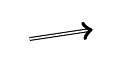
\begin{tikzpicture}\draw[->,double] (0,0)--(0.8,0.12);\end{tikzpicture}}}

\uline{Scholie} Par les bijections (34) (38), on transporte sur
$\unsure{g}_{\rho,\sigma},\ S_0g_{\rho,\sigma}$ les structures de groupes
naturelles de $\unsure{\widetilde{\Gamma}_{\rho,\sigma}},\
\unsure{\Gamma^{b_0}_{\rho,\sigma}}$.
Explicitant cette structure de groupe on trouve notamment pour $Sg_{\rho,\sigma}$
\[
\tag{\unsure{39|37}}
\left\{\begin{gathered}
(\alpha',\beta')(\alpha,\beta)=\alpha''\beta'',\quad
\text{avec }\alpha''=u'(\alpha)\alpha',\quad\beta''=u'(\beta)\beta'.\\
u'=u_{\unsure{\zeta|\xi}',\eta'}:\
\diagram{\begin{tikzcd}[column sep=large]
\unsure{\mathcal{C}}\arrow[r] & \unsure{\mathcal{C}}
\end{tikzcd}},\quad\text{défini par }
\left\{\begin{aligned}
u(\rho)&=\unsure{\zeta|\xi}\rho=\operatorname{int}(\alpha)\rho\\
u(\sigma)&=\eta\sigma=\operatorname{int}(\beta)\sigma
\end{aligned}\right.
\end{gathered}\right.
\]
(avec $\unsure{\zeta|\xi}=\alpha\rho(\alpha)^{-1},\ \eta=\beta\sigma(\beta)^{-1}$).

Dans $\unsure{S_0\Gamma^{b_0}_{\rho,\sigma}}$ on a un sous-groupe isom. à $L_0$, i.e.
\margin{\inserted{
\[
\tag{39}
\diagram{\begin{tikzcd}[column sep=large,row sep=small]
L_0\arrow[r] & \unsure{S\Gamma'_{\rho,\sigma}}\\
\unsure{\ell}\arrow[r,mapsto] & (\ell,1,1)
\end{tikzcd}}
\]
et on a suite exacte
\[
\tag{40}
\diagram{\begin{tikzcd}[column sep=small]
1\arrow[r] & L_0\arrow[r] & \unsure{S\Gamma'_{\rho,\sigma}}\arrow[r]
 & \unsure{\Gamma}_{\rho,\sigma}\arrow[r] & 1
\end{tikzcd}}
\]
}}

\deleted{
$\bullet$ \unsure{Posons maintenant}
\[
\tag{39}
\begin{gathered}
M_{\rho,\sigma}\subset\operatorname{Aut}(\unsure{\mathcal{C}})\\
\Vert\;\mathrm{dfn}\\
\left\{u\ \middle|\
\begin{array}{l}
\text{\unsure{a)|1°)} }u\ \deleted{\unsure{qui}}\ \text{fixe les classes de conj. de }\rho,\sigma\text{ dans }\unsure{\mathcal{C}},\\
\quad\text{i.e. }\exists\alpha_0,\beta_0\in\unsure{\mathcal{C}}\ \deleted{\unsure{\text{tels que}}}\ \text{avec }\
u(\rho)=\operatorname{int}(\alpha_0)\rho,\quad u(\sigma)=\operatorname{int}(\beta_0)\sigma,\\
\text{\unsure{b)|2°)} }u\ \text{fixe la classe de conjugaison de }L_0,\\
\quad\text{i.e. }\exists f\in\unsure{\mathcal{C}}\ \text{tel que }u(L_0)=\operatorname{int}(f^{-1}).L_0,\\
\quad\text{i.e. }fu\in\operatorname{Norm}_{\operatorname{Aut}(\unsure{\mathcal{C}})}(L_0)
\end{array}\right\}
\end{gathered}
\]
donc par définition de
\[
\tag{41}
\unsure{\mathcal{T}|\Gamma}_{\rho,\sigma}\overset{\mathrm{dfn}}{=}
Z_\rho\mathbin{\times}_{\Gamma_{\rho,\sigma}}Z_\sigma
\]
donc
\[
\tag{42}
\diagram{\begin{tikzcd}[column sep=small]
1\arrow[r] & SZ_\rho\times SZ_\sigma\arrow[r]
 & \unsure{\mathcal{T}|\Gamma}_{\rho,\sigma}\arrow[r,"\unsure{\delta_{\mathcal{T}}}"]
 & \Gamma_{\rho,\sigma}\arrow[r] & 1
\end{tikzcd}}
\]
}
\mspage{509}
% ===== LM_C3-511-529: second pass, checked against the scans =====
\scanpage{511}
\mspage{558}

\[
\diagram{\begin{tikzcd}[ampersand replacement=\&,column sep=large]
L_0 \arrow[r] \& S\deleted{\unsure{\mathcal{T}}}\Gamma_{\rho,\sigma}^{0}\subset B_{\rho,\sigma}\times Z_\rho\times Z_\sigma \\
\ell \arrow[r,mapsto] \& (\ell,1,1)
\end{tikzcd}}\tag{40}
\]
et l'action de $L_0$ par translation à g. sur
$\unsure{S\mathcal{T}'_{\rho,\sigma}|S\Gamma'_{\rho,\sigma}}$
devient, par $(39)$, l'action sur $S\unsure{\mathscr{G}|\mathcal{G}}_{\rho,\sigma}$ donnée par
\[
(\alpha,\beta)\longmapsto(\ell\alpha,\ell\beta).\tag{41}
\]

Posons donc
\margin{\unsure{noté} $\unsure{\Gamma|\mathcal{T}}_{\rho,\sigma}^{0}$ ds \S\,48, $\overline{\text{\uline{IX}}}$ $\unsure{\#}$.}
\[
\deleted{\unsure{\mathcal{T}}}\Gamma_{\rho,\sigma}^{0}
\overset{\mathrm{dfn}}{=}
S\deleted{\unsure{\mathcal{T}}}\Gamma_{\rho,\sigma}^{0}/\operatorname{Im}L_0
\simeq Z_\rho\mathbin{\times}_{\gamma_{\rho,\sigma}}Z_\sigma,
\tag{42}
\]
on trouve que $(39)$ induit une bijection canonique
\[
\diagram{\begin{tikzcd}[ampersand replacement=\&,column sep=large]
\deleted{\unsure{\mathcal{T}}}\Gamma_{\rho,\sigma}^{0}\arrow[r,"\sim"]\&L_0\backslash S\unsure{\mathscr{G}|\mathcal{G}}_{\rho,\sigma}
\end{tikzcd}}
\deleted{\unsure{\simeq Z_\rho\times Z_\sigma}}
\tag{43}
\]
\deleted{L'expression $(37)$ de $S_0\mathcal{T}_{\rho,\sigma}$ donne une suite \inserted{exacte},}
\[
\deleted{(44)\quad 1\longrightarrow L_0\times S}
\qquad\deleted{\text{Notons les suites}}
\]
Posant
\[
\left\{\begin{aligned}
\underset{\cdot}{S}Z_\rho&\overset{\mathrm{dfn}}{=}\operatorname{Ker}(Z_\rho\longrightarrow\Gamma_{\rho,\sigma})=\operatorname{Centr}_{\unsure{\mathcal{G}}}(\rho)\\
SZ_{\rho}&=\operatorname{Ker}(Z_{\rho}\mathbin{-}\Gamma_{\rho,\unsure{2|\sigma}})=\operatorname{Centr}_{\mathcal{G}}(\sigma)
\end{aligned}\right.\tag{44}
\]
\margin{introduire aussi
$S\Gamma_{\rho,\sigma}=\operatorname{Ker}(\Gamma_{\rho,\sigma}\longrightarrow\gamma_{\rho,\sigma}),$
$SG_{\rho,\sigma}=\operatorname{Ker}(G_{\rho,\sigma}\longrightarrow\gamma_{\rho,\sigma})=\mathcal{G}_{\rho,\sigma}=\mathcal{G}$.}

on a donc des suites exactes
\[
\left\{\begin{gathered}
\diagram{\begin{tikzcd}[ampersand replacement=\&,column sep=small]
1\arrow[r,no head]\&SZ_\rho\arrow[r]\&Z_\rho\arrow[r,no head]\&\Gamma_{\unsure{\rho\sigma|\rho,\sigma}}\arrow[r,no head]\&1
\end{tikzcd}}\\
\diagram{\begin{tikzcd}[ampersand replacement=\&,column sep=small]
1\arrow[r,no head]\&SZ_\sigma\arrow[r,no head]\&Z_\sigma\arrow[r,no head]\&\Gamma_{\rho,\sigma}\arrow[r,no head]\&1
\end{tikzcd}}
\end{gathered}\right.\,,\tag{45}
\]
et les expressions $(37)$, $(42)$ de $S\deleted{\unsure{\mathcal{T}}}\Gamma_{\rho,\sigma}^{0}$, $\deleted{\unsure{\mathcal{T}}}\Gamma_{\rho,\sigma}^{0}$ donnent
\[
\diagram{\begin{tikzcd}[ampersand replacement=\&,column sep=small]
1\arrow[r]\&L_0\times SZ_\rho\times SZ_\sigma\arrow[r,no head]\&S_0\deleted{\unsure{\mathcal{T}}}\Gamma_{\rho,\sigma}^{0}\arrow[r,no head]\&\gamma_{\rho,\sigma}\arrow[r,no head]\&1
\end{tikzcd}}\tag{46}
\]
\[
\diagram{\begin{tikzcd}[ampersand replacement=\&,column sep=small]
1\arrow[r]\&SZ_\rho\times SZ_\sigma\arrow[r]\&\deleted{\unsure{S}}\deleted{\unsure{\mathcal{T}}}\Gamma_{\rho,\sigma}^{0}\arrow[r,no head]\&\gamma_{\rho,\sigma}\arrow[r]\&1
\end{tikzcd}}.\tag{47}
\]
\uline{NB} Dans le cas $\mathcal{G}=\mathrm{Sl}(2,\widehat{\mathbb{Z}})$, $\rho$ et $\sigma$ ``modulaires'', on retrouve \deleted{\illegible{1}} les $S_0\deleted{\unsure{\mathcal{T}}}\Gamma_{\rho,\sigma}^{0\unsure{4|\#}}$ et $\deleted{\unsure{\mathcal{T}}}\Gamma_{\rho,\sigma}^{0}$ de \S\,48 $\overline{\text{IX}}$.

\mspage{510}
\scanpage{512}
\mspage{559}

Soit maintenant
\[
\begin{gathered}
S_0M_{\rho,\sigma}^{0*}\subset
S\deleted{\unsure{\mathcal{T}}}\Gamma_{\rho,\sigma}^{0}\times G_{\rho,\sigma}
\quad(\subset B_{\rho,\sigma}\times Z_\rho\times Z_\sigma\times G_{\rho,\sigma})\\
\overset{\mathrm{dfn}}{=}\\
\left\{(u,a,b,U)\,\middle|\,
\underbrace{\delta_B(u)=\delta_\rho(a)=\delta_\sigma(b)=\delta_G(U)}_{\text{relation dans }\gamma_{\rho,\sigma}\ \text{cf }(17)}\right\}
\end{gathered}\tag{49}
\]
\[
\begin{gathered}
M_{\rho,\sigma}^{0}\subset T_\rho\times T_\sigma\times G_{\rho,\sigma}\\
\overset{\mathrm{dfn}}{=}\\
\left\{(a,b,U)\,\middle|\,
\underbrace{\delta_\rho(a)=\delta_\sigma(b)=\delta_G(U)}_{\text{relations dans }\gamma_{\rho,\sigma}}\right\}
\end{gathered}\tag{50}
\]
On a donc un hom canonique
\[
\diagram{\begin{tikzcd}[ampersand replacement=\&,column sep=large]
SM_{\rho,\sigma}^{0}\arrow[r]\&M_{\rho,\sigma}^{0}\\
(u,a,b,U)\arrow[r]\&\deleted{\unsure{(u}}(a,b,U)
\end{tikzcd}}\tag{51}
\]
dont le noyau est formé des $(u,1,1,1)$ où $u\in B_{\rho,\sigma}$ tel que $\delta_B(u)=1$ i.e. $u\in L_0$, d'où une suite exacte
\[
\diagram{\begin{tikzcd}[ampersand replacement=\&,column sep=small]
1\arrow[r,no head]\&L_0\arrow[r]\&SM_{\rho,\sigma}^{0}\arrow[r]\&M_{\rho,\sigma}^{0}\arrow[r,no head]\&1
\end{tikzcd}}\tag{52}
\]
et des hom canoniques
\[
\diagram{\begin{tikzcd}[ampersand replacement=\&,column sep=large,row sep=small]
\&G_{\rho,\sigma}\\
M_{\rho,\sigma}^{0}\arrow[ur,"\Theta_G"]\arrow[r,"\Theta_\rho",very thick]\arrow[dr,"\Theta_\sigma"']\&Z_\rho\\
\&Z_\sigma
\end{tikzcd}}\tag{53}
\]
\[
\left(\text{resp.}\quad
\diagram{\begin{tikzcd}[ampersand replacement=\&,column sep=small,row sep=small]
\&U\\
(a,b,U)\arrow[ur,mapsto]\arrow[r,mapsto]\arrow[dr,mapsto]\&a\\
\&b
\end{tikzcd}}\right),
\]
\unsure{redonnant} les hom analogues sur $SM_{\rho,\sigma}^{0}$ par composition avec $(41)$, et de plus on a un hom canonique
\[
\diagram{\begin{tikzcd}[ampersand replacement=\&,column sep=large]
SM_{\rho,\sigma}^{0}\arrow[r,"\Theta_B"]\&B_{\rho,\sigma}\\
(u,a,b,U)\arrow[r,mapsto]\&u
\end{tikzcd}}.\tag{54}
\]

\mspage{511}
\scanpage{513}

On a aussi \deleted{\unsure{de}} l'interprétation
\[
S_0M_{\rho,\sigma}^{0}\simeq M_{\rho,\sigma}^{0}\mathbin{\times}_{\gamma_{\rho,\sigma}}B_{\rho,\sigma};\tag{55}
\]
( $S_0M_{\rho,\sigma}^{0}$ s'exprime à l'aide de $M_{\rho,\sigma}^{0}$ et $B_{\rho,\sigma}$, et on \unsure{voit} que l'extension de $M_{\rho,\sigma}$ par $L_0$ est l'image inverse de l'extension $B_{\rho,\sigma}$ de $\gamma_{\rho,\sigma}$ par $L_0$. Et on a
\[
M_{\rho,\sigma}^{0}\simeq
\underbrace{Z_\rho\mathbin{\times}_{\gamma_{\rho,\sigma}}Z_\sigma}_{\deleted{\unsure{\mathcal{T}}}\Gamma_{\rho,\sigma}^{0}}
\mathbin{\times}_{\gamma_{\rho,\sigma}}G_{\rho,\sigma}.\tag{56}
\]
d'où on déduit (comme $\delta_\rho,\delta_\sigma,\delta_G$ sont épi)
\[
\diagram{\begin{tikzcd}[ampersand replacement=\&,column sep=small]
1\arrow[r,very thick]\&\deleted{\unsure{\Gamma_\rho|T_\rho}}\underbrace{SZ_\rho\times SZ_\sigma\times\unsure{\mathcal{G}}}_{\overset{\mathrm{dfn}}{=}M_{\rho,\sigma}^{0+}}\arrow[r]\&\unsure{M_{\rho,\sigma}'|M_{\rho,\sigma}^{0}}\arrow[r,"\delta_M^{\unsure{\#|*}}"]\&\gamma_{\rho,\sigma}\arrow[r]\&1
\end{tikzcd}}\tag{57}
\]
où on a \deleted{\unsure{posé}} $(44)$
\[
\deleted{(\unsure{48|58})}\qquad
\left\{\begin{aligned}
SZ_\rho&=Z_\rho\cap\mathcal{G}={\underset{\deleted{\unsure{\mathrm{aut}}}}{\uline{\operatorname{Centr}}}}_{\mathcal{G}}(\rho)\\
SZ_\sigma&=Z_\sigma\cap\mathcal{G}={\underset{\deleted{\unsure{\mathrm{aut}}}}{\uline{\operatorname{Centr}}}}_{\mathcal{G}}(\sigma)
\end{aligned}\right.
\]
De même on a
\[
S_0M_{\rho,\sigma}^{0}\simeq
\underbrace{B_{\rho,\sigma}\mathbin{\times}_{\gamma_{\rho,\sigma}}Z_\rho\mathbin{\times}_{\gamma_{\rho,\sigma}}Z_\sigma}_{S_0\deleted{\unsure{\mathcal{T}}}\Gamma_{\rho,\sigma}^{0}}
\mathbin{\times}_{\gamma_{\rho,\sigma}}G_{\rho,\sigma}
\tag{49}
\]
d'où on a une suite exacte canonique
\[
\diagram{\begin{tikzcd}[ampersand replacement=\&,column sep=small]
1\arrow[r]\&L_0\times SZ_\rho\times SZ_\sigma\times\mathcal{G}\arrow[r]\&S_0M_{\rho,\sigma}^{0}\arrow[r]\&\Gamma_{\rho,\sigma}\arrow[r,no head]\&1
\end{tikzcd}}\tag{50}
\]
Considérons l'hom. can
\[
\diagram{\begin{tikzcd}[ampersand replacement=\&,column sep=large]
\mathcal{G}\arrow[r,"i_{\mathcal{G}}"]\&M_{\rho,\sigma}^{0}\\
U\arrow[r,mapsto]\&(1,1,U)
\end{tikzcd}},\tag{51}
\]

\mspage{512}
\scanpage{514}
\mspage{560}

son image est le troisième facteur dans le noyau de $(57)$, et on a une suite exacte canonique (déduite de $(56)$--$(57)$)
\[
\diagram{\begin{tikzcd}[ampersand replacement=\&,column sep=small]
1\arrow[r]\&\underset{\inserted{\substack{\text{parfois noté}\\\mathcal{G}_{\rho,\sigma}?}}}{\unsure{\mathcal{G}}}\arrow[r]\&M_{\rho,\sigma}^{0}\arrow[r]\&\deleted{\unsure{\mathcal{T}}}\Gamma_{\rho,\sigma}^{0}\arrow[r,no head]\&1
\end{tikzcd}}\tag{52}
\]
\margin{$(53')$ \diagram{\begin{tikzcd}[ampersand replacement=\&,column sep=small]
1\arrow[r]\&SZ_\rho\times SZ_\sigma\arrow[r]\&M_{\rho,\sigma}^{0}\arrow[r]\&\unsure{G|G_1}\arrow[r,no head]\&1
\end{tikzcd}}}
et de même on a (via $(49)$ ou $50)$)
\[
\left\{\begin{aligned}
&(53)\quad\diagram{\begin{tikzcd}[ampersand replacement=\&,column sep=small]
1\arrow[r]\&\mathcal{G}\arrow[r]\&S_0M_{\rho,\sigma}^{0}\arrow[r]\&S_0\deleted{\unsure{\mathcal{T}}}\Gamma_{\rho,\sigma}^{0}\arrow[r]\&1
\end{tikzcd}}.\\[1ex]
&\text{Considérons l'application}\\[1ex]
&(54)\quad\diagram{\begin{tikzcd}[ampersand replacement=\&,column sep=large]
S_0M_{\rho,\sigma}^{0}\arrow[r]\&\mathcal{G}\times\mathcal{G}\times\mathcal{G}\\
\{u,a,b,U\}\arrow[r,mapsto]\&(ua^{-1},ub^{-1},uU^{-1})=(\alpha,\beta,f)
\end{tikzcd}}
\end{aligned}\right.
\]
on \unsure{voit} \deleted{\illegible{1}} par le corollaire p.\,557 (cf $(37)$) que cela induit une bijection
\[
S_0M_{\rho,\sigma}^{0}\simeq(S\unsure{\mathscr{G}|\mathcal{G}}_{\rho,\sigma})\times\mathcal{G}.
\tag{55}
\]
On a ainsi, pour un $x\in S_0M_{\rho,\sigma}^{0}$, d'une part les quantités
\[
\diagram{\begin{array}{cccc}
u,&a,&b,&U\\
\rotatebox{90}{$\in$}&\rotatebox{90}{$\in$}&\rotatebox{90}{$\in$}&\rotatebox{90}{$\in$}\\
B_{\rho,\sigma}&Z_\rho&Z_\sigma&G_{\rho,\sigma}
\end{array}},\tag{56}
\]
associés, d'autre part les éléments
\[
\alpha,\beta,f,\quad\unsure{\zeta|\xi},\eta,\quad\alpha_0\ \beta_0,g,h
\qquad\text{tous }\in\mathcal{G}\tag{57}
\]
\inserted{où $(\alpha,\beta,f)$} définis en termes de $(56)$ dans $(54)$, et où on a posé
\[
\left\{\begin{aligned}
\zeta&=\alpha\rho(\alpha)^{-1},\quad
\eta=\beta\sigma(\beta)^{-1},\quad
\alpha_0=f^{-1}\alpha\unsure{\#|\zeta},\quad\beta_0=f^{-1}\beta,\\
g&=\alpha_0\rho(\alpha_0)^{-1}=f^{-1}\zeta\rho(f),\quad
h=\beta_0\sigma(\beta_0)^{-1}=f^{-1}\eta\sigma(f)
\end{aligned}\right.\tag{58}
\]

\mspage{513}
\scanpage{515}

On aura, en termes de $\alpha,\beta,f$, les expressions suivantes de l'action de $U$ sur $\mathcal{G}$ :
\[
\left\{\begin{aligned}
U(\rho)&=\operatorname{int}(f^{-1}\alpha)\deleted{\unsure{\operatorname{int}(\alpha)}}\rho
 =\operatorname{int}(f^{-1})(\zeta\rho)\\
U(\sigma)&=\operatorname{int}(f^{-1}\beta)\deleted{\unsure{\operatorname{int}(\beta)}}(\sigma)
 =\operatorname{int}(f^{-1})(\eta\sigma).
\end{aligned}\right.\tag{59}
\]
\deleted{\unsure{et}\ $\unsure{\zeta|\xi},\unsure{\eta}$\unsure{.}}

\uline{\unsure{Remarque|Remarq.}} Finalement, dans tous ces développements, on n'a pas vraiment utilisé la soi-disante ``hyp. fondamentale'' $(20)\deleted{\unsure{b}}$, \deleted{\unsure{et}} sauf la partie a). En l'absence de b), il y a lieu d'introduire
\[
\begin{gathered}
\Sigma_{\rho,\sigma}^{\mathrm{eff}}\subset\Sigma_{\rho,\sigma}\subset\mathcal{G}\times\mathcal{G}\\[-1pt]
\begin{array}{c@{\qquad}l}
\rotatebox{90}{$=$}&\\[-3pt]
\multicolumn{2}{l}{\left\{(\zeta,\eta)\in\unsure{\mathcal{G}|\Sigma_\rho}\times\mathcal{G}\mid
\exists u\in B_{\rho,\sigma},\ u(\rho)=\zeta\rho,\ u(\sigma)=\eta\sigma\right\},}
\end{array}
\end{gathered}\tag{60}
\]
qui n'est donc autre que l'image de l'application $(9)$ : couples \uline{effectifs} $(\zeta,\eta)$ satisfaisant les conditions définissant \deleted{\unsure{les}\ $\unsure{(5)}$}\inserted{$\Sigma_{\rho,\sigma}$ (cf $(8)$)}\unsure{)}

\deleted{L'application
$\diagram{\begin{tikzcd}[ampersand replacement=\&,column sep=large]
S\unsure{\mathscr{G}|\mathcal{G}}_{\rho,\sigma}\arrow[r]\&\Sigma_{\rho,\sigma}
\end{tikzcd}}$
\inserted{$(28)$} (ne sera pas néc. surjective, son image \unsure{est|sera} $\Sigma_{\rho,\sigma}^{\mathrm{eff}}\inserted{\simeq B_{\rho,\sigma}}$), d'ailleurs il n'y a rien à changer.}
\margin{\unsure{puis|par}\par\unsure{bij.|bis}}

notons
\[
\begin{aligned}
S\unsure{\mathscr{G}|\mathcal{G}}_{\rho,\sigma}^{\mathrm{eff}}
 &=\text{Image inverse de }\Sigma_{\rho,\sigma}^{\mathrm{eff}}\\
 &\text{par }\diagram{\begin{tikzcd}[ampersand replacement=\&,column sep=large]
S\unsure{\mathscr{G}|\mathcal{G}}_{\rho,\sigma}\arrow[r,no head]\&\Sigma_{\rho,\sigma}
\end{tikzcd}}\quad(28),
\end{aligned}\tag{61}
\]
\deleted{l'image inverse}
et c'est sur $S\unsure{\mathscr{G}|\mathcal{G}}_{\rho,\sigma}^{\mathrm{eff}}$ qu'on aura une structure

\mspage{514}
\scanpage{516}
\mspage{561}

de groupe \unsure{isomorphe} \unsure{à|:} $S_0\mathcal{T}_{\rho,\sigma}^{0}$, par l'isomorphisme (qui remplace (38))
\diagram{\begin{tikzcd}[ampersand replacement=\&,column sep=large]
 S_0\deleted{\unsure{\mathcal{T}}}\Gamma_{\rho,\sigma}^{0} \arrow[r,phantom,"\simeq"] \& S_0\unsure{\mathscr{G}|\mathcal{G}}_{\rho,\sigma}^{\mathrm{eff}}\,. \\
 (\underline{u},\underline{a},\underline{b}) \arrow[r] \& (\underbrace{ua^{-1}}_{\zeta},\underbrace{ub^{-1}}_{\eta})
\end{tikzcd}\quad(62)}

Ceci posé, revenons à $M_{\rho,\sigma}^{\sim}$, et la suite exacte
\diagram{\begin{tikzcd}[ampersand replacement=\&,column sep=small]
 1 \arrow[r] \& \mathcal{G}_{0,3}^{+\wedge} \arrow[r] \& M_{\unsure{0,3|\rho,\sigma}}^{\sim} \arrow[r] \& \underbrace{\Gamma_{0,3}^{\sim}}_{\Gamma_{\mathbb Q}^{\sim}} \arrow[r] \& 1
\end{tikzcd}\quad(63).}

Considérons le sous-groupe
\[
\begin{aligned}
(64)\qquad
\Gamma_{\mathbb Q}^{\prime\sim}
 &= \operatorname{Ker}\bigl(\Gamma_{0,3}^{\sim}
 \xrightarrow{(\varepsilon_3,\deleted{\unsure{\varepsilon_2}})}
 \{\pm1\}\deleted{\unsure{\times\{\pm1\}}}\bigr)\\
 &= \{\gamma\in\Gamma_{0,3}^{\sim}\mid\mu(\gamma)\equiv1\ (\unsure{3}\deleted{\unsure{12}})\}.
\end{aligned}
\]
\deleted{\illegible{3}}
\deleted{\unsure{deux facteurs}}

et soit \deleted{$\unsure{M_{0,3}^{\prime\sim}}$}
\[
 (65)\qquad M_{0,3}^{\prime\sim}
 = \text{\unsure{Image inv.} de }\Gamma_{0,3}^{\prime\sim}\text{ dans }M_{0,3}^{\sim}.
\]

Soit $\mathcal{G}$ un groupe profini, et
\[
 (66)\qquad\psi:\mathcal{G}_{0,3}^{+\wedge}\longrightarrow\mathcal{G},
\]
un hom. \inserted{continu} surjectif --- ce qui revient au $\overline{\mathrm m}$ que de se donner deux éléments
\[
 (67)\qquad\rho_{\mathcal{G}},\unsure{\sigma_{\mathcal{G}}}\in\mathcal{G}
\]
(les images de $\rho,\sigma$ par $\psi$) satisfaisant
\[
 (68)\qquad\rho_{\mathcal{G}}^3=\sigma_{\mathcal{G}}^2=1.
\]
\mspage{515}
\scanpage{517}

\margin{l'introduire par conditions équivalentes :

\unsure{a)}
\diagram{\begin{tikzcd}[ampersand replacement=\&,column sep=large]
 M_{0,3}^{\prime\sim}[0] \arrow[r] \& \Sigma_{\rho,\sigma}^{\text{\textcircled{eff}}}
\end{tikzcd}} \unsure{tout}

b) $\forall u\in M_{0,3}^{\prime\sim},\ \exists u_{\unsure{\mathcal{G}}}\in\operatorname{Aut}\mathcal{G}$ tel que
$u_{\unsure{M|\mathcal{G}}}\circ\psi=\psi\circ u$

b') Idem avec $u\in M_{0,3}^{\prime\sim}[0]$

\unsure{c)} $\exists\psi_M$ qui prolonge $\psi$

c') $\exists\psi_G$ qui prolonge $\psi$

On dira donc que \deleted{\unsure{eff.}} \unsure{automatique|autom.}

$\psi$ est \uline{\unsure{effectif}} si (20) b) satisfait}

\uline{Définition} On dira que $\psi$ est \uline{effectif} si pour tout
$u\in M_{0,3}^{\prime\sim}[0]$, posant $u(\rho)=\zeta\rho$, $u(\sigma)=\eta\sigma$,
\[
 (\zeta_{\mathcal{G}},\eta_{\mathcal{G}})
 =(u(\zeta),u(\eta))\in\Sigma_{\rho,\sigma}
\]
effectif (i.e. $\in\Sigma_{\rho,\sigma}^{\mathrm{eff}}$, i.e. $\exists u_{\mathcal{G}}$ \unsure{autom.} $\mathcal{G}$ tel qu'on ait \deleted{$\unsure{u_{\mathcal{G}}\rho}$}
\[
 (69)\qquad
 u_{\mathcal{G}}(\rho_{\mathcal{G}})=\zeta_{\mathcal{G}}\rho_{\mathcal{G}},
 \qquad
 u_{\mathcal{G}}(\sigma_{\mathcal{G}})=\eta_{\mathcal{G}}\sigma_{\mathcal{G}}
\]
ou, ce qui revient au $\overline{\mathrm m}$, qu'on a commutativité dans
\diagram{\begin{tikzcd}[ampersand replacement=\&,column sep=large,row sep=large]
 \mathcal{G}_{0,3}^{+\wedge} \arrow[r,"u"] \arrow[d,"\psi"'] \& \mathcal{G}_{0,3}^{+\wedge} \arrow[d,"\psi"] \\
 \mathcal{G} \arrow[r,"u_{\mathcal{G}}"'] \& \mathcal{G}
\end{tikzcd}\quad(70).}

(Donc dire que c'est le cas pour \unsure{tt} $u\in M_{0,3}^{\prime\sim}\deleted{[0]}$ signifie que ces $u$ transforment $\operatorname{Ker}\psi$ en lui $\overline{\mathrm m}$ --- ou aussi, que
$M_{0,3}^{\prime\sim}\deleted{\unsure{[0]}}$
$(=M_{0,3}^{\prime\sim}[0].\mathcal{G}_{0,3}^{+\wedge})$ tout entier stabilise $\operatorname{Ker}\psi$.
\deleted{Quand} Cette condition est donc automatiquement remplie quand $\mathcal{G},\rho_{\mathcal{G}},\sigma_{\mathcal{G}}$ satisfont \unsure{la condition|les conditions} b) de (20).

On a fait ce qu'il fallait pour avoir \unsure{le}
\mspage{516}
\scanpage{518}
\mspage{562}

\uline{Théorème} Soit $\psi=\psi_{\mathcal{G}}:\mathcal{G}_{0,3}^{+\wedge}\longrightarrow\mathcal{G}$ un hom surjectif effectif (cf ci-dessus).
Alors il existe un hom unique
\[
 (71)\qquad\psi_M:\deleted{\unsure{S_0}}M_{0,3}^{\prime\sim\deleted{\unsure{*}}}
 \longrightarrow\deleted{\unsure{S_0}}M_{\rho_{\mathcal{G}},\sigma_{\mathcal{G}}}^{0}
\]
\deleted{rendant commutatif le diagramme}
\diagram{\deleted{\begin{tikzcd}[ampersand replacement=\&,column sep=large,row sep=large]
 \mathcal{G}_{0,3}^{+\wedge} \arrow[r,"\unsure{\psi|\varphi}"] \arrow[d,"\psi"'] \& \deleted{\unsure{\mathcal{G}}}\,M_{0,3}^{\prime\sim} \arrow[d,"\psi"] \\
 \deleted{\unsure{\mathcal{G}}}\,\mathcal{G} \arrow[r] \& M_{\rho_{\mathcal{G}},\sigma_{\mathcal{G}}}^{0}\ (\overset{\mathrm{dfn}}{=}M_{\psi}^{0})
\end{tikzcd}\quad(72)}}

\margin{En fait, on a \unsure{bien sûr en} premier lieu un hom
\diagram{\begin{tikzcd}[ampersand replacement=\&,column sep=large]
 S_0M_{0,3}^{\prime\sim} \arrow[r] \& S_0M_{\psi}^{0}.
\end{tikzcd}}}

ayant la propriété suivante : si \deleted{$\unsure{u\in}$}
$u\unsure{=|\in}M_{0,3}^{\prime\sim}$ est de la forme $u_{\alpha,\beta,f}$
($\alpha,\beta,f\in\mathcal{G}_{0,3}^{+\wedge}$, satisfaisant l'équation des lacets
$\alpha\rho(\alpha)^{-1}=\beta\sigma(\beta)^{-1}\ell_1^{\nu}$), alors
$\psi_M(u)$ est l'élément de \deleted{$\unsure{M_{\rho_{\mathcal{G}},\sigma_{\mathcal{G}}}^{0}}$} $M_{\psi}^{0}$ défini par les invariants $\psi(\alpha),\psi(\beta);\psi(f)$.

\uline{Corollaire} On a alors des hom de suites exactes
\diagram{\begin{tikzcd}[ampersand replacement=\&,column sep=small,row sep=large]
 1 \arrow[r] \& \mathcal{G}_{0,3}^{+\wedge} \arrow[r,no head] \arrow[d,"\psi_{\mathcal{G}}"'] \& M_{0,3}^{\prime\sim} \arrow[r] \arrow[d,"\psi_M"] \& \Gamma_{\mathbb Q}^{\prime\sim} \arrow[r] \arrow[d,"\unsure{\psi_{\mathcal{T}}|\psi_{\Gamma}}"] \& 1 \\
 1 \arrow[r] \& \mathcal{G} \arrow[r] \& M_{\psi}^{0} \arrow[r] \& \deleted{\unsure{\mathcal{T}}}\Gamma_{\psi}^{0} \arrow[r] \& 1
\end{tikzcd}\quad(72).}

(L'hom. $\psi_M$ s'explicite à l'aide de trois homomorphismes
\mspage{517}
\scanpage{519}

\[
\left\{\begin{aligned}
\psi_{T_\rho}&:\Gamma_{\mathbb Q}^{\prime\sim}\longrightarrow \unsure{Z_\rho|T_\rho}\\
\psi_{T_\sigma}&:\Gamma_{\mathbb Q}^{\sim}\longrightarrow \unsure{Z_\sigma|T_\sigma}
\end{aligned}\right.\qquad(73)
\]
\[
\psi_G:M_{0,3}^{\prime\sim}\longrightarrow G_{\rho,\sigma}\qquad(74)
\]
\margin{NB on écrit pour simplifier $\rho,\sigma$ au lieu de $\rho_{\mathcal G},\sigma_{\mathcal G}$ en indices}

\deleted{satisfaisant les conditions}
(Pour \deleted{$\unsure{u}$} $x\in M_{0,3}^{\prime\sim}$,
\inserted{$\dot x$ son image dans $\Gamma_{\mathbb Q}^{\prime\sim}$,}
\deleted{$a=\psi_{\unsure{T_\rho|\Gamma_\rho}}(\dot x),\ b=\psi_{\unsure{T_\rho|\Gamma_\rho}}(\unsure{y|\dot x}),\ U=\unsure{\psi u|\psi(x)}$}
\[
\deleted{\unsure{\delta_G(}}\quad
 a=\psi_{\unsure{T_\rho|\Gamma_\rho}}(\dot x),\quad b=\psi_{\unsure{T_\sigma|\Gamma_\sigma}}(\dot x),\quad U=\psi_G(x),
\qquad(75)
\]
on a
\[
\delta_\rho(a)=\delta_\sigma(b)=\delta_G(U)\quad\text{dans }\gamma_{\rho,\sigma}\qquad(76)
\]
i.e. les trois hom composés
\diagram{\begin{tikzcd}[ampersand replacement=\&,column sep=large,row sep=large]
\&\Gamma_{\mathbb Q}^{\prime\sim}\arrow[r,"\psi_{T_\rho}"]\&T_\rho\arrow[rd,"\delta_\rho"]\&\\
M_{0,3}^{\prime\sim}\arrow[ru,"\mathrm{can}"]\arrow[r,"\mathrm{can}"]\arrow[rrd,"\psi_G"',"\unsure{1}"{pos=.43}]\arrow[rrd,shorten >=55pt,shorten <=40pt]\&\Gamma_{\mathbb Q}^{\prime\sim}\arrow[r,no head,"\psi_{T_\sigma}"]\&T_\sigma\arrow[r,"\delta_\sigma"]\&\gamma_{\rho,\sigma}\arrow[ld,"\delta_G"]\\
\&\&G_{\rho,\sigma}\&
\end{tikzcd}\qquad(77)}
sont égaux. De plus, on aura d'après (71),
\[
\psi_G|\mathcal G_{0,3}^{+\wedge}=\psi_{\mathcal G},\qquad(78)
\]
et enfin ceci :

(79) Si $x\in \deleted{\unsure{M}}M_{0,3}^{\prime\sim}$, $U=\psi_G(x)$, on a commutativité dans
\diagram{\begin{tikzcd}[ampersand replacement=\&,column sep=huge,row sep=large]
\mathcal G_{0,3}^{+\wedge}\arrow[r,"\psi"]\arrow[d,"\operatorname{int}(x)|\mathcal G_{0,3}^{+\wedge}"']\&\mathcal G\arrow[d,"\operatorname{int}(U)|\mathcal G"]\\
\mathcal G_{0,3}^{+\wedge}\arrow[r,"\psi"]\&\mathcal G
\end{tikzcd}\qquad(80)}

\hfill $.\ .\ .\ .\ .\ .$ 
\mspage{518}
\scanpage{520}
\mspage{563}

. On peut regarder tout ceci comme un énoncé de \uline{fonctorialité} des constructions faites, p.r. à un hom surjectif
\diagram{\begin{tikzcd}[ampersand replacement=\&]
\mathcal G\arrow[r,"\varphi=\varphi_{\mathcal G}"]\&\mathcal G'
\end{tikzcd}\qquad(81)}
\margin{\unsure{Il aurait} mieux valu prendre \unsure{donc}
\diagram{\begin{tikzcd}[ampersand replacement=\&]\mathcal G'\arrow[r,"\varphi"]\&\mathcal G\end{tikzcd}},
pour pouvoir spécialiser en $\mathcal G'$}
transformant le couple $(\rho,\sigma)$ de générateurs topologiques de $\mathcal G$ en un couple $(\rho',\sigma')$.
Il y a alors un unique homomorphisme
\diagram{\begin{tikzcd}[ampersand replacement=\&]
S_0M_{\mathcal G}^{0}\arrow[r,"\varphi_{M^0}"]\&S_0M_{\mathcal G'}^{0}
\end{tikzcd}\qquad(82)}
satisfaisant les conditions suivantes :

\margin{ceci montre que $\varphi_{SM}$ est déterminé quand on connaît les quatre hom $\varphi_B,\varphi_\rho,\varphi_\sigma,\varphi_G$}
a) $\unsure{\varphi_M|\varphi_{SM}}$ \unsure{passe} en quotient \unsure{en|à} des hom
\[
\left\{\begin{aligned}
\varphi_B&:B_{\rho,\sigma}\longrightarrow\unsure{Z_{\rho,\sigma}|\Sigma_{\rho,\sigma}}\\
\varphi_\rho&:Z_\rho\longrightarrow Z_{\rho'}\\
\varphi_\sigma&:Z_\sigma\mathrel{\relbar\joinrel\relbar} Z_{\sigma'}\\
\varphi_G&:G_{\rho,\sigma}\mathrel{\relbar\joinrel\relbar} G_{\rho',\sigma'}
\end{aligned}\right.\ ;\qquad(83)
\]

b) \deleted{On a commutativité dans le diagramme,}
\inserted{\deleted{Les hom $\varphi_B,\varphi_\rho,\varphi_\sigma$ \unsure{sont induits par}}}
\[
(84)\quad\left\{\begin{gathered}
\deleted{\text{\unsure{uniquement}}}\quad\varphi_G\qquad
\text{(ce qui montre que la connaissance}\\
\text{\illegible{1} de }\varphi_{SM}\ \unsure{b|se}\ \text{revient à celle de }\varphi_G\text{)};
\end{gathered}\right.
\]

c) On a commutativité dans
\diagram{\begin{tikzcd}[ampersand replacement=\&,column sep=large,row sep=large]
\mathcal G\arrow[r]\arrow[d,"\varphi=\varphi_{\mathcal G}"']\&G_{\rho,\sigma}\arrow[d,"\varphi_G"]\\
\mathcal G'\arrow[r]\&G_{\rho',\sigma'}
\end{tikzcd}\qquad(85)}
(ce qui montre, puisque $G_{\rho,\sigma}=B_{\rho,\sigma}\cdot\mathcal G$, que $\varphi_G$ est connu quand on connaît $\varphi_B$ ;

d) Pour $u\in B_{\rho,\sigma}$, \deleted{\unsure{désignant} par $u'$} \inserted{posant $u'=\varphi_B(u)$}, on a commutativité dans
\diagram{\begin{tikzcd}[ampersand replacement=\&,column sep=large,row sep=large]
\mathcal G\arrow[r,"u"]\arrow[d,"\varphi_{\mathcal G}"']\&\mathcal G\arrow[d,"\varphi_{\mathcal G}"]\\
\mathcal G'\arrow[r,"u'"]\&\mathcal G'
\end{tikzcd}\qquad(86)}
\mspage{519}
\scanpage{521}

-- (ce qui détermine $\varphi_B$ en termes de $\varphi=\varphi_{\mathcal G}$, donc \unsure{cela|elle} détermine $\unsure{\varphi_{S_0M}}$, et par passage au quotient, aussi
\[
 (87)\qquad \varphi_M:M_{\rho,\sigma}\longrightarrow M_{\rho',\sigma'}.
\]

Une autre façon, plus directe, de décrire $\varphi_{S_0M^0}$ ou $\varphi_M$, en termes des \deleted{coordonnées} \inserted{``paramètres''} $(\alpha,\beta,f)$ au lieu des $(u,a,b,U)$, est de dire qu'on \deleted{$\unsure{\varphi_{S_0M^0}}$ \unsure{transforme}} transforme un $u_{\alpha,\beta,f}$ en le $u_{\alpha',\beta',f'}$, où $\alpha',\beta',f'$ sont les images de $\alpha,\beta,f$ par $\varphi$:
\[
 (88)\qquad
 \varphi_{\deleted{\unsure{\mathcal G}}S_0\unsure{M_0|M^0}}
 \left(\underbrace{u_{\alpha,\beta,f}}_{\in\,S_0M^0_{\rho,\sigma}}\right)
 =u_{\alpha',\beta',f'},\quad
 \left\{\begin{aligned}
 \alpha'&=\varphi(\alpha),\\
 \beta'&=\varphi(\beta),\\
 f'&=\varphi(f).
 \end{aligned}\right.
\]

On retrouve, ainsi, sous une forme un peu plus précise, le \unsure{th.} précédent, en \deleted{\unsure{mettant}} l'appliquant au cas où $\mathcal G=\mathcal G_{0,3}^{+\wedge}$ (le ``cas universel'')$^*$, $\mathcal G'$ quelconque --- il \unsure{vaut} mieux dans la notation (81) interchanger le rôle de $\mathcal G$ et $\mathcal G'$.
\margin{$^*$ tout au moins ``universel'' p.r. à l'hyp. \unsure{suppl.} $\rho^3=1,\ \sigma^2=1$ dans $\mathcal G$.}
Il est bon d'\deleted{\unsure{expliciter}}\inserted{expliciter les invariants essentiels} (dans le cas ``universel'':

\deleted{pour}
\[
\begin{aligned}
 (90)\qquad
 \mathcal G'&=\mathcal G_{0,3}^{+\wedge},\qquad
 B_{\rho',\sigma'}^{\deleted{\unsure{0}}\,\prime}
 =M_{0,3}^{\prime\sim}[0],\qquad
 \gamma_{\rho',\sigma'}^{\unsure{\prime|0}}
 =\Gamma_{\mathbb Q}^{\prime\sim},\\
 G_{\rho',\sigma'}^{\unsure{\prime|0}}
 &=M_{0,3}^{\prime\deleted{\unsure{0}}\sim},\qquad
 Z_{\rho}^{\prime\deleted{\unsure{0}}}
 =M_{0,3}^{\prime\sim}\unsure{\left(-\frac13\right)|\left(\frac13\right)},\qquad
 Z_{\sigma}^{\prime\deleted{\unsure{0}}}
 =M_{0,3}^{\prime\sim}\unsure{\left(\frac12\right)|\left(-\frac12\right)},\\
 \Gamma_{\rho',\sigma'}^{\prime}&=\Gamma_{\mathbb Q}^{\prime\sim}
 \quad\deleted{\left(\text{d'où}\quad
 Z_{\rho}^{\prime}\xrightarrow{\sim}\gamma_{\rho',\sigma'}^{\unsure{\prime|0}},\quad
 Z_{\sigma}^{\prime}\xrightarrow{\sim}\gamma_{\rho',\sigma'}^{\prime}\right)}.
\end{aligned}
\]
\inserted{d'où}
\mspage{520}
\scanpage{522}
\mspage{564}
\[
\begin{gathered}
\Gamma_{\rho',\sigma'}^{\prime}\xrightarrow{\sim}\gamma_{\rho',\sigma'}^{\prime},\quad
Z_{\rho'}^{\prime}\xrightarrow{\sim}\gamma_{\rho',\sigma'}^{\prime},\quad
Z_{\sigma'}^{\prime}\xrightarrow{\sim}\gamma_{\rho',\sigma'}^{\prime},\quad\text{donc}\\
\unsure{(91)|(92)}\qquad
S_0M_{\rho',\sigma'}^{\prime}\simeq
\overset{\inserted{S_0G_{\rho',\sigma'}^{\prime}\unsure{\simeq|=}}}{S_0M_{0,3}^{\prime\sim}},\quad
\deleted{\unsure{G_{\rho',\sigma'}=}}M_{\rho',\sigma'}^{\prime}\xrightarrow{\sim}
\overset{\inserted{G_{\rho',\sigma'}^{\prime}\xrightarrow{\sim}}}{\deleted{\unsure{G}}M_{0,3}^{\prime\sim}}.
\end{gathered}
\]
\margin{d'où
\[
(92)\quad\left\{\begin{aligned}
SZ_{\rho'}^{\prime}&=SZ_{\sigma'}^{\prime}\\
&=S\unsure{\Gamma|\mathcal T}_{\rho',\sigma'}^{\prime}=1
\end{aligned}\right.
\quad(\unsure{cf.})\ \text{de}\ (92)
\]}

\uline{Remarque} En écrivant les relations (86), il devenait évident que les notations utilisées dans cette section II (depuis p.\ \unsure{0}\ 553') étaient inadéquates, et qu'il convient de les modifier de la façon suivante:
\margin{\unsure{Ceci m'avait été inspiré dans le cas} $\mathcal G=\mathrm{Sl}(2,\widehat{\mathbb Z})$, \unsure{couple modulaire} $\rho,\sigma$ \unsure{qui ne résulte pas de} $\mathcal G_{0,3}^{+\wedge}$, à cause des $\{\pm1\}$! \unsure{mais dans ce cas} \illegible{1} \unsure{universel}, aurait dû me servir de fil conducteur pour mes notations.}
\[
\begin{aligned}
(93)\qquad&\Sigma_{\rho,\sigma},\ B_{\rho,\sigma},\
\overset{\inserted{S_0G_{\rho,\sigma},}}{G_{\rho,\sigma}},\
\gamma_{\rho,\sigma},\ \deleted{\unsure{\Gamma_{\rho,\sigma}}},\
Z_\rho,\ Z_\sigma,\ \mathscr G_{\rho,\sigma},\ S\mathscr G_{\rho,\sigma}\\
&Z_\rho,\ Z_\sigma,\ S_0\Gamma_{\rho,\sigma}^{\deleted{\unsure{*}}0},\
\Gamma_{\rho,\sigma}^0,\ SZ_\rho,\ SZ_\sigma,\ S_0M_{\rho,\sigma}^0,\ M_{\rho,\sigma}^0.
\end{aligned}
\]

On met partout un accent $'$ pour en faire $\Sigma'_{\rho,\sigma}$, $B'_{\rho,\sigma}$ etc, et on enlève l'exposant $^0$ de $S_0\Gamma_{\rho,\sigma}^0$, $\Gamma_{\rho,\sigma}^0$, $S_0M_{\rho,\sigma}^0$, $M_{\rho,\sigma}^0$ (qui se trouve donc remplacé par un $'$).

Autres cas particuliers importants à \unsure{expliciter}:

$2^\circ)$ $\mathcal G=\mathrm{Sl}(2,\widehat{\mathbb Z})/\pm1$, $(\rho,\sigma)$ couple modulaire.
\[
\begin{aligned}
(94)\quad\left\{\begin{aligned}
B'_{\rho,\sigma}&\simeq
\left\{\begin{pmatrix}\mu&\lambda\\0&1\end{pmatrix}
\mid\mu\in\widehat{\mathbb Z}^{*},\ \mu\equiv1\ (3),\ \lambda\in\widehat{\mathbb Z}\right\}\\
&\inserted{L_0=\left\{\begin{pmatrix}1&\lambda\\0&1\end{pmatrix}\mid\lambda\in\widehat{\mathbb Z}\right\}}\\
&\deleted{\unsure{\mathrm{Gl}(\widehat{\mathbb Z})/\mu_2(\mathbb Z)}}\\
G'_{\rho,\sigma}&\simeq\mathrm{Gl}'(2,\widehat{\mathbb Z})/\pm1,\quad\text{où}\quad
\mathrm{Gl}'(2,\widehat{\mathbb Z})\overset{\mathrm{dfn}}=
\{u\in\mathrm{Gl}(2,\widehat{\mathbb Z})\mid\det u\equiv1\ (3)\}\\
&\deleted{\unsure{G\,\mathbb Z\,B/\mu_2}}\\
Z'_{\rho}&=\{c\rho+d\mid c^2+cd+d^2\in\widehat{\mathbb Z}^{*}\}/\pm1\\
&\inserted{\simeq\unsure{T_\rho|\mathcal T_\rho}(\widehat{\mathbb Z})/\mu_2(\mathbb Z)}\\
&\deleted{\text{c'est le}\ \unsure{T_\rho}(\widehat{\mathbb Z})/\mu_2(\mathbb Z)\ \text{\unsure{avec notations du} \S48}}\\
Z'_{\sigma}&=\deleted{\unsure{\{t\sigma+u\mid t^2+u^2\in\widehat{\mathbb Z}^{*}\}/\pm1}\quad\text{\unsure{sous-groupe} du \S48}}\\
&\inserted{N'_{\sigma}(\widehat{\mathbb Z})/\mu_2(\mathbb Z)}\quad\text{avec notations du \S48}\\
S_0M'_{\rho,\sigma}&\simeq\deleted{\text{\unsure{est le}}}\
\unsure{SM''_{\rho,\sigma}|SM'_{\rho,\sigma}}(\widehat{\mathbb Z})/\Sigma\quad\text{avec notations du \S48}\\
M'_{\rho,\sigma}&\simeq\deleted{\unsure{SM'_{\rho,\sigma}(\widehat{\mathbb Z})}}\
M'_{\rho,\sigma}(\widehat{\mathbb Z})/\Sigma\quad\text{id}\\
\Gamma'_{\rho,\sigma}&\simeq\mathcal T'_{\rho,\sigma}(\widehat{\mathbb Z})/\Sigma_0\quad\text{avec notations du \S48}
\end{aligned}\right.
\end{aligned}
\]
\margin{c'est $G(\widehat{\mathbb Z})/\mu_2(\mathbb Z)$ avec notations du \S48}
\mspage{521}
\scanpage{523}

$3^\circ)$ Prenons $\mathcal G=\mathrm{Sl}(2,\widehat{\mathbb Z})$, avec couple modulaire.
\[
(95)\quad\left\{\begin{aligned}
B'_{\rho,\sigma}&=
\left\{\begin{pmatrix}\mu&\lambda\\0&1\end{pmatrix}\mid
\mu\in\widehat{\mathbb Z}^{*},\ \mu\equiv1\ (3),\ \lambda\in\widehat{\mathbb Z}\right\}\\
G'_{\rho,\sigma}&=\mathrm{Gl}'(2,\widehat{\mathbb Z})
=\{u\in\mathrm{Gl}(2,\widehat{\mathbb Z})\mid\det u\equiv1\ (3))\\
Z'_\rho&=\{c\rho+d\mid
\overset{\inserted{c,d\in\widehat{\mathbb Z},\ \text{t.q.}}}{c^2+cd+d^2\in\widehat{\mathbb Z}^{*}}\}\\
Z'_\sigma&=T'_\sigma\cdot\{1,\tau_\infty\},\quad\text{où}\quad
\left\{\begin{aligned}
T'_\sigma&\overset{\mathrm{dfn}}=
\{t\sigma+u\mid t,u\in\widehat{\mathbb Z},\ t^2+u^2\in\widehat{\mathbb Z}^{*}\}\\
\tau_\infty&=\begin{pmatrix}-1&0\\0&1\end{pmatrix}
\end{aligned}\right.\\
S_0M'_{\rho,\sigma}&=S_0M'_{\rho,\sigma}(\widehat{\mathbb Z})/\Sigma_0\quad\text{avec notations \S48}\\
M'_{\rho,\sigma}&=M'_{\rho,\sigma}(\widehat{\mathbb Z})/\Sigma_0\quad\rule{3cm}{0.3pt}\\
S_0\Gamma'_{\rho,\sigma}&=\unsure{S_0\mathcal T'_{\rho,\sigma}|S\mathcal T'_{\rho,\sigma}}(\widehat{\mathbb Z})/\Sigma_0\quad\rule{3cm}{0.3pt}\\
\Gamma_{\rho,\sigma}&=\mathcal T'_{\rho,\sigma}(\widehat{\mathbb Z})/\Sigma_0\quad\rule{3cm}{0.3pt}
\end{aligned}\right.
\]

\deleted{
$\overline{\text{\uline{III}}}$ \uline{Le groupe} $\unsure{M_{\rho,\sigma}|M_\rho}$

Considérons les homomorphismes

$(1)$
\diagram{\begin{tikzcd}[ampersand replacement=\&,column sep=large]
\deleted{\widehat{\mathbb Z}}
 \arrow[r,shift left=1.7em,"{\deleted{n\mapsto\rho^n}}"]
 \arrow[r,"{\deleted{n\mapsto\sigma^n}}"]
 \arrow[r,shift right=1.7em,"{\deleted{n\mapsto\epsilon_0^n}}"']
\&\deleted{\mathcal G}
\end{tikzcd}}
\deleted{\unsure{d'image} $\unsure{L_0^{\mathcal G}}$}
\diagram{\begin{tikzcd}[ampersand replacement=\&,column sep=large]
\widehat{\mathbb Z}\arrow[r]\&\mathcal G\\
n\arrow[r,mapsto]\&\epsilon_0^n
\end{tikzcd}}
où $\epsilon_0=\sigma^{-1}\rho$
(d'image $L_0^{\mathcal G}$)

et soit $J$ \deleted{l'intersection des} \inserted{\unsure{le}} noyaux, de telle façon que \deleted{\unsure{l'image} (1), \unsure{se factorise}} \deleted{\unsure{sur un}}
\[
(2)\qquad
\bigl(\widehat{\mathbb Z}^{\deleted{\unsure{*}}}/J\bigr)^*
\simeq\operatorname{Aut}(L_0^{\mathcal G}).
\]
On a \deleted{donc} un hom. évident
\[
(3)\qquad
B'_{\rho,\sigma}\longrightarrow\operatorname{Aut}L_0^{\mathcal G}
\simeq(\widehat{\mathbb Z}/J)^*
\]
nul sur $L_0$, \deleted{\unsure{i.e. se factorise}} qui donne un \unsure{hom.} correspondant
\[
(4)\qquad
\gamma'_{\rho,\sigma}\xrightarrow{\chi_\gamma}(\widehat{\mathbb Z}/J)^*,
\]
d'où en composant avec $G'_{\rho,\sigma}\longrightarrow\gamma'_{\rho,\sigma}$
\[
(4\text{bis})\qquad G'_\rho\xrightarrow{\chi_G}(\widehat{\mathbb Z}/J)^*.
\]
}
\mspage{522}
\scanpage{524}
\mspage{565}

$\overline{\text{\uline{III}}}$ \deleted{Considérons le}

Considérons l'extension $\mathrm{Gl}(2,\mathbb Z)^\wedge$ de $\mathcal G_{0,3}^{\deleted{\unsure{+}}\wedge}$ par $\{\pm1\}$:

$(1)$
\diagram{\begin{tikzcd}[ampersand replacement=\&,column sep=1.4em,row sep=1.6em]
\&\&1\arrow[d]\&1\arrow[d]\&\\
1\arrow[r]\&\{\pm1\}\arrow[r,no head]\arrow[d,equal]\&
\mathrm{Sl}(2,\widehat{\mathbb Z})\arrow[r]\arrow[d]\&
\mathcal G_{0,3}^{+\wedge}\arrow[r]\arrow[d]\&1\\
1\arrow[r,no head]\&\{\pm1\}\arrow[r,no head]\&
\mathrm{Gl}(2,\widehat{\mathbb Z})\arrow[r,no head]\arrow[d]\&
\mathcal G_{0,3}^{\wedge}\arrow[r,no head]\arrow[d]\&1\\
\&\&\{\pm1\}\arrow[r]\arrow[d]\&\{\pm1\}\arrow[d]\&\\
\&\&1\&1\&
\end{tikzcd}}

On s'intéresse au groupe $\deleted{\unsure{M}}N_{1,1}^{\sim}$, défini \inserted{extension de $\deleted{\mathcal G_{0,3}^{\wedge}}M_{0,3}^{\sim}$ par $\{\pm1\}$,} comme image inverse de l'extension $\mathrm{Gl}(2,\widehat{\mathbb Z})$ de $\mathrm{Gl}(2,\widehat{\mathbb Z})/\pm1$ par $\{\pm1\}$, via l'hom. canonique
\[
(2)\qquad
M_{0,3}^{\sim}\deleted{\mathcal G_{0,3}^{\wedge}}
\longrightarrow\mathrm{Gl}(2,\widehat{\mathbb Z})'
=\mathrm{Gl}(2,\widehat{\mathbb Z})/\pm1
\]
(cf \S45 \unsure{p.}\ldots), de sorte qu'on trouve un hom. de suites exactes,

\deleted{$\unsure{\tau_\infty(\epsilon_0)=\epsilon_0^{-1}}$}

$(3)$
\diagram{\begin{tikzcd}[ampersand replacement=\&,column sep=1.5em,row sep=2em]
1\arrow[r]\&\deleted{\unsure{M_{0,3}}}\{\pm1\}\arrow[r,no head]\arrow[d,equal]\&
\unsure{N_{1,1}^{\sim}|N_{0,3}^{\sim}}\arrow[r,no head]\arrow[d]\&M_{0,3}^{\sim}\arrow[r]\arrow[d]\&1\\
1\arrow[r]\&\{\pm1\}\arrow[r]\&\mathrm{Gl}(2,\widehat{\mathbb Z})\arrow[r]
\arrow[d,draw=none,"{\deleted{\unsure{\downarrow}}}"]\&
\mathrm{Gl}(2,\widehat{\mathbb Z})'\arrow[r,no head]
\arrow[d,draw=none,"{\deleted{\unsure{\downarrow}}}"]\&1\\
\&\&\deleted{\unsure{1}}\&\deleted{\unsure{1}}\&
\end{tikzcd}}

On trouve, \deleted{pour $\unsure{\mathcal T_{1,1}^{\wedge}}$} \inserted{\unsure{un}} comme l'image inverse de $\deleted{\mathrm{Sl}(2,\mathbb Z)}\mathcal G_{0,3}^{+\wedge}\subset$ \deleted{dans} $M_{0,3}^{\sim}$ dans $N_{1,1}$, un $\mathrm{Gl}(2,\mathbb Z)^\wedge$, dédui-
\margin{\uline{NB} $\mathcal T_{1,1}\simeq\unsure{\mathrm{Gl}(2,\mathbb Z)_{\wedge}|\uline{\mathrm{Gl}(2,\mathbb Z)}}$.}
\mspage{523}
\scanpage{525}

sant un hom
\[
(4)\qquad
\unsure{\mathrm{Sl}(2,\mathbb Z)^\wedge|\mathrm{Gl}(2,\mathbb Z)^\wedge}
\longrightarrow\deleted{\unsure{M}}N_{1,1}^{\sim}
\]
dont la restriction à $\mathrm{Sl}(2,\mathbb Z)^\wedge$ s'insère \deleted{s'insère} dans une suite exacte canonique

$(5)$
\diagram{\begin{tikzcd}[ampersand replacement=\&,column sep=1.8em]
1\arrow[r,no head]\&
\underbrace{\mathrm{Sl}(2,\mathbb Z)^{\unsure{\wedge}}}_{\mathcal T_{1,1}^{+\wedge}}\arrow[r]\&
N_{1,1}^{\sim}\arrow[r]\&
\underset{\substack{\Vert\\\Gamma_{0,3}^{\sim}}}{\Gamma_{\mathbb Q}^{\sim}}\arrow[r,no head]\&1
\end{tikzcd}}

qui à son tour s'insère dans le diagramme

$(6)$
\diagram{\begin{tikzcd}[ampersand replacement=\&,column sep=1.7em,row sep=2em]
1\arrow[r]\&\mathrm{Sl}(2,\mathbb Z)^\wedge\arrow[r]\arrow[d,"{\text{épi}}"]\&
N_{1,1}^{\sim}\arrow[r,no head]\arrow[d,"{\text{épi}}"]\&
\Gamma_{\mathbb Q}^{\sim}\arrow[r,no head]\arrow[d,"{\text{épi}}","\chi"']\&1\\
1\arrow[r]\&\mathrm{Sl}(2,\widehat{\mathbb Z})\arrow[r,no head]\&
\mathrm{Gl}(2,\widehat{\mathbb Z})\arrow[r]\&\widehat{\mathbb Z}^{*}\arrow[r,no head]\&1
\end{tikzcd}}

On peut écrire
\[
\begin{gathered}
(7)\qquad M_{0,3}^{\sim}\simeq
\overbrace{M_{0,3}^{\sim}(0)}^{\simeq\Gamma_{\mathbb Q}^{\sim}}
\cdot\overbrace{\mathcal G_{0,3}^{+\wedge}}^{\simeq\mathrm{Sl}(2,\mathbb Z)^{\wedge\prime}\simeq\mathrm{Sl}(2,\mathbb Z)^\wedge/\pm1}\\
\text{(semi-direct)}
\end{gathered}
\]
en termes de \unsure{cette} décomposition, et compte tenu qu'on a un hom canonique
\[
(8)\qquad M_{0,3}^{\sim}(0)\longrightarrow\mathrm{Gl}(2,\widehat{\mathbb Z})^{\unsure{\sharp|\prime}}
\]
\unsure{que|qui} prenant \unsure{la|là} \deleted{\unsure{hom. composé de}} \inserted{restriction de} (2) à $M_{0,3}^{\sim}(0)$, on trouve un iso. can.
\mspage{524}
\scanpage{526}
\mspage{566}

\[
 (9)\qquad
 N_{1,1}^{\sim}\simeq
 \underbrace{N_{1,1}^{\sim}(0)}_{M_{0,3}^{\sim}(0)\simeq\Gamma_{\mathbb Q}^{\sim}}
 .\,\mathrm{Sl}(2,\mathbb Z)^\wedge .
\]

Ainsi on a une opération de
\inserted{$N_{1,1}^{\sim}(0)\simeq$}$\Gamma_{\mathbb Q}^{\sim}$
sur $\mathrm{Sl}(2,\mathbb Z)^\wedge$
que je voudrais expliciter, \deleted{On va}
\unsure{utilisons|utilisant} l'\deleted{\unsure{isom.}} diagramme cartésien

\[
(10)\qquad
\diagram{\begin{tikzcd}[ampersand replacement=\&,column sep=large,row sep=large]
\mathrm{Sl}(2,\unsure{\mathbb Z|\widehat{\mathbb Z}})^\wedge
 \arrow[r] \arrow[d]
 \arrow[dr,phantom,"\text{cart}"]
 \& \mathcal{G}_{0,3}^{+\wedge}
 \arrow[r,phantom,"\simeq"]
 \arrow[dr,"{\text{induit par (2)}}"']
 \& \mathrm{Sl}(2,\mathbb Z)^\wedge/\pm1
 \arrow[d,"{\unsure{q|q'}\ \text{can}}"]
 \\
\mathrm{Sl}(2,\widehat{\mathbb Z}) \arrow[rr]
 \& {} \& \mathrm{Sl}(2,\widehat{\mathbb Z})/\pm1
\end{tikzcd}}
\]

Un élément $\unsure{\widetilde{\nu}|\widetilde{\gamma}}$ de
$\Gamma_{\mathbb Q}^{\sim}$ correspond à un couple
\deleted{$(\alpha,\beta)$ \unsure{d'élts}}

\[
(11)\qquad
(\alpha,\beta)\in
\deleted{\unsure{\mathcal{G}_{0,3}}}
\underbrace{\widehat{\Pi}_{0,3}^{\deleted{\unsure{\wedge|\prime}}\prime}}_{
 \unsure{\{1,\tau_\infty\}}.\widehat{\Pi}_{0,3}}
\times\widehat{\Pi}_{0,3}
\]

satisfaisant \deleted{\unsure{de|à}} l'équation des lacets

\[
(12)\qquad
\alpha\rho(\alpha)^{-1}=\beta\sigma(\beta)^{-1}\ell_1^\nu
\qquad (\nu\in\widehat{\mathbb Z})
\]

qui opère sur $\mathcal{G}_{0,3}^{+\wedge}\simeq
\mathrm{Sl}(2,\mathbb Z)^{\wedge\unsure{\prime}}$ par

\[
(13)\qquad
\left\{\begin{aligned}
u(\rho)&=\operatorname{int}(\alpha)\rho=\zeta\rho,
&\zeta&=\alpha\rho(\alpha)^{-1},\\
u(\sigma)&=\operatorname{int}(\beta)\sigma=\eta\sigma,
&\eta&=\beta\sigma(\beta)^{-1}
\end{aligned}\right.
\]

ce qui est compatible avec \deleted{une}\inserted{l'} opération
\deleted{(\unsure{côté} \illegible{2})}
\inserted{notée $\unsure{\underline{u}|\underline{\alpha}}$}
sur $\mathrm{Sl}(2,\widehat{\mathbb Z})$ induit
par $\operatorname{int}(\underline{u})$, où
$\underline{u}\in\mathrm{Gl}(2,\widehat{\mathbb Z})$ est l'élément

\mspage{525}
\scanpage{527}

défini \deleted{par} comme l'image de $u$ par (8), de
façon précise

\[
(14)\qquad
\unsure{\widetilde{u}|\underline{u}}=
\unsure{i_{T_0}|i_{\Gamma_0}}(\mu),\qquad
\text{où }\mu=\chi(u)\text{ est le multiplicateur, et}
\]

\[
(15)\qquad
\left\{\begin{aligned}
\unsure{i_{T_0}|i_{\Gamma_0}} &:G_m\longrightarrow
\mathrm{Gl}(2,\widehat{\mathbb Z})\\
\mu&\longmapsto\begin{pmatrix}\mu&0\\0&1\end{pmatrix}.
\end{aligned}\right.
\]

On aura, de façon précise

\[
(16)\qquad
\left\{\begin{aligned}
\underline{u}(\underline{\rho})&=\underline{\zeta}(\rho)
&\text{où }\underline{\zeta}&=\underline{\alpha}\rho(\underline{\alpha})^{-1}\\
\underline{u}(\underline{\sigma})&=\unsure{\underline{\eta}}(\sigma)
&\text{où }\underline{\eta}&=\varepsilon_{\unsure{\varphi|\rho}}
\underline{\beta}\sigma(\underline{\beta})^{-1}
\end{aligned}\right.
\]

\margin{les soulignés désignent les éléments de
$\mathrm{Gl}(2,\widehat{\mathbb Z})$ ---
$\underline{\alpha}$ et $\underline{\beta}$
\unsure{ne sont déterminés} \unsure{qu'au|qu'à un} signe près,
mais $\underline{\zeta},\underline{\eta}$ sont
\unsure{sans ambiguïté|univoques}.}

\deleted{$\varepsilon=\varepsilon_2(\mu)$}

avec, pour mémoire

\[
(17)\qquad
\varepsilon=\varepsilon_2(\mu)\in\pm1
\qquad
\left\{\begin{aligned}
\varepsilon&=+1&&\text{ssi }\mu\equiv1\ (4)\\
\varepsilon&=-1&&\text{ssi }\mu\equiv-1\ (4)
\end{aligned}\right.
\]

Bien entendu, $\mathrm{Sl}(2,\mathbb Z)^\wedge$ est
\uline{engendré} \inserted{\unsure{top.}} par $\rho$ et $\sigma$,
et on identifie $\pm1$ au sous-groupe \unsure{central|centre}
de $\mathrm{Sl}(2,\mathbb Z)$ donc de
$\mathrm{Sl}(2,\mathbb Z)^\wedge$, on écrira aussi
$-g$ pour le produit de $g\in\mathrm{Sl}(2,\mathbb Z)^\wedge$
par $-1$. On aura donc dans $\mathrm{Sl}(2,\mathbb Z)^\wedge$

\[
(18)\qquad
\left\{\begin{aligned}
u(\rho)&=\deleted{\operatorname{int}\unsure{\zeta}(\rho)=}
\operatorname{int}(\widetilde{\alpha})(\rho)=\zeta\rho\\
u(\unsure{\sigma|\rho})&=
\varepsilon\operatorname{int}(\widetilde{\beta})(\sigma)=\eta\sigma
\end{aligned}\right.
\]
\unsure{et}

avec
\[
(19)\qquad
\left\{\begin{aligned}
\zeta&=\widetilde{\alpha}\rho(\widetilde{\alpha})^{-1},\qquad
\eta=\varepsilon\widetilde{\beta}\sigma(\widetilde{\beta})^{-1}\\
&\varepsilon=\varepsilon_2(\mu)\in\{\pm1\}\subset
\mathrm{Sl}(2,\mathbb Z)^\wedge,
\end{aligned}\right.
\]

\mspage{526}
\scanpage{528}
\mspage{567}

où maintenant $\widetilde{\alpha}$ et $\widetilde{\beta}$
désignent des relèvements arbitraires de $\alpha$ et $\beta$ à
$\mathrm{Sl}(2,\mathbb Z)^\wedge$ --- ils ne sont déterminés
qu'au signe près, mais
\inserted{$\operatorname{int}(\widetilde{\alpha}),
\operatorname{int}(\widetilde{\beta}),$}
$\zeta$ et $\eta$ sont déterminés sans ambiguïté par $u$.
\deleted{Si \unsure{maintenant}}
\inserted{Notons aussi:}
\[
(20)\qquad u(\varepsilon_0)=\varepsilon_0^\mu
\quad\deleted{\text{\unsure{car}}}
\]

Si maintenant on a un hom \inserted{\unsure{surj}}
\[
(20)\qquad N_{1,1}^{\sim}\xrightarrow{\Psi}G
\]
induisant un hom
\[
(21)\qquad
\mathrm{Sl}(2,\mathbb Z)^\wedge
\xrightarrow{\text{épi}}
\underset{\substack{\Vert\\\operatorname{Im}\Psi}}{\mathcal{G}}
\subset G,
\]

les images de $\rho,\sigma$ dans $\mathcal{G}$
(notées par les $\overline{\mathrm m}$ lettres)
\unsure{satisfaisant|satisfont}
\[
(22)\qquad
\rho^6=\sigma^4=1,\qquad
\rho^3=\sigma^2\quad\text{et par suite}
\]
\deleted{$[\rho^3,\sigma^2]=1$ \unsure{ce qui suffit}}
\[
[\rho^3,\sigma]=[\sigma^2,\rho]=1
\quad\text{i.e. }\rho^3,\sigma^2
\]
\deleted{à \unsure{impliq.}}
sont \uline{centraux}

\margin{donc dans $\mathcal{G}$ il y a un élément central
canonique involutif, noté $-1$ \unsure{. .}}

et on peut, pour $u\in N_{1,1}^{\sim}(0)$, correspondant à des
\unsure{élmts} $\widetilde{\alpha},\widetilde{\beta}$ de
$\mathrm{Sl}(2,\mathbb Z)^\wedge$
(déterminés mod \uline{signe}), d'où $\zeta,\eta$,
essayer de trouver un \inserted{\unsure{endom.|autom.}}
$u_{\mathcal{G}}$ de $\mathcal{G}$,
satisfaisant les relations idoines
\[
(23)\qquad
u_{\mathcal{G}}(\rho_{\mathcal{G}})
=\zeta_{\mathcal{G}}\rho_{\mathcal{G}},\qquad
u_{\mathcal{G}}(\sigma_{\mathcal{G}})
=\eta_{\mathcal{G}}\sigma_{\mathcal{G}},
\]
et faire jouer \unsure{nos|aux} $\widetilde{\alpha}$ et
$\widetilde{\beta}$. Mais on est

\mspage{527}
\scanpage{529}

obligé, comme \deleted{\unsure{en général}} on n'a pas
\inserted{\unsure{néc\textsuperscript{t}.}}
$\widetilde{\alpha}\in\mathrm{Sl}(2,\mathbb Z)^\wedge$,
seulement $\widetilde{\alpha}\in\mathrm{Gl}(2,\mathbb Z)^\wedge$,
de faire intervenir l'élément $\tau_\infty$ de
$\mathrm{Gl}(2,\mathbb Z)^\wedge$,
et \inserted{l'action de} son image $\tau$ dans $G$ sur
$\mathcal{G}$. On aura, en prenant maintenant

\[
(24)\qquad
\begin{aligned}
\overset{\deleted{\unsure{\mathcal{G}|\wedge}}}{\varepsilon_{0\mathcal{G}}}
&=\overset{\deleted{\unsure{\mathcal{G}|\wedge}}}{\sigma_{\mathcal{G}}}
\overset{\deleted{\unsure{\mathcal{G}|\wedge}}}{\rho_{\mathcal{G}}},
&\varepsilon_{1\mathcal{G}}&=\rho_{\mathcal{G}}\sigma_{\mathcal{G}}
\deleted{\unsure{=}}\,=\sigma_{\mathcal{G}}(\varepsilon_{0\mathcal{G}})
=\rho_{\mathcal{G}}(\varepsilon_{0\mathcal{G}})\\
&=-\sigma_{\mathcal{G}}^{-1}\rho_{\mathcal{G}}
&&=-\rho_{\mathcal{G}}\sigma_{\mathcal{G}}^{-1}
\end{aligned}
\]

\margin{ce qui n'est pas la convention habituelle
\unsure{jusqu'à} présent\ldots}

les relations
\[
(25)\qquad
\tau(\sigma)=\sigma^{-1},\qquad
\tau(\rho)=\sigma(\rho^{-1})
\]

\margin{je laisse tomber les indices $\mathcal{G}$}

qui impliquent, via (24) et (22)
\[
(26)\qquad
\tau(\varepsilon_0)=\varepsilon_0^{-1},\qquad
\tau(\varepsilon_1)=\varepsilon_1^{-1},
\]
et on introduit le groupe
\[
(27)\qquad
\deleted{\unsure{\{1,\tau\}}}
\mathcal{G}^{\unsure{\bullet|\prime}}
\overset{\mathrm{dfn}}{=}
\underset{\frac12\,\text{direct}}{\{1,\tau\}.\mathcal{G}},
\]
où $\{1,\tau\}$ opère sur $\mathcal{G}$ par les formules (25).

Ceci dit, on est en mesure de paraphraser des constructions
déjà faites par ailleurs.

\mspage{528}
% ===== LM_C3-530-548: second pass, checked against the scans =====
\scanpage{530}
% E530-01
\mspage{568}
\uline{$\overline{\mathrm{IV}}$}\quad
% E530-02
\deleted{Soit}

% E530-03
Soit donc $\mathcal{G}$ un groupe profini, muni \unsure{des|de}
% E530-04
\inserted{générateurs}
$\rho,\sigma\in\mathcal{G}$ satisfaisant les relations
% E530-05
\[
(1)\qquad \rho^6=\sigma^4=1,\qquad
\rho^3=\sigma^2\quad (\overset{\mathrm{dfn}}{=}\text{``$-1$''}) .
\]
% E530-06
\margin{Ceci signifie simplement qu'on se donne un hom. surjectif
% E530-07
\diagram{\begin{tikzcd}[ampersand replacement=\&]
\mathrm{SL}(2,\mathbb Z)^{\wedge}\arrow[r] \& \mathcal{G}
\end{tikzcd}}}

% E530-08
Un cas particulièrement intéressant est celui où
$\rho^3=\sigma^2=1$, auquel néanmoins \unsure{je} ne
\unsure{voudrais} me limiter. Soit $\tau$ un \unsure{autom.}
de $\mathcal{G}$ satisfaisant
% E530-09
\[
(2)\qquad
\tau(\deleted{\unsure{\rho}}\inserted{\sigma})=
\begin{array}{c}\sigma^{-1}\\[-2pt]\inserted{=-\sigma}\end{array},
\qquad \tau(\rho)=\sigma(\rho^{-1})
\]
% E530-10
\margin{Introduisons \deleted{\unsure{le}} de suite l'élément
\unsure{équivalent} $\tau'=\sigma^{-1}\tau$ satisfaisant
$\tau'(\rho)=\rho^{-1}$, $\tau'(\sigma)=\sigma^{-1}$
$(\tau'(\varepsilon_0)=\varepsilon_1^{-1},\tau'(\varepsilon_1)=\varepsilon_0^{-1})$.}
% E530-11
(ce qui signifie que $\tau_\infty$ ``passe au quotient'' en un
\unsure{autom.} $\tau$ de $\mathcal{G}$), ce qui implique
% E530-12
\[
(3)\qquad \tau^2=1
\]
% E530-13
\[
(4)\qquad \tau(\varepsilon_0)=\varepsilon_0^{-1},\qquad
\tau(\varepsilon_1)=\varepsilon_1^{-1},\qquad\text{où}
\]
% E530-14
\[
(5)\qquad
\begin{array}{c}
\varepsilon_0=\deleted{\unsure{\alpha}}\sigma\rho\\[-2pt]
\inserted{=-\sigma^{-1}\rho}
\end{array},\qquad
\varepsilon_1=\rho\sigma=\sigma(\varepsilon_0)
=\sigma^{-1}(\varepsilon_0)=\rho(\varepsilon_0).
\]
% E530-15
\margin{\unsure{du form.}\ \unsure{oublié}\ \unsure{un} signe $-$,
alors \unsure{qu'on pourrait} \unsure{d'emblée|demander}
simplement \unsure{donner|prendre}
$\varepsilon_0=\unsure{\sigma_\infty|\sigma^{-1}}\rho\ldots$}

% E530-16
Posons
% E530-17
\[
(5)\qquad \mathcal{G}'=\{1,\tau\}\mathbin{.}\mathcal{G},
\]
% E530-18
donc on a
% E530-19
\[
(6)\qquad
\diagram{\begin{tikzcd}[ampersand replacement=\&]
1\arrow[r]\&\mathcal{G}\arrow[r]\&\mathcal{G}'\arrow[r]\&
\{1,\tau\}\arrow[r]\&1.
\end{tikzcd}}
\]

% E530-20
Soit
% E530-21
\deleted{\unsure{(7)}}
% E530-22
\[
\begin{gathered}
B_{\rho,\sigma}\subset\operatorname{Aut}(\mathcal{G})\times\widehat{\mathbb Z}^{*}
\\
(7)\qquad =\left\{(u,\mu)\ \left|\
\begin{array}{l}
u(\varepsilon_0)=\varepsilon_0^\mu\\
\deleted{\text{et}}\ u(\sigma)\ \text{conjugué dans }\mathcal{G}\text{ à }\sigma^\mu\\
u(\rho)\quad\rule{4cm}{0.3pt}\quad
\mathcal{G}^{\deleted{\unsure{\prime}}}\text{ à }\rho^\mu
\end{array}\right.\right\}.
\end{gathered}
\]
% E530-23
qui est évidemment un \uline{sous-groupe}.
La troisième condition \unsure{s'explicite} d'ailleurs,
% E530-24
\margin{529}

% E530-F01
\margin{\begin{center}
529\\
\texttt{https://grothendieck.umontpellier.fr}\\
Université de Montpellier, UMR CNRS 5149, Case courrier 051, Place Eugène Bataillon\\
34095 Montpellier cedex 5 - France
\end{center}}
\scanpage{531}
% E531-01
puisque $\rho^6=1$ i.e. $\rho^\mu$ ne dépend que de l'image
de $\mu$ dans
% E531-02
\[
(\mathbb Z/6\mathbb Z)^*\simeq
\inserted{(\mathbb Z/2\mathbb Z)^*\times}
(\mathbb Z/3\mathbb Z)^*\simeq(\mathbb Z/3\mathbb Z)^*\simeq\pm1,
\]
% E531-03
\deleted{\unsure{que} de \illegible{1}}
% E531-04
\inserted{donc}
% E531-05
\[
(8)\qquad \rho^\mu=\rho^{\varepsilon_3(\mu)}
\]
% E531-06
que pour $\varepsilon_3(\mu)=1$
% E531-07
\deleted{on}
$u(\rho)$ est conjugué à $\rho$ dans $\mathcal{G}$, et pour
$\varepsilon_3(\mu)=-1$ il est conjugué à $\rho^{-1}$ dans
$\mathcal{G}$, ou encore à $\rho$ par un élément de
$\mathcal{G}'$ -- i.e. un élément de la forme $\alpha_1\tau_\infty$
avec $\alpha_1\in\mathcal{G}$ (puisque
$\tau_\infty(\rho)=\inserted{\sigma}(\rho^{-1})$ justement\ldots).
% E531-08
\deleted{On aura donc,}
% E531-09
\deleted{\[
(9)\qquad u(\rho)=\zeta\rho,\qquad u(\sigma)=\eta\sigma
\quad(\zeta,\eta\in\mathcal{G})
\]}
% E531-10
\deleted{des relations}
% E531-11
\deleted{\[
(10)\qquad \zeta=\alpha\rho(\alpha)^{-1},
\qquad\eta=\beta
\]}
% E531-12
On voit de $\overline{\mathrm m}$ qu'on a
% E531-13
\[
\begin{aligned}
(9)\qquad \sigma^\mu=\sigma^{\varepsilon_2(\mu)}
&\quad\left\{\begin{array}{ll}
=\sigma&\text{si }\mu\equiv1\quad(4)\\
\deleted{\unsure{=}}\sigma^{-1}=-\sigma
&\text{si }\mu\equiv-1\quad(4)
\end{array}\right.\\[-2pt]
&\hspace{2.5cm}\deleted{=\unsure{\varepsilon\sigma|\sigma}}\\
&=\varepsilon_2(\mu)\sigma
\end{aligned}
\]
% E531-14
\deleted{Mais Donc $\unsure{\overline{\mathrm m}|=}$ \unsure{nous écrivons}
(pour $(u,\mu)\in B_{\rho,\sigma}$) des
\deleted{\unsure{tels $\alpha\in$}} éléments
$\alpha\in\mathcal{G}'$, $\beta\in$}

% E531-15
Ainsi :

% E531-16
\uline{Proposition}\quad Pour \unsure{qu'un|qu'on}
% E531-17
\deleted{ait}
$(u,\mu)\in\operatorname{Aut}
(\deleted{\unsure{B_{\rho,\sigma}}}\inserted{\mathcal{G}})
\times\widehat{\mathbb Z}^{*}$ soit dans $B_{\rho,\sigma}$,
il f. et s. qu'il existe
$\alpha\in\mathcal{G}'_{\deleted{\unsure{\rho,\sigma}}}
{}^{\deleted{\unsure{\varepsilon_3}}}$,
$\beta\in\mathcal{G}$ tels qu'on ait
% E531-18
\margin{530}

% E531-F01
\margin{\begin{center}
530\\
\texttt{https://grothendieck.umontpellier.fr}\\
Université de Montpellier, UMR CNRS 5149, Case courrier 051, Place Eugène Bataillon\\
34095 Montpellier cedex 5 - France
\end{center}}
\scanpage{532}
% E532-01
\mspage{569}
% E532-02
\[
(10)\qquad \unsure{u}(\rho)=\operatorname{int}(\alpha)(\rho),\qquad
u(\sigma)=\underbrace{\varepsilon_2(\mu)}_{\varepsilon}
\operatorname{int}(\beta)(\sigma)
\]
% E532-03
et enfin
% E532-04
\[
(11)\qquad u(\varepsilon_0)=\varepsilon_0^\mu,
\]
% E532-05
où de plus on a
% E532-06
\deleted{\[
(12)\qquad
\alpha\overset{\inserted{\in\mathcal{G}}}{\unsure{\bmod}\mathcal{G}}
\equiv\tau^{\overset{\inserted{\unsure{\nu_3}}}
{\unsure{\varepsilon_3(\mu)}}}
\quad\overset{\inserted{\mu\equiv1\ (3)}}{(\mathcal{G})}
\quad\text{i.e. }\alpha\in\mathcal{G}\unsure{\Longleftrightarrow}\mu.
\]}
% E532-07
\margin{i.e. $\unsure{\alpha}\equiv\tau$.}

% E532-08
On notera que
% E532-09
\deleted{$u$}\inserted{$(u,\mu)$}
est uniquement déterminé par
% E532-10
\inserted{$\mu$ et}
la connaissance de $\alpha$
% E532-11
\inserted{et}
de $\beta$,
% E532-12
\deleted{et de $\varepsilon_2(\mu)$}
et $\overline{\mathrm m}$ \unsure{seulement} par $\mu$ et
% E532-13
\[
(13)\qquad \zeta=\alpha\rho(\alpha)^{-1},\qquad
\eta=\varepsilon_2(\mu)\beta\sigma(\beta)^{-1}
\]
% E532-14
puisqu'on \unsure{aura alors} $u$ par
% E532-15
\[
(14)\qquad u(\rho)=\zeta\rho,\qquad u(\sigma)=\eta\sigma.
\]

% E532-16
D'ailleurs, dans le cas où
% E532-17
\[
(15)\qquad
\diagram{\begin{tikzcd}[ampersand replacement=\&]
\widehat{\mathbb Z}\arrow[r]\&\mathcal{G}\\
n\arrow[r,mapsto]\&\varepsilon_0^n
\end{tikzcd}}
\]
% E532-18
est injectif,
% E532-19
\deleted{alors}
$\mu$ est déterminé en fonction de $u$ comme
% E532-20
\inserted{multiplicateur de}
l'action de
% E532-21
\deleted{\unsure{$u$}}\inserted{$u$}
sur $L_0^{\mathcal{G}}\subset\mathcal{G}$, image de (15),
donc $(u,\mu)$ est déterminé par $u$ donc par
$(\alpha,\beta,\varepsilon_{\unsure{4}}
\unsure{\Leftarrow|=}\varepsilon_2(\mu))$.
D'ailleurs, si $\mathcal{G}$ est un gr. qui s'envoye dans
$\mathrm{SL}(2,\widehat{\mathbb Z})'$
(de façon à envoyer $\rho,\sigma$ sur les éléments
habituels), on a vu que $\alpha$ à lui tout seul
% E532-22
\margin{531}

% E532-F01
\margin{\begin{center}
531\\
\texttt{https://grothendieck.umontpellier.fr}\\
Université de Montpellier, UMR CNRS 5149, Case courrier 051, Place Eugène Bataillon\\
34095 Montpellier cedex 5 - France
\end{center}}
\scanpage{533}
% E533-01
détermine déjà $\mu$, donc $\varepsilon$, donc \deleted{$(\alpha,\beta)$} \deleted{\unsure{dét.|tout}} l'élément de $B_{\rho,\sigma}$ est déterminé à l'aide de $\alpha,\beta$ seulement.

% E533-02
Mais quelles conditions doivent satisfaire $(\alpha,\beta,\mu)$ pour déterminer un \unsure{élém.} de $B_{\rho,\sigma}$ ? Tout d'abord, il \unsure{f.} qu'il existe bien un \unsure{autom.} $u$ (néc.$^{t}$ unique) satisfaisant (14) — c'est une condition sur $\zeta,\eta$ seuls.

% E533-03
\deleted{Reste à exprimer}
\inserted{Il faut ensuite exprimer (11). \deleted{\unsure{on}}}
\deleted{Ensuite la relation (11) s'écrit, puisque
% E533-04
\[
\varepsilon_0=\sigma\rho=\deleted{\unsure{\text{donc}}}-\sigma^{-1}\rho,\quad\text{donc}
\]
% E533-05
\[
\begin{aligned}
u(\varepsilon_0)&=-u(\sigma^{-1})u(\rho)=-(\eta\sigma)^{-1}\zeta\rho
 =\deleted{\unsure{\sigma(\eta^{-1}\zeta)\underbrace{\sigma\rho}_{\varepsilon_0}}}\\
&\inserted{-\sigma^{-1}\eta^{-1}\zeta\underbrace{\rho\sigma^{-1}}\sigma
 =\sigma^{-1}(\eta^{-1}\zeta\varepsilon_1)}
\end{aligned}
\]
\inserted{sous la forme}
% E533-06
\[
\eta^{-1}\zeta\varepsilon_1\deleted{\unsure{\sigma(\varepsilon_0)|\sigma\rho}}
 =\varepsilon_0^\mu\quad\text{i.e.}\quad\unsure{\zeta}
\]
% E533-07
\[
\zeta\,\sigma(\eta)=\varepsilon_0^{\mu-1}\;(=l_0^\nu)
\]
% E533-08
\unsure{On en aura|On a aussi}, \deleted{\illegible{1}}
% E533-09
\[
\begin{aligned}
\sigma(\eta)&=\varepsilon\sigma\bigl(\beta\sigma(\beta)^{-1}\bigr)
 =\varepsilon\sigma(\beta)\underbrace{\sigma^2(\beta)^{-1}}_{\inserted{=\beta^{-1}}}
 =\deleted{\unsure{u}}\varepsilon\deleted{\unsure{\sigma}}\bigl(\beta\sigma(\beta)^{-1}\bigr)^{-1}\\
&=\deleted{\unsure{\varepsilon\bigl(\beta\sigma(\beta)^{-1}\bigr)}}\eta^{-1}
\end{aligned}
\]
i.e.
% E533-10
\[
\tag{16}
\deleted{\unsure{\rho}}\quad\eta\sigma(\eta)=\deleted{\unsure{u}}\,1
\]
}

% E533-11
Introduisons
\[
\tag{*}
\varepsilon'_0=\sigma^{-1}\rho=-\varepsilon_0.
\]
d'où
% E533-12
\[
{\varepsilon'_0}^{\mu}=(-1)^\mu\varepsilon_0^\mu=-\varepsilon_0^\mu
\qquad(\text{car }\mu\equiv1\;(2))
\]
% E533-13
\[
u(\varepsilon'_0)=-u(\varepsilon_0)
\]
car $u(-1)=-1$ cf ci-dessous.

% E533-14
donc la relation (11) équivaut aussi à
\[
\tag{\unsure{**|*}}
u(\varepsilon'_0)={\varepsilon'_0}^{\mu},
\]
qui, par le sempiternel calcul, s'écrit ainsi
% E533-15
\margin{532}

% E533-F01
\margin{\begin{center}
532\\
\texttt{https://grothendieck.umontpellier.fr}\\
Université de Montpellier, UMR CNRS 5149, Case courrier 051, Place Eugène Bataillon\\
34095 Montpellier cedex 5 - France
\end{center}}
\scanpage{534}
\mspage{570}
% E534-01
\[
\eta^{-1}\zeta={\varepsilon'_1}^{2\nu}\deleted{\unsure{=l_1^\nu}},
\quad\text{où }\nu=(\mu-1)/2,\quad\varepsilon'_1=-\varepsilon_1=\rho\sigma^{-1}
\]
% E534-02
on a
\[
{\varepsilon'_1}^{2\nu}=(-1)^{2\nu}\varepsilon_1^{2\nu}
=\varepsilon_1^{2\nu}=l_1^{\deleted{\unsure{2}}\nu},
\]
donc la relation du haut prend la forme
% E534-03
\[
\tag{16}
\boxed{\unsure{\zeta}=\eta l_1^\nu},\quad\text{où }\nu=(\mu-1)/2.
\]

% E534-04
On doit encore prouver le

\uline{Lemme} Soit \unsure{$u$} un \unsure{autom.} de $\mathcal{G}$ tel que $u(\sigma)$ soit conjugué \inserted{dans $\mathcal{G}$} à $\sigma$ ou $\sigma^{-1}$, alors
% E534-05
\[
\deleted{\unsure{u(-1)=-1|u(\sigma)^2=-1}}
\qquad\boxed{u(-1)=-1}
\tag{17}
\]
% E534-06
On aura en effet $u(\sigma)=\operatorname{int}(\alpha)(\sigma')$, \inserted{où $\sigma'=\sigma$ ou $\sigma^{-1}$}, donc
\[
u(\sigma^2)=\operatorname{int}(\alpha)({\sigma'}^2)
=\operatorname{int}(\alpha)(-1)=-1,\quad\text{OK.}
\]

% E534-07
Reste \unsure{à|:} exprimer \inserted{\unsure{enfin}} que \deleted{$\zeta\rho$ est} $u(\rho)\inserted{=\operatorname{int}(\alpha)\rho}$ est conjugué à $\rho^\mu$, et $u(\sigma)$ à $\sigma^\mu$, et cela est \deleted{\unsure{fait par les conditions}} \inserted{\unsure{automatique}} pour $\sigma$, puisque
% E534-08
\[
u(\sigma)=\operatorname{int}(\beta)\bigl(\varepsilon_2(\mu)\sigma\bigr)
=\operatorname{int}(\beta)(\sigma^\mu)\quad(\text{par }(9)),
\]
et pour $\rho$ cela signifie que l'on a
% E534-09
\[
\deleted{\unsure{\alpha\equiv\tau^{\varepsilon_3(\mu)}}}
\qquad\alpha\equiv\tau^{\nu_3(\mu)}\;(\mathcal{G})
\tag{17}
\]
\inserted{qu'on écrit aussi $\tau^{\nu_3(\mu)}\alpha\in\mathcal{G}$}
où $\nu_3(\mu)\inserted{\in\mathbb{Z}/2}$ est \unsure{l'expr.} \unsure{form.|forme} additive de $\varepsilon_3(\mu)$ —

% E534-10
Donc on a \unsure{trouvé}

\uline{Corollaire} \deleted{$B_{\rho,\sigma}$} L'application
% E534-11
\[
\tag{18}
\diagram{\begin{tikzcd}[ampersand replacement=\&,column sep=large]
B_{\rho,\sigma} \arrow[r] \& \mathcal{G}\times\mathcal{G}\times\widehat{\mathbb{Z}}^{*} \\
(u,\mu) \arrow[r,mapsto] \& \bigl([u,\rho],[u,\sigma],\mu\bigr)
\end{tikzcd}}
\]
% E534-12
est injective, et elle a comme image \unsure{l'ens.}\inserted{$\Sigma_{\rho,\sigma}^{\mathrm{eff}}$} des triples $(\zeta,\eta,\mu)$ satisfaisant les conditions suivantes :
% E534-13
\[
1^\circ)\quad\deleted{\text{la relation}}\quad
\zeta\rho\ \text{conjugué à }\inserted{\rho^\mu}\ \text{''}\ \rho^{\varepsilon_3(\mu)}\text{ dans }\mathcal{G}
\]
% E534-14
\[
2^\circ)\quad\unsure{\eta|\zeta}\sigma\quad\rule{3.5cm}{0.3pt}\quad
\sigma^\mu=\sigma^{\varepsilon_2(\mu)}\text{ dans }\mathcal{G}
\]
% E534-15
\margin{533}

% E534-F01
\margin{\begin{center}
533\\
\texttt{https://grothendieck.umontpellier.fr}\\
Université de Montpellier, UMR CNRS 5149, Case courrier 051, Place Eugène Bataillon\\
34095 Montpellier cedex 5 - France
\end{center}}
\scanpage{535}
% E535-01
3$^\circ$) On a la \uline{relation des lacets} (16).

% E535-02
4$^\circ$) $\exists$ autom $u$ de $\mathcal{G}$, satisfaisant
$u(\rho)=\zeta\rho$, $u(\sigma)=\eta\sigma$.

% E535-03
\deleted{Pour ceci, il \unsure{f. et s.} qu'on}

% E535-04
\unsure{Les|La}
% E535-05
\inserted{conjonction des}
conditions $1^\circ)$, $2^\circ)$, $3^\circ)$
\unsure{sont équivalentes|est équivalente} \unsure{à ceci}:
% E535-06
\deleted{\unsure{celle-ci les complète}}
% E535-07
\inserted{celle-ci:}

% E535-08
\[
\begin{gathered}
(A)\qquad
\exists(\alpha,\beta)\in\mathcal{G}'\times\mathcal{G},
\quad\text{avec }\alpha\in\mathcal{G}\ \text{\unsure{sss|ssi}}\ \mu\equiv1\ (3)
\\
\text{i.e. }\deleted{\unsure{\alpha}}\ 
\alpha\bmod\mathcal{G}=\tau^{\nu_3(\mu)},
\quad\text{et tels qu'on ait}
\\
\zeta=\alpha\rho(\alpha)^{-1},\qquad \eta=\varepsilon_2(\mu).
\end{gathered}
\]
% E535-09: deletion before alpha mod G is retained in E535-08.

% E535-10
Considérons l'hom \unsure{de|des} groupes
% E535-11
\[
(19)\qquad
\diagram{\begin{tikzcd}[ampersand replacement=\&,column sep=large]
L_0 \arrow[r,"{\unsure{i_{L_0,B}}}"] \& B_{\rho,\sigma}\\
l \arrow[r,mapsto] \& (\operatorname{int}(l),1)
\end{tikzcd}}
\]

% E535-12
Il est injectif si on suppose tjrs
% E535-13
\[
(20)\qquad L_0\cap\uline{\unsure{\operatorname{Centr}}}(\mathcal{G})=\{1\},
\]
% E535-14
son image est \unsure{normale|invariante} car on a
% E535-15
\[
(21)\qquad
u\bigl(\unsure{i_{L_0,B}}(l)\bigr)
=i_{L_0,B}\bigl(u(l)\bigr)=i_{L_0,B}(l^\mu),
\]
% E535-16
où $\mu$ est le multiplicateur. On pose
% E535-17
\[
(22)\qquad \gamma_{\rho,\sigma}=B_{\rho,\sigma}/\operatorname{Im}L_0,
\]
% E535-18
\deleted{On construit donc}
% E535-19
d'où suite exacte canonique
% E535-20
\[
(23)\qquad
\diagram{\begin{tikzcd}[ampersand replacement=\&]
1\arrow[r]\&L_0\arrow[r]\&B_{\rho,\sigma}\arrow[r]\&
\gamma_{\rho,\sigma}\arrow[r]\&1
\end{tikzcd}}
\]
% E535-21
et on a un hom (\unsure{déduit} de
% E535-22
$\diagram{\begin{tikzcd}[ampersand replacement=\&,column sep=small]
(u,\mu)\arrow[r,mapsto]\&\mu
\end{tikzcd}}$
en factorisant par $\gamma_{\rho,\sigma}$)
% E535-23
\[
(24)\qquad
\diagram{\begin{tikzcd}[ampersand replacement=\&]
\gamma_{\rho,\sigma}\arrow[r,"{\unsure{\chi_\gamma}}"]\&
\widehat{\mathbb{Z}}^{*}
\end{tikzcd}}
\]
% E535-24
dont le noyau est noté $\gamma_{\rho,\sigma}^{+}$:
% E535-25
\deleted{\unsure{de}}
% E535-26
\[
(25)\qquad
\diagram{\begin{tikzcd}[ampersand replacement=\&]
1\arrow[r]\&\gamma_{\rho,\sigma}^{+}\arrow[r]\&
\gamma_{\rho,\sigma}\arrow[r]\&\widehat{\mathbb{Z}}^{*}\arrow[r]\&1
\end{tikzcd}}
\]
% E535-27
\margin{534}

% E535-F01
\margin{\begin{center}
534\\
\texttt{https://grothendieck.umontpellier.fr}\\
Université de Montpellier, UMR CNRS 5149, Case courrier 051, Place Eugène Bataillon\\
34095 Montpellier cedex 5 - France
\end{center}}
\scanpage{536}
% E536-01
\mspage{571}

% E536-02
\unsure{Considérons|Etudions} les hom composés
% E536-03
\[
(26)\qquad
\diagram{\begin{tikzcd}[ampersand replacement=\&,column sep=large]
\gamma_{\rho,\sigma}\arrow[r,"{\chi_\gamma}"]\&
\widehat{\mathbb{Z}}^{*}\arrow[r,"{\varepsilon_2}"]\&\pm1\\
\gamma_{\rho,\sigma}\arrow[r,"{\chi_\gamma}"]\&
\widehat{\mathbb{Z}}^{*}\arrow[r,"{\varepsilon_3}"]\&\pm1
\end{tikzcd}}
\]
% E536-04
et soient
% E536-05
\[
(27)\qquad
\left\{
\begin{aligned}
&\gamma'_{\rho,\sigma},\gamma''_{\rho,\sigma}
\subset\gamma_{\rho,\sigma}
\quad\text{sous-groupes d'indice }2,\\
&\hspace{12em}\text{définis par}\\
&\gamma'_{\rho,\sigma}=\operatorname{Ker}(\varepsilon_3\circ\chi_\gamma),
\quad
\gamma''_{\rho,\sigma}=\operatorname{Ker}\varepsilon_2\circ\chi_\gamma
\end{aligned}
\right.
\]

% E536-06
Soit maintenant
% E536-07
\[
(28)\qquad
G_{\rho,\sigma}
=\left(
\underbrace{B_{\rho,\sigma}\cdot\mathcal{G}}_{
\substack{(\frac12\text{ direct})\\ \simeq S_0G_{\rho,\sigma}}}
\right)/L_0,
\]
% E536-08
où
% E536-09
\[
(29)\qquad
\diagram{\begin{tikzcd}[ampersand replacement=\&,column sep=huge]
L_0\arrow[r,"{i_{L_0,B}}"]\&
\underbrace{\unsure{B_{\rho,\sigma}}\cdot\unsure{G_{\rho,\sigma}|\mathcal{G}}}\\
l\arrow[r,mapsto]\&\operatorname{int}(l)\cdot l^{-1},
\end{tikzcd}}
\]
% E536-10
dont l'image est \unsure{invariante}. On a un diagramme commutatif
% E536-11
\[
(30)\qquad
\diagram{\begin{tikzcd}[ampersand replacement=\&,column sep=small,row sep=small]
\&\mathcal{G}\arrow[dr]\&\\
L_0\arrow[ur,hook]\arrow[dr]\&\&G_{\rho,\sigma}\\
\&B_{\rho,\sigma}\arrow[ur,hook]\&
\end{tikzcd}}
\]
% E536-12
--- $\operatorname{Ker}(\mathcal{G}\longrightarrow G_{\rho,\sigma})
\simeq\operatorname{Ker}(L_0\longrightarrow B_{\rho,\sigma}]
\simeq L_0\cap\unsure{\operatorname{Centr}}(\mathcal{G})$
est trivial \unsure{selon|suiv.} (20),
ce qu'on va supposer par la suite. On a un hom de suites exactes
% E536-13
\deleted{introduit}
% E536-14
\[
(31)\qquad
\diagram{\begin{tikzcd}[ampersand replacement=\&,column sep=small,row sep=small]
1\arrow[r]\&L_0\arrow[r]\arrow[d,phantom,"\unsure{\cup}"]\&
B_{\rho,\sigma}\arrow[r,"{\delta_B}"]\arrow[d,hook]\&
\gamma_{\rho,\sigma}\arrow[r]\arrow[d,equal]\&1\\
1\arrow[r]\&\mathcal{G}\arrow[r]\&
G_{\rho,\sigma}\arrow[r,"{\delta_G}"]\arrow[dr,"{\chi_G}"']\&
\gamma_{\rho,\sigma}\arrow[d,"{\unsure{\chi_\gamma}}"']\&\\
\&\&\bigl[\&\widehat{\mathbb{Z}}^{*}\&\bigr]
\end{tikzcd}}
\]
% E536-15
\margin{535}

% E536-F01
\margin{\begin{center}
535\\
\texttt{https://grothendieck.umontpellier.fr}\\
Université de Montpellier, UMR CNRS 5149, Case courrier 051, Place Eugène Bataillon\\
34095 Montpellier cedex 5 - France
\end{center}}
\scanpage{537}
% E537-01
Posons
% E537-02
\[
(32)\qquad
\left\{
\begin{aligned}
Z_\rho&=\operatorname{Centr}_{G_{\rho,\sigma}}(\unsure{\cdot}\rho)\\
Z_\sigma&=\operatorname{Centr}_{G_{\rho,\sigma}}(\sigma)
\end{aligned}
\right.
\]
% E537-03
\figure{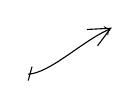
\begin{tikzpicture}[scale=.8]
\draw[->] (0,0) .. controls (.35,.02) and (.85,.52) .. (1.3,.72);
\draw (0,-.10)--(.06,.12);
\draw (.93,.71)--(1.31,.73)--(1.10,.45);
\end{tikzpicture}}

% E537-04
alors les hom induits par $\delta_G$
% E537-05
\[
(33)\qquad
\diagram{\begin{tikzcd}[ampersand replacement=\&,column sep=large]
Z_\rho\arrow[r,"{\delta_\rho}"]\&\gamma_{\rho,\sigma}
\end{tikzcd}},
\qquad
\diagram{\begin{tikzcd}[ampersand replacement=\&,column sep=large]
Z_\sigma\arrow[r,"{\delta_\sigma}"]\&\gamma_{\rho,\sigma}
\end{tikzcd}}
\]
% E537-06
ont
% E537-07
\deleted{comme}
% E537-08
\inserted{des}
images qui contiennent $\gamma'_{\rho,\sigma}$ et
$\gamma''_{\rho,\sigma}$ respectivement,
% E537-09
\deleted{et \unsure{sss|ssi} \unsure{à}}

% E537-10
\deleted{D'ailleurs l'image de $Z_\rho$ est contenue dans
$\gamma'_{\rho,\sigma}$
% E537-11
\deleted{si on suppose}
% E537-12
\inserted{(\unsure{ou égale}) \unsure{sss|ssi}}
$\rho$ et $\rho^{-1}$ non conjugués dans $\mathcal{G}$,
% E537-13
\deleted{il suffit}
% E537-14
\inserted{et de}
% E537-15
\deleted{\unsure{pour ceci}}
$\overline{\mathrm m}$ l'image de $Z_\sigma$ est
\unsure{réduite|réduit} à $\gamma''_{\rho,\sigma}$
\unsure{sss|ssi} $\sigma$ et $\sigma^{-1}=-\sigma$
non conjugués dans $\mathcal{G}$. Notons p.ex.
% E537-16
\deleted{que}
% E537-17
\inserted{si}
% E537-18
\deleted{$\mathcal{G}=\mathrm{SL}(2,\widehat{\mathbb{Z}})'$,}
$\sigma^2=1$,
\unsure{la} dernière condition n'est pas \unsure{satisfaite},
donc
% E537-19
$\diagram{\begin{tikzcd}[ampersand replacement=\&]
Z_\sigma\arrow[r]\&\gamma_{\rho,\sigma}
\end{tikzcd}}$
est surjective,
% E537-20
\deleted{elle ne}
% E537-21
\inserted{\deleted{\unsure{mais}} elle}
l'est
% E537-22
\deleted{pas non plus}
% E537-23
\deleted{\unsure{qu'elle est satisfaite si}}
$\mathcal{G}=\unsure{\mathrm{SL}}(2,\widehat{\mathbb{Z}})$
% E537-24
\inserted{dans $\mathrm{SL}(2,\widehat{\mathbb{Z}})$}
$\sigma$ y est conjugué à $-\sigma$, par le
% E537-25
\deleted{(car $\sigma$ et}
\unsure{th.} général de Steinberg p.ex.) ---
\unsure{se peut-il produire} dans le \unsure{cas}
universel $\mathrm{SL}(2,\mathbb{Z})^{\wedge}
=\mathcal{G}_{1,1}^{+\wedge}$?
}

% E537-26
\margin{\deleted{
La condition sur $\rho$ est non satisfaite
% E537-27
\deleted{\unsure{pour}}
$\mathcal{G}=\mathrm{SL}(2,\widehat{\mathbb{Z}})/\pm1$,
Comme dans ce cas les \uline{deux} hom
% E537-28
$\diagram{\begin{tikzcd}[ampersand replacement=\&,column sep=small]
Z_\rho,\deleted{\unsure{Z_\sigma}}\arrow[r]\&
\unsure{\widehat{\gamma}_{\rho,\sigma}|\gamma_{\rho,\sigma}}
=\widehat{\mathbb{Z}}^{*}
\end{tikzcd}}$,
% E537-29
$\diagram{\begin{tikzcd}[ampersand replacement=\&,column sep=small]
Z_\sigma\arrow[r]\&\gamma_{\rho,\sigma}=\widehat{\mathbb{Z}}^{*}
\end{tikzcd}}$
sont \unsure{surjections|surjectives}),
mais elle l'est pour $\mathcal{G}=\mathrm{SL}(2,\widehat{\mathbb{Z}})$,
car on trouve que l'image de
% E537-30
$\diagram{\begin{tikzcd}[ampersand replacement=\&,column sep=small]
\unsure{Z_\rho}\arrow[r]\&\gamma_{\rho,\sigma}
\end{tikzcd}}$
est $\gamma'_{\rho,\sigma}$.
Mais dans $\unsure{\mathcal{G}_{0,3}^{+\wedge}}$,
$\rho$ et $\rho^{-1}$ sont aussi non conjugués,
i.e. l'image est \unsure{réduite} aussi à $\gamma'_{\rho,\sigma}$.
}}
% E537-31
\margin{536}

% E537-F01
\margin{\begin{center}
536\\
\texttt{https://grothendieck.umontpellier.fr}\\
Université de Montpellier, UMR CNRS 5149, Case courrier 051, Place Eugène Bataillon\\
34095 Montpellier cedex 5 - France
\end{center}}
\scanpage{538}
% E538-01
\mspage{572}

% E538-02
\uline{Proposition} \quad 1°) L'image $\delta_\rho(Z_\rho)$ contient
$\gamma'_{\rho,\sigma}$, et est
% E538-03
\deleted{\unsure{ég}}
% E538-04
réduite à $\gamma'_{\rho,\sigma}$ \unsure{sss|ssi}
$\rho$ et $\rho^{-1}$ non conjugués dans $\mathcal{G}$ ---
donc elle est égale à $\gamma_{\rho,\sigma}$
i.e.
% E538-05
$\delta_\rho:\diagram{\begin{tikzcd}[ampersand replacement=\&,column sep=large]
Z_\rho\arrow[r]\&\gamma_{\rho,\sigma}
\end{tikzcd}}$
% E538-06
épi \unsure{sss|ssi} $\rho$ et $\rho^{-1}$ sont conjugués dans $\mathcal{G}$.

% E538-07
2°) L'image $\delta_\sigma(Z_\sigma)$ contient
$\gamma''_{\rho,\sigma}$, et elle est réduite à
$\gamma''_{\rho,\sigma}$ \unsure{sss|ssi} $\sigma$ et
$\sigma^{-1}=-\sigma$ non conjugués dans $\mathcal{G}$ ---
\unsure{donc|sinon} elle est égale à $\gamma_{\rho,\sigma}$ i.e.
% E538-08
$\delta_\sigma:\diagram{\begin{tikzcd}[ampersand replacement=\&,column sep=large]
Z_\sigma\arrow[r]\&\gamma_{\rho,\sigma}
\end{tikzcd}}$
% E538-09
épi \unsure{sss|ssi} $\sigma$ et
$\unsure{-\sigma^{-1}|\sigma^{-1}}=-\sigma$ sont conjugués dans $\mathcal{G}$.

% E538-10
\uline{Corollaire 1}. Si $\mathcal{G}$ contient comme quotient
% E538-11
\[
SL(2,\mathbb{Z}/3\mathbb{Z})',\quad\text{avec}\quad
\rho=\begin{pmatrix}0&1\\-1&1\end{pmatrix},\qquad
\sigma=\begin{pmatrix}0&-1\\1&0\end{pmatrix}
\]
% E538-12
$(\bmod\ \pm1)$, alors l'image de $\delta_\rho$ est
$\gamma'_{\rho,\sigma}$.

% E538-13
En effet, on voit que $\rho$ et $\pm\rho^{-1}$ ne sont
conjugués dans $\mathcal{G}$, car ils ne le sont
pas dans $SL(2,\mathbb{Z}/3\mathbb{Z})'$ ---
% E538-14
\deleted{\unsure{par ex.}\ \unsure{pour}}
% E538-15
\inserted{Vérifions le:}
% E538-16
$\rho$ et $-\rho^{-1}$ ont déjà des traces distinctes
$1$ et $-1$, $\unsure{\in}(\mathbb{Z}/3\mathbb{Z})^{\unsure{*}}$,
ils ne sont pas conjugués.

% E538-17
On a
% E538-18
\[
(\underbrace{\tau\sigma}_{\tau'_\infty})(\rho)=\rho^{-1},
\]
% E538-19
donc
% E538-26
\deleted{tous} les éléments de
% E538-20
\deleted{$f\in$}
% E538-21
$GL(2,\mathbb{Z}/3\mathbb{Z})$
% E538-22
\deleted{tels que}
% E538-23
qui conjuguent $\rho$ en $\rho^{-1}$ sont de la forme
$f\tau'_\infty$, où
% E538-24
$f=\unsure{c|b}\rho+d$, on \unsure{veut}
$\det(f\tau'_\infty)=1$ i.e. $\det(f)=-1$
$(\text{car }\det(\tau'_\infty)=-1)$,
i.e. $c^2+\unsure{cd}+d^2=-1$, impossible.
% E538-25
\margin{537}

% E538-F01
\margin{\begin{center}
537\\
\texttt{https://grothendieck.umontpellier.fr}\\
Université de Montpellier, UMR CNRS 5149, Case courrier 051, Place Eugène Bataillon\\
34095 Montpellier cedex 5 - France
\end{center}}
\scanpage{539}

% E539-01
\uline{Corollaire 2}\quad Si $\sigma^2=1$, alors
% E539-02
$\diagram{\begin{tikzcd}[ampersand replacement=\&,column sep=large]
Z_\sigma\arrow[r]\&\gamma_{\rho,\sigma}
\end{tikzcd}}$
% E539-03
est surjectif. Si Par contre $\mathcal{G}$ contient comme quotient
% E539-04
\deleted{$\mathbb{Z}/4\mathbb{Z}$}
% E539-05
$SL(2,\mathbb{Z}/4\mathbb{Z})$
$(\uline{\text{sans}}\ \prime\ !)$, avec $\rho,\sigma$ comme
\unsure{d'habitude}, alors
% E539-06
\[
\operatorname{Im}(\delta_\sigma)=\gamma''_{\rho,\sigma}.
\]

% E539-07
Il faut voir que $\sigma$ et $\sigma^{-1}=-\sigma$ non conjugués
dans $SL(2,\mathbb{Z}/4\mathbb{Z})$, en utilisant que
$\tau_\infty(\sigma)=\sigma^{-1}$, donc
% E539-08
\deleted{il f}
% E539-09
les \unsure{élts|élms} de $GL(2,\mathbb{Z}/4\mathbb{Z})$ qui
conjuguent $\sigma$ en $\sigma^{-1}$ sont les
% E539-10
\inserted{$g=f\tau_\infty$ avec}
% E539-11
$f=t\sigma+\unsure{u|n}$,
% E539-12
\deleted{\unsure{avec}}
% E539-13
et donc que $\det(g)=1$ signifie $\det f=-1$
i.e. $t^2+\unsure{u|n}^2=-1$, impossible.

% E539-14
\deleted{
Posons
% E539-15
\[
(34)\qquad
\left\{
\begin{aligned}
SZ_\rho&=
% E539-16
\inserted{\operatorname{Ker}\delta_\rho=}
Z_\rho\cap\mathcal{G}=\operatorname{Centr}_{\mathcal{G}}(\rho).\\
SZ_\sigma&=
% E539-17
\inserted{\operatorname{Ker}\delta_\sigma=}
Z_\sigma\cap\mathcal{G}=\operatorname{Centr}_{\mathcal{G}}(\sigma)\\
SB_{\rho,\sigma}&=\operatorname{Ker}\delta_B
=B_{\rho,\sigma}\cap\mathcal{G}=L_0.
\end{aligned}
\right.
\]
}

% E539-18
\deleted{
% E539-19
\[
(35)\qquad
\begin{aligned}
&S_0\unsure{\mathcal{M}|M}_{\rho,\sigma}
\subset B_{\rho,\sigma}\times\unsure{Z_\rho|N_\rho}
\times Z_\sigma\times\unsure{G_{\rho,\sigma}|\gamma_{\rho,\sigma}}\\
&\text{''}\\
&\bigl\{(u,a,b,U\unsure{\}|)}\ \bigm|\,
\delta_B(u)=\delta_G(U)=\delta_\sigma(b)
=\varepsilon_3(\mu)\delta_\rho(a)\bigr\}
\end{aligned}
\]
}
% E539-20
\margin{538}

% E539-F01
\margin{\begin{center}
538\\
\texttt{https://grothendieck.umontpellier.fr}\\
Université de Montpellier, UMR CNRS 5149, Case courrier 051, Place Eugène Bataillon\\
34095 Montpellier cedex 5 - France
\end{center}}
\scanpage{540}
% E540-01
\mspage{573}

% E540-02
% E540-03
Notons que d'après (2), \inserted{(4)}, on a
% E540-04
\[
(35)\qquad \tau_B \overset{\mathrm{dfn}}{=}(\tau,-1)\in B_{\rho,\sigma}
\]
% E540-05
Et évidemment $\tau_B\notin L_0=B_{\rho,\sigma}\cap\mathcal{G}$.
Donc on a un plongement
% E540-06
\[
(36)\qquad
\left\{
\begin{array}{l}
\diagram{\begin{tikzcd}[ampersand replacement=\&,column sep=large,row sep=small]
\mathcal{G}'=\{1,\tau\}.\mathcal{G} \arrow[r,hook] \& G_{\rho,\sigma}\\
\tau \arrow[r,mapsto] \& \tau_B\\
g \arrow[r,mapsto] \& g\quad\text{si }g\in\mathcal{G}
\end{tikzcd}}
\end{array}
\right.,
\]
% E540-07
\margin{\uline{NB} $\mathcal{G}'$ est un quotient de
$\mathrm{GL}(2,\mathbf{Z})^\wedge$, et $\tau$ y correspond à
l'image de l'élément
$\tau_\infty=\begin{pmatrix}-1&0\\0&1\end{pmatrix}$
de $\unsure{\mathrm{GL}(2,\mathbf{Z})}$.}

% E540-08
% E540-09
donc l'\unsure{autom} $\tau$ de $\mathcal{G}$ sera considéré comme
induit par \deleted{\unsure{l'élé}} $\operatorname{int}(\tau_B)$,
où $\tau_B$ est considéré lui-$\overline{\mathrm m}$ comme un
élément de $G_{\rho,\sigma}$.

% E540-10
% E540-11
\deleted{\illegible{2}} En relation avec l'égalité
% E540-12
\[
\tau_B(\sigma)=\sigma^{-1}\quad(=-\sigma)
\]
% E540-13
% E540-14
% E540-15
% E540-16
% E540-18
% E540-17
qui montre que $\tau_B$ normalise le sous-groupe
\inserted{$L_\sigma$} \inserted{engendré par $\sigma$}
(isomorphe à un quotient de $\mathbf{Z}/4\mathbf{Z}$),
\deleted{\unsure{groupe}} \inserted{donc}
\inserted{normalise $Z_\sigma=\operatorname{Centr}_{G_{\rho,\sigma}}(L_\sigma)$},
\deleted{\unsure{puis introduisons}} introduisons
% E540-19
\[
(37)\qquad
N_\sigma=\underset{(\text{$1/2$ direct})}{\{1,\tau_B\}.Z_\sigma},
\]
% E540-20
et l'hom. canonique
% E540-21
\[
(38)\qquad
\left\{
\begin{array}{l}
\diagram{\begin{tikzcd}[ampersand replacement=\&,column sep=large,row sep=small]
N_\sigma \arrow[r,"i_\sigma"] \& G_{\rho,\sigma} \& \&\\
\tau_B \arrow[r,mapsto] \& \tau_B, \& x \arrow[r,mapsto] \& x\quad\text{si }x\in Z_\sigma
\end{tikzcd}}
\end{array}
\right..
\]

% E540-22
\deleted{Cet hom. est injectif sss}
% E540-23
% E540-24
L'image de cet hom. n'est autre que le normalisateur de $\sigma$
dans $G_{\rho,\sigma}$, car un \deleted{\unsure{autom}}
$g\in G_{\rho,\sigma}$ qui normalise $L_\sigma$ doit transformer
$\sigma$ en un générateur de $L_\sigma$, i.e. en $\sigma$ ou
$\sigma^{-1}$, dans le premier cas on aura $g\in Z_\sigma$, dans
le deuxième $g(\sigma)=\tau_B(\sigma)$ i.e. $\tau_B^{-1}g\in Z_\sigma$
i.e. $g\in\tau_B Z_\sigma$. L'hom (38) est injectif

% E540-25
\margin{539}

% E540-F01
\margin{\begin{center}
539\\
\texttt{https://grothendieck.umontpellier.fr}\\
Université de Montpellier, UMR CNRS 5149, Case courrier 051, Place Eugène Bataillon\\
34095 Montpellier cedex 5 - France
\end{center}}
\scanpage{541}
% E541-01
\deleted{sss $\tau_B\in Z$}
% E541-02
sss $\tau_B\notin Z_\sigma$ i.e. $\sigma\ne\sigma^{-1}$ i.e.
$\sigma^2\ne1$ i.e. "$-1$" $\ne1$.

% E541-03
Puisqu'on y est, profitons de la formule
% E541-04
\[
\tau_B(\rho)=\sigma(\rho^{-1})
\]
% E541-05
pour introduire
% E541-06
\[
(39)\qquad
\tau'\uuline{=}\sigma^{-1}\tau\in\mathcal{G}'\subset G_{\rho,\sigma}
\]
% E541-07
(qui correspond à l'élément
% E541-08
% E541-09
\[
(40)\qquad
\tau'_\infty=\sigma_\infty^{-1}\tau_\infty
=-\sigma_\infty\tau_\infty
=\begin{pmatrix}0&1\\1&0\end{pmatrix}
\in\underbrace{\mathrm{GL}(2,\mathbf{Z})}_{
\inserted{\substack{\Vert\\\mathcal{T}_{1,1}}}}
\biggr),
\]

% E541-10
% E541-11
\deleted{\unsure{qui est}} on aura donc
% E541-12
\[
(40)\qquad \tau'^2=1,\qquad \tau'(\rho)=\rho^{-1}.
\]

% E541-13 deletion
\deleted{Introduisons donc}
% E541-14 deletion
\deleted{$(41)\qquad N_\rho=\{1,\tau'\}.$}
% E541-15
% E541-16
\inserted{Ainsi $\tau'$ normalise le sous-groupe $L_\rho$
(isomorphe à un quotient de $\mathbf{Z}/6\mathbf{Z}$) engendré
par $\rho$, donc il normalise le centralisateur
\inserted{$Z_\rho$} de $L_\rho$, et on peut construire}
% E541-17
% E541-18
\margin{\uline{NB} On a en $\overline{\mathrm m}$ temps
$\tau'(\sigma)=\sigma^{-1}$, donc on peut considérer $\tau'$
comme élément de $N_\sigma$, et \deleted{\illegible{1}} on a
$N_\sigma=\{1,\tau'\}.Z_\sigma$ (qui est $1/2$ direct)}
% E541-19
\[
(41)\qquad
N_\rho\overset{\mathrm{dfn}}{=}
\underset{(\text{semi-direct})}{\{1,\tau'\}.Z_\rho}
\]
% E541-20
% E541-21
% E541-22
et \deleted{\unsure{un}} \deleted{\unsure{du}} hom. canonique
% E541-23
\[
(42)\qquad
\left\{
\begin{array}{l}
\diagram{\begin{tikzcd}[ampersand replacement=\&,column sep=large,row sep=small]
N_\rho \arrow[r,"i_\rho"] \& G_{\rho,\sigma} \& \&\\
\tau' \arrow[r,mapsto] \& \tau', \& x \arrow[r,mapsto] \& x\quad\text{pour }x\in Z_\rho
\end{tikzcd}}
\end{array}
\right..
\]

% E541-24
% E541-25
% E541-26
% E541-27
L'image de cet hom. est le normalisateur de $L_\rho$ dans
$G_{\rho,\sigma}$ --- on le voit comme \unsure{t-à-l} pour $i_\sigma$,
en notant que \deleted{les}
\inserted{$\rho,\rho^{-1}$ sont les \uline{seuls}} générateurs de
$L_\rho$. L'hom $i_\rho$ est injectif sss $\tau'\notin Z_\rho$
i.e. \deleted{\unsure{sss}} $\rho\ne\rho^{-1}$ i.e. $\rho^2\ne1$
i.e. $\rho\ne-1$
% E541-28
% E541-29
% E541-30
% E541-31
% E541-32
(\deleted{\unsure{en ce cas}}
\inserted{NB \uline{$\rho=-1$}}
\deleted{\unsure{implique}} \deleted{\unsure{équivalent}}
\deleted{\unsure{en fait}} que $\rho$ commute à $\sigma$, et que
$\mathcal{G}$ est un quotient de $\mathbf{Z}/12\mathbf{Z}$, avec
$\rho$ correspondant à $2$
% E541-33 insertion
\inserted{et $\sigma$ à $3$, mais ici $2\rho=0$ donc
$\mathcal{G}$ est un quotient de $\mathbf{Z}/4\mathbf{Z}$ avec
$\rho$ correspondant à $2$, $\sigma$ à $3=-1\ldots$}).

% E541-34
% E541-35
\margin{
\[
(43)\qquad\left\{
\begin{array}{l}
\diagram{\begin{tikzcd}[ampersand replacement=\&,column sep=huge,row sep=large]
N_\rho \arrow[r,"\delta_\rho=\delta_G\circ i_\rho"] \& \gamma_{\rho,\sigma}\\
N_\sigma \arrow[r,"\delta_\sigma=\delta_G\circ i_\sigma"] \& \gamma_{\rho,\sigma}
\end{tikzcd}}\\
\hfill\text{épimorphismes}
\end{array}
\right.
\]}
% E541-36
\margin{"On a fait ce qu'il fallait" pour avoir des
\uline{épimorph.} $\unsure{\varphi}$.}
% E541-37
\margin{540}

% E541-F01
\margin{\begin{center}
540\\
\texttt{https://grothendieck.umontpellier.fr}\\
Université de Montpellier, UMR CNRS 5149, Case courrier 051, Place Eugène Bataillon\\
34095 Montpellier cedex 5 - France
\end{center}}
\scanpage{542}
\mspage{574}
% E542-01
\deleted{\(\unsure{(43)}\)}
% E542-02
\unsure{Situons|Soit}
% E542-03
\deleted{\(\unsure{\mathfrak{g}|g}\)}

% E542-04
\[
(44)\qquad
\begin{gathered}
S\unsure{\mathfrak{g}|g}_{\rho,\sigma}^{\unsure{*}}
\subset \mathcal{G}'\times\mathcal{G}\times\widehat{\mathbb Z}^{*}
\\[-2pt]
\Vert\\[-2pt]
\left\{(\alpha,\beta,\mu)\ \left|
\begin{array}{l}
\alpha\equiv\tau^{\nu_3(\mu)}\bmod\mathcal{G}
\quad\text{i.e. }\chi(\alpha)=\varepsilon_3(\mu)\\
\underbrace{\alpha\rho(\alpha)^{-1}}_{\zeta}
=\underbrace{\varepsilon_2(\mu)\beta\sigma(\beta)^{-1}}_{\eta}
\ell_1^\nu,\quad\text{où}
\end{array}\right.\right\}
\end{gathered}
\]
% E542-05
\inserted{\[
\nu=(\mu-1)/2,\qquad\uline{(\ell_1=\varepsilon_1^2)}
\]}

% E542-06
\deleted{\[
(\unsure{36})\qquad
\unsure{\mathfrak{g}|g}_{\rho,\sigma}^{\unsure{*}\,\mathrm{eff}}
=\left\{(\alpha,\beta,\mu)\in
\unsure{\mathfrak{g}|g}_{\rho,\sigma}^{*}\ \middle|\ \unsure{\exists}\right.
\]}

% E542-07
d'où

% E542-08
% E542-09
\[
(45)
\]
\diagram{\(
\left\{
\begin{gathered}
\begin{tikzcd}[ampersand replacement=\&,column sep=large]
S\unsure{\mathfrak{g}|g}_{\rho,\sigma}^{\unsure{*}}
\arrow[r] \&
\begin{gathered}
\Sigma_{\rho,\sigma}\subset\mathcal{G}\times\mathcal{G}\times\widehat{\mathbb Z}^{*}\\[-2pt]
\Vert\quad\mathrm{dfn}\\[-2pt]
\left\{(\zeta,\eta,\mu)\ \left|
\begin{array}{l}
\zeta\rho\ \text{conj. ds }\mathcal{G}:\rho^\mu\\
\unsure{\eta|\zeta}\sigma\quad\underline{\hspace{7em}}\quad\sigma^\mu\\
\zeta=\deleted{\unsure{\beta\sigma(\beta)^{-1}}}\eta\ell_1^\nu
\end{array}\right.\right.
\end{gathered}\\
(\alpha,\beta,\mu)\arrow[r,mapsto]\&
\left(\overbrace{\alpha\rho(\alpha)^{-1}}^{[\alpha,\rho]},
\varepsilon_2(\mu)\overbrace{\beta\sigma(\beta)^{-1}}^{[\beta,\sigma]},\mu\right).
\end{tikzcd}
\end{gathered}
\right.
\)}
% E542-10
\inserted{\((\text{où }\nu=(\mu-1)/2\)}
% E542-11
On désigne par
\(\unsure{\mathfrak{g}|g}_{\rho,\sigma}^{\unsure{*}\,\mathrm{eff}}\)
l'image inverse de
\(\Sigma_{\rho,\sigma}^{\mathrm{eff}}\)
(cf cor. p. 570). \(\simeq B_{\rho,\sigma}\).
Par \unsure{construction}
% E542-12
\inserted{on trouve donc une application \uline{surjective}}
% E542-13
\margin{
\((\unsure{46\mathrm{bis}})\)
\diagram{\begin{tikzcd}[ampersand replacement=\&]
S\unsure{\mathfrak{g}|g}_{\rho,\sigma}^{\mathrm{eff}}
\arrow[r,"\text{épi.}"]\&
\Sigma_{\rho,\sigma}^{\mathrm{eff}}
\end{tikzcd}}
}

% E542-14
On considère
\(S\unsure{\mathfrak{g}|g}_{\rho,\sigma}^{*}\)
comme contenu dans un
% E542-15
\deleted{groupe}
% E542-16
\inserted{ens.}
% E542-17
plus gros

% E542-18
% E542-19
\[
(47)\qquad
\begin{gathered}
\unsure{\mathfrak{g}|g}_{\rho,\sigma}^{\unsure{*}}
\subset G_{\rho,\sigma}\times G_{\rho,\sigma}
\times\widehat{\mathbb Z}^{*}
\\[-2pt]
\Vert\\[-2pt]
\left\{(\alpha,\beta,\mu)\ \left|
\begin{array}{l}
\chi(\alpha)\equiv\varepsilon_3
\bigl(\deleted{\unsure{\chi(\mu)|\chi(\beta)}}\mu\bigr)
\chi(\beta);\\
\underbrace{\alpha\rho(\alpha)^{-1}}_{=\alpha(\rho)\rho^{-1}=\zeta}
=
\underbrace{\varepsilon_2(\mu)\beta\sigma(\beta)^{-1}}_
{=\varepsilon_2(\mu)\beta(\sigma)\sigma^{-1}=\eta}
\ell_1^\nu
\end{array}\right.\right\}
\end{gathered}
\]
% E542-20
de sorte que l'on aura
% E542-21
% E542-22
\[
(48)\qquad
\begin{aligned}
S\unsure{\mathfrak{g}|g}_{\rho,\sigma}^{\unsure{*}}
&=\unsure{\mathfrak{g}|g}_{\rho,\sigma}^{\unsure{*}}
\cap\bigl(\mathcal{G}'\times\mathcal{G}\times\widehat{\mathbb Z}^{*}\bigr),
\\
&=\left\{(\alpha,\beta,\mu)\in
\unsure{S\mathfrak{g}|Sg}_{\rho,\sigma}^{*}
\ \left|
\begin{array}{l}
\delta_\sigma(\beta)=1\deleted{\unsure{\}}}\\
\delta_\rho\bigl(\alpha\tau^{\nu_3(\mu)}\bigr)=1
\end{array}\right.\right\}
\end{aligned}
\]
% E542-23
\margin{541}

% E542-F01
\margin{\begin{center}
541\\
\texttt{https://grothendieck.umontpellier.fr}\\
Université de Montpellier, UMR CNRS 5149, Case courrier 051, Place Eugène Bataillon\\
34095 Montpellier cedex 5 - France
\end{center}}
\scanpage{543}
% E543-01
et on a encore une application canonique
% E543-02
\[
(49)
\]
\diagram{\(
\left\{
\begin{gathered}
\begin{tikzcd}[ampersand replacement=\&,column sep=large]
\unsure{\mathfrak{g}|g}_{\rho,\sigma}^{*}\arrow[r]\&
\Sigma_{\rho,\sigma}^{\unsure{*}}\\
(\alpha,\beta,\mu)\arrow[r,mapsto]\&
\bigl([\alpha,\rho],\varepsilon_2(\mu)[\beta,\sigma],\mu\bigr).
\end{tikzcd}
\end{gathered}
\right.
\)}

% E543-03
\deleted{\unsure{dont l'i}}
% E543-04
On note
\(\unsure{\mathfrak{g}|g}_{\rho,\sigma}^{\mathrm{eff}}\)
l'image inverse de
\(\Sigma_{\rho,\sigma}^{\mathrm{eff}}\),
et on trouve
% E543-05
\[
(50)\qquad
\begin{aligned}
S\unsure{\mathfrak{g}|g}_{\rho,\sigma}^{\mathrm{eff}}
&=\unsure{\mathfrak{g}|g}_{\rho,\sigma}^{\mathrm{eff}}
\cap\bigl(\mathcal{G}'\times\mathcal{G}\times\widehat{\mathbb Z}^{*}\bigr)
\\
&=\left\{(\alpha,\beta,\mu)\in
\unsure{\mathfrak{g}|g}_{\rho,\sigma}^{\mathrm{eff}}
\ \left|
\begin{array}{l}
\delta_\sigma(\beta)=1\\
\unsure{\delta_\rho|\delta_B}\bigl(\alpha{\tau'}^{\nu_3(\mu)}\bigr)=1
\end{array}\right.\right\}
\end{aligned}
\]

% E543-06
On a une section de
% E543-07
% E543-08
% E543-09
% E543-10
\[
(51)
\]
\diagram{
\begin{tikzcd}[ampersand replacement=\&,column sep=large,row sep=large]
\unsure{\mathfrak{g}|g}_{\rho,\sigma}^{\mathrm{eff}}\arrow[r]\&
\Sigma_{\rho,\sigma}^{\mathrm{eff}}\&
\zeta=[u,\rho],\overset{\inserted{\eta=}}{[u,\sigma]},
\overset{\inserted{\mu=}}{\chi_B(u)}
\\
\& B_{\rho,\sigma}
\arrow[u,"\sim"']
\arrow[ul,"\text{\uline{section}}"]\&
u\deleted{\unsure{\varphi|*}}\arrow[u,mapsto]
\end{tikzcd}
}

% E543-11
donnée par
% E543-12
% E543-13
% E543-14
\[
(52)
\]
\diagram{\begin{tikzcd}[ampersand replacement=\&,column sep=large]
u\deleted{\unsure{\varphi|*}}\arrow[r,mapsto]\&
\bigl(\deleted{\unsure{\alpha=}}u,\,
u{\tau'}^{\nu_2(\mu)},\,\mu=\chi_B(u)\bigr)
\end{tikzcd}}

% E543-15
puisqu'on aura
(posant \(\varepsilon=\varepsilon_2(\mu)
\unsure{\overset{\mathrm{dfn}}{=}|=}
(-1)^{\nu_2}\).)
% E543-16
\[
[u,\rho]=u\rho(u)^{-1}=\zeta
\]
% E543-17
\[
\begin{aligned}
\varepsilon
\left[u{\tau'}^{\nu_2(\mu)=\nu_2},\sigma\right]
&=\varepsilon u{\tau'}^{\nu_2}
\sigma\bigl(u\unsure{\tau|\tau'}^{\nu_2}\bigr)^{-1}\\
&=\varepsilon u
\left(\underbrace{
\unsure{\tau|\tau'}^{\nu_2}
\sigma\bigl(\unsure{\tau|\tau'}^{\nu_2}\bigr)^{-1}
}_{=\varepsilon}\right)\sigma(u)^{-1}
=\unsure{\varepsilon u|u}\sigma(u)^{-1}=\eta
\end{aligned}
\]
% E543-18
OK. Donc
% E543-19
\deleted{\unsure{l'ens|les}}
% E543-20
% E543-21
\inserted{l'ens \deleted{\unsure{des}}
\(\unsure{\mathfrak{g}_{\rho,\sigma}(u,\mu)|g_{\rho,\sigma}^{(u,\mu)}}\)}
% E543-27
des \((\alpha,\beta,\mu)\,\unsure{-}\)
donnant \unsure{l'image}
% E543-22
% E543-23
% E543-24
\[
(\zeta,\eta,\mu)\deleted{\unsure{\Longrightarrow|=}}
\unsure{[|(}\,[u,\rho],[u,\sigma],
\overset{\inserted{\mu=}}{\chi_B(u)}\bigr)
\]
% E543-25
\unsure{sera exactement}
% E543-26
\margin{542}

% E543-F01
\margin{\begin{center}
542\\
\texttt{https://grothendieck.umontpellier.fr}\\
Université de Montpellier, UMR CNRS 5149, Case courrier 051, Place Eugène Bataillon\\
34095 Montpellier cedex 5 - France
\end{center}}
\scanpage{544}
\mspage{575}
% E544-01
\deleted{\unsure{les}}
% E544-02
\inserted{\(
\unsure{\mathfrak{g}_{\rho,\sigma}(u,\mu)|g_{\rho,\sigma}^{(u,\mu)}}
=
\)}
% E544-03
\[
(53)\qquad
\left\{\left(
\overbrace{ua_0^{-1}}^{\alpha},
\overbrace{u{\tau'}^{\nu_2}b_0^{-1}}^{\unsure{\beta|b}},
\mu\right)
\ \middle|\ a_0\in Z_\rho,\ b_0\in Z_\sigma,\
\nu_2=\nu_2(\mu)\right\}
\]
% E544-04
\inserted{\[
\bigl(=(ua_0^{-1},ub^{-1},\mu)\unsure{\}}
\quad\text{où}\quad b=b_0{\tau'}^{\unsure{\nu_2}}
\]}
% E544-05
qu'on écrit aussi
% E544-06
% E544-29
\[
(54)\qquad
\unsure{\mathfrak{g}_{\rho,\sigma}(u,\mu)|g_{\rho,\sigma}^{(u,\mu)}}
=
\left\{\left(
\underbrace{ua_0^{-1}}_{\alpha},
\underbrace{u\,i_\sigma(b)}_{\beta},
\mu\right)
\ \middle|\ 
a_0\in Z_\rho,\ 
\underset{\inserted{\text{(cf (37)(38))}}}{b\in N_\sigma},\
\boxed{\varepsilon_\sigma(b)=\varepsilon_2(\mu)}
\right\}
\]
% E544-07
où \(\varepsilon_\sigma:N_\sigma\longrightarrow\{\pm1\}\)
est défini sur (37) comme l'hom. can.
s'insérant dans la suite exacte
% E544-08
\[
(55)
\]
\diagram{\begin{tikzcd}[ampersand replacement=\&]
1\arrow[r]\&Z_\sigma\arrow[r]\&N_\sigma
\arrow[r,"\varepsilon_\sigma"]\&
\underbrace{\{\pm1\}}_{\simeq\{1,\tau'\}}\arrow[r]\&1.
\end{tikzcd}}

% E544-09
Si on cherche l'ens des éléments de
\(S\unsure{\mathfrak{g}|g}_{\rho,\sigma}^{\mathrm{eff}}\)
au dessus de \((\zeta,\eta,\mu)\), il faut de plus
imposer les conditions
% E544-10
\[
(56)\qquad
\deleted{\unsure{\alpha=}}ua_0^{-1}{\tau'}^{\nu_3(\mu)}\in\mathcal{G},
\quad u\,i_\sigma(b)\in\mathcal{G}
\]
% E544-11
i.e.
\[
\delta_G(ua_0^{-1}{\tau'}^{\nu_3})=1,\quad
\delta_G(u\,i_\sigma(b))=1
\]
% E544-12
soit encore
% E544-13
\[
(57)\qquad
\delta_G(u)=
\underbrace{\delta_\sigma(b)}_{\text{cf (43)}}
=
\underbrace{\delta_\rho}_{\text{cf (43)}}
({\tau'}^{\nu_3}.a_0).
\]
% E544-14
Posons donc
\[
a={\tau'}^{\nu_3}.a_0\quad\text{\unsure{ds|dans}}\ N_\rho
\]
% E544-15
\inserted{\((\text{donc }a_0={\tau'}^{\nu_3}a)\)}
% E544-16
on voit que
% E544-17
\[
(54)\qquad
\unsure{\mathfrak{g}_{\rho,\sigma}(u,\mu)|g_{\rho,\sigma}^{(u,\mu)}}
=
\left\{(ua^{-1}{\tau'}^{\nu_3},ub^{-1},\mu)\ \left|
\begin{array}{l}
a\in N_\rho,\ b\in N_\sigma\ \text{tels que}\\
\varepsilon_\rho(a)=\varepsilon_3(\mu),\
\varepsilon_\sigma(b)=\varepsilon_2(\mu)\\
\delta_\rho(a)=\delta_\sigma(b)=\delta_G(u)
\end{array}\right.\right\}
\]

% E544-18
Introduisons donc le groupe
% E544-19
% E544-20
\[
(55)\qquad
\deleted{\unsure{S_0}}
\unsure{\mathcal{M}|M}_{\rho,\sigma}[0]
=\unsure{B}_{\rho,\sigma}
\times_{\gamma_{\rho,\sigma}}N_\rho
\times_{\gamma_{\rho,\sigma}}N_\sigma.
\]
% E544-21
et les homomorphismes composés
% E544-22
% E544-23
% E544-24
\[
(56)
\]
\diagram{\(
\left\{
\begin{gathered}
\begin{tikzcd}[ampersand replacement=\&,column sep=large]
\deleted{\unsure{S_0}}\unsure{\mathcal{M}|M}_{\rho,\sigma}[0]
\arrow[r]\&N_\rho\&
\overset{\varepsilon_\rho}{\unsure{\longleftrightarrow|\longrightarrow}}\&
\{\pm1\}
\\
\deleted{\unsure{S_0}}\unsure{\mathcal{M}|M}_{\rho,\sigma}[0]
\arrow[r]\&N_\sigma\arrow[rr,"\varepsilon_\sigma"]\&\&
\{\pm1\}
\end{tikzcd}
\end{gathered}
\right.
\)}
% E544-25
% E544-28
\margin{\deleted{\unsure{notés}\ \(\varepsilon'_\rho\)}}
% E544-26
(encore notés \(\varepsilon_\rho,\varepsilon_\sigma\)
par abus de notation)
% E544-27
\margin{543}

% E544-F01
\margin{\begin{center}
543\\
\texttt{https://grothendieck.umontpellier.fr}\\
Université de Montpellier, UMR CNRS 5149, Case courrier 051, Place Eugène Bataillon\\
34095 Montpellier cedex 5 - France
\end{center}}
\scanpage{545}
% E545-01
et

% E545-02
% E545-03
\noindent(57)\quad
\diagram{\begin{tikzcd}[ampersand replacement=\&,column sep=large]
\deleted{\unsure{S_0}}M_{\rho,\sigma}[0]
  \arrow[r,"\delta_{SM}"]
\& \gamma_{\rho,\sigma} \arrow[r,"\chi_\gamma"]
\& \widehat{\mathbb Z}^{*}
\end{tikzcd}}
soit $\chi_{SM}$, (ou \unsure{simplem$^{t}$|simplement} $\chi$)

% E545-04
considérons

% E545-05
% E545-06
\noindent(58)\quad
\diagram{\begin{tikzcd}[ampersand replacement=\&,column sep=huge]
\deleted{\unsure{S_0}}M_{\rho,\sigma}[0]
 \arrow[r,"{\varepsilon_{\rho,\sigma}=(\unsure{\varepsilon_\sigma},\varepsilon_\rho)}"]
\& \{\pm1\}\times\{\pm1\}
\end{tikzcd}}

% E545-07
et

% E545-08
% E545-09
\noindent(59)\quad
\diagram{\begin{tikzcd}[ampersand replacement=\&,column sep=huge]
\deleted{\unsure{S_0}}M_{\rho,\sigma}[0]
 \arrow[r,"{\varepsilon_{2,3}:x\longmapsto(\unsure{\varepsilon_2}(\chi(x)),\varepsilon_3(\chi(x)))}"]
\& \{\pm1\}\times\{\pm1\}
\end{tikzcd}}

% E545-10
et considérons le sous-groupe des coïncidences des deux hom. précédents

% E545-11
% E545-12
% E545-13
% E545-14
\[
\begin{aligned}
(60)\quad
\deleted{\unsure{S_0}}M_{\rho,\sigma}^{\unsure{\mathrm{eff}}}[0]
 &\overset{\mathrm{dfn}}=
 \{x\in\unsure{S_0\{M_{\rho,\sigma}\}}\mid
 \varepsilon_{\rho,\sigma}(x)=\varepsilon_{2,3}(x)\}
\\
 &=\left\{\left(
 \underset{\substack{\rotatebox{90}{$\in$}\\ B_{\rho,\sigma}}}{u},
 \underset{\substack{\rotatebox{90}{$\in$}\\ N_\rho}}{a},
 \underset{\substack{\rotatebox{90}{$\in$}\\ Z_\sigma}}{b}
 \right)\ \middle|\
 \begin{gathered}
 \delta_B(u)=\delta_\rho(a)=\delta_\sigma(b)
 \quad\text{soit }\Delta\in\gamma_{\rho,\sigma}\\
 \varepsilon_\rho(a)=
 \deleted{\unsure{\varepsilon_3(\chi_B(u))}}
 \inserted{\varepsilon_3(\chi_\gamma(\Delta))},
 \quad\varepsilon_\sigma(b)=\varepsilon_2(\chi_\gamma(\Delta))
 \end{gathered}
 \right.
\end{aligned}
\]

% E545-15
On a une application naturelle

% E545-16
\noindent(61)\quad
\diagram{\begin{tikzcd}[ampersand replacement=\&,column sep=huge]
M_{\rho,\sigma}^{\mathrm{eff}}[0] \arrow[r]
 \& \mathcal G'\times\mathcal G\times\widehat{\mathbb Z}^{*}\\
(u,a,b)\arrow[r,mapsto] \& (\alpha,\beta,\mu)
\end{tikzcd}}
, avec
$\begin{gathered}
\alpha=ua^{-1}\tau'^{\nu_\rho(a)}\\
\beta=ub^{-1}\\
\mu=\chi_B(u)=\chi_\rho(a)=\chi_\sigma(b)
\end{gathered}$

% E545-17
\margin{\uline{NB} on a identifié $a\in N_\rho$, $b\in N_\sigma$
\unsure{à leurs images} $i_\rho(a)$, $i_\sigma(b)$ dans $G_{\rho,\sigma}$.}

% E545-18
% E545-19
\margin{\uline{NB} On a posé \deleted{\unsure{(61)}}
$\nu_\rho(a)\in\mathbb Z/2$ tel que
$(-1)^{\nu_\rho(a)}=\varepsilon_\rho(a)$}

% E545-20
et on a fait ce qu'il fallait pour que celle-ci soit \unsure{injective}
et ait comme image $S\unsure{\mathfrak{g}|g}_{\rho,\sigma}^{\mathrm{eff}}$, donc induise une bijection

% E545-21
\noindent(62)\quad
\diagram{\begin{tikzcd}[ampersand replacement=\&,column sep=large]
M_{\rho,\sigma}^{\mathrm{eff}}[0] \arrow[r,"\sim"]
 \& S\unsure{\mathfrak{g}|g}_{\rho,\sigma}^{\mathrm{eff}}.
\end{tikzcd}}

% E545-22
% E545-23
\uline{Remarque}. En fait \inserted{les formules pour} (61)
\unsure{définissent} même une application

% E545-24
\noindent(62)\quad
\diagram{\begin{tikzcd}[ampersand replacement=\&,column sep=large]
M_{\rho,\sigma}[0]\arrow[r]
\&\mathcal G'\times\mathcal G\times\widehat{\mathbb Z}^{*}
\end{tikzcd}}

% E545-25
et pour un $(u,a,b)\in M_{\rho,\sigma}[0]$, son image $(\alpha,\beta,\mu)$
est liée à $u\in B_{\rho,\sigma}$ par les formules

% E545-26
\margin{544}

% E545-F01
\margin{\begin{center}
544\\
\texttt{https://grothendieck.umontpellier.fr}\\
Université de Montpellier, UMR CNRS 5149, Case courrier 051, Place Eugène Bataillon\\
34095 Montpellier cedex 5 - France
\end{center}}
\scanpage{546}
\mspage{576}

% E546-01
% E546-02
% E546-03
\[
(63)\quad
\left\{\begin{aligned}
u(\rho)&=\operatorname{int}(\alpha)(\rho)
&&\bigl(\inserted{\mathcal G-}\text{conjugué à }\rho^{\unsure{\varepsilon'}},
\text{ où }\varepsilon'=\varepsilon_\rho(a)\bigr)\\
u(\sigma)&=\varepsilon\operatorname{int}(\beta)(\sigma)
&&\bigl(\mathcal G\text{-conjugué à }\sigma^\varepsilon,
\text{ où }\varepsilon=\varepsilon_\sigma(b)\bigr)\\
&\deleted{\unsure{\alpha}}
\end{aligned}\right.
\]

% E546-04
(mais sans qu'on ait nécessairement
$\varepsilon'=\varepsilon_3(\mu)$, $\varepsilon=\varepsilon_2(\mu)$).

% E546-05
% E546-06
Ceci suggère une définition d'un groupe un peu plus gros que $B_{\rho,\sigma}$,
dans lequel $B_{\rho,\sigma}$ \unsure{sera} \inserted{inclus}
comme sous-gr. \unsure{inv.|$\triangleleft$} \unsure{d'index|d'indice}
$1,2$ ou $4$ --- et qui aura l'avantage, dans les ``bons cas'', d'être le groupe
des pts adéliques d'un schéma en groupes \unsure{convenable} sur $\mathbb Z$.

% E546-07
% E546-08
D'autre part, pour \deleted{\unsure{tuer}} éliminer le signe
$\varepsilon$ dans (63), (qui est présent $\unsure{\overline{\mathrm m}}$ si
$(u,a,b)\in M_{\rho,\sigma}[0]^{\mathrm{eff}}$), j'ai envie de remplacer $\beta$ par

% E546-09
\deleted{$\unsure{\beta'}=\tau'^{\nu}\beta'$, où
$\nu\in\mathbb Z/2$ \unsure{est lié}}

% E546-10
\[
(64)\quad \beta'=\tau'^{\nu}\beta
\qquad\left(\text{où }\nu\in\mathbb Z/2\mathbb Z\text{ lié par }
(-1)^\nu=\varepsilon\right)
\]

% E546-11
De sorte qu'on aura

% E546-12
\[
(65)\quad \deleted{\unsure{\varepsilon|\chi}}u(\sigma)=\operatorname{int}(\beta')(\sigma)
\quad\text{i.e.}\quad [u,\sigma]=\beta'\sigma(\beta')^{-1}.
\]

% E546-13
Ceci est lié à la convention \unsure{qu'un|qui un}
$u\in\Gamma_{\mathbb Q}^{\sim}$, que nous repérions par le couple
$(\alpha,\beta)\in\widehat{\Pi}_{0,3}'\times\widehat{\Pi}_{0,3}$,
sera désormais repéré par le couple
$(\alpha,\beta')\in\widehat{\Pi}_{0,3}\times\widehat{\Pi}_{0,3}'$, avec

% E546-14
\[
(66)\quad\unsure{\chi}(\alpha)=\varepsilon_3(\mu),
\quad\chi(\beta')=\varepsilon_2(\mu)
\qquad\bigl(\text{où }\mu=\chi(u)\text{ est le multiplicateur}\bigr)
\]

% E546-15
% E546-16
% E546-17
ce qui \deleted{donne} pour l'opération de $u$ sur
\deleted{$\unsure{\mathcal G_{0,3}^{+\wedge}}$}

% E546-18
\[
\mathcal G_{0,3}^{+\wedge}
=\mathrm{SL}(2,\mathbb Z)^{\wedge\unsure{\textcircled{1}}}
=\mathrm{SL}(2,\mathbb Z)^{\wedge}/\pm1
\]

% E546-19
ne change pas en réalité les formules particulières :

% E546-20
% E546-21
\[
(67)\quad\left\{\begin{aligned}
u(\rho)&=\operatorname{int}(\alpha).\rho,\quad
u(\sigma)=\operatorname{int}(\beta)\sigma
\quad(=\operatorname{int}(\beta').\sigma)\\
\alpha\rho(\alpha)^{-1}
&=\beta\underset{\deleted{\unsure{\varepsilon}}}{\unsure{\sigma}}(\beta)^{-1}\ell_1^\nu
\quad(=\beta'\sigma(\beta')^{-1}\ell_1^\nu)
\end{aligned}\right.
\qquad\nu=\frac{\mu-1}{2}
\]

% E546-22
\margin{545}

% E546-F01
\margin{\begin{center}
545\\
\texttt{https://grothendieck.umontpellier.fr}\\
Université de Montpellier, UMR CNRS 5149, Case courrier 051, Place Eugène Bataillon\\
34095 Montpellier cedex 5 - France
\end{center}}
\scanpage{547}

% E547-01
% E547-02
mais pour l'opération dans
\deleted{$\unsure{\mathcal G=\mathcal T_{1,1}}$}

% E547-03
$\mathcal T_{1,1}^{+\wedge}\simeq\mathrm{SL}(2,\mathbb Z)^{\wedge}$
lui-même donne des formules plus simples, savoir, au lieu de

% E547-04
\[
(68)\quad\left\{\begin{aligned}
u(\rho)&=\operatorname{int}(\alpha)\rho\qquad
u(\sigma)=\varepsilon.\operatorname{int}(\beta)\sigma\\
\alpha\rho(\alpha)^{-1}&=\varepsilon\beta\sigma(\beta)^{-1}\ell_1^\nu
\end{aligned}\right.,
\]

% E547-05
les formules plus sympathiques

% E547-06
\[
(69)\quad\left\{\begin{aligned}
u(\rho)&=\operatorname{int}(\alpha)\rho,\qquad
u(\sigma)=\operatorname{int}(\beta')(\sigma)\\
\alpha\rho(\alpha)^{-1}&=\beta'\sigma(\beta')^{-1}\ell_1^\nu
\end{aligned}\right.,
\]

% E547-07
où le signe $\varepsilon=\varepsilon_2(\mu)$ a disparu. Il apparaît dans les formules

% E547-08
\[
(70)\quad\chi(\alpha)=\varepsilon_3(\mu),\quad
\chi(\beta')=\varepsilon_2(\mu).
\]

% E547-09
Il me semble en avoir assez pour pouvoir reprendre ``à main levée'' les
constructions précédentes et les \unsure{achever} avec des notations plus adéquates.

% E547-10
% E547-11
% E547-12
Le groupe $\mathcal G'$
\inserted{quotient de $\mathcal T_{1,1}^{\wedge}\simeq\mathrm{GL}(2,\mathbb Z)^{\wedge}$}
prend d'ailleurs une importance croissante dans nos calculs, c'est lui qui mérite
\deleted{\unsure{aussi}} la notation simple $\mathcal G$, le sous-groupe fermé
engendré par $\rho,\sigma$ devenant $\mathcal G^{+}$ --- il correspond à
$\mathcal T_{1,1}^{+\wedge}\simeq\mathrm{SL}(2,\unsure{\widehat{\mathbb Z}|\mathbb Z})^{\wedge}$.

% E547-13
On supposera simplement que $\tau\notin\mathcal G^{+}$
($\tau$ étant l'image de $\tau_\infty$), ou ce qui revient au
$\overline{\mathrm m}$, que

% E547-14
\[
(71)\quad\tau'\notin\mathcal G^{+}
\]

% E547-15
\margin{546}

% E547-F01
\margin{\begin{center}
546\\
\texttt{https://grothendieck.umontpellier.fr}\\
Université de Montpellier, UMR CNRS 5149, Case courrier 051, Place Eugène Bataillon\\
34095 Montpellier cedex 5 - France
\end{center}}
\scanpage{548}
\mspage{577}

% E548-01
% E548-02
C'est finalement cet élément, qui normalise à la fois $L_\rho$ et $L_\sigma$
\deleted{\unsure{par}} \unsure{via} les formules remarquables

% E548-03
\[
(*)\quad \tau'(\rho)=\rho^{-1},\qquad \tau'(\sigma)=\sigma^{-1}
\]

% E548-04
qui prend le pas sur $\tau$, qui satisfait à

% E548-05
\[
(**)\quad \tau(\varepsilon_0)=\varepsilon_0^{-1},\qquad
\tau(\varepsilon_1)=\varepsilon_1^{-1}
\quad\text{et même }\tau(\sigma)=\sigma^{-1}
\]

% E548-06
(ce qui est évidemment très \unsure{vertueux} !), \unsure{mais} dont l'action sur $\rho$

% E548-07
\[
\tau(\rho)=\sigma(\rho^{-1})
\]

% E548-08
\unsure{est} moins commode.

% E548-09
\margin{Néanmoins $\tau'$ a sur $\tau$ le désavantage sérieux de ne pas être
\unsure{élément} du groupe
$\widehat{\Pi}'_{0,3}=\{1,\tau\}.\widehat{\Pi}_{0,3}$, où on a la relation de rigidité
$\widehat{\Pi}_{0,3}^{\prime\sigma}=\widehat{\Pi}_{0,3}^{\unsure{\prime}\rho}=\{1\}$
--- alors que dans $\{\unsure{1},\tau'\}.\widehat{\Pi}_{0,3}$, le centralisateur de
$\sigma$ n'est pas réduit à $1$, mais est égal à $\{1,\tau'\}$
De plus, $\tau'$ a le désavantage de ne pas être dans
$\unsure{\mathcal M}_{0,3}^{\unsure{!|\prime}}$ \dots}

% E548-10
\[\overline{\underline{\mathrm V}}\]

% E548-11
\margin{\uline{Données}\par\uline{préliminaires}}

% E548-12
$1^\circ)$ Soit donc $\mathcal G$ un groupe profini, muni d'un hom surjectif

% E548-13
\[\unsure{=|\to}\]

% E548-14
\noindent(1)\quad
\diagram{\begin{tikzcd}[ampersand replacement=\&,column sep=large]
\mathcal T_{1,1}^{\unsure{*|+}\wedge}\simeq\mathrm{GL}(2,\mathbb Z)^{\wedge}
\arrow[r,"\text{épi}"] \& \mathcal G
\end{tikzcd}},

% E548-15
ce que nous exprimerons par la donnée des trois générateurs topologiques
$\rho,\sigma,\tau'\in\mathcal G$, satisfaisant

% E548-16
\[
(2)\quad \rho^6=\sigma^4=\tau'^2=1,\quad
\begin{gathered}\rho^3=\sigma^2\\\text{(noté }-1\text{)}\end{gathered},\quad
\tau'\rho\tau'^{-1}=\rho^{-1},\quad
\tau'\sigma\tau'^{-1}=\sigma^{-1}.
\]

% E548-17
On désigne par $\mathcal G^+$ le sous-groupe fermé engendré par $\rho,\sigma$,
qui est donc l'image de

% E548-18
\[
\mathcal T_{1,1}^{+\wedge}\simeq\mathrm{SL}(2,\mathbb Z)^{\wedge},
\]

% E548-19
\margin{547}

% E548-F01
\margin{\begin{center}
547\\
\texttt{https://grothendieck.umontpellier.fr}\\
Université de Montpellier, UMR CNRS 5149, Case courrier 051, Place Eugène Bataillon\\
34095 Montpellier cedex 5 - France
\end{center}}
% ===== LM_C3-549-567: second pass, checked against the scans =====
\scanpage{549}

et on suppose que $\mathcal{G}^+\ne\mathcal{G}$, donc
\[
\tag{3}
\begin{gathered}
\mathcal{G}\simeq\{1,\tau'\}\mathbin{.}\mathcal{G}^+\\[-2pt]
(\tfrac12\ \text{direct})
\end{gathered}
\]
et on a une suite exacte canonique
\[
\tag{4}
\diagram{\begin{tikzcd}[column sep=large]
1\arrow[r]&\mathcal{G}^+\arrow[r]&\mathcal{G}\arrow[r,"\varepsilon_{\mathcal{G}}"]&\{\pm1\}\arrow[r]&1
\end{tikzcd}}
\]
On désigne aussi par $\nu_{\mathcal{G}}$ le composé
\[
\tag{5}
\diagram{\begin{tikzcd}[column sep=large,row sep=small]
\mathcal{G}\arrow[r,"\varepsilon_{\mathcal{G}}"]\arrow[rr,bend left=25,"\nu_{\mathcal{G}}"]&\{\pm1\}&\mathbb{Z}/2\mathbb{Z}\arrow[l,"\sim"']\\
&(-1)^\nu&\nu\arrow[l,mapsto]
\end{tikzcd}}\ .
\]

De façon générale, on \unsure{désignera} (par abus de langage) par une $\overline{\mathrm m}$ lettre des éléments de $\mathrm{Gl}(2,\mathbb{Z})$ --- tels $\varepsilon_0,\varepsilon_1,\tau=\tau_\infty,\tau'=\tau'_\infty$, $\sigma=\sigma_\infty,\rho=\rho_\infty$ etc --- et leurs images dans $\mathcal{G}$.

\margin{Les groupes $Z_{\rho,\sigma}$, $\gamma_{\rho,\sigma}$}

$2^\circ)$ Soit
\[
\tag{6}
\begin{gathered}
\deleted{B}Z_{\rho,\sigma}\ \subset\ \operatorname{Aut}(\mathcal{G}^+)\times\widehat{\mathbb{Z}}^*\times\{\pm1\}\times\{\pm1\}\\[-2pt]
\Vert\ \mathrm{dfn}\\[-2pt]
\left\{(u,\mu,\varepsilon,\varepsilon')\ \middle|\
\begin{aligned}
u(\varepsilon_0)&=\varepsilon_0^\mu\\
u(\rho)&\ \text{conjugué dans }\mathcal{G}^+\text{ à }\rho^{\varepsilon'}\\
u(\sigma)&\ \rule{4.1cm}{0.3pt}\ \text{à }\sigma^\varepsilon
\end{aligned}\right\}
\end{gathered}
\]
C'est un sous-groupe du groupe produit.

Posons
\[
\tag{7}
\left\{\begin{aligned}
L_\rho&=\text{sous-groupe de }\mathcal{G}\text{ engendré par }\rho\\
L_\sigma&=\rule{7cm}{0.3pt}\ \sigma
\end{aligned}\right.
\]
de sorte qu'on a des \unsure{épimorphismes}
\[
\tag{8}
\left\{\diagram{\begin{tikzcd}[column sep=large,row sep=small]
\mathbb{Z}/6\mathbb{Z}\arrow[r,"\text{épi}"]&L_\rho&n\arrow[r,mapsto]&\rho^n\\
\mathbb{Z}/4\mathbb{Z}\arrow[r]&L_\sigma&n\arrow[r,mapsto]&\unsure{\sigma^n}
\end{tikzcd}}\right.\ ,
\]
\mspage{548}

{\small
\begin{center}
548\\
\texttt{https://grothendieck.umontpellier.fr}\\
Université de Montpellier, UMR CNRS 5149, Case courrier 051, Place Eugène Bataillon\\
34095 Montpellier cedex 5 - France
\end{center}
}
\scanpage{550}
\mspage{578}

et \deleted{des} \inserted{un diagramme comm.\ d'}homomorphismes
\[
\tag{9}
\diagram{\begin{tikzcd}[column sep=large,row sep=small]
&L_\rho\arrow[dr,hook]&\\
\{\pm1\}\arrow[ur]\arrow[dr]&&\mathcal{G}^+\\
&L_\sigma\arrow[ur,hook]&
\end{tikzcd}}
\]

--- Si $\mathcal{G}$ est ``assez gros'', on aura d'ailleurs que $\{\pm1\}\hookrightarrow\mathcal{G}^+$ i.e. ``$-1$'' $\ne1$ dans $\mathcal{G}^+$, et même
\[
L_\rho\cap L_\sigma=\{\pm1\}\ .
\]

Les conditions (6) impliquent donc que
\[
\tag{10}
\left\{\begin{aligned}
u(L_\rho)&\ \inserted{\mathcal{G}^+\text{-}}\text{conjugué à }L_\rho\\
u(L_\sigma)&\ \mathcal{G}^+\text{-conjugué à }L_\sigma
\end{aligned}\right.
\]

Si $\mathcal{G}^+$ est ``assez gros'' pour que $\rho$ et $\rho^{-1}$, $\sigma$ et $\sigma^{-1}$ n'y soient pas conjugués, alors un élément $(u,\mu,\varepsilon,\varepsilon')$ de $Z_{\rho,\sigma}$ est connu par la seule connaissance de $(u,\mu)$. Si d'autre part l'hom
\[
\tag{11}
\diagram{\begin{tikzcd}[column sep=large,row sep=small]
\widehat{\mathbb{Z}}\arrow[r]&\mathcal{G}^+\\
n\arrow[r,mapsto]&\varepsilon_0^n
\end{tikzcd}}
\]
est injectif, donc $\mu$ est connu quand on connaît $u$. Donc si $\mathcal{G}^+$ est assez gros pour satisfaire aux trois conditions envisagées (p.ex. pour qu'on ait un ``hom modulaire''
\[
\tag{12}
\diagram{\begin{tikzcd}[column sep=large]
\mathcal{G}\arrow[r]&\mathrm{Gl}(2,\widehat{\mathbb{Z}})
\end{tikzcd}}
\]
(transformant $\rho,\sigma,\tau'$ en les éléments de $\overline{\mathrm m}$ noms), alors un élément de $Z_{\rho,\sigma}$ est connu par la seule
\mspage{549}

{\small
\begin{center}
549\\
\texttt{https://grothendieck.umontpellier.fr}\\
Université de Montpellier, UMR CNRS 5149, Case courrier 051, Place Eugène Bataillon\\
34095 Montpellier cedex 5 - France
\end{center}
}
\scanpage{551}

connaissance de $u\in\operatorname{Aut}(\mathcal{G}^+)$.

On a un hom
\[
\tag{13}
\diagram{\begin{tikzcd}[column sep=large,row sep=small]
L_0\arrow[r,"i_{L_0,Z}"]&\unsure{Z_{\rho,\sigma}}\\
\ell\arrow[r,mapsto]&(\operatorname{int}(\ell),1,1,1)
\end{tikzcd}}
\]
dont l'image est \unsure{invariante}, le noyau n'est autre que $L_0\cap\operatorname{Cent}(\mathcal{G}^+)$. Notons que l'on a
\[
\tag{14}
L_0\cap\operatorname{Cent}(\mathcal{G}^+)\subset L_0\cap\operatorname{Cent}_{\mathcal{G}^+}(\rho)\subset L_0\cap L_1
\]
car si $\ell\in L_0$ et $\rho$ commutent, \inserted{i.e. \uline{si $\ell$}$=\rho(\ell)$,} comme \deleted{$\ell=\rho(\ell)$} $\rho(L_0)=L_1$, on aura $\ell\in L_1$. Donc si $L_0\cap L_1=\{1\}$ (ce qui est le cas si (12) existe), \deleted{alors} et $\overline{\mathrm m}$ s'il existe seulement
\[
\tag{12'}
\diagram{\begin{tikzcd}[column sep=large]
\mathcal{G}\arrow[r]&\mathrm{Gl}(2,\widehat{\mathbb{Z}})'
\end{tikzcd}}\qquad\text{modulaire},
\]
alors on aura
\[
\tag{15}
L_0\cap\operatorname{Cent}(\mathcal{G}^+)=\{1\},
\]
et (13) sera injectif. Nous allons le supposer, pour fixer les idées.

On pose
\[
\tag{16}
\gamma_{\rho,\sigma}=Z_{\rho,\sigma}/\operatorname{Im}L_0,
\]
de sorte qu'on aura une suite exacte canonique
\[
\tag{17}
\diagram{\begin{tikzcd}[column sep=large]
1\arrow[r]&L_0\arrow[r,"i_{L_0,Z}"]&Z_{\rho,\sigma}\arrow[r,"\delta_Z"]&\gamma_{\rho,\sigma}\arrow[r]&1
\end{tikzcd}}\ .
\]

Les hom. canoniques de projection $(u,\mu,\varepsilon,\varepsilon')\mapsto\mu$, $\varepsilon,\varepsilon'$ se factorisent par $\gamma_{\rho,\sigma}$ et fournissent des homomorphismes canoniques
\mspage{550}

{\small
\begin{center}
550\\
\texttt{https://grothendieck.umontpellier.fr}\\
Université de Montpellier, UMR CNRS 5149, Case courrier 051, Place Eugène Bataillon\\
34095 Montpellier cedex 5 - France
\end{center}
}
\scanpage{552}
\mspage{579}

\[
\tag{18}
\left\{\diagram{\begin{tikzcd}[column sep=large,row sep=small]
\gamma_{\rho,\sigma}\arrow[r,"\chi_\gamma"]&\widehat{\mathbb{Z}}^*\\
\gamma_{\rho,\sigma}\arrow[r,"\varepsilon_\gamma"]&\{\pm1\}\\
\gamma_{\rho,\sigma}\arrow[r,"\varepsilon'_\gamma"]&\{\pm1\}
\end{tikzcd}}\right.
\quad\text{soit}\quad
\diagram{\begin{tikzcd}[column sep=huge]
\gamma_{\rho,\sigma}\arrow[r,"(\chi_\gamma,\varepsilon_\gamma,\varepsilon'_\gamma)"]&\widehat{\mathbb{Z}}^*\times\{\pm1\}\times\{\pm1\}
\end{tikzcd}}
\]
les composés de ceux-ci avec $Z_{\rho,\sigma}\to\gamma_{\rho,\sigma}$ sont notés
\[
\tag{19}
\chi_Z=\chi_\gamma\circ\delta_Z,\quad
\varepsilon_Z=\varepsilon_\gamma\circ\delta_Z,\quad
\varepsilon'_Z=\varepsilon'_\gamma\circ\delta_Z,
\]
de sorte que
\[
\tag{20}
\chi_Z(u,\mu,\varepsilon,\varepsilon')=\mu,\quad
\varepsilon_Z(u,\mu,\varepsilon,\varepsilon')=\varepsilon,\quad
\varepsilon'_Z(u,\mu,\varepsilon,\varepsilon')=\varepsilon'
\]

On aurait envie de désigner par $\gamma_{\rho,\sigma}^{\unsure{0|\circ}}$ le noyau de $(\varepsilon_\gamma,\varepsilon'_\gamma)$, par $\gamma_{\rho,\sigma}^{+}$ celui de $\chi_\gamma$, par $\gamma_{\rho,\sigma}^{\unsure{0|\circ}+}$ leur intersection, et d'introduire par les notations $Z_{\rho,\sigma}^{\unsure{0|\circ}}$, $Z_{\rho,\sigma}^{+}$, $Z_{\rho,\sigma}^{\unsure{0|\circ}+}$ leurs images inverses dans $Z_{\rho,\sigma}$, i.e. les noyaux \unsure{resp.$^{\mathrm t}$|resp.} de $(\varepsilon_Z,\varepsilon'_Z)$, de $\chi_Z$ et de $(\chi_Z,\varepsilon_Z,\varepsilon'_Z)$.

\margin{Les groupes $S_0G_{\rho,\sigma}$, $G_{\rho,\sigma}$}

$3^\circ)$ \deleted{Le groupe $Z_{\rho,\sigma}$ \unsure{opère},} \inserted{On a un hom. tautologique}
\[
\tag{21}
\diagram{\begin{tikzcd}[column sep=large,row sep=small]
Z_{\rho,\sigma}\arrow[r]&\operatorname{Aut}(\mathcal{G}^+)\\
(u,\mu,\varepsilon,\varepsilon')\arrow[r,mapsto]&u
\end{tikzcd}}\ ,
\]
donc $Z_{\rho,\sigma}$ \unsure{agit|opère} sur $\mathcal{G}^+$, et on peut donc considérer le produit $\tfrac12$ direct
\[
\tag{22}
\begin{gathered}
S_0G_{\rho,\sigma}=Z_{\rho,\sigma}\mathbin{.}\mathcal{G}^+\ .\\[-2pt]
(\tfrac12\text{-direct})
\end{gathered}
\]
\mspage{551}

{\small
\begin{center}
551\\
\texttt{https://grothendieck.umontpellier.fr}\\
Université de Montpellier, UMR CNRS 5149, Case courrier 051, Place Eugène Bataillon\\
34095 Montpellier cedex 5 - France
\end{center}
}
\scanpage{553}

On a un hom
\[
\tag{23}
\diagram{\begin{tikzcd}[column sep=large,row sep=small]
L_0\arrow[r,"i_{L_0,SG}"]&S_0G_{\rho,\sigma}=Z_{\rho,\sigma}\mathbin{.}\mathcal{G}^+\\
\ell\arrow[r,mapsto]&i_{L_0,Z}(\ell)\mathbin{.}\ell^{-1}
\end{tikzcd}}
\]
dont l'image est encore invariante, \deleted{\illegible{1}} \inserted{On} \deleted{\unsure{est stable}} \inserted{\unsure{pose}}
\[
\tag{24}
G_{\rho,\sigma}=\underbrace{S_0G_{\rho,\sigma}}_{Z_{\rho,\sigma}\mathbin{.}\mathcal{G}^+}/\operatorname{Im}L_0\ \deleted{\unsure{Z_\rho|\mathcal{G}}},
\]
de sorte qu'on aura une suite exacte
\[
\tag{25}
\diagram{\begin{tikzcd}[column sep=large]
1\arrow[r]&L_0\arrow[r,no head,"i_{L_0,SG}"]&S_0G_{\rho,\sigma}\arrow[r]&G_{\rho,\sigma}\arrow[r,no head]&1
\end{tikzcd}}\ ,
\]
et \unsure{un} diagramme \inserted{\unsure{comm.}} d'homomorphismes
\[
\tag{26}
\diagram{\begin{tikzcd}[column sep=large,row sep=small]
&Z_{\rho,\sigma}\arrow[dr,hook,"i_Z"]&\\
L_0\arrow[ur,hook,"i_{L_0,Z}"]\arrow[dr,hook,"i_{L_0,\mathcal{G}}"']&&G_{\rho,\sigma}\\
&\mathcal{G}^+\arrow[ur,hook,"i_{\mathcal{G}^+}"']&
\end{tikzcd}}
\]
(a priori $\operatorname{Ker}(\mathcal{G}^+\to G_{\rho,\sigma})\simeq\operatorname{Ker}(L_0\to Z_{\rho,\sigma})\simeq L_0\cap\operatorname{Cent}(\mathcal{G}^+)$, mais par hyp. (15) il est réduit à $\{1\}$), s'insérant dans un diagramme comm. de suites exactes
\[
\tag{27}
\diagram{\begin{tikzcd}[column sep=large,row sep=large]
1\arrow[r]&L_0\arrow[r,"i_{L_0,Z}"]\arrow[d,hook,"i_{L_0,\mathcal{G}}"']&Z_{\rho,\sigma}\arrow[r,"\delta_Z"]\arrow[d,hook]&\gamma_{\rho,\sigma}\arrow[r]\arrow[d,equal]&1\\
1\arrow[r]&\mathcal{G}^+\arrow[r,"i_{\mathcal{G}^+}"]&G_{\rho,\sigma}\arrow[r,"\delta_G"]&\gamma_{\rho,\sigma}\arrow[r,no head]&1
\end{tikzcd}}\ .
\]
On posera
\[
\tag{28}
\chi_G=\chi_\gamma\circ\delta_G,\quad
\varepsilon_G=\varepsilon_\gamma\circ\delta_G,\quad
\varepsilon'_\gamma\circ\delta_G
\]
\mspage{552}

{\small
\begin{center}
552\\
\texttt{https://grothendieck.umontpellier.fr}\\
Université de Montpellier, UMR CNRS 5149, Case courrier 051, Place Eugène Bataillon\\
34095 Montpellier cedex 5 - France
\end{center}
}
\scanpage{554}
\mspage{580}

d'où un hom
\[
\tag{29}
\diagram{\begin{tikzcd}[column sep=large]
G_{\rho,\sigma} \arrow[r,"{(\chi_G,\varepsilon_G,\varepsilon'_G)}"] &
\widehat{\mathbb Z}^{*}\times\{\pm1\}\times\{\pm1\}
\end{tikzcd}},
\]
nous conduisant à introduire $G_{\rho,\sigma}^{+}$, $G_{\rho,\sigma}^{\unsure{0}}$,
$G_{\rho,\sigma}^{+0}$ comme d'habitude.

L'injection $i_{\mathcal G^+}:\mathcal G^+\hookrightarrow G_{\rho,\sigma}$
peut se prolonger en un plongement \deleted{\illegible{1}}
(noté $i_{\mathcal G}$)
\[
\tag{30}
\diagram{\begin{tikzcd}
i_{\mathcal G}:\mathcal G \arrow[r,hook] & G_{\rho,\sigma}
\end{tikzcd}},
\]
que je définis par sa valeur sur \deleted{$\unsure{\tau'}$}
\inserted{$\tau=\sigma\tau'$}, par
\[
\tag{31}
i_{\mathcal G}(\tau\deleted{'})=
\deleted{\illegible{1}}\,i_Z(\tau_Z)
\]
\margin{Si $\tau_\gamma$ désigne l'image de $\tau=\tau_G\in G_{\rho,\sigma}$
dans $\gamma_{\rho,\sigma}=G_{\rho,\sigma}/\mathcal G^+$,
$\mathcal G$ s'identifie à l'image inverse dans $G_{\rho,\sigma}$ du sous-groupe
$\{1,\tau_\gamma\}$ de $\gamma_{\rho,\sigma}$.}
\[
\tag{32}
\left\{\begin{aligned}
&\tau_Z\in Z_{\rho,\sigma}\quad\text{défini comme}\\
&\tau_Z=\left(
\underbrace{\operatorname{int}(\tau)|\mathcal G^+}_{\in\operatorname{Aut}(\mathcal G^+)},
\underset{\substack{\rotatebox{90}{$\in$}\\\widehat{\mathbb Z}^{*}}}{-1},
\underset{\substack{\rotatebox{90}{$\in$}\\\{\pm1\}}}{-1},
\underset{\substack{\rotatebox{90}{$\in$}\\\{\pm1\}}}{-1}\right).
\end{aligned}\right.
\]

Désormais nous identifions $\mathcal G$ à un sous-groupe de $G_{\rho,\sigma}$,
et nous désignons par la $\overline{\mathrm m}$ lettre des éléments de $\mathcal G$
(tels que $\tau,\tau',\rho,\sigma,\varepsilon_0,\varepsilon_1$, etc)
et leurs images dans $G_{\rho,\sigma}$.
\margin{Noter que $\tau'_G\notin Z_{\rho,\sigma}$ par contre on a
\deleted{$\unsure{\tau'_G}$} $\tau_G\in Z_{\rho,\sigma}$
\deleted{\illegible{1}}.}
On aura d'ailleurs
\[
\tag{32bis}
\chi_G|\mathcal G=\varepsilon_G|\mathcal G=\varepsilon'_G|\mathcal G
=\varepsilon_{\mathcal G}:\left\{\begin{array}{l}
\text{trivial sur }\mathcal G^+\\
-1\text{ sur }\mathcal G^-=\mathcal G\setminus\mathcal G^+.
\end{array}\right.
\]

\margin{Les groupes $Z_\rho,Z_\sigma,N_\rho,N_\sigma,SN_\rho,SN_\sigma$\unsure{\dots}}
$4^\circ)$ On \deleted{définit} note que l'élément $\tau'$ de
\deleted{$\unsure{G_{\rho,\sigma}}$} $\mathcal G\subset G_{\rho,\sigma}$
normalise $L_\rho$ et $L_\sigma$, donc normalise aussi
\[
\tag{33}
\left\{\begin{aligned}
Z_\rho&\overset{\mathrm{dfn}}=\operatorname{Cent}_{G_{\rho,\sigma}}(\rho)
=\operatorname{Cent}_{G_{\rho,\sigma}}(L_\rho),\\
Z_\sigma&\overset{\mathrm{dfn}}=\operatorname{Cent}_{G_{\rho,\sigma}}(\sigma)
=\operatorname{Cent}_{G_{\rho,\sigma}}(L_\sigma)
\end{aligned}\right.
\]
\mspage{553}

{\small
\begin{center}
553\\
\texttt{https://grothendieck.umontpellier.fr}\\
Université de Montpellier, UMR CNRS 5149, Case courrier 051, Place Eugène Bataillon\\
34095 Montpellier cedex 5 - France
\end{center}
}
\scanpage{555}

donc $\{1,\tau'\}$ agit sur ces groupes, et on peut considérer
\[
\tag{34}
\left\{\begin{aligned}
N_\rho&=\{1,\tau'\}\mathbin{.}Z_\rho,\qquad\deleted{\unsure{N}}\\
N_\sigma&=\{1,\tau'\}\mathbin{.}Z_\sigma
\end{aligned}\right.
\qquad(\text{produits }\tfrac12\text{ directs}).
\]

On a des suites exactes canoniques
\[
\tag{35}
\diagram{\begin{tikzcd}
1\arrow[r]&\unsure{Z_\rho|L_\rho}\arrow[r]&N_\rho\arrow[r,"\varepsilon_\rho"]&\{\pm1\}\arrow[r]&1\\
1\arrow[r]&Z_\sigma\arrow[r]&N_\sigma\arrow[r,"\varepsilon_\sigma"]&\{\pm1\}\arrow[r]&1
\end{tikzcd}},
\]
et un diagramme commutatif d'hom. canoniques
\[
\tag{36}
\diagram{\begin{tikzcd}[row sep=small,column sep=large]
&\mathbb D_\rho\arrow[r]&N_\rho\arrow[dr,"i_\rho"]&\\
\{1,\tau'\}\times\{\pm1\}\arrow[ur,hook]\arrow[dr,hook]&&&G_{\rho,\sigma}\\
&\mathbb D_\sigma\arrow[r]&N_\sigma\arrow[ur,"\unsure{i_\sigma}"']&
\end{tikzcd}}
\]
où
\[
\tag{37}
\left\{\begin{aligned}
\mathbb D_\rho&\simeq\mathbb D_6\subset\operatorname{Gl}(2,\mathbb Z)
\quad\text{engendré par }\rho,\tau'\\
\mathbb D_\sigma&\simeq\mathbb D_4\subset\operatorname{Gl}(2,\mathbb Z)
\quad\text{\rule{2.7cm}{0.35pt}}\ \sigma,\tau'\\
\{1,\tau'\}\times\{\pm1\}&=\mathbb D_\rho\cap\mathbb D_\sigma
\quad\text{dans }\operatorname{Gl}(2,\mathbb Z),
\end{aligned}\right.
\]
\deleted{\unsure{d'où} \unsure{les hom} $\mathbb D_\rho\longrightarrow N_\rho$}
\[
\tag{38}
\left\{\begin{aligned}
\mathbb D_\rho&=\{1,\tau'\}\mathbin{.}L_\rho
\quad(\text{du moins si }\rho\text{ d'ordre }6\text{ dans }\mathcal G)\\
\mathbb D_\sigma&=\{1,\tau'\}\mathbin{.}L_\sigma
\quad(\text{\rule{1.5cm}{0.35pt}}\ \sigma\text{ d'ordre }4\ \text{\rule{1.4cm}{0.35pt}}),
\end{aligned}\right.
\]
et les hom
\[
\diagram{\begin{tikzcd}
\mathbb D_\rho\arrow[r]&N_\rho,
\end{tikzcd}}
\qquad
\diagram{\begin{tikzcd}
\mathbb D_\sigma\arrow[r]&N_\sigma
\end{tikzcd}}
\]
sont évidents. Les hom $i_\rho,i_\sigma$ aussi, bien sûr.

Rappelons que
\[
\tag{39}
\left\{\begin{aligned}
\deleted{\unsure{i'_\rho}}i_\rho\text{ injectif}
&\Longleftrightarrow\tau'\notin Z_\rho
\Longleftrightarrow\rho^2\ne1
\Longleftrightarrow\rho\ne-1
\Longleftrightarrow\mathcal G^+\text{ est }\unsure{\deleted{\text{isom}}|\text{isom}}
\text{ à un quotient de }\mathbb Z/4\mathbb Z.\\
i_\sigma\text{ injectif}
&\Longleftrightarrow\tau'\notin Z_\sigma
\Longleftrightarrow\sigma^2\ne1\quad
\deleted{\unsure{\Longleftrightarrow\sigma\ne\pm1}}
\end{aligned}\right.
\]
\mspage{554}

{\small
\begin{center}
554\\
\texttt{https://grothendieck.umontpellier.fr}\\
Université de Montpellier, UMR CNRS 5149, Case courrier 051, Place Eugène Bataillon\\
34095 Montpellier cedex 5 - France
\end{center}
}
\scanpage{556}
\mspage{581}

Faisant opérer $G_{\rho,\sigma}$ sur $\mathcal G^+$, sous-groupe distingué,
via autom. int., on voit que tout élément de $G_{\rho,\sigma}$ transforme
$L_\rho\subset\mathcal G^+$ en un sous-groupe \inserted{$\mathcal G^+$-}conjugué,
donc est \unsure{congru} mod \deleted{$\unsure{\operatorname{Norm}_{\mathcal G^+}(L_\rho)}$}
$\mathcal G^+$ à un élément de
$\operatorname{Norm}_{\unsure{G|\mathcal G}}(L_\rho)=\unsure{\operatorname{Im}}i_\rho(N_\rho)$,
et de même pour $L_\sigma$. En d'autres termes, \inserted{posant}
\inserted{\[
\tag{40}
\begin{aligned}
N_\rho^*&\overset{\mathrm{dfn}}=\{x\in N_\rho\mid\varepsilon_\rho(x)=\varepsilon'_G(i_\rho(x))\},\qquad
N_\sigma^*\overset{\mathrm{dfn}}=\{x\in N_\sigma\mid\varepsilon_\sigma(x)=\varepsilon_G(i_\sigma(x))\}
\end{aligned}
\]}
les hom composés
\[
\tag{\unsure{40}}
\left\{\begin{array}{ll}
\diagram{\begin{tikzcd}[column sep=large]
N_\rho^*\arrow[r,"i_\rho"]&G_{\rho,\sigma}\arrow[r,"\delta_G"]&\gamma_{\rho,\sigma}
\end{tikzcd}},&\delta_\rho\overset{\mathrm{dfn}}=\delta_G\circ i_\rho\\[1.5em]
\diagram{\begin{tikzcd}[column sep=large]
N_\sigma^*\arrow[r,"i_\sigma"]&G_{\rho,\sigma}\arrow[r,"\delta_G"]&\gamma_{\rho,\sigma}
\end{tikzcd}},&\delta_\sigma\overset{\mathrm{dfn}}=\delta_G\circ i_\sigma
\end{array}\right.
\]
des épimorphismes.
\deleted{On \unsure{voit} \illegible{3}}
\inserted{On a donc \deleted{\illegible{1}}}

\margin{Si $g\in G_{\rho,\sigma}$, et
$\varepsilon=\varepsilon_G(g)$, $\varepsilon'=\varepsilon'_G(g)$, alors
\[
\begin{aligned}
\operatorname{int}(g)(\rho)&\underset{\mathcal G^+}{\sim}\rho^{\varepsilon'}
=\unsure{\tau^{\nu'}(\rho)},\\
\operatorname{int}(g)(\sigma)&\underset{\mathcal G^+}{\sim}\sigma^\varepsilon
=\unsure{\tau^\nu(\rho)|\tau^\nu(\sigma)}.
\end{aligned}
\]
\deleted{\unsure{donc}}
(où $(-1)^\nu=\varepsilon$, $(-1)^{\nu'}=\varepsilon'$), \inserted{donc}
\deleted{$\exists g\in\unsure{\mathcal G^+}$ tel que}
$\exists a=\tau^{\nu'}\mathbin{.}\unsure{a_0|ag}\in N_\rho$
(où $a_0=\unsure{\tau^\nu g}$) tel que

a) $g\equiv\unsure{a|a_0}\ (\mathcal G^+)$ et

b) $\varepsilon_\rho(a)=\unsure{\varepsilon'|\varepsilon'_G}
=\unsure{\varepsilon'_G(g)|\varepsilon_G(g)}$ ---

(et idem pour $N_\sigma$\unsure{\dots})

donc
\[
\begin{aligned}
\operatorname{Im}\bigl(N_\rho^{\deleted{\unsure{*}}(+1)}
\xrightarrow{\deleted{\unsure{\delta_\rho}}}\gamma_{\rho,\sigma}\bigr)
&\supset\gamma'_{\rho,\sigma}\deleted{\unsure{\varepsilon'}},\\
\operatorname{Im}\bigl(N_\rho^{(-1)}\longrightarrow\gamma_{\rho,\sigma}\bigr)
&\supset\gamma_{\rho,\sigma}\setminus\gamma'_{\rho,\sigma}.
\end{aligned}
\]
Mais celà ne prouve \uline{pas} que l'on ait \unsure{commutativité}!
\unsure{d'où sans doute}
}

\deleted{\unsure{Ils ne sont pas} \illegible{2} (cf (39))}
\deleted{(\unsure{41}) a) Si $\rho^2\ne1$, alors on a commutativité dans}
\[
\diagram{\deleted{\begin{tikzcd}[column sep=large,row sep=small]
N_\rho\arrow[rr,"\delta_\rho"]
\arrow[dr,"\varepsilon_\rho"']&&
\gamma_{\rho,\sigma}\arrow[dl,"\varepsilon'_\gamma"]\\
\unsure{\varepsilon_\rho}&\{\pm1\}&\\
&\unsure{\{\pm1\}}&\unsure{\{\pm1\}}
\end{tikzcd}}}
\]
\deleted{d'où}
diagramme \inserted{comm.} de \deleted{$\unsure{\{\pm1\}}$} suites exactes
\[
\tag{41}
\diagram{\begin{tikzcd}[column sep=large]
1\arrow[r]&Z_\rho\arrow[r]\arrow[d,"\text{épi}"]&N_\rho^*\arrow[r,"\varepsilon_\rho"]\arrow[d,"\text{épi}"]&\{\pm1\}\arrow[r]\arrow[d,equal]&1\\
1\arrow[r]&\gamma'_{\rho,\sigma}\arrow[r]&\unsure{\gamma_{\rho,\sigma}|Z_{\rho,\sigma}}\arrow[r,"\varepsilon'_\gamma"]&\{\pm1\}\arrow[r]&1
\end{tikzcd}}
\]
où on a posé
\[
\tag{42}
\gamma'_{\rho,\sigma}=\operatorname{Ker}\bigl(
\diagram{\begin{tikzcd}
\gamma_{\rho,\sigma}\arrow[r,"\varepsilon'_\gamma"]&\{\pm1\}
\end{tikzcd}}\bigr);
\]

\deleted{b) Si $\sigma^2\ne1$ (cf (39)) alors on a commutativité}
\inserted{De $\overline{\mathrm m}$}
\[
\diagram{\deleted{\begin{tikzcd}[column sep=large,row sep=small]
N_\sigma^*\arrow[rr,"\delta_\sigma"]\arrow[dr,"\varepsilon_\sigma"']&&
\gamma_{\rho,\sigma}\arrow[dl,"\varepsilon_\gamma"]\\
&\{\pm1\}&
\end{tikzcd}}},
\]
\unsure{dc|d'où ce} diag.\ comm.\ de suites exactes
\[
\tag{43}
\diagram{\begin{tikzcd}[column sep=large]
1\arrow[r]&Z_\sigma\arrow[r]\arrow[d,"\text{épi}"]&N_\sigma^*\arrow[r,"\varepsilon_\sigma"]\arrow[d,"\text{épi}"']&\{\pm1\}\arrow[r]\arrow[d,equal]&1\\
1\arrow[r]&\gamma''_{\rho,\sigma}\arrow[r]&\gamma_{\rho,\sigma}\arrow[r,"\varepsilon_\gamma"]&\{\pm1\}\arrow[r]&1
\end{tikzcd}},\qquad\text{où}
\]
\[
\tag{44}
\gamma''_{\rho,\sigma}=\operatorname{Ker}\bigl(
\diagram{\begin{tikzcd}
\gamma_{\rho,\sigma}\arrow[r,"\varepsilon_\gamma"]&\{\pm1\}
\end{tikzcd}}\bigr).
\]
\mspage{555}

{\small
\begin{center}
555\\
\texttt{https://grothendieck.umontpellier.fr}\\
Université de Montpellier, UMR CNRS 5149, Case courrier 051, Place Eugène Bataillon\\
34095 Montpellier cedex 5 - France
\end{center}
}
\scanpage{557}

\uline{NB} Les notations $\varepsilon_\gamma,\varepsilon'_\gamma:
\gamma_{\rho,\sigma}\longrightarrow\{\pm1\}$ peuvent prêter à confusion,
la première \unsure{référant|afférant} à l'action d'un $u$ sur $L_\sigma$
(non sur $L_\rho$). \unsure{Une} notation un peu plus lourde,
mais ne prêtant pas à confusion, serait
$\varepsilon_{\gamma,\rho},\varepsilon_{\gamma,\sigma}$ --- ou $\overline{\mathrm m}$
seulement $\varepsilon_\rho,\varepsilon_\sigma$, la confusion avec les hom de ce nom
$\unsure{N'_\rho|N_\rho^*}\longrightarrow\{\pm1\}$,
$N_\sigma\longrightarrow\{\pm1\}$ étant anodine lorsque
$\rho^2\ne1,\sigma^2\ne1$, à cause des compatibilités (41) (43).

On a donc construit, à l'aide \unsure{de|des} (1) i.e. de $\mathcal G$ muni de
$\rho,\sigma,\tau'$, des groupes \inserted{$\mathcal G^+$,}
$G_{\rho,\sigma},\gamma_{\rho,\sigma},Z_{\rho,\sigma},N'_\rho,N'_\sigma$,
s'insérant dans un diagramme commutatif de groupes
\[
\tag{45}
\diagram{\begin{tikzcd}[column sep=large,row sep=small]
&L_0\simeq SZ_{\rho,\sigma}\arrow[rr]\arrow[ddd,hook]&&Z_{\rho,\sigma}
\arrow[ddd,hook,dashed]\arrow[dddrr,dashed,"\delta_Z"]&&&\\
&&SN_\rho^*\arrow[rr]\arrow[ddl,hook]& &N_\rho^*
\arrow[ddl,hook,dashed]\arrow[ddr,dashed,"\delta_\rho"]&&
\widehat{\mathbb Z}^{*}\times\{\pm1\}\times\{\pm1\}\\
&&SN_\sigma^*\arrow[rr]\arrow[dl,hook,dotted]\arrow[dl]&&N_\sigma^*
\arrow[dl,hook,dotted]\arrow[dl]\arrow[dr,dashed,"\delta_\sigma"]&&\\
1\arrow[r]&\mathcal G^+\arrow[rr,hook,"i_{\mathcal G^+}"]\arrow[dr,hook]&&
G_{\rho,\sigma}\arrow[rr,"\delta_G"]&&\gamma_{\rho,\sigma}\arrow[r]\arrow[uur,"{(\chi_\gamma,\varepsilon_{\gamma,\rho},\varepsilon_{\gamma,\sigma})}"]&1\\
&&\mathcal G\arrow[ur,hook]&&&&
\end{tikzcd}}
\]
où on a posé
\[
\tag{46}
\left\{\begin{aligned}
SZ_{\rho,\sigma}&=i_{L_0,Z}(L_0)
=\operatorname{Ker}(\delta_Z:Z_{\rho,\sigma}\longrightarrow\gamma_{\rho,\sigma})\\
SN'_\rho&=\operatorname{Ker}(\delta_\rho:N_\rho^*\longrightarrow\gamma_{\rho,\sigma})
=\operatorname{Cent}_{\mathcal G^+}(\rho)\\
SN'_\sigma&=\operatorname{Ker}(\delta_\sigma:N_\sigma^*\longrightarrow\gamma_{\rho,\sigma})
=\operatorname{Cent}_{\mathcal G^+}(\sigma)
\end{aligned}\right.
\]
\margin{NB On peut donc aussi les noter $SZ_\rho,SZ_\sigma$ au lieu des
$SN_\rho^*,SN_\sigma^*$.}
\mspage{556}

{\small
\begin{center}
556\\
\texttt{https://grothendieck.umontpellier.fr}\\
Université de Montpellier, UMR CNRS 5149, Case courrier 051, Place Eugène Bataillon\\
34095 Montpellier cedex 5 - France
\end{center}
}
\scanpage{558}
\mspage{582}

\unsure{de} sorte qu'on a des suites exactes
\[
\tag{47}
\left\{
\diagram{\begin{tikzcd}[column sep=large]
1\arrow[r]&S\unsure{\deleted{Z}N}_\rho^*\arrow[r]&N_\rho^*\arrow[r,"\delta_\rho"]&
\gamma_{\rho,\sigma}\arrow[r]&1\\
1\arrow[r]&SN_\sigma^*\arrow[r]&N_\sigma^*\arrow[r,"\delta_\sigma"]&
\gamma_{\rho,\sigma}\arrow[r]&1
\end{tikzcd}}
\right.
\]
\margin{On a
\[
\tag{47bis}
\left\{\begin{aligned}
\operatorname{Im}\bigl(\unsure{SN_\rho}\longrightarrow\mathcal G^+\bigr)
&=\operatorname{Norm}_{\mathcal G^+}(L_\rho)\\
\operatorname{Im}\bigl(SN_\sigma\longrightarrow\mathcal G^+\bigr)
&=\operatorname{Norm}_{\mathcal G^+}(L_\sigma)
\end{aligned}\right.
\]
(ou encore, si $\rho^2\ne1$ resp. $\sigma^2\ne1$,
$N_\rho\cap\mathcal G$ et $N_\sigma\cap\mathcal G$)}
s'envoyant dans la suite exacte
\[
\diagram{\begin{tikzcd}[column sep=large]
1\arrow[r]&\mathcal G^+\arrow[r]&G_{\rho,\sigma}\arrow[r]&
\gamma_{\rho,\sigma}\arrow[r]&1
\end{tikzcd}},
\]
de façon analogue à (27). De plus, les hom
$i_\rho:N_\rho^*\longrightarrow G_{\rho,\sigma}$ et
$i_\sigma:N_\sigma^*\longrightarrow G_{\rho,\sigma}$ ont
une nette tendance à être injectifs (cf (39)),
ce qu'on a marqué sur le diagramme (45) par le signe
$\diagram{\begin{tikzcd}[column sep=1.7em]
\phantom{0}\arrow[r,hook,dotted]\arrow[r]&\phantom{0}
\end{tikzcd}}$
(signe d'inclusion pointillé).

On introduit aussi
\[
\tag{48}
\left\{\begin{aligned}
\chi_\rho&=\chi_\gamma\circ\delta_\rho:
\diagram{\begin{tikzcd}
\unsure{\deleted{Z}N}_\rho^*\arrow[r]&\widehat{\mathbb Z}^{*}
\end{tikzcd}}\\
\chi_\sigma&=\chi_\gamma\circ\unsure{\delta_{\deleted{\rho}\sigma}}:
\diagram{\begin{tikzcd}
\unsure{\deleted{Z}N}_\sigma^*\arrow[r]&\widehat{\mathbb Z}^{*}
\end{tikzcd}}
\end{aligned}\right.,
\]
dont les noyaux (qui contiennent $S\unsure{\deleted{Z}N}_\rho\deleted{\illegible{1}}$
resp. $SN_\sigma$, et qu'on \unsure{se gardera} de confondre avec eux)
sont notés comme de juste $N_\rho^{*+},N_\sigma^{*+}$.

\uline{NB} Il faudrait encore examiner les composés
\[
\tag{49}
\left\{
\diagram{\begin{tikzcd}[column sep=large]
N_\rho^*\arrow[r]&\gamma_{\rho,\sigma}\arrow[r,"\unsure{\varepsilon_{\gamma,\sigma}}"]&\{\pm1\}\\
N_\sigma^*\arrow[r]&\gamma_{\rho,\sigma}\arrow[r,"\varepsilon_{\gamma,\rho}"]&\{\pm1\}
\end{tikzcd}}
\right.,
\]
on verra que dans les "bons cas", les restrictions de ces hom. à
$Z_\rho,Z_\sigma$ respectivement sont épi.
\mspage{557}

{\small
\begin{center}
557\\
\texttt{https://grothendieck.umontpellier.fr}\\
Université de Montpellier, UMR CNRS 5149, Case courrier 051, Place Eugène Bataillon\\
34095 Montpellier cedex 5 - France
\end{center}
}
\scanpage{559}
\mspage{\unsure{583}}

\deleted{On pose}
\[
\deleted{
\left\{
\begin{aligned}
S\unsure{Z_\rho|N_\rho}
 &=\operatorname{Ker}\bigl(\unsure{Z_\rho|N_\rho}
       \xrightarrow{\delta_\rho}\gamma_{\rho,\sigma}\bigr)
       =\operatorname{Norm}_{\mathcal G}(L_\rho)\\
SN_\sigma
 &=\operatorname{Ker}\bigl(N_\sigma
       \xrightarrow{\delta_\sigma}\gamma_{\rho,\sigma}\bigr)
       =\operatorname{Norm}_{\mathcal G}(L_\sigma)
\end{aligned}
\right.
}
\tag{15}
\]
\[
\deleted{
S\unsure{B}_{\rho,\sigma}
=\operatorname{Ker}\bigl(\unsure{B}_{\rho,\sigma}
   \xrightarrow{\delta_B}\gamma_{\rho,\sigma}\bigr)
\simeq L_0\subset
\left\{
\begin{gathered}
\unsure{\operatorname{Norm}|\operatorname{Cent}}_{\mathcal G}
       (\unsure{L_0|L_\rho})\\[-2pt]
\cap\\[-2pt]
\operatorname{Norm}_{\mathcal G}\,\unsure{L_0|L_\sigma}
\end{gathered}
\right.
}
\]
\margin{Annulé\par
\deleted{\unsure{Il paraît que}
\unsure{dans le cas que} \unsure{on veut considérer},
\(\operatorname{Norm}_{\mathcal G}(L_0)
\unsure{\ne|=}\unsure{\operatorname{Cent}}_{\mathcal G}(L_0)\)
et idem pour \(L_\rho,L_\sigma\),}}

\textcircled{\(5^\circ\)}
\margin{Les groupes
\(S_0\mathcal M_{\rho,\sigma},\mathcal M_{\rho,\sigma},
S_0\Gamma_{\rho,\sigma},\Gamma_{\rho,\sigma}\).}

On pose
\[
\left\{
\begin{aligned}
S_0\mathcal M_{\rho,\sigma}
 &=\deleted{\unsure{B}}Z_{\rho,\sigma}
   \mathop{\times}_{\gamma_{\rho,\sigma}}N_\rho^*
   \mathop{\times}_{\gamma_{\rho,\sigma}}N_\sigma^*
   \mathop{\times}_{\gamma_{\rho,\sigma}}G_{\rho,\sigma}.\\
\mathcal M_{\rho,\sigma}
 &=N_\rho^*
   \mathop{\times}_{\gamma_{\rho,\sigma}}N_\sigma^*
   \mathop{\times}_{\gamma_{\rho,\sigma}}G_{\rho,\sigma}
\end{aligned}
\right.
\tag{50}
\]
\[
\deleted{\unsure{42}}
\qquad
\left\{
\begin{aligned}
S_0\Gamma_{\rho,\sigma}
 &=Z_{\rho,\sigma}
   \mathop{\times}_{\gamma_{\rho,\sigma}}N_\rho^*
   \mathop{\times}_{\gamma_{\rho,\sigma}}N_\sigma^*\\
\Gamma_{\rho,\sigma}
 &=\unsure{N_\rho^*}
   \mathop{\times}_{\gamma_{\rho,\sigma}}N_\sigma^*,
\end{aligned}
\right.
\tag{51}
\]

d'où \deleted{\unsure{hom.}}\inserted{\uline{diagr.}} de suites exactes
\diagram{
\((52)\qquad\)
\begin{tikzcd}[column sep=large,row sep=large]
 & & 1 \arrow[d] & 1 \arrow[d] & \\
 & & L_0 \arrow[d] \arrow[r,equal] & L_0 \arrow[d] & \\
1 \arrow[r] & \mathcal G^+ \arrow[r] \arrow[d,equal]
 & S_0\mathcal M_{\rho,\sigma} \arrow[r] \arrow[d]
 & S_0\Gamma_{\rho,\sigma} \arrow[r] \arrow[d] & 1\\
1 \arrow[r] & \mathcal G^+ \arrow[r]
 & \mathcal M_{\rho,\sigma} \arrow[r] \arrow[d]
 & \Gamma_{\rho,\sigma} \arrow[r] \arrow[d] & 1,\\
 & & 1 & 1 &
\end{tikzcd}
}

et des suites exactes
\diagram{
\((53)\qquad\)
\begin{tikzcd}[column sep=large]
1 \arrow[r]
 & \underset{\simeq L_0}{\uline{SZ_{\rho,\sigma}}}
   \times SN_\rho^*\times SN_\sigma^*\times\mathcal G^+
       \arrow[r]
 & S_0\mathcal M_{\rho,\sigma}\arrow[r]
 & \gamma_{\rho,\sigma}\arrow[r] & 1
\end{tikzcd}
}
\diagram{
\((54)\qquad\)
\begin{tikzcd}[column sep=large]
1 \arrow[r]
 & SN_\rho^*\times SN_\sigma^*\times\mathcal G^+\arrow[r]
 & \mathcal M_{\rho,\sigma}\arrow[r]
 & \gamma_{\rho,\sigma}\arrow[r] & 1
\end{tikzcd}
}
\diagram{
\((55)\qquad\)
\begin{tikzcd}[column sep=large]
1 \arrow[r]
 & \underset{\simeq L_0}{\uline{SZ_{\rho,\sigma}}}
   \times SN_\rho^*\times SN_\sigma^*\arrow[r]
 & S_0\Gamma_{\rho,\sigma}\arrow[r]
 & \gamma_{\rho,\sigma}\arrow[r] & 1
\end{tikzcd}
}
\diagram{
\((56)\qquad\)
\begin{tikzcd}[column sep=large]
1 \arrow[r]
 & SN_\rho^*\times SN_\sigma^*\arrow[r]
 & \Gamma_{\rho,\sigma}\arrow[r]
 & \gamma_{\rho,\sigma}\arrow[r] & 1.
\end{tikzcd}
}

\mspage{558}

{\small
\begin{center}
558\\
\texttt{https://grothendieck.umontpellier.fr}\\
Université de Montpellier, UMR CNRS 5149, Case courrier 051, Place Eugène Bataillon\\
34095 Montpellier cedex 5 - France
\end{center}
}
\scanpage{560}

On a aussi
\[
S_0\mathcal M_{\rho,\sigma}
\simeq\mathcal M_{\rho,\sigma}
       \mathop{\times}_{\gamma_{\rho,\sigma}}Z_{\rho,\sigma}
\tag{57}
\]
\[
S_0\Gamma_{\rho,\sigma}
\simeq\Gamma_{\rho,\sigma}
       \mathop{\times}_{\gamma_{\rho,\sigma}}Z_{\rho,\sigma}
\tag{58}
\]

i.e. les ext. \(S_0\mathcal M_{\rho,\sigma},S_0\Gamma_{\rho,\sigma}\)
de \(\mathcal M_{\rho,\sigma},\Gamma_{\rho,\sigma}\) par \(L_0\)
se déduisent de l'extension \(Z_{\rho,\sigma}\) de
\(\gamma_{\rho,\sigma}\) par \(L_0\) par image inverse par
\(\mathcal M_{\rho,\sigma}\to\gamma_{\rho,\sigma},
\Gamma_{\rho,\sigma}\to\gamma_{\rho,\sigma}\) --- et on a aussi
\deleted{\unsure{$\Gamma$}}
\[
S_0\mathcal M_{\rho,\sigma}
\simeq\mathcal M_{\rho,\sigma}
       \mathop{\times}_{\Gamma_{\rho,\sigma}}S_0\Gamma_{\rho,\sigma}
\tag{59}
\]

i.e. l'extension \(S_0\mathcal M_{\rho,\sigma}\) de
\(\mathcal M_{\rho,\sigma}\) par \(L_0\) se déduit de l'extension
\(S_0\Gamma_{\rho,\sigma}\) de \(\Gamma_{\rho,\sigma}\) par \(L_0\),
par image inverse \unsure{par}
\(\mathcal M_{\rho,\sigma}\to\Gamma_{\rho,\sigma}\).

\inserted{On introduit un élément}
\[
\deleted{\unsure{\tau'_{\mathcal M}}},
\qquad
\tau'_{\deleted{\unsure{S_0}}\mathcal M}
  \in\deleted{S_0}\mathcal M_{\rho,\sigma}
\quad
\deleted{\text{\unsure{les}}}
\quad
\tau'_{\deleted{\unsure{S_0}}\mathcal M}
 =\deleted{\unsure{\tau'_Z}}
 \bigl(
  \overset{\inserted{\substack{a\\\Vert}}}{\tau'_\rho},
  \overset{\inserted{\substack{b\\\Vert}}}{\tau'_\sigma},
  \overset{\inserted{\substack{u\\\Vert}}}{\tau'_G}
 \bigr)
\tag{60}
\]

\deleted{\unsure{d'homomorphismes} entre les groupes
introduits, je vais les relier dans
\deleted{dans}\inserted{un} diagramme commutatif}
\inserted{où \(\deleted{\unsure{\tau'_Z}},\tau'_\rho,\tau'_\sigma,
\tau'_G\) sont les}
"avatars" de \(\tau'\), pris resp. dans
\(\deleted{\unsure{Z_{\rho,\sigma}}}
N_\rho^*,N_\sigma^*,G_{\rho,\sigma}\).
Ceux-ci ont bien tous la \(\overline{\mathrm m}\) image dans
\(G_{\rho,\sigma}\) et a fortiori dans \(\gamma_{\rho,\sigma}\),
donc définissent un \unsure{élément} de
\(\deleted{\unsure{G}}\inserted{\mathcal M}_{\rho,\sigma}\),
dont l'opération sur \(\mathcal G^+\) est celle de \(\tau\).
D'où un plongement
\diagram{
\((61)\qquad\)
\begin{tikzcd}
\mathcal G \arrow[r,hook,"i_{\mathcal G,\mathcal M}"]
 & \mathcal M_{\rho,\sigma}
\end{tikzcd}
\quad : identité sur \(\mathcal G^+\)
\qquad
\begin{tikzcd}
\tau'_{\mathcal G}\arrow[r,mapsto] & \tau'_{\mathcal M}.
\end{tikzcd}
}

\mspage{559}

{\small
\begin{center}
559\\
\texttt{https://grothendieck.umontpellier.fr}\\
Université de Montpellier, UMR CNRS 5149, Case courrier 051, Place Eugène Bataillon\\
34095 Montpellier cedex 5 - France
\end{center}
}
\scanpage{561}
\mspage{584}

\diagram{
\((62)\qquad\)
\begin{tikzcd}[column sep=small,row sep=large]
 & & L_0\times SN_\rho^*\times SN_\sigma^*
 & & & & L_0 & & & &\\
 & & & & S_0\Gamma_{\rho,\sigma}
 & & & & Z_{\rho,\sigma} & &\\
L_0\times SN_\rho^*\times SN_\sigma^*\times\mathcal G^+
 & & SN_\rho^*\times SN_\sigma^*
 & & & & \mathrm{III}^{\unsure{+|'}}
 & & & &\\
 & & & S_0\mathcal M_{\rho,\sigma}
 & \Gamma_{\rho,\sigma} & & N_\rho^*
 & & & & \{\pm1\}\\
 & SN_\rho^*\times SN_\sigma^*\times\mathcal G^+
 & & & & & N_\sigma^*
 & & \gamma_{\rho,\sigma} & & \widehat{\mathbb Z}^{*}\\
 & & & & & \mathrm{II}
 & \deleted{\unsure{\mathcal G^+|N_\sigma^*}}
 & & & & \{\pm1\}\\
 & & & \mathcal M_{\rho,\sigma}
 & & & & & G_{\rho,\sigma} & &\\
\mathcal G^+ & & & & & & & & & &\\
 & & \mathcal G & & & & & & & &\\
 & & \Vert & & & & & & & &\\
 & & \{1,\tau'\}\mathbin{.}\mathcal G^+
 & & & & & & & &
\arrow[from=1-3,to=1-7,"\mathrm{pr}"]
\arrow[from=1-3,to=2-5,hook]
\arrow[from=1-3,to=3-3,"\mathrm{pr}"]
\arrow[from=1-7,to=2-9,hook]
\arrow[from=2-5,to=2-9,"\theta_Z"]
\arrow[from=2-5,to=4-5]
\arrow[from=2-9,to=5-9,"\delta_Z"]
\arrow[from=3-1,to=1-3,"\mathrm{pr}"]
\arrow[from=3-1,to=5-2,"\mathrm{pr}"']
\arrow[from=3-1,to=4-4,hook]
\arrow[from=3-3,to=4-5,hook]
\arrow[from=4-4,to=2-5]
\arrow[from=4-4,to=7-4]
\arrow[from=4-5,to=4-7,"\theta_\rho"]
\arrow[from=4-5,to=5-7,"\theta_\sigma"']
\arrow[from=4-7,to=5-9,"\delta_\rho"]
\arrow[from=5-7,to=5-9,"\delta_\sigma"]
\arrow[from=5-2,to=3-3,"\mathrm{pr}"']
\arrow[from=5-2,to=7-4,hook]
\arrow[from=5-2,to=6-7,dashed,"\unsure{\mathrm{pr}}"]
\arrow[from=6-7,to=7-9,dashed,hook]
\arrow[from=7-4,to=4-5]
\arrow[from=7-4,to=6-7,dotted]
\arrow[from=7-4,to=7-9,"\theta_G"]
\arrow[from=7-9,to=5-9,"\delta_G"']
\arrow[from=5-9,to=4-11,
 "{\varepsilon_{\gamma,\rho}=\varepsilon'_\gamma}"]
\arrow[from=5-9,to=5-11,"\chi_\gamma"]
\arrow[from=5-9,to=6-11,
 "{\varepsilon_{\gamma,\sigma}=\varepsilon_\gamma}"']
\arrow[from=8-1,to=5-2,hook,"\uline{\mathrm{inj}}"]
\arrow[from=8-1,to=7-4,dashed]
\arrow[from=8-1,to=9-3,hook]
\arrow[from=9-3,to=7-4,hook,"i_{\mathcal G,\mathcal M}"]
\arrow[from=9-3,to=7-9,dashed,hook,"i_{\mathcal G,G}"']
\arrow[from=1-3,to=2-9,phantom,
 "{\deleted{\unsure{\mathrm{IV}}}\ \mathrm{V}}" description,pos=.52]
\arrow[from=4-7,to=5-7,phantom,"\mathrm{I}" description]
\arrow[from=8-1,to=7-4,phantom,"\mathrm{IV}" description,pos=.5]
\end{tikzcd}
}

On a résumé \deleted{\unsure{les prin.}}\inserted{certaines des}
relations entre les groupes introduits jusqu'à présent dans le diagramme
commutatif (62), que je commente brièvement.

a) Toutes les flèches sont soit injections \((\hookrightarrow)\)
soit surjections \((\longrightarrow)\), à l'exception
\inserted{peut-être} des trois flèches issues de \(\gamma_{\rho,\sigma}\).

b) Les dix carrés (six faces d'un cube, et
\deleted{quatre}\inserted{\unsure{trois|les}} carrés marqués
\(\mathrm I,\mathrm{II},\mathrm{III}^{\unsure{+|'}},
\mathrm{IV},\mathrm V\)) sont cartésiens.

c) Les \inserted{\unsure{cinq}} flèches marquées \(\mathrm{pr}\)
sont des projections, canoniques de groupes produits sur des produits
partiels. La flèche marquée \(\mathrm{inj}\)
\diagram{
\begin{tikzcd}
\mathcal G^+\arrow[r] &
SN_\rho^*\times SN_\sigma^*\times\mathcal G^+
\end{tikzcd}
}
est l'injection canonique.

d) Pour ne pas détruire la commutativité du diagramme,
nous avons omis d'y faire figurer les flèches
\inserted{(d'inclusion, notamment)}
\diagram{
\begin{tikzcd}
Z_{\rho,\sigma}\arrow[r] & G_{\rho,\sigma},
\end{tikzcd}
\qquad
\begin{tikzcd}
N_\rho^*\arrow[r] & G_{\rho,\sigma},
\end{tikzcd}
\qquad
\begin{tikzcd}
N_\sigma^*\arrow[r] & G_{\rho,\sigma}
\end{tikzcd}
}
qui figuraient dans (45).

\mspage{560}

{\small
\begin{center}
560\\
\texttt{https://grothendieck.umontpellier.fr}\\
Université de Montpellier, UMR CNRS 5149, Case courrier 051, Place Eugène Bataillon\\
34095 Montpellier cedex 5 - France
\end{center}
}
\scanpage{562}

e) Pour ne pas surcharger le diagramme, je n'ai pas introduit dans
le diagramme des notations pour certaines flèches composées utiles,
telles
\[
(63)\quad
\left\{
\begin{array}{ll}
\delta_\Gamma:\Gamma_{\rho,\sigma}\longrightarrow\gamma_{\rho,\sigma},
&
\deleted{\unsure{\delta_{S_0\Gamma}}:
\unsure{S_0\Gamma_{\rho,\sigma}}\longrightarrow
\unsure{\gamma_{\rho,\sigma}}.}\\
\delta_{S_0\Gamma}:S_0\Gamma_{\rho,\sigma}
\longrightarrow\gamma_{\rho,\sigma}&\\
\delta_{\mathcal M}:\mathcal M_{\rho,\sigma}
\longrightarrow\gamma_{\rho,\sigma}&\\
\delta_{S_0\mathcal M}:S_0\mathcal M_{\rho,\sigma}
\longrightarrow\gamma_{\rho,\sigma}&
\end{array}
\right.
\]
et
\[
(64)\quad
\left\{
\begin{aligned}
\chi_\Gamma&=\chi_\gamma\circ\delta_\Gamma:
\Gamma_{\rho,\sigma}\longrightarrow\widehat{\mathbb Z}^{*}\\
\chi_{S_0\Gamma}&=\chi_\gamma\circ\delta_{S_0\Gamma}:
S_0\Gamma_{\rho,\sigma}\longrightarrow\widehat{\mathbb Z}^{*}\\
\chi_{\mathcal M}&=\chi_\gamma\circ\delta_{\mathcal M}:
\mathcal M_{\rho,\sigma}\longrightarrow\widehat{\mathbb Z}^{*}\\
\chi_{S_0\mathcal M}&=\chi_\gamma\circ\delta_{S_0\mathcal M}:
S_0\mathcal M_{\rho,\sigma}\longrightarrow\widehat{\mathbb Z}^{*}
\end{aligned}
\right.
\]
et les composés
\(\varepsilon_{?,\rho},\varepsilon_{?,\sigma}:?\longrightarrow\{\pm1\}\),
où \(?\) peut prendre \deleted{\unsure{toute}} valeur
\(Z,G\) (déjà introduits) \(N_\rho^*,N_\sigma^*\)
(on aura
\(\varepsilon_{N_\rho,\rho}=\varepsilon_\rho
\deleted{\text{\unsure{simplement}}},\quad
\varepsilon_{N_\sigma,\sigma}=\varepsilon_\sigma
\deleted{\text{\unsure{simplement}}}\)),
\(\Gamma,S_0\Gamma,\mathcal M,S_0\mathcal M\).
Le noyau de \(\chi_?\) est noté \(?^+\), celui de
\(\varepsilon_{?,\rho}\) est noté \(?'\), celui de
\(\varepsilon_{?,\sigma}\) est noté \(?''\),
on note
\[
?^\circ\doteq?'\cap?'',\qquad
?^{+'}=?^+\cap?',\quad
?^{+''}=?^+\cap?'',
\]
\[
?^{+,\circ}=?^+\cap?^\circ,\quad
S?=\operatorname{Ker}\delta_?,
\]
\deleted{et} donc \(\deleted{\unsure{S?\subset}}\)

\margin{\deleted{il y a une petite incompatibilité avec la notation
\(N'_\rho,N'_\sigma\) déjà utilisée dans un autre \unsure{sens}.}}

\[
(65)
\]
\diagram{
\begin{tikzcd}[row sep=1.15em,column sep=1.6em]
 & & ?^{'+} & &\\
\deleted{\unsure{S?\subset}}\quad ?^{\circ+}
 & & & & ?^+\ \deleted{\text{\unsure{on}}}\\
 & & ?^{''+} & &\\
 & & \unsure{?'} & &\\
?^\circ & & & & ?\\
 & & ?'' & &
\arrow[from=2-1,to=1-3,hook]
\arrow[from=1-3,to=2-5,hook]
\arrow[from=2-1,to=3-3,hook]
\arrow[from=3-3,to=2-5,hook]
\arrow[from=2-1,to=5-1,hook]
\arrow[from=1-3,to=4-3,hook,shift left=.7ex]
\arrow[from=3-3,to=6-3,hook,shift right=.7ex]
\arrow[from=2-5,to=5-5,hook]
\arrow[from=5-1,to=4-3,hook]
\arrow[from=5-1,to=6-3,hook]
\arrow[from=4-3,to=5-5,hook]
\arrow[from=6-3,to=5-5,hook]
\end{tikzcd}
}
cube "cartésien".

f) Rappelons aussi qu'on a commutativité dans
\[
(66)
\]
\diagram{
\begin{tikzcd}[row sep=.8em,column sep=2em]
 & \{\pm1\}\arrow[dr] &\\
\mathcal G
\arrow[ur,"{\varepsilon_{\mathcal G,\rho}}"]
\arrow[rr,"\chi_{\mathcal G}"]
\arrow[dr,"{\varepsilon_{\mathcal G,\sigma}}"']
 & & \widehat{\mathbb Z}^{*}\\
 & \{\pm1\}\arrow[ur] &
\end{tikzcd}
}
, soit \(\varepsilon_{\mathcal G}:\mathcal G\longrightarrow\{\pm1\}\),

\mspage{561}

{\small
\begin{center}
561\\
\texttt{https://grothendieck.umontpellier.fr}\\
Université de Montpellier, UMR CNRS 5149, Case courrier 051, Place Eugène Bataillon\\
34095 Montpellier cedex 5 - France
\end{center}
}
\scanpage{563}
\mspage{585}

Le noyau de $\varepsilon_{\mathcal{G}}$ n'est autre que $\mathcal{G}^{+}$. En \unsure{tant} que sous-groupe de $\mathcal M_{\rho,\sigma}$ (resp. de $G_{\rho,\sigma}$) $\mathcal{G}$ s'identifie à l'image inverse dans ce groupe du sous-groupe $\{1,\tau'_{\Gamma}\}$ de $\Gamma_{\rho,\sigma}$ (resp. \inserted{du ss-groupe} $\{1,\tau'_{\gamma}\}$ de $\gamma_{\rho,\sigma}$), où $\tau'_{\Gamma},\tau'_{\gamma}$ désignent les images de $\tau'\in\mathcal{G}$ dans $\Gamma_{\rho,\sigma}$ et $\gamma_{\rho,\sigma}$ respectivement.

g) Le diagramme (62) a comme partie principale
\[
\text{(67)}\qquad
\diagram{\begin{tikzcd}[row sep=0.9em,column sep=1.25em]
{} & {}\arrow[rrrr]\arrow[ddr] & {} & {} & {} & {}\arrow[dd] & {} & {} & {} & {}\\
{} & {} & {} & {}\arrow[drr] & {} & {} & {} & {} & {} & {}\\
{}\arrow[uur]\arrow[ddr] & {} & {}\arrow[ur]\arrow[dr] & {} & {} & {}\arrow[urrr,dashed,shorten <=3em]\arrow[rrr,shorten <=3em]\arrow[drrr,dashed,shorten <=3em] & \Biggl[ & {} & {} & \Biggr]\\
{} & {} & {} & {}\arrow[urr] & {} & {} & {} & {} & {} & {}\\
\deleted{\unsure{[\mathcal{G}^{+}]}} & {}\arrow[uur]\arrow[rrrr] & {} & {} & {} & {}\arrow[uu] & {} & {} & {} & {}\\
\unsure{\Bigl[}{}\arrow[ur,dashed,hook]\arrow[urrrrr,dashed,hook] & {} & {} & {} & {} & \Bigr] & {} & {} & {} & {}
\end{tikzcd}},
\]
tous les groupes marqués sur ce \inserted{dernier} diagramme, à l'exception de $\widehat{\mathbb Z}^{*},\{\pm1\},\{\pm1\}$ (mis entre crochets $[\;]$) s'envoient dans $\gamma_{\rho,\sigma}$, qui est le terme terminal de ce diagramme, reliant \unsure{9} groupes (en ne \unsure{comptant} pas $\mathcal{G}\ \deleted{\unsure{\mathcal{G}^{+}}}$ insérés \deleted{\unsure{par}} comme \deleted{\unsure{termes}}\inserted{\unsure{en dehors}} \deleted{\unsure{initiaux} de}\inserted{de deux} flèches pointillées) dont $\gamma_{\rho,\sigma}$, déduits de quatre d'entre eux $Z_{\rho,\sigma},N_{\rho}^{*},N_{\sigma}^{*},G_{\rho,\sigma}$ (qui s'envoient dans $\gamma_{\rho,\sigma}$ par des épi) en prenant des produits fibrés sur $\gamma_{\rho,\sigma}$ de certains d'entre eux --- \deleted{\unsure{le}} le terme initial étant $S_{0}\mathcal M_{\rho,\sigma}$, qui est le produit fibré des quatre facteurs précédents. En prenant les noyaux des hom. de ces \deleted{quatre} neuf groupes dans $\gamma_{\rho,\sigma}$, on trouve un diagramme de $\overline{\mathrm m}$ type combinatoire, reliant

\mspage{562}

{\small
\begin{center}
562\\
\texttt{https://grothendieck.umontpellier.fr}\\
Université de Montpellier, UMR CNRS 5149, Case courrier 051, Place Eugène Bataillon\\
34095 Montpellier cedex 5 - France
\end{center}
}
\scanpage{564}

neuf groupes, \deleted{dont $\{1\}=\operatorname{Ker}(\gamma_{\rho,\sigma}\longrightarrow\gamma_{\rho,\sigma})$,} formés de $L_{0}=SZ_{\rho,\sigma}$, $SN_{\rho}^{*},SN_{\sigma}^{*}$ et $\mathcal{G}^{+}=SG_{\rho,\sigma}$ et de certains produits de ces groupes (dont le produit sur l'ens d'indices vide, savoir $\{1\}=\operatorname{Ker}(\gamma_{\rho,\sigma}\xrightarrow{\mathrm{id}}\gamma_{\rho,\sigma})$), avec comme \deleted{\unsure{flèchismes|flèches}} des projections canoniques. Nous avons inséré dans (62) seulement \deleted{cinq} parmi ces groupes produits, avec les injections canoniques dans les produits fibrés dont ils proviennent, \deleted{en} nous dispensant d'y faire figurer \unsure{égal$^{\mathrm t}$|également} $SN_{\rho}^{*},SN_{\sigma}^{*},SG_{\rho,\sigma}=\mathcal{G}^{+}$, et les inclusions canoniques $SN_{\rho}^{*}\hookrightarrow N_{\rho}^{*}$, $SN_{\sigma}^{*}\hookrightarrow N_{\sigma}^{*}$, $\mathcal{G}^{+}=SG_{\rho,\sigma}\hookrightarrow G_{\rho,\sigma}$, et le \deleted{\unsure{p}} diagramme \inserted{complet} des projections des produits partiels de ces groupes et de $L_{0}$, \deleted{y compris} \inserted{où \unsure{manquent} donc} les projections sur ces \inserted{trois} groupes, et les hom. de ces groupes et de $L_{0}$ dans le groupe unité.

\mspage{563}

{\small
\begin{center}
563\\
\texttt{https://grothendieck.umontpellier.fr}\\
Université de Montpellier, UMR CNRS 5149, Case courrier 051, Place Eugène Bataillon\\
34095 Montpellier cedex 5 - France
\end{center}
}
\scanpage{565}
\mspage{586}

6°) \uline{L'ensemble} $\Sigma_{\rho,\sigma},S\unsure{\mathcal{G}|g}_{\rho,\sigma}$.

On pose
\[
\text{(68)}\qquad
\begin{gathered}
\Sigma_{\rho,\sigma}\subset\mathcal{G}^{+}\times\mathcal{G}^{+}\times\widehat{\mathbb Z}^{*}\times\{\pm1\}\times\{\pm1\}\\
\begin{array}{c}
\Vert\\[-0.4em]
\displaystyle
\left\{(\xi,\eta,\mu,\unsure{\varepsilon',\varepsilon})\;\middle|\;
\begin{array}{l}
\xi\rho\ \inserted{\mathcal{G}^{+}\text{-}}\text{conjugué à }\rho^{\varepsilon'}\\
\eta\sigma\ \mathcal{G}^{+}\text{-conjugué à }\sigma^{\varepsilon}\\
\xi=\eta\underbrace{\varepsilon_{1}^{\mu-1}}_{\rho_{1}^{\nu}\ \text{où }\nu=\frac{\mu-1}{2}}\quad\deleted{\unsure{\text{(avec}}}
\end{array}\right\}
\end{array}
\end{gathered}
\]

\uline{NB} Si $\rho$ non conjugué à $\rho^{-1}$ dans $\mathcal{G}^{+}$, $\varepsilon'$ connu quand on connaît $\xi,\eta$ --- de $\overline{\mathrm m}$ si $\sigma$ non conjugué à $\sigma^{-1}$ (donc $\sigma^{2}\ne1$), $\varepsilon'$ est déterminé par $\xi,\eta$. \unsure{Si ce h.} $\widehat{\mathbb Z}\longrightarrow L_{0}$ $(n\longmapsto\varepsilon_{0}^{n})$ est injectif, alors $\mu$ est déterminé par $\xi,\eta$, et la relation $\xi=\eta\varepsilon_{1}^{\mu-1}$ s'écrit aussi (sans faire intervenir $\mu$)
\[
\text{(69)}\qquad \eta^{-1}\xi\in L_{1}.
\]

Soit d'autre part
\[
\text{(70)}\qquad
\begin{gathered}
S\mathcal{G}_{\rho,\sigma}\subset\mathcal{G}\times\mathcal{G}\times\widehat{\mathbb Z}^{*}\\
\begin{array}{c}
\Vert\\[-0.4em]
\displaystyle\left\{(\alpha,\beta,\mu)\;\middle|\;
\underbrace{[\alpha,\rho]}_{\xi}=[\beta,\sigma]\varepsilon_{1}^{\mu-1}\right\}
\end{array}
\end{gathered}
\]

On a une application
\[
\text{(71)}\qquad
\left\{\diagram{\begin{tikzcd}[row sep=1.5em,column sep=3em]
S\mathcal{G}_{\rho,\sigma}\arrow[r] & \Sigma_{\rho,\sigma}\\
(\alpha,\beta,\mu)\arrow[r,mapsto] & (\xi,\eta,\mu,\varepsilon',\varepsilon)
\end{tikzcd}}\right.
\quad\text{avec}\quad
\left\{\begin{array}{l}
\xi=[\alpha,\rho]\\
\eta=[\beta,\sigma]\\
\mu\ \text{le même}\\
\varepsilon'=\unsure{\varepsilon}_{\mathcal{G}}(\alpha)\\
\varepsilon=\varepsilon_{\mathcal{G}}(\beta)
\end{array}\right.
\]

\margin{\uline{NB} $\xi=\alpha\rho(\alpha)^{-1}\in\mathcal{G}^{+}$, car on a $\varepsilon_{\mathcal{G}}(\xi)=\unsure{\dot{\alpha}|\bar{\alpha}}\rho(\unsure{\dot{\alpha}|\bar{\alpha}})=1$ car $\rho$ opère trivialement sur $\mathcal{G}/\mathcal{G}^{+}\simeq\{\pm1\}$, pour la $\overline{\mathrm m}$ raison $\eta=\beta\sigma(\beta)^{\unsure{-1}}\in\mathcal{G}^{+}$.}

qui est \inserted{évidemment} \uline{surjective}.

On définit d'autre part

\mspage{564}

{\small
\begin{center}
564\\
\texttt{https://grothendieck.umontpellier.fr}\\
Université de Montpellier, UMR CNRS 5149, Case courrier 051, Place Eugène Bataillon\\
34095 Montpellier cedex 5 - France
\end{center}
}
\scanpage{566}

\[
\text{(72)}\qquad
\begin{gathered}
\Sigma_{\rho,\sigma}^{\mathrm{eff}}\subset\Sigma_{\rho,\sigma}\\
\begin{array}{c}
\Vert\\[-0.4em]
\displaystyle\left\{(\xi,\unsure{\eta},\mu,\varepsilon',\varepsilon)\in\Sigma_{\rho,\sigma}\;\middle|\;
\begin{array}{l}
\exists u\in\operatorname{Aut}(\mathcal{G}^{+})\ \text{avec}\\
u(\rho)=\xi\rho,\quad u(\unsure{\sigma})=\eta\sigma
\end{array}\right\}
\end{array}
\end{gathered}
\]
\margin{i.e. $[u,\rho]=\xi$, $[u,\sigma]=\eta$}
(cet $u$ sera alors unique, \inserted{et \unsure{inversement}, la \unsure{conn.} de $u$ détermine $\xi,\eta$.}) Il y a correspondance $1$-$1$ entre les élts de $\Sigma_{\rho,\sigma}^{\mathrm{eff}}$, et les systèmes $(u,\mu,\varepsilon',\varepsilon)\in\operatorname{Aut}(\mathcal{G}^{+})\times\widehat{\mathbb Z}^{*}\times\{\pm1\}\times\{\pm1\}$, tels que l'on ait \deleted{$u(\rho)\ \mathcal{G}^{+}\text{-conjug}\unsure{\text{.}}$}
\[
\left\{\begin{array}{lll}
u(\rho)\text{ est}&\mathcal{G}^{+}\text{-conjugué à}&\rho^{\varepsilon'}\\
u(\sigma)&\rule{9em}{0.35pt}&\sigma^{\varepsilon}\\
u(\varepsilon_{0})=\varepsilon_{0}^{\mu}&\multicolumn{2}{l}{(\text{qui exprime }\xi=\eta\rho_{1}^{\nu})}
\end{array}\right.
\]
--- or cet ensemble n'est autre que le sous-groupe $\unsure{Z_{\rho,\sigma}|\mathbb Z_{\rho,\sigma}}$ de $\operatorname{Aut}(\mathcal{G}^{+})\times\widehat{\mathbb Z}^{*}\times\{\pm1\}\times\{\pm1\}$. \inserted{(cf (6) p.\,577')}

On trouve ainsi une bijection
\[
\text{(73)}\qquad
\diagram{\begin{tikzcd}[row sep=2em,column sep=3em]
Z_{\rho,\sigma}\arrow[r,"\sim"] & \Sigma_{\rho,\sigma}^{\mathrm{eff}}\\
\begin{array}{c}\deleted{\unsure{(u,\mu,\varepsilon,\varepsilon')}}\\u\end{array}\arrow[r,mapsto] & (\xi,\eta,\mu,\varepsilon',\varepsilon)
\end{tikzcd}}
\quad\left\{\begin{array}{l}
\xi=[u,\rho]\\
\eta=[u,\sigma]\\
\mu=\chi(u)\\
\varepsilon'=\varepsilon'_{Z}(u)\\
\varepsilon=\varepsilon_{Z}(u)
\end{array}\right.\ .
\]

On désigne par $S\mathcal{G}_{\rho,\sigma}^{\mathrm{eff}}$ l'image inverse de $\Sigma_{\rho,\sigma}^{\mathrm{eff}}$ dans $S\mathcal{G}_{\rho,\sigma}$ par (71), donc on aura
\[
\text{(74)}\qquad
\begin{gathered}
S\mathcal{G}_{\rho,\sigma}^{\mathrm{eff}}\subset S\mathcal{G}_{\rho,\sigma}\\
\begin{array}{c}
\Vert\\[-0.4em]
\displaystyle\left\{\unsure{\{\alpha,\beta,\mu\}}\in\mathcal{G}\times\mathcal{G}\times\widehat{\mathbb Z}^{*}\;\middle|\;
\begin{array}{l}
[\alpha,\rho]=[\beta,\sigma]\varepsilon_{1}^{\mu-1}\\
\exists u\in\operatorname{Aut}(\mathcal{G}^{+})\ \text{tel qu'on ait}\\
\left\{\begin{array}{ll}
u(\rho)=\alpha(\rho)&(=\xi\rho,\text{ où }\xi=[\alpha,\rho])\\
u(\sigma)=\beta(\sigma)&(=\eta\sigma,\text{ où }\eta=[\beta,\sigma])
\end{array}\right.
\end{array}\right\}
\end{array}
\end{gathered}
\]
de sorte qu'on a un \unsure{hom.} \uline{surjectif} induit par (71)
\[
\text{(75)}\qquad
\left|\diagram{\begin{tikzcd}[column sep=3em]
S\mathcal{G}_{\rho,\sigma}^{\mathrm{eff}}\arrow[r]&\Sigma_{\rho,\sigma}^{\mathrm{eff}}
\end{tikzcd}}\right.\ .
\]

\mspage{565}

{\small
\begin{center}
565\\
\texttt{https://grothendieck.umontpellier.fr}\\
Université de Montpellier, UMR CNRS 5149, Case courrier 051, Place Eugène Bataillon\\
34095 Montpellier cedex 5 - France
\end{center}
}
\scanpage{567}
\mspage{587}

On a une application canonique
\[
\text{(76)}\qquad
\left\{\diagram{\begin{tikzcd}[row sep=2em,column sep=2em]
S_{0}\Gamma_{\rho,\sigma}=\unsure{Z|\mathbb Z}_{\rho,\sigma}\times_{\gamma_{\rho,\sigma}}N_{\rho}^{*}\times_{\gamma_{\rho,\sigma}}N_{\sigma}^{*}\arrow[r]&S\mathcal{G}_{\rho,\sigma}^{\mathrm{eff}}\\
x=\unsure{\{u,a,b\}|(u,a,b)}\arrow[r,mapsto] & (\alpha,\beta,\mu)
\end{tikzcd}}\right.
\quad\text{avec}\quad
\left\{\begin{array}{l}
\alpha=u\overbrace{a^{-1}\tau'^{\unsure{\nu'(x)}}}^{\in Z_{\rho}}\\
\beta=u\underbrace{b^{-1}\tau'^{\nu(x)}}_{\in Z_{\sigma}}\\
\mu=\chi_{S\Gamma}(x)
\end{array}\right.
\]

\margin{pour être plus correct, il faudrait écrire
\[\left\{\begin{array}{l}
\alpha=u\,i_{\rho}(a)^{-1}\tau'^{\nu'(x)}\\
\beta=u\,i_{\sigma}(b)^{-1}\tau'^{\nu(x)}
\end{array}\right.\]}

où on a défini $\nu'(x),\unsure{\nu(x)|\nu'(x)}\in\mathbb Z/2\mathbb Z$ par
\[
\deleted{\unsure{(}}\qquad
(-1)^{\nu'(x)}=\varepsilon'(x),\qquad(-1)^{\nu(x)}=\varepsilon(x).
\]

Par définition de $S_{0}\Gamma_{\rho,\sigma}$ comme produit fibré, on aura en effet $ua^{-1},ub^{-1}\in\mathcal{G}^{+}$, donc $\alpha,\beta\in\mathcal{G}$, on aura d'ailleurs
\[
\text{(77)}\qquad
\left\{\begin{array}{l}
\displaystyle\alpha(\rho)=u\left(\underbrace{a^{-1}\left(\underbrace{\tau'^{\nu'(x)}(\rho)}_{\rho^{\varepsilon'(x)}}\right)}_{(\rho^{\varepsilon'(x)})^{\varepsilon'(x)}=\rho}\right)=u(\rho),\quad\text{et de même}\\[2em]
\beta(\sigma)=u(\sigma),
\end{array}\right.
\qquad\text{i.e.}\quad
\begin{array}{l}
[\alpha,\rho]=[u,\rho]\\
[\beta,\sigma]=[u,\sigma]
\end{array}
\]

\margin{\uline{NB} On a, pour \unsure{tt} $a\in N_{\rho}^{*}$, si $\varepsilon_{\rho}(a)=(-1)^{\nu_{\rho}(a)}$, $a\tau'^{\nu_{\rho}(a)}\in Z_{\rho}$, donc $[ua\tau'^{\nu_{\rho}(a)},\rho]=[u,\rho]$. Ainsi pour $\sigma\ldots$}

\deleted{de sorte que} d'ailleurs la condition
$\underbrace{[\alpha,\rho]}_{[u,\rho]}=\underbrace{[\beta,\sigma]}_{[u,\sigma]}\varepsilon_{1}^{\mu-1}$ \deleted{\unsure{ici}}
ne fait qu'exprimer la condition que $u(\varepsilon_{0})=\varepsilon_{0}^{\mu}$ qui intervient dans la définition $\overline{\mathrm m}$ de $Z_{\rho,\sigma}$.

\deleted{D'ailleurs} \inserted{Je dis que} l'application envisagée \inserted{(76)} est injective, \deleted{car} Il suffit de voir que quand $(\alpha,\beta,\mu)$ sont connus, on connaît $u$ --- \inserted{en effet} on \deleted{a \unsure{alors}} \inserted{en termes de $(\alpha,\beta,\mu)$}
\[
\text{(78)}\qquad
\left\{\begin{array}{l}
\nu'(x)=\unsure{\nu|\varepsilon}_{\mathcal{G}}(\alpha),\quad
\nu(x)=\unsure{\nu|\varepsilon}_{\mathcal{G}}(\beta),\quad
\deleted{\unsure{\mu=}}\ \chi_{S\Gamma}(x)=\unsure{\chi}_{Z}(u)=\mu\\[0.6em]
\deleted{\text{d'où on tire}}\quad\text{d'où}\quad
a=\tau'^{\unsure{\nu|\varepsilon}_{\mathcal{G}}(\alpha)}\alpha^{-1}u,\quad
b=\tau'^{\unsure{\nu|\varepsilon}_{\mathcal{G}}(\beta)}\beta^{-1}u
\end{array}\right.
\]
\deleted{\unsure{on}} donc si $u$ est connu, on connaît également $a$ et $b$ donc $x$. D'autre part pour déterminer \inserted{en termes de $\alpha,\beta,\mu$,} $u\in Z_{\rho,\sigma}\subset\operatorname{Aut}(\mathcal{G}^{+})\times\widehat{\mathbb Z}^{*}\times\{\pm1\}\times\{\pm1\}$ il suffit, en outre de (78), de \deleted{\unsure{le}} déterminer \deleted{\unsure{en tant}} l'élément de $\operatorname{Aut}(\mathcal{G}^{+})$ qu'il définit, ce qui est

\mspage{566}

{\small
\begin{center}
566\\
\texttt{https://grothendieck.umontpellier.fr}\\
Université de Montpellier, UMR CNRS 5149, Case courrier 051, Place Eugène Bataillon\\
34095 Montpellier cedex 5 - France
\end{center}
}
% ===== LM_C3-568-586: second pass, checked against the scans =====
\scanpage{568}
% source-position: top, lines 1--2
immédiat sur (77). \deleted{Il reste donc à}\inserted{On a donc}
\deleted{\unsure{d}}

% source-position: upper, display (79)
\[
(79)\qquad
\diagram{\begin{tikzcd}
S_0\Gamma_{\rho,\sigma} \arrow[r,hook] & S\unsure{\mathfrak{G}}_{\rho,\sigma}^{\mathrm{eff}}
\end{tikzcd}}
\]
% source-position: upper, lines 3--5
il reste à voir que cette application est surjective ---
on a fait ce qu'il fallait pour. Notons
d'abord que le composé
\[
\diagram{\begin{tikzcd}
S_0\Gamma_{\rho,\sigma} \arrow[r,hook] & S\unsure{\mathfrak{G}}_{\rho,\sigma}^{\mathrm{eff}} \arrow[r,"\text{épi}"] & \Sigma_{\rho,\sigma}^{\mathrm{eff}}\bigl( \arrow[r,"\sim"] & Z_{\rho,\sigma}\bigr)
\end{tikzcd}}
\]
\deleted{\(\diagram{\begin{tikzcd}(u,a,b)\arrow[r,mapsto]&u\end{tikzcd}}\)}
% source-position: upper-middle, lines 6--7
n'est autre, par (77) et (71) que
\deleted{\(\diagram{\begin{tikzcd}
(\unsure{\alpha},\unsure{\beta},\unsure{\mu})\arrow[r,mapsto]&
(\unsure{[\alpha,\rho]},\unsure{[\beta,\sigma]})
\end{tikzcd}}\)}
\[
(80)\qquad
\diagram{\begin{tikzcd}
x=(u,a,b)\arrow[r,mapsto]& (\xi,\eta,\mu,\varepsilon',\varepsilon)
\end{tikzcd}}
\quad
\left\{\begin{array}{ll}
\xi=[u,\rho]&\text{donc }u(\rho)=\xi\rho\\
\eta=[u,\sigma]&\text{donc }u(\sigma)=\eta\sigma\\
\mu=\chi_{S\Gamma}(x)&\\
\varepsilon'=\varepsilon'(x)&\\
\varepsilon=\varepsilon(x)&
\end{array}\right.
\]
% source-position: middle, lines 8--10
donc son \deleted{image} composé avec
\(\diagram{\begin{tikzcd}\Sigma_{\rho,\sigma}^{\mathrm{eff}}\arrow[r,"\sim"]&Z_{\rho,\sigma}\end{tikzcd}}\)
n'est autre que la projection canonique
\[
\diagram{\begin{tikzcd}
S_0\Gamma_{\rho,\sigma}\arrow[r]&Z_{\rho,\sigma}\\
(u,a,b)\arrow[r,mapsto]&u
\end{tikzcd}}
\]
qui est surjective, de noyau
\(SN_\rho^*\times SN_\sigma^*=SZ_\rho\times SZ_\sigma\).

% source-position: lower-middle, lines 11--12
Considérons d'autre part \deleted{\unsure{l'opération}}
\deleted{Il reste à voir que}
\[
(81)\quad
\left\{\begin{array}{l}
\text{opération de }SN_\rho\times SN_\sigma\\
\text{sur }\deleted{S}\unsure{\mathfrak{G}}_{\rho,\sigma}
\subset\mathcal{G}\times\mathcal{G}\times\widehat{\mathbb Z}^{*}\\
\hfill\Vert\\
\{(\alpha,\beta,\mu)\mid[\alpha,\rho]=[\beta,\sigma]\varepsilon_1^{\mu-1}\}
\end{array}\right.
\quad
\begin{array}{l}
(a_0,b_0)\in S\deleted{\unsure{N}}Z_\rho^{\unsure{*}}\times S\deleted{\unsure{N}}Z_\sigma^{\unsure{*}}\\
\inserted{(=SZ_\rho\times SZ_\sigma)}\\
\text{opère par}\\
\diagram{\begin{tikzcd}(\alpha,\beta,\mu)\arrow[r,mapsto]&(\alpha a_0,\beta b_0,\mu)\end{tikzcd}}
\end{array},
\]
% source-position: lower, lines 13--17
Il est clair qu'il opère \deleted{fidèlement} librement, et
que le quotient de \(\unsure{\mathfrak{G}}_{\rho,\sigma}\) par cette action
s'identifie à \(\Sigma_{\rho,\sigma}\), donc on a le résultat
idem pour \(\unsure{\mathfrak{G}}_{\rho,\sigma}^{\unsure{*}}\) et
\(\Sigma_{\rho,\sigma}^{\unsure{*}}\) \deleted{\illegible{1}}. Or, pour
% source-position: bottom, overwritten display (82), lines 18--20
\deleted{(82) pour \(\varepsilon,\varepsilon'\)
\inserted{\(\varepsilon=(-1)^\nu,\quad\varepsilon'=(-1)^{\nu'}\)} fixés,
l'action (81) de \(SZ'_\rho\times SZ'_\sigma\) correspond
dans \(S_0\Gamma_{\rho,\sigma}\) à la \deleted{translation}\inserted{opération}
\unsure{\((u,a,b)\)}
\(\diagram{\begin{tikzcd}
(u,a,b)\arrow[r,mapsto]&
\bigl(u,\unsure{\varepsilon_\rho^{\tau'}(a_0^{-1})}a,
\unsure{\varepsilon_\sigma^{\tau'}(b_0^{-1})}b\bigr)
\end{tikzcd}}\)}
\mspage{567}

% Printed archive footer outside the manuscript frame (not manuscript):
% 567
% https://grothendieck.umontpellier.fr
% Université de Montpellier, UMR CNRS 5149, Case courrier 051, Place Eugène Bataillon
% 34095 Montpellier cedex 5 - France
\scanpage{569}
% source-position: top edge, marginal calculation
\margin{\deleted{\unsure{i.e.}\ \(\unsure{\varepsilon_\rho^{\tau'}}\,
\unsure{(a)}=\tau'^{\nu'}\)}}
\mspage{588}
% source-position: top line 1, cancelled
\deleted{\unsure{c'est donc} (\illegible{2} \unsure{l'ensemble}}
% source-position: upper display (82)
\[
(82)\qquad \varepsilon=(-1)^\nu,\quad\varepsilon'=(-1)^{\nu'}
\]
fixés, l'opération précédente de \((a_0,b_0)\) correspond,
par l'application (76), à l'opération
\[
(83)\quad
\diagram{\begin{tikzcd}
(u,a,b)\arrow[r]&\bigl(u,\tau^{\nu'}(a_0^{-1})a,\tau^\nu(b_0^{-1})b\bigr)
\end{tikzcd}},
\]
% source-position: upper-middle, lines 5--8
i.e. à la translation à gauche par
\((\tau^{\nu'},\tau^\nu)\underbrace{(a_0^{-1},b_0^{-1})}_{\inserted{(a_0,b_0)^{-1}}}\).
D'où la surjectivité, et l'isomorphisme cherché
\[
(84)\qquad
\diagram{\begin{tikzcd}
S_0\Gamma_{\rho,\sigma}\arrow[r,"\sim"]&S\unsure{\mathfrak{G}}_{\rho,\sigma}^{\mathrm{eff}}
\end{tikzcd}}
\quad\text{(cf. 76)}
\]
% source-position: middle, lines 9--12
La translation à gauche par \(\ell\in L_0\)
\inserted{dans \(S_0\Gamma_{\rho,\sigma}\)} correspond,
par la bijection précédente, à l'\deleted{translation}\inserted{opération}
\[
(85)\qquad
\diagram{\begin{tikzcd}
(\alpha,\beta,\mu)\arrow[r,mapsto]&(\ell\alpha,\ell\beta,\mu)
\end{tikzcd}}
\]
dont il était clair à priori qu'elle stabilise
\(S\unsure{\mathfrak{G}}_{\rho,\sigma}^{\mathrm{eff}}\).
Passant au quotient, on trouve donc
\[
(86)\qquad
\diagram{\begin{tikzcd}
\Gamma_{\rho,\sigma}\arrow[r,"\sim"]&L_0\backslash S\unsure{\mathfrak{G}}_{\rho,\sigma}^{\mathrm{eff}}
\end{tikzcd}}.
\]

% source-position: lower, lines 13--14 and display (87)
Enfin, considérons
\[
(87)\quad
\left\{\begin{array}{l}
\diagram{\begin{tikzcd}[column sep=large]
S_0M_{\rho,\sigma}\arrow[r]&S\unsure{\mathfrak{G}}_{\rho,\sigma}^{\mathrm{eff}}\times\mathcal{G}^+
=\underbrace{\{\overset{\inserted{(\in\mathcal{G}\times\mathcal{G}\times\widehat{\mathbb Z}^{*}\times\mathcal{G}^{+}}}{(\alpha,\beta,\mu,f)}\mid}
_{\unsure{(}[\alpha,\rho]=[\beta,\sigma]\varepsilon_1^{\mu-1}\unsure{)}}\\
x=(u,a,b,U)\arrow[r,mapsto]&
\deleted{((\unsure{ua^{-1}\tau'},\unsure{ub^{-1}\tau'}),\unsure{uU^{-1}})}
\inserted{((\alpha,\beta,\mu),f)}
\end{tikzcd}}
\\
\hfill
\left\{\begin{array}{l}
\alpha=ua^{-1}\tau'^{\deleted{\unsure{\nu'}}\inserted{\unsure{\nu'_\rho(a)}}}\\
\beta=ub^{-1}\tau'^{\unsure{\nu_\sigma(b)}}\\
\mu=\chi_{SM}(x)\quad(=\chi_Z(u)=\chi_\rho(a)=\chi_\sigma(b)=\chi_G(U))\\
f=uU^{-1}
\end{array}\right.
\end{array}\right.
\]
% source-position: bottom line 15
Cette application est bijective (trivial par (84)).
\mspage{568}

% Printed archive footer outside the manuscript frame (not manuscript):
% 568
% https://grothendieck.umontpellier.fr
% Université de Montpellier, UMR CNRS 5149, Case courrier 051, Place Eugène Bataillon
% 34095 Montpellier cedex 5 - France
\scanpage{570}
\mspage{588}
% source-position: top heading
\textcircled{\(7^\circ\)}\quad\uline{Fonctorialités}

Considérons
\[
(88)\qquad
\diagram{\begin{tikzcd}\mathcal{G}\arrow[r,"\varphi"]&\mathcal{G}'\end{tikzcd}}
\qquad\begin{array}{l}\text{hom surjectif de}\\\text{groupes profinis}\end{array}
\]
% source-position: upper lines 3--5
soient \deleted{\(\unsure{\rho,\sigma,\tau'}\)}
\(\rho_{\mathcal{G}'},\sigma_{\mathcal{G}'},\tau'_{\mathcal{G}'},\ldots\)
les images de \(\rho=\rho_{\mathcal{G}},\sigma=\sigma_{\mathcal{G}},
\tau'=\tau'_{\mathcal{G}},\ldots\) dans \(\mathcal{G}'\).

% source-position: upper-middle line 6
\uline{Prop}\quad Conditions équivalentes sur \(\varphi\) :

a) L'application induite par \(\varphi\)
\[
(89)\qquad
\diagram{\begin{tikzcd}
\Sigma_{\rho,\sigma}^{\mathcal{G}}\arrow[r]&\Sigma_{\rho,\sigma}^{\mathcal{G}'}
\end{tikzcd}}
\]
\deleted{\unsure{transforme}}\inserted{applique}
\(\Sigma_{\rho,\sigma}^{\mathcal{G}\,\mathrm{eff}}\)
dans \(\Sigma_{\rho,\sigma}^{\mathcal{G}'\,\mathrm{eff}}\).

% source-position: middle lines 8--11
b) Pour tout \(u\in\operatorname{Aut}\mathcal{G}^+\),
\unsure{qui|que} normalise \(L_0\),
et \unsure{tel|telle} que \(u(\deleted{\rho}L_\rho)\underset{\mathcal{G}^+}{\sim}L_\rho\),
\(u(L_\sigma)\underset{\mathcal{G}^+}{\sim}L_\sigma\),
il existe \(u'\in\operatorname{Aut}(\mathcal{G}'^+)\) qui rend commutatif
\[
(90)\qquad
\diagram{\begin{tikzcd}
\mathcal{G}^+\arrow[r,"\varphi"]\arrow[d,"u"']&\mathcal{G}'^+\arrow[d,"u'","{\unsure{-}}"']\\
\mathcal{G}^+\arrow[r,"\varphi"]&\mathcal{G}'^+
\end{tikzcd}},
\]
en d'autres termes, \(u\) \deleted{\unsure{applique}} \deleted{\unsure{stabilise}}
\inserted{\unsure{respecte}} \(\operatorname{Ker}\varphi\).

% source-position: middle-lower lines 12--15
b') idem, en supposant seulement, à la place que
\(u\) normalise \(L_0\), que
\(u(L_0)\underset{\mathcal{G}^+}{\sim}L_0\)
(plus les autres conditions)

\unsure{c|b}) \(\exists\) hom de groupes
\[
(91)\qquad
\varphi_Z:\quad
\diagram{\begin{tikzcd}
Z_{\rho,\sigma}^{\mathcal{G}}\arrow[r,"{\deleted{\unsure{\varphi_Z}}}"]&Z_{\rho,\sigma}^{\mathcal{G}'}
\end{tikzcd}}
\]
\deleted{\unsure{avec} \(\unsure{u'}\)}
% source-position: lower lines 16--19
compatible avec \(\chi,\varepsilon_Z,\varepsilon'_Z\) et tel que
\(\forall u\in Z_{\rho,\sigma}^{\mathcal{G}}\), si
\(u'\) est son image on ait comm. dans (90).
(\uline{NB} \(\varphi_Z\) \unsure{sera} \deleted{\illegible{1}}
unique \unsure{par|pour} \unsure{\(\zeta\)|?}, et est compatible avec \(i_{L_0,Z}\))
\margin{donc il induit
\(\diagram{\begin{tikzcd}
\gamma_{\rho,\sigma}^{\mathcal{G}}\arrow[r]&\gamma_{\rho,\sigma}^{\mathcal{G}'}
\end{tikzcd}}\)}

% source-position: bottom lines 20--23
c') \(\exists\) hom de groupes
\[
(92)\qquad
\varphi_{\deleted{Z}\inserted{G}}:\quad
\diagram{\begin{tikzcd}
G_{\rho,\sigma}^{\mathcal{G}}\arrow[r]&G_{\rho,\sigma}^{\mathcal{G}'}
\end{tikzcd}}
\]
compatible avec \(\chi_G,\varepsilon_G,\varepsilon'_G\) et satisfaisant à la
condition de compatibilité (90). (NB ce \(\varphi_G\)
\mspage{569}

% Printed archive footer outside the manuscript frame (not manuscript):
% 569
% https://grothendieck.umontpellier.fr
% Université de Montpellier, UMR CNRS 5149, Case courrier 051, Place Eugène Bataillon
% 34095 Montpellier cedex 5 - France
\scanpage{571}
\mspage{589}
% source-position: top lines 1--4
est alors unique, et compatible avec \(i_{\mathcal{G},G}\)
\inserted{\(i_{Z,G}\)}\unsure{;}
\deleted{\unsure{transforme}}\inserted{applique}
\(\deleted{\unsure{N}}\inserted{Z}_\rho^{\mathcal{G}}\) dans
\(\deleted{\unsure{N}}\inserted{Z}_\rho^{\mathcal{G}'}\),
\(\deleted{\unsure{N}}\inserted{Z}_\sigma^{\mathcal{G}}\) dans
\(\deleted{\unsure{N}}\inserted{Z}_\sigma^{\mathcal{G}'}\),
\unsure{qui} se prolonge en
\(\varphi_\rho:\diagram{\begin{tikzcd}N_\rho^{\mathcal{G}}\arrow[r]&N_\rho^{\mathcal{G}'}\end{tikzcd}}\)
induisant
\(\diagram{\begin{tikzcd}N_\rho^{*\mathcal{G}}\arrow[r]&N_\rho^{*\mathcal{G}'}\end{tikzcd}}\),
et se prolonge en
\(\varphi_\sigma:\diagram{\begin{tikzcd}N_\sigma^{\mathcal{G}}\arrow[r]&N_\sigma^{\mathcal{G}'}\end{tikzcd}}\)
induisant
\(\diagram{\begin{tikzcd}N_\sigma^{*\mathcal{G}}\arrow[r]&N_\sigma^{*\mathcal{G}'}\end{tikzcd}}\)\ldots)

% source-position: upper lines 5--7
\deleted{\unsure{il} \illegible{4}}
\deleted{d) \(\exists\) hom de groupes}

On dira alors que \(\varphi\) est ``prolongeable''.

% source-position: upper-middle lines 8--10
\uline{Corollaire}\quad On peut alors prolonger \(\varphi\) en
\[
(93)\qquad\varphi_M:
\diagram{\begin{tikzcd}
S_0G_{\rho,\sigma}^{\mathcal{G}}\arrow[r]&S_0G_{\rho,\sigma}^{\mathcal{G}'}
\end{tikzcd}},
\]
compatible avec \(\Theta_Z,\Theta_\rho,\Theta_\sigma,\Theta_G\)
(compte tenu de \(\varphi_Z,\varphi_\rho,\varphi_\sigma,\varphi_G\)),
et ceci de façon ``compatible avec \unsure{tout}'', notamment
avec les diagrammes (45) (62).

% source-position: middle-lower lines 11--14
\uline{Exemple}\quad Supposons
\(\Sigma_{\rho,\sigma}^{\mathcal{G}'}=\Sigma_{\rho,\sigma}^{\mathcal{G}'\,\mathrm{eff}}\),
alors les conditions de la prop. sont \unsure{automatiquement}
satisfaites (quel que soit l'hom surjectif
\(\diagram{\begin{tikzcd}\mathcal{G}\arrow[r]&\mathcal{G}'\end{tikzcd}}\)).

% source-position: lower lines 15--19
\uline{Rmq}\quad Il se peut qu'on se donne un sous-groupe
\(Z_{\rho,\sigma}^{\unsure{\natural|\sharp}}\subset Z_{\rho,\sigma}^{\mathcal{G}}\),
et qu'on considère \deleted{\unsure{a)}} la condition a) de la prop.
seulement pour des \(u\in Z_{\rho,\sigma}^{\unsure{\natural|\sharp}}\).
Mais à l'aide de \(Z_{\rho,\sigma}^{\unsure{\natural|\sharp}}\), on construit
\margin{Il faut supposer \unsure{en outre} que
\(\tau'_Z\in Z_{\rho,\sigma}^{*}\)}
\[
(94)\quad
G_{\rho,\sigma}^{\unsure{\natural|\sharp}}=
Z_{\rho,\sigma}^{\unsure{\natural|\sharp}}\cdot\mathcal{G}^+,
\quad Z_\rho^{\unsure{\natural|\sharp}}=Z_\rho\cap G_{\rho,\sigma}^{\unsure{\natural|\sharp}},
\quad Z_\sigma^{\unsure{\natural|\sharp}}=Z_\sigma\cap G_{\rho,\sigma}^{\unsure{\natural|\sharp}}
\]
% source-position: bottom lines 20--22
d'où \(N_\rho^{\unsure{\natural|\sharp}}\deleted{_{\unsure{\rho,\sigma}}}\)
et \(N_\rho^{\unsure{\natural|\sharp}*}\deleted{_{\unsure{\rho,\sigma}}}\),
\(N_\sigma^{\unsure{\natural|\sharp}}\) et
\(N_\sigma^{\unsure{\natural|\sharp}*}\),
\(\gamma_{\rho,\sigma}^{\unsure{\natural|\sharp}}\), puis
\(\unsure{S}_0M_{\rho,\sigma}^{\unsure{\natural|\sharp}}\) et
\(M_{\rho,\sigma}^{\unsure{\natural|\sharp}}\).
\deleted{On a une variante de \unsure{la}}
Ceci posé, on a une variante évidente de la
\mspage{570}

% Printed archive footer outside the manuscript frame (not manuscript):
% 570
% https://grothendieck.umontpellier.fr
% Université de Montpellier, UMR CNRS 5149, Case courrier 051, Place Eugène Bataillon
% 34095 Montpellier cedex 5 - France
\scanpage{572}
% source-position: top lines 1--2
proposition, donnant des conditions de \unsure{prolongt|prolongement} de \(\varphi\) en
\(\diagram{\begin{tikzcd}
S_0M_{\rho,\sigma}^{*}\arrow[r]&S_0M_{\rho,\sigma}^{\mathcal{G}'}
\end{tikzcd}}\).

% source-position: upper abandoned block, lines 3--7
\deleted{\uline{Cas universel}
\[
\mathcal{G}=\operatorname{Gl}(2,\mathbb Z)^\wedge,\quad
\rho=\begin{pmatrix}0&1\\-1&1\end{pmatrix},\quad
\sigma=\begin{pmatrix}0&-1\\1&0\end{pmatrix}
\]
\[
\tau'=\begin{pmatrix}0&1\\1&0\end{pmatrix},\quad
\unsure{\{}\ \tau=\begin{pmatrix}-1&0\\0&+1\end{pmatrix};\quad
\varepsilon_0=\begin{pmatrix}1&-1\\0&1\end{pmatrix},
\]
\deleted{On a}
\[
\varepsilon_1=\begin{pmatrix}\unsure{1}&0\\1&1\end{pmatrix}
\deleted{^{\unsure{\varepsilon}}}.
\]
Comme \(\rho\)}
\mspage{571}

% Printed archive footer outside the manuscript frame (not manuscript):
% 571
% https://grothendieck.umontpellier.fr
% Université de Montpellier, UMR CNRS 5149, Case courrier 051, Place Eugène Bataillon
% 34095 Montpellier cedex 5 - France
\scanpage{573}
\mspage{590}
% source: upper portion, heading, lines 1--5, (1)--(2).

$8^\circ)$ \uline{Le cas universel} $\mathcal{G}=\mathrm{Gl}(2,\mathbb{Z})^{\wedge}$.

\unsure{.} Considérons la suite exacte

\diagram{\begin{tikzcd}
\text{(1)}\quad 1 \arrow[r] & \{\pm1\} \arrow[r] & \mathcal{N}_{1,1}^{\sim} \arrow[r] \arrow[d,equal] & \mathcal{M}_{0,3}^{\sim} \arrow[r] & 1 \\
 & & \mathcal{M} & &
\end{tikzcd}}

\deleted{le groupe $\{\pm1\}$}
On a
\[
(2)\qquad \{\pm1\}=\unsure{\mathrm{Centr}|\mathrm{Centre}}(\mathcal{M})=\unsure{\mathrm{Centr}|\mathrm{Centre}}(\widehat{\mathcal{G}}^{+}),
\]

% source: oblique left margin beside (2)--(3), four identifications.
\margin{\unsure{on a pris|on a posé}
\[
\begin{aligned}
\mathcal{G}&=\unsure{\mathcal{T}_{1,1}|\mathcal{G}_{1,1}}\simeq\mathrm{Gl}(2,\mathbb{Z}),\\
\widehat{\mathcal{G}}&=\widehat{\mathcal{T}}_{1,1}\simeq\mathrm{Gl}(2,\mathbb{Z})^{\wedge},\\
\unsure{\widehat{\mathcal{G}}^{+}|\mathcal{G}^{+}}&=\mathcal{T}_{1,1}^{+}=\mathrm{Sl}(2,\mathbb{Z}),\\
\widehat{\mathcal{G}}^{+}&=\mathrm{Sl}(2,\mathbb{Z})^{\wedge}.
\end{aligned}
\]}

% source: middle portion, lines 6--12, (3)--(4).
d'où par (1) une application

\diagram{\begin{tikzcd}
\text{(3)}\quad \mathcal{M}_{0,3}^{\sim} \arrow[r] & \mathrm{Aut}(\mathcal{M}) \arrow[r,"{\inserted{\substack{\text{restriction à}\\ \mathcal{G}^{+\wedge}=\mathrm{Sl}(2,\mathbb{Z})^{\wedge}}}}"] & \mathrm{Aut}(\widehat{\mathcal{G}}^{+\deleted{\unsure{\wedge}}})
\end{tikzcd}}

\deleted{dans le cas}
D'ailleurs, \unsure{tout} \unsure{autom.} de $\widehat{\mathcal{G}}^{+}$ \unsure{conserve}
son centre, donc \unsure{passe} au quotient, d'où

\diagram{\begin{tikzcd}
\text{(4)}\quad \mathrm{Aut}(\widehat{\mathcal{G}}^{+}) \arrow[r] & \mathrm{Aut}(\widehat{\mathcal{G}}^{+}/\!\pm1\simeq\deleted{\unsure{\mathcal{M}}}\mathcal{G}_{0,3}^{+\wedge})
\end{tikzcd}}

% source: lower-middle portion, lines 13--16, triangle (5).
et \unsure{le composé|la composée} de (3) avec (4) est l'hom
canonique:

\diagram{\begin{tikzcd}
\text{(5)}\quad \mathcal{M}_{0,3}^{\sim} \arrow[rr] \arrow[dr] & & \mathrm{Aut}(\widehat{\mathcal{G}}^{+}) \arrow[dl] \\
& \mathrm{Aut}(\widehat{\mathcal{G}}_{0,3}^{+}=\widehat{\mathcal{G}}^{+}/\{\pm1\}) &
\end{tikzcd}}

Cela montre que (3) est injectif, puisque
$\mathcal{M}_{0,3}^{\sim}\longrightarrow\mathrm{Aut}(\widehat{\mathcal{G}}_{0,3}^{+})$
l'est. \deleted{L'application}

% source: bottom portion, lines 17--20, remark continuing on scan574.
\uline{Rmq} L'application
$\mathrm{Aut}(\widehat{\mathcal{G}}^{+})\longrightarrow\mathrm{Aut}(\mathcal{G}_{0,3}^{+\wedge})$
n'est pas injective par contre, \deleted{\unsure{le}} les
éléments du noyau correspondent aux
\unsure{hom}
$\widehat{\mathcal{G}}^{+}\longrightarrow\unsure{\mathrm{Centr}|\mathrm{Centre}}(\widehat{\mathcal{G}}^{+})=\{\pm1\}$,

\mspage{572}

% Printed archive footer outside the manuscript frame (not manuscript):
% 572
% https://grothendieck.umontpellier.fr
% Université de Montpellier, UMR CNRS 5149, Case courrier 051, Place Eugène Bataillon
% 34095 Montpellier cedex 5 - France
\scanpage{574}
% source: upper portion, lines 1--5, (6)--(7), including right marginal map.

ou encore aux hom \unsure{de}

\diagram{\begin{tikzcd}
\text{(6)}\quad \mathcal{G}_{\mathrm{ab}}^{+\wedge} \arrow[r] & \{\pm1\} & \text{ou encore}\quad (\mathcal{G}_{\mathrm{ab}}^{+})_{2} \arrow[r] & \{\pm1\}
\end{tikzcd}}

Or on voit que
\[
\mathcal{G}_{\mathrm{ab}}^{+\wedge}
=\left\{\rho,\sigma\ \middle|\ \begin{gathered}
\rho^{6}=\sigma^{4}=[\rho,\sigma]=1\\
\rho^{3}=\sigma^{2}
\end{gathered}\right\}=\mathbb{Z}/12\mathbb{Z}
\]

\margin{\diagram{\begin{tikzcd}
\rho \arrow[r,mapsto] & 2\bmod12\\
\sigma \arrow[r,mapsto] & 3\bmod12
\end{tikzcd}}}

donc

\diagram{\begin{tikzcd}
& (\mathcal{G}_{\mathrm{ab}}^{+})_{2} \arrow[r,"\sim"] & \mathbb{Z}/2\mathbb{Z}\\
\text{(7)}\quad\left\{\vphantom{\begin{matrix}1\\1\\1\end{matrix}}\right. & \rho \arrow[r,mapsto] & 0\\
& \sigma \arrow[r,mapsto] & 1
\end{tikzcd}}

% source: middle portion, lines 6--9, composite diagram (8).
\deleted{donc à}
\inserted{Cet isomorphisme correspond au caractère}
$\mathcal{G}^{+\wedge}\longrightarrow\{\pm1\}$ qui s'obtient aussi comme
composé

\diagram{\begin{tikzcd}[column sep=large]
\text{(8)}\quad \mathcal{G}^{+\wedge} \arrow[r] \arrow[rr,bend left=27,shorten >=50pt,"{\unsure{\mathrm{sg}|\mathrm{sgn}}}"] &
\underset{\substack{\text{groupe symétrique}\\\text{à trois lettres}}}{\mathcal{G}_{3}}
=\mathcal{G}^{+\wedge}/\underset{\substack{\text{image}\\\text{inverse}\\\text{de }\Pi_{0,3}^{\wedge}\\\text{dans }\mathcal{G}^{+\wedge}}}{\widehat{\Pi}}
\arrow[r,"{\substack{\text{signature}\\\text{\unsure{d'une} perm.}}}"] & \{\pm1\}
\end{tikzcd}}

% source: middle-lower portion, lines 10--13, (9)--(10).
Ainsi le seul élément \inserted{$\Theta$} \deleted{\unsure{différent}} de $1$
du noyau de \deleted{(3) est donné par} \inserted{(4) est donné par}

\diagram{\begin{tikzcd}
\text{(9)}\quad \deleted{\mathrm{Aut}\mathcal{G}}\ \inserted{\Theta:}\ x \arrow[r,mapsto] & x\cdot\mathrm{sg}(x)
\end{tikzcd}}

On notera, \deleted{que \unsure{$\Theta$ et}} en posant
\[
(10)\qquad L_{0}^{\mathcal{G}}=\varepsilon_{0}^{\widehat{\mathbb{Z}}},\qquad
L_{0}^{\Pi}=L_{0}^{\mathcal{G}}\cap\Pi=l_{0}^{\widehat{\mathbb{Z}}},
\]
% source: lower portion, heavily rewritten lines 14--17, (11), ending unfinished.
que le s-groupe $\Theta(L_{0}^{\mathcal{G}})$\inserted{$\subset\mathcal{G}^{+\wedge}$}
n'est \uline{pas} $\mathcal{G}$-conjugué à $L_{0}$,
\deleted{\unsure{ou}} \deleted{et $\Theta(L_{0}^{\Pi})$ $\mathcal{G}$-conjugué}
\inserted{car} \inserted{il est engendré par}
\deleted{\unsure{$\Theta\varepsilon$}}\deleted{et a fortiori pas.} :
\[
(11)\qquad \Theta(\varepsilon_{0})=-\varepsilon_{0}
\qquad\left(\begin{gathered}
\text{car }\varepsilon_{0}=\sigma\rho\\
\mathrm{sg}(\varepsilon_{0})=-1
\end{gathered}\right)
\]
et on vérifie que $\varepsilon_{0}$ n'est pas conjugué à
$(-\varepsilon_{0})^{\mu}=\deleted{\unsure{\varepsilon_{0}}}-\varepsilon_{0}^{\mu}$
pour \unsure{quelque} $\mu\in\widehat{\mathbb{Z}}^{*}$ (comme on voit

\mspage{573}

% Printed archive footer outside the manuscript frame (not manuscript):
% 573
% https://grothendieck.umontpellier.fr
% Université de Montpellier, UMR CNRS 5149, Case courrier 051, Place Eugène Bataillon
% 34095 Montpellier cedex 5 - France
\scanpage{575}
\mspage{591}
% source: upper portion, pale continuation, lines 1--9 and (12).

tout de suite, en \deleted{passant: $\mathcal{G}/\Pi_{\unsure{a}}$}\inserted{passant:}
$\mathcal{G}_{0,3}^{\wedge}/\Pi_{0,3}^{\wedge}{}_{\mathrm{ab}}$
et \unsure{notant} que $l_{0}=\varepsilon_{0}^{2}$ serait
conjugué à: $(-\varepsilon_{0}^{\mu})^{2}=l_{0}^{\mu}$,
\unsure{qu'on doit avoir|qui en doit avoir} $\mu=1$, or
$\varepsilon_{0}$ et $-\varepsilon_{0}$ ne sont pas conjugués
même dans $\mathrm{Sl}(2,\widehat{\mathbb{Z}})$\unsure{'|!} ... ). Or on va
s'intéresser \unsure{précisément} aux autom \unsure{de|$\varphi$}
$\mathcal{G}^{+\wedge}$ qui transforment $L_{0}^{\mathcal{G}}$ en un sous-groupe
conjugué. On \unsure{notera|note} que par contre
\[
(12).\qquad \Theta(l_{0})=l_{0}\qquad\text{donc}\qquad
\Theta(L_{0}^{\Pi})=L_{0}^{\Pi}
\]

% source: middle portion, proposition and conditions a)--b), lines 10--17.
\uline{Proposition} L'hom (3)

\diagram{\begin{tikzcd}
\mathcal{M}_{0,3}^{\sim} \arrow[r] & \mathrm{Aut}(\widehat{\mathcal{G}}^{+})
\end{tikzcd}}

est injectif, et son image est formée des
autom\inserted{$u$} de $\widehat{\mathcal{G}}^{+}$ qui satisfont les deux
conditions suivantes

a) $u$ stabilise $\widehat{\Pi}=\mathcal{G}^{+\wedge}[2]
=\mathrm{Ker}(\mathcal{G}^{+\wedge}\longrightarrow\mathrm{Sl}(2,\mathbb{Z}/2\mathbb{Z}))$

b) $u$ transforme $L_{0}^{\mathcal{G}}$ en un s-groupe de $\mathcal{G}^{+\wedge}$
$\mathcal{G}^{+\wedge}$-conjugué de $L_{0}$; i.e.
$\exists\mu\in\widehat{\mathbb{Z}}^{*}$ et $f_{0}\in\mathcal{G}^{+\wedge}$
tels qu'on ait
\[
(13)\qquad u(\varepsilon_{0})=\mathrm{int}(f_{0}^{-1})(\varepsilon_{0}^{\mu}).
\]

% source: lower portion, proof opening, lines 18--21.
\uline{Dém.} L'injectivité a déjà été vue.
\deleted{\unsure{Prouvons|Rappelons}}\inserted{Montrons}
que les conditions a)b) sont nécessaires pour
que $u$ \deleted{\unsure{appartienne}}\inserted{provienne}
d'un $u_{0}\in\mathcal{M}_{0,3}^{\sim}$,
\deleted{Pour} a) c'est trivial, puisque $u_{0}$ stabilise
$\Pi_{0,3}^{\unsure{\wedge|\sim}}$, donc son

\mspage{574}

% Printed archive footer outside the manuscript frame (not manuscript):
% 574
% https://grothendieck.umontpellier.fr
% Université de Montpellier, UMR CNRS 5149, Case courrier 051, Place Eugène Bataillon
% 34095 Montpellier cedex 5 - France
\scanpage{576}
% source: upper portion, continuation of proof, lines 1--7 and (14).

image inverse dans $\mathcal{G}^{+\wedge}$. Pour la condition
b), on est ramené au cas où $u_{0}\in\mathcal{M}_{0,3}^{\sim}[0]$
(quitte à conjuguer par un élément de
$\mathcal{G}_{0,3}^{+\wedge}\simeq\mathcal{G}^{+\wedge}/\!\pm1$),
dans ce cas on a par construction de $\mathcal{N}_{1,1}^{\sim}$ à partir
de $\mathcal{M}_{0,3}^{\sim}$ (cf. \uline{\(\overline{\mathrm{III}}\)}, \unsure{pp.|p.p} 665...)
\[
(14)\qquad u_{0}(\varepsilon_{0})=\varepsilon_{0}^{\mu}
\]
où $\mu\in\widehat{\mathbb{Z}}^{*}$ est le multiplicateur, OK.

% source: middle portion, converse argument, lines 8--17.
Inversement, soit $u$ un autom de $\mathcal{G}^{+\wedge}$ qui
satisfait a),b), considérons l'autom. $\widetilde{u}$ de
$\mathcal{G}^{+\wedge}/\!\pm1\simeq\mathcal{G}_{0,3}^{+\wedge}$
qu'il induit. On voit donc
que $\widetilde{u}(\Pi_{0,3}^{\wedge})=\Pi_{0,3}^{\wedge}$, et que
$\widetilde{u}(\varepsilon_{0})$ est $\mathcal{G}_{0,3}^{\wedge}$-conjugué
à un $\varepsilon_{0}^{\mu}$ ($\mu\in\unsure{\widehat{\mathbb{Z}}^{*}|\widehat{\mathbb{Z}}}$).
\deleted{Soit} Donc par
définition, on a $\widetilde{u}\in\mathcal{M}_{0,3}^{\sim}$
(cf. \unsure{pp.|p.p} 390 ff).
Soit $u'$ l'autom de $\mathcal{G}^{+\wedge}$ induit par $\widetilde{u}$
(via (3)) -- alors $u'$ et $u$ induisent le $\overline{\mathrm m}$
autom de $\mathcal{G}_{0,3}^{+\wedge}=\mathcal{G}^{+\wedge}/\{\pm1\}$,
donc on aura $u'=u\circ\Theta$, où
$\Theta$\inserted{$=u^{-1}u'$} est un autom qui

% source: lower-middle portion, numbered properties and conclusion, lines 18--21.
$1^\circ)$ induit l'identité sur $\mathcal{G}^{+\wedge}/\{\pm1\}$, et

$2^\circ)$ transforme $L_{0}^{\mathcal{G}}$ en un sous-groupe conjugué

-- on a vu que cela implique $\Theta=1$, cqfd.

% source: bottom portion, abandoned proposition and exact sequence (15).
\deleted{\uline{Proposition} Soit $\widehat{\Pi}_{0}$ le sous-groupe}
Considérons maintenant la \deleted{\unsure{lemme}}\inserted{suite}
exacte

\diagram{\begin{tikzcd}
\text{(15)}\quad 1 \arrow[r] & \pm1 \arrow[r] & \widehat{\Pi} \arrow[r] \arrow[d,equal] & \Pi_{0,3}^{\wedge} \arrow[r] & 0\\
& & \mathcal{G}^{+\wedge}[2] & &
\end{tikzcd}}

\mspage{575}

% Printed archive footer outside the manuscript frame (not manuscript):
% 575
% https://grothendieck.umontpellier.fr
% Université de Montpellier, UMR CNRS 5149, Case courrier 051, Place Eugène Bataillon
% 34095 Montpellier cedex 5 - France
\scanpage{577}
\mspage{592}
% source: upper portion, lines 1--6, including (16)--(17).
et considérons le scindage donné par

\diagram{\begin{tikzcd}[column sep=large,row sep=large]
(16)\quad\left\{\vphantom{\begin{matrix}\Pi_{0,3}\\l_i\end{matrix}}\right.
& \Pi_{0,3} \arrow[r]
& \Pi=\mathcal{G}^{+}[2]=\operatorname{Ker}\bigl(\mathrm{Sl}(2,\mathbb Z)\longrightarrow\mathrm{Sl}(2,\mathbb Z/2\mathbb Z)\bigr) \\
& l_i \arrow[r,mapsto]
& \deleted{\unsure{\lambda_i|l_i}\overset{\unsure{\mathrm{dfn}}}{=}}\;\lambda_i\overset{\mathrm{dfn}}{=}-l_i
\end{tikzcd}}

Il \deleted{\unsure{est}} y a un tel hom., en vertu de
\[
(17)\qquad
\left\{\begin{aligned}
(-l_\infty)(-l_1)(-l_0)&=1\quad\text{dans }\mathrm{Sl}(2,\mathbb Z)\quad\text{i.e.}\\
l_\infty l_1l_0&=-1
\end{aligned}\right.
\]
\margin{$)$}

et il est évident que c'est un scindage. On a encore de $\overline{\mathrm m}$ un scindage pour $\widehat\Pi$ sur $\widehat\Pi_{0,3}$.

% source: middle portion, lines 7--12, definition (18).
On désigne par $\Pi_0$ l'image de $16)$, i.e.
\[
(18)\qquad
\left\{\begin{aligned}
\Pi_0&=\text{s-groupe de }\Pi\inserted{=\mathcal{G}^{+}[2]}\text{ engendré par}\\
&\lambda_0,\lambda_1,\lambda_\infty\qquad(\text{où }\lambda_i=-l_i)
\end{aligned}\right.
\]
et on a donc un sous-groupe $\widehat\Pi_0$ de $\widehat\Pi$.

% source: middle-lower portion, proposition a)--b), lines 13--18.
\uline{Proposition}\quad a) Le sous-groupe $\Pi_0$ de $\Pi$ est \deleted{distingué}\inserted{d'indice} $2$, et il est distingué dans $\mathcal{G}^{\unsure{\wedge|*}}$.

b) Le sous-groupe $\widehat\Pi_0$ de $\widehat\Pi$ est \deleted{distingué, \unsure{et}}\inserted{d'indice $2$}, et il est distingué dans $\mathcal M$ -- ou, ce qui revient au $\overline{\mathrm m}$, stable sous l'action de $\mathcal M/\pm1\simeq\mathcal M_{0,3}^{\sim}$.

% source: lower portion, proof and (19); right-hand additions at the same height.
\uline{Dém.}\quad Comme
\[
(19)\qquad
\left\{\begin{aligned}
\rho(\lambda_i)&=\lambda_{i+1}\\
\sigma(\lambda_0)&=\lambda_{1}^{\deleted{\unsure{-1}}},\quad
\sigma(\lambda_1)=\lambda_0^{\deleted{\unsure{-1}}}\\
\tau(\lambda_0)&=\lambda_0^{-1},\quad\tau(\lambda_1)=\lambda_1^{-1}
\end{aligned}\right.
\]
\margin{$\begin{aligned}
\sigma(\lambda_\infty)&=\sigma(\lambda_1\lambda_0)^{-1}=\lambda_1^{-1}\lambda_0^{-1}\\
\deleted{\unsure{\tau'}(\lambda_\infty)}&\deleted{=\lambda_\infty^{-1}}\\
\tau(\lambda_\infty)&=\tau(\lambda_1\lambda_0)^{-1}=\lambda_0\lambda_1
\end{aligned}$}

on voit que $\Pi_0$ est \deleted{\unsure{stable}} normalisé par $\rho,\sigma,\tau$, donc par $\mathcal G$. Qu'il soit d'indice $2$ est évident. Donc $\widehat\Pi_0$ est d'indice $2$ dans $\widehat\Pi$ et normalisé par $\widehat{\mathcal G}$. Pour voir qu'il est
\mspage{576}

% Printed archive footer outside the manuscript frame (not manuscript):
% 576
% https://grothendieck.umontpellier.fr
% Université de Montpellier, UMR CNRS 5149, Case courrier 051, Place Eugène Bataillon
% 34095 Montpellier cedex 5 - France
\scanpage{578}

% source-position: upper portion, continuation and display (20).
normalisé par $\mathcal M$ \unsure{tout} entier, comme
\[
\mathcal M=\mathcal M(0)\mathbin{.}\mathcal G^{+\wedge},
\]
on est ramené à vérifier qu'il est normalisé par
$\mathcal M(0)\simeq\mathcal M_{0,3}^{\sim}(0)$.
Or on \unsure{a}, pour $u\in\mathcal M_{0,3}^{\sim}(0)$
\[
(20)\qquad
\left\{
\begin{aligned}
u(\rho)&=\operatorname{int}(\alpha)\rho\\
u(\sigma)&=\varepsilon_2\operatorname{int}(\beta)\sigma\\
u(\varepsilon_0)&=\varepsilon_0^\mu
\end{aligned}
\right.
\qquad
\left\{
\begin{aligned}
\varepsilon_2&=\varepsilon_2(\mu)\\
\alpha,\deleted{\unsure{\beta}}&\in\widehat{\Pi}\mathbin{.}\{1,\tau\}\\
\beta&\in\widehat{\Pi}
\end{aligned}
\right.
\]
% source-position: upper-middle portion, rewritten display (21).
\uline{d'où}
\[
\deleted{u(\ell_0)=}\quad
\deleted{\unsure{(20)}}\quad
(21)\qquad
\left\{
\begin{aligned}
u(\ell_0)&=\ell_0^\mu\\
u(-\ell_0)&=(-\ell_0)^\mu
\quad\text{i.e.}\quad
u(\lambda_0)=\lambda_0^\mu
\quad(\text{car }(-1)^\mu=-1)
\end{aligned}
\right.
\]
\margin{$\unsure{)}$}

% source-position: middle portion, cancelled proof openings and lambda_1 calculation.
\deleted{Il \unsure{reste} à \unsure{voir}}
\deleted{\unsure{En effet|Enfin}}
donc $u(\lambda_0)\in\widehat{\Pi}_0$, il reste à prouver que
$u(\lambda_1)\in\widehat{\Pi}_0$, \unsure{or}
\[
u(\lambda_1)
=u(\rho(\lambda_0))
=\underbrace{(u\rho)}_{\inserted{\deleted{\unsure{u}}(\operatorname{int}(\alpha)\rho)u}}(\lambda_0)
=\operatorname{int}(\alpha)(\rho)
\left(\underbrace{u(\lambda_0)}_{\inserted{\lambda_0^\mu}}\right)
=\deleted{\unsure{\operatorname{int}(\alpha)(\lambda_1^\mu)}}.
\]
\deleted{et on a \unsure{vu} que}
et comme $\widehat{\Pi}_0$ est normalisé par $\mathcal G^\wedge$
et en particulier par $\deleted{\unsure{\rho}}\alpha\rho\alpha^{-1}$,
on trouve bien $u(\lambda_1)\in\Pi_0$.

% source-position: lower portion, corollary (22).
\uline{Corollaire} On a
\[
(22)\qquad
\left\{
\begin{aligned}
\Pi&\simeq\Pi_0\times\mu\\
\widehat{\Pi}&\simeq\widehat{\Pi}_0\times\mu
\end{aligned}
\right.
\]
où $\mu=\{\pm1\}=\operatorname{Centr}(\mathcal G^{+\wedge})$.

% source-position: bottom portion, cancelled and inserted proof of corollary.
\deleted{Il suffit de \unsure{remarquer} que l'élément $\unsure{-1}$
\unsure{de} $\mu$ \unsure{n'est pas} dans $\Pi_0$.}
\inserted{C'est trivial, puisqu'on a un scindage de l'extension centrale (15).}

\mspage{577}

% Printed archive footer outside the manuscript frame (not manuscript):
% 577
% https://grothendieck.umontpellier.fr
% Université de Montpellier, UMR CNRS 5149, Case courrier 051, Place Eugène Bataillon
% 34095 Montpellier cedex 5 - France
\scanpage{579}
\mspage{593}

% source-position: upper portion, introductory word and definitions (23)--(24).
\unsure{Soient|Soit}
\[
(23)\qquad
\left\{
\begin{aligned}
\mu_\tau&=\{1,\tau\}\subset\mathcal G
&D_\tau&=\mu_\tau\times\mu\subset\mathcal G\\
\mu_\sigma&=\{1,\unsure{\sigma|\tau'}\}\subset\mathcal G
&D_\sigma&=\mu_\sigma\times\mu\subset\mathcal G
\end{aligned}
\right.
\]
de sorte que l'on a
\[
(24)\qquad
\begin{aligned}
D_\tau\cap\unsure{\mathcal G^+}
&=D_\tau\cap\Pi=\mu
&D_\tau\cap\Pi_0&=\{1\}\\
D_\sigma\cap\unsure{\mathcal G^+}
&=D_\sigma\cap\Pi=\mu
&D_\sigma\cap\Pi_0&=\{1\},
\end{aligned}
\]
\margin{\unsure{idem} en remplaçant $\mathcal G,\Pi$ par
$\mathcal G^\wedge,\widehat{\Pi}$}
% source-position: upper-middle portion, definitions (25)--(26).
On pose
\[
(25)\qquad
\left\{
\begin{aligned}
\unsure{\Pi_\tau}&=\mu_\tau\mathbin{.}\Pi=D_\tau\mathbin{.}\Pi_0,
&\Pi_{0\tau}&=\mu_\tau\mathbin{.}\Pi_0\\
\Pi_\sigma&=\mu_\sigma\mathbin{.}\Pi=D_\sigma\mathbin{.}\Pi_0,
&\Pi_{0,\sigma}&=\mu_\sigma\mathbin{.}\Pi_0
\end{aligned}
\right.
\]
de sorte que l'on a
\[
(26)\qquad
\left\{
\begin{aligned}
\Pi_\tau&=\Pi_{0\tau}\times\mu\\
\Pi_\sigma&=\Pi_{0,\sigma}\times\mu
\end{aligned}
\right.,
\]
et idem en mettant des $\wedge$.

% source-position: middle-lower portion, normalization and (27).
\uline{Normalisation de $\alpha$}, $\beta$\quad
Les relations $20$, ne déterminent $\alpha,\beta$ que "modulo signe".
On lève cette ambiguïté en prenant
\[
(27)\qquad
\alpha\in\Pi_{0,\tau},\qquad\beta\in\Pi_0.
\]

% source-position: lower portion, quotient presentation (28).
\uline{Le groupe} $\mathcal G/\Pi_0$.
Il est décrit par gén. $\rho,\sigma,\tau^{\unsure{\prime}}$ et relations \unsure{par}
\[
(28)\qquad
\left\{
\begin{aligned}
&\rho^6=\sigma^4=\tau^2=1,\quad \rho^3=\sigma^2\\
&\tau(\rho)=\sigma(\rho^{-1}),\quad \tau(\sigma)=\sigma^{-1}\\
&\tau(\rho)=\rho
\end{aligned}
\right.
\]
% source-position: bottom portion, calculation (29) and revised concluding relations.
Car on a
\[
(29)\qquad
\tau(\rho)=(-\ell_1^{-1})\rho
\]
donc la dernière relation $28$ s'écrit
$\deleted{\tau(\rho)=\rho}\inserted{-\ell_1^{-1}=1}$
i.e. $\lambda_1=1$
(et implique
$\deleted{\unsure{-\ell_\infty=-\ell_0}}\inserted{\lambda_\infty=\lambda_0}=1$
en appliquant $\rho$).

\mspage{578}

% Printed archive footer outside the manuscript frame (not manuscript):
% 578
% https://grothendieck.umontpellier.fr
% Université de Montpellier, UMR CNRS 5149, Case courrier 051, Place Eugène Bataillon
% 34095 Montpellier cedex 5 - France
\scanpage{580}

% source-position: upper portion, presentations (30)--(31).
En termes de $\rho,\sigma,\tau'$ on trouve de $\overline{\mathrm m}$
\[
(30)\qquad
\left\{
\begin{aligned}
&\rho^6=\sigma^4=\tau'^2=1,\quad \rho^3=\sigma^2\\
&\tau'(\rho)=\rho^{-1},\quad\tau'(\sigma)=\sigma^{-1}\\
&\sigma(\rho)=\rho^{-1}
\end{aligned}
\right.
\]
Le sous-groupe $\mathcal G^+/\Pi_0$ a la présentation en $\rho,\sigma$
\[
(31)\qquad
\left\{
\begin{aligned}
&\rho^6=\sigma^4=1,\quad \rho^3=\sigma^2\\
&\sigma(\rho)=\rho^{-1}
\end{aligned}
\right\}
\]

% source-position: upper-middle portion, action question and extension diagram (32).
Quelle est l'opération de $\mathcal M_{0,3}^{\sim}\simeq\mathcal M/\pm1$
sur $\mathcal G^+/\Pi_0$ ?
\deleted{\unsure{c'est une} opération}
\inserted{On a une structure} d'extension
\[
(32)\qquad
\diagram{
\begin{tikzcd}
1 \arrow[r] & \mu \arrow[r] \arrow[d,equal]
& \mathcal G^+/\Pi_0 \arrow[r]
& \mathcal G^+/\Pi \arrow[r] \arrow[d,equal]
& 1\\
& \pm1 && \mathcal G_3 &
\end{tikzcd}
}
\]
% source-position: middle portion, prose following (32).
et les \unsure{autom.} en question conservent cette structure d'extension.
Les \unsure{élts|élmts} de
$\mathcal M_{0,3}^{!\sim}\simeq\mathcal M^!/\{\pm1\}$
opèrent en induisant l'identité dans le quotient $\mathcal G_3$,
et bien \unsure{sûr} aussi dans $\mu$ --- or un tel autom. de
l'extension correspond à un hom
% source-position: lower-middle portion, character maps (33).
\[
(33)\qquad
\diagram{
\begin{tikzcd}
\mathcal G_3 \arrow[r] & \mu \arrow[d,equal]\\
& \pm1
\end{tikzcd}
}
\quad\text{i.e.}\quad
\diagram{
\begin{tikzcd}
\mathcal G_{3\,\mathrm{ab}} \arrow[r] & \mu
\end{tikzcd}
}
\]
% source-position: lower portion, sign character and conclusion (34).
or
\[
\diagram{
\begin{tikzcd}
\mathcal G_{3\,\mathrm{ab}}\arrow[r,"\uline{\mathrm{sg}}"]
&\{\pm1\}=\mu
\end{tikzcd}
}
\]
donc le groupe des autom. de $\mathcal G^+/\Pi_0$ induisant
l'identité dans $\mathcal G_3$ est $\simeq\mathbb Z/2\mathbb Z$,
un générateur \inserted{$\Theta$} est donné par
\[
(34)\qquad
\Theta(x)=\operatorname{sg}(x)\mathbin{.}x
\quad\text{donc}\quad
\left\{
\begin{aligned}
\Theta(\rho)&=\rho\\
\Theta(\sigma)&=-\sigma
\end{aligned}
\right.
\]

\mspage{579}

% Printed archive footer outside the manuscript frame (not manuscript):
% 579
% https://grothendieck.umontpellier.fr
% Université de Montpellier, UMR CNRS 5149, Case courrier 051, Place Eugène Bataillon
% 34095 Montpellier cedex 5 - France
\scanpage{581}
\mspage{594}

% source-position: upper portion, displays (35) and (35 bis).
Comparant avec les formules $(20)$, on trouve
\[
(35)\qquad
\deleted{\unsure{u}}
\left.u\right|_{\mathcal G^{+\wedge}/\widehat{\Pi}_0}
=\Theta^{\varepsilon_2(u)}:
\quad
\diagram{
\begin{tikzcd}
\dot\rho\arrow[r,mapsto]&\dot\rho\\
\dot\sigma\arrow[r,mapsto]&\varepsilon_2(u)\dot\sigma
\end{tikzcd}
}
\]
i.e.
\[
(35\text{ bis})\qquad
\begin{gathered}
[\dot u,\dot\sigma]\\[-0.5ex]
\unsure{\Vert}\\[-0.5ex]
\inserted{\dot u(\dot\sigma)\dot\sigma^{-1}}
\end{gathered}
=\varepsilon_2(u)^{\cdot}
\quad\text{dans }\mathcal G/\Pi_0.
\]
% source-position: upper left slanted margin, commutator formula and warning.
\margin{Cela s'écrit aussi
$[\dot u,\dot x]=\operatorname{sg}(x)^{\unsure{\nu_2(u)}}$
dans $\mathcal G^{+\wedge}/\Pi_0$
$(u\in\mathcal M^!,x\in\mathcal G^{+\wedge})$
(attention, ça \unsure{foire|fait} \unsure{si on y suppose}
\unsure{pour} $u\in\mathcal M^!$ seulement $u\in\mathcal M\ldots$)}

% source-position: upper-middle portion, revised heading and definition (36).
\deleted{Je voudrais}
Reprenons la définition
\[
(36)\qquad
Z=Z_{\rho,\sigma}\stackrel{\mathrm{dfn}}=
\left\{
u\in\operatorname{Aut}(\mathcal G^{+\wedge})\ \left|\
\begin{aligned}
&u(\unsure{L_\rho})\
\inserted{\mathcal G^{+\wedge}\text{-}}\text{conjugué à }\
\deleted{\unsure{\ell_\rho}}L_\rho\\
&u(\unsure{L_\sigma})\
\inserted{\mathcal G^{+\wedge}}\text{-conj. : }L_\sigma\\
&u(\unsure{L_0})=L_0
\end{aligned}
\right.
\right\}
\]
de sorte qu'on aura, pour $u\in Z$
% source-position: middle portion, display (37) and parameter conditions.
\[
(37)\qquad
\left\{
\begin{aligned}
&u(\rho)\quad\mathcal G\text{-conjugué à }\rho^{\varepsilon'}\\
&u(\sigma)\quad\mathcal G\text{-conjugué à }\sigma^{\unsure{\varepsilon}}
\quad(=\varepsilon\sigma)\\
&u(\varepsilon_0)=\varepsilon_0^\mu
\end{aligned}
\right.
\]
avec $\mu\in\widehat{\mathbb Z}^{*}$ et
$\varepsilon,\varepsilon'\in\{\pm1\}$ bien déterminés,
(\unsure{car}
\diagram{
\begin{tikzcd}
\widehat{\mathbb Z}\arrow[r]&\mathcal G\\
n\arrow[r,mapsto]&\varepsilon_0^n
\end{tikzcd}
}
est injectif, $\rho$ et $\rho^{-1}$ ne sont pas
$\mathcal G^{+\wedge}$-conjugués, ni $\sigma$ et $\sigma^{-1}$).
% source-position: lower-middle portion, proof of stabilization and l_0, l_1 calculations.
Je dis qu'un tel $u$ provient de $\mathcal M_{0,3}^{\sim}$ ---
il reste à vérifier, en vertu de la prop..., que $u$ stabilise
$\widehat{\Pi}$, qui est engendré par $\ell_0,\ell_1,\ell_\infty$.
Or on aura
\[
u(\ell_0)=\ell_0^\mu\in\widehat{\Pi}
\]
et
\[
u(\ell_1)=
\underbrace{u\rho}_{\inserted{
\begin{gathered}
\deleted{\unsure{\operatorname{int}(f)\rho u}}\\
\deleted{\unsure{\operatorname{int}(f)\rho^{\varepsilon'}u}}\\
\operatorname{int}(f)(\rho^{\varepsilon'})u\\
f\in\mathcal G^{+\wedge}
\end{gathered}
}}(\ell_0)
=\operatorname{int}(f)(\rho^{\varepsilon'})(u(\ell_0))
=\operatorname{int}(f)(\rho)^{\varepsilon'}(\ell_0^\mu)
\]
or $\mathcal G^\wedge$ et a fortiori
$\operatorname{int}(f)(\rho)^{\varepsilon'}$ normalise
$\deleted{\unsure{\mathcal G}}\widehat{\Pi}$,
donc \deleted{et} $u(\ell_1)\in\widehat{\Pi}$
% source-position: lower portion, l_infinity calculation and final cancelled words.
et comme $u(-1)=-1$,
\inserted{d'où:}
\[
u(\ell_\infty)=-u(\ell_1\ell_0)^{-1}
=-u(\ell_0^{-1})u(\ell_1)^{-1}
\]
on a aussi $u(\ell_\infty)\in\Pi$, OK.

Si on identifie $u$ à un élément de $\mathcal M_{0,3}^{\sim}$,
on voit que
\deleted{\unsure{c'est}} en fait
\deleted{un élément de $\unsure{Z|\mathcal M}$.}

\mspage{580}

% Printed archive footer outside the manuscript frame (not manuscript):
% 580
% https://grothendieck.umontpellier.fr
% Université de Montpellier, UMR CNRS 5149, Case courrier 051, Place Eugène Bataillon
% 34095 Montpellier cedex 5 - France
\scanpage{582}

% source-position: upper portion, continuation from preceding page.
\[
u\in\mathcal M_{0,3}^{\sim}[0]\simeq\mathcal M^![0]\subset\mathcal M
\]
% source-position: large slanted upper-left margin, correction and later-page reference.
\margin{Attention
on n'avait pas introduit précédemment
$\unsure{\mathcal M_{0,3}^{\sim}|\mathcal M_{0,3}}[0]$, mais seulement
$\mathcal M_{0,3}^{!\sim}[0]\subset\mathcal M_{0,3}^{!\sim}$.
Or il \unsure{n'est pas}
vrai que l'on aura ici $u\in\mathcal M_{0,3}^{!\sim}$,
p. ex. \unsure{on peut avoir} $u=\varepsilon_0$.
L'image de $u$ dans $\mathcal G_3$ est dans
\deleted{\unsure{\operatorname{sg}}}
$\{1,\dot\sigma_0\}$, donc en corrigeant
\inserted{par $\unsure{\varepsilon_0}$},
on aura un élément de $\mathcal M_{0,3}^{!\sim}[0]$.
\deleted{On doit}
Cf rectification plus détaillée à p. $609$ ff.
$Z_{\rho,\sigma}^!=\mathcal M^![0]=Z_{\rho,\sigma}\cap\mathcal M^!$.}

% source-position: upper portion, display (38) and its cancelled side conditions.
\deleted{\unsure{on a}} donc $(20)$, de façon plus précise
\[
(38)\qquad
\left\{
\begin{aligned}
&u(\rho)=\operatorname{int}(\alpha)\rho\\
&u(\sigma)=\varepsilon_2\operatorname{int}(\beta)\sigma\\
&u(\varepsilon_0)=\varepsilon_0^\mu
\end{aligned}
\right.
\qquad
\begin{aligned}
&\unsure{\text{avec}}\ \deleted{\unsure{\alpha}}
\quad\alpha\in\widehat{\Pi}_{0\tau},\ \beta\in\widehat{\Pi}_0\\
&\deleted{\unsure{\varepsilon_2}}\quad
\left\{\begin{aligned}
&\mu\in\widehat{\mathbb Z}^{*}\\
&\deleted{\varepsilon_2=\varepsilon_2(\mu),\
\varepsilon_\tau(\alpha)=\varepsilon_3(\mu)}
\end{aligned}\right.
\end{aligned}
\]
% source-position: upper-middle portion, uniqueness paragraph after (38).
\unsure{à} leur tour \unsure{impliquent|impliquant} $(37)$. En fait
les formules \inserted{$(38)$} pour $u(\rho),u(\sigma),u(\varepsilon_0)$
déterminent de façon unique
$\mu\in\widehat{\mathbb Z}^{*}$, $\varepsilon_2\in\{\pm1\}$,
$\alpha\in\widehat{\Pi}_{0,\tau}$, $\beta\in\widehat{\Pi}_0$,
et on aura nécessairement alors
% source-position: middle portion, display (39), exact sequence (40).
\[
(39)\qquad
\varepsilon_2=\varepsilon_2(\mu),\qquad
\varepsilon_\tau(\alpha)=\varepsilon_3(\mu)
\]
où $\varepsilon_\tau$ est l'hom qui intervient dans la suite
\inserted{exacte}
\[
(40)\qquad
\deleted{\unsure{\varepsilon_0}}
\diagram{
\begin{tikzcd}
1\arrow[r]&\widehat{\Pi}_0\arrow[r]&
\widehat{\Pi}_{0,\tau}\arrow[r,"\varepsilon_\tau"]&
\{\pm1\}\arrow[r]&1
\end{tikzcd}
}.
\]

% source-position: lower-middle portion, proposition and component identifications.
Ainsi on a prouvé

\uline{Proposition}\quad
Dans le cas universel $(\mathcal G=\mathcal G^{+\wedge})$
on a
\[
\diagram{
\begin{tikzcd}
Z_{\rho,\sigma}^!&
\mathcal M^![0]\stackrel{\mathrm{dfn}}=
\mathcal M_{0,3}^{!\sim}[0]\arrow[l,"\sim"']
\end{tikzcd}
},
\]
les composants $u,\mu,\varepsilon',\varepsilon$ d'un élément de
$Z_{\rho,\sigma}^!$ correspondent resp.
(en termes de $u_0\in\mathcal M[0]$):
$u_0$ identifié à un élt de
$\operatorname{Aut}(\mathcal G^{+\wedge})$,
$\mu=\chi(u_0)$ (le multiplicateur de $u_0$),
$\varepsilon=\varepsilon_3(\mu)$,
$\varepsilon'=\varepsilon_2(\mu)$.

% source-position: lower portion, corollary and chain of quotients.
\uline{Corollaire}\quad On a
\[
G_{\rho,\sigma}\simeq\mathcal M=\mathcal N_{1,1}^{\sim},
\]
\[
\gamma_{\rho,\sigma}\simeq
\mathcal M/\mathcal G^{+\wedge}
\simeq\mathcal N_{1,1}^{\sim}/\mathcal G^{+\wedge}
\simeq\mathcal M_{0,3}^{\sim}/\mathcal G_{0,3}^{+\wedge}
\simeq\Gamma_{\mathbb Q}^{\sim}.
\]

\mspage{581}

% Printed archive footer outside the manuscript frame (not manuscript):
% 581
% https://grothendieck.umontpellier.fr
% Université de Montpellier, UMR CNRS 5149, Case courrier 051, Place Eugène Bataillon
% 34095 Montpellier cedex 5 - France
\scanpage{583}
\mspage{595}
% source-position: upper heading, Remarque and (41)-(42).

\uline{Remarque} Il est tentant d'écrire les \inserted{deux premières}
relations (38) sous la forme
\[
(41)\qquad
\left\{\begin{array}{ll}
(\alpha^{-1}u)(\rho)=\rho
  & \text{i.e.}\quad \alpha^{-1}u\in Z_\rho^{\unsure{\sharp}}\\
(\beta^{-1}u)(\sigma)=\varepsilon_2\sigma
  & \unsure{\text{d'où}|\text{i.e.}}\quad \beta^{-1}u\in N'_\sigma\\
\deleted{\unsure{u(\varepsilon_0)}} &
\end{array}\right.
\]
et d'introduire alors
\[
(42)\qquad
\left\{\begin{array}{ll}
a=\alpha^{-1}u\in Z_\rho^{\unsure{\sharp}},
  & \text{donc }u=\alpha a,\quad \alpha=ua^{-1}\\
b=\beta^{-1}u\in N'_\sigma,
  & \text{donc }u=\beta b,\quad \beta=ub^{-1},
\end{array}\right.
\]
% source-position: middle paragraph and quotient diagram preceding (43).
et les développements du \S\,48 (notamment
\uline{\(\overline{\mathrm{XI}}\)}) peuvent faire s'attendre que les
quantités \(a,b\), pour \(u\in\mathcal{M}[0]\) \unsure{variable},
dépendent \uline{multiplicativement} de \(u\). Nous allons voir cependant
qu'il n'en est rien. Soit en effet
\diagram{\begin{tikzcd}[column sep=large]
\delta:\ \deleted{\unsure{\mathcal{M}}}\ G_{\rho,\sigma}
  \arrow[r,"\sim"] & \mathcal{M}
  \arrow[r] & \gamma_{\rho,\sigma}\simeq\Gamma_{\mathbb Q}
\end{tikzcd}}
l'hom canonique, de sorte que l'on aura
\[
(43)\qquad
\delta(u)=\delta(b)=\tau_\gamma^{\unsure{\nu_3}}\delta(a),
\]
en posant
\[
\tau_\gamma=\delta(\tau),\qquad
\varepsilon_3=(-1)^{\nu_3}\quad
(\nu_3\in\mathbb Z/2\mathbb Z)
\]
% source-position: lower half, (43 bis), (43 ter), and (44).
Si \(u'\) correspond à \(b',a',\) \inserted{\(\nu'_3\)}, on aura de
\(\overline{\mathrm m}\)
\[
(43\,\mathrm{bis})\qquad
\delta(u')=\delta(b')=\tau_\gamma^{\nu'_3}\delta(a')
\]
et \unsure{si} \(u''=u'u\) correspond à \(a'',b'',\nu''_3\),
\[
(43\,\mathrm{ter})\qquad
\delta(u'u)=\delta(b'')=\tau_\gamma^{\nu''_3}\delta(a''),
\]
En fait, on aura
\[
\begin{array}{rl}
(44)\qquad & b''=b'b,\quad \nu''_2=\nu'_2+\nu_2\quad
 \unsure{\text{et.}|\text{et}}\quad \nu''_3=\nu'_3+\nu_3\\
& (\text{i.e. }\varepsilon''_2=\varepsilon'_2\varepsilon_2
\quad\text{et}\quad\varepsilon''_3=\varepsilon'_3\varepsilon_3)
\end{array}
\]
\mspage{582}

% Printed archive footer outside the manuscript frame (not manuscript):
% 582
% https://grothendieck.umontpellier.fr
% Université de Montpellier, UMR CNRS 5149, Case courrier 051, Place Eugène Bataillon
% 34095 Montpellier cedex 5 - France
\scanpage{584}
% source-position: upper calculations leading to (45).

On a vu
\[
\begin{array}{l}
\deleted{\unsure{\varepsilon_2|\text{et}}}u(\sigma)
 =\varepsilon_2\operatorname{int}(\beta)\sigma\\
u'(\sigma)=\varepsilon'_2\operatorname{int}(\beta')\sigma
\end{array}
\]
d'où
\[
\begin{array}{l}
(u'u)(\sigma)=u'(u(\sigma))
 =\varepsilon_2\operatorname{int}(u'(\beta))u'(\sigma)\\
\hfill{}=\varepsilon_2\varepsilon'_2
 \operatorname{int}(\deleted{\unsure{\beta'}}u'(\beta)\unsure{\beta')\sigma}
\end{array}
\]
avec \(u'(\beta)\beta'\in\widehat{\Pi}_0\), ce qui par l'unicité prouve
\[
(45)\qquad
\beta''=u'(\beta)\beta',\qquad
\varepsilon''_2=\varepsilon'_2\varepsilon_2
\]
% source-position: middle, b-coordinate multiplication and underbraces.
d'où on conclut bien
\[
\begin{array}{ccc}
b''&=&\underbrace{b'}_{\beta'^{-1}u'}\ \underbrace{b}_{\beta^{-1}u}\\
\Vert&&\\
\beta''^{-1}u''=\beta''^{-1}(u'u)&&
\end{array}
\]
\[
\begin{array}{lll}
\text{i.e.}&\beta''^{-1}u'u=\beta'^{-1}u'\beta^{-1}u
 &\text{i.e.}\quad\beta''^{-1}=\beta'^{-1}u'(\beta^{-1})\\
\text{i.e.}&\beta''=u'(\beta)\beta'
 &\text{qui n'est autre que (45).}
\end{array}
\]

% source-position: lower middle, epsilon_3 identity and (46).
La relation \(\varepsilon''_3=\varepsilon'_3\varepsilon_3\) est aussi
évidente, \unsure{p.ex.} sur la relation (qui contient \(\varepsilon_3\),
et de \(\overline{\mathrm m}\) \(\varepsilon'_3,\varepsilon''_3\)
\[
(46)\qquad
u(\rho)\deleted{\text{ est}}\ \mathcal{G}^{+\wedge}\text{-conj. à }\rho^{\varepsilon_3}.
\]
\deleted{\unsure{quand on}}

% source-position: lower third, hypothetical a-coordinate law, (*) and final displays.
Il reste donc à examiner la relation hypothétique
\[
a''=a'a
\]
qui \deleted{\unsure{s'écrit|serait}} implique
\[
(*)\qquad\delta(a'')=\delta(a')\delta(a)
\]
mais comparant (43) (43 bis) (43 ter) on trouve la relation
\[
\deleted{\unsure{\delta}}\delta(u')\delta(u)
 =\tau_\gamma^{\nu'_3}\delta(a')\tau_\gamma^{\nu_3}\delta(a)
\]
\[
\delta(u'\unsure{u''|u})=\tau_\gamma^{\nu''_3}\delta(a'')
\]
\hfill i.e.
\mspage{583}

% Printed archive footer outside the manuscript frame (not manuscript):
% 583
% https://grothendieck.umontpellier.fr
% Université de Montpellier, UMR CNRS 5149, Case courrier 051, Place Eugène Bataillon
% 34095 Montpellier cedex 5 - France
\scanpage{585}
\deleted{\(\unsure{\tau_\gamma^{\nu''_3}}\)}
\mspage{596}
% source-position: upper cancelled sentence, identities and (47).

\deleted{de sorte que la relation (*) équivaut à}
\[
\tau_\gamma^{\nu'_3+\nu_3}\delta(a'')
 =\tau_\gamma^{\nu'_3}\delta(a')\tau_\gamma^{\nu_3}\delta(a)
\]
ou encore
\[
\deleted{\tau_\gamma^{\unsure{\nu_3}}}\delta(a'')
 =\deleted{\unsure{\tau_\gamma}}\inserted{\tau_\gamma^{\nu_3}}
 \delta(a')\tau_\gamma^{\nu_3}\delta(a)
 \deleted{\unsure{\tau_\gamma^{\nu_3}}}
\]
i.e.
\[
(47)\qquad
\delta(a'')=\deleted{\unsure{\operatorname{int}}}
 \tau_\gamma^{\nu_3}(\delta(a'))\cdot\delta(a).
\]
% source-position: upper middle, (48) and its left marginal note.
Donc la relation (*) équivaut à
\[
(48)\qquad
\begin{array}{lll}
\delta(a')=\tau_\gamma^{\nu_3}(\delta(a'))
 &\text{i.e.}&[\delta(a'),\tau_\gamma^{\nu_3}]=1\quad
 \deleted{\unsure{\text{ou}}}\\
 &\text{i.e.}&[\delta(u'),\tau_\gamma^{\nu_3}]=1\quad
 \deleted{\unsure{\text{(car}}}
\end{array}
\]
\margin{puisque \(\delta(u)=\tau_\gamma^{\nu_3}\delta(a)\)}

% source-position: middle, commutation and heuristic comparison with Gamma_Q.
Cela montre que si \(\nu_3=1\) i.e. \(\varepsilon_3=-1\), alors
la relation (*) équivaut à la \uline{commutation}
\deleted{\unsure{comme}}
\uline{de} \(\delta(u')\) \deleted{\(\unsure{\delta(a')}\)}
\uline{avec} \(\tau_\gamma\),
\deleted{\unsure{commutation i.e. à}}.
C'est une condition draconienne sur un élément de \(\Gamma_{\mathbb Q}^{\sim}\)
\unsure{que|qui}, pour un élément de \(\Gamma_{\mathbb Q}\)
lui-\(\overline{\mathrm m}\) \unsure{dans sa version}, implique que
\(u'\in\{1,\tau_\gamma\}\) --- et par des arguments heuristiques, on a vu
qu'il devait \(\overline{\mathrm m}\) en être ainsi pour \unsure{tout élément}
de \(\Gamma_{\mathbb Q}^{\sim}\). Il apparait que le succès de la présentation
du \S\,48 \uline{\(\overline{\mathrm{XI}}\)} tient au fait que
\unsure{dans} \unsure{les situations|la situation}
\unsure{envisagées|envisagée} dans \unsure{les|le} cas,
le groupe \(\gamma_{\rho,\sigma}\simeq\widehat{\mathbb Z}^{*}\)
était \uline{commutatif}, \inserted{ou \(\tau_\gamma\) \uline{central}.}
% source-position: lower third, inclusion and restricted multiplicativity; cancelled left margin.
En dehors de ce cas, la quantité
\diagram{\begin{tikzcd}
a=\alpha^{-1}u\in Z_\rho^{\unsure{\sharp}}
 \arrow[r,hook] & G_{\rho,\sigma}
\end{tikzcd}}
dépend multiplicativement de l'élément
\(u\in\deleted{\unsure{Z_{\rho,\sigma}}}\mathcal M^{!}[0]\),
seulement à condition de se borner à des \(u\in\mathcal M^{!}[0]'\).

\margin{\deleted{Il suffit \(\overline{\mathrm m}\) que \(\tau_\gamma\)
soit \unsure{centralisé|central} par}
\diagram{\begin{tikzcd}
\deleted{\gamma^{!}_{\rho,\sigma}=\operatorname{Ker}(\gamma_{\rho,\sigma}}
 \arrow[r,"\deleted{\unsure{\varepsilon_3}}"'] & {}
\end{tikzcd}}}
\mspage{584}

% Printed archive footer outside the manuscript frame (not manuscript):
% 584
% https://grothendieck.umontpellier.fr
% Université de Montpellier, UMR CNRS 5149, Case courrier 051, Place Eugène Bataillon
% 34095 Montpellier cedex 5 - France
\scanpage{586}
% source-position: upper text and homomorphism diagram.

Nous allons essayer de sauver la mise, en trouvant un
\uline{homomorphisme} canonique
\diagram{\begin{tikzcd}
\mathcal M^{!}[0] \arrow[r] \arrow[d,equal]
 & \underbrace{Z_{\rho,\sigma}^{!}
 \times_{\gamma_{\rho,\sigma}}\deleted{\unsure{Z}}N_\rho^{*}
 \times_{\gamma_{\rho,\sigma}}N_\sigma^{*}}
 _{S_0\Gamma_{\rho,\sigma}^{!}\underset{\text{indice }2}{\subset}
 S_0\Gamma_{\rho,\sigma}} \\
Z_{\rho,\sigma}^{!} &
\end{tikzcd}}

\margin{\uline{NB} \unsure{on a}
\diagram{\begin{tikzcd}
S_0\Gamma_{\rho,\sigma}^{!}/L_0^{\Pi}\arrow[r,"\sim"]
 & S_0\Gamma_{\rho,\sigma}/L_0^{\mathcal G}
\end{tikzcd}}
\uuline{alors}
\diagram{\begin{tikzcd}
\gamma_{\rho,\sigma}\arrow[r,"\sim"] & \Gamma_{\mathbb Q}^{\sim}.
\end{tikzcd}}}

% source-position: upper quarter, annotated triples (49).
Notons que le deuxième \unsure{mb|ens} est formé des triplets
\diagram{\begin{tikzcd}[column sep=small,row sep=small]
(49)\quad\bigl\{\bigl(u,\arrow[d,phantom,"\in"{rotate=90}]
 & a,\arrow[d,phantom,"\in"{rotate=90}]
 & \deleted{\unsure{b}}b\bigr)\mid\arrow[d,phantom,"\in"{rotate=90}]
 & u=fb=f'a,\ \text{avec }f,f'\in\mathcal G^{+\wedge}
 \text{ convenables}\bigr\} \\
\deleted{\unsure{Z}}\unsure{\mathcal M}[0]
 & N'_\rho & N'_\sigma &
\end{tikzcd}}
\[
\text{ce qui implique}\quad
\begin{array}{l}
\varepsilon_2(u)=\varepsilon_\sigma(b)\\
\varepsilon_3(u)=\varepsilon_\rho(a)
\end{array}
\]
et pour un tel triple, on aura
% source-position: upper middle, calculations (49 bis) and definition.
\[
(49\ \mathrm{bis})\quad
\left\{\begin{array}{l}
u(\deleted{\unsure{\rho}}\inserted{\sigma})
 =\operatorname{int}(\unsure{fb})
 \deleted{\unsure{\varepsilon_2(b)|\operatorname{int}(b)}}(\sigma)
 =\operatorname{int}(f)\underbrace{\operatorname{int}(b)(\sigma)}
 _{\varepsilon_2(b)(\sigma)}
 =\deleted{\operatorname{int}(f)\unsure{\varepsilon_2}}
 \inserted{\varepsilon_2(u)\operatorname{int}(f)(\sigma)}\\
u(\rho)=\operatorname{int}(f')(\rho^{\varepsilon_3(u)})
 =\operatorname{int}(f')\varepsilon_3(\tau')(\rho)
 =\operatorname{int}(f'\varepsilon_3(\tau'))(\rho)
\end{array}\right.
\]
où on pose
\[
\varepsilon_3(\tau')\overset{\mathrm{dfn}}{=}
\left\{\begin{array}{ll}
1&\text{si }\varepsilon_3=+1\\
\unsure{\tau'}&\text{si }\varepsilon_3=-1
\end{array}\right.
\qquad
\begin{array}{l}
\text{i.e. }\varepsilon_3(\tau')=\sigma^{\nu_3}\\
\text{si }\varepsilon_3=(-1)^{\nu_3}
\end{array}
\]

Si \(u\) correspond à \(\alpha,\beta\) (cf (38)), les
% source-position: middle, equivalent conjugation formulas after (49 bis).
formules (49 bis) s'écrivent \unsure{aussi|ainsi} respectivement
\[
\left\{\begin{array}{lll}
\operatorname{int}(f)(\sigma)=\operatorname{int}(\beta)(\sigma)
 &\text{i.e.}& f=\beta\sigma^i\quad(i\in\mathbb Z/4\mathbb Z)\\
\deleted{\operatorname{int}(f')\unsure{\varepsilon_3}(\rho)=}&&\\
\operatorname{int}(f'\varepsilon_3(\tau'))(\rho)
 =\operatorname{int}(\alpha)(\rho)
 &\text{i.e.}&\underbrace{f'\varepsilon_3(\tau')=\alpha\rho^j}
 _{j\in\mathbb Z/6\mathbb Z}
\end{array}\right.
\]

Donc on trouve

% source-position: lower third, Proposition and (50).
\uline{Proposition}
Pour un \(u\in Z_{\rho,\sigma}^{!}=\mathcal M[0]
\simeq\unsure{\widetilde{\mathcal M}_{0,3}}[0]\) fixé,
les \((u,a,b)\in S_0\Gamma_{\rho,\sigma}\) au dessus de \(u\)
sont exactement les éléments \deleted{de la forme}\inserted{de}
\[
(50)\quad
\left\{(u,a,b)\left|\begin{array}{lll}
a=f'^{-1}u&\inserted{\text{avec}}\quad
 f'=\alpha\rho^j\varepsilon_3(\tau')&(j\in\mathbb Z/6\mathbb Z)\\
b=f^{-1}u&\text{avec }f=\beta\sigma^i&(i\in\mathbb Z/4\mathbb Z)
\end{array}\right.\right\}
\]
\margin{où \(\alpha,\beta,\varepsilon_2,\varepsilon_3\) sont
définis pour \(u\) \unsure{via} (38)}

\deleted{On aura}\inserted{Considérons} alors l'élément
% source-position: final paragraph following (50), ending at the bottom of the scan.
\inserted{\((u,a,b)\)} au dessus de \(u\)
ayant l'expression la plus simple en termes de \(\alpha,\beta\),
en prenant \(i=\unsure{0|j},\ j=0\), correspondant donc aux choix :
\mspage{585}

% Printed archive footer outside the manuscript frame (not manuscript):
% 585
% https://grothendieck.umontpellier.fr
% Université de Montpellier, UMR CNRS 5149, Case courrier 051, Place Eugène Bataillon
% 34095 Montpellier cedex 5 - France
% ===== LM_C3-587-605: second pass, checked against the scans =====
\scanpage{587}
\mspage{597}
\[
(51)\qquad
\left\{\begin{aligned}
a&=\varepsilon_3(\tau')\alpha^{-1}u
&\text{i.e.}\quad \alpha&=ua^{-1}\varepsilon_3(\tau')\\
b&=\beta^{-1}u
&\text{i.e.}\quad \beta&=ub^{-1}
\end{aligned}\right.\ ,
\]
je me demande si cette section ensembliste de
$S_0\Gamma_{\rho,\sigma}^{!}$ au dessus de
$Z_{\rho,\sigma}^{!}=M^{!}[0]$ est multiplicative,
\unsure{ou}, ce qui revient au $\overline{\mathrm m}$,
si $a$ et $b$ définis par (51) dépendent multiplicativement de
\deleted{\unsure{ces}} $u$.

\uline{Proposition}. Soit $(u,a,b)\in S_0\Gamma_{\rho,\sigma}^{!}$
(cf (50)). Pour qu'on ait $i=0$, $\unsure{j=0}$, i.e. pour qu'on
ait (51) --- i.e pour que $(u,a,b)$ \deleted{\unsure{soit}}
appartienne à la section ensembliste précédente --- il f. et s.
qu'on ait les relations
\[
(52)\qquad u\equiv b\equiv\varepsilon_3(\sigma)a\,
\deleted{\unsure{(\widehat\Pi_0)}}\quad\bmod\widehat\Pi_0.
\]
\margin{\figure{\begin{tikzpicture}
\draw (0,0)--(0,-2.6);
\end{tikzpicture}}}
\margin{où on a posé
$\displaystyle\varepsilon_3(\sigma)=
\left\{\begin{array}{ll}1&\text{si }\varepsilon_3=+1\\
\sigma&\text{si }\varepsilon_3=-1\end{array}\right.$}

\margin{\uline{NB}\quad $\tau'\tau=\sigma^{-1}$\quad
$\tau'\sigma^{-1}=\tau$.}

\uline{Démonstration}. Comme
$\beta\deleted{\unsure{\in}}\inserted{=ub^{-1}}$ et
\deleted{$\unsure{\alpha\varepsilon_3(\tau')=ua^{-1}}$}
\inserted{$\deleted{\unsure{\alpha}}\alpha\varepsilon_3(\tau)
=\deleted{\unsure{ua}}ua^{-1}\varepsilon_3(\tau'\tau)
=ua^{-1}\varepsilon_3(\sigma^{-1})$}
sont tous deux dans $\unsure{\widehat\Pi_0}$, la condition est
nécessaire. Pour la suffisance, on note que (52) s'écrit, avec les
notations de (50),
\inserted{\unsure{où} $f=ub^{-1}$, $f'=ua^{-1}$ i.e.
$f'\varepsilon_3(\sigma^{-1})=ua^{-1}\varepsilon_3(\sigma^{-1})$
\deleted{\unsure{soit} $f'\varepsilon_3(\unsure{\sigma})$}}
\deleted{$f,\unsure{f'}\in\Pi_0$},
\inserted{\[
\deleted{\unsure{f\in\Pi_0}}\qquad
(53)\quad f,f'\varepsilon_3(\sigma^{-1})\in\Pi_0
\]
\deleted{\unsure{1}}}
et réduisant mod $\Pi_0$ dans $\unsure{\widehat G}/\Pi_0$
cela s'écrit $\unsure{\dot\beta}\dot\sigma^{i}=1$ et
\deleted{$\unsure{\dot\alpha\dot\rho^{j}\varepsilon_3(\dot\tau)=1}$ i.e.},
\inserted{$\dot\alpha\dot\rho^{j}\varepsilon_3(\tau'\sigma^{-1})^{\cdot}=1$,
cette dernière relation s'écrit aussi
$\dot\alpha\dot\rho^{j}\varepsilon_3(\tau)^{\cdot}=1$ i.e.}
\deleted{cette dernière relation s'écrit aussi}
$\unsure{\varepsilon_3(\dot\tau)\dot\alpha\dot\rho^{j}=1}$,
\deleted{donc la relation devient}
$\varepsilon_3(\dot\tau)\dot\alpha\dot\rho^{j}=1$
or $\varepsilon_3(\dot\tau)\dot\alpha\unsure{=}1$,
la condition est
\deleted{$\varepsilon_3(\dot\tau)\dot\alpha=1$ donc la relation}
\[
\deleted{\unsure{(53)}}\qquad
\dot\sigma^{i}=\dot\rho^{j}=1\qquad\text{i.e.}\quad i=0,\ j=0
\]
\unsure{cqfd}.

\deleted{\uline{Corollaire}\quad La section envisagée est multiplicative.}
\mspage{586}
\scanpage{588}
\deleted{En même temps, ceci nous suggère une modification des constructions
des sections précédentes, en remplaçant les produits fibrés sur
$\unsure{\gamma_{\rho,\sigma}}=
\deleted{\unsure{\Gamma_{\rho,\sigma}\rtimes}}
G_{\rho,\sigma}/\unsure{G}_{\rho,\sigma}^{+}$
par des produits fibrés sur \deleted{$\unsure{\Gamma_{\rho}}$}
le groupe plus fin $G_{\rho,\sigma}/\Pi_0$, qui
\deleted{\unsure{est un}}\inserted{\unsure{dont}} le
\unsure{rev.|gr.} universel est un rev. de degré 12 de celui-ci.}

\unsure{Soient|Soit} maintenant $u$, correspondant à $a,b,\varepsilon_3$
et $u'$, correspondant à $a',b',\varepsilon_3'$, soit
$u''=u'u$, correspondant à $a''$, $b''=b'b$ et
$\varepsilon_3''=\varepsilon_3'\varepsilon_3$, de sorte qu'on aura
\[
\begin{array}{rcll}
u&\equiv&\varepsilon_3(\sigma)a&(\widehat\Pi_0)\\
u'&\equiv&\varepsilon_3'(\sigma)a'&(\unsure{\widehat\Pi_0})\\
u''&\equiv&\underbrace{\varepsilon_3''(\sigma)}a''&(\widehat\Pi_0)\\
\Vert&&&\\[-1ex]
u'u&\equiv&\deleted{\unsure{\varepsilon_3''(\sigma)}}
\varepsilon.\varepsilon_3'(\sigma).\varepsilon_3(\sigma).a''&
\begin{gathered}\text{où }\varepsilon\in\{\pm1\},\ \varepsilon=-1\text{ sss}\\
\varepsilon_3=-1\quad\text{\uuline{et}}\quad\varepsilon_3'=-1
\end{gathered}\\
\vert\!\vert\!\vert&&&\\[-1ex]
(\varepsilon_3'(\sigma)a')(\varepsilon_3(\sigma)a)&&&
\end{array}
\]
\margin{$\unsure{=}$}
\margin{\unsure{!}}

ce qui donne
\[
a'\varepsilon_3(\sigma)a\equiv\varepsilon\varepsilon_3(\sigma)a''
\quad(\widehat\Pi_0)\qquad\text{i.e.}
\]
\[
(53)\qquad a''\equiv\varepsilon\varepsilon_3(\unsure{\sigma|\sigma^{-1}})(a').a
\]
\margin{NB $\varepsilon_3(\sigma)$ et $\varepsilon_3(\sigma^{-1})$
opèrent de la $\overline{\mathrm m}$ façon.}

Donc la relation escomptée
\[
a''=a'a\qquad\text{équivalente à}\quad a''\equiv a'a\quad(\widehat\Pi_0)
\]
est vraie si et \uline{seulement si}
\inserted{\deleted{\deleted{$\unsure{a''=\varepsilon}$}
(où $\varepsilon\in\{\pm1\}$ et $\varepsilon=-1$ sss
$\varepsilon_3=\varepsilon_3'=-1$}}
\deleted{\[
(54)\qquad\varepsilon_3(\sigma)(a')\equiv\varepsilon a'
\quad(\widehat\Pi_0)
\deleted{\unsure{(\widehat\Pi_0\tau)}}
\deleted{\unsure{\varepsilon_3(a')=\varepsilon a'}}.
\]}
\deleted{ce qui \unsure{pour} $\varepsilon_3$}
\deleted{\unsure{condition qui}}
\deleted{Cette condition se décompose suivant \unsure{les|ces} cas :
$\unsure{\tau'},a'$ sont les images de $\unsure{\tau'},a'$ dans
$\unsure{M}/\widehat\Pi_0$.}
\deleted{\inserted{Cette condition est automatiquement vérifiée}}

\margin{\diagram{\begin{tikzcd}[ampersand replacement=\&,row sep=small,column sep=large]
\deleted{\boxed{54\text{bis}}} \& \\
\deleted{1)\ \varepsilon_3=\varepsilon_3'=1:\ \text{tjrs OK}} \& \\
\deleted{2)\ \varepsilon_3=1,\ \varepsilon_3'=-1:\ \text{tjrs OK}} \& \\
\deleted{3)\ \varepsilon_3=-1,\ \varepsilon_3'=1:\
\boxed{\sigma(a')\equiv a'\ (\widehat\Pi_0)}}
\arrow[r,"\deleted{\text{i.e.}}"] \&
\deleted{\boxed{\sigma(u')\equiv u'\ (\widehat\Pi_0)}}\\
\deleted{4)\ \varepsilon_3=-1,\ \varepsilon_3'=-1:\
\boxed{\sigma(a')\equiv-a'\ (\widehat\Pi_0)}}
\arrow[r,"\deleted{\text{i.e.}}"] \&
\deleted{\boxed{\sigma(u')\equiv-u'\ (\widehat\Pi_0)}}
\end{tikzcd}}}
\mspage{587}
\scanpage{589}
\mspage{598}
\[
(54)\qquad\varepsilon_3(\sigma)(a')\equiv\varepsilon a'
\quad(\unsure{\Pi_0|\widehat\Pi_0}),\quad
\text{où }\left\{\begin{array}{l}
\varepsilon\in\{\pm1\},\quad
\varepsilon\overset{\unsure{\mathrm{dfn}}}{=}-1
\text{ sss }\varepsilon_3=\varepsilon_3'=-1\\
\varepsilon_3(\sigma)\overset{\unsure{\mathrm{dfn}}}{=}
\left\{\begin{array}{ll}1&\text{si }\varepsilon_3=+1\\
\sigma&\text{si }\varepsilon_3=-1\end{array}\right.
\end{array}\right.
\]
Cette condition (54) s'explicite suivant les cas :
\[
(55)\quad\left\{\begin{array}{ll}
a)&\text{si }\varepsilon_3=1,\ \text{alors }\varepsilon=1
\text{ et (54) tjrs vérifiée}\\
b)&\text{si }\varepsilon_3=-1,\ \text{alors (54) s'écrit}\quad
\deleted{\unsure{\varepsilon_3}}\ \sigma(a')\equiv\varepsilon_3'.a'
\quad(\widehat\Pi_0)\quad\text{i.e.}\\
&[\dot\sigma,\dot a']=\dot\varepsilon_3'
\end{array}\right.
\]
\margin{où les $\cdot$ désignent les classes dans $M/\widehat\Pi_0$}

Comme on a
\[
a'\equiv\varepsilon_3'(\sigma)^{-1}u'
=\left\{\begin{array}{ll}
u'&\text{si }\varepsilon_3'=1\\
\sigma^{-1}u'&\text{si }\varepsilon_3'=-1
\end{array}\right.\ ,
\]
on trouve que la condition (55, b) équivaut aussi à :
\[
(56)\quad\deleted{\unsure{[\dot\sigma,\dot u']=\varepsilon_3'}}
\left\{\begin{aligned}
\dot\sigma(\dot u')&=\unsure{\dot\varepsilon_3'|\varepsilon_3'}\dot u'
\quad\text{dans }M/\widehat\Pi_0,\quad\text{i.e.}\\
[\dot\sigma,\dot u']&=\unsure{\dot\varepsilon_3'|\varepsilon_3'}
\end{aligned}\right.
\]
(\inserted{\uline{équivalence}} Valable aussi bien pour
$\varepsilon_3'=1$ que $\varepsilon_3'=-1$).

Or on a vu (35) que l'on a dans $\unsure{\widehat G/\widehat\Pi_0}$)
\[
\dot u'(\dot\sigma)=\varepsilon_2(u')\dot\sigma
\]
i.e.
\[
[\dot u',\dot\sigma]=\varepsilon_2(u')\quad\text{ou encore}
\]
\[
(57)\qquad[\dot\sigma,\dot u']=\varepsilon_2(\unsure{\dot u'|\widehat u'})^{\cdot}.
\]
Comparant (56) et (57), on voit que (56) prend la forme équivalente
\[
(58)\qquad\varepsilon_2(u')=\varepsilon_3(u').
\]
On a donc prouvé :

\uline{Proposition}. Soient $u,u'$, et $u''=u'u\in M^{!}[0]=Z_{\rho,\sigma}^{!}$,
correspondants à
$\varepsilon_3\unsure{,|\ne}\varepsilon_3',\
\varepsilon_3''=\varepsilon_3'\varepsilon_3\in\{\pm1\}$, et :
\[
a=\varepsilon_3(\tau')\alpha^{-1}u,\quad
a'=\varepsilon_3'(\tau')\alpha'^{-1}u',\quad
a''=\underbrace{\varepsilon_3''(\tau')}_{\inserted{\varepsilon_3'(\tau')\varepsilon_3(\tau')}}
\alpha''^{-1}\underbrace{u''}_{\inserted{u'u}},
\]
\inserted{avec $a,a',a''\in\unsure{N_\rho'|N_\rho^{*}}$,
$a\equiv\varepsilon_3(\sigma)^{-1}u$, $a'\equiv\ldots$, $a''\equiv\ldots$
$(\Pi_0)$}
\deleted{Pour que} Les conditions suivantes sont équivalentes :

\margin{\uline{NB}\quad
$\displaystyle\left\{\begin{aligned}
\varepsilon_3&=\varepsilon_3(u)=\varepsilon_3(a)\\
\varepsilon_3'&=\varepsilon_3(u')=\varepsilon_3(a')\\
\varepsilon_3''&=\varepsilon_3(u'')=\varepsilon_3(\unsure{a''|a'})
\end{aligned}\right.$}
\mspage{588}
\scanpage{590}
\[
\begin{array}{ll}
a)\ \text{On a}&a''=a'a\\[1ex]
\unsure{a')}\ \text{On a}&a''\equiv a'a\quad(\widehat\Pi_0)\\[1ex]
\unsure{b)}\ \text{On a}&
\varepsilon_3\deleted{\unsure{a}}=1\,
\inserted{\text{i.e. }a(\rho)=\rho}\quad\text{\uline{ou}}\quad
\sigma(a')\equiv\varepsilon_3'a'\quad(\widehat\Pi_0)\\[1ex]
b')\ \text{On a}&
\varepsilon_3=1\,
\inserted{\text{i.e. }a(\rho)=\rho}\quad\text{\uline{ou}}\quad
\unsure{\dot a'|a'}(\sigma)\equiv\varepsilon_3'\sigma
\quad(\unsure{\widehat\Pi_0|\overline\Pi_0})\\[1ex]
c)\ \text{On a}&
\varepsilon_3=1\,
\inserted{\text{i.e. }a(\rho)=\rho}\quad\text{\uline{ou}}\quad
\deleted{\unsure{\varepsilon_3=1}}\ \sigma(\unsure{u'})\equiv
\varepsilon_3'u'\quad(\widehat\Pi_0)\\[1ex]
c')\ \text{On a}&
\varepsilon_3=1\ \inserted{\text{i.e. }a(\rho)=\rho},
\quad\text{\uline{ou}}\quad
\unsure{u'|\dot u'}(\sigma)\equiv\varepsilon_3'\sigma
\quad(\widehat\Pi_0)\\[1ex]
d)\ \text{On a}&
\boxed{\begin{array}{l|l}
\varepsilon_3=1\quad\text{ou}\quad\varepsilon_2'=\varepsilon_3'\quad\text{i.e.}
&\varepsilon_2'\varepsilon_3'=1
\end{array}}
\end{array}
\]

\uline{Corollaire}\quad Au dessus des deux sous-groupes
\[
(59)\quad\left\{\begin{aligned}
\unsure{Z_{\rho,\sigma}^{!'}}&=\unsure{M^{!'}}[0]
\overset{\unsure{\mathrm{dfn}}}{=}
\{u\in Z_{\rho,\sigma}^{!}\mid\varepsilon_3(u)=1\}\\
Z_{\rho,\sigma}^{!'''}&=M^{!'''}[0]
\overset{\unsure{\mathrm{dfn}}}{=}
\{u\in Z_{\rho,\sigma}^{!}\mid\varepsilon_2(u)=\varepsilon_3(u)\}
\end{aligned}\right.
\]
l'application section ensembliste

$(60)\quad A:$
\diagram{\begin{tikzcd}[ampersand replacement=\&,row sep=small,column sep=large]
Z_{\rho,\sigma}^{!}\arrow[r]\arrow[d,equal]
\& S_0\Gamma_{\rho,\sigma}^{!}\\
M^{!}[0]\&\unsure{\ni}\\
\unsure{\cdot}u\arrow[r,mapsto]
\& (u,\ a=\varepsilon_3(\tau')\alpha^{-1}u,\ b=\beta^{-1}u)
\end{tikzcd}}
\margin{cf prop. p. 597}

est une section multiplicative. Mais elle n'est pas multiplicative au
dessus de $\unsure{M^{!}}[0]$ tout entier.
\mspage{589}
\scanpage{591}
\mspage{599}
\uline{Rmque}\quad Les éléments de l'\unsure{image|im.} inverse
$S_0\Gamma_{\rho,\sigma}^{\unsure{'!|!'}}$ de $Z_{\rho,\sigma}^{!'}$
dans $S_0\Gamma_{\rho,\sigma}^{!}$ qui appartiennent à la section envisagée
sont caractérisés (par vertu de la prop. p. 598) par la relation
\[
(61)\qquad u\equiv b\equiv a\quad\bmod\widehat\Pi_0
\]
\margin{(en plus de $\varepsilon_3(u)=1$ qui caractérise les éléments de
$\unsure{S_0\Gamma'_{\rho,\sigma}}$)}
qui rend évident que c'est un ss-groupe.
Je n'ai pas trouvé de jolie expression analogue pour l'appartenance d'un
élément de $S_0\Gamma_{\rho,\sigma}^{!''}$
(caractérisé par la relation $\varepsilon_2(u)\varepsilon_3(u)=1$)
à la section correspondante.

\uline{Proposition}\quad Soit
$S_0^\Pi\Gamma_{\rho,\sigma}^{!}\subset S_0\Gamma_{\rho,\sigma}^{!}$
le sous-ensemble de $S_0\Gamma_{\rho,\sigma}^{!}$
\deleted{\unsure{de}}
\[
(62)\quad
\begin{gathered}
S_0^\Pi\Gamma_{\rho,\sigma}^{!}\subset S_0\Gamma_{\rho,\sigma}^{!}\\
\unsure{''}\\[-1ex]
\left\{(u,a,b)\in
\begin{array}{c}
\inserted{Z_{\rho,\sigma}\times N_\rho^*\times N_\sigma^*}\\[-.5ex]
\deleted{\unsure{S_0\Gamma_{\rho,\sigma}^{!}}}\\[-.5ex]
\inserted{M[0]}
\end{array}
\ \middle|\ 
\begin{array}{l}
u\equiv b\quad(\widehat\Pi_0)\\
u\equiv\deleted{\unsure{b\equiv}}\varepsilon_3(\sigma)a\quad
\unsure{\bmod}\ \widehat\Pi=\widehat\Pi_0\times\{\pm1\}
\end{array}
\right\}
\end{gathered}
\]
Alors

$a)$ $S_0^\Pi\Gamma_{\rho,\sigma}^{!}$ est un sous-groupe de
$S_0\Gamma_{\rho,\sigma}^{!}$

$b)$ L'\unsure{hom\textsuperscript{om}} \deleted{\unsure{est}}
\diagram{\begin{tikzcd}[ampersand replacement=\&,row sep=small,column sep=large]
S_0^\Pi\Gamma_{\rho,\sigma}^{!}\arrow[r]
\& Z_{\rho,\sigma}^{!}=M^{!}[0],\\
(u,a,b)\arrow[r,mapsto]\&u
\end{tikzcd}}
est surjectif, et son noyau est le sous-groupe, isomorphe à
$\mu=\{\pm1\}$, des éléments $(1,\varepsilon,1)$ avec
$\varepsilon\in\mu=\deleted{\unsure{S_0\Gamma_{\rho}}}
N'_\rho\cap\widehat\Pi=L_\rho\cap\widehat\Pi$
\mspage{590}
\scanpage{592}

\uline{Dém} Le fait qu'on a un sous-groupe résulte du calcul déjà fait p.\ $597',598$, la condition que le produit de deux éléments $(u',a',b')(u,a,b)$ de $S_0^{\Pi}\Gamma_{\rho,\sigma}$ y soit s'exprimant encore par la formule
\[
\tag{56}
[\dot\sigma,\dot u']=\dot\varepsilon'_3
\qquad\text{\uline{dans}}\quad M/\widehat\Pi
\quad(\text{au lieu de }M/\widehat\Pi_0)
\]
\deleted{\unsure{On a}}\inserted{ou encore}
\[
\tag{56 bis}
\begin{gathered}
[\dot u',\dot\sigma]=\dot\varepsilon'_3
\qquad\text{soit}\quad \dot\varepsilon'_3=\dot\varepsilon'_2\\
\unsure{\text{''}}\\
\dot u'(\dot\sigma)\dot\sigma^{-1}=\dot\varepsilon'_2
\end{gathered}
\]
Or dans $\unsure{\widetilde{\mathcal G}|\widetilde{\mathcal C}}/\Pi_0$, \unsure{les} images de $\varepsilon'_2$ et $\varepsilon'_3$ appartiennent toutes deux au sous-groupe central $\Pi/\Pi_0$, donc ils sont triviaux dans $\unsure{\widetilde{\mathcal G}|\widetilde{\mathcal C}}/\Pi$, donc la relation (56 bis) est \unsure{trivialt|trivialement} satisfaite.

La surjectivité de l'application $S_0^\Pi\Gamma^!_{\rho,\sigma}\longrightarrow Z^!_{\rho,\sigma}$ provient du fait que $S_0^\Pi\Gamma^!_{\rho,\sigma}$ contient la section ensembliste $A(Z^!_{\rho,\sigma})$ de la prop. p.\ 597. Le noyau est formé des \deleted{$\unsure{u}$} $(1,a,b)$ avec $a\in N_\rho^*\cap\Pi$, $b\in N_\sigma^*\cap\Pi_0$.

Or $N_\rho^*\cap\unsure{\widetilde{\mathcal G}|\widetilde{\mathcal C}}=\deleted{\unsure{Z_\rho}}L_\rho$, $N_\sigma^*\cap\unsure{\widetilde{\mathcal G}|\widetilde{\mathcal C}}=L_\sigma$, et
\[
\deleted{L_\rho\cap\unsure{\Pi_0|\Pi}=\unsure{\mu}\,L_\sigma\cap\unsure{\Pi}}
\]
\[
\tag{57}
L_\rho\cap\widehat\Pi=L_\sigma\cap\widehat\Pi=\mu,
\qquad L_\rho\cap\widehat\Pi_0=L_\sigma\cap\widehat\Pi_0=\{1\}
\]
\mspage{591}
\scanpage{593}
\mspage{600}

d'où la caractérisation du noyau.

\uline{Corollaire} Considérons \deleted{$\unsure{Z}$} $S_0\Gamma^!_{\rho,\sigma}$ comme une extension de $Z^!_{\rho,\sigma}=M^![0]$ par
\[
\deleted{\unsure{\varepsilon|Z}}\quad
L_\rho\times L_\sigma\simeq\mathbb Z/6\mathbb Z\times\mathbb Z/4\mathbb Z,
\qquad\text{donc}
\]
(en écrivant $L_\rho\simeq\inserted{\mu\times}L_{-\rho}\deleted{\times\unsure{\mu}}\simeq\mathbb Z/3\mathbb Z\times\mathbb Z/2\mathbb Z$)
une extension de
\[
\underbrace{\mathbb Z/2\mathbb Z}_{\mu}\times
\underbrace{\mathbb Z/3\mathbb Z}_{L_{-\rho}}\times
\underbrace{\mathbb Z/4\mathbb Z}_{L_\sigma}.
\]

\deleted{L'extension \unsure{co}}

Cette extension \unsure{correspond} donc \unsure{canoniqt|canoniquement} à trois extensions, par $\mu,L_{-\rho},L_\sigma$ respectivement. \unsure{Les|L'} \inserted{\unsure{extensions|extension}}\deleted{sections} par $L_{-\rho}\times L_\sigma$ \deleted{sont} munies \unsure{deux|d'une} sections canoniques.

Il reste une extension (c'est justement $S_0^\Pi\Gamma^!_{\rho,\sigma}$) de $Z^{\unsure{!}}_{\rho,\sigma}$ par $\mu$.

Cette extension correspond \unsure{juste} à l'ambiguïté du signe pour choisir un $\alpha=\widehat\Pi$ au dessus de $\widetilde\alpha\in\widehat\Pi/\pm1$ défini par $u\in Z^!_{\rho,\sigma}=M^![0]$, qui se reflète par l'ambiguïté à choisir le signe pour $a\in\unsure{N'_\rho|N_\rho^*}$, lié à $\alpha$ par (51)
\[
\tag{58}
a=\varepsilon_3(\tau')\alpha^{-1}u,
\qquad \alpha=ua^{-1}\varepsilon_3(\tau'),
\]
Nous avons pu lever cette ambiguïté par l'exigence
$\alpha\in\widehat\Pi_{\unsure{0\tau|0,\tau}}=\deleted{\unsure{\Pi_0}}\{1,\tau\}.\widehat\Pi_0$, et nous

\mspage{592}
\scanpage{594}

venons de constater que ce choix, pour canonique qu'il soit, n'est pas multiplicatif. En $\overline{\mathrm m}$ temps, on trouve l'explicitation complète du $\alpha''$ (\unsure{normalisé} \unsure{canoniqt|canoniquement} par la condition $\alpha''\in\widehat\Pi_{0\tau}$) associé à $u''=u'u$, en termes de $\alpha'$ (associé à $u'$) et $\alpha$ (associé à $u$) également normalisés, \inserted{en termes de $a',a$} En effet, la prop. p.\ 598 nous dit dans quels cas \deleted{\unsure{exacts|exactement}} on a
\[
\tag{59} a''=a'a
\]
savoir sss on a
\[
\tag{59 bis}
\varepsilon_3(u)=1\quad\text{ou}\quad
\varepsilon_{\deleted{\unsure{3|2}}\inserted{2}}(u')\varepsilon_3(u')=1.
\]
Mais on sait maintenant qu'en tous cas on doit avoir
\[
\tag{60}
a''=\varepsilon a'a\qquad \varepsilon\in\{\pm1\}
\]
et on trouve maintenant que $\varepsilon=+1$ sss on est dans le cas (59 bis), $-1$ dans le cas contraire i.e. si $\varepsilon_3(u)=-1$ et $\varepsilon_2(u')\varepsilon_3(u')=+1$. En résumé

\uline{Corollaire} Soient $u,u'\in M^![0]$, d'où $u''=u'u$, soient $\alpha,\alpha',\alpha''\in\widehat\Pi_{0\tau}$ associés (définis par $u(\rho)=\mathrm{int}(\alpha)\rho$ etc) et posons

\mspage{593}
\scanpage{595}
\mspage{601}

\[
\tag{61}
a=\varepsilon_3(\tau')\alpha^{-1}u,\qquad
a'=\varepsilon'_3(\tau')\alpha'^{-1}u',\qquad
a''=\varepsilon''_3(\tau')\alpha''^{-1}u''
\]
où
\[
\varepsilon_3(\tau')=
\begin{cases}
1&\text{si }\varepsilon_3=1\\
\tau'&\text{si }\varepsilon_3=-1
\end{cases}
\qquad
\text{et de }\overline{\mathrm m}\text{ pour }\varepsilon'_3(\tau'),\ \varepsilon''_3(\tau'),
\]
et où $\varepsilon_3=\varepsilon_3(u)=\varepsilon_3(\unsure{\chi|\gamma}(u))$,
et de $\overline{\mathrm m}$ pour $\varepsilon'_3,\varepsilon''_3$
--- donc $\varepsilon''_3=\varepsilon_3\varepsilon'_3$. On a alors
\[
\tag{62}
a''=\varepsilon a'a,\quad\text{avec}\quad\varepsilon\in\{\pm1\}
\]
et
\margin{\deleted{\unsure{et}}\ \unsure{donc}}
\[
\tag{63}
\begin{cases}
\varepsilon=+1&\text{sss}\quad \varepsilon_3=\unsure{1}\ \text{\uline{ou}}\quad
\varepsilon'_2\varepsilon'_3=1\qquad\text{donc}\\
\varepsilon=-1&\text{sss}\quad \varepsilon_3=\unsure{-1}\ \text{et}\quad
\varepsilon'_2\varepsilon'_3=-1.
\end{cases}
\]

On \unsure{aura|a} donc
\deleted{(64)}
\[
\tag{\inserted{*}}
\left\{
\begin{aligned}
\alpha''&=u''a''^{-1}\varepsilon''_3(\tau')\\
&=\varepsilon u'u\,a^{-1}\underbrace{a'^{-1}\varepsilon_3^{\unsure{\deleted{''}|''}}(\tau')}_{\vphantom{A}}\varepsilon'_3(\tau')
\end{aligned}
\right.
\]
Je \deleted{\unsure{dis|dirais} $=\varepsilon u'(\alpha)$}
\inserted{\unsure{présume}} qu'on aura
\margin{pas vrai en général}
\[
\tag{64}
\alpha''=\varepsilon u'(\alpha)\alpha'
\qquad\text{où }\varepsilon\text{ donné par (63).}
\]

En effet
\[
\left\{
\begin{aligned}
\alpha&=u\,a^{-1}\varepsilon_3(\tau')\\
\alpha'&=u'\,a'^{-1}\varepsilon'_3(\tau')
\end{aligned}
\right.
\qquad\text{d'où}
\]
\[
\begin{aligned}
u'(\alpha)&=u'u\,a^{-1}\varepsilon_3(\tau')u'^{-1}\\
u'(\alpha)\alpha'&=u'u\,a^{-1}
\underbrace{\varepsilon_3(\tau')\deleted{u'^{-1}}\deleted{u'}a'^{-1}}_{\vphantom{A}}
\varepsilon'_3(\tau')
\end{aligned}
\]
La formule (64), en vertu de (*), prend donc la forme
\[
a'^{-1}\varepsilon_3(\tau')=\varepsilon_3(\tau')a'^{-1}
\]
i.e.
\[
[\varepsilon_3(\tau'),a'^{-1}]=1
\]
elle n'est pas tjrs vérifiée si $\varepsilon_3\deleted{(\unsure{u})}=-1$
i.e.\ $\varepsilon_3(\tau')=\tau'$, où elle représente \inserted{encore} une
restriction draconienne sur $a'$. La formule tjrs correcte est
\deleted{\unsure{(64)|(65)}}
\[
\alpha''=(\varepsilon u'(\alpha)\alpha')\mathbin{.}
\underbrace{\varepsilon'_3(\tau')\bigl([a',\varepsilon_3(\tau')]\bigr)}_{[\varepsilon'_3(\tau')(a'),\,\varepsilon_3(\tau')]}
\]
\mspage{594}
\scanpage{596}

comme $\varepsilon'_3(\tau')a'=\alpha'^{-1}u'$ (61), la formule un \uline{peu alambiquée} :
\margin{Sic ! Voilà le monstre qui m'a fait passer par des sueurs froides
\unsure{pendant} \unsure{une matinée} ou deux !}
\[
\tag{65}
\alpha''=(\varepsilon u'(\alpha)\alpha')\mathbin{.}
\left[
\underbrace{\alpha'^{-1}u'}_{\substack{
\text{''}\\
\varepsilon'_3(\tau')a'\\
\rotatebox[origin=c]{-90}{$\in$}\\
\deleted{\unsure{Z_\rho|N_\rho}}
}},\ \varepsilon_3(\tau')
\right].
\]
(où $\varepsilon\in\{\pm1\}$ \unsure{défini dans|définition} (63))

\unsure{Il|Je} reste à examiner la question si l'extension
\deleted{de} $S_0^{\unsure{\Pi}}\Gamma_{\rho,\sigma}$ de
$Z^!_{\rho,\sigma}\simeq M^![0]$ par $\mu=\{\pm1\}$ est triviale ou non,
tenant compte du fait que ses restrictions à $Z^{!'}_{\rho,\sigma}$ et à
$Z^{!'''}_{\rho,\sigma}$ sont triviales.

Soient $S_0^\Pi\Gamma^{!'}_{\rho,\sigma},\ S_0^\Pi\unsure{\Gamma|W}^{!'''}_{\rho,\sigma}$\unsure{)|]}
les images inv. de $\unsure{Z}^{!'}_{\rho,\sigma},\ Z^{!'''}_{\rho,\sigma}$
dans $S_0^\Pi\Gamma^!_{\rho,\sigma}$, donc
\[
\tag{66}
\left\{
\begin{aligned}
\unsure{S_0^\Pi|\Sigma_{\rho k}^{\Pi}}\Gamma^{!'}_{\rho,\sigma}
&=S_0^\Pi\Gamma^!_{\rho,\sigma}\cap\Gamma^{!'}_{\rho,\sigma}\\
S_0^\Pi\Gamma^{!'''}_{\rho,\sigma}
&=S_0^\Pi\Gamma^!_{\rho,\sigma}\cap\Gamma^{!'''}_{\rho,\sigma}
\end{aligned}
\right.
\]
et on a des suites exactes d'ext. centrales
\diagram{
\[
\tag{67}
\left\{\vcenter{\hbox{%
\begin{tikzcd}[ampersand replacement=\&,column sep=large,row sep=large]
1\arrow[r,dash]\&\mu\arrow[r]\&S_0^\Pi\Gamma^{!'}_{\rho,\sigma}\arrow[r]\&Z^{!'}_{\rho,\sigma}\arrow[r]\&1\\
1\arrow[r,dash]\&\mu\arrow[r]\&S_0^\Pi\Gamma^{!'''}_{\rho,\sigma}\arrow[r]\&Z^{!'''}_{\rho,\sigma}\arrow[r]\&1
\end{tikzcd}%
}}\right.,
\]
}
qui sont scindues par des sous-groupes notés respectivement
$S_0^{\Pi_0}\Gamma^{!'}_{\rho,\sigma},\ S_0^{\Pi_0}\Gamma^{\unsure{!''|!'''}}_{\rho,\sigma}$,
de sorte qu'on a
\[
\tag{68}
\left\{
\begin{aligned}
S_0^\Pi\Gamma^{!'}_{\rho,\sigma}
&\simeq S_0^{\Pi_0}\Gamma^{!'}_{\rho,\sigma}\times\mu\\
S_0^\Pi\Gamma^{!'''}_{\rho,\sigma}
&\simeq S_0^{\Pi_0}\Gamma^{!'''}_{\rho,\sigma}\times\mu.
\end{aligned}
\right.
\]
\mspage{595}
\scanpage{597}
\mspage{602}

Je me pose la question si ces sous-groupes
\[
(69)\qquad
\left\{
\begin{aligned}
S_0^{\Pi_0}\Gamma_{\rho,\sigma}^{!'}&\subset S_0^{\Pi}\Gamma_{\rho,\sigma}^{!'}\subset S_0^{\Pi}\Gamma_{\rho,\sigma}^{!}\\
S_0^{\Pi_0}\Gamma_{\rho,\sigma}^{!'''}&\subset S_0^{\Pi}\Gamma_{\rho,\sigma}^{!'''}\subset S_0^{\Pi}\Gamma_{\rho,\sigma}^{!}
\end{aligned}
\right.
\]
\margin{SS-groupes \unsure{d'indices|d'indice} $4$ dans $S_0^{\Pi}\Gamma_{\rho,\sigma}$}
sont \uline{invariants} dans $S_0^{\Pi}\Gamma_{\rho,\sigma}^{!}$, ce qui
signifierait aussi (\unsure{passant} alors au quotient par ces sous-groupes)
que l'extension $S_0^{\Pi}\Gamma_{\rho,\sigma}^{!}$ de $Z_{\rho,\sigma}^{!}$
par $\mu$, scindée sur $Z_{\rho,\sigma}^{!'}$ et sur $Z_{\rho,\sigma}^{!'''}$,
provient en fait (avec lesdits scindages) d'extensions de
$Z_{\rho,\sigma}^{!}/Z_{\rho,\sigma}^{!'}\ (\simeq\pm1)$ et de
$Z_{\rho,\sigma}^{!}/Z_{\rho,\sigma}^{!'''}\ (\simeq\pm1)$ par $\mu$,
qu'il faudrait ensuite caractériser (comme triviale ou non triviale).

Comme les sous-groupes en question sont distingués dans
$S_0^{\Pi}\Gamma^{!'}$ resp $S_0^{\Pi}\Gamma^{!'''}$, \deleted{et}
si $x$ est un élément de $S_0^{\Pi}\Gamma^{!}$ qui n'est
\uline{pas} dans $S_0^{\Pi}\Gamma^{!'}$ resp $S_0^{\Pi}\Gamma^{!'''}$,
dire que $S_0^{\Pi_0}\Gamma^{!'}$ (resp. $S_0^{\Pi_0}\Gamma^{!'''}$)
est distingué dans $S_0^{\Pi}\Gamma^{!}$ \unsure{tt entier} signifie simplement
qu'il est normalisé par $x$.

$1^\circ)$ Cas de $S_0^{\Pi_0}\Gamma^{!\unsure{'}}\deleted{\unsure{''}}$
dans $S_0^{\Pi}\Gamma^{!}$. On prendra
\inserted{$\underline{x}=(u_0,a_0,b_0)$ avec $u_0=\tau$, d'où
$\varepsilon_3(u_0)=\varepsilon_2(u_0)=\unsure{\chi}(u_0)=-1$,}
\deleted{$x=\tau$, qui n'est pas dans $S_0^{\Pi}\Gamma^{!'}$}
\[
(70)\qquad
\left\{
\begin{gathered}
\alpha_0=\tau,\quad \inserted{\beta_0=1,}\quad
\unsure{a_0}=\unsure{\varepsilon^0_{3,0}}(\tau')\alpha_0^{-1}u_0=\tau',
\quad b_0=\beta_0^{-1}u_0=\tau\big)\\
\text{donc}\qquad
\underline{x}=(\unsure{u_0}=\tau,\ a_0=\tau',\ b_0=\tau)
\end{gathered}
\right.
\]

\mspage{596}
\scanpage{598}

donc on a
\[
x\in S_0^{\Pi_0}\Gamma^{!'''}
\underset{2}{\subset}S_0^{\Pi}\Gamma^{\unsure{!}}
\deleted{\unsure{S_0^{\Pi}\Gamma^{!}}}
\quad\text{et}\quad x\notin S_0^{\Pi}\Gamma^{!'}
\]
et il faut voir si $x$ normalise $S_0^{\Pi_0}\Gamma^{!'}$.

Soit \deleted{$\unsure{u\in}$}
\[
(71)\qquad
\underline{u}\deleted{\unsure{\in Z}}=
\left(
\underset{\inserted{\substack{\rotatebox{90}{$\in$}\\Z}}}{\unsure{u}},
\underset{\inserted{\substack{\rotatebox{90}{$\in$}\\N_\rho'}}}{a},
\underset{\inserted{\substack{\rotatebox{90}{$\in$}\\N_\sigma'}}}{b}
\right)\in S_0^{\Pi_0}\Gamma^{!'}
\quad\text{i.e.}\quad
\left\{\begin{aligned}
u&\equiv a\equiv b\quad(\Pi_0)\\
\varepsilon_3(u)&=1
\end{aligned}\right.
\]
et calculons
\[
\underline{x}\,\underline{u}\,\underline{x}^{-1}
=\underline{x}\,\underline{u}\,x
=(\tau(u),\tau'(a),\tau(b))
\]
est-il dans $S_0^{\Pi_0}\Gamma'$ (il est \illegible{1} \unsure{seulement|sûrement} dans
$S_0^\Pi\Gamma'$) i.e. a-t-on
\[
\deleted{\unsure{(70)}}\quad(72)\qquad
\tau(u)\equiv\tau'(\unsure{a})\equiv
\tau^{\deleted{\unsure{'}}}(b)\quad(\Pi_0)\qquad ?
\]
La relation $\tau(u)\equiv\tau(b)\equiv\tau(a)$ est conséquence imm. de
(71), donc (72) équivaut à
\[
\tau'(a)\equiv\tau(a)\quad\inserted{(\Pi_0)}
\qquad(\text{i.e. }\sigma^{-1}(\tau(a))=\tau(a)
\]
i.e.
\[
(73)\qquad\unsure{\text{---}}\qquad
[\dot\sigma,\tau(a)^{\cdot}]=1
\quad\text{dans }\unsure{\widetilde{\mathcal G}^{*}}/\Pi_0
\]
\margin{\uline{NB}}
Ou encore, \deleted{\unsure{évidemment|équivalent}}, en vertu de (35 bis)
\deleted{\[
a=\underbrace{\varepsilon_3(\tau')}_{\substack{\uparrow\\1}}\alpha^{-1}u,
\quad\text{d'où}\quad\tau(a)=\tau(\alpha)^{-1}\tau(u)
\]}
\[
\varepsilon_2(\tau(a))=1\qquad\text{i.e.}\quad\varepsilon_2(a)=1
\]
ou enfin (comme $a\equiv u\ (\Pi_0)$)
\[
(74)\qquad\varepsilon_2(u)=\unsure{1}\,.
\]
Cette condition n'est pas conséquence de la condition $\varepsilon_3(u)=1$,
ce qui montre que $S_0^{\Pi_0}\Gamma^{!'}$ n'est pas invariant dans
$S_0^{\Pi}\Gamma^!$.

$S_0^{\Pi_0}\Gamma^{!'''}$ est-il invariant dans $S_0^{\Pi}\Gamma^!$ ?

Soit \deleted{$x\in S_0$}
\[
(75)\qquad
x=(u_0,\unsure{a_0},b_0)\in S_0^{\Pi_0}\Gamma^{!'}
\mathbin{\setminus}S_0^{\Pi}\Gamma^{!'''}
\quad\text{donc}\quad
\begin{gathered}
\unsure{\text{a)}}\quad
\left\{\begin{aligned}
\varepsilon_3(u_0)&=1\\
\varepsilon_2(u_0)&=-1
\end{aligned}\right.\\
\deleted{\varepsilon_2(u_0)\varepsilon_3(u_0)=\unsure{-1|1}}\\
\text{b)}\quad u_0\equiv b_0\equiv a_0\quad(\Pi_0)
\end{gathered}
\]

\mspage{597}
\scanpage{599}
\mspage{603}

et étudions son action sur
\[
(76)\qquad
\underline{u}=(u,a,b)\in S_0^{\Pi_0}\Gamma^{!'''}
\quad
\left\{\begin{aligned}
\text{a)}\quad
\underbrace{\unsure{\varepsilon_2}(u)}_{\inserted{\varepsilon_2}}
\underbrace{\varepsilon_3(u)}_{\inserted{\varepsilon_3}}&=1\\
\text{b)}\quad u\equiv\unsure{b}&\equiv
\unsure{\varepsilon_3}(\unsure{\sigma})a\quad(\widehat\Pi_0)
\end{aligned}\right.
\]

On a
\[
(77)\qquad
\underline{x}\,\underline{u}\,\underline{x}^{-1}
=(u_0(u),a_0(a),b_0(b))
\]
et la relation $\underline{x}\,\underline{u}\,\underline{x}^{-1}
\in S_0^{\Pi_0}\Gamma^{!'''}$ s'écrit
\[
(78)\qquad
u_0(u)\equiv b_0(b)\equiv\varepsilon_3'(\sigma)\mathbin{.}a_0(a)\,.
\]
\margin{NB $\varepsilon_3(u_0(u))=\varepsilon_3(u)$}
Or les relations (75) b) et 76 b) impliquent aussitôt
\[
u_0(u)\equiv b_0(b)\equiv
\underbrace{a_0(\varepsilon_3(\sigma)\mathbin{.}a)}_{
\varepsilon_3[a_0(\sigma)]\mathbin{.}a_0(a)}
\]
donc la relation (78) équivaut aussi à
\[
(79)\qquad
\varepsilon_3[\sigma]\equiv\varepsilon_3[a_0(\sigma)]
\]
ce qui est automatiquement vérifié si $\varepsilon_3=1$, et pour
$\varepsilon_3=-1$ revient à
\[
(80)\qquad\sigma\equiv a_0(\sigma)\quad\unsure{(\widehat\Pi_0)}
\]
\[
\text{i.e.}\quad\varepsilon_2(a_0)=1\qquad
\text{i.e.}\quad\varepsilon_2(u_0)=1,
\]
relation qui est \uline{fausse} par l'hyp. 75 a).

Donc on trouve encore $S_0^{\Pi_0}\Gamma^{!'''}$ \unsure{non-invariant}
dans $S_0^{\Pi}\Gamma^!$. Par contre,
\deleted{\unsure{désignons|définissons}}\inserted{posons}
\deleted{par $\Gamma^0$ le}
\[
(81)\qquad
\left\{\begin{aligned}
S_0\Gamma^0
&=\operatorname{Ker}\bigl(S_0\Gamma^0
\xrightarrow{(\varepsilon_2,\varepsilon_3)}\mu\times\mu\bigr)
=S_0\Gamma^{!'}\cap S_0\Gamma^{\unsure{!'''}}\\
&\hspace{22em}=S_0\Gamma^{!'}\cap S_0\Gamma^{!''}\\
&\hspace{22em}=S_0\Gamma^{!''}\cap S_0\Gamma^{!'''}\\
S_0^{\Pi}\Gamma^0&=S_0\Gamma^{!0}\cap S_0^{\Pi}\Gamma^!,\\
S_0^{\Pi_0}\Gamma^0&=S_0\Gamma^{!0}\cap S_0^{\Pi_0}\Gamma^!,
\end{aligned}\right.
\]
\margin{\deleted{\unsure{b)}}}
de sorte qu'on a une suite exacte
\[
(82)\qquad
\diagram{\begin{tikzcd}[ampersand replacement=\&,column sep=large]
1\arrow[r,dash]\&\mu\arrow[r,dash]\&
S_0^{\unsure{\Pi|\Pi_0}}\Gamma^{\unsure{!0}}
\arrow[r]\&S_0\Gamma^{!0}\arrow[r]\&1
\end{tikzcd}},
\]

\mspage{598}
\scanpage{600}

canoniquement scindée par $S_0^{\Pi_0}\Gamma_0$ --- on trouve donc
\[
(82)\qquad
S_0^{\Pi}\Gamma^{!0}=S_0^{\Pi_0}\Gamma^{!0}\times\mu\,.
\]

Ceci posé, les calculs précédents montrent que
$S_0^{\Pi_0}\Gamma^{!0}$, qui est d'indice $8$ dans
$S_0^{\Pi}\Gamma^!$, est un sous-groupe invariant. En résumé:

\uline{Proposition} Considérons les sous-groupes
\inserted{(d'indices $4,4,8$)}
\deleted{de}
$S_0^{\Pi_0}\Gamma^{!'},\ S_0^{\Pi_0}\Gamma^{!'''},\
S_0^{\Pi_0}\Gamma^{!0}$ de $S_0^{\Pi}\Gamma^!$ qui sont les images
\unsure{des|de leurs} restrictions \inserted{homomorphiques}
$Z^{!'},Z^{!'''},Z^{!0}$ de la section ensembliste:
$A$ définie par (51) (52) de $S_0^{\Pi}\Gamma^!$ sur
$Z=M[0]$ --- qui est multiplicative sur ces sous-groupes,
et définit donc des scindages des images inverses
$S_0^{\Pi}\Gamma^{\unsure{'|!'}},
S_0^{\Pi}\Gamma^{\unsure{'''|!'''}},
S_0^{\Pi}\Gamma^{\unsure{0|!0}}$
de \deleted{$\unsure{S_0^{\Pi}}$}
$Z^{!'},Z^{!'''},Z^{!0}$ dans $S_0^{\Pi}\Gamma^!$:
\[
(83)\qquad
\begin{gathered}
S_0^{\Pi}\Gamma^{!'}\simeq
\deleted{\unsure{\mu}}S_0^{\Pi_0}\Gamma^{!'}\times\mu,\qquad
S_0^{\Pi}\Gamma^{!'''}=S_0^{\Pi_0}\Gamma^{!'''}\times\mu,\qquad
S_0^{\Pi}\Gamma^{!0}=S_0^{\Pi_0}\Gamma^{!0}\times\mu.
\end{gathered}
\]

\margin{\figure{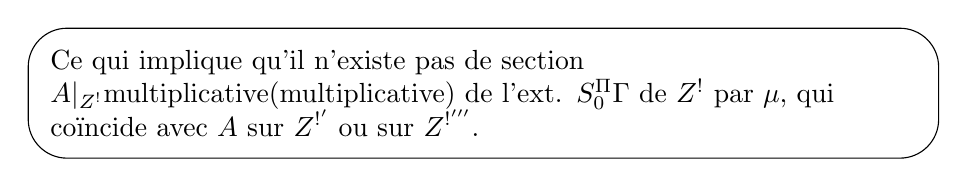
\begin{tikzpicture}
\node[draw,rounded corners=14pt,inner sep=8pt,text width=11cm,align=left]
{Ce qui \unsure{implique} qu'il n'existe pas de section
\deleted{$\unsure{A|_{Z^!}}$\unsure{multiplicative}}\inserted{(multiplicative)}
de l'ext. $S_0^{\Pi}\Gamma$ de $Z^!$ par $\mu$, qui coïncide
avec $A$ sur $Z^{!'}$ ou sur $Z^{!'''}$.};
\end{tikzpicture}}}

On a alors ceci:

a) $S_0^{\Pi_0}\Gamma^{!'},S_0^{\Pi_0}\Gamma^{!'''}$ ne sont
\uline{pas} \uline{distingués} dans $S_0^{\Pi}\Gamma^!$.

b) $S_0^{\Pi_0}\Gamma^{!0}$ est distingué dans
$S_0^{\Pi}\Gamma^!$, de sorte que l'ext.
$S_0^{\Pi}\Gamma^!$ de $Z^!\simeq M^![0]$ par $\mu$
est canoniquement isom. à l'image inverse d'une
\unsure{extension|catégorie} \inserted{centrale} finie
$S_0^{\Pi}\Gamma^!/(S_0^{\Pi_0}\Gamma^{!0})$
de $Z^!/Z^{!0}\simeq\mu\times\mu$ par $\mu$.

\mspage{599}
\scanpage{601}
\mspage{604}

Examinons cette extension centrale
\[
(84)\qquad
\diagram{\begin{tikzcd}[ampersand replacement=\&,column sep=large,row sep=small]
1\arrow[r]\&\mu\arrow[r]\&
\mathcal E\arrow[r,"{(\varepsilon_3,\varepsilon_2)}"]
\arrow[d,phantom,"{\rotatebox{90}{$\simeq$}}" description]\&
\mu\times\mu\arrow[r]\&1\\
\&\&S_0^\Pi\Gamma_{\rho,\sigma}/S_0^{\Pi_0}\Gamma^0_{\rho,\sigma}\&\&
\end{tikzcd}}
\]
s'insérant dans le diagramme d'extensions,
\[
(85)\qquad
\diagram{\begin{tikzcd}[ampersand replacement=\&,column sep=large,row sep=large]
1\arrow[r,dash]\&\mu\arrow[r]\&
\mathcal E\arrow[r,dash]\&\mu\times\mu\arrow[r,dash]\&1\\
1\arrow[r,dash]\&\mu\arrow[r]\arrow[u,"1"']\arrow[d,hook]\&
S_0^\Pi\Gamma^!_{\rho,\sigma}\arrow[r]\arrow[u]\arrow[d,hook]\&
Z^!_{\rho,\sigma}\arrow[u,"{(\varepsilon_3,\varepsilon_2)}"']
\arrow[d,leftrightarrow,"1"]\arrow[r,phantom,"{\simeq M[0]}" description]\&\vphantom{1}\\
1\arrow[r]\&L_\rho\times L_\sigma\arrow[r]\&
S_0\Gamma^!_{\rho,\sigma}\arrow[r]\&Z^!_{\rho,\sigma}\arrow[r]\&1
\end{tikzcd}}
\]

L'intérêt de (84) est qu'elle permet de récupérer l'extension
$S_0\Gamma_{\rho,\sigma}$ de $Z^!_{\rho,\sigma}$ par
$L_\rho\times L_\sigma$, par la \unsure{loi}
\unsure{covariante}-\unsure{contravariante} dans le foncteur
``extensions'', de
\[
(86)\qquad
\diagram{\begin{tikzcd}[ampersand replacement=\&,column sep=large,row sep=small]
Z^!_{\rho,\sigma}\arrow[r,"{(\varepsilon_3,\varepsilon_2)}"]\&
\mu\times\mu
\end{tikzcd}},\qquad
\begin{gathered}
\diagram{\begin{tikzcd}[ampersand replacement=\&,column sep=large,row sep=small]
\mu\arrow[r,hook]\&L_\rho\times L_\sigma\\
-1\arrow[r,mapsto]\&(\rho^3,\sigma^2)
\end{tikzcd}}\\
\text{(``hom. diagonal'')}
\end{gathered},
\]
ainsi que la sous-extension $S_0^\Pi\Gamma^!_{\rho,\sigma}$ de
celle-ci (de $Z^!_{\rho,\sigma}$ par $\mu$).

Étudions d'abord l'ordre des éléments de $\mathcal E$ --- ils sont
évidemment diviseurs de $4$, sont ils tous d'ordre $2$ (ou $1$)? Soit
\[
\underline{\unsure{\bar u|u}}=
\left(
\underset{\inserted{\substack{\rotatebox{90}{$\in$}\\Z}}}{u},
\underset{\inserted{\substack{\rotatebox{90}{$\in$}\\N_\rho^*}}}{a},
\underset{\inserted{\substack{\rotatebox{90}{$\in$}\\N_\sigma^*}}}{b}
\right)\in S_0^\Pi\Gamma^!
\qquad\text{i.e.}\quad
\left\{\begin{aligned}
u&\equiv b\quad(\widehat\Pi_0)\\
u&\equiv\varepsilon_3[\sigma]a\quad(\widehat\Pi)
\end{aligned}\right.
\qquad(87)
\]
\margin{\uline{NB} Pour \unsure{interdire|introduire} des confusions,
\unsure{j'écris} $\varepsilon_3[\sigma],\varepsilon_3[\tau']$
de préférence \unsure{à|de} $\varepsilon_3(\sigma),\varepsilon_3(\tau')$
pour $\sigma^{\unsure{\nu_3}},\tau'^{\unsure{\nu_3}}$.}

Je \deleted{\unsure{veux}} veux examiner si
$\underline{u}^{2}\in S_0^{\Pi_0}\Gamma^{!0}$.
Évidemment
\[
\underline{u}=(u^2,a^2,b^2)\in S_0^\Pi\Gamma^{!0}
\]

\mspage{600}
\scanpage{602}

il reste à voir si $\underline u^{2}\in S_0^{\Pi_0}\Gamma^{!}$, i.e. si on a
\deleted{\unsure{non}} seulement
$\unsure{u^{2}}\equiv b^{2}\ (\Pi_0)$ et
$\deleted{\unsure{a^{2}}}\unsure{u^{2}}\equiv a^{2}\ (\widehat\Pi)$
--- ce qui est clair et exprime simplement
$\underline u^{2}\in S_0^{\Pi}\unsure{\Gamma|\Gamma^{!}}$ --- mais même
\[
\tag{88}
\unsure{u^{2}}\equiv a^{2}\quad\bmod\ \uuline{\widehat\Pi_0}
\qquad (?)
\]

La relation
\[
u\equiv\varepsilon_3[\sigma].a\quad\bmod\Pi
\]
s'écrit aussi
\[
u\equiv\pm\varepsilon_3[\sigma].a\quad\bmod\Pi_0
\]
et implique
\[
u^2\equiv\varepsilon_3[\sigma]a\ \varepsilon_3[\sigma]a
\quad\bmod\Pi_0
\]
ce qu'on peut écrire
\[
\tag{89}
\underset{\bmod\widehat\Pi_0}{u^2\equiv
\varepsilon_3\,\varepsilon_3[\sigma](a).a}
=\begin{cases}
a^2&\text{si }\varepsilon_3=1.\\
-\sigma(a).a&\text{si }\varepsilon_3=-1
\end{cases}
\]

Donc (88) est vraie si $\varepsilon_3=1$, tandis que
pour $\varepsilon_3=-1$, elle équivaut à
\[
\sigma(a)\equiv-a\qquad(\widehat\Pi_0)
\]
i.e.
\[
[\sigma,a]^{\cdot}=-1\quad\text{dans }\unsure{\widetilde{\mathcal G}|\widetilde{\mathcal C}}/\Pi_0
\]
i.e.
\[
\underbrace{\varepsilon_2(a)}_{\inserted{\begin{gathered}\rotatebox{90}{$=$}\\\varepsilon_2(u)\end{gathered}}}=-1
\qquad\text{i.e. }\varepsilon_2(\unsure{u})\varepsilon_3(\unsure{u})=1.
\]

Donc on trouve :

\uline{Proposition} Soit $x\in\mathcal E$ (cf (84)). Pour que
l'on ait $x^2=1$, il f. et s. qu'on ait
$\varepsilon_3(x)=1$ \uline{ou} $\varepsilon_2(x)\varepsilon_3(x)=1$,
i.e. que
\deleted{$x$ \unsure{appartienne au sous-groupe} $\mathcal E'$ \unsure{ou}}
\inserted{l'on ait}
\[
\tag{90}
x\in\mathcal E'\cup\mathcal E''',
\]

\mspage{601}
\scanpage{603}
\mspage{605}

où
\[
\tag{91}
\mathcal E'=\{\unsure{x|n}\in\mathcal E\mid\varepsilon_3(x)=1\},\qquad
\mathcal E'''=\{\unsure{x|n}\in\mathcal E\mid\varepsilon_2(x)\varepsilon_3(x)=1\}
\]

\uline{Corollaire 1} $\mathcal E$ a exactement deux éléments
d'ordre $4$, qui sont les deux éléments de $\mathcal E$ au
dessus de l'élément $(-1,1)$ de $\mu\times\mu$.
Ces deux éléments sont inverses l'un de
l'autre, \unsure{ce|et} sont les deux générateurs du
seul sous-groupe cyclique d'ordre $4$ de $\mathcal E$,
qui n'est autre que
\[
\tag{92}
\mathcal E''=\{\unsure{x|n}\in\mathcal E\mid\varepsilon_2(x)=1\}
\]

\uline{Corollaire 2} L'extension $\mathcal E$ n'est pas scindée.

Car étant centrale, elle \deleted{\unsure{se}} serait isomorphe
à $(\mu\times\mu)\times\mu$, donc ses éléments seraient d'ordre
qui divise $2$.

Nous pouvons regarder maintenant
$\mathcal E$ comme extension de $\mathcal E/\mathcal E''\simeq\{\pm1\}=\mu$ par
$\mathcal E''\ (\simeq\mathbb Z/4\mathbb Z)$.
\deleted{Mais il} Il faudrait
d'abord expliciter l'opération de $\mathcal E/\mathcal E''=\mu$
sur $\unsure{\mathcal E'|\mathcal E''}$ --- l'élément \inserted{$-1$} d'ordre $2$ de $\mu$
induit un \unsure{autom.} involutif de \deleted{$\unsure{\mathbb Z/4\mathbb Z}$} $\mathcal E''$
\inserted{d'ailleurs dans $\mathrm{Aut}(\unsure{\mathcal E'|\mathcal E''})\simeq
(\mathbb Z/4\mathbb Z)^*\simeq\{\pm1\}$, donc
l'autom. en question}
\deleted{que \unsure{son}} est la multiplication par un
signe $\varepsilon\ \pm1$, qu'il faut déterminer. On va
prendre \inserted{comme représentant de $-1\in\mathcal E/\mathcal E''$}
l'élément de $\mathcal E$ provenant
\deleted{de}\inserted{de}
\[
\tag{92}
\deleted{\unsure{\tau,a',\tau}}\quad
\underline x=(u_0=\tau,\ a_0=\tau',\ b_0=\tau)
\in S_0^{\Pi_0}\Gamma^{!'''}\qquad(\text{cf}(70))
\]
qu'on va faire opérer sur l'image d'un
\[
\tag{93}
\underline u=(u,a,b)\in S_0^{\Pi}\Gamma^{!},\quad
\deleted{\unsure{\text{où}}}\ \text{avec }\varepsilon_3(u)=-1,\ \varepsilon_2(u)=1
\]
\inserted{\[
\left(\begin{array}{ll}
u\equiv b\ \deleted{\unsure{\equiv a}}&\bmod\widehat\Pi_0\\
u\equiv\sigma a&\bmod\widehat\Pi
\end{array}\right)
\]}
(qui est un générateur de $\mathcal E''$).

\mspage{602}
\scanpage{604}

On aura donc
\[
\underline x(\underline u)=(\tau(u),\tau'(a),\tau(b))\equiv
\deleted{\unsure{(u,\varepsilon a,\varepsilon b)|(\varepsilon u,\varepsilon a,\varepsilon b)}}
\underbrace{\inserted{(1,\varepsilon,\varepsilon)(u,a,b)}}_{\inserted{(u,\varepsilon a,\varepsilon b)}}
\]
mod $S_0^{\Pi_0}\Gamma^{\unsure{!0|0}}$, avec un signe
$\varepsilon\in\{\pm1\}$ à déterminer. La condition de congruence s'écrit
\[
(u\tau(u)^{-1},\ \varepsilon a\tau'(a)^{-1},\
\varepsilon b\unsure{\tau'(b)|\tau(b)}^{-1})\in S_0^{\Pi_0}\Gamma^{\unsure{!0|0}}
\]
qu'on soit dans $S_0^\Pi\Gamma^{!0}$ est évident,
\deleted{\unsure{le choix}}
\deleted{\unsure{indifférent|indépendant}}
\inserted{\unsure{valble|valable}}
quel que soit le choix du signe
$\varepsilon$, \deleted{\unsure{c'est}}
\deleted{\unsure{c'est|et}}\inserted{\unsure{c'est}}
\unsure{la|les} \unsure{condition|conditions} de congruence
\deleted{qui} \deleted{\unsure{sont essentielles}}
\inserted{qui \unsure{distingue|distinguent} $S_0^{\Pi_0}\Gamma^{!}$ de
$S_0^\Pi\Gamma^{!}$ qui est}
essentielle, savoir
\[
\tag{94}
u\tau(u)^{-1}\equiv\varepsilon\unsure{a}\tau'(\unsure{a})^{-1}
\qquad(\widehat\Pi_0)\qquad\text{soit}
\]
\deleted{\[
\unsure{u(\tau)\tau^{-1}\equiv\varepsilon a(\tau')\tau'^{-1}}
\]}

La difficulté avec cette approche vient
du fait que les seuls éléments de
$M$ qu'on sache expliciter sont ceux qui
proviennent de $\unsure{\widetilde{\mathcal G}|\widetilde{\mathcal C}}\simeq\mathrm{Gl}(2,\mathbb Z)$
lui-$\overline{\mathrm m}$ ; or
pour ceux-ci on a $\varepsilon_2(u)\varepsilon_3(u)=1$, alors
que le $u$-\inserted{ici} \deleted{\unsure{test}} ci-dessus doit satisfaire
$\varepsilon_2(u)=1$, $\varepsilon_3(u)=-1$ donc
$\varepsilon_2(u)\varepsilon_3(u)=-1$.
On \unsure{peut} d'autre part travailler dans le
\deleted{\unsure{\text{groupe}} $\unsure{\widetilde{\mathcal G}|\widetilde{\mathcal C}}$}
\inserted{quotient} $\mathrm{Gl}(2,\widehat{\mathbb Z})$ de
\deleted{$\unsure{\widetilde{\mathcal G}|\widetilde{\mathcal C}}$} $M$, et
y prendre
\[
\tag{95}
u=\begin{pmatrix}\mu&0\\0&1\end{pmatrix}
\quad\text{avec}\quad
\mu\in\widehat{\mathbb Z}^{*},\quad
\begin{cases}
\mu\equiv-1&(3)\\
\mu\equiv1&(4)
\end{cases}
\]
\inserted{\[\text{i.e.}\quad\mu\equiv5\quad(12)\]}
tandis que $\tau$ correspond à la
matrice
\[
\tau=\begin{pmatrix}-1&0\\0&1\end{pmatrix}
\]

\margin{$\unsure{\wedge}$}
\mspage{603}
\scanpage{605}
\mspage{606}

on aura de toutes façons
\[
u\tau(u)^{-1}=1
\]
soit d'autre part dans $\mathrm{Gl}(2,\widehat{\mathbb Z})$
\[
\tag{96}
\left\{\begin{array}{lll}
a=\tau'a_0&a_0=c\rho+d&c^2+cd+d^2\in\widehat{\mathbb Z}^{*}\\[3pt]
&\tau'=\begin{pmatrix}0&1\\1&0\end{pmatrix},&
\rho=\begin{pmatrix}0&1\\-1&1\end{pmatrix}
\end{array}\right.
\]
\unsure{donc|d'où}
\[
\tag{97}
a=\begin{pmatrix}0&1\\1&0\end{pmatrix}
\begin{pmatrix}d&c\\-c&c+d\end{pmatrix}
=\begin{pmatrix}-c&c+d\\d&c\end{pmatrix}
\]
et
\[
\tag{98}
\mu=-(c^2+cd+d^2)
\]

\margin{\unsure{un peu bref}... cf plus bas...}

On \deleted{\unsure{va}} travailler avec le \inserted{sous-}groupe fermé
$\widehat\Pi_0$ dans $\mathrm{Sl}(2,\widehat{\mathbb Z})$ engendré par
\[
\begin{gathered}
-\ell_0\underset{\unsure{,}}{\unsure{=}}\unsure{-}\begin{pmatrix}
1&-2\\\deleted{\unsure{-2|2}}0&1
\end{pmatrix},\qquad
-\ell_1=-\begin{pmatrix}1&0\\2&1\end{pmatrix},\qquad
-\ell_\infty=-\begin{pmatrix}3&-2\\2&-1\end{pmatrix}
\end{gathered}
\]
et dans le groupe quotient de
$\mathrm{Gl}(2,\widehat{\mathbb Z})$ par $\widehat\Pi_0$, qui est
\deleted{\unsure{l'}} l'extension de
$\widehat{\mathbb Z}^{*}$ par
\[
\mathrm{Sl}(2,\widehat{\mathbb Z})/\widehat\Pi_0
\simeq\mathrm{Sl}(2,\mathbb Z)/\Pi_0
\simeq\left\{(\rho,\sigma)\ \left|\begin{array}{l}
\rho^6=\sigma^4=1\\
\rho^3=\sigma^2\\
\sigma(\rho)=\rho^{-1}
\end{array}\right.\right\},
\]
\deleted{\unsure{avec}} et \unsure{ce|en} produit $\frac12$ direct grâce à
\[
T_0=\left\{\begin{pmatrix}
\deleted{\unsure{\xi}}\unsure{\zeta|\xi}&0\\0&1
\end{pmatrix}\ \middle|\ \unsure{\zeta|\xi}\in\widehat{\mathbb Z}^{*}\right\}
\overset{\det}{\simeq}\widehat{\mathbb Z}^{*},
\]
opérant par l'intermédiaire de $\varepsilon_2(\unsure{\zeta|\xi})$
--- cf p. $593'$, $594$ --- formules (34)(35)(35 bis) ].
On \inserted{doit} supposer
\[
\tag{99}
\sigma a\equiv u\qquad(\widehat\Pi_{\unsure{0}})
\qquad\text{où }\sigma=\begin{pmatrix}0&-1\\1&0\end{pmatrix}
\]
donc
\[
\tag{100}
\sigma a=\begin{pmatrix}-d&-c\\-c&c+d\end{pmatrix}
\]

\mspage{604}
% ===== LM_C3-606-624: second pass, checked against the scans =====
\scanpage{606}

\deleted{\unsure{Pour avoir}} \inserted{La relation} (99),
\deleted{il \unsure{suffit} d'\unsure{avoir}} s'écrit
\[
\tag{102}
\left\{\begin{aligned}
\deleted{\det}\sigma a&\equiv u\quad
(\mathrm{SL}(2,\widehat{\mathbb Z}))\quad\text{i.e.}\quad
\det\sigma a=\det u\quad\text{i.e. (98)}\\
\sigma a&\equiv u\quad(\deleted{4}2)
\end{aligned}\right.
\]
\deleted{\unsure{i.e.}} et cette dernière congruence s'écrit
\[
\tag{103}
c\equiv0\quad(\deleted{4}2)\qquad d\equiv1\quad(\deleted{4}2)
\qquad
\left(-d\equiv\mu\quad(\deleted{\unsure{4}}2)\ \text{\unsure{en est une conséquence}}
\ \text{car }\mu\equiv1\equiv-1\quad(2)\right).
\]

NB On ne \unsure{peut avoir les} \deleted{\illegible{3} $\mu\equiv-1\ (4)$, car}
congruences \uline{mod 4}
$(\sigma a\equiv u\ (4)$, car on aurait
$\mu\unsure{\equiv}-d\equiv-1\ (4)$, ce qui est contraire à l'hypothèse
(95) $\mu\equiv1\ (4)$.

\deleted{Ainsi (102) est \unsure{trop fort}. Néanmoins, il \uline{faut}
(pour avoir (99)) qu'on ait
\[
\tag{102 bis}
\sigma a\equiv u\quad(2)\qquad\text{i.e.}
\]
\[
\tag{103 bis}
c\equiv0\quad(2),\qquad d\equiv1\quad(2)
\]
(la relation $-d\equiv\mu\ (2)$ en est une conséquence, car
$\mu\equiv1\equiv-1\ (2)$). \unsure{Ce}}

Revenant à la relation (99), on trouve ceci :

\deleted{\uuline{Proposition}} \inserted{Lemme.} Soient
$c,d\in\widehat{\mathbb Z}^{\deleted{\unsure{*}}}$ satisfaisant
\[
\tag{104}
\mu\overset{\mathrm{dfn}}{=}-(c^2+cd+d^2)\in\widehat{\mathbb Z}^{*}
\]
\margin{\uline{NB} On aura néc.\textsuperscript{t} $\mu\equiv-1\ (3)$}
\[
\tag{105}
\mu\equiv1\quad(4)\qquad
(\text{i.e. }c^2+cd+d^2\equiv-1\quad(4)).
\]
\[
\tag{106}
c\equiv0\quad(2),\qquad d\equiv1\quad(2)
\]
Soit \deleted{\unsure{a c|a=}} \inserted{\unsure{d}}
\[
\tag{107}
a=\tau'(c\rho+d)=
\begin{pmatrix}-c&c+d\\d&c\end{pmatrix}
\in\mathrm{GL}(2,\widehat{\mathbb Z})
\]
(matrice de déterminant $\mu$). Alors on a une congruence
\[
\tag{108}
a\tau'(a)^{-1}\equiv\varepsilon\qquad
\mathrm{mod}\ \widehat{\Pi}_0\subset\mathrm{GL}(2,\widehat{\mathbb Z})
\]
\deleted{\unsure{et}} le signe $\varepsilon\in\{\pm1\}$ ne dépend pas des
choix faits pour $c,d$.
\scanpage{607}
\mspage{607}

C'est le moment de le calculer ! Reprenant
\[
a_0=c\rho+d\quad\in Z_\rho
\]
on aura
\[
a=\tau'a_0,\quad \tau'(a)=a_0\tau',\quad
a\tau'(a)^{-1}=\tau'a_0\tau'^{-1}a_0^{-1}=\tau'(a_0)a_0^{-1}
\]
où
\[
\left\{\begin{aligned}
\tau'(a_0)&=c\rho^{-1}+d={}^{t}a_0\\
a_0^{-1}&={}^{t}a_0/\det a_0=-\frac1\mu(c\rho^{-1}+d)
\end{aligned}\right.
\]
\margin{On \unsure{pose} \inserted{pour
$\unsure{u\in}\mathrm{M}_2(\widehat{\mathbb Z})$}
${}^{t}u=(\mathrm{Tr}\,u)-u$ et on a ${}^{t}\rho=\rho^{-1}$
(plus généralement ${}^{t}u=u^{-1}$ si $\det u=1$)}
donc
\[
a\tau'(a)^{-1}=\tau'(a_0)a_0^{-1}
=-\frac1\mu(c\rho^{-1}+d)^2
=\frac1{c^2+cd+d^2}(c\rho^{-1}+d)^2
\]
Or on a
\[
(c\rho^{-1}+d)^2
=c^2\underbrace{\rho^{-2}}_{-\rho}
+2cd\underbrace{\rho^{-1}}_{1-\rho}+d^2
=-(c^2+2cd)\rho+(2cd+d^2).
\]
Or \deleted{comme}
\[
\begin{aligned}
c\equiv0\quad(2)&\Longrightarrow c^2,2cd\equiv0\quad(4)
\qquad\text{\deleted{donc}}\\
d\equiv1\quad(2)&\Longrightarrow d^2\equiv1\quad(4)
\qquad\text{donc}
\end{aligned}
\]
\deleted{
\[
a\tau'(a)^{-1}\equiv\unsure{\pm}1\quad(4)
\qquad\text{\unsure{a fortiori a}}
\]
}
\[
(\unsure{*})\qquad (c\rho^{-1}+d)^2\equiv1\quad(4)
\]
\deleted{d'autre part.}

\deleted{donc le signe $\varepsilon$ est égal à \uline{$+1$}.}

Et comme par hypothèse
\[
c^2+cd+d^2\equiv-1\quad(4)
\]
on aura
\[
\tag{109}
a\tau'(a)^{-1}=\frac1{c^2+cd+d^2}(c\rho^{-1}+d)^{\unsure{2}}
\equiv-1\quad(4)
\]
Donc on a prouvé, en fait

\uline{Proposition} Soient $c,d\in\unsure{\mathbb Z|\widehat{\mathbb Z}}$
tels que $\xi\overset{\mathrm{dfn}}{=}c^2+\unsure{cd}+d^2
\in\widehat{\mathbb Z}^{*}$, soit
\[
a=\tau'(c\rho+d)=\begin{pmatrix}-c&c+d\\d&c\end{pmatrix}
\in\mathrm{GL}(2,\widehat{\mathbb Z}),
\]
\deleted{\unsure{démontrons|supposons}}
\[
\deleted{(\unsure{110})}\qquad
\deleted{a\tau'(a)^{-1}}\inserted{\sigma a}
\equiv\begin{pmatrix}\xi&0\\0&1\end{pmatrix}
\quad(2)\qquad\text{i.e.}
\]
\figure{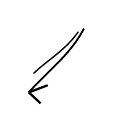
\begin{tikzpicture}[baseline]
\draw[line width=.65pt] (.8,.95) .. controls (.63,.62) and (.36,.43) .. (.1,.14);
\draw[line width=.8pt] (.1,.14)--(.34,.23) (.1,.14)--(.25,0);
\draw[line width=.5pt] (.73,.91) .. controls (.56,.67) and (.35,.56) .. (.16,.38);
\end{tikzpicture}}
\margin{\uline{NB} $\sigma=\begin{pmatrix}0&-1\\1&0\end{pmatrix}$}
\[
c\equiv0\quad(2),\qquad d\equiv1\quad(2).
\]
\scanpage{608}

Alors on a (pour $\tau'=\begin{pmatrix}-1&0\\0&1\end{pmatrix}$)
\[
a\tau'(a)^{-1}\equiv\varepsilon_2(\xi)\quad(4)
\]
(a fortiori on a la congruence mod $\widehat{\Pi}_0$).

\uline{Corollaire} L'extension $\mathcal E$ de $\mu\times\mu$ par $\mu$
(\unsure{84|89}), ou de $\mu$ par $\mathcal E''\simeq\mathbb Z/4\mathbb Z$, est non
commutative.
\margin{$\big|$}

Mais voici une façon de le voir sans calcul. Si l'extension était commutative,
\deleted{elle} \inserted{sa classe d'isomorphie} serait donnée par un
$\unsure{\mathrm{Ext}_{\mathbb Z}|\mathrm{Ext}^1_{\mathbb Z}}$
(ou un $\mathrm{Ext}^{\unsure{1|?}}_{\mathbb Z/4\mathbb Z}$).
Or le foncteur $\unsure{\mathrm{Ext}|\mathrm{Ext}^1}(-,\mu)$ est additif. Comme la restriction de
l'extension aux ss-groupes $\mathcal E'/\mu$ et $\mathcal E'''/\mu$ de
$\mu\times\mu$ est trivial, et que $\mu\times\mu$ est
la somme directe de ces sous-groupes (qui sont resp. $1\times\mu$ et le
sous-groupe diagonal), il s'ensuivrait que l'extension serait
trivial, or on a vu que ce n'est pas le cas.

\deleted{\unsure{En|Et}} \unsure{La} structure du groupe $\mathcal E$
s'explicite aisément, p.ex. en \unsure{tant} qu'extension de
$\mathcal E/\mathcal E''\simeq\mu$ par
$\mathcal E''\simeq\mathbb Z/4\mathbb Z$. \deleted{Soit}
Choisissons un élément quelconque de $\mathcal E-\mathcal E''$, il est
d'ordre 2 (les seuls élémts d'ordre 4 étant dans $\mathcal E''$) de sorte
que l'on a
\scanpage{609}
\mspage{608}

\[
\tag{110}
\mathcal E\simeq\{1,x\}\mathbin{.}\mathcal E''
\qquad\left(\tfrac12\ \text{direct}\right)
\]
Notons que si $x$ opérait trivialement sur $\mathcal E''$,
\deleted{i.e.} si $\mathcal E$ était isomorphe au produit, alors pour un
élément \inserted{$u$ de $\mathcal E''$} d'ordre 4,
$x.u$ serait d'ordre \unsure{4|8}, ce qui est absurde (troisième démonstration du fait
que \inserted{$\mathcal E/\mathcal E''\simeq$} $\mu$ opère non-trivialement
sur $\mathcal E''$). Or du seul fait que l'op. de $\{1,x\}$ sur
$\mathcal E''$ est non triv\unsure{.}, elle est connue, et
\inserted{la structure de} $\mathcal E$ est déterminée -- en fait on a
\[
\tag{\unsure{111|110}}
\mathcal E\simeq\mathbb D_4
\]
Il y a un choix privilégié de $x$, en prenant pour $x$ l'élém\unsure{t}
\[
\tag{112}
\left\{\begin{aligned}
\tau_{\mathcal E}&\overset{\mathrm{dfn}}{=}
\tau_{\unsure{S_0\Gamma}}\ \mathrm{mod}\ S_0^{\Pi}\Gamma^0,
\quad\text{où bien sûr}\\
\tau_{S_0\Gamma}&=(\tau,\tau',\tau),
\end{aligned}\right.
\]
de sorte que l'on a une représentation canonique
\[
\tag{113}
\mathcal E\simeq\{1,\tau_{\mathcal E}\}\mathbin{.}
\mathcal E''
\qquad\text{produit }\tfrac12\text{ direct}
\]
\margin{$\mathcal E''\simeq\mathbb Z/4\mathbb Z$\quad
$\tau_{\mathcal E}(u)=u^{-1}$ pour $u\in\mathcal E''$.}

L'hom $\mathcal E\to\mu\times\mu$ se récupère par ses restrictions aux
deux facteurs
\[
\tag{114}
\diagram{\begin{tikzcd}[column sep=large,row sep=large]
\mu\simeq\{1,\tau_{\mathcal E}\}\arrow[r]&\mu\times\mu&
\tau_{\mathcal E}\arrow[r,mapsto]&(-1,-1)\quad\text{(hom diagonal)}\\
\mathcal E''\arrow[r]&\unsure{\mu\times\{1\}}\arrow[r,hook]&\mu\times\mu&
\end{tikzcd}}
\]
l'unique hom non trivial $\mathcal E''\to\mu$ déduit de l'isom
\[
\diagram{\begin{tikzcd}
\mathcal E''_2\overset{\mathrm{dfn}}{=}
\unsure{\mathcal E''/2\mathcal E''|\mathcal E''/{}_{2}\mathcal E''}
\arrow[r,"\sim"]&\mu
\end{tikzcd}}
\]
\scanpage{610}

Le fait que $\mathcal E$ ne soit pas commutative s'exprime aussi par le fait
que l'hom can
\[
\tag{115}
\diagram{\begin{tikzcd}
\mathcal E_{\mathrm{ab}}\arrow[r,"\sim"]&\mu\times\mu
\end{tikzcd}}
\]
est un iso, i.e. que le sous-groupe noyau $\mu$ de
$\unsure{\mathcal E_{\mathrm{ab}}|\mathcal E}\to\mu\times\mu$ est aussi
le sous-groupe des commutateurs.

On a vu que l'extension $\mathcal E$ de $\mu\times\mu$ par $\mu$ n'est pas
scindée, mais qu'en est-il de son image inverse, l'extension
$S_0^{\Pi}\Gamma^!$ de $Z^!\simeq\mathcal M[0]$ par $\mu$ ? A priori,
on sait seulement qu'il n'y a pas de scindage de cette extension qui
prolonge le scindage canonique $A$ dont on dispose au dessus de
\[
Z^0=\mathrm{Ker}\left(\diagram{\begin{tikzcd}
Z^!\arrow[r,"(\varepsilon_3,\varepsilon_2)"]&\mu\times\mu
\end{tikzcd}}\right).
\]
Je présume que $\overline{\mathrm m}$ $S_0^{\Pi}\Gamma''$, extension de
$Z^{!\unsure{\prime\prime}}$ par $\mu$, est non triviale, et
$\overline{\mathrm m}$ l'extension qu'elle induit au sous-groupe
\[
\Gamma'_{\mathbb Q}=\Gamma_{\mathbb Q}\cap
\underbrace{\Gamma_{\mathbb Q}^{\prime\sim}}_{\substack{\wr\\\mathcal M(0)'}}
\subset\mathcal M^{\unsure{\xi|*}}(0)\subset\mathcal M^![0]=Z^!.
\]
Il serait intéressant d'identifier, \deleted{l'ext}
plus précisément, l'extension sur $\Gamma_{\mathbb Q}$, qu'elle induit, qui
correspond à un élément canonique
\[
\tag{115}
c\in H^{\unsure{2}}(\mathrm{Spec}\,\mathbb Q,\mu_2)\subset\mathrm{Br}(\mathbb Q)
\]
\scanpage{611}
\mspage{609}

Sauf erreur on aura
\[
\tag{115}
c=\underset{\text{(cup-produit)}}{\xi'\xi''},
\quad\text{où}\quad
\xi',\xi''\in
H^2(\mathbb Q,\unsure{\mu_2})
\]
sont les éléments qui décrivent respectivement les extensions
$\mathbb Q(\sqrt[3]{1})=\mathbb Q(\sqrt{-3})$, et
$\mathbb Q(\sqrt{3})$ --- contenues l'une et l'autre, ainsi que
$\mathbb Q(\sqrt{-1})=\mathbb Q(i)$, dans l'extension biquadratique
$\mathbb Q\bigl(\underset{\substack{\Vert\\\sqrt[2]{-1}}}{i},
\underset{\substack{\Vert\\\sqrt[3]{1}}}{j}\bigr)
=\mathbb Q(\sqrt[12]{1})$, le corps des racines
$12^{\text{ièmes}}$ de l'unité (dont le groupe de Galois est
$(\mathbb Z/12\mathbb Z)^*\simeq(\mathbb Z/3\mathbb Z)^*\times
(\mathbb Z/4\mathbb Z)^*\simeq\mu\times\mu$).

Il doit être trivial --- quand on \unsure{connaît} un peu les fondements ---
que $c$ ainsi explicité est $\ne0$, et n'est pas non plus
\unsure{scindé} en passant à $\mathbb Q(i)$, le troisième larron.

\figure{\begin{tikzpicture}\draw (0,0)--(2,0);\end{tikzpicture}}

Considérons maintenant le $\mu$-\unsure{groupement} central
\margin{\uline{NB} $Z\simeq\mathcal M[0]$, $\gamma\simeq\widetilde{\Gamma}_{\mathbb Q}$}
\[
\tag{116}
\diagram{\begin{tikzcd}[column sep=large]
\mu \arrow[r,hook,"i_{\rho,\mu}"] &
S_0\Gamma^!_{\rho,\sigma}
=Z^!_{\rho,\sigma}\times_\gamma N^*_\rho\times_\gamma N^*_\sigma\\
\varepsilon \arrow[r,mapsto] & (1,\varepsilon,1)
\end{tikzcd}}
\]
à valeurs dans
\[
\operatorname{Ker}(S_0\Gamma^!_{\rho,\sigma}\longrightarrow
Z^!_{\rho,\sigma})\simeq L_\rho\times L_\sigma,
\]
on a donc un hom. canonique de relèvement
\[
\tag{117}
\diagram{\begin{tikzcd}[column sep=large]
\mathcal M^![0]\simeq Z^!_{\rho,\sigma}
\simeq S_0^\Pi\Gamma^!_{\rho,\sigma}/\mu
\arrow[r] & S_0\Gamma^!_{\rho,\sigma}/i_{\rho,\mu}(\mu),
\end{tikzcd}}
\]
\scanpage{612}

qui s'explicite en termes \unsure{\deleted{des}|des} deux hom.
canoniques fondamentaux
\margin{Ceci mérite d'être explicité dans un théorème récapitulatif $\ldots$}
\[
\tag{118}
\diagram{\begin{tikzcd}[column sep=large,row sep=small]
Z^!_{\rho,\sigma} \arrow[r,"\uline{a}"]
\arrow[d,phantom,"\simeq"{description,sloped}] & N^*_\rho/\mu,
& Z^!_{\rho,\sigma} \arrow[r,"\uline{b}"] & N^*_\sigma\\
\mathcal M[0] \arrow[d,phantom,"\simeq"{description,sloped}] &&&\\
\widetilde{\Gamma}_{\mathbb Q}\mathbin{.}L_0^{\unsure{\Pi}} &&&
\end{tikzcd}}
\]
où, je rappelle
\[
\tag{119}
\left\{\begin{array}{l}
N^*_\rho\subset\mathcal M=\widetilde N_{1,1}\simeq
\widetilde\Gamma_{\mathbb Q}\mathbin{.}
\underbrace{\mathcal G^+}_{\mathrm{SL}(2,\mathbb Z)^\wedge}\\
\Vert\\
\{u\in\mathcal M\mid
u(\rho)=\deleted{\text{\unsure{fixe le gr.}}}\rho^{\varepsilon_3(u)}\}\\[1ex]
\deleted{\unsure{\{}}N^*_\sigma\subset\mathcal M\\
\Vert\\
\{u\in\mathcal M\mid u(\sigma)=\sigma^{\varepsilon_2(u)}
\ (=\varepsilon_2(u)\sigma)\}.
\end{array}\right.
\]

Les applications $\uline{a},\uline{b}$ sont données par les formules (cf 51)
\[
\tag{120}
\left\{\begin{array}{ll}
\uline{a}(u)=a=\varepsilon_3[\tau']\alpha^{-1}u,
& \uline{b}(u)=b=\beta^{-1}u\quad\text{i.e.}\\
\alpha=ua^{-1}\varepsilon_3[\tau'],&\beta=ub^{-1}
\end{array}\right.
\]
où $\alpha\in\widehat\Pi_{0\tau}$, $\beta\in\widehat\Pi_0$
sont caractérisés par
\[
\tag{121}
u(\rho)=\operatorname{int}(\alpha)(\rho),\quad
u(\sigma)=\varepsilon_2(\sigma)\operatorname{int}(\beta)(\sigma).
\]
Les quantités \deleted{\unsure{$a,$}}
$a=\uline{a}(u)\inserted{\in N^*_\rho/\mu}$,
$b=\uline{b}(u)\inserted{\in N^*_\sigma}$ sont caractérisées en termes de
$u\in Z^!$ (à un signe près seulement) par les congruences
\[
\tag{122}
u\equiv b\quad(\widehat\Pi_0),\qquad
u\equiv\varepsilon_3[\sigma]a\quad(\widehat\Pi),
\]
qui impliquent a fortiori (réduisant mod $\mathcal G^{+\wedge}$),
qu'on a commutativité \unsure{du|de},
\scanpage{613}
\mspage{\unsure{619|610}}

\deleted{(\unsure{123|122})}
\[
\tag{123}
\diagram{\begin{tikzcd}[column sep=large,row sep=small]
&N^*_\rho/\{\unsure{\pm}1\}\arrow[dr,"\delta_\rho"]&\\
Z^!_{\rho,\sigma}\arrow[ur]\arrow[dr]
\arrow[rr,dashed,"\delta_Z"]&&\gamma_{\rho,\sigma}\simeq\widetilde\Gamma_{\mathbb Q}\\
&N^*_\sigma\arrow[ur,"\delta_\sigma"']&
\end{tikzcd}}
\]

\deleted{Considérons maintenant les deux $\mu$-groupements}
\[
\deleted{(124)}\qquad
\diagram{\begin{tikzcd}[column sep=large]
\deleted{\mu}\arrow[r] &
\deleted{S_0\unsure{\mathcal M|\Gamma}_{\rho,\sigma}}
\end{tikzcd}}
\]

Il serait temps de rectifier la confusion (p.\ \unsure{594'}) entre
$Z=Z_{\rho,\sigma}\not\subset
\mathcal M_{0,3}^{\unsure{\circ|\bullet}\sim}$,
et $Z^!=Z^!_{\rho,\sigma}=\deleted{\unsure{\mathcal M}}
Z\cap\mathcal M_{0,3}^{!\sim}$.
On a en fait
\[
\tag{124}
\diagram{\begin{tikzcd}[column sep=small,row sep=large]
Z_{\rho,\sigma}^{\deleted{\unsure{!}}}\simeq
\underset{\frac12\text{-direct}}{\mathcal M^{\unsure{\xi}}(0)\mathbin{.}L_0^{\mathcal G}}
\subset\mathcal M\arrow[dr,"\sim"]&\\
&\mathcal M_{0,3}^{\unsure{\xi}\sim}(0)\mathbin{.}
L_0^{\mathcal G_{0,3}}\subset\widetilde{\mathcal M}_{0,3}
\end{tikzcd}}
\]
\[
\tag{125}
\diagram{\begin{tikzcd}[column sep=small,row sep=large]
Z^!_{\rho,\sigma}\simeq Z^!_{\rho,\sigma}\cap\mathcal M^!
=\underset{\frac12\text{-direct}}{\mathcal M(0)\mathbin{.}L_0^\Pi}
\subset\mathcal M\arrow[dr,"\sim"]&\\
&\widetilde{\mathcal M}_{0,3}(0)\mathbin{.}L_0^{\Pi_{0,3}}
\deleted{\unsure{\subset\widetilde{\mathcal M}_{0,3}}}
\inserted{(\subset\widetilde{\mathcal M}_{0,3})}
\end{tikzcd}}
\]

Le lien entre les deux est donné par le diagramme
\[
\tag{126}
\diagram{\begin{tikzcd}[column sep=small,row sep=large]
1\arrow[r]&L_0^\Pi\arrow[r]\arrow[d,hook]&
Z^!_{\rho,\sigma}\arrow[r]\arrow[d,hook]&
\gamma_{\rho,\sigma}\arrow[r]\arrow[d,equal]&1\\
1\arrow[r]&L_0^{\mathcal G}\arrow[r]&
Z_{\rho,\sigma}\arrow[r]&
\gamma_{\rho,\sigma}\arrow[r]
\arrow[d,phantom,"\simeq"{description,sloped}]&1\\
&&&\mathcal M(0)\simeq\widetilde\Gamma_{\mathbb Q}&
\end{tikzcd}}
\]
où $L_0^\Pi\longrightarrow L_0^{\mathcal G}$ est
l'inclusion d'indice $2$ de
\[
\tag{127}
\diagram{\begin{tikzcd}[column sep=large,row sep=small]
L_0^\Pi=\ell_0^{\widehat{\mathbb Z}}
\arrow[r,hook]\arrow[d,phantom,"="{description,sloped}]&
\deleted{\unsure{\ell_0^{\widehat{\mathbb Z}}|\varepsilon_0^{\widehat{\mathbb Z}}}}
L_0^{\mathcal G}=\varepsilon_0^{\widehat{\mathbb Z}}\\
\varepsilon_0^{2\widehat{\mathbb Z}}&
\end{tikzcd}}
\]
Bien entendu, c'est bien sur $Z^!_{\rho,\sigma}$, non sur
$Z_{\rho,\sigma}$, qu'on a défini (117), (118) d'où (123).
\scanpage{614}

Je m'intéresse à la restriction des hom (123) au sous-groupe
$L_0^\Pi$ de $Z^!_{\rho,\sigma}$
la caractérisation (122) montre que l'hom induit
\[
\diagram{\begin{tikzcd}[column sep=large]
L_0^\Pi\arrow[r]&N^*_\rho/\{\pm1\}
\end{tikzcd}}
\]
\deleted{est}
est trivial (car $a$ en termes de $u$ ne dépend que de $u$ mod
$\widehat\Pi$), tandis que l'hom induit
\[
\diagram{\begin{tikzcd}[column sep=large]
L_0^\Pi\arrow[r]&N^*_\sigma
\end{tikzcd}}
\]
se factorise par $L_0^\Pi/L_0^{\Pi_0}\simeq\mathbb Z/2\mathbb Z$
(car $b$ en termes de $u$ ne dépend que de $u$ mod $\widehat\Pi_0$).
Sa valeur \inserted{$b$} sur \deleted{$\varepsilon_0$} $\ell_0$ est
\deleted{donnée}\inserted{\unsure{caractérisée|caractérisé}}
par les conditions
\[
\unsure{\{}\qquad b\in N^*_\sigma,\qquad b\equiv\ell_0\quad(\Pi_0)
\]
qui sont satisfaites évidemment par $b=-1$. Donc
Il y a lieu d'introduire aussi, qu'on le veuille ou non, le
$\mu$-groupement central canonique
\[
\tag{128}
\diagram{\begin{tikzcd}[column sep=large]
\mu\arrow[r,hook]&N^*_\sigma\\
-1\arrow[r,mapsto]&-1
\end{tikzcd}}
\]
et on a commutativité de
\[
\tag{129}
\diagram{\begin{tikzcd}[column sep=large,row sep=large]
L_0^\Pi\arrow[r,hook]\arrow[d]&Z^!_{\rho,\sigma}\arrow[d]\\
L_0^\Pi/L_0^{\Pi_0}\simeq\mu\arrow[r,hook]&N^*_\sigma.
\end{tikzcd}}
\]
Donc on trouve, à partir des deux hom. (123),
\scanpage{615}
\mspage{611}

de $Z^!_{\rho,\sigma}$, par passage au quotient deux hom canoniques
\[
\tag{130}
\left\{
\diagram{\begin{tikzcd}[column sep=large,row sep=small]
\gamma_{\rho,\sigma}\arrow[r]\arrow[d,equal]&N^*_\rho/\{\pm1\}\\
\widetilde\Gamma_{\mathbb Q}\arrow[d,equal]&\\
\gamma_{\rho,\sigma}\arrow[r]&N^*_\sigma/\{\pm1\},
\end{tikzcd}}
\right.
\]
qui sont en fait des sections des
\[
\diagram{\begin{tikzcd}[column sep=large,row sep=small]
N^*_\rho/\{\pm1\}\arrow[r]&\gamma_{\rho,\sigma}\arrow[d,equal]&\\
&\widetilde\Gamma_{\mathbb Q}\arrow[d,equal]&\mathcal M(0)\arrow[l,"\sim"']\\
N^*_\sigma/\{\pm1\}\arrow[r]&\gamma_{\rho,\sigma},&
\end{tikzcd}}
\]
de sorte qu'on trouve des décompositions,
\[
\tag{131}
\left\{\begin{array}{l}
N^*_\rho/\pm1\simeq\gamma_{\rho,\sigma}
\deleted{\unsure{\ltimes|\times}}\mathbin{.}
\underbrace{SZ_\rho/\{\pm1\}}_{=L_\rho/\{\pm1\}\simeq\mathbb Z/3\mathbb Z}\\[2ex]
N^*_\sigma/\pm1\simeq\gamma_{\rho,\sigma}\mathbin{.}
\underbrace{SZ_\sigma/\pm1}_{=L_\sigma/\pm\ \simeq\mathbb Z/2\mathbb Z}
\end{array}\right.
\]
(produits $\frac12$-directs). L'opération de $\gamma_{\rho,\sigma}$ sur
$L_\rho/\{\pm1\}\simeq\mathbb Z/3\mathbb Z$ est donnée par le
caractère quadratique $\varepsilon_3$, celle sur
$L_\sigma/\{\pm1\}\simeq\mathbb Z/2\mathbb Z$ est donnée par le caractère
quadratique $\varepsilon_2$.

La symétrie de présentation des deux hom (130) est un peu
\unsure{bidon} --- p.ex. l'hom
$\widetilde\Gamma_{\mathbb Q}=\gamma_{\rho,\sigma}\longrightarrow
N^*_\sigma/\{\pm1\}$ se remonte de façon évidente en
\[
\tag{132}
\diagram{\begin{tikzcd}[column sep=small,row sep=large]
\widetilde\Gamma_{\mathbb Q}=\gamma_{\rho,\sigma}\arrow[rr]&&N^*_\sigma,&\\
&\mathcal M(0)\arrow[ul,"\sim"]
\arrow[rr,phantom,"\subset"{description}]&&\mathcal M[0]=Z^!\arrow[ul]
\end{tikzcd}}
\]
\scanpage{616}

Une autre façon de le voir est de noter que
\[
 (132)\qquad \gamma_{\rho,\sigma}\simeq
 \mathcal M_0^{\unsure{!}}[0]/L_0^{\Pi_0}
\]
où
\[
 \mathcal M_0^{\deleted{\unsure{*}}!}[0]
 \overset{\mathrm{dfn}}{=}
 \mathcal M_{\unsure{\delta|0}}(0).L_0^{\Pi_0}
 \underset{\substack{\text{ss-groupe}\\\text{d'indice }2}}{\subset}
 \mathcal M^![0]=\mathcal M(0).L_0^{\unsure{\Pi|\tau}}
\]

Or sur $L_0^{\Pi_0}$, l'hom induit par
\diagram{\begin{tikzcd}
 \mathcal M^![0]=Z^!_{\rho,\sigma} \arrow[r] & N^*_{\sigma}
\end{tikzcd}}
est trivial. Ainsi on a $\overline{\mathrm m}$ un
\deleted{\unsure{isomorphisme}} scindage de
\[
 (133)\qquad
 \diagram{\begin{tikzcd}[column sep=large]
 1 \arrow[r] & L_{\sigma} \arrow[r] & N^*_{\sigma} \arrow[r]
 & \gamma_{\rho,\sigma} \arrow[r] \arrow[d, phantom, "\simeq" {rotate=90}] & 1\\
 &&& \widetilde{\Gamma}_{\mathbb Q}
 \end{tikzcd}}
\]
en un produit $\frac12$-direct
\[
 \deleted{\unsure{(134)}}\qquad
 N^*_{\sigma}\simeq\gamma_{\rho,\sigma}.L_{\sigma}
\]
qu'il vaut mieux écrire en concrétisant le sous-groupe section en
\unsure{tant} que ss-groupe de $G_{\rho,\sigma}\simeq\mathcal M$, soit donc
\[
\begin{aligned}
 (134)\qquad
 \unsure{N}_{0\sigma}^{!*}
 &\overset{\mathrm{dfn}}{=}
 \operatorname{Im}(\mathcal M_0[0]\longrightarrow N^*_{\rho})\\
 &=\operatorname{Im}(\mathcal M[0]\hookrightarrow N^*_{\rho})\\
 &=\{\beta^{-1}u\mid u\in\mathcal M(0),\ \beta\in\widehat\Pi_0
       \text{ tels que }u(\sigma)=\varepsilon_{\unsure{2}}(u)
       \operatorname{int}(\beta)(\sigma)\}\\
 &=\{v\in N^*_{\sigma}\mid \exists\,\beta\in\widehat\Pi_0\text{ tel que }
       \beta v\in\mathcal M[0]=\operatorname{Norm}_{\mathcal M}(\unsure{l_0})
       \cap\mathcal M^!\}
\end{aligned}
\]
\margin{\uline{NB} On définit $\mathcal M^!$ comme l'image inverse de
$\mathcal M_{0,3}^{!\sim}$, i.e. le noyau de la représentation canonique
\diagram{\begin{tikzcd}
 \mathcal M \arrow[r] &
 \underbrace{\mathcal G^{+\wedge}/\Pi^{\wedge}}_{\mathcal G_3}
 \arrow[r,"\sim"] &
 \operatorname{Aut}(\mathcal G^{+\wedge}/\Pi^{\wedge})
\end{tikzcd}}}

Posant
\[
 (135)\qquad
 \mathcal M_0^!\overset{\mathrm{dfn}}{=}\mathcal M(0).\Pi_0
 \underset{\substack{\text{indice}\\2}}{\subset}
 \mathcal M^!\overset{\mathrm{dfn}}{=}\mathcal M(0).\Pi,
\]
\scanpage{617}
\mspage{612}

de sorte qu'on a
\[
 (136)\qquad \mathcal M^!\simeq\mathcal M_0^!\times\mu,
\]
\margin{\uline{NB} On a
\diagram{\begin{tikzcd}
 \mathcal M_0^!\arrow[r,"\sim"] & \mathcal M_{0,3}^{!\sim}
\end{tikzcd}}}
on a donc
\[
 (137)\qquad
 \left\{\begin{aligned}
 N_{\sigma0}^{\deleted{\unsure{d}}*!}&=N^*_{\sigma}\cap\mathcal M_0^!\\
 N_{\sigma}^{*!}&\overset{\mathrm{dfn}}{=}N^*_{\sigma}\cap\mathcal M^!
                    =N_{\sigma0}^{*!}\times\mu,
 \end{aligned}\right.
\]
et on trouve que
\[
 (138)\qquad
 \diagram{\begin{tikzcd}
 N_{\sigma0}^{\unsure{*!|d!}}\arrow[r,"\sim"] &
 \gamma_{\rho,\sigma}=\widetilde\Gamma_{\mathbb Q}
 \end{tikzcd}}
\]
\deleted{\unsure{d'où}} Posons pour abréger
\[
 \deleted{(139)\qquad N_{\sigma}^{\unsure{d}}\simeq N_{\sigma0}^{*!}}
\]
\[
 (139)\qquad \mathcal M(1/2)=N_{\sigma0}^{*!}\qquad\text{cf }(137)
\]
on aura donc que $\mathcal M(1/2)$ est \unsure{un|une}
\inserted{\unsure{groupe-}}section
\deleted{(140)} pour $N_{\sigma}^{\unsure{*|\wedge}}$ extension de
$\gamma_{\rho,\sigma}$ par $L_{\unsure{\sigma|\rho}}$, et a fortiori pour
$\mathcal M$ ext. de $\gamma_{\rho,\sigma}$ par $\mathcal G^{+\wedge}$,
et \unsure{un|on} $\unsure{\overline{\mathrm m}|\simeq}$ \unsure{de plus|simples} pour
$\mathcal M_0^!,\mathcal M^!$
\[
 (140)\qquad
 \left\{\begin{aligned}
 \mathcal M_0^!&\simeq\mathcal M(1/2).\widehat\Pi_0\\
 \mathcal M^!&\simeq\mathcal M(1/2).\widehat\Pi\\
 \mathcal M&\simeq\mathcal M(1/2).\mathcal G^{+\wedge}\\
 N^*_{\sigma}&\simeq\mathcal M(1/2).L_{\sigma}
 \end{aligned}\right.
\]
\margin{$\longleftarrow$ attention, $\mathcal M^!$ est inv. dans $\mathcal M$
et $\mathcal M_0^!$ est inv. dans $\mathcal M^!$, mais
\uline{non dans} $\mathcal M$\quad cf plus bas}

[Si on veut \unsure{paraphraser} en introduisant
\[
 (141)\qquad
 N_{\rho0}^{*!}\overset{\mathrm{dfn}}{=}N^*_{\rho}\cap\mathcal M_0^!
 =\{v\in N^*_{\rho}\mid\exists\,\alpha\in\widehat\Pi_0\text{ tel que }
       \underbrace{\alpha v}_{u}\in\mathcal M(0)\}
\]
c'est donc l'un des $v$ qu'on peut associer au
$u\in\mathcal M(0)\subset\mathcal M^![0]=Z^!_{\rho,\sigma}$,
à l'aide des $\alpha\in\Pi_0$ tel que
$\alpha^{-1}u\in N_{\rho}^{\unsure{*|\wedge}}$ i.e.
\[
 u(\rho)=\operatorname{int}(\alpha)(\rho^{\varepsilon_3})
 \qquad\text{où}\quad\varepsilon_3=\varepsilon_3(u)=\varepsilon_3(v).
\]
Mais comme $u(\rho)$ doit avoir $\overline{\mathrm m}$ image dans
$\mathcal G_3=\mathcal G^{+\wedge}/\Pi$
que $\rho$, il faut qu'on ait $\varepsilon_3=1$, et alors
$\alpha$ est l'élément $\uline{\alpha}(u)$ associé à $u$ et
$v=\alpha^{-1}u$ est l'image can. de $u$ dans $N^{!*}_{\rho}$. Ainsi on
\scanpage{618}

trouve

\uline{Proposition} L'hom
$N_{\rho0}^{*!}\longrightarrow\gamma_{\rho,\sigma}=\widetilde\Gamma_{\mathbb Q}$
est injectif, et a pour image
$\gamma'_{\rho,\sigma}=\{\gamma\in\gamma_{\rho,\sigma}\mid\varepsilon_3(\gamma)=1\}$.

\uline{Corollaire}
$N_{\rho,0}^{*!}\subset Z_{\rho}^{\unsure{\xi|*}!}$ i.e.
$N_{\rho0}^{*!}=\deleted{\unsure{N}}Z_{\unsure{0\rho|\rho0}}^{\unsure{\xi|*}!}
 \overset{\mathrm{dfn}}{=}Z_{\rho}^{\unsure{\xi|*}}\cap\mathcal M_0^!$.

Il est naturel de poser
\[
 (142)\qquad N_{\rho0}^{*!}=Z_{\rho0}^!=\mathcal M(-\bar j)\,\unsure{..|.}
\]
Comme $N_{\rho}^{*!}\supset Z_{\rho}^!\supset\mu$, on voit que l'on a
\[
 (142)\qquad
 \left\{\begin{array}{rcll}
 N_{\rho\deleted{\unsure{0}}}^{*!}&=&N_{\rho0}^{*!}\times\mu
     &\bigl(\text{donc }N_{\rho}^{*!}=Z_{\rho}^!\bigr)\\
 \Vert&&&\\[-1ex]
 Z_{\rho}^!&=&Z_{\rho\unsure{0}}^!\times\mu&
 \end{array}\right.
\]
\[
 \deleted{\unsure{N_{\rho}}\simeq}
\]

Le sous-groupe $Z^!_{0,\rho}=\mathcal M(-\bar j)$ est une section de
$\mathcal M'$ sur $\gamma'_{\rho,\sigma}\simeq\Gamma_{\mathbb Q}^{\prime\sim}$,
et \deleted{\unsure{est}} \inserted{\unsure{$\mathcal M'$}}
\unsure{contenue|contenu} dans
\deleted{$Z^!_{0\rho}$ a fortiori dans}
$\mathcal M_0^{\prime!},\mathcal M^{\prime!},
 \deleted{\unsure{Z_{0\rho}}},Z_{\rho}^!,Z_{\rho}$,
on aura des décompositions en produit $\frac12$ direct
\[
 (143)\qquad
 \left\{\begin{aligned}
 \mathcal M_0^{\prime!}&\simeq\mathcal M(-\bar j).\Pi_0\\
 \mathcal M^{\prime!}&\simeq\mathcal M(-\bar j).\Pi\\
 \mathcal M^{\prime\unsure{\xi|*}}&\simeq\mathcal M(-\bar j).\mathcal G\\
 Z_{\rho}^!&\simeq\deleted{Z}\mathcal M^{\unsure{\xi|*}}(-\bar j)\times\mu\\
 Z_{\rho}^{\unsure{\xi|*}}&\simeq\mathcal M^{\unsure{\xi|*}}(-\bar j)\times L_{\rho}
 \qquad ....
 \end{aligned}\right.
\]
]

\deleted{Notons maintenant que}
\[
 \deleted{\mu_{\tau'}\overset{\mathrm{dfn}}{=}\{1,\tau'\}\subset\mathcal G^{\wedge}}
\]
\deleted{normalise $L_{\rho}$, donc $Z_{\rho}$, donc
$Z^!_{0,\rho}=Z_{\rho}\cap\mathcal M_0^!$}
\scanpage{619}
\mspage{613}

Revenons au diagramme (130), je dis que l'hom
\diagram{\begin{tikzcd}
 \gamma_{\rho,\sigma}\arrow[r]\arrow[d,phantom,"\Vert"] & N^*_{\rho}/\{\pm1\}\\
 \Gamma_{\mathbb Q}^{\sim}
\end{tikzcd}}
\uline{ne se relève pas} en un hom de $\gamma_{\rho,\sigma}$ dans
$\underset{\inserted{\widetilde\gamma_{\rho,\sigma}}}{N^*_{\rho}}$
--- en d'autres termes, que l'extension de $\gamma_{\rho,\sigma}$ par
$\{\pm1\}=\mu$ qu'elle définit n'est pas triviale. Pour identifier cette
extension, considérons le diagramme
\margin{\uline{NB}}
\[
(144)\qquad
\diagram{\begin{tikzcd}[column sep=large,row sep=huge]
 \mathcal M^![0]=Z^!_{\rho,\sigma}\arrow[rr,"\text{can}"]
 &&\gamma_{\rho,\sigma}=Z^!_{\rho,\sigma}/L_0^{\Pi}
       \arrow[r,"\text{hom }(130)"]
 &N^*_{\rho}/\{\pm1\}\\
 S_0\Gamma^!_{\rho,\sigma}
       \arrow[u,"{\text{can}\quad(u,a,b)\mapsto u}"']
 &\inserted{\unsure{S_0}\Gamma_{\rho,\sigma}\quad\text{(sans !)}}
       \arrow[ur,very thick,"{\substack{\text{can}\\\unsure{\text{(passage au quotient)}}}}"']
 &&\\
 S_0^{\Pi}\Gamma^!_{\rho,\sigma}\arrow[u,hook,"\text{incl.}"']
       \arrow[ur,hook,dashed,"\text{incl.}"']\arrow[rrr]
 &&&N^*_{\rho}\arrow[uu]
\end{tikzcd}}
\]
qui montre que l'on a un diagramme de carrés cartésiens
\[
(145)\quad\deleted{\unsure{(146)|(144)}}\qquad
\diagram{\begin{tikzcd}[column sep=large,row sep=huge]
 \mathcal M(0)\arrow[r,hook]\arrow[dr,phantom,"\mathrm I" description]
 &\mathcal M^![0]=Z^!_{\rho,\sigma}\arrow[r,"\text{épi}"]
       \arrow[dr,phantom,"\mathrm {II}" description]
 &\gamma_{\rho,\sigma}\arrow[r,hook]
       \arrow[dr,phantom,"\mathrm {III}" description]
 &N^*_{\rho}/\{\pm1\}\\
 \mathcal M(0)^{\sim}\arrow[u]\arrow[r,hook]
 &S_0^{\Pi}\Gamma^!_{\rho,\sigma}\arrow[u,"2"]\arrow[r]
 &\widetilde\gamma_{\rho,\sigma}\arrow[u,"2"]\arrow[r,hook]
 &N_{\rho}^{\unsure{*|d}}\arrow[u,"2"]
\end{tikzcd}}
\]
où $\mathcal M(0)^{\sim}$ est \unsure{définie|défini} comme l'extension de
$\mathcal M(0)$ par $\mu$ induite par l'ext.
$S_0^{\Pi}\Gamma^!_{\rho,\sigma}$ de $\mathcal M^![0]$,
qui s'identifie donc \unsure{aussi} à l'image \unsure{réc.|réci.} de
\scanpage{620}

l'ext. $\widetilde\gamma_{\rho,\sigma}$ de $\gamma_{\rho,\sigma}$ par $\mu$,
par l'isom. composé
\diagram{\begin{tikzcd}
 \mathcal M(0)\arrow[r,"\sim"] & \gamma_{\rho,\sigma}.
\end{tikzcd}}
Donc l'ext. $\widetilde\gamma_{\rho,\sigma}$ de $\gamma_{\rho,\sigma}$ par
$\mu$ s'identifie \unsure{nt.|nat.} à l'ext. $\mathcal M(0)^{\sim}$ de
$\mathcal M(0)$ par $\mu$ dont on s'est convaincu plus ou moins qu'elle
n'était pas triviale.

Voici une autre façon d'obtenir l'hom canonique
\diagram{\begin{tikzcd}
 \gamma_{\rho,\sigma}\arrow[r] & N^*_{\rho}/\pm1,
\end{tikzcd}}
et l'extension $\widetilde\gamma_{\rho,\sigma}$ de $\gamma_{\rho,\sigma}$.
Considérons
\[
 (146)\qquad N_{\rho}^{*!}=N^*_{\rho}\cap\mathcal M^!
\]
On a alors
\[
 (147)\qquad
 N_{\rho}^{*!}\cap\mathcal G^+
 =\operatorname{Ker}\bigl(N_{\rho}^{*!}\longrightarrow
     \underbrace{\gamma_{\rho,\sigma}}_{\Gamma_{\mathbb Q}^{\unsure{\sim}}}\bigr)
 =L_{\rho}\cap\Pi=\mu
\]
d'autre part le hom
\[
 (148)\qquad
 \diagram{\begin{tikzcd}
 N_{\rho}^{*!}\arrow[r] & \gamma_{\rho,\sigma}
 \end{tikzcd}}
 \quad\text{est \uline{épi}}
\]
Car \deleted{pour $\forall$} il suffit de voir que \inserted{pour}
$\forall\,u\in\mathcal M(0)$, il existe un élément de $N_{\rho}^{*!}$
qui lui est congru, \inserted{mod $\mathcal G$} Or on a
\[
 u(\rho)=\operatorname{int}(\alpha)(\rho)
 \deleted{=\unsure{\operatorname{int}(\alpha_0\varepsilon_3[\tau])(\rho)}}
\]
\inserted{avec $\alpha\in\deleted{\unsure{\widehat\Pi_{\tau}}}
 \widehat\Pi_{\tau}=\{1,\tau\}.\widehat\Pi$,}
si $\varepsilon_3(u)=1$ i.e. $\alpha\in\widehat\Pi$,
$\alpha^{-1}u\in\deleted{\unsure{Z}}Z_{\rho}\subset N^*_{\rho}$
fait l'affaire. Si \deleted{$\unsure{\varepsilon_3(u)=-1}$}
\inserted{$\varepsilon_3\unsure{=|\ne}-1$}, on a
\deleted{on a}
\[
 \deleted{\alpha=\alpha_0}\quad\alpha=\alpha_0\tau,\qquad\alpha_0\in\widehat\Pi.
\]
et on a
\[
 u(\rho)=\alpha(\rho)=
 \alpha_0\bigl(\underbrace{\tau(\rho)}_{\sigma(\rho^{-1})}\bigr)
 =\alpha_0(\sigma(\rho^{-1}))\quad\deleted{donc}
\]
donc
\[
 (\sigma^{-1}\alpha_0^{-1}u)(\rho)=\rho^{-1}
 \quad\text{donc}\quad\sigma^{-1}\alpha_0^{-1}u\in N^*_{\rho}.
\]
\unsure{OK.}
\scanpage{621}
\mspage{614}

Donc on a une suite \unsure{exacte}

\( (149) \)\quad
\diagram{\begin{tikzcd}[column sep=small,row sep=small]
1 \arrow[r] & \mu \arrow[r] & Z_\rho^{*!} \arrow[r] & \gamma_{\rho,\sigma} \arrow[r] \arrow[d,phantom,"\rotatebox{90}{$\simeq$}"] & 1 \\
& & (\simeq\widetilde{\gamma}_{\rho,\sigma}) & \widetilde{\Gamma}_{\mathbb Q} &
\end{tikzcd}}

qui fait de $Z_\rho^{*!}$ une $\mu$-ext. de $\gamma_{\rho,\sigma}$,
d'où un hom can.

\diagram{\begin{tikzcd}
\gamma_{\rho,\sigma}\simeq Z_\rho^{*!}/\mu \arrow[r] & N_\rho^*/\mu
\end{tikzcd}}

qui, bien entendu, n'est autre que le premier hom (130).

$9^\circ)$ \uline{Récapitulation sur le cas universel}.

Finalement, j'ai l'impression que j'ai fait encore des longs détours et
\unsure{contorsions}, pour finalement me perdre dans les sables, et perdre un
peu le fil. Je vais donc récapituler ce qui me semble essentiel.

\textcircled{a}
\[
(1)\qquad Z_{\rho,\sigma}\simeq\mathcal M(0).L_0^{\mathcal G}
\inserted{=\mathcal M[0]}\ \deleted{\illegible{1}}\ \inserted{
\text{(opérant sur }\widehat{\mathcal G}^{+}\text{ par op. induite par }\unsure{\text{l'adjoint}}\text{)}}
\]

on distingue dedans un sous-\unsure{groupe} d'indice $2$
\[
(2)\qquad Z_{\rho,\sigma}^{!}\simeq\mathcal M(0).L_0^{\Pi}.
\]
\scanpage{622}

On a
\[
(3)\qquad \unsure{G}_{\rho,\sigma}\simeq\mathcal M
\]

et, \deleted{les hom} plus précisément, le diagramme

\( (4) \)\quad
\diagram{\begin{tikzcd}[column sep=small,row sep=large]
1 \arrow[r] & L_0 \arrow[r] \arrow[d,hook] & Z_{\rho,\sigma} \arrow[r] \arrow[d,hook] & \gamma_{\rho,\sigma} \arrow[r] \arrow[d,equal] & 1 \\
1 \arrow[r] & \mathcal G_{\rho,\sigma}^{+\wedge} \arrow[r] & G_{\rho,\sigma} \arrow[r] & \gamma_{\rho,\sigma} \arrow[r] & 1
\end{tikzcd}}

s'identifie au diagramme

\( (4\text{ bis}) \)\quad
\diagram{\begin{tikzcd}[column sep=small,row sep=large]
1 \arrow[r] & L_0^{\mathcal G} \arrow[r] \arrow[d,hook] & \overbrace{\mathcal M[0]}^{\inserted{\mathcal M(0).L_0^{\mathcal G}}} \arrow[r] \arrow[d,hook] & \widetilde{\Gamma}_{\mathbb Q} \arrow[r] \arrow[d,phantom,"\rotatebox{90}{$\simeq$}"] & 1 \\
1 \arrow[r] & \widehat{\mathcal G}^{+} \arrow[r] & \mathcal M \arrow[r] & \widetilde{\Gamma}_{\mathbb Q} \arrow[r] & 1.
\end{tikzcd}}

D'ailleurs, les hom

\( (5) \)\quad
\diagram{\begin{tikzcd}[column sep=large,row sep=small]
& \mu \\
\gamma_{\rho,\sigma} \arrow[ru,"{\varepsilon_\gamma'=\varepsilon_\gamma^\rho}"] \arrow[r] \arrow[rd,"{\varepsilon_\gamma''=\varepsilon_\gamma^{\unsure{\rho|\sigma}}}"'] & \widehat{\mathbb Z}^{*} \\
& \mu
\end{tikzcd}}

s'identifient :

\( (5\text{ bis}) \)\quad
\diagram{\begin{tikzcd}[column sep=large,row sep=small]
& & \mu \\
\widetilde{\Gamma}_{\mathbb Q} \arrow[r,Rightarrow,"\chi"] \arrow[urr,bend left=15,"\varepsilon_3"] \arrow[drr,bend right=15,"\varepsilon_2"'] & \widehat{\mathbb Z}^{*} \arrow[ur] \arrow[dr] & \\
& & \mu.
\end{tikzcd}}

\textcircled{b}\quad On a

\margin{$/$}
\[
(6)\qquad N_\sigma^*=
\left\{u\in\unsure{\mathcal M}\ \middle|\ u(\sigma)=\deleted{\unsure{\varepsilon_2(u)}}\sigma^{\varepsilon_2(u)}
\begin{aligned}
&\bigl(=\varepsilon_2(u).\sigma\bigr)\\
&\inserted{=\varepsilon_2[\tau](\sigma)}\\
&\inserted{=\varepsilon_2[\tau'](\sigma)}
\end{aligned}
\right\}
\]

\deleted{\unsure{Posons}} et
\[
(7)\qquad
\left\{\begin{aligned}
N_\sigma^*\cap\widehat{\mathcal G}
  &=\mathbb D_\sigma=\{1,\tau\}.L_\sigma=\{1,\tau'\}.L_\sigma\\
N_\sigma^*\cap\mathcal G^{+\wedge}
  &= L_\sigma\qquad(\simeq\mathbb Z/4\mathbb Z)\\
N_\sigma^*\cap\Pi&=\mu\\
N_\sigma^*\cap\Pi_0&=\{1\}
\end{aligned}\right.
\qquad .
\]
\scanpage{623}
\mspage{615}

Posons
\[
(8)\qquad
\left\{\begin{aligned}
\mathcal M_0^!&=\mathcal M(0).\Pi_0
\subset\mathcal M^!=\mathcal M(0).\Pi
=\operatorname{Ker}(\mathcal M\to\mathcal G_3)\\
\text{de sorte que}\qquad
\mathcal M^!&\simeq\mathcal M_0^!\times\mu
\end{aligned}\right.
\]

et
\[
(9)\qquad
\left\{\begin{aligned}
\mathcal M(1/2)
&\overset{\mathrm{dfn}}=
\deleted{\unsure{A}}N_{\sigma\deleted{\unsure{\rho}}0}^{*!}
\overset{\mathrm{dfn}}=
\deleted{\unsure{Z_\sigma\mathcal M_0}}N_\sigma^*\cap\mathcal M_0^!\\
N_\sigma^{*!}&=N_\sigma^*\cap\mathcal M^!
=\deleted{\unsure{\mathcal M(1/2)|\mathcal M(0)}\times\mu},
\end{aligned}\right.
\]

alors l'hom \deleted{\unsure{de}} $\mathcal M\to\gamma_{\rho,\sigma}$
induit un \uline{iso}

\( (10) \)\quad
\diagram{\begin{tikzcd}
\mathcal M(1/2)=N_{\sigma0}^{*!} \arrow[r,"\sim"] & \gamma_{\rho,\sigma}
\end{tikzcd}}

donc on a des scindages en produits $1/2$ \unsure{directs}
\[
(11)\qquad
\left\{\begin{aligned}
.\ \mathcal M^{\deleted{\unsure{!}}}
  &\simeq\mathcal M(1/2).\mathcal G^{+\wedge}\\
\mathcal M^!&\simeq\mathcal M(1/2).\Pi\\
\mathcal M_0^!&\simeq\mathcal M(1/2).\Pi_0\\
N_\sigma^{*!}&\simeq\mathcal M(1/2)\times\mu\\
N_\sigma^*&\simeq\mathcal M(1/2).L_\sigma
\end{aligned}\right.\quad,\quad\text{et}
\]

\( (12) \)\quad
\diagram{\begin{tikzcd}
\gamma_{\rho,\sigma} \arrow[r,"\sim"] & \mathcal M(1/2)=N_{\sigma0}^{*!} \arrow[r,hook] & N_\sigma^*.
\end{tikzcd}}

\figure{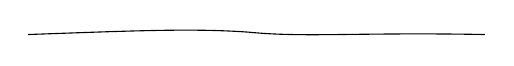
\begin{tikzpicture}
\draw (0,0) .. controls (1.4,.05) and (2.1,.08) .. (2.8,.03)
.. controls (3.5,-.04) and (4.2,.03) .. (5.8,0);
\end{tikzpicture}}

\textcircled{c}\quad On a
\[
(13)\qquad
N_\rho^*=\left\{u\in\mathcal M\mid u(\rho)=\rho^{\varepsilon_3(u)}\right\}
\quad\inserted{\bigl(=\varepsilon_3[\tau'](\rho)\bigr)}
\]

et
\[
(14)\qquad
\left\{\begin{aligned}
N_\rho^*\cap\widehat{\mathcal G}
  &=\mathbb D_\rho=\{1,\tau'\}.L_\rho\\
N_\rho^*\cap\mathcal G
  &=L_\rho\qquad(\simeq\mathbb Z/6\mathbb Z)\\
N_\rho^*\cap\Pi&=\mu\\
N_\rho^*\cap\Pi_0&=\{1\}
\end{aligned}\right.\qquad .
\]
\scanpage{624}

Soit
\[
(15)\qquad
N_{\rho0}^{*!}\overset{\mathrm{dfn}}=N_\rho^*\cap\mathcal M_0^!,
\qquad N_\rho^{*!}=N_\rho^*\cap\mathcal M^!.
\]

on trouve
\[
(16)\qquad
N_{\rho0}^{*!}\subset Z_\rho
=\operatorname{Cent}_{\unsure{\mathcal M(0)|\mathcal M}}(\rho)
=\operatorname{Cent}_{\mathcal M}(L_\rho)
\]

et on note aussi
\[
(17)\qquad N_{\rho,0}^{*!}=Z_{\rho0}^{!}=\mathcal M'(-\bar j).
\]

On voit que l'hom $\mathcal M\to\gamma_{\rho,\sigma}
=\widetilde{\Gamma}_{\mathbb Q}$ induit un \uline{iso}

\( (\unsure{18}) \)\quad
\diagram{\begin{tikzcd}[column sep=large,row sep=small]
\mathcal M'(-\bar j)=Z_{\rho,0}^{!} \arrow[r,"\sim"] &
\gamma'_{\rho,\sigma}=\widetilde{\Gamma}_{\mathbb Q}
\arrow[d,phantom,"{\rotatebox{90}{$=$}\ \mathrm{dfn}}"]\\
&\{\gamma\in\gamma_{\rho,\sigma}\mid\varepsilon_3(\gamma)=1\}
\end{tikzcd}}

d'où on déduit des scindages en produits semi-directs
(voire produits directs)
\[
(19)\qquad
\left\{\begin{aligned}
\mathcal M'&\simeq\mathcal M'(-\bar j).\mathcal G^{+\wedge}\\
\mathcal M^{\prime!}&\simeq\mathcal M'(-\bar j).\Pi\\
\mathcal M_0^{\prime!}&\simeq\mathcal M'(-\bar j).\Pi_0\\
Z_\rho^!\unsure{=|\simeq}\unsure{N_\rho^{*!}}
  &\simeq\mathcal M'(-j)\times\mu\\
\deleted{\unsure{N_\rho^*}}Z_\rho
  &\simeq\mathcal M'(-j)\times L_\rho
\end{aligned}\right.\qquad .
\]

\deleted{La correspondance entre}
\diagram{\begin{tikzcd}
\deleted{\unsure{\mathcal M^{!\prime}[0]|\mathcal M^{\prime!}[0]}}
\arrow[r,"{\deleted{\sim}}"] & \deleted{\gamma'_{\rho,\sigma}}
\end{tikzcd}}
\deleted{et}
\diagram{\begin{tikzcd}[column sep=small]
\deleted{\mathcal M(-j)} \arrow[r,phantom,"{\deleted{\subset}}"]
\arrow[rr,bend right=25,"{\deleted{\sim}}"'] &
\deleted{N_\rho^*} & \deleted{\gamma_{\rho,\sigma}}
\end{tikzcd}}
\deleted{est définie par l'application}

\deleted{\( (18) \)}\quad
\diagram{\begin{tikzcd}
\deleted{\unsure{\mathcal M^{!\prime}[0]|\mathcal M^{\prime!}[0]}}
\arrow[r] & {}
\end{tikzcd}}
% ===== LM_C3-625-643: second pass, checked against the scans =====
\scanpage{625}
\mspage{616}

% L1
Soit maintenant
\[
\tag{\unsure{20}}
\mu_{\tau'}=\{1,\tau'\}\subset\mathcal{G}^{\wedge}
\]
% L3
alors \inserted{\unsure{$\mu_{\tau'}$ normalise $L_\rho$}},
\deleted{\unsure{ce}} car
\(\tau'(\rho)=\rho^{-1}\) d'où \(\tau'(L_\rho)=L_\rho\)
donc il normalise \(Z_\rho\unsure{\equiv|=}\operatorname{Cent}_{\mathcal{M}}(L_\rho)\), donc
aussi \(Z_\rho^!=Z_\rho\cap\mathcal{M}^!\)
(puisque \(\mathcal{M}^!\) est invariant \unsure{dans} \(\mathcal{M}\))
\(=Z_{\rho,0}^!\times\mu=\mathcal{M}'(-\bar{\jmath})\times\mu\).
% L9
\deleted{Soit} D'ailleurs
\(\mu_{\tau'}\cap Z_\rho^!\subset
\deleted{\unsure{\{1\}}}\mu_{\tau'}\cap\mathcal{M}^!=\{1\}\).
Soit
\[
\tag{21}
\mathcal{N}_\rho^?=\mu_{\tau'}\cdot Z_\rho^!
=\mu_{\tau'}\cdot
\underbrace{(Z_{\rho,0}^!\times\mu)}_{
\substack{\mathcal{M}(-\bar{\jmath})\times\mu\\
\simeq\Gamma_{\mathbb{Q}}^{\prime\sim}\times\mu}}
\quad\deleted{\unsure{\simeq\mathcal{M}_{\mathbb{Q}}\times\mu|\simeq\mathcal{M}_{0}\times\mu}}.
\]
\hfill (produit $\frac12$ direct)

% L13
On fera attention que contrairement à ce
que pourrait suggérer cette écriture,
\(\mu_{\tau'}\) ne normalise \uline{pas} \(Z_{\rho,0}^!\) --- sinon on
aurait une \unsure{décomposition|disposition} en produit
\[
\mathcal{N}_\rho^?=\mathcal{N}_{\rho,0}^?\times\mu,
\quad\text{où }\mathcal{N}_{\rho,0}^?
=\deleted{\unsure{Z_{\rho,0}^!\times\mu}}
\mu_{\tau'}\cdot\unsure{Z_{\rho,0}^?|Z_{\rho,0}^!},
\]
% L19
or il n'en est rien. On a une suite exacte
\[
\tag{22}
\diagram{\begin{tikzcd}[ampersand replacement=\&,column sep=large,row sep=small]
1\arrow[r] \& \mu\arrow[r] \& \mathcal{N}_\rho^?\arrow[r]
\& \gamma_{\rho,\sigma}\arrow[r,no head]\arrow[d,equal] \& 1\\
\& \& \& \Gamma_{\mathbb{Q}}^{\sim} \&
\end{tikzcd}}
\]
% L22
de sorte que \(\mathcal{N}_\rho^?\) est une quasi-section
de multiplicité $2$ de l'extension
\(\mathcal{N}_\rho^{*}\longrightarrow\gamma_{\rho,\sigma}\), --- de
\(\mathcal{M}\longrightarrow\gamma_{\rho,\sigma}=\Gamma_{\mathbb{Q}}^{\sim}\).
Ainsi on trouve

\margin{624}
\scanpage{626}

% L1
\[
\tag{23}
\left\{\begin{aligned}
\mathcal{M}&=\mathcal{N}_\rho^?\wedge_{\mu_2}\mathcal{G}^{+\wedge}\\
\unsure{\mathcal{N}_\rho^*}&=\mathcal{N}_\rho^?\wedge_{\mu_2}
\deleted{\unsure{\mathbb{Z}}}L_\rho
\simeq\mathcal{N}_\rho^?\times
\underbrace{L_{-\rho}}_{\simeq\mathbb{Z}/3\mathbb{Z}}
\end{aligned}\right.
\]
% L3
La \deleted{suite}\inserted{extension} (22) de
\(\gamma_{\rho,\sigma}\) par \(\mu\) est
l'extension notée \(\widetilde{\gamma}_{\rho\sigma}\) dans la section précédente,
elle est sûrement \uline{\unsure{non} \deleted{triviale}\inserted{\unsure{scindée}}}.
Elle donne naissance à un \unsure{hom} canonique
\[
\tag{24}
\diagram{\begin{tikzcd}[ampersand replacement=\&,column sep=large]
\gamma_{\rho,\sigma}\arrow[r,"\sim"]
\&\mathcal{N}_\rho^?/\mu\arrow[r]
\&\mathcal{N}_\rho^*/\mu.
\end{tikzcd}}
\]

% L9
\uline{Remarque} Pour bien faire, il faudrait
expliciter l'opération de \(\tau'\) sur
\(Z_\rho^!\simeq Z_{\rho,0}^!\times\mu
\xrightarrow{\sim}\Gamma_{\mathbb{Q}}^{\prime\sim}\times\mu\), en termes de
l'opération de l'image \(\tau_{\Gamma\deleted{\unsure{\mathbb Q}}}\) de \(\tau'\) sur
\(\Gamma_{\mathbb Q}^{\prime\sim}\) par \unsure{autom.} int.
(NB \(\tau_\Gamma\) n'est autre que l'élément de
\(\Gamma_{\mathbb Q}\subset\Gamma_{\mathbb Q}^{\sim}\), ``conjugaison complexe'')
et d'un \unsure{hom} de \(\Gamma_{\mathbb Q}^{\prime\sim}\) dans \(\mu\)
\inserted{i.e d'un ``caractère quadratique'' de \(\Gamma_{\mathbb Q}^{\prime\sim}\)}
--- il y a fort à parier que
celui-ci est justement \(\varepsilon_2\) --- de sorte
que \(\Gamma_{\mathbb Q}^{0\sim}\simeq
\Gamma_{\mathbb Q}^{\prime\sim}\cap\Gamma_{\mathbb Q}^{\prime\prime\sim}\)
apparaît comme invariant par \(\tau'\) \ldots
En somme, il y aurait lieu de reprendre l'étude
de l'extension faite dans la section précédente,
en \unsure{y partant} du point de vue des \(\alpha,\beta\) \unsure{associés},

\margin{625}
\scanpage{627}
\mspage{617}

% L1
dans l'optique actuelle, sans doute plus
simple. Il y aurait lieu en $\overline{\mathrm m}$ temps
de \deleted{définir}\inserted{expliciter} une autre section partielle,
qui \deleted{mériterait} serait au dessus de
\(\deleted{\unsure{\Gamma}}\Gamma_{\mathbb Q}^{\prime\prime\prime\sim}\),
\[
\Gamma_{\mathbb Q}^{\prime\prime\prime\sim}
=\{x\in\Gamma_{\mathbb Q}^{\sim}\mid
\varepsilon_2(x)\varepsilon_3(x)=1\},
\]
% L6
et qui mériterait peut-être la notation
\(\mathcal{M}(\sqrt3)\) \unsure{ou du moins}
\(\mathcal{M}(q)\), pour
un générateur \(\unsure{q|\rho}\) convenable de \(\mathbb{Q}(\sqrt3)\) ???
\margin{?\quad\uline{\unsure{Méditer ces}}
\uline{\unsure{coïncidences.} \unsure{Attentif.|attentiv.}}}

% L9
Je me rends compte que je suis en train
de \unsure{déconner} --- ayant un peu perdu contact
avec le contenu géométrique de mes
calculs. Il faut garder à l'esprit que
\[
\tag{25}
\diagram{\begin{tikzcd}[ampersand replacement=\&]
\mathcal{M}_0^!\arrow[r,"\sim"] \& \mathcal{M}_{0,3}^{!\sim}
\end{tikzcd}}
\]
% L14
correspond \unsure{au} $\sim$ près, au \(\pi_1\) de \(U_{0,3\mathbb Q}\),
les sections de \(\mathcal{M}_0^!\longrightarrow
\Gamma_{\mathbb Q}^{\sim}\simeq\gamma_{\rho,\sigma}\) correspondent
donc (au $\sim$ près) à celles de
\(\pi_1(U_{0,3\mathbb Q})\) sur \(\Gamma_{\mathbb Q}\),
donc (``\unsure{invariablement|inévitablement|inavouablement}'') aux points
\inserted{\unsure{rat./$\mathbb Q$}} de \(U_{0,3\mathbb Q}\)
--- quand ce sont des sections partielles, aux
points de \(U_{0,3\mathbb Q}\) à valeurs dans des extensions
finies de \(\mathbb Q\). Ainsi, \deleted{les} la section
\deleted{\unsure{privilégiée}}\inserted{envisagée}
dans b) correspond bien au \(\mathrm{pt}\ \frac12\) de \(U_{0,3\mathbb Q}\),
la \deleted{\unsure{quasi-}}section
\inserted{partielle \(\mathcal M(-\bar\jmath)\)} envisagée ici dans c) correspond au
point \(-\bar\jmath\) de \(U_{0,3\mathbb Q}\), qui est dans
\(U_{0,3\deleted{\unsure{\mathbb Q}}}(\mathbb Q[\sqrt[3]{1}])\),
donc la notation \inserted{\(\mathcal M(-\bar\jmath)\)} est raisonnable.
Quant à \(\mathcal N_\rho^{\sim}\),
elle n'est \uline{pas} \(\subset\mathcal M_0^!\) --- $\overline{\mathrm m}$ en divisant par \(\mu\);
on trouve après division par \(\mu\) une section

\margin{626}
\scanpage{628}

% L1
de \(\mathcal M_{0,3}^{\sim}\) sur \(\Gamma_{\mathbb Q}^{\sim}\), mais ce n'est pas une
section de \(\mathcal M_{0,3}^{!\sim}\). Or au $\sim$ près, \(\mathcal M_{0,3}^{\sim}\)
est le \(\pi_1\) de \(M_{1,1\mathbb Q}'\), schéma modulaire sur \(\mathbb Q\)
des courbes elliptiques \uline{mod symétrie}.
Donc la donnée de cette section correspond à
la donnée d'une telle ``courbe elliptique
mod symétrie'' sur \(\mathbb Q\). Passant au \deleted{sous}
sous-groupe \(\Gamma_{\mathbb Q}^{\prime\sim}\) --- ce qui correspond à l'extension
du corps de base de \(\mathbb Q\) à \(\mathbb Q(j)=\mathbb Q(\sqrt[3]{1})\)
on retrouve l'image dans \(\mathcal M_{0,3}^{!\sim}\) de la \deleted{quasi-}
section \inserted{partielle} précédente --- \deleted{il} à \(\mathcal M(-\bar\jmath)\)
--- cela montre donc qu'il s'agit toujours de la ``$\overline{\mathrm m}$'' courbe
elliptique. J'ai donc l'impression \deleted{que} cependant
que sur \(\Gamma_{\mathbb Q}^{\sim}\) tout entier, cette section de
\(\mathcal M_{0,3}^{\sim}\) ne peut se remonter en une section
de \(\unsure{\mathcal M_\mu|\mathcal M}\) sur \(\Gamma_{\mathbb Q}^{\sim}\)
--- i.e justement que l'ext. \(\mathcal N_\rho^{\unsure{?|*}}\)
de \(\Gamma_{\mathbb Q}^{\sim}\) par \(\mu\) est non triviale.
Cela \uline{signifierait}-il qu'il n'existe pas de courbe elliptique
déf/\(\mathbb Q\) d'invariant $0$ ? (Chose que semble absurde
--- on doit pouvoir sur \uline{un corps} donner n'importe
quel invariant\ldots). \margin{?}
De façon précise, on a le
diagramme de schémas modulaires sur \(\mathbb Q\)
\[
\tag{26}
\diagram{\begin{tikzcd}[ampersand replacement=\&,column sep=large,row sep=large]
\begin{gathered}\text{sch. mod.}\\\text{des courbes}\\\text{ell.}\end{gathered}
\&M_{1,1}\arrow[d,"\substack{\text{gerbe}\\\text{de gr. }\mu}"]\arrow[dr]
\& \&\\
\begin{gathered}\text{sch. mod. des}\\\text{courbes ellipt.}\\\text{mod symétrie}\end{gathered}
\&M_{1,1}'\arrow[r]
\&\underset{\unsure{0|\circ}}{\mathbb E^1}
\&\begin{gathered}\text{schéma modulaire}\\\text{grossier}\end{gathered}
\end{tikzcd}},
\]
% L26
le fait qu'un point de \(M_{1,1}'(\mathbb Q)\) ne se re-

\margin{627}
\scanpage{629}
\mspage{618}

% L1
monte pas en un point de \(M_{1,1}\), ne \uline{signifie}
pas que son image dans \(\mathbb E^1\) ne se remonte pas
à \(M_{1,1}\). De façon précise, le \deleted{\illegible{1}}\inserted{diagramme}
s'identifie à :
\[
\tag{27}
\diagram{\begin{tikzcd}[ampersand replacement=\&,column sep=large,row sep=large]
M_{1,1}\simeq(U_{0,3},\widetilde{\mathcal G}_3)
  \arrow[d]\arrow[dr]\&\\
M_{1,1}'\simeq(U_{0,3},\mathcal G_3)\arrow[r]
  \&U_{0,3}/\mathcal G_3\simeq U_{0,3}/\widetilde{\mathcal G}_3
     \simeq\mathbb E^1
\end{tikzcd}},
\]
% L7
où \(\widetilde{\mathcal G}_3\) est l'extension de
\(\mathcal G_3\)\inserted{\(=\mathrm{SL}(2,\mathbb Z/2\mathbb Z)\)}
par \(\mu\), définie par
\[
\tag{28}
\begin{aligned}
\widetilde{\mathcal G}_3
 &=\mathcal G^+/\pi_0
 \simeq\mathrm{SL}(2,\mathbb Z)/
 \begin{gathered}
 \text{sous-groupe invariant}\\
 \text{engendré par}\\[-2pt]
 -\ell_0
 \end{gathered}
 \\
 &\simeq\mathrm{SL}(2,\mathbb Z/4\mathbb Z)/
 \begin{gathered}
 \text{sous-groupe}\\
 \text{invariant}\\
 \text{(d'ordre 4) engendré}\\
 \text{par }-\ell_0,\ \text{i.e \unsure{s\textsuperscript{s}groupe|s\textsuperscript{t}groupe}}\\
 \text{engendré par}\\
 -\ell_0,-\ell_1.
 \end{gathered}
\end{aligned}
\]
% L13
en faisant opérer \(\widetilde{\mathcal G}_3\) sur \(U_{0,3}\) par l'intermédiaire
de \(\mathcal G_3\). Un pt de \(M_{1,1}'\)\inserted{\unsure{rat/\(\mathbb Q\)}}
s'identifie \(\mathcal G_3\)-torseur \inserted{\(T\)} sur \(\mathbb Q\), muni
d'une application
\[
\tag{29}
\diagram{\begin{tikzcd}[ampersand replacement=\&]T\arrow[r]\&U_{0,3}\end{tikzcd}}
\]
\margin{\(T\) est le torseur
\inserted{\unsure{sous \(\mathrm{SL}(2,\mathbb Z/2\mathbb Z)\)}}
des \unsure{rigidifications|privilégiations} des points d'ordre $2$ et
\(\widetilde T\) celui des ``\unsure{pri-rigidifications|privilégiations|rigidifications}
des points d'ordre \(\unsure{\leq4|4}\)
\unsure{précisées}'' (le premier est défini
pour une courbe \unsure{ellipt.} mod symétrie, et
le $2^{\text{ième}}$ seulement pour une vraie courbe
elliptique)}
% L18
comp. avec les actions de \(\mathcal G_3\), un
point de \deleted{\(U_{0,3}\)} \(M_{1,1}\) s'identifie à un \(\widetilde{\mathcal G}_3\)-torseur
\(\widetilde T\) sur \(\mathbb Q\), muni d'une application
\[
\tag{30}
\diagram{\begin{tikzcd}[ampersand replacement=\&]\widetilde T\arrow[r,no head]\&U_{0,3}\end{tikzcd}}
\]
comp. avec l'opération de \(\widetilde{\mathcal G}_3\). \uline{Désignant}
par \deleted{\unsure{\(T\)}}
\[
T=\widetilde T/\mu
\]
le \(\mathcal G_3\)-torseur correspondant, la donnée de
(30) équivaut à la donnée de (29). Donc les

\margin{628}
\scanpage{630}

% L1
relèvements à \(M_{1,1}\) d'un point de \(M_{1,1}'\) rat/\(\mathbb Q\)
s'identifient aux \inserted{\(\widetilde{\mathcal G}_3\)-}torseurs \(\widetilde T\)
qui relèvent le \(\mathcal G_3\)-torseur \(T\), i.e. (à isom près) ils correspondent
aux hom \(\Gamma_{\mathbb Q}\longrightarrow\widetilde{\mathcal G}_3\)
qui relèvent l'hom
\(\Gamma_{\mathbb Q}\longrightarrow\mathcal G_3\) qui définit \(T\) :
\margin{on suppose \unsure{maintenant} choisi
un pt \deleted{\unsure{géom.}} de \(T(\overline{\mathbb Q}_0)\)}
\[
\diagram{\begin{tikzcd}[ampersand replacement=\&,column sep=large,row sep=small]
\&\widetilde{\mathcal G}_3\arrow[d]\\
\Gamma_{\mathbb Q}\arrow[r]\arrow[ur,dashed]\&\mathcal G_3
\end{tikzcd}}
\quad -
\]
% L8
l'obstruction est, comme il se doit, une
extension de \(\Gamma_{\mathbb Q}\) par \(\mu_2\), i.e. un \unsure{élém}
de \(H^2(\mathbb Q,\mu_2)\simeq {}_2\mathrm{Br}(\mathbb Q)\).
Dans le cas qui nous occupe, l'image de \(T\) dans \(U_{0,3}\)
est formé de \(\{-\bar\jmath,\unsure{-j|-\bar\jmath}\}\)
qui est connexe sur \(\mathbb Q\),
\uline{donc \(\Gamma_{\mathbb Q}\longrightarrow\mathcal G_3\) est surjectif}.
\margin{\unsure{corrigé|erroné}, cf rectification plus bas}
De façon générale, \deleted{\unsure{on doit}} dans la traduction
galoisienne en termes de scindages
de \(\mathcal M_{0,3}\) sur \(\Gamma_{\mathbb Q}\), l'hom
\(\Gamma_{\mathbb Q}\longrightarrow\mathcal G_3\)
est le composé
\[
\diagram{\begin{tikzcd}[ampersand replacement=\&]
\Gamma_{\mathbb Q}\arrow[r,"\unsure{k|\kappa}"]
\&\mathcal M_{0,3}\arrow[r]\&\mathcal G_3
\end{tikzcd}},
\]
% L22
qui est trivial ssi \deleted{\unsure{\(\Gamma_{\mathbb Q}\)}}
\inserted{\(\unsure{k|\kappa}\)} est une section de
\deleted{de}
\[
\mathcal M_{0,3}^!=\operatorname{Ker}
 (\mathcal M_{0,3}\longrightarrow\mathcal G_3)
\]
sur \(\Gamma_{\mathbb Q}\). Ici on a une section de
\(\mathcal M_{0,3}^!\) \deleted{sur}\inserted{au dessus}
du sous-groupe \(\Gamma_{\mathbb Q}'\) d'indice $2$,
\deleted{donc l'image de \(\Gamma_{\mathbb Q}'\)}
\(\unsure{k|\kappa}\mid\Gamma_{\mathbb Q}'=1\), donc
\(\unsure{k|\kappa}(\Gamma_{\mathbb Q})\subset\mathcal G_3\)
est d'ordre $2$, on voit que

\margin{629}
\scanpage{631}
\mspage{619}

c'est le sous-groupe \inserted{$\{1,\dot{\sigma}_{\infty}\}$} de $\mathcal{G}_3$.
(car l'image de $\tau'\inserted{{}=\sigma\tau}\in\mathcal{M}_{0,3}$ dans $\mathcal{G}_3$
\deleted{\unsure{est}} (comme celle de $\tau$ est $1$) est égale à celle de
$\sigma=\sigma_{\infty}$, i.e. $\dot{\sigma}_{\infty}$. Cela signifie
que \deleted{\unsure{T}} l'on a
\[
T\simeq T_0\mathbin{\wedge}_{\{1,\dot{\sigma}_{\infty}\}}\mathcal{G}_3
\]
i.e. $T$ est déduit d'un $\mu$-torseur (i.e. d'une
ext. quadratique de $\mathbb{Q}$\unsure{)} --- savoir justement
$\mathbb{Q}(\sqrt[3]{1})=\mathbb{Q}(j))$ par extension des groupes
d'opérateurs \inserted{$\mu\longrightarrow\mathcal{G}_3\quad(-1\longmapsto\dot{\sigma}_{\infty})$}.
Donc, prenant l'image inverse de $\mu=\{1,\dot{\sigma}_{\infty}\}$ dans
$\widetilde{\mathcal{G}}_3$, on trouve une extension de $\mu$ par $\mu$
--- ça ne peut guère être que $\mathbb{Z}/4\mathbb{Z}$ ! --- que j'ai envie de noter $\mathcal{E}''$

\[
\diagram{\begin{tikzcd}[ampersand replacement=\&,column sep=1.3em,row sep=0.15em]
\&\& \mathbb{Z}/4\mathbb{Z}\arrow[d,equal] \&\&\\
1\arrow[r]\&\mu\arrow[r]\&\mathcal{E}''\arrow[r]\&\mu\arrow[r,no head]\&1
\end{tikzcd}}
\]

\margin{oui, c'est évident puisque $\sigma=\sigma_{\infty}$ dans
$\widetilde{\mathcal{G}}_3=\mathrm{SL}(2,\mathbb{Z})/\unsure{\Pi_0|\Pi}$
est bien d'ordre $4$, donc $\mathcal{E}''\simeq\mathbb{Z}/4\mathbb{Z}$
\unsure{canoniquement}\ldots}
et le \unsure{pb} d'obstruction est de trouver un remontage

\[
\diagram{\begin{tikzcd}[ampersand replacement=\&,column sep=3em,row sep=2em]
\mathcal{E}''\arrow[r,no head]\&\mu\\
\Gamma_{\mathbb Q}\arrow[u,dashed]\arrow[ur]\&
\end{tikzcd}}
\]
,
(qui \deleted{\unsure{l'on}} n'existe sûrement pas) --- donc
l'obstruction s'identifie comme l'extension de $\Gamma_{\mathbb Q}$ par $\mu$,
image inverse de l'extension $\mathcal{E}''$.
\margin{C'est évident en \unsure{effet|fait}, \unsure{qu'on|puisque} :
$(\Gamma_{\mathbb Q})_{\mathrm{ab}}\simeq\widehat{\mathbb Z}^{*}
\supset\mathbb Z_3^{*}$, or
$(\mathbb Z_3^{*})_4\simeq\mathbb Z/2\mathbb Z$
(\unsure{donc déjà sur} $\mathbb Z_3^{*}$ \unsure{ça ne se remonte pas}\ldots}
(Il faudrait regarder pourquoi, en termes

\margin{630}
\scanpage{632}

classiques, cette obstruction est \unsure{scindée}, quand on
passe au sous-groupe $\Gamma_{\mathbb Q}^{\prime\prime\prime}$ correspondant au
corps $\mathbb Q(\sqrt{3}))$

Ainsi, le point $\mathbb Q$-rationnel envisagé de
$M_{1,1}'$ ne se remonte pas en un pt $\mathbb Q$-rationnel de
$M_{1,1}$ --- Par contre, son image $\inserted{0}$ dans
$\mathbb E^1\simeq U_{0,3}/\mathcal G_3$ doit bien se
remonter --- i.e. il doit bien exister un
$\widetilde{\mathcal G}_3$-torseur $\widetilde P$, et un
$\widetilde{\mathcal G}_3$-hom
\deleted{$\unsure{P}$}

\[
\diagram{\begin{tikzcd}[ampersand replacement=\&,column sep=1.6em,row sep=0.1em]
\widetilde P\arrow[r]\&U_{0,3}\&\text{i.e.}\&P\arrow[r]\arrow[d,equal]\&U_{0,3}\\
\&\&\&\widetilde P/\mu\&
\end{tikzcd}}
\]
.

Considérons en effet le \inserted{sous-}schéma
\deleted{de $U_{0,3}$, image inverse}
\[
\deleted{\unsure{Q=P}}\qquad
Q=U_{0,3}\mathbin{\times}_{\mathbb E^1}\{0\}
\]
l'image inverse de $0$, soit
\[
P_0=Q_{\mathrm{red}}\ \deleted{\unsure{\simeq}}
\]
c'est un sous-schéma qui, sur un corps
$K\supset\mathbb Q(j)$, \deleted{se scinde en} est somme de
deux pts, et qui sur $\mathbb Q$ est connexe
--- c'est un schéma \inserted{can.\textsuperscript{l}} isomorphe à
$\operatorname{Spec}\mathbb Q(-\bar j)$. Il est stable par $\mathcal G_3$,
qui y opère via

\[
\diagram{\begin{tikzcd}[ampersand replacement=\&]
\mathcal G_3\arrow[r,"\mathrm{sg}"]\&\mu
\end{tikzcd}}
\]

et l'opération galoisienne de $\mu$ sur le $\mu_{\mathbb Q}$-torseur $P_0$.

\margin{631}
\scanpage{633}
\mspage{620}

Ainsi on a le diagramme

\[
\diagram{\begin{tikzcd}[ampersand replacement=\&,column sep=1.8em,row sep=2em]
\&\widetilde{\mathcal G}_3\arrow[r,"\mathrm{can}"]\&\mathcal G_3\arrow[r,"\mathrm{sg}"]\&\mu\\
(31)\&\&\Gamma_{\mathbb Q}\arrow[ur]\&
\end{tikzcd}}
\]

\margin{\uline{NB} le noyau de
$\widetilde{\mathcal G}_3\longrightarrow\mu$ est une
extension \inserted{centrale} de $\mathbb Z/3\mathbb Z$
par $\mu=\mathbb Z/2\mathbb Z$, elle
est donc \unsure{trivial} et
isom. à $\mathbb Z/6\mathbb Z$
(noyau engendré par $\rho$).}

On voit donc que la catégorie des relèvements
du pt $\mathbb Q$-rationnel $0$ de $\mathbb E^1$ en un
pt $\mathbb Q$-rationnel de $M_{1,1}'$ resp. $M_{1,1}$, est
équivalente à celle des $\mathcal G_3$-torseurs \inserted{$P$} resp\unsure{.}
des $\widetilde{\mathcal G}_3$-torseurs \inserted{$\widetilde P$} sur $\mathbb Q$, qui relèvent le
$\mu$-torseur $P_0$. On avait choisi un
$P=T$ de façon \unsure{particulièrement} \unsure{trivial|triviale},
en utilisant le scindage

\[
\diagram{\begin{tikzcd}[ampersand replacement=\&,column sep=1.5em]
\mu\arrow[r,"\sim"]\&\{1,\dot\sigma_{\infty}\}\arrow[r,hook]\&\mathcal G_3
\end{tikzcd}}
\]

de $\mathcal G_3\longrightarrow\mu$ --- mais le torseur $T$ ne se
remonte pas en un $\widetilde T$. Les classes d'isomorphie de pts de $M_{1,1}'$ resp. de $M_{1,1}$ au-dessus
du pt $0$ de $\mathbb E^1$, \unsure{correspondent} de $\overline{\mathrm m}$ aux
classes de conjugaison \inserted{(mod noyaux \inserted{$\mathcal G_3^+,\widetilde{\mathcal G}_3^+$} de $\mathcal G_3\longrightarrow\mu$ et $\widetilde{\mathcal G}_3\longrightarrow\mu$)} de relèvements de
$\Gamma_{\mathbb Q}\longrightarrow\mu$ en $\Gamma_{\mathbb Q}\longrightarrow\mathcal G_3$ resp. en $\Gamma_{\mathbb Q}\longrightarrow\widetilde{\mathcal G}_3$.

\deleted{\unsure{De là}} Considérons un relèvement en

\[
\diagram{\begin{tikzcd}[ampersand replacement=\&]
\Gamma_{\mathbb Q}\arrow[r]\&\mathcal G_3
\end{tikzcd}}
\]
,
son image est un sous-groupe de $\mathcal G_3$, qui est soit

\margin{632}
\scanpage{634}

$\{1,\dot\sigma_{\infty}\}$ ou un de ses conjugués,
$\{1,\dot\sigma_0\}$, $\{1,\unsure{\bar\sigma_1|\dot\sigma_1}\}$,
\uline{ou} c'est $\mathcal G_3$ tout entier. Dans le premier
cas, on a vu que ça ne se remonte pas
en $\widetilde{\mathcal G}_3$. Donc pour pouvoir remonter,
il faut prendre un \uline{épi} $\Gamma_{\mathbb Q}\longrightarrow\mathcal G_3$ ---
on sort donc du cadre abélien sur
$\mathbb Q$, pour entrer dans le domaine des
extensions abéliennes de $\mathbb Q(j)$.

Examiner en termes des groupes de
Galois s'il existe un tel relèvement \deleted{qui}
$\Gamma_{\mathbb Q}\longrightarrow\widetilde{\mathcal G}_3$, et \deleted{\unsure{quel}}
comment les obtenir,
apparaît comme un exercice plaisant
et \unsure{délectable} de théorie des corps de
classes, que je ne vais pas poursuivre
pour le moment, pour ne pas éterniser
cette digression. Revenant par la suite
sur ce point, il me faudrait en $\overline{\mathrm m}$
temps expliciter la relation entre les
\unsure{prises|points} de un remontage d'l'hom de $\Gamma_{\mathbb Q}$,
et scindages de l'extension $\mathcal M_{0,3}$ de $\Gamma_{\mathbb Q}$
par $\unsure{\mathcal G_{0,3}^{+\wedge}|\widetilde{\mathcal G}_{0,3}^{+\wedge}}$,
ou $\mathcal M$ de $\Gamma_{\mathbb Q}$ par
$\mathcal G^{+\wedge}\simeq\mathrm{SL}(2,\mathbb Z)^\wedge$.

\margin{633}
\scanpage{635}
\mspage{621}

Revenons aux sous-groupes \deleted{$\unsure{\mathcal N_{\rho}^{?}}$ de}

\[
\diagram{
\begin{tikzcd}[ampersand replacement=\&,column sep=3em,row sep=2em]
\mathcal N_{\rho}^{?}
  \arrow[r,phantom,"{\overset{3}{\unsure{\subset}}}"{description}]
\&\mathcal N_{\rho}^{*}\arrow[r,phantom,"{\subset}"{description}]
\&\mathcal M\\
Z_{\rho,0}^{!}=\mathcal M'(-\bar j)
  \arrow[u,phantom,"{4\,\cup}"{description}]
\&\&
\end{tikzcd}
}
\]

contenant \unsure{la|le} \deleted{section}\inserted{\unsure{sous-groupe|sous-groupes}}
partielle $\mathcal M(-\bar j)\simeq\widetilde\Gamma_{\mathbb Q}'$.

Soit
\[
\tag{32}
\begin{aligned}
\mathcal M^0(-\bar j)&\overset{2}{\subset}\mathcal M'(-\bar j)\\
\underset{\unsure{\mathrm{dfn}|\mathrm{def}}}{=}&\operatorname{Ker}
\bigl(\mathcal M'(-\bar j)\xrightarrow{\varepsilon_2}\mu\bigr)
=\deleted{\unsure{\mathcal N_{\rho}^{?}|\mathcal M}}\,Z_{\rho}
\cap\deleted{\unsure{\operatorname{Ker}\varepsilon_2}}\,
\mathcal M_0^{\prime\prime!}\\
&=\mathcal N_{\rho}^{*}\cap\mathcal M_0^{0!}
\end{aligned}
\]
qui est donc une section partielle \unsure{en|au} dessus de
\[
\tag{33}
\begin{aligned}
\widetilde\Gamma_{\mathbb Q}^0
&=\operatorname{Ker}\bigl(\widetilde\Gamma_{\mathbb Q}
\xrightarrow{(\varepsilon_2,\varepsilon_3)}\mu\times\mu\bigr)
\deleted{\unsure{\ne|=}\widetilde\Gamma_{\mathbb Q}}\\
&=\operatorname{Ker}\bigl(\widetilde\Gamma_{\mathbb Q}
\longrightarrow\widehat{\mathbb Z}^{*}\longrightarrow
(\mathbb Z/12\mathbb Z)^{*}\bigr)
\end{aligned}
\]

\deleted{Considérons} Modulo une vérification
que je vais faire plus bas, $\tau'$ normalise
\deleted{(34)}
$\mathcal M^0(-\bar j)$, considérons \unsure{les|le}
\[
\tag{34}
\mathcal M'''(-\bar j)\deleted{\unsure{\mathcal N_{\rho,0}^{?}}}
\overset{\unsure{\mathrm{dfn}|\mathrm{def}}}{=}
\underset{\text{(semi-direct)}}{\mu_{\tau'}\mathbin{.}\mathcal M^0(-\bar j)}
\qquad\text{où }\mu_{\tau'}=\{1,\tau'\}
\]
c'est un sous-groupe d'indice $4$ de $\mathcal N_{\rho}^{?}$,
et on a maintenant
\[
\tag{35}
\deleted{\unsure{\mathcal N_{\rho,0}^{?}}}\quad
\mathcal M'''(-\bar j)\xrightarrow{\sim}\widetilde\Gamma_{\mathbb Q}''',
\]
c'est une section partielle \unsure{en|au} dessus
de $\widetilde\Gamma_{\mathbb Q}'''$, d'où des isomorphismes

\margin{634}
\scanpage{636}

\deleted{
\[
\tag{36}
\left\{
\begin{aligned}
\mathcal M'''&\simeq\mathcal M'''(-\bar j)\mathbin{.}\mathcal G^{+\wedge}\\
\deleted{\unsure{\mathcal M'''}}\,\mathcal N_{\rho}^{*}
&\simeq\mathcal M'''(-\bar j)\mathbin{.}L_{\rho}.
\end{aligned}
\right.
\]

On a le diagramme récapitulatif
d'inclusions de sous-groupes de $\mathcal N_{\rho}^{*}$

\[
\diagram{
\begin{tikzcd}[ampersand replacement=\&,column sep=2.5em,row sep=1.5em]
\&\&\&Z_{\rho}\arrow[dr,hook,"2"]\&\\
\&\&\begin{gathered}\mathcal M'(-\bar j)\\=Z_{\rho,0}^{!}\end{gathered}
  \arrow[ur,hook,"6"]\arrow[dr,hook,"4"]
\&\&\mathcal N_{\rho}^{*}\\
(37)\&\mathcal M^0(-\bar j)\arrow[ur,hook,"2"]\arrow[dr,hook,"2"']
\&\&\mathcal N_{\rho}^{?}\arrow[ur,hook,"3"']\&\\
\&\&\mathcal M'''(-\bar j)\arrow[ur,hook,"4"]\&\&
\end{tikzcd}
}
\]


Notons que l'inclusion
\[
\tag{38}
\underset{\substack{\simeq\\\unsure{\mathbb D_6|\mathbb D_{\sigma}}}}{\mathbb D_{\rho}}
\overset{\mathrm{dfn}}{=}
\underset{\simeq\mathbb Z/2\mathbb Z}{\uline{\mu_{\tau'}}}
\mathbin{.}
\underset{=\mathbb Z/6\mathbb Z}{\uline{L_{\rho}}}
\subset\mathcal N_{\rho}^{*}
\]
induit un isomorphisme d'
\[
\tag{39}
\mathbb D_{\rho}\xrightarrow{\sim}\mathcal N_{\rho}^{*}/
\]
}

\margin{635}
\scanpage{637}
\mspage{622}

\[
\tag{36}
\left\{
\begin{aligned}
\mathcal{M}'''&\simeq \mathcal{M}'''(-\bar j)\mathbin{.}\mathcal{G}^{+\wedge}\\
\mathcal{N}_{\rho}^{*}&\simeq \mathcal{M}'''(-\bar j)\mathbin{.}L_{\rho}.
\end{aligned}
\right.
\]

Diagramme récapitulatif des sous-groupes de $\mathcal{N}_{\rho}^{*}$
obtenus jusqu'à présent:


\[
\diagram{
\begin{tikzcd}[ampersand replacement=\&,column sep=1.05em,row sep=2.8em]
\&\& \mathcal{M}^{0}(-\bar j)
  \arrow[rr,hook,"2"]
  \arrow[dl,hook,"2"']
\&\& \begin{gathered}\mathcal{M}'(-\bar j)\\=Z_{\rho,0}^{!}\end{gathered}
  \arrow[rr,hook,"2"]
  \arrow[dl,hook,"2"']
  \arrow[dr,no head,draw=gray,
    "{\unsure{\mathcal{M}'(-\bar j)\times\mu}}"{description,pos=.5},
    "{\unsure{\searrow}}"{pos=.93}]
\&\& \mathcal{M}'(-\bar j)\times\mu
  \arrow[rr,hook,"3"]
  \arrow[dl,hook,"2"']
\&\& Z_{\rho}\arrow[dl,hook,"2"']\\
(37)\&\mathcal{M}'''(-\bar j)\arrow[rr,hook,"2"]
\&\& \mathcal{M}'''(-\bar j)\times\mu\arrow[rr,hook,"2"]
\&\& \mathcal{N}_{\rho}^{?}\arrow[rr,hook,"3"]
\&\& \mathcal{N}_{\rho}^{*}
\&\&\\
\&\&\&\&1
  \arrow[uu,hook]
  \arrow[uull,hook,start anchor=north west,end anchor=south west]
  \arrow[rr,hook,"2"]
  \arrow[dl,hook,"2"']
\&\&\mu\arrow[uu,hook]\arrow[rr,hook,"3"]\arrow[dl,hook,"2"']
\&\&L_{\rho}\arrow[uu,hook]\arrow[dl,hook,"2"']\\
\&\&\&\mu_{\tau'}\arrow[uu,hook]\arrow[uull,hook]\arrow[rr,hook,"2"]
\&\&\mathbb{D}_{\tau'}\arrow[uu,hook]\arrow[rr,hook,"3"]
\&\&\mathbb{D}_{\rho}\arrow[uu,hook]
\end{tikzcd}
}
\]
,

où nous sommes ici intéressés \unsure{surtout} à la
“face supérieure”, \unsure{contenant|concernant} des sous-groupes d'indice fini de
$\mathcal{N}_{\rho}^{*}$, intermédiaires entre celui-ci et
$\unsure{\mathcal{M}_{0}(-\bar j)|\mathcal{M}^{0}(-\bar j)}$
(d'indice $24$ dans $\mathcal{N}_{\rho}^{\unsure{*}}$).
Je vais examiner la question d'invariance de ces sous-groupes
les uns dans les Autres, et la structure des groupes quotients.

Je vais refaire un diagramme qui montre \unsure{vraiment|mieux} les
\deleted{\unsure{groupes|rapports}} relations entre les groupes en question.

\margin{636}
\scanpage{638}


\[
\diagram{
\begin{tikzcd}[ampersand replacement=\&,column sep=.6em,row sep=1.3em,cells={font=\scriptsize}]
\&\&Z_{\rho}\arrow[rrr,hook,"2"]
  \arrow[ddddll,dashed,leftrightarrow,bend right=35,
    "{\unsure{\leftrightarrow}}"'{description}]
\&\&\&\mathcal{N}_{\rho}^{*}\\
\&\&\&Z_{\rho,0}^{!}=\mathcal{M}'(-\bar j)
  \arrow[rrr,hook,"2"]
  \arrow[dl,hook,"2"']
\&\&\&\mathcal{M}'(-\bar j)\mathbin{.}\mu_{\tau'}\;{}^{*}
  \arrow[dl,hook,"2"']\\
\&\&Z_{\rho}^{!}=\mathcal{M}'(-\bar j)\times\mu
  \arrow[uu,hook,"3"']
  \arrow[rrr,hook,"2"]
  \arrow[ddll,hook,dashed,"3"']
\&\&\&\mathcal{N}_{\rho}^{?}
  \arrow[uu,hook,"3"']
  \arrow[ddll,hook,dashed,"3"']\\
\&\&\&\mathcal{M}^{0}(-\bar j)
  \arrow[uu,hook,"2"']
  \arrow[rrr,hook,"2"]
  \arrow[ddl,hook,"2"']
\&\&\&\mathcal{M}'''(-\bar j)
  \arrow[uu,hook,"2"']
  \arrow[ddl,hook,"2"']\\
Z_{\rho}\arrow[rrr,hook,dashed]
\&\&\&\unsure{\mathcal{N}_{\rho}|\mathcal{N}_{\rho}^{*}}
  \arrow[uuuurr,dashed,leftrightarrow,bend left=20,
    "{\unsure{\leftrightarrow}}"'{description}]\\
\&\&\mathcal{M}^{0}(-\bar j)\times\mu
  \arrow[uuu,hook,"2"']
  \arrow[rrr,hook,"2"]
  \arrow[dddll,hook,
    "{\deleted{\unsure{\hookrightarrow}}}"{description}]
\&\&\&\mathcal{M}'''(-\bar j)\times\mu
  \arrow[uuu,hook,"2"']
  \arrow[dddll,hook,
    "{\deleted{\unsure{\hookrightarrow}}}"{description}]\\
\&\&\&1\arrow[uuu,hook]
  \arrow[rrr,hook,"2"]
  \arrow[dl,hook,"2"']
\&\&\&\mu_{\tau'}\arrow[uuu,hook]\arrow[dl,hook,"2"']\\
(38)\&\&\mu\arrow[uu,hook]\arrow[rrr,hook,"2"]
  \arrow[ddll,hook,dashed,"3"']
\&\&\&\mathbb{D}_{\tau'}\arrow[uu,hook]
  \arrow[ddll,hook,dashed,"3"']\\
\deleted{\unsure{L_{\rho}}}
  \arrow[rrr,hook,
    "{\deleted{\unsure{\hookrightarrow}}}"{description}]
\&\&\&\deleted{\unsure{\mathbb{D}_{\rho}}}\\
L_{\rho}\arrow[uuuuu,hook,dashed]
  \arrow[rrr,hook,dashed,"2"]
\&\&\&\mathbb{D}_{\rho}\arrow[uuuuu,hook,dashed]
\end{tikzcd}
}
\]


\margin{$*$ -- Attention,
$\mathcal{M}'(-\bar j)\mathbin{.}\mu_{\tau'}$ n'est \uline{pas}
un sous-groupe, car $\mu_{\tau'}$ ne normalise pas
$\mathcal{M}'(-\bar j)$.}

\unsure{a)} Sous-groupes d'indice fini dans $Z_{\rho}$ -- dans le diagramme
il y en a quatre


\[
\diagram{
\begin{tikzcd}[ampersand replacement=\&,column sep=3em,row sep=3em]
\&Z_{\rho}^{!}=\mathcal{M}'(-\bar j)\times\mu
\&\mathcal{M}'(-\bar j)=Z_{\rho,0}^{!}=\mathcal{N}_{\rho,0}^{\unsure{*!}}
  \arrow[l,hook,"2"']\\
(39)\&\mathcal{M}^{0}(-\bar j)\times\mu
  \arrow[u,hook,"2"']
\&\mathcal{M}^{0}(-\bar j)=Z_{\rho,0}^{0!}
  \arrow[u,hook,"2"]
  \arrow[l,hook,"2"]
\end{tikzcd}
}
\]


sont ils invariants dans $Z_{\rho}$? C'est clair pour les sous-groupes
\deleted{$\unsure{\mathcal{M}'(-\bar j)}$}
\[
\tag{40}
\left\{
\begin{aligned}
\mathcal{M}'(-\bar j)\times\mu
  &=Z_{\rho}\cap\mathcal{M}^{!}=Z_{\rho}^{!},
  \quad\text{et pour}\\
\deleted{\unsure{\mathcal{M}^{0}(-\bar j)\times\mu=}}&\\[-.5ex]
\mathcal{M}^{0}(-\bar j)\times\mu
  &=Z_{\rho}\cap\mathcal{M}^{!}\cap
       \operatorname{Ker}(\varepsilon_{2}:\mathcal{M}\to\mu)
\end{aligned}
\right.
\]
-- cela montre que ces groupes sont

\margin{637}
\scanpage{639}
\mspage{623}

même invariants dans $\mathcal{N}_{\rho}^{*}$, puisque
\deleted{$\unsure{\mathcal{M}^{!}}$}.
$Z_{\rho},\mathcal{M}^{!},\operatorname{Ker}\varepsilon_{2}$
sont stabilisés par $\mathcal{N}_{\rho}^{*}$.
D'ailleurs, \deleted{comme}
$Z_{\rho,0}^{!}=\mathcal{M}'(-\bar j)$ est
\deleted{d'indice $2$}\inserted{invariant}
\deleted{\unsure{dans}}\inserted{dans}
$Z_{\rho}^{!}=\mathcal{M}'(-\bar j)\times\mu$,
\unsure{pour} montrer qu'il l'est dans $Z_{\rho}$, il suffit de prouver
qu'il est normalisé par $\rho$
(puisque $Z_{\rho}=L_{\rho}\mathbin{.}Z_{\rho}^{!}$ -- c'est
$\pm$ trivial), or examinons de façon générale pour
\deleted{$\unsure{x\in}$} $x\in\mathcal{M}$
si $x$ normalise \deleted{$\unsure{\mathcal{M}_{0}^{!}}$}
\[
\mathcal{M}_{0}^{!}\overset{\mathrm{dfn}}{=}
\mathcal{M}(0)\mathbin{.}\Pi_{0},
\]
Comme il normalise $\Pi_{0}$, il suffit de voir si
pour $u\in\mathcal{M}(0)$, on a
\[
xux^{-1}\in\mathcal{M}_{0}^{!}
\]
ce qui équivaut aussi à
\[
xux^{-1}\equiv u\qquad(\Pi_{0})
\]
i.e.
\[
[x,u]\in\Pi_{0}
\]
or on sait que pour $x\in\mathcal{G}$,
\inserted{$u\in\mathcal{M}^{!}$,} on a
\[
\tag{*}
\underbrace{[x,u]}_{\inserted{x\,u(x)^{-1}}}^{\unsure{c}}
\equiv
(\operatorname{sg}(x))^{\inserted{\unsure{\xi_{2}(u)|\varepsilon_{2}(u)}}}
\deleted{\unsure{\xi_{2}(u)|\varepsilon_{2}(u)}}
\quad\mathrm{mod}\ \Pi_{0}
\]
où

\[
\diagram{
\begin{tikzcd}[ampersand replacement=\&,column sep=2em]
\operatorname{sg}:\&
\mathcal{G}\arrow[r,"\mathrm{can}"]\&
\mathcal{G}_{3}\arrow[r,"\operatorname{sg}"]\&
\mu.
\end{tikzcd}
}
\]


Cela montre \deleted{\unsure{qu'on}} que

\uline{Lemme}
\[
\left\{
\begin{aligned}
&\text{Si }x\in\mathcal{G}^{+},\ u\in\mathcal{M}_{0}^{!},
  \quad\text{alors }
  \deleted{xux^{-1}\in\mathcal{M}_{0}^{!}}
  \ \text{conditions équivalentes}\\
&a)\quad xux^{-1}\in\mathcal{M}_{0}^{!}\\
&b)\quad xux^{-1}\equiv u\quad(\Pi_{0})
       \quad\text{i.e.}\quad [x,u]\in\Pi_{0}\\
&c)\quad .\operatorname{sg}(x)^{
       \inserted{\unsure{\xi_{2}(u)|\varepsilon_{2}(u)}}}
       \deleted{\unsure{\xi_{2}(u)|\varepsilon_{2}(u)}}=1
       \quad\text{i.e.}\quad
       \operatorname{sg}(x)=1\quad\text{\uline{ou}}\quad
       \varepsilon_{2}(u)=1
\end{aligned}
\right.
\]

\margin{638}
\scanpage{640}

\deleted{Pour $x=\rho$, cela montre que \unsure{le|la}
\deleted{\unsure{condition}}\inserted{\unsure{premier groupe}}
\unsure{est}}

\uline{Corollaire 1} Soit $x\in\mathcal{G}^{+\wedge}$.
Pour que $x$ normalise $\mathcal{M}_{0}^{!}$,
il faut s. qu'on ait $\operatorname{sg}(x)=+1$.

\uline{Corollaire 2}. Le sous-groupe
$\mathcal{M}_{0}^{\prime\prime!}
=\mathcal{M}''(0)\mathbin{.}\Pi_{0}$
est \deleted{invariant dans} normalisé par
$\mathcal{G}^{+\wedge}$.

Ceci montre en particulier que $\rho$ normalise
$\mathcal{M}_{0}^{!}$, donc aussi
$\inserted{\mathcal{M}'(-\bar j)=}
Z_{\rho,0}^{!}=Z_{\rho}\cap\mathcal{M}_{0}^{!}$,
qui est donc invariant dans $Z_{\rho}$.
Il en est donc de $\overline{\mathrm m}$ de son intersection
avec $\mathcal{M}^{0}(-\bar j)\times\mu$, soit
$\mathcal{M}^{0}(-\bar j)$.
(Ou encore; ce groupe est égal à
$Z_{\rho}\cap\mathcal{M}_{0}^{\prime\prime!}$,
et $\mathcal{M}_{0}^{\prime\prime!}$ est normalisé par $\rho\ldots$).
\uline{Ainsi les quatre groupes} $(39)$
\uline{sont distingués dans $Z_{\rho}$.} )

Pour voir s'ils sont distingués dans
$\unsure{\mathcal{N}_{\rho}^{*}}
=\mu_{\tau'}\mathbin{.}Z_{\rho}$,
il suffit de voir s'ils sont normalisés par $\tau'$.
C'est clair pour $Z_{\rho}^{!}=Z_{\rho}\cap\mathcal{M}^{!}$
-- d'où le fait que
$\mathcal{N}_{\rho}^{?}=\mu_{\tau'}\mathbin{.}Z_{\rho}^{!}$
est un sous-groupe de $\mathcal{N}_{\rho}^{*}$.
Pour
\deleted{$\mathcal{M}^{0}(-\bar j)=
Z_{\rho}\cap\mathcal{M}_{0}^{\prime\prime!}$, il}
\inserted{voir \deleted{\unsure{si les}} les quels des}
trois autres sous-groupes
\inserted{envisagés}
en dernier sont normalisés, il faudrait donc expliciter
l'action de $\tau'$ \deleted{dessus.}
sur $Z_{\rho}^{!}=\mathcal{M}'(-\bar j)\times\mu$.

\margin{639}
\scanpage{641}
\mspage{623}

Notons que $\tau\in\mathcal{M}(0)\subset\mathcal{M}_{0}^{!}$
normalise $\mathcal{M}_{0}^{!}$, donc
\deleted{\unsure{on|donc}}\inserted{il} opère
\deleted{$\unsure{Z}$} sur
$\mathcal{M}^{!}
=\underbrace{\mathcal{M}_{0}^{!}}_{\simeq\widetilde{\Gamma}_{\mathbb{Q}}\mathbin{.}\Pi_{0}}
\times\mu$
par l'opération produit de la conjugaison par $\tau$ dans
$\mathcal{M}_{0}^{!}$, et l'identité dans $\mu$.
On a d'autre part $\tau'=\tau\sigma$, on a vu que
\[
 (40)\qquad
 \sigma(x)\equiv\varepsilon_{2}(x)x\qquad(\Pi_{0})
 \qquad x\in\mathcal{M}
\]
donc
\[
 (41)\qquad
 \tau'(x)\equiv\varepsilon_{2}(x)\tau(x)\qquad(\Pi_{0})
 \qquad x\in\mathcal{M}
\]
donc il s'ensuit
\[
 (42)\quad
 \left\{
 \begin{aligned}
 &\text{si }x\in\mathcal{M}_{0}^{!},\quad
   \text{alors }\tau'(x)\equiv x\quad(\Pi_{0})
   \inserted{\Longleftrightarrow\tau'(x)\in\mathcal{M}_{0}^{!}}
   \Longleftrightarrow\varepsilon_{2}(x)=1\\
 &\text{en particulier, }\mathcal{M}_{0}^{\prime\prime!}
   \text{ est normalisé par }\tau
 \end{aligned}
 \right.
\]
Donc \deleted{si $x\in$} appliquant ceci aux éléments de
$Z_{\rho,0}^{!}=\mathcal{M}'(-\bar j)$ dans
$Z_{\rho}^{!}=\mathcal{M}'(-\bar j)\times\mu$,
on trouve
\[
 (43)\quad
 \left\{
 \begin{aligned}
 &\text{Soit }x\in Z_{\rho,0}^{!}=\mathcal{M}'(-\bar j),
   \text{ alors }\deleted{\unsure{\tau}}\\
 &\tau'(x)\in Z_{\rho,0}^{!}
   \Longleftrightarrow\varepsilon_{2}(x)=1
 \end{aligned}
 \right.
\]

\uline{Corollaire}\quad
$Z_{\rho,0}^{!}\inserted{=\mathcal{M}'(-\bar j)}$
n'est pas normalisé par $\tau'$, donc n'est pas invariant dans
$\unsure{\mathcal{N}_{\rho}^{*}}$,
mais \deleted{le}
$\mathcal{M}^{0}(-\bar j)=Z_{\rho}\cap\mathcal{M}_{0}^{\prime\prime!}$
est normalisé par $\tau'$, donc aussi son produit par $\mu$.

Donc le seul des quatre sous-groupes $(39)$ de $Z_{\rho}$
qui ne soit distingué dans $\mathcal{N}_{\rho}$ est
$\mathcal{M}'(-\bar j)=Z_{\rho,0}^{!}$.
Les autres donnent

\margin{640}
\scanpage{642}

naissance, par produit $\frac12$ direct avec $\mu_{\tau'}$,
à des \unsure{s-groupes|ss-groupes} de $\mathcal{N}_{\rho}$,
invariants dans $\mathcal{N}_{\rho}$.
Le plus petit de tous ces sous-groupes est
$\mathcal{M}^{0}(-\bar j)$, qui est d'indice $24$ dans
$\unsure{\mathcal{N}_{\rho}^{*}}$.
Le groupe quotient \deleted{\unsure{est un}}
\[
 \deleted{\unsure{\text{groupe}}}\qquad
 \mathcal{N}_{\rho}^{*}/\mathcal{M}^{0}(-\bar j)
\]
est donc un groupe d'ordre $24$, qui reçoit d'ailleurs le groupe
$\mathbb{D}_{\rho}
\inserted{=\mu_{\tau'}\mathbin{.}L_{\rho}}
\subset\mathcal{N}_{\rho}^{*}$,
normalisateur de $L_{\rho}$ dans
$\unsure{\operatorname{GL}}(2,\mathbb{Z})$,
groupe isomorphe à $D_{6}$, et d'ordre $12$.
Le noyau de

\[
\diagram{
 \begin{tikzcd}[ampersand replacement=\&]
 (44)\quad\mathbb{D}_{\rho}
 \arrow[r,hook] \&
 \mathcal{N}_{\rho}^{*}/
 \mathcal{M}^{0}(\bar j)
 \end{tikzcd}
}
\]

est évidemment contenu dans $L_{\rho}=\mathbb{D}_{\rho}\cap Z_{\rho}$
et il est réduit à $1$ car
puisqu'on a $\overline{\mathrm m}$
\[
 L_{\rho}\cap Z_{\rho,0}^{!}
 \subset L_{\rho}\cap\mathcal{M}_{0}^{!}
 =L_{\rho}\cap\Pi_{0}=\{1\}.
\]
Ainsi $\mathbb{D}_{\rho}\inserted{\text{(d'ordre }12\text{)}}$
apparaît comme un sous-groupe d'indice $2$ de
$\mathcal{N}_{\rho}^{*}/\mathcal{M}^{0}(-\bar j)$,
tout comme il est sous-groupe d'indice $2$ de
$\mathcal{G}/\Pi_{0}$. Il serait tentant

\margin{641}
\scanpage{643}
\mspage{624}

alors d'établir un isomorphisme
\[
 \mathcal{N}_{\rho}^{*}/\mathcal{M}^{0}(-\bar j)
 \overset{?}{\simeq}\mathcal{G}^{\wedge}/\Pi_{0}
\]
compatible avec ces plongements de $\mathbb{D}_{\rho}$.
Essayons-le \unsure{ainsi|aussi}:

\uline{Proposition}\quad Considérons l'hom. composé

\[
\diagram{
 \begin{tikzcd}[ampersand replacement=\&,column sep=large,row sep=large]
 (45)\quad\mathcal{M}\arrow[r,"\Theta_{\mathcal{M}}"]\&
 \operatorname{GL}(2,\widehat{\mathbb{Z}})
 \arrow[r]\&
 \operatorname{GL}(2,\mathbb{Z}/4\mathbb{Z})
 \arrow[r,"\substack{\text{épi. de}\\\text{degré }4}"]\&
 \begin{gathered}
 \mathcal{G}^{\unsure{*|\wedge}}/\Pi_{0}\\
 \simeq\mathcal{G}^{\wedge}/\Pi_{0}^{\wedge}
 \end{gathered}\\
 \&\&\underbrace{\operatorname{GL}(2,\mathbb{Z})}_{\mathcal{G}}
 /\mathcal{G}[4]\arrow[u,"\sim"']\&
 \end{tikzcd}
}
\]

\deleted{et l'homomorphisme induit}
qui induit sur $\mathcal{G}^{\wedge}\subset\mathcal{M}$
l'homomorphisme canonique
$\mathcal{G}^{\wedge}\longrightarrow
\mathcal{G}^{\wedge}/\Pi_{0}^{\wedge}$.
Alors l'hom. \deleted{composé}\inserted{induit}

\[
\diagram{
 \begin{tikzcd}[ampersand replacement=\&]
 \mathcal{N}_{\rho}^{*}\arrow[r]\&\mathcal{G}/\Pi_{0}
 \end{tikzcd}
}
\]

a comme noyau $\mathcal{M}^{0}(-\bar j)$, et induit par passage
au quotient un isomorphisme

\[
\diagram{
 \begin{tikzcd}[ampersand replacement=\&]
 (46)\quad\mathcal{N}_{\rho}^{*}/\mathcal{M}^{0}(-\bar j)
 \arrow[r,"\sim"]\&\mathcal{G}/\Pi_{0}
 \end{tikzcd}
}
\]


Démonstration. Les éléments de $\mathcal{M}^{0}(-\bar j)$
sont les éléments de la forme
\[
 \left\{
 v=\alpha^{-1}u\ \middle|\
 \begin{aligned}
 &u\in\mathcal{M}(0),\quad\alpha\in\Pi_{0}\\
 &u(\rho)=\alpha(\rho)
   \qquad(\text{donc }\varepsilon_{3}(u)=1)\\
 &\varepsilon_{2}(u)=1
 \end{aligned}
 \right\}
\]
ils sont en corr. $1$-$1$ avec les éléments de
\[
 \mathcal{M}^{0}(0)
 =\{u\in\mathcal{M}(0)\mid\varepsilon_{2}(u)=\varepsilon_{3}(u)=1\}.
\]
L'image \unsure{de|des}

\margin{642}
% ===== LM_C3-644-662: second pass, checked against the scans =====
\scanpage{644}
% 644-01
$\unsure{v|u}$ dans $\mathrm{Gl}(2,\widehat{\mathbb Z})/\operatorname{Im}\widehat{\Pi}_0^{\unsure{\circ}}$, \unsure{factorisé} dans $\mathcal G/\Pi_0$, est égale à celle de $u$. Donc l'assertion que $M^\circ(-\bar\jmath)$ est dans le noyau de $M\longrightarrow\mathcal G/\Pi_0$, équivaut \deleted{au fait}\inserted{à celle} que $M^\circ(0)$ est dans ce noyau, donc que l'on a un diagramme comm.
% 644-02
\diagram{\begin{tikzcd}[ampersand replacement=\&]
M(0) \arrow[r] \arrow[d,"{(\varepsilon_2,\varepsilon_3)}"'] \& M \arrow[d,"{(45)}"] \\
\mu\times\mu \arrow[r,"?"] \& \mathcal G/\Pi_0
\end{tikzcd}}
% 644-03
\margin{\deleted{\illegible{2}} NB \deleted{\unsure{commut.}; et} la \unsure{correction|condition} $\varepsilon_3$ n'intervient pas dans la déf\unsure{inition} (47) de $M\longrightarrow\mathcal G/\Pi_0$, cf plus loin.}
% 644-04
Notons que le composé
% 644-05
\diagram{\begin{tikzcd}[ampersand replacement=\&, column sep=large]
M \arrow[r] \arrow[dr] \& \mathcal G/\Pi_0 \arrow[r] \& (\deleted{\unsure{\mathrm{GL}}}\mathbb Z/4\mathbb Z)^*\simeq\{\pm1\} \\
\& \mathrm{Gl}(2,\mathbb Z/4\mathbb Z)^{\unsure{*}} \arrow[ur] \& \deleted{\unsure{\mathrm{GL}(2,\mathbb Z),\mathbb Z}} \arrow[l,shift left=1ex] \arrow[u,shift left=1ex]
\end{tikzcd}}
% 644-06
n'est autre que $\varepsilon_2$. Notons aussi que par la compatibilité
% 644-07
\diagram{\begin{tikzcd}[ampersand replacement=\&]
\mathcal G \arrow[r,hook] \arrow[dr,"{\mathrm{can.}}"'] \& M \arrow[d,"{(45)}"] \\
\& \mathcal G/\Pi_0
\end{tikzcd}}
% 644-08
l'opération de $M$ sur $\mathcal G/\Pi_0$ déduite de l'hom (45) n'est autre que l'opération \deleted{\unsure{régulière}}\inserted{\unsure{de groupe top.|de quotients}}, des \unsure{automs} sur $\mathcal G$ en passant au quotient par $\Pi_0$, opération qui, pour $u\in M^!$ et en particulier sur $M(\unsure{\omega|0})\subset M^!$, est donnée par $\varepsilon_2(u)$ (cf p. \unsure{594|554}). Ainsi
% 644-09
\mspage{643}
\scanpage{645}
% 645-01
\mspage{625}
% 645-02
On voit que $M_{\deleted{\unsure{0|a}}}^{\prime\prime!}$ s'envoie dans le centre de $\unsure{\mathcal G/\Pi_0|\mathcal G[\Pi_0]}$, qui est contenu dans $\mathcal G^+/\Pi_0$, et en fait égal à \deleted{centre} l'image $\mu$ de $\Pi/\Pi_0$ dans $\mathcal G^+/\Pi_0$ (puisque le centre de $\mathcal G^+/\Pi\simeq\mathcal G_3$ est trivial). Donc on a une factorisation
% 645-03
\diagram{\begin{tikzcd}[ampersand replacement=\&]
M_{\deleted{\unsure{0|a}}}^{\prime\prime!} \arrow[r] \& \mu \arrow[r,hook,"{\mathrm{centre}}"'] \& \mathcal G/\Pi_0
\end{tikzcd}}
% 645-04
et il faudrait vérifier que cet hom $M^{\prime\prime!}\longrightarrow\mu$ n'est autre que $\varepsilon_3$, qui est donc trivial sur $M^{\circ!}$ et a fortiori sur $M^{\circ!}(0)$.
% 645-05
\inserted{En fait, on \unsure{reconnaît} que le noyau n'est pas $\operatorname{Ker}(\varepsilon_3\mid M^{\prime\prime!})$ \deleted{mais} (qui contient en \unsure{fait|effet} $\mu$;) mais $M_0^{\prime\prime!}$ --- on va y \uline{revenir} plus bas.}
% 645-06
\deleted{Admettons provisoirement ce \unsure{fait|point}, \unsure{trouve|trouvons} donc une factorisation de
% 645-07
\diagram{\begin{tikzcd}[ampersand replacement=\&]
N_\rho^* \arrow[r] \& \deleted{\unsure{M}}\mathcal G/\Pi_0
\end{tikzcd}}
en
% 645-08
\diagram{\begin{tikzcd}[ampersand replacement=\&]
(*)\quad N_\rho^*/M^\circ(-\bar\jmath) \arrow[r] \& \mathcal G/\Pi_0
\end{tikzcd}}
et comme l'hom composé
% 645-09
\diagram{\begin{tikzcd}[ampersand replacement=\&]
\mathbb D_\rho \arrow[r,hook] \& N_\rho^*/M^\circ(-\bar\jmath) \arrow[r] \& \mathcal G/\Pi_0
\end{tikzcd}}
% 645-10
est injectif, on voit que le noyau de (*) est un sous-groupe de $N_\rho^*/M^\circ(-\bar\jmath)$ dont l'intersection avec $\mathbb D_\rho$ est $\{1\}$ --- il est donc $1$, ou d'ordre $2$ (puisque}
% 645-11
\mspage{644}
\scanpage{646}
% 646-01
\deleted{$\mathbb D_\rho$ est d'indice $2$ dans $N_\rho^*/M^\circ(-\bar\jmath)$).
% 646-02
Je vois mieux --- essayons la
% 646-03
\uline{Proposition} Considérons la filtration de $\mathcal G^{\unsure{\wedge|*}}/\Pi_0^{\unsure{\wedge}}$ par $\mathcal G/\mathcal G^+\simeq\mu$, $\mathcal G^+/\Pi\simeq\mathcal G_3$, et $\Pi/\Pi_0\simeq\mu$. Considérons la filtration de $M$ par $M/M^{\prime\prime}\xrightarrow[\sim]{\varepsilon_2}\mu$, par $M^{\prime\prime}/M^{\prime\prime!}\simeq\mathcal G_3$, et $M^{\prime\prime!}/M^{\circ!}\overset{\varepsilon_3}{\simeq}\mu$.
% 646-04
Alors l'hom can.
\diagram{\begin{tikzcd}[ampersand replacement=\&]
M \arrow[r] \& \mathcal G/\Pi_0
\end{tikzcd}}
% 646-05
est compatible avec les filtrations, et induit \unsure{des} isomorphismes évidents sur les facteurs. En particulier le noyau de $M\longrightarrow\mathcal G/\Pi_0$ est $M^{\circ!}$.}
% 646-06
Admettant ce point, on trouve donc
% 646-07
\[
\operatorname{Ker}(N_\rho^*\longrightarrow\mathcal G/\Pi_0)
= N_\rho^*\cap M_{\inserted{0}}^{\deleted{\unsure{\circ}}\inserted{\prime\prime}!}\deleted{\unsure{a}}
\]
% 646-08
et comme
\[
N_\rho^*\cap M_0^! = Z_{\rho0}^! = M^{\prime}(-\bar\jmath),
\]
% 646-09
on trouve que le noyau cherché est égal à :
\[
M^{\prime}(-\bar\jmath)\cap M^{\prime\prime}=M^\circ(-\bar\jmath),\quad\mathrm{cqfd}.
\]
% 646-10
Donc \deleted{l'hom} on a bien un hom injectif (46), et comme les groupes
% 646-11
\mspage{645}
\scanpage{647}
% 647-01
\mspage{626}
% 647-02
en présence ont même ordre $24$, cet hom est bien un iso, cqfd.
% 647-03
d) Application à la structure de $\mathcal M_{\rho,\sigma}$ et à la définition d'un hom \deleted{$\unsure{\mathcal M}_{\rho,\sigma}$} $M\longrightarrow\mathcal M_{\rho,\sigma}/\mu_\rho$.
% 647-04
Rappelons que
\[
\tag{48}
\mathcal M_{\rho,\sigma}\overset{\mathrm{d\acute ef}}{=}
N_\rho^*\times_{\gamma_{\rho,\sigma}}N_\sigma^*\times_{\gamma_{\rho,\sigma}}G_{\rho,\sigma}
\]
% 647-05
où \deleted{$\unsure{\mathcal G}_{\rho,\sigma}$}
\[
\tag{49}
\left\{\begin{aligned}
G_{\rho,\sigma}&\simeq M=\underbrace{M(0)}_{\inserted{\simeq M_{0,3}^{\sim}(0)}}\cdot\mathcal G^{+\wedge}\\
\gamma_{\rho,\sigma}&\overset{\mathrm{dfn}}{=}G_{\rho,\sigma}/\underbrace{\mathcal G^{+\wedge}}_{\inserted{\mathcal G_{\rho,\sigma}}}\simeq\widetilde{\Gamma}_{\mathbb Q}\ (\xleftarrow{\sim}M(0)),\\
N_\rho^*&=\operatorname{Norm}_M(L_\rho),\qquad N_\sigma^{*}=\operatorname{Norm}_M(L_\sigma)
\end{aligned}\right.
\]
% 647-06
D'autre part, nous avons introduit les sous-groupes remarquables
\[
\tag{50}
\left\{\begin{aligned}
Z_{\sigma0}^!&=M(\tfrac12)\subset N_\sigma^*\qquad(\mathrm{p.}\ 615\ (9))\\
\deleted{\unsure{A}}\inserted{N}_\rho^?&=\deleted{\unsure{\rho}}Z_\rho^!\cdot\mu_{\tau'}\subset N_\sigma^*\qquad(\mathrm{p.}\ 616\ (21)).
\end{aligned}\right.
\]
% 647-07
Le premier de ces groupes ne contient pas $\mu$, le deuxième le contient
\[
\tag{51}
\left\{\begin{aligned}
Z_{\sigma0}^!\cap\mu&=\{1\}\\
N_\rho^?\deleted{\unsure{0}}&\supset\mu
\end{aligned}\right.
\]
% 647-08
et
\diagram{(52)\quad$\left\{\begin{array}{l}
\begin{tikzcd}[ampersand replacement=\&]
Z_{\sigma0}^! \arrow[r,"\sim"] \& \gamma_{\rho,\sigma}=\widetilde{\Gamma}_{\mathbb Q}
\end{tikzcd}\\[1.2em]
\deleted{\unsure{\operatorname{Ker}}\,N_\rho^?\unsure{=\mu|\longrightarrow\mu}}\quad
\begin{tikzcd}[ampersand replacement=\&, column sep=small]
{} \& {} \& {} \& \inserted{\widetilde{\Gamma}_{\mathbb Q}}\arrow[d,equal] \& \text{exacte}\arrow[d,bend left=25]\\
1\arrow[r] \& \mu\arrow[r] \& N_\rho^?\arrow[r] \& \gamma_{\rho,\sigma}\arrow[r] \& 1
\end{tikzcd}
\end{array}\right.$}
% 647-09
\mspage{646}
\scanpage{648}

Soit alors
\[
\begin{array}{rcl}
(53)\qquad \mathcal{M}_{\rho,\sigma}^{\unsure{\natural|\sharp}}
&\subset&\mathcal{M}_{\rho,\sigma}\\[-2pt]
\Vert\,\mathrm{dfn}&&\\[-2pt]
N_{\rho}^{?}\times_{\gamma_{\rho,\sigma}}
Z_{\sigma0}^{!}\times_{\gamma_{\rho,\sigma}}
\underbrace{G_{\rho,\sigma}}_{M}&&
\end{array}
\]

On a un \deleted{\unsure{hom.}}\inserted{plongement central} canonique
\[
\deleted{\epsilon\mapsto(1,\epsilon,1)}
\]
\diagram{
\begin{tikzcd}[ampersand replacement=\&, column sep=large]
(54)\qquad \mu\times\mu\times\mu \arrow[r,hook] \& \mathcal{M}_{\rho,\sigma}\\
(\epsilon,\epsilon',\epsilon'') \arrow[r,mapsto] \& (\epsilon,\epsilon',\epsilon'')
\end{tikzcd}}
provenant des plongements centraux
\deleted{\unsure{les}}
\diagram{
\begin{tikzcd}[ampersand replacement=\&, column sep=small]
\mu \arrow[r,hook] \& N_{\rho}^{*}, \& \mu \arrow[r,hook] \& N_{\sigma}^{*}, \&
\mu \arrow[r,hook] \arrow[dr,hook,bend right=25] \& G_{\rho,\sigma}\\
\&\&\&\&\& \mathcal{G}_{\rho,\sigma}^{+}=\mathcal{G}^{+}\unsure{)} \arrow[u,hook,bend right=12]
\end{tikzcd}}
et on a
\[
\mathcal{M}_{\rho,\sigma}^{\unsure{\natural|\sharp}}
\cap(\mu\times\mu\times\mu)=(1\times\mu\times\mu)
\]
donc
\diagram{
\begin{tikzcd}[ampersand replacement=\&]
(55)\qquad \mu\times\mu \arrow[r,hook] \& \mathcal{M}_{\rho,\sigma}^{\unsure{\natural|\sharp}}.
\end{tikzcd}}

On désigne par $\mu_{\rho}$ le sous-groupe central $\mu$ de $N_{\rho}$ ou de $N_{\rho}^{?}$,
ou $\mu\times1$ dans $\mathcal{M}_{\rho,\sigma}^{\unsure{\natural|\sharp}}$.
Il est clair alors par (52), que l'on a une suite exacte
\diagram{
\begin{tikzcd}[ampersand replacement=\&, column sep=large]
(55)\qquad 1 \arrow[r] \& \mu_{\rho} \arrow[r,hook] \&
\mathcal{M}_{\rho,\sigma}^{\unsure{\natural|\sharp}} \arrow[r] \&
G_{\rho,\sigma} \arrow[r] \arrow[d,phantom,"\simeq"{rotate=90}] \& 1\\
\&\&\&M\&
\end{tikzcd}}
d'où des \unsure{homs|hom.} canoniques

\mspage{647}
\scanpage{649}
\mspage{627}

\diagram{
\begin{tikzcd}[ampersand replacement=\&, column sep=large]
(56)\qquad M \arrow[r,"\sim"] \&
\mathcal{M}_{\rho,\sigma}^{\unsure{\natural|\sharp}}/\mu_{\rho} \arrow[r,hook] \&
\mathcal{M}_{\rho,\sigma}/\mu_{\rho}.
\end{tikzcd}}

\margin{On pose donc
$\Gamma_{\rho,\sigma}^{\unsure{\natural|\sharp}}
\overset{\mathrm{dfn}}{=}
\mathcal{M}_{\rho,\sigma}^{\unsure{\natural|\sharp}}/\mathcal{G}_{\rho,\sigma}^{+}
\subset\Gamma_{\rho,\sigma}=\mathcal{M}_{\rho,\sigma}/\mathcal{G}_{\rho,\sigma}^{+}$.}

Évidemment le sous-groupe
$\mathcal{M}_{\rho,\sigma}^{\unsure{\natural|\sharp}}$ de $\mathcal{M}_{\rho,\sigma}$
contient $\mathcal{G}_{\rho,\sigma}=SG_{\rho,\sigma}\unsure{\simeq}\mathcal{G}^{+\wedge}$,
en fait on a un diagramme de suites exactes
\diagram{
\begin{tikzcd}[ampersand replacement=\&, column sep=small,row sep=large]
1 \arrow[r] \& \mu_{\rho}\times\mathcal{G}_{\rho,\sigma}^{\deleted{\unsure{+}}}
\arrow[r] \arrow[d,hook] \&
\mathcal{M}_{\rho,\sigma}^{\unsure{\natural|\sharp}} \arrow[r] \arrow[d] \&
\gamma_{\rho,\sigma} \arrow[r] \arrow[d,equal] \&1\\
(57)\quad1 \arrow[r] \&
\underbrace{SZ_{\rho}}_{L_{\rho}}\times\underbrace{SZ_{\sigma}}_{L_{\sigma}}
\times\mathcal{G}_{\rho,\sigma}^{+} \arrow[r] \&
\mathcal{M}_{\rho,\sigma} \arrow[r] \& \unsure{\gamma_{\rho,\sigma}|\Gamma_{\rho,\sigma}} \arrow[r] \&1
\end{tikzcd}}

Dans l'isomorphisme (56), le sous-groupe $\mathcal{G}^{+\wedge}$ de $M$
correspond au sous-groupe
$\mu_{\rho}\times\mathcal{G}_{\rho,\sigma}^{+}/\mu_{\unsure{\sigma|\rho}}
\simeq\mathcal{G}_{\rho,\unsure{\sigma}}$,
il s'envoie isomorphiquement sur le sous-groupe $\mathcal{G}_{\rho,\sigma}$
de $\mathcal{M}_{\rho,\sigma}/\mu_{\rho}$.

\deleted{Le sous-groupe $M(0)$ s'envoie}

On trouve ainsi
\diagram{
\begin{tikzcd}[ampersand replacement=\&, column sep=small,row sep=large]
\& \inserted{\unsure{\mathcal{G}_{\rho,\sigma}^{+}|G_{\rho,\sigma}^{+}}}
\arrow[d,phantom,"\simeq"{rotate=90}] \&\&
\inserted{\gamma_{\rho,\sigma}} \arrow[d,phantom,"\simeq"{rotate=90}]\&\\
1 \arrow[r] \& \mathcal{G}^{+\wedge} \arrow[r] \arrow[d,"\sim"] \&
M \arrow[r] \arrow[d,"\sim"] \& \widetilde{\Gamma}_{\mathbb{Q}}
\arrow[r] \arrow[d,phantom,"\simeq"{rotate=90}] \&1\\
(58)\quad1 \arrow[r] \& \mathcal{G}_{\rho,\sigma}^{+}
\arrow[r,"\unsure{\sim}"] \arrow[d,hook,"1"] \&
\mathcal{M}_{\rho,\sigma}^{\unsure{\natural|\sharp}}/\mu_{\rho} \arrow[r] \arrow[d,hook] \&
\Gamma_{\rho,\sigma}^{\unsure{\natural|\sharp}}/\mu_{\rho} \arrow[r] \arrow[d,hook] \&1\\
1 \arrow[r] \& \mathcal{G}_{\rho,\sigma}^{+} \arrow[r] \&
\mathcal{M}_{\rho,\sigma}/\mu_{\rho} \arrow[r] \& \Gamma_{\rho,\sigma}/\mu_{\rho} \arrow[r] \&1
\end{tikzcd}}

Ainsi, on trouve en passant que l'\unsure{hom.} canonique
\diagram{
\begin{tikzcd}[ampersand replacement=\&, column sep=small,row sep=large]
(59)\quad1 \arrow[r] \&
\underbrace{SZ_{\rho}\times SZ_{\sigma}}_{L_{\rho}\times L_{\sigma}} \arrow[r] \&
\Gamma_{\rho,\sigma} \arrow[r,"\inserted{\mathrm{\acute{e}pi}}"] \&
\gamma_{\rho,\sigma} \arrow[r] \&1\\
\& \text{admet une ``}\unsure{\text{bisection}}\text{''} \&\&
\deleted{\unsure{\Gamma_{\rho,\sigma}^{\natural}/\mu_{\rho}}} \arrow[u,"\sim"] \&
\Gamma_{\rho,\sigma}^{\unsure{\natural|\sharp}}\text{ (dont}
\end{tikzcd}}
l'intersection avec $\unsure{SZ_{\rho}}\times SZ_{\sigma}$ est $\mu_{\rho}\times1$)

\mspage{648}
\scanpage{650}

\[
(60)\qquad
\left\{\begin{aligned}
\Gamma_{\rho,\sigma}&\simeq
\Gamma_{\rho,\sigma}^{\unsure{\natural|\sharp}}\cdot
\underbrace{S\Gamma_{\rho,\sigma}}_{SZ_{\rho}\times SZ_{\sigma}=L_{\rho}\times L_{\sigma}}
\ ;\quad
\Gamma_{\rho,\sigma}^{\unsure{\natural|\sharp}}\cap S\Gamma_{\rho,\sigma}=\mu_{\rho}
\\
\Gamma_{\rho,\sigma}/\mu_{\rho}&\simeq
\left(\underbrace{\Gamma_{\rho,\sigma}^{\unsure{\natural|\sharp}}/\mu_{\rho}}
_{\gamma_{\rho,\sigma}\simeq\widetilde{\Gamma}_{\mathbb{Q}}}\right)
\cdot\left(L_{\rho}/\mu_{\rho}\times L_{\sigma}\right).
\end{aligned}\right.
\]

Pour dire ce que deviennent les sous-groupes remarquables
\[
M(0),\quad
\begin{array}{c}
M[0],\\
\inserted{\Vert}\\[-4pt]
\inserted{M^{\mathcal{G}}[0]}\\
\inserted{\Vert}\\[-4pt]
\inserted{M(\unsure{\omega|0}).L_{0}^{\mathcal{G}}}
\end{array}
\quad
\begin{array}{c}
M_{\unsure{a}}^{!}[0],\\
\inserted{\Vert}\\[-4pt]
\inserted{M^{\unsure{\Pi}}[0]}\\
\inserted{\Vert}\\[-4pt]
\inserted{M(\unsure{\omega|0}).L_{0}^{\Pi}}
\end{array}
\quad
\begin{array}{c}
M_{0}^{\unsure{!}}[0]\\
\inserted{\Vert}\\[-4pt]
\inserted{M^{\Pi_{0}}\unsure{[0]}}\\
\inserted{\Vert}\\[-4pt]
\deleted{\unsure{M(\omega)L_{0}|M(0)L_{0}}}\\
\inserted{M(\unsure{\omega|0})L_{0}^{\Pi_{0}}}
\end{array}
\]
\[
\begin{array}{c}
\unsure{\{M(\tfrac12)\}|M(\tfrac12)}\\
\inserted{\Vert}\\[-4pt]
\inserted{Z_{\sigma0}^{!}}
\end{array},\quad
M'(-\bar{\jmath}),\quad M'''(-\bar{\jmath}),\quad N_{\rho}^{?}
\]
de $M$ par l'homomorphisme
\diagram{
\begin{tikzcd}[ampersand replacement=\&, column sep=large]
M \arrow[r,"\sim"] \&
\mathcal{M}_{\rho,\sigma}^{\unsure{\natural|\sharp}}/\mu_{\rho} \arrow[r,hook] \&
\mathcal{M}_{\rho,\sigma},
\end{tikzcd}}
il faudrait d'abord introduire les groupes adéquats dans les $\mathcal{M}_{\rho,\sigma}$
généraux. Nous allons donc revenir sur ces groupes maintenant.

\mspage{649}
\scanpage{651}
\mspage{628}

\uline{VI}\quad Les groupes $\mathcal{M}_{\rho,\sigma}$ généraux:
récapitulation, raffinement.

$1^\circ)$ Données. Ce sont celles de \uline{V} $1^\circ)$ (p.~577).
En plus de $\mathcal{G}$ \inserted{(profini)} et de
\diagram{\begin{tikzcd}[ampersand replacement=\&]
\mathrm{Gl}(2,\mathbb{Z})^{\wedge} \arrow[r] \& \mathcal{G}
\end{tikzcd}}
hom continu surjectif, i.e. des générateurs $\rho,\sigma,\tau$
(ou $\rho,\sigma,\tau'$) de $\mathcal{G}$, on se donne aussi un sous-groupe ouvert
\[
(1)\qquad \mathcal{G}_{\unsure{0|a}}^{\unsure{\natural|\sharp}}
\subset\mathcal{G}^{+},\quad
\text{invariant dans }\mathcal{G}^{\unsure{*|+}}.
\]

Dans le cas universel $\mathcal{G}=\mathrm{Gl}(2,\mathbb{Z})^{\wedge}$,
la donnée de $\mathcal{G}_{\unsure{0|a}}^{\unsure{\natural|\sharp}}$
peut correspondre au point de vue où on regarde les sous-groupes
$M^{\unsure{\natural|\sharp}}$ de $M$
\deleted{qui}\inserted{\unsure{formé|formés} des $u$ qui}
\unsure{normalisent}\deleted{\unsure{ateur de|ent le}}
$\mathcal{G}^{\unsure{\natural|\sharp}}$
\inserted{et qui opèrent \unsure{trivialt} dans
$\mathcal{G}^{+}/\mathcal{G}^{\unsure{\natural|\sharp}}$ --- c'est}
\deleted{--- qui est \unsure{néct.} ouvert, et définit}
\inserted{un sous-groupe ouvert, qui définit}
dans $\widetilde{\Gamma}_{\mathbb{Q}}=M/\mathcal{G}^{+}$
un sous-groupe image
$\widetilde{\Gamma}_{\mathbb{Q}}^{\unsure{\natural|\sharp}}$
ouvert, dont on peut se proposer d'étudier les représentations dans des groupes
profinis convenables. Un cas intéressant sera celui où
\[
\mathcal{G}^{\unsure{\natural|\sharp}}=\Pi_{0},\quad
\text{donc }M^{\unsure{\natural|\sharp}}=M^{\prime\prime!},
\]
ou
\[
\mathcal{G}^{\unsure{\natural|\sharp}}=\Pi,\quad
\text{donc }M^{\unsure{\natural|\sharp}}=M^{!}.
\]
Si
\[
\mathcal{G}^{\unsure{\natural|\sharp}}=\mathcal{G},\quad
\text{donc }M^{\unsure{\natural|\sharp}}=M,
\]
on retrouve les constructions précédentes.
\deleted{\unsure{On peut}}

\mspage{650}
\scanpage{652}

Un cas intéressant aussi est celui où $\unsure{\mathcal{G}}$ est le groupe
des pts adéliques \inserted{entiers} d'un schéma en groupes sur $\mathbb{Z}$
(dans ce cas, il est vrai que $\rho$ et $\sigma,\tau$ n'engendrent
\unsure{peut être|pas alors} $\mathcal{G}^{\unsure{+|*}}$ que modulo groupe fini
i.e. ils engendrent \unsure{peut être} seulement un ss-groupe ouvert.
Dans ce cas, il faudrait plutôt \uline{\unsure{paraphraser}} les constructions
qui suivent dans le cas schématique
J'y reviendrai par la suite. Un choix intéressant d'un
$\mathcal{G}^{\unsure{\natural|\sharp}}$ est alors la
\uline{composante neutre} de $\mathcal{G}$.

J'hésite à introduire des notations
$Z_{\rho,\sigma}^{\unsure{\natural|\sharp}},\mathcal{M}_{\rho,\sigma}^{\unsure{\natural|\sharp}}$
etc --- pour ne pas surcharger des notations déjà lourdes. Donc je préfère
utiliser les notations plus simples $Z_{\rho,\sigma}$, etc --- étant entendu
que dans ces constructions, le groupe $\mathcal{G}^{\unsure{\natural|\sharp}}$
intervient --- quitte à réintroduire la notation $\unsure{\natural|\sharp}$
en cas de besoin.
On pose
\[
(3)\qquad
\mathcal{G}_{\tau}^{\unsure{\natural|\sharp}}
=\overbrace{\{1,\tau\}}^{\mu_{\tau}}\,.
\mathcal{G}^{\unsure{\natural|\sharp}}\subset\mathcal{G}.
\]

\mspage{651}
\scanpage{653}
\mspage{629}

$2^\circ)$ \quad $Z_{\rho,\sigma},\ \gamma_{\rho,\sigma}$.

Soit
\[
(4)\qquad
\begin{array}{l}
 Z_{\rho,\sigma}\subset
 \operatorname{Aut}(\mathcal{G}^{+})\times
 \widehat{\mathbb{Z}}^{*}\times\mu\times\mu\\
 \phantom{Z_{\rho,\sigma}}\Vert\,\mathrm{dfn}\\
 \left\{(u,\mu,\varepsilon_2,\varepsilon_3)\ \left|
 \begin{array}{ll}
 \multicolumn{2}{l}{\deleted{\unsure{u\ \text{normalise}\ \mathcal{G}^{\natural}\ 
 \text{et induit l'identité dans}\ \mathcal{G}^{+}/\mathcal{G}^{\natural}}}}\\
 a)&\exists\alpha\in\mathcal{G}_{\tau}^{\unsure{\natural|\sharp}},
 \ \text{avec }\varepsilon_{\mathcal{G}}(\alpha)=\varepsilon_3,
 \quad u(\rho)=\alpha(\rho)\\
 b)&\exists\beta\in\mathcal{G}_{\tau}^{\unsure{\natural|\sharp}},
 \ \text{avec }\varepsilon_{\mathcal{G}}(\beta)=\varepsilon_2,
 \quad u(\sigma)=\beta(\sigma)\\
 c)&u(\varepsilon_0)=\varepsilon_0^\mu\\
 d)&u\ \text{normalise }\mathcal{G}^{\unsure{\natural|\sharp}}
 \inserted{\ \text{\uline{et} induit l'identité sur }
 (\mathcal{G}^{+}/\mathcal{G}^{\unsure{\natural|\sharp}})/\operatorname{Im}\Pi}
 \end{array}\right.\right\}.
\end{array}
\]
\margin{\unsure{cf. page} \unsure{635} \unsure{suite}
\deleted{\unsure{une condition plus faible}}
\unsure{cette condition}.}
\margin{\deleted{La dernière condition \unsure{rajoutée} dans d)
(\unsure{en principe}), est \unsure{conséquence} de a)b) si
$\varepsilon_2\varepsilon_3=1$
(\unsure{auquel cas} $u|(\mathcal{G}^{+}/\mathcal{G}^{\unsure{\natural|\sharp}})$
\deleted{l'identité} \unsure{induite par} $\varepsilon[\tau]$,
\unsure{où} $\varepsilon=\varepsilon_2=\varepsilon_3\in\{\pm1\}$)}.}

\uline{Proposition.} \quad $Z_{\rho,\sigma}$ est un \uline{sous-groupe}
du groupe produit.

\uline{Dém.} Les conditions c), d) définissent \unsure{évidemment}
\deleted{un} \inserted{chacune} sous-groupe.
\unsure{Compte tenu que}
\[
\tau(\sigma)=-\unsure{\sigma|\varepsilon},
\]
la condition b) signifie encore que
\[
\unsure{(5^{*})}\qquad
b')\quad u(\sigma)\ \text{est }\mathcal{G}^{\unsure{\natural|\sharp}}
\text{-conjugué à : }\
\deleted{\unsure{\varepsilon_2}}\sigma^{\varepsilon_2}
\bigl(\deleted{\unsure{\varepsilon_2\sigma}}\inserted{=\varepsilon_2\sigma}\bigr)
\]
et sous cette forme il est clair que la condition c')
définit un sous-groupe. Je ne pense pas que la condition a)
définisse à elle seule un sous-groupe. Mais si
$\unsure{\mathfrak{g}_{(b)}|G_{(b)}}$
\deleted{$\unsure{\mathfrak{g}_{(a,b)}}$}
désigne le sous-\unsure{grpe} du produit défini par ces conditions
\deleted{\unsure{a)}}\inserted{b)}, on a \unsure{à montrer} que
$\unsure{\mathfrak{g}|G}_{\deleted{\unsure{(a,b,c)}}\inserted{(a,b)}}$
est un sous-groupe du \deleted{produit}
$\unsure{\mathfrak{g}|G}_{\deleted{\unsure{(a,b)}}\inserted{(b)}}$
--- ce qui prouvera la prop.
Soient $\uline{u},\uline{u}'\in\unsure{\mathfrak{g}_{(b)}|G_{(b)}}$,
correspondant à
\inserted{$(u,\mu,\varepsilon_2,\varepsilon_3)$ et
$(u',\mu',\varepsilon'_2,\varepsilon'_3)$, et à}
$\alpha,\alpha'\in\mathcal{G}^{\unsure{\natural|\sharp}}_\tau$,
\unsure{de sorte} que l'on a

\mspage{652}
\scanpage{654}

\[
(6)\qquad
u(\rho)=\alpha(\rho),\quad u'(\rho)=\alpha'(\rho),
\inserted{\quad\text{avec }\begin{array}{l}
\varepsilon_{\mathcal{G}}(\alpha)=\varepsilon_3,\\
\alpha_{\mathcal{G}}(\alpha')=\varepsilon'_3.
\end{array}}
\]
\unsure{Prouvons} \deleted{$\unsure{\varepsilon_3}$} que
$u'u\in\unsure{\mathfrak{g}_{(a)(b)}|G_{(a,b)}}$
--- i.e. qu'il satisfait aussi à \unsure{(b)|(a)}.
Si $\varepsilon_3=1$ i.e.
$\alpha\in\mathcal{G}^{\unsure{\natural|\sharp}}
\inserted{\subset\mathcal{G}^{+}}$,
$u'(\alpha)$ est défini et on a
\[
\begin{aligned}
(u'u)(\rho)&=u'(u(\rho))=u'(\alpha(\rho))
=u'(\alpha)(u'(\rho))=u'(\alpha)(\alpha'(\rho))\\
&=(u'(\alpha)\alpha')(\rho)=\alpha''(\rho),
\end{aligned}
\]
avec
\[
(7)\qquad
\begin{array}{l|l}
\alpha''=u'(\alpha)\alpha'\in
\mathcal{G}^{\unsure{\natural|\sharp}}_\tau&
\text{Cas }\varepsilon_3=1\\
\varepsilon_{\mathcal{G}}(\alpha'')
=\varepsilon_{\mathcal{G}}(\alpha')
=\varepsilon'_3=\varepsilon_3\varepsilon'_3&
\end{array}
\]
(puisque $u'(\alpha)\in\mathcal{G}^{\unsure{\natural|\sharp}}$
i.e. $\varepsilon_{\mathcal{G}}(u'(\alpha))=1$, et $\varepsilon_3=1$.

Dans ce cas on \unsure{gagne}. Si $\varepsilon_3=-1$, on écrit
\[
\alpha=\alpha_0\tau\qquad
\alpha_0\in\mathcal{G}^{\unsure{\natural|\sharp}},
\]
et on a
\[
u(\rho)=(\alpha_0\tau)(\rho)=\alpha_0(\tau(\rho))
=\alpha_0\bigl(\sigma^{\unsure{-1}}(\rho^{-1})\bigr)
=(\alpha_0\sigma)(\rho^{-1}),
\]
où maintenant $\alpha_0\sigma\in\mathcal{G}^{+}$, donc
$u'(\alpha_0\sigma)$ est défini, et on aura
\[
\unsure{(u'u)(\rho)}
=u'(u(\rho))
=u'(\alpha_0\sigma)
\bigl(\underbrace{u'(\rho^{-1})}_{\alpha'(\rho^{-1})}\bigr)
=\bigl(u'(\alpha_0\sigma)\alpha'\bigr)(\rho^{-1})
\]
et comme
\[
\deleted{\unsure{\rho^{-1}}}\qquad
\rho^{-1}=\sigma\tau(\rho)
\]
on trouve
\[
(8)\qquad
(u'u)(\rho)=
\deleted{\unsure{u'(\alpha_0\sigma)\alpha'\sigma\tau}}
\alpha''(\rho)
\]
avec
\[
\left\{
\begin{array}{l}
\alpha''=\varepsilon
\overbrace{u'(\alpha_0)}^{\inserted{\in\mathcal{G}^{\unsure{\natural|\sharp}}}}
\overbrace{u'(\sigma)}^{\inserted{\in\mathcal{G}^{+}}}
\overbrace{\alpha'}^{\inserted{\in\mathcal{G}^{\unsure{\natural|\sharp}}_\tau}}
\underset{\deleted{\unsure{\tau'}}}{\sigma\tau}
\qquad\text{où}\\
\varepsilon\in\mu=\{\pm1\}
\unsure{\hookrightarrow|\Rightarrow}\operatorname{Centre}\mathcal{G}^{+}
\end{array}
\right.
\]
\deleted{\unsure{est}} est choisi de façon que $\alpha''$ (si possible)
soit dans $\mathcal{G}^{\unsure{\natural|\sharp}}_\tau$.
Notons que tous les facteurs de ce produit sont dans
$\unsure{\mathcal{G}^{\natural}_\tau\mathcal{G}^{+}|
\mathcal{G}^{\natural}_\tau/\mathcal{G}^{+}}$,
\unsure{\uline{en}} tous cas $\alpha''\in\mathcal{G}$.

\mspage{653}
\scanpage{655}
\mspage{630}

Réduisons mod $\mathcal{G}^{\unsure{\natural|\sharp}}$,
la relation $\alpha''\in\mathcal{G}^{\unsure{\natural|\sharp}}_\tau$
s'écrit
\[
\dot{\alpha}''\in\{1,\dot{\tau}\}\quad\text{i.e.}\quad
\dot{\varepsilon}\,u'(\sigma)^{\cdot}\dot{\alpha}'\dot{\sigma}\dot{\tau}
\in\{1,\dot{\tau}\}
\quad\text{soit}\quad
\dot{\varepsilon}\,u'(\sigma)^{\cdot}\dot{\alpha}'\dot{\sigma}
\in\{1,\dot{\tau}\}.
\]
\deleted{\unsure{on aurait}, puisque $\sigma\tau=-\tau\sigma$}
\inserted{On distingue \unsure{encore} deux cas}

$1^\circ)$ \quad $\varepsilon'_3=1$ i.e. $\dot{\alpha}'=1$
\deleted{$\unsure{\dot{\varepsilon}\,u'(\sigma)^{\cdot}
\dot{\alpha}'\dot{\tau}}$}
la relation s'écrit
\[
(*)\qquad \dot{\varepsilon}\,u'(\sigma)^{\cdot}\dot{\sigma}=1
\]
$2^\circ)$ \quad $\varepsilon'_3=-1$ i.e. $\dot{\alpha}'=\dot{\tau}$,
comme $\tau\sigma=-\sigma\tau$, la relation s'écrit
\[
(**)\qquad -\dot{\varepsilon}\,u'(\sigma)^{\cdot}\dot{\sigma}=1,
\]
donc dans tous les cas, la relation s'écrit
\[
(9)\qquad
\left\{
\begin{array}{l}
u'(\sigma)^{\cdot}=(\varepsilon\varepsilon'_3)^{\cdot}
\dot{\sigma}^{-1}
\quad\deleted{\unsure{\text{ou}}}\ \text{soit encore}\\
u'(\sigma)^{\cdot}=(-\varepsilon\varepsilon'_3)^{\cdot}\dot{\sigma}
\end{array}
\right.
\]
Or \deleted{utilisons l'hyp. b) sur $u'$,}
\inserted{supposons maintenant qu'on a b) pour $u'$,}
qui \deleted{\unsure{signifie}}\inserted{implique}
\[
u'(\sigma)^{\cdot}
=\varepsilon'_2\,\deleted{\text{\illegible{1}}}\dot{\sigma},
\]
on voit donc qu'il suffit de choisir $\varepsilon$ de façon que
$-\varepsilon\varepsilon'_3=\varepsilon'_2$
i.e.
\[
\varepsilon=-\varepsilon'_2\varepsilon'_3
\]
donc on aura
\[
\deleted{\unsure{(10)}}\qquad
\alpha''=-\varepsilon'_2\varepsilon'_3\,
u'\bigl(
\underbrace{\alpha_0\deleted{\unsure{\tau}}\sigma}
_{\inserted{\alpha\tau\sigma=\alpha\tau'}}
\bigr)\alpha'\underbrace{\sigma\tau}_{\inserted{-\tau'}}
\]
i.e.
\[
(10)\qquad
\alpha''=\varepsilon'_2\varepsilon'_3\,u'(\alpha\tau')
(\alpha'\tau')
\quad\big|\quad\text{Cas }\varepsilon_3=-1
\]
formule qui a un sens, car $\alpha\tau'\in\mathcal{G}^{+}$ donc
$u'(\alpha\tau')$ est défini, et l'argument précédent prouve que
l'élément en question \deleted{\unsure{est dans}}\inserted{satisfait}
\[
(11)\qquad
\alpha''\in\mathcal{G}^{\unsure{\natural|\sharp}}_\tau,\quad
\varepsilon_{\mathcal{G}}(\alpha'')
=\underbrace{\varepsilon_{\mathcal{G}}(\alpha)}_{-1}
\varepsilon_{\mathcal{G}}(\alpha')
\]
en distinguant les cas \unsure{(*)} et $(**)$ de (9).
$\overline{\mathrm M}$ conclusion dans le cas premier où
$\varepsilon_{\mathcal{G}}(\alpha)=1$ (7).
\inserted{Cela achève la démonstration.}

\mspage{654}
\scanpage{656}

\uline{Remarques} \deleted{a) Pour que la condition b) soit
\unsure{multiplicative}, on n'a pas besoin de la condition a) dans
\unsure{tte} sa force, il suffit que $u$ dans
$\mathcal{G}^{+}/\mathcal{G}^{\unsure{\natural|\sharp}}$
normalise l'image de $L_\sigma$, i.e. qu'on ait
\[
u(\sigma)\equiv\pm\sigma
\quad(\mathcal{G}^{\unsure{\natural|\sharp}}).
\]}

\deleted{b)} Si $\mathcal{G}$ est “assez gros”, l'hom de projection
est injectif

(12)\quad
\diagram{\begin{tikzcd}[ampersand replacement=\&, column sep=large]
Z_{\rho,\sigma}\arrow[r,hook]\&\operatorname{Aut}(\mathcal{G}^{+})
\end{tikzcd}}
\quad (cf. p. 578)

\uline{Exemples} dans le cas universel

a) \quad $\mathcal{G}^{\unsure{\natural|\sharp}}=\mathcal{G}^{+}
=\deleted{\unsure{\mathcal{G}}}\mathrm{Sl}(2,\mathbb{Z})^{\wedge}$.
\deleted{On a ici la} \unsure{Condition|condition} (4) d) est vide,
les conditions a), b) équivalent respectivement au fait que
$u(\rho)$ conjugué à $\rho^{\varepsilon_3}$,
$u(\sigma)$ conjugué à $\sigma^{\varepsilon_2}$,
i.e. \unsure{retombe} sur la définition (6) p. 578, qui donne
\[
\deleted{Z_{\rho,\sigma}=M(\unsure{\omega|0}).L_0^{\mathcal{G}}
=M^{\mathcal{G}}[0].}
\]
\[
(13)\qquad
Z_{\rho,\sigma}=M(0).L_0^{\mathcal{G}}
=M^{\mathcal{G}}[0]=M[0]
\]

\margin{\uline{NB} A priori on a plutôt
$Z_{\rho,\sigma}\subset\unsure{\widetilde{M}_{0,3}|M_{0,3}}$, mais
\diagram{\begin{tikzcd}[ampersand replacement=\&, column sep=large,row sep=large]
M[0]\arrow[r,"\sim"]\arrow[d,equal]\&
\widetilde{M}_{0,3}[0]\arrow[d,equal]\\
M(\unsure{\omega|0}).L_0^{\mathcal{G}}\arrow[r,"\sim"]\&
\unsure{M_{0,3}(0)}.
L_0^{\tikz[baseline=(g.base)]{\node[draw,ellipse,inner sep=1pt]
(g){$\scriptstyle\unsure{\mathcal{G}_{0,3}}$};}}
\end{tikzcd}}}

b) \quad
$\mathcal{G}^{\unsure{\natural|\sharp}}=\Pi=\Pi_0\times\mu$.
On trouve maintenant
\[
(14)\qquad
Z_{\rho,\sigma}=M(0).L_0^\Pi
=M^\Pi[0]=\unsure{M^{!}[0]|M^{\prime!}[0]}
\]
(noté $Z_{\rho,\sigma}^{!}$ dans $\mathrm{V}$ n$^\circ$ 8).

\margin{Dans ce cas, il est immédiat que $Z_{\rho,\sigma}$
opère \unsure{trivial\textsuperscript{mt}} même sur
$\mathcal{G}^{+}/\mathcal{G}^{\unsure{\natural|\sharp}}_\tau$,
car il en est ainsi du
\deleted{\unsure{NB} \unsure{tous les sous-groupes}
\unsure{contenus par} a), b) de (4),
$\unsure{\mathcal{G}^{\natural}=M(0)_2.L_0^\Pi|
\mathcal{G}^{\natural}=M(\omega)_2.L_0^\Pi}$}.}
\margin{$\unsure{M^{!}[0]|M^{\prime!}[0]}=M^\Pi[0]$.}
\margin{expliciter à nouveau pourquoi
\unsure{(i.e. pourquoi)} que
$(\varepsilon_0,1,1,1)\notin Z_{\rho,\sigma}$}

c) \quad $\mathcal{G}^{\unsure{\natural|\sharp}}=\Pi_0$.
Les conditions a) et b) \inserted{de (4)} n'ont pas changé
\unsure{p.r.v.|p.r. au}
\deleted{\unsure{avant}}\inserted{\uline{cas précédent}},
puisque $\Pi=\Pi_0\times\mu$ et $\mu$ est central, par contre la

\mspage{655}
\scanpage{657}
\mspage{631}

condition d) devient nettement plus stricte, on trouve p.ex. que
$Z_{\rho,\sigma}\cap\mathcal{G}^{+}=L_0^{\Pi_0}$
(d'indice 2 dans le groupe correspondant $L_0^\Pi$ du cas précédent),
et comme l'opération de $M(0)$ \inserted{$\subset M^!$} sur
$\mathcal{G}^{+}/\Pi_0$ se fait par le caractère
$\varepsilon_2^{\unsure{*|\#}}$, on voit que l'on a maintenant
\[
(15)\qquad
Z_{\rho,\sigma}=M''(0).L_0^{\Pi_0}=M''[0]_0
\]
\[
\left\{
\begin{array}{l}
M''(0)=\operatorname{Ker}(M(0)\xrightarrow{\varepsilon_2}\mu)\\
M''[0]_0=\operatorname{Ker}(M[0]_0\xrightarrow{\varepsilon_2}\mu)\\
M[0]_0=M(\unsure{\omega|0}).L_0^{\Pi_0}
\end{array}
\right.
\]

\margin{\deleted{Il en est ainsi si dans la définition (4) de
$Z_{\rho,\sigma}$ on exige dans d) que $u$
\unsure{induise|produise} l'op. triviale sur
$\mathcal{G}^{+}/\mathcal{G}^{\unsure{\natural|\sharp}}$,
condition que j'ai fini par abandonner comme inutile.
\unsure{Dans la nouvelle version} les cas
$\mathcal{G}^{\unsure{\natural|\sharp}}=\Pi$ et
$\mathcal{G}^{\unsure{\natural|\sharp}}=\Pi_0$
donnent le $\overline{\mathrm m}$ $Z_{\rho,\sigma}$ (15).
Mais je voudrais obtenir
\[
M^{\Pi_0}[0]=\unsure{M[0]^!_0|M[0]_0}
=M(\unsure{\omega|0}).\Pi_0
\]
--- le groupe de b) est \unsure{trop} grand, celui de c)
\unsure{un peu tr.}
\uline{\unsure{(ancienne version)}}
\inserted{un peu trop petit!}}}

\margin{\deleted{Mais avec la nouvelle définition de
$Z_{\rho,\sigma}$ (condition ajoutée à (4)) on aura finalement
\[
Z_{\rho,\sigma}=M^![0]
\]
comme dans le cas b) précédent.
\inserted{On aurait pu \unsure{introduire}
un $\unsure{M^![0]_0|M^{\prime!}[0]_0}
=M(\unsure{0|\omega}).\unsure{L_0^{\Pi_0}|\Pi_0}$.}}}

\margin{Cette remarque sur un
$\mathcal{G}^{\unsure{\natural|\sharp}}_0$
devient maintenant inutile.}

Ces deux \inserted{derniers} exemples suggèrent l'opportunité,
dans le cas \inserted{général} où on disposerait d'un ss-groupe
\deleted{\unsure{$Z$}} $\mathcal{G}^{\unsure{\natural|\sharp}}_0$
de $\mathcal{G}^{\unsure{\natural|\sharp}}$,
\inserted{invariant dans $\mathcal{G}$}, tel qu'on ait
\[
(16)\qquad
\mathcal{G}^{\unsure{\natural|\sharp}}
=\mathcal{G}^{\unsure{\natural|\sharp}}_0\times\mu
\quad\deleted{\unsure{\subset|\Leftarrow}}
\]
\inserted{(ici $\mu$ est le sous-groupe central universel
$\mu=\{1,\rho^3\}=\{1,\sigma^2\}$)}
de définir $Z_{\rho,\sigma}$ en termes de
$\mathcal{G}^{\unsure{\natural|\sharp}}$, et de
\uline{choisir} les $\alpha,\beta$ de la définition (4) dans
\deleted{$\unsure{\mathcal{G}^{\natural}_{0\tau}}$}
\[
(17)\qquad
\mathcal{G}^{\unsure{\natural|\sharp}}_{0\tau}
\overset{\mathrm{dfn}}{=}
\mu_\tau.\mathcal{G}^{\unsure{\natural|\sharp}}_0.
\]

\uline{Remarque} On est tenté de remplacer la déf (4)
\inserted{(pour a) et b))}
par la définition apparemment plus simple de la p. 578,
qui rend évident qu'on a un sous-groupe.
Mais elles ne \deleted{\unsure{sont compatibles}}
\inserted{donnent pas, $\overline{\mathrm m}$ si
$\mathcal{G}^{\unsure{\natural|\sharp}}\subset\Pi$
(\uline{cas universel})}
\deleted{avec \unsure{si on suppose}}
une action triviale de
\deleted{$\mathcal{G}^{+}/\mathcal{G}^{\unsure{\natural|\sharp}}
\longrightarrow\mathcal{G}_3$}
\inserted{$Z$ sur $\mathcal{G}^{+}/\Pi$,
comme on le \deleted{\unsure{voit}}
\inserted{voit} immédiatement,
\deleted{\unsure{$\rho,\sigma$}}}

\mspage{656}
\scanpage{658}

qu'\unsure{en} se \unsure{restreignant} à des, $(u,\mu,\varepsilon_2,\varepsilon_3)$ avec $\varepsilon_3=1$,
car $\dot{\rho}^{-1}$ n'est pas égal à $\dot{\rho}$ ! Il est vrai \deleted{que}
(dans le cas universel p. ex.) que $u(\rho)$ est conjugué \uline{dans $\mathcal{G}^{+}$}
à $\rho^{\varepsilon_3}$, mais en général il ne le sera pas par un élément (disons) de $\Pi$.

On pose
\[
(18)\qquad
L_0^{\unsure{\natural|\sharp}}
=\deleted{\unsure{L_0}\cap\mathcal{G}^{\unsure{\natural|\sharp}}}
\inserted{\bigl\{l\in L_0^{\mathcal{G}}\mid
(\operatorname{int}(l),1,1,1)\in Z_{\rho,\sigma}\bigr\}}
\qquad
\left(\text{où }L_0^{\mathcal{G}}\subset\mathcal{G}^{+}
\text{ est l'\unsure{ens} des }\varepsilon_0^n,\ n\in\widehat{\mathbb{Z}}\right)
\]
\margin{\uline{NB} On a
$L_0^{\unsure{\natural|\sharp}}\supset L_0\cap\mathcal{G}^{\unsure{\natural|\sharp}}$,
et l'inclusion peut être stricte, cf. exemple c) ci-dessus\ldots
où \uline{$L_0^{\unsure{\natural|\sharp}}=L_0^\Pi$},
$L_0\cap\mathcal{G}^{\unsure{\natural|\sharp}}=L_0^{\Pi_0}$.
\unsure{ce qui} \unsure{surprend}.}

et on a un hom canonique
\diagram{
\begin{tikzcd}[ampersand replacement=\&]
(19)\quad L_0^{\unsure{\natural|\sharp}}
  \arrow[r,"\unsure{i}"] \& Z_{\rho,\sigma},\\
l \arrow[r,mapsto] \& (\operatorname{int}_{\mathcal{G}^{+}}(l),1,1,1)
\end{tikzcd}
}
injectif ssi on a
\[
(20)\qquad
L_0^{\unsure{\natural|\sharp}}\cap\operatorname{Centr}(\mathcal{G}^{+})=\{1\}
\]
l'image invariante. On pose
\[
(21)\qquad
\gamma_{\rho,\sigma}=Z_{\rho,\sigma}/L_0^{\unsure{\natural|\sharp}},
\]
d'où
\diagram{
\begin{tikzcd}[ampersand replacement=\&]
(22)\quad 1 \arrow[r] \&
L_0^{\unsure{\natural|\sharp}} \arrow[r] \&
Z_{\rho,\sigma} \arrow[r,"\delta_Z"] \&
\gamma_{\rho,\sigma} \arrow[r] \& 1,
\end{tikzcd}
}
\diagram{
\begin{tikzcd}[ampersand replacement=\&]
 \& \& \mu\\
(23)\quad Z_{\rho,\sigma} \arrow[r] \&
\gamma_{\rho,\sigma}
  \arrow[ur,"\varepsilon_{3\gamma}"]
  \arrow[r,"\chi_\gamma"]
  \arrow[dr,"\varepsilon_{2\gamma}"'] \&
\widehat{\mathbb{Z}}^{*}\\
 \& \& \mu
\end{tikzcd}
}
\unsure{)} \unsure{déduites} des
\diagram{
\begin{tikzcd}[ampersand replacement=\&, row sep=0pt]
 \& \varepsilon_3\\
(u,\mu,\varepsilon_2,\varepsilon_3)
  \arrow[ur,mapsto] \arrow[r,mapsto] \arrow[dr,mapsto]
  \& \mu\\
 \& \varepsilon_2.
\end{tikzcd}
}

\deleted{
\uline{Remarques} On \deleted{désigne} pose,
\[
(24)\qquad
\left\{
\begin{array}{lll}
\gamma'_{\rho,\sigma}=\operatorname{Ker}\varepsilon_{3\gamma},&
\gamma''_{\rho,\sigma}=\operatorname{Ker}\unsure{\varepsilon_{2,\sigma}|\varepsilon_{2\gamma}},&
\gamma'''_{\rho,\sigma}=\operatorname{Ker}\varepsilon_{2\gamma}\varepsilon_{3\gamma}\\
Z'_{\rho,\sigma}=\ldots&
Z''_{\rho,\sigma}=\ldots&
Z'''_{\rho,\sigma}=\ldots
\end{array}
\right.
\qquad
(\text{images inverses dans }Z_{\rho,\sigma}\unsure{)}
\]
}
\mspage{657}
\scanpage{659}
\mspage{632}

On pose
\[
(24)\qquad
\left\{
\begin{array}{l}
\gamma'_{\rho,\sigma}=\operatorname{Ker}\varepsilon_{3\gamma},\
\gamma''_{\rho,\sigma}=\operatorname{Ker}\varepsilon_{2\gamma},\
\gamma'''_{\rho,\sigma}=\operatorname{Ker}\varepsilon_{2\gamma}\varepsilon_{3\gamma},\
\gamma^\circ_{\rho,\sigma}=\gamma'\cap\gamma''=\gamma''\cap\gamma'''
=\gamma'''\cap\gamma'\\[4pt]
Z'_{\rho,\sigma},Z''_{\rho,\sigma},Z'''_{\rho,\sigma},Z^\circ_{\rho,\sigma}
\text{ sont les images inv. des }\deleted{\unsure{Z_\rho}}
\gamma'_{\rho,\sigma}\text{ etc}\\
\hfill\text{dans }Z_{\rho,\sigma}
\end{array}
\right.
\]
Ce sont donc des sous groupes d'indice $1$, \unsure{ou} $2$ ou quatre de
$\gamma_{\rho,\sigma}$ \unsure{respt} $Z_{\rho,\sigma}$ --- l'indice $4$ ne pouvant
se présenter que pour $\gamma^\circ_{\rho,\sigma},Z^\circ_{\rho,\sigma}$.

\uline{Remarques} 1) On a donc
\[
(25)\qquad
Z^\circ_{\rho,\sigma}\simeq
\left\{
(u,\mu)\in\operatorname{Aut}(\mathcal{G}^{+})\times\widehat{\mathbb{Z}}^{*}
\left|
\begin{array}{ll}
\mathrm{a})&u(\rho)\text{ est }\mathcal{G}^{\unsure{\natural|\sharp}}\text{-conj. à }\rho\\
\mathrm{b})&u(\sigma)\quad\uline{\hspace{4em}}\quad\sigma\\
\mathrm{c})&u(\varepsilon_0)=\varepsilon_0^\mu
\end{array}
\right.
\right\}\unsure{,}
\]
\margin{\unsure{Plus} généralement,
\[
Z'''_{\rho,\sigma}\simeq
\left\{
(u,\mu,\varepsilon)\in\operatorname{Aut}(\mathcal{G}^{+})
\times\widehat{\mathbb{Z}}^{*}\times\mu
\left|
\begin{array}{ll}
\mathrm{a})&
u(\rho)\ \deleted{\unsure{\text{est }\varepsilon[\tau](\rho)}}
\inserted{\mathcal{G}^{\unsure{\natural|\sharp}}\text{-conj.}}
\text{ à }\varepsilon[\tau](\rho)\\
\mathrm{b})&
u(\sigma)\text{ est }\mathcal{G}^{\unsure{\natural|\sharp}}\text{-conj. à }
\varepsilon[\tau](\sigma)\\
\mathrm{c})&u(\varepsilon_0)=\varepsilon_0^\mu
\end{array}
\right.
\right\}\unsure{,}
\]}
(isomorphisme de \deleted{sous} groupes). La condition d) de (4) ---
stabilité de $\mathcal{G}^{\unsure{\natural|\sharp}}$ sous $u$ --- est conséquence
ici de a) b) c), car on \unsure{aura}
\[
\begin{array}{ll}
u(\rho)\equiv\rho&(\mathcal{G}^{\unsure{\natural|\sharp}})\\
u(\sigma)\equiv\sigma&(\mathcal{G}^{\unsure{\natural|\sharp}})
\end{array}
\]
ce qui implique
\[
(25\mathrm{bis})\qquad
u(x)\equiv x\quad(\mathcal{G}^{\unsure{\natural|\sharp}})
\qquad \forall x\in\mathcal{G}^{+},
\]
i.e. la stabilité de $\mathcal{G}^{\unsure{\natural|\sharp}}$ \uline{et} une action triviale de
$u$ sur $\mathcal{G}/\mathcal{G}^{\unsure{\natural|\sharp}}$.

2) On a encore l'élément remarquable
\[
(26)\qquad
\tau_Z\in Z_{\rho,\sigma},\qquad \tau_Z=(\tau,-1,-1,-1)
\]
\margin{C'est une raison de plus pour ne pas exiger \unsure{ds.} (4) d) que $u$ opère
trivialement sur $\mathcal{G}^{+}/\mathcal{G}^{\unsure{\natural|\sharp}}$,
\unsure{ce qui} \unsure{me ferait|on ferait} perdre $\tau$ !}

$3^\circ)$\quad $S_0G_{\rho,\sigma},G_{\rho,\sigma},
S_0G_{\rho,\sigma}^{\unsure{\natural|\sharp}},G_{\rho,\sigma}^{\unsure{\natural|\sharp}}$.

Procédant comme page 577, on trouve
\diagram{
\begin{tikzcd}[ampersand replacement=\&]
Z_{\rho,\sigma}\arrow[r]\&\operatorname{Aut}(\mathcal{G}^{+})
\end{tikzcd}
}
d'où des produits $1/2$ directs
\[
(27)\qquad
S_0G_{\rho,\sigma}\overset{\mathrm{dfn}}=
Z_{\rho,\sigma}\mathbin{.}\mathcal{G}^{+},\supset
S_0G_{\rho,\sigma}^{\unsure{\natural|\sharp}}\overset{\mathrm{dfn}}=
Z_{\rho,\sigma}\mathbin{.}\mathcal{G}^{\unsure{\natural|\sharp}}
\]
et un hom
\diagram{
\begin{tikzcd}[ampersand replacement=\&]
(28)\quad L_0^{\unsure{\natural|\sharp}}
  \arrow[r,hook,"\unsure{i_{L_0,S_0G}|i_{L_0,G}}"]\&
S_0G_{\rho,\sigma}^{\unsure{\natural|\sharp}}
  \arrow[r,phantom,"\subset"]\&S_0G_{\rho,\sigma}\\
l\arrow[r,mapsto]\&
\deleted{\unsure{\iota(l)|i(l)}}\,i_{L_0,Z}(l)\mathbin{.}l^{-1}
\end{tikzcd}
}
\mspage{658}
\scanpage{660}

d'image invariante, ce qui permet de poser
\[
(29)\qquad
G_{\rho,\sigma}\overset{\mathrm{dfn}}=
\underbrace{S_0G_{\rho,\sigma}}_{Z_{\rho,\sigma}\mathbin{.}\mathcal{G}^{+}}
/\operatorname{Im}L_0^{\unsure{\natural|\sharp}}
\ ,\supset\
G_{\rho,\sigma}^{\unsure{\natural|\sharp}}
=S_0G_{\rho,\sigma}^{\unsure{\natural|\sharp}}
/\operatorname{Im}\unsure{L_0^{\natural}|L_0^{\sharp}}
\]
d'où suites exactes
\diagram{
\begin{tikzcd}[ampersand replacement=\&]
(30)\quad 1\arrow[r,dash]\&
L_0^{\unsure{\natural|\sharp}}\arrow[r]\arrow[d,equal]\&
S_0G_{\rho,\sigma}^{\unsure{\natural|\sharp}}\arrow[r]\arrow[d,hook]\&
G_{\rho,\sigma}^{\unsure{\natural|\sharp}}\arrow[r,dash]\arrow[d,hook]\&1,\\
1\arrow[r,dash]\&
L_0^{\unsure{\natural|\sharp}}\arrow[r,dash]\&
S_0G_{\rho,\sigma}\arrow[r]\&G_{\rho,\sigma}\arrow[r,dash]\&1
\end{tikzcd}
}
et diagramme commutatif
\diagram{
\begin{tikzcd}[ampersand replacement=\&, column sep=small,row sep=small]
\&Z_{\rho,\sigma}
 \arrow[dr,hook,"i_Z"]
 \arrow[ddr,"{\deleted{\unsure{\longrightarrow}}}" description]
\&\&\\
(31)\quad L_0^{\unsure{\natural|\sharp}}
 \arrow[ur,hook,"i_{L_0,Z}"]
 \arrow[ddr,hook,"i_{L_0,\mathcal{G}}"']
\&\&G_{\rho,\sigma}^{\unsure{\natural|\sharp}}
 \arrow[dr,hook]\&\\
\&\&\deleted{\unsure{G_{\rho,\sigma}}}\&G_{\rho,\sigma}\\
\&\mathcal{G}^{\unsure{\natural|\sharp}}
 \arrow[uur,hook,"i_{\mathcal{G}^{\unsure{\natural|\sharp}}}"]
 \arrow[ur,"{\deleted{\unsure{\longrightarrow}}}" description]
 \arrow[dr,hook]\&\&\\
\&\&\mathcal{G}^{+}\arrow[uur,hook,"i_{\mathcal{G}}"']\&
\end{tikzcd}
}
s'insérant dans diagramme commutatif de suites exactes
\diagram{
\begin{tikzcd}[ampersand replacement=\&]
(32)\quad 1\arrow[r,dash]\&
L_0^{\unsure{\natural|\sharp}}\arrow[r,dash]\arrow[d,hook]\&
Z_{\rho,\sigma}\arrow[r,"\delta_Z"]\arrow[d,hook]\&
\gamma_{\rho,\sigma}\arrow[r]\arrow[d,Rightarrow]\&1\\
1\arrow[r,dash]\&
\mathcal{G}^{\unsure{\natural|\sharp}}\arrow[r,dash]\arrow[d,hook]\&
G_{\rho,\sigma}^{\unsure{\natural|\sharp}}\arrow[r,"\delta_G"]\arrow[d,hook]\&
\gamma_{\rho,\sigma}\arrow[r]\arrow[d,Rightarrow]\&1.\\
1\arrow[r,dash]\&\mathcal{G}^{+}\arrow[r,dash]\&
G_{\rho,\sigma}\arrow[r]\&\gamma_{\rho,\sigma}\arrow[r]\&1
\end{tikzcd}
}
On considère les composés
\diagram{
\begin{tikzcd}[ampersand replacement=\&]
\&\&\mu\\
(33)\quad G_{\rho,\sigma}\arrow[r,"\delta_G"]\&
\gamma_{\rho,\sigma}
 \arrow[ur,"\varepsilon_{2\gamma}"]
 \arrow[r,"\chi_\gamma"]
 \arrow[dr,"\varepsilon_{3\gamma}"']\&
\widehat{\mathbb{Z}}^{*}\\
\&\&\mu
\end{tikzcd}
}
notés
\[
\deleted{\unsure{\varepsilon_G=\varepsilon_\gamma\delta_G}}
\]
\[
\chi_G=\chi_\gamma\circ\delta_G,\qquad
\varepsilon_{2G}=\deleted{\unsure{\chi}}\inserted{\varepsilon}_{2\gamma}\delta_G,\qquad
\varepsilon_{3G}=\delta_G\varepsilon_{3\gamma}.
\]

On a maintenant
\[
(34)\qquad
\left\{
\begin{array}{l}
G'_{\rho,\sigma},G''_{\rho,\sigma},G'''_{\rho,\sigma},G^\circ_{\rho,\sigma}
\quad\text{comme dans }(24)\\
G^+_{\rho,\sigma}=\operatorname{Ker}\chi_G,\quad
G^{'+}_{\rho,\sigma},G^{''+}_{\rho,\sigma},G^{'''+}_{\rho,\sigma},G^{\circ+}_{\rho,\sigma}\\
(\gamma^+_{\rho,\sigma}=\operatorname{Ker}\chi_\gamma\quad
\text{\unsure{noté}}\ \ldots\unsure{\ldots}\quad)
\end{array}
\right.
\]
\margin{idem \unsure{avec} $G_{\rho,\sigma}^{'\unsure{\natural|\sharp}}\ldots$}
Si
\[
(35)\qquad
\tau_G\in G_{\rho,\sigma}^{\unsure{\natural|\sharp}}
\inserted{\subset G_{\rho,\sigma}},\quad
\tau_\gamma\in\gamma_{\rho,\sigma}
\]
\mspage{659}
\scanpage{661}
\mspage{633}
désignent les images de $\tau_Z$ (26) \unsure{ds|dans}
$G_{\rho,\sigma},\gamma_{\rho,\sigma}$,
on peut faire l'identification
\[
(36)\qquad
\left\{
\begin{array}{l}
\mathcal G\simeq\text{image inverse de }\{1,\tau_\gamma\}
\inserted{\subset\gamma_{\rho,\sigma}}\deleted{\text{dans}}\\
\qquad G_{\rho,\sigma},\quad\text{par }\unsure{G_{\rho,\sigma}}
\longrightarrow\gamma_{\rho,\sigma},\\
\mathcal G^{\unsure{\natural|\sharp}}
=\text{image inv. de }\{1,\tau_\gamma\}\subset\gamma_{\rho,\sigma}
\text{ dans }G_{\rho,\sigma}^{\unsure{\natural|\sharp}},
\end{array}
\right.
\]
et
\[
(37)\qquad
\varepsilon_{\mathcal G}
=\chi_G|_{\mathcal G}
=\varepsilon_{2G}|_{\mathcal G}
=\varepsilon_{3G}|_{\mathcal G}
:\left\{
\begin{array}{l}
\text{triviale sur }\mathcal G^+\\
-1\text{ sur }\tau.
\end{array}
\right.
\]

Considérons l'application canonique
\[
(38)\qquad
\diagram{
\begin{tikzcd}[ampersand replacement=\&, column sep=small,row sep=large]
G_{\rho,\sigma}^{\unsure{\natural|\sharp}}
\arrow[r,hook] \&
G_{\rho,\sigma}^{\deleted{\unsure{\natural|\sharp}}}
\arrow[r] \&
\operatorname{Aut}(\mathcal G^+)\times\widehat{\mathbb Z}^{*}\times\mu\times\mu\\
\&\uline{u}\arrow[r]\&
\bigl(\operatorname{int}(\uline{u})|_{\mathcal G^+},
\chi_G(u),\varepsilon_{2G}(u),\varepsilon_{3G}(u)\bigr)
\end{tikzcd}
}
\]

\uline{Proposition}\quad C'est un hom. de groupes:
\deleted{\unsure{$G_{\rho,\sigma}$}}\deleted{dont}
l'image \inserted{de $G_{\rho,\sigma}^{\unsure{\natural|\sharp}}$}
est formée des
\deleted{\unsure{couples}}\inserted{\unsure{quadruplets|quadruples}}
\[
(u,\mu,\varepsilon_2,\varepsilon_3)\in
\operatorname{Aut}(\mathcal G^+)\times\widehat{\mathbb Z}^{*}\times\mu\times\mu
\]
satisfaisant les conditions
\[
(39)\qquad
\left\{
\begin{array}{ll}
\text{a)}&
u(\rho)\text{ est }\mathcal G_\tau^{\unsure{\natural|\sharp}}
\text{-conj. à }\varepsilon_3[\tau]\rho\\
\text{b)}&
u(\sigma)\quad\rule{4.2cm}{0.35pt}\quad
\unsure{\varepsilon_2|\varepsilon_\tau}[\tau]\sigma\\
\text{c)}&
u(\varepsilon_0)\text{ est }\mathcal G^{\unsure{\natural|\sharp}}
\text{-conjugué à }\varepsilon_0^\mu\\
\text{d)}&
u\text{ stabilise }\mathcal G^{\unsure{\natural|\sharp}}
\quad(\text{automatique vu a), b) si }\varepsilon_2=\varepsilon_3)
\end{array}
\right.
\]
Son noyau est \deleted{isomorphe au}
\deleted{\inserted{formé des éléments}}
\[
(40)\quad
\deleted{\unsure{f^{-1}\uline{u}}}
\left\{
f^{-1}\uline{u}\in G_{\rho,\sigma}^{\unsure{\natural|\sharp}}
\ \middle|\
\begin{array}{l}
\deleted{\unsure{f}}\uline{u}=(u,1,1,1)\in Z_{\rho,\sigma}^{\circ+}\\
f\in\mathcal G^{\unsure{\natural|\sharp}}
\end{array}
\quad\left\{\vphantom{\begin{array}{l}u\\u\end{array}}
u=\operatorname{int}(f).
\right.
\right\}.
\]

\deleted{
\uline{Corollaire}\quad Soit
\[
\unsure{E|\mathcal E}\qquad
(41)\quad
\overset{\inserted{\unsure{\operatorname{Ker}}}}{\unsure{Z_0}}
=\{f\in\mathcal G^{\unsure{\natural|\sharp}}\mid
f(\rho)\text{ est }\mathcal G_\tau^{\unsure{\natural|\sharp}}
\text{-conjugué à }\rho\unsure{\}}.
\]
\[
Z_0^{\unsure{\natural|\sharp}}
=\operatorname{Centr}_{\unsure{\mathcal G^{\natural}|\mathcal G}}
(\varepsilon_0\unsure{)}.
\]
}

\uline{Corollaire}\quad Soient
\[
(41)\qquad
Z_0=\operatorname{Centr}_{\mathcal G^+}(L_0),\qquad
Z_0^{\unsure{\natural|\sharp}}
=Z_0\cap\mathcal G^{\unsure{\natural|\sharp}}
\]
\[
\inserted{
\left(=\{f\in\mathcal G^{\unsure{\natural|\sharp}}\mid
(\operatorname{int}(f),1,1,1)\in
\unsure{Z_{\rho,\sigma}^{\circ+}|Z_{\rho,\sigma}}\unsure{\}}\unsure{)}\right.
}
\]
de sorte que $L_0^{\unsure{\natural|\sharp}}$ s'identifie à un sous-groupe
\mspage{660}
\scanpage{662}
central de $Z_0^{\unsure{\natural|\sharp}}$.
Considérons l'application
\[
(42)\qquad
\diagram{
\begin{tikzcd}[ampersand replacement=\&, column sep=small,row sep=large]
Z_0^{\unsure{\natural|\sharp}}\arrow[rr]\&\&
S_0G_{\rho,\sigma}^{\unsure{\natural|\sharp}}
=Z_{\rho,\sigma}\cdot\mathcal G^{\unsure{\natural|\sharp}}
\&\&\\
f\arrow[r,mapsto]\&
f^{-1}\arrow[d,phantom,"\in"{rotate=-90}]\&
{\cdot\uline{u}(f)}\arrow[d,phantom,"\in"{rotate=-90}]\&
\inserted{=\uline{u}(f)\cdot f^{-1}}\&
{\text{où }\uline{u}(f)=(\operatorname{int}(f),1,1,1)
\in Z_{\rho,\sigma}}\arrow[d,phantom,"\subset"{rotate=-90}]\\
\&\mathcal G^{\unsure{\natural|\sharp}}\&
Z_{\rho,\sigma}\&\&G_{\rho,\sigma}^{\unsure{\natural|\sharp}}
\end{tikzcd}
}
\]
Cette application est un hom de groupes,
\deleted{\unsure{dont|déf.}}\inserted{elle}
\deleted{\inserted{image inverse de
$\unsure{Z_0|L_0}\ \deleted{\unsure{L_0}}$}}
\deleted{\unsure{induit|injectif} \unsure{par}
\unsure{proj.|passage} \unsure{au} \unsure{quotient}
$L_0^{\unsure{\natural|\sharp}}$}
\deleted{l'image}
induit sur $L_0^{\unsure{\natural|\sharp}}\subset
Z_0^{\unsure{\natural|\sharp}}$ l'hom canonique
$\inserted{\unsure{i_{L_0,SG}|i_{L_0,S_0G}}}$
(28), et $L_0^{\unsure{\natural|\sharp}}\subset
Z_0^{\unsure{\natural|\sharp}}$ est l'image inverse de
\[
\unsure{i_{L_0,SG}|i_{L_0,S_0G}}
(L_0^{\unsure{\natural|\sharp}})
=\operatorname{Ker}
\bigl(S_0G_{\rho,\sigma}^{\unsure{\natural|\sharp}}
\longrightarrow G_{\rho,\sigma}^{\unsure{\natural|\sharp}}\bigr).
\]
On trouve ainsi un hom injectif
\[
(43)\qquad
\diagram{
\begin{tikzcd}[ampersand replacement=\&]
Z_0^{\unsure{\natural|\sharp}}/L_0^{\unsure{\natural|\sharp}}
\arrow[r,hook]\&G_{\rho,\sigma}^{\unsure{\natural|\sharp}}
\end{tikzcd}
}
\]
dont l'image est le noyau de (38), i.e on a une suite exacte canonique
\[
(44)\qquad
\diagram{
\begin{tikzcd}[ampersand replacement=\&, column sep=small,row sep=large]
1\arrow[r]\&
L_0^{\unsure{\natural|\sharp}}\arrow[r]\&
Z_0^{\unsure{\natural|\sharp}}\arrow[r]\&
G_{\rho,\sigma}^{\unsure{\natural|\sharp}}\arrow[r]\&
\widetilde G_{\rho,\sigma}^{\unsure{\natural|\sharp}}
\arrow[r]\arrow[d,phantom,"\subset"{rotate=-90}]\&1\\
\&\&\&\&
{\operatorname{Aut}(\mathcal G^+)\times\widehat{\mathbb Z}^{*}\times\mu\times\mu}
\&
\end{tikzcd}
}
\]
où $\widetilde G_{\rho,\sigma}^{\unsure{\natural|\sharp}}$
est formé des $(u,\mu,\varepsilon_2,\varepsilon_3)$ satisfaisant
les conditions (39).

\uline{Remarque.}\quad Cette proposition fait apparaître
dans quelle mesure la \deleted{\illegible{1}} construction faite ici de
$G_{\rho,\sigma}^{\unsure{\natural|\sharp}}$
est plus fine que celle \unsure{où}
on le \unsure{définirait|définissait} simplement comme un
groupe d'autom. de $\mathcal G^+$
(on $\overline{\mathrm m}$ \unsure{a|en} besoin
des $\mu,\varepsilon,\varepsilon'$
pr dessus le \unsure{marché}\ldots).
\mspage{661}
% ===== LM_C3-663-681: second pass, checked against the scans =====
\scanpage{663}
\mspage{634}

On va considérer aussi l'hom (en fait effectivement \unsure{mis en jeu} par (38), même dans des cas pas du tout dégénérés tels que $\mathcal{G}^+=\mathrm{SL}(2,\widehat{\mathbb Z})$)
\[
(45)\qquad
\diagram{\begin{tikzcd}[ampersand replacement=\&,column sep=large]
G_{\rho,\sigma}^{\unsure{\natural|\sharp}}\arrow[r]\&\operatorname{Aut}(\mathcal{G}^+)\times\mu\times\mu\\
\underline u\arrow[r,mapsto]\&(\operatorname{int}(\underline u)|\mathcal{G}^+,\varepsilon_3(\underline u),\varepsilon_2(\underline u))
\end{tikzcd}}
\]
induit par (38), son image est formée des systèmes $(u,\varepsilon_3,\varepsilon_2)$ tels que
\[
(46)\qquad
\left\{\begin{array}{ll}
\text{a)}&u(\rho)\text{ est }\mathcal{G}^{\deleted{\unsure{+}}\unsure{\natural|\sharp}}\text{-conjugué à }\varepsilon_3[\tau](\rho)\\
\text{b)}&u(\sigma)\quad\text{\rule{4.5cm}{0.3pt}}\quad\varepsilon_2[\tau](\sigma)\\
\text{c)}&u(L_0^{\mathcal{G}})\text{ est }\mathcal{G}^{\unsure{\natural|\sharp}}\text{-conjugué à }L_0\\
\text{d)}&u\text{ stabilise }\mathcal{G}^{\unsure{\natural|\sharp}}\quad\text{(automatique si }\varepsilon_3=\varepsilon_2,\ \text{\unsure{vu a) b)|vu c) b)}})
\end{array}\right.
\]
Son noyau est
\[
(47)\quad
\left\{f^{-1}\underline u\ \deleted{\mid}\in\ G_{\rho,\sigma}^{\unsure{\natural|\sharp}}\ \middle|\
\begin{array}{l}\underline u=(u,\mu,1,1)\in Z_{\rho,\sigma}^{\circ}\\ f\in\mathcal{G}^{\unsure{\natural|\sharp}}\end{array}
\quad\text{\unsure{t.q.}}\quad u=\operatorname{int}(f)\right\}.
\]

Pour apprécier la structure du noyau, soit
\[
(48)\quad
\begin{aligned}
SN_0^{\deleted{\unsure{\mathcal G}}}&=\operatorname{Norm}_{\mathcal{G}^+}(L_0),\qquad
SN_0^{\deleted{\unsure{\mathcal G}}\unsure{\natural|\sharp}}=SN_0\cap\mathcal{G}^{\unsure{\natural|\sharp}}\\
&\hspace{3cm}=\left\{f\in\mathcal{G}^{\unsure{\natural|\sharp}}\ \middle|\ \exists\mu\in\widehat{\mathbb Z}^{*}\ \text{\unsure{t.q.}}\
\underbrace{(\operatorname{int}f,\mu,1,1)}_{\in Z_{\rho,\sigma}}\right\}
\end{aligned}
\]
et soit
\[
(49)\quad
\begin{gathered}
S\widetilde N_0\subset SN_0\times\widehat{\mathbb Z}^{*},\qquad
\unsure{S\widetilde N_0^{\unsure{\natural|\sharp}}|\widetilde N_0^{\unsure{\natural|\sharp}}}
=S\widetilde N_0\cap(N_0^{\unsure{\natural|\sharp}}\times\widehat{\mathbb Z}^{*})\\
\begin{array}{c}\Vert\\ \{(u,\mu)\mid u(\varepsilon_0)=\varepsilon_0^{\mu}\}\end{array}
\end{gathered}
\]
\margin{$\unsure{\widetilde N_0^{\unsure{\natural|\sharp}}}$}
--- donc on a
\[
(50)\quad
\diagram{\begin{tikzcd}[ampersand replacement=\&]
S\widetilde N_0^{\unsure{\natural|\sharp}}\arrow[r,"\sim"]\&SN_0^{\unsure{\natural|\sharp}}\\
(u,\mu)\arrow[r,mapsto]\&u
\end{tikzcd}}
\quad\text{si}\quad
\diagram{\begin{tikzcd}[ampersand replacement=\&]
\widehat{\mathbb Z}\arrow[r]\&L_0^{\mathcal{G}}\\
n\arrow[r,mapsto]\&\varepsilon_0^n
\end{tikzcd}}
\quad\text{est injectif.}
\]
\margin{idem pour $S\widetilde N_0$.}
On a un hom canonique injectif
\[
(51)\quad
\diagram{\begin{tikzcd}[ampersand replacement=\&,column sep=large]
S\widetilde N_0^{\unsure{\natural|\sharp}}\arrow[r]\&S_0\widetilde G_{\rho,\sigma}^{\unsure{\natural|\sharp}}=Z_{\rho,\sigma}\cdot\mathcal{G}^+\\
(f,\mu)\arrow[r,mapsto]\&f^{-1}\cdot\underbrace{(\operatorname{int}(f),\mu,1,1)}_{u}=u\cdot f^{-1}
\end{tikzcd}}
\]
\margin{662}
\scanpage{664}

qui induit sur $L_0^{\unsure{\natural|\sharp}}$ l'hom canonique \inserted{(28)} (et qui prolonge (42)) --- il est encore vrai que l'image inverse \deleted{\unsure{de}} de \deleted{$\unsure{L_0^{\natural}}$} $i_{\unsure{L_0,G}}(L_0^{\unsure{\natural|\sharp}})$ est $L_0^{\unsure{\natural|\sharp}}\subset S\widetilde N_0^{\unsure{\natural|\sharp}}$, et on trouve ainsi une suite exacte canonique.
\[
(\unsure{52|51})\qquad
\diagram{\begin{tikzcd}[ampersand replacement=\&,column sep=small]
1\arrow[r,no head]\&L_0^{\unsure{\natural|\sharp}}\arrow[r]\&S\widetilde N_0^{\unsure{\natural|\sharp}}\arrow[r]\&G_{\rho,\sigma}^{\unsure{\natural|\sharp}}\arrow[r]\&\widetilde{\widetilde G}_{\rho,\sigma}\arrow[r,no head]\arrow[d,hook,no head]\&1\\
\&\&\&\&\operatorname{Aut}(\mathcal{G}^+)\times\mu\times\mu\&
\end{tikzcd}}
\]
où \deleted{\unsure{avec} $\mathcal{G}$} $\widetilde{\widetilde G}_{\rho,\sigma}$ est formé des $(u,\varepsilon_2,\varepsilon_3)$ satisfaisant (\deleted{\unsure{4}}46) --- i.e. on a
\[
(52\text{ bis})\qquad
S\widetilde N_0^{\unsure{\natural|\sharp}}/L_0^{\unsure{\natural|\sharp}}\simeq
\operatorname{Ker}\bigl(G_{\rho,\sigma}^{\unsure{\natural|\sharp}}\longrightarrow\operatorname{Aut}(\mathcal{G}^+)\times\mu\times\mu\unsure{;}\bigr).
\]
\margin{663}
\scanpage{665}
\mspage{635}

$4^\circ)$ $N_\rho,N_\sigma,Z_\rho,Z_\sigma,N_\rho^{\unsure{\natural|\sharp}},N_\sigma^{\unsure{\natural|\sharp}},Z_\rho^{\unsure{\natural|\sharp}},Z_\sigma^{\unsure{\natural|\sharp}}$.

On pose
\[
(53)\quad
\left\{\begin{array}{l}
N_\rho=\{a\in G_{\rho,\sigma}\mid a(\rho)=\rho^{\varepsilon_3},\ \text{où }\varepsilon_3=\varepsilon_3(a)\}\\
N_\sigma=\{b\in G_{\rho,\sigma}\mid b(\rho)=\rho^{\varepsilon_2},\ \text{\unsure{où|÷}}\ \varepsilon_2=\varepsilon_2(b)\}
\end{array}\right.
\]
\uline{NB} Il n'y a pas lieu finalement de \unsure{traîner|trainer} des $*$ en donnant une définition des $N_\rho,N_\sigma$ qui donnerait des groupes plus gros. (\unsure{Dans} p 580, \unsure{580'} je me suis entortillé\deleted{$\unsure{\natural}$} à ce sujet...)

On pose
\[
(54)\quad
\left\{\begin{aligned}
Z_\rho&=\operatorname{Cent}_{G_{\rho,\sigma}}(\rho)=\operatorname{Cent}_{G_{\rho,\sigma}}(L_\rho)
=\operatorname{Ker}(N_\rho\xrightarrow{\varepsilon_3}\mu).\\
Z_\sigma&=\operatorname{Cent}_{G_{\rho,\sigma}}(\sigma)=\operatorname{Cent}_{G_{\rho,\sigma}}(L_\sigma)
=\operatorname{Ker}(N_\sigma\xrightarrow{\varepsilon_2}\mu)
\end{aligned}\right.
\]
\[
(55)\quad
\left\{\begin{aligned}
SZ_\rho&=Z_\rho\cap\mathcal{G}^+=\operatorname{Ker}(Z_\rho\xrightarrow{\delta_Z}\gamma_{\rho,\sigma})\\
&=\operatorname{Cent}_{\mathcal{G}^+}(\rho)=\operatorname{Cent}_{\mathcal{G}^+}(L_\rho)\\
SZ_\sigma&=Z_\sigma\cap\mathcal{G}^+=\operatorname{Ker}(Z_\sigma\xrightarrow{\delta_{\unsure{Z|z}}}\gamma_{\rho,\sigma})\\
&=\operatorname{Cent}_{\mathcal{G}^+}(\sigma)=\operatorname{Cent}_{\mathcal{G}^+}(L_\sigma)
\end{aligned}\right.,
\]
\margin{on définit de façon identique $SN_\rho,SN_\sigma$, mais $SN_\rho=SZ_\rho$, $SN_\sigma=SZ_\sigma$.}
d'où
\[
(56)\quad
\diagram{\begin{tikzcd}[ampersand replacement=\&]
1\arrow[r]\&\unsure{Z_\rho}\arrow[r]\&N_\rho\arrow[r,"\varepsilon_{3\rho}"]\&\mu\arrow[r]\&\deleted{\unsure{\text{scindée}|\text{surjectif}}}\\
1\arrow[r,no head]\&Z_\sigma\arrow[r,no head]\&N_\sigma\arrow[r,"\varepsilon_{2\sigma}"]\&\mu\arrow[r,no head]\&1
\end{tikzcd}}
\]
\margin{Suites exactes \uline{semi-directes} par $\mu_{\tau'}$ --- la dernière aussi \unsure{semi-dir} par $\mu_\tau$.}
(Le fait qu'on peut mettre des $1$ au bout provient du fait que $\tau'\in N_\rho\cap N_\sigma$ satisfait
\[
(57)\qquad \varepsilon_2(\tau')=\varepsilon_3(\tau')=\deleted{\unsure{\kappa}}\chi(\tau')=-1.
\]
On a un merveilleux diagramme (p.\unsure{580'}).
\margin{664}
\scanpage{666}

\[
(58)\quad
\diagram{\begin{tikzcd}[ampersand replacement=\&,column sep=large,row sep=large]
\&D_\rho\arrow[r,no head]\&\underbrace{N_\rho\cap\mathcal{G}}_{=\mu_{\tau'}\cdot SZ_\rho}\arrow[rr,no head]\arrow[rr,bend left=18,no head,"a"]\arrow[dr,no head]\&\&N_\rho\arrow[d]\\
D_{\tau'}=\mu_{\tau'}\times\mu.\arrow[ur]\arrow[dr,no head]\&\&\&\mathcal{G}_{\unsure{\rho}}\arrow[r,"\deleted{\unsure{\hookrightarrow}}" description]\&G_{\rho,\sigma}\\
\&D_\sigma\arrow[r,no head]\&\underbrace{N_\sigma\cap\mathcal{G}}_{=\mu_{\tau'}\cdot SZ_\sigma}\arrow[rr,no head]\arrow[ur,no head]\&\&N_\sigma\arrow[u,no head]
\end{tikzcd}}
\]
ou mieux
\[
(59)\quad
\diagram{\begin{tikzcd}[ampersand replacement=\&,column sep=1.2em,row sep=1.6em]
\&\&\&D_\sigma\&\&\&\&\&G_{\rho,\sigma}\\
\mu_{\tau'}\&D_{\tau'}\&\&\&\&SN_\sigma\&\&N_\sigma\&\\
\&\&\&L_\sigma\&\&\&\mathcal{G}\&\&\\
\&\&\&\&\&SZ_\sigma\&\&Z_\sigma\&G_{\rho,\sigma}^{\prime\prime}\\
1\&\mu\&D_\rho\&\&SN_\rho\&\&\&N_\rho\&\\
\&\&\&\&\&\&\mathcal{G}^+\&\&\\
\&\&\&\&SZ_\rho\&\&\&Z_\sigma\&G_{\rho,\sigma}'\\
\&\&L_\rho\&\&\&\&\&\&
\arrow[from=5-1,to=2-1,hook]
\arrow[from=5-1,to=5-2,hook]
\arrow[from=2-1,to=2-2,hook]
\arrow[from=5-2,to=2-2,hook]
\arrow[from=2-2,to=1-4,hook,"2"]
\arrow[from=5-2,to=3-4,hook,"2"]
\arrow[from=2-2,to=5-3,hook,"3"']
\arrow[from=5-2,to=8-3,hook,"3."']
\arrow[from=3-4,to=1-4,hook]
\arrow[from=8-3,to=5-3,hook]
\arrow[from=1-4,to=2-6]
\arrow[from=3-4,to=4-6,hook]
\arrow[from=5-3,to=5-5,hook]
\arrow[from=8-3,to=7-5,hook]
\arrow[from=4-6,to=2-6,hook]
\arrow[from=7-5,to=5-5,hook]
\arrow[from=2-6,to=3-7,hook]
\arrow[from=5-5,to=3-7,hook]
\arrow[from=4-6,to=6-7,hook]
\arrow[from=7-5,to=6-7,hook]
\arrow[from=6-7,to=3-7,hook]
\arrow[from=2-6,to=2-8,hook]
\arrow[from=5-5,to=5-8,hook]
\arrow[from=4-6,to=4-8,hook]
\arrow[from=7-5,to=7-8,hook]
\arrow[from=4-8,to=2-8,hook]
\arrow[from=7-8,to=5-8,hook]
\arrow[from=2-8,to=1-9,hook,bend right=12,"\unsure{b}"]
\arrow[from=3-7,to=1-9,hook,bend right=20]
\arrow[from=5-8,to=1-9,hook,bend right=15,"\deleted{\unsure{a_{\rho,\sigma}}}" description]
\arrow[from=4-8,to=4-9,hook]
\arrow[from=7-8,to=7-9,hook]
\arrow[from=4-9,to=1-9,hook]
\arrow[from=7-9,to=1-9,hook,bend right=10]
\arrow[from=6-7,to=4-9,dashed]
\arrow[from=6-7,to=7-9,dashed]
\end{tikzcd}}
\]

On définit :
\[
(60)\quad
N_\rho^{\unsure{\natural|\sharp}}\deleted{\unsure{=}\,\unsure{N_\rho\cap G_{\rho,\sigma}^{\natural}}}\quad
N_\sigma^{\unsure{\natural|\sharp}},Z_\rho^{\unsure{\natural|\sharp}},Z_\sigma^{\unsure{\natural|\sharp}},
\deleted{\unsure{SN_\rho^{\natural}},\unsure{SN_\sigma^{\natural}}},
SZ_\rho^{\unsure{\natural|\sharp}},SZ_\sigma^{\unsure{\natural|\sharp}}
\]
intersections des $N_\rho,N_\sigma$ etc avec $G_{\rho,\sigma}^{\unsure{\natural|\sharp}}$.

On a des suites exactes
\[
(61)\quad\left\{
\diagram{\begin{tikzcd}[ampersand replacement=\&]
1\arrow[r]\&S\unsure{Z|N}_\rho^{\unsure{\natural|\sharp}}\arrow[r]\&N_\rho^{\unsure{\natural|\sharp}}\arrow[r,"\delta_\rho^{\unsure{\natural|\sharp}}"]\&\gamma_{\rho,\sigma}\arrow[r,no head]\&1\\
1\arrow[r,no head]\&SZ_\sigma^{\unsure{\natural|\sharp}}\arrow[r]\&N_\sigma^{\unsure{\natural|\sharp}}\arrow[r,"\delta_\sigma^{\unsure{\natural|\sharp}}"]\&\gamma_{\rho,\sigma}\arrow[r,no head]\&1
\end{tikzcd}}\right.
\]
et des hom de suites exactes
\margin{665}
\scanpage{667}
\mspage{636}

\[
\tag{62}
\left\{\begin{gathered}
\diagram{\begin{tikzcd}[ampersand replacement=\&,column sep=large,row sep=large]
1\arrow[r] \& SZ_\rho^{\unsure{\natural|\sharp}}\arrow[r,no head]\arrow[d,hook] \& \unsure{N|Z}_\rho^{\unsure{\natural|\sharp}}\arrow[r,no head,"\delta_\rho^{\unsure{\natural|\sharp}}"]\arrow[d,hook] \& \gamma_{\rho,\sigma}\arrow[r,no head]\arrow[d,"\unsure{1|\Vert}"] \& 1\\
1\arrow[r,no head] \& S\unsure{Z|N}_\rho\arrow[r,no head] \& \unsure{N|Z}_\rho\arrow[r,"\delta_\rho"] \& \gamma_{\rho,\sigma}\arrow[r,no head] \& 1
\end{tikzcd}}\\[2ex]
\diagram{\begin{tikzcd}[ampersand replacement=\&,column sep=large,row sep=large]
1\arrow[r,no head] \& SZ_\sigma^{\unsure{\natural|\sharp}}\arrow[r,no head]\arrow[d,hook] \& N_\sigma^{\unsure{\natural|\sharp}}\arrow[r,no head,"\delta_\sigma^{\unsure{\natural|\sharp}}"]\arrow[d,hook] \& \gamma_{\rho,\sigma}\arrow[r,no head]\arrow[d,"\unsure{1|\Vert}"] \& 1\\
1\arrow[r,no head] \& SZ_\sigma\arrow[r,no head] \& N_\sigma\arrow[r,"\delta_\sigma"] \& \gamma_{\rho,\sigma}\arrow[r,no head] \& 1
\end{tikzcd}},
\end{gathered}\right.
\]

\[
\tag{63}
\left\{\begin{gathered}
\diagram{\begin{tikzcd}[ampersand replacement=\&,column sep=large,row sep=large]
1\arrow[r] \& \unsure{Z|I}_\rho^{\unsure{\natural|\sharp}}\arrow[r,no head]\arrow[d,"{\text{épi}}"] \& N_\rho^{\unsure{\natural|\sharp}}\arrow[r,"\varepsilon_{3\rho}^{\unsure{\natural|\sharp}}"]\arrow[d,"{\text{épi}}"] \& \mu\arrow[r,no head]\arrow[d,"\unsure{1|\Vert}"] \& 1\\
1\arrow[r] \& \gamma'_{\rho,\sigma}\arrow[r] \& \gamma_{\rho,\sigma}\arrow[r,"\varepsilon_{3\gamma}"] \& \mu\arrow[r,no head] \& 1
\end{tikzcd}},\\[2ex]
\diagram{\begin{tikzcd}[ampersand replacement=\&,column sep=large,row sep=large]
1\arrow[r] \& Z_\sigma^{\unsure{\natural|\sharp}}\arrow[r,no head]\arrow[d,"{\text{épi}}"] \& N_\sigma^{\unsure{\natural|\sharp}}\arrow[r,"\varepsilon_{2\sigma}^{\unsure{\natural|\sharp}}"]\arrow[d,"{\text{épi}}"] \& \mu\arrow[r,no head]\arrow[d,"\unsure{1|\Vert}"] \& 1\\
1\arrow[r,no head] \& \gamma''_{\rho,\sigma}\arrow[r] \& \gamma_{\rho,\sigma}\arrow[r,no head] \& \mu\arrow[r,no head] \& 1
\end{tikzcd}}
\end{gathered}\right.
\]

(et diagrammes analogues \deleted{\unsure{avec} \unsure{(63)}} \inserted{\unsure{sans}} $\unsure{\natural|\sharp}$).

\deleted{\unsure{d'où}} On a donc un diagramme

\[
\tag{64}
\diagram{\begin{tikzcd}[ampersand replacement=\&,column sep=small,row sep=small]
\& L_0^{\unsure{\natural|\sharp}}=SZ_{\rho,\sigma}\arrow[rrr,hook]\arrow[dddr,hook] \& \& \& Z_{\rho,\sigma}\arrow[dddr,hook] \& \& \& \mu \& \& \\
\& \& SZ_\rho^{\unsure{\natural|\sharp}}\arrow[rrr,hook]\arrow[dd,hook] \& \& \& N_\rho^{\unsure{\natural|\sharp}}\arrow[dd,hook] \& \& \& \widehat{\mathbb Z}^{*} \& \\
\& \& \& SZ_\sigma^{\unsure{\natural|\sharp}}\arrow[rrr,hook]\arrow[dl,hook] \& \& \& N_\sigma^{\unsure{\natural|\sharp}}\arrow[dl,hook] \& \& \& \mu\\
1\arrow[rr] \& \& \mathcal{G}^{\unsure{\natural|\sharp}}\arrow[rrr,no head]\arrow[ddl,hook]\arrow[ddrrr,no head,"{\deleted{\unsure{\hookrightarrow}}}" description] \& \& \& G_{\rho,\sigma}^{\unsure{\natural|\sharp}}\arrow[rr] \& \& \gamma_{\rho,\sigma}\arrow[rr,no head]\arrow[uuu,"\varepsilon_{3\gamma}"]\arrow[uur,"\chi_\gamma" description]\arrow[urr,"\varepsilon_{2\gamma}"'] \& \& 1\\
\& \& \& \& \& \& \& \& \& \\
1\arrow[r] \& \mathcal{G}^{+}\arrow[rrrr,hook] \& \& \& \& \mathcal{G}\arrow[rr]\arrow[uu,hook] \& \& \mu_\tau\arrow[rr]\arrow[uu,hook] \& \& 1
\end{tikzcd}}
\]

(cf p.581' (45)), et diagrammes analogues sans $\unsure{\natural|\sharp}$.

\margin{666}
\scanpage{668}

\deleted{\uline{Exemple \inserted{\unsure{du cas}} universel}
$\mathcal{G}=\unsure{\mathrm{GL}|\mathrm{SL}}(2,\mathbb Z)^\wedge$,
avec $\mathcal{G}^{\unsure{\natural|\sharp}}=\Pi_0$.}

Je voudrais maintenant définir l'analogue des \inserted{\unsure{ss-}}groupes
$\unsure{M|\mathcal{M}}(\tfrac12)$, $\unsure{M|\mathcal{M}}'(-\overline j)$,
\inserted{$\unsure{\unsure{M|\mathcal{M}}'''(-\overline j)|\unsure{M|\mathcal{M}}''(-\overline j)}$,}
$\unsure{N_\rho}^{?}$
de p.~615 ff,
ce qui implique qu'on ait un groupe $\subset G_{\rho,\sigma}^{\unsure{\natural|\sharp}}$
jouant le rôle de $\unsure{M|\mathcal{M}}^{!}_0$ --- l'idéal serait que ce soit
$G_{\rho,\sigma}^{\unsure{\natural|\sharp}}$ lui-même.
Mais dans le cas universel
$\mathcal{G}^+=\unsure{\mathrm{SL}|\mathrm{GL}}(2,\mathbb Z)^\wedge$,
$\mathcal{G}^{\unsure{\natural|\sharp}}=\Pi_0$,
d'où
$Z_{\rho,\sigma}=\unsure{M|\mathcal{M}}[0]^{!}=\unsure{M|\mathcal{M}}(\unsure{0|\infty}).L_0^\pi$,
\inserted{$L_0^{\unsure{\natural|\sharp}}=L_0^\pi$}
(on trouve $G_{\rho,\sigma}\simeq \unsure{M|\mathcal{M}}$,
\deleted{et $G_{\rho,\sigma}={}$ss-\unsure{groupe}}
$G_{\rho,\sigma}^{\unsure{\natural|\sharp}}={}$ss-\unsure{groupe}
de $G_{\rho,\sigma}=\unsure{M|\mathcal{M}}$ engendré par
$\mathcal{G}^{\unsure{\natural|\sharp}}=\Pi_0$
et par $Z_{\rho,\sigma}=\unsure{M|\mathcal{M}}(\unsure{0|\infty})L_0^\pi$
$=\unsure{M|\mathcal{M}}(\unsure{0|\infty}).\Pi=\unsure{M|\mathcal{M}}^{!}$,
\uline{et non} $\unsure{M|\mathcal{M}}(\unsure{0|\infty}).\Pi_0=\unsure{M|\mathcal{M}}^{!}_0$\deleted{$\unsure{!}$}

L'ennui provient finalement du fait que c'est $Z_{\rho,\sigma}$
qui est trop gros, on aimerait définir dans $Z_{\rho,\sigma}$ un sous-groupe
qui joue le rôle de $\unsure{M|\mathcal{M}}(\unsure{0|\infty}).\Pi_0$. Il n'y a pas de difficulté si on peut définir
dans \deleted{\unsure{le}} $Z_{\rho,\sigma}$ un sous-groupe qui
corresponde \unsure{:|à} $\unsure{M|\mathcal{M}}(\unsure{0|\infty})$
\[
Z_{\rho,\sigma}(0)\subset Z_{\rho,\sigma}
\tag{65}
\]
qui donne un scindage
\[
Z_{\rho,\sigma}\simeq Z_{\rho,\sigma}(\unsure{0|\infty}).L_0^{\unsure{\natural|\sharp}}
\qquad (\tfrac12\ \text{direct})
\tag{66}
\]
et on \deleted{\unsure{possèdera}}\inserted{\unsure{aura}} alors
\[
\deleted{\unsure{\unsure{M|\mathcal{M}}}_{\rho,\sigma}}\inserted{G_{\rho,\sigma}}
\simeq Z_{\rho,\sigma}(0).\mathcal{G}^+,
\qquad
\deleted{\unsure{G_{\rho,\sigma}^{\natural}}\simeq
Z_{\rho,\sigma}(0).\mathcal{G}^{\unsure{\natural|\sharp}}}
\qquad (\tfrac12\ \text{directs})
\tag{67}
\]
\margin{667}
\scanpage{669}
\mspage{637}

et on \deleted{\unsure{définira|définirait}} poserait
\[
\left\{
\begin{array}{l}
(G_{\rho,\sigma}^{\unsure{\natural|\sharp}})_0
\overset{\unsure{\mathrm{dfn}|\text{déf}}}{=}
Z_{\rho,\sigma}(\unsure{0|\infty}).
\mathcal{G}^{\unsure{\natural|\sharp}}
\subset G_{\rho,\sigma}^{\unsure{\natural|\sharp}}
\subset
\begin{array}{c}
G_{\rho,\sigma}\\[-2pt]
\Vert\\[-2pt]
Z_{\rho,\sigma}(\unsure{0|\infty}).\mathcal{G}^+
\end{array}
\\[10pt]
Z_{\rho,\sigma}^{\unsure{\natural|\sharp}}=
\deleted{\unsure{G}}Z_{\rho,\sigma}
\\[-2pt]
\qquad\Vert
\\[-2pt]
G_{\rho,\sigma\,\unsure{0}}^{\unsure{\natural|\sharp}}\cap Z_{\rho,\sigma}
=Z_{\rho,\sigma}(\unsure{0|\infty}).
(L_0\cap\mathcal{G}^{\unsure{\natural|\sharp}})
\end{array}
\right.
\tag{68}
\]
\margin{\deleted{\unsure{67}}.}

Rappelons une façon standard d'obtenir un scindage can. de $Z_{\rho,\sigma}$
sur $\gamma_{\rho,\sigma}$, quand on dispose d'un
\inserted{$(\rho,\sigma)$-}hom \deleted{$\unsure{\varphi}$}
\[
\diagram{\begin{tikzcd}[ampersand replacement=\&,column sep=large]
\mathcal{G}^+ \arrow[r]
\& \mathrm{SL}(2,\widehat{\mathbb Z})'
=\mathrm{SL}(2,\widehat{\mathbb Z})/\{\pm1\}
\end{tikzcd}}
\tag{69}
\]
commutant à l'action de $\tau$, ce qui induit un hom
\[
\diagram{\begin{tikzcd}[ampersand replacement=\&,column sep=large]
Z_{\rho,\sigma}\arrow[r]
\& B'_0=\left\{
\begin{pmatrix}\mu&\lambda\\0&1\end{pmatrix}
\;\middle|\; \mu\in\widehat{\mathbb Z}^*;\ \lambda\in\widehat{\mathbb Z}
\right\}
\end{tikzcd}}
\tag{70}
\]
(voir : l'étude du \S~48)

induisant \deleted{sur $L_0$}
\[
\left\{
\diagram{\begin{tikzcd}[ampersand replacement=\&,column sep=large,row sep=large]
L_0^{\unsure{\natural|\sharp}}\arrow[r]
\&L'_0=\left\{
\begin{pmatrix}1&\lambda\\0&1\end{pmatrix}
\;\middle|\;\lambda\in\widehat{\mathbb Z}
\right\}\\
\varepsilon_0^n\arrow[r,mapsto]
\&\begin{pmatrix}\unsure{1}&n\\0&1\end{pmatrix}
\end{tikzcd}}
\right.
\tag{71}
\]
\deleted{\unsure{donc|d'où}}\inserted{plus précisément} on a un diagramme
de suites exactes
\[
\diagram{\begin{tikzcd}[ampersand replacement=\&,column sep=large,row sep=huge]
1\arrow[r]
\&L_0^{\unsure{\natural|\sharp}}\arrow[r]\arrow[d,hook,"\varepsilon_0^n\mapsto n"']
\&Z_{\rho,\sigma}\arrow[r]\arrow[d]
\&\gamma_{\rho,\sigma}\arrow[r,no head]\arrow[d,"\chi_{\gamma}"]
\&1\\
1\arrow[r]
\&\widehat{\mathbb Z}\arrow[r,
  "{\lambda\mapsto\left(\begin{smallmatrix}1&\lambda\\0&1\end{smallmatrix}\right)}"']
\&B''_0\arrow[r,"\det",
  "{\left(\begin{smallmatrix}\mu&\lambda\\0&1\end{smallmatrix}\right)\mapsto\mu}"']
\&\widehat{\mathbb Z}^*\arrow[r,no head]
\&1
\end{tikzcd}}
\tag{72}
\]
Si l'hom (71) est un \uline{iso}, alors \unsure{tout}
\margin{668}
\scanpage{670}

scindage de la \inserted{\unsure{2ième|2ème}} suite exacte en définit par
image inverse un de la première, \deleted{\unsure{et le}}
Mais dans les cas \inserted{typiques} qui \unsure{nous},
$L_0^{\unsure{\natural|\sharp}}$ (qui n'est pas assez petit pour donner
"le bon" \deleted{$\unsure{\unsure{M|\mathcal{M}}}$} $G_{\rho,\sigma}^{\unsure{\natural|\sharp}}$ !)
n'est pas assez gros par contre pour donner un iso dans (71) !
Mais \deleted{\unsure{Rem|Alors}} on peut aussi faire une
\uline{hypothèse} supplémentaire --- savoir que l'image inverse par (70)
de \deleted{\unsure{la}}\inserted{"\unsure{bon|bonne}"} section
\[
T'_0=\left\{
\begin{pmatrix}\mu&0\\0&1\end{pmatrix}
\;\middle|\;\mu\in\widehat{\mathbb Z}^*
\right\}\subset B'_0
\quad\text{---}
\tag{73}
\]
qui est un sous-groupe
\[
\begin{array}{l}
\deleted{\unsure{\unsure{M|\mathcal{M}}}_{\rho,\sigma}}\inserted{Z_{\rho,\sigma}}
(\unsure{0|\infty})\subset Z_{\rho,\sigma}\\[-2pt]
\qquad\Vert\\[-2pt]
\left\{
u\in Z_{\rho,\sigma}\;\middle|\;
\begin{array}{l}
\text{son image }
\begin{pmatrix}\mu&\lambda\\0&1\end{pmatrix}
\text{ est dans }T'_0,\\
\hfill\text{i.e. }\lambda=0
\end{array}
\right\}
\end{array}
\tag{74}
\]
satisfaisant
\[
Z_{\rho,\sigma}(\unsure{0|\infty})\cap L_0^{\unsure{\mu|\natural}}
=\{1\}\quad.)
\tag{75}
\]
soit en fait un sous-groupe section,
i.e. que $Z_{\rho,\sigma}(\unsure{0|\infty})\hookrightarrow\gamma_{\rho,\sigma}$
soit épi i.e. iso, i.e. que l'on a bien
\[
Z_{\rho,\sigma}
=Z_{\rho,\sigma}(\unsure{0|\infty}).L_0^{\unsure{\natural|\sharp}}.
\tag{76}
\]
J'ai des bonnes raisons de penser que (dès que (69) existe)
cette condition \unsure{est} satisfaite dans tous les cas vraiment utiles.
\deleted{quitte, s'il le faut, à}
\unsure{Ce|Le} choix d'un
\margin{669}
\scanpage{671}
\mspage{638}

$Z_{\rho,\sigma}(\unsure{0|\infty})$ a la bonne propriété d'ailleurs d'être
"fonctoriel" dans un sens évident (cf. plus bas les questions de fonctorialité),
ce qui sera essentiel pour avoir un bon formalisme. Ceci nous permet donc
de définir un sous groupe
$(G_{\rho,\sigma}^{\unsure{\natural|\sharp}})_0$
\inserted{$\subset G_{\rho,\sigma}^{\unsure{\natural|\sharp}}$}
par (68). Si sa définition n'était ainsi un peu trop alambi-\linebreak
quée, c'est
\deleted{\unsure{cette} définition de $\unsure{G}$}
\inserted{groupe \inserted{"plus fin"} qui serait}
\unsure{meilleur|meilleure},
et mériterait en fait la notation plus simple
$G_{\rho,\sigma}^{\unsure{\natural|\sharp}}$.

Autre façon de procéder !
\deleted{Dans le cas}\inserted{On cherche un}
\deleted{universel}
\unsure{système} \unsure{de|des} restrictions adéquates \deleted{\unsure{dans}}
la définition de $Z_{\rho,\sigma}$, qui
\deleted{\unsure{doivent}}
impliquent que
\inserted{$L_0^{\unsure{\natural|\sharp}}
=L_0\cap\mathcal{G}^{\unsure{\natural|\sharp}}$,
i.e. que}
pour $l\in L_0\unsure{\,a}$, on a
\[
(\mathrm{int}(l),1,1,1)\in Z_{\rho,\sigma}
\Longleftrightarrow
l\in\mathcal{G}^{\unsure{\natural|\sharp}}
\]
Mais dans le cas universel, avec
$\mathcal{G}^{\unsure{\natural|\sharp}}=\Pi_0$,
prenant $l=l_0$, son image dans
$\mathcal{G}^{\unsure{+|*}}/
\mathcal{G}^{\unsure{\natural|\sharp}}
=\mathcal{G}/\Pi_0$
est l'élément central non trivial de
$\mathcal{G}/\Pi_0$,
l'autom. int. qu'il définit dans
$\mathcal{G}^+/\Pi_0$
(et $\unsure{\overline{\mathrm m}|=}$ dans
$\mathcal{G}/\Pi_0$)
est trivial --- donc ce n'est pas par
\deleted{\unsure{cette}} des propriétés de cette action
qu'on arrivera à l'\unsure{exorciser} !

Mais peut-être est-il prématuré d'essayer déjà de "découper" ces groupes
$\deleted{\unsure{\unsure{M|\mathcal{M}}}_{\rho,\sigma}^{\unsure{\natural|\sharp}}}
\inserted{G_{\rho,\sigma}^{\unsure{\natural|\sharp}}}$,
$\unsure{M|\mathcal{M}}_{\rho,\sigma}^{\unsure{\natural|\sharp}}$
\margin{670}
\scanpage{672}

"aussi fin que possible" --- peut-être y a-t-il
\inserted{encore} des erreurs d'orientation assez grossières qui
se rectifieront par l'examen de cas
particuliers. Donc je vais renoncer
pour l'instant à continuer à investir \deleted{\unsure{de}}
de l'énergie \unsure{au|en} découpage, et m'en
tiendrai donc là dans ce sens, quitte
à y revenir par la suite et à raffiner
les constructions présentes, qu'il faudra
cependant comparer à l'occasion à celles
du \S~48 $\overline{\underline{\mathrm{XI}}}$.

\margin{671}
\scanpage{673}
\mspage{639}

$5^\circ)\quad S_0\mathcal{M}_{\rho,\sigma}^{\unsure{\natural|\sharp}},\ \mathcal{M}_{\rho,\sigma}^{\unsure{\natural|\sharp}},\ S_0\Gamma_{\rho,\sigma}^{\unsure{\natural|\sharp}},\ \Gamma_{\rho,\sigma}\ \ldots .$

On posera comme dans p. 583
\[
\left\{\begin{aligned}
S_0\mathcal{M}_{\rho,\sigma}
 &= Z_{\rho,\sigma}\times_{\gamma_{\rho,\sigma}}N_\rho^{\unsure{\natural|\sharp}}
 \times_{\gamma_{\rho,\sigma}}N_\sigma^{\unsure{\natural|\sharp}}
 \times_{\gamma_{\rho,\sigma}}G_{\rho,\sigma}\\
S_0\mathcal{M}_{\rho,\sigma}^{\unsure{\natural|\sharp}}
 &= Z_{\rho,\sigma}\times_\gamma N_\rho^{\unsure{\natural|\sharp}}
 \times_\gamma N_\sigma^{\unsure{\natural|\sharp}}\times_\gamma G_{\rho,\sigma}^{\unsure{\natural|\sharp}}
\end{aligned}\right.
\tag{77}
\]

\diagram{\begin{tikzcd}[ampersand replacement=\&,column sep=small,row sep=large]
{(78)} \arrow[dd,bend right=70] \&
{\left\{\begin{aligned}
S_0\Gamma_{\rho,\sigma}&=Z_{\rho,\sigma}\times_\gamma N_\rho^{\unsure{\natural|\sharp}}\times N_\sigma^{\unsure{\natural|\sharp}}\\
\Gamma_{\rho,\sigma}&=\deleted{\unsure{Z_{\rho,\sigma}}}\ N_\rho^{\unsure{\natural|\sharp}}\times_\gamma N_\sigma^{\unsure{\natural|\sharp}}
\end{aligned}\right.}\\
(78) \&
{\left\{\begin{aligned}
\mathcal{M}_{\rho,\sigma}&\simeq N_\rho^{\unsure{\natural|\sharp}}\times N_\sigma^{\unsure{\natural|\sharp}}\times G_{\rho,\sigma}\\
\mathcal{M}_{\rho,\sigma}^{\unsure{\natural|\sharp}}&\simeq N_\rho^{\unsure{\natural|\sharp}}\times N_\sigma^{\unsure{\natural|\sharp}}\times G_{\rho,\sigma}^{\unsure{\natural|\sharp}}.
\end{aligned}\right.}\\
{} \& {}
\end{tikzcd}}

d'où diagramme de suites exactes

\[
\text{(79)}\qquad
\diagram{\begin{tikzcd}[ampersand replacement=\&,column sep=small,row sep=large]
\deleted{\unsure{1}}\ 1 \arrow[r] \&
\mathcal{G}^+ \arrow[rr,hook] \arrow[dr,hook] \&\&
S_0\mathcal{M}_{\rho,\sigma} \arrow[rr,hook] \arrow[dr,hook] \&\&
S_0\Gamma_{\rho,\sigma} \arrow[r] \arrow[dr,hook] \&1\&\\
\&1\arrow[r]\&\mathcal{G}^+\arrow[rr,hook]\&\&\mathcal{M}_{\rho,\sigma}\arrow[rr]\&\&\Gamma_{\rho,\sigma}\arrow[r]\&1\\
1\arrow[r]\&\mathcal{G}^{\unsure{\natural|\sharp}}\arrow[uu,hook]\arrow[rr,hook]\arrow[dr,"\unsure{\sim}"]\&\&
S_0\mathcal{M}_{\rho,\sigma}^{\unsure{\natural|\sharp}}\arrow[uu,hook]\arrow[rr]\arrow[dr,"{\deleted{\unsure{\nwarrow}}}"{pos=.1}]\&\&
S_0\Gamma_{\rho,\sigma}^{\unsure{\natural|\sharp}}\arrow[uu,hook]\arrow[dr,hook]\&\&\\
\&1\arrow[r]\&\mathcal{G}^{\unsure{\natural|\sharp}}\arrow[uu,hook]\arrow[rr,hook]\&\&
\deleted{\unsure{S_0}}\mathcal{M}_{\rho,\sigma}^{\unsure{\natural|\sharp}}\arrow[uu,hook]\arrow[rr]\&\&
\Gamma_{\rho,\sigma}^{\unsure{\natural|\sharp}}\arrow[uu,hook]\arrow[r]\&1
\end{tikzcd}}
\]

et des \inserted{\unsure{hom. de|hom de}} suites exactes
\[
\text{\unsure{(80)|(89)}}\quad
\diagram{\begin{tikzcd}[ampersand replacement=\&,column sep=small]
1\arrow[r]\&
{\overbrace{SZ_{\rho,\sigma}}^{L_0^{\unsure{\natural|\sharp}}}\times SN_\rho^{\unsure{\natural|\sharp}}\times SN_\sigma^{\unsure{\natural|\sharp}}\times \mathcal{G}^{\unsure{\natural|\sharp}}}
\arrow[r]\arrow[d]\&S_0\mathcal{M}_{\rho,\sigma}^{\unsure{\natural|\sharp}}\arrow[r]\arrow[d]\&\gamma_{\rho,\sigma}\arrow[r]\arrow[d,equal]\&1\\
1\arrow[r]\&
{\underbrace{SZ_{\rho,\sigma}}_{L_0^{\unsure{\natural|\sharp}}}\times SN_\rho^{\unsure{\natural|\sharp}}\times SN_\sigma^{\unsure{\natural|\sharp}}\times \mathcal{G}^+}
\arrow[r]\&S_0\mathcal{M}_{\rho,\sigma}\arrow[r]\&\gamma_{\rho,\sigma}\arrow[r]\&1
\end{tikzcd}}
\]
\[
\text{(82)}\quad
\diagram{\begin{tikzcd}[ampersand replacement=\&,column sep=small]
1\arrow[r]\&{SN_\rho^{\unsure{\natural|\sharp}}\times SN_\sigma^{\unsure{\natural|\sharp}}\times \mathcal{G}^{\unsure{\natural|\sharp}}}\arrow[r]\arrow[d]\&
\mathcal{M}_{\rho,\sigma}^{\unsure{\natural|\sharp}}\arrow[r]\arrow[d]\&\gamma_{\rho,\sigma}\arrow[r]\arrow[d,equal]\&1\\
1\arrow[r]\&{SN_\rho^{\unsure{\natural|\sharp}}\times SN_\sigma^{\unsure{\natural|\sharp}}\times \mathcal{G}}\arrow[r]\&
\mathcal{M}_{\rho,\sigma}\arrow[r]\&\gamma_{\rho,\sigma}\arrow[r]\&1
\end{tikzcd}}
\]
\[
\text{(83)}\quad
\diagram{\begin{tikzcd}[ampersand replacement=\&,column sep=small]
1\arrow[r]\&L_0^{\unsure{\natural|\sharp}}\times SN_\rho^{\unsure{\natural|\sharp}}\times SN_\sigma^{\unsure{\natural|\sharp}}\arrow[r]\&
S_0\Gamma_{\rho,\sigma}^{\unsure{\natural|\sharp}}\arrow[r]\&\gamma_{\rho,\sigma}\arrow[r]\&1
\end{tikzcd}}
\]
\[
\text{(84)}\quad
\diagram{\begin{tikzcd}[ampersand replacement=\&,column sep=small]
1\arrow[r]\&\deleted{\unsure{L_0^{\unsure{\natural|\sharp}}\times}}SN_\rho^{\unsure{\natural|\sharp}}\times SN_\sigma^{\unsure{\natural|\sharp}}\arrow[r]\&
\Gamma_{\rho,\sigma}\arrow[r]\&\gamma_{\rho,\sigma}\arrow[r]\&1
\end{tikzcd}}
\]
\margin{672}
\scanpage{674}

\[
\left\{\begin{aligned}
S_0\mathcal{M}_{\rho,\sigma}&\simeq\mathcal{M}_{\rho,\sigma}\times_{\gamma_{\rho,\sigma}} Z_{\rho,\sigma}\\
S_0\mathcal{M}_{\rho,\sigma}^{\unsure{\natural|\sharp}}&\simeq\mathcal{M}_{\rho,\sigma}^{\unsure{\natural|\sharp}}\times_{\gamma_{\rho,\sigma}}\unsure{Z_{\rho,\sigma}}
\end{aligned}\right.
\tag{85}
\]
\[
\deleted{\unsure{\{\,S_0}}\quad
S_0\Gamma_{\rho,\sigma}\simeq\Gamma_{\rho,\sigma}\times_{\gamma_{\rho,\sigma}}Z_{\rho,\sigma}
\tag{86}
\]
\[
\left\{\begin{aligned}
S_0\mathcal{M}_{\rho,\sigma}&\simeq\mathcal{M}_{\rho,\sigma}\times_{\Gamma_{\rho,\sigma}}S_0\Gamma_{\rho,\sigma}\\
S_0\mathcal{M}_{\rho,\sigma}^{\unsure{\natural|\sharp}}&\simeq\mathcal{M}_{\unsure{\rho|2},\sigma}^{\unsure{\natural|\sharp}}\times_{\Gamma_{\rho,\sigma}}S_0\Gamma_{\rho,\sigma}.
\end{aligned}\right.
\tag{87}
\]

\uline{\unsure{Rmq|Remq}} Cette \unsure{dégelée} de groupes \unsure{donne} un peu le mal de mer. Je ne suis pas sûr que les variantes $S_0$ $(S_0\mathcal{M},\ S_0\mathcal{M}^{\unsure{\natural|\sharp}},\ S_0\Gamma)$ soient très utiles.

Reste la \unsure{compétition|comparaison} entre des \unsure{invariants} avec ou sans $\unsure{\natural|\sharp}$, surtout \deleted{\unsure{les}} dans $\mathcal{M}_{\rho,\sigma}$ et $\mathcal{M}_{\rho,\sigma}^{\unsure{\natural|\sharp}}$ --- dont la ``différence'' est ``la $\unsure{\underset{=}{\mathrm m}|\overline{\mathrm m}}$'' qu'entre $\mathcal{G}^+$ et $\mathcal{G}^{\unsure{\natural|\sharp}}$, ou \deleted{de façon \unsure{pré}} \inserted{et entre} $G_{\rho,\sigma}$ et $G_{\rho,\sigma}^{\unsure{\natural|\sharp}}$, de façon précise $\mathcal{M}_{\rho,\sigma}$ est invariant dans $\mathcal{M}_{\rho,\sigma}^{\unsure{\natural|\sharp}}$, et $G_{\rho,\sigma}^{\unsure{\natural|\sharp}}$ dans $G_{\rho,\sigma}$, on a des isomorphismes
\[
\text{(88)}\quad
\diagram{\begin{tikzcd}[ampersand replacement=\&,column sep=large]
\mathcal{G}^+/\mathcal{G}^{\unsure{\natural|\sharp}}\arrow[r,"\sim"]\&G_{\rho,\sigma}/G_{\rho,\sigma}^{\unsure{\natural|\sharp}}\arrow[r,"\sim"]\&\mathcal{M}_{\rho,\sigma}/\mathcal{M}_{\rho,\sigma}^{\unsure{\natural|\sharp}}.
\end{tikzcd}}
\]
Les groupes $G_{\rho,\sigma},\mathcal{M}_{\rho,\sigma}$ jouent \unsure{p. r. à|p. v. à} $G_{\rho,\sigma}^{\unsure{\natural|\sharp}},\mathcal{M}_{\rho,\sigma}^{\unsure{\natural|\sharp}}$ le rôle de fourre-touts (notamment pour nous permettre de considérer les autom. $\rho,\sigma$ de $G_{\rho,\sigma}^{\unsure{\natural|\sharp}},\mathcal{M}_{\rho,\sigma}^{\unsure{\natural|\sharp}}$ comme induits par des autom. int. des groupes
\margin{673}
\scanpage{675}
\mspage{640}

\unsure{environnants} $G_{\rho,\sigma},\mathcal{M}_{\rho,\sigma}$.

On a un élément
\[
\text{(89)}\quad
\begin{array}{cl}
\tau'_{\unsure{M|\mu}}\in\mathcal{M}_{\rho,\sigma}^{\unsure{\natural|\sharp}}
&\deleted{\text{\unsure{d'im.|d'où}}\ \tau'_\gamma}\ \inserted{\text{au dessus de }\tau'_\gamma\in\gamma_{\rho,\sigma}}\\
\Vert&\\[-1ex]
\diagram{\begin{tikzcd}[ampersand replacement=\&,column sep=small,row sep=large]
{\bigl(\unsure{\tau'_\rho},}\arrow[d,phantom,"{\in}"{rotate=90,description}]\&
{\tau'_\sigma,}\arrow[d,phantom,"{\in}"{rotate=90,description}]\&
{\tau'_G\bigr)}\arrow[d,phantom,"{\in}"{rotate=90,description}]\\
N_\rho^{\unsure{\natural|\sharp}}\&N_{\unsure{\rho|\sigma}}^{\unsure{\natural|\sharp}}\&
{\begin{array}{c}\deleted{\unsure{\mathcal{G}}\in G_{\rho,\sigma}}\\\inserted{G_{\rho,\sigma}^{\unsure{\natural|\sharp}}}\end{array}}
\end{tikzcd}}&
\end{array}
\]

d'où \deleted{\unsure{des}} plongements canoniques
\[
\text{(90)}\quad
\diagram{\begin{tikzcd}[ampersand replacement=\&,column sep=large,row sep=large]
\mathcal{G}_\tau^{\unsure{\natural|\sharp}}\arrow[r,hook]\arrow[d,hook]\&\mathcal{M}_{\rho,\sigma}^{\unsure{\natural|\sharp}}\arrow[d]\&
{\begin{array}{l}\mathcal{G}^{\unsure{\natural|\sharp}}=\text{\unsure{image} inverse dans}\\
\qquad\mathcal{M}_{\rho,\sigma}\text{ de }\{1,\unsure{\tau_\gamma|\tau'_\gamma}\}\subset\gamma_{\rho,\sigma}\end{array}}\\
\mathcal{G}\arrow[r,hook]\&\mathcal{M}_{\rho,\sigma}\&
{\begin{array}{l}\mathcal{G}=\text{im. inv. dans }\mathcal{M}_{\rho,\sigma}\\
\qquad\text{de }\{1,\tau_\gamma\}\subset\gamma_{\rho,\sigma}\end{array}}
\end{tikzcd}}
\]

On peut reproduire les diagrammes \unsure{bordéliques} de p. \unsure{584}, avec des $\unsure{\natural|\sharp}$ à la clef\ldots

Je vais voir si je peux me dispenser justement de \unsure{redévelopper} les liens avec $\overline{Z}_{\rho,\sigma},\ SG_{\rho,\sigma}$ etc --- quitte à y revenir au besoin par la suite.
\margin{674}
\scanpage{676}

$6^\circ)$ \uline{Fonctorialités}.

\margin{\uline{NB} Jusqu'ici \inserted{(dans $1^\circ$ à $5^\circ$)} on n'avait pas utilisé l'hyp. que $\rho,\sigma$ \unsure{engendrent} $\mathcal{G}^+$}

Cf. p. 588. En plus de l'hom surjectif
\[
\text{(91)}\quad
\diagram{\begin{tikzcd}[ampersand replacement=\&]
\mathcal{G}\arrow[r,"\varphi"]\&\mathcal{G}'
\end{tikzcd}}
\]
\margin{Il vaut mieux \unsure{noter}
\diagram{\begin{tikzcd}[ampersand replacement=\&,column sep=small]\mathcal{G}_0\arrow[r]\&\mathcal{G}\end{tikzcd}}
cf p. $643'$ ff\ldots}

on suppose que $\varphi$ applique $\mathcal{G}^{\unsure{\natural|\sharp}}$ dans $\mathcal{G}^{\prime \unsure{\natural|\sharp}}$.

\deleted{Soit $u\in$} \inserted{On désigne ici par} $Z_{\rho,\sigma},\mathcal{M}_{\rho,\sigma}$ etc les invariants associés à $\mathcal{G}$, $Z_{\rho',\sigma'}$ etc ceux de $\mathcal{G}'$. On a des conditions équivalentes comme dans loc. cit --- où on va laisser tomber la considération de $\overline{Z}_{\rho,\sigma}^{\mathcal{G}}$\ldots\ --- qui signifient que pour $\forall$
\[
\underline{u}=(u,\mu,\varepsilon_2,\varepsilon_3)\in Z_{\rho,\sigma}
\]
il existe un autom. $u'$ de $\mathcal{G}'$ rendant commutatif
\[
\text{(92)}\quad
\diagram{\begin{tikzcd}[ampersand replacement=\&,column sep=large,row sep=large]
\mathcal{G}^+\arrow[r,"\varphi"]\arrow[d,"u"']\&\mathcal{G}^{\prime+}\arrow[d,"u'"]\\
\mathcal{G}^{++}\arrow[r,"\varphi'"]\&\mathcal{G}^{\prime+}
\end{tikzcd}}
\]
lequel $u'$ sera unique. Il revient au $\unsure{=|\overline{\mathrm m}}$ de dire que les $u\in\operatorname{Aut}(\mathcal{G}^+)$ qui proviennent de $Z_{\rho,\sigma}$, i.e. qui \uline{normalisent} $L_0$, et qui transforment $\unsure{\xi_\rho|\ell_\rho},\unsure{\xi_\sigma|\ell_\sigma}$ en des \deleted{\unsure{éléments}}\inserted{\deleted{\unsure{groupes}}} \deleted{$\mathcal{G}^{\unsure{\natural|\sharp}}$-conjugués à} éléments $\mathcal{G}_\tau^{\unsure{\natural|\sharp}}$-conjugués à $\rho,\sigma$, stabilisent le noyau de $\varphi$ (91).

On trouve alors
\margin{675}
\scanpage{677}
\mspage{641}

\[
\text{(93)}\quad
\diagram{\begin{tikzcd}[ampersand replacement=\&]
Z_{\rho,\sigma}\arrow[r,"{\varphi_{\unsure{Z|z}}}"]\&Z_{\rho',\sigma'}
\end{tikzcd}}
\]
compatible avec les actions de $Z_{\rho,\sigma},Z_{\rho',\sigma'}$ sur $\mathcal{G}^+$ resp. $\mathcal{G}^{\prime+}$, et avec les hom
\[
\diagram{\begin{tikzcd}[ampersand replacement=\&,column sep=small,row sep=small]
L_0^{\unsure{\natural|\sharp}}\arrow[rr,bend right=35]\&{\subset Z_{\rho,\sigma}}\&{\mathcal{G}^+,}\&
L_0^{\prime \unsure{\natural|\sharp}}\arrow[rr,bend right=35]\&{\subset Z_{\rho',\sigma'}}\&{\mathcal{G}^{\prime+},}
\end{tikzcd}}
\]
d'où par la construction \unsure{stand.|Amal.} et un hom
\[
\text{(94)}\quad
\diagram{\begin{tikzcd}[ampersand replacement=\&]
G_{\rho,\sigma}\arrow[r,"\varphi_G"]\&G_{\rho',\sigma'}^{\unsure{\deleted{\unsure{\natural|\sharp}}|\varepsilon}}
\end{tikzcd}}
\]
induisant
\[
\text{(95)}\quad
\diagram{\begin{tikzcd}[ampersand replacement=\&]
G_{\rho,\sigma}^{\unsure{\natural|\sharp}}\arrow[r,"{\varphi_G^{\unsure{\natural|\sharp}}}"]\&G_{\rho',\sigma'}^{\unsure{\natural|\sharp}}
\end{tikzcd}}
\]
d'où un hom des diagrammes (64) relatif à \deleted{$\mathcal{G}$} $(\rho,\sigma)$, dans le diagramme analogue relatif à $(\rho',\sigma')$, avec ou sans $\unsure{\natural|\sharp}$.

Il n'en faut pas plus pour que toutes les constructions \inserted{et diagrammes} des n\textsuperscript{o} précédents, \unsure{relatifs|relatives} à $\rho,\sigma$, \unsure{s'envoient} dans celles relatives à $\rho',\sigma'$.

\uline{Remarque} Supposons que $\mathcal{G}'$ \inserted{$,\mathcal{G}^{\prime \unsure{\natural|\sharp}}$} \unsure{satisfasse} à la condition suivante: Pour tt couple
\[
\text{(96)}\quad
\left\{\begin{array}{l}
\text{d'éléments }\alpha',\beta'\in \mathcal{G}_\tau^{\prime \unsure{\natural|\sharp}},\quad\text{tels que l'on}\\[.6ex]
\text{ait}\\[.6ex]
\qquad[\alpha',\rho]=[\beta',\sigma]\,\unsure{\varepsilon_1|\xi_1}^{\mu-1}
\qquad\text{pour }\mu\in\widehat{\mathbb Z}\ \text{conv.}\\[.6ex]
\deleted{\text{(96)}}\\[-.5ex]
\text{il existe un }u'\in\operatorname{Aut}(\mathcal{G}^{\prime+})\quad\text{tel que}\\[.6ex]
\text{(97)}\qquad u'(\rho)=\alpha'(\rho),\quad u'(\sigma)=\beta'(\sigma)
\end{array}\right.
\]
i.e.
\[
\text{(98)}\qquad
\alpha^{\prime-1}u'\in\operatorname{Cent}_{\operatorname{Aut}}(\rho),\quad
\beta^{\prime-1}u'\in\operatorname{Cent}_{\operatorname{Aut}}(\sigma)
\]
\margin{676}
\scanpage{678}

la relation des $\mathrm{Cent}$ (96) s'exprimant en termes de $u$ par la condition
\[
u'\bigl(L_0^{\mathcal{G}'}\bigr)
=L_0^{\mathcal{G}'}
\qquad\text{i.e. }u'\text{ normalise }\mathcal{G}'.
\tag{99}
\]
Alors \unsure{tout} \inserted{$(\rho,\sigma)$-}hom
$\bigl(\mathcal{G},\mathcal{G}^{\unsure{\natural|\sharp}}\bigr)
\unsure{\longrightarrow|-}
\bigl(\mathcal{G}',\mathcal{G}^{\prime\unsure{\natural|\sharp}}\bigr)$
est nécessairement admissible.

Nous allons appliquer ceci au cas \inserted{\unsure{où} $\mathcal{G}$ est} universel --- mais pour pouvoir en dire \deleted{\unsure{tout}} ce qu'on a envie, je vais d'abord parler des ss-groupes
\[
\mathcal{M}(\unsure{0|\infty}),\ \mathcal{M}(\rho),\ \mathcal{M}(\sigma)\subset\mathcal{M}_{\rho,\sigma}.
\]

\margin{677}
\scanpage{679}
\deleted{\unsure{646|686}}
\mspage{642}

\margin{$7^\circ)$ Les \unsure{ss-gr.}
$\mathcal{M}_{\rho,\sigma}^{\deleted{\unsure{\natural|\sharp}}}[\unsure{0|\rho}],\quad
\mathcal{M}_{\rho,\sigma}^{\deleted{\unsure{\natural|\sharp}}}(\rho),\quad
\mathcal{M}_{\rho,\sigma}^{\deleted{\unsure{\natural|\sharp}}}(\sigma).$}

Dans le groupe \deleted{$S_0\mathcal{M}_{\rho,\sigma}$}
\[
\begin{aligned}
S_0\mathcal{M}_{\rho,\sigma}^{\unsure{\natural|\sharp}}
&=Z_{\rho,\sigma}\times_{\gamma_{\rho,\sigma}}
N_\rho^{\unsure{\natural|\sharp}}\times_{\gamma_{\rho,\sigma}}
N_\sigma^{\unsure{\natural|\sharp}}\times_{\gamma_{\rho,\sigma}}
G_{\rho,\sigma}^{\unsure{\natural|\sharp}}\\
&=\left\{x=(u,a,b,U)\in Z_{\rho,\sigma}\times N_\rho\times N_\sigma\times G_{\rho,\sigma}
\;\middle|\;\delta_Z(u)=\delta_\rho(a)=\delta_\sigma(b)=\delta_G(U)\right\}
\end{aligned}
\tag{100}
\]
on introduit trois sous-groupes
\[
\left\{
\begin{array}{lll}
S_0\mathcal{M}_{\rho,\sigma}[0]\unsure{\subset|=}S_0\mathcal{M}_{\rho,\sigma}^{\unsure{\natural|\sharp}}
&\text{par condition}& U=i_Z(u)\\
S_0\mathcal{M}_{\rho,\sigma}[\rho]\subset S_0\mathcal{M}_{\rho,\sigma}^{\unsure{\natural|\sharp}}
&\text{\rule{2.6em}{0.3pt}}& U=i_\rho(a)\\
S_0\mathcal{M}_{\rho,\sigma}[\sigma]\subset S_0\mathcal{M}_{\rho,\sigma}^{\unsure{\natural|\sharp}}
&\text{\rule{2.6em}{0.3pt}}& U=i_\sigma(b)
\end{array}\right.
\tag{101}
\]
en utilisant maintenant les trois hom \unsure{cano.}
\diagram{
\[
\left\{\vcenter{\hbox{\begin{tikzcd}[ampersand replacement=\&,row sep=small,column sep=large]
i_Z:Z_{\rho,\sigma}\arrow[r,hook]\&G_{\rho,\sigma}\\
i_\rho:N_\rho\arrow[r,hook]\&G_{\rho,\sigma}\\
i_\sigma:N_\sigma\arrow[r,hook]\&G_{\rho,\sigma}
\end{tikzcd}}}\right.\;.
\tag{102}
\]
}

Ces trois groupes sont \unsure{manifestement} tous trois isomorphes :
$Z_{\rho,\sigma}\times_{\gamma_{\rho,\sigma}}
\deleted{\unsure{Z}}N_\rho^{\unsure{\natural|\sharp}}\times_{\gamma_{\rho,\sigma}}
N_\sigma^{\unsure{\natural|\sharp}}=S_0\Gamma_{\rho,\sigma}$,
de façon précise, dans la suite exacte (52)
\diagram{
\begin{tikzcd}[ampersand replacement=\&,column sep=large]
1\arrow[r]\&\mathcal{G}^+\arrow[r]\&S_0\mathcal{M}_{\rho,\sigma}\arrow[r]\&S_0\Gamma_{\rho,\sigma}\arrow[r]\&1
\end{tikzcd}
}
l'hom canonique
$S_0\mathcal{M}_{\rho,\sigma}\longrightarrow S_0\Gamma_{\rho,\sigma}$
induit des isom. entre les groupes (\unsure{68}) et $S_0\Gamma_{\rho,\sigma}$, les trois groupes sont donc des sous-groupes sections.

\margin{\deleted{(\unsure{69})}}
On définit $\mathcal{M}_{\rho,\sigma}[0],\ \mathcal{M}_{\rho,\sigma}(\rho)$
\inserted{(ou $\mathcal{M}_{\rho,\sigma}(\frac12)$)}
et $\mathcal{M}_{\rho,\sigma}(\sigma)$ (ou $\mathcal{M}_{\rho,\sigma}(-\bar{j})$) comme les images de
$S_0\mathcal{M}_{\rho,\sigma}[0],\ S_0\mathcal{M}_{\rho,\sigma}[\rho]$ et
$S_0\mathcal{M}_{\rho,\sigma}[\sigma]$ par l'hom canonique
$S_0\mathcal{M}_{\rho,\sigma}\longrightarrow\mathcal{M}_{\rho,\sigma}$, ce qui

\margin{678}
\scanpage{680}

revient à poser
\[
\left\{\begin{aligned}
\mathcal{M}_{\rho,\sigma}[0]
&=\{(a,b,U)\in\mathcal{M}_{\rho,\sigma}^{\unsure{\natural|\sharp}}\mid U\in Z_{\rho,\sigma}\}\\
\mathcal{M}_{\rho,\sigma}(\rho)
&=\{(a,b,U)\in\mathcal{M}_{\rho,\sigma}^{\unsure{\natural|\sharp}}\mid U=a\}\\
\mathcal{M}_{\rho,\sigma}(\sigma)
&=\{(a,b,U)\in\mathcal{M}_{\rho,\sigma}^{\unsure{\natural|\sharp}}\mid U=b\}.
\end{aligned}\right.
\tag{103}
\]

Donc les \unsure{sous-groupes|ss-groupes} $\mathcal{M}_{\rho,\sigma}(\rho),\mathcal{M}_{\rho,\sigma}(\sigma)$ de $\mathcal{M}_{\rho,\sigma}^{\unsure{\natural|\sharp}}$ sont des groupes sections au dessus de $\Gamma_{\rho,\sigma}^{\unsure{\natural|\sharp}}\simeq N_\rho^{\unsure{\natural|\sharp}}\mathbin{\times}_{\gamma_{\rho,\sigma}}N_\sigma^{\unsure{\natural|\sharp}}$, donc
\[
\left\{\begin{aligned}
\mathcal{M}_{\rho,\sigma}^{\unsure{\natural|\sharp}}
&\simeq\mathcal{M}_{\rho,\sigma}(\rho)\mathbin{.}\mathcal{G}^{\unsure{\natural|\sharp}}\\
\mathcal{M}_{\rho,\sigma}^{\unsure{\natural|\sharp}}
&\simeq\mathcal{M}_{\rho,\sigma}(\sigma)\mathbin{.}\mathcal{G}^{\unsure{\natural|\sharp}}
\end{aligned}\right.
\qquad(\tfrac12\ \text{directs}),
\tag{104}
\]

et de $\unsure{\overline{\mathrm m}|=}$
\[
\left\{\begin{aligned}
\mathcal{M}_{\rho,\sigma}&\simeq\mathcal{M}_{\rho,\sigma}(\rho)\mathbin{.}\mathcal{G}^+\\
\mathcal{M}_{\rho,\sigma}&\simeq\mathcal{M}_{\rho,\sigma}(\sigma)\mathbin{.}\mathcal{G}^+
\end{aligned}\right.
\qquad(\tfrac12\ \text{directs}).
\tag{105}
\]

D'autre part, on \unsure{aura}
\diagram{
\[
\begin{tikzcd}[ampersand replacement=\&,column sep=small,row sep=large]
1\&\unsure{\longrightarrow|-}\&L_0^{\unsure{\natural|\sharp}}\arrow[dd,"1"]\&-\&
\mathcal{M}_{\rho,\sigma}^{\deleted{\unsure{\natural|\sharp}}}[0]\&\longrightarrow\&\Gamma_{\rho,\sigma}\&-\&1\\
\&\&\&\&S_0\mathcal{M}_{\rho,\sigma}[0]\arrow[u,"\sim"]\arrow[d,"\sim"']\&\&\&\&\\
1\&-\&L_0^{\unsure{\natural|\sharp}}\&\longrightarrow\&S_0\Gamma_{\rho,\sigma}\&\unsure{\longrightarrow|-}\&\Gamma_{\rho,\sigma}\arrow[uu,"1"']\&-\&1
\end{tikzcd},
\tag{106}
\]
}

donc l'extension $\mathcal{M}_{\rho,\sigma}[0]$ de $\Gamma_{\rho,\sigma}$ par $L_0^{\unsure{\natural|\sharp}}$ \unsure{s'identifie} à l'ext. $S_0\Gamma_{\rho,\sigma}$ de $\Gamma_{\rho,\sigma}$ par $L_0^{\unsure{\natural|\sharp}}$, i.e. à l'image inverse de l'extension $Z_{\rho,\sigma}$ de $\gamma_{\rho,\sigma}$ par $L_0^{\unsure{\natural|\sharp}}$, via l'hom canonique

\margin{679}
\scanpage{681}
\mspage{643}

\[
\Gamma_{\rho,\sigma}
=N_\rho^{\unsure{\natural|\sharp}}\mathbin{\times}_{\gamma_{\rho,\sigma}}N_\sigma^{\unsure{\natural|\sharp}}
\longrightarrow\gamma_{\rho,\sigma}.
\tag{107}
\]

Donc la donnée d'une section de $\deleted{\unsure{\Gamma}}Z_{\rho,\sigma}$ sur $\gamma_{\rho,\sigma}$ (cf à ce sujet p. $636'$ ff)\unsure{.} en définit une de $S_0\Gamma_{\rho,\sigma}$ sur $\Gamma_{\rho,\sigma}$, donc de $\mathcal{M}_{\rho,\sigma}[0]$ sur $\Gamma_{\rho,\sigma}$. Quand une telle section est fixée, on \unsure{dénote} \unsure{ce} groupe section par
\[
\mathcal{M}_{\rho,\sigma}(\unsure{0|\infty})
\subset\mathcal{M}_{\rho,\sigma}^{\unsure{\natural|\sharp}},
\]

donc on aura
\[
\left\{\begin{aligned}
\mathcal{M}_{\rho,\sigma}[0]
&\simeq\mathcal{M}_{\rho,\sigma}(\unsure{0|\infty})\mathbin{.}L_0^{\unsure{\natural|\sharp}}\\
\mathcal{M}_{\rho,\sigma}^{\unsure{\natural|\sharp}}
&\unsure{\mathbin{.}}\simeq\mathcal{M}_{\rho,\sigma}(\unsure{0|\infty})\mathbin{.}\mathcal{G}^{\unsure{\natural|\sharp}}\\
\mathcal{M}_{\rho,\sigma}
&\simeq\mathcal{M}_{\rho,\sigma}(0)\mathbin{.}\mathcal{G}
\end{aligned}\right.
\;.
\tag{108}
\]

\margin{680}
% ===== LM_C3-682-696: second pass, checked against the scans =====
\scanpage{682}

% 682-01, upper heading
$8^\circ)$ Retour sur le cas universel, et l'hom
\[
 M^{\unsure{\natural|\sharp}}\longrightarrow
 M_{\rho,\sigma}^{\unsure{\natural|\sharp}}/\mu_\rho
\]

% 682-03, upper and middle text
Nous supposons maintenant que $\unsure{\mathcal G}$ correspond au cas universel
$\mathrm{GL}(2,\mathbb Z)^{\wedge}$, avec un
$\unsure{\mathcal G}^{\unsure{\natural|\sharp}}$ quelconque. On va noter le cas
universel par un indice $0$ :
$\unsure{\mathcal G}_0,\ \unsure{\mathcal G}_0^+,\
\unsure{\mathcal G}_0^{\unsure{\natural|\sharp}}$ etc., et
$\unsure{\mathcal G}',\ \unsure{\mathcal G}'^{\unsure{\natural|\sharp}}$
etc. \unsure{les|le} \unsure{ci-devant} $\unsure{\mathcal G},\
\unsure{\mathcal G}^{\unsure{\natural|\sharp}}$ etc.

% 682-04, left margin at middle
\margin{$\unsure{\swarrow}\ Z_{\rho_0,\sigma_0}$ etc $\ldots$}
\margin{On écrira $\unsure{\mathcal G}_0^+$ au lieu de
$\unsure{\mathcal G}_0^{+\wedge}$ $\ldots$}

% 682-06, middle-lower text and display
Je pose
\[
\begin{array}{rl}
(107)\qquad M^{\unsure{\natural|\sharp}}&\subset M\\[-2pt]
\Vert&\\[-6pt]
\displaystyle
\left\{u\in M\ \middle|\
\begin{array}{ll}
\text{a) }u(\rho)\text{ est }\unsure{\mathcal G}^{\unsure{\natural|\sharp}}\text{-conjugué à}
 &\varepsilon_3[\tau](\rho)\\
\text{b) }u(\sigma)\quad\rule{4.2cm}{0.3pt}&\varepsilon_2[\tau](\sigma)\\
\text{c) }u(\varepsilon_0)\quad\rule{4.2cm}{0.3pt}&\varepsilon_0^\mu\\
\text{d) }u\text{ stabilise }\unsure{M}^{\unsure{\natural|\sharp}}&
\end{array}\right\}&
\end{array}
\]
\margin{\uline{NB} $M^{\unsure{\natural|\sharp}}\unsure{\supset|\ni}\mu$}

% 682-09, lower text and display
où bien sûr
\[
\mu=\chi(u),\quad
\varepsilon_2=\varepsilon_2(u)=\varepsilon_2(\mu),\quad
\varepsilon_3=\varepsilon_3(u)=\varepsilon_3(\mu).
\]
Je dis que $M^{\unsure{\natural|\sharp}}$ est un \uline{sous-groupe} de $M$.
On peut le voir en \unsure{reprenant} les calculs de la p.\ $629$ ff.
Je \unsure{préfère} procéder ainsi.

\margin{681}

% Printed archive footer.
\begin{center}
681\\
\texttt{https://grothendieck.umontpellier.fr}\\
Université de Montpellier, UMR CNRS 5149, Case courrier 051, Place Eugène Bataillon\\
34095 Montpellier cedex 5 - France
\end{center}
\scanpage{683}
\mspage{644}

% 683-02, upper text and display
On a vu qu'on a
\[
(108)\qquad
\underset{\deleted{\unsure{\sharp}}}{Z_{\rho_0,\sigma_0}}
\hookrightarrow M[0]\inserted{{}=M(0)\cdot L_0^{\unsure{\mathcal G}}}
\simeq \widetilde M_{0,3}[0]
=\widetilde M_{0,3}(0)\cdot L_0^{\unsure{\mathcal G}_{0,3}}
\]
inclusion qui est une égalité si
$\unsure{\mathcal G}_0^{\unsure{\natural|\sharp}}=\unsure{\mathcal G}_0^+$,
et qui identifie $Z_{\rho,\sigma}$ à
\[
M^{!}[0]\simeq M(0)\cdot L_0^\pi
\quad\text{si}\quad
\unsure{\mathcal G}_0^{\unsure{\natural|\sharp}}=\pi\unsure{:=}\Pi_0.
\]

% 683-08, bracketed passage
[ --- en fait, si
$\unsure{\mathcal G}_0^{\unsure{\natural|\sharp}}\subset\Pi_0$,
alors on trouve
\[
\begin{split}
(109)\quad Z_{\rho,\sigma}=\left\{
u=\underset{\substack{\rotatebox{-90}{$\in$}\\M(0)}}{u_0}\cdot
\underset{\substack{\rotatebox{-90}{$\in$}\\\deleted{\unsure{\mathcal G}_0}L_0^\pi}}{\ell}
\ \middle|\
\begin{array}{l}
\text{a) }u(\rho)=\alpha(\rho)\quad\text{avec }\alpha\in
\unsure{\mathcal G}_{\unsure{\bar\tau}}^{\unsure{\natural|\sharp}}\\
\text{b) }u(\sigma)=\beta(\sigma)\quad\text{avec }\beta\in
\unsure{\mathcal G}_{\unsure{\bar\tau}}^{\unsure{\natural|\sharp}}\\
\text{d) }u\unsure{\varepsilon|\in}\text{ stabilise }
\unsure{\mathcal G}_0^{\unsure{\natural|\sharp}}
\end{array}\right\}
\end{split}
\]
\margin{cette explicitation ne \unsure{semble} servir de rien.}

% 683-12, middle-lower text with cancellations and additions
et on voit que $\alpha,\beta$ dans a) b) sont déterminés par
$u=u_0\ell$ de façon unique
(\deleted{dès que} $\unsure{\overline{\mathrm m}}$
\unsure{si on|l'on} suppose seulement $u\in M^{!}[0]$ sans plus,
et \inserted{\unsure{qu'on exige}}
\deleted{\unsure{$\alpha\in$|avec} $\unsure{\mathcal G}_0^{\unsure{\natural}}$}
$\alpha,\unsure{\beta}\in\unsure{\Pi_{0\bar\tau}}$,
\deleted{\unsure{peut|Bref}}
On sait que c'est un \unsure{s groupe|ss groupe}
\inserted{de $\operatorname{Aut}(\unsure{\mathcal G}_0^+)\times
\widehat{\mathbb Z}^{*}\times\mu\times\mu$
--- et en fait, de $\operatorname{Aut}(\unsure{\mathcal G}_0^+)$}
(prop.\ p.\ $629$).
\deleted{\unsure{Considérons}}

% 683-19, lower paragraph
Comme ce groupe opère sur \deleted{$M$ et}
$\unsure{\mathcal G}$ via $\widetilde M_{0,3}$,
\inserted{$=\text{ via }\widetilde M_{0,3}^{!}[0]$}
il s'envoie dans $\widetilde M_{0,3}^{!}[0]$ par un hom de groupes,
donc dans \deleted{$\unsure{\widetilde M_{0,3}[0]}$}
$M[0]^{!}\simeq\widetilde M_{0,3}[0]$ par un hom de groupes. ]

\margin{682}

% Printed archive footer.
\begin{center}
682\\
\texttt{https://grothendieck.umontpellier.fr}\\
Université de Montpellier, UMR CNRS 5149, Case courrier 051, Place Eugène Bataillon\\
34095 Montpellier cedex 5 - France
\end{center}
\scanpage{684}

% 684-01, upper text and tuple
\deleted{\unsure{L'hom}} Considérons le système
\[
\begin{split}
(110)\quad\bigl(&\inserted{\unsure{\mathcal G}_0^{+\wedge},}
Z_{\rho_0,\sigma_0},\quad
L_0^{\unsure{\natural|\sharp}}\subset Z_{\rho_0,\sigma_0},\quad
Z_{\rho_0,\sigma_0}\longrightarrow
\operatorname{Aut}(\unsure{\mathcal G}_0^{\unsure{+\wedge}}),\quad
L_0^{\unsure{\natural|\sharp}}\hookrightarrow\unsure{\mathcal G}_0^{+\wedge}\bigr)
\end{split}
\]
(cf ``digression'' plus bas $9^\circ$) qui donne naissance à
\[
(110')\qquad
G_{\rho_0,\sigma_0},\quad
\unsure{\mathcal G}_0^{+\wedge}\subset G_{\rho_0,\sigma_0},\quad
Z_{\rho_0,\sigma_0}\hookrightarrow G_{\rho_0,\sigma_0},
\]
et considérons le système analogue \inserted{à $(110^{*})$}
\[
\begin{split}
(111^{\unsure{*|\sharp}})\quad\bigl(&\inserted{\unsure{\mathcal G}_0^+,}
\underset{\substack{\Vert\\M(0)\cdot L_0^\pi}}{M[0]^{\unsure{!|\natural}}},\quad
\underset{\text{(\unsure{engendré} par }\varepsilon_0\text{)}}{L_0^{\unsure{\mathcal G}}}
\subset M[0]^{\unsure{!|\natural}},\quad
\unsure{\deleted{M[0]}}^{\unsure{!|\natural}}\longrightarrow
\operatorname{Aut}(\unsure{\mathcal G}_0^+),\quad
L_0^{\unsure{\mathcal G}}\hookrightarrow\unsure{\mathcal G}_0^+\bigr)
\end{split}
\]
qui donne naissance (loc.\ cit ($9^\circ$)) à la situation
\[
(111')\qquad
\bigl(M,\quad\unsure{\mathcal G}_0^+\subset M,\quad
M[0]'\hookrightarrow\unsure{\mathcal G}_0^+\bigr).
\]

% 684-14, lower paragraph
Or grâce à $(108)$, on a un hom de $(\unsure{110|109|119})$ dans $(111)$,
correspondant à l'identité sur $\unsure{\mathcal G}_0^+$,
$(108)$ sur $Z_{\rho_0,\sigma_0}$, l'inclusion can.\ :
\deleted{\unsure{sur}}
$L_0^{\unsure{\natural|\sharp}}\subset L_0^{\unsure{\mathcal G}}$.
Il en résulte un hom de $(110')$ dans $(111')$, en particulier un hom
canonique de suites exactes

\margin{683}

% Printed archive footer.
\begin{center}
683\\
\texttt{https://grothendieck.umontpellier.fr}\\
Université de Montpellier, UMR CNRS 5149, Case courrier 051, Place Eugène Bataillon\\
34095 Montpellier cedex 5 - France
\end{center}
\scanpage{685}
\mspage{645}

% 685-02, upper commutative diagram
% (112): the first \mathcal G_0^+ seems written over an earlier G_\rho (unresolved).
(112)\quad
\diagram{\begin{tikzcd}[column sep=2.1em,row sep=2.6em]
1 \arrow[r,no head] &
\unsure{\mathcal G}_0^+ \arrow[r] \arrow[d,"\unsure{1}"] &
G_{\rho_0,\sigma_0} \arrow[r] \arrow[d,hook] &
\gamma_{\rho_0,\sigma_0} \arrow[r] \arrow[d,hook,dotted] \arrow[d] & 1 \\
1 \arrow[r,no head] &
\unsure{\mathcal G}_0^+ \arrow[r,no head] & M \arrow[r] &
\widetilde\Gamma_{\mathbb Q} \arrow[r,no head] & 1
\end{tikzcd}}

% 685-03, explanatory diagram and text
où
\diagram{\begin{tikzcd}[column sep=4em,row sep=1em]
\gamma_{\rho_0,\sigma_0} \arrow[r] \arrow[d,phantom,"\unsure{\wr}" description] &
\widetilde\Gamma_{\mathbb Q} \arrow[d,phantom,"\unsure{\wr}" description] \\
Z_{\rho_0,\sigma_0}/L_0^{\unsure{\mu}} &
M[0]/L_0^{\unsure{\mathcal G}}
\end{tikzcd}}
est \inserted{\unsure{celui}} induit par
$(\unsure{108})$, et s'identifie à :
\[
(113)\qquad Z_{\rho_0,\sigma_0}/L_0^{\unsure{\natural|\sharp}}
\longrightarrow M[0]/L_0^{\unsure{\mathcal G}}
\]

% 685-07, middle text
Par définition $\overline{\mathrm m}$ de
$L_0^{\unsure{\natural|\sharp}}$ comme étant
$Z_{\rho_0,\sigma_0}\cap\unsure{\mathcal G}_0^+$
\deleted{\unsure{et|ce}}, on voit que $(113)$ est inj.\ donc
$G_{\rho_0,\sigma_0}\longrightarrow M$ est tjrs injectif
(c'est un iso.\ si
$\unsure{\mathcal G}_0^{\unsure{\natural|\sharp}}\supset\Pi_0$
$\ldots$).
On déduit par comparaison de $(112)$ un hom de suites exactes

% 685-09, lower commutative diagram
(114)\quad
\diagram{\begin{tikzcd}[column sep=2.1em,row sep=2.6em]
1 \arrow[r,no head] &
\unsure{\mathcal G}_0^{\unsure{\natural|\sharp}} \arrow[r] \arrow[d,hook] &
G_{\rho_0,\sigma_0}^{\unsure{\natural|\sharp}} \arrow[r] \arrow[d,hook] &
\gamma_{\rho_0,\sigma_0} \arrow[r,no head] \arrow[d,hook] & 1 \\
1 \arrow[r,no head] &
\unsure{\mathcal G}_0^{\unsure{+}} \arrow[r] &
M \arrow[r] &
\deleted{\unsure{\gamma}}\widetilde\Gamma_{\mathbb Q} \arrow[r,no head] & 1.
\end{tikzcd}}

% 685-10, bottom text
On voit alors immédiatement que l'image de
$G_{\rho_0,\sigma_0}^{\unsure{\natural|\sharp}}$ dans $M$ n'est autre que
$M^{\unsure{\natural|\sharp}}$ $(107)$. On a donc

\margin{684}

% Printed archive footer.
\begin{center}
684\\
\texttt{https://grothendieck.umontpellier.fr}\\
Université de Montpellier, UMR CNRS 5149, Case courrier 051, Place Eugène Bataillon\\
34095 Montpellier cedex 5 - France
\end{center}
\scanpage{686}

\[
(115)\qquad
\left\{
\begin{array}{ll}
\underset{\substack{\text{\unsure{défini dans}}\\(107)}}{M^{\unsure{\natural|\sharp}}}
  \simeq G_{\rho_0,\sigma_0}^{\unsure{\natural|\sharp}},\\[5pt]
\gamma_{\rho_0,\sigma_0}\hookrightarrow\widetilde{\Gamma}_{\mathbb Q}
  \deleted{\unsure{\Leftarrow}\{u\in\widetilde{\Gamma}_{\mathbb Q}}
\end{array}
\right.
\]

\margin{
\diagram{
\begin{tikzcd}[row sep=small]
\text{\uline{à vérifier}}\arrow[d]\\
\text{\uline{NB}\quad On a}
\end{tikzcd}
}
\[
(116)\quad
\left\{
\begin{array}{l}
\gamma_{\rho_0,\sigma_0}
 \deleted{\unsure{=\Gamma_0}}
 \inserted{\unsure{=\Gamma_0^{\natural}|\Gamma_0^{\sharp}}}
 =\left\{u\in\widetilde{\Gamma}_{\mathbb Q}\ \middle|\
 \begin{array}{l}
\text{le relèvement }u_0\\
\text{de }u\text{ en }u_0\in M(0)\\
\text{satisfait les}\\
\text{conditions a) b) d)}\\
\text{de (107)}
\end{array}\right\}\\
\text{(\unsure{notations}}\\
\gamma_0=\Gamma_0^{\unsure{\natural|\sharp}},
\ \text{où }\Gamma_0\text{ dénote }\widetilde{\Gamma}_{\mathbb Q}\text{)}
\end{array}
\right.
\]
}

qui \unsure{montre} en $\overline{\mathrm m}$ temps dans la
\unsure{foulée} que $M^{\unsure{\natural|\sharp}}$ est bien un
sous-groupe de $M$.

On a maintenant
\[
(\unsure{117})\qquad
M_{\rho_0,\sigma_0}^{\unsure{\natural|\sharp}}
\overset{\unsure{\mathrm{dfn}|\mathrm{déf}}}{\simeq}
\unsure{N|M}_{\rho_0}^{\unsure{\natural|\sharp}}
\times_{\gamma_{\rho_0,\sigma_0}}
N_{\sigma_0}^{\unsure{\natural|\sharp}}
\times_{\unsure{\gamma_{\rho_0,\sigma_0}}}
\underbrace{G_{\rho_0,\sigma_0}^{\unsure{\natural|\sharp}}}
 _{\simeq M^{\unsure{\natural|\sharp}}},
\]
où $G_{\rho_0,\sigma_0}^{\unsure{\natural|\sharp}}\simeq
M^{\unsure{\natural|\sharp}}$ \unsure{donc|donne}
\[
\begin{aligned}
N_{\rho_0}^{\unsure{\natural|\sharp}}
 &\unsure{\simeq|=}\left\{u\in M^{\unsure{\natural|\sharp}}\mid
 u(\rho)=\rho^{\varepsilon_3(u)}\right\}\\
N_{\sigma_0}^{\unsure{\natural|\sharp}}
 &\unsure{\simeq|=}\left\{u\in M^{\unsure{\natural|\sharp}}\mid
 u(\sigma)\unsure{\equiv|=}\sigma^{\varepsilon_2(u)}\right\}
\end{aligned}
\]
et finalement on a
\[
(118)\qquad
\left\{
\begin{array}{l}
M_{\rho_0,\sigma_0}^{\unsure{\natural|\sharp}}
\simeq
N_{M^{\unsure{\natural|\sharp}}}(\rho)
\times_{\deleted{\unsure{\gamma_{\rho_0,\sigma_0}}}
 \inserted{\Gamma_0^{\unsure{\natural|\sharp}}}}
N_{M^{\unsure{\natural|\sharp}}}(\sigma)
\times_{\deleted{\unsure{\gamma_{\rho_0,\sigma_0}}}
 \inserted{\Gamma_0^{\unsure{\natural|\sharp}}}}
M^{\unsure{\natural|\sharp}}.\\[5pt]
\text{où }\Gamma_0^{\unsure{\natural|\sharp}}\unsure{\ne|=}\gamma_0
\simeq\gamma_{\rho_0,\sigma_0}\subset\widetilde{\Gamma}_{\mathbb Q}
\quad\text{\unsure{explicité} dans (116)},
\end{array}
\right.
\]
\uuline{d'où} une \deleted{isom. de} \unsure{suites|suite}
\unsure{exactes|exacte}
\[
(119)
\]
\diagram{
\begin{tikzcd}[column sep=small]
1\arrow[r]&
\overbrace{SZ_{\rho_0}\times SZ_{\sigma_0}}^{\inserted{L_\rho\times L_\sigma}}
\arrow[r]&
M_{\rho_0,\sigma_0}^{\unsure{\natural|\sharp}}
\arrow[r]\arrow[d,"\inserted{\unsure{\natural|\sharp}}"']&
\deleted{\unsure{\gamma}}M^{\unsure{\natural|\sharp}}\arrow[r]&1\\
&&{}&&
\end{tikzcd}
}
où le noyau $SZ_{\rho_0}\times SZ_{\sigma_0}$ est un groupe
\unsure{tout petit}, savoir

\margin{685}

% Printed archive footer.
\begin{center}
685\\
\texttt{https://grothendieck.umontpellier.fr}\\
Université de Montpellier, UMR CNRS 5149, Case courrier 051, Place Eugène Bataillon\\
34095 Montpellier cedex 5 - France
\end{center}
\scanpage{687}
\mspage{646}

\[
(120)\quad
\operatorname{Ker}\left(
M_{\rho_0,\sigma_0}^{\unsure{\natural|\sharp}}
\overset{\text{épi}}{\longrightarrow}M^{\unsure{\natural|\sharp}}
\right)
\simeq SZ_{\rho_0}\times SZ_{\sigma_0}
\simeq L_\rho\times L_\sigma
\simeq \mathbb Z/6\mathbb Z\times\mathbb Z/4\mathbb Z .
\]

Nous allons améliorer \unsure{encor|encore} la \deleted{\illegible{2}}\inserted{situation},
en découpant dans $M_{\rho_0,\sigma_0}^{\unsure{\natural|\sharp}}$
un groupe \unsure{encor|encore} plus petit, qui soit une ext. de
$M^{\unsure{\natural|\sharp}}$ par $\mu$.
\deleted{Pour ceci, on définit}
\[
\deleted{
N_{\unsure{\sigma_0|\rho_0}}^{\unsure{\natural|\sharp}!}
=N_{\sigma}^{\unsure{\natural|\sharp}}\cap M_0^!
\unsure{=|\cdot}M^{\unsure{\natural|\sharp}}\unsure{\cap}
}
\]

\unsure{(}

Notons que
\[
(121)\qquad
\begin{array}{c}
M_{\rho_0,\sigma_0}^{\unsure{\natural|\sharp}}
=N_{\rho_0}^{\unsure{\natural|\sharp}}
\times_{\Gamma_0^{\unsure{\natural|\sharp}}}
N_{\sigma_0}^{\unsure{\natural|\sharp}}
\times_{\Gamma_0^{\unsure{\natural|\sharp}}}
\deleted{\unsure{G_{\rho_0,\sigma_0}^{\natural}|G_{\rho_0,\sigma_0}^{\sharp}}}
\underbrace{\inserted{\unsure{G|M}_{\rho_0,\sigma_0}^{\unsure{\natural|\sharp}}}}
 _{M^{\unsure{\natural|\sharp}}}\\[5pt]
\cap\\[3pt]
N_{\rho_0}\times_{\Gamma_0}N_{\sigma_0}\times_{\Gamma_0}M .
\end{array}
\]
\margin{où $\Gamma_0\overset{\unsure{\mathrm{dfn}|\mathrm{déf}}}{=}
\widetilde{\Gamma}_{\mathbb Q}$, \unsure{et}}

\inserted{et}\ \unsure{où} ce dernier produit fibré n'est autre que la
quantité $M_{\rho_0,\sigma_0}^{(\unsure{\natural|\sharp}\,')}$
qui correspondrait \unsure{au|en} cas
\deleted{$\unsure{M_{\rho_0,\sigma_0}}$}
de $\unsure{\mathcal G}_0^{\unsure{\natural|\sharp}\,'}
=\unsure{\mathcal G}_0^+$ \unsure{tt|toute} entière
(noté $M_{\rho,\sigma}$ à la \unsure{page|p.} 626 et suivantes).
Dans ce groupe on a défini le sous-groupe, qui était noté
$M_{\rho,\sigma}^{\unsure{\natural|\sharp}}$
\deleted{\unsure{de}}\inserted{\unsure{à}} la p.\ $626'$,
et que je vais plutôt noter maintenant
$M_{\rho_0,\sigma_0}^{\unsure{?|!}}$, défini comme

\margin{686}

% Printed archive footer.
\begin{center}
686\\
\texttt{https://grothendieck.umontpellier.fr}\\
Université de Montpellier, UMR CNRS 5149, Case courrier 051, Place Eugène Bataillon\\
34095 Montpellier cedex 5 - France
\end{center}
\scanpage{688}

\[
\deleted{M_{\unsure{\rho_0|\rho_0,\sigma_0}}^{\unsure{\natural|\sharp}}}
\qquad
\deleted{M_{\rho_0,\sigma_0}^{?}=\unsure{Z_{\rho_0}^{!}}}
\]

\[
(122)\qquad
\deleted{M_{\unsure{\rho_0|\rho_0,\sigma_0}}}
M^?=N_{\unsure{\rho|\rho_0}}^?
\times_{\Gamma_0}Z_{\sigma_0}^!\times_{\Gamma_0}M
\]
où, on rappelle que

\diagram{
\begin{tikzcd}[column sep=small,row sep=small]
&
N_{\rho_0}=\operatorname{Norm}_M(\unsure{L}_{\rho_0}),\quad
N_{\unsure{\sigma|\sigma_0}}=\operatorname{Norm}_M(L_{\sigma_0})
\\
(123)\quad\Biggl\{&
\deleted{\unsure{Z_{\rho_0}}}\qquad
Z_{\unsure{\sigma|\sigma_0}}
=\operatorname{Centr}_M(L_{\sigma_0})
=\operatorname{Centr}_M(\sigma_0)
\\
&
\deleted{N}\inserted{\unsure{Z}}_{\sigma_0}^!
=Z_{\sigma_0}\cap M_0^!
\left(=N_{\sigma_0}\cap M_0^!\right)\subset N_{\sigma_0}
\\
&
N_{\rho_0}^?=Z_{\rho_0}^!\cdot\mu_{\unsure{\tau_1|\tau'}}
\subset N_{\rho_0}\unsure{)|,}\quad
\text{où }Z_{\rho_0}^!=Z_{\rho_0}\cap M^!\ )
\arrow[uu,bend left=45,start anchor=west,end anchor=west]
\end{tikzcd}
}

de sorte qu'on a bien
\[
M^?\subset N_{\rho_0}\times_{\gamma_0}N_{\sigma_0}
\times_{\Gamma_0}M .
\]
\margin{\unsure{indépendant|indépendamment} du choix d'un
$\unsure{\mathcal G}^{\unsure{\natural|\sharp}}$}

Ceci rappelé, on va poser
\[
(124)
\]
\diagram{
\begin{tikzcd}[column sep=small,row sep=small]
M_{\rho_0,\sigma_0}^{\unsure{\natural|\sharp}
 \deleted{\unsure{!|\natural}}?}
\arrow[r,phantom,"\subset" description]\arrow[d,equal]&
M_{\rho_0,\sigma_0}^{\unsure{\natural|\sharp}}
\\
M_{\rho_0,\sigma_0}^{\unsure{\natural|\sharp}}\cap M^?\arrow[d,equal]&
\begin{gathered}
\text{(\unsure{intersection}}\\
\text{dans }N_{\rho_0}\times_{\Gamma_0}N_{\sigma_0}
\times_{\Gamma_0}M\text{)}
\end{gathered}
\\
\deleted{\left(
\unsure{N|M}_{\rho_0}^{\unsure{!|?}}
\times_{\Gamma_0}N_{\sigma_0}^{!}
\times_{\Gamma_0}M^{\unsure{\natural|\sharp}}
\right)}
&
\end{tikzcd}
}
et considérons \unsure{l'hom|l'hom.} induit par (119)
\[
(125)
\]
\diagram{
\begin{tikzcd}
M_{\rho_0,\sigma_0}^{\unsure{\natural|\sharp}?}
\arrow[r]\arrow[d,hook]&
M^{\unsure{\natural|\sharp}}\arrow[d,hook]\\
M^?\arrow[r]&M
\end{tikzcd}
}
.

\margin{687}

% Printed archive footer.
\begin{center}
687\\
\texttt{https://grothendieck.umontpellier.fr}\\
Université de Montpellier, UMR CNRS 5149, Case courrier 051, Place Eugène Bataillon\\
34095 Montpellier cedex 5 - France
\end{center}
\scanpage{689}
\mspage{647}

On a vu (p.\ $626'$, (55)) que $M^?\longrightarrow M$ fait de $M^?$
une extension de $M$ de noyau $\mu_\rho$.
Donc le noyau de $M_{\rho_0,\sigma_0}^?\longrightarrow
M^{\unsure{\natural|\sharp}}$ est égal à
$\mu_\rho\cap M_{\rho_0,\sigma_0}^?$
or il est clair que l'on a
$\mu_\rho\subset M_{\rho_0,\sigma_0}^{\unsure{\natural|\sharp}}$
\inserted{cf (\unsure{119|114})},
donc $\mu_\rho\subset
M_{\rho_0,\sigma_0}^{\unsure{\natural|\sharp}?}$.

On trouve donc une \deleted{\unsure{suite ex.}}\inserted{hom}
de suites exactes
\[
(126)
\]
\diagram{
\begin{tikzcd}[column sep=small,row sep=small]
&&\inserted{M_{\rho_0,\sigma_0}^{\unsure{\natural|\sharp}}}
\arrow[d,phantom,"\cup" description]&&\\
1\arrow[r]&\mu_\rho\arrow[r]\arrow[d,equal]&
M_{\rho_0,\sigma_0}^{\inserted{\unsure{\natural|\sharp}}?}
\arrow[r]\arrow[d,hook]&
M^{\unsure{\natural|\sharp}}\arrow[d,hook]&\\
1\arrow[r]&\mu_\rho\arrow[r]&M^?\arrow[r]&M\arrow[r]&1
\end{tikzcd}
}
et il reste à voir si \unsure{l'}\deleted{\unsure{flèche}}\inserted{hom}
\[
(\infty)\qquad
M_{\rho_0,\sigma_0}^?\twoheadrightarrow M^{\unsure{\natural|\sharp}}
\]
est un épimorphisme, et sinon, \unsure{caractériser} son image.
\deleted{\unsure{Considér|Considérons}}
Notons que \inserted{la définition\unsure{,} (124) donne aussi}
\deleted{\unsure{cet} \unsure{hom} \unsure{s'insère} dans un
\unsure{diagramme}}
compte tenu des expressions (118) pour
\deleted{\unsure{de|des} suites exactes}
$M_{\rho_0,\sigma_0}^{\unsure{\natural|\sharp}}$ et (122) pour $M^?$ :
\[
(127)\qquad
M_{\rho_0,\sigma_0}^{\unsure{\natural|\sharp}?}
\simeq N_{\rho_0}^{\unsure{\natural|\sharp}?}
\times_{\deleted{\unsure{\gamma_{\rho_0,\sigma_0}}}
 \inserted{\Gamma_0^{\unsure{\natural|\sharp}}}}
\deleted{N}\inserted{\unsure{Z}}_{\sigma_0\,0}^{\unsure{\natural|\sharp}!}
\times_{\deleted{\unsure{\gamma_{\rho_0,\sigma_0}}}
 \inserted{\Gamma_0^{\unsure{\natural|\sharp}}}}
M^{\unsure{\natural|\sharp}}
\]
\margin{
\diagram{
\begin{tikzcd}[column sep=small,row sep=small]
\gamma_0\arrow[r,phantom,"\subset" description]\arrow[d,equal]&
\widetilde{\Gamma}_{\mathbb Q}\\
\operatorname{Im}(M^{\unsure{\natural|\sharp}})&
\end{tikzcd}
}
}
où on a posé
\[
(128)\qquad
\left\{
\begin{aligned}
N_{\rho_0}^{\unsure{\natural|\sharp}?}
&=N_{\rho_0}^{?}\cap N_{\rho_0}^{\unsure{\natural|\sharp}}
=N_{\rho_0}^{\unsure{?|!}}\cap M^{\unsure{\natural|\sharp}}\\
\deleted{N}\inserted{\unsure{Z}}_{\sigma_0\,0}^{\unsure{\natural|\sharp}!}
&=Z_{\sigma_0\,0}^!\cap N_{\sigma_0}^{\unsure{\natural|\sharp}}
=\deleted{N}\inserted{\unsure{Z}}
_{\sigma_0\,\underset{\deleted{\unsure{?|\natural}}}{0}}^!
\cap M^{\unsure{\natural|\sharp}}
\end{aligned}
\right.
\]

\margin{688}

% Printed archive footer.
\begin{center}
688\\
\texttt{https://grothendieck.umontpellier.fr}\\
Université de Montpellier, UMR CNRS 5149, Case courrier 051, Place Eugène Bataillon\\
34095 Montpellier cedex 5 - France
\end{center}
\scanpage{690}

et l'hom $(\unsure{\infty|\alpha})$ n'est autre que la troisième projection du produit fibré.
Donc l'image de $(\unsure{\infty|\alpha})$ n'est autre que l'image inverse, dans $M^{\unsure{\natural|\sharp}}$ par $M^{\unsure{\natural|\sharp}}\longrightarrow\gamma_0=\gamma_{\deleted{\unsure{\natural|\sharp}}\rho_0,\sigma_0}$ de l'image de
\[
 (\unsure{\infty\infty|\alpha\alpha})\qquad
 N_{\rho_0}^{\deleted{\unsure{\natural|\sharp}}\inserted{\unsure{\natural|\sharp}?}}
 \mathop{\times}_{\deleted{\unsure{\gamma_{\rho_0,\sigma_0}}}\inserted{\Gamma_0^{\unsure{\natural|\sharp}}}}
 N_{\sigma_0}^{\unsure{\natural|\sharp}}{}_{0}^{!}
 \longrightarrow
 \deleted{\unsure{\gamma_{\rho_0,\sigma_0}}}\inserted{\Gamma_0^{\unsure{\natural|\sharp}}}
 (\subset\Gamma_0)
\]
Il reste donc à montrer que cet hom est surjectif, ou encore que les hom
\diagram{\(\left\{\vcenter{\hbox{\begin{tikzcd}[row sep=large,column sep=huge]
 N_{\rho_0}^{\unsure{\natural|\sharp}?} \arrow[r] & \deleted{\unsure{\gamma_{\rho_0,\sigma_0}}}\inserted{\Gamma_0^{\unsure{\natural|\sharp}}} \\
 N_{\sigma_0}^{\unsure{\natural|\sharp}}{}_{0}^{!} \arrow[r] & \Gamma_0^{\unsure{\natural|\sharp}}
\end{tikzcd}}}\right.\)}
sont surjectifs (le premier sera alors une ext. de $\Gamma_0^{\unsure{\natural|\sharp}}$ par $\mu_\rho$, le deuxième un iso). Soit donc $u\in\Gamma_0^{\unsure{\natural|\sharp}}$, \deleted{défini par un}\inserted{provenant de} $u_{\unsure{0}}\unsure{\in}M^{\unsure{\natural|\sharp}}\deleted{\unsure{_{\rho,\sigma}}}\simeq G_{\rho,\sigma}^{\unsure{\natural|\sharp}}$ satisfaisant donc aux conditions a) b) c) d) de (107). On voit donc qu'il existe $\beta_0\in\unsure{\mathcal G}_0^{\unsure{\natural|\sharp}}\inserted{\subset M^{\unsure{\natural|\sharp}}}$ tel que $\beta^{-1}u_0\in N(\sigma_0)$.

\margin{Ici j'ai évité les vérifications, pensant y revenir dans les pages suivantes, il s'avère que ce n'est pas urgent -- il importait plutôt de développer les cas particuliers ``\unsure{tour|tours} de Fermat'' pour préciser les idées \inserted{des formulations \unsure{générales} des $M_{\rho,\sigma}$\ldots.}}

\margin{689}

% Printed archive footer.
\begin{center}
689\\
\texttt{https://grothendieck.umontpellier.fr}\\
Université de Montpellier, UMR CNRS 5149, Case courrier 051, Place Eugène Bataillon\\
34095 Montpellier cedex 5 - France
\end{center}
\scanpage{691}
\mspage{648}

$9^{\circ})$ \uline{Digression de formalisme des groupes}.

\textcircled{a}

Soient
\[
 (1)\qquad
 \text{\uline{$G$}},\quad
 \text{\uline{$\unsure{\mathcal G}\subset G$}},\quad
 \text{\uline{$\unsure{N}\overset{\varphi_N}{\hookrightarrow}G$}},\quad
 \inserted{\text{d'où}}\quad
 SN=\deleted{\unsure{N\cap\mathcal G}}\inserted{\varphi^{-1}(\unsure{\mathcal G})}\subset N
\]
la situation d'un groupe $G$, sous-groupe invariant $\unsure{\mathcal G}$, et sous-groupe $N$ tel que
\[
 (\unsure{\alpha})\qquad
 N\xrightarrow{\text{épi}}G/\unsure{\mathcal G}\deleted{\unsure{\overset{\mathrm{dfn}}{=}\gamma}},
 \qquad\text{i.e.}\quad N/SN\xrightarrow{\sim}G/\unsure{\mathcal G}
\]
\deleted{\unsure{soit épi}} On va reconstituer cette situation à partir de la suivante
\[
 (2)\qquad
 \unsure{\mathcal G},\quad N,\quad
 SN\subset N\deleted{\unsure{\operatorname{Aut}}},\quad
 N\xrightarrow{\deleted{\unsure{\varphi}}\inserted{\Theta}}\operatorname{Aut}(\unsure{\mathcal G}),
 \quad\inserted{SN\xrightarrow[\varphi=\varphi_{SN}]{\deleted{\unsure{\varphi}}}\unsure{\mathcal G}}
\]
où $\unsure{\mathcal G},N$ sont des groupes, $SN$ un sous-groupe distingué de $N$, $N\longrightarrow\operatorname{Aut}(\unsure{\mathcal G})$ un hom de groupes, i.e. une \uuline{action} de $N$ sur $\unsure{\mathcal G}$; enfin $SN\longrightarrow\unsure{\mathcal G}$ un hom de groupes. On suppose que \deleted{l'action}
\deleted{que $SN\longrightarrow\unsure{\mathcal G}$ commute}
\[
 (3)\quad
 \left\{\begin{aligned}
 &\inserted{\text{a) l'action}}\text{ de }SN\text{ sur }\unsure{\mathcal G}\text{ \unsure{induit|induite} par celle de }\unsure{\mathcal G|G},\\
 &\text{soit aussi celle déduite de }SN\longrightarrow\unsure{\mathcal G},\\
 &\text{via l'op. adjointe de }\unsure{\mathcal G},\\
 &\inserted{\text{b) }SN\longrightarrow\unsure{\mathcal G}\text{ est compatible aux actions de }N.}
 \end{aligned}\right.
\]
et \deleted{\unsure{Il est|Je vois}} \deleted{\unsure{Il est|Je vois}} clair comment (1) définit (2), montrons comment un syst. (2) permet de reconstituer un syst. (1).

\margin{690}

% Printed archive footer.
\begin{center}
690\\
\texttt{https://grothendieck.umontpellier.fr}\\
Université de Montpellier, UMR CNRS 5149, Case courrier 051, Place Eugène Bataillon\\
34095 Montpellier cedex 5 - France
\end{center}
\scanpage{692}

On part donc de \unsure{(2)}, on pose
\[
 (4)\qquad S_0G=N.\unsure{\mathcal G}\qquad(\text{\unsure{Ch direct|pr. direct}}),
\]
on définit un hom
\diagram{\((5)\quad\left\{\vcenter{\hbox{\begin{tikzcd}[row sep=large,column sep=large]
 SN \arrow[r,hook,"i"] & S_0G \\
 \unsure{u} \arrow[r,mapsto] & \unsure{u}.\varphi(\unsure{u})^{-1}=\varphi(u)^{-1}.u
\end{tikzcd}}}\right.\)}

\margin{\uline{NB} on a \inserted{(par hyp. (a))} pour $u\in SN$, $x\in\unsure{\mathcal G}$
\[
 (*)\quad\left\{u(x)=\underset{\substack{\text{dans }S_0G\\=N.\unsure{\mathcal G}}}{\underbrace{uxu^{-1}}}=\varphi(u)x\varphi(u)^{-1}\right.
\]
donc si $x=\varphi(u)$, on a
\[
 u(x)=uxu^{-1}=x
\]
i.e. $x=\varphi(u)$ et $u$ commutent.}

Vérifions que c'est un hom
\deleted{\unsure{on}}
\[
 i(\unsure{u'}u)=(u'u)\varphi(u'u)^{-1}
\]
\[
\begin{aligned}
 i(u')i(u)&=u'\varphi(u')^{-1}u\varphi(u)^{-1}\\
 &\deleted{=u'\varphi(u')^{-1}u\varphi(u')}\\
 &=u'u\underset{\substack{=\varphi(u^{-1})\varphi(u'^{-1})\varphi(u)\\\text{par a)}}}{\underbrace{(u^{-1}\varphi(u'^{\unsure{-1}})u)}}\varphi(u^{-1})^{\deleted{\unsure{-1}}}\\
 &=u'u\varphi(u^{-1}u'^{-1}\deleted{uu^{-1}})=(u'u)\varphi((u'u)^{-1})=(u'u)\varphi(u'u)^{-1}\qquad\text{ok.}
\end{aligned}
\]

On n'a pas encore utilisé le fait que soit distingué dans $N$, \inserted{et l'hyp. (b)} ceci implique que l'image de \unsure{(4)|(5)} est distinguée dans $S_0G$, car \deleted{elle est} on a, si $a\in N$, $u\in SN$
\[
 \deleted{\unsure{(6)(6)}}\qquad\deleted{\unsure{(*)}}\quad
 a(u.\varphi(u)^{-1})a^{-1}
 =\underbrace{aua^{-1}}_{\in SN}.\underset{=\varphi(au^{-1}a^{-1})=\varphi(au^{-1}a^{-1})^{-1}}{\underbrace{a\varphi(u^{-1})a^{-1}}}
\]
i.e. l'hom (5) \deleted{\unsure{est}} commute aux actions de $N$ sur $SN$ et sur $S_0G\supset N$ -- donc l'image de $SN$ est normalisée par $N\subset S_0G$. Il faut encore vérifier qu'elle est normalisée également par $\unsure{\mathcal G}$, \deleted{soit donc $x\in\unsure{\mathcal G}$, on a}\inserted{mais on a mieux :}
\[
 \deleted{xu\varphi(u^{-1})x^{-1}=(xux^{-1})(x\varphi(u^{-1})x^{-1}}
\]
L'image de $SN\xrightarrow{i}S_0G$ \uline{commute} à $\unsure{\mathcal G}$, i.e.

\margin{691}

% Printed archive footer.
\begin{center}
691\\
\texttt{https://grothendieck.umontpellier.fr}\\
Université de Montpellier, UMR CNRS 5149, Case courrier 051, Place Eugène Bataillon\\
34095 Montpellier cedex 5 - France
\end{center}
\scanpage{693}
\mspage{649}

$\forall u\in SN$, $u\varphi(u)^{-1}$ induit l'opération triviale sur $\unsure{\mathcal G}$ --- ce qui est en effet trivial par (3) a).

On peut donc poser
\[
(6)\qquad  G\overset{\unsure{\mathrm{d\acute ef}|\mathrm{dfn}}}{=}S_0G/i(SN),
\]
on trouve alors un diagramme commutatif

\noindent (7)\quad
\diagram{\begin{tikzcd}[column sep=small,row sep=small]
& N \arrow[dr,"\varphi_N"] & \\
SN \arrow[ur,hook] \arrow[dr,"\varphi_{SN}"'] & & G \\
& \unsure{\mathcal G} \arrow[ur,hook] &
\end{tikzcd}},

on voit que l'image de $\unsure{\mathcal G}$ dans $G$ est un ss-groupe invariant, et que l'\unsure{on} a un isom. sur les quotients:
\[
(8)\qquad  N/SN\xrightarrow{\sim}G/\unsure{\mathcal G},
\]
ce qui implique que l'on a aussi un iso
\[
(9)\qquad  \operatorname{Ker}(\varphi_{SN}:SN\longrightarrow\unsure{\mathcal G})
\xrightarrow{\sim}\operatorname{Ker}(N\xrightarrow{\varphi_N}G);
\]
\deleted{donc $\varphi_N$}

\noindent (10)\quad
\diagram{\(\begin{array}{l}
\varphi_N:N\longrightarrow G\text{ est un plongt}\\
\unsure{\Updownarrow}\\
\varphi_{SN}:SN\longrightarrow\unsure{\mathcal G}\text{ est un plongement.}
\end{array}\)}

On trouve ainsi des \uline{équiv. de catégories}, inverses l'une de l'autre, entre \inserted{\unsure{les cat.}} des

\margin{692}

% Printed archive footer.
\begin{center}
692\\
\texttt{https://grothendieck.umontpellier.fr}\\
Université de Montpellier, UMR CNRS 5149, Case courrier 051, Place Eugène Bataillon\\
34095 Montpellier cedex 5 - France
\end{center}
\scanpage{694}

situations (1), et celle des situations (2).

\textcircled{b}
Considérons maintenant une situation
\[
(11)\qquad 
\left\{\begin{array}{l}
G,\quad \unsure{\mathcal G}\subset G,\quad (\varphi_i:N_i\longrightarrow G)_{i\in I}\\[4pt]
\text{d'où des }SN_i=\varphi_i^{-1}(\unsure{\mathcal G})
\end{array}\right.
\]
sous la condition
\[
(12)\qquad 
\forall i\in I,\quad \varphi_i:N_i\longrightarrow G/\unsure{\mathcal G}=\gamma\quad\text{épi}
\]
\unsure{peut} on la reconstituer à partir de
\[
(13)\qquad 
\unsure{\mathcal G},\ (N_i,SN_i,\unsure{\varphi_i},\Theta_i)_{i\in I}
\]
où \inserted{$\forall i\in I,$} $(N_i,SN_i,\varphi_i,\Theta_i)$ satisfait les conditions (3) a) et b) --- \unsure{où|et} bien sûr $\forall i\in I$
\[
(14)\qquad 
\deleted{\unsure{\varphi_i}}\inserted{\Theta_i}:N_i\longrightarrow\operatorname{Aut}(\unsure{\mathcal G}),\qquad
\varphi_i:SN_i\longrightarrow\unsure{\mathcal G}.
\]

Il est tentant de reconstituer $G$ à l'aide \unsure{de|des} $\unsure{\mathcal G}$ et des $N_i$, comme une sorte de ``somme amalgamée'' relative à:

\noindent \deleted{\unsure{(15)}}\quad
\diagram{\begin{tikzcd}[column sep=small,row sep=small]
& \unsure{\mathcal G} \arrow[dr,dashed] & \\
SN_i \arrow[ur,"\varphi_i"] \arrow[dr,hook,"\mathrm{plongt}"'] & & G \\
& N_i \arrow[ur,dashed] &
\end{tikzcd}}

\margin{693}

% Printed archive footer.
\begin{center}
693\\
\texttt{https://grothendieck.umontpellier.fr}\\
Université de Montpellier, UMR CNRS 5149, Case courrier 051, Place Eugène Bataillon\\
34095 Montpellier cedex 5 - France
\end{center}
\scanpage{695}
\mspage{650}

\deleted{\uline{Proposition} \unsure{Partant|Partir} de (11), d'où (13)}

% small x-shaped marks follow "dire," and $\Theta_i$ in this sentence (reference marks?); not transcribed as text.
Mais il est plus vraisemblable de dire, que pour tt $i$, on reconstitue \unsure{via|ici} $N_i,SN_i,\varphi_i,\Theta_i$ la situation (pour $i$ fixé)

\noindent \deleted{\unsure{(17)}}\inserted{\unsure{(15)}}\quad
\diagram{\begin{tikzcd}
\deleted{\unsure{\varphi_i}}N_i \arrow[r] & G_i(\unsure{\simeq}G) \\
SN_i \arrow[u,hook] \arrow[r] & \unsure{\mathcal G} \arrow[u,hook]
\end{tikzcd}}

et qu'on reconstitue (11) lui-$\overline{\mathrm m}$ en se donnant un \uline{syst. transitif} \uline{d'isom} \uline{entre les} $G_i$ $(i\in I)$, \uline{induisant} \uline{l'identité sur} $\unsure{\mathcal G}$. Une telle donnée implique en premier lieu la donnée d'un syst. transitif d'iso entre les
\[
(16)\qquad 
\gamma_i\overset{\unsure{\mathrm{d\acute ef}|\mathrm{dfn}}}{=}N_i/SN_i
\]
--- qu'on \unsure{identifiera} donc à un $\overline{\mathrm m}$ groupe
\[
(17)\qquad 
\begin{gathered}
\gamma,\text{ groupe quotient commun}\\
\text{des }N_i\text{ (par les }SN_i\text{).}
\end{gathered}
\]
Identifions maintenant les $G/\unsure{\mathcal G}_i=\gamma_i$ à $\gamma$
\[
(18)\qquad G_i/\unsure{\mathcal G}\simeq\gamma,
\]
et formons le produit fibré

\margin{694}

% Printed archive footer.
\begin{center}
694\\
\texttt{https://grothendieck.umontpellier.fr}\\
Université de Montpellier, UMR CNRS 5149, Case courrier 051, Place Eugène Bataillon\\
34095 Montpellier cedex 5 - France
\end{center}
\scanpage{696}

\[
(19)\qquad 
\unsure{g}=\underset{\text{(produit fibré sur }\gamma\text{)}}{\prod_{i\in I}\!{}_{\gamma}G_i}\ \supset\ \unsure{\mathcal G}^I
\]
\margin{$\unsure{g}$ est extension de $\gamma$ \unsure{par} $\unsure{\mathcal G}^I$}

La donnée d'un syst. transitif d'iso entre les $G_i$, induisant l'identité sur les sous-groupes $\unsure{\mathcal G}$, et compatible avec le système \deleted{\unsure{d'iso|du}} \unsure{transitif} d'iso. déjà envisagé entre les $\gamma_i=N_i/SN_i\simeq G_i/\unsure{\mathcal G}$, équivaut alors à la donnée d'un sous-groupe $G$ de $\unsure{g}$, satisfaisant les conditions
\[
(20)\qquad 
\left\{\begin{array}{ll}
\text{a)}&G\cap\unsure{\mathcal G}^I=\text{diagonale }\delta(\unsure{\mathcal G})\text{ de }\unsure{\mathcal G}^I\\[5pt]
\text{b)}&\text{La projection }G\longrightarrow\gamma\text{ est épi}
\end{array}\right.
\]

En d'autres termes, on a construit, à l'aide de (13) et du syst. transitif d'iso. entre les $\gamma_i$, une extension $\unsure{g}$ de leur ``valeur commune'' $\gamma$, par $\unsure{\mathcal G}^I$ --- et la structure supplémentaire, correspondant à la donnée \unsure{(11)}, est la ``restriction'' de cette extension en une extension de $\gamma$ par le sous-groupe diagonal de $\unsure{\mathcal G}^I$.

\margin{695}

% Printed archive footer.
\begin{center}
695\\
\texttt{https://grothendieck.umontpellier.fr}\\
Université de Montpellier, UMR CNRS 5149, Case courrier 051, Place Eugène Bataillon\\
34095 Montpellier cedex 5 - France
\end{center}
